% Journal:
%   Journal of Ambient Intelligence and Smart Environments (JAISE), IOS Press
%   Web Intelligence and Agent Systems: An International Journal (wias)
%   Semantic Web: Interoperability, Usability, Applicability (SW)
% Latex 2e
% Test file iosart2c.tex

%[seceqn,secfloat,secthm,crcready]

% options: wias, jaise, sw
\documentclass[sw]{iosart2x}

%%%%%%%%%%% Put your definitions here
\usepackage[T1]{fontenc}
\usepackage[utf8]{inputenc}

\usepackage{times}

%\usepackage[hidelinks]{hyperref}
\usepackage[depth=4]{bookmark}
%\usepackage{natbib}

\usepackage{amsmath}
\usepackage{dcolumn}
\usepackage{graphics}
\usepackage[toc, acronym, automake]{glossaries}
\usepackage{algorithm, algpseudocode}

\usepackage{multicol}
\usepackage{ulem}
\usepackage{xspace}
\newcommand{\edr}{EDR\xspace}
\newcommand{\edrt}{EDR$_{\mathcal{T}}$\xspace}

\usepackage{tikz}
\usetikzlibrary{arrows,shapes,calc}
% required for the ellipse shape
\usetikzlibrary{shapes.geometric} 
\usetikzlibrary{er, positioning, backgrounds, hobby, positioning, intersections, snakes, arrows.meta}
\usepackage{forest}
% tikz-uml dependancies
\usepackage{ifthen}
\usepackage{xstring}
\usepackage{calc}
\usepackage{pgfopts}
\usepackage{tikz-uml}
\newcommand{\temperature}{\def\svgscale{0.01} \input{figures/topologies/icons/thermometer.pdf_tex}}
\newcommand{\luminosity}{\def\svgscale{0.07} \input{figures/topologies/icons/luminosity.pdf_tex}}
\newcommand{\thermostat}{\def\svgscale{0.2} \input{figures/topologies/icons/thermostat.pdf_tex}}
\newcommand{\pyranometry}{\def\svgscale{0.01} \input{figures/topologies/icons/sun.pdf_tex}}
\newcommand{\anemometer}{\def\svgscale{0.2} \input{figures/topologies/icons/anemometer.pdf_tex}}
\newcommand{\power}{\def\svgscale{0.01} \input{figures/topologies/icons/flash.pdf_tex}}
\newcommand{\presence}{\def\svgscale{0.3} \input{figures/topologies/icons/presence.pdf_tex}}
\newcommand{\load}{\def\svgscale{0.3} \input{figures/topologies/icons/server_load.pdf_tex}}
\newcommand{\display}{\def\svgscale{0.9} \input{figures/icons/display.eps_tex}}
\newcommand{\fan}{\def\svgscale{0.25} \input{figures/icons/fan.eps_tex}}
\newcommand{\off}{\def\svgscale{0.03} \input{figures/topologies/icons/off.pdf_tex}}
\newcommand{\particle}{
\includegraphics[scale=0.6]{figures/topologies/icons/particle_sensor.eps}}

\usepackage{pifont}
\newcommand{\cmark}{\textcolor{green}{\ding{51}}}
\newcommand{\xmark}{\textcolor{red}{\ding{55}}}

\usepackage{caption}
\usepackage{subcaption}

\usepackage{pbox}
\usepackage{ragged2e}

\newcommand{\namespace}[1]{\textit{#1$:$}}
\newcommand{\concept}[2]{\namespace{#1}\-\textit{#2}}
\newcommand{\triplet}[3]{$<$#1,\textit{#2},#3$>$}

%%% CODE STYLE
\usepackage{float}
\usepackage{listings}
\lstset{
	language=SQL,
	morekeywords={PREFIX,FILTER, , CONSTRUCT, rdf, rdfs, edr, ex, lmu, ioto, ssn, adr, a, \$this,},
	basicstyle=\ttfamily\scriptsize,
	tabsize=2,
	frame=tb,
	captionpos=t,
	keywordstyle=\color{blue},
	numbers=none,
	stepnumber=2,
	numberfirstline=true,
	showstringspaces=false,
}

\makeglossaries

\newcolumntype{d}[1]{D{.}{.}{#1}}
%%%%%%%%%%% End of definitions

\pubyear{0000}
\volume{0}
\firstpage{1}
\lastpage{1}


\begin{document}

\begin{frontmatter}                           
	
%\pretitle{Pretitle}
\title{EDR: A Generic Approach for the Distribution of Rule-Based Reasoning in a Cloud-Fog continuum}

\runtitle{Exending the SWoT from the Cloud to the Fog}

%\author[A]{\inits{N.}\fnms{Name1} \snm{Surname1}\ead[label=e1]{first@somewhere.com}%
%	\thanks{Corresponding author. \printead{e1}.}},
%\author[B]{\inits{N.N.}\fnms{Name2 Name2} \snm{Surname2}\ead[label=e2]{second@somewhere.com}}
%and
%\author[B]{\inits{N.-N.}\fnms{Name3-Name3} \snm{Surname3}\ead[label=e3]{third@somewhere.com}}
%\runningauthor{N. Surname1 et al.}

%\address[A]{Department first, \orgname{University or Company name},
%	Abbreviate US states, \cny{Country}\printead[presep={\\}]{e1}}
%\address[B]{Department first, \orgname{University or Company name},
%	Abbreviate US states, \cny{Country}\printead[presep={\\}]{e2,e3}}

\author[A,B]{\inits{N.}\fnms{Nicolas} \snm{Seydoux}\ead[label=e1]{\{surname.name\}@zwifi.eu}},
\author[B]{\inits{K.}\fnms{Khalil} \snm{Drira}\ead[label=e2]{\{name.surname\}@laas.fr}}
\author[A]{\inits{N.}\fnms{Nathalie} \snm{Hernandez}
\thanks{Corresponding author. \printead{e1}.}}
and
\author[B]{\inits{T.}\fnms{Thierry} \snm{Monteil}}
\runauthor{N. Seydoux et al.}
\address[A]{MELODI, \orgname{IRIT}, Toulouse, \cny{France} \\email: \{name.surname\}@irit.fr}
\address[B]{SARA, \orgname{LAAS-CNRS,\\ Université de Toulouse, CNRS, INSA}, Toulouse, \cny{France}\\email: \{name.surname\}@laas.fr}

%\begin{review}{editor}
%\reviewer{\fnms{First} \snm{Editor}\address{\orgname{University or Company name}, \cny{Country}}}
%\reviewer{\fnms{Second} \snm{Editor}\address{\orgname{First University or Company name}, \cny{Country}
%    and \orgname{Second University or Company name}, \cny{Country}}}
%\end{review}
%\begin{review}{solicited}
%\reviewer{\fnms{First} \snm{Solicited reviewer}\address{\orgname{University or Company name}, \cny{Country}}}
%\reviewer{\snm{anonymous reviewer}}
%\end{review}
%\begin{review}{open}
%\reviewer{\fnms{First} \snm{Open Reviewer}\address{\orgname{University or Company name}, \cny{Country}}}
%\end{review}


\newacronym{aae}{AAE}{Action-Actuator-Effect}
\newacronym{ac}{AC}{Autonomic Computing}
\newacronym{acm}{ACM}{Autonomic Computing Manager}
\newacronym{adp}{ADP}{Application-Direct-Processed}
\newacronym{adream}{ADREAM}{Architectures dynamiques reconfigurables pour systèmes embarqués autonomes mobiles}
\newacronym{ai}{AI}{Artificial Intelligence}
\newacronym{api}{API}{Application Programming Interface}
\newacronym{ar}{AR}{Augmented Reality}
\newacronym{bas}{BAS}{Building Automation System}
\newacronym{bc}{BC}{Base de connaissances}
\newacronym{ble}{BLE}{Bluetooth Low Energy}
\newacronym{bo}{BO}{Base Ontology}
\newacronym{cdp}{CDP}{Cloud-Direct-Processed}
\newacronym{cdr}{CDR}{Cloud-Direct-Raw}
\newacronym{cep}{CEP}{Complex Event Processing}
\newacronym{cip}{CIP}{Cloud-Indirect-Processed}
\newacronym{cir}{CIR}{Cloud-Indirect-Raw}
\newacronym{coap}{CoAP}{Constrained Application Protocol}
\newacronym{cps}{CPS}{Cyber-Physical System}
\newacronym{cvo}{CVO}{Composite Virtual Object}
\newacronym{db}{DB}{database}
\newacronym{di}{DI}{Data/Information}
\newacronym{dikw}{DIKW}{Data, Information, Knowledge and Wisdom}
\newacronym{dul}{DUL}{Dolce Ultra Light}
\newacronym{eca}{ECA}{Event-Condition-Action}
\newacronym{edr}{EDR}{Emergent Distributed Reasoning}
\newacronym{ews}{EWS}{Early Warning System}
\newacronym{gui}{GUI}{Graphical User Interface}
\newacronym{ict}{ICT}{Information and Communication Technologies}
\newacronym{ioe}{IoE}{Internet of Everything}
\newacronym{iiot}{IIoT}{Industrial IoT}
\newacronym{ik}{IK}{Information/Knowledge}
\newacronym{iot}{IoT}{Internet of Things}
\newacronym{iot-o}{IoT-O}{IoT Ontology}
\newacronym{iri}{IRI}{International Resource Identifier}
\newacronym{irit}{IRIT}{Institut de Recherche en Informatique Toulousain}
\newacronym{kb}{KB}{Knowledge base}
\newacronym{laas}{LAAS}{Laboratoire d'Analyse et d'Architecture des Systèmes}
\newacronym{ldp}{LDP}{Linked Data Platform}
\newacronym{ld}{LD}{Linked Data}
\newacronym{lmu}{LMU-N}{Lower, Middle and Upper Node}
\newacronym{ln}{LN}{Lower Node}
\newacronym{lod}{LOD}{Linked Open Data}
\newacronym{lov}{LOV}{Linked Open Vocabularies}
\newacronym{lov4iot}{LOV4IoT}{Linked Open Vocabularies for the IoT}
\newacronym{m2m}{M2M}{Machine-to-Machine}
\newacronym{mas}{MAS}{Management, Abstraction, Semantics}
\newacronym{mec}{MEC}{Mobile Edge Computing}
\newacronym{melodi}{MELODI}{MEthodes et ingénierie des Langues, des Ontologies et du DIscours}
\newacronym{mn}{MN}{Middle Node}
\newacronym{mqtt}{MQTT}{Message Queue Telemetry Transport}
\newacronym{msm}{MSM}{Minimal Service Model}
\newacronym{ndn}{NDN}{Named Data Network}
\newacronym{ntp}{NTP}{Network Time Protocol}
\newacronym{obda}{OBDA}{Ontology-Based Data Access}
\newacronym{odp}{ODP}{Ontology Design Pattern}
\newacronym{opa}{OPA}{Open Platform for ADREAM}
\newacronym{ows}{OWS}{Object With States}
\newacronym{owl}{OWL}{Web Ontology Language}
\newacronym{owl-s}{OWL-S}{OWL-Service}
\newacronym{pw}{PW}{Physical Web}
\newacronym{psw}{PSW}{Physical Semantic Web}
\newacronym{qos}{QoS}{Quality of Service}
\newacronym{qudt}{QUDT}{Quantities, Units, Dimensions and Types}
\newacronym{rdb}{RDB}{Relational Database}
\newacronym{rdf}{RDF}{Ressource Description Framework}
\newacronym{rest}{REST}{Representationnal State Transfer}
\newacronym{rfid}{RFID}{Radio Frequency Identification}
\newacronym{rpc}{RPC}{Remote Procedure Call}
\newacronym{san}{SAN}{Semantic Actuator Network}
\newacronym{sara}{SARA}{Services et Architectures pour Réseaux Avancés}
\newacronym{saref}{SAREF}{Smart Appliance REFerence}
\newacronym{sdn}{SDN}{Software Defined Network}
\newacronym{sdo}{SDO}{Standard Developing Orgaization}
\newacronym{soa}{SOA}{Service Oriented Architecture}
\newacronym{sparql}{SPARQL}{SPARQL Protocol and RDF Query Language}
\newacronym{ssn}{SSN}{Semantic Sensor Network}
\newacronym{sso}{SSO}{Stimulus Sensor Observation}
\newacronym{sumo}{SUMO}{Suggested Upper Merged Ontology}
\newacronym{sw}{SW}{Semantic Web}
\newacronym{sweet}{SWEET}{Semantic Web for Earth and Environment Terminology}
\newacronym{swot}{SWoT}{Semantic Web Of Things}
\newacronym{swrl}{SWRL}{Semantic Web Rule Language}
\newacronym{tal}{TAL}{Traitement Automatique des Langues}
\newacronym{un}{UN}{Upper Node}
\newacronym{vo}{VO}{Virtual Object}
\newacronym{w3c}{W3C}{World Wide Web Consortium}
\newacronym{wot}{WoT}{Web Of Things}
\newacronym{wsmo}{WSMO}{Web Service Modeling Ontology}
\newacronym{wsn}{WSN}{Wireless Sensor Network}


\begin{abstract}
The successful deployment of the Semantic Web of Things (SWoT) requires the adaptation of the Semantic Web principles and technologies to the constraints of the IoT domain, which is the challenging research direction we address here. 
In this context we promote distributed reasoning approaches in IoT systems by implementing a hybrid deployment of reasoning rules relying on the complementarity of Cloud and Fog computing.  
Our solution benefits from the complementarity between Cloud and Fog infrastructures. 
Indeed, remote powerful Cloud computation resources are essential to the deployment of scalable IoT applications, and locally distributed constrained Fog resources, close to data producers, enable low-latency decision making.
Moreover, as IoT networks are open and evolutive, the computation should be dynamically distributed across Fog nodes according to the transformation of the network topology.
For this purpose, we propose the Emergent Distributed Reasoning (EDR) approach, implementing a dynamic distributed deployment of reasoning rules in a Cloud-Fog IoT architecture.
We elaborated mechanisms enabling the genericity and the dynamicity of EDR.
We evaluated its scalability and applicability in a simulated smart factory use-case.
The complementarity between Fog and Cloud in this context is assessed based on the experimentation conducted.
\end{abstract}

\begin{keyword}
	\kwd{Distributed reasoning}
	\kwd{SWoT}
	\kwd{Semantic Fog computing}
	\kwd{SHACL rules}
\end{keyword}
	
\end{frontmatter}

\section{Introduction}

The maturity of \gls{iot} communication technologies is fostering a wide variety of industrial and societal applications, including home automation and industry 4.0 scenarios. 
However, the heterogeneity of \gls{iot} data and use cases raises interoperability issues constituting hurdles for the development of cross-domain \gls{iot} service platforms, leading to isolated application silos. 
The \gls{sw} technologies and principles constitute an interoperability enabler providing expressive vocabularies to describe data and manipulate information.
The domain at the interface between the \gls{sw} and the \gls{iot} is called the \gls{swot}, and its emergence is not trivial. 
Even though the \gls{swot} was envisioned as soon as the fundamental article of the \gls{sw} \cite{Berners-Lee2001} was published, where smart agents interact with devices in the user's environment, practical \gls{swot} achievements were proposed in recent years only \cite{Pfisterer2011}.
In particular, a core challenge the \gls{swot} is facing is the deployment of \gls{sw} technologies, which are resource-consuming, into \gls{iot} networks, characterized by constrained devices. 

The integration of the \gls{sw} stack into an \gls{iot} architecture is often centered on remote and powerful machines as in \cite{Gyrard2017} or \cite{Wang2018}. 
\gls{iot} data is centralized on such machines before being processed using \gls{sw} technologies, in a Cloud computing approach \cite{Mell2011}.
%Managing powerful servers with little concern about their computing resources is one of the main characteristics of Cloud computing, a concept which definitive definition is provided by the NIST in \cite{Mell2011}.
%However, \gls{swot} architectures are characterized by the presence of constrained nodes, which limited communicating capabilities might prevent from accessing remote Cloud servers in a timely fashion \cite{Maarala2017}, if not at all. 
\gls{swot} deployment architectures consider pervasively distributed devices, with potentially limited computation and communication capabilities. 
Transporting data from these local devices to remote Cloud servers relies on multiple middle nodes.
It introduces a delay in data processing, and can degrade applications' responsivity.

%One way of tackling the issues of the centralized, Cloud-based approach to the \gls{swot} is the distribution 
Distributing the \gls{sw} stack among the multiple middle nodes between the Cloud servers and the \gls{iot} devices allows the \gls{swot} architecture to avoid the drawbacks of a Cloud-centered processing.
By doing so, the architectures evolve towards the Fog computing paradigm \cite{Bonomi2012} that promotes data storage and processing \textbf{at the edge of the network} \cite{Patel2017}.
However, Fog computing is not introduced as a paradigm meant to replace Cloud computing: its limited computing capabilities, as well as the locality of the scale of its deployments, are not suited to support Cloud computing use cases.
\textbf{Cloud and Fog computing are two complementary approaches} that, when associated, enable the deployment of complex \gls{swot} applications \cite{Sahni2017}.

In the scope on this paper, the  purpose of semantic processing is, thanks to knowledge captured in ontologies, to \textbf{process data in order to produce meaningful business information}. 
%In order to face the diversity of applications potentially interested in the data of an \gls{iot} deployment, 
One can suppose that knowledge about the deployed \gls{iot} system and its environment is modelled beforehand by the system administrators.
However, business-specific knowledge needs may not have been identified when the IoT system is designed and might need to be injected into to reasoning system at runtine.
Business-specific knowledge must therefore be modeled as self-contained bundles, and inserted into the system at runtime when needed.
Moreover, when considering a distributed approach, all of the business knowledge might not be relevant in the context of all the nodes. 
If packaged into bundles that can be moved from node to node, business knowledge may be opportunistically distributed in the network. 
Inspired by the application bursting approach introduced in \cite{Charrada2016}, we propose to consider modular applications to enable the distribution of some of their modules.
Rules are a common way to capture business-level logic: a rule is a self-contained representation of a logical process.

Following these considerations, we consider in this paper rule-based reasoning: rules are used as representation of business logic, applied in a \gls{kb} capturing the environment of the node.
The proposed contribution is a \textbf{generic approach to the dynamic distribution of rule-based reasoning into a Cloud-Fog \gls{iot} architecture}, called \gls{edr}.
\gls{edr} aims at harnessing scalability and latency issues by distributing reasoning rules among Fog nodes, while benefiting from the Cloud stability and permanent availability. 
Strategies for rule distribution are often application-dependent, with a wide variety of requirements due to the heterogeneity of \gls{iot} application domains.
That is why \gls{edr} is a generic approach, that can be specialized depending on the desired rule distribution strategy.
%\Khalil{Peut-etre il vaut mieux parler du contenu en citant ou non ces papiers en intro et les citer dans les autres sections plus tard. C’est risqué de limiter la description des contribs du papiers à ces citations et extension : l’idéal c’est de développer quitte à réduire avant si problème de place}
The work presented in this paper completes and extends two conference articles, \cite{Seydoux2018_wi} and \cite{Seydoux2018_coopis}, where some aspects of \gls{edr} and its refinements have been introduced.
Novel work includes a more extensive presentation of related work, the detailed presentation of the vocabulary enabling the genericity of \gls{edr} and the description of the usage of the Linked Rules \cite{Khandelwal2011} principles. 
Complementary evaluations regarding the impact of distribution, and the impact of the execution of \edr on a constrained hardware are included, leading to a discussion analyzing the light shed by the obtained results on Cloud-Fog complementarity. 
The scientific challenge we faced considers three characteristics of the distributed reasoning system: scalability, responsiveness, and dynamicity. 
These characteristics are presented in detail in Section \textsection \ref{sec:edr_characteristics}.
In Section \textsection \ref{sec:related_work_distribution}, existing work is introduced, to identify the added value of the present contribution.
The core contribution is detailed in Section \textsection \ref{sec:edr} and Section \textsection \ref{sec:edrpt}, and it is evaluated in Section \textsection \ref{sec:experimentations}.
This paper is concluded in Section \textsection \ref{sec:conclusion}.

\section{Desirable characteristics for the proposed solution}
\label{sec:edr_characteristics}

In order to capture the main characteristics of the contribution presented in \textsection \ref{sec:edr} and \textsection \ref{sec:edrpt}, an illustrative industry 4.0 use case is introduced, that will drive the evaluations in Section \textsection \ref{sec:experimentations}.
Elements considered in the use case are then generalized into the main desirable characteristics for the proposed approach.

\subsection{Illustrative smart factory use case}
\label{sec:distribution_use_case}

\begin{figure}
	\centering
	\scalebox{0.43}{
		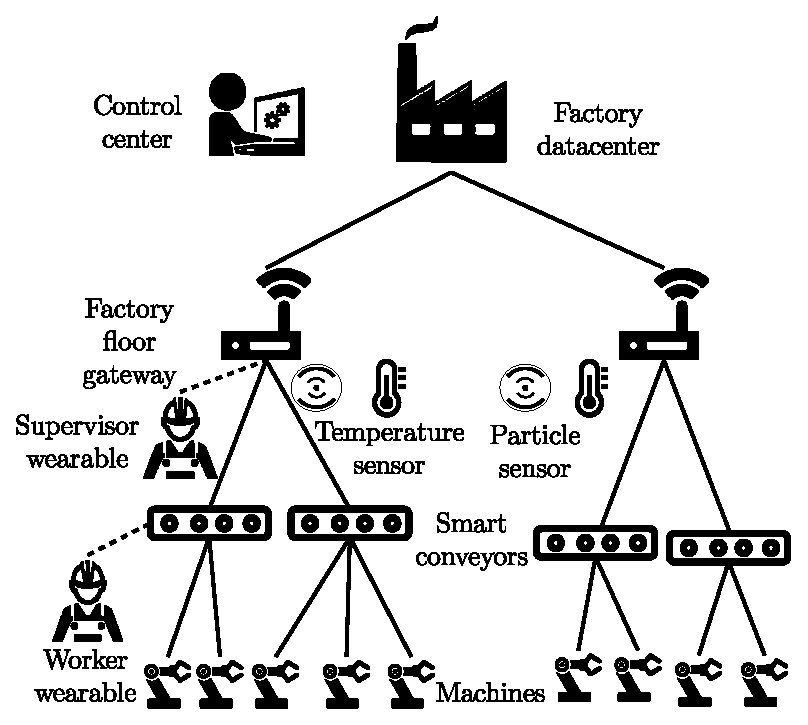
\includegraphics[width=\textwidth]{figures/use_case2.eps}
	}
	\caption{Fog-enabled smart factory}
	\label{fig:usecase}
\end{figure}

Let us consider a production plant divided into two floors, processing different kinds of products. 
These floors are modular: the plant structure is subject to change in order to adapt to new productions.
Each floor is equipped with conveyor belts carrying products from machine to machine for transformation. 
Devices are organized hierarchically: machines are connected to conveyors that are connected to the floor gateway that itself collects and delivers data to the factory datacenter. 
The factory is equipped with sensors in order to ensure the safety of workers: each floor is equipped with presence, luminosity, particle and temperature sensors, and the workers are equipped with wearables communicating with nearby conveyors.
Observations from the different sensors are used in order to identify potentially harmful situations, and then notify the control center, where actions can be taken remotely.
Unsafe situations are described with deduction rules, based on the semantic description of observations and of the environment.
For instance, 
%``the activation of a machine creating sparks in an atmosphere loaded with particles creates a detonation hazard'' is a potential rule.
``The presence of a worker near an operating conveyor in a low luminosity environment is a personal security hazard'' is a potential rule.
Some rules are also dedicated to quality insurance: sensors available in the factory, such as temperature sensors, or sensors integrated to machines and to the conveyor, enable the continuous control of production quality.
Some operations are temperature-sensitive, and a quality insurance rule is ``The detection of a temperature above a certain threshold while machines are operating is a break in the cold chain''.
As safety and quality insurance are time-sensitive applications, rule processing should be as fast as possible.
Moreover, the mobility of some sensors (\textit{e.g.,} worker wearables), combined with the modularity of the factory floors, create a dynamic network topology that evolves over time.

\subsection{Scalability}

Due to the modularity of the factory, the number of devices in the environment is not bounded a priori. 
In the specific industry 4.0 use case, this device count is unlikely to increase by multiple orders of magnitude, contrary to application domains of the \gls{iot} such as smart cities or connected vehicles, where large volumes of devices are involved.

Therefore, \textbf{scalability} is an important characteristic for a \gls{swot} system, and the decentralization of reasoning is an enabler of such scalability \cite{Maarala2017}.
However, the difference of computing power between Cloud and Fog nodes should not be neglected: the intrinsic capabilities of Cloud architectures enable a resource upscale impossible for Fog architectures.
Moreover, Cloud infrastructures provide a stability that is complementary to the dynamic nature of Fog architectures.
We propose therefore to leverage both the distributed nature of Fog computing and the permanent, powerful nature of Cloud computing by adopting a mixed approach. 

\subsection{Responsivity}

In the proposed use case, the rules deployed in the system are used to detect potentially harmful situations, requiring the inferred notifications to be received by the control center as soon as possible. 
The proposed system should be able to reduce as much as possible the time from the appearance of an undesirable situation, and the moment where the control center is notified of such situation.
\textbf{Responsivity} therefore is another desirable characteristic for our contribution.

Fog-enabled architectures trade computational power for proximity with data sources, which reduces the number of hops between data production and data processing. 
This reduces delays due to message delivery to distant Cloud nodes, and it is also interesting for situations where increasing the proximity with data sources decreases the complexity of reasoning.
When decentralizing processing, the individual computational load is reduced for each node compared to a centralized approach, which can yield better performances \cite{Su2018}.
Instead of funneling all the data towards the Cloud before inferring higher level information, combining Fog computing and direct communication between Fog nodes and applications should enable a faster notification delivery.

%\Nicolas{Voir commentaire pour détailler la généricité de l'approche}
%\subsection{Applicative logic modularization requirement}
%
%Since our aim is to distribute rule among several nodes, \textbf{strategies must be developed in order to deploy computation on nodes}. 
%Each node has intrinsic characteristics allowing them to process or not given rules successfully. 
%We thus propose to base the strategies on node ad-hoc criteria depending on application requirements. 
%Such characteristics will drive the placement of rules among nodes.
%
%It is important to emphasize that deployment strategies are application-specific, since they are driven by application-level requirements.
%
%Similarly to an abstract class in an object-oriented paradigm, \gls{edr} should define \textbf{generic functionalities} to support distributed reasoning, and must be instantiated with a deployment strategy to build a concrete approach.

\subsection{Dynamicity}

\gls{iot} systems are dynamic by nature: they are open systems, where devices can appear and disappear, as well as move from one point to the other. 
In the smart factory use case we introduced, the modularity of the factory floors might lead to changes in the network.
More frequently, failures might happen, disconnecting a device. 
For energy saving purposes, not all the machines might also be powered permanently.
Moreover, some devices are attached to workers that are mobile: they will be connected to different machines over time, leading to a dynamic network topology.

As the placement of rules in the network should adapt to the evolution of the topology, the last characteristic that we want for \gls{edr} is \textbf{dynamicity}.
Depending on the devices available at a given moment on a given node of the network, not all the applicative rules will necessarily be relevant to this node.
If a rule requires observations from a sensor that disconnects, carrying on applying this rule is a waste of resources. 
Applications consuming \gls{iot} data are also subject to change, and adapting the rule distribution strategy depending on the applications is also an aspect of dynamicity we consider.
%\Nicolas{voir commentaires pour plus de détails qui me paraissent redondants avec l'overview EDR}

%The criteria for this relevance is specific to the application that submitted the rule, and to the the distribution strategy this application aims to implement.
%Therefore, focusing on a single deployment strategy only supports the deployment of applications sharing the same requirements.
%The purpose of our contribution is to foster multiple application types, and therefore to support different deployment strategies.
%A requirement for \gls{edr} is thus to be \textbf{agnostic to the deployment strategy}.
%Since rules are elements necessarily dependent on applicative logic, we propose to embed the application-dependent deployment strategy within the rules.
%Each node handling a rule will thus be able to propagate it towards other Fog nodes according to this embedded deployment strategy.

%The strategy considering characteristics of nodes in the deployment process, such characteristics should also be propagated among the nodes, in order for a given node to decide if the rule needs to be deployed.
%To this end, some node functionalities are designed to support information propagation among nodes, enforcing the decentralized nature of the \gls{edr} approach.
%Another requirement for \gls{edr} is that \textbf{each node should only depend on information that is available locally} when executing the deployment strategy.
%If a central controller was involved when a rule is propagated, then the burden of central computation would be shifted to a burden of centralized topology awareness, where a unique node would have a global perception of the topology.
%Such an oracle would be able to efficiently place rules according to the deployment strategy, but such an approach is not scalable.
%The dynamism of the topology would require a constant communication directed to a single point, and the oracle would need to have a complete representation of the topology, which could represent a large number of nodes. 
%
%The locality of decision-making requires nodes to exchange information continually to maintain a representation of their environment consistent with the evolving reality.
%The two characteristics we identified, the embedding of the propagation strategy into rules and the continuous exchange of information among nodes, are two complementary elements enabling a third desirable property for \gls{edr}: its \textbf{dynamicity}.
%\gls{edr} is meant to support deployment in Fog environment, in which resources are partially constrained. 
%To limit resource consumption, \textbf{\gls{edr} should adopt an event-driven behavior}, in which messages are pushed from one node to another when an event occurs.
%Such behavior is opposed to poll-based or time-driven behaviors, where messages are exchanged constantly with no guarantee that a relevant information is conveyed.
%The event-driven nature of \gls{edr} enables the continuous adaptation of the rule deployment to the state of the topology. \newline

%The core of the \gls{edr} approach, implementing the characteristics identified in this section, is detailed in Section \textsection \ref{sec:edr}.
%Related work are studied in the next section \textsection \ref{sec:related_work_distribution}, in order to compare the characteristics we want for \gls{edr} to the state of the art.

\section{Related work for rule deployment in SWoT architectures}
\label{sec:related_work_distribution}

As the proposed approach sets out to deploy reasoning rules among Fog nodes to enable deducing application-dedicated information from \gls{iot} data, state-of-the-art work dealing with logical rules for the \gls{iot}, distributed reasoning and processing on constrained nodes is presented.

\subsection{Rules for the SWoT}
\label{subs:rules}

Rules are logical twofold elements, composed of preconditions and postconditions.
Preconditions represent a state of the world such that the rule should be applied in order to generate its post conditions, which represent a new state of the world.
In our literature search, we identified two main types of rules associated to the \gls{swot} \cite{Boley2007}:
\begin{itemize}
	\item \textbf{Production rules}, or deduction rules, in which preconditions are expressed as a logical expression, and postconditions are new knowledge which is the logical consequence of the preconditions.
	\item \textbf{\gls{eca} rules}, in which preconditions are the association of a logical expression and an event triggering its evaluation, and the postconditions are actions to be executed if the preconditions are matched. 
	Such actions are not limited to knowledge inference: they can be instantiated by running a piece of code.
\end{itemize}

As production rules are explicit deduction representations, they have been considered in \gls{iot} networks to express and share the correlation between sensor observations and high-level symptoms since early work on the \gls{swot} \cite{AmitSheth30}.
\cite{Sezer2018} lists numerous works using rules for context-awareness in the \gls{iot}.

With the goal of facilitating rule reuse, Linked Rules principles have been proposed \cite{Khandelwal2011}. 
They apply the basic principles of Linked Open Data and Linked Open Vocabularies to rules: rules are designated by dereferencable \gls{iri}s, expressed in W3C-compliant standards, and they can be linked to each other.
Inspired from the Linked Rules, the Sensor-based Linked Open Rules (S-LOR) \cite{Gyrard2017} is dedicated to rule re-usability for deductions based on sensor observations.
Production rules are a mechanism similar to \gls{cep} approaches, used for instance in \cite{ZangLi55}, but the rule representation shifts from an ad-hoc rule format in \gls{cep} to a unified format in the \gls{swot}. 

\cite{Sun2014} proposes a classification of production rules for the \gls{iot}, in order to identify recurring patterns.
The authors distinguish rules enabling deductions from relations between nodes, and from relations between events (\textit{i.e.} changes of the environment).
In our contribution, we go further than this distinction by manipulating hybrid rules: their preconditions may rely both on conditions expressed on the nodes of the network, or on their environment.

\subsection{Centralizing rule processing on Cloud nodes}

In most existing approaches, \textit{i.e.} \cite{ZangLi55}, \cite{Gyrard2017} or \cite{xu2017network}, production rules are handled by Cloud nodes.
An example of \gls{iiot} use case enabled by Cloud-based semantic rules processing is presented in \cite{Wang2018}.
This paper proposes a self-configuring smart factory: conveyors and machines produce data which is processed on a Cloud node where user rules are used to make reconfiguration decisions.
Rules are expressed in SWRL.
The same formalism is used in \cite{Rodriguez2010}, where production rules are computed in a central Cloud node in order to dynamically reconfigure the communication network topology between devices and the Cloud node.
The inferred deductions are converted into network reconfiguration actions by ad-hoc agents.
A similar hybrid approach is used in \cite{Evchina2015}: rules are expressed as production rules, but their postconditions may include ad-hoc properties dedicated to the triggering of actions.

In \cite{Kasnesis2015}, a multi-agent blackboard approach is chosen to dynamically manage rules in a smart home. 
Observations are published to a central node, the Domotic Status Board (DSB), where they are checked against rules in order to trigger inferences and reactions: the rules considered combine properties of production rules and \gls{eca} rules.
Rules are expressed in the Jena formalism\footnote{\url{https://jena.apache.org/documentation/inference/\#rules}}, and an interface also allows users to control the system based on controlled grammar sentences.
In this system, rules may be injected or deactivated at runtime.
\gls{eca} rules are also used in a smart home use case in \cite{Mainetti2015}: the authors propose an autonomic-like approach, where collected data is used to trigger actions of the system based on rules.
A distinction is made between two types of actions stored in the \gls{kb}: high-level actions, which are policies chosen by the user, and low-level actions, which are the actual implementations of the former, built by domain experts to hide the complexity of the system to the end-user.
User preferences are expressed through a GUI, and converted from the GUI to \gls{kb} individuals. 
During this conversion, appropriate low-level actions are selected to implement user-generated policies.
The actual deployment topology is not presented, but the absence of any element indicating a distribution of the underlying platform leads to the conclusion that it is executed on a central node.

Production rules are used for context-awareness in a smart user space in \cite{Hussein2016}.
Location information is combined to business knowledge, and to observations of the state of the user's environment, in order to make assumptions on the context.
For instance, the following is a rule introduced by the authors: ``IF the user is in an airport lounge with a low luminosity and the drapes closed THEN the user is sleeping''.
Such deduction is then used by context-aware services to adapt their behavior, materialized by \gls{eca} rules.
Data required for the deductions are gathered into a central hub before being processed, and deductions are then sent to remote nodes.

%An observation that was made in the previous chapter \textsection \ref{chap:survey} regarding context scale is confirmed in the work that are described here. 
Rules are deported on Cloud nodes rather than executed in Fog nodes when used to achieve context-awareness, such as in \cite{Evchina2015} or \cite{Hussein2016}, in order to obtain a global execution context.
However, in \cite{Rodriguez2010} for instance, some reconfiguration decisions could be taken considering only a local context. 
In this case, rules could be executed directly on Fog nodes.

\subsection{Distributing rule processing on Fog nodes}

The centralized architecture of the previously described papers raises issues such as the cost of semantic reasoning that increases rapidly with the size of the \gls{kb} \cite{Maarala2017}.
Fog computing offers a low-latency, resilient alternative for rule processing, even though the constrained nature of Fog nodes (compared to Cloud nodes) must be taken into account: processing power or bandwidth are critical resources.
Centralization also requires all the content collected by \gls{iot} devices to be processed in the same place, while Fog computing makes computing power available closer to \gls{iot} devices.
Fog computing enables contentto be processed with rules \textbf{where it is produced}, rather than requiring it to be transported to a remote node to be processed by Cloud computing.
Rule placement in Fog architectures is thus a topic of interest for the \gls{swot}

Most approaches for processing on constrained nodes focus on optimizations enabling such processing for a single node without considering the others.
When considering a distributed execution composed of several Fog nodes, processing placement is not dynamic: all nodes execute the same rules, or each a predefined rule set statically assigned.
For instance, even though it is not directly targeted at \gls{swot} applications, the RETE algorithm proposed in \cite{Woensel2018} is dedicated to constrained nodes.
RETE aims at reducing the memory requirements for production rule processing.
This is a very interesting optimization, but it is dedicated to a single Fog node and does not consider distributed processing.
\cite{Desai2015} shows how gateways are Fog nodes capable of enriching data: observations are initially produced by legacy devices in ad-hoc formats. 
It is the gateway, communicating with devices using protocols adapted to constrained environments, such as CoAP, that enriches the data before forwarding it towards a Cloud node. 
Observations are therefore enriched on the edge of the network, and only the Fog nodes in direct contact with legacy devices have to perform data enrichment.
\cite{Lee2016} or \cite{KaedKBHS18} propose to execute \gls{eca} in Fog architectures, used to automate the response of the system to a stimulus. 
However, both authors only consider one gateway executing the rules, and the ad-hoc rule format is not suited for rule exchange.
The contribution introduced in \cite{IoannisChatzigiannakis129} uses \gls{eca} rules associated to \gls{sw} formalisms, namely SWRL and SPARQL.
The authors use the Wiselib RDF provider \cite{Hasemann2012}, as well as CoAP and 6LowPan communication, in order to enable semantic processing directly on constrained nodes.
How rules are distributed in the network is not discussed.

Regarding processing distribution in existing work, the dynamic nature of \gls{iot} networks should be considered. 
The topology of a network evolves as devices connect, disconnect, or move geographically.
Therefore, a viable distribution of rules at a given moment is not guaranteed to remain optimal in the future, and \textbf{the distribution strategy should be adapted to the evolution of the network topology}.
\cite{Maarala2017} does not detail the mobility strategy used for its mobile nodes, and each node applies all the rules regardless of their relevance to the content it aggregates.
In \cite{Su2018}, rule placement is static, in either Cloud or Fog nodes. 
\cite{Taneja2017} focuses on resource placement in a Fog-enabled \gls{iot}. 
The authors compute optimal deployment of application modules based on the representation of available resources in the Fog architecture compared to requirements expressed by applications. 
Module positions are static, and computed at the time of deployment.
Rules are deployed on gateways in an \gls{iiot} context in \cite{Kaed2018}.
The rules themselves are not expressed using \gls{sw} formalisms, but they are combined to a semantic engine proposed in \cite{Kaed2016} in order to consume enriched data.
The placement of rules in the Fog architecture is not dynamic, however ad-hoc mechanisms enable rule update at runtime.

\gls{edr} differs from previous proposals by several aspects in order to comply with the requirements described in Section \textsection \ref{sec:edr_characteristics}:
\begin{itemize}
	\item The locality of the knowledge involved in the rule deployment: each node only considers its own \gls{kb} when propagating a rule.
	\item The \textbf{dynamicity} of rule deployment in the \gls{swot} system at runtime, constantly adapting to the state of the topology in an event-driven behavior.
	\item The \textbf{genericity} of the approach, enabling its adaptation to various application-level strategies.
\end{itemize} 

\section[Distributing reasoning with EDR]{EDR, a generic approach to dynamically distributed rule-based reasoning}
\label{sec:edr}

In this section, \gls{edr}, a generic approach to dynamically distributed rule-based reasoning supported by semantic Fog computing, is introduced. 
\gls{edr} is based on architectural assumptions that are presented in Section \textsection \ref{subs:edr_asumptions}.
\gls{edr}'s functional overview is depicted in Section \textsection \ref{subs:edr_overview}, before presenting the vocabulary used to describe \gls{edr} core functionalities in Section \textsection \ref{subs:edr_vocabulary}.
Modular rules are at the core of \gls{edr}, the formalisms used to represent them and the roles of their modules is described in Section \textsection \ref{subs:edr_rules}.

\subsection{Assumptions on the underlying architecture}
\label{subs:edr_asumptions}

\gls{edr} is based on the hypothesis of a \textbf{hierarchical network topology}: nodes are organized in a tree-like structure, and only communicate with neighboring nodes, \textit{i.e.} Cloud node and semantic-computing-enabled Fog nodes. 
%End \gls{iot} devices are not considered as semantically-enabled in order to accommodate legacy devices, and they are seen  
The neighbours of a node are either its (unique) parent, or its children nodes. 
This assumption is made because such topologies are frequent in \gls{iot} networks, represented in studies such as \cite{Rodriguez2010}, \cite{Zanella2014}, \cite{Alaya2015} (based on the oneM2M standard), \cite{Szilagyi2016}, or \cite{Su2018}.
Based on this hypothesis, it can be assumed that there only is one path from any node to any of its ancestors, which simplifies our approach.

Applications are not deployed on a Cloud node belonging to the \gls{iot} topology: they are executed remotely on personal devices such as smartphones or laptops.
\textbf{Rules represent applicative needs}: when deductions from sensor observations are required by an application, it injects the rule in the network in order to be provided directly with the deductions, instead of being forwarded raw data by the network and applying the rules itself.

It is therefore assumed that \textbf{Fog nodes can communicate with applications directly}.
Rules are initially submitted by applications to the Cloud node, so it is the only node they know \textit{a priori}. 
The Cloud infrastructure provides a unique permanent interface to the network, the dynamic Fog topology underneath is therefore transparent for applications.

We qualified the \edr as "dynamic", because nodes constantly re-evaluate their past decisions (\textit{e.g} rule management or data propagation). 
Whenever an event occurs that may impact the current distribution of the rules in the network, each node locally recomputes the decision algorithm shown on Fig. \ref{fig:edr_algo}, and introduced in the remainder of this section.
However, the proposed approach will adapt to the evolutions of the underlying topology based on the assumption that all events impacting the topology are considered by the appropriate nodes.
In particular, the failure of a node must be captured by its parent, which must then propagate the consequences of this event on its own behavior to the rest of the network.
%Such failure management mechanism could be integrated to some existing standards, such as oneM2M, acting as a middleware.
Therefore, we consider failure management to be handled in the middleware layer, and it does not need to be explicitly handled in the scope of the applicative layer proposed in this contribution.

\subsection{Overview of the EDR approach}
\label{subs:edr_overview}

In order to ensure decentralization, the algorithm of the \gls{edr} approach is executed in parallel on each node able to perform reasoning in the topology. 
\gls{edr} considers a neighbor-to-neighbor rule and data propagation, enabling a reduction the nodes' knowledge of the topology to a limited subset of the complete deployment. 
Thus, consistency of the knowledge only has to be maintained with neighbors, which limits required knowledge-related exchanges between nodes, and improves scalability.
Due to the potential mobility and variable availability of Fog nodes, \textbf{\gls{edr} is meant to foster decision making in a local context for each node, leading at a large scale to the dynamic emergence of a desirable behavior}.

A parent node propagates a rule to its child if the parent considers that the child is empowered to apply the rule.
This decision is made by the parent based on a \textbf{deployment strategy} embedded in the rule, as well as on the knowledge it has of said child.
The deployment strategy captures the \textbf{criteria required for a node to process a rule}, and therefore characterizes if a child node is suitable to be forwarded said rule.
In order to enable rule deployment, nodes exchange messages describing their characteristics, \textit{e.g.,} their location, the type of data they observe, or the type of data they are interested in.
To ensure the \textbf{dynamicity} of the rule deployment with respect to the \textbf{evolving network topology}, these messages are exchanged constantly, whenever nodes characteristics are modified.
When a node makes a new deduction based on a rule, it sends the result to all the nodes it knows to be interested, including the application that submitted the rule.

\textbf{The \gls{edr} approach itself is agnostic to the deployment strategy}, which is defined by the rule implementer: that is why we qualify \gls{edr} as \textbf{generic}. 
The present section \textsection \ref{sec:edr} is dedicated to the \gls{edr} approach, which defines the characteristics of a deployment strategy without implementing them.
Such implementation is described with a refinement of \gls{edr}, \edrt, introduced in Section \textsection \ref{sec:edrpt}.

\begin{figure*}
	\centering
	\caption{EDR node-centric functional overview}
	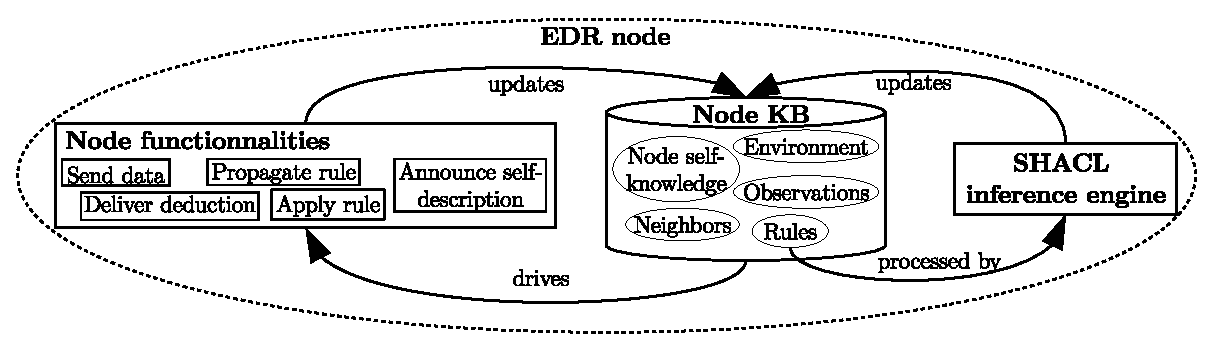
\includegraphics[width=0.85\textwidth]{figures/overview.eps}
	\label{fig:node_overview}
\end{figure*}

A functional representation of an \gls{edr} node is provided in Fig. \ref{fig:node_overview}: each node has a local \gls{kb}, where knowledge necessary to the execution of \gls{edr} is stored.
This knowledge is used to drive the basic functionalities of the node, and rules are used by the inference engine to update the \gls{kb}.

Featured knowledge includes:
\begin{itemize}
	\item the knowledge the node has of its own characteristics,
	\item the knowledge it has about its neighbors,
	\item the knowledge it has about the static organization of the environment such as the geographic or indoor location, or the relationship between the surrounding elements,
	\item the value of the last observations depicting the current state of the dynamic features of the environment,
	\item the rules that it has received from either applications or other nodes.
\end{itemize}

This knowledge is used to control the behavior of the node, composed of simple functionalities.
A node is able to:
\begin{itemize}
	\item Send a piece of data, typically a sensor observation, to a remote node,
	\item Propagate a rule to a remote node,
	\item Apply a rule on its knowledge base,
	\item Announce a description of its own characteristics to a remote node,
	\item Deliver a deduction obtained by processing a rule to a remote node, 
\end{itemize}

How these node functionalities are related to the \gls{kb} in the core \gls{edr} mechanism to enable the propagation of observations and rules is described in Section \textsection \ref{subs:edr_vocabulary}.
The modular rule representation embedding the deployment strategy, and the updates of the \gls{kb} they trigger, are detailed in Section \textsection \ref{subs:edr_rules}.
In this paper, the focus is on the propagation of rules, and on their execution, which leads to the production of new information. 
How this information may be used by the nodes to trigger real-world actions is not in the scope of this contribution. 
Using high-level deduction to trigger actions in an autonomic loop has been the topic of previous work \cite{Seydoux2016}.

\subsection{A vocabulary driving the deployment mechanism}
\label{subs:edr_vocabulary}

Node behavior is made quite simple on purpose, in order to decorrelate the rule-specific deployment strategy from the core algorithm on which \gls{edr} is based.
Rule deployment strategies are dedicated to a particular purpose, \textit{e.g.,} response time reduction or privacy enforcement, while \gls{edr} is generic.
%, and therefore agnostic to deployment strategies.
In order to support the genericity of \gls{edr} with a knowledge-driven method, node functionalities are based on a dedicated vocabulary, used to describe knowledge in the node's \gls{kb}.

For instance, this vocabulary captures the hierarchical nature of the topology.
Let the set of children of node $n$ be referred to as $Children(n)$, and the singleton containing $n$'s parent be noted $Parent(n)$.
The relation between a node $n$ and any $n_c\in Children(n)$ is expressed with the triple \triplet{$n$}{\concept{lmu}{has\-Downstream\-Node}}{$n_c$}\footnote{Namespaces are available in Appendix \ref{app:namespaces}}$^,$\footnote{Individuals such as $n$ and $n_c$ are identified with an \gls{iri} in the triples}, based on a nomenclature presented in \cite{Seydoux2017}. 
The inverse relation exists, to express the connection between a node $n$ and its parent $n_p\in Parent(n)$: \triplet{$n$}{\concept{lmu}{has\-Upstream\-Node}}{$n_p$}.

A description of all the functionalities of the nodes, and of the vocabulary that drives them, is provided in Section \textsection \ref{subsubs:basic_functionalities}. 
Further details about the announcement functionality are provided in Section \textsection \ref{subsubs:annouce}, especially with regard to the consumption of data.
Finally, the scope of the announcements is studied in Section \textsection \ref{subsubs:proxying}.

\subsubsection{Basic node functionalities}
\label{subsubs:basic_functionalities}

Each functionality relies on dedicated triples, and a node implements its behavior based on the description held in its \gls{kb}.
How these triples are inferred from the deployment strategy is described in the next section \textsection \ref{subs:edr_rules}.
Before detailing how the strategy triggers nodes functionalities, let us examine the vocabulary describing said node functionalities.

\paragraph{Announce self-description:}
When a node connects, disconnects or changes characteristics, it notifies its neighbors of its self-representation.
Since a notification is sent at each update of the node's state, the perception of a node by its neighbors remains consistent with its evolution over time.
Two mechanisms support this announcement: 
\begin{itemize}
	\item a partial update, in which a node adds statements to its description already held by the target
	\item a complete update, in which the representation of the node is completely erased by the target before being updated.
\end{itemize}
These mechanisms add information about a node by exchanging light messages containing partial representations, while removing outdated statements with the complete update. 
A particular node characteristic that is declared in the announcement functionality is the type of data in which a node is interested, captured with the predicate \concept{edrt}{is\-Interested\-In}, which is used in the data sending functionality.
The announcement functionality is extended by the mechanisms described in Section \textsection \ref{subsubs:annouce} to control which characteristics of the node are propagated, and the scope of this propagation in Section \textsection \ref{subsubs:proxying}.

\paragraph{Apply rules:}
When a node $n$ receives a new observation, either from its own sensors or children, $n$ executes the rules $r$ stored in its \gls{kb} if the description of $r$ contains \triplet{$r$}{\concept{edr}{is\-Rule\-Active}}{true}.

\paragraph{Deliver deduction:}
\label{par:deduction_delivery}
If the processing of an observation with rule $r$ by node $n$ leads to a deduction $\delta$, $\delta$ is sent to each node belonging to $\bigcup n_{consumer}$ where \triplet{$n_{consumer}$}{\concept{edr}{consumes\-Result}}{$r$} is in the \gls{kb} of $n$.
The application that submitted the rule $r$ to the network is known as the rule originator $o$, and is represented by the triple \triplet{$r$}{\concept{edr}{rule\-Originated\-From}}{$o$}.
The originator of a rule is considered as a consumer of rule results, in order to enable deduction delivery to applications.
The deduction delivery functionality is separated from the interest notification part of the announcement functionality for flexibility.

\paragraph{Send data:}
\label{par:data_transfer}
When node $n$ receives an observation of type $\rho_t$, if $n_p \in Parent(n)$ has declared its interest for this type, the observation is forwarded toward $n_{p}$.
Observations are exchanged lazily: if a node $n$ receives an observation of type $\rho_t$, and knows no other node interest in such type, the observation is not forwarded.
Such interest is represented in node $n$ \gls{kb} with the triple \triplet{$n_{p}$}{\concept{edr}{is\-Interested\-In}}{$\rho_t$}.
The notification of the interest is considered as a characteristic of the node, managed in the announcement functionality.

\paragraph{Propagate rule:}
\label{par:send_rule}
A node sends a rule to one of its neighbors if it considers that its target is capable of applying the rule, such a consideration being part of the rule deployment strategy. 
In the case where rule $r$ should be propagated towards node $n_{target}$ by $n$, the triple \triplet{$r$}{\concept{edr}{transferable\-To}}{$n_{target}$} is present in $n$'s \gls{kb}.

\subsubsection{Controlling node characteristics propagation}
\label{subsubs:annouce}

The \gls{edr} algorithm depends on the exchanges between neighboring nodes of their mutual descriptions, enabled by the announcement functionality.
However, presupposing node characteristics relevant to any deployment strategy that will be implemented to refine \gls{edr} is not possible.
In order to remain agnostic to the deployment strategy, \gls{edr} relies on a dedicated vocabulary used to describe which of each node's characteristics should be announced to its neighbors. 
A node has two types of neighbors: its parent, and its children, and since the parent is unique (according to our assumptions) while the children are potentially many, two approaches are devised.

\paragraph{Announcing characteristics to a node's parent:}
Let us consider a node $n$, with a characteristic represented by a property $has\-Charac\-teris\-tic$ and captured in its knowledge base such that \triplet{$n$}{$has\-Charac\-teris\-tic$}{$\nu$}, with $\nu$ either a literal or an individual.
When announcing its characteristics to its parent, $n$ searches in its \gls{kb} for all the triples where it is the subject, and the predicate is typed as \concept{edr}{Parent\-Announced\-Property}.
If the property $has\-Charac\-teris\-tic$ is such that \triplet{$has\-Charac\-teris\-tic$}{\concept{rdf}{type}}{\concept{edr}{Parent\-Announced\-Property}}, then the triple \triplet{$n$}{$has\-Charac\-teris\-tic$}{$\nu$} is part of the self description sent by the node $n$ to its parent because $has\-Charac\-teris\-tic$ is considered a relevant characteristic of $n$.

\paragraph{Announcing characteristics to a node's children:}
The announcement mechanism from parent to children is quite similar to the one from children to parent, with the difference that children may be many.
Therefore, the class \concept{edr}{Children\-Announced\-Property} has two subclasses to distinguish two possible cases:
\begin{itemize}
	\item \concept{edr}{All\-Children\-Announced\-Property} denotes a characteristic that is systematically announced to all the node's children.
	\item \concept{edr}{Some\-Children\-Announced\-Property} denotes a characteristic that should only be announced to a subset of the node's children. 
\end{itemize}
This distinction is made to give flexibility to the deployment strategy designers.

In the case of a characteristic captured by a predicate of type \concept{edr}{Some\-Children\-Announced\-Property}, each child eligible to be proxied the new characteristic must be represented explicitly with the predicate \concept{edr}{announce\-To}, which requires the reification of the announced characteristic.
In order to be announced towards child node $n_{c}\in Children(n)$, the triple \triplet{$n$}{$has\-Charac$}{$\nu$} is transformed into the following reified statement: 
$statement$ $rdf$:$subject$ $n_{c};$ $rdf$:$predicate$ $has\-Charac;$ $rdf$:$object$ $\nu;$ $edr$:$an\-nounce\-To$ $n_{c}$. 
The choice of the children to which the characteristic should be announced is application-specific, and is therefore part of the deployment strategy.
As the rest of the deployment strategy, it is embedded in rules as described in Section \textsection \ref{subs:edr_rules}.

The interest of a node for a type of data, denoted by the predicate \concept{edr}{is\-Interested\-In}, is managed as a node characteristic.
Therefore, depending on the deployment strategy, the interest of nodes is classified as one of the subclasses of \concept{edr}{Children\-Announced\-Property}.
More details about this particular predicate are provided in Section \textsection \ref{sec:edrpt}, with the instantiation of a concrete deployment strategy.

\subsubsection{Propagating knowledge beyond neighbors}
\label{subsubs:proxying}

\gls{edr} is designed for neighbor-to-neighbor rule and data propagation: a node $n$ only communicates with $n'\in Parent(n)\cup Children(n)$ (with the exception of deduction delivery).
However, such design may hamper the propagation of rules, by preventing the diffusion of knowledge required by the deployment strategy to make decisions as to where the rules should be placed.
We want to avoid the situation in which the characteristics of a node $n_{c}\in Children(n)$ makes it adequate to apply a rule which is held by $n_{p}\in Parent(n)$, but $n$ cannot apply the rule, and therefore $n_{p}$ does not propagate the rule to $n$, preventing its eventual propagation to $n_{c}$.
A complementary functionality is thus described by the \gls{edr} vocabulary to enable such diffusion of knowledge describing node characteristics: \textbf{proxying}.

The proxying mechanism implemented in \gls{edr} is inspired from \cite{Nikoli2011}, where reasoning nodes act as proxy for the characteristics of legacy nodes unable to process enriched data. 
In \gls{edr}, each reasoning-enabled node has a similar role, and proxy characteristics of its neighbors. 
Such proxying is bidirectional: the characteristics of a node's parent are proxied towards its children, and vice versa.
Specifically, node $n$ proxying a characteristics of $n_{p}\in Parent(n)$ towards any $n_{c}\in Children(n)$ means that $n$ announces such characteristics to $n_{c}$ as if it were its own.
An example of proxied node characteristics, detailed in Section \textsection \ref{subsub:topology}, is the interest of a node for a data type, briefly introduced here for the sake of illustration.

If a node $n$ wants to be notified whenever a temperature observation is available, it notifies its children $n_{c}\in Children(n)$ of such interest. 
If any $n_{c}$ collects temperature observations, it will forward such observations towards $n$. 
Moreover, each $n_{c}$ will in turn notify that it is \textbf{itself} interested in temperature observations to any node $n_{cc}\in Children(n_c)$.
Any node $n_{cc}$ collecting a temperature observation will therefore send it to $n_{c}$, which will itself send such an observation to $n$.
The characteristic of the initial node $n$ (here, the interest in temperature) has indeed been proxied to $n_{cc}$ by $n_{c}$: $n_{cc}$ only has knowledge of $n_{c}$, and communication is kept strictly between direct neighbors.
To support this mechanism, two classes of properties are defined in the \gls{edr} vocabulary: \concept{edr}{Parent\-Proxied\-Property}, and \concept{edr}{Children\-Proxied\-Property}.

\paragraph{Characteristics proxied from children to parent:}
Let us assume that $n_{c}\in Children(n)$, and that $n_{c}$ has a characteristic expressed by the triple \triplet{$n_{c}$}{$has\-Cha\-racteri\-stic$}{$\nu$}, that should be proxied towards $n_{p}\in Parent(n)$.
Such information about the predicate $\nu$ is materialized by the triple \triplet{$has\-Characteri\-stic$}{\concept{rdf}{type}}{\concept{edr}{Parent\-Proxied\-Property}}.
When receiving the description of $n_{c}$, $n$ checks for the presence of properties classified as \concept{edr}{Parent\-Proxied\-Property}. 
Since $has\-Characteristic$ is such a property, the node $n$ updates its own representation towards $n_p$ by sending the triple \triplet{$n$}{$has\-Characteri\-stic$}{$\nu$}, therefore proxying the capacity of $n_{c}$.

\paragraph{Characteristics proxied from parent to children:}
The proxying mechanism from parent to children is similar to the one from children to parent.
Contrary to the announcement functionality, the multiplicity of children is not considered: all the children are proxied any received parent characteristic.
Such policy is made necessary by the locality of decision-making enforced by \gls{edr}. 
On the one hand, a node $n$ receiving a characteristic to proxy $n_{p}\in Parent(n)$ does not have the contextual knowledge that leads $n_{p}$ to announce this particular characteristic to $n$.
On the other hand, the node $n_{p}$ does not have a detailed knowledge of the topology below $n$, and therefore cannot make any assumptions about to which children in particular $n$ should proxy the characteristic of $n_{p}$.

It is possible that the proxying mechanism and the announcement mechanism lead to conflicting behaviors.
In particular, a node may have chosen not to announce a characteristic of its own to some of its children, but be required to proxy the same characteristic instead of one of its ancestors.
In this case, the proxying mechanism supersedes the announcement mechanism, and any proxied characteristic is processed as a \concept{edr}{All\-Children\-Announced\-Property}.
For instance, if a node $n$ did not announce its interest for a data type $\rho_t$ to $n_{c}\in Children(n)$, $n$ will nonetheless announce such interest to $n_{c}$ if $n_{p}\in Parent(n)$ notifies $n$ of its own interest for $\rho_t$.

\subsection{Rule representation and deployment}
\label{subs:edr_rules}

\subsubsection{Rule modular structure}

\gls{edr} rules are composed of several modules, as represented on Fig. \ref{fig:rule_modules}. 
Each of these modules enables some node functionalities:

\begin{itemize}
	\item The Rule propagation module triggers the rule forwarding functionality
	\item The Result delivery module triggers the result delivery functionality
	\item The Activation module triggers the rule application, the data consumption and the result delivery functionalities.
	\item The Rule core module contains the actual business logic of the rule
\end{itemize}

The intelligence regarding rule deployment is located in the rules, and not hard-coded into \gls{edr} or statically attached to nodes. 
The behavior of the algorithm at a global scale can thus be parameterized at a fine granularity, for each rule.
Rules are represented in SHACL, and the modules are based on the SHACL advanced functionality named ``SHACL rules''.
Each module is composed of two parts: a SHACL rule, that inserts deductions into the \gls{kb}, and a SHACL shape that determines whether the rule is applied or not. 
An example rule, named $r1$, is provided online \footnote{\url{https://w3id.org/laas-iot/edr/iiot/r1.ttl}}.
In the remainder of this section, a generic description of these rule modules and their roles is given, each illustrated in $r1$. 
An implementation is proposed in Section \textsection \ref{sec:edrpt}, where specific behaviors dedicated to a particular strategy are described.

\begin{figure}
	\centering
	\caption{Rule modules}
	\label{fig:rule_modules}
	\scalebox{0.68}{
		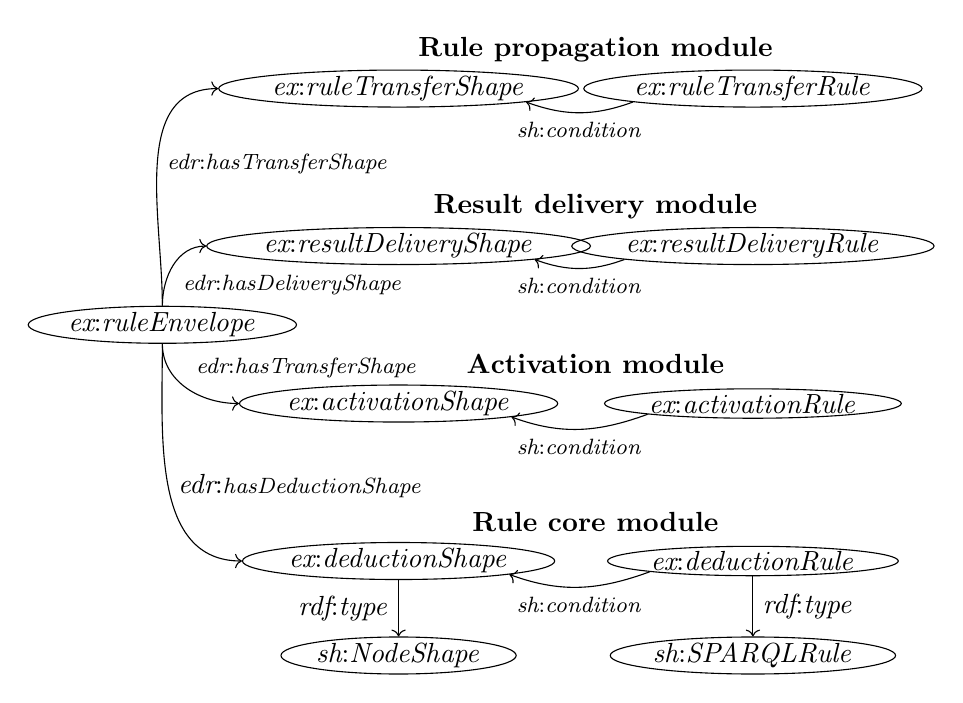
\begin{tikzpicture}
	\tikzstyle{concept}=[draw, ellipse, inner sep=0.01cm, shape aspect=0.5]
	
	\draw (0.5,0) node[concept] (envelope) {\concept{ex}{rule\-Envelope}};
	\draw (3.5, 3) node[concept] (transfershape) {\concept{ex}{ruleTransferShape}};
	\draw (3.5, 1) node[concept] (deliveryshape) {\concept{ex}{resultDeliveryShape}};
	\draw (3.5, -1) node[concept] (activationshape) {\concept{ex}{activationShape}};
	\draw (3.5, -3) node[concept] (deductionshape) {\concept{ex}{deductionShape}};
	
	\draw (8, 3) node[concept] (transferrule) {\concept{ex}{ruleTransferRule}};
	\draw (8, 1) node[concept] (deliveryrule) {\concept{ex}{resultDeliveryRule}};
	\draw (8, -1) node[concept] (activationrule) {\concept{ex}{activationRule}};
	\draw (8, -3) node[concept] (deductionrule) {\concept{ex}{deductionRule}};
	
	\draw[->] (envelope.north) to[out=90, in=180] node[right] {\footnotesize \concept{edr}{hasTransferShape}} (transfershape);
	\draw[->] (envelope.north) to[out=90, in=180] node[below right] {\footnotesize \concept{edr}{hasDeliveryShape}} (deliveryshape);
	\draw[->] (envelope.south) to[out=270, in=180] node[above right] {\footnotesize \concept{edr}{hasTransferShape}} (activationshape);
	\draw[->] (envelope.south) to[out=270, in=180] node[right] {\concept{edr}{\footnotesize hasDeductionShape}} (deductionshape);
	
	\draw[<-] (transfershape.south east) to[out=340, in=200] node[below] {\footnotesize \concept{sh}{condition}} (transferrule.south west);
	\draw[<-] (deliveryshape.south east) to[out=340, in=200] node[below] {\footnotesize \concept{sh}{condition}} (deliveryrule.south west);
	\draw[<-] (activationshape.south east) to[out=340, in=200] node[below] {\footnotesize \concept{sh}{condition}} (activationrule.south west);
	\draw[<-] (deductionshape.south east) to[out=340, in=200] node[below] {\footnotesize \concept{sh}{condition}} (deductionrule.south west);
	
	\draw (6, 3.5) node {\textbf{Rule propagation module}};
	\draw (6, 1.5) node {\textbf{Result delivery module}};
	\draw (6, -0.5) node {\textbf{Activation module}};
	\draw (6, -2.5) node {\textbf{Rule core module}};
	
	\draw (3.5, -4.2) node[concept] (nodeshape){\concept{sh}{NodeShape}};
	\draw (8, -4.2) node[concept] (sparqlrule) {\concept{sh}{SPARQLRule}};
	\draw[->] (deductionshape) -- node[left] {\concept{rdf}{type}} (nodeshape);
	\draw[->] (deductionrule) -- node[right] {\concept{rdf}{type}} (sparqlrule);
\end{tikzpicture}
	}
\end{figure}

In order to associate all the modules to a rule represented as a single individual in a node's \gls{kb}, we introduce the notion of \textbf{rule envelope} as a reification mechanism. 
The envelope of an \gls{edr} rule is an individual subject of triples whose predicates are \concept{edr}{has\-Transfer\-Shape}, \concept{edr}{has\-Apply\-Shape}, \concept{edr}{has\-Delivery\-Shape} and \concept{edr}{has\-Deduction\-Shape}.
The rule envelope is especially useful in the rule deployment process, when all the modules of a given rule must be collected for the rule to be propagated to a remote node.
%The envelope of a rule $r$ is denoted $r^{envelope}$.

\subsubsection{Rule modules}
\label{subsubs:modules}

\paragraph{Core module}
The operational part of the rule, containing the application-dedicated inference, is referred to as the \textbf{rule core} module. 
The core module is based on a predicate logic rule used to deduce high-level information, similar to the rules introduced in the use case in Section \textsection \ref{sec:distribution_use_case}. 
Let $r^{core}$ be such a rule core module, noted as $r^{core}: \Gamma_1 \land ... \land \Gamma_n \rightarrow \Delta_1 \land ... \land \Delta_m$, where $\Gamma_1 \land ... \land \Gamma_n$, designated as the \textbf{body} of $r^{core}$, is a conjunction of conditions and $\Delta_1 \land ... \land \Delta_m$, designated as the \textbf{head} of $r^{core}$, is a conjunction of deductions.
The rule core module only encompasses applicative deduction logic: it is unrelated to the deployment of the rule.
$r^{core}$ is only evaluated when the whole rule $r$ has been declared active on a node in the deployment process, \textit{i.e.} if the triple \triplet{$r$}{edr:is\-Rule\-Active}{true} is in the node's \gls{kb}.

\paragraph{Rule transfer module}
The \textbf{rule transfer module} determines on which remote nodes the rule may be deployed, according to a rule-specific deployment strategy.
This condition is expressed as a SPARQL query embedded in the SHACL rule being the conditional part of the rule transfer module.
The deduction part of the module infers the triple \triplet{$r$}{\concept{edr}{transferable\-To}}{$n'$}, enabling the rule forwarding mechanism of the node (\textit{c.f.} Section \textsection \ref{par:send_rule}).
The transfer module of a rule $r$ is denoted $r^{transfer}$.
%An extract of the SHACL rule of the transfer module for rule $r_{comfort}$, denoted $r_{comfort}^{transfer}$, is provided in Lst. \ref{lst:transferRule}.

%\begin{lstlisting}[float, caption=$r_{comfort}^{transfer}$ rule, label=lst:transferRule]
%CONSTRUCT {
%	ex:officeLightComfortRule edr:transferableTo $this.
%	ex:officeLightComfortRule edr:transferredFrom ?host.
%} WHERE {
%	$this lmu:hasUpstreamNode ?host.
%	?host a lmu:HostNode.
%}
%\end{lstlisting}

\paragraph{Rule activation module}
The \textbf{activation module} detects if the current node is suitable to apply the rule itself. 
If the conditional part of rule $r$ activation module determines that the current node is suitable to apply $r$, the activation of rule $r$ is made explicit by the triple \triplet{$r$}{\concept{edr}{is\-Rule\-Active}}{true}.
In the case where some node characteristics are conditionally proxied towards children (\concept{edr}{Some\-Children\-Proxied\-Property}), the rule activation module may infer reified statements as described in Section \textsection \ref{subsubs:proxying}. 
This case is illustrated in more detail in Section \textsection \ref{subs:edrt_modules}.
The activation module of a rule $r$ is denoted $r^{activation}$.

\paragraph{Result delivery module}
The \textbf{result transfer module} enables the forwarding of deductions to other nodes that are not the originator of the rule, such as the parent $n'$ of a node $n$ if $n'$ applies a rule $r'$ that consumes the deductions made by a rule $r$ applied by $n$.
By default, the originator $o$ of a rule $r$ is assumed to be interested in the results of $r$, denoted with \triplet{$o$}{\concept{edr}{consumes\-Result}}{$r$}.
If a remote node $n'$ is interested in the deductions made by rule $r$, the result transfer module infers that \triplet{$n'$}{\concept{edr}{consumes\-Result}}{$r$}.
%The result delivery module of a rule $r$ is denoted $r^{delivery}$.

%\begin{figure}
%	\centering
%	\caption{Relation between node functions and rules modules}
%	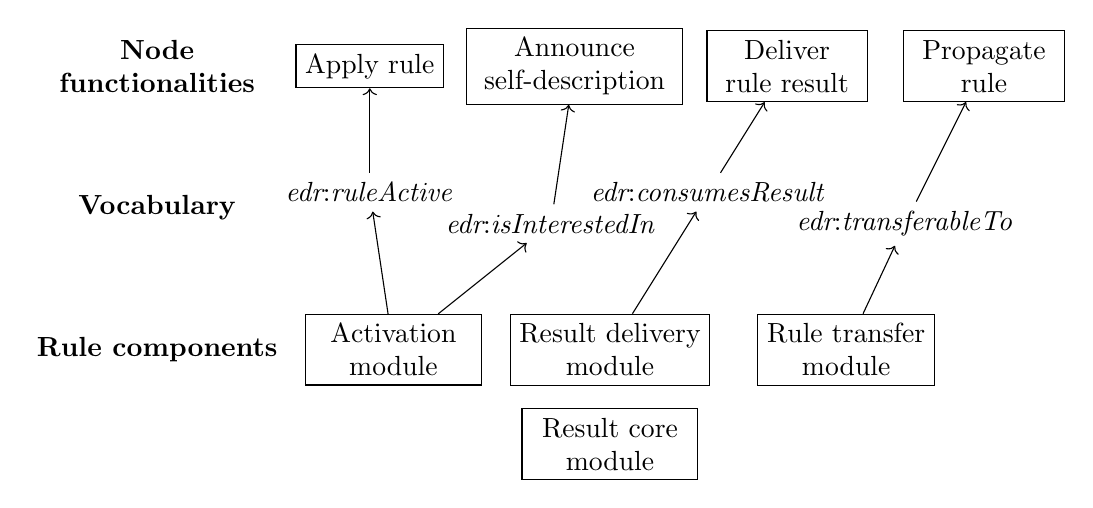
\begin{tikzpicture}
	\draw (0,0) node {\textbf{Rule components}};
	\draw (0,1.8) node {\textbf{Vocabulary}};
	\draw (-0,3.6) node {\pbox{2.5cm}{\Centering \textbf{Node}\\\textbf{functionalities}}};
	
	\draw (3, 0) node[draw, rectangle] (activation) {\pbox{2cm}{\Centering Activation module}}; 
	\draw (5.75, 0) node[draw, rectangle] (delivery) {\pbox{3cm}{\Centering Result delivery\\module}};
	\draw (8.75, 0) node[draw, rectangle] (transfer) {\pbox{3.5cm}{\Centering Rule transfer\\module}};
	\draw (5.75, -1.2) node[draw, rectangle] (core) {\pbox{2cm}{\Centering Result core module}};
	
	\draw (2.70, 2) node (active) {\concept{edr}{rule\-Active}}; 
	\draw (5, 1.6) node (interested) {\concept{edr}{is\-Interested\-In}};
	\draw (7, 2) node (consumes) {\concept{edr}{consumes\-Result}};
	\draw (9.5, 1.6) node (transferable) {\concept{edr}{transferable\-To}};
	
	\draw[->] (activation) -- (active);
	\draw[->] (activation) -- (interested);
	\draw[->] (delivery) -- (consumes);
	\draw[->] (transfer) -- (transferable);
	
	\draw (2.70, 3.6) node[draw, rectangle] (apply) {\pbox{2cm}{\Centering Apply rule}};
	\draw (5.3, 3.6) node[draw, rectangle] (announce) {\pbox{2.5cm}{\Centering Announce self-description}};
	\draw (8, 3.6) node[draw, rectangle] (deliver) {\pbox{1.8cm}{\Centering Deliver rule result}};
	\draw (10.5, 3.6) node[draw, rectangle] (propagate) {\pbox{1.8cm}{\Centering Propagate rule}};
	
	\draw[->] (active) -- (apply);
	\draw[->] (interested) -- (announce);
	\draw[->] (consumes) -- (deliver);
	\draw[->] (transferable) -- (propagate);
\end{tikzpicture}
%	\label{fig:node_rule}
%\end{figure}

%The relationship between node functionalities (represented in Fig. \ref{fig:node_overview}), the \gls{edr} vocabulary and the rule modules is shown in Fig. \ref{fig:node_rule}. 

\subsubsection{Dynamically managing modules activation}

The rule core must be computed each time a new observation is received by the node, in order to check if new deductions may be inferred.
However, it is worth noting that the other rule modules only need to be evaluated when the rule is received, or when the topology evolves, \textit{e.g.,} with new productions by children, new consumptions by parent, or nodes connecting/disconnecting.

The SHACL standard is such that by default, when reasoning on a \gls{kb} containing SHACL shapes and rules, all of them are considered\footnote{See Section \textsection 4.3 of the recommendation \url{https://www.w3.org/TR/shacl/\#validation-definition}}.
In order to reduce the computation load, and to only process rule modules when needed, a SHACL functionality is used: the reasoner does not consider shapes or rules $r$ such that \triplet{$r$}{sh:deactivated}{true}.
The modules of a rule $r$ are therefore only activated for a reasoning step when $r$ is received, or when the topology evolves.

The appropriate modules, \textit{i.e.} all except the core module, are classified as \concept{edr}{Node\-Sensitive\-Component} (as opposed to what would be a ``Content sensitive component'').
Therefore, a unique query activates or deactivates rule modules related to deployment, for all the rules stored in a node's \gls{kb}.

Deployment module management is represented on Fig. \ref{fig:edr_algo}, in an overview of the algorithm.
When a rule is initially received, all of its modules are active. 
No activation is required when receiving a new rule, marker (1) on Fig. \ref{fig:edr_algo}. 
The rule deployment update, marker (3) on Fig. \ref{fig:edr_algo}, is performed by the reasoner.
Since no other rule deployment module has been activated since the new rule has been received, and by default these modules are deactivated, only the deployment of the newly received rule is computed.

In the case where the node receives information about a topology update, such as the connection or disconnection of a node or the change of characteristics of a known node, it is possible that the rule deployment should be updated accordingly.
For this reason, for all the rules stored in the node's \gls{kb}, the deployment modules are activated upon the reception of a topology update, as seen in marker (2) on Fig. \ref{fig:edr_algo}.
The received change is then integrated in the \gls{kb}, and if necessary the new topology is propagated to parent nodes, before performing a reasoning step computing the deployment rule modules.
If the placement rule needs to be updated due to the topology change, the new deployment is enforced by activating or propagating rules in compliance with the deductions and the \gls{edr} vocabulary, before deactivating the rule deployment modules, marker (4) on Fig. \ref{fig:edr_algo}.

If the received message is an observation, no rule deployment update is required. 
The only active rule modules are the core modules for rules that the node should process, and they are used by the reasoner to test if new inferences are possible.
The marking and propagation of deductions is discussed in Section \textsection \ref{subsubs:unique_identification}.

\begin{figure}
	\centering
	\caption{\gls{edr} algorithmic overview}
	\label{fig:edr_algo}
	\scalebox{0.7}{
		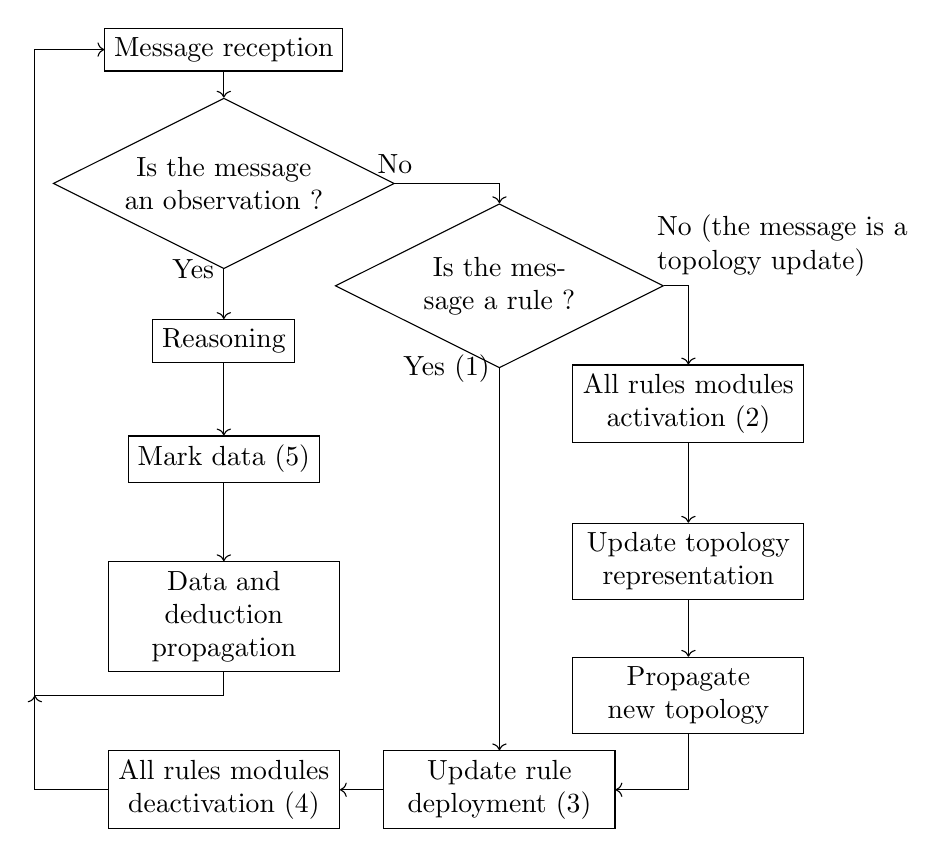
\begin{tikzpicture}
	\draw (-1,-0.3) node[rectangle, draw] (mess_reception) {Message reception};
	\draw (-1,-2) node[diamond, draw, aspect=2.0, inner sep=0] (test_obs) {\pbox{3.0cm}{\Centering Is the message an observation ?}};
	\draw (2.5,-3.3) node[diamond, draw, aspect=2.0, inner sep=0] (test_rule) {\pbox{2.7cm}{\Centering Is the message a rule ?}};
	\draw (4.9,-4.8) node[rectangle, draw] (activate_rule_modules) {\pbox{2.7cm}{\Centering All rules modules activation (2)}};
	\draw (4.9,-6.8) node[rectangle, draw] (update_topo) {\pbox{2.7cm}{\Centering Update topology representation}};
	\draw (4.9,-8.5) node[rectangle, draw] (propagate_topo) {\pbox{2.7cm}{\Centering Propagate new topology}};
	\draw (2.5,-9.7) node[rectangle, draw] (update_rule_deployment) {\pbox{2.7cm}{\Centering Update rule deployment (3)}};
	\draw (-1,-9.7) node[rectangle, draw] (deactivate_rule_modules) {\pbox{2.7cm}{\Centering All rules modules deactivation (4)}};
	\draw (-1,-4) node[rectangle, draw] (reasoning) {\pbox{2.7cm}{\Centering Reasoning}};
	\draw (-1,-5.5) node[rectangle, draw] (mark_data) {\pbox{2.7cm}{\Centering Mark data (5)}};
	\draw (-1,-7.5) node[rectangle, draw] (data_deduction_propagation) {\pbox{2.7cm}{\Centering Data and deduction propagation}};
	
	\draw[->] (mess_reception.south) -- (test_obs.north);
	\draw[->] (test_obs.east) node[above] {No} -| (test_rule.north);
	\draw[->] (test_rule.east) node[above, xshift=1.5cm] {\pbox{7cm}{No (the message is a\\ topology update)}} -| (activate_rule_modules.north);
	\draw[->] (activate_rule_modules.south) -- (update_topo.north);
	\draw[->] (update_topo.south) -- (propagate_topo.north);
	\draw[->] (test_rule.south) node[left] {Yes (1)} -- (update_rule_deployment.north);
	\draw[->] (propagate_topo.south) |- (update_rule_deployment.east);
	\draw[->] (update_rule_deployment.west) -- (deactivate_rule_modules.east);
	
	\draw[->] (test_obs.south) node[left] {Yes} -| (reasoning.north);
	\draw[->] (reasoning.south) -- (mark_data.north);
	\draw[->] (mark_data.south) -- (data_deduction_propagation.north);
	\draw[->] (data_deduction_propagation.south) -- ([yshift=-0.3cm]data_deduction_propagation.south) -- ([xshift=-2.4cm, yshift=-0.3cm]data_deduction_propagation.south) -- ([xshift=-2.4cm, yshift=7cm]data_deduction_propagation.south) |- (mess_reception.west) ;
	\draw[->] (deactivate_rule_modules.west)  -| ([xshift=-2.4cm, yshift=-0.3cm]data_deduction_propagation.south);
	
\end{tikzpicture}
	
	}
\end{figure}

\subsubsection{Leveraging the unique identification of rules}
\label{subsubs:unique_identification}

\gls{edr} rules are compliant with the Linked Rules principles \cite{Khandelwal2011}, and in particular they are uniquely identified by an \gls{iri}.
The identification of rules being shared among all nodes, provenance can be traced for a given deduction.
Two purposes have been identified for this traceability: the avoidance of redundant computation, and the update of rules at runtime.

\paragraph{Preventing redundant computation} 

With the rules being uniquely identified among all nodes, it is possible to mark observations when they have been processed with a rule, successfully leading to a deduction or not.
After an observation $o$ has been involved in a reasoning step with rule $r$, a new triple is added to the observation description: \triplet{$o$}{\concept{edr}{used\-For\-Deduction\-By}}{$r$}.
This marking prevents an observation being processed multiple times with the same rule when it is propagated from one node to another.
Considering this marking or not is up to the rule implementers: for instance, the strategy presented in Section \textsection \ref{sec:edrpt} takes it into account, so that each observation is at most processed once by each rule for performance issues.
Depending on the propagation strategy, it may be necessary to process the same piece of data with the same rule in multiple contexts, in which case the marking may be ignored.
The marking of observations with the \concept{edr}{used\-For\-Deduction\-By} property is shown on Fig. \ref{fig:edr_algo}, marker (5).

If a rule is submitted by multiple applications to the topology, the uniqueness of the identifier also avoids redundant processing.
In a node's \gls{kb}, each rule can be associated to several originators, indicating that the deduction should be sent to several applications.
Expressed in an application-specific namespace, two identical rules would be applied twice, leading to a waste of resources.

\paragraph{Updating rules at runtime} 

The use of a unique dereferencable identifier also incrementally modifies rules at runtime, so that the operation of the monitored system is not interrupted.
Modifying rules allow applications to fine-tune their behavior according to a feedback loop that considers either previous responses to inputs, or external factors (\textit{e.g.,} seasonal change, or regulation evolution).
When a rule $r$ is received by a node $n$, if $r$'s \gls{iri} is already known by $n$, all the triples describing the rule are compared to the triples stored in the node's \gls{kb}.

If the newly received version of the rule is different from the version held by the node, then the rule representation is updated in the \gls{kb}, and the rule is processed as if it were a new rule.
All the modules of the rule are evaluated, and changed characteristics of the node, if there are any, are propagated to its neighbors as in any topology change.
However, it is possible that the new representation of the rule is no longer applicable by children of the current node (or by their descendant in the case of proxying), to which the former version of the rule had been previously propagated.
In the regular \gls{edr} algorithm, the rule would not be forwarded to such children, but in this case this is an issue: two different mutually exclusive versions of the rule are executed in the topology.

To tackle this issue, an object property is used: when a node $n$ transfers a rule $r$ to $n_{c}\in Children(n)$, it adds the triple \triplet{$r$}{\concept{edr}{transferred\-To}}{$n_{c}$} to the rule description stored in its \gls{kb}.
When $n$ updates $r$, it transfers the new version of $r$ towards any $n_c \in Children(n)$ if $n_c$ received the former version of $r$ by searching for this predicate. 
If it is no longer relevant, \textit{i.e.} if the new version of $r$ is not transferable to $n_c$ (according to its transfer module), the triple \triplet{$r$}{\concept{edr}{transferred\-To}}{$n_{c}$} is removed from $n$'s \gls{kb}.
Even if $n_c$ is not able to apply the new version of $r$ (as determined by the application module of the rule), updating its \gls{kb} enforces the consistency of the representation of $r$ across the network. 
The same process is carried on recursively in order to ensure that all the nodes of the topology eventually have an up-to-date representation of the rule.
If $n$ had transferred $r$ to $n_c$ because $n_c$ was proxying some characteristics of its descendants, two situations are possible. 
Either $n_c$ directly applied $r$ without transferring it, in which case once $n_c$ receives the updated version of $r$ the propagation stops, or $n_c$ transferred $r$ to any $n_{cc}\in Children(n_c)$.
In this case, $n_c$'s \gls{kb} contains the triple \triplet{$r$}{\concept{edr}{transferred\-To}}{$n_{cc}$}, and $r$'s update is propagated towards $n_{cc}$ thanks to this triple, and so on.

This approach however leaves a consistency issue unsolved: during the propagation of the new rule version, the two mutually exclusive versions of the same rule are both active. 
There is no guarantee that the latest version of the rule has been propagated successfully at any point in time after its injection in the network.
A way to solve this issue is to attach a version number to the rule with the \concept{owl}{version\-info} annotation property.
This version information is then attached to deductions made with the rule, so that applications are aware of the version of the rule that leads to any deduction.

\section{Refining EDR with \edrt}
\label{sec:edrpt}

As has been said in Section \textsection \ref{sec:edr}, \gls{edr} is a \textbf{generic} approach to rule deployment among semantic-enabled Fog nodes, agnostic to the criteria according to which rules are propagated in the topology.
In order to demonstrate the applicability of \gls{edr}, the present section is dedicated to \textbf{\edrt, an approach refining \gls{edr} by implementing a deployment strategy}.
%For the sake of clarity, an overview of keywords is introduced in Fig. \ref{fig:edr_keywords}.

After introducing the \edrt core principle in Section \textsection \ref{subs:overview_edrt}, the knowledge required by nodes executing \edrt is described in Section \textsection \ref{subs:edrt_knowledge}.
How \edrt is implemented in rule modules is discussed in Section \textsection \ref{subs:edrt_modules}.
The behavior of nodes executing \edrt is detailed in Section \textsection \ref{subs:edrpt_algo}, in order to capture the complete deployment process.

\subsection{Implementing a deployment strategy based on property types with \edrt}
\label{subs:overview_edrt}

The purpose of \edrt is to \textbf{bring rules as deep as possible in the topology, in order for them to be processed as soon as possible}, while limiting unnecessary message exchanges.
\edrt is meant to reduce the delay between the moment observations able to trigger a deduction by a rule are produced by devices, and the moment said deduction is received by the rule originator.
Due to the assumed hierarchical nature of the network, the deeper a node is in the topology, the fewer descendants it has.
A node processing a rule deeper in the hierarchy will thus apply said rule less often, on a smaller \gls{kb}, since it should receive fewer updates from its descendants.
Since reasoning on a smaller \gls{kb} yields better performances \cite{Maarala2017}, propagating rules as deep as possible among reasoning nodes reduces computing complexity.
Therefore, in \edrt, a node receiving a rule propagates said rule to any of its children able to process it. 

\edrt implements a deployment strategy \textbf{driven by the \textit{t}ypes of properties produced by nodes}.
These properties can be either environmental properties captured by sensor observations (\textit{e.g.,} luminosity) or higher level properties deduced by other rules (\textit{e.g.,} comfort).
Nodes characteristics capturing these productions are exchanged between neighbors in order to identify the lowest possible node able to process the rule.
These characteristics are captured in the rule modules to enable the deployment process.
The conditional shape of rule modules is based on both \textbf{property types consumed by the rule} and \textbf{property types produced by neighboring nodes} to infer the node behavior.

To manipulate these property types in the following sections, the $body$ and $head$ notations introduced in Section \textsection \ref{subsubs:modules} are extended. 
We introduce $body_t(r_{x})=\{\gamma_{1},...,\gamma_{n'}\}$ and $head_t(r_{x})=\{\delta_{1}, ..., \delta_{m'}\}$ where $\gamma_{i}$ designates the property type of $\Gamma_{i}$, and $\delta_{j}$ the property type of the deduction $\Delta_{j}$.
It should be noted that not all $\Gamma_{i}$ or $\Delta_{j}$ used in the rule are relevant to the \edrt approach.

Let us consider $R_{Visibility}$ and $R_{ColdChain}$, illustrative rules provided in natural language in Section \textsection \ref{sec:distribution_use_case}. 
A translation of $R_{Visibility}$ in based on description logic is: $Lo\-ca\-tion(?l) \land Pre\-sence(?l, ?o_1) \land ?o_1 = True \land Lu\-mi\-no\-si\-ty(?l, ?o_2) \land ?o_2 < 300L \land Ma\-chine(?m) \land Ac\-ti\-vi\-ty(?m, ?o_3) \land ?o_3 = True \land located\-In(?m, ?l) \rightarrow Low\-Machine\-Vi\-si\-bi\-li\-ty(?m)$.
For this rule, the defined predicates behave as follows: for the conditions, $body_t(R_{Visibility})=\{Pre\-sence, Lu\-mi\-no\-si\-ty, Ac\-ti\-vi\-ty\}$, and for the deductions,  $head_t(R_{Visibility})= \{Low\-Ma\-chine\-Vi\-si\-bi\-li\-ty\}$. 
$Location$ is a property type that is not considered by the deployment strategy implemented by \edrt.
For $R_{ColdChain}$, represented in description logic in Section \textsection \ref{subs:factory_use_case}, $body_t(R_{ColdChain})=\{Tem\-pe\-ra\-ture, Ac\-ti\-vi\-ty\}$, and $head_t(R_{conveyor})= \{Cold\-Chain\-Bro\-ken\}$.

The deployment of $R_{Visibility}$ and $R_{ColdChain}$ by \edrt in an extract of the simulation topology is shown on Fig. \ref{fig:edrpt_deployment}.
Both rules are submitted by the control center application to the Cloud node, and are deployed among Fog nodes.
Nodes applying the rules (\textit{e.g.,} machines M111 and M112 for $R_{Visibility}$) directly provide the control center with deductions, which is not represented on the figure for the sake of legibility.

\begin{figure}
	\centering
	\caption{Example of \edrt deployments}
	\label{fig:edrpt_deployment}
	\scalebox{0.8}{
		\begin{tikzpicture}
		\tikzstyle{appNode}=[regular polygon, draw, regular polygon sides=6, inner sep=0.1cm]
	\tikzstyle{cloudNode}=[cloud, draw,cloud puffs=10,cloud puff arc=120, aspect=2, inner ysep=0.1cm]
	\tikzstyle{fogNode}=[ellipse, draw, level distance=1cm]
	\tikzstyle{sensorNode}=[level distance=1cm, sibling distance=0.7cm]
	
	
%	\tikzstyle{level all}=[level distance=1cm]
	\tikzstyle{level 1}=[sibling distance=6cm]
	\tikzstyle{level 2}=[sibling distance=3cm]
	\tikzstyle{level 3}=[sibling distance=1.4cm]
	
	\node[cloudNode] (d) {\pbox{3cm}{\Centering Factory\\datacenter}}
		child[level distance=2cm] { node[ellipse,draw] (f100) {\pbox{3cm}{\Centering F100}}
			child[sibling distance=4cm, level distance=1.5cm] { node[ellipse,draw,sibling distance=1cm] (g110) {\pbox{3cm}{\Centering C110}} 
				child[sibling distance=2cm] { node[ellipse,draw] (r111) {\pbox{3cm}{\Centering M111}} 
					child[sensorNode] {node (pres111) {\presence}}
					child[sensorNode] {node (lumi111) {\luminosity}}
					child[sensorNode] {node (acti111) {\off}}
				}
%				child[sensorNode] {node (ther110) {\luminosity}}
				child[sibling distance=2cm] { node[ellipse,draw] (r112) {\pbox{3cm}{\Centering M112}} 
					child[sensorNode] {node (pres112) {\presence}}
					child[sensorNode] {node (lumi112) {\luminosity}}
					child[sensorNode] {node (acti112) {\off}}
				}
			}
			child[sibling distance=4cm, level distance=1.5cm] { node[ellipse,draw] (g120) {\pbox{3cm}{\Centering C120}} 
				child[sibling distance=1cm] { node[ellipse,draw] (r121) {\pbox{3cm}{\Centering M121}} 
					child[sensorNode] {node (acti121) {\off}}
					child[sensorNode] {node (pres121) {\presence}}
				}
				child[sensorNode] { node {\pbox{3cm}{\Centering \temperature}}}	
				child[sibling distance=1cm] { node[ellipse,draw] (r122) {\pbox{3cm}{\Centering M122}}
					child[sensorNode] {node (acti122) {\off}}
					child[sensorNode] {node (lumi122) {\luminosity}}
				}
			}
		};
	
	
	%Caption
	\draw (-4,1) node[right] {\footnotesize $R_{V}$: $R_{Visibility}$};
	\draw (-4,0.5) node[right] {\footnotesize $R_{C}$: $R_{ColdChain}$};
	\draw[dashed, gray] (-4,0) node {} -- (-3.5,0) node {};
	\draw (-3.5,0) node[right] {\footnotesize: Applies rule};
	\draw[->, olive] (-4,-0.5) node {} -- (-3.5,-0.5) node {};
	\draw (-3.5,-0.5) node[right] {\footnotesize: Propagates rule};
	\draw[->, blue] (-4,-1) node {} -- (-3.5,-1) node {};
	\draw (-3.5,-1) node[right] {\footnotesize: Propagates data};
	\draw (-4.1,1.2) -- (-1.4, 1.2) -- (-1.4, -1.3) -- (-4.1,-1.3) -- cycle;


	\node[appNode, right of=d, xshift=2cm] (app) {\pbox{3cm}{\Centering Control\\center}};
	\draw[<-, snake=bent, raise snake=4pt, olive]  (d.north east) -- node[above, text depth=12pt] {\pbox{3cm}{\Centering Registers $R_{V}$, $R_{C}$}} (app.side 2);

	\draw[->, olive] (d.south east) to[out=300,in=30] node [right] {$R_{V}$, $R_{C}$} (f100.north east);
	\draw[->, olive] (f100.west) to[out=180,in=90] node [left] {\pbox{2cm}{\Centering $R_{V}$}} (g110.north);
	\draw[->, olive] (f100.east) to[out=0,in=90] node [yshift=0.2cm, right] {\pbox{2cm}{\Centering $R_{V}, R_{C}$}} (g120.north);
	\draw[->, olive] (g110.south west) to[out=250,in=90] node [left] {\pbox{2cm}{\Centering $R_{V}$}} (r111.north);
%	\draw[->, blue] (r111.north west) to[out=120,in=180] node [left] {\pbox{2cm}{\Centering \scalebox{0.8}{\temperature}}} (g110.west);
	
	\draw[->, olive] (g110.south east) to[out=270,in=100] node [right] {\pbox{2cm}{\Centering $R_{V}$}} (r112.north);
%	\draw[->, blue] (r112.north east) to[out=45,in=0] node [right] {\pbox{2cm}{\Centering \scalebox{0.8}{\temperature}}} (g110.east);
	
	\draw[dashed, gray] ([xshift=-0.3cm, yshift=0.3cm]r111.west) node [above] {$R_{V}$} -- (r111.west);
	\draw[dashed, gray] ([xshift=0.3cm, yshift=0.3cm]r112.east) node [above] {$R_{V}$} -- (r112.east);
	
%	\draw[dashed, gray] ([xshift=-0.3cm, yshift=0.3cm]g110.north west) node [above] {$R_{TG}$} -- (g110.north west);
	\draw[dashed, gray] ([xshift=0.3cm, yshift=0.3cm]g120.north east) node [above] {$R_{V}, R_{C}$} -- (g120.north east);
	
	\draw[->, blue] (r121.north) to[out=90,in=180] node [left] {\pbox{2cm}{\Centering \scalebox{0.8}{\off, \presence}}} (g120.west);
	\draw[->, blue] (r122.north) to[out=90,in=0] node [right] {\pbox{2cm}{\Centering \scalebox{0.8}{\off, \luminosity}}} (g120.east);
	
\end{tikzpicture}

	}
\end{figure}

\subsection{Node characteristics at stake in \edrt}
\label{subs:edrt_knowledge}

\subsubsection{Node knowledge on itself}
\label{subsub:self-knowledge}

A node $n$ has in its \gls{kb} information about the property types of the data it produces, denoted by the predicate $own\_productions(n)$.
Data produced by node $n$ is either collected by sensors to which $n$ is directly connected, or obtained as deductions when $n$ applies a rule.
When a reasoning-enabled node is connected to a sensor, it enriches the raw observation, and propagates the enriched observation on the network, which ensures that the observation is only enriched once. 
In the topology displayed on Fig. \ref{fig:edrpt_deployment}, node M111 is connected to three sensors: $own\_productions(M111) = \{Presence, Luminosity, Activity\}$.
The production of observations by node $n$ for a property type $\rho_t$ is denoted \triplet{$n$}{\concept{edr}{produces\-Data\-On}}{$\rho_t$}. 

\subsubsection{Node knowledge on the topology}
\label{subsub:topology}

A node $n$ knows its parent in the network tree-like hierarchy. 
On Fig. \ref{fig:edrpt_deployment}, $Children(C110)=\{M111,$ $ M112\}$, and $Parent(C110)=\{F100\}$.
The node communicates its characteristics to these neighbors to support the deployment strategy implemented by \edrt.
Such characteristics include the types of the data produced by the node, as well as the types of data consumed.

\paragraph{Announcing productions:}
The transmission of rules among nodes organized by \edrt is driven by the knowledge each node has on the network around itself.
Productions are propagated from children to parent, denoted by the triple \triplet{\concept{edr}{produces\-Data\-On}}{\concept{rdf}{type}}{\concept{edr}{Parent\-Announced\-Property}}. 

In order to enable the propagation of rules towards nodes that are not direct neighbors, the proxying mechanism introduced in Section \textsection \ref{subsubs:proxying} is implemented for property types productions: \triplet{\concept{edr}{produces\-Data\-On}}{\concept{rdf}{type}}{\concept{edr}{Parent\-Proxied\-Property}}.

To illustrate the proxying in more detail, let us define $productions(n)=own\_productions(n)\cup$\\$productions(Children(n))$. 
Node $n$ announces itself to $n_{p}\in Parent(n)$ as a producer of $\rho^{i}_t, \forall \rho^{i}_t\in productions(n)$.
For instance, on Fig. \ref{fig:edrpt_deployment}, $pro\-duc\-tions(C120) =$ $\{Ac\-ti\-vi\-ty,$ $Tem\-pe\-ra\-ture\}$, with\\$own\_\-productions(C120) =$ $\{Temperature\}$.
If $n_{p}$ was not a producer of the property type $\rho_t$, it includes a new triple in its \gls{kb} \triplet{$n_{p}$}{\concept{edr}{produces\-Data\-On}}{$\rho_t$}, and forwards this triple to $n_{pp}\in Parent(n_p)$.
If node $n_{p}$ was already a producer for $\rho_t$, its characteristics remain unchanged, and the information propagation stops.

\paragraph{Announcing consumptions:}
As it has been discussed in Section \textsection \ref{par:data_transfer}, in order to limit unnecessary exchanges, data is exchanged lazily based on the node consumption announcement functionality.
A node $n$ has to explicitly advertise its interest for a property type $\rho_{t}$ to each $n_c\in Children(n)$ in order to be notified when new observations are received or new deductions are made. 
In particular, a node is interested in a property type $\rho_{t}$ when it applies a rule $r$ such that $\rho_{t}\in body_t(r)$. 
The interest of a node $n$ for a property type $\rho_t$ is represented by the triple \triplet{$n$}{\concept{edr}{is\-Interested\-In}}{$\rho_t$}, and \triplet{\concept{edr}{is\-Interested\-In}}{\concept{rdf}{type}}{\concept{edr}{Some\-Children\-Announced\-Property}}.
%Indeed, when a node applies a rule $r$ and is thus interested in the properties $\rho_t \in head_t(r)$, it does not necessarily notify this interest to all of its children.

The interest of $n$ for $\rho_t$ is only announced to $n_c\in Children(n)$ such that \triplet{$n_c$}{\concept{edr}{produces\-Data\-On}}{$\rho_t$}.
Moreover, if some nodes $n^i_{c}\in Children(n)$ are able to apply the rule $r$ themselves, node $n$ will forward $r$ to $n^i_{c}$, rather than notifying $n^i_{c}$ of its interest for $\rho_t$.
The details of the rule deployment strategy are provided in Section \textsection \ref{subs:edrt_modules}.
In Fig. \ref{fig:edrpt_deployment}, M121 announced to C120 that it produced $Activity$, and C120 notified M121 of its interest for $Activity$ in order to receive future observations.

\subsubsection{Exploiting the contextual locality of IoT data}
\label{subsubs:topology_rules}

The rule deployment strategy supported by \edrt is based on the assumption that the \textbf{correlation between pieces of data is embedded in the network topology}. 
\gls{iot} data is strongly bound to a spatio-temporal context \cite{Perera2014_context}, and the distribution of Fog nodes reflects the distribution of features observed by sensors.
From this hypothesis, it can be inferred that the context of a node is a subset of the context of its parent.
To illustrate this claim with $R_{ColdChain}$ previously introduced, it means that if it is possible to apply $R_{ColdChain}$ with activity and temperature observations collected by the same gateway, it is not necessary to compare the same activity observations with temperature observations collected elsewhere.
As \gls{iot} data are highly contextual, applications do not necessarily need to reason over a complete \gls{kb} to obtain relevant results.
\gls{edr} is therefore suitable for rules exploiting this context by correlating data sharing an identical context, \textit{e.g.,} the correlation of temperature and luminosity in the context of a single room for $R_{ColdChain}$.

\begin{figure}
	\centering
	\caption{Illustration of observations spatio-temporal context}
	\label{fig:contextuality}
	\scalebox{0.75}{
		\begin{tikzpicture}
		\tikzstyle{appNode}=[regular polygon, draw, regular polygon sides=6, inner sep=0.1cm]
	\tikzstyle{cloudNode}=[cloud, draw,cloud puffs=10,cloud puff arc=120, aspect=2, inner ysep=0.1cm]
	\tikzstyle{fogNode}=[ellipse, draw, level distance=1cm]
	\tikzstyle{sensorNode}=[level distance=1cm, sibling distance=0.7cm]
	
	
%	\tikzstyle{level all}=[level distance=1cm]
	\tikzstyle{level 1}=[sibling distance=6cm]
	\tikzstyle{level 2}=[sibling distance=3cm]
	\tikzstyle{level 3}=[sibling distance=1.4cm]
	
	\node[cloudNode] (d) {\pbox{3cm}{\Centering Factory\\datacenter}}
		child[level distance=2cm] { node[ellipse,draw] (f100) {\pbox{3cm}{\Centering F100}}
			child[sibling distance=4cm, level distance=1.5cm] { node[ellipse,draw,sibling distance=1cm] (g110) {\pbox{3cm}{\Centering C110}} 
				child[sibling distance=2cm] { node[ellipse,draw] (r111) {\pbox{3cm}{\Centering M111}} 
					child[sensorNode] {node (pres111) {\presence}}
					child[sensorNode] {node (lumi111) {\luminosity}}
					child[sensorNode] {node (acti111) {\off}}
				}
%				child[sensorNode] {node (ther110) {\luminosity}}
				child[sibling distance=2cm] { node[ellipse,draw] (r112) {\pbox{3cm}{\Centering M112}} 
					child[sensorNode] {node (pres112) {\presence}}
					child[sensorNode] {node (lumi112) {\luminosity}}
					child[sensorNode] {node (acti112) {\off}}
				}
			}
			child[sibling distance=4cm, level distance=1.5cm] { node[ellipse,draw] (g120) {\pbox{3cm}{\Centering C120}} 
				child[sibling distance=1cm] { node[ellipse,draw] (r121) {\pbox{3cm}{\Centering M121}} 
					child[sensorNode] {node (acti121) {\off}}
					child[sensorNode] {node (pres121) {\presence}}
				}
				child[sensorNode] { node {\pbox{3cm}{\Centering \temperature}}}	
				child[sibling distance=1cm] { node[ellipse,draw] (r122) {\pbox{3cm}{\Centering M122}}
					child[sensorNode] {node (acti122) {\off}}
					child[sensorNode] {node (lumi122) {\luminosity}}
				}
			}
		};
	
	
	\begin{pgfonlayer}{background}
	\draw[gray,fill=gray,dashed,fill opacity=0.2]([yshift=1mm]r111.north) 
	to[closed,curve through={(r111.east) .. ([yshift=-1mm]lumi111.south) .. ([yshift=-1mm]temp111.south) .. (r111.west)}]([yshift=1mm]r111.north);
	
	\draw[dashed] ([yshift=-5mm]lumi111.south west) node [below] {R111 context} -- ([xshift=1mm, yshift=1.5mm]lumi111.south west);
	
%	\draw[gray,fill=gray,dashed,fill opacity=0.2](g110.north)
%	to[closed,curve through={(g110.east) .. (ther110.east) .. (ther110.south) .. ([xshift=5mm]r111.east) .. (lumi111.north) .. ([xshift=1mm]lumi111.west) .. (temp111.south) .. (temp111.west).. (r111.west) .. ([yshift=2mm]g110.west) }](g110.north);
	
	\draw[gray,fill=gray,dashed,fill opacity=0.2]([yshift=1mm]r112.north) 
	to[closed,curve through={(r112.east) ..  ([yshift=-1mm]temp112.south) .. ([yshift=-1mm]lumi112.south) .. (r112.west)}]([yshift=1mm]r112.north);
	
	\draw[dashed] ([yshift=-5mm]lumi112.south east) node [below] {R112 context} -- ([xshift=-1mm, yshift=1.5mm]lumi112.south east);
	
%	\draw[gray,fill=gray,dashed,fill opacity=0.2](g110.north)
%	to[closed,curve through={(g110.west) .. (ther110.west) .. (ther110.south) .. ([xshift=-3mm]r112.west) .. (lumi112.north) .. (temp112.west) .. (temp112.south) .. (temp112.east)  ..  (r112.east) .. ([yshift=2mm]g110.east) }](g110.north);
	
	\draw[gray,fill=gray,dashed,fill opacity=0.2](g110.north)
	to[closed,curve through={([yshift=2mm]g110.west) .. (r111.west) .. (temp111.west) .. (temp111.south) .. (temp111.east) .. (lumi111.north) .. ([yshift=-3mm]r111.south east) .. ([yshift=-3mm]r112.south west) .. (lumi112.north) .. (temp112.west) .. (temp112.south) .. (temp112.east)  ..  (r112.east) .. ([yshift=2mm]g110.east) }](g110.north);
	
	\draw[dashed] ([xshift=15mm, yshift=20mm]r111.north west) node [above] {G110 context} -- ([yshift=3mm]r111.north);
	
	\draw[gray,fill=gray,dashed,fill opacity=0.2](g120.north) 
	to[closed,curve through={(r122.east).. (ther122.south) .. (temp121.south) .. (r121.west)}](g120.north);
	
	\draw[dashed] ([xshift=5mm,yshift=8mm]g120.north) node [above] {G120 context} -- ([xshift=6mm,yshift=-3.5mm]g120.south east);
	\end{pgfonlayer}
	
\end{tikzpicture}

	




	}
\end{figure}

The relation between the spatio-temporal context and the topology is represented in Fig. \ref{fig:contextuality}, where each gray area represents the context of a Fog node.
Our assumption is that, since both M111 and M112 contexts contain enough information to process rule $R_{Visibility}$, the luminosity from M111 context and the temperature from M112 context will never be processed together by $R_{Visibility}$.

In the case of the C120 context, since neither M121 nor M122 produce the information necessary to process $R_{ColdChain}$ or $R_{Visibility}$, both nodes send their observations to C120.
The fact that C120 is the parent of both M121 and M122 is considered a hint that the context of M122 is closer to the context of M121 than, for instance, to that of M112.
The proximity of context is associated to the distance of the closest common ancestor: M121 and M122 share a parent, while the closest common ancestor to M121 and M112 is F100, at a distance of 2 hops from both nodes.
Since M121 and M122 are closer to each other than M122 and M112, there is a higher chance for the luminosity observation from M122 to lead to a deduction based on $R_{Visibility}$ when processed with presence from M121 rather than M112.

As for context proximity, context inclusion is impacted by the hierarchy.
A context A is considered included in a context B if the elements of context A are also available in context B.
On Fig. \ref{fig:contextuality}, the C120 context includes the M121 and M122 contexts, since activity, presence and luminosity values are propagated to C120.
Since C120 applies $R_{ColdChain}$, M121 and M122 provide it with activity observations, which it processes with its own temperature value observations.

If, as in our case, the scope of rules is not broader than the context in which they are applied, applying rules deeper in the hierarchy does not impact the completeness of the result.
However, if the rules are not adapted to the topology in which they are deployed with \edrt, some deductions will be inferred in a centralized approach that would be missed when data is processed in a decentralized manner. 
For instance, let us consider two sensors producing respectively observations of types $\rho_1$ and $\rho_2$, connected to the same node $n$, and a rule $r$ consuming $\rho_1$ and $\rho_2$.
\edrt will eventually deploy $r$ on $n$, and none of the observations of type $\rho_1$ and $\rho_2$ produced by $n$ will be processed by $r$ outside of the context of $n$.
This is the intended behavior of \edrt, but it limits its applications to some types of rules, such as rules performing the aggregation of several values of the same type.
For instance, a rule that sums electrical consumptions and compares the total to a fixed value cannot be executed successfully by \edrt, because its scope will be larger than the contexts in which it will be distributed, that is any node producing electrical consumption observations.

This behavior is adapted to rules supporting deductions for time-sensitive applications, which is the focus of the present contribution, and cannot be applied to aggregation rules, where time series or multiple instances of the same property types are considered.
This choice is motivated by the assumption that aggregation rules are more likely to be used in applications supporting long-term reporting and decision support, where the time constraint is not strong, and thus outside the scope of this contribution.
The \gls{edr} approach and its refinements (such as \edrt) do not aim at replacing semantic Cloud computing, but seek to complement its capabilities with semantic Fog computing. 
This is a second reason not to support aggregation rules.

To ensure decidability, only DL-safe rules are considered, and \gls{edr} is only suitable for stratified rule sets. 
Cyclic dependencies between rules are not resolved.
When a node applies rule $r$, it is considered as producer of all $\delta_i \in head_t(r)$, and this production information is used for the deployment of any rule $r'$ such as $body_t(r')\cap head_t(r)\neq \emptyset$.
However, a non stratified rule set where rules $r$ and $r'$ coexist such that $body_t(r')\subseteq head_t(r)$ and $body_t(r)\subseteq head_t(r')$ cannot be processed successfully by \gls{edr}, and neither $r$ nor $r'$ will be propagated or applied.

\subsection{Implementation of \edrt in rule modules}
\label{subs:edrt_modules}
The behavior of a node implementing \edrt is embedded in the modules of \edrt-compliant rule.
For now, these rules are built manually: the property types feature in the rule body and head are identified when the rule is written, and the modules are built accordingly.
The knowledge required for the processing of each module is local to the node performing the reasoning process. 
For the sake of legibility, the SHACL representation of the rules is not reproduced in the present paper, but it is available online\footnote{\url{https://w3id.org/laas-iot/edr/iiot/visibility.ttl}, \url{https://w3id.org/laas-iot/edr/iiot/coldchain.ttl}}.

\subsubsection{Rule Transfer module}

The purpose of \edrt is to \textbf{transfer each rule to the lowest possible node in the architecture}, to be applied as early as possible. 
The propagation of a rule $r_{x}$ from node $n$ to node $n'$ is considered relevant if $n' \in Children(n) \land body_t(r_{x}) \subset productions(n')$, which brings it closer to sensors. 

This condition is expressed in Lst. \ref{lst:transferShape}, an extract of the SHACL shape constituting $r_{ColdChain}^{transfer}$.
%
\begin{lstlisting}[float, caption=$r_{ColdChain}^{transfer}$ shape, label=lst:transferShape]
SELECT $this WHERE {
	FILTER NOT EXISTS {
		$this a lmu:Node ;
		edr:producesDataOn adr:Temperature,
			adr:MachineState ;
		lmu:hasUpstreamNode [a lmu:HostNode;].
		FILTER NOT EXISTS {
			{ex:coldChainRule 
				edr:transferredTo $this.}
			UNION
			{ex:coldChainRule 
				edr:transferableTo $this.}}}}
\end{lstlisting}

Since it is assumed that rules are initially submitted to the Cloud node, the neighbor-to-neighbor propagation is only considered downwards in the topology.
Each node that handles the rule in the deployment process keeps its representation in its \gls{kb}.
It is not necessary to re-propagate a rule upwards: if a node ceases to be able to apply a rule, the change should be considered by the activation module of the rule held by its ancestors, as it is detailed in Section \textsection \ref{subs:edrpt_algo}.

Incrementally, the rule $r$ will converge toward nodes such that, for any node $n$ of them:
\begin{itemize}
	\item $n$ can no longer \textbf{propagate} $r$, \textit{i.e.} $\forall n'\in Lo\-wer(n), body_t(r_{x})\not\subset pro\-du\-ctions(n')$,
	\item $n$ is able to \textbf{apply} the rule $r$, \textit{i.e.} $body_t(r_{x})\subset productions(n)$.
\end{itemize} 
These are the nodes able to apply the rule that are the closest to the original data producing: propagating the rule deeper in the hierarchy is not necessary.
Such a node is represented on Fig. \ref{fig:edrpt_deployment} with gray dashes connected to $R_{Visibility}$ and $R_{ColdChain}$. 

\subsubsection{Activation module}

In order to apply a rule $r$, a node $n$ must be the lowest common ancestor to the producers of property types in the rule body. 
Such a node has a set $\mathcal{P}$ of children (either sensors or other Fog nodes) \textbf{partially producing the rule head}. 
Individually, none of the children produce all the elements of the rule head, but combined, their productions enable the processing of the rule. 
It is characterized as such: $\exists \mathcal{P}$, such as $\forall n_c\in \mathcal{P}$, \triplet{$n$}{\concept{lmu}{has\-Down\-stream\-Node}}{$n_c$} and $\exists \{\rho_t, \rho'_t\} \subseteq body(r)$, \triplet{$n_c$}{\concept{edr}{produces\-Data\-On}}{$\rho_t$} and $\neg\exists$ \triplet{$n_c$}{\concept{edr}{produces\-Data\-On}}{$\rho'_t$}, and $\forall \rho_t \in body(r), \exists n_c\in \mathcal{P},$\triplet{$n_c$}{\concept{edr}{produces\-Data\-On}}{$\rho_t$}.
Lst. \ref{lst:activationShape} gives a SPARQL implementation of these conditions applied to $r_{ColdChain}^{activation}$. 

\begin{lstlisting}[float, caption=$r_{ColdChain}^{activation}$ shape, label=lst:activationShape]
SELECT $this WHERE {
	FILTER NOT EXISTS {
		$this a lmu:HostNode.
		$this lmu:hasDownstreamNode ?tempProvider,
		?activityProvider.
		?tempProvider edr:producesDataOn 
			adr:Temperature.
		?activityProvider edr:producesDataOn 
			adr:MachineState.
		FILTER EXISTS {
			$this lmu:hasDownstreamNode ?lowerNode.
			FILTER(
				?lowerNode = ?activityProvider 
				|| ?lowerNode = ?tempProvider)
			FILTER NOT EXISTS {
				?lowerNode edr:producesDataOn 
					adr:Temperature, adr:MachineState.}}}}}
\end{lstlisting}

If the conditional part of module $r^{activation}$ determines that the current node is suitable to apply $r$, some deductions are inferred. 
The activity of rule $r$ is made explicit by the triple \triplet{$r$}{\concept{edr}{isRuleActive}}{true}, and the nodes $n'\in \mathcal{P}$ are identified as providers of the data type which $r$ now consumes. 
The interest of $n$ for the consumption of the nodes $n'\in \mathcal{P}$ is announced, as it is captured by the \triplet{?interest}{\concept{edr}{announce\-To}}{?partial\-Data\-Provider} triple in the SHACL rule.
The object of the interest, represented as a reified statement, will be bound to any partial production of the rule head by a child of $n$.
The interest of the rule originator $o$ is also denoted with \triplet{$o$}{\concept{edr}{consumes\-Result}}{$r$}.
These inferences enable both the \textbf{rule application} and the \textbf{rule result forwarding mechanisms} as described in Section \textsection \ref{subs:edr_vocabulary}.
The SPARQL CONSTRUCT embedded in the SHACL rule for the $r_{ColdChain}^{activation}$ module is provided in Lst. \ref{lst:activationRule}.
The focus of the SHACL shape, materialized by the \texttt{\$this} variable, captures the \gls{iri} of the node applying the rule in its own \gls{kb}.
It is defined in the SHACL documentation as the only element shared natively between the SHACL conditional shape and the SHACL rule said shape conditions: the \texttt{\$this} captures the node violating the shape defined in the condition. 
This is why some elements characterizing the child nodes of the current node need to be recaptured in the WHERE clause of the $r_{ColdChain}^{activation}$ rule, while the \texttt{\$this} is already bound to the current node.

\begin{lstlisting}[float, caption=$r_{ColdChain}^{activation}$ rule, label=lst:activationRule]
CONSTRUCT {
	$this edr:isInterestedIn adr:MachineState, 
		adr:Temperature.
	$this edr:producesDataOn ex:ColdChainBroken.
	?interest a rdf:Statement;
	rdf:subject $this;
	rdf:predicate edr:isInterestedIn;
	rdf:object ?partialProduction;
	edr:announceTo ?partialDataProvider.
	ex:coldChainRule edr:isRuleActive 
		"true"^^xsd:boolean.
	?originator edr:consumesResult ex:coldChainRule.
} WHERE {
	$this a lmu:HostNode.
	{
		$this lmu:hasDownstreamNode 
			?partialDataProvider.
		?partialDataProvider edr:producesDataOn 
			?partialProduction.
		FILTER NOT EXISTS {
			?partialDataProvider edr:producesDataOn
				adr:MachineState, adr:Temperature.
		}
	} UNION {
		ex:coldChainRule edr:isRuleActivable 
			"true"^^xsd:boolean.
	}
	ex:R1 edr:ruleOriginatedFrom ?originator.
	BIND(STRAFTER(str(?partialProduction), "#") 
		AS ?productionName)
	BIND(URI(CONCAT(str($this), ?productionName, 
		"Interest")) AS ?interest)}
\end{lstlisting}

\subsubsection{Result delivery module}

In \edrt, the condition of the result delivery module checks if a node expressed interest for the type of deductions yielded by the rule. 
If there exists a triple \triplet{$n'$}{\concept{edr}{interest\-ed\-In}}{$\rho_t$}, with $n'$ a remote node and $\rho_t$ an element of the rule $r$'s head $head(r)$, then the result transfer module infers that \triplet{$n'$}{edr:consumes\-Result}{$r$}. 

\subsection{Unraveling the main steps of \edrt}
\label{subs:edrpt_algo}

Nodes executing the \gls{edr} algorithm maintain a coherent view of their neighborhood, and deploy rules with respect to this perception of their environment according to the strategy implemented by \edrt.
The neighborhood of a node is modified when a new node connects or a known node disconnects, and when the productions or consumptions of a node are modified.
The main events impacting the exchanges of a node with its neighbors are therefore: when its characteristics are changed (which includes startup and disconnection), when receiving a new rule, and when receiving a new piece of data.
In the following, the behavior of \edrt for each of these events is described to refine the high-level description given on Fig. \ref{fig:edr_algo}.

\paragraph{When changing characteristics}
\label{subsub:init}
Sensors are the primary source of data for the network. The data they produce is collected by their reasoning-enabled parent. 
When semantic computing-enabled nodes start, they try to connect to their sensors children of which they have \textit{a priori} knowledge.
How nodes discover and gather information about sensors can be a process tightly related to the underlying technology, or hard-coded in the node \gls{kb}.

Nodes connected to sensors announce the property types they (and potentially any $n_c\in Children(n)$) produce to their parent node, according to the announcement functionality captured in the triple \triplet{\concept{edr}{produces\-Data\-On}}{\concept{rdf}{type}}{\concept{edr}{Parent\-An\-noun\-ced\-Pro\-per\-ty}}.  
Similarly, when a sensor or a lower node providing data of type $\rho_{i}$ to node $n$ disconnects, $n$ announces its updated characteristics if they have been transformed, \textit{i.e.} if the disconnected node was the sole producer of $\rho_{i}$.

In the case when the node already held some rules, their placement might need to be updated according to the new topology denoted by the received message.
In order to adjust the rule deployment accordingly, rule modules dedicated to such deployment, namely application, transfer and delivery modules, are activated, processed in a reasoning step, before being deactivated again as detailed in Fig. \ref{fig:edr_algo}.
The deductions yielded by this reasoning step, based on the \textit{edr} vocabulary, are used to control the node behavior as described previously.
The use of these modules is similar when a new rule is received, as it is described in the next section.
A part of the propagation of $r_{Visibility}$ in the illustrative deployment provided in Fig. \ref{fig:edrpt_deployment} is represented as a sequence diagram on Fig. \ref{fig:seq_temperaturegap}.

\begin{figure*}
	\centering
	\caption{Propagation of $r_{ColdChain}$}
	\label{fig:seq_temperaturegap}
	\scalebox{0.8}{
		\begin{tikzpicture}
\begin{umlseqdiag}
%	\umlobject[x=0, no ddots, fill=white]{Datacenter}
%	\umlobject[x=3.5, no ddots, fill=white]{F100}
%	\umlobject[x=7.5, no ddots, fill=white]{G110}
%	\umlobject[x=12, no ddots, fill=white]{R111}
	\umlobject[x=12, no ddots, fill=white]{Datacenter}
	\umlobject[x=7.5, no ddots, fill=white]{F100}
	\umlobject[x=3.5, no ddots, fill=white]{C120}
	\umlobject[x=0, no ddots, fill=white]{M121}
	\begin{umlcall}[op={\pbox{4.5cm}{\Centering Announces \scalebox{0.7}{\presence, \off}\\production}}, dt=8]{M121}{C120}\end{umlcall}
	\begin{umlcall}[op={\pbox{4.5cm}{\Centering Announces \scalebox{0.7}{\temperature},\\Proxies \scalebox{0.7}{\presence, \off}\\production}}]{C120}{F100}\end{umlcall}
	\begin{umlcall}[op={\pbox{4.5cm}{\Centering Proxies \scalebox{0.7}{\temperature, \presence, \off}\\productions}}]{F100}{Datacenter}\end{umlcall}
	\begin{umlcallself}[op=\pbox{2cm}{\Centering Processes $r_{C}$ modules}]{Datacenter}\end{umlcallself}
	\begin{umlcall}[op={\pbox{4.5cm}{\Centering Propagate $r_{C}$}}]{Datacenter}{F100}\end{umlcall}
	\begin{umlcallself}[op=\pbox{2cm}{\Centering Processes $r_{C}$ modules}]{F100}\end{umlcallself}
	\begin{umlcall}[op={\pbox{4.5cm}{\Centering Propagate $r_{C}$}}]{F100}{C120}\end{umlcall}
	\begin{umlcallself}[op=\pbox{2cm}{\Centering Processes $r_{C}$ modules}]{C120}\end{umlcallself}
	\begin{umlcall}[op={\pbox{4.5cm}{\Centering Announces  \scalebox{0.7}{\off}\\consumption}}, dt=4.5]{C120}{M121}\end{umlcall}
\end{umlseqdiag}
\end{tikzpicture}
	}
\end{figure*}

\paragraph{When receiving a rule}

When node $n$ receives a new rule $r$, $n$ evaluates whether it can apply $r$ directly, and/or if it should propagate $r$ to some of its children by performing a reasoning step with all modules of $r$ activated. 
Based on the deductions produced by this reasoning step, some node functionalities are activated if necessary: 
\begin{itemize}
	\item If the rule $r$ is applicable by the current node, the productions of $n$ are updated by $r^{activation}$.
	$n$ notifies its parent of its new productions, \textit{i.e.} the head of $r$.
	Being able to produce the deductions of a rule is processed like a characteristics change, described in the previous section.
	If the applicability of rule $r$ is enabled by the productions of some children of node $n$, the interest of $n$ for their productions has been added in the \gls{kb}, as well as the necessity for their notification of such interest.
	Node $n$ thus notifies these children of its interest for these properties.
	\item The rule $r$ is propagated to child nodes marked suitable by the rule transfer module. 
	Local metadata is added to rule $r$ in order to keep track of the lower nodes to which it has been transmitted with the predicate \textit{edr:rule\-Transmitted\-To}. 
	Such metadata is not added by the rule transfer module, but by the node after the completion of the propagation to the target.
\end{itemize}

\paragraph{When receiving new data}

%The propagation of a new piece of data is represented as a sequence diagram on Fig. \ref{fig:seq_temperatureobservation}.
Different kinds of data can be received by node $n$:
\begin{itemize}
	\item raw observations directly produced by a sensor connected to $n$
	%, as for the observation sent by the sensor to R111 on Fig. \ref{fig:seq_temperatureobservation}
	\item enriched observation or deduction sent to $n$ by node $n_c \in Children(n)$
	%, as for the observation sent by R111 to G110 on Fig. \ref{fig:seq_temperatureobservation}
\end{itemize}
If the received observation is raw, node $n$ enriches it by annotating it with an ontology before its processing as a new enriched observation. 
If the piece of data is either an enriched observation or a deduction, it is directly integrated to its \gls{kb} and processed. 

The data, of property type $\rho_{i}$, is first sent to $n_p\in Parent(n)$ if it is a consumer of $\rho_{i}$. 
Then, node $n$ checks if new deductions can be obtained by applying the rules it has marked up as active.
When receiving new data, a node does not need to activate the rule modules for activation, transfer or delivery: only the core of the rule is relevant.
If the rule body matches the \gls{kb} of node $n$, and postconditions of type $\delta_{j}$ are deduced, these deductions are propagated to $n_p$ if it is consumer of $\delta_{j}$.
Since rules are applied on the local \gls{kb} of node $n$, there is no impact of data distribution on reasoning complexity. 
A new reasoning loop is simply applied each time new data is received.
The deductions yielded by rule $r$ are also \textbf{directly} sent to $r$'s originator(s).
Therefore, applications are notified continuously by the nodes as those nodes apply the rules, instead of being notified by a restricted set of central nodes.

%\begin{figure}
%	\centering
%	\caption{Propagation of a temperature observation}
%	\label{fig:seq_temperatureobservation}
%	\begin{tikzpicture}
\begin{umlseqdiag}
	%\umlobject[x=0, no ddots, fill=white]{F100}
	\umlobject[x=0, no ddots, fill=white]{G110}
	\umlobject[x=5, no ddots, fill=white]{R111}
	\umlobject[x=8.5, no ddots, fill=white]{Temperature sensor}
	\umlobject[x=12, no ddots, fill=white]{Control center}
	\begin{umlcall}[op={\pbox{3cm}{\Centering New raw \\observation}}, dt=8]{Temperature sensor}{R111}\end{umlcall}
	\begin{umlcallself}[op=\pbox{4cm}{\Centering Enriches new \\temperature observation}, dt=5]{R111}\end{umlcallself}
	\begin{umlcall}[op={\pbox{4.5cm}{\Centering Propagates \\enriched observation}}]{R111}{G110}\end{umlcall}
	\begin{umlcallself}[op=\pbox{3cm}{\Centering Processes $r_{C}$ core}, return=New deduction]{R111}\end{umlcallself}
	\begin{umlcall}[op={\pbox{4.5cm}{\Centering Delivers deduction}}, dt=6]{R111}{Control center}
		\begin{umlcallself}[op=\pbox{3cm}{\Centering Processes $r_{TG}$ core}, return=New deduction]{G110}\end{umlcallself}
		\begin{umlcall}[op={\pbox{4.5cm}{\Centering Delivers deduction}}, dt=3.5]{G110}{Control center}\end{umlcall}
	\end{umlcall}
\end{umlseqdiag}
\end{tikzpicture}
%\end{figure}

\section{Experimentation}
\label{sec:experimentations}
As \gls{edr} is a generic approach, it cannot be subjected to a quantitative evaluation by itself: it must be refined by a concrete approach implementing a deployment strategy. 
The evaluations presented in this section are dedicated to \edrt, refining \gls{edr} with a deployment strategy aiming at \textbf{reducing the deduction delivery delay}.

In order to compare the proposed contribution to a panel of baselines, different delivery mechanisms are introduced in Section \textsection \ref{sec:deductions_propagation_strategies}. 
By default, \edrt delivers deductions directly to applications. 
The proposed alternative delivery mechanisms implement variations of this approach, by propagating deliveries differently across the network.
A centralized deduction baseline is also introduced.

The setup in which the evaluations were performed is described in Section \textsection \ref{sec:setup}, along with the references to the code used for running the experiments.
Two characteristics of \edrt are then assessed: its scalability in Section \textsection\ref{subs:factory_scalability}, and its responsivity in Section \textsection\ref{subs:factory_distribution}.
%Two sets of experimentation are then introduced, assessing two different implementations of \edrt, respectively in Section \textsection \ref{sec:initial_impl} and Section \textsection \ref{sec:second_implementation}.
%These two groups of experimentation have been initially published in \cite{Seydoux2018_itl}, \cite{Seydoux2018_wi} and \cite{Seydoux2018_coopis}.

\subsection{Deduction delivery mechanisms}
\label{sec:deductions_propagation_strategies}

The purpose of the evaluations presented in this section is to compare the performances of centralized Cloud-based and decentralized Fog-based approaches to reasoning.
%The contribution we propose, \edrt, has been described in the previous chapter \textsection \ref{chap:decentralization}.
It aims at distributing reasoning among Fog nodes in order to perform computation as close as possible to the sensors producing observations.
The baseline to which \edrt should be compared is a centralized approach, where raw data is sent up to a Cloud node to be processed by rules.
Since the propagation of rules for semantic Fog computing is performed neighbor-to-neighbor, it seems logical that raw data is propagated in the same way back to the Cloud node.
However, such comparison would be biased by the necessity for each piece of data to transit through multiple hops from Fog to Cloud nodes.
In order to limit the impact of transfer time, and focus on processing time, new hypotheses are considered: in some configurations, Fog nodes will deliver deductions to Cloud nodes, instead of communicating directly with applications.
Similarly, for centralized processing, Fog nodes should be able to deliver raw data to Cloud nodes, instead of an indirect propagation.
These different configurations are referred to as ``Deduction delivery mechanisms''.

Unlike rule deployment strategies, deduction delivery mechanisms are \textbf{decorrelated from the rules}: they are variations of the ``Deduction delivery'' functionality described in Section \textsection \ref{par:deduction_delivery}.
Therefore, the propagation of rules, the deductions they yielded and data is described as intended according to ad-hoc strategies (here, \edrt) through the \gls{edr} vocabulary, but for experimental purpose this propagation can be altered at the node level, preventing rule deployment or rerouting deduction delivery.
Five deduction delivery mechanisms are compared in our experiments: 

\begin{itemize}
	\item \textbf{\gls{cir}} is the baseline approach: the rules are only kept in the top Cloud node, and raw observations are forwarded neighbor-to-neighbor from the nodes that collect them toward the central node. 
	The Cloud then delivers deductions to applications. 
	Applications are notified by the Cloud node, and not by Fog nodes, in all delivery mechanisms except the last one.
	
	\item \textbf{\gls{cdr}} is also an approach where rules are not deployed, and only processed in the central Cloud node. 
	In this configuration, the observation producers directly send raw observations to the Cloud node, where they are used for rule-based deductions.
	Such a delivery mechanism enables to measure the impact of transfer time on deduction delay when centralizing raw data for processing.
	To implement this configuration, the interest proxying mechanism presented in Section \textsection \ref{subsub:topology} is altered. 
	Nodes that are not the upper node in the hierarchy propagate the interests they receive without proxying them.
	
	\item \textbf{\gls{cip}} is a hybrid delivery mechanism: rules are deployed among Fog nodes according to \edrt, and deductions are propagated neighbor-to-neighbor towards the Cloud node before being delivered to applications. 
	\gls{cip} mirrors the delivery mechanism of \gls{cir}, with a decentralized reasoning.
	The purpose of \gls{cip} is to measure the performance gain when distributing reasoning even when communication is only possible neighbor-to-neighbor in the Fog infrastructure.
	To modify the result delivery behavior, whenever a node propagates a rule, it declares itself as the originator of said rule instead of the previously registered originator.
	Processing rules based on semantic Fog computing means that the propagation of observations is limited to the Fog nodes applying rules consuming such observations, instead of going all the way up the Cloud node.
	
	\item \textbf{\gls{cdp}} is another hybrid mechanism where rules are processed by Fog nodes, but deductions are delivered directly to the Cloud node instead of applications.
	It is the Cloud node that performs the delivery to applications.
	In this case, the purpose is to measure the impact of centralized delivery in a decentralized reasoning context.
	To implement \gls{cdp}, when forwarding a rule it has received, the Cloud node declares itself as the originator instead of the application.
	Deductions can also be propagated among Fog nodes if a node explicitly expressed its interest.
	
	\item \textbf{\gls{adp}} is the purely decentralized strategy that we propose for \edrt, where rules are processed based on semantic Fog computing and deductions are delivered directly to applications. 
	In this case only, a deduction that has been inferred in the network will not be hosted by the Cloud node before being delivered.
\end{itemize}

The characteristics of the different delivery mechanisms are summarized in Tab. \ref{tab:delivery_mechanisms}, where their important features are highlighted: 
\begin{itemize}
	\item whether rules are propagated among Fog nodes or not,
	\item whether deductions are propagated neighbor-to-neighbor or directly delivered,
	\item whether Fog nodes communicate with the Cloud node or directly with applications. 
\end{itemize}  

\begin{table}
	\Centering
	\caption{Delivery mechanisms summary}
	\label{tab:delivery_mechanisms}
	\scalebox{0.9}{
		\begin{tabular}{|c|c|c|c|}
			\hline
			\textbf{Approach} & \pbox{1.3cm}{\Centering\textbf{Rules}\\\textbf{propagation}} & \pbox{2cm}{\Centering \textbf{Neighbor-to-Neighbor}\\\textbf{content delivery}} & \pbox{1.8cm}{\Centering\textbf{Fog-App} \\\textbf{communication}} \\ \hline
			\glsentryshort{cir} & \xmark & For data \cmark & \xmark \\ \hline
			\glsentryshort{cdr} & \xmark & For data \xmark & \xmark \\ \hline
			\glsentryshort{cip} & \cmark & For deductions \cmark & \xmark \\ \hline
			\glsentryshort{cdp} & \cmark & For deductions \xmark & \xmark \\ \hline
			\textbf{\glsentryshort{adp}} & \cmark & For deductions \xmark & \cmark \\ \hline
		\end{tabular}
	}
\end{table}	

All these characteristics are illustrated in an example and illustrated on Fig. \ref{fig:delivery_mechanisms}, where the propagation of raw data and deductions according to the different delivery mechanisms is represented. 
In the case of deduction delivery, it is assumed for the sake of clarity that deductions are made in the lowest Fog nodes. 
%The considered topology comes from the smart building use case described in Section \textsection \ref{sec:distribution_use_case}, with a hierarchical deployment of nodes in a floor, galleries and rooms, respectively designated as FXXX, CXXX and MXXX on the figure.
The manipulation of the \gls{edr} behavior by implementing different delivery mechanisms enables the comparison of centralized (\gls{cir} and \gls{cdr}) and distributed approaches (\gls{cip}, \gls{cdp}, \gls{adp}), and the comparison of approaches based on direct (\gls{cdp}, \gls{cdr}) and indirect (\gls{cir}, \gls{cip}) communication with the Cloud node. 

\begin{figure}
	\centering
	\caption{Delivery mechanisms}
	\scalebox{0.8}{
		\begin{tikzpicture}
		\tikzstyle{appNode}=[regular polygon, draw, regular polygon sides=6, inner sep=0.1cm]
	\tikzstyle{cloudNode}=[cloud, draw,cloud puffs=10,cloud puff arc=120, aspect=2, inner ysep=0.1cm]
	\tikzstyle{fogNode}=[ellipse, draw, level distance=1cm]
	\tikzstyle{sensorNode}=[level distance=1cm, sibling distance=0.7cm]
	
	
%	\tikzstyle{level all}=[level distance=1cm]
	\tikzstyle{level 1}=[sibling distance=6cm]
	\tikzstyle{level 2}=[sibling distance=3cm]
	\tikzstyle{level 3}=[sibling distance=1.4cm]
	
	\node[cloudNode] (d) {\pbox{3cm}{\Centering Factory\\datacenter}}
		child[level distance=2cm] { node[ellipse,draw] (f100) {\pbox{3cm}{\Centering F100}}
			child[sibling distance=4cm, level distance=1.5cm] { node[ellipse,draw,sibling distance=1cm] (g110) {\pbox{3cm}{\Centering C110}} 
				child[sibling distance=2cm] { node[ellipse,draw] (r111) {\pbox{3cm}{\Centering M111}} 
					child[sensorNode] {node (pres111) {\presence}}
					child[sensorNode] {node (lumi111) {\luminosity}}
					child[sensorNode] {node (acti111) {\off}}
				}
%				child[sensorNode] {node (ther110) {\luminosity}}
				child[sibling distance=2cm] { node[ellipse,draw] (r112) {\pbox{3cm}{\Centering M112}} 
					child[sensorNode] {node (pres112) {\presence}}
					child[sensorNode] {node (lumi112) {\luminosity}}
					child[sensorNode] {node (acti112) {\off}}
				}
			}
			child[sibling distance=4cm, level distance=1.5cm] { node[ellipse,draw] (g120) {\pbox{3cm}{\Centering C120}} 
				child[sibling distance=1cm] { node[ellipse,draw] (r121) {\pbox{3cm}{\Centering M121}} 
					child[sensorNode] {node (acti121) {\off}}
					child[sensorNode] {node (pres121) {\presence}}
				}
				child[sensorNode] { node {\pbox{3cm}{\Centering \temperature}}}	
				child[sibling distance=1cm] { node[ellipse,draw] (r122) {\pbox{3cm}{\Centering M122}}
					child[sensorNode] {node (acti122) {\off}}
					child[sensorNode] {node (lumi122) {\luminosity}}
				}
			}
		};
	
	
	%Caption
	\draw (-4.7, 1.9) node[right] {\footnotesize \textbf{Delivered content:}};
	\draw[->, dashed] (-4.6,1.6) node {} -- (-4.1,1.6) node {};
	\draw (-4.1,1.6) node[right] {\footnotesize: Raw data};
	\draw[->] (-4.6,1.3) node {} -- (-4.1,1.3) node {};
	\draw (-4.1,1.3) node[right] {\footnotesize: Deductions};
	\draw (-4.7, 1) node[right] {\footnotesize \textbf{Mechanism:}};
	\draw[->, blue] (-4.6,0.7) node {} -- (-4.1,0.7) node {};
	\draw (-4.1,0.7) node[right] {\footnotesize: \gls{cir}};
	\draw[->, olive] (-4.6,0.4) node {} -- (-4.1,0.4) node {};
	\draw (-4.1,0.4) node[right] {\footnotesize: \gls{cdr}};
	\draw[->, red] (-4.6,0.1) node {} -- (-4.1,0.1) node {};
	\draw (-4.1,0.1) node[right] {\footnotesize: \gls{cip}};
	\draw[->, purple] (-4.6,-0.2) node {} -- (-4.1,-0.2) node {};
	\draw (-4.1,-0.2) node[right] {\footnotesize: \gls{cdp}};
	\draw[->, orange] (-4.6,-0.5) node {} -- (-4.1,-0.5) node {};
	\draw (-4.1,-0.5) node[right] {\footnotesize: \gls{adp}};
	
	\draw (-4.8,2.1) -- (-2.3, 2.1) -- (-2.3, -0.7) -- (-4.8,-0.7) -- cycle;
	
	
	\node[appNode, right of=d, xshift=2cm] (app) {\pbox{3cm}{\Centering Control\\center}};
	
	%cdr
	\draw[->, olive, dashed]  (r111.90) to[out=90, in=195] (d.195);
	\draw[->, olive]  (d.45) to[out=45, in=135] (app.135);
	
	%cir
	\draw[->, blue, dashed]  (r112.90) to[out=90, in=315] (g110.345);
	\draw[->, blue, dashed]  (g110.20) to[out=30, in=230] (f100.230);
	\draw[->, blue, dashed]  (f100.145) to[out=145, in=225] (d.225);
	\draw[->, blue]  (d.35) to[out=35, in=145] (app.145);
	
	%cip
	\draw[->, red]  (r121.90) to[out=90, in=215] (g120.200);
	\draw[->, red]  (g120.160) to[out=150, in=310] (f100.310);
	\draw[->, red]  (f100.45) to[out=45, in=320] (d.320);
	\draw[->, red]  (d.25) to[out=25, in=155] (app.155);
	
	%cdp
	\draw[->, purple]  (r122.90) to[out=90, in=345] (d.345);
	\draw[->, purple]  (d.15) to[out=15, in=165] (app.165);
	
	%adp
	\draw[->, orange]  (r122.45) to[out=90, in=270] (app.270);
	
%	\draw[<-, snake=bent, raise snake=4pt, olive]  (d.north east) -- node[above, text depth=12pt] {\pbox{3cm}{\Centering Registers $r_{C}$, $r_{TG}$}} (app.side 2);
	
%	\draw[->, olive] (d.south east) to[out=300,in=30] node [right] {$r_{C}$, $r_{TG}$} (f100.north east);
%	\draw[->, olive] (f100.west) to[out=180,in=90] node [left] {\pbox{2cm}{\Centering $r_{C}$,\\$r_{TG}$}} (g110.north);
%	\draw[->, olive] (f100.east) to[out=0,in=90] node [right] {\pbox{2cm}{\Centering $r_{TG}$}} (g120.north);
%	\draw[->, olive] (g110.south west) to[out=250,in=90] node [left] {\pbox{2cm}{\Centering $r_{C}$}} (r111.north);
%	\draw[->, blue] (r111.north west) to[out=120,in=180] node [left] {\pbox{2cm}{\Centering \scalebox{0.8}{\temperature}}} (g110.west);
%	
%	\draw[->, olive] (g110.south east) to[out=270,in=100] node [right] {\pbox{2cm}{\Centering $r_{C}$}} (r112.north);
%	\draw[->, blue] (r112.north east) to[out=45,in=0] node [right] {\pbox{2cm}{\Centering \scalebox{0.8}{\temperature}}} (g110.east);
%	
%	\draw[dashed, gray] ([xshift=-0.3cm, yshift=0.3cm]r111.west) node [above] {$r_{C}$} -- (r111.west);
%	\draw[dashed, gray] ([xshift=0.3cm, yshift=0.3cm]r112.east) node [above] {$r_{C}$} -- (r112.east);
%	
%	\draw[dashed, gray] ([xshift=-0.3cm, yshift=0.3cm]g110.north west) node [above] {$r_{TG}$} -- (g110.north west);
%	\draw[dashed, gray] ([xshift=0.3cm, yshift=0.3cm]g120.north east) node [above] {$r_{TG}$} -- (g120.north east);
%	
%	\draw[->, blue] (r121.north) to[out=90,in=180] node [left] {\pbox{2cm}{\Centering \scalebox{0.8}{\temperature}}} (g120.west);
%	\draw[->, blue] (r122.north) to[out=90,in=0] node [right] {\pbox{2cm}{\Centering \scalebox{0.8}{\thermostat}}} (g120.east);
	
\end{tikzpicture}
		\label{fig:delivery_mechanisms}	
	}
\end{figure}


\subsection{Experimental setup and implementation}
\label{sec:setup}

\subsubsection{Hardware setup}
In order to assess the distributed nature of the approach, and its suitability for constrained Fog nodes, the experimental setup includes a Raspberry Pi 2 and a Raspberry Pi 3, a laptop and a server, described in Tab. \ref{tab:setup}.
\begin{table}[]
	\centering
	\caption{Experimental setup}
	\label{tab:setup}
	\scalebox{1}{
		\begin{tabular}{c|c|c|c|}
			\cline{2-4}
			& \textbf{RAM} & \textbf{Cores} & \textbf{CPU} \\ \hline
			\multicolumn{1}{|c|}{\textbf{Server}} & 32GB         & 32             & 3.0GHz       \\ \hline
			\multicolumn{1}{|c|}{\textbf{Laptop}} & 16GB         & 8              & 2.6GHz       \\ \hline
			\multicolumn{1}{|c|}{\textbf{RPi 3}}  & 1GB          & 4              & 1.4GHz       \\ \hline
			\multicolumn{1}{|c|}{\textbf{RPi 2}}  & 1GB          & 4              & 900MHz       \\ \hline
		\end{tabular}
	}
\end{table}

In order to measure the tradeoff between decentralization and the loss of computing power when reasoning on Fog nodes, experiments are run twice, in two different environments:
\begin{itemize}
	\item In the first case, the complete topology is emulated on the same server, each node being run as an individual process. 
	This environment is referred to as ``\textbf{single-host execution}''.
	Such an execution environment makes testing more practical.
	\item In the second case, the topology is distributed across different machines listed on Tab. \ref{tab:setup}.
	This environment is referred to as ``\textbf{multi-host execution}''.
	Such execution environment is more realistic than single-host execution, since it includes constrained nodes.
	However, large scale experimentation on such decentralized environments is harder to achieve, since it requires multiple machines.
	Ideally, each node should be executed on a separate computing system, but this would require too many resources.
	We compromised by executing multiple nodes on a single constrained machine.
	The necessity to run the experiments on multiple machines at the same time also creates technical issues making the testing process more complex.
\end{itemize} 

\subsubsection{Software setup}

The use case topology is simulated for the experiments.
Simulated nodes are organized in a tree-like hierarchy, with a Cloud node at the root, sensors at the leaves, and Fog nodes in between.
Each physical machine running the simulation hosts multiple virtual nodes, composed of an HTTP server, a \gls{kb}, a SPARQL engine, and a code base\footnote{The code is available at \url{https://framagit.org/nseydoux/edr}}.

Experiments are run by simulating a building setup with sensors generating raw data. 
To enable the deployment on multiple machines, each node is implemented as a standalone Java process, and inter-process communication is performed over HTTP. 
To enable scalable experiments, sensors are implemented as multiple threads of one process, otherwise the RAM overhead for having an HTTP stack deployed for each sensor prevents deploying large topologies.
To enable replaying exactly the same sequence of observations, it would have been necessary to synchronize more than 400 threads since the order in which observations are received impacts the obtained result. 
We were not able to ensure such synchronization without reducing the rate at which observations are produced by sensors.
All the results are therefore simulated by generating data.
Each sensor pushes a random observation to its parent every two seconds, and each simulation is run for five minutes.

\subsubsection{Measured results}

Two aspects of \gls{edr} have been evaluated:
\begin{itemize}
	\item the validity of our hypothesis, namely that the distribution of rules increases responsiveness,
	\item the scalability of the proposed approach
\end{itemize} 

To measure the responsiveness of applications enabled by \gls{edr}, the \textbf{delay between the moment observations are captured} by sensors \textbf{and the delivery of the deduction} these observation triggered is measured.
Precisely, the delay for the processing of a rule is characterized as the time difference between the moment when the most recent data used in the body of the rule is produced, and the moment when the rule head is received by the application.
A dedicated time\-stamp is associated to each observation once it has been enriched, in order to avoid any impact of the enrichment process on the measure.
For instance, if a luminosity observation observed at $t_{1}$ and a temperature observation observed at $t_{2}$ match $r_{comfort}$ and trigger a deduction that is delivered to the application at $t_{3}$, the delivery delay for this particular deduction will be $t_3 - max(t_1, t_2)$.
The clocks of all the machines used for the experiment are synchronized to a local server using \gls{ntp}\footnote{\url{http://www.ntp.org/}}, in order to ensure a minimal time difference between the different distributed nodes.

Experimental measures showed that, for each simulation, the number of deductions is consistent between centralized and distributed approaches: \textbf{there is no knowledge loss when applying \edrt under our assumptions} that the Fog topology embeds correlation between data.

In order to analyze closely the cause for the increased delay, the journey of a message has been broken down in discrete timestamped events. 
The first event related to a message is its construction, either by enrichment of an observation or by achieving a deduction.
In order to be propagated in the network, a message might be sent from a node $n$ to another node $n'$, which is identified as two events: the sending from node $n$, and the reception by node $n'$.

Multiple hops are registered, from the first node responsible for the message creation toward any node that is interested in the message content for deduction.
When a message is received by a node $n$, $n$ starts a reasoning step where it tries to make new deductions based on the rules in its knowledge base. 
Events are logged at the beginning and at the end of reasoning.
In order to detail the delay for each deduction, the journey of the most recent observation leading to the deduction is reconstructed.
This journey is built by identifying all consecutive events related to the piece of data leading to the deduction, from its initial enrichment to its processing leading to the deduction, and the delivery of said deduction to the application.

Three components of delay have been identified:
\begin{itemize}
	\item \textbf{Transfer delays}, measured between the emission and the reception of a message. This delay is both impacted by the quality of the network link between two nodes, but also by the processing speed of the recipient: the transfer is considered completed when the recipient declares the reception at the software level, and it is not measured at the network layer. 
	When the message is transferred through multiple hops, the delays are summed.
	\item \textbf{Reasoning delays}, measured between the beginning and the end of a reasoning step. 
	Reasoning delays are summed if the same message is processed with different rules across the topology.
	\item \textbf{Idle delays}, measured between the reception of a message and its processing, or between the reasoning step and the propagation of deductions.
\end{itemize}

\subsection{Use case details}
\label{subs:factory_use_case}

The use case considered for the evaluation is the industry 4.0 scenario introduced in Section \textsection \ref{sec:distribution_use_case}.
Table \ref{tab:factory_rules} summarizes the rules driving the scenario. 
All the rules' SHACL representations are available online\footnote{\url{https://w3id.org/laas-iot/edr/iiot/iiot.tar.gz}}.

\begin{table*}
	\centering
	\def\arraystretch{2}
	\scalebox{0.95}{
		\begin{tabular}{ll}
			\textbf{Rule ID} & \multicolumn{1}{c}{\textbf{Rule core}} \\ \hline
			\pbox{2cm}{\textbf{R1}: Low Machine Visibility}& \pbox{20cm}{$Location(?l) \land presence(?l, ?o_1) \land ?o_1 = True \land luminosity(?l, ?o_2) \land ?o_2 < 300L \land Machine(?m) $\\$ \land activity(?m, ?o_3) \land ?o_3 = True \land locatedIn(?m, ?l) \rightarrow LowMachineVisibility(?m)$}\\ \hline
			\pbox{2cm}{\textbf{R2}: Low Conveyor Visibility}& \pbox{20cm}{$Location(?l) \land presence(?l, ?o_1) \land ?o_1 = True \land luminosity(?l, ?o_2) \land ?o_2 < 300L \land Conveyor(?c) $\\$ \land activity(?c, ?o_3) \land ?o_3 = True \land locatedIn(?c, ?l) \rightarrow LowConveyorVisibility(?c)$}\\ \hline
			\pbox{2cm}{\textbf{R3}: No supervision}& \pbox{20cm}{$Location(?l) \land presence(?l, ?o_1) \land ?o_1 = False \land Conveyor(?c) \land activity(?c, ?o_3) \land ?o_3 = True $\\$ \land locatedIn(?c, ?l) \land SupervisorPost(?s) \land supervises(?s, ?c) \rightarrow NoSupervision(?c)$}\\ \hline
			\pbox{2cm}{\textbf{R4}: Fire hazard}& \pbox{20cm}{$Location(?l) \land particleLevel(?l, ?o_1) \land ?o_1 > 25\% \land SparkMachine(?m) \land activity(?m, ?o_3) \land $\\$ ?o_3 = True \land locatedIn(?m, ?l) \rightarrow Firehazard(?m) $}\\ \hline
			\pbox{2cm}{\textbf{R5}: Cold chain broken}& \pbox{20cm}{$Location(?l) \land temperature(?l, ?o_1) \land ?o_1>6^oC \land TemperatureSensitiveMachine(?m) \land  $\\$ activity(?m, ?o_3) \land ?o_3 = True \land locatedIn(?l, ?m) \rightarrow ColdChainBroken(?m) $}\\ \hline
			\pbox{2cm}{\textbf{R6}: Conveyor too fast}& \pbox{20cm}{$Conveyor(?c) \land Machine(?m) \land onConveyor(?m, ?c) \land machineSpeed(?m, ?s_m) \land $\\$ conveyorSpeed(?c, ?s_c)  \land ?s_c > ?s_m \rightarrow ConveyorTooFast(?c) $}\\ \hline
			\pbox{2cm}{\textbf{R7}: Low quality product}& \pbox{20cm}{$Machine(?m) \land productQuality(?m, ?o_1) \land ?o_1 < 98.5 \rightarrow LowQualityProduct(?m) $}\\ \hline
		\end{tabular}
	}
	\caption{Safety and quality rules}
	\label{tab:factory_rules}
\end{table*}

As stated in Section \textsection \ref{subsubs:annouce}, the \edr approach, and by extension \edrt, is agnostic to the vocabulary used to describe node characteristics. 
For this use case, only a few properties were needed, as shown in Lst. \ref{lst:node_desc}. 
\lstinputlisting[float, caption=Description of a node, label=lst:node_desc]{listings/node_description.ttl}
The description of the node mainly encompasses its neighbors (with \texttt{lmu:} properties), its API (with \concept{iotl}{exposes}), and its characteristics (\concept{edr}{producesDataOn}).
As shown in a dump available online\footnote{\url{https://w3id.org/laas-iot/edrt/node_kb_dump.ttl}}, a node's knowledge base includes such a self-description along with ontologies, similar description for its neighbors, and observed data. 
%Observations and devices are described in each node's \gls{kb} using mainly the SSN\footnote{\url{http://purl.oclc.org/NET/ssnx/ssn}} ontology (\textit{c.f.} Section \textsection \ref{sec:experimentations}). 
%An example of enriched observation is available online\footnote{\url{https://w3id.org/laas-iot/rules/observations/enriched_data.ttl}}.
Lst. \ref{lst:observation} shows a snippet of observed data, mainly described with the legacy version of the \texttt{SSN} ontology, and extensions of the IoT-O \cite{Seydoux2016} ontology for elements specific to our experiments. 
\lstinputlisting[float, caption=Exchanged sensor observations, label=lst:observation]{listings/observation.ttl}
%The proposed approach does not depend on the ontology used to describe data, as long as the same ontology is used to express the rules and their metadata.
The proposed approach depends on the observation representation, hard-coded in the current implementation, which is why standard vocabularies have been used as much as possible. 
In future versions, \edr will be updated to be compliant with the updated version of SSN, SSN/SOSA\footnote{\url{http://www.w3.org/ns/sosa/}} \cite{janowicz:JournalofWebSemantics2019}. 
In the implemented simulation, data is produced in the form of CSV records by sensors that are sent over HTTP to the subscribing node's API.
The CSV schema mimics the schema observed in the actual deployment of ADREAM, a smart building producing publicly available data\footnote{\url{https://syndream.laas.fr:8082/}}: \texttt{chrono,name,value,quality,comment}.
The last two headers are ad-hoc to ADREAM, and they are not used in this experiment, and the others are self-explanatory.
This raw data is enriched thanks to a SPARQL-Generate query \cite{lefrancois:SemanticWeb2017}, a sample of which is shown in Lst. \ref{lst:enrichment}\footnote{The complete query is available in the source code of EDR: node/\-queries/\-data/\-enrich\_data.sparql}. 
\lstinputlisting[float, caption=Enrichment query snippet, label=lst:enrichment]{listings/enrichment.sparql}

\subsection{Scalability of the proposed approach}
\label{subs:factory_scalability}
\subsubsection{Simulation topologies}

In order to assess the scalability of the proposed strategy for \gls{edr}, performances have been measured on three topologies, denoted s0, s1 and s2\footnote{Topology representations are available at \url{https://w3id.org/laas-iot/edr/iiot/scala_syndream/clone_f_<0,1,2>.ttl} respectively}, and collectively as s*, as represented on Fig. \ref{fig:factory_scala_topologies}. 
All s* topologies mimic the use case architecture presented in Fig. \ref{fig:usecase}, with variations in the number of floors.
A floor comprises of two conveyors, each of which supports two machines, with sensors distributed as shown on a JSON blueprint provided online\footnote{\url{https://w3id.org/laas-iot/edr/iiot/clone_f_0_blueprint.json}}, leading to a total of 30 nodes (including both reasoning nodes and sensors).
The rules described in Section \textsection \ref{subs:factory_use_case} are used.
The number of nodes is increased by duplicating floors: s0 has one, s1 two, and s2 three floors, for a total number of respectively 31, 61 and 91 nodes (as summarized on Tab. \ref{tab:scalability_factory_size}).
Fig. \ref{fig:factory_scala_raw} shows results for centralized approaches, and Fig. \ref{fig:factory_scala_processed} for distributed reasoning, both showing single-host and multi-host execution.

\begin{table}
	\centering
	\captionof{table}{s* topologies}
	\label{tab:scalability_factory_size}
	\begin{tabular}{|c|c|c|c|}
		\hline 
		\textbf{Topology} 	& s0 & s1 & s2 \\ \hline
		\textbf{Nodes} 		& 31 & 61 & 91 \\ \hline
	\end{tabular}
\end{table}

\begin{figure}
	\centering
	\caption{Simulation topology s*}
	\label{fig:factory_scala_topologies}
	\scalebox{0.75}{
		%\documentclass[border=10pt]{standalone}

%\begin{document}
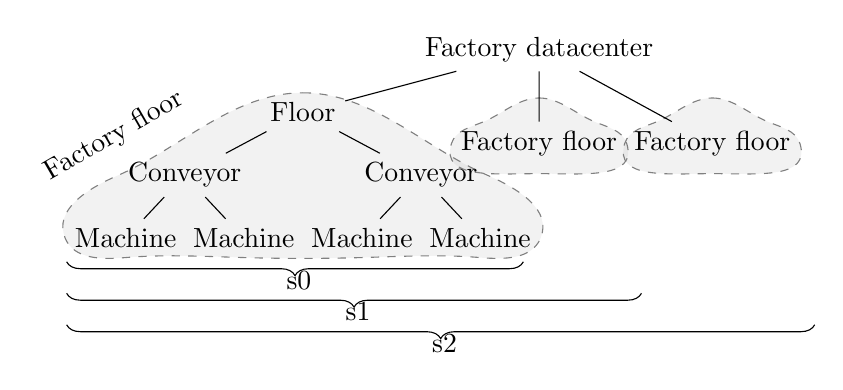
\begin{tikzpicture}[level distance=0.8cm]

	\tikzstyle{level 1}=[sibling distance=3cm]
	\tikzstyle{level 2}=[sibling distance=3cm]
	\tikzstyle{level 3}=[sibling distance=1.5cm]
	
	\node [rotate=30] (floorLabel) at (-5.4,-1.1) {Factory floor};
	%\draw[dashed] (floorLabel.south) -- (-4.5, -1.1);
	
	\node (d) {Factory datacenter}
		child {node (f1) {Floor}
			child { node (c1) {Conveyor} 
				child { node (m11) {Machine} }
				child { node (m12) {Machine} }	
			}
			child { node (c2) {Conveyor}
				child { node (m21) {Machine} }
				child { node (m22) {Machine} }
			}
		}
		child[level distance=1.2cm] {node (f2) {Factory floor}}
		child[level distance=1.2cm, sibling distance=2.2cm] {node (f3) {Factory floor}};
	
	\begin{pgfonlayer}{background}
	\draw[gray,fill=gray,dashed,fill opacity=0.1](f1.north) 
	to[closed,curve through={(c2.east).. (m22.east) .. (m22.south) .. (m21.south) .. (m12.south)
		.. (m11.south).. (m11.west) .. (c1.west) }](f1.north);
	\end{pgfonlayer}
	
	\begin{pgfonlayer}{background}
	\draw[gray,fill=gray,dashed,fill opacity=0.1]([yshift=0.3cm]f2.north) 
	to[closed,curve through={([xshift=0.7cm]f2.north) .. (f2.east) .. ([yshift=-0.1cm]f2.south) .. (f2.west) .. ([xshift=-0.7cm]f2.north)}]([yshift=0.3cm]f2.north);
	\end{pgfonlayer}
	
	\begin{pgfonlayer}{background}
	\draw[gray,fill=gray,dashed,fill opacity=0.1]([yshift=0.3cm]f3.north) 
	to[closed,curve through={([xshift=0.7cm]f3.north) .. (f3.east) .. ([yshift=-0.1cm]f3.south) .. (f3.west) .. ([xshift=-0.7cm]f3.north)}]([yshift=0.3cm]f3.north);
	\end{pgfonlayer}
	
	\draw[snake=brace, mirror snake, segment amplitude=5] (-6, -2.7) -- (-0.2, -2.7) node[midway,below, xshift=0.05cm]{s0};
	
	\draw[snake=brace, mirror snake, segment amplitude=5] (-6, -3.1) -- (1.3, -3.1) node[midway,below, xshift=0.05cm]{s1};
	
	\draw[snake=brace, mirror snake, segment amplitude=5] (-6, -3.5) -- (3.5, -3.5) node[midway,below, xshift=0.05cm]{s2};
	
\end{tikzpicture}
%\end{document}
	}
\end{figure}

\begin{table}
	\centering
	\caption{Machine hosts for scalability experiments}
	\label{tab:scala_hosts}
	\scalebox{0.92}{
		\begin{tabular}{|c|c|c|c|c|}
			\hline
			\textbf{Virtual node}		&Datacenter	&Floor			&Conveyor	&Machine \\ \hline
			\textbf{Physical host}&Server		&Raspberry Pi	&Server		&Laptop \\ \hline
		\end{tabular}
	}
\end{table}

\subsubsection{Results}

Due to scaling issues, results are separated in several figures: 
\begin{itemize}
	\item Results for centralized deduction delivery mechanisms (\textit{i.e.} \gls{cir} and \gls{cdr}) are shown on Fig. \ref{fig:factory_scala_raw_syn} for single-host execution, and on Fig. \ref{fig:factory_scala_raw_rpi} for multi-host execution.
	\item Results for distributed deduction delivery mechanisms (\textit{i.e.} \gls{cip}, \gls{cdp} and \gls{adp}), are shown on Fig. \ref{fig:scalability_processed_syn} for single-host execution, and on Fig. \ref{fig:scalability_processed_rpi} and \ref{fig:scalability_processed_rpi2} for multi-host execution.
\end{itemize}

\begin{figure*}
	\Centering
	\caption{Scalability measures, single-host execution}
	\label{fig:factory_scala_raw}
	\begin{minipage}{0.395\textwidth}
		\Centering
		\subcaption{Centralized reasoning}
		\label{fig:factory_scala_raw_syn}
		\scalebox{1}{
			%% Creator: Matplotlib, PGF backend
%%
%% To include the figure in your LaTeX document, write
%%   \input{<filename>.pgf}
%%
%% Make sure the required packages are loaded in your preamble
%%   \usepackage{pgf}
%%
%% Figures using additional raster images can only be included by \input if
%% they are in the same directory as the main LaTeX file. For loading figures
%% from other directories you can use the `import` package
%%   \usepackage{import}
%% and then include the figures with
%%   \import{<path to file>}{<filename>.pgf}
%%
%% Matplotlib used the following preamble
%%   \usepackage{fontspec}
%%   \setsansfont{DejaVu Sans}
%%   \setmonofont{DejaVu Sans Mono}
%%
\begingroup%
\makeatletter%
\begin{pgfpicture}%
\pgfpathrectangle{\pgfpointorigin}{\pgfqpoint{2.500000in}{1.700000in}}%
\pgfusepath{use as bounding box, clip}%
\begin{pgfscope}%
\pgfsetbuttcap%
\pgfsetmiterjoin%
\definecolor{currentfill}{rgb}{1.000000,1.000000,1.000000}%
\pgfsetfillcolor{currentfill}%
\pgfsetlinewidth{0.000000pt}%
\definecolor{currentstroke}{rgb}{1.000000,1.000000,1.000000}%
\pgfsetstrokecolor{currentstroke}%
\pgfsetdash{}{0pt}%
\pgfpathmoveto{\pgfqpoint{0.000000in}{0.000000in}}%
\pgfpathlineto{\pgfqpoint{2.500000in}{0.000000in}}%
\pgfpathlineto{\pgfqpoint{2.500000in}{1.700000in}}%
\pgfpathlineto{\pgfqpoint{0.000000in}{1.700000in}}%
\pgfpathclose%
\pgfusepath{fill}%
\end{pgfscope}%
\begin{pgfscope}%
\pgfsetbuttcap%
\pgfsetmiterjoin%
\definecolor{currentfill}{rgb}{1.000000,1.000000,1.000000}%
\pgfsetfillcolor{currentfill}%
\pgfsetlinewidth{0.000000pt}%
\definecolor{currentstroke}{rgb}{0.000000,0.000000,0.000000}%
\pgfsetstrokecolor{currentstroke}%
\pgfsetstrokeopacity{0.000000}%
\pgfsetdash{}{0pt}%
\pgfpathmoveto{\pgfqpoint{0.575000in}{0.357000in}}%
\pgfpathlineto{\pgfqpoint{2.475000in}{0.357000in}}%
\pgfpathlineto{\pgfqpoint{2.475000in}{1.666000in}}%
\pgfpathlineto{\pgfqpoint{0.575000in}{1.666000in}}%
\pgfpathclose%
\pgfusepath{fill}%
\end{pgfscope}%
\begin{pgfscope}%
\pgfsetbuttcap%
\pgfsetroundjoin%
\definecolor{currentfill}{rgb}{0.000000,0.000000,0.000000}%
\pgfsetfillcolor{currentfill}%
\pgfsetlinewidth{0.803000pt}%
\definecolor{currentstroke}{rgb}{0.000000,0.000000,0.000000}%
\pgfsetstrokecolor{currentstroke}%
\pgfsetdash{}{0pt}%
\pgfsys@defobject{currentmarker}{\pgfqpoint{0.000000in}{-0.048611in}}{\pgfqpoint{0.000000in}{0.000000in}}{%
\pgfpathmoveto{\pgfqpoint{0.000000in}{0.000000in}}%
\pgfpathlineto{\pgfqpoint{0.000000in}{-0.048611in}}%
\pgfusepath{stroke,fill}%
}%
\begin{pgfscope}%
\pgfsys@transformshift{0.733333in}{0.357000in}%
\pgfsys@useobject{currentmarker}{}%
\end{pgfscope}%
\end{pgfscope}%
\begin{pgfscope}%
\pgftext[x=0.651944in,y=0.163389in,left,base]{\rmfamily\fontsize{10.000000}{12.000000}\selectfont s'0}%
\end{pgfscope}%
\begin{pgfscope}%
\pgftext[x=0.655972in,y=0.020778in,left,base]{\rmfamily\fontsize{10.000000}{12.000000}\selectfont cir}%
\end{pgfscope}%
\begin{pgfscope}%
\pgfsetbuttcap%
\pgfsetroundjoin%
\definecolor{currentfill}{rgb}{0.000000,0.000000,0.000000}%
\pgfsetfillcolor{currentfill}%
\pgfsetlinewidth{0.803000pt}%
\definecolor{currentstroke}{rgb}{0.000000,0.000000,0.000000}%
\pgfsetstrokecolor{currentstroke}%
\pgfsetdash{}{0pt}%
\pgfsys@defobject{currentmarker}{\pgfqpoint{0.000000in}{-0.048611in}}{\pgfqpoint{0.000000in}{0.000000in}}{%
\pgfpathmoveto{\pgfqpoint{0.000000in}{0.000000in}}%
\pgfpathlineto{\pgfqpoint{0.000000in}{-0.048611in}}%
\pgfusepath{stroke,fill}%
}%
\begin{pgfscope}%
\pgfsys@transformshift{1.050000in}{0.357000in}%
\pgfsys@useobject{currentmarker}{}%
\end{pgfscope}%
\end{pgfscope}%
\begin{pgfscope}%
\pgftext[x=0.968611in,y=0.163389in,left,base]{\rmfamily\fontsize{10.000000}{12.000000}\selectfont s'1}%
\end{pgfscope}%
\begin{pgfscope}%
\pgftext[x=0.972639in,y=0.020778in,left,base]{\rmfamily\fontsize{10.000000}{12.000000}\selectfont cir}%
\end{pgfscope}%
\begin{pgfscope}%
\pgfsetbuttcap%
\pgfsetroundjoin%
\definecolor{currentfill}{rgb}{0.000000,0.000000,0.000000}%
\pgfsetfillcolor{currentfill}%
\pgfsetlinewidth{0.803000pt}%
\definecolor{currentstroke}{rgb}{0.000000,0.000000,0.000000}%
\pgfsetstrokecolor{currentstroke}%
\pgfsetdash{}{0pt}%
\pgfsys@defobject{currentmarker}{\pgfqpoint{0.000000in}{-0.048611in}}{\pgfqpoint{0.000000in}{0.000000in}}{%
\pgfpathmoveto{\pgfqpoint{0.000000in}{0.000000in}}%
\pgfpathlineto{\pgfqpoint{0.000000in}{-0.048611in}}%
\pgfusepath{stroke,fill}%
}%
\begin{pgfscope}%
\pgfsys@transformshift{1.366667in}{0.357000in}%
\pgfsys@useobject{currentmarker}{}%
\end{pgfscope}%
\end{pgfscope}%
\begin{pgfscope}%
\pgftext[x=1.285278in,y=0.163389in,left,base]{\rmfamily\fontsize{10.000000}{12.000000}\selectfont s'2}%
\end{pgfscope}%
\begin{pgfscope}%
\pgftext[x=1.289306in,y=0.020778in,left,base]{\rmfamily\fontsize{10.000000}{12.000000}\selectfont cir}%
\end{pgfscope}%
\begin{pgfscope}%
\pgfsetbuttcap%
\pgfsetroundjoin%
\definecolor{currentfill}{rgb}{0.000000,0.000000,0.000000}%
\pgfsetfillcolor{currentfill}%
\pgfsetlinewidth{0.803000pt}%
\definecolor{currentstroke}{rgb}{0.000000,0.000000,0.000000}%
\pgfsetstrokecolor{currentstroke}%
\pgfsetdash{}{0pt}%
\pgfsys@defobject{currentmarker}{\pgfqpoint{0.000000in}{-0.048611in}}{\pgfqpoint{0.000000in}{0.000000in}}{%
\pgfpathmoveto{\pgfqpoint{0.000000in}{0.000000in}}%
\pgfpathlineto{\pgfqpoint{0.000000in}{-0.048611in}}%
\pgfusepath{stroke,fill}%
}%
\begin{pgfscope}%
\pgfsys@transformshift{1.683333in}{0.357000in}%
\pgfsys@useobject{currentmarker}{}%
\end{pgfscope}%
\end{pgfscope}%
\begin{pgfscope}%
\pgftext[x=1.601944in,y=0.163389in,left,base]{\rmfamily\fontsize{10.000000}{12.000000}\selectfont s'0}%
\end{pgfscope}%
\begin{pgfscope}%
\pgftext[x=1.586667in,y=0.020778in,left,base]{\rmfamily\fontsize{10.000000}{12.000000}\selectfont cdr}%
\end{pgfscope}%
\begin{pgfscope}%
\pgfsetbuttcap%
\pgfsetroundjoin%
\definecolor{currentfill}{rgb}{0.000000,0.000000,0.000000}%
\pgfsetfillcolor{currentfill}%
\pgfsetlinewidth{0.803000pt}%
\definecolor{currentstroke}{rgb}{0.000000,0.000000,0.000000}%
\pgfsetstrokecolor{currentstroke}%
\pgfsetdash{}{0pt}%
\pgfsys@defobject{currentmarker}{\pgfqpoint{0.000000in}{-0.048611in}}{\pgfqpoint{0.000000in}{0.000000in}}{%
\pgfpathmoveto{\pgfqpoint{0.000000in}{0.000000in}}%
\pgfpathlineto{\pgfqpoint{0.000000in}{-0.048611in}}%
\pgfusepath{stroke,fill}%
}%
\begin{pgfscope}%
\pgfsys@transformshift{2.000000in}{0.357000in}%
\pgfsys@useobject{currentmarker}{}%
\end{pgfscope}%
\end{pgfscope}%
\begin{pgfscope}%
\pgftext[x=1.918611in,y=0.163389in,left,base]{\rmfamily\fontsize{10.000000}{12.000000}\selectfont s'1}%
\end{pgfscope}%
\begin{pgfscope}%
\pgftext[x=1.903333in,y=0.020778in,left,base]{\rmfamily\fontsize{10.000000}{12.000000}\selectfont cdr}%
\end{pgfscope}%
\begin{pgfscope}%
\pgfsetbuttcap%
\pgfsetroundjoin%
\definecolor{currentfill}{rgb}{0.000000,0.000000,0.000000}%
\pgfsetfillcolor{currentfill}%
\pgfsetlinewidth{0.803000pt}%
\definecolor{currentstroke}{rgb}{0.000000,0.000000,0.000000}%
\pgfsetstrokecolor{currentstroke}%
\pgfsetdash{}{0pt}%
\pgfsys@defobject{currentmarker}{\pgfqpoint{0.000000in}{-0.048611in}}{\pgfqpoint{0.000000in}{0.000000in}}{%
\pgfpathmoveto{\pgfqpoint{0.000000in}{0.000000in}}%
\pgfpathlineto{\pgfqpoint{0.000000in}{-0.048611in}}%
\pgfusepath{stroke,fill}%
}%
\begin{pgfscope}%
\pgfsys@transformshift{2.316667in}{0.357000in}%
\pgfsys@useobject{currentmarker}{}%
\end{pgfscope}%
\end{pgfscope}%
\begin{pgfscope}%
\pgftext[x=2.235278in,y=0.163389in,left,base]{\rmfamily\fontsize{10.000000}{12.000000}\selectfont s'2}%
\end{pgfscope}%
\begin{pgfscope}%
\pgftext[x=2.220000in,y=0.020778in,left,base]{\rmfamily\fontsize{10.000000}{12.000000}\selectfont cdr}%
\end{pgfscope}%
\begin{pgfscope}%
\pgfpathrectangle{\pgfqpoint{0.575000in}{0.357000in}}{\pgfqpoint{1.900000in}{1.309000in}} %
\pgfusepath{clip}%
\pgfsetbuttcap%
\pgfsetroundjoin%
\pgfsetlinewidth{0.803000pt}%
\definecolor{currentstroke}{rgb}{0.690196,0.690196,0.690196}%
\pgfsetstrokecolor{currentstroke}%
\pgfsetdash{{2.960000pt}{1.280000pt}}{0.000000pt}%
\pgfpathmoveto{\pgfqpoint{0.575000in}{0.415080in}}%
\pgfpathlineto{\pgfqpoint{2.475000in}{0.415080in}}%
\pgfusepath{stroke}%
\end{pgfscope}%
\begin{pgfscope}%
\pgfsetbuttcap%
\pgfsetroundjoin%
\definecolor{currentfill}{rgb}{0.000000,0.000000,0.000000}%
\pgfsetfillcolor{currentfill}%
\pgfsetlinewidth{0.803000pt}%
\definecolor{currentstroke}{rgb}{0.000000,0.000000,0.000000}%
\pgfsetstrokecolor{currentstroke}%
\pgfsetdash{}{0pt}%
\pgfsys@defobject{currentmarker}{\pgfqpoint{-0.048611in}{0.000000in}}{\pgfqpoint{0.000000in}{0.000000in}}{%
\pgfpathmoveto{\pgfqpoint{0.000000in}{0.000000in}}%
\pgfpathlineto{\pgfqpoint{-0.048611in}{0.000000in}}%
\pgfusepath{stroke,fill}%
}%
\begin{pgfscope}%
\pgfsys@transformshift{0.575000in}{0.415080in}%
\pgfsys@useobject{currentmarker}{}%
\end{pgfscope}%
\end{pgfscope}%
\begin{pgfscope}%
\pgftext[x=0.408333in,y=0.366886in,left,base]{\rmfamily\fontsize{10.000000}{12.000000}\selectfont \(\displaystyle 0\)}%
\end{pgfscope}%
\begin{pgfscope}%
\pgfpathrectangle{\pgfqpoint{0.575000in}{0.357000in}}{\pgfqpoint{1.900000in}{1.309000in}} %
\pgfusepath{clip}%
\pgfsetbuttcap%
\pgfsetroundjoin%
\pgfsetlinewidth{0.803000pt}%
\definecolor{currentstroke}{rgb}{0.690196,0.690196,0.690196}%
\pgfsetstrokecolor{currentstroke}%
\pgfsetdash{{2.960000pt}{1.280000pt}}{0.000000pt}%
\pgfpathmoveto{\pgfqpoint{0.575000in}{0.537488in}}%
\pgfpathlineto{\pgfqpoint{2.475000in}{0.537488in}}%
\pgfusepath{stroke}%
\end{pgfscope}%
\begin{pgfscope}%
\pgfsetbuttcap%
\pgfsetroundjoin%
\definecolor{currentfill}{rgb}{0.000000,0.000000,0.000000}%
\pgfsetfillcolor{currentfill}%
\pgfsetlinewidth{0.803000pt}%
\definecolor{currentstroke}{rgb}{0.000000,0.000000,0.000000}%
\pgfsetstrokecolor{currentstroke}%
\pgfsetdash{}{0pt}%
\pgfsys@defobject{currentmarker}{\pgfqpoint{-0.048611in}{0.000000in}}{\pgfqpoint{0.000000in}{0.000000in}}{%
\pgfpathmoveto{\pgfqpoint{0.000000in}{0.000000in}}%
\pgfpathlineto{\pgfqpoint{-0.048611in}{0.000000in}}%
\pgfusepath{stroke,fill}%
}%
\begin{pgfscope}%
\pgfsys@transformshift{0.575000in}{0.537488in}%
\pgfsys@useobject{currentmarker}{}%
\end{pgfscope}%
\end{pgfscope}%
\begin{pgfscope}%
\pgftext[x=0.408333in,y=0.489293in,left,base]{\rmfamily\fontsize{10.000000}{12.000000}\selectfont \(\displaystyle 5\)}%
\end{pgfscope}%
\begin{pgfscope}%
\pgfpathrectangle{\pgfqpoint{0.575000in}{0.357000in}}{\pgfqpoint{1.900000in}{1.309000in}} %
\pgfusepath{clip}%
\pgfsetbuttcap%
\pgfsetroundjoin%
\pgfsetlinewidth{0.803000pt}%
\definecolor{currentstroke}{rgb}{0.690196,0.690196,0.690196}%
\pgfsetstrokecolor{currentstroke}%
\pgfsetdash{{2.960000pt}{1.280000pt}}{0.000000pt}%
\pgfpathmoveto{\pgfqpoint{0.575000in}{0.659896in}}%
\pgfpathlineto{\pgfqpoint{2.475000in}{0.659896in}}%
\pgfusepath{stroke}%
\end{pgfscope}%
\begin{pgfscope}%
\pgfsetbuttcap%
\pgfsetroundjoin%
\definecolor{currentfill}{rgb}{0.000000,0.000000,0.000000}%
\pgfsetfillcolor{currentfill}%
\pgfsetlinewidth{0.803000pt}%
\definecolor{currentstroke}{rgb}{0.000000,0.000000,0.000000}%
\pgfsetstrokecolor{currentstroke}%
\pgfsetdash{}{0pt}%
\pgfsys@defobject{currentmarker}{\pgfqpoint{-0.048611in}{0.000000in}}{\pgfqpoint{0.000000in}{0.000000in}}{%
\pgfpathmoveto{\pgfqpoint{0.000000in}{0.000000in}}%
\pgfpathlineto{\pgfqpoint{-0.048611in}{0.000000in}}%
\pgfusepath{stroke,fill}%
}%
\begin{pgfscope}%
\pgfsys@transformshift{0.575000in}{0.659896in}%
\pgfsys@useobject{currentmarker}{}%
\end{pgfscope}%
\end{pgfscope}%
\begin{pgfscope}%
\pgftext[x=0.338888in,y=0.611701in,left,base]{\rmfamily\fontsize{10.000000}{12.000000}\selectfont \(\displaystyle 10\)}%
\end{pgfscope}%
\begin{pgfscope}%
\pgfpathrectangle{\pgfqpoint{0.575000in}{0.357000in}}{\pgfqpoint{1.900000in}{1.309000in}} %
\pgfusepath{clip}%
\pgfsetbuttcap%
\pgfsetroundjoin%
\pgfsetlinewidth{0.803000pt}%
\definecolor{currentstroke}{rgb}{0.690196,0.690196,0.690196}%
\pgfsetstrokecolor{currentstroke}%
\pgfsetdash{{2.960000pt}{1.280000pt}}{0.000000pt}%
\pgfpathmoveto{\pgfqpoint{0.575000in}{0.782304in}}%
\pgfpathlineto{\pgfqpoint{2.475000in}{0.782304in}}%
\pgfusepath{stroke}%
\end{pgfscope}%
\begin{pgfscope}%
\pgfsetbuttcap%
\pgfsetroundjoin%
\definecolor{currentfill}{rgb}{0.000000,0.000000,0.000000}%
\pgfsetfillcolor{currentfill}%
\pgfsetlinewidth{0.803000pt}%
\definecolor{currentstroke}{rgb}{0.000000,0.000000,0.000000}%
\pgfsetstrokecolor{currentstroke}%
\pgfsetdash{}{0pt}%
\pgfsys@defobject{currentmarker}{\pgfqpoint{-0.048611in}{0.000000in}}{\pgfqpoint{0.000000in}{0.000000in}}{%
\pgfpathmoveto{\pgfqpoint{0.000000in}{0.000000in}}%
\pgfpathlineto{\pgfqpoint{-0.048611in}{0.000000in}}%
\pgfusepath{stroke,fill}%
}%
\begin{pgfscope}%
\pgfsys@transformshift{0.575000in}{0.782304in}%
\pgfsys@useobject{currentmarker}{}%
\end{pgfscope}%
\end{pgfscope}%
\begin{pgfscope}%
\pgftext[x=0.338888in,y=0.734109in,left,base]{\rmfamily\fontsize{10.000000}{12.000000}\selectfont \(\displaystyle 15\)}%
\end{pgfscope}%
\begin{pgfscope}%
\pgfpathrectangle{\pgfqpoint{0.575000in}{0.357000in}}{\pgfqpoint{1.900000in}{1.309000in}} %
\pgfusepath{clip}%
\pgfsetbuttcap%
\pgfsetroundjoin%
\pgfsetlinewidth{0.803000pt}%
\definecolor{currentstroke}{rgb}{0.690196,0.690196,0.690196}%
\pgfsetstrokecolor{currentstroke}%
\pgfsetdash{{2.960000pt}{1.280000pt}}{0.000000pt}%
\pgfpathmoveto{\pgfqpoint{0.575000in}{0.904711in}}%
\pgfpathlineto{\pgfqpoint{2.475000in}{0.904711in}}%
\pgfusepath{stroke}%
\end{pgfscope}%
\begin{pgfscope}%
\pgfsetbuttcap%
\pgfsetroundjoin%
\definecolor{currentfill}{rgb}{0.000000,0.000000,0.000000}%
\pgfsetfillcolor{currentfill}%
\pgfsetlinewidth{0.803000pt}%
\definecolor{currentstroke}{rgb}{0.000000,0.000000,0.000000}%
\pgfsetstrokecolor{currentstroke}%
\pgfsetdash{}{0pt}%
\pgfsys@defobject{currentmarker}{\pgfqpoint{-0.048611in}{0.000000in}}{\pgfqpoint{0.000000in}{0.000000in}}{%
\pgfpathmoveto{\pgfqpoint{0.000000in}{0.000000in}}%
\pgfpathlineto{\pgfqpoint{-0.048611in}{0.000000in}}%
\pgfusepath{stroke,fill}%
}%
\begin{pgfscope}%
\pgfsys@transformshift{0.575000in}{0.904711in}%
\pgfsys@useobject{currentmarker}{}%
\end{pgfscope}%
\end{pgfscope}%
\begin{pgfscope}%
\pgftext[x=0.338888in,y=0.856517in,left,base]{\rmfamily\fontsize{10.000000}{12.000000}\selectfont \(\displaystyle 20\)}%
\end{pgfscope}%
\begin{pgfscope}%
\pgfpathrectangle{\pgfqpoint{0.575000in}{0.357000in}}{\pgfqpoint{1.900000in}{1.309000in}} %
\pgfusepath{clip}%
\pgfsetbuttcap%
\pgfsetroundjoin%
\pgfsetlinewidth{0.803000pt}%
\definecolor{currentstroke}{rgb}{0.690196,0.690196,0.690196}%
\pgfsetstrokecolor{currentstroke}%
\pgfsetdash{{2.960000pt}{1.280000pt}}{0.000000pt}%
\pgfpathmoveto{\pgfqpoint{0.575000in}{1.027119in}}%
\pgfpathlineto{\pgfqpoint{2.475000in}{1.027119in}}%
\pgfusepath{stroke}%
\end{pgfscope}%
\begin{pgfscope}%
\pgfsetbuttcap%
\pgfsetroundjoin%
\definecolor{currentfill}{rgb}{0.000000,0.000000,0.000000}%
\pgfsetfillcolor{currentfill}%
\pgfsetlinewidth{0.803000pt}%
\definecolor{currentstroke}{rgb}{0.000000,0.000000,0.000000}%
\pgfsetstrokecolor{currentstroke}%
\pgfsetdash{}{0pt}%
\pgfsys@defobject{currentmarker}{\pgfqpoint{-0.048611in}{0.000000in}}{\pgfqpoint{0.000000in}{0.000000in}}{%
\pgfpathmoveto{\pgfqpoint{0.000000in}{0.000000in}}%
\pgfpathlineto{\pgfqpoint{-0.048611in}{0.000000in}}%
\pgfusepath{stroke,fill}%
}%
\begin{pgfscope}%
\pgfsys@transformshift{0.575000in}{1.027119in}%
\pgfsys@useobject{currentmarker}{}%
\end{pgfscope}%
\end{pgfscope}%
\begin{pgfscope}%
\pgftext[x=0.338888in,y=0.978925in,left,base]{\rmfamily\fontsize{10.000000}{12.000000}\selectfont \(\displaystyle 25\)}%
\end{pgfscope}%
\begin{pgfscope}%
\pgfpathrectangle{\pgfqpoint{0.575000in}{0.357000in}}{\pgfqpoint{1.900000in}{1.309000in}} %
\pgfusepath{clip}%
\pgfsetbuttcap%
\pgfsetroundjoin%
\pgfsetlinewidth{0.803000pt}%
\definecolor{currentstroke}{rgb}{0.690196,0.690196,0.690196}%
\pgfsetstrokecolor{currentstroke}%
\pgfsetdash{{2.960000pt}{1.280000pt}}{0.000000pt}%
\pgfpathmoveto{\pgfqpoint{0.575000in}{1.149527in}}%
\pgfpathlineto{\pgfqpoint{2.475000in}{1.149527in}}%
\pgfusepath{stroke}%
\end{pgfscope}%
\begin{pgfscope}%
\pgfsetbuttcap%
\pgfsetroundjoin%
\definecolor{currentfill}{rgb}{0.000000,0.000000,0.000000}%
\pgfsetfillcolor{currentfill}%
\pgfsetlinewidth{0.803000pt}%
\definecolor{currentstroke}{rgb}{0.000000,0.000000,0.000000}%
\pgfsetstrokecolor{currentstroke}%
\pgfsetdash{}{0pt}%
\pgfsys@defobject{currentmarker}{\pgfqpoint{-0.048611in}{0.000000in}}{\pgfqpoint{0.000000in}{0.000000in}}{%
\pgfpathmoveto{\pgfqpoint{0.000000in}{0.000000in}}%
\pgfpathlineto{\pgfqpoint{-0.048611in}{0.000000in}}%
\pgfusepath{stroke,fill}%
}%
\begin{pgfscope}%
\pgfsys@transformshift{0.575000in}{1.149527in}%
\pgfsys@useobject{currentmarker}{}%
\end{pgfscope}%
\end{pgfscope}%
\begin{pgfscope}%
\pgftext[x=0.338888in,y=1.101333in,left,base]{\rmfamily\fontsize{10.000000}{12.000000}\selectfont \(\displaystyle 30\)}%
\end{pgfscope}%
\begin{pgfscope}%
\pgfpathrectangle{\pgfqpoint{0.575000in}{0.357000in}}{\pgfqpoint{1.900000in}{1.309000in}} %
\pgfusepath{clip}%
\pgfsetbuttcap%
\pgfsetroundjoin%
\pgfsetlinewidth{0.803000pt}%
\definecolor{currentstroke}{rgb}{0.690196,0.690196,0.690196}%
\pgfsetstrokecolor{currentstroke}%
\pgfsetdash{{2.960000pt}{1.280000pt}}{0.000000pt}%
\pgfpathmoveto{\pgfqpoint{0.575000in}{1.271935in}}%
\pgfpathlineto{\pgfqpoint{2.475000in}{1.271935in}}%
\pgfusepath{stroke}%
\end{pgfscope}%
\begin{pgfscope}%
\pgfsetbuttcap%
\pgfsetroundjoin%
\definecolor{currentfill}{rgb}{0.000000,0.000000,0.000000}%
\pgfsetfillcolor{currentfill}%
\pgfsetlinewidth{0.803000pt}%
\definecolor{currentstroke}{rgb}{0.000000,0.000000,0.000000}%
\pgfsetstrokecolor{currentstroke}%
\pgfsetdash{}{0pt}%
\pgfsys@defobject{currentmarker}{\pgfqpoint{-0.048611in}{0.000000in}}{\pgfqpoint{0.000000in}{0.000000in}}{%
\pgfpathmoveto{\pgfqpoint{0.000000in}{0.000000in}}%
\pgfpathlineto{\pgfqpoint{-0.048611in}{0.000000in}}%
\pgfusepath{stroke,fill}%
}%
\begin{pgfscope}%
\pgfsys@transformshift{0.575000in}{1.271935in}%
\pgfsys@useobject{currentmarker}{}%
\end{pgfscope}%
\end{pgfscope}%
\begin{pgfscope}%
\pgftext[x=0.338888in,y=1.223740in,left,base]{\rmfamily\fontsize{10.000000}{12.000000}\selectfont \(\displaystyle 35\)}%
\end{pgfscope}%
\begin{pgfscope}%
\pgfpathrectangle{\pgfqpoint{0.575000in}{0.357000in}}{\pgfqpoint{1.900000in}{1.309000in}} %
\pgfusepath{clip}%
\pgfsetbuttcap%
\pgfsetroundjoin%
\pgfsetlinewidth{0.803000pt}%
\definecolor{currentstroke}{rgb}{0.690196,0.690196,0.690196}%
\pgfsetstrokecolor{currentstroke}%
\pgfsetdash{{2.960000pt}{1.280000pt}}{0.000000pt}%
\pgfpathmoveto{\pgfqpoint{0.575000in}{1.394343in}}%
\pgfpathlineto{\pgfqpoint{2.475000in}{1.394343in}}%
\pgfusepath{stroke}%
\end{pgfscope}%
\begin{pgfscope}%
\pgfsetbuttcap%
\pgfsetroundjoin%
\definecolor{currentfill}{rgb}{0.000000,0.000000,0.000000}%
\pgfsetfillcolor{currentfill}%
\pgfsetlinewidth{0.803000pt}%
\definecolor{currentstroke}{rgb}{0.000000,0.000000,0.000000}%
\pgfsetstrokecolor{currentstroke}%
\pgfsetdash{}{0pt}%
\pgfsys@defobject{currentmarker}{\pgfqpoint{-0.048611in}{0.000000in}}{\pgfqpoint{0.000000in}{0.000000in}}{%
\pgfpathmoveto{\pgfqpoint{0.000000in}{0.000000in}}%
\pgfpathlineto{\pgfqpoint{-0.048611in}{0.000000in}}%
\pgfusepath{stroke,fill}%
}%
\begin{pgfscope}%
\pgfsys@transformshift{0.575000in}{1.394343in}%
\pgfsys@useobject{currentmarker}{}%
\end{pgfscope}%
\end{pgfscope}%
\begin{pgfscope}%
\pgftext[x=0.338888in,y=1.346148in,left,base]{\rmfamily\fontsize{10.000000}{12.000000}\selectfont \(\displaystyle 40\)}%
\end{pgfscope}%
\begin{pgfscope}%
\pgfpathrectangle{\pgfqpoint{0.575000in}{0.357000in}}{\pgfqpoint{1.900000in}{1.309000in}} %
\pgfusepath{clip}%
\pgfsetbuttcap%
\pgfsetroundjoin%
\pgfsetlinewidth{0.803000pt}%
\definecolor{currentstroke}{rgb}{0.690196,0.690196,0.690196}%
\pgfsetstrokecolor{currentstroke}%
\pgfsetdash{{2.960000pt}{1.280000pt}}{0.000000pt}%
\pgfpathmoveto{\pgfqpoint{0.575000in}{1.516751in}}%
\pgfpathlineto{\pgfqpoint{2.475000in}{1.516751in}}%
\pgfusepath{stroke}%
\end{pgfscope}%
\begin{pgfscope}%
\pgfsetbuttcap%
\pgfsetroundjoin%
\definecolor{currentfill}{rgb}{0.000000,0.000000,0.000000}%
\pgfsetfillcolor{currentfill}%
\pgfsetlinewidth{0.803000pt}%
\definecolor{currentstroke}{rgb}{0.000000,0.000000,0.000000}%
\pgfsetstrokecolor{currentstroke}%
\pgfsetdash{}{0pt}%
\pgfsys@defobject{currentmarker}{\pgfqpoint{-0.048611in}{0.000000in}}{\pgfqpoint{0.000000in}{0.000000in}}{%
\pgfpathmoveto{\pgfqpoint{0.000000in}{0.000000in}}%
\pgfpathlineto{\pgfqpoint{-0.048611in}{0.000000in}}%
\pgfusepath{stroke,fill}%
}%
\begin{pgfscope}%
\pgfsys@transformshift{0.575000in}{1.516751in}%
\pgfsys@useobject{currentmarker}{}%
\end{pgfscope}%
\end{pgfscope}%
\begin{pgfscope}%
\pgftext[x=0.338888in,y=1.468556in,left,base]{\rmfamily\fontsize{10.000000}{12.000000}\selectfont \(\displaystyle 45\)}%
\end{pgfscope}%
\begin{pgfscope}%
\pgfpathrectangle{\pgfqpoint{0.575000in}{0.357000in}}{\pgfqpoint{1.900000in}{1.309000in}} %
\pgfusepath{clip}%
\pgfsetbuttcap%
\pgfsetroundjoin%
\pgfsetlinewidth{0.803000pt}%
\definecolor{currentstroke}{rgb}{0.690196,0.690196,0.690196}%
\pgfsetstrokecolor{currentstroke}%
\pgfsetdash{{2.960000pt}{1.280000pt}}{0.000000pt}%
\pgfpathmoveto{\pgfqpoint{0.575000in}{1.639158in}}%
\pgfpathlineto{\pgfqpoint{2.475000in}{1.639158in}}%
\pgfusepath{stroke}%
\end{pgfscope}%
\begin{pgfscope}%
\pgfsetbuttcap%
\pgfsetroundjoin%
\definecolor{currentfill}{rgb}{0.000000,0.000000,0.000000}%
\pgfsetfillcolor{currentfill}%
\pgfsetlinewidth{0.803000pt}%
\definecolor{currentstroke}{rgb}{0.000000,0.000000,0.000000}%
\pgfsetstrokecolor{currentstroke}%
\pgfsetdash{}{0pt}%
\pgfsys@defobject{currentmarker}{\pgfqpoint{-0.048611in}{0.000000in}}{\pgfqpoint{0.000000in}{0.000000in}}{%
\pgfpathmoveto{\pgfqpoint{0.000000in}{0.000000in}}%
\pgfpathlineto{\pgfqpoint{-0.048611in}{0.000000in}}%
\pgfusepath{stroke,fill}%
}%
\begin{pgfscope}%
\pgfsys@transformshift{0.575000in}{1.639158in}%
\pgfsys@useobject{currentmarker}{}%
\end{pgfscope}%
\end{pgfscope}%
\begin{pgfscope}%
\pgftext[x=0.338888in,y=1.590964in,left,base]{\rmfamily\fontsize{10.000000}{12.000000}\selectfont \(\displaystyle 50\)}%
\end{pgfscope}%
\begin{pgfscope}%
\pgfpathrectangle{\pgfqpoint{0.575000in}{0.357000in}}{\pgfqpoint{1.900000in}{1.309000in}} %
\pgfusepath{clip}%
\pgfsetbuttcap%
\pgfsetroundjoin%
\pgfsetlinewidth{0.803000pt}%
\definecolor{currentstroke}{rgb}{0.690196,0.690196,0.690196}%
\pgfsetstrokecolor{currentstroke}%
\pgfsetdash{{0.800000pt}{1.320000pt}}{0.000000pt}%
\pgfpathmoveto{\pgfqpoint{0.575000in}{0.415080in}}%
\pgfpathlineto{\pgfqpoint{2.475000in}{0.415080in}}%
\pgfusepath{stroke}%
\end{pgfscope}%
\begin{pgfscope}%
\pgfsetbuttcap%
\pgfsetroundjoin%
\definecolor{currentfill}{rgb}{0.000000,0.000000,0.000000}%
\pgfsetfillcolor{currentfill}%
\pgfsetlinewidth{0.602250pt}%
\definecolor{currentstroke}{rgb}{0.000000,0.000000,0.000000}%
\pgfsetstrokecolor{currentstroke}%
\pgfsetdash{}{0pt}%
\pgfsys@defobject{currentmarker}{\pgfqpoint{-0.027778in}{0.000000in}}{\pgfqpoint{0.000000in}{0.000000in}}{%
\pgfpathmoveto{\pgfqpoint{0.000000in}{0.000000in}}%
\pgfpathlineto{\pgfqpoint{-0.027778in}{0.000000in}}%
\pgfusepath{stroke,fill}%
}%
\begin{pgfscope}%
\pgfsys@transformshift{0.575000in}{0.415080in}%
\pgfsys@useobject{currentmarker}{}%
\end{pgfscope}%
\end{pgfscope}%
\begin{pgfscope}%
\pgfpathrectangle{\pgfqpoint{0.575000in}{0.357000in}}{\pgfqpoint{1.900000in}{1.309000in}} %
\pgfusepath{clip}%
\pgfsetbuttcap%
\pgfsetroundjoin%
\pgfsetlinewidth{0.803000pt}%
\definecolor{currentstroke}{rgb}{0.690196,0.690196,0.690196}%
\pgfsetstrokecolor{currentstroke}%
\pgfsetdash{{0.800000pt}{1.320000pt}}{0.000000pt}%
\pgfpathmoveto{\pgfqpoint{0.575000in}{0.476284in}}%
\pgfpathlineto{\pgfqpoint{2.475000in}{0.476284in}}%
\pgfusepath{stroke}%
\end{pgfscope}%
\begin{pgfscope}%
\pgfsetbuttcap%
\pgfsetroundjoin%
\definecolor{currentfill}{rgb}{0.000000,0.000000,0.000000}%
\pgfsetfillcolor{currentfill}%
\pgfsetlinewidth{0.602250pt}%
\definecolor{currentstroke}{rgb}{0.000000,0.000000,0.000000}%
\pgfsetstrokecolor{currentstroke}%
\pgfsetdash{}{0pt}%
\pgfsys@defobject{currentmarker}{\pgfqpoint{-0.027778in}{0.000000in}}{\pgfqpoint{0.000000in}{0.000000in}}{%
\pgfpathmoveto{\pgfqpoint{0.000000in}{0.000000in}}%
\pgfpathlineto{\pgfqpoint{-0.027778in}{0.000000in}}%
\pgfusepath{stroke,fill}%
}%
\begin{pgfscope}%
\pgfsys@transformshift{0.575000in}{0.476284in}%
\pgfsys@useobject{currentmarker}{}%
\end{pgfscope}%
\end{pgfscope}%
\begin{pgfscope}%
\pgfpathrectangle{\pgfqpoint{0.575000in}{0.357000in}}{\pgfqpoint{1.900000in}{1.309000in}} %
\pgfusepath{clip}%
\pgfsetbuttcap%
\pgfsetroundjoin%
\pgfsetlinewidth{0.803000pt}%
\definecolor{currentstroke}{rgb}{0.690196,0.690196,0.690196}%
\pgfsetstrokecolor{currentstroke}%
\pgfsetdash{{0.800000pt}{1.320000pt}}{0.000000pt}%
\pgfpathmoveto{\pgfqpoint{0.575000in}{0.537488in}}%
\pgfpathlineto{\pgfqpoint{2.475000in}{0.537488in}}%
\pgfusepath{stroke}%
\end{pgfscope}%
\begin{pgfscope}%
\pgfsetbuttcap%
\pgfsetroundjoin%
\definecolor{currentfill}{rgb}{0.000000,0.000000,0.000000}%
\pgfsetfillcolor{currentfill}%
\pgfsetlinewidth{0.602250pt}%
\definecolor{currentstroke}{rgb}{0.000000,0.000000,0.000000}%
\pgfsetstrokecolor{currentstroke}%
\pgfsetdash{}{0pt}%
\pgfsys@defobject{currentmarker}{\pgfqpoint{-0.027778in}{0.000000in}}{\pgfqpoint{0.000000in}{0.000000in}}{%
\pgfpathmoveto{\pgfqpoint{0.000000in}{0.000000in}}%
\pgfpathlineto{\pgfqpoint{-0.027778in}{0.000000in}}%
\pgfusepath{stroke,fill}%
}%
\begin{pgfscope}%
\pgfsys@transformshift{0.575000in}{0.537488in}%
\pgfsys@useobject{currentmarker}{}%
\end{pgfscope}%
\end{pgfscope}%
\begin{pgfscope}%
\pgfpathrectangle{\pgfqpoint{0.575000in}{0.357000in}}{\pgfqpoint{1.900000in}{1.309000in}} %
\pgfusepath{clip}%
\pgfsetbuttcap%
\pgfsetroundjoin%
\pgfsetlinewidth{0.803000pt}%
\definecolor{currentstroke}{rgb}{0.690196,0.690196,0.690196}%
\pgfsetstrokecolor{currentstroke}%
\pgfsetdash{{0.800000pt}{1.320000pt}}{0.000000pt}%
\pgfpathmoveto{\pgfqpoint{0.575000in}{0.598692in}}%
\pgfpathlineto{\pgfqpoint{2.475000in}{0.598692in}}%
\pgfusepath{stroke}%
\end{pgfscope}%
\begin{pgfscope}%
\pgfsetbuttcap%
\pgfsetroundjoin%
\definecolor{currentfill}{rgb}{0.000000,0.000000,0.000000}%
\pgfsetfillcolor{currentfill}%
\pgfsetlinewidth{0.602250pt}%
\definecolor{currentstroke}{rgb}{0.000000,0.000000,0.000000}%
\pgfsetstrokecolor{currentstroke}%
\pgfsetdash{}{0pt}%
\pgfsys@defobject{currentmarker}{\pgfqpoint{-0.027778in}{0.000000in}}{\pgfqpoint{0.000000in}{0.000000in}}{%
\pgfpathmoveto{\pgfqpoint{0.000000in}{0.000000in}}%
\pgfpathlineto{\pgfqpoint{-0.027778in}{0.000000in}}%
\pgfusepath{stroke,fill}%
}%
\begin{pgfscope}%
\pgfsys@transformshift{0.575000in}{0.598692in}%
\pgfsys@useobject{currentmarker}{}%
\end{pgfscope}%
\end{pgfscope}%
\begin{pgfscope}%
\pgfpathrectangle{\pgfqpoint{0.575000in}{0.357000in}}{\pgfqpoint{1.900000in}{1.309000in}} %
\pgfusepath{clip}%
\pgfsetbuttcap%
\pgfsetroundjoin%
\pgfsetlinewidth{0.803000pt}%
\definecolor{currentstroke}{rgb}{0.690196,0.690196,0.690196}%
\pgfsetstrokecolor{currentstroke}%
\pgfsetdash{{0.800000pt}{1.320000pt}}{0.000000pt}%
\pgfpathmoveto{\pgfqpoint{0.575000in}{0.659896in}}%
\pgfpathlineto{\pgfqpoint{2.475000in}{0.659896in}}%
\pgfusepath{stroke}%
\end{pgfscope}%
\begin{pgfscope}%
\pgfsetbuttcap%
\pgfsetroundjoin%
\definecolor{currentfill}{rgb}{0.000000,0.000000,0.000000}%
\pgfsetfillcolor{currentfill}%
\pgfsetlinewidth{0.602250pt}%
\definecolor{currentstroke}{rgb}{0.000000,0.000000,0.000000}%
\pgfsetstrokecolor{currentstroke}%
\pgfsetdash{}{0pt}%
\pgfsys@defobject{currentmarker}{\pgfqpoint{-0.027778in}{0.000000in}}{\pgfqpoint{0.000000in}{0.000000in}}{%
\pgfpathmoveto{\pgfqpoint{0.000000in}{0.000000in}}%
\pgfpathlineto{\pgfqpoint{-0.027778in}{0.000000in}}%
\pgfusepath{stroke,fill}%
}%
\begin{pgfscope}%
\pgfsys@transformshift{0.575000in}{0.659896in}%
\pgfsys@useobject{currentmarker}{}%
\end{pgfscope}%
\end{pgfscope}%
\begin{pgfscope}%
\pgfpathrectangle{\pgfqpoint{0.575000in}{0.357000in}}{\pgfqpoint{1.900000in}{1.309000in}} %
\pgfusepath{clip}%
\pgfsetbuttcap%
\pgfsetroundjoin%
\pgfsetlinewidth{0.803000pt}%
\definecolor{currentstroke}{rgb}{0.690196,0.690196,0.690196}%
\pgfsetstrokecolor{currentstroke}%
\pgfsetdash{{0.800000pt}{1.320000pt}}{0.000000pt}%
\pgfpathmoveto{\pgfqpoint{0.575000in}{0.721100in}}%
\pgfpathlineto{\pgfqpoint{2.475000in}{0.721100in}}%
\pgfusepath{stroke}%
\end{pgfscope}%
\begin{pgfscope}%
\pgfsetbuttcap%
\pgfsetroundjoin%
\definecolor{currentfill}{rgb}{0.000000,0.000000,0.000000}%
\pgfsetfillcolor{currentfill}%
\pgfsetlinewidth{0.602250pt}%
\definecolor{currentstroke}{rgb}{0.000000,0.000000,0.000000}%
\pgfsetstrokecolor{currentstroke}%
\pgfsetdash{}{0pt}%
\pgfsys@defobject{currentmarker}{\pgfqpoint{-0.027778in}{0.000000in}}{\pgfqpoint{0.000000in}{0.000000in}}{%
\pgfpathmoveto{\pgfqpoint{0.000000in}{0.000000in}}%
\pgfpathlineto{\pgfqpoint{-0.027778in}{0.000000in}}%
\pgfusepath{stroke,fill}%
}%
\begin{pgfscope}%
\pgfsys@transformshift{0.575000in}{0.721100in}%
\pgfsys@useobject{currentmarker}{}%
\end{pgfscope}%
\end{pgfscope}%
\begin{pgfscope}%
\pgfpathrectangle{\pgfqpoint{0.575000in}{0.357000in}}{\pgfqpoint{1.900000in}{1.309000in}} %
\pgfusepath{clip}%
\pgfsetbuttcap%
\pgfsetroundjoin%
\pgfsetlinewidth{0.803000pt}%
\definecolor{currentstroke}{rgb}{0.690196,0.690196,0.690196}%
\pgfsetstrokecolor{currentstroke}%
\pgfsetdash{{0.800000pt}{1.320000pt}}{0.000000pt}%
\pgfpathmoveto{\pgfqpoint{0.575000in}{0.782304in}}%
\pgfpathlineto{\pgfqpoint{2.475000in}{0.782304in}}%
\pgfusepath{stroke}%
\end{pgfscope}%
\begin{pgfscope}%
\pgfsetbuttcap%
\pgfsetroundjoin%
\definecolor{currentfill}{rgb}{0.000000,0.000000,0.000000}%
\pgfsetfillcolor{currentfill}%
\pgfsetlinewidth{0.602250pt}%
\definecolor{currentstroke}{rgb}{0.000000,0.000000,0.000000}%
\pgfsetstrokecolor{currentstroke}%
\pgfsetdash{}{0pt}%
\pgfsys@defobject{currentmarker}{\pgfqpoint{-0.027778in}{0.000000in}}{\pgfqpoint{0.000000in}{0.000000in}}{%
\pgfpathmoveto{\pgfqpoint{0.000000in}{0.000000in}}%
\pgfpathlineto{\pgfqpoint{-0.027778in}{0.000000in}}%
\pgfusepath{stroke,fill}%
}%
\begin{pgfscope}%
\pgfsys@transformshift{0.575000in}{0.782304in}%
\pgfsys@useobject{currentmarker}{}%
\end{pgfscope}%
\end{pgfscope}%
\begin{pgfscope}%
\pgfpathrectangle{\pgfqpoint{0.575000in}{0.357000in}}{\pgfqpoint{1.900000in}{1.309000in}} %
\pgfusepath{clip}%
\pgfsetbuttcap%
\pgfsetroundjoin%
\pgfsetlinewidth{0.803000pt}%
\definecolor{currentstroke}{rgb}{0.690196,0.690196,0.690196}%
\pgfsetstrokecolor{currentstroke}%
\pgfsetdash{{0.800000pt}{1.320000pt}}{0.000000pt}%
\pgfpathmoveto{\pgfqpoint{0.575000in}{0.843507in}}%
\pgfpathlineto{\pgfqpoint{2.475000in}{0.843507in}}%
\pgfusepath{stroke}%
\end{pgfscope}%
\begin{pgfscope}%
\pgfsetbuttcap%
\pgfsetroundjoin%
\definecolor{currentfill}{rgb}{0.000000,0.000000,0.000000}%
\pgfsetfillcolor{currentfill}%
\pgfsetlinewidth{0.602250pt}%
\definecolor{currentstroke}{rgb}{0.000000,0.000000,0.000000}%
\pgfsetstrokecolor{currentstroke}%
\pgfsetdash{}{0pt}%
\pgfsys@defobject{currentmarker}{\pgfqpoint{-0.027778in}{0.000000in}}{\pgfqpoint{0.000000in}{0.000000in}}{%
\pgfpathmoveto{\pgfqpoint{0.000000in}{0.000000in}}%
\pgfpathlineto{\pgfqpoint{-0.027778in}{0.000000in}}%
\pgfusepath{stroke,fill}%
}%
\begin{pgfscope}%
\pgfsys@transformshift{0.575000in}{0.843507in}%
\pgfsys@useobject{currentmarker}{}%
\end{pgfscope}%
\end{pgfscope}%
\begin{pgfscope}%
\pgfpathrectangle{\pgfqpoint{0.575000in}{0.357000in}}{\pgfqpoint{1.900000in}{1.309000in}} %
\pgfusepath{clip}%
\pgfsetbuttcap%
\pgfsetroundjoin%
\pgfsetlinewidth{0.803000pt}%
\definecolor{currentstroke}{rgb}{0.690196,0.690196,0.690196}%
\pgfsetstrokecolor{currentstroke}%
\pgfsetdash{{0.800000pt}{1.320000pt}}{0.000000pt}%
\pgfpathmoveto{\pgfqpoint{0.575000in}{0.904711in}}%
\pgfpathlineto{\pgfqpoint{2.475000in}{0.904711in}}%
\pgfusepath{stroke}%
\end{pgfscope}%
\begin{pgfscope}%
\pgfsetbuttcap%
\pgfsetroundjoin%
\definecolor{currentfill}{rgb}{0.000000,0.000000,0.000000}%
\pgfsetfillcolor{currentfill}%
\pgfsetlinewidth{0.602250pt}%
\definecolor{currentstroke}{rgb}{0.000000,0.000000,0.000000}%
\pgfsetstrokecolor{currentstroke}%
\pgfsetdash{}{0pt}%
\pgfsys@defobject{currentmarker}{\pgfqpoint{-0.027778in}{0.000000in}}{\pgfqpoint{0.000000in}{0.000000in}}{%
\pgfpathmoveto{\pgfqpoint{0.000000in}{0.000000in}}%
\pgfpathlineto{\pgfqpoint{-0.027778in}{0.000000in}}%
\pgfusepath{stroke,fill}%
}%
\begin{pgfscope}%
\pgfsys@transformshift{0.575000in}{0.904711in}%
\pgfsys@useobject{currentmarker}{}%
\end{pgfscope}%
\end{pgfscope}%
\begin{pgfscope}%
\pgfpathrectangle{\pgfqpoint{0.575000in}{0.357000in}}{\pgfqpoint{1.900000in}{1.309000in}} %
\pgfusepath{clip}%
\pgfsetbuttcap%
\pgfsetroundjoin%
\pgfsetlinewidth{0.803000pt}%
\definecolor{currentstroke}{rgb}{0.690196,0.690196,0.690196}%
\pgfsetstrokecolor{currentstroke}%
\pgfsetdash{{0.800000pt}{1.320000pt}}{0.000000pt}%
\pgfpathmoveto{\pgfqpoint{0.575000in}{0.965915in}}%
\pgfpathlineto{\pgfqpoint{2.475000in}{0.965915in}}%
\pgfusepath{stroke}%
\end{pgfscope}%
\begin{pgfscope}%
\pgfsetbuttcap%
\pgfsetroundjoin%
\definecolor{currentfill}{rgb}{0.000000,0.000000,0.000000}%
\pgfsetfillcolor{currentfill}%
\pgfsetlinewidth{0.602250pt}%
\definecolor{currentstroke}{rgb}{0.000000,0.000000,0.000000}%
\pgfsetstrokecolor{currentstroke}%
\pgfsetdash{}{0pt}%
\pgfsys@defobject{currentmarker}{\pgfqpoint{-0.027778in}{0.000000in}}{\pgfqpoint{0.000000in}{0.000000in}}{%
\pgfpathmoveto{\pgfqpoint{0.000000in}{0.000000in}}%
\pgfpathlineto{\pgfqpoint{-0.027778in}{0.000000in}}%
\pgfusepath{stroke,fill}%
}%
\begin{pgfscope}%
\pgfsys@transformshift{0.575000in}{0.965915in}%
\pgfsys@useobject{currentmarker}{}%
\end{pgfscope}%
\end{pgfscope}%
\begin{pgfscope}%
\pgfpathrectangle{\pgfqpoint{0.575000in}{0.357000in}}{\pgfqpoint{1.900000in}{1.309000in}} %
\pgfusepath{clip}%
\pgfsetbuttcap%
\pgfsetroundjoin%
\pgfsetlinewidth{0.803000pt}%
\definecolor{currentstroke}{rgb}{0.690196,0.690196,0.690196}%
\pgfsetstrokecolor{currentstroke}%
\pgfsetdash{{0.800000pt}{1.320000pt}}{0.000000pt}%
\pgfpathmoveto{\pgfqpoint{0.575000in}{1.027119in}}%
\pgfpathlineto{\pgfqpoint{2.475000in}{1.027119in}}%
\pgfusepath{stroke}%
\end{pgfscope}%
\begin{pgfscope}%
\pgfsetbuttcap%
\pgfsetroundjoin%
\definecolor{currentfill}{rgb}{0.000000,0.000000,0.000000}%
\pgfsetfillcolor{currentfill}%
\pgfsetlinewidth{0.602250pt}%
\definecolor{currentstroke}{rgb}{0.000000,0.000000,0.000000}%
\pgfsetstrokecolor{currentstroke}%
\pgfsetdash{}{0pt}%
\pgfsys@defobject{currentmarker}{\pgfqpoint{-0.027778in}{0.000000in}}{\pgfqpoint{0.000000in}{0.000000in}}{%
\pgfpathmoveto{\pgfqpoint{0.000000in}{0.000000in}}%
\pgfpathlineto{\pgfqpoint{-0.027778in}{0.000000in}}%
\pgfusepath{stroke,fill}%
}%
\begin{pgfscope}%
\pgfsys@transformshift{0.575000in}{1.027119in}%
\pgfsys@useobject{currentmarker}{}%
\end{pgfscope}%
\end{pgfscope}%
\begin{pgfscope}%
\pgfpathrectangle{\pgfqpoint{0.575000in}{0.357000in}}{\pgfqpoint{1.900000in}{1.309000in}} %
\pgfusepath{clip}%
\pgfsetbuttcap%
\pgfsetroundjoin%
\pgfsetlinewidth{0.803000pt}%
\definecolor{currentstroke}{rgb}{0.690196,0.690196,0.690196}%
\pgfsetstrokecolor{currentstroke}%
\pgfsetdash{{0.800000pt}{1.320000pt}}{0.000000pt}%
\pgfpathmoveto{\pgfqpoint{0.575000in}{1.088323in}}%
\pgfpathlineto{\pgfqpoint{2.475000in}{1.088323in}}%
\pgfusepath{stroke}%
\end{pgfscope}%
\begin{pgfscope}%
\pgfsetbuttcap%
\pgfsetroundjoin%
\definecolor{currentfill}{rgb}{0.000000,0.000000,0.000000}%
\pgfsetfillcolor{currentfill}%
\pgfsetlinewidth{0.602250pt}%
\definecolor{currentstroke}{rgb}{0.000000,0.000000,0.000000}%
\pgfsetstrokecolor{currentstroke}%
\pgfsetdash{}{0pt}%
\pgfsys@defobject{currentmarker}{\pgfqpoint{-0.027778in}{0.000000in}}{\pgfqpoint{0.000000in}{0.000000in}}{%
\pgfpathmoveto{\pgfqpoint{0.000000in}{0.000000in}}%
\pgfpathlineto{\pgfqpoint{-0.027778in}{0.000000in}}%
\pgfusepath{stroke,fill}%
}%
\begin{pgfscope}%
\pgfsys@transformshift{0.575000in}{1.088323in}%
\pgfsys@useobject{currentmarker}{}%
\end{pgfscope}%
\end{pgfscope}%
\begin{pgfscope}%
\pgfpathrectangle{\pgfqpoint{0.575000in}{0.357000in}}{\pgfqpoint{1.900000in}{1.309000in}} %
\pgfusepath{clip}%
\pgfsetbuttcap%
\pgfsetroundjoin%
\pgfsetlinewidth{0.803000pt}%
\definecolor{currentstroke}{rgb}{0.690196,0.690196,0.690196}%
\pgfsetstrokecolor{currentstroke}%
\pgfsetdash{{0.800000pt}{1.320000pt}}{0.000000pt}%
\pgfpathmoveto{\pgfqpoint{0.575000in}{1.149527in}}%
\pgfpathlineto{\pgfqpoint{2.475000in}{1.149527in}}%
\pgfusepath{stroke}%
\end{pgfscope}%
\begin{pgfscope}%
\pgfsetbuttcap%
\pgfsetroundjoin%
\definecolor{currentfill}{rgb}{0.000000,0.000000,0.000000}%
\pgfsetfillcolor{currentfill}%
\pgfsetlinewidth{0.602250pt}%
\definecolor{currentstroke}{rgb}{0.000000,0.000000,0.000000}%
\pgfsetstrokecolor{currentstroke}%
\pgfsetdash{}{0pt}%
\pgfsys@defobject{currentmarker}{\pgfqpoint{-0.027778in}{0.000000in}}{\pgfqpoint{0.000000in}{0.000000in}}{%
\pgfpathmoveto{\pgfqpoint{0.000000in}{0.000000in}}%
\pgfpathlineto{\pgfqpoint{-0.027778in}{0.000000in}}%
\pgfusepath{stroke,fill}%
}%
\begin{pgfscope}%
\pgfsys@transformshift{0.575000in}{1.149527in}%
\pgfsys@useobject{currentmarker}{}%
\end{pgfscope}%
\end{pgfscope}%
\begin{pgfscope}%
\pgfpathrectangle{\pgfqpoint{0.575000in}{0.357000in}}{\pgfqpoint{1.900000in}{1.309000in}} %
\pgfusepath{clip}%
\pgfsetbuttcap%
\pgfsetroundjoin%
\pgfsetlinewidth{0.803000pt}%
\definecolor{currentstroke}{rgb}{0.690196,0.690196,0.690196}%
\pgfsetstrokecolor{currentstroke}%
\pgfsetdash{{0.800000pt}{1.320000pt}}{0.000000pt}%
\pgfpathmoveto{\pgfqpoint{0.575000in}{1.210731in}}%
\pgfpathlineto{\pgfqpoint{2.475000in}{1.210731in}}%
\pgfusepath{stroke}%
\end{pgfscope}%
\begin{pgfscope}%
\pgfsetbuttcap%
\pgfsetroundjoin%
\definecolor{currentfill}{rgb}{0.000000,0.000000,0.000000}%
\pgfsetfillcolor{currentfill}%
\pgfsetlinewidth{0.602250pt}%
\definecolor{currentstroke}{rgb}{0.000000,0.000000,0.000000}%
\pgfsetstrokecolor{currentstroke}%
\pgfsetdash{}{0pt}%
\pgfsys@defobject{currentmarker}{\pgfqpoint{-0.027778in}{0.000000in}}{\pgfqpoint{0.000000in}{0.000000in}}{%
\pgfpathmoveto{\pgfqpoint{0.000000in}{0.000000in}}%
\pgfpathlineto{\pgfqpoint{-0.027778in}{0.000000in}}%
\pgfusepath{stroke,fill}%
}%
\begin{pgfscope}%
\pgfsys@transformshift{0.575000in}{1.210731in}%
\pgfsys@useobject{currentmarker}{}%
\end{pgfscope}%
\end{pgfscope}%
\begin{pgfscope}%
\pgfpathrectangle{\pgfqpoint{0.575000in}{0.357000in}}{\pgfqpoint{1.900000in}{1.309000in}} %
\pgfusepath{clip}%
\pgfsetbuttcap%
\pgfsetroundjoin%
\pgfsetlinewidth{0.803000pt}%
\definecolor{currentstroke}{rgb}{0.690196,0.690196,0.690196}%
\pgfsetstrokecolor{currentstroke}%
\pgfsetdash{{0.800000pt}{1.320000pt}}{0.000000pt}%
\pgfpathmoveto{\pgfqpoint{0.575000in}{1.271935in}}%
\pgfpathlineto{\pgfqpoint{2.475000in}{1.271935in}}%
\pgfusepath{stroke}%
\end{pgfscope}%
\begin{pgfscope}%
\pgfsetbuttcap%
\pgfsetroundjoin%
\definecolor{currentfill}{rgb}{0.000000,0.000000,0.000000}%
\pgfsetfillcolor{currentfill}%
\pgfsetlinewidth{0.602250pt}%
\definecolor{currentstroke}{rgb}{0.000000,0.000000,0.000000}%
\pgfsetstrokecolor{currentstroke}%
\pgfsetdash{}{0pt}%
\pgfsys@defobject{currentmarker}{\pgfqpoint{-0.027778in}{0.000000in}}{\pgfqpoint{0.000000in}{0.000000in}}{%
\pgfpathmoveto{\pgfqpoint{0.000000in}{0.000000in}}%
\pgfpathlineto{\pgfqpoint{-0.027778in}{0.000000in}}%
\pgfusepath{stroke,fill}%
}%
\begin{pgfscope}%
\pgfsys@transformshift{0.575000in}{1.271935in}%
\pgfsys@useobject{currentmarker}{}%
\end{pgfscope}%
\end{pgfscope}%
\begin{pgfscope}%
\pgfpathrectangle{\pgfqpoint{0.575000in}{0.357000in}}{\pgfqpoint{1.900000in}{1.309000in}} %
\pgfusepath{clip}%
\pgfsetbuttcap%
\pgfsetroundjoin%
\pgfsetlinewidth{0.803000pt}%
\definecolor{currentstroke}{rgb}{0.690196,0.690196,0.690196}%
\pgfsetstrokecolor{currentstroke}%
\pgfsetdash{{0.800000pt}{1.320000pt}}{0.000000pt}%
\pgfpathmoveto{\pgfqpoint{0.575000in}{1.333139in}}%
\pgfpathlineto{\pgfqpoint{2.475000in}{1.333139in}}%
\pgfusepath{stroke}%
\end{pgfscope}%
\begin{pgfscope}%
\pgfsetbuttcap%
\pgfsetroundjoin%
\definecolor{currentfill}{rgb}{0.000000,0.000000,0.000000}%
\pgfsetfillcolor{currentfill}%
\pgfsetlinewidth{0.602250pt}%
\definecolor{currentstroke}{rgb}{0.000000,0.000000,0.000000}%
\pgfsetstrokecolor{currentstroke}%
\pgfsetdash{}{0pt}%
\pgfsys@defobject{currentmarker}{\pgfqpoint{-0.027778in}{0.000000in}}{\pgfqpoint{0.000000in}{0.000000in}}{%
\pgfpathmoveto{\pgfqpoint{0.000000in}{0.000000in}}%
\pgfpathlineto{\pgfqpoint{-0.027778in}{0.000000in}}%
\pgfusepath{stroke,fill}%
}%
\begin{pgfscope}%
\pgfsys@transformshift{0.575000in}{1.333139in}%
\pgfsys@useobject{currentmarker}{}%
\end{pgfscope}%
\end{pgfscope}%
\begin{pgfscope}%
\pgfpathrectangle{\pgfqpoint{0.575000in}{0.357000in}}{\pgfqpoint{1.900000in}{1.309000in}} %
\pgfusepath{clip}%
\pgfsetbuttcap%
\pgfsetroundjoin%
\pgfsetlinewidth{0.803000pt}%
\definecolor{currentstroke}{rgb}{0.690196,0.690196,0.690196}%
\pgfsetstrokecolor{currentstroke}%
\pgfsetdash{{0.800000pt}{1.320000pt}}{0.000000pt}%
\pgfpathmoveto{\pgfqpoint{0.575000in}{1.394343in}}%
\pgfpathlineto{\pgfqpoint{2.475000in}{1.394343in}}%
\pgfusepath{stroke}%
\end{pgfscope}%
\begin{pgfscope}%
\pgfsetbuttcap%
\pgfsetroundjoin%
\definecolor{currentfill}{rgb}{0.000000,0.000000,0.000000}%
\pgfsetfillcolor{currentfill}%
\pgfsetlinewidth{0.602250pt}%
\definecolor{currentstroke}{rgb}{0.000000,0.000000,0.000000}%
\pgfsetstrokecolor{currentstroke}%
\pgfsetdash{}{0pt}%
\pgfsys@defobject{currentmarker}{\pgfqpoint{-0.027778in}{0.000000in}}{\pgfqpoint{0.000000in}{0.000000in}}{%
\pgfpathmoveto{\pgfqpoint{0.000000in}{0.000000in}}%
\pgfpathlineto{\pgfqpoint{-0.027778in}{0.000000in}}%
\pgfusepath{stroke,fill}%
}%
\begin{pgfscope}%
\pgfsys@transformshift{0.575000in}{1.394343in}%
\pgfsys@useobject{currentmarker}{}%
\end{pgfscope}%
\end{pgfscope}%
\begin{pgfscope}%
\pgfpathrectangle{\pgfqpoint{0.575000in}{0.357000in}}{\pgfqpoint{1.900000in}{1.309000in}} %
\pgfusepath{clip}%
\pgfsetbuttcap%
\pgfsetroundjoin%
\pgfsetlinewidth{0.803000pt}%
\definecolor{currentstroke}{rgb}{0.690196,0.690196,0.690196}%
\pgfsetstrokecolor{currentstroke}%
\pgfsetdash{{0.800000pt}{1.320000pt}}{0.000000pt}%
\pgfpathmoveto{\pgfqpoint{0.575000in}{1.455547in}}%
\pgfpathlineto{\pgfqpoint{2.475000in}{1.455547in}}%
\pgfusepath{stroke}%
\end{pgfscope}%
\begin{pgfscope}%
\pgfsetbuttcap%
\pgfsetroundjoin%
\definecolor{currentfill}{rgb}{0.000000,0.000000,0.000000}%
\pgfsetfillcolor{currentfill}%
\pgfsetlinewidth{0.602250pt}%
\definecolor{currentstroke}{rgb}{0.000000,0.000000,0.000000}%
\pgfsetstrokecolor{currentstroke}%
\pgfsetdash{}{0pt}%
\pgfsys@defobject{currentmarker}{\pgfqpoint{-0.027778in}{0.000000in}}{\pgfqpoint{0.000000in}{0.000000in}}{%
\pgfpathmoveto{\pgfqpoint{0.000000in}{0.000000in}}%
\pgfpathlineto{\pgfqpoint{-0.027778in}{0.000000in}}%
\pgfusepath{stroke,fill}%
}%
\begin{pgfscope}%
\pgfsys@transformshift{0.575000in}{1.455547in}%
\pgfsys@useobject{currentmarker}{}%
\end{pgfscope}%
\end{pgfscope}%
\begin{pgfscope}%
\pgfpathrectangle{\pgfqpoint{0.575000in}{0.357000in}}{\pgfqpoint{1.900000in}{1.309000in}} %
\pgfusepath{clip}%
\pgfsetbuttcap%
\pgfsetroundjoin%
\pgfsetlinewidth{0.803000pt}%
\definecolor{currentstroke}{rgb}{0.690196,0.690196,0.690196}%
\pgfsetstrokecolor{currentstroke}%
\pgfsetdash{{0.800000pt}{1.320000pt}}{0.000000pt}%
\pgfpathmoveto{\pgfqpoint{0.575000in}{1.516751in}}%
\pgfpathlineto{\pgfqpoint{2.475000in}{1.516751in}}%
\pgfusepath{stroke}%
\end{pgfscope}%
\begin{pgfscope}%
\pgfsetbuttcap%
\pgfsetroundjoin%
\definecolor{currentfill}{rgb}{0.000000,0.000000,0.000000}%
\pgfsetfillcolor{currentfill}%
\pgfsetlinewidth{0.602250pt}%
\definecolor{currentstroke}{rgb}{0.000000,0.000000,0.000000}%
\pgfsetstrokecolor{currentstroke}%
\pgfsetdash{}{0pt}%
\pgfsys@defobject{currentmarker}{\pgfqpoint{-0.027778in}{0.000000in}}{\pgfqpoint{0.000000in}{0.000000in}}{%
\pgfpathmoveto{\pgfqpoint{0.000000in}{0.000000in}}%
\pgfpathlineto{\pgfqpoint{-0.027778in}{0.000000in}}%
\pgfusepath{stroke,fill}%
}%
\begin{pgfscope}%
\pgfsys@transformshift{0.575000in}{1.516751in}%
\pgfsys@useobject{currentmarker}{}%
\end{pgfscope}%
\end{pgfscope}%
\begin{pgfscope}%
\pgfpathrectangle{\pgfqpoint{0.575000in}{0.357000in}}{\pgfqpoint{1.900000in}{1.309000in}} %
\pgfusepath{clip}%
\pgfsetbuttcap%
\pgfsetroundjoin%
\pgfsetlinewidth{0.803000pt}%
\definecolor{currentstroke}{rgb}{0.690196,0.690196,0.690196}%
\pgfsetstrokecolor{currentstroke}%
\pgfsetdash{{0.800000pt}{1.320000pt}}{0.000000pt}%
\pgfpathmoveto{\pgfqpoint{0.575000in}{1.577954in}}%
\pgfpathlineto{\pgfqpoint{2.475000in}{1.577954in}}%
\pgfusepath{stroke}%
\end{pgfscope}%
\begin{pgfscope}%
\pgfsetbuttcap%
\pgfsetroundjoin%
\definecolor{currentfill}{rgb}{0.000000,0.000000,0.000000}%
\pgfsetfillcolor{currentfill}%
\pgfsetlinewidth{0.602250pt}%
\definecolor{currentstroke}{rgb}{0.000000,0.000000,0.000000}%
\pgfsetstrokecolor{currentstroke}%
\pgfsetdash{}{0pt}%
\pgfsys@defobject{currentmarker}{\pgfqpoint{-0.027778in}{0.000000in}}{\pgfqpoint{0.000000in}{0.000000in}}{%
\pgfpathmoveto{\pgfqpoint{0.000000in}{0.000000in}}%
\pgfpathlineto{\pgfqpoint{-0.027778in}{0.000000in}}%
\pgfusepath{stroke,fill}%
}%
\begin{pgfscope}%
\pgfsys@transformshift{0.575000in}{1.577954in}%
\pgfsys@useobject{currentmarker}{}%
\end{pgfscope}%
\end{pgfscope}%
\begin{pgfscope}%
\pgfpathrectangle{\pgfqpoint{0.575000in}{0.357000in}}{\pgfqpoint{1.900000in}{1.309000in}} %
\pgfusepath{clip}%
\pgfsetbuttcap%
\pgfsetroundjoin%
\pgfsetlinewidth{0.803000pt}%
\definecolor{currentstroke}{rgb}{0.690196,0.690196,0.690196}%
\pgfsetstrokecolor{currentstroke}%
\pgfsetdash{{0.800000pt}{1.320000pt}}{0.000000pt}%
\pgfpathmoveto{\pgfqpoint{0.575000in}{1.639158in}}%
\pgfpathlineto{\pgfqpoint{2.475000in}{1.639158in}}%
\pgfusepath{stroke}%
\end{pgfscope}%
\begin{pgfscope}%
\pgfsetbuttcap%
\pgfsetroundjoin%
\definecolor{currentfill}{rgb}{0.000000,0.000000,0.000000}%
\pgfsetfillcolor{currentfill}%
\pgfsetlinewidth{0.602250pt}%
\definecolor{currentstroke}{rgb}{0.000000,0.000000,0.000000}%
\pgfsetstrokecolor{currentstroke}%
\pgfsetdash{}{0pt}%
\pgfsys@defobject{currentmarker}{\pgfqpoint{-0.027778in}{0.000000in}}{\pgfqpoint{0.000000in}{0.000000in}}{%
\pgfpathmoveto{\pgfqpoint{0.000000in}{0.000000in}}%
\pgfpathlineto{\pgfqpoint{-0.027778in}{0.000000in}}%
\pgfusepath{stroke,fill}%
}%
\begin{pgfscope}%
\pgfsys@transformshift{0.575000in}{1.639158in}%
\pgfsys@useobject{currentmarker}{}%
\end{pgfscope}%
\end{pgfscope}%
\begin{pgfscope}%
\pgftext[x=0.283333in,y=1.011500in,,bottom,rotate=90.000000]{\rmfamily\fontsize{10.000000}{12.000000}\selectfont Delay (s)}%
\end{pgfscope}%
\begin{pgfscope}%
\pgfpathrectangle{\pgfqpoint{0.575000in}{0.357000in}}{\pgfqpoint{1.900000in}{1.309000in}} %
\pgfusepath{clip}%
\pgfsetbuttcap%
\pgfsetroundjoin%
\pgfsetlinewidth{1.505625pt}%
\definecolor{currentstroke}{rgb}{0.700000,0.700000,0.700000}%
\pgfsetstrokecolor{currentstroke}%
\pgfsetdash{{5.550000pt}{2.400000pt}}{0.000000pt}%
\pgfpathmoveto{\pgfqpoint{1.525000in}{0.357000in}}%
\pgfpathlineto{\pgfqpoint{1.525000in}{1.666000in}}%
\pgfusepath{stroke}%
\end{pgfscope}%
\begin{pgfscope}%
\pgfpathrectangle{\pgfqpoint{0.575000in}{0.357000in}}{\pgfqpoint{1.900000in}{1.309000in}} %
\pgfusepath{clip}%
\pgfsetrectcap%
\pgfsetroundjoin%
\pgfsetlinewidth{1.003750pt}%
\definecolor{currentstroke}{rgb}{0.000000,0.000000,0.000000}%
\pgfsetstrokecolor{currentstroke}%
\pgfsetdash{}{0pt}%
\pgfpathmoveto{\pgfqpoint{0.693750in}{0.423869in}}%
\pgfpathlineto{\pgfqpoint{0.772917in}{0.423869in}}%
\pgfpathlineto{\pgfqpoint{0.772917in}{0.442610in}}%
\pgfpathlineto{\pgfqpoint{0.693750in}{0.442610in}}%
\pgfpathlineto{\pgfqpoint{0.693750in}{0.423869in}}%
\pgfusepath{stroke}%
\end{pgfscope}%
\begin{pgfscope}%
\pgfpathrectangle{\pgfqpoint{0.575000in}{0.357000in}}{\pgfqpoint{1.900000in}{1.309000in}} %
\pgfusepath{clip}%
\pgfsetrectcap%
\pgfsetroundjoin%
\pgfsetlinewidth{1.003750pt}%
\definecolor{currentstroke}{rgb}{0.000000,0.000000,0.000000}%
\pgfsetstrokecolor{currentstroke}%
\pgfsetdash{}{0pt}%
\pgfpathmoveto{\pgfqpoint{0.733333in}{0.423869in}}%
\pgfpathlineto{\pgfqpoint{0.733333in}{0.416500in}}%
\pgfusepath{stroke}%
\end{pgfscope}%
\begin{pgfscope}%
\pgfpathrectangle{\pgfqpoint{0.575000in}{0.357000in}}{\pgfqpoint{1.900000in}{1.309000in}} %
\pgfusepath{clip}%
\pgfsetrectcap%
\pgfsetroundjoin%
\pgfsetlinewidth{1.003750pt}%
\definecolor{currentstroke}{rgb}{0.000000,0.000000,0.000000}%
\pgfsetstrokecolor{currentstroke}%
\pgfsetdash{}{0pt}%
\pgfpathmoveto{\pgfqpoint{0.733333in}{0.442610in}}%
\pgfpathlineto{\pgfqpoint{0.733333in}{0.470702in}}%
\pgfusepath{stroke}%
\end{pgfscope}%
\begin{pgfscope}%
\pgfpathrectangle{\pgfqpoint{0.575000in}{0.357000in}}{\pgfqpoint{1.900000in}{1.309000in}} %
\pgfusepath{clip}%
\pgfsetrectcap%
\pgfsetroundjoin%
\pgfsetlinewidth{1.003750pt}%
\definecolor{currentstroke}{rgb}{0.000000,0.000000,0.000000}%
\pgfsetstrokecolor{currentstroke}%
\pgfsetdash{}{0pt}%
\pgfpathmoveto{\pgfqpoint{0.713542in}{0.416500in}}%
\pgfpathlineto{\pgfqpoint{0.753125in}{0.416500in}}%
\pgfusepath{stroke}%
\end{pgfscope}%
\begin{pgfscope}%
\pgfpathrectangle{\pgfqpoint{0.575000in}{0.357000in}}{\pgfqpoint{1.900000in}{1.309000in}} %
\pgfusepath{clip}%
\pgfsetrectcap%
\pgfsetroundjoin%
\pgfsetlinewidth{1.003750pt}%
\definecolor{currentstroke}{rgb}{0.000000,0.000000,0.000000}%
\pgfsetstrokecolor{currentstroke}%
\pgfsetdash{}{0pt}%
\pgfpathmoveto{\pgfqpoint{0.713542in}{0.470702in}}%
\pgfpathlineto{\pgfqpoint{0.753125in}{0.470702in}}%
\pgfusepath{stroke}%
\end{pgfscope}%
\begin{pgfscope}%
\pgfpathrectangle{\pgfqpoint{0.575000in}{0.357000in}}{\pgfqpoint{1.900000in}{1.309000in}} %
\pgfusepath{clip}%
\pgfsetrectcap%
\pgfsetroundjoin%
\pgfsetlinewidth{1.003750pt}%
\definecolor{currentstroke}{rgb}{0.000000,0.000000,0.000000}%
\pgfsetstrokecolor{currentstroke}%
\pgfsetdash{}{0pt}%
\pgfpathmoveto{\pgfqpoint{1.010417in}{0.518698in}}%
\pgfpathlineto{\pgfqpoint{1.089583in}{0.518698in}}%
\pgfpathlineto{\pgfqpoint{1.089583in}{0.619018in}}%
\pgfpathlineto{\pgfqpoint{1.010417in}{0.619018in}}%
\pgfpathlineto{\pgfqpoint{1.010417in}{0.518698in}}%
\pgfusepath{stroke}%
\end{pgfscope}%
\begin{pgfscope}%
\pgfpathrectangle{\pgfqpoint{0.575000in}{0.357000in}}{\pgfqpoint{1.900000in}{1.309000in}} %
\pgfusepath{clip}%
\pgfsetrectcap%
\pgfsetroundjoin%
\pgfsetlinewidth{1.003750pt}%
\definecolor{currentstroke}{rgb}{0.000000,0.000000,0.000000}%
\pgfsetstrokecolor{currentstroke}%
\pgfsetdash{}{0pt}%
\pgfpathmoveto{\pgfqpoint{1.050000in}{0.518698in}}%
\pgfpathlineto{\pgfqpoint{1.050000in}{0.433662in}}%
\pgfusepath{stroke}%
\end{pgfscope}%
\begin{pgfscope}%
\pgfpathrectangle{\pgfqpoint{0.575000in}{0.357000in}}{\pgfqpoint{1.900000in}{1.309000in}} %
\pgfusepath{clip}%
\pgfsetrectcap%
\pgfsetroundjoin%
\pgfsetlinewidth{1.003750pt}%
\definecolor{currentstroke}{rgb}{0.000000,0.000000,0.000000}%
\pgfsetstrokecolor{currentstroke}%
\pgfsetdash{}{0pt}%
\pgfpathmoveto{\pgfqpoint{1.050000in}{0.619018in}}%
\pgfpathlineto{\pgfqpoint{1.050000in}{0.769255in}}%
\pgfusepath{stroke}%
\end{pgfscope}%
\begin{pgfscope}%
\pgfpathrectangle{\pgfqpoint{0.575000in}{0.357000in}}{\pgfqpoint{1.900000in}{1.309000in}} %
\pgfusepath{clip}%
\pgfsetrectcap%
\pgfsetroundjoin%
\pgfsetlinewidth{1.003750pt}%
\definecolor{currentstroke}{rgb}{0.000000,0.000000,0.000000}%
\pgfsetstrokecolor{currentstroke}%
\pgfsetdash{}{0pt}%
\pgfpathmoveto{\pgfqpoint{1.030208in}{0.433662in}}%
\pgfpathlineto{\pgfqpoint{1.069792in}{0.433662in}}%
\pgfusepath{stroke}%
\end{pgfscope}%
\begin{pgfscope}%
\pgfpathrectangle{\pgfqpoint{0.575000in}{0.357000in}}{\pgfqpoint{1.900000in}{1.309000in}} %
\pgfusepath{clip}%
\pgfsetrectcap%
\pgfsetroundjoin%
\pgfsetlinewidth{1.003750pt}%
\definecolor{currentstroke}{rgb}{0.000000,0.000000,0.000000}%
\pgfsetstrokecolor{currentstroke}%
\pgfsetdash{}{0pt}%
\pgfpathmoveto{\pgfqpoint{1.030208in}{0.769255in}}%
\pgfpathlineto{\pgfqpoint{1.069792in}{0.769255in}}%
\pgfusepath{stroke}%
\end{pgfscope}%
\begin{pgfscope}%
\pgfpathrectangle{\pgfqpoint{0.575000in}{0.357000in}}{\pgfqpoint{1.900000in}{1.309000in}} %
\pgfusepath{clip}%
\pgfsetrectcap%
\pgfsetroundjoin%
\pgfsetlinewidth{1.003750pt}%
\definecolor{currentstroke}{rgb}{0.000000,0.000000,0.000000}%
\pgfsetstrokecolor{currentstroke}%
\pgfsetdash{}{0pt}%
\pgfpathmoveto{\pgfqpoint{1.327083in}{0.800016in}}%
\pgfpathlineto{\pgfqpoint{1.406250in}{0.800016in}}%
\pgfpathlineto{\pgfqpoint{1.406250in}{1.122634in}}%
\pgfpathlineto{\pgfqpoint{1.327083in}{1.122634in}}%
\pgfpathlineto{\pgfqpoint{1.327083in}{0.800016in}}%
\pgfusepath{stroke}%
\end{pgfscope}%
\begin{pgfscope}%
\pgfpathrectangle{\pgfqpoint{0.575000in}{0.357000in}}{\pgfqpoint{1.900000in}{1.309000in}} %
\pgfusepath{clip}%
\pgfsetrectcap%
\pgfsetroundjoin%
\pgfsetlinewidth{1.003750pt}%
\definecolor{currentstroke}{rgb}{0.000000,0.000000,0.000000}%
\pgfsetstrokecolor{currentstroke}%
\pgfsetdash{}{0pt}%
\pgfpathmoveto{\pgfqpoint{1.366667in}{0.800016in}}%
\pgfpathlineto{\pgfqpoint{1.366667in}{0.467495in}}%
\pgfusepath{stroke}%
\end{pgfscope}%
\begin{pgfscope}%
\pgfpathrectangle{\pgfqpoint{0.575000in}{0.357000in}}{\pgfqpoint{1.900000in}{1.309000in}} %
\pgfusepath{clip}%
\pgfsetrectcap%
\pgfsetroundjoin%
\pgfsetlinewidth{1.003750pt}%
\definecolor{currentstroke}{rgb}{0.000000,0.000000,0.000000}%
\pgfsetstrokecolor{currentstroke}%
\pgfsetdash{}{0pt}%
\pgfpathmoveto{\pgfqpoint{1.366667in}{1.122634in}}%
\pgfpathlineto{\pgfqpoint{1.366667in}{1.606500in}}%
\pgfusepath{stroke}%
\end{pgfscope}%
\begin{pgfscope}%
\pgfpathrectangle{\pgfqpoint{0.575000in}{0.357000in}}{\pgfqpoint{1.900000in}{1.309000in}} %
\pgfusepath{clip}%
\pgfsetrectcap%
\pgfsetroundjoin%
\pgfsetlinewidth{1.003750pt}%
\definecolor{currentstroke}{rgb}{0.000000,0.000000,0.000000}%
\pgfsetstrokecolor{currentstroke}%
\pgfsetdash{}{0pt}%
\pgfpathmoveto{\pgfqpoint{1.346875in}{0.467495in}}%
\pgfpathlineto{\pgfqpoint{1.386458in}{0.467495in}}%
\pgfusepath{stroke}%
\end{pgfscope}%
\begin{pgfscope}%
\pgfpathrectangle{\pgfqpoint{0.575000in}{0.357000in}}{\pgfqpoint{1.900000in}{1.309000in}} %
\pgfusepath{clip}%
\pgfsetrectcap%
\pgfsetroundjoin%
\pgfsetlinewidth{1.003750pt}%
\definecolor{currentstroke}{rgb}{0.000000,0.000000,0.000000}%
\pgfsetstrokecolor{currentstroke}%
\pgfsetdash{}{0pt}%
\pgfpathmoveto{\pgfqpoint{1.346875in}{1.606500in}}%
\pgfpathlineto{\pgfqpoint{1.386458in}{1.606500in}}%
\pgfusepath{stroke}%
\end{pgfscope}%
\begin{pgfscope}%
\pgfpathrectangle{\pgfqpoint{0.575000in}{0.357000in}}{\pgfqpoint{1.900000in}{1.309000in}} %
\pgfusepath{clip}%
\pgfsetrectcap%
\pgfsetroundjoin%
\pgfsetlinewidth{1.003750pt}%
\definecolor{currentstroke}{rgb}{0.000000,0.000000,0.000000}%
\pgfsetstrokecolor{currentstroke}%
\pgfsetdash{}{0pt}%
\pgfpathmoveto{\pgfqpoint{1.643750in}{0.423967in}}%
\pgfpathlineto{\pgfqpoint{1.722917in}{0.423967in}}%
\pgfpathlineto{\pgfqpoint{1.722917in}{0.440278in}}%
\pgfpathlineto{\pgfqpoint{1.643750in}{0.440278in}}%
\pgfpathlineto{\pgfqpoint{1.643750in}{0.423967in}}%
\pgfusepath{stroke}%
\end{pgfscope}%
\begin{pgfscope}%
\pgfpathrectangle{\pgfqpoint{0.575000in}{0.357000in}}{\pgfqpoint{1.900000in}{1.309000in}} %
\pgfusepath{clip}%
\pgfsetrectcap%
\pgfsetroundjoin%
\pgfsetlinewidth{1.003750pt}%
\definecolor{currentstroke}{rgb}{0.000000,0.000000,0.000000}%
\pgfsetstrokecolor{currentstroke}%
\pgfsetdash{}{0pt}%
\pgfpathmoveto{\pgfqpoint{1.683333in}{0.423967in}}%
\pgfpathlineto{\pgfqpoint{1.683333in}{0.416500in}}%
\pgfusepath{stroke}%
\end{pgfscope}%
\begin{pgfscope}%
\pgfpathrectangle{\pgfqpoint{0.575000in}{0.357000in}}{\pgfqpoint{1.900000in}{1.309000in}} %
\pgfusepath{clip}%
\pgfsetrectcap%
\pgfsetroundjoin%
\pgfsetlinewidth{1.003750pt}%
\definecolor{currentstroke}{rgb}{0.000000,0.000000,0.000000}%
\pgfsetstrokecolor{currentstroke}%
\pgfsetdash{}{0pt}%
\pgfpathmoveto{\pgfqpoint{1.683333in}{0.440278in}}%
\pgfpathlineto{\pgfqpoint{1.683333in}{0.464288in}}%
\pgfusepath{stroke}%
\end{pgfscope}%
\begin{pgfscope}%
\pgfpathrectangle{\pgfqpoint{0.575000in}{0.357000in}}{\pgfqpoint{1.900000in}{1.309000in}} %
\pgfusepath{clip}%
\pgfsetrectcap%
\pgfsetroundjoin%
\pgfsetlinewidth{1.003750pt}%
\definecolor{currentstroke}{rgb}{0.000000,0.000000,0.000000}%
\pgfsetstrokecolor{currentstroke}%
\pgfsetdash{}{0pt}%
\pgfpathmoveto{\pgfqpoint{1.663542in}{0.416500in}}%
\pgfpathlineto{\pgfqpoint{1.703125in}{0.416500in}}%
\pgfusepath{stroke}%
\end{pgfscope}%
\begin{pgfscope}%
\pgfpathrectangle{\pgfqpoint{0.575000in}{0.357000in}}{\pgfqpoint{1.900000in}{1.309000in}} %
\pgfusepath{clip}%
\pgfsetrectcap%
\pgfsetroundjoin%
\pgfsetlinewidth{1.003750pt}%
\definecolor{currentstroke}{rgb}{0.000000,0.000000,0.000000}%
\pgfsetstrokecolor{currentstroke}%
\pgfsetdash{}{0pt}%
\pgfpathmoveto{\pgfqpoint{1.663542in}{0.464288in}}%
\pgfpathlineto{\pgfqpoint{1.703125in}{0.464288in}}%
\pgfusepath{stroke}%
\end{pgfscope}%
\begin{pgfscope}%
\pgfpathrectangle{\pgfqpoint{0.575000in}{0.357000in}}{\pgfqpoint{1.900000in}{1.309000in}} %
\pgfusepath{clip}%
\pgfsetrectcap%
\pgfsetroundjoin%
\pgfsetlinewidth{1.003750pt}%
\definecolor{currentstroke}{rgb}{0.000000,0.000000,0.000000}%
\pgfsetstrokecolor{currentstroke}%
\pgfsetdash{}{0pt}%
\pgfpathmoveto{\pgfqpoint{1.960417in}{0.506849in}}%
\pgfpathlineto{\pgfqpoint{2.039583in}{0.506849in}}%
\pgfpathlineto{\pgfqpoint{2.039583in}{0.581389in}}%
\pgfpathlineto{\pgfqpoint{1.960417in}{0.581389in}}%
\pgfpathlineto{\pgfqpoint{1.960417in}{0.506849in}}%
\pgfusepath{stroke}%
\end{pgfscope}%
\begin{pgfscope}%
\pgfpathrectangle{\pgfqpoint{0.575000in}{0.357000in}}{\pgfqpoint{1.900000in}{1.309000in}} %
\pgfusepath{clip}%
\pgfsetrectcap%
\pgfsetroundjoin%
\pgfsetlinewidth{1.003750pt}%
\definecolor{currentstroke}{rgb}{0.000000,0.000000,0.000000}%
\pgfsetstrokecolor{currentstroke}%
\pgfsetdash{}{0pt}%
\pgfpathmoveto{\pgfqpoint{2.000000in}{0.506849in}}%
\pgfpathlineto{\pgfqpoint{2.000000in}{0.428765in}}%
\pgfusepath{stroke}%
\end{pgfscope}%
\begin{pgfscope}%
\pgfpathrectangle{\pgfqpoint{0.575000in}{0.357000in}}{\pgfqpoint{1.900000in}{1.309000in}} %
\pgfusepath{clip}%
\pgfsetrectcap%
\pgfsetroundjoin%
\pgfsetlinewidth{1.003750pt}%
\definecolor{currentstroke}{rgb}{0.000000,0.000000,0.000000}%
\pgfsetstrokecolor{currentstroke}%
\pgfsetdash{}{0pt}%
\pgfpathmoveto{\pgfqpoint{2.000000in}{0.581389in}}%
\pgfpathlineto{\pgfqpoint{2.000000in}{0.689396in}}%
\pgfusepath{stroke}%
\end{pgfscope}%
\begin{pgfscope}%
\pgfpathrectangle{\pgfqpoint{0.575000in}{0.357000in}}{\pgfqpoint{1.900000in}{1.309000in}} %
\pgfusepath{clip}%
\pgfsetrectcap%
\pgfsetroundjoin%
\pgfsetlinewidth{1.003750pt}%
\definecolor{currentstroke}{rgb}{0.000000,0.000000,0.000000}%
\pgfsetstrokecolor{currentstroke}%
\pgfsetdash{}{0pt}%
\pgfpathmoveto{\pgfqpoint{1.980208in}{0.428765in}}%
\pgfpathlineto{\pgfqpoint{2.019792in}{0.428765in}}%
\pgfusepath{stroke}%
\end{pgfscope}%
\begin{pgfscope}%
\pgfpathrectangle{\pgfqpoint{0.575000in}{0.357000in}}{\pgfqpoint{1.900000in}{1.309000in}} %
\pgfusepath{clip}%
\pgfsetrectcap%
\pgfsetroundjoin%
\pgfsetlinewidth{1.003750pt}%
\definecolor{currentstroke}{rgb}{0.000000,0.000000,0.000000}%
\pgfsetstrokecolor{currentstroke}%
\pgfsetdash{}{0pt}%
\pgfpathmoveto{\pgfqpoint{1.980208in}{0.689396in}}%
\pgfpathlineto{\pgfqpoint{2.019792in}{0.689396in}}%
\pgfusepath{stroke}%
\end{pgfscope}%
\begin{pgfscope}%
\pgfpathrectangle{\pgfqpoint{0.575000in}{0.357000in}}{\pgfqpoint{1.900000in}{1.309000in}} %
\pgfusepath{clip}%
\pgfsetrectcap%
\pgfsetroundjoin%
\pgfsetlinewidth{1.003750pt}%
\definecolor{currentstroke}{rgb}{0.000000,0.000000,0.000000}%
\pgfsetstrokecolor{currentstroke}%
\pgfsetdash{}{0pt}%
\pgfpathmoveto{\pgfqpoint{2.277083in}{0.782610in}}%
\pgfpathlineto{\pgfqpoint{2.356250in}{0.782610in}}%
\pgfpathlineto{\pgfqpoint{2.356250in}{0.966515in}}%
\pgfpathlineto{\pgfqpoint{2.277083in}{0.966515in}}%
\pgfpathlineto{\pgfqpoint{2.277083in}{0.782610in}}%
\pgfusepath{stroke}%
\end{pgfscope}%
\begin{pgfscope}%
\pgfpathrectangle{\pgfqpoint{0.575000in}{0.357000in}}{\pgfqpoint{1.900000in}{1.309000in}} %
\pgfusepath{clip}%
\pgfsetrectcap%
\pgfsetroundjoin%
\pgfsetlinewidth{1.003750pt}%
\definecolor{currentstroke}{rgb}{0.000000,0.000000,0.000000}%
\pgfsetstrokecolor{currentstroke}%
\pgfsetdash{}{0pt}%
\pgfpathmoveto{\pgfqpoint{2.316667in}{0.782610in}}%
\pgfpathlineto{\pgfqpoint{2.316667in}{0.509481in}}%
\pgfusepath{stroke}%
\end{pgfscope}%
\begin{pgfscope}%
\pgfpathrectangle{\pgfqpoint{0.575000in}{0.357000in}}{\pgfqpoint{1.900000in}{1.309000in}} %
\pgfusepath{clip}%
\pgfsetrectcap%
\pgfsetroundjoin%
\pgfsetlinewidth{1.003750pt}%
\definecolor{currentstroke}{rgb}{0.000000,0.000000,0.000000}%
\pgfsetstrokecolor{currentstroke}%
\pgfsetdash{}{0pt}%
\pgfpathmoveto{\pgfqpoint{2.316667in}{0.966515in}}%
\pgfpathlineto{\pgfqpoint{2.316667in}{1.241088in}}%
\pgfusepath{stroke}%
\end{pgfscope}%
\begin{pgfscope}%
\pgfpathrectangle{\pgfqpoint{0.575000in}{0.357000in}}{\pgfqpoint{1.900000in}{1.309000in}} %
\pgfusepath{clip}%
\pgfsetrectcap%
\pgfsetroundjoin%
\pgfsetlinewidth{1.003750pt}%
\definecolor{currentstroke}{rgb}{0.000000,0.000000,0.000000}%
\pgfsetstrokecolor{currentstroke}%
\pgfsetdash{}{0pt}%
\pgfpathmoveto{\pgfqpoint{2.296875in}{0.509481in}}%
\pgfpathlineto{\pgfqpoint{2.336458in}{0.509481in}}%
\pgfusepath{stroke}%
\end{pgfscope}%
\begin{pgfscope}%
\pgfpathrectangle{\pgfqpoint{0.575000in}{0.357000in}}{\pgfqpoint{1.900000in}{1.309000in}} %
\pgfusepath{clip}%
\pgfsetrectcap%
\pgfsetroundjoin%
\pgfsetlinewidth{1.003750pt}%
\definecolor{currentstroke}{rgb}{0.000000,0.000000,0.000000}%
\pgfsetstrokecolor{currentstroke}%
\pgfsetdash{}{0pt}%
\pgfpathmoveto{\pgfqpoint{2.296875in}{1.241088in}}%
\pgfpathlineto{\pgfqpoint{2.336458in}{1.241088in}}%
\pgfusepath{stroke}%
\end{pgfscope}%
\begin{pgfscope}%
\pgfpathrectangle{\pgfqpoint{0.575000in}{0.357000in}}{\pgfqpoint{1.900000in}{1.309000in}} %
\pgfusepath{clip}%
\pgfsetrectcap%
\pgfsetroundjoin%
\pgfsetlinewidth{1.003750pt}%
\definecolor{currentstroke}{rgb}{1.000000,0.498039,0.054902}%
\pgfsetstrokecolor{currentstroke}%
\pgfsetdash{}{0pt}%
\pgfpathmoveto{\pgfqpoint{0.693750in}{0.431262in}}%
\pgfpathlineto{\pgfqpoint{0.772917in}{0.431262in}}%
\pgfusepath{stroke}%
\end{pgfscope}%
\begin{pgfscope}%
\pgfpathrectangle{\pgfqpoint{0.575000in}{0.357000in}}{\pgfqpoint{1.900000in}{1.309000in}} %
\pgfusepath{clip}%
\pgfsetrectcap%
\pgfsetroundjoin%
\pgfsetlinewidth{1.003750pt}%
\definecolor{currentstroke}{rgb}{1.000000,0.498039,0.054902}%
\pgfsetstrokecolor{currentstroke}%
\pgfsetdash{}{0pt}%
\pgfpathmoveto{\pgfqpoint{1.010417in}{0.561639in}}%
\pgfpathlineto{\pgfqpoint{1.089583in}{0.561639in}}%
\pgfusepath{stroke}%
\end{pgfscope}%
\begin{pgfscope}%
\pgfpathrectangle{\pgfqpoint{0.575000in}{0.357000in}}{\pgfqpoint{1.900000in}{1.309000in}} %
\pgfusepath{clip}%
\pgfsetrectcap%
\pgfsetroundjoin%
\pgfsetlinewidth{1.003750pt}%
\definecolor{currentstroke}{rgb}{1.000000,0.498039,0.054902}%
\pgfsetstrokecolor{currentstroke}%
\pgfsetdash{}{0pt}%
\pgfpathmoveto{\pgfqpoint{1.327083in}{0.937810in}}%
\pgfpathlineto{\pgfqpoint{1.406250in}{0.937810in}}%
\pgfusepath{stroke}%
\end{pgfscope}%
\begin{pgfscope}%
\pgfpathrectangle{\pgfqpoint{0.575000in}{0.357000in}}{\pgfqpoint{1.900000in}{1.309000in}} %
\pgfusepath{clip}%
\pgfsetrectcap%
\pgfsetroundjoin%
\pgfsetlinewidth{1.003750pt}%
\definecolor{currentstroke}{rgb}{1.000000,0.498039,0.054902}%
\pgfsetstrokecolor{currentstroke}%
\pgfsetdash{}{0pt}%
\pgfpathmoveto{\pgfqpoint{1.643750in}{0.431630in}}%
\pgfpathlineto{\pgfqpoint{1.722917in}{0.431630in}}%
\pgfusepath{stroke}%
\end{pgfscope}%
\begin{pgfscope}%
\pgfpathrectangle{\pgfqpoint{0.575000in}{0.357000in}}{\pgfqpoint{1.900000in}{1.309000in}} %
\pgfusepath{clip}%
\pgfsetrectcap%
\pgfsetroundjoin%
\pgfsetlinewidth{1.003750pt}%
\definecolor{currentstroke}{rgb}{1.000000,0.498039,0.054902}%
\pgfsetstrokecolor{currentstroke}%
\pgfsetdash{}{0pt}%
\pgfpathmoveto{\pgfqpoint{1.960417in}{0.543890in}}%
\pgfpathlineto{\pgfqpoint{2.039583in}{0.543890in}}%
\pgfusepath{stroke}%
\end{pgfscope}%
\begin{pgfscope}%
\pgfpathrectangle{\pgfqpoint{0.575000in}{0.357000in}}{\pgfqpoint{1.900000in}{1.309000in}} %
\pgfusepath{clip}%
\pgfsetrectcap%
\pgfsetroundjoin%
\pgfsetlinewidth{1.003750pt}%
\definecolor{currentstroke}{rgb}{1.000000,0.498039,0.054902}%
\pgfsetstrokecolor{currentstroke}%
\pgfsetdash{}{0pt}%
\pgfpathmoveto{\pgfqpoint{2.277083in}{0.870633in}}%
\pgfpathlineto{\pgfqpoint{2.356250in}{0.870633in}}%
\pgfusepath{stroke}%
\end{pgfscope}%
\begin{pgfscope}%
\pgfsetrectcap%
\pgfsetmiterjoin%
\pgfsetlinewidth{0.803000pt}%
\definecolor{currentstroke}{rgb}{0.000000,0.000000,0.000000}%
\pgfsetstrokecolor{currentstroke}%
\pgfsetdash{}{0pt}%
\pgfpathmoveto{\pgfqpoint{0.575000in}{0.357000in}}%
\pgfpathlineto{\pgfqpoint{0.575000in}{1.666000in}}%
\pgfusepath{stroke}%
\end{pgfscope}%
\begin{pgfscope}%
\pgfsetrectcap%
\pgfsetmiterjoin%
\pgfsetlinewidth{0.803000pt}%
\definecolor{currentstroke}{rgb}{0.000000,0.000000,0.000000}%
\pgfsetstrokecolor{currentstroke}%
\pgfsetdash{}{0pt}%
\pgfpathmoveto{\pgfqpoint{2.475000in}{0.357000in}}%
\pgfpathlineto{\pgfqpoint{2.475000in}{1.666000in}}%
\pgfusepath{stroke}%
\end{pgfscope}%
\begin{pgfscope}%
\pgfsetrectcap%
\pgfsetmiterjoin%
\pgfsetlinewidth{0.803000pt}%
\definecolor{currentstroke}{rgb}{0.000000,0.000000,0.000000}%
\pgfsetstrokecolor{currentstroke}%
\pgfsetdash{}{0pt}%
\pgfpathmoveto{\pgfqpoint{0.575000in}{0.357000in}}%
\pgfpathlineto{\pgfqpoint{2.475000in}{0.357000in}}%
\pgfusepath{stroke}%
\end{pgfscope}%
\begin{pgfscope}%
\pgfsetrectcap%
\pgfsetmiterjoin%
\pgfsetlinewidth{0.803000pt}%
\definecolor{currentstroke}{rgb}{0.000000,0.000000,0.000000}%
\pgfsetstrokecolor{currentstroke}%
\pgfsetdash{}{0pt}%
\pgfpathmoveto{\pgfqpoint{0.575000in}{1.666000in}}%
\pgfpathlineto{\pgfqpoint{2.475000in}{1.666000in}}%
\pgfusepath{stroke}%
\end{pgfscope}%
\begin{pgfscope}%
\pgftext[x=1.525000in,y=1.749333in,,base]{\rmfamily\fontsize{10.000000}{12.000000}\selectfont Centralized}%
\end{pgfscope}%
\end{pgfpicture}%
\makeatother%
\endgroup%

		}
	\end{minipage}
	\begin{minipage}{0.595\textwidth}
		\Centering
		\subcaption{Distributed reasoning}
		\label{fig:scalability_processed_syn}
		\scalebox{1}{
			%% Creator: Matplotlib, PGF backend
%%
%% To include the figure in your LaTeX document, write
%%   \input{<filename>.pgf}
%%
%% Make sure the required packages are loaded in your preamble
%%   \usepackage{pgf}
%%
%% Figures using additional raster images can only be included by \input if
%% they are in the same directory as the main LaTeX file. For loading figures
%% from other directories you can use the `import` package
%%   \usepackage{import}
%% and then include the figures with
%%   \import{<path to file>}{<filename>.pgf}
%%
%% Matplotlib used the following preamble
%%   \usepackage{fontspec}
%%   \setsansfont{DejaVu Sans}
%%   \setmonofont{DejaVu Sans Mono}
%%
\begingroup%
\makeatletter%
\begin{pgfpicture}%
\pgfpathrectangle{\pgfpointorigin}{\pgfqpoint{3.500000in}{1.700000in}}%
\pgfusepath{use as bounding box, clip}%
\begin{pgfscope}%
\pgfsetbuttcap%
\pgfsetmiterjoin%
\definecolor{currentfill}{rgb}{1.000000,1.000000,1.000000}%
\pgfsetfillcolor{currentfill}%
\pgfsetlinewidth{0.000000pt}%
\definecolor{currentstroke}{rgb}{1.000000,1.000000,1.000000}%
\pgfsetstrokecolor{currentstroke}%
\pgfsetdash{}{0pt}%
\pgfpathmoveto{\pgfqpoint{0.000000in}{0.000000in}}%
\pgfpathlineto{\pgfqpoint{3.500000in}{0.000000in}}%
\pgfpathlineto{\pgfqpoint{3.500000in}{1.700000in}}%
\pgfpathlineto{\pgfqpoint{0.000000in}{1.700000in}}%
\pgfpathclose%
\pgfusepath{fill}%
\end{pgfscope}%
\begin{pgfscope}%
\pgfsetbuttcap%
\pgfsetmiterjoin%
\definecolor{currentfill}{rgb}{1.000000,1.000000,1.000000}%
\pgfsetfillcolor{currentfill}%
\pgfsetlinewidth{0.000000pt}%
\definecolor{currentstroke}{rgb}{0.000000,0.000000,0.000000}%
\pgfsetstrokecolor{currentstroke}%
\pgfsetstrokeopacity{0.000000}%
\pgfsetdash{}{0pt}%
\pgfpathmoveto{\pgfqpoint{1.050000in}{0.374000in}}%
\pgfpathlineto{\pgfqpoint{3.430000in}{0.374000in}}%
\pgfpathlineto{\pgfqpoint{3.430000in}{1.666000in}}%
\pgfpathlineto{\pgfqpoint{1.050000in}{1.666000in}}%
\pgfpathclose%
\pgfusepath{fill}%
\end{pgfscope}%
\begin{pgfscope}%
\pgfsetbuttcap%
\pgfsetroundjoin%
\definecolor{currentfill}{rgb}{0.000000,0.000000,0.000000}%
\pgfsetfillcolor{currentfill}%
\pgfsetlinewidth{0.803000pt}%
\definecolor{currentstroke}{rgb}{0.000000,0.000000,0.000000}%
\pgfsetstrokecolor{currentstroke}%
\pgfsetdash{}{0pt}%
\pgfsys@defobject{currentmarker}{\pgfqpoint{0.000000in}{-0.048611in}}{\pgfqpoint{0.000000in}{0.000000in}}{%
\pgfpathmoveto{\pgfqpoint{0.000000in}{0.000000in}}%
\pgfpathlineto{\pgfqpoint{0.000000in}{-0.048611in}}%
\pgfusepath{stroke,fill}%
}%
\begin{pgfscope}%
\pgfsys@transformshift{1.182222in}{0.374000in}%
\pgfsys@useobject{currentmarker}{}%
\end{pgfscope}%
\end{pgfscope}%
\begin{pgfscope}%
\pgftext[x=1.100833in,y=0.180389in,left,base]{\rmfamily\fontsize{10.000000}{12.000000}\selectfont s0}%
\end{pgfscope}%
\begin{pgfscope}%
\pgftext[x=1.074167in,y=0.037778in,left,base]{\rmfamily\fontsize{10.000000}{12.000000}\selectfont cdp}%
\end{pgfscope}%
\begin{pgfscope}%
\pgfsetbuttcap%
\pgfsetroundjoin%
\definecolor{currentfill}{rgb}{0.000000,0.000000,0.000000}%
\pgfsetfillcolor{currentfill}%
\pgfsetlinewidth{0.803000pt}%
\definecolor{currentstroke}{rgb}{0.000000,0.000000,0.000000}%
\pgfsetstrokecolor{currentstroke}%
\pgfsetdash{}{0pt}%
\pgfsys@defobject{currentmarker}{\pgfqpoint{0.000000in}{-0.048611in}}{\pgfqpoint{0.000000in}{0.000000in}}{%
\pgfpathmoveto{\pgfqpoint{0.000000in}{0.000000in}}%
\pgfpathlineto{\pgfqpoint{0.000000in}{-0.048611in}}%
\pgfusepath{stroke,fill}%
}%
\begin{pgfscope}%
\pgfsys@transformshift{1.446667in}{0.374000in}%
\pgfsys@useobject{currentmarker}{}%
\end{pgfscope}%
\end{pgfscope}%
\begin{pgfscope}%
\pgftext[x=1.365278in,y=0.180389in,left,base]{\rmfamily\fontsize{10.000000}{12.000000}\selectfont s1}%
\end{pgfscope}%
\begin{pgfscope}%
\pgftext[x=1.338611in,y=0.037778in,left,base]{\rmfamily\fontsize{10.000000}{12.000000}\selectfont cdp}%
\end{pgfscope}%
\begin{pgfscope}%
\pgfsetbuttcap%
\pgfsetroundjoin%
\definecolor{currentfill}{rgb}{0.000000,0.000000,0.000000}%
\pgfsetfillcolor{currentfill}%
\pgfsetlinewidth{0.803000pt}%
\definecolor{currentstroke}{rgb}{0.000000,0.000000,0.000000}%
\pgfsetstrokecolor{currentstroke}%
\pgfsetdash{}{0pt}%
\pgfsys@defobject{currentmarker}{\pgfqpoint{0.000000in}{-0.048611in}}{\pgfqpoint{0.000000in}{0.000000in}}{%
\pgfpathmoveto{\pgfqpoint{0.000000in}{0.000000in}}%
\pgfpathlineto{\pgfqpoint{0.000000in}{-0.048611in}}%
\pgfusepath{stroke,fill}%
}%
\begin{pgfscope}%
\pgfsys@transformshift{1.711111in}{0.374000in}%
\pgfsys@useobject{currentmarker}{}%
\end{pgfscope}%
\end{pgfscope}%
\begin{pgfscope}%
\pgftext[x=1.629722in,y=0.180389in,left,base]{\rmfamily\fontsize{10.000000}{12.000000}\selectfont s2}%
\end{pgfscope}%
\begin{pgfscope}%
\pgftext[x=1.603056in,y=0.037778in,left,base]{\rmfamily\fontsize{10.000000}{12.000000}\selectfont cdp}%
\end{pgfscope}%
\begin{pgfscope}%
\pgfsetbuttcap%
\pgfsetroundjoin%
\definecolor{currentfill}{rgb}{0.000000,0.000000,0.000000}%
\pgfsetfillcolor{currentfill}%
\pgfsetlinewidth{0.803000pt}%
\definecolor{currentstroke}{rgb}{0.000000,0.000000,0.000000}%
\pgfsetstrokecolor{currentstroke}%
\pgfsetdash{}{0pt}%
\pgfsys@defobject{currentmarker}{\pgfqpoint{0.000000in}{-0.048611in}}{\pgfqpoint{0.000000in}{0.000000in}}{%
\pgfpathmoveto{\pgfqpoint{0.000000in}{0.000000in}}%
\pgfpathlineto{\pgfqpoint{0.000000in}{-0.048611in}}%
\pgfusepath{stroke,fill}%
}%
\begin{pgfscope}%
\pgfsys@transformshift{1.975556in}{0.374000in}%
\pgfsys@useobject{currentmarker}{}%
\end{pgfscope}%
\end{pgfscope}%
\begin{pgfscope}%
\pgftext[x=1.894167in,y=0.180389in,left,base]{\rmfamily\fontsize{10.000000}{12.000000}\selectfont s0}%
\end{pgfscope}%
\begin{pgfscope}%
\pgftext[x=1.886806in,y=0.037778in,left,base]{\rmfamily\fontsize{10.000000}{12.000000}\selectfont cip}%
\end{pgfscope}%
\begin{pgfscope}%
\pgfsetbuttcap%
\pgfsetroundjoin%
\definecolor{currentfill}{rgb}{0.000000,0.000000,0.000000}%
\pgfsetfillcolor{currentfill}%
\pgfsetlinewidth{0.803000pt}%
\definecolor{currentstroke}{rgb}{0.000000,0.000000,0.000000}%
\pgfsetstrokecolor{currentstroke}%
\pgfsetdash{}{0pt}%
\pgfsys@defobject{currentmarker}{\pgfqpoint{0.000000in}{-0.048611in}}{\pgfqpoint{0.000000in}{0.000000in}}{%
\pgfpathmoveto{\pgfqpoint{0.000000in}{0.000000in}}%
\pgfpathlineto{\pgfqpoint{0.000000in}{-0.048611in}}%
\pgfusepath{stroke,fill}%
}%
\begin{pgfscope}%
\pgfsys@transformshift{2.240000in}{0.374000in}%
\pgfsys@useobject{currentmarker}{}%
\end{pgfscope}%
\end{pgfscope}%
\begin{pgfscope}%
\pgftext[x=2.158611in,y=0.180389in,left,base]{\rmfamily\fontsize{10.000000}{12.000000}\selectfont s1}%
\end{pgfscope}%
\begin{pgfscope}%
\pgftext[x=2.151250in,y=0.037778in,left,base]{\rmfamily\fontsize{10.000000}{12.000000}\selectfont cip}%
\end{pgfscope}%
\begin{pgfscope}%
\pgfsetbuttcap%
\pgfsetroundjoin%
\definecolor{currentfill}{rgb}{0.000000,0.000000,0.000000}%
\pgfsetfillcolor{currentfill}%
\pgfsetlinewidth{0.803000pt}%
\definecolor{currentstroke}{rgb}{0.000000,0.000000,0.000000}%
\pgfsetstrokecolor{currentstroke}%
\pgfsetdash{}{0pt}%
\pgfsys@defobject{currentmarker}{\pgfqpoint{0.000000in}{-0.048611in}}{\pgfqpoint{0.000000in}{0.000000in}}{%
\pgfpathmoveto{\pgfqpoint{0.000000in}{0.000000in}}%
\pgfpathlineto{\pgfqpoint{0.000000in}{-0.048611in}}%
\pgfusepath{stroke,fill}%
}%
\begin{pgfscope}%
\pgfsys@transformshift{2.504444in}{0.374000in}%
\pgfsys@useobject{currentmarker}{}%
\end{pgfscope}%
\end{pgfscope}%
\begin{pgfscope}%
\pgftext[x=2.423056in,y=0.180389in,left,base]{\rmfamily\fontsize{10.000000}{12.000000}\selectfont s2}%
\end{pgfscope}%
\begin{pgfscope}%
\pgftext[x=2.415694in,y=0.037778in,left,base]{\rmfamily\fontsize{10.000000}{12.000000}\selectfont cip}%
\end{pgfscope}%
\begin{pgfscope}%
\pgfsetbuttcap%
\pgfsetroundjoin%
\definecolor{currentfill}{rgb}{0.000000,0.000000,0.000000}%
\pgfsetfillcolor{currentfill}%
\pgfsetlinewidth{0.803000pt}%
\definecolor{currentstroke}{rgb}{0.000000,0.000000,0.000000}%
\pgfsetstrokecolor{currentstroke}%
\pgfsetdash{}{0pt}%
\pgfsys@defobject{currentmarker}{\pgfqpoint{0.000000in}{-0.048611in}}{\pgfqpoint{0.000000in}{0.000000in}}{%
\pgfpathmoveto{\pgfqpoint{0.000000in}{0.000000in}}%
\pgfpathlineto{\pgfqpoint{0.000000in}{-0.048611in}}%
\pgfusepath{stroke,fill}%
}%
\begin{pgfscope}%
\pgfsys@transformshift{2.768889in}{0.374000in}%
\pgfsys@useobject{currentmarker}{}%
\end{pgfscope}%
\end{pgfscope}%
\begin{pgfscope}%
\pgftext[x=2.687500in,y=0.180389in,left,base]{\rmfamily\fontsize{10.000000}{12.000000}\selectfont s0}%
\end{pgfscope}%
\begin{pgfscope}%
\pgftext[x=2.656944in,y=0.037778in,left,base]{\rmfamily\fontsize{10.000000}{12.000000}\selectfont adp}%
\end{pgfscope}%
\begin{pgfscope}%
\pgfsetbuttcap%
\pgfsetroundjoin%
\definecolor{currentfill}{rgb}{0.000000,0.000000,0.000000}%
\pgfsetfillcolor{currentfill}%
\pgfsetlinewidth{0.803000pt}%
\definecolor{currentstroke}{rgb}{0.000000,0.000000,0.000000}%
\pgfsetstrokecolor{currentstroke}%
\pgfsetdash{}{0pt}%
\pgfsys@defobject{currentmarker}{\pgfqpoint{0.000000in}{-0.048611in}}{\pgfqpoint{0.000000in}{0.000000in}}{%
\pgfpathmoveto{\pgfqpoint{0.000000in}{0.000000in}}%
\pgfpathlineto{\pgfqpoint{0.000000in}{-0.048611in}}%
\pgfusepath{stroke,fill}%
}%
\begin{pgfscope}%
\pgfsys@transformshift{3.033333in}{0.374000in}%
\pgfsys@useobject{currentmarker}{}%
\end{pgfscope}%
\end{pgfscope}%
\begin{pgfscope}%
\pgftext[x=2.951944in,y=0.180389in,left,base]{\rmfamily\fontsize{10.000000}{12.000000}\selectfont s1}%
\end{pgfscope}%
\begin{pgfscope}%
\pgftext[x=2.921389in,y=0.037778in,left,base]{\rmfamily\fontsize{10.000000}{12.000000}\selectfont adp}%
\end{pgfscope}%
\begin{pgfscope}%
\pgfsetbuttcap%
\pgfsetroundjoin%
\definecolor{currentfill}{rgb}{0.000000,0.000000,0.000000}%
\pgfsetfillcolor{currentfill}%
\pgfsetlinewidth{0.803000pt}%
\definecolor{currentstroke}{rgb}{0.000000,0.000000,0.000000}%
\pgfsetstrokecolor{currentstroke}%
\pgfsetdash{}{0pt}%
\pgfsys@defobject{currentmarker}{\pgfqpoint{0.000000in}{-0.048611in}}{\pgfqpoint{0.000000in}{0.000000in}}{%
\pgfpathmoveto{\pgfqpoint{0.000000in}{0.000000in}}%
\pgfpathlineto{\pgfqpoint{0.000000in}{-0.048611in}}%
\pgfusepath{stroke,fill}%
}%
\begin{pgfscope}%
\pgfsys@transformshift{3.297778in}{0.374000in}%
\pgfsys@useobject{currentmarker}{}%
\end{pgfscope}%
\end{pgfscope}%
\begin{pgfscope}%
\pgftext[x=3.216389in,y=0.180389in,left,base]{\rmfamily\fontsize{10.000000}{12.000000}\selectfont s2}%
\end{pgfscope}%
\begin{pgfscope}%
\pgftext[x=3.185833in,y=0.037778in,left,base]{\rmfamily\fontsize{10.000000}{12.000000}\selectfont adp}%
\end{pgfscope}%
\begin{pgfscope}%
\pgfpathrectangle{\pgfqpoint{1.050000in}{0.374000in}}{\pgfqpoint{2.380000in}{1.292000in}} %
\pgfusepath{clip}%
\pgfsetbuttcap%
\pgfsetroundjoin%
\pgfsetlinewidth{0.803000pt}%
\definecolor{currentstroke}{rgb}{0.690196,0.690196,0.690196}%
\pgfsetstrokecolor{currentstroke}%
\pgfsetdash{{2.960000pt}{1.280000pt}}{0.000000pt}%
\pgfpathmoveto{\pgfqpoint{1.050000in}{0.426158in}}%
\pgfpathlineto{\pgfqpoint{3.430000in}{0.426158in}}%
\pgfusepath{stroke}%
\end{pgfscope}%
\begin{pgfscope}%
\pgfsetbuttcap%
\pgfsetroundjoin%
\definecolor{currentfill}{rgb}{0.000000,0.000000,0.000000}%
\pgfsetfillcolor{currentfill}%
\pgfsetlinewidth{0.803000pt}%
\definecolor{currentstroke}{rgb}{0.000000,0.000000,0.000000}%
\pgfsetstrokecolor{currentstroke}%
\pgfsetdash{}{0pt}%
\pgfsys@defobject{currentmarker}{\pgfqpoint{-0.048611in}{0.000000in}}{\pgfqpoint{0.000000in}{0.000000in}}{%
\pgfpathmoveto{\pgfqpoint{0.000000in}{0.000000in}}%
\pgfpathlineto{\pgfqpoint{-0.048611in}{0.000000in}}%
\pgfusepath{stroke,fill}%
}%
\begin{pgfscope}%
\pgfsys@transformshift{1.050000in}{0.426158in}%
\pgfsys@useobject{currentmarker}{}%
\end{pgfscope}%
\end{pgfscope}%
\begin{pgfscope}%
\pgftext[x=0.775308in,y=0.377964in,left,base]{\rmfamily\fontsize{10.000000}{12.000000}\selectfont \(\displaystyle 0.0\)}%
\end{pgfscope}%
\begin{pgfscope}%
\pgfpathrectangle{\pgfqpoint{1.050000in}{0.374000in}}{\pgfqpoint{2.380000in}{1.292000in}} %
\pgfusepath{clip}%
\pgfsetbuttcap%
\pgfsetroundjoin%
\pgfsetlinewidth{0.803000pt}%
\definecolor{currentstroke}{rgb}{0.690196,0.690196,0.690196}%
\pgfsetstrokecolor{currentstroke}%
\pgfsetdash{{2.960000pt}{1.280000pt}}{0.000000pt}%
\pgfpathmoveto{\pgfqpoint{1.050000in}{0.557539in}}%
\pgfpathlineto{\pgfqpoint{3.430000in}{0.557539in}}%
\pgfusepath{stroke}%
\end{pgfscope}%
\begin{pgfscope}%
\pgfsetbuttcap%
\pgfsetroundjoin%
\definecolor{currentfill}{rgb}{0.000000,0.000000,0.000000}%
\pgfsetfillcolor{currentfill}%
\pgfsetlinewidth{0.803000pt}%
\definecolor{currentstroke}{rgb}{0.000000,0.000000,0.000000}%
\pgfsetstrokecolor{currentstroke}%
\pgfsetdash{}{0pt}%
\pgfsys@defobject{currentmarker}{\pgfqpoint{-0.048611in}{0.000000in}}{\pgfqpoint{0.000000in}{0.000000in}}{%
\pgfpathmoveto{\pgfqpoint{0.000000in}{0.000000in}}%
\pgfpathlineto{\pgfqpoint{-0.048611in}{0.000000in}}%
\pgfusepath{stroke,fill}%
}%
\begin{pgfscope}%
\pgfsys@transformshift{1.050000in}{0.557539in}%
\pgfsys@useobject{currentmarker}{}%
\end{pgfscope}%
\end{pgfscope}%
\begin{pgfscope}%
\pgftext[x=0.775308in,y=0.509345in,left,base]{\rmfamily\fontsize{10.000000}{12.000000}\selectfont \(\displaystyle 0.1\)}%
\end{pgfscope}%
\begin{pgfscope}%
\pgfpathrectangle{\pgfqpoint{1.050000in}{0.374000in}}{\pgfqpoint{2.380000in}{1.292000in}} %
\pgfusepath{clip}%
\pgfsetbuttcap%
\pgfsetroundjoin%
\pgfsetlinewidth{0.803000pt}%
\definecolor{currentstroke}{rgb}{0.690196,0.690196,0.690196}%
\pgfsetstrokecolor{currentstroke}%
\pgfsetdash{{2.960000pt}{1.280000pt}}{0.000000pt}%
\pgfpathmoveto{\pgfqpoint{1.050000in}{0.688920in}}%
\pgfpathlineto{\pgfqpoint{3.430000in}{0.688920in}}%
\pgfusepath{stroke}%
\end{pgfscope}%
\begin{pgfscope}%
\pgfsetbuttcap%
\pgfsetroundjoin%
\definecolor{currentfill}{rgb}{0.000000,0.000000,0.000000}%
\pgfsetfillcolor{currentfill}%
\pgfsetlinewidth{0.803000pt}%
\definecolor{currentstroke}{rgb}{0.000000,0.000000,0.000000}%
\pgfsetstrokecolor{currentstroke}%
\pgfsetdash{}{0pt}%
\pgfsys@defobject{currentmarker}{\pgfqpoint{-0.048611in}{0.000000in}}{\pgfqpoint{0.000000in}{0.000000in}}{%
\pgfpathmoveto{\pgfqpoint{0.000000in}{0.000000in}}%
\pgfpathlineto{\pgfqpoint{-0.048611in}{0.000000in}}%
\pgfusepath{stroke,fill}%
}%
\begin{pgfscope}%
\pgfsys@transformshift{1.050000in}{0.688920in}%
\pgfsys@useobject{currentmarker}{}%
\end{pgfscope}%
\end{pgfscope}%
\begin{pgfscope}%
\pgftext[x=0.775308in,y=0.640726in,left,base]{\rmfamily\fontsize{10.000000}{12.000000}\selectfont \(\displaystyle 0.2\)}%
\end{pgfscope}%
\begin{pgfscope}%
\pgfpathrectangle{\pgfqpoint{1.050000in}{0.374000in}}{\pgfqpoint{2.380000in}{1.292000in}} %
\pgfusepath{clip}%
\pgfsetbuttcap%
\pgfsetroundjoin%
\pgfsetlinewidth{0.803000pt}%
\definecolor{currentstroke}{rgb}{0.690196,0.690196,0.690196}%
\pgfsetstrokecolor{currentstroke}%
\pgfsetdash{{2.960000pt}{1.280000pt}}{0.000000pt}%
\pgfpathmoveto{\pgfqpoint{1.050000in}{0.820301in}}%
\pgfpathlineto{\pgfqpoint{3.430000in}{0.820301in}}%
\pgfusepath{stroke}%
\end{pgfscope}%
\begin{pgfscope}%
\pgfsetbuttcap%
\pgfsetroundjoin%
\definecolor{currentfill}{rgb}{0.000000,0.000000,0.000000}%
\pgfsetfillcolor{currentfill}%
\pgfsetlinewidth{0.803000pt}%
\definecolor{currentstroke}{rgb}{0.000000,0.000000,0.000000}%
\pgfsetstrokecolor{currentstroke}%
\pgfsetdash{}{0pt}%
\pgfsys@defobject{currentmarker}{\pgfqpoint{-0.048611in}{0.000000in}}{\pgfqpoint{0.000000in}{0.000000in}}{%
\pgfpathmoveto{\pgfqpoint{0.000000in}{0.000000in}}%
\pgfpathlineto{\pgfqpoint{-0.048611in}{0.000000in}}%
\pgfusepath{stroke,fill}%
}%
\begin{pgfscope}%
\pgfsys@transformshift{1.050000in}{0.820301in}%
\pgfsys@useobject{currentmarker}{}%
\end{pgfscope}%
\end{pgfscope}%
\begin{pgfscope}%
\pgftext[x=0.775308in,y=0.772107in,left,base]{\rmfamily\fontsize{10.000000}{12.000000}\selectfont \(\displaystyle 0.3\)}%
\end{pgfscope}%
\begin{pgfscope}%
\pgfpathrectangle{\pgfqpoint{1.050000in}{0.374000in}}{\pgfqpoint{2.380000in}{1.292000in}} %
\pgfusepath{clip}%
\pgfsetbuttcap%
\pgfsetroundjoin%
\pgfsetlinewidth{0.803000pt}%
\definecolor{currentstroke}{rgb}{0.690196,0.690196,0.690196}%
\pgfsetstrokecolor{currentstroke}%
\pgfsetdash{{2.960000pt}{1.280000pt}}{0.000000pt}%
\pgfpathmoveto{\pgfqpoint{1.050000in}{0.951682in}}%
\pgfpathlineto{\pgfqpoint{3.430000in}{0.951682in}}%
\pgfusepath{stroke}%
\end{pgfscope}%
\begin{pgfscope}%
\pgfsetbuttcap%
\pgfsetroundjoin%
\definecolor{currentfill}{rgb}{0.000000,0.000000,0.000000}%
\pgfsetfillcolor{currentfill}%
\pgfsetlinewidth{0.803000pt}%
\definecolor{currentstroke}{rgb}{0.000000,0.000000,0.000000}%
\pgfsetstrokecolor{currentstroke}%
\pgfsetdash{}{0pt}%
\pgfsys@defobject{currentmarker}{\pgfqpoint{-0.048611in}{0.000000in}}{\pgfqpoint{0.000000in}{0.000000in}}{%
\pgfpathmoveto{\pgfqpoint{0.000000in}{0.000000in}}%
\pgfpathlineto{\pgfqpoint{-0.048611in}{0.000000in}}%
\pgfusepath{stroke,fill}%
}%
\begin{pgfscope}%
\pgfsys@transformshift{1.050000in}{0.951682in}%
\pgfsys@useobject{currentmarker}{}%
\end{pgfscope}%
\end{pgfscope}%
\begin{pgfscope}%
\pgftext[x=0.775308in,y=0.903487in,left,base]{\rmfamily\fontsize{10.000000}{12.000000}\selectfont \(\displaystyle 0.4\)}%
\end{pgfscope}%
\begin{pgfscope}%
\pgfpathrectangle{\pgfqpoint{1.050000in}{0.374000in}}{\pgfqpoint{2.380000in}{1.292000in}} %
\pgfusepath{clip}%
\pgfsetbuttcap%
\pgfsetroundjoin%
\pgfsetlinewidth{0.803000pt}%
\definecolor{currentstroke}{rgb}{0.690196,0.690196,0.690196}%
\pgfsetstrokecolor{currentstroke}%
\pgfsetdash{{2.960000pt}{1.280000pt}}{0.000000pt}%
\pgfpathmoveto{\pgfqpoint{1.050000in}{1.083063in}}%
\pgfpathlineto{\pgfqpoint{3.430000in}{1.083063in}}%
\pgfusepath{stroke}%
\end{pgfscope}%
\begin{pgfscope}%
\pgfsetbuttcap%
\pgfsetroundjoin%
\definecolor{currentfill}{rgb}{0.000000,0.000000,0.000000}%
\pgfsetfillcolor{currentfill}%
\pgfsetlinewidth{0.803000pt}%
\definecolor{currentstroke}{rgb}{0.000000,0.000000,0.000000}%
\pgfsetstrokecolor{currentstroke}%
\pgfsetdash{}{0pt}%
\pgfsys@defobject{currentmarker}{\pgfqpoint{-0.048611in}{0.000000in}}{\pgfqpoint{0.000000in}{0.000000in}}{%
\pgfpathmoveto{\pgfqpoint{0.000000in}{0.000000in}}%
\pgfpathlineto{\pgfqpoint{-0.048611in}{0.000000in}}%
\pgfusepath{stroke,fill}%
}%
\begin{pgfscope}%
\pgfsys@transformshift{1.050000in}{1.083063in}%
\pgfsys@useobject{currentmarker}{}%
\end{pgfscope}%
\end{pgfscope}%
\begin{pgfscope}%
\pgftext[x=0.775308in,y=1.034868in,left,base]{\rmfamily\fontsize{10.000000}{12.000000}\selectfont \(\displaystyle 0.5\)}%
\end{pgfscope}%
\begin{pgfscope}%
\pgfpathrectangle{\pgfqpoint{1.050000in}{0.374000in}}{\pgfqpoint{2.380000in}{1.292000in}} %
\pgfusepath{clip}%
\pgfsetbuttcap%
\pgfsetroundjoin%
\pgfsetlinewidth{0.803000pt}%
\definecolor{currentstroke}{rgb}{0.690196,0.690196,0.690196}%
\pgfsetstrokecolor{currentstroke}%
\pgfsetdash{{2.960000pt}{1.280000pt}}{0.000000pt}%
\pgfpathmoveto{\pgfqpoint{1.050000in}{1.214444in}}%
\pgfpathlineto{\pgfqpoint{3.430000in}{1.214444in}}%
\pgfusepath{stroke}%
\end{pgfscope}%
\begin{pgfscope}%
\pgfsetbuttcap%
\pgfsetroundjoin%
\definecolor{currentfill}{rgb}{0.000000,0.000000,0.000000}%
\pgfsetfillcolor{currentfill}%
\pgfsetlinewidth{0.803000pt}%
\definecolor{currentstroke}{rgb}{0.000000,0.000000,0.000000}%
\pgfsetstrokecolor{currentstroke}%
\pgfsetdash{}{0pt}%
\pgfsys@defobject{currentmarker}{\pgfqpoint{-0.048611in}{0.000000in}}{\pgfqpoint{0.000000in}{0.000000in}}{%
\pgfpathmoveto{\pgfqpoint{0.000000in}{0.000000in}}%
\pgfpathlineto{\pgfqpoint{-0.048611in}{0.000000in}}%
\pgfusepath{stroke,fill}%
}%
\begin{pgfscope}%
\pgfsys@transformshift{1.050000in}{1.214444in}%
\pgfsys@useobject{currentmarker}{}%
\end{pgfscope}%
\end{pgfscope}%
\begin{pgfscope}%
\pgftext[x=0.775308in,y=1.166249in,left,base]{\rmfamily\fontsize{10.000000}{12.000000}\selectfont \(\displaystyle 0.6\)}%
\end{pgfscope}%
\begin{pgfscope}%
\pgfpathrectangle{\pgfqpoint{1.050000in}{0.374000in}}{\pgfqpoint{2.380000in}{1.292000in}} %
\pgfusepath{clip}%
\pgfsetbuttcap%
\pgfsetroundjoin%
\pgfsetlinewidth{0.803000pt}%
\definecolor{currentstroke}{rgb}{0.690196,0.690196,0.690196}%
\pgfsetstrokecolor{currentstroke}%
\pgfsetdash{{2.960000pt}{1.280000pt}}{0.000000pt}%
\pgfpathmoveto{\pgfqpoint{1.050000in}{1.345825in}}%
\pgfpathlineto{\pgfqpoint{3.430000in}{1.345825in}}%
\pgfusepath{stroke}%
\end{pgfscope}%
\begin{pgfscope}%
\pgfsetbuttcap%
\pgfsetroundjoin%
\definecolor{currentfill}{rgb}{0.000000,0.000000,0.000000}%
\pgfsetfillcolor{currentfill}%
\pgfsetlinewidth{0.803000pt}%
\definecolor{currentstroke}{rgb}{0.000000,0.000000,0.000000}%
\pgfsetstrokecolor{currentstroke}%
\pgfsetdash{}{0pt}%
\pgfsys@defobject{currentmarker}{\pgfqpoint{-0.048611in}{0.000000in}}{\pgfqpoint{0.000000in}{0.000000in}}{%
\pgfpathmoveto{\pgfqpoint{0.000000in}{0.000000in}}%
\pgfpathlineto{\pgfqpoint{-0.048611in}{0.000000in}}%
\pgfusepath{stroke,fill}%
}%
\begin{pgfscope}%
\pgfsys@transformshift{1.050000in}{1.345825in}%
\pgfsys@useobject{currentmarker}{}%
\end{pgfscope}%
\end{pgfscope}%
\begin{pgfscope}%
\pgftext[x=0.775308in,y=1.297630in,left,base]{\rmfamily\fontsize{10.000000}{12.000000}\selectfont \(\displaystyle 0.7\)}%
\end{pgfscope}%
\begin{pgfscope}%
\pgfpathrectangle{\pgfqpoint{1.050000in}{0.374000in}}{\pgfqpoint{2.380000in}{1.292000in}} %
\pgfusepath{clip}%
\pgfsetbuttcap%
\pgfsetroundjoin%
\pgfsetlinewidth{0.803000pt}%
\definecolor{currentstroke}{rgb}{0.690196,0.690196,0.690196}%
\pgfsetstrokecolor{currentstroke}%
\pgfsetdash{{2.960000pt}{1.280000pt}}{0.000000pt}%
\pgfpathmoveto{\pgfqpoint{1.050000in}{1.477206in}}%
\pgfpathlineto{\pgfqpoint{3.430000in}{1.477206in}}%
\pgfusepath{stroke}%
\end{pgfscope}%
\begin{pgfscope}%
\pgfsetbuttcap%
\pgfsetroundjoin%
\definecolor{currentfill}{rgb}{0.000000,0.000000,0.000000}%
\pgfsetfillcolor{currentfill}%
\pgfsetlinewidth{0.803000pt}%
\definecolor{currentstroke}{rgb}{0.000000,0.000000,0.000000}%
\pgfsetstrokecolor{currentstroke}%
\pgfsetdash{}{0pt}%
\pgfsys@defobject{currentmarker}{\pgfqpoint{-0.048611in}{0.000000in}}{\pgfqpoint{0.000000in}{0.000000in}}{%
\pgfpathmoveto{\pgfqpoint{0.000000in}{0.000000in}}%
\pgfpathlineto{\pgfqpoint{-0.048611in}{0.000000in}}%
\pgfusepath{stroke,fill}%
}%
\begin{pgfscope}%
\pgfsys@transformshift{1.050000in}{1.477206in}%
\pgfsys@useobject{currentmarker}{}%
\end{pgfscope}%
\end{pgfscope}%
\begin{pgfscope}%
\pgftext[x=0.775308in,y=1.429011in,left,base]{\rmfamily\fontsize{10.000000}{12.000000}\selectfont \(\displaystyle 0.8\)}%
\end{pgfscope}%
\begin{pgfscope}%
\pgfpathrectangle{\pgfqpoint{1.050000in}{0.374000in}}{\pgfqpoint{2.380000in}{1.292000in}} %
\pgfusepath{clip}%
\pgfsetbuttcap%
\pgfsetroundjoin%
\pgfsetlinewidth{0.803000pt}%
\definecolor{currentstroke}{rgb}{0.690196,0.690196,0.690196}%
\pgfsetstrokecolor{currentstroke}%
\pgfsetdash{{2.960000pt}{1.280000pt}}{0.000000pt}%
\pgfpathmoveto{\pgfqpoint{1.050000in}{1.608587in}}%
\pgfpathlineto{\pgfqpoint{3.430000in}{1.608587in}}%
\pgfusepath{stroke}%
\end{pgfscope}%
\begin{pgfscope}%
\pgfsetbuttcap%
\pgfsetroundjoin%
\definecolor{currentfill}{rgb}{0.000000,0.000000,0.000000}%
\pgfsetfillcolor{currentfill}%
\pgfsetlinewidth{0.803000pt}%
\definecolor{currentstroke}{rgb}{0.000000,0.000000,0.000000}%
\pgfsetstrokecolor{currentstroke}%
\pgfsetdash{}{0pt}%
\pgfsys@defobject{currentmarker}{\pgfqpoint{-0.048611in}{0.000000in}}{\pgfqpoint{0.000000in}{0.000000in}}{%
\pgfpathmoveto{\pgfqpoint{0.000000in}{0.000000in}}%
\pgfpathlineto{\pgfqpoint{-0.048611in}{0.000000in}}%
\pgfusepath{stroke,fill}%
}%
\begin{pgfscope}%
\pgfsys@transformshift{1.050000in}{1.608587in}%
\pgfsys@useobject{currentmarker}{}%
\end{pgfscope}%
\end{pgfscope}%
\begin{pgfscope}%
\pgftext[x=0.775308in,y=1.560392in,left,base]{\rmfamily\fontsize{10.000000}{12.000000}\selectfont \(\displaystyle 0.9\)}%
\end{pgfscope}%
\begin{pgfscope}%
\pgfpathrectangle{\pgfqpoint{1.050000in}{0.374000in}}{\pgfqpoint{2.380000in}{1.292000in}} %
\pgfusepath{clip}%
\pgfsetbuttcap%
\pgfsetroundjoin%
\pgfsetlinewidth{0.803000pt}%
\definecolor{currentstroke}{rgb}{0.690196,0.690196,0.690196}%
\pgfsetstrokecolor{currentstroke}%
\pgfsetdash{{0.800000pt}{1.320000pt}}{0.000000pt}%
\pgfpathmoveto{\pgfqpoint{1.050000in}{0.426158in}}%
\pgfpathlineto{\pgfqpoint{3.430000in}{0.426158in}}%
\pgfusepath{stroke}%
\end{pgfscope}%
\begin{pgfscope}%
\pgfsetbuttcap%
\pgfsetroundjoin%
\definecolor{currentfill}{rgb}{0.000000,0.000000,0.000000}%
\pgfsetfillcolor{currentfill}%
\pgfsetlinewidth{0.602250pt}%
\definecolor{currentstroke}{rgb}{0.000000,0.000000,0.000000}%
\pgfsetstrokecolor{currentstroke}%
\pgfsetdash{}{0pt}%
\pgfsys@defobject{currentmarker}{\pgfqpoint{-0.027778in}{0.000000in}}{\pgfqpoint{0.000000in}{0.000000in}}{%
\pgfpathmoveto{\pgfqpoint{0.000000in}{0.000000in}}%
\pgfpathlineto{\pgfqpoint{-0.027778in}{0.000000in}}%
\pgfusepath{stroke,fill}%
}%
\begin{pgfscope}%
\pgfsys@transformshift{1.050000in}{0.426158in}%
\pgfsys@useobject{currentmarker}{}%
\end{pgfscope}%
\end{pgfscope}%
\begin{pgfscope}%
\pgfpathrectangle{\pgfqpoint{1.050000in}{0.374000in}}{\pgfqpoint{2.380000in}{1.292000in}} %
\pgfusepath{clip}%
\pgfsetbuttcap%
\pgfsetroundjoin%
\pgfsetlinewidth{0.803000pt}%
\definecolor{currentstroke}{rgb}{0.690196,0.690196,0.690196}%
\pgfsetstrokecolor{currentstroke}%
\pgfsetdash{{0.800000pt}{1.320000pt}}{0.000000pt}%
\pgfpathmoveto{\pgfqpoint{1.050000in}{0.491849in}}%
\pgfpathlineto{\pgfqpoint{3.430000in}{0.491849in}}%
\pgfusepath{stroke}%
\end{pgfscope}%
\begin{pgfscope}%
\pgfsetbuttcap%
\pgfsetroundjoin%
\definecolor{currentfill}{rgb}{0.000000,0.000000,0.000000}%
\pgfsetfillcolor{currentfill}%
\pgfsetlinewidth{0.602250pt}%
\definecolor{currentstroke}{rgb}{0.000000,0.000000,0.000000}%
\pgfsetstrokecolor{currentstroke}%
\pgfsetdash{}{0pt}%
\pgfsys@defobject{currentmarker}{\pgfqpoint{-0.027778in}{0.000000in}}{\pgfqpoint{0.000000in}{0.000000in}}{%
\pgfpathmoveto{\pgfqpoint{0.000000in}{0.000000in}}%
\pgfpathlineto{\pgfqpoint{-0.027778in}{0.000000in}}%
\pgfusepath{stroke,fill}%
}%
\begin{pgfscope}%
\pgfsys@transformshift{1.050000in}{0.491849in}%
\pgfsys@useobject{currentmarker}{}%
\end{pgfscope}%
\end{pgfscope}%
\begin{pgfscope}%
\pgfpathrectangle{\pgfqpoint{1.050000in}{0.374000in}}{\pgfqpoint{2.380000in}{1.292000in}} %
\pgfusepath{clip}%
\pgfsetbuttcap%
\pgfsetroundjoin%
\pgfsetlinewidth{0.803000pt}%
\definecolor{currentstroke}{rgb}{0.690196,0.690196,0.690196}%
\pgfsetstrokecolor{currentstroke}%
\pgfsetdash{{0.800000pt}{1.320000pt}}{0.000000pt}%
\pgfpathmoveto{\pgfqpoint{1.050000in}{0.557539in}}%
\pgfpathlineto{\pgfqpoint{3.430000in}{0.557539in}}%
\pgfusepath{stroke}%
\end{pgfscope}%
\begin{pgfscope}%
\pgfsetbuttcap%
\pgfsetroundjoin%
\definecolor{currentfill}{rgb}{0.000000,0.000000,0.000000}%
\pgfsetfillcolor{currentfill}%
\pgfsetlinewidth{0.602250pt}%
\definecolor{currentstroke}{rgb}{0.000000,0.000000,0.000000}%
\pgfsetstrokecolor{currentstroke}%
\pgfsetdash{}{0pt}%
\pgfsys@defobject{currentmarker}{\pgfqpoint{-0.027778in}{0.000000in}}{\pgfqpoint{0.000000in}{0.000000in}}{%
\pgfpathmoveto{\pgfqpoint{0.000000in}{0.000000in}}%
\pgfpathlineto{\pgfqpoint{-0.027778in}{0.000000in}}%
\pgfusepath{stroke,fill}%
}%
\begin{pgfscope}%
\pgfsys@transformshift{1.050000in}{0.557539in}%
\pgfsys@useobject{currentmarker}{}%
\end{pgfscope}%
\end{pgfscope}%
\begin{pgfscope}%
\pgfpathrectangle{\pgfqpoint{1.050000in}{0.374000in}}{\pgfqpoint{2.380000in}{1.292000in}} %
\pgfusepath{clip}%
\pgfsetbuttcap%
\pgfsetroundjoin%
\pgfsetlinewidth{0.803000pt}%
\definecolor{currentstroke}{rgb}{0.690196,0.690196,0.690196}%
\pgfsetstrokecolor{currentstroke}%
\pgfsetdash{{0.800000pt}{1.320000pt}}{0.000000pt}%
\pgfpathmoveto{\pgfqpoint{1.050000in}{0.623230in}}%
\pgfpathlineto{\pgfqpoint{3.430000in}{0.623230in}}%
\pgfusepath{stroke}%
\end{pgfscope}%
\begin{pgfscope}%
\pgfsetbuttcap%
\pgfsetroundjoin%
\definecolor{currentfill}{rgb}{0.000000,0.000000,0.000000}%
\pgfsetfillcolor{currentfill}%
\pgfsetlinewidth{0.602250pt}%
\definecolor{currentstroke}{rgb}{0.000000,0.000000,0.000000}%
\pgfsetstrokecolor{currentstroke}%
\pgfsetdash{}{0pt}%
\pgfsys@defobject{currentmarker}{\pgfqpoint{-0.027778in}{0.000000in}}{\pgfqpoint{0.000000in}{0.000000in}}{%
\pgfpathmoveto{\pgfqpoint{0.000000in}{0.000000in}}%
\pgfpathlineto{\pgfqpoint{-0.027778in}{0.000000in}}%
\pgfusepath{stroke,fill}%
}%
\begin{pgfscope}%
\pgfsys@transformshift{1.050000in}{0.623230in}%
\pgfsys@useobject{currentmarker}{}%
\end{pgfscope}%
\end{pgfscope}%
\begin{pgfscope}%
\pgfpathrectangle{\pgfqpoint{1.050000in}{0.374000in}}{\pgfqpoint{2.380000in}{1.292000in}} %
\pgfusepath{clip}%
\pgfsetbuttcap%
\pgfsetroundjoin%
\pgfsetlinewidth{0.803000pt}%
\definecolor{currentstroke}{rgb}{0.690196,0.690196,0.690196}%
\pgfsetstrokecolor{currentstroke}%
\pgfsetdash{{0.800000pt}{1.320000pt}}{0.000000pt}%
\pgfpathmoveto{\pgfqpoint{1.050000in}{0.688920in}}%
\pgfpathlineto{\pgfqpoint{3.430000in}{0.688920in}}%
\pgfusepath{stroke}%
\end{pgfscope}%
\begin{pgfscope}%
\pgfsetbuttcap%
\pgfsetroundjoin%
\definecolor{currentfill}{rgb}{0.000000,0.000000,0.000000}%
\pgfsetfillcolor{currentfill}%
\pgfsetlinewidth{0.602250pt}%
\definecolor{currentstroke}{rgb}{0.000000,0.000000,0.000000}%
\pgfsetstrokecolor{currentstroke}%
\pgfsetdash{}{0pt}%
\pgfsys@defobject{currentmarker}{\pgfqpoint{-0.027778in}{0.000000in}}{\pgfqpoint{0.000000in}{0.000000in}}{%
\pgfpathmoveto{\pgfqpoint{0.000000in}{0.000000in}}%
\pgfpathlineto{\pgfqpoint{-0.027778in}{0.000000in}}%
\pgfusepath{stroke,fill}%
}%
\begin{pgfscope}%
\pgfsys@transformshift{1.050000in}{0.688920in}%
\pgfsys@useobject{currentmarker}{}%
\end{pgfscope}%
\end{pgfscope}%
\begin{pgfscope}%
\pgfpathrectangle{\pgfqpoint{1.050000in}{0.374000in}}{\pgfqpoint{2.380000in}{1.292000in}} %
\pgfusepath{clip}%
\pgfsetbuttcap%
\pgfsetroundjoin%
\pgfsetlinewidth{0.803000pt}%
\definecolor{currentstroke}{rgb}{0.690196,0.690196,0.690196}%
\pgfsetstrokecolor{currentstroke}%
\pgfsetdash{{0.800000pt}{1.320000pt}}{0.000000pt}%
\pgfpathmoveto{\pgfqpoint{1.050000in}{0.754611in}}%
\pgfpathlineto{\pgfqpoint{3.430000in}{0.754611in}}%
\pgfusepath{stroke}%
\end{pgfscope}%
\begin{pgfscope}%
\pgfsetbuttcap%
\pgfsetroundjoin%
\definecolor{currentfill}{rgb}{0.000000,0.000000,0.000000}%
\pgfsetfillcolor{currentfill}%
\pgfsetlinewidth{0.602250pt}%
\definecolor{currentstroke}{rgb}{0.000000,0.000000,0.000000}%
\pgfsetstrokecolor{currentstroke}%
\pgfsetdash{}{0pt}%
\pgfsys@defobject{currentmarker}{\pgfqpoint{-0.027778in}{0.000000in}}{\pgfqpoint{0.000000in}{0.000000in}}{%
\pgfpathmoveto{\pgfqpoint{0.000000in}{0.000000in}}%
\pgfpathlineto{\pgfqpoint{-0.027778in}{0.000000in}}%
\pgfusepath{stroke,fill}%
}%
\begin{pgfscope}%
\pgfsys@transformshift{1.050000in}{0.754611in}%
\pgfsys@useobject{currentmarker}{}%
\end{pgfscope}%
\end{pgfscope}%
\begin{pgfscope}%
\pgfpathrectangle{\pgfqpoint{1.050000in}{0.374000in}}{\pgfqpoint{2.380000in}{1.292000in}} %
\pgfusepath{clip}%
\pgfsetbuttcap%
\pgfsetroundjoin%
\pgfsetlinewidth{0.803000pt}%
\definecolor{currentstroke}{rgb}{0.690196,0.690196,0.690196}%
\pgfsetstrokecolor{currentstroke}%
\pgfsetdash{{0.800000pt}{1.320000pt}}{0.000000pt}%
\pgfpathmoveto{\pgfqpoint{1.050000in}{0.820301in}}%
\pgfpathlineto{\pgfqpoint{3.430000in}{0.820301in}}%
\pgfusepath{stroke}%
\end{pgfscope}%
\begin{pgfscope}%
\pgfsetbuttcap%
\pgfsetroundjoin%
\definecolor{currentfill}{rgb}{0.000000,0.000000,0.000000}%
\pgfsetfillcolor{currentfill}%
\pgfsetlinewidth{0.602250pt}%
\definecolor{currentstroke}{rgb}{0.000000,0.000000,0.000000}%
\pgfsetstrokecolor{currentstroke}%
\pgfsetdash{}{0pt}%
\pgfsys@defobject{currentmarker}{\pgfqpoint{-0.027778in}{0.000000in}}{\pgfqpoint{0.000000in}{0.000000in}}{%
\pgfpathmoveto{\pgfqpoint{0.000000in}{0.000000in}}%
\pgfpathlineto{\pgfqpoint{-0.027778in}{0.000000in}}%
\pgfusepath{stroke,fill}%
}%
\begin{pgfscope}%
\pgfsys@transformshift{1.050000in}{0.820301in}%
\pgfsys@useobject{currentmarker}{}%
\end{pgfscope}%
\end{pgfscope}%
\begin{pgfscope}%
\pgfpathrectangle{\pgfqpoint{1.050000in}{0.374000in}}{\pgfqpoint{2.380000in}{1.292000in}} %
\pgfusepath{clip}%
\pgfsetbuttcap%
\pgfsetroundjoin%
\pgfsetlinewidth{0.803000pt}%
\definecolor{currentstroke}{rgb}{0.690196,0.690196,0.690196}%
\pgfsetstrokecolor{currentstroke}%
\pgfsetdash{{0.800000pt}{1.320000pt}}{0.000000pt}%
\pgfpathmoveto{\pgfqpoint{1.050000in}{0.885991in}}%
\pgfpathlineto{\pgfqpoint{3.430000in}{0.885991in}}%
\pgfusepath{stroke}%
\end{pgfscope}%
\begin{pgfscope}%
\pgfsetbuttcap%
\pgfsetroundjoin%
\definecolor{currentfill}{rgb}{0.000000,0.000000,0.000000}%
\pgfsetfillcolor{currentfill}%
\pgfsetlinewidth{0.602250pt}%
\definecolor{currentstroke}{rgb}{0.000000,0.000000,0.000000}%
\pgfsetstrokecolor{currentstroke}%
\pgfsetdash{}{0pt}%
\pgfsys@defobject{currentmarker}{\pgfqpoint{-0.027778in}{0.000000in}}{\pgfqpoint{0.000000in}{0.000000in}}{%
\pgfpathmoveto{\pgfqpoint{0.000000in}{0.000000in}}%
\pgfpathlineto{\pgfqpoint{-0.027778in}{0.000000in}}%
\pgfusepath{stroke,fill}%
}%
\begin{pgfscope}%
\pgfsys@transformshift{1.050000in}{0.885991in}%
\pgfsys@useobject{currentmarker}{}%
\end{pgfscope}%
\end{pgfscope}%
\begin{pgfscope}%
\pgfpathrectangle{\pgfqpoint{1.050000in}{0.374000in}}{\pgfqpoint{2.380000in}{1.292000in}} %
\pgfusepath{clip}%
\pgfsetbuttcap%
\pgfsetroundjoin%
\pgfsetlinewidth{0.803000pt}%
\definecolor{currentstroke}{rgb}{0.690196,0.690196,0.690196}%
\pgfsetstrokecolor{currentstroke}%
\pgfsetdash{{0.800000pt}{1.320000pt}}{0.000000pt}%
\pgfpathmoveto{\pgfqpoint{1.050000in}{0.951682in}}%
\pgfpathlineto{\pgfqpoint{3.430000in}{0.951682in}}%
\pgfusepath{stroke}%
\end{pgfscope}%
\begin{pgfscope}%
\pgfsetbuttcap%
\pgfsetroundjoin%
\definecolor{currentfill}{rgb}{0.000000,0.000000,0.000000}%
\pgfsetfillcolor{currentfill}%
\pgfsetlinewidth{0.602250pt}%
\definecolor{currentstroke}{rgb}{0.000000,0.000000,0.000000}%
\pgfsetstrokecolor{currentstroke}%
\pgfsetdash{}{0pt}%
\pgfsys@defobject{currentmarker}{\pgfqpoint{-0.027778in}{0.000000in}}{\pgfqpoint{0.000000in}{0.000000in}}{%
\pgfpathmoveto{\pgfqpoint{0.000000in}{0.000000in}}%
\pgfpathlineto{\pgfqpoint{-0.027778in}{0.000000in}}%
\pgfusepath{stroke,fill}%
}%
\begin{pgfscope}%
\pgfsys@transformshift{1.050000in}{0.951682in}%
\pgfsys@useobject{currentmarker}{}%
\end{pgfscope}%
\end{pgfscope}%
\begin{pgfscope}%
\pgfpathrectangle{\pgfqpoint{1.050000in}{0.374000in}}{\pgfqpoint{2.380000in}{1.292000in}} %
\pgfusepath{clip}%
\pgfsetbuttcap%
\pgfsetroundjoin%
\pgfsetlinewidth{0.803000pt}%
\definecolor{currentstroke}{rgb}{0.690196,0.690196,0.690196}%
\pgfsetstrokecolor{currentstroke}%
\pgfsetdash{{0.800000pt}{1.320000pt}}{0.000000pt}%
\pgfpathmoveto{\pgfqpoint{1.050000in}{1.017372in}}%
\pgfpathlineto{\pgfqpoint{3.430000in}{1.017372in}}%
\pgfusepath{stroke}%
\end{pgfscope}%
\begin{pgfscope}%
\pgfsetbuttcap%
\pgfsetroundjoin%
\definecolor{currentfill}{rgb}{0.000000,0.000000,0.000000}%
\pgfsetfillcolor{currentfill}%
\pgfsetlinewidth{0.602250pt}%
\definecolor{currentstroke}{rgb}{0.000000,0.000000,0.000000}%
\pgfsetstrokecolor{currentstroke}%
\pgfsetdash{}{0pt}%
\pgfsys@defobject{currentmarker}{\pgfqpoint{-0.027778in}{0.000000in}}{\pgfqpoint{0.000000in}{0.000000in}}{%
\pgfpathmoveto{\pgfqpoint{0.000000in}{0.000000in}}%
\pgfpathlineto{\pgfqpoint{-0.027778in}{0.000000in}}%
\pgfusepath{stroke,fill}%
}%
\begin{pgfscope}%
\pgfsys@transformshift{1.050000in}{1.017372in}%
\pgfsys@useobject{currentmarker}{}%
\end{pgfscope}%
\end{pgfscope}%
\begin{pgfscope}%
\pgfpathrectangle{\pgfqpoint{1.050000in}{0.374000in}}{\pgfqpoint{2.380000in}{1.292000in}} %
\pgfusepath{clip}%
\pgfsetbuttcap%
\pgfsetroundjoin%
\pgfsetlinewidth{0.803000pt}%
\definecolor{currentstroke}{rgb}{0.690196,0.690196,0.690196}%
\pgfsetstrokecolor{currentstroke}%
\pgfsetdash{{0.800000pt}{1.320000pt}}{0.000000pt}%
\pgfpathmoveto{\pgfqpoint{1.050000in}{1.083063in}}%
\pgfpathlineto{\pgfqpoint{3.430000in}{1.083063in}}%
\pgfusepath{stroke}%
\end{pgfscope}%
\begin{pgfscope}%
\pgfsetbuttcap%
\pgfsetroundjoin%
\definecolor{currentfill}{rgb}{0.000000,0.000000,0.000000}%
\pgfsetfillcolor{currentfill}%
\pgfsetlinewidth{0.602250pt}%
\definecolor{currentstroke}{rgb}{0.000000,0.000000,0.000000}%
\pgfsetstrokecolor{currentstroke}%
\pgfsetdash{}{0pt}%
\pgfsys@defobject{currentmarker}{\pgfqpoint{-0.027778in}{0.000000in}}{\pgfqpoint{0.000000in}{0.000000in}}{%
\pgfpathmoveto{\pgfqpoint{0.000000in}{0.000000in}}%
\pgfpathlineto{\pgfqpoint{-0.027778in}{0.000000in}}%
\pgfusepath{stroke,fill}%
}%
\begin{pgfscope}%
\pgfsys@transformshift{1.050000in}{1.083063in}%
\pgfsys@useobject{currentmarker}{}%
\end{pgfscope}%
\end{pgfscope}%
\begin{pgfscope}%
\pgfpathrectangle{\pgfqpoint{1.050000in}{0.374000in}}{\pgfqpoint{2.380000in}{1.292000in}} %
\pgfusepath{clip}%
\pgfsetbuttcap%
\pgfsetroundjoin%
\pgfsetlinewidth{0.803000pt}%
\definecolor{currentstroke}{rgb}{0.690196,0.690196,0.690196}%
\pgfsetstrokecolor{currentstroke}%
\pgfsetdash{{0.800000pt}{1.320000pt}}{0.000000pt}%
\pgfpathmoveto{\pgfqpoint{1.050000in}{1.148753in}}%
\pgfpathlineto{\pgfqpoint{3.430000in}{1.148753in}}%
\pgfusepath{stroke}%
\end{pgfscope}%
\begin{pgfscope}%
\pgfsetbuttcap%
\pgfsetroundjoin%
\definecolor{currentfill}{rgb}{0.000000,0.000000,0.000000}%
\pgfsetfillcolor{currentfill}%
\pgfsetlinewidth{0.602250pt}%
\definecolor{currentstroke}{rgb}{0.000000,0.000000,0.000000}%
\pgfsetstrokecolor{currentstroke}%
\pgfsetdash{}{0pt}%
\pgfsys@defobject{currentmarker}{\pgfqpoint{-0.027778in}{0.000000in}}{\pgfqpoint{0.000000in}{0.000000in}}{%
\pgfpathmoveto{\pgfqpoint{0.000000in}{0.000000in}}%
\pgfpathlineto{\pgfqpoint{-0.027778in}{0.000000in}}%
\pgfusepath{stroke,fill}%
}%
\begin{pgfscope}%
\pgfsys@transformshift{1.050000in}{1.148753in}%
\pgfsys@useobject{currentmarker}{}%
\end{pgfscope}%
\end{pgfscope}%
\begin{pgfscope}%
\pgfpathrectangle{\pgfqpoint{1.050000in}{0.374000in}}{\pgfqpoint{2.380000in}{1.292000in}} %
\pgfusepath{clip}%
\pgfsetbuttcap%
\pgfsetroundjoin%
\pgfsetlinewidth{0.803000pt}%
\definecolor{currentstroke}{rgb}{0.690196,0.690196,0.690196}%
\pgfsetstrokecolor{currentstroke}%
\pgfsetdash{{0.800000pt}{1.320000pt}}{0.000000pt}%
\pgfpathmoveto{\pgfqpoint{1.050000in}{1.214444in}}%
\pgfpathlineto{\pgfqpoint{3.430000in}{1.214444in}}%
\pgfusepath{stroke}%
\end{pgfscope}%
\begin{pgfscope}%
\pgfsetbuttcap%
\pgfsetroundjoin%
\definecolor{currentfill}{rgb}{0.000000,0.000000,0.000000}%
\pgfsetfillcolor{currentfill}%
\pgfsetlinewidth{0.602250pt}%
\definecolor{currentstroke}{rgb}{0.000000,0.000000,0.000000}%
\pgfsetstrokecolor{currentstroke}%
\pgfsetdash{}{0pt}%
\pgfsys@defobject{currentmarker}{\pgfqpoint{-0.027778in}{0.000000in}}{\pgfqpoint{0.000000in}{0.000000in}}{%
\pgfpathmoveto{\pgfqpoint{0.000000in}{0.000000in}}%
\pgfpathlineto{\pgfqpoint{-0.027778in}{0.000000in}}%
\pgfusepath{stroke,fill}%
}%
\begin{pgfscope}%
\pgfsys@transformshift{1.050000in}{1.214444in}%
\pgfsys@useobject{currentmarker}{}%
\end{pgfscope}%
\end{pgfscope}%
\begin{pgfscope}%
\pgfpathrectangle{\pgfqpoint{1.050000in}{0.374000in}}{\pgfqpoint{2.380000in}{1.292000in}} %
\pgfusepath{clip}%
\pgfsetbuttcap%
\pgfsetroundjoin%
\pgfsetlinewidth{0.803000pt}%
\definecolor{currentstroke}{rgb}{0.690196,0.690196,0.690196}%
\pgfsetstrokecolor{currentstroke}%
\pgfsetdash{{0.800000pt}{1.320000pt}}{0.000000pt}%
\pgfpathmoveto{\pgfqpoint{1.050000in}{1.280134in}}%
\pgfpathlineto{\pgfqpoint{3.430000in}{1.280134in}}%
\pgfusepath{stroke}%
\end{pgfscope}%
\begin{pgfscope}%
\pgfsetbuttcap%
\pgfsetroundjoin%
\definecolor{currentfill}{rgb}{0.000000,0.000000,0.000000}%
\pgfsetfillcolor{currentfill}%
\pgfsetlinewidth{0.602250pt}%
\definecolor{currentstroke}{rgb}{0.000000,0.000000,0.000000}%
\pgfsetstrokecolor{currentstroke}%
\pgfsetdash{}{0pt}%
\pgfsys@defobject{currentmarker}{\pgfqpoint{-0.027778in}{0.000000in}}{\pgfqpoint{0.000000in}{0.000000in}}{%
\pgfpathmoveto{\pgfqpoint{0.000000in}{0.000000in}}%
\pgfpathlineto{\pgfqpoint{-0.027778in}{0.000000in}}%
\pgfusepath{stroke,fill}%
}%
\begin{pgfscope}%
\pgfsys@transformshift{1.050000in}{1.280134in}%
\pgfsys@useobject{currentmarker}{}%
\end{pgfscope}%
\end{pgfscope}%
\begin{pgfscope}%
\pgfpathrectangle{\pgfqpoint{1.050000in}{0.374000in}}{\pgfqpoint{2.380000in}{1.292000in}} %
\pgfusepath{clip}%
\pgfsetbuttcap%
\pgfsetroundjoin%
\pgfsetlinewidth{0.803000pt}%
\definecolor{currentstroke}{rgb}{0.690196,0.690196,0.690196}%
\pgfsetstrokecolor{currentstroke}%
\pgfsetdash{{0.800000pt}{1.320000pt}}{0.000000pt}%
\pgfpathmoveto{\pgfqpoint{1.050000in}{1.345825in}}%
\pgfpathlineto{\pgfqpoint{3.430000in}{1.345825in}}%
\pgfusepath{stroke}%
\end{pgfscope}%
\begin{pgfscope}%
\pgfsetbuttcap%
\pgfsetroundjoin%
\definecolor{currentfill}{rgb}{0.000000,0.000000,0.000000}%
\pgfsetfillcolor{currentfill}%
\pgfsetlinewidth{0.602250pt}%
\definecolor{currentstroke}{rgb}{0.000000,0.000000,0.000000}%
\pgfsetstrokecolor{currentstroke}%
\pgfsetdash{}{0pt}%
\pgfsys@defobject{currentmarker}{\pgfqpoint{-0.027778in}{0.000000in}}{\pgfqpoint{0.000000in}{0.000000in}}{%
\pgfpathmoveto{\pgfqpoint{0.000000in}{0.000000in}}%
\pgfpathlineto{\pgfqpoint{-0.027778in}{0.000000in}}%
\pgfusepath{stroke,fill}%
}%
\begin{pgfscope}%
\pgfsys@transformshift{1.050000in}{1.345825in}%
\pgfsys@useobject{currentmarker}{}%
\end{pgfscope}%
\end{pgfscope}%
\begin{pgfscope}%
\pgfpathrectangle{\pgfqpoint{1.050000in}{0.374000in}}{\pgfqpoint{2.380000in}{1.292000in}} %
\pgfusepath{clip}%
\pgfsetbuttcap%
\pgfsetroundjoin%
\pgfsetlinewidth{0.803000pt}%
\definecolor{currentstroke}{rgb}{0.690196,0.690196,0.690196}%
\pgfsetstrokecolor{currentstroke}%
\pgfsetdash{{0.800000pt}{1.320000pt}}{0.000000pt}%
\pgfpathmoveto{\pgfqpoint{1.050000in}{1.411515in}}%
\pgfpathlineto{\pgfqpoint{3.430000in}{1.411515in}}%
\pgfusepath{stroke}%
\end{pgfscope}%
\begin{pgfscope}%
\pgfsetbuttcap%
\pgfsetroundjoin%
\definecolor{currentfill}{rgb}{0.000000,0.000000,0.000000}%
\pgfsetfillcolor{currentfill}%
\pgfsetlinewidth{0.602250pt}%
\definecolor{currentstroke}{rgb}{0.000000,0.000000,0.000000}%
\pgfsetstrokecolor{currentstroke}%
\pgfsetdash{}{0pt}%
\pgfsys@defobject{currentmarker}{\pgfqpoint{-0.027778in}{0.000000in}}{\pgfqpoint{0.000000in}{0.000000in}}{%
\pgfpathmoveto{\pgfqpoint{0.000000in}{0.000000in}}%
\pgfpathlineto{\pgfqpoint{-0.027778in}{0.000000in}}%
\pgfusepath{stroke,fill}%
}%
\begin{pgfscope}%
\pgfsys@transformshift{1.050000in}{1.411515in}%
\pgfsys@useobject{currentmarker}{}%
\end{pgfscope}%
\end{pgfscope}%
\begin{pgfscope}%
\pgfpathrectangle{\pgfqpoint{1.050000in}{0.374000in}}{\pgfqpoint{2.380000in}{1.292000in}} %
\pgfusepath{clip}%
\pgfsetbuttcap%
\pgfsetroundjoin%
\pgfsetlinewidth{0.803000pt}%
\definecolor{currentstroke}{rgb}{0.690196,0.690196,0.690196}%
\pgfsetstrokecolor{currentstroke}%
\pgfsetdash{{0.800000pt}{1.320000pt}}{0.000000pt}%
\pgfpathmoveto{\pgfqpoint{1.050000in}{1.477206in}}%
\pgfpathlineto{\pgfqpoint{3.430000in}{1.477206in}}%
\pgfusepath{stroke}%
\end{pgfscope}%
\begin{pgfscope}%
\pgfsetbuttcap%
\pgfsetroundjoin%
\definecolor{currentfill}{rgb}{0.000000,0.000000,0.000000}%
\pgfsetfillcolor{currentfill}%
\pgfsetlinewidth{0.602250pt}%
\definecolor{currentstroke}{rgb}{0.000000,0.000000,0.000000}%
\pgfsetstrokecolor{currentstroke}%
\pgfsetdash{}{0pt}%
\pgfsys@defobject{currentmarker}{\pgfqpoint{-0.027778in}{0.000000in}}{\pgfqpoint{0.000000in}{0.000000in}}{%
\pgfpathmoveto{\pgfqpoint{0.000000in}{0.000000in}}%
\pgfpathlineto{\pgfqpoint{-0.027778in}{0.000000in}}%
\pgfusepath{stroke,fill}%
}%
\begin{pgfscope}%
\pgfsys@transformshift{1.050000in}{1.477206in}%
\pgfsys@useobject{currentmarker}{}%
\end{pgfscope}%
\end{pgfscope}%
\begin{pgfscope}%
\pgfpathrectangle{\pgfqpoint{1.050000in}{0.374000in}}{\pgfqpoint{2.380000in}{1.292000in}} %
\pgfusepath{clip}%
\pgfsetbuttcap%
\pgfsetroundjoin%
\pgfsetlinewidth{0.803000pt}%
\definecolor{currentstroke}{rgb}{0.690196,0.690196,0.690196}%
\pgfsetstrokecolor{currentstroke}%
\pgfsetdash{{0.800000pt}{1.320000pt}}{0.000000pt}%
\pgfpathmoveto{\pgfqpoint{1.050000in}{1.542896in}}%
\pgfpathlineto{\pgfqpoint{3.430000in}{1.542896in}}%
\pgfusepath{stroke}%
\end{pgfscope}%
\begin{pgfscope}%
\pgfsetbuttcap%
\pgfsetroundjoin%
\definecolor{currentfill}{rgb}{0.000000,0.000000,0.000000}%
\pgfsetfillcolor{currentfill}%
\pgfsetlinewidth{0.602250pt}%
\definecolor{currentstroke}{rgb}{0.000000,0.000000,0.000000}%
\pgfsetstrokecolor{currentstroke}%
\pgfsetdash{}{0pt}%
\pgfsys@defobject{currentmarker}{\pgfqpoint{-0.027778in}{0.000000in}}{\pgfqpoint{0.000000in}{0.000000in}}{%
\pgfpathmoveto{\pgfqpoint{0.000000in}{0.000000in}}%
\pgfpathlineto{\pgfqpoint{-0.027778in}{0.000000in}}%
\pgfusepath{stroke,fill}%
}%
\begin{pgfscope}%
\pgfsys@transformshift{1.050000in}{1.542896in}%
\pgfsys@useobject{currentmarker}{}%
\end{pgfscope}%
\end{pgfscope}%
\begin{pgfscope}%
\pgfpathrectangle{\pgfqpoint{1.050000in}{0.374000in}}{\pgfqpoint{2.380000in}{1.292000in}} %
\pgfusepath{clip}%
\pgfsetbuttcap%
\pgfsetroundjoin%
\pgfsetlinewidth{0.803000pt}%
\definecolor{currentstroke}{rgb}{0.690196,0.690196,0.690196}%
\pgfsetstrokecolor{currentstroke}%
\pgfsetdash{{0.800000pt}{1.320000pt}}{0.000000pt}%
\pgfpathmoveto{\pgfqpoint{1.050000in}{1.608587in}}%
\pgfpathlineto{\pgfqpoint{3.430000in}{1.608587in}}%
\pgfusepath{stroke}%
\end{pgfscope}%
\begin{pgfscope}%
\pgfsetbuttcap%
\pgfsetroundjoin%
\definecolor{currentfill}{rgb}{0.000000,0.000000,0.000000}%
\pgfsetfillcolor{currentfill}%
\pgfsetlinewidth{0.602250pt}%
\definecolor{currentstroke}{rgb}{0.000000,0.000000,0.000000}%
\pgfsetstrokecolor{currentstroke}%
\pgfsetdash{}{0pt}%
\pgfsys@defobject{currentmarker}{\pgfqpoint{-0.027778in}{0.000000in}}{\pgfqpoint{0.000000in}{0.000000in}}{%
\pgfpathmoveto{\pgfqpoint{0.000000in}{0.000000in}}%
\pgfpathlineto{\pgfqpoint{-0.027778in}{0.000000in}}%
\pgfusepath{stroke,fill}%
}%
\begin{pgfscope}%
\pgfsys@transformshift{1.050000in}{1.608587in}%
\pgfsys@useobject{currentmarker}{}%
\end{pgfscope}%
\end{pgfscope}%
\begin{pgfscope}%
\pgftext[x=0.719752in,y=1.020000in,,bottom,rotate=90.000000]{\rmfamily\fontsize{10.000000}{12.000000}\selectfont Delay (s)}%
\end{pgfscope}%
\begin{pgfscope}%
\pgfpathrectangle{\pgfqpoint{1.050000in}{0.374000in}}{\pgfqpoint{2.380000in}{1.292000in}} %
\pgfusepath{clip}%
\pgfsetbuttcap%
\pgfsetroundjoin%
\pgfsetlinewidth{1.505625pt}%
\definecolor{currentstroke}{rgb}{0.700000,0.700000,0.700000}%
\pgfsetstrokecolor{currentstroke}%
\pgfsetdash{{5.550000pt}{2.400000pt}}{0.000000pt}%
\pgfpathmoveto{\pgfqpoint{1.843333in}{0.374000in}}%
\pgfpathlineto{\pgfqpoint{1.843333in}{1.666000in}}%
\pgfusepath{stroke}%
\end{pgfscope}%
\begin{pgfscope}%
\pgfpathrectangle{\pgfqpoint{1.050000in}{0.374000in}}{\pgfqpoint{2.380000in}{1.292000in}} %
\pgfusepath{clip}%
\pgfsetbuttcap%
\pgfsetroundjoin%
\pgfsetlinewidth{1.505625pt}%
\definecolor{currentstroke}{rgb}{0.700000,0.700000,0.700000}%
\pgfsetstrokecolor{currentstroke}%
\pgfsetdash{{5.550000pt}{2.400000pt}}{0.000000pt}%
\pgfpathmoveto{\pgfqpoint{2.636667in}{0.374000in}}%
\pgfpathlineto{\pgfqpoint{2.636667in}{1.666000in}}%
\pgfusepath{stroke}%
\end{pgfscope}%
\begin{pgfscope}%
\pgfpathrectangle{\pgfqpoint{1.050000in}{0.374000in}}{\pgfqpoint{2.380000in}{1.292000in}} %
\pgfusepath{clip}%
\pgfsetrectcap%
\pgfsetroundjoin%
\pgfsetlinewidth{1.003750pt}%
\definecolor{currentstroke}{rgb}{0.000000,0.000000,0.000000}%
\pgfsetstrokecolor{currentstroke}%
\pgfsetdash{}{0pt}%
\pgfpathmoveto{\pgfqpoint{1.149167in}{0.453748in}}%
\pgfpathlineto{\pgfqpoint{1.215278in}{0.453748in}}%
\pgfpathlineto{\pgfqpoint{1.215278in}{0.557539in}}%
\pgfpathlineto{\pgfqpoint{1.149167in}{0.557539in}}%
\pgfpathlineto{\pgfqpoint{1.149167in}{0.453748in}}%
\pgfusepath{stroke}%
\end{pgfscope}%
\begin{pgfscope}%
\pgfpathrectangle{\pgfqpoint{1.050000in}{0.374000in}}{\pgfqpoint{2.380000in}{1.292000in}} %
\pgfusepath{clip}%
\pgfsetrectcap%
\pgfsetroundjoin%
\pgfsetlinewidth{1.003750pt}%
\definecolor{currentstroke}{rgb}{0.000000,0.000000,0.000000}%
\pgfsetstrokecolor{currentstroke}%
\pgfsetdash{}{0pt}%
\pgfpathmoveto{\pgfqpoint{1.182222in}{0.453748in}}%
\pgfpathlineto{\pgfqpoint{1.182222in}{0.432727in}}%
\pgfusepath{stroke}%
\end{pgfscope}%
\begin{pgfscope}%
\pgfpathrectangle{\pgfqpoint{1.050000in}{0.374000in}}{\pgfqpoint{2.380000in}{1.292000in}} %
\pgfusepath{clip}%
\pgfsetrectcap%
\pgfsetroundjoin%
\pgfsetlinewidth{1.003750pt}%
\definecolor{currentstroke}{rgb}{0.000000,0.000000,0.000000}%
\pgfsetstrokecolor{currentstroke}%
\pgfsetdash{}{0pt}%
\pgfpathmoveto{\pgfqpoint{1.182222in}{0.557539in}}%
\pgfpathlineto{\pgfqpoint{1.182222in}{0.712569in}}%
\pgfusepath{stroke}%
\end{pgfscope}%
\begin{pgfscope}%
\pgfpathrectangle{\pgfqpoint{1.050000in}{0.374000in}}{\pgfqpoint{2.380000in}{1.292000in}} %
\pgfusepath{clip}%
\pgfsetrectcap%
\pgfsetroundjoin%
\pgfsetlinewidth{1.003750pt}%
\definecolor{currentstroke}{rgb}{0.000000,0.000000,0.000000}%
\pgfsetstrokecolor{currentstroke}%
\pgfsetdash{}{0pt}%
\pgfpathmoveto{\pgfqpoint{1.165694in}{0.432727in}}%
\pgfpathlineto{\pgfqpoint{1.198750in}{0.432727in}}%
\pgfusepath{stroke}%
\end{pgfscope}%
\begin{pgfscope}%
\pgfpathrectangle{\pgfqpoint{1.050000in}{0.374000in}}{\pgfqpoint{2.380000in}{1.292000in}} %
\pgfusepath{clip}%
\pgfsetrectcap%
\pgfsetroundjoin%
\pgfsetlinewidth{1.003750pt}%
\definecolor{currentstroke}{rgb}{0.000000,0.000000,0.000000}%
\pgfsetstrokecolor{currentstroke}%
\pgfsetdash{}{0pt}%
\pgfpathmoveto{\pgfqpoint{1.165694in}{0.712569in}}%
\pgfpathlineto{\pgfqpoint{1.198750in}{0.712569in}}%
\pgfusepath{stroke}%
\end{pgfscope}%
\begin{pgfscope}%
\pgfpathrectangle{\pgfqpoint{1.050000in}{0.374000in}}{\pgfqpoint{2.380000in}{1.292000in}} %
\pgfusepath{clip}%
\pgfsetrectcap%
\pgfsetroundjoin%
\pgfsetlinewidth{1.003750pt}%
\definecolor{currentstroke}{rgb}{0.000000,0.000000,0.000000}%
\pgfsetstrokecolor{currentstroke}%
\pgfsetdash{}{0pt}%
\pgfpathmoveto{\pgfqpoint{1.413611in}{0.451121in}}%
\pgfpathlineto{\pgfqpoint{1.479722in}{0.451121in}}%
\pgfpathlineto{\pgfqpoint{1.479722in}{0.560167in}}%
\pgfpathlineto{\pgfqpoint{1.413611in}{0.560167in}}%
\pgfpathlineto{\pgfqpoint{1.413611in}{0.451121in}}%
\pgfusepath{stroke}%
\end{pgfscope}%
\begin{pgfscope}%
\pgfpathrectangle{\pgfqpoint{1.050000in}{0.374000in}}{\pgfqpoint{2.380000in}{1.292000in}} %
\pgfusepath{clip}%
\pgfsetrectcap%
\pgfsetroundjoin%
\pgfsetlinewidth{1.003750pt}%
\definecolor{currentstroke}{rgb}{0.000000,0.000000,0.000000}%
\pgfsetstrokecolor{currentstroke}%
\pgfsetdash{}{0pt}%
\pgfpathmoveto{\pgfqpoint{1.446667in}{0.451121in}}%
\pgfpathlineto{\pgfqpoint{1.446667in}{0.432727in}}%
\pgfusepath{stroke}%
\end{pgfscope}%
\begin{pgfscope}%
\pgfpathrectangle{\pgfqpoint{1.050000in}{0.374000in}}{\pgfqpoint{2.380000in}{1.292000in}} %
\pgfusepath{clip}%
\pgfsetrectcap%
\pgfsetroundjoin%
\pgfsetlinewidth{1.003750pt}%
\definecolor{currentstroke}{rgb}{0.000000,0.000000,0.000000}%
\pgfsetstrokecolor{currentstroke}%
\pgfsetdash{}{0pt}%
\pgfpathmoveto{\pgfqpoint{1.446667in}{0.560167in}}%
\pgfpathlineto{\pgfqpoint{1.446667in}{0.723079in}}%
\pgfusepath{stroke}%
\end{pgfscope}%
\begin{pgfscope}%
\pgfpathrectangle{\pgfqpoint{1.050000in}{0.374000in}}{\pgfqpoint{2.380000in}{1.292000in}} %
\pgfusepath{clip}%
\pgfsetrectcap%
\pgfsetroundjoin%
\pgfsetlinewidth{1.003750pt}%
\definecolor{currentstroke}{rgb}{0.000000,0.000000,0.000000}%
\pgfsetstrokecolor{currentstroke}%
\pgfsetdash{}{0pt}%
\pgfpathmoveto{\pgfqpoint{1.430139in}{0.432727in}}%
\pgfpathlineto{\pgfqpoint{1.463194in}{0.432727in}}%
\pgfusepath{stroke}%
\end{pgfscope}%
\begin{pgfscope}%
\pgfpathrectangle{\pgfqpoint{1.050000in}{0.374000in}}{\pgfqpoint{2.380000in}{1.292000in}} %
\pgfusepath{clip}%
\pgfsetrectcap%
\pgfsetroundjoin%
\pgfsetlinewidth{1.003750pt}%
\definecolor{currentstroke}{rgb}{0.000000,0.000000,0.000000}%
\pgfsetstrokecolor{currentstroke}%
\pgfsetdash{}{0pt}%
\pgfpathmoveto{\pgfqpoint{1.430139in}{0.723079in}}%
\pgfpathlineto{\pgfqpoint{1.463194in}{0.723079in}}%
\pgfusepath{stroke}%
\end{pgfscope}%
\begin{pgfscope}%
\pgfpathrectangle{\pgfqpoint{1.050000in}{0.374000in}}{\pgfqpoint{2.380000in}{1.292000in}} %
\pgfusepath{clip}%
\pgfsetrectcap%
\pgfsetroundjoin%
\pgfsetlinewidth{1.003750pt}%
\definecolor{currentstroke}{rgb}{0.000000,0.000000,0.000000}%
\pgfsetstrokecolor{currentstroke}%
\pgfsetdash{}{0pt}%
\pgfpathmoveto{\pgfqpoint{1.678056in}{0.476083in}}%
\pgfpathlineto{\pgfqpoint{1.744167in}{0.476083in}}%
\pgfpathlineto{\pgfqpoint{1.744167in}{0.929347in}}%
\pgfpathlineto{\pgfqpoint{1.678056in}{0.929347in}}%
\pgfpathlineto{\pgfqpoint{1.678056in}{0.476083in}}%
\pgfusepath{stroke}%
\end{pgfscope}%
\begin{pgfscope}%
\pgfpathrectangle{\pgfqpoint{1.050000in}{0.374000in}}{\pgfqpoint{2.380000in}{1.292000in}} %
\pgfusepath{clip}%
\pgfsetrectcap%
\pgfsetroundjoin%
\pgfsetlinewidth{1.003750pt}%
\definecolor{currentstroke}{rgb}{0.000000,0.000000,0.000000}%
\pgfsetstrokecolor{currentstroke}%
\pgfsetdash{}{0pt}%
\pgfpathmoveto{\pgfqpoint{1.711111in}{0.476083in}}%
\pgfpathlineto{\pgfqpoint{1.711111in}{0.434041in}}%
\pgfusepath{stroke}%
\end{pgfscope}%
\begin{pgfscope}%
\pgfpathrectangle{\pgfqpoint{1.050000in}{0.374000in}}{\pgfqpoint{2.380000in}{1.292000in}} %
\pgfusepath{clip}%
\pgfsetrectcap%
\pgfsetroundjoin%
\pgfsetlinewidth{1.003750pt}%
\definecolor{currentstroke}{rgb}{0.000000,0.000000,0.000000}%
\pgfsetstrokecolor{currentstroke}%
\pgfsetdash{}{0pt}%
\pgfpathmoveto{\pgfqpoint{1.711111in}{0.929347in}}%
\pgfpathlineto{\pgfqpoint{1.711111in}{1.607273in}}%
\pgfusepath{stroke}%
\end{pgfscope}%
\begin{pgfscope}%
\pgfpathrectangle{\pgfqpoint{1.050000in}{0.374000in}}{\pgfqpoint{2.380000in}{1.292000in}} %
\pgfusepath{clip}%
\pgfsetrectcap%
\pgfsetroundjoin%
\pgfsetlinewidth{1.003750pt}%
\definecolor{currentstroke}{rgb}{0.000000,0.000000,0.000000}%
\pgfsetstrokecolor{currentstroke}%
\pgfsetdash{}{0pt}%
\pgfpathmoveto{\pgfqpoint{1.694583in}{0.434041in}}%
\pgfpathlineto{\pgfqpoint{1.727639in}{0.434041in}}%
\pgfusepath{stroke}%
\end{pgfscope}%
\begin{pgfscope}%
\pgfpathrectangle{\pgfqpoint{1.050000in}{0.374000in}}{\pgfqpoint{2.380000in}{1.292000in}} %
\pgfusepath{clip}%
\pgfsetrectcap%
\pgfsetroundjoin%
\pgfsetlinewidth{1.003750pt}%
\definecolor{currentstroke}{rgb}{0.000000,0.000000,0.000000}%
\pgfsetstrokecolor{currentstroke}%
\pgfsetdash{}{0pt}%
\pgfpathmoveto{\pgfqpoint{1.694583in}{1.607273in}}%
\pgfpathlineto{\pgfqpoint{1.727639in}{1.607273in}}%
\pgfusepath{stroke}%
\end{pgfscope}%
\begin{pgfscope}%
\pgfpathrectangle{\pgfqpoint{1.050000in}{0.374000in}}{\pgfqpoint{2.380000in}{1.292000in}} %
\pgfusepath{clip}%
\pgfsetrectcap%
\pgfsetroundjoin%
\pgfsetlinewidth{1.003750pt}%
\definecolor{currentstroke}{rgb}{0.000000,0.000000,0.000000}%
\pgfsetstrokecolor{currentstroke}%
\pgfsetdash{}{0pt}%
\pgfpathmoveto{\pgfqpoint{1.942500in}{0.454077in}}%
\pgfpathlineto{\pgfqpoint{2.008611in}{0.454077in}}%
\pgfpathlineto{\pgfqpoint{2.008611in}{0.598267in}}%
\pgfpathlineto{\pgfqpoint{1.942500in}{0.598267in}}%
\pgfpathlineto{\pgfqpoint{1.942500in}{0.454077in}}%
\pgfusepath{stroke}%
\end{pgfscope}%
\begin{pgfscope}%
\pgfpathrectangle{\pgfqpoint{1.050000in}{0.374000in}}{\pgfqpoint{2.380000in}{1.292000in}} %
\pgfusepath{clip}%
\pgfsetrectcap%
\pgfsetroundjoin%
\pgfsetlinewidth{1.003750pt}%
\definecolor{currentstroke}{rgb}{0.000000,0.000000,0.000000}%
\pgfsetstrokecolor{currentstroke}%
\pgfsetdash{}{0pt}%
\pgfpathmoveto{\pgfqpoint{1.975556in}{0.454077in}}%
\pgfpathlineto{\pgfqpoint{1.975556in}{0.432727in}}%
\pgfusepath{stroke}%
\end{pgfscope}%
\begin{pgfscope}%
\pgfpathrectangle{\pgfqpoint{1.050000in}{0.374000in}}{\pgfqpoint{2.380000in}{1.292000in}} %
\pgfusepath{clip}%
\pgfsetrectcap%
\pgfsetroundjoin%
\pgfsetlinewidth{1.003750pt}%
\definecolor{currentstroke}{rgb}{0.000000,0.000000,0.000000}%
\pgfsetstrokecolor{currentstroke}%
\pgfsetdash{}{0pt}%
\pgfpathmoveto{\pgfqpoint{1.975556in}{0.598267in}}%
\pgfpathlineto{\pgfqpoint{1.975556in}{0.813732in}}%
\pgfusepath{stroke}%
\end{pgfscope}%
\begin{pgfscope}%
\pgfpathrectangle{\pgfqpoint{1.050000in}{0.374000in}}{\pgfqpoint{2.380000in}{1.292000in}} %
\pgfusepath{clip}%
\pgfsetrectcap%
\pgfsetroundjoin%
\pgfsetlinewidth{1.003750pt}%
\definecolor{currentstroke}{rgb}{0.000000,0.000000,0.000000}%
\pgfsetstrokecolor{currentstroke}%
\pgfsetdash{}{0pt}%
\pgfpathmoveto{\pgfqpoint{1.959028in}{0.432727in}}%
\pgfpathlineto{\pgfqpoint{1.992083in}{0.432727in}}%
\pgfusepath{stroke}%
\end{pgfscope}%
\begin{pgfscope}%
\pgfpathrectangle{\pgfqpoint{1.050000in}{0.374000in}}{\pgfqpoint{2.380000in}{1.292000in}} %
\pgfusepath{clip}%
\pgfsetrectcap%
\pgfsetroundjoin%
\pgfsetlinewidth{1.003750pt}%
\definecolor{currentstroke}{rgb}{0.000000,0.000000,0.000000}%
\pgfsetstrokecolor{currentstroke}%
\pgfsetdash{}{0pt}%
\pgfpathmoveto{\pgfqpoint{1.959028in}{0.813732in}}%
\pgfpathlineto{\pgfqpoint{1.992083in}{0.813732in}}%
\pgfusepath{stroke}%
\end{pgfscope}%
\begin{pgfscope}%
\pgfpathrectangle{\pgfqpoint{1.050000in}{0.374000in}}{\pgfqpoint{2.380000in}{1.292000in}} %
\pgfusepath{clip}%
\pgfsetrectcap%
\pgfsetroundjoin%
\pgfsetlinewidth{1.003750pt}%
\definecolor{currentstroke}{rgb}{0.000000,0.000000,0.000000}%
\pgfsetstrokecolor{currentstroke}%
\pgfsetdash{}{0pt}%
\pgfpathmoveto{\pgfqpoint{2.206944in}{0.451121in}}%
\pgfpathlineto{\pgfqpoint{2.273056in}{0.451121in}}%
\pgfpathlineto{\pgfqpoint{2.273056in}{0.585129in}}%
\pgfpathlineto{\pgfqpoint{2.206944in}{0.585129in}}%
\pgfpathlineto{\pgfqpoint{2.206944in}{0.451121in}}%
\pgfusepath{stroke}%
\end{pgfscope}%
\begin{pgfscope}%
\pgfpathrectangle{\pgfqpoint{1.050000in}{0.374000in}}{\pgfqpoint{2.380000in}{1.292000in}} %
\pgfusepath{clip}%
\pgfsetrectcap%
\pgfsetroundjoin%
\pgfsetlinewidth{1.003750pt}%
\definecolor{currentstroke}{rgb}{0.000000,0.000000,0.000000}%
\pgfsetstrokecolor{currentstroke}%
\pgfsetdash{}{0pt}%
\pgfpathmoveto{\pgfqpoint{2.240000in}{0.451121in}}%
\pgfpathlineto{\pgfqpoint{2.240000in}{0.434041in}}%
\pgfusepath{stroke}%
\end{pgfscope}%
\begin{pgfscope}%
\pgfpathrectangle{\pgfqpoint{1.050000in}{0.374000in}}{\pgfqpoint{2.380000in}{1.292000in}} %
\pgfusepath{clip}%
\pgfsetrectcap%
\pgfsetroundjoin%
\pgfsetlinewidth{1.003750pt}%
\definecolor{currentstroke}{rgb}{0.000000,0.000000,0.000000}%
\pgfsetstrokecolor{currentstroke}%
\pgfsetdash{}{0pt}%
\pgfpathmoveto{\pgfqpoint{2.240000in}{0.585129in}}%
\pgfpathlineto{\pgfqpoint{2.240000in}{0.786142in}}%
\pgfusepath{stroke}%
\end{pgfscope}%
\begin{pgfscope}%
\pgfpathrectangle{\pgfqpoint{1.050000in}{0.374000in}}{\pgfqpoint{2.380000in}{1.292000in}} %
\pgfusepath{clip}%
\pgfsetrectcap%
\pgfsetroundjoin%
\pgfsetlinewidth{1.003750pt}%
\definecolor{currentstroke}{rgb}{0.000000,0.000000,0.000000}%
\pgfsetstrokecolor{currentstroke}%
\pgfsetdash{}{0pt}%
\pgfpathmoveto{\pgfqpoint{2.223472in}{0.434041in}}%
\pgfpathlineto{\pgfqpoint{2.256528in}{0.434041in}}%
\pgfusepath{stroke}%
\end{pgfscope}%
\begin{pgfscope}%
\pgfpathrectangle{\pgfqpoint{1.050000in}{0.374000in}}{\pgfqpoint{2.380000in}{1.292000in}} %
\pgfusepath{clip}%
\pgfsetrectcap%
\pgfsetroundjoin%
\pgfsetlinewidth{1.003750pt}%
\definecolor{currentstroke}{rgb}{0.000000,0.000000,0.000000}%
\pgfsetstrokecolor{currentstroke}%
\pgfsetdash{}{0pt}%
\pgfpathmoveto{\pgfqpoint{2.223472in}{0.786142in}}%
\pgfpathlineto{\pgfqpoint{2.256528in}{0.786142in}}%
\pgfusepath{stroke}%
\end{pgfscope}%
\begin{pgfscope}%
\pgfpathrectangle{\pgfqpoint{1.050000in}{0.374000in}}{\pgfqpoint{2.380000in}{1.292000in}} %
\pgfusepath{clip}%
\pgfsetrectcap%
\pgfsetroundjoin%
\pgfsetlinewidth{1.003750pt}%
\definecolor{currentstroke}{rgb}{0.000000,0.000000,0.000000}%
\pgfsetstrokecolor{currentstroke}%
\pgfsetdash{}{0pt}%
\pgfpathmoveto{\pgfqpoint{2.471389in}{0.473455in}}%
\pgfpathlineto{\pgfqpoint{2.537500in}{0.473455in}}%
\pgfpathlineto{\pgfqpoint{2.537500in}{0.911282in}}%
\pgfpathlineto{\pgfqpoint{2.471389in}{0.911282in}}%
\pgfpathlineto{\pgfqpoint{2.471389in}{0.473455in}}%
\pgfusepath{stroke}%
\end{pgfscope}%
\begin{pgfscope}%
\pgfpathrectangle{\pgfqpoint{1.050000in}{0.374000in}}{\pgfqpoint{2.380000in}{1.292000in}} %
\pgfusepath{clip}%
\pgfsetrectcap%
\pgfsetroundjoin%
\pgfsetlinewidth{1.003750pt}%
\definecolor{currentstroke}{rgb}{0.000000,0.000000,0.000000}%
\pgfsetstrokecolor{currentstroke}%
\pgfsetdash{}{0pt}%
\pgfpathmoveto{\pgfqpoint{2.504444in}{0.473455in}}%
\pgfpathlineto{\pgfqpoint{2.504444in}{0.434041in}}%
\pgfusepath{stroke}%
\end{pgfscope}%
\begin{pgfscope}%
\pgfpathrectangle{\pgfqpoint{1.050000in}{0.374000in}}{\pgfqpoint{2.380000in}{1.292000in}} %
\pgfusepath{clip}%
\pgfsetrectcap%
\pgfsetroundjoin%
\pgfsetlinewidth{1.003750pt}%
\definecolor{currentstroke}{rgb}{0.000000,0.000000,0.000000}%
\pgfsetstrokecolor{currentstroke}%
\pgfsetdash{}{0pt}%
\pgfpathmoveto{\pgfqpoint{2.504444in}{0.911282in}}%
\pgfpathlineto{\pgfqpoint{2.504444in}{1.567858in}}%
\pgfusepath{stroke}%
\end{pgfscope}%
\begin{pgfscope}%
\pgfpathrectangle{\pgfqpoint{1.050000in}{0.374000in}}{\pgfqpoint{2.380000in}{1.292000in}} %
\pgfusepath{clip}%
\pgfsetrectcap%
\pgfsetroundjoin%
\pgfsetlinewidth{1.003750pt}%
\definecolor{currentstroke}{rgb}{0.000000,0.000000,0.000000}%
\pgfsetstrokecolor{currentstroke}%
\pgfsetdash{}{0pt}%
\pgfpathmoveto{\pgfqpoint{2.487917in}{0.434041in}}%
\pgfpathlineto{\pgfqpoint{2.520972in}{0.434041in}}%
\pgfusepath{stroke}%
\end{pgfscope}%
\begin{pgfscope}%
\pgfpathrectangle{\pgfqpoint{1.050000in}{0.374000in}}{\pgfqpoint{2.380000in}{1.292000in}} %
\pgfusepath{clip}%
\pgfsetrectcap%
\pgfsetroundjoin%
\pgfsetlinewidth{1.003750pt}%
\definecolor{currentstroke}{rgb}{0.000000,0.000000,0.000000}%
\pgfsetstrokecolor{currentstroke}%
\pgfsetdash{}{0pt}%
\pgfpathmoveto{\pgfqpoint{2.487917in}{1.567858in}}%
\pgfpathlineto{\pgfqpoint{2.520972in}{1.567858in}}%
\pgfusepath{stroke}%
\end{pgfscope}%
\begin{pgfscope}%
\pgfpathrectangle{\pgfqpoint{1.050000in}{0.374000in}}{\pgfqpoint{2.380000in}{1.292000in}} %
\pgfusepath{clip}%
\pgfsetrectcap%
\pgfsetroundjoin%
\pgfsetlinewidth{1.003750pt}%
\definecolor{currentstroke}{rgb}{0.000000,0.000000,0.000000}%
\pgfsetstrokecolor{currentstroke}%
\pgfsetdash{}{0pt}%
\pgfpathmoveto{\pgfqpoint{2.735833in}{0.455062in}}%
\pgfpathlineto{\pgfqpoint{2.801944in}{0.455062in}}%
\pgfpathlineto{\pgfqpoint{2.801944in}{0.545715in}}%
\pgfpathlineto{\pgfqpoint{2.735833in}{0.545715in}}%
\pgfpathlineto{\pgfqpoint{2.735833in}{0.455062in}}%
\pgfusepath{stroke}%
\end{pgfscope}%
\begin{pgfscope}%
\pgfpathrectangle{\pgfqpoint{1.050000in}{0.374000in}}{\pgfqpoint{2.380000in}{1.292000in}} %
\pgfusepath{clip}%
\pgfsetrectcap%
\pgfsetroundjoin%
\pgfsetlinewidth{1.003750pt}%
\definecolor{currentstroke}{rgb}{0.000000,0.000000,0.000000}%
\pgfsetstrokecolor{currentstroke}%
\pgfsetdash{}{0pt}%
\pgfpathmoveto{\pgfqpoint{2.768889in}{0.455062in}}%
\pgfpathlineto{\pgfqpoint{2.768889in}{0.435355in}}%
\pgfusepath{stroke}%
\end{pgfscope}%
\begin{pgfscope}%
\pgfpathrectangle{\pgfqpoint{1.050000in}{0.374000in}}{\pgfqpoint{2.380000in}{1.292000in}} %
\pgfusepath{clip}%
\pgfsetrectcap%
\pgfsetroundjoin%
\pgfsetlinewidth{1.003750pt}%
\definecolor{currentstroke}{rgb}{0.000000,0.000000,0.000000}%
\pgfsetstrokecolor{currentstroke}%
\pgfsetdash{}{0pt}%
\pgfpathmoveto{\pgfqpoint{2.768889in}{0.545715in}}%
\pgfpathlineto{\pgfqpoint{2.768889in}{0.679723in}}%
\pgfusepath{stroke}%
\end{pgfscope}%
\begin{pgfscope}%
\pgfpathrectangle{\pgfqpoint{1.050000in}{0.374000in}}{\pgfqpoint{2.380000in}{1.292000in}} %
\pgfusepath{clip}%
\pgfsetrectcap%
\pgfsetroundjoin%
\pgfsetlinewidth{1.003750pt}%
\definecolor{currentstroke}{rgb}{0.000000,0.000000,0.000000}%
\pgfsetstrokecolor{currentstroke}%
\pgfsetdash{}{0pt}%
\pgfpathmoveto{\pgfqpoint{2.752361in}{0.435355in}}%
\pgfpathlineto{\pgfqpoint{2.785417in}{0.435355in}}%
\pgfusepath{stroke}%
\end{pgfscope}%
\begin{pgfscope}%
\pgfpathrectangle{\pgfqpoint{1.050000in}{0.374000in}}{\pgfqpoint{2.380000in}{1.292000in}} %
\pgfusepath{clip}%
\pgfsetrectcap%
\pgfsetroundjoin%
\pgfsetlinewidth{1.003750pt}%
\definecolor{currentstroke}{rgb}{0.000000,0.000000,0.000000}%
\pgfsetstrokecolor{currentstroke}%
\pgfsetdash{}{0pt}%
\pgfpathmoveto{\pgfqpoint{2.752361in}{0.679723in}}%
\pgfpathlineto{\pgfqpoint{2.785417in}{0.679723in}}%
\pgfusepath{stroke}%
\end{pgfscope}%
\begin{pgfscope}%
\pgfpathrectangle{\pgfqpoint{1.050000in}{0.374000in}}{\pgfqpoint{2.380000in}{1.292000in}} %
\pgfusepath{clip}%
\pgfsetrectcap%
\pgfsetroundjoin%
\pgfsetlinewidth{1.003750pt}%
\definecolor{currentstroke}{rgb}{0.000000,0.000000,0.000000}%
\pgfsetstrokecolor{currentstroke}%
\pgfsetdash{}{0pt}%
\pgfpathmoveto{\pgfqpoint{3.000278in}{0.451121in}}%
\pgfpathlineto{\pgfqpoint{3.066389in}{0.451121in}}%
\pgfpathlineto{\pgfqpoint{3.066389in}{0.535204in}}%
\pgfpathlineto{\pgfqpoint{3.000278in}{0.535204in}}%
\pgfpathlineto{\pgfqpoint{3.000278in}{0.451121in}}%
\pgfusepath{stroke}%
\end{pgfscope}%
\begin{pgfscope}%
\pgfpathrectangle{\pgfqpoint{1.050000in}{0.374000in}}{\pgfqpoint{2.380000in}{1.292000in}} %
\pgfusepath{clip}%
\pgfsetrectcap%
\pgfsetroundjoin%
\pgfsetlinewidth{1.003750pt}%
\definecolor{currentstroke}{rgb}{0.000000,0.000000,0.000000}%
\pgfsetstrokecolor{currentstroke}%
\pgfsetdash{}{0pt}%
\pgfpathmoveto{\pgfqpoint{3.033333in}{0.451121in}}%
\pgfpathlineto{\pgfqpoint{3.033333in}{0.432727in}}%
\pgfusepath{stroke}%
\end{pgfscope}%
\begin{pgfscope}%
\pgfpathrectangle{\pgfqpoint{1.050000in}{0.374000in}}{\pgfqpoint{2.380000in}{1.292000in}} %
\pgfusepath{clip}%
\pgfsetrectcap%
\pgfsetroundjoin%
\pgfsetlinewidth{1.003750pt}%
\definecolor{currentstroke}{rgb}{0.000000,0.000000,0.000000}%
\pgfsetstrokecolor{currentstroke}%
\pgfsetdash{}{0pt}%
\pgfpathmoveto{\pgfqpoint{3.033333in}{0.535204in}}%
\pgfpathlineto{\pgfqpoint{3.033333in}{0.660016in}}%
\pgfusepath{stroke}%
\end{pgfscope}%
\begin{pgfscope}%
\pgfpathrectangle{\pgfqpoint{1.050000in}{0.374000in}}{\pgfqpoint{2.380000in}{1.292000in}} %
\pgfusepath{clip}%
\pgfsetrectcap%
\pgfsetroundjoin%
\pgfsetlinewidth{1.003750pt}%
\definecolor{currentstroke}{rgb}{0.000000,0.000000,0.000000}%
\pgfsetstrokecolor{currentstroke}%
\pgfsetdash{}{0pt}%
\pgfpathmoveto{\pgfqpoint{3.016806in}{0.432727in}}%
\pgfpathlineto{\pgfqpoint{3.049861in}{0.432727in}}%
\pgfusepath{stroke}%
\end{pgfscope}%
\begin{pgfscope}%
\pgfpathrectangle{\pgfqpoint{1.050000in}{0.374000in}}{\pgfqpoint{2.380000in}{1.292000in}} %
\pgfusepath{clip}%
\pgfsetrectcap%
\pgfsetroundjoin%
\pgfsetlinewidth{1.003750pt}%
\definecolor{currentstroke}{rgb}{0.000000,0.000000,0.000000}%
\pgfsetstrokecolor{currentstroke}%
\pgfsetdash{}{0pt}%
\pgfpathmoveto{\pgfqpoint{3.016806in}{0.660016in}}%
\pgfpathlineto{\pgfqpoint{3.049861in}{0.660016in}}%
\pgfusepath{stroke}%
\end{pgfscope}%
\begin{pgfscope}%
\pgfpathrectangle{\pgfqpoint{1.050000in}{0.374000in}}{\pgfqpoint{2.380000in}{1.292000in}} %
\pgfusepath{clip}%
\pgfsetrectcap%
\pgfsetroundjoin%
\pgfsetlinewidth{1.003750pt}%
\definecolor{currentstroke}{rgb}{0.000000,0.000000,0.000000}%
\pgfsetstrokecolor{currentstroke}%
\pgfsetdash{}{0pt}%
\pgfpathmoveto{\pgfqpoint{3.264722in}{0.464259in}}%
\pgfpathlineto{\pgfqpoint{3.330833in}{0.464259in}}%
\pgfpathlineto{\pgfqpoint{3.330833in}{0.767420in}}%
\pgfpathlineto{\pgfqpoint{3.264722in}{0.767420in}}%
\pgfpathlineto{\pgfqpoint{3.264722in}{0.464259in}}%
\pgfusepath{stroke}%
\end{pgfscope}%
\begin{pgfscope}%
\pgfpathrectangle{\pgfqpoint{1.050000in}{0.374000in}}{\pgfqpoint{2.380000in}{1.292000in}} %
\pgfusepath{clip}%
\pgfsetrectcap%
\pgfsetroundjoin%
\pgfsetlinewidth{1.003750pt}%
\definecolor{currentstroke}{rgb}{0.000000,0.000000,0.000000}%
\pgfsetstrokecolor{currentstroke}%
\pgfsetdash{}{0pt}%
\pgfpathmoveto{\pgfqpoint{3.297778in}{0.464259in}}%
\pgfpathlineto{\pgfqpoint{3.297778in}{0.434041in}}%
\pgfusepath{stroke}%
\end{pgfscope}%
\begin{pgfscope}%
\pgfpathrectangle{\pgfqpoint{1.050000in}{0.374000in}}{\pgfqpoint{2.380000in}{1.292000in}} %
\pgfusepath{clip}%
\pgfsetrectcap%
\pgfsetroundjoin%
\pgfsetlinewidth{1.003750pt}%
\definecolor{currentstroke}{rgb}{0.000000,0.000000,0.000000}%
\pgfsetstrokecolor{currentstroke}%
\pgfsetdash{}{0pt}%
\pgfpathmoveto{\pgfqpoint{3.297778in}{0.767420in}}%
\pgfpathlineto{\pgfqpoint{3.297778in}{1.219699in}}%
\pgfusepath{stroke}%
\end{pgfscope}%
\begin{pgfscope}%
\pgfpathrectangle{\pgfqpoint{1.050000in}{0.374000in}}{\pgfqpoint{2.380000in}{1.292000in}} %
\pgfusepath{clip}%
\pgfsetrectcap%
\pgfsetroundjoin%
\pgfsetlinewidth{1.003750pt}%
\definecolor{currentstroke}{rgb}{0.000000,0.000000,0.000000}%
\pgfsetstrokecolor{currentstroke}%
\pgfsetdash{}{0pt}%
\pgfpathmoveto{\pgfqpoint{3.281250in}{0.434041in}}%
\pgfpathlineto{\pgfqpoint{3.314306in}{0.434041in}}%
\pgfusepath{stroke}%
\end{pgfscope}%
\begin{pgfscope}%
\pgfpathrectangle{\pgfqpoint{1.050000in}{0.374000in}}{\pgfqpoint{2.380000in}{1.292000in}} %
\pgfusepath{clip}%
\pgfsetrectcap%
\pgfsetroundjoin%
\pgfsetlinewidth{1.003750pt}%
\definecolor{currentstroke}{rgb}{0.000000,0.000000,0.000000}%
\pgfsetstrokecolor{currentstroke}%
\pgfsetdash{}{0pt}%
\pgfpathmoveto{\pgfqpoint{3.281250in}{1.219699in}}%
\pgfpathlineto{\pgfqpoint{3.314306in}{1.219699in}}%
\pgfusepath{stroke}%
\end{pgfscope}%
\begin{pgfscope}%
\pgfpathrectangle{\pgfqpoint{1.050000in}{0.374000in}}{\pgfqpoint{2.380000in}{1.292000in}} %
\pgfusepath{clip}%
\pgfsetrectcap%
\pgfsetroundjoin%
\pgfsetlinewidth{1.003750pt}%
\definecolor{currentstroke}{rgb}{1.000000,0.498039,0.054902}%
\pgfsetstrokecolor{currentstroke}%
\pgfsetdash{}{0pt}%
\pgfpathmoveto{\pgfqpoint{1.149167in}{0.497104in}}%
\pgfpathlineto{\pgfqpoint{1.215278in}{0.497104in}}%
\pgfusepath{stroke}%
\end{pgfscope}%
\begin{pgfscope}%
\pgfpathrectangle{\pgfqpoint{1.050000in}{0.374000in}}{\pgfqpoint{2.380000in}{1.292000in}} %
\pgfusepath{clip}%
\pgfsetrectcap%
\pgfsetroundjoin%
\pgfsetlinewidth{1.003750pt}%
\definecolor{currentstroke}{rgb}{1.000000,0.498039,0.054902}%
\pgfsetstrokecolor{currentstroke}%
\pgfsetdash{}{0pt}%
\pgfpathmoveto{\pgfqpoint{1.413611in}{0.489221in}}%
\pgfpathlineto{\pgfqpoint{1.479722in}{0.489221in}}%
\pgfusepath{stroke}%
\end{pgfscope}%
\begin{pgfscope}%
\pgfpathrectangle{\pgfqpoint{1.050000in}{0.374000in}}{\pgfqpoint{2.380000in}{1.292000in}} %
\pgfusepath{clip}%
\pgfsetrectcap%
\pgfsetroundjoin%
\pgfsetlinewidth{1.003750pt}%
\definecolor{currentstroke}{rgb}{1.000000,0.498039,0.054902}%
\pgfsetstrokecolor{currentstroke}%
\pgfsetdash{}{0pt}%
\pgfpathmoveto{\pgfqpoint{1.678056in}{0.574619in}}%
\pgfpathlineto{\pgfqpoint{1.744167in}{0.574619in}}%
\pgfusepath{stroke}%
\end{pgfscope}%
\begin{pgfscope}%
\pgfpathrectangle{\pgfqpoint{1.050000in}{0.374000in}}{\pgfqpoint{2.380000in}{1.292000in}} %
\pgfusepath{clip}%
\pgfsetrectcap%
\pgfsetroundjoin%
\pgfsetlinewidth{1.003750pt}%
\definecolor{currentstroke}{rgb}{1.000000,0.498039,0.054902}%
\pgfsetstrokecolor{currentstroke}%
\pgfsetdash{}{0pt}%
\pgfpathmoveto{\pgfqpoint{1.942500in}{0.511556in}}%
\pgfpathlineto{\pgfqpoint{2.008611in}{0.511556in}}%
\pgfusepath{stroke}%
\end{pgfscope}%
\begin{pgfscope}%
\pgfpathrectangle{\pgfqpoint{1.050000in}{0.374000in}}{\pgfqpoint{2.380000in}{1.292000in}} %
\pgfusepath{clip}%
\pgfsetrectcap%
\pgfsetroundjoin%
\pgfsetlinewidth{1.003750pt}%
\definecolor{currentstroke}{rgb}{1.000000,0.498039,0.054902}%
\pgfsetstrokecolor{currentstroke}%
\pgfsetdash{}{0pt}%
\pgfpathmoveto{\pgfqpoint{2.206944in}{0.504987in}}%
\pgfpathlineto{\pgfqpoint{2.273056in}{0.504987in}}%
\pgfusepath{stroke}%
\end{pgfscope}%
\begin{pgfscope}%
\pgfpathrectangle{\pgfqpoint{1.050000in}{0.374000in}}{\pgfqpoint{2.380000in}{1.292000in}} %
\pgfusepath{clip}%
\pgfsetrectcap%
\pgfsetroundjoin%
\pgfsetlinewidth{1.003750pt}%
\definecolor{currentstroke}{rgb}{1.000000,0.498039,0.054902}%
\pgfsetstrokecolor{currentstroke}%
\pgfsetdash{}{0pt}%
\pgfpathmoveto{\pgfqpoint{2.471389in}{0.566736in}}%
\pgfpathlineto{\pgfqpoint{2.537500in}{0.566736in}}%
\pgfusepath{stroke}%
\end{pgfscope}%
\begin{pgfscope}%
\pgfpathrectangle{\pgfqpoint{1.050000in}{0.374000in}}{\pgfqpoint{2.380000in}{1.292000in}} %
\pgfusepath{clip}%
\pgfsetrectcap%
\pgfsetroundjoin%
\pgfsetlinewidth{1.003750pt}%
\definecolor{currentstroke}{rgb}{1.000000,0.498039,0.054902}%
\pgfsetstrokecolor{currentstroke}%
\pgfsetdash{}{0pt}%
\pgfpathmoveto{\pgfqpoint{2.735833in}{0.489221in}}%
\pgfpathlineto{\pgfqpoint{2.801944in}{0.489221in}}%
\pgfusepath{stroke}%
\end{pgfscope}%
\begin{pgfscope}%
\pgfpathrectangle{\pgfqpoint{1.050000in}{0.374000in}}{\pgfqpoint{2.380000in}{1.292000in}} %
\pgfusepath{clip}%
\pgfsetrectcap%
\pgfsetroundjoin%
\pgfsetlinewidth{1.003750pt}%
\definecolor{currentstroke}{rgb}{1.000000,0.498039,0.054902}%
\pgfsetstrokecolor{currentstroke}%
\pgfsetdash{}{0pt}%
\pgfpathmoveto{\pgfqpoint{3.000278in}{0.480024in}}%
\pgfpathlineto{\pgfqpoint{3.066389in}{0.480024in}}%
\pgfusepath{stroke}%
\end{pgfscope}%
\begin{pgfscope}%
\pgfpathrectangle{\pgfqpoint{1.050000in}{0.374000in}}{\pgfqpoint{2.380000in}{1.292000in}} %
\pgfusepath{clip}%
\pgfsetrectcap%
\pgfsetroundjoin%
\pgfsetlinewidth{1.003750pt}%
\definecolor{currentstroke}{rgb}{1.000000,0.498039,0.054902}%
\pgfsetstrokecolor{currentstroke}%
\pgfsetdash{}{0pt}%
\pgfpathmoveto{\pgfqpoint{3.264722in}{0.536518in}}%
\pgfpathlineto{\pgfqpoint{3.330833in}{0.536518in}}%
\pgfusepath{stroke}%
\end{pgfscope}%
\begin{pgfscope}%
\pgfsetrectcap%
\pgfsetmiterjoin%
\pgfsetlinewidth{0.803000pt}%
\definecolor{currentstroke}{rgb}{0.000000,0.000000,0.000000}%
\pgfsetstrokecolor{currentstroke}%
\pgfsetdash{}{0pt}%
\pgfpathmoveto{\pgfqpoint{1.050000in}{0.374000in}}%
\pgfpathlineto{\pgfqpoint{1.050000in}{1.666000in}}%
\pgfusepath{stroke}%
\end{pgfscope}%
\begin{pgfscope}%
\pgfsetrectcap%
\pgfsetmiterjoin%
\pgfsetlinewidth{0.803000pt}%
\definecolor{currentstroke}{rgb}{0.000000,0.000000,0.000000}%
\pgfsetstrokecolor{currentstroke}%
\pgfsetdash{}{0pt}%
\pgfpathmoveto{\pgfqpoint{3.430000in}{0.374000in}}%
\pgfpathlineto{\pgfqpoint{3.430000in}{1.666000in}}%
\pgfusepath{stroke}%
\end{pgfscope}%
\begin{pgfscope}%
\pgfsetrectcap%
\pgfsetmiterjoin%
\pgfsetlinewidth{0.803000pt}%
\definecolor{currentstroke}{rgb}{0.000000,0.000000,0.000000}%
\pgfsetstrokecolor{currentstroke}%
\pgfsetdash{}{0pt}%
\pgfpathmoveto{\pgfqpoint{1.050000in}{0.374000in}}%
\pgfpathlineto{\pgfqpoint{3.430000in}{0.374000in}}%
\pgfusepath{stroke}%
\end{pgfscope}%
\begin{pgfscope}%
\pgfsetrectcap%
\pgfsetmiterjoin%
\pgfsetlinewidth{0.803000pt}%
\definecolor{currentstroke}{rgb}{0.000000,0.000000,0.000000}%
\pgfsetstrokecolor{currentstroke}%
\pgfsetdash{}{0pt}%
\pgfpathmoveto{\pgfqpoint{1.050000in}{1.666000in}}%
\pgfpathlineto{\pgfqpoint{3.430000in}{1.666000in}}%
\pgfusepath{stroke}%
\end{pgfscope}%
\begin{pgfscope}%
\pgftext[x=2.240000in,y=1.749333in,,base]{\rmfamily\fontsize{10.000000}{12.000000}\selectfont Centralized}%
\end{pgfscope}%
\end{pgfpicture}%
\makeatother%
\endgroup%

		}
	\end{minipage}
	
\end{figure*}

\begin{figure}
	\caption{Scalability measures, centralized reasoning}
	\label{fig:factory_scala_processed}
	\Centering
	\subcaption{Multi-host execution}
	\label{fig:factory_scala_raw_rpi}
	\scalebox{1}{
		%% Creator: Matplotlib, PGF backend
%%
%% To include the figure in your LaTeX document, write
%%   \input{<filename>.pgf}
%%
%% Make sure the required packages are loaded in your preamble
%%   \usepackage{pgf}
%%
%% Figures using additional raster images can only be included by \input if
%% they are in the same directory as the main LaTeX file. For loading figures
%% from other directories you can use the `import` package
%%   \usepackage{import}
%% and then include the figures with
%%   \import{<path to file>}{<filename>.pgf}
%%
%% Matplotlib used the following preamble
%%   \usepackage{fontspec}
%%   \setsansfont{DejaVu Sans}
%%   \setmonofont{DejaVu Sans Mono}
%%
\begingroup%
\makeatletter%
\begin{pgfpicture}%
\pgfpathrectangle{\pgfpointorigin}{\pgfqpoint{2.000000in}{1.700000in}}%
\pgfusepath{use as bounding box, clip}%
\begin{pgfscope}%
\pgfsetbuttcap%
\pgfsetmiterjoin%
\definecolor{currentfill}{rgb}{1.000000,1.000000,1.000000}%
\pgfsetfillcolor{currentfill}%
\pgfsetlinewidth{0.000000pt}%
\definecolor{currentstroke}{rgb}{1.000000,1.000000,1.000000}%
\pgfsetstrokecolor{currentstroke}%
\pgfsetdash{}{0pt}%
\pgfpathmoveto{\pgfqpoint{0.000000in}{0.000000in}}%
\pgfpathlineto{\pgfqpoint{2.000000in}{0.000000in}}%
\pgfpathlineto{\pgfqpoint{2.000000in}{1.700000in}}%
\pgfpathlineto{\pgfqpoint{0.000000in}{1.700000in}}%
\pgfpathclose%
\pgfusepath{fill}%
\end{pgfscope}%
\begin{pgfscope}%
\pgfsetbuttcap%
\pgfsetmiterjoin%
\definecolor{currentfill}{rgb}{1.000000,1.000000,1.000000}%
\pgfsetfillcolor{currentfill}%
\pgfsetlinewidth{0.000000pt}%
\definecolor{currentstroke}{rgb}{0.000000,0.000000,0.000000}%
\pgfsetstrokecolor{currentstroke}%
\pgfsetstrokeopacity{0.000000}%
\pgfsetdash{}{0pt}%
\pgfpathmoveto{\pgfqpoint{0.440000in}{0.357000in}}%
\pgfpathlineto{\pgfqpoint{1.980000in}{0.357000in}}%
\pgfpathlineto{\pgfqpoint{1.980000in}{1.666000in}}%
\pgfpathlineto{\pgfqpoint{0.440000in}{1.666000in}}%
\pgfpathclose%
\pgfusepath{fill}%
\end{pgfscope}%
\begin{pgfscope}%
\pgfsetbuttcap%
\pgfsetroundjoin%
\definecolor{currentfill}{rgb}{0.000000,0.000000,0.000000}%
\pgfsetfillcolor{currentfill}%
\pgfsetlinewidth{0.803000pt}%
\definecolor{currentstroke}{rgb}{0.000000,0.000000,0.000000}%
\pgfsetstrokecolor{currentstroke}%
\pgfsetdash{}{0pt}%
\pgfsys@defobject{currentmarker}{\pgfqpoint{0.000000in}{-0.048611in}}{\pgfqpoint{0.000000in}{0.000000in}}{%
\pgfpathmoveto{\pgfqpoint{0.000000in}{0.000000in}}%
\pgfpathlineto{\pgfqpoint{0.000000in}{-0.048611in}}%
\pgfusepath{stroke,fill}%
}%
\begin{pgfscope}%
\pgfsys@transformshift{0.568333in}{0.357000in}%
\pgfsys@useobject{currentmarker}{}%
\end{pgfscope}%
\end{pgfscope}%
\begin{pgfscope}%
\pgftext[x=0.486944in,y=0.163389in,left,base]{\rmfamily\fontsize{10.000000}{12.000000}\selectfont s0}%
\end{pgfscope}%
\begin{pgfscope}%
\pgftext[x=0.490972in,y=0.020778in,left,base]{\rmfamily\fontsize{10.000000}{12.000000}\selectfont cir}%
\end{pgfscope}%
\begin{pgfscope}%
\pgfsetbuttcap%
\pgfsetroundjoin%
\definecolor{currentfill}{rgb}{0.000000,0.000000,0.000000}%
\pgfsetfillcolor{currentfill}%
\pgfsetlinewidth{0.803000pt}%
\definecolor{currentstroke}{rgb}{0.000000,0.000000,0.000000}%
\pgfsetstrokecolor{currentstroke}%
\pgfsetdash{}{0pt}%
\pgfsys@defobject{currentmarker}{\pgfqpoint{0.000000in}{-0.048611in}}{\pgfqpoint{0.000000in}{0.000000in}}{%
\pgfpathmoveto{\pgfqpoint{0.000000in}{0.000000in}}%
\pgfpathlineto{\pgfqpoint{0.000000in}{-0.048611in}}%
\pgfusepath{stroke,fill}%
}%
\begin{pgfscope}%
\pgfsys@transformshift{0.825000in}{0.357000in}%
\pgfsys@useobject{currentmarker}{}%
\end{pgfscope}%
\end{pgfscope}%
\begin{pgfscope}%
\pgftext[x=0.743611in,y=0.163389in,left,base]{\rmfamily\fontsize{10.000000}{12.000000}\selectfont s1}%
\end{pgfscope}%
\begin{pgfscope}%
\pgftext[x=0.747639in,y=0.020778in,left,base]{\rmfamily\fontsize{10.000000}{12.000000}\selectfont cir}%
\end{pgfscope}%
\begin{pgfscope}%
\pgfsetbuttcap%
\pgfsetroundjoin%
\definecolor{currentfill}{rgb}{0.000000,0.000000,0.000000}%
\pgfsetfillcolor{currentfill}%
\pgfsetlinewidth{0.803000pt}%
\definecolor{currentstroke}{rgb}{0.000000,0.000000,0.000000}%
\pgfsetstrokecolor{currentstroke}%
\pgfsetdash{}{0pt}%
\pgfsys@defobject{currentmarker}{\pgfqpoint{0.000000in}{-0.048611in}}{\pgfqpoint{0.000000in}{0.000000in}}{%
\pgfpathmoveto{\pgfqpoint{0.000000in}{0.000000in}}%
\pgfpathlineto{\pgfqpoint{0.000000in}{-0.048611in}}%
\pgfusepath{stroke,fill}%
}%
\begin{pgfscope}%
\pgfsys@transformshift{1.081667in}{0.357000in}%
\pgfsys@useobject{currentmarker}{}%
\end{pgfscope}%
\end{pgfscope}%
\begin{pgfscope}%
\pgftext[x=1.000278in,y=0.163389in,left,base]{\rmfamily\fontsize{10.000000}{12.000000}\selectfont s2}%
\end{pgfscope}%
\begin{pgfscope}%
\pgftext[x=1.004306in,y=0.020778in,left,base]{\rmfamily\fontsize{10.000000}{12.000000}\selectfont cir}%
\end{pgfscope}%
\begin{pgfscope}%
\pgfsetbuttcap%
\pgfsetroundjoin%
\definecolor{currentfill}{rgb}{0.000000,0.000000,0.000000}%
\pgfsetfillcolor{currentfill}%
\pgfsetlinewidth{0.803000pt}%
\definecolor{currentstroke}{rgb}{0.000000,0.000000,0.000000}%
\pgfsetstrokecolor{currentstroke}%
\pgfsetdash{}{0pt}%
\pgfsys@defobject{currentmarker}{\pgfqpoint{0.000000in}{-0.048611in}}{\pgfqpoint{0.000000in}{0.000000in}}{%
\pgfpathmoveto{\pgfqpoint{0.000000in}{0.000000in}}%
\pgfpathlineto{\pgfqpoint{0.000000in}{-0.048611in}}%
\pgfusepath{stroke,fill}%
}%
\begin{pgfscope}%
\pgfsys@transformshift{1.338333in}{0.357000in}%
\pgfsys@useobject{currentmarker}{}%
\end{pgfscope}%
\end{pgfscope}%
\begin{pgfscope}%
\pgftext[x=1.256944in,y=0.163389in,left,base]{\rmfamily\fontsize{10.000000}{12.000000}\selectfont s'0}%
\end{pgfscope}%
\begin{pgfscope}%
\pgftext[x=1.241667in,y=0.020778in,left,base]{\rmfamily\fontsize{10.000000}{12.000000}\selectfont cdr}%
\end{pgfscope}%
\begin{pgfscope}%
\pgfsetbuttcap%
\pgfsetroundjoin%
\definecolor{currentfill}{rgb}{0.000000,0.000000,0.000000}%
\pgfsetfillcolor{currentfill}%
\pgfsetlinewidth{0.803000pt}%
\definecolor{currentstroke}{rgb}{0.000000,0.000000,0.000000}%
\pgfsetstrokecolor{currentstroke}%
\pgfsetdash{}{0pt}%
\pgfsys@defobject{currentmarker}{\pgfqpoint{0.000000in}{-0.048611in}}{\pgfqpoint{0.000000in}{0.000000in}}{%
\pgfpathmoveto{\pgfqpoint{0.000000in}{0.000000in}}%
\pgfpathlineto{\pgfqpoint{0.000000in}{-0.048611in}}%
\pgfusepath{stroke,fill}%
}%
\begin{pgfscope}%
\pgfsys@transformshift{1.595000in}{0.357000in}%
\pgfsys@useobject{currentmarker}{}%
\end{pgfscope}%
\end{pgfscope}%
\begin{pgfscope}%
\pgftext[x=1.513611in,y=0.163389in,left,base]{\rmfamily\fontsize{10.000000}{12.000000}\selectfont s'1}%
\end{pgfscope}%
\begin{pgfscope}%
\pgftext[x=1.498333in,y=0.020778in,left,base]{\rmfamily\fontsize{10.000000}{12.000000}\selectfont cdr}%
\end{pgfscope}%
\begin{pgfscope}%
\pgfsetbuttcap%
\pgfsetroundjoin%
\definecolor{currentfill}{rgb}{0.000000,0.000000,0.000000}%
\pgfsetfillcolor{currentfill}%
\pgfsetlinewidth{0.803000pt}%
\definecolor{currentstroke}{rgb}{0.000000,0.000000,0.000000}%
\pgfsetstrokecolor{currentstroke}%
\pgfsetdash{}{0pt}%
\pgfsys@defobject{currentmarker}{\pgfqpoint{0.000000in}{-0.048611in}}{\pgfqpoint{0.000000in}{0.000000in}}{%
\pgfpathmoveto{\pgfqpoint{0.000000in}{0.000000in}}%
\pgfpathlineto{\pgfqpoint{0.000000in}{-0.048611in}}%
\pgfusepath{stroke,fill}%
}%
\begin{pgfscope}%
\pgfsys@transformshift{1.851667in}{0.357000in}%
\pgfsys@useobject{currentmarker}{}%
\end{pgfscope}%
\end{pgfscope}%
\begin{pgfscope}%
\pgftext[x=1.770278in,y=0.163389in,left,base]{\rmfamily\fontsize{10.000000}{12.000000}\selectfont s'2}%
\end{pgfscope}%
\begin{pgfscope}%
\pgftext[x=1.755000in,y=0.020778in,left,base]{\rmfamily\fontsize{10.000000}{12.000000}\selectfont cdr}%
\end{pgfscope}%
\begin{pgfscope}%
\pgfpathrectangle{\pgfqpoint{0.440000in}{0.357000in}}{\pgfqpoint{1.540000in}{1.309000in}} %
\pgfusepath{clip}%
\pgfsetbuttcap%
\pgfsetroundjoin%
\pgfsetlinewidth{0.803000pt}%
\definecolor{currentstroke}{rgb}{0.690196,0.690196,0.690196}%
\pgfsetstrokecolor{currentstroke}%
\pgfsetdash{{2.960000pt}{1.280000pt}}{0.000000pt}%
\pgfpathmoveto{\pgfqpoint{0.440000in}{0.414783in}}%
\pgfpathlineto{\pgfqpoint{1.980000in}{0.414783in}}%
\pgfusepath{stroke}%
\end{pgfscope}%
\begin{pgfscope}%
\pgfsetbuttcap%
\pgfsetroundjoin%
\definecolor{currentfill}{rgb}{0.000000,0.000000,0.000000}%
\pgfsetfillcolor{currentfill}%
\pgfsetlinewidth{0.803000pt}%
\definecolor{currentstroke}{rgb}{0.000000,0.000000,0.000000}%
\pgfsetstrokecolor{currentstroke}%
\pgfsetdash{}{0pt}%
\pgfsys@defobject{currentmarker}{\pgfqpoint{-0.048611in}{0.000000in}}{\pgfqpoint{0.000000in}{0.000000in}}{%
\pgfpathmoveto{\pgfqpoint{0.000000in}{0.000000in}}%
\pgfpathlineto{\pgfqpoint{-0.048611in}{0.000000in}}%
\pgfusepath{stroke,fill}%
}%
\begin{pgfscope}%
\pgfsys@transformshift{0.440000in}{0.414783in}%
\pgfsys@useobject{currentmarker}{}%
\end{pgfscope}%
\end{pgfscope}%
\begin{pgfscope}%
\pgftext[x=0.273333in,y=0.366589in,left,base]{\rmfamily\fontsize{10.000000}{12.000000}\selectfont \(\displaystyle 0\)}%
\end{pgfscope}%
\begin{pgfscope}%
\pgfpathrectangle{\pgfqpoint{0.440000in}{0.357000in}}{\pgfqpoint{1.540000in}{1.309000in}} %
\pgfusepath{clip}%
\pgfsetbuttcap%
\pgfsetroundjoin%
\pgfsetlinewidth{0.803000pt}%
\definecolor{currentstroke}{rgb}{0.690196,0.690196,0.690196}%
\pgfsetstrokecolor{currentstroke}%
\pgfsetdash{{2.960000pt}{1.280000pt}}{0.000000pt}%
\pgfpathmoveto{\pgfqpoint{0.440000in}{0.533996in}}%
\pgfpathlineto{\pgfqpoint{1.980000in}{0.533996in}}%
\pgfusepath{stroke}%
\end{pgfscope}%
\begin{pgfscope}%
\pgfsetbuttcap%
\pgfsetroundjoin%
\definecolor{currentfill}{rgb}{0.000000,0.000000,0.000000}%
\pgfsetfillcolor{currentfill}%
\pgfsetlinewidth{0.803000pt}%
\definecolor{currentstroke}{rgb}{0.000000,0.000000,0.000000}%
\pgfsetstrokecolor{currentstroke}%
\pgfsetdash{}{0pt}%
\pgfsys@defobject{currentmarker}{\pgfqpoint{-0.048611in}{0.000000in}}{\pgfqpoint{0.000000in}{0.000000in}}{%
\pgfpathmoveto{\pgfqpoint{0.000000in}{0.000000in}}%
\pgfpathlineto{\pgfqpoint{-0.048611in}{0.000000in}}%
\pgfusepath{stroke,fill}%
}%
\begin{pgfscope}%
\pgfsys@transformshift{0.440000in}{0.533996in}%
\pgfsys@useobject{currentmarker}{}%
\end{pgfscope}%
\end{pgfscope}%
\begin{pgfscope}%
\pgftext[x=0.273333in,y=0.485801in,left,base]{\rmfamily\fontsize{10.000000}{12.000000}\selectfont \(\displaystyle 5\)}%
\end{pgfscope}%
\begin{pgfscope}%
\pgfpathrectangle{\pgfqpoint{0.440000in}{0.357000in}}{\pgfqpoint{1.540000in}{1.309000in}} %
\pgfusepath{clip}%
\pgfsetbuttcap%
\pgfsetroundjoin%
\pgfsetlinewidth{0.803000pt}%
\definecolor{currentstroke}{rgb}{0.690196,0.690196,0.690196}%
\pgfsetstrokecolor{currentstroke}%
\pgfsetdash{{2.960000pt}{1.280000pt}}{0.000000pt}%
\pgfpathmoveto{\pgfqpoint{0.440000in}{0.653208in}}%
\pgfpathlineto{\pgfqpoint{1.980000in}{0.653208in}}%
\pgfusepath{stroke}%
\end{pgfscope}%
\begin{pgfscope}%
\pgfsetbuttcap%
\pgfsetroundjoin%
\definecolor{currentfill}{rgb}{0.000000,0.000000,0.000000}%
\pgfsetfillcolor{currentfill}%
\pgfsetlinewidth{0.803000pt}%
\definecolor{currentstroke}{rgb}{0.000000,0.000000,0.000000}%
\pgfsetstrokecolor{currentstroke}%
\pgfsetdash{}{0pt}%
\pgfsys@defobject{currentmarker}{\pgfqpoint{-0.048611in}{0.000000in}}{\pgfqpoint{0.000000in}{0.000000in}}{%
\pgfpathmoveto{\pgfqpoint{0.000000in}{0.000000in}}%
\pgfpathlineto{\pgfqpoint{-0.048611in}{0.000000in}}%
\pgfusepath{stroke,fill}%
}%
\begin{pgfscope}%
\pgfsys@transformshift{0.440000in}{0.653208in}%
\pgfsys@useobject{currentmarker}{}%
\end{pgfscope}%
\end{pgfscope}%
\begin{pgfscope}%
\pgftext[x=0.203888in,y=0.605013in,left,base]{\rmfamily\fontsize{10.000000}{12.000000}\selectfont \(\displaystyle 10\)}%
\end{pgfscope}%
\begin{pgfscope}%
\pgfpathrectangle{\pgfqpoint{0.440000in}{0.357000in}}{\pgfqpoint{1.540000in}{1.309000in}} %
\pgfusepath{clip}%
\pgfsetbuttcap%
\pgfsetroundjoin%
\pgfsetlinewidth{0.803000pt}%
\definecolor{currentstroke}{rgb}{0.690196,0.690196,0.690196}%
\pgfsetstrokecolor{currentstroke}%
\pgfsetdash{{2.960000pt}{1.280000pt}}{0.000000pt}%
\pgfpathmoveto{\pgfqpoint{0.440000in}{0.772420in}}%
\pgfpathlineto{\pgfqpoint{1.980000in}{0.772420in}}%
\pgfusepath{stroke}%
\end{pgfscope}%
\begin{pgfscope}%
\pgfsetbuttcap%
\pgfsetroundjoin%
\definecolor{currentfill}{rgb}{0.000000,0.000000,0.000000}%
\pgfsetfillcolor{currentfill}%
\pgfsetlinewidth{0.803000pt}%
\definecolor{currentstroke}{rgb}{0.000000,0.000000,0.000000}%
\pgfsetstrokecolor{currentstroke}%
\pgfsetdash{}{0pt}%
\pgfsys@defobject{currentmarker}{\pgfqpoint{-0.048611in}{0.000000in}}{\pgfqpoint{0.000000in}{0.000000in}}{%
\pgfpathmoveto{\pgfqpoint{0.000000in}{0.000000in}}%
\pgfpathlineto{\pgfqpoint{-0.048611in}{0.000000in}}%
\pgfusepath{stroke,fill}%
}%
\begin{pgfscope}%
\pgfsys@transformshift{0.440000in}{0.772420in}%
\pgfsys@useobject{currentmarker}{}%
\end{pgfscope}%
\end{pgfscope}%
\begin{pgfscope}%
\pgftext[x=0.203888in,y=0.724225in,left,base]{\rmfamily\fontsize{10.000000}{12.000000}\selectfont \(\displaystyle 15\)}%
\end{pgfscope}%
\begin{pgfscope}%
\pgfpathrectangle{\pgfqpoint{0.440000in}{0.357000in}}{\pgfqpoint{1.540000in}{1.309000in}} %
\pgfusepath{clip}%
\pgfsetbuttcap%
\pgfsetroundjoin%
\pgfsetlinewidth{0.803000pt}%
\definecolor{currentstroke}{rgb}{0.690196,0.690196,0.690196}%
\pgfsetstrokecolor{currentstroke}%
\pgfsetdash{{2.960000pt}{1.280000pt}}{0.000000pt}%
\pgfpathmoveto{\pgfqpoint{0.440000in}{0.891632in}}%
\pgfpathlineto{\pgfqpoint{1.980000in}{0.891632in}}%
\pgfusepath{stroke}%
\end{pgfscope}%
\begin{pgfscope}%
\pgfsetbuttcap%
\pgfsetroundjoin%
\definecolor{currentfill}{rgb}{0.000000,0.000000,0.000000}%
\pgfsetfillcolor{currentfill}%
\pgfsetlinewidth{0.803000pt}%
\definecolor{currentstroke}{rgb}{0.000000,0.000000,0.000000}%
\pgfsetstrokecolor{currentstroke}%
\pgfsetdash{}{0pt}%
\pgfsys@defobject{currentmarker}{\pgfqpoint{-0.048611in}{0.000000in}}{\pgfqpoint{0.000000in}{0.000000in}}{%
\pgfpathmoveto{\pgfqpoint{0.000000in}{0.000000in}}%
\pgfpathlineto{\pgfqpoint{-0.048611in}{0.000000in}}%
\pgfusepath{stroke,fill}%
}%
\begin{pgfscope}%
\pgfsys@transformshift{0.440000in}{0.891632in}%
\pgfsys@useobject{currentmarker}{}%
\end{pgfscope}%
\end{pgfscope}%
\begin{pgfscope}%
\pgftext[x=0.203888in,y=0.843438in,left,base]{\rmfamily\fontsize{10.000000}{12.000000}\selectfont \(\displaystyle 20\)}%
\end{pgfscope}%
\begin{pgfscope}%
\pgfpathrectangle{\pgfqpoint{0.440000in}{0.357000in}}{\pgfqpoint{1.540000in}{1.309000in}} %
\pgfusepath{clip}%
\pgfsetbuttcap%
\pgfsetroundjoin%
\pgfsetlinewidth{0.803000pt}%
\definecolor{currentstroke}{rgb}{0.690196,0.690196,0.690196}%
\pgfsetstrokecolor{currentstroke}%
\pgfsetdash{{2.960000pt}{1.280000pt}}{0.000000pt}%
\pgfpathmoveto{\pgfqpoint{0.440000in}{1.010844in}}%
\pgfpathlineto{\pgfqpoint{1.980000in}{1.010844in}}%
\pgfusepath{stroke}%
\end{pgfscope}%
\begin{pgfscope}%
\pgfsetbuttcap%
\pgfsetroundjoin%
\definecolor{currentfill}{rgb}{0.000000,0.000000,0.000000}%
\pgfsetfillcolor{currentfill}%
\pgfsetlinewidth{0.803000pt}%
\definecolor{currentstroke}{rgb}{0.000000,0.000000,0.000000}%
\pgfsetstrokecolor{currentstroke}%
\pgfsetdash{}{0pt}%
\pgfsys@defobject{currentmarker}{\pgfqpoint{-0.048611in}{0.000000in}}{\pgfqpoint{0.000000in}{0.000000in}}{%
\pgfpathmoveto{\pgfqpoint{0.000000in}{0.000000in}}%
\pgfpathlineto{\pgfqpoint{-0.048611in}{0.000000in}}%
\pgfusepath{stroke,fill}%
}%
\begin{pgfscope}%
\pgfsys@transformshift{0.440000in}{1.010844in}%
\pgfsys@useobject{currentmarker}{}%
\end{pgfscope}%
\end{pgfscope}%
\begin{pgfscope}%
\pgftext[x=0.203888in,y=0.962650in,left,base]{\rmfamily\fontsize{10.000000}{12.000000}\selectfont \(\displaystyle 25\)}%
\end{pgfscope}%
\begin{pgfscope}%
\pgfpathrectangle{\pgfqpoint{0.440000in}{0.357000in}}{\pgfqpoint{1.540000in}{1.309000in}} %
\pgfusepath{clip}%
\pgfsetbuttcap%
\pgfsetroundjoin%
\pgfsetlinewidth{0.803000pt}%
\definecolor{currentstroke}{rgb}{0.690196,0.690196,0.690196}%
\pgfsetstrokecolor{currentstroke}%
\pgfsetdash{{2.960000pt}{1.280000pt}}{0.000000pt}%
\pgfpathmoveto{\pgfqpoint{0.440000in}{1.130057in}}%
\pgfpathlineto{\pgfqpoint{1.980000in}{1.130057in}}%
\pgfusepath{stroke}%
\end{pgfscope}%
\begin{pgfscope}%
\pgfsetbuttcap%
\pgfsetroundjoin%
\definecolor{currentfill}{rgb}{0.000000,0.000000,0.000000}%
\pgfsetfillcolor{currentfill}%
\pgfsetlinewidth{0.803000pt}%
\definecolor{currentstroke}{rgb}{0.000000,0.000000,0.000000}%
\pgfsetstrokecolor{currentstroke}%
\pgfsetdash{}{0pt}%
\pgfsys@defobject{currentmarker}{\pgfqpoint{-0.048611in}{0.000000in}}{\pgfqpoint{0.000000in}{0.000000in}}{%
\pgfpathmoveto{\pgfqpoint{0.000000in}{0.000000in}}%
\pgfpathlineto{\pgfqpoint{-0.048611in}{0.000000in}}%
\pgfusepath{stroke,fill}%
}%
\begin{pgfscope}%
\pgfsys@transformshift{0.440000in}{1.130057in}%
\pgfsys@useobject{currentmarker}{}%
\end{pgfscope}%
\end{pgfscope}%
\begin{pgfscope}%
\pgftext[x=0.203888in,y=1.081862in,left,base]{\rmfamily\fontsize{10.000000}{12.000000}\selectfont \(\displaystyle 30\)}%
\end{pgfscope}%
\begin{pgfscope}%
\pgfpathrectangle{\pgfqpoint{0.440000in}{0.357000in}}{\pgfqpoint{1.540000in}{1.309000in}} %
\pgfusepath{clip}%
\pgfsetbuttcap%
\pgfsetroundjoin%
\pgfsetlinewidth{0.803000pt}%
\definecolor{currentstroke}{rgb}{0.690196,0.690196,0.690196}%
\pgfsetstrokecolor{currentstroke}%
\pgfsetdash{{2.960000pt}{1.280000pt}}{0.000000pt}%
\pgfpathmoveto{\pgfqpoint{0.440000in}{1.249269in}}%
\pgfpathlineto{\pgfqpoint{1.980000in}{1.249269in}}%
\pgfusepath{stroke}%
\end{pgfscope}%
\begin{pgfscope}%
\pgfsetbuttcap%
\pgfsetroundjoin%
\definecolor{currentfill}{rgb}{0.000000,0.000000,0.000000}%
\pgfsetfillcolor{currentfill}%
\pgfsetlinewidth{0.803000pt}%
\definecolor{currentstroke}{rgb}{0.000000,0.000000,0.000000}%
\pgfsetstrokecolor{currentstroke}%
\pgfsetdash{}{0pt}%
\pgfsys@defobject{currentmarker}{\pgfqpoint{-0.048611in}{0.000000in}}{\pgfqpoint{0.000000in}{0.000000in}}{%
\pgfpathmoveto{\pgfqpoint{0.000000in}{0.000000in}}%
\pgfpathlineto{\pgfqpoint{-0.048611in}{0.000000in}}%
\pgfusepath{stroke,fill}%
}%
\begin{pgfscope}%
\pgfsys@transformshift{0.440000in}{1.249269in}%
\pgfsys@useobject{currentmarker}{}%
\end{pgfscope}%
\end{pgfscope}%
\begin{pgfscope}%
\pgftext[x=0.203888in,y=1.201074in,left,base]{\rmfamily\fontsize{10.000000}{12.000000}\selectfont \(\displaystyle 35\)}%
\end{pgfscope}%
\begin{pgfscope}%
\pgfpathrectangle{\pgfqpoint{0.440000in}{0.357000in}}{\pgfqpoint{1.540000in}{1.309000in}} %
\pgfusepath{clip}%
\pgfsetbuttcap%
\pgfsetroundjoin%
\pgfsetlinewidth{0.803000pt}%
\definecolor{currentstroke}{rgb}{0.690196,0.690196,0.690196}%
\pgfsetstrokecolor{currentstroke}%
\pgfsetdash{{2.960000pt}{1.280000pt}}{0.000000pt}%
\pgfpathmoveto{\pgfqpoint{0.440000in}{1.368481in}}%
\pgfpathlineto{\pgfqpoint{1.980000in}{1.368481in}}%
\pgfusepath{stroke}%
\end{pgfscope}%
\begin{pgfscope}%
\pgfsetbuttcap%
\pgfsetroundjoin%
\definecolor{currentfill}{rgb}{0.000000,0.000000,0.000000}%
\pgfsetfillcolor{currentfill}%
\pgfsetlinewidth{0.803000pt}%
\definecolor{currentstroke}{rgb}{0.000000,0.000000,0.000000}%
\pgfsetstrokecolor{currentstroke}%
\pgfsetdash{}{0pt}%
\pgfsys@defobject{currentmarker}{\pgfqpoint{-0.048611in}{0.000000in}}{\pgfqpoint{0.000000in}{0.000000in}}{%
\pgfpathmoveto{\pgfqpoint{0.000000in}{0.000000in}}%
\pgfpathlineto{\pgfqpoint{-0.048611in}{0.000000in}}%
\pgfusepath{stroke,fill}%
}%
\begin{pgfscope}%
\pgfsys@transformshift{0.440000in}{1.368481in}%
\pgfsys@useobject{currentmarker}{}%
\end{pgfscope}%
\end{pgfscope}%
\begin{pgfscope}%
\pgftext[x=0.203888in,y=1.320286in,left,base]{\rmfamily\fontsize{10.000000}{12.000000}\selectfont \(\displaystyle 40\)}%
\end{pgfscope}%
\begin{pgfscope}%
\pgfpathrectangle{\pgfqpoint{0.440000in}{0.357000in}}{\pgfqpoint{1.540000in}{1.309000in}} %
\pgfusepath{clip}%
\pgfsetbuttcap%
\pgfsetroundjoin%
\pgfsetlinewidth{0.803000pt}%
\definecolor{currentstroke}{rgb}{0.690196,0.690196,0.690196}%
\pgfsetstrokecolor{currentstroke}%
\pgfsetdash{{2.960000pt}{1.280000pt}}{0.000000pt}%
\pgfpathmoveto{\pgfqpoint{0.440000in}{1.487693in}}%
\pgfpathlineto{\pgfqpoint{1.980000in}{1.487693in}}%
\pgfusepath{stroke}%
\end{pgfscope}%
\begin{pgfscope}%
\pgfsetbuttcap%
\pgfsetroundjoin%
\definecolor{currentfill}{rgb}{0.000000,0.000000,0.000000}%
\pgfsetfillcolor{currentfill}%
\pgfsetlinewidth{0.803000pt}%
\definecolor{currentstroke}{rgb}{0.000000,0.000000,0.000000}%
\pgfsetstrokecolor{currentstroke}%
\pgfsetdash{}{0pt}%
\pgfsys@defobject{currentmarker}{\pgfqpoint{-0.048611in}{0.000000in}}{\pgfqpoint{0.000000in}{0.000000in}}{%
\pgfpathmoveto{\pgfqpoint{0.000000in}{0.000000in}}%
\pgfpathlineto{\pgfqpoint{-0.048611in}{0.000000in}}%
\pgfusepath{stroke,fill}%
}%
\begin{pgfscope}%
\pgfsys@transformshift{0.440000in}{1.487693in}%
\pgfsys@useobject{currentmarker}{}%
\end{pgfscope}%
\end{pgfscope}%
\begin{pgfscope}%
\pgftext[x=0.203888in,y=1.439499in,left,base]{\rmfamily\fontsize{10.000000}{12.000000}\selectfont \(\displaystyle 45\)}%
\end{pgfscope}%
\begin{pgfscope}%
\pgfpathrectangle{\pgfqpoint{0.440000in}{0.357000in}}{\pgfqpoint{1.540000in}{1.309000in}} %
\pgfusepath{clip}%
\pgfsetbuttcap%
\pgfsetroundjoin%
\pgfsetlinewidth{0.803000pt}%
\definecolor{currentstroke}{rgb}{0.690196,0.690196,0.690196}%
\pgfsetstrokecolor{currentstroke}%
\pgfsetdash{{2.960000pt}{1.280000pt}}{0.000000pt}%
\pgfpathmoveto{\pgfqpoint{0.440000in}{1.606905in}}%
\pgfpathlineto{\pgfqpoint{1.980000in}{1.606905in}}%
\pgfusepath{stroke}%
\end{pgfscope}%
\begin{pgfscope}%
\pgfsetbuttcap%
\pgfsetroundjoin%
\definecolor{currentfill}{rgb}{0.000000,0.000000,0.000000}%
\pgfsetfillcolor{currentfill}%
\pgfsetlinewidth{0.803000pt}%
\definecolor{currentstroke}{rgb}{0.000000,0.000000,0.000000}%
\pgfsetstrokecolor{currentstroke}%
\pgfsetdash{}{0pt}%
\pgfsys@defobject{currentmarker}{\pgfqpoint{-0.048611in}{0.000000in}}{\pgfqpoint{0.000000in}{0.000000in}}{%
\pgfpathmoveto{\pgfqpoint{0.000000in}{0.000000in}}%
\pgfpathlineto{\pgfqpoint{-0.048611in}{0.000000in}}%
\pgfusepath{stroke,fill}%
}%
\begin{pgfscope}%
\pgfsys@transformshift{0.440000in}{1.606905in}%
\pgfsys@useobject{currentmarker}{}%
\end{pgfscope}%
\end{pgfscope}%
\begin{pgfscope}%
\pgftext[x=0.203888in,y=1.558711in,left,base]{\rmfamily\fontsize{10.000000}{12.000000}\selectfont \(\displaystyle 50\)}%
\end{pgfscope}%
\begin{pgfscope}%
\pgfpathrectangle{\pgfqpoint{0.440000in}{0.357000in}}{\pgfqpoint{1.540000in}{1.309000in}} %
\pgfusepath{clip}%
\pgfsetbuttcap%
\pgfsetroundjoin%
\pgfsetlinewidth{0.803000pt}%
\definecolor{currentstroke}{rgb}{0.690196,0.690196,0.690196}%
\pgfsetstrokecolor{currentstroke}%
\pgfsetdash{{0.800000pt}{1.320000pt}}{0.000000pt}%
\pgfpathmoveto{\pgfqpoint{0.440000in}{0.414783in}}%
\pgfpathlineto{\pgfqpoint{1.980000in}{0.414783in}}%
\pgfusepath{stroke}%
\end{pgfscope}%
\begin{pgfscope}%
\pgfsetbuttcap%
\pgfsetroundjoin%
\definecolor{currentfill}{rgb}{0.000000,0.000000,0.000000}%
\pgfsetfillcolor{currentfill}%
\pgfsetlinewidth{0.602250pt}%
\definecolor{currentstroke}{rgb}{0.000000,0.000000,0.000000}%
\pgfsetstrokecolor{currentstroke}%
\pgfsetdash{}{0pt}%
\pgfsys@defobject{currentmarker}{\pgfqpoint{-0.027778in}{0.000000in}}{\pgfqpoint{0.000000in}{0.000000in}}{%
\pgfpathmoveto{\pgfqpoint{0.000000in}{0.000000in}}%
\pgfpathlineto{\pgfqpoint{-0.027778in}{0.000000in}}%
\pgfusepath{stroke,fill}%
}%
\begin{pgfscope}%
\pgfsys@transformshift{0.440000in}{0.414783in}%
\pgfsys@useobject{currentmarker}{}%
\end{pgfscope}%
\end{pgfscope}%
\begin{pgfscope}%
\pgfpathrectangle{\pgfqpoint{0.440000in}{0.357000in}}{\pgfqpoint{1.540000in}{1.309000in}} %
\pgfusepath{clip}%
\pgfsetbuttcap%
\pgfsetroundjoin%
\pgfsetlinewidth{0.803000pt}%
\definecolor{currentstroke}{rgb}{0.690196,0.690196,0.690196}%
\pgfsetstrokecolor{currentstroke}%
\pgfsetdash{{0.800000pt}{1.320000pt}}{0.000000pt}%
\pgfpathmoveto{\pgfqpoint{0.440000in}{0.474389in}}%
\pgfpathlineto{\pgfqpoint{1.980000in}{0.474389in}}%
\pgfusepath{stroke}%
\end{pgfscope}%
\begin{pgfscope}%
\pgfsetbuttcap%
\pgfsetroundjoin%
\definecolor{currentfill}{rgb}{0.000000,0.000000,0.000000}%
\pgfsetfillcolor{currentfill}%
\pgfsetlinewidth{0.602250pt}%
\definecolor{currentstroke}{rgb}{0.000000,0.000000,0.000000}%
\pgfsetstrokecolor{currentstroke}%
\pgfsetdash{}{0pt}%
\pgfsys@defobject{currentmarker}{\pgfqpoint{-0.027778in}{0.000000in}}{\pgfqpoint{0.000000in}{0.000000in}}{%
\pgfpathmoveto{\pgfqpoint{0.000000in}{0.000000in}}%
\pgfpathlineto{\pgfqpoint{-0.027778in}{0.000000in}}%
\pgfusepath{stroke,fill}%
}%
\begin{pgfscope}%
\pgfsys@transformshift{0.440000in}{0.474389in}%
\pgfsys@useobject{currentmarker}{}%
\end{pgfscope}%
\end{pgfscope}%
\begin{pgfscope}%
\pgfpathrectangle{\pgfqpoint{0.440000in}{0.357000in}}{\pgfqpoint{1.540000in}{1.309000in}} %
\pgfusepath{clip}%
\pgfsetbuttcap%
\pgfsetroundjoin%
\pgfsetlinewidth{0.803000pt}%
\definecolor{currentstroke}{rgb}{0.690196,0.690196,0.690196}%
\pgfsetstrokecolor{currentstroke}%
\pgfsetdash{{0.800000pt}{1.320000pt}}{0.000000pt}%
\pgfpathmoveto{\pgfqpoint{0.440000in}{0.533996in}}%
\pgfpathlineto{\pgfqpoint{1.980000in}{0.533996in}}%
\pgfusepath{stroke}%
\end{pgfscope}%
\begin{pgfscope}%
\pgfsetbuttcap%
\pgfsetroundjoin%
\definecolor{currentfill}{rgb}{0.000000,0.000000,0.000000}%
\pgfsetfillcolor{currentfill}%
\pgfsetlinewidth{0.602250pt}%
\definecolor{currentstroke}{rgb}{0.000000,0.000000,0.000000}%
\pgfsetstrokecolor{currentstroke}%
\pgfsetdash{}{0pt}%
\pgfsys@defobject{currentmarker}{\pgfqpoint{-0.027778in}{0.000000in}}{\pgfqpoint{0.000000in}{0.000000in}}{%
\pgfpathmoveto{\pgfqpoint{0.000000in}{0.000000in}}%
\pgfpathlineto{\pgfqpoint{-0.027778in}{0.000000in}}%
\pgfusepath{stroke,fill}%
}%
\begin{pgfscope}%
\pgfsys@transformshift{0.440000in}{0.533996in}%
\pgfsys@useobject{currentmarker}{}%
\end{pgfscope}%
\end{pgfscope}%
\begin{pgfscope}%
\pgfpathrectangle{\pgfqpoint{0.440000in}{0.357000in}}{\pgfqpoint{1.540000in}{1.309000in}} %
\pgfusepath{clip}%
\pgfsetbuttcap%
\pgfsetroundjoin%
\pgfsetlinewidth{0.803000pt}%
\definecolor{currentstroke}{rgb}{0.690196,0.690196,0.690196}%
\pgfsetstrokecolor{currentstroke}%
\pgfsetdash{{0.800000pt}{1.320000pt}}{0.000000pt}%
\pgfpathmoveto{\pgfqpoint{0.440000in}{0.593602in}}%
\pgfpathlineto{\pgfqpoint{1.980000in}{0.593602in}}%
\pgfusepath{stroke}%
\end{pgfscope}%
\begin{pgfscope}%
\pgfsetbuttcap%
\pgfsetroundjoin%
\definecolor{currentfill}{rgb}{0.000000,0.000000,0.000000}%
\pgfsetfillcolor{currentfill}%
\pgfsetlinewidth{0.602250pt}%
\definecolor{currentstroke}{rgb}{0.000000,0.000000,0.000000}%
\pgfsetstrokecolor{currentstroke}%
\pgfsetdash{}{0pt}%
\pgfsys@defobject{currentmarker}{\pgfqpoint{-0.027778in}{0.000000in}}{\pgfqpoint{0.000000in}{0.000000in}}{%
\pgfpathmoveto{\pgfqpoint{0.000000in}{0.000000in}}%
\pgfpathlineto{\pgfqpoint{-0.027778in}{0.000000in}}%
\pgfusepath{stroke,fill}%
}%
\begin{pgfscope}%
\pgfsys@transformshift{0.440000in}{0.593602in}%
\pgfsys@useobject{currentmarker}{}%
\end{pgfscope}%
\end{pgfscope}%
\begin{pgfscope}%
\pgfpathrectangle{\pgfqpoint{0.440000in}{0.357000in}}{\pgfqpoint{1.540000in}{1.309000in}} %
\pgfusepath{clip}%
\pgfsetbuttcap%
\pgfsetroundjoin%
\pgfsetlinewidth{0.803000pt}%
\definecolor{currentstroke}{rgb}{0.690196,0.690196,0.690196}%
\pgfsetstrokecolor{currentstroke}%
\pgfsetdash{{0.800000pt}{1.320000pt}}{0.000000pt}%
\pgfpathmoveto{\pgfqpoint{0.440000in}{0.653208in}}%
\pgfpathlineto{\pgfqpoint{1.980000in}{0.653208in}}%
\pgfusepath{stroke}%
\end{pgfscope}%
\begin{pgfscope}%
\pgfsetbuttcap%
\pgfsetroundjoin%
\definecolor{currentfill}{rgb}{0.000000,0.000000,0.000000}%
\pgfsetfillcolor{currentfill}%
\pgfsetlinewidth{0.602250pt}%
\definecolor{currentstroke}{rgb}{0.000000,0.000000,0.000000}%
\pgfsetstrokecolor{currentstroke}%
\pgfsetdash{}{0pt}%
\pgfsys@defobject{currentmarker}{\pgfqpoint{-0.027778in}{0.000000in}}{\pgfqpoint{0.000000in}{0.000000in}}{%
\pgfpathmoveto{\pgfqpoint{0.000000in}{0.000000in}}%
\pgfpathlineto{\pgfqpoint{-0.027778in}{0.000000in}}%
\pgfusepath{stroke,fill}%
}%
\begin{pgfscope}%
\pgfsys@transformshift{0.440000in}{0.653208in}%
\pgfsys@useobject{currentmarker}{}%
\end{pgfscope}%
\end{pgfscope}%
\begin{pgfscope}%
\pgfpathrectangle{\pgfqpoint{0.440000in}{0.357000in}}{\pgfqpoint{1.540000in}{1.309000in}} %
\pgfusepath{clip}%
\pgfsetbuttcap%
\pgfsetroundjoin%
\pgfsetlinewidth{0.803000pt}%
\definecolor{currentstroke}{rgb}{0.690196,0.690196,0.690196}%
\pgfsetstrokecolor{currentstroke}%
\pgfsetdash{{0.800000pt}{1.320000pt}}{0.000000pt}%
\pgfpathmoveto{\pgfqpoint{0.440000in}{0.712814in}}%
\pgfpathlineto{\pgfqpoint{1.980000in}{0.712814in}}%
\pgfusepath{stroke}%
\end{pgfscope}%
\begin{pgfscope}%
\pgfsetbuttcap%
\pgfsetroundjoin%
\definecolor{currentfill}{rgb}{0.000000,0.000000,0.000000}%
\pgfsetfillcolor{currentfill}%
\pgfsetlinewidth{0.602250pt}%
\definecolor{currentstroke}{rgb}{0.000000,0.000000,0.000000}%
\pgfsetstrokecolor{currentstroke}%
\pgfsetdash{}{0pt}%
\pgfsys@defobject{currentmarker}{\pgfqpoint{-0.027778in}{0.000000in}}{\pgfqpoint{0.000000in}{0.000000in}}{%
\pgfpathmoveto{\pgfqpoint{0.000000in}{0.000000in}}%
\pgfpathlineto{\pgfqpoint{-0.027778in}{0.000000in}}%
\pgfusepath{stroke,fill}%
}%
\begin{pgfscope}%
\pgfsys@transformshift{0.440000in}{0.712814in}%
\pgfsys@useobject{currentmarker}{}%
\end{pgfscope}%
\end{pgfscope}%
\begin{pgfscope}%
\pgfpathrectangle{\pgfqpoint{0.440000in}{0.357000in}}{\pgfqpoint{1.540000in}{1.309000in}} %
\pgfusepath{clip}%
\pgfsetbuttcap%
\pgfsetroundjoin%
\pgfsetlinewidth{0.803000pt}%
\definecolor{currentstroke}{rgb}{0.690196,0.690196,0.690196}%
\pgfsetstrokecolor{currentstroke}%
\pgfsetdash{{0.800000pt}{1.320000pt}}{0.000000pt}%
\pgfpathmoveto{\pgfqpoint{0.440000in}{0.772420in}}%
\pgfpathlineto{\pgfqpoint{1.980000in}{0.772420in}}%
\pgfusepath{stroke}%
\end{pgfscope}%
\begin{pgfscope}%
\pgfsetbuttcap%
\pgfsetroundjoin%
\definecolor{currentfill}{rgb}{0.000000,0.000000,0.000000}%
\pgfsetfillcolor{currentfill}%
\pgfsetlinewidth{0.602250pt}%
\definecolor{currentstroke}{rgb}{0.000000,0.000000,0.000000}%
\pgfsetstrokecolor{currentstroke}%
\pgfsetdash{}{0pt}%
\pgfsys@defobject{currentmarker}{\pgfqpoint{-0.027778in}{0.000000in}}{\pgfqpoint{0.000000in}{0.000000in}}{%
\pgfpathmoveto{\pgfqpoint{0.000000in}{0.000000in}}%
\pgfpathlineto{\pgfqpoint{-0.027778in}{0.000000in}}%
\pgfusepath{stroke,fill}%
}%
\begin{pgfscope}%
\pgfsys@transformshift{0.440000in}{0.772420in}%
\pgfsys@useobject{currentmarker}{}%
\end{pgfscope}%
\end{pgfscope}%
\begin{pgfscope}%
\pgfpathrectangle{\pgfqpoint{0.440000in}{0.357000in}}{\pgfqpoint{1.540000in}{1.309000in}} %
\pgfusepath{clip}%
\pgfsetbuttcap%
\pgfsetroundjoin%
\pgfsetlinewidth{0.803000pt}%
\definecolor{currentstroke}{rgb}{0.690196,0.690196,0.690196}%
\pgfsetstrokecolor{currentstroke}%
\pgfsetdash{{0.800000pt}{1.320000pt}}{0.000000pt}%
\pgfpathmoveto{\pgfqpoint{0.440000in}{0.832026in}}%
\pgfpathlineto{\pgfqpoint{1.980000in}{0.832026in}}%
\pgfusepath{stroke}%
\end{pgfscope}%
\begin{pgfscope}%
\pgfsetbuttcap%
\pgfsetroundjoin%
\definecolor{currentfill}{rgb}{0.000000,0.000000,0.000000}%
\pgfsetfillcolor{currentfill}%
\pgfsetlinewidth{0.602250pt}%
\definecolor{currentstroke}{rgb}{0.000000,0.000000,0.000000}%
\pgfsetstrokecolor{currentstroke}%
\pgfsetdash{}{0pt}%
\pgfsys@defobject{currentmarker}{\pgfqpoint{-0.027778in}{0.000000in}}{\pgfqpoint{0.000000in}{0.000000in}}{%
\pgfpathmoveto{\pgfqpoint{0.000000in}{0.000000in}}%
\pgfpathlineto{\pgfqpoint{-0.027778in}{0.000000in}}%
\pgfusepath{stroke,fill}%
}%
\begin{pgfscope}%
\pgfsys@transformshift{0.440000in}{0.832026in}%
\pgfsys@useobject{currentmarker}{}%
\end{pgfscope}%
\end{pgfscope}%
\begin{pgfscope}%
\pgfpathrectangle{\pgfqpoint{0.440000in}{0.357000in}}{\pgfqpoint{1.540000in}{1.309000in}} %
\pgfusepath{clip}%
\pgfsetbuttcap%
\pgfsetroundjoin%
\pgfsetlinewidth{0.803000pt}%
\definecolor{currentstroke}{rgb}{0.690196,0.690196,0.690196}%
\pgfsetstrokecolor{currentstroke}%
\pgfsetdash{{0.800000pt}{1.320000pt}}{0.000000pt}%
\pgfpathmoveto{\pgfqpoint{0.440000in}{0.891632in}}%
\pgfpathlineto{\pgfqpoint{1.980000in}{0.891632in}}%
\pgfusepath{stroke}%
\end{pgfscope}%
\begin{pgfscope}%
\pgfsetbuttcap%
\pgfsetroundjoin%
\definecolor{currentfill}{rgb}{0.000000,0.000000,0.000000}%
\pgfsetfillcolor{currentfill}%
\pgfsetlinewidth{0.602250pt}%
\definecolor{currentstroke}{rgb}{0.000000,0.000000,0.000000}%
\pgfsetstrokecolor{currentstroke}%
\pgfsetdash{}{0pt}%
\pgfsys@defobject{currentmarker}{\pgfqpoint{-0.027778in}{0.000000in}}{\pgfqpoint{0.000000in}{0.000000in}}{%
\pgfpathmoveto{\pgfqpoint{0.000000in}{0.000000in}}%
\pgfpathlineto{\pgfqpoint{-0.027778in}{0.000000in}}%
\pgfusepath{stroke,fill}%
}%
\begin{pgfscope}%
\pgfsys@transformshift{0.440000in}{0.891632in}%
\pgfsys@useobject{currentmarker}{}%
\end{pgfscope}%
\end{pgfscope}%
\begin{pgfscope}%
\pgfpathrectangle{\pgfqpoint{0.440000in}{0.357000in}}{\pgfqpoint{1.540000in}{1.309000in}} %
\pgfusepath{clip}%
\pgfsetbuttcap%
\pgfsetroundjoin%
\pgfsetlinewidth{0.803000pt}%
\definecolor{currentstroke}{rgb}{0.690196,0.690196,0.690196}%
\pgfsetstrokecolor{currentstroke}%
\pgfsetdash{{0.800000pt}{1.320000pt}}{0.000000pt}%
\pgfpathmoveto{\pgfqpoint{0.440000in}{0.951238in}}%
\pgfpathlineto{\pgfqpoint{1.980000in}{0.951238in}}%
\pgfusepath{stroke}%
\end{pgfscope}%
\begin{pgfscope}%
\pgfsetbuttcap%
\pgfsetroundjoin%
\definecolor{currentfill}{rgb}{0.000000,0.000000,0.000000}%
\pgfsetfillcolor{currentfill}%
\pgfsetlinewidth{0.602250pt}%
\definecolor{currentstroke}{rgb}{0.000000,0.000000,0.000000}%
\pgfsetstrokecolor{currentstroke}%
\pgfsetdash{}{0pt}%
\pgfsys@defobject{currentmarker}{\pgfqpoint{-0.027778in}{0.000000in}}{\pgfqpoint{0.000000in}{0.000000in}}{%
\pgfpathmoveto{\pgfqpoint{0.000000in}{0.000000in}}%
\pgfpathlineto{\pgfqpoint{-0.027778in}{0.000000in}}%
\pgfusepath{stroke,fill}%
}%
\begin{pgfscope}%
\pgfsys@transformshift{0.440000in}{0.951238in}%
\pgfsys@useobject{currentmarker}{}%
\end{pgfscope}%
\end{pgfscope}%
\begin{pgfscope}%
\pgfpathrectangle{\pgfqpoint{0.440000in}{0.357000in}}{\pgfqpoint{1.540000in}{1.309000in}} %
\pgfusepath{clip}%
\pgfsetbuttcap%
\pgfsetroundjoin%
\pgfsetlinewidth{0.803000pt}%
\definecolor{currentstroke}{rgb}{0.690196,0.690196,0.690196}%
\pgfsetstrokecolor{currentstroke}%
\pgfsetdash{{0.800000pt}{1.320000pt}}{0.000000pt}%
\pgfpathmoveto{\pgfqpoint{0.440000in}{1.010844in}}%
\pgfpathlineto{\pgfqpoint{1.980000in}{1.010844in}}%
\pgfusepath{stroke}%
\end{pgfscope}%
\begin{pgfscope}%
\pgfsetbuttcap%
\pgfsetroundjoin%
\definecolor{currentfill}{rgb}{0.000000,0.000000,0.000000}%
\pgfsetfillcolor{currentfill}%
\pgfsetlinewidth{0.602250pt}%
\definecolor{currentstroke}{rgb}{0.000000,0.000000,0.000000}%
\pgfsetstrokecolor{currentstroke}%
\pgfsetdash{}{0pt}%
\pgfsys@defobject{currentmarker}{\pgfqpoint{-0.027778in}{0.000000in}}{\pgfqpoint{0.000000in}{0.000000in}}{%
\pgfpathmoveto{\pgfqpoint{0.000000in}{0.000000in}}%
\pgfpathlineto{\pgfqpoint{-0.027778in}{0.000000in}}%
\pgfusepath{stroke,fill}%
}%
\begin{pgfscope}%
\pgfsys@transformshift{0.440000in}{1.010844in}%
\pgfsys@useobject{currentmarker}{}%
\end{pgfscope}%
\end{pgfscope}%
\begin{pgfscope}%
\pgfpathrectangle{\pgfqpoint{0.440000in}{0.357000in}}{\pgfqpoint{1.540000in}{1.309000in}} %
\pgfusepath{clip}%
\pgfsetbuttcap%
\pgfsetroundjoin%
\pgfsetlinewidth{0.803000pt}%
\definecolor{currentstroke}{rgb}{0.690196,0.690196,0.690196}%
\pgfsetstrokecolor{currentstroke}%
\pgfsetdash{{0.800000pt}{1.320000pt}}{0.000000pt}%
\pgfpathmoveto{\pgfqpoint{0.440000in}{1.070450in}}%
\pgfpathlineto{\pgfqpoint{1.980000in}{1.070450in}}%
\pgfusepath{stroke}%
\end{pgfscope}%
\begin{pgfscope}%
\pgfsetbuttcap%
\pgfsetroundjoin%
\definecolor{currentfill}{rgb}{0.000000,0.000000,0.000000}%
\pgfsetfillcolor{currentfill}%
\pgfsetlinewidth{0.602250pt}%
\definecolor{currentstroke}{rgb}{0.000000,0.000000,0.000000}%
\pgfsetstrokecolor{currentstroke}%
\pgfsetdash{}{0pt}%
\pgfsys@defobject{currentmarker}{\pgfqpoint{-0.027778in}{0.000000in}}{\pgfqpoint{0.000000in}{0.000000in}}{%
\pgfpathmoveto{\pgfqpoint{0.000000in}{0.000000in}}%
\pgfpathlineto{\pgfqpoint{-0.027778in}{0.000000in}}%
\pgfusepath{stroke,fill}%
}%
\begin{pgfscope}%
\pgfsys@transformshift{0.440000in}{1.070450in}%
\pgfsys@useobject{currentmarker}{}%
\end{pgfscope}%
\end{pgfscope}%
\begin{pgfscope}%
\pgfpathrectangle{\pgfqpoint{0.440000in}{0.357000in}}{\pgfqpoint{1.540000in}{1.309000in}} %
\pgfusepath{clip}%
\pgfsetbuttcap%
\pgfsetroundjoin%
\pgfsetlinewidth{0.803000pt}%
\definecolor{currentstroke}{rgb}{0.690196,0.690196,0.690196}%
\pgfsetstrokecolor{currentstroke}%
\pgfsetdash{{0.800000pt}{1.320000pt}}{0.000000pt}%
\pgfpathmoveto{\pgfqpoint{0.440000in}{1.130057in}}%
\pgfpathlineto{\pgfqpoint{1.980000in}{1.130057in}}%
\pgfusepath{stroke}%
\end{pgfscope}%
\begin{pgfscope}%
\pgfsetbuttcap%
\pgfsetroundjoin%
\definecolor{currentfill}{rgb}{0.000000,0.000000,0.000000}%
\pgfsetfillcolor{currentfill}%
\pgfsetlinewidth{0.602250pt}%
\definecolor{currentstroke}{rgb}{0.000000,0.000000,0.000000}%
\pgfsetstrokecolor{currentstroke}%
\pgfsetdash{}{0pt}%
\pgfsys@defobject{currentmarker}{\pgfqpoint{-0.027778in}{0.000000in}}{\pgfqpoint{0.000000in}{0.000000in}}{%
\pgfpathmoveto{\pgfqpoint{0.000000in}{0.000000in}}%
\pgfpathlineto{\pgfqpoint{-0.027778in}{0.000000in}}%
\pgfusepath{stroke,fill}%
}%
\begin{pgfscope}%
\pgfsys@transformshift{0.440000in}{1.130057in}%
\pgfsys@useobject{currentmarker}{}%
\end{pgfscope}%
\end{pgfscope}%
\begin{pgfscope}%
\pgfpathrectangle{\pgfqpoint{0.440000in}{0.357000in}}{\pgfqpoint{1.540000in}{1.309000in}} %
\pgfusepath{clip}%
\pgfsetbuttcap%
\pgfsetroundjoin%
\pgfsetlinewidth{0.803000pt}%
\definecolor{currentstroke}{rgb}{0.690196,0.690196,0.690196}%
\pgfsetstrokecolor{currentstroke}%
\pgfsetdash{{0.800000pt}{1.320000pt}}{0.000000pt}%
\pgfpathmoveto{\pgfqpoint{0.440000in}{1.189663in}}%
\pgfpathlineto{\pgfqpoint{1.980000in}{1.189663in}}%
\pgfusepath{stroke}%
\end{pgfscope}%
\begin{pgfscope}%
\pgfsetbuttcap%
\pgfsetroundjoin%
\definecolor{currentfill}{rgb}{0.000000,0.000000,0.000000}%
\pgfsetfillcolor{currentfill}%
\pgfsetlinewidth{0.602250pt}%
\definecolor{currentstroke}{rgb}{0.000000,0.000000,0.000000}%
\pgfsetstrokecolor{currentstroke}%
\pgfsetdash{}{0pt}%
\pgfsys@defobject{currentmarker}{\pgfqpoint{-0.027778in}{0.000000in}}{\pgfqpoint{0.000000in}{0.000000in}}{%
\pgfpathmoveto{\pgfqpoint{0.000000in}{0.000000in}}%
\pgfpathlineto{\pgfqpoint{-0.027778in}{0.000000in}}%
\pgfusepath{stroke,fill}%
}%
\begin{pgfscope}%
\pgfsys@transformshift{0.440000in}{1.189663in}%
\pgfsys@useobject{currentmarker}{}%
\end{pgfscope}%
\end{pgfscope}%
\begin{pgfscope}%
\pgfpathrectangle{\pgfqpoint{0.440000in}{0.357000in}}{\pgfqpoint{1.540000in}{1.309000in}} %
\pgfusepath{clip}%
\pgfsetbuttcap%
\pgfsetroundjoin%
\pgfsetlinewidth{0.803000pt}%
\definecolor{currentstroke}{rgb}{0.690196,0.690196,0.690196}%
\pgfsetstrokecolor{currentstroke}%
\pgfsetdash{{0.800000pt}{1.320000pt}}{0.000000pt}%
\pgfpathmoveto{\pgfqpoint{0.440000in}{1.249269in}}%
\pgfpathlineto{\pgfqpoint{1.980000in}{1.249269in}}%
\pgfusepath{stroke}%
\end{pgfscope}%
\begin{pgfscope}%
\pgfsetbuttcap%
\pgfsetroundjoin%
\definecolor{currentfill}{rgb}{0.000000,0.000000,0.000000}%
\pgfsetfillcolor{currentfill}%
\pgfsetlinewidth{0.602250pt}%
\definecolor{currentstroke}{rgb}{0.000000,0.000000,0.000000}%
\pgfsetstrokecolor{currentstroke}%
\pgfsetdash{}{0pt}%
\pgfsys@defobject{currentmarker}{\pgfqpoint{-0.027778in}{0.000000in}}{\pgfqpoint{0.000000in}{0.000000in}}{%
\pgfpathmoveto{\pgfqpoint{0.000000in}{0.000000in}}%
\pgfpathlineto{\pgfqpoint{-0.027778in}{0.000000in}}%
\pgfusepath{stroke,fill}%
}%
\begin{pgfscope}%
\pgfsys@transformshift{0.440000in}{1.249269in}%
\pgfsys@useobject{currentmarker}{}%
\end{pgfscope}%
\end{pgfscope}%
\begin{pgfscope}%
\pgfpathrectangle{\pgfqpoint{0.440000in}{0.357000in}}{\pgfqpoint{1.540000in}{1.309000in}} %
\pgfusepath{clip}%
\pgfsetbuttcap%
\pgfsetroundjoin%
\pgfsetlinewidth{0.803000pt}%
\definecolor{currentstroke}{rgb}{0.690196,0.690196,0.690196}%
\pgfsetstrokecolor{currentstroke}%
\pgfsetdash{{0.800000pt}{1.320000pt}}{0.000000pt}%
\pgfpathmoveto{\pgfqpoint{0.440000in}{1.308875in}}%
\pgfpathlineto{\pgfqpoint{1.980000in}{1.308875in}}%
\pgfusepath{stroke}%
\end{pgfscope}%
\begin{pgfscope}%
\pgfsetbuttcap%
\pgfsetroundjoin%
\definecolor{currentfill}{rgb}{0.000000,0.000000,0.000000}%
\pgfsetfillcolor{currentfill}%
\pgfsetlinewidth{0.602250pt}%
\definecolor{currentstroke}{rgb}{0.000000,0.000000,0.000000}%
\pgfsetstrokecolor{currentstroke}%
\pgfsetdash{}{0pt}%
\pgfsys@defobject{currentmarker}{\pgfqpoint{-0.027778in}{0.000000in}}{\pgfqpoint{0.000000in}{0.000000in}}{%
\pgfpathmoveto{\pgfqpoint{0.000000in}{0.000000in}}%
\pgfpathlineto{\pgfqpoint{-0.027778in}{0.000000in}}%
\pgfusepath{stroke,fill}%
}%
\begin{pgfscope}%
\pgfsys@transformshift{0.440000in}{1.308875in}%
\pgfsys@useobject{currentmarker}{}%
\end{pgfscope}%
\end{pgfscope}%
\begin{pgfscope}%
\pgfpathrectangle{\pgfqpoint{0.440000in}{0.357000in}}{\pgfqpoint{1.540000in}{1.309000in}} %
\pgfusepath{clip}%
\pgfsetbuttcap%
\pgfsetroundjoin%
\pgfsetlinewidth{0.803000pt}%
\definecolor{currentstroke}{rgb}{0.690196,0.690196,0.690196}%
\pgfsetstrokecolor{currentstroke}%
\pgfsetdash{{0.800000pt}{1.320000pt}}{0.000000pt}%
\pgfpathmoveto{\pgfqpoint{0.440000in}{1.368481in}}%
\pgfpathlineto{\pgfqpoint{1.980000in}{1.368481in}}%
\pgfusepath{stroke}%
\end{pgfscope}%
\begin{pgfscope}%
\pgfsetbuttcap%
\pgfsetroundjoin%
\definecolor{currentfill}{rgb}{0.000000,0.000000,0.000000}%
\pgfsetfillcolor{currentfill}%
\pgfsetlinewidth{0.602250pt}%
\definecolor{currentstroke}{rgb}{0.000000,0.000000,0.000000}%
\pgfsetstrokecolor{currentstroke}%
\pgfsetdash{}{0pt}%
\pgfsys@defobject{currentmarker}{\pgfqpoint{-0.027778in}{0.000000in}}{\pgfqpoint{0.000000in}{0.000000in}}{%
\pgfpathmoveto{\pgfqpoint{0.000000in}{0.000000in}}%
\pgfpathlineto{\pgfqpoint{-0.027778in}{0.000000in}}%
\pgfusepath{stroke,fill}%
}%
\begin{pgfscope}%
\pgfsys@transformshift{0.440000in}{1.368481in}%
\pgfsys@useobject{currentmarker}{}%
\end{pgfscope}%
\end{pgfscope}%
\begin{pgfscope}%
\pgfpathrectangle{\pgfqpoint{0.440000in}{0.357000in}}{\pgfqpoint{1.540000in}{1.309000in}} %
\pgfusepath{clip}%
\pgfsetbuttcap%
\pgfsetroundjoin%
\pgfsetlinewidth{0.803000pt}%
\definecolor{currentstroke}{rgb}{0.690196,0.690196,0.690196}%
\pgfsetstrokecolor{currentstroke}%
\pgfsetdash{{0.800000pt}{1.320000pt}}{0.000000pt}%
\pgfpathmoveto{\pgfqpoint{0.440000in}{1.428087in}}%
\pgfpathlineto{\pgfqpoint{1.980000in}{1.428087in}}%
\pgfusepath{stroke}%
\end{pgfscope}%
\begin{pgfscope}%
\pgfsetbuttcap%
\pgfsetroundjoin%
\definecolor{currentfill}{rgb}{0.000000,0.000000,0.000000}%
\pgfsetfillcolor{currentfill}%
\pgfsetlinewidth{0.602250pt}%
\definecolor{currentstroke}{rgb}{0.000000,0.000000,0.000000}%
\pgfsetstrokecolor{currentstroke}%
\pgfsetdash{}{0pt}%
\pgfsys@defobject{currentmarker}{\pgfqpoint{-0.027778in}{0.000000in}}{\pgfqpoint{0.000000in}{0.000000in}}{%
\pgfpathmoveto{\pgfqpoint{0.000000in}{0.000000in}}%
\pgfpathlineto{\pgfqpoint{-0.027778in}{0.000000in}}%
\pgfusepath{stroke,fill}%
}%
\begin{pgfscope}%
\pgfsys@transformshift{0.440000in}{1.428087in}%
\pgfsys@useobject{currentmarker}{}%
\end{pgfscope}%
\end{pgfscope}%
\begin{pgfscope}%
\pgfpathrectangle{\pgfqpoint{0.440000in}{0.357000in}}{\pgfqpoint{1.540000in}{1.309000in}} %
\pgfusepath{clip}%
\pgfsetbuttcap%
\pgfsetroundjoin%
\pgfsetlinewidth{0.803000pt}%
\definecolor{currentstroke}{rgb}{0.690196,0.690196,0.690196}%
\pgfsetstrokecolor{currentstroke}%
\pgfsetdash{{0.800000pt}{1.320000pt}}{0.000000pt}%
\pgfpathmoveto{\pgfqpoint{0.440000in}{1.487693in}}%
\pgfpathlineto{\pgfqpoint{1.980000in}{1.487693in}}%
\pgfusepath{stroke}%
\end{pgfscope}%
\begin{pgfscope}%
\pgfsetbuttcap%
\pgfsetroundjoin%
\definecolor{currentfill}{rgb}{0.000000,0.000000,0.000000}%
\pgfsetfillcolor{currentfill}%
\pgfsetlinewidth{0.602250pt}%
\definecolor{currentstroke}{rgb}{0.000000,0.000000,0.000000}%
\pgfsetstrokecolor{currentstroke}%
\pgfsetdash{}{0pt}%
\pgfsys@defobject{currentmarker}{\pgfqpoint{-0.027778in}{0.000000in}}{\pgfqpoint{0.000000in}{0.000000in}}{%
\pgfpathmoveto{\pgfqpoint{0.000000in}{0.000000in}}%
\pgfpathlineto{\pgfqpoint{-0.027778in}{0.000000in}}%
\pgfusepath{stroke,fill}%
}%
\begin{pgfscope}%
\pgfsys@transformshift{0.440000in}{1.487693in}%
\pgfsys@useobject{currentmarker}{}%
\end{pgfscope}%
\end{pgfscope}%
\begin{pgfscope}%
\pgfpathrectangle{\pgfqpoint{0.440000in}{0.357000in}}{\pgfqpoint{1.540000in}{1.309000in}} %
\pgfusepath{clip}%
\pgfsetbuttcap%
\pgfsetroundjoin%
\pgfsetlinewidth{0.803000pt}%
\definecolor{currentstroke}{rgb}{0.690196,0.690196,0.690196}%
\pgfsetstrokecolor{currentstroke}%
\pgfsetdash{{0.800000pt}{1.320000pt}}{0.000000pt}%
\pgfpathmoveto{\pgfqpoint{0.440000in}{1.547299in}}%
\pgfpathlineto{\pgfqpoint{1.980000in}{1.547299in}}%
\pgfusepath{stroke}%
\end{pgfscope}%
\begin{pgfscope}%
\pgfsetbuttcap%
\pgfsetroundjoin%
\definecolor{currentfill}{rgb}{0.000000,0.000000,0.000000}%
\pgfsetfillcolor{currentfill}%
\pgfsetlinewidth{0.602250pt}%
\definecolor{currentstroke}{rgb}{0.000000,0.000000,0.000000}%
\pgfsetstrokecolor{currentstroke}%
\pgfsetdash{}{0pt}%
\pgfsys@defobject{currentmarker}{\pgfqpoint{-0.027778in}{0.000000in}}{\pgfqpoint{0.000000in}{0.000000in}}{%
\pgfpathmoveto{\pgfqpoint{0.000000in}{0.000000in}}%
\pgfpathlineto{\pgfqpoint{-0.027778in}{0.000000in}}%
\pgfusepath{stroke,fill}%
}%
\begin{pgfscope}%
\pgfsys@transformshift{0.440000in}{1.547299in}%
\pgfsys@useobject{currentmarker}{}%
\end{pgfscope}%
\end{pgfscope}%
\begin{pgfscope}%
\pgfpathrectangle{\pgfqpoint{0.440000in}{0.357000in}}{\pgfqpoint{1.540000in}{1.309000in}} %
\pgfusepath{clip}%
\pgfsetbuttcap%
\pgfsetroundjoin%
\pgfsetlinewidth{0.803000pt}%
\definecolor{currentstroke}{rgb}{0.690196,0.690196,0.690196}%
\pgfsetstrokecolor{currentstroke}%
\pgfsetdash{{0.800000pt}{1.320000pt}}{0.000000pt}%
\pgfpathmoveto{\pgfqpoint{0.440000in}{1.606905in}}%
\pgfpathlineto{\pgfqpoint{1.980000in}{1.606905in}}%
\pgfusepath{stroke}%
\end{pgfscope}%
\begin{pgfscope}%
\pgfsetbuttcap%
\pgfsetroundjoin%
\definecolor{currentfill}{rgb}{0.000000,0.000000,0.000000}%
\pgfsetfillcolor{currentfill}%
\pgfsetlinewidth{0.602250pt}%
\definecolor{currentstroke}{rgb}{0.000000,0.000000,0.000000}%
\pgfsetstrokecolor{currentstroke}%
\pgfsetdash{}{0pt}%
\pgfsys@defobject{currentmarker}{\pgfqpoint{-0.027778in}{0.000000in}}{\pgfqpoint{0.000000in}{0.000000in}}{%
\pgfpathmoveto{\pgfqpoint{0.000000in}{0.000000in}}%
\pgfpathlineto{\pgfqpoint{-0.027778in}{0.000000in}}%
\pgfusepath{stroke,fill}%
}%
\begin{pgfscope}%
\pgfsys@transformshift{0.440000in}{1.606905in}%
\pgfsys@useobject{currentmarker}{}%
\end{pgfscope}%
\end{pgfscope}%
\begin{pgfscope}%
\pgfpathrectangle{\pgfqpoint{0.440000in}{0.357000in}}{\pgfqpoint{1.540000in}{1.309000in}} %
\pgfusepath{clip}%
\pgfsetbuttcap%
\pgfsetroundjoin%
\pgfsetlinewidth{0.803000pt}%
\definecolor{currentstroke}{rgb}{0.690196,0.690196,0.690196}%
\pgfsetstrokecolor{currentstroke}%
\pgfsetdash{{0.800000pt}{1.320000pt}}{0.000000pt}%
\pgfpathmoveto{\pgfqpoint{0.440000in}{1.666511in}}%
\pgfpathlineto{\pgfqpoint{1.980000in}{1.666511in}}%
\pgfusepath{stroke}%
\end{pgfscope}%
\begin{pgfscope}%
\pgfsetbuttcap%
\pgfsetroundjoin%
\definecolor{currentfill}{rgb}{0.000000,0.000000,0.000000}%
\pgfsetfillcolor{currentfill}%
\pgfsetlinewidth{0.602250pt}%
\definecolor{currentstroke}{rgb}{0.000000,0.000000,0.000000}%
\pgfsetstrokecolor{currentstroke}%
\pgfsetdash{}{0pt}%
\pgfsys@defobject{currentmarker}{\pgfqpoint{-0.027778in}{0.000000in}}{\pgfqpoint{0.000000in}{0.000000in}}{%
\pgfpathmoveto{\pgfqpoint{0.000000in}{0.000000in}}%
\pgfpathlineto{\pgfqpoint{-0.027778in}{0.000000in}}%
\pgfusepath{stroke,fill}%
}%
\begin{pgfscope}%
\pgfsys@transformshift{0.440000in}{1.666511in}%
\pgfsys@useobject{currentmarker}{}%
\end{pgfscope}%
\end{pgfscope}%
\begin{pgfscope}%
\pgftext[x=0.148333in,y=1.011500in,,bottom,rotate=90.000000]{\rmfamily\fontsize{10.000000}{12.000000}\selectfont Delay (s)}%
\end{pgfscope}%
\begin{pgfscope}%
\pgfpathrectangle{\pgfqpoint{0.440000in}{0.357000in}}{\pgfqpoint{1.540000in}{1.309000in}} %
\pgfusepath{clip}%
\pgfsetbuttcap%
\pgfsetroundjoin%
\pgfsetlinewidth{1.505625pt}%
\definecolor{currentstroke}{rgb}{0.700000,0.700000,0.700000}%
\pgfsetstrokecolor{currentstroke}%
\pgfsetdash{{5.550000pt}{2.400000pt}}{0.000000pt}%
\pgfpathmoveto{\pgfqpoint{1.210000in}{0.357000in}}%
\pgfpathlineto{\pgfqpoint{1.210000in}{1.666000in}}%
\pgfusepath{stroke}%
\end{pgfscope}%
\begin{pgfscope}%
\pgfpathrectangle{\pgfqpoint{0.440000in}{0.357000in}}{\pgfqpoint{1.540000in}{1.309000in}} %
\pgfusepath{clip}%
\pgfsetrectcap%
\pgfsetroundjoin%
\pgfsetlinewidth{1.003750pt}%
\definecolor{currentstroke}{rgb}{0.000000,0.000000,0.000000}%
\pgfsetstrokecolor{currentstroke}%
\pgfsetdash{}{0pt}%
\pgfpathmoveto{\pgfqpoint{0.536250in}{0.436599in}}%
\pgfpathlineto{\pgfqpoint{0.600417in}{0.436599in}}%
\pgfpathlineto{\pgfqpoint{0.600417in}{0.454696in}}%
\pgfpathlineto{\pgfqpoint{0.536250in}{0.454696in}}%
\pgfpathlineto{\pgfqpoint{0.536250in}{0.436599in}}%
\pgfusepath{stroke}%
\end{pgfscope}%
\begin{pgfscope}%
\pgfpathrectangle{\pgfqpoint{0.440000in}{0.357000in}}{\pgfqpoint{1.540000in}{1.309000in}} %
\pgfusepath{clip}%
\pgfsetrectcap%
\pgfsetroundjoin%
\pgfsetlinewidth{1.003750pt}%
\definecolor{currentstroke}{rgb}{0.000000,0.000000,0.000000}%
\pgfsetstrokecolor{currentstroke}%
\pgfsetdash{}{0pt}%
\pgfpathmoveto{\pgfqpoint{0.568333in}{0.436599in}}%
\pgfpathlineto{\pgfqpoint{0.568333in}{0.420911in}}%
\pgfusepath{stroke}%
\end{pgfscope}%
\begin{pgfscope}%
\pgfpathrectangle{\pgfqpoint{0.440000in}{0.357000in}}{\pgfqpoint{1.540000in}{1.309000in}} %
\pgfusepath{clip}%
\pgfsetrectcap%
\pgfsetroundjoin%
\pgfsetlinewidth{1.003750pt}%
\definecolor{currentstroke}{rgb}{0.000000,0.000000,0.000000}%
\pgfsetstrokecolor{currentstroke}%
\pgfsetdash{}{0pt}%
\pgfpathmoveto{\pgfqpoint{0.568333in}{0.454696in}}%
\pgfpathlineto{\pgfqpoint{0.568333in}{0.481733in}}%
\pgfusepath{stroke}%
\end{pgfscope}%
\begin{pgfscope}%
\pgfpathrectangle{\pgfqpoint{0.440000in}{0.357000in}}{\pgfqpoint{1.540000in}{1.309000in}} %
\pgfusepath{clip}%
\pgfsetrectcap%
\pgfsetroundjoin%
\pgfsetlinewidth{1.003750pt}%
\definecolor{currentstroke}{rgb}{0.000000,0.000000,0.000000}%
\pgfsetstrokecolor{currentstroke}%
\pgfsetdash{}{0pt}%
\pgfpathmoveto{\pgfqpoint{0.552292in}{0.420911in}}%
\pgfpathlineto{\pgfqpoint{0.584375in}{0.420911in}}%
\pgfusepath{stroke}%
\end{pgfscope}%
\begin{pgfscope}%
\pgfpathrectangle{\pgfqpoint{0.440000in}{0.357000in}}{\pgfqpoint{1.540000in}{1.309000in}} %
\pgfusepath{clip}%
\pgfsetrectcap%
\pgfsetroundjoin%
\pgfsetlinewidth{1.003750pt}%
\definecolor{currentstroke}{rgb}{0.000000,0.000000,0.000000}%
\pgfsetstrokecolor{currentstroke}%
\pgfsetdash{}{0pt}%
\pgfpathmoveto{\pgfqpoint{0.552292in}{0.481733in}}%
\pgfpathlineto{\pgfqpoint{0.584375in}{0.481733in}}%
\pgfusepath{stroke}%
\end{pgfscope}%
\begin{pgfscope}%
\pgfpathrectangle{\pgfqpoint{0.440000in}{0.357000in}}{\pgfqpoint{1.540000in}{1.309000in}} %
\pgfusepath{clip}%
\pgfsetrectcap%
\pgfsetroundjoin%
\pgfsetlinewidth{1.003750pt}%
\definecolor{currentstroke}{rgb}{0.000000,0.000000,0.000000}%
\pgfsetstrokecolor{currentstroke}%
\pgfsetdash{}{0pt}%
\pgfpathmoveto{\pgfqpoint{0.792917in}{0.514671in}}%
\pgfpathlineto{\pgfqpoint{0.857083in}{0.514671in}}%
\pgfpathlineto{\pgfqpoint{0.857083in}{0.611340in}}%
\pgfpathlineto{\pgfqpoint{0.792917in}{0.611340in}}%
\pgfpathlineto{\pgfqpoint{0.792917in}{0.514671in}}%
\pgfusepath{stroke}%
\end{pgfscope}%
\begin{pgfscope}%
\pgfpathrectangle{\pgfqpoint{0.440000in}{0.357000in}}{\pgfqpoint{1.540000in}{1.309000in}} %
\pgfusepath{clip}%
\pgfsetrectcap%
\pgfsetroundjoin%
\pgfsetlinewidth{1.003750pt}%
\definecolor{currentstroke}{rgb}{0.000000,0.000000,0.000000}%
\pgfsetstrokecolor{currentstroke}%
\pgfsetdash{}{0pt}%
\pgfpathmoveto{\pgfqpoint{0.825000in}{0.514671in}}%
\pgfpathlineto{\pgfqpoint{0.825000in}{0.428350in}}%
\pgfusepath{stroke}%
\end{pgfscope}%
\begin{pgfscope}%
\pgfpathrectangle{\pgfqpoint{0.440000in}{0.357000in}}{\pgfqpoint{1.540000in}{1.309000in}} %
\pgfusepath{clip}%
\pgfsetrectcap%
\pgfsetroundjoin%
\pgfsetlinewidth{1.003750pt}%
\definecolor{currentstroke}{rgb}{0.000000,0.000000,0.000000}%
\pgfsetstrokecolor{currentstroke}%
\pgfsetdash{}{0pt}%
\pgfpathmoveto{\pgfqpoint{0.825000in}{0.611340in}}%
\pgfpathlineto{\pgfqpoint{0.825000in}{0.754848in}}%
\pgfusepath{stroke}%
\end{pgfscope}%
\begin{pgfscope}%
\pgfpathrectangle{\pgfqpoint{0.440000in}{0.357000in}}{\pgfqpoint{1.540000in}{1.309000in}} %
\pgfusepath{clip}%
\pgfsetrectcap%
\pgfsetroundjoin%
\pgfsetlinewidth{1.003750pt}%
\definecolor{currentstroke}{rgb}{0.000000,0.000000,0.000000}%
\pgfsetstrokecolor{currentstroke}%
\pgfsetdash{}{0pt}%
\pgfpathmoveto{\pgfqpoint{0.808958in}{0.428350in}}%
\pgfpathlineto{\pgfqpoint{0.841042in}{0.428350in}}%
\pgfusepath{stroke}%
\end{pgfscope}%
\begin{pgfscope}%
\pgfpathrectangle{\pgfqpoint{0.440000in}{0.357000in}}{\pgfqpoint{1.540000in}{1.309000in}} %
\pgfusepath{clip}%
\pgfsetrectcap%
\pgfsetroundjoin%
\pgfsetlinewidth{1.003750pt}%
\definecolor{currentstroke}{rgb}{0.000000,0.000000,0.000000}%
\pgfsetstrokecolor{currentstroke}%
\pgfsetdash{}{0pt}%
\pgfpathmoveto{\pgfqpoint{0.808958in}{0.754848in}}%
\pgfpathlineto{\pgfqpoint{0.841042in}{0.754848in}}%
\pgfusepath{stroke}%
\end{pgfscope}%
\begin{pgfscope}%
\pgfpathrectangle{\pgfqpoint{0.440000in}{0.357000in}}{\pgfqpoint{1.540000in}{1.309000in}} %
\pgfusepath{clip}%
\pgfsetrectcap%
\pgfsetroundjoin%
\pgfsetlinewidth{1.003750pt}%
\definecolor{currentstroke}{rgb}{0.000000,0.000000,0.000000}%
\pgfsetstrokecolor{currentstroke}%
\pgfsetdash{}{0pt}%
\pgfpathmoveto{\pgfqpoint{1.049583in}{0.788227in}}%
\pgfpathlineto{\pgfqpoint{1.113750in}{0.788227in}}%
\pgfpathlineto{\pgfqpoint{1.113750in}{1.117778in}}%
\pgfpathlineto{\pgfqpoint{1.049583in}{1.117778in}}%
\pgfpathlineto{\pgfqpoint{1.049583in}{0.788227in}}%
\pgfusepath{stroke}%
\end{pgfscope}%
\begin{pgfscope}%
\pgfpathrectangle{\pgfqpoint{0.440000in}{0.357000in}}{\pgfqpoint{1.540000in}{1.309000in}} %
\pgfusepath{clip}%
\pgfsetrectcap%
\pgfsetroundjoin%
\pgfsetlinewidth{1.003750pt}%
\definecolor{currentstroke}{rgb}{0.000000,0.000000,0.000000}%
\pgfsetstrokecolor{currentstroke}%
\pgfsetdash{}{0pt}%
\pgfpathmoveto{\pgfqpoint{1.081667in}{0.788227in}}%
\pgfpathlineto{\pgfqpoint{1.081667in}{0.440795in}}%
\pgfusepath{stroke}%
\end{pgfscope}%
\begin{pgfscope}%
\pgfpathrectangle{\pgfqpoint{0.440000in}{0.357000in}}{\pgfqpoint{1.540000in}{1.309000in}} %
\pgfusepath{clip}%
\pgfsetrectcap%
\pgfsetroundjoin%
\pgfsetlinewidth{1.003750pt}%
\definecolor{currentstroke}{rgb}{0.000000,0.000000,0.000000}%
\pgfsetstrokecolor{currentstroke}%
\pgfsetdash{}{0pt}%
\pgfpathmoveto{\pgfqpoint{1.081667in}{1.117778in}}%
\pgfpathlineto{\pgfqpoint{1.081667in}{1.606500in}}%
\pgfusepath{stroke}%
\end{pgfscope}%
\begin{pgfscope}%
\pgfpathrectangle{\pgfqpoint{0.440000in}{0.357000in}}{\pgfqpoint{1.540000in}{1.309000in}} %
\pgfusepath{clip}%
\pgfsetrectcap%
\pgfsetroundjoin%
\pgfsetlinewidth{1.003750pt}%
\definecolor{currentstroke}{rgb}{0.000000,0.000000,0.000000}%
\pgfsetstrokecolor{currentstroke}%
\pgfsetdash{}{0pt}%
\pgfpathmoveto{\pgfqpoint{1.065625in}{0.440795in}}%
\pgfpathlineto{\pgfqpoint{1.097708in}{0.440795in}}%
\pgfusepath{stroke}%
\end{pgfscope}%
\begin{pgfscope}%
\pgfpathrectangle{\pgfqpoint{0.440000in}{0.357000in}}{\pgfqpoint{1.540000in}{1.309000in}} %
\pgfusepath{clip}%
\pgfsetrectcap%
\pgfsetroundjoin%
\pgfsetlinewidth{1.003750pt}%
\definecolor{currentstroke}{rgb}{0.000000,0.000000,0.000000}%
\pgfsetstrokecolor{currentstroke}%
\pgfsetdash{}{0pt}%
\pgfpathmoveto{\pgfqpoint{1.065625in}{1.606500in}}%
\pgfpathlineto{\pgfqpoint{1.097708in}{1.606500in}}%
\pgfusepath{stroke}%
\end{pgfscope}%
\begin{pgfscope}%
\pgfpathrectangle{\pgfqpoint{0.440000in}{0.357000in}}{\pgfqpoint{1.540000in}{1.309000in}} %
\pgfusepath{clip}%
\pgfsetrectcap%
\pgfsetroundjoin%
\pgfsetlinewidth{1.003750pt}%
\definecolor{currentstroke}{rgb}{0.000000,0.000000,0.000000}%
\pgfsetstrokecolor{currentstroke}%
\pgfsetdash{}{0pt}%
\pgfpathmoveto{\pgfqpoint{1.306250in}{0.424654in}}%
\pgfpathlineto{\pgfqpoint{1.370417in}{0.424654in}}%
\pgfpathlineto{\pgfqpoint{1.370417in}{0.440128in}}%
\pgfpathlineto{\pgfqpoint{1.306250in}{0.440128in}}%
\pgfpathlineto{\pgfqpoint{1.306250in}{0.424654in}}%
\pgfusepath{stroke}%
\end{pgfscope}%
\begin{pgfscope}%
\pgfpathrectangle{\pgfqpoint{0.440000in}{0.357000in}}{\pgfqpoint{1.540000in}{1.309000in}} %
\pgfusepath{clip}%
\pgfsetrectcap%
\pgfsetroundjoin%
\pgfsetlinewidth{1.003750pt}%
\definecolor{currentstroke}{rgb}{0.000000,0.000000,0.000000}%
\pgfsetstrokecolor{currentstroke}%
\pgfsetdash{}{0pt}%
\pgfpathmoveto{\pgfqpoint{1.338333in}{0.424654in}}%
\pgfpathlineto{\pgfqpoint{1.338333in}{0.416500in}}%
\pgfusepath{stroke}%
\end{pgfscope}%
\begin{pgfscope}%
\pgfpathrectangle{\pgfqpoint{0.440000in}{0.357000in}}{\pgfqpoint{1.540000in}{1.309000in}} %
\pgfusepath{clip}%
\pgfsetrectcap%
\pgfsetroundjoin%
\pgfsetlinewidth{1.003750pt}%
\definecolor{currentstroke}{rgb}{0.000000,0.000000,0.000000}%
\pgfsetstrokecolor{currentstroke}%
\pgfsetdash{}{0pt}%
\pgfpathmoveto{\pgfqpoint{1.338333in}{0.440128in}}%
\pgfpathlineto{\pgfqpoint{1.338333in}{0.463255in}}%
\pgfusepath{stroke}%
\end{pgfscope}%
\begin{pgfscope}%
\pgfpathrectangle{\pgfqpoint{0.440000in}{0.357000in}}{\pgfqpoint{1.540000in}{1.309000in}} %
\pgfusepath{clip}%
\pgfsetrectcap%
\pgfsetroundjoin%
\pgfsetlinewidth{1.003750pt}%
\definecolor{currentstroke}{rgb}{0.000000,0.000000,0.000000}%
\pgfsetstrokecolor{currentstroke}%
\pgfsetdash{}{0pt}%
\pgfpathmoveto{\pgfqpoint{1.322292in}{0.416500in}}%
\pgfpathlineto{\pgfqpoint{1.354375in}{0.416500in}}%
\pgfusepath{stroke}%
\end{pgfscope}%
\begin{pgfscope}%
\pgfpathrectangle{\pgfqpoint{0.440000in}{0.357000in}}{\pgfqpoint{1.540000in}{1.309000in}} %
\pgfusepath{clip}%
\pgfsetrectcap%
\pgfsetroundjoin%
\pgfsetlinewidth{1.003750pt}%
\definecolor{currentstroke}{rgb}{0.000000,0.000000,0.000000}%
\pgfsetstrokecolor{currentstroke}%
\pgfsetdash{}{0pt}%
\pgfpathmoveto{\pgfqpoint{1.322292in}{0.463255in}}%
\pgfpathlineto{\pgfqpoint{1.354375in}{0.463255in}}%
\pgfusepath{stroke}%
\end{pgfscope}%
\begin{pgfscope}%
\pgfpathrectangle{\pgfqpoint{0.440000in}{0.357000in}}{\pgfqpoint{1.540000in}{1.309000in}} %
\pgfusepath{clip}%
\pgfsetrectcap%
\pgfsetroundjoin%
\pgfsetlinewidth{1.003750pt}%
\definecolor{currentstroke}{rgb}{0.000000,0.000000,0.000000}%
\pgfsetstrokecolor{currentstroke}%
\pgfsetdash{}{0pt}%
\pgfpathmoveto{\pgfqpoint{1.562917in}{0.532207in}}%
\pgfpathlineto{\pgfqpoint{1.627083in}{0.532207in}}%
\pgfpathlineto{\pgfqpoint{1.627083in}{0.640190in}}%
\pgfpathlineto{\pgfqpoint{1.562917in}{0.640190in}}%
\pgfpathlineto{\pgfqpoint{1.562917in}{0.532207in}}%
\pgfusepath{stroke}%
\end{pgfscope}%
\begin{pgfscope}%
\pgfpathrectangle{\pgfqpoint{0.440000in}{0.357000in}}{\pgfqpoint{1.540000in}{1.309000in}} %
\pgfusepath{clip}%
\pgfsetrectcap%
\pgfsetroundjoin%
\pgfsetlinewidth{1.003750pt}%
\definecolor{currentstroke}{rgb}{0.000000,0.000000,0.000000}%
\pgfsetstrokecolor{currentstroke}%
\pgfsetdash{}{0pt}%
\pgfpathmoveto{\pgfqpoint{1.595000in}{0.532207in}}%
\pgfpathlineto{\pgfqpoint{1.595000in}{0.433667in}}%
\pgfusepath{stroke}%
\end{pgfscope}%
\begin{pgfscope}%
\pgfpathrectangle{\pgfqpoint{0.440000in}{0.357000in}}{\pgfqpoint{1.540000in}{1.309000in}} %
\pgfusepath{clip}%
\pgfsetrectcap%
\pgfsetroundjoin%
\pgfsetlinewidth{1.003750pt}%
\definecolor{currentstroke}{rgb}{0.000000,0.000000,0.000000}%
\pgfsetstrokecolor{currentstroke}%
\pgfsetdash{}{0pt}%
\pgfpathmoveto{\pgfqpoint{1.595000in}{0.640190in}}%
\pgfpathlineto{\pgfqpoint{1.595000in}{0.801007in}}%
\pgfusepath{stroke}%
\end{pgfscope}%
\begin{pgfscope}%
\pgfpathrectangle{\pgfqpoint{0.440000in}{0.357000in}}{\pgfqpoint{1.540000in}{1.309000in}} %
\pgfusepath{clip}%
\pgfsetrectcap%
\pgfsetroundjoin%
\pgfsetlinewidth{1.003750pt}%
\definecolor{currentstroke}{rgb}{0.000000,0.000000,0.000000}%
\pgfsetstrokecolor{currentstroke}%
\pgfsetdash{}{0pt}%
\pgfpathmoveto{\pgfqpoint{1.578958in}{0.433667in}}%
\pgfpathlineto{\pgfqpoint{1.611042in}{0.433667in}}%
\pgfusepath{stroke}%
\end{pgfscope}%
\begin{pgfscope}%
\pgfpathrectangle{\pgfqpoint{0.440000in}{0.357000in}}{\pgfqpoint{1.540000in}{1.309000in}} %
\pgfusepath{clip}%
\pgfsetrectcap%
\pgfsetroundjoin%
\pgfsetlinewidth{1.003750pt}%
\definecolor{currentstroke}{rgb}{0.000000,0.000000,0.000000}%
\pgfsetstrokecolor{currentstroke}%
\pgfsetdash{}{0pt}%
\pgfpathmoveto{\pgfqpoint{1.578958in}{0.801007in}}%
\pgfpathlineto{\pgfqpoint{1.611042in}{0.801007in}}%
\pgfusepath{stroke}%
\end{pgfscope}%
\begin{pgfscope}%
\pgfpathrectangle{\pgfqpoint{0.440000in}{0.357000in}}{\pgfqpoint{1.540000in}{1.309000in}} %
\pgfusepath{clip}%
\pgfsetrectcap%
\pgfsetroundjoin%
\pgfsetlinewidth{1.003750pt}%
\definecolor{currentstroke}{rgb}{0.000000,0.000000,0.000000}%
\pgfsetstrokecolor{currentstroke}%
\pgfsetdash{}{0pt}%
\pgfpathmoveto{\pgfqpoint{1.819583in}{0.802283in}}%
\pgfpathlineto{\pgfqpoint{1.883750in}{0.802283in}}%
\pgfpathlineto{\pgfqpoint{1.883750in}{1.060973in}}%
\pgfpathlineto{\pgfqpoint{1.819583in}{1.060973in}}%
\pgfpathlineto{\pgfqpoint{1.819583in}{0.802283in}}%
\pgfusepath{stroke}%
\end{pgfscope}%
\begin{pgfscope}%
\pgfpathrectangle{\pgfqpoint{0.440000in}{0.357000in}}{\pgfqpoint{1.540000in}{1.309000in}} %
\pgfusepath{clip}%
\pgfsetrectcap%
\pgfsetroundjoin%
\pgfsetlinewidth{1.003750pt}%
\definecolor{currentstroke}{rgb}{0.000000,0.000000,0.000000}%
\pgfsetstrokecolor{currentstroke}%
\pgfsetdash{}{0pt}%
\pgfpathmoveto{\pgfqpoint{1.851667in}{0.802283in}}%
\pgfpathlineto{\pgfqpoint{1.851667in}{0.437744in}}%
\pgfusepath{stroke}%
\end{pgfscope}%
\begin{pgfscope}%
\pgfpathrectangle{\pgfqpoint{0.440000in}{0.357000in}}{\pgfqpoint{1.540000in}{1.309000in}} %
\pgfusepath{clip}%
\pgfsetrectcap%
\pgfsetroundjoin%
\pgfsetlinewidth{1.003750pt}%
\definecolor{currentstroke}{rgb}{0.000000,0.000000,0.000000}%
\pgfsetstrokecolor{currentstroke}%
\pgfsetdash{}{0pt}%
\pgfpathmoveto{\pgfqpoint{1.851667in}{1.060973in}}%
\pgfpathlineto{\pgfqpoint{1.851667in}{1.445158in}}%
\pgfusepath{stroke}%
\end{pgfscope}%
\begin{pgfscope}%
\pgfpathrectangle{\pgfqpoint{0.440000in}{0.357000in}}{\pgfqpoint{1.540000in}{1.309000in}} %
\pgfusepath{clip}%
\pgfsetrectcap%
\pgfsetroundjoin%
\pgfsetlinewidth{1.003750pt}%
\definecolor{currentstroke}{rgb}{0.000000,0.000000,0.000000}%
\pgfsetstrokecolor{currentstroke}%
\pgfsetdash{}{0pt}%
\pgfpathmoveto{\pgfqpoint{1.835625in}{0.437744in}}%
\pgfpathlineto{\pgfqpoint{1.867708in}{0.437744in}}%
\pgfusepath{stroke}%
\end{pgfscope}%
\begin{pgfscope}%
\pgfpathrectangle{\pgfqpoint{0.440000in}{0.357000in}}{\pgfqpoint{1.540000in}{1.309000in}} %
\pgfusepath{clip}%
\pgfsetrectcap%
\pgfsetroundjoin%
\pgfsetlinewidth{1.003750pt}%
\definecolor{currentstroke}{rgb}{0.000000,0.000000,0.000000}%
\pgfsetstrokecolor{currentstroke}%
\pgfsetdash{}{0pt}%
\pgfpathmoveto{\pgfqpoint{1.835625in}{1.445158in}}%
\pgfpathlineto{\pgfqpoint{1.867708in}{1.445158in}}%
\pgfusepath{stroke}%
\end{pgfscope}%
\begin{pgfscope}%
\pgfpathrectangle{\pgfqpoint{0.440000in}{0.357000in}}{\pgfqpoint{1.540000in}{1.309000in}} %
\pgfusepath{clip}%
\pgfsetrectcap%
\pgfsetroundjoin%
\pgfsetlinewidth{1.003750pt}%
\definecolor{currentstroke}{rgb}{1.000000,0.498039,0.054902}%
\pgfsetstrokecolor{currentstroke}%
\pgfsetdash{}{0pt}%
\pgfpathmoveto{\pgfqpoint{0.536250in}{0.444396in}}%
\pgfpathlineto{\pgfqpoint{0.600417in}{0.444396in}}%
\pgfusepath{stroke}%
\end{pgfscope}%
\begin{pgfscope}%
\pgfpathrectangle{\pgfqpoint{0.440000in}{0.357000in}}{\pgfqpoint{1.540000in}{1.309000in}} %
\pgfusepath{clip}%
\pgfsetrectcap%
\pgfsetroundjoin%
\pgfsetlinewidth{1.003750pt}%
\definecolor{currentstroke}{rgb}{1.000000,0.498039,0.054902}%
\pgfsetstrokecolor{currentstroke}%
\pgfsetdash{}{0pt}%
\pgfpathmoveto{\pgfqpoint{0.792917in}{0.558768in}}%
\pgfpathlineto{\pgfqpoint{0.857083in}{0.558768in}}%
\pgfusepath{stroke}%
\end{pgfscope}%
\begin{pgfscope}%
\pgfpathrectangle{\pgfqpoint{0.440000in}{0.357000in}}{\pgfqpoint{1.540000in}{1.309000in}} %
\pgfusepath{clip}%
\pgfsetrectcap%
\pgfsetroundjoin%
\pgfsetlinewidth{1.003750pt}%
\definecolor{currentstroke}{rgb}{1.000000,0.498039,0.054902}%
\pgfsetstrokecolor{currentstroke}%
\pgfsetdash{}{0pt}%
\pgfpathmoveto{\pgfqpoint{1.049583in}{0.938578in}}%
\pgfpathlineto{\pgfqpoint{1.113750in}{0.938578in}}%
\pgfusepath{stroke}%
\end{pgfscope}%
\begin{pgfscope}%
\pgfpathrectangle{\pgfqpoint{0.440000in}{0.357000in}}{\pgfqpoint{1.540000in}{1.309000in}} %
\pgfusepath{clip}%
\pgfsetrectcap%
\pgfsetroundjoin%
\pgfsetlinewidth{1.003750pt}%
\definecolor{currentstroke}{rgb}{1.000000,0.498039,0.054902}%
\pgfsetstrokecolor{currentstroke}%
\pgfsetdash{}{0pt}%
\pgfpathmoveto{\pgfqpoint{1.306250in}{0.431092in}}%
\pgfpathlineto{\pgfqpoint{1.370417in}{0.431092in}}%
\pgfusepath{stroke}%
\end{pgfscope}%
\begin{pgfscope}%
\pgfpathrectangle{\pgfqpoint{0.440000in}{0.357000in}}{\pgfqpoint{1.540000in}{1.309000in}} %
\pgfusepath{clip}%
\pgfsetrectcap%
\pgfsetroundjoin%
\pgfsetlinewidth{1.003750pt}%
\definecolor{currentstroke}{rgb}{1.000000,0.498039,0.054902}%
\pgfsetstrokecolor{currentstroke}%
\pgfsetdash{}{0pt}%
\pgfpathmoveto{\pgfqpoint{1.562917in}{0.580774in}}%
\pgfpathlineto{\pgfqpoint{1.627083in}{0.580774in}}%
\pgfusepath{stroke}%
\end{pgfscope}%
\begin{pgfscope}%
\pgfpathrectangle{\pgfqpoint{0.440000in}{0.357000in}}{\pgfqpoint{1.540000in}{1.309000in}} %
\pgfusepath{clip}%
\pgfsetrectcap%
\pgfsetroundjoin%
\pgfsetlinewidth{1.003750pt}%
\definecolor{currentstroke}{rgb}{1.000000,0.498039,0.054902}%
\pgfsetstrokecolor{currentstroke}%
\pgfsetdash{}{0pt}%
\pgfpathmoveto{\pgfqpoint{1.819583in}{0.931664in}}%
\pgfpathlineto{\pgfqpoint{1.883750in}{0.931664in}}%
\pgfusepath{stroke}%
\end{pgfscope}%
\begin{pgfscope}%
\pgfsetrectcap%
\pgfsetmiterjoin%
\pgfsetlinewidth{0.803000pt}%
\definecolor{currentstroke}{rgb}{0.000000,0.000000,0.000000}%
\pgfsetstrokecolor{currentstroke}%
\pgfsetdash{}{0pt}%
\pgfpathmoveto{\pgfqpoint{0.440000in}{0.357000in}}%
\pgfpathlineto{\pgfqpoint{0.440000in}{1.666000in}}%
\pgfusepath{stroke}%
\end{pgfscope}%
\begin{pgfscope}%
\pgfsetrectcap%
\pgfsetmiterjoin%
\pgfsetlinewidth{0.803000pt}%
\definecolor{currentstroke}{rgb}{0.000000,0.000000,0.000000}%
\pgfsetstrokecolor{currentstroke}%
\pgfsetdash{}{0pt}%
\pgfpathmoveto{\pgfqpoint{1.980000in}{0.357000in}}%
\pgfpathlineto{\pgfqpoint{1.980000in}{1.666000in}}%
\pgfusepath{stroke}%
\end{pgfscope}%
\begin{pgfscope}%
\pgfsetrectcap%
\pgfsetmiterjoin%
\pgfsetlinewidth{0.803000pt}%
\definecolor{currentstroke}{rgb}{0.000000,0.000000,0.000000}%
\pgfsetstrokecolor{currentstroke}%
\pgfsetdash{}{0pt}%
\pgfpathmoveto{\pgfqpoint{0.440000in}{0.357000in}}%
\pgfpathlineto{\pgfqpoint{1.980000in}{0.357000in}}%
\pgfusepath{stroke}%
\end{pgfscope}%
\begin{pgfscope}%
\pgfsetrectcap%
\pgfsetmiterjoin%
\pgfsetlinewidth{0.803000pt}%
\definecolor{currentstroke}{rgb}{0.000000,0.000000,0.000000}%
\pgfsetstrokecolor{currentstroke}%
\pgfsetdash{}{0pt}%
\pgfpathmoveto{\pgfqpoint{0.440000in}{1.666000in}}%
\pgfpathlineto{\pgfqpoint{1.980000in}{1.666000in}}%
\pgfusepath{stroke}%
\end{pgfscope}%
\begin{pgfscope}%
\pgftext[x=1.210000in,y=1.749333in,,base]{\rmfamily\fontsize{10.000000}{12.000000}\selectfont Centralized}%
\end{pgfscope}%
\end{pgfpicture}%
\makeatother%
\endgroup%

	}
\end{figure}

\begin{figure*}
	\caption{Scalability measures, decentralized reasoning}
	\vfill
	\noindent
	
	\begin{minipage}{0.33\textwidth}
		\Centering
		\subcaption{Multi-host execution}
		\label{fig:scalability_processed_rpi}
		\scalebox{0.9}{
			%% Creator: Matplotlib, PGF backend
%%
%% To include the figure in your LaTeX document, write
%%   \input{<filename>.pgf}
%%
%% Make sure the required packages are loaded in your preamble
%%   \usepackage{pgf}
%%
%% Figures using additional raster images can only be included by \input if
%% they are in the same directory as the main LaTeX file. For loading figures
%% from other directories you can use the `import` package
%%   \usepackage{import}
%% and then include the figures with
%%   \import{<path to file>}{<filename>.pgf}
%%
%% Matplotlib used the following preamble
%%   \usepackage{fontspec}
%%   \setsansfont{DejaVu Sans}
%%   \setmonofont{DejaVu Sans Mono}
%%
\begingroup%
\makeatletter%
\begin{pgfpicture}%
\pgfpathrectangle{\pgfpointorigin}{\pgfqpoint{2.500000in}{1.700000in}}%
\pgfusepath{use as bounding box, clip}%
\begin{pgfscope}%
\pgfsetbuttcap%
\pgfsetmiterjoin%
\definecolor{currentfill}{rgb}{1.000000,1.000000,1.000000}%
\pgfsetfillcolor{currentfill}%
\pgfsetlinewidth{0.000000pt}%
\definecolor{currentstroke}{rgb}{1.000000,1.000000,1.000000}%
\pgfsetstrokecolor{currentstroke}%
\pgfsetdash{}{0pt}%
\pgfpathmoveto{\pgfqpoint{0.000000in}{0.000000in}}%
\pgfpathlineto{\pgfqpoint{2.500000in}{0.000000in}}%
\pgfpathlineto{\pgfqpoint{2.500000in}{1.700000in}}%
\pgfpathlineto{\pgfqpoint{0.000000in}{1.700000in}}%
\pgfpathclose%
\pgfusepath{fill}%
\end{pgfscope}%
\begin{pgfscope}%
\pgfsetbuttcap%
\pgfsetmiterjoin%
\definecolor{currentfill}{rgb}{1.000000,1.000000,1.000000}%
\pgfsetfillcolor{currentfill}%
\pgfsetlinewidth{0.000000pt}%
\definecolor{currentstroke}{rgb}{0.000000,0.000000,0.000000}%
\pgfsetstrokecolor{currentstroke}%
\pgfsetstrokeopacity{0.000000}%
\pgfsetdash{}{0pt}%
\pgfpathmoveto{\pgfqpoint{0.750000in}{0.374000in}}%
\pgfpathlineto{\pgfqpoint{2.450000in}{0.374000in}}%
\pgfpathlineto{\pgfqpoint{2.450000in}{1.666000in}}%
\pgfpathlineto{\pgfqpoint{0.750000in}{1.666000in}}%
\pgfpathclose%
\pgfusepath{fill}%
\end{pgfscope}%
\begin{pgfscope}%
\pgfsetbuttcap%
\pgfsetroundjoin%
\definecolor{currentfill}{rgb}{0.000000,0.000000,0.000000}%
\pgfsetfillcolor{currentfill}%
\pgfsetlinewidth{0.803000pt}%
\definecolor{currentstroke}{rgb}{0.000000,0.000000,0.000000}%
\pgfsetstrokecolor{currentstroke}%
\pgfsetdash{}{0pt}%
\pgfsys@defobject{currentmarker}{\pgfqpoint{0.000000in}{-0.048611in}}{\pgfqpoint{0.000000in}{0.000000in}}{%
\pgfpathmoveto{\pgfqpoint{0.000000in}{0.000000in}}%
\pgfpathlineto{\pgfqpoint{0.000000in}{-0.048611in}}%
\pgfusepath{stroke,fill}%
}%
\begin{pgfscope}%
\pgfsys@transformshift{0.891667in}{0.374000in}%
\pgfsys@useobject{currentmarker}{}%
\end{pgfscope}%
\end{pgfscope}%
\begin{pgfscope}%
\pgftext[x=0.810278in,y=0.180389in,left,base]{\rmfamily\fontsize{10.000000}{12.000000}\selectfont s0}%
\end{pgfscope}%
\begin{pgfscope}%
\pgftext[x=0.783611in,y=0.037778in,left,base]{\rmfamily\fontsize{10.000000}{12.000000}\selectfont cdp}%
\end{pgfscope}%
\begin{pgfscope}%
\pgfsetbuttcap%
\pgfsetroundjoin%
\definecolor{currentfill}{rgb}{0.000000,0.000000,0.000000}%
\pgfsetfillcolor{currentfill}%
\pgfsetlinewidth{0.803000pt}%
\definecolor{currentstroke}{rgb}{0.000000,0.000000,0.000000}%
\pgfsetstrokecolor{currentstroke}%
\pgfsetdash{}{0pt}%
\pgfsys@defobject{currentmarker}{\pgfqpoint{0.000000in}{-0.048611in}}{\pgfqpoint{0.000000in}{0.000000in}}{%
\pgfpathmoveto{\pgfqpoint{0.000000in}{0.000000in}}%
\pgfpathlineto{\pgfqpoint{0.000000in}{-0.048611in}}%
\pgfusepath{stroke,fill}%
}%
\begin{pgfscope}%
\pgfsys@transformshift{1.175000in}{0.374000in}%
\pgfsys@useobject{currentmarker}{}%
\end{pgfscope}%
\end{pgfscope}%
\begin{pgfscope}%
\pgftext[x=1.093611in,y=0.180389in,left,base]{\rmfamily\fontsize{10.000000}{12.000000}\selectfont s1}%
\end{pgfscope}%
\begin{pgfscope}%
\pgftext[x=1.066944in,y=0.037778in,left,base]{\rmfamily\fontsize{10.000000}{12.000000}\selectfont cdp}%
\end{pgfscope}%
\begin{pgfscope}%
\pgfsetbuttcap%
\pgfsetroundjoin%
\definecolor{currentfill}{rgb}{0.000000,0.000000,0.000000}%
\pgfsetfillcolor{currentfill}%
\pgfsetlinewidth{0.803000pt}%
\definecolor{currentstroke}{rgb}{0.000000,0.000000,0.000000}%
\pgfsetstrokecolor{currentstroke}%
\pgfsetdash{}{0pt}%
\pgfsys@defobject{currentmarker}{\pgfqpoint{0.000000in}{-0.048611in}}{\pgfqpoint{0.000000in}{0.000000in}}{%
\pgfpathmoveto{\pgfqpoint{0.000000in}{0.000000in}}%
\pgfpathlineto{\pgfqpoint{0.000000in}{-0.048611in}}%
\pgfusepath{stroke,fill}%
}%
\begin{pgfscope}%
\pgfsys@transformshift{1.458333in}{0.374000in}%
\pgfsys@useobject{currentmarker}{}%
\end{pgfscope}%
\end{pgfscope}%
\begin{pgfscope}%
\pgftext[x=1.376944in,y=0.180389in,left,base]{\rmfamily\fontsize{10.000000}{12.000000}\selectfont s2}%
\end{pgfscope}%
\begin{pgfscope}%
\pgftext[x=1.350278in,y=0.037778in,left,base]{\rmfamily\fontsize{10.000000}{12.000000}\selectfont cdp}%
\end{pgfscope}%
\begin{pgfscope}%
\pgfsetbuttcap%
\pgfsetroundjoin%
\definecolor{currentfill}{rgb}{0.000000,0.000000,0.000000}%
\pgfsetfillcolor{currentfill}%
\pgfsetlinewidth{0.803000pt}%
\definecolor{currentstroke}{rgb}{0.000000,0.000000,0.000000}%
\pgfsetstrokecolor{currentstroke}%
\pgfsetdash{}{0pt}%
\pgfsys@defobject{currentmarker}{\pgfqpoint{0.000000in}{-0.048611in}}{\pgfqpoint{0.000000in}{0.000000in}}{%
\pgfpathmoveto{\pgfqpoint{0.000000in}{0.000000in}}%
\pgfpathlineto{\pgfqpoint{0.000000in}{-0.048611in}}%
\pgfusepath{stroke,fill}%
}%
\begin{pgfscope}%
\pgfsys@transformshift{1.741667in}{0.374000in}%
\pgfsys@useobject{currentmarker}{}%
\end{pgfscope}%
\end{pgfscope}%
\begin{pgfscope}%
\pgftext[x=1.660278in,y=0.180389in,left,base]{\rmfamily\fontsize{10.000000}{12.000000}\selectfont s'0}%
\end{pgfscope}%
\begin{pgfscope}%
\pgftext[x=1.629722in,y=0.037778in,left,base]{\rmfamily\fontsize{10.000000}{12.000000}\selectfont adp}%
\end{pgfscope}%
\begin{pgfscope}%
\pgfsetbuttcap%
\pgfsetroundjoin%
\definecolor{currentfill}{rgb}{0.000000,0.000000,0.000000}%
\pgfsetfillcolor{currentfill}%
\pgfsetlinewidth{0.803000pt}%
\definecolor{currentstroke}{rgb}{0.000000,0.000000,0.000000}%
\pgfsetstrokecolor{currentstroke}%
\pgfsetdash{}{0pt}%
\pgfsys@defobject{currentmarker}{\pgfqpoint{0.000000in}{-0.048611in}}{\pgfqpoint{0.000000in}{0.000000in}}{%
\pgfpathmoveto{\pgfqpoint{0.000000in}{0.000000in}}%
\pgfpathlineto{\pgfqpoint{0.000000in}{-0.048611in}}%
\pgfusepath{stroke,fill}%
}%
\begin{pgfscope}%
\pgfsys@transformshift{2.025000in}{0.374000in}%
\pgfsys@useobject{currentmarker}{}%
\end{pgfscope}%
\end{pgfscope}%
\begin{pgfscope}%
\pgftext[x=1.943611in,y=0.180389in,left,base]{\rmfamily\fontsize{10.000000}{12.000000}\selectfont s'1}%
\end{pgfscope}%
\begin{pgfscope}%
\pgftext[x=1.913056in,y=0.037778in,left,base]{\rmfamily\fontsize{10.000000}{12.000000}\selectfont adp}%
\end{pgfscope}%
\begin{pgfscope}%
\pgfsetbuttcap%
\pgfsetroundjoin%
\definecolor{currentfill}{rgb}{0.000000,0.000000,0.000000}%
\pgfsetfillcolor{currentfill}%
\pgfsetlinewidth{0.803000pt}%
\definecolor{currentstroke}{rgb}{0.000000,0.000000,0.000000}%
\pgfsetstrokecolor{currentstroke}%
\pgfsetdash{}{0pt}%
\pgfsys@defobject{currentmarker}{\pgfqpoint{0.000000in}{-0.048611in}}{\pgfqpoint{0.000000in}{0.000000in}}{%
\pgfpathmoveto{\pgfqpoint{0.000000in}{0.000000in}}%
\pgfpathlineto{\pgfqpoint{0.000000in}{-0.048611in}}%
\pgfusepath{stroke,fill}%
}%
\begin{pgfscope}%
\pgfsys@transformshift{2.308333in}{0.374000in}%
\pgfsys@useobject{currentmarker}{}%
\end{pgfscope}%
\end{pgfscope}%
\begin{pgfscope}%
\pgftext[x=2.226944in,y=0.180389in,left,base]{\rmfamily\fontsize{10.000000}{12.000000}\selectfont s'2}%
\end{pgfscope}%
\begin{pgfscope}%
\pgftext[x=2.196389in,y=0.037778in,left,base]{\rmfamily\fontsize{10.000000}{12.000000}\selectfont adp}%
\end{pgfscope}%
\begin{pgfscope}%
\pgfpathrectangle{\pgfqpoint{0.750000in}{0.374000in}}{\pgfqpoint{1.700000in}{1.292000in}} %
\pgfusepath{clip}%
\pgfsetbuttcap%
\pgfsetroundjoin%
\pgfsetlinewidth{0.803000pt}%
\definecolor{currentstroke}{rgb}{0.690196,0.690196,0.690196}%
\pgfsetstrokecolor{currentstroke}%
\pgfsetdash{{2.960000pt}{1.280000pt}}{0.000000pt}%
\pgfpathmoveto{\pgfqpoint{0.750000in}{0.420061in}}%
\pgfpathlineto{\pgfqpoint{2.450000in}{0.420061in}}%
\pgfusepath{stroke}%
\end{pgfscope}%
\begin{pgfscope}%
\pgfsetbuttcap%
\pgfsetroundjoin%
\definecolor{currentfill}{rgb}{0.000000,0.000000,0.000000}%
\pgfsetfillcolor{currentfill}%
\pgfsetlinewidth{0.803000pt}%
\definecolor{currentstroke}{rgb}{0.000000,0.000000,0.000000}%
\pgfsetstrokecolor{currentstroke}%
\pgfsetdash{}{0pt}%
\pgfsys@defobject{currentmarker}{\pgfqpoint{-0.048611in}{0.000000in}}{\pgfqpoint{0.000000in}{0.000000in}}{%
\pgfpathmoveto{\pgfqpoint{0.000000in}{0.000000in}}%
\pgfpathlineto{\pgfqpoint{-0.048611in}{0.000000in}}%
\pgfusepath{stroke,fill}%
}%
\begin{pgfscope}%
\pgfsys@transformshift{0.750000in}{0.420061in}%
\pgfsys@useobject{currentmarker}{}%
\end{pgfscope}%
\end{pgfscope}%
\begin{pgfscope}%
\pgftext[x=0.475308in,y=0.371866in,left,base]{\rmfamily\fontsize{10.000000}{12.000000}\selectfont \(\displaystyle 0.0\)}%
\end{pgfscope}%
\begin{pgfscope}%
\pgfpathrectangle{\pgfqpoint{0.750000in}{0.374000in}}{\pgfqpoint{1.700000in}{1.292000in}} %
\pgfusepath{clip}%
\pgfsetbuttcap%
\pgfsetroundjoin%
\pgfsetlinewidth{0.803000pt}%
\definecolor{currentstroke}{rgb}{0.690196,0.690196,0.690196}%
\pgfsetstrokecolor{currentstroke}%
\pgfsetdash{{2.960000pt}{1.280000pt}}{0.000000pt}%
\pgfpathmoveto{\pgfqpoint{0.750000in}{0.535212in}}%
\pgfpathlineto{\pgfqpoint{2.450000in}{0.535212in}}%
\pgfusepath{stroke}%
\end{pgfscope}%
\begin{pgfscope}%
\pgfsetbuttcap%
\pgfsetroundjoin%
\definecolor{currentfill}{rgb}{0.000000,0.000000,0.000000}%
\pgfsetfillcolor{currentfill}%
\pgfsetlinewidth{0.803000pt}%
\definecolor{currentstroke}{rgb}{0.000000,0.000000,0.000000}%
\pgfsetstrokecolor{currentstroke}%
\pgfsetdash{}{0pt}%
\pgfsys@defobject{currentmarker}{\pgfqpoint{-0.048611in}{0.000000in}}{\pgfqpoint{0.000000in}{0.000000in}}{%
\pgfpathmoveto{\pgfqpoint{0.000000in}{0.000000in}}%
\pgfpathlineto{\pgfqpoint{-0.048611in}{0.000000in}}%
\pgfusepath{stroke,fill}%
}%
\begin{pgfscope}%
\pgfsys@transformshift{0.750000in}{0.535212in}%
\pgfsys@useobject{currentmarker}{}%
\end{pgfscope}%
\end{pgfscope}%
\begin{pgfscope}%
\pgftext[x=0.475308in,y=0.487018in,left,base]{\rmfamily\fontsize{10.000000}{12.000000}\selectfont \(\displaystyle 0.1\)}%
\end{pgfscope}%
\begin{pgfscope}%
\pgfpathrectangle{\pgfqpoint{0.750000in}{0.374000in}}{\pgfqpoint{1.700000in}{1.292000in}} %
\pgfusepath{clip}%
\pgfsetbuttcap%
\pgfsetroundjoin%
\pgfsetlinewidth{0.803000pt}%
\definecolor{currentstroke}{rgb}{0.690196,0.690196,0.690196}%
\pgfsetstrokecolor{currentstroke}%
\pgfsetdash{{2.960000pt}{1.280000pt}}{0.000000pt}%
\pgfpathmoveto{\pgfqpoint{0.750000in}{0.650364in}}%
\pgfpathlineto{\pgfqpoint{2.450000in}{0.650364in}}%
\pgfusepath{stroke}%
\end{pgfscope}%
\begin{pgfscope}%
\pgfsetbuttcap%
\pgfsetroundjoin%
\definecolor{currentfill}{rgb}{0.000000,0.000000,0.000000}%
\pgfsetfillcolor{currentfill}%
\pgfsetlinewidth{0.803000pt}%
\definecolor{currentstroke}{rgb}{0.000000,0.000000,0.000000}%
\pgfsetstrokecolor{currentstroke}%
\pgfsetdash{}{0pt}%
\pgfsys@defobject{currentmarker}{\pgfqpoint{-0.048611in}{0.000000in}}{\pgfqpoint{0.000000in}{0.000000in}}{%
\pgfpathmoveto{\pgfqpoint{0.000000in}{0.000000in}}%
\pgfpathlineto{\pgfqpoint{-0.048611in}{0.000000in}}%
\pgfusepath{stroke,fill}%
}%
\begin{pgfscope}%
\pgfsys@transformshift{0.750000in}{0.650364in}%
\pgfsys@useobject{currentmarker}{}%
\end{pgfscope}%
\end{pgfscope}%
\begin{pgfscope}%
\pgftext[x=0.475308in,y=0.602169in,left,base]{\rmfamily\fontsize{10.000000}{12.000000}\selectfont \(\displaystyle 0.2\)}%
\end{pgfscope}%
\begin{pgfscope}%
\pgfpathrectangle{\pgfqpoint{0.750000in}{0.374000in}}{\pgfqpoint{1.700000in}{1.292000in}} %
\pgfusepath{clip}%
\pgfsetbuttcap%
\pgfsetroundjoin%
\pgfsetlinewidth{0.803000pt}%
\definecolor{currentstroke}{rgb}{0.690196,0.690196,0.690196}%
\pgfsetstrokecolor{currentstroke}%
\pgfsetdash{{2.960000pt}{1.280000pt}}{0.000000pt}%
\pgfpathmoveto{\pgfqpoint{0.750000in}{0.765515in}}%
\pgfpathlineto{\pgfqpoint{2.450000in}{0.765515in}}%
\pgfusepath{stroke}%
\end{pgfscope}%
\begin{pgfscope}%
\pgfsetbuttcap%
\pgfsetroundjoin%
\definecolor{currentfill}{rgb}{0.000000,0.000000,0.000000}%
\pgfsetfillcolor{currentfill}%
\pgfsetlinewidth{0.803000pt}%
\definecolor{currentstroke}{rgb}{0.000000,0.000000,0.000000}%
\pgfsetstrokecolor{currentstroke}%
\pgfsetdash{}{0pt}%
\pgfsys@defobject{currentmarker}{\pgfqpoint{-0.048611in}{0.000000in}}{\pgfqpoint{0.000000in}{0.000000in}}{%
\pgfpathmoveto{\pgfqpoint{0.000000in}{0.000000in}}%
\pgfpathlineto{\pgfqpoint{-0.048611in}{0.000000in}}%
\pgfusepath{stroke,fill}%
}%
\begin{pgfscope}%
\pgfsys@transformshift{0.750000in}{0.765515in}%
\pgfsys@useobject{currentmarker}{}%
\end{pgfscope}%
\end{pgfscope}%
\begin{pgfscope}%
\pgftext[x=0.475308in,y=0.717321in,left,base]{\rmfamily\fontsize{10.000000}{12.000000}\selectfont \(\displaystyle 0.3\)}%
\end{pgfscope}%
\begin{pgfscope}%
\pgfpathrectangle{\pgfqpoint{0.750000in}{0.374000in}}{\pgfqpoint{1.700000in}{1.292000in}} %
\pgfusepath{clip}%
\pgfsetbuttcap%
\pgfsetroundjoin%
\pgfsetlinewidth{0.803000pt}%
\definecolor{currentstroke}{rgb}{0.690196,0.690196,0.690196}%
\pgfsetstrokecolor{currentstroke}%
\pgfsetdash{{2.960000pt}{1.280000pt}}{0.000000pt}%
\pgfpathmoveto{\pgfqpoint{0.750000in}{0.880667in}}%
\pgfpathlineto{\pgfqpoint{2.450000in}{0.880667in}}%
\pgfusepath{stroke}%
\end{pgfscope}%
\begin{pgfscope}%
\pgfsetbuttcap%
\pgfsetroundjoin%
\definecolor{currentfill}{rgb}{0.000000,0.000000,0.000000}%
\pgfsetfillcolor{currentfill}%
\pgfsetlinewidth{0.803000pt}%
\definecolor{currentstroke}{rgb}{0.000000,0.000000,0.000000}%
\pgfsetstrokecolor{currentstroke}%
\pgfsetdash{}{0pt}%
\pgfsys@defobject{currentmarker}{\pgfqpoint{-0.048611in}{0.000000in}}{\pgfqpoint{0.000000in}{0.000000in}}{%
\pgfpathmoveto{\pgfqpoint{0.000000in}{0.000000in}}%
\pgfpathlineto{\pgfqpoint{-0.048611in}{0.000000in}}%
\pgfusepath{stroke,fill}%
}%
\begin{pgfscope}%
\pgfsys@transformshift{0.750000in}{0.880667in}%
\pgfsys@useobject{currentmarker}{}%
\end{pgfscope}%
\end{pgfscope}%
\begin{pgfscope}%
\pgftext[x=0.475308in,y=0.832472in,left,base]{\rmfamily\fontsize{10.000000}{12.000000}\selectfont \(\displaystyle 0.4\)}%
\end{pgfscope}%
\begin{pgfscope}%
\pgfpathrectangle{\pgfqpoint{0.750000in}{0.374000in}}{\pgfqpoint{1.700000in}{1.292000in}} %
\pgfusepath{clip}%
\pgfsetbuttcap%
\pgfsetroundjoin%
\pgfsetlinewidth{0.803000pt}%
\definecolor{currentstroke}{rgb}{0.690196,0.690196,0.690196}%
\pgfsetstrokecolor{currentstroke}%
\pgfsetdash{{2.960000pt}{1.280000pt}}{0.000000pt}%
\pgfpathmoveto{\pgfqpoint{0.750000in}{0.995818in}}%
\pgfpathlineto{\pgfqpoint{2.450000in}{0.995818in}}%
\pgfusepath{stroke}%
\end{pgfscope}%
\begin{pgfscope}%
\pgfsetbuttcap%
\pgfsetroundjoin%
\definecolor{currentfill}{rgb}{0.000000,0.000000,0.000000}%
\pgfsetfillcolor{currentfill}%
\pgfsetlinewidth{0.803000pt}%
\definecolor{currentstroke}{rgb}{0.000000,0.000000,0.000000}%
\pgfsetstrokecolor{currentstroke}%
\pgfsetdash{}{0pt}%
\pgfsys@defobject{currentmarker}{\pgfqpoint{-0.048611in}{0.000000in}}{\pgfqpoint{0.000000in}{0.000000in}}{%
\pgfpathmoveto{\pgfqpoint{0.000000in}{0.000000in}}%
\pgfpathlineto{\pgfqpoint{-0.048611in}{0.000000in}}%
\pgfusepath{stroke,fill}%
}%
\begin{pgfscope}%
\pgfsys@transformshift{0.750000in}{0.995818in}%
\pgfsys@useobject{currentmarker}{}%
\end{pgfscope}%
\end{pgfscope}%
\begin{pgfscope}%
\pgftext[x=0.475308in,y=0.947624in,left,base]{\rmfamily\fontsize{10.000000}{12.000000}\selectfont \(\displaystyle 0.5\)}%
\end{pgfscope}%
\begin{pgfscope}%
\pgfpathrectangle{\pgfqpoint{0.750000in}{0.374000in}}{\pgfqpoint{1.700000in}{1.292000in}} %
\pgfusepath{clip}%
\pgfsetbuttcap%
\pgfsetroundjoin%
\pgfsetlinewidth{0.803000pt}%
\definecolor{currentstroke}{rgb}{0.690196,0.690196,0.690196}%
\pgfsetstrokecolor{currentstroke}%
\pgfsetdash{{2.960000pt}{1.280000pt}}{0.000000pt}%
\pgfpathmoveto{\pgfqpoint{0.750000in}{1.110970in}}%
\pgfpathlineto{\pgfqpoint{2.450000in}{1.110970in}}%
\pgfusepath{stroke}%
\end{pgfscope}%
\begin{pgfscope}%
\pgfsetbuttcap%
\pgfsetroundjoin%
\definecolor{currentfill}{rgb}{0.000000,0.000000,0.000000}%
\pgfsetfillcolor{currentfill}%
\pgfsetlinewidth{0.803000pt}%
\definecolor{currentstroke}{rgb}{0.000000,0.000000,0.000000}%
\pgfsetstrokecolor{currentstroke}%
\pgfsetdash{}{0pt}%
\pgfsys@defobject{currentmarker}{\pgfqpoint{-0.048611in}{0.000000in}}{\pgfqpoint{0.000000in}{0.000000in}}{%
\pgfpathmoveto{\pgfqpoint{0.000000in}{0.000000in}}%
\pgfpathlineto{\pgfqpoint{-0.048611in}{0.000000in}}%
\pgfusepath{stroke,fill}%
}%
\begin{pgfscope}%
\pgfsys@transformshift{0.750000in}{1.110970in}%
\pgfsys@useobject{currentmarker}{}%
\end{pgfscope}%
\end{pgfscope}%
\begin{pgfscope}%
\pgftext[x=0.475308in,y=1.062775in,left,base]{\rmfamily\fontsize{10.000000}{12.000000}\selectfont \(\displaystyle 0.6\)}%
\end{pgfscope}%
\begin{pgfscope}%
\pgfpathrectangle{\pgfqpoint{0.750000in}{0.374000in}}{\pgfqpoint{1.700000in}{1.292000in}} %
\pgfusepath{clip}%
\pgfsetbuttcap%
\pgfsetroundjoin%
\pgfsetlinewidth{0.803000pt}%
\definecolor{currentstroke}{rgb}{0.690196,0.690196,0.690196}%
\pgfsetstrokecolor{currentstroke}%
\pgfsetdash{{2.960000pt}{1.280000pt}}{0.000000pt}%
\pgfpathmoveto{\pgfqpoint{0.750000in}{1.226121in}}%
\pgfpathlineto{\pgfqpoint{2.450000in}{1.226121in}}%
\pgfusepath{stroke}%
\end{pgfscope}%
\begin{pgfscope}%
\pgfsetbuttcap%
\pgfsetroundjoin%
\definecolor{currentfill}{rgb}{0.000000,0.000000,0.000000}%
\pgfsetfillcolor{currentfill}%
\pgfsetlinewidth{0.803000pt}%
\definecolor{currentstroke}{rgb}{0.000000,0.000000,0.000000}%
\pgfsetstrokecolor{currentstroke}%
\pgfsetdash{}{0pt}%
\pgfsys@defobject{currentmarker}{\pgfqpoint{-0.048611in}{0.000000in}}{\pgfqpoint{0.000000in}{0.000000in}}{%
\pgfpathmoveto{\pgfqpoint{0.000000in}{0.000000in}}%
\pgfpathlineto{\pgfqpoint{-0.048611in}{0.000000in}}%
\pgfusepath{stroke,fill}%
}%
\begin{pgfscope}%
\pgfsys@transformshift{0.750000in}{1.226121in}%
\pgfsys@useobject{currentmarker}{}%
\end{pgfscope}%
\end{pgfscope}%
\begin{pgfscope}%
\pgftext[x=0.475308in,y=1.177927in,left,base]{\rmfamily\fontsize{10.000000}{12.000000}\selectfont \(\displaystyle 0.7\)}%
\end{pgfscope}%
\begin{pgfscope}%
\pgfpathrectangle{\pgfqpoint{0.750000in}{0.374000in}}{\pgfqpoint{1.700000in}{1.292000in}} %
\pgfusepath{clip}%
\pgfsetbuttcap%
\pgfsetroundjoin%
\pgfsetlinewidth{0.803000pt}%
\definecolor{currentstroke}{rgb}{0.690196,0.690196,0.690196}%
\pgfsetstrokecolor{currentstroke}%
\pgfsetdash{{2.960000pt}{1.280000pt}}{0.000000pt}%
\pgfpathmoveto{\pgfqpoint{0.750000in}{1.341273in}}%
\pgfpathlineto{\pgfqpoint{2.450000in}{1.341273in}}%
\pgfusepath{stroke}%
\end{pgfscope}%
\begin{pgfscope}%
\pgfsetbuttcap%
\pgfsetroundjoin%
\definecolor{currentfill}{rgb}{0.000000,0.000000,0.000000}%
\pgfsetfillcolor{currentfill}%
\pgfsetlinewidth{0.803000pt}%
\definecolor{currentstroke}{rgb}{0.000000,0.000000,0.000000}%
\pgfsetstrokecolor{currentstroke}%
\pgfsetdash{}{0pt}%
\pgfsys@defobject{currentmarker}{\pgfqpoint{-0.048611in}{0.000000in}}{\pgfqpoint{0.000000in}{0.000000in}}{%
\pgfpathmoveto{\pgfqpoint{0.000000in}{0.000000in}}%
\pgfpathlineto{\pgfqpoint{-0.048611in}{0.000000in}}%
\pgfusepath{stroke,fill}%
}%
\begin{pgfscope}%
\pgfsys@transformshift{0.750000in}{1.341273in}%
\pgfsys@useobject{currentmarker}{}%
\end{pgfscope}%
\end{pgfscope}%
\begin{pgfscope}%
\pgftext[x=0.475308in,y=1.293078in,left,base]{\rmfamily\fontsize{10.000000}{12.000000}\selectfont \(\displaystyle 0.8\)}%
\end{pgfscope}%
\begin{pgfscope}%
\pgfpathrectangle{\pgfqpoint{0.750000in}{0.374000in}}{\pgfqpoint{1.700000in}{1.292000in}} %
\pgfusepath{clip}%
\pgfsetbuttcap%
\pgfsetroundjoin%
\pgfsetlinewidth{0.803000pt}%
\definecolor{currentstroke}{rgb}{0.690196,0.690196,0.690196}%
\pgfsetstrokecolor{currentstroke}%
\pgfsetdash{{2.960000pt}{1.280000pt}}{0.000000pt}%
\pgfpathmoveto{\pgfqpoint{0.750000in}{1.456424in}}%
\pgfpathlineto{\pgfqpoint{2.450000in}{1.456424in}}%
\pgfusepath{stroke}%
\end{pgfscope}%
\begin{pgfscope}%
\pgfsetbuttcap%
\pgfsetroundjoin%
\definecolor{currentfill}{rgb}{0.000000,0.000000,0.000000}%
\pgfsetfillcolor{currentfill}%
\pgfsetlinewidth{0.803000pt}%
\definecolor{currentstroke}{rgb}{0.000000,0.000000,0.000000}%
\pgfsetstrokecolor{currentstroke}%
\pgfsetdash{}{0pt}%
\pgfsys@defobject{currentmarker}{\pgfqpoint{-0.048611in}{0.000000in}}{\pgfqpoint{0.000000in}{0.000000in}}{%
\pgfpathmoveto{\pgfqpoint{0.000000in}{0.000000in}}%
\pgfpathlineto{\pgfqpoint{-0.048611in}{0.000000in}}%
\pgfusepath{stroke,fill}%
}%
\begin{pgfscope}%
\pgfsys@transformshift{0.750000in}{1.456424in}%
\pgfsys@useobject{currentmarker}{}%
\end{pgfscope}%
\end{pgfscope}%
\begin{pgfscope}%
\pgftext[x=0.475308in,y=1.408230in,left,base]{\rmfamily\fontsize{10.000000}{12.000000}\selectfont \(\displaystyle 0.9\)}%
\end{pgfscope}%
\begin{pgfscope}%
\pgfpathrectangle{\pgfqpoint{0.750000in}{0.374000in}}{\pgfqpoint{1.700000in}{1.292000in}} %
\pgfusepath{clip}%
\pgfsetbuttcap%
\pgfsetroundjoin%
\pgfsetlinewidth{0.803000pt}%
\definecolor{currentstroke}{rgb}{0.690196,0.690196,0.690196}%
\pgfsetstrokecolor{currentstroke}%
\pgfsetdash{{2.960000pt}{1.280000pt}}{0.000000pt}%
\pgfpathmoveto{\pgfqpoint{0.750000in}{1.571576in}}%
\pgfpathlineto{\pgfqpoint{2.450000in}{1.571576in}}%
\pgfusepath{stroke}%
\end{pgfscope}%
\begin{pgfscope}%
\pgfsetbuttcap%
\pgfsetroundjoin%
\definecolor{currentfill}{rgb}{0.000000,0.000000,0.000000}%
\pgfsetfillcolor{currentfill}%
\pgfsetlinewidth{0.803000pt}%
\definecolor{currentstroke}{rgb}{0.000000,0.000000,0.000000}%
\pgfsetstrokecolor{currentstroke}%
\pgfsetdash{}{0pt}%
\pgfsys@defobject{currentmarker}{\pgfqpoint{-0.048611in}{0.000000in}}{\pgfqpoint{0.000000in}{0.000000in}}{%
\pgfpathmoveto{\pgfqpoint{0.000000in}{0.000000in}}%
\pgfpathlineto{\pgfqpoint{-0.048611in}{0.000000in}}%
\pgfusepath{stroke,fill}%
}%
\begin{pgfscope}%
\pgfsys@transformshift{0.750000in}{1.571576in}%
\pgfsys@useobject{currentmarker}{}%
\end{pgfscope}%
\end{pgfscope}%
\begin{pgfscope}%
\pgftext[x=0.475308in,y=1.523381in,left,base]{\rmfamily\fontsize{10.000000}{12.000000}\selectfont \(\displaystyle 1.0\)}%
\end{pgfscope}%
\begin{pgfscope}%
\pgfpathrectangle{\pgfqpoint{0.750000in}{0.374000in}}{\pgfqpoint{1.700000in}{1.292000in}} %
\pgfusepath{clip}%
\pgfsetbuttcap%
\pgfsetroundjoin%
\pgfsetlinewidth{0.803000pt}%
\definecolor{currentstroke}{rgb}{0.690196,0.690196,0.690196}%
\pgfsetstrokecolor{currentstroke}%
\pgfsetdash{{0.800000pt}{1.320000pt}}{0.000000pt}%
\pgfpathmoveto{\pgfqpoint{0.750000in}{0.420061in}}%
\pgfpathlineto{\pgfqpoint{2.450000in}{0.420061in}}%
\pgfusepath{stroke}%
\end{pgfscope}%
\begin{pgfscope}%
\pgfsetbuttcap%
\pgfsetroundjoin%
\definecolor{currentfill}{rgb}{0.000000,0.000000,0.000000}%
\pgfsetfillcolor{currentfill}%
\pgfsetlinewidth{0.602250pt}%
\definecolor{currentstroke}{rgb}{0.000000,0.000000,0.000000}%
\pgfsetstrokecolor{currentstroke}%
\pgfsetdash{}{0pt}%
\pgfsys@defobject{currentmarker}{\pgfqpoint{-0.027778in}{0.000000in}}{\pgfqpoint{0.000000in}{0.000000in}}{%
\pgfpathmoveto{\pgfqpoint{0.000000in}{0.000000in}}%
\pgfpathlineto{\pgfqpoint{-0.027778in}{0.000000in}}%
\pgfusepath{stroke,fill}%
}%
\begin{pgfscope}%
\pgfsys@transformshift{0.750000in}{0.420061in}%
\pgfsys@useobject{currentmarker}{}%
\end{pgfscope}%
\end{pgfscope}%
\begin{pgfscope}%
\pgfpathrectangle{\pgfqpoint{0.750000in}{0.374000in}}{\pgfqpoint{1.700000in}{1.292000in}} %
\pgfusepath{clip}%
\pgfsetbuttcap%
\pgfsetroundjoin%
\pgfsetlinewidth{0.803000pt}%
\definecolor{currentstroke}{rgb}{0.690196,0.690196,0.690196}%
\pgfsetstrokecolor{currentstroke}%
\pgfsetdash{{0.800000pt}{1.320000pt}}{0.000000pt}%
\pgfpathmoveto{\pgfqpoint{0.750000in}{0.477636in}}%
\pgfpathlineto{\pgfqpoint{2.450000in}{0.477636in}}%
\pgfusepath{stroke}%
\end{pgfscope}%
\begin{pgfscope}%
\pgfsetbuttcap%
\pgfsetroundjoin%
\definecolor{currentfill}{rgb}{0.000000,0.000000,0.000000}%
\pgfsetfillcolor{currentfill}%
\pgfsetlinewidth{0.602250pt}%
\definecolor{currentstroke}{rgb}{0.000000,0.000000,0.000000}%
\pgfsetstrokecolor{currentstroke}%
\pgfsetdash{}{0pt}%
\pgfsys@defobject{currentmarker}{\pgfqpoint{-0.027778in}{0.000000in}}{\pgfqpoint{0.000000in}{0.000000in}}{%
\pgfpathmoveto{\pgfqpoint{0.000000in}{0.000000in}}%
\pgfpathlineto{\pgfqpoint{-0.027778in}{0.000000in}}%
\pgfusepath{stroke,fill}%
}%
\begin{pgfscope}%
\pgfsys@transformshift{0.750000in}{0.477636in}%
\pgfsys@useobject{currentmarker}{}%
\end{pgfscope}%
\end{pgfscope}%
\begin{pgfscope}%
\pgfpathrectangle{\pgfqpoint{0.750000in}{0.374000in}}{\pgfqpoint{1.700000in}{1.292000in}} %
\pgfusepath{clip}%
\pgfsetbuttcap%
\pgfsetroundjoin%
\pgfsetlinewidth{0.803000pt}%
\definecolor{currentstroke}{rgb}{0.690196,0.690196,0.690196}%
\pgfsetstrokecolor{currentstroke}%
\pgfsetdash{{0.800000pt}{1.320000pt}}{0.000000pt}%
\pgfpathmoveto{\pgfqpoint{0.750000in}{0.535212in}}%
\pgfpathlineto{\pgfqpoint{2.450000in}{0.535212in}}%
\pgfusepath{stroke}%
\end{pgfscope}%
\begin{pgfscope}%
\pgfsetbuttcap%
\pgfsetroundjoin%
\definecolor{currentfill}{rgb}{0.000000,0.000000,0.000000}%
\pgfsetfillcolor{currentfill}%
\pgfsetlinewidth{0.602250pt}%
\definecolor{currentstroke}{rgb}{0.000000,0.000000,0.000000}%
\pgfsetstrokecolor{currentstroke}%
\pgfsetdash{}{0pt}%
\pgfsys@defobject{currentmarker}{\pgfqpoint{-0.027778in}{0.000000in}}{\pgfqpoint{0.000000in}{0.000000in}}{%
\pgfpathmoveto{\pgfqpoint{0.000000in}{0.000000in}}%
\pgfpathlineto{\pgfqpoint{-0.027778in}{0.000000in}}%
\pgfusepath{stroke,fill}%
}%
\begin{pgfscope}%
\pgfsys@transformshift{0.750000in}{0.535212in}%
\pgfsys@useobject{currentmarker}{}%
\end{pgfscope}%
\end{pgfscope}%
\begin{pgfscope}%
\pgfpathrectangle{\pgfqpoint{0.750000in}{0.374000in}}{\pgfqpoint{1.700000in}{1.292000in}} %
\pgfusepath{clip}%
\pgfsetbuttcap%
\pgfsetroundjoin%
\pgfsetlinewidth{0.803000pt}%
\definecolor{currentstroke}{rgb}{0.690196,0.690196,0.690196}%
\pgfsetstrokecolor{currentstroke}%
\pgfsetdash{{0.800000pt}{1.320000pt}}{0.000000pt}%
\pgfpathmoveto{\pgfqpoint{0.750000in}{0.592788in}}%
\pgfpathlineto{\pgfqpoint{2.450000in}{0.592788in}}%
\pgfusepath{stroke}%
\end{pgfscope}%
\begin{pgfscope}%
\pgfsetbuttcap%
\pgfsetroundjoin%
\definecolor{currentfill}{rgb}{0.000000,0.000000,0.000000}%
\pgfsetfillcolor{currentfill}%
\pgfsetlinewidth{0.602250pt}%
\definecolor{currentstroke}{rgb}{0.000000,0.000000,0.000000}%
\pgfsetstrokecolor{currentstroke}%
\pgfsetdash{}{0pt}%
\pgfsys@defobject{currentmarker}{\pgfqpoint{-0.027778in}{0.000000in}}{\pgfqpoint{0.000000in}{0.000000in}}{%
\pgfpathmoveto{\pgfqpoint{0.000000in}{0.000000in}}%
\pgfpathlineto{\pgfqpoint{-0.027778in}{0.000000in}}%
\pgfusepath{stroke,fill}%
}%
\begin{pgfscope}%
\pgfsys@transformshift{0.750000in}{0.592788in}%
\pgfsys@useobject{currentmarker}{}%
\end{pgfscope}%
\end{pgfscope}%
\begin{pgfscope}%
\pgfpathrectangle{\pgfqpoint{0.750000in}{0.374000in}}{\pgfqpoint{1.700000in}{1.292000in}} %
\pgfusepath{clip}%
\pgfsetbuttcap%
\pgfsetroundjoin%
\pgfsetlinewidth{0.803000pt}%
\definecolor{currentstroke}{rgb}{0.690196,0.690196,0.690196}%
\pgfsetstrokecolor{currentstroke}%
\pgfsetdash{{0.800000pt}{1.320000pt}}{0.000000pt}%
\pgfpathmoveto{\pgfqpoint{0.750000in}{0.650364in}}%
\pgfpathlineto{\pgfqpoint{2.450000in}{0.650364in}}%
\pgfusepath{stroke}%
\end{pgfscope}%
\begin{pgfscope}%
\pgfsetbuttcap%
\pgfsetroundjoin%
\definecolor{currentfill}{rgb}{0.000000,0.000000,0.000000}%
\pgfsetfillcolor{currentfill}%
\pgfsetlinewidth{0.602250pt}%
\definecolor{currentstroke}{rgb}{0.000000,0.000000,0.000000}%
\pgfsetstrokecolor{currentstroke}%
\pgfsetdash{}{0pt}%
\pgfsys@defobject{currentmarker}{\pgfqpoint{-0.027778in}{0.000000in}}{\pgfqpoint{0.000000in}{0.000000in}}{%
\pgfpathmoveto{\pgfqpoint{0.000000in}{0.000000in}}%
\pgfpathlineto{\pgfqpoint{-0.027778in}{0.000000in}}%
\pgfusepath{stroke,fill}%
}%
\begin{pgfscope}%
\pgfsys@transformshift{0.750000in}{0.650364in}%
\pgfsys@useobject{currentmarker}{}%
\end{pgfscope}%
\end{pgfscope}%
\begin{pgfscope}%
\pgfpathrectangle{\pgfqpoint{0.750000in}{0.374000in}}{\pgfqpoint{1.700000in}{1.292000in}} %
\pgfusepath{clip}%
\pgfsetbuttcap%
\pgfsetroundjoin%
\pgfsetlinewidth{0.803000pt}%
\definecolor{currentstroke}{rgb}{0.690196,0.690196,0.690196}%
\pgfsetstrokecolor{currentstroke}%
\pgfsetdash{{0.800000pt}{1.320000pt}}{0.000000pt}%
\pgfpathmoveto{\pgfqpoint{0.750000in}{0.707939in}}%
\pgfpathlineto{\pgfqpoint{2.450000in}{0.707939in}}%
\pgfusepath{stroke}%
\end{pgfscope}%
\begin{pgfscope}%
\pgfsetbuttcap%
\pgfsetroundjoin%
\definecolor{currentfill}{rgb}{0.000000,0.000000,0.000000}%
\pgfsetfillcolor{currentfill}%
\pgfsetlinewidth{0.602250pt}%
\definecolor{currentstroke}{rgb}{0.000000,0.000000,0.000000}%
\pgfsetstrokecolor{currentstroke}%
\pgfsetdash{}{0pt}%
\pgfsys@defobject{currentmarker}{\pgfqpoint{-0.027778in}{0.000000in}}{\pgfqpoint{0.000000in}{0.000000in}}{%
\pgfpathmoveto{\pgfqpoint{0.000000in}{0.000000in}}%
\pgfpathlineto{\pgfqpoint{-0.027778in}{0.000000in}}%
\pgfusepath{stroke,fill}%
}%
\begin{pgfscope}%
\pgfsys@transformshift{0.750000in}{0.707939in}%
\pgfsys@useobject{currentmarker}{}%
\end{pgfscope}%
\end{pgfscope}%
\begin{pgfscope}%
\pgfpathrectangle{\pgfqpoint{0.750000in}{0.374000in}}{\pgfqpoint{1.700000in}{1.292000in}} %
\pgfusepath{clip}%
\pgfsetbuttcap%
\pgfsetroundjoin%
\pgfsetlinewidth{0.803000pt}%
\definecolor{currentstroke}{rgb}{0.690196,0.690196,0.690196}%
\pgfsetstrokecolor{currentstroke}%
\pgfsetdash{{0.800000pt}{1.320000pt}}{0.000000pt}%
\pgfpathmoveto{\pgfqpoint{0.750000in}{0.765515in}}%
\pgfpathlineto{\pgfqpoint{2.450000in}{0.765515in}}%
\pgfusepath{stroke}%
\end{pgfscope}%
\begin{pgfscope}%
\pgfsetbuttcap%
\pgfsetroundjoin%
\definecolor{currentfill}{rgb}{0.000000,0.000000,0.000000}%
\pgfsetfillcolor{currentfill}%
\pgfsetlinewidth{0.602250pt}%
\definecolor{currentstroke}{rgb}{0.000000,0.000000,0.000000}%
\pgfsetstrokecolor{currentstroke}%
\pgfsetdash{}{0pt}%
\pgfsys@defobject{currentmarker}{\pgfqpoint{-0.027778in}{0.000000in}}{\pgfqpoint{0.000000in}{0.000000in}}{%
\pgfpathmoveto{\pgfqpoint{0.000000in}{0.000000in}}%
\pgfpathlineto{\pgfqpoint{-0.027778in}{0.000000in}}%
\pgfusepath{stroke,fill}%
}%
\begin{pgfscope}%
\pgfsys@transformshift{0.750000in}{0.765515in}%
\pgfsys@useobject{currentmarker}{}%
\end{pgfscope}%
\end{pgfscope}%
\begin{pgfscope}%
\pgfpathrectangle{\pgfqpoint{0.750000in}{0.374000in}}{\pgfqpoint{1.700000in}{1.292000in}} %
\pgfusepath{clip}%
\pgfsetbuttcap%
\pgfsetroundjoin%
\pgfsetlinewidth{0.803000pt}%
\definecolor{currentstroke}{rgb}{0.690196,0.690196,0.690196}%
\pgfsetstrokecolor{currentstroke}%
\pgfsetdash{{0.800000pt}{1.320000pt}}{0.000000pt}%
\pgfpathmoveto{\pgfqpoint{0.750000in}{0.823091in}}%
\pgfpathlineto{\pgfqpoint{2.450000in}{0.823091in}}%
\pgfusepath{stroke}%
\end{pgfscope}%
\begin{pgfscope}%
\pgfsetbuttcap%
\pgfsetroundjoin%
\definecolor{currentfill}{rgb}{0.000000,0.000000,0.000000}%
\pgfsetfillcolor{currentfill}%
\pgfsetlinewidth{0.602250pt}%
\definecolor{currentstroke}{rgb}{0.000000,0.000000,0.000000}%
\pgfsetstrokecolor{currentstroke}%
\pgfsetdash{}{0pt}%
\pgfsys@defobject{currentmarker}{\pgfqpoint{-0.027778in}{0.000000in}}{\pgfqpoint{0.000000in}{0.000000in}}{%
\pgfpathmoveto{\pgfqpoint{0.000000in}{0.000000in}}%
\pgfpathlineto{\pgfqpoint{-0.027778in}{0.000000in}}%
\pgfusepath{stroke,fill}%
}%
\begin{pgfscope}%
\pgfsys@transformshift{0.750000in}{0.823091in}%
\pgfsys@useobject{currentmarker}{}%
\end{pgfscope}%
\end{pgfscope}%
\begin{pgfscope}%
\pgfpathrectangle{\pgfqpoint{0.750000in}{0.374000in}}{\pgfqpoint{1.700000in}{1.292000in}} %
\pgfusepath{clip}%
\pgfsetbuttcap%
\pgfsetroundjoin%
\pgfsetlinewidth{0.803000pt}%
\definecolor{currentstroke}{rgb}{0.690196,0.690196,0.690196}%
\pgfsetstrokecolor{currentstroke}%
\pgfsetdash{{0.800000pt}{1.320000pt}}{0.000000pt}%
\pgfpathmoveto{\pgfqpoint{0.750000in}{0.880667in}}%
\pgfpathlineto{\pgfqpoint{2.450000in}{0.880667in}}%
\pgfusepath{stroke}%
\end{pgfscope}%
\begin{pgfscope}%
\pgfsetbuttcap%
\pgfsetroundjoin%
\definecolor{currentfill}{rgb}{0.000000,0.000000,0.000000}%
\pgfsetfillcolor{currentfill}%
\pgfsetlinewidth{0.602250pt}%
\definecolor{currentstroke}{rgb}{0.000000,0.000000,0.000000}%
\pgfsetstrokecolor{currentstroke}%
\pgfsetdash{}{0pt}%
\pgfsys@defobject{currentmarker}{\pgfqpoint{-0.027778in}{0.000000in}}{\pgfqpoint{0.000000in}{0.000000in}}{%
\pgfpathmoveto{\pgfqpoint{0.000000in}{0.000000in}}%
\pgfpathlineto{\pgfqpoint{-0.027778in}{0.000000in}}%
\pgfusepath{stroke,fill}%
}%
\begin{pgfscope}%
\pgfsys@transformshift{0.750000in}{0.880667in}%
\pgfsys@useobject{currentmarker}{}%
\end{pgfscope}%
\end{pgfscope}%
\begin{pgfscope}%
\pgfpathrectangle{\pgfqpoint{0.750000in}{0.374000in}}{\pgfqpoint{1.700000in}{1.292000in}} %
\pgfusepath{clip}%
\pgfsetbuttcap%
\pgfsetroundjoin%
\pgfsetlinewidth{0.803000pt}%
\definecolor{currentstroke}{rgb}{0.690196,0.690196,0.690196}%
\pgfsetstrokecolor{currentstroke}%
\pgfsetdash{{0.800000pt}{1.320000pt}}{0.000000pt}%
\pgfpathmoveto{\pgfqpoint{0.750000in}{0.938242in}}%
\pgfpathlineto{\pgfqpoint{2.450000in}{0.938242in}}%
\pgfusepath{stroke}%
\end{pgfscope}%
\begin{pgfscope}%
\pgfsetbuttcap%
\pgfsetroundjoin%
\definecolor{currentfill}{rgb}{0.000000,0.000000,0.000000}%
\pgfsetfillcolor{currentfill}%
\pgfsetlinewidth{0.602250pt}%
\definecolor{currentstroke}{rgb}{0.000000,0.000000,0.000000}%
\pgfsetstrokecolor{currentstroke}%
\pgfsetdash{}{0pt}%
\pgfsys@defobject{currentmarker}{\pgfqpoint{-0.027778in}{0.000000in}}{\pgfqpoint{0.000000in}{0.000000in}}{%
\pgfpathmoveto{\pgfqpoint{0.000000in}{0.000000in}}%
\pgfpathlineto{\pgfqpoint{-0.027778in}{0.000000in}}%
\pgfusepath{stroke,fill}%
}%
\begin{pgfscope}%
\pgfsys@transformshift{0.750000in}{0.938242in}%
\pgfsys@useobject{currentmarker}{}%
\end{pgfscope}%
\end{pgfscope}%
\begin{pgfscope}%
\pgfpathrectangle{\pgfqpoint{0.750000in}{0.374000in}}{\pgfqpoint{1.700000in}{1.292000in}} %
\pgfusepath{clip}%
\pgfsetbuttcap%
\pgfsetroundjoin%
\pgfsetlinewidth{0.803000pt}%
\definecolor{currentstroke}{rgb}{0.690196,0.690196,0.690196}%
\pgfsetstrokecolor{currentstroke}%
\pgfsetdash{{0.800000pt}{1.320000pt}}{0.000000pt}%
\pgfpathmoveto{\pgfqpoint{0.750000in}{0.995818in}}%
\pgfpathlineto{\pgfqpoint{2.450000in}{0.995818in}}%
\pgfusepath{stroke}%
\end{pgfscope}%
\begin{pgfscope}%
\pgfsetbuttcap%
\pgfsetroundjoin%
\definecolor{currentfill}{rgb}{0.000000,0.000000,0.000000}%
\pgfsetfillcolor{currentfill}%
\pgfsetlinewidth{0.602250pt}%
\definecolor{currentstroke}{rgb}{0.000000,0.000000,0.000000}%
\pgfsetstrokecolor{currentstroke}%
\pgfsetdash{}{0pt}%
\pgfsys@defobject{currentmarker}{\pgfqpoint{-0.027778in}{0.000000in}}{\pgfqpoint{0.000000in}{0.000000in}}{%
\pgfpathmoveto{\pgfqpoint{0.000000in}{0.000000in}}%
\pgfpathlineto{\pgfqpoint{-0.027778in}{0.000000in}}%
\pgfusepath{stroke,fill}%
}%
\begin{pgfscope}%
\pgfsys@transformshift{0.750000in}{0.995818in}%
\pgfsys@useobject{currentmarker}{}%
\end{pgfscope}%
\end{pgfscope}%
\begin{pgfscope}%
\pgfpathrectangle{\pgfqpoint{0.750000in}{0.374000in}}{\pgfqpoint{1.700000in}{1.292000in}} %
\pgfusepath{clip}%
\pgfsetbuttcap%
\pgfsetroundjoin%
\pgfsetlinewidth{0.803000pt}%
\definecolor{currentstroke}{rgb}{0.690196,0.690196,0.690196}%
\pgfsetstrokecolor{currentstroke}%
\pgfsetdash{{0.800000pt}{1.320000pt}}{0.000000pt}%
\pgfpathmoveto{\pgfqpoint{0.750000in}{1.053394in}}%
\pgfpathlineto{\pgfqpoint{2.450000in}{1.053394in}}%
\pgfusepath{stroke}%
\end{pgfscope}%
\begin{pgfscope}%
\pgfsetbuttcap%
\pgfsetroundjoin%
\definecolor{currentfill}{rgb}{0.000000,0.000000,0.000000}%
\pgfsetfillcolor{currentfill}%
\pgfsetlinewidth{0.602250pt}%
\definecolor{currentstroke}{rgb}{0.000000,0.000000,0.000000}%
\pgfsetstrokecolor{currentstroke}%
\pgfsetdash{}{0pt}%
\pgfsys@defobject{currentmarker}{\pgfqpoint{-0.027778in}{0.000000in}}{\pgfqpoint{0.000000in}{0.000000in}}{%
\pgfpathmoveto{\pgfqpoint{0.000000in}{0.000000in}}%
\pgfpathlineto{\pgfqpoint{-0.027778in}{0.000000in}}%
\pgfusepath{stroke,fill}%
}%
\begin{pgfscope}%
\pgfsys@transformshift{0.750000in}{1.053394in}%
\pgfsys@useobject{currentmarker}{}%
\end{pgfscope}%
\end{pgfscope}%
\begin{pgfscope}%
\pgfpathrectangle{\pgfqpoint{0.750000in}{0.374000in}}{\pgfqpoint{1.700000in}{1.292000in}} %
\pgfusepath{clip}%
\pgfsetbuttcap%
\pgfsetroundjoin%
\pgfsetlinewidth{0.803000pt}%
\definecolor{currentstroke}{rgb}{0.690196,0.690196,0.690196}%
\pgfsetstrokecolor{currentstroke}%
\pgfsetdash{{0.800000pt}{1.320000pt}}{0.000000pt}%
\pgfpathmoveto{\pgfqpoint{0.750000in}{1.110970in}}%
\pgfpathlineto{\pgfqpoint{2.450000in}{1.110970in}}%
\pgfusepath{stroke}%
\end{pgfscope}%
\begin{pgfscope}%
\pgfsetbuttcap%
\pgfsetroundjoin%
\definecolor{currentfill}{rgb}{0.000000,0.000000,0.000000}%
\pgfsetfillcolor{currentfill}%
\pgfsetlinewidth{0.602250pt}%
\definecolor{currentstroke}{rgb}{0.000000,0.000000,0.000000}%
\pgfsetstrokecolor{currentstroke}%
\pgfsetdash{}{0pt}%
\pgfsys@defobject{currentmarker}{\pgfqpoint{-0.027778in}{0.000000in}}{\pgfqpoint{0.000000in}{0.000000in}}{%
\pgfpathmoveto{\pgfqpoint{0.000000in}{0.000000in}}%
\pgfpathlineto{\pgfqpoint{-0.027778in}{0.000000in}}%
\pgfusepath{stroke,fill}%
}%
\begin{pgfscope}%
\pgfsys@transformshift{0.750000in}{1.110970in}%
\pgfsys@useobject{currentmarker}{}%
\end{pgfscope}%
\end{pgfscope}%
\begin{pgfscope}%
\pgfpathrectangle{\pgfqpoint{0.750000in}{0.374000in}}{\pgfqpoint{1.700000in}{1.292000in}} %
\pgfusepath{clip}%
\pgfsetbuttcap%
\pgfsetroundjoin%
\pgfsetlinewidth{0.803000pt}%
\definecolor{currentstroke}{rgb}{0.690196,0.690196,0.690196}%
\pgfsetstrokecolor{currentstroke}%
\pgfsetdash{{0.800000pt}{1.320000pt}}{0.000000pt}%
\pgfpathmoveto{\pgfqpoint{0.750000in}{1.168545in}}%
\pgfpathlineto{\pgfqpoint{2.450000in}{1.168545in}}%
\pgfusepath{stroke}%
\end{pgfscope}%
\begin{pgfscope}%
\pgfsetbuttcap%
\pgfsetroundjoin%
\definecolor{currentfill}{rgb}{0.000000,0.000000,0.000000}%
\pgfsetfillcolor{currentfill}%
\pgfsetlinewidth{0.602250pt}%
\definecolor{currentstroke}{rgb}{0.000000,0.000000,0.000000}%
\pgfsetstrokecolor{currentstroke}%
\pgfsetdash{}{0pt}%
\pgfsys@defobject{currentmarker}{\pgfqpoint{-0.027778in}{0.000000in}}{\pgfqpoint{0.000000in}{0.000000in}}{%
\pgfpathmoveto{\pgfqpoint{0.000000in}{0.000000in}}%
\pgfpathlineto{\pgfqpoint{-0.027778in}{0.000000in}}%
\pgfusepath{stroke,fill}%
}%
\begin{pgfscope}%
\pgfsys@transformshift{0.750000in}{1.168545in}%
\pgfsys@useobject{currentmarker}{}%
\end{pgfscope}%
\end{pgfscope}%
\begin{pgfscope}%
\pgfpathrectangle{\pgfqpoint{0.750000in}{0.374000in}}{\pgfqpoint{1.700000in}{1.292000in}} %
\pgfusepath{clip}%
\pgfsetbuttcap%
\pgfsetroundjoin%
\pgfsetlinewidth{0.803000pt}%
\definecolor{currentstroke}{rgb}{0.690196,0.690196,0.690196}%
\pgfsetstrokecolor{currentstroke}%
\pgfsetdash{{0.800000pt}{1.320000pt}}{0.000000pt}%
\pgfpathmoveto{\pgfqpoint{0.750000in}{1.226121in}}%
\pgfpathlineto{\pgfqpoint{2.450000in}{1.226121in}}%
\pgfusepath{stroke}%
\end{pgfscope}%
\begin{pgfscope}%
\pgfsetbuttcap%
\pgfsetroundjoin%
\definecolor{currentfill}{rgb}{0.000000,0.000000,0.000000}%
\pgfsetfillcolor{currentfill}%
\pgfsetlinewidth{0.602250pt}%
\definecolor{currentstroke}{rgb}{0.000000,0.000000,0.000000}%
\pgfsetstrokecolor{currentstroke}%
\pgfsetdash{}{0pt}%
\pgfsys@defobject{currentmarker}{\pgfqpoint{-0.027778in}{0.000000in}}{\pgfqpoint{0.000000in}{0.000000in}}{%
\pgfpathmoveto{\pgfqpoint{0.000000in}{0.000000in}}%
\pgfpathlineto{\pgfqpoint{-0.027778in}{0.000000in}}%
\pgfusepath{stroke,fill}%
}%
\begin{pgfscope}%
\pgfsys@transformshift{0.750000in}{1.226121in}%
\pgfsys@useobject{currentmarker}{}%
\end{pgfscope}%
\end{pgfscope}%
\begin{pgfscope}%
\pgfpathrectangle{\pgfqpoint{0.750000in}{0.374000in}}{\pgfqpoint{1.700000in}{1.292000in}} %
\pgfusepath{clip}%
\pgfsetbuttcap%
\pgfsetroundjoin%
\pgfsetlinewidth{0.803000pt}%
\definecolor{currentstroke}{rgb}{0.690196,0.690196,0.690196}%
\pgfsetstrokecolor{currentstroke}%
\pgfsetdash{{0.800000pt}{1.320000pt}}{0.000000pt}%
\pgfpathmoveto{\pgfqpoint{0.750000in}{1.283697in}}%
\pgfpathlineto{\pgfqpoint{2.450000in}{1.283697in}}%
\pgfusepath{stroke}%
\end{pgfscope}%
\begin{pgfscope}%
\pgfsetbuttcap%
\pgfsetroundjoin%
\definecolor{currentfill}{rgb}{0.000000,0.000000,0.000000}%
\pgfsetfillcolor{currentfill}%
\pgfsetlinewidth{0.602250pt}%
\definecolor{currentstroke}{rgb}{0.000000,0.000000,0.000000}%
\pgfsetstrokecolor{currentstroke}%
\pgfsetdash{}{0pt}%
\pgfsys@defobject{currentmarker}{\pgfqpoint{-0.027778in}{0.000000in}}{\pgfqpoint{0.000000in}{0.000000in}}{%
\pgfpathmoveto{\pgfqpoint{0.000000in}{0.000000in}}%
\pgfpathlineto{\pgfqpoint{-0.027778in}{0.000000in}}%
\pgfusepath{stroke,fill}%
}%
\begin{pgfscope}%
\pgfsys@transformshift{0.750000in}{1.283697in}%
\pgfsys@useobject{currentmarker}{}%
\end{pgfscope}%
\end{pgfscope}%
\begin{pgfscope}%
\pgfpathrectangle{\pgfqpoint{0.750000in}{0.374000in}}{\pgfqpoint{1.700000in}{1.292000in}} %
\pgfusepath{clip}%
\pgfsetbuttcap%
\pgfsetroundjoin%
\pgfsetlinewidth{0.803000pt}%
\definecolor{currentstroke}{rgb}{0.690196,0.690196,0.690196}%
\pgfsetstrokecolor{currentstroke}%
\pgfsetdash{{0.800000pt}{1.320000pt}}{0.000000pt}%
\pgfpathmoveto{\pgfqpoint{0.750000in}{1.341273in}}%
\pgfpathlineto{\pgfqpoint{2.450000in}{1.341273in}}%
\pgfusepath{stroke}%
\end{pgfscope}%
\begin{pgfscope}%
\pgfsetbuttcap%
\pgfsetroundjoin%
\definecolor{currentfill}{rgb}{0.000000,0.000000,0.000000}%
\pgfsetfillcolor{currentfill}%
\pgfsetlinewidth{0.602250pt}%
\definecolor{currentstroke}{rgb}{0.000000,0.000000,0.000000}%
\pgfsetstrokecolor{currentstroke}%
\pgfsetdash{}{0pt}%
\pgfsys@defobject{currentmarker}{\pgfqpoint{-0.027778in}{0.000000in}}{\pgfqpoint{0.000000in}{0.000000in}}{%
\pgfpathmoveto{\pgfqpoint{0.000000in}{0.000000in}}%
\pgfpathlineto{\pgfqpoint{-0.027778in}{0.000000in}}%
\pgfusepath{stroke,fill}%
}%
\begin{pgfscope}%
\pgfsys@transformshift{0.750000in}{1.341273in}%
\pgfsys@useobject{currentmarker}{}%
\end{pgfscope}%
\end{pgfscope}%
\begin{pgfscope}%
\pgfpathrectangle{\pgfqpoint{0.750000in}{0.374000in}}{\pgfqpoint{1.700000in}{1.292000in}} %
\pgfusepath{clip}%
\pgfsetbuttcap%
\pgfsetroundjoin%
\pgfsetlinewidth{0.803000pt}%
\definecolor{currentstroke}{rgb}{0.690196,0.690196,0.690196}%
\pgfsetstrokecolor{currentstroke}%
\pgfsetdash{{0.800000pt}{1.320000pt}}{0.000000pt}%
\pgfpathmoveto{\pgfqpoint{0.750000in}{1.398848in}}%
\pgfpathlineto{\pgfqpoint{2.450000in}{1.398848in}}%
\pgfusepath{stroke}%
\end{pgfscope}%
\begin{pgfscope}%
\pgfsetbuttcap%
\pgfsetroundjoin%
\definecolor{currentfill}{rgb}{0.000000,0.000000,0.000000}%
\pgfsetfillcolor{currentfill}%
\pgfsetlinewidth{0.602250pt}%
\definecolor{currentstroke}{rgb}{0.000000,0.000000,0.000000}%
\pgfsetstrokecolor{currentstroke}%
\pgfsetdash{}{0pt}%
\pgfsys@defobject{currentmarker}{\pgfqpoint{-0.027778in}{0.000000in}}{\pgfqpoint{0.000000in}{0.000000in}}{%
\pgfpathmoveto{\pgfqpoint{0.000000in}{0.000000in}}%
\pgfpathlineto{\pgfqpoint{-0.027778in}{0.000000in}}%
\pgfusepath{stroke,fill}%
}%
\begin{pgfscope}%
\pgfsys@transformshift{0.750000in}{1.398848in}%
\pgfsys@useobject{currentmarker}{}%
\end{pgfscope}%
\end{pgfscope}%
\begin{pgfscope}%
\pgfpathrectangle{\pgfqpoint{0.750000in}{0.374000in}}{\pgfqpoint{1.700000in}{1.292000in}} %
\pgfusepath{clip}%
\pgfsetbuttcap%
\pgfsetroundjoin%
\pgfsetlinewidth{0.803000pt}%
\definecolor{currentstroke}{rgb}{0.690196,0.690196,0.690196}%
\pgfsetstrokecolor{currentstroke}%
\pgfsetdash{{0.800000pt}{1.320000pt}}{0.000000pt}%
\pgfpathmoveto{\pgfqpoint{0.750000in}{1.456424in}}%
\pgfpathlineto{\pgfqpoint{2.450000in}{1.456424in}}%
\pgfusepath{stroke}%
\end{pgfscope}%
\begin{pgfscope}%
\pgfsetbuttcap%
\pgfsetroundjoin%
\definecolor{currentfill}{rgb}{0.000000,0.000000,0.000000}%
\pgfsetfillcolor{currentfill}%
\pgfsetlinewidth{0.602250pt}%
\definecolor{currentstroke}{rgb}{0.000000,0.000000,0.000000}%
\pgfsetstrokecolor{currentstroke}%
\pgfsetdash{}{0pt}%
\pgfsys@defobject{currentmarker}{\pgfqpoint{-0.027778in}{0.000000in}}{\pgfqpoint{0.000000in}{0.000000in}}{%
\pgfpathmoveto{\pgfqpoint{0.000000in}{0.000000in}}%
\pgfpathlineto{\pgfqpoint{-0.027778in}{0.000000in}}%
\pgfusepath{stroke,fill}%
}%
\begin{pgfscope}%
\pgfsys@transformshift{0.750000in}{1.456424in}%
\pgfsys@useobject{currentmarker}{}%
\end{pgfscope}%
\end{pgfscope}%
\begin{pgfscope}%
\pgfpathrectangle{\pgfqpoint{0.750000in}{0.374000in}}{\pgfqpoint{1.700000in}{1.292000in}} %
\pgfusepath{clip}%
\pgfsetbuttcap%
\pgfsetroundjoin%
\pgfsetlinewidth{0.803000pt}%
\definecolor{currentstroke}{rgb}{0.690196,0.690196,0.690196}%
\pgfsetstrokecolor{currentstroke}%
\pgfsetdash{{0.800000pt}{1.320000pt}}{0.000000pt}%
\pgfpathmoveto{\pgfqpoint{0.750000in}{1.514000in}}%
\pgfpathlineto{\pgfqpoint{2.450000in}{1.514000in}}%
\pgfusepath{stroke}%
\end{pgfscope}%
\begin{pgfscope}%
\pgfsetbuttcap%
\pgfsetroundjoin%
\definecolor{currentfill}{rgb}{0.000000,0.000000,0.000000}%
\pgfsetfillcolor{currentfill}%
\pgfsetlinewidth{0.602250pt}%
\definecolor{currentstroke}{rgb}{0.000000,0.000000,0.000000}%
\pgfsetstrokecolor{currentstroke}%
\pgfsetdash{}{0pt}%
\pgfsys@defobject{currentmarker}{\pgfqpoint{-0.027778in}{0.000000in}}{\pgfqpoint{0.000000in}{0.000000in}}{%
\pgfpathmoveto{\pgfqpoint{0.000000in}{0.000000in}}%
\pgfpathlineto{\pgfqpoint{-0.027778in}{0.000000in}}%
\pgfusepath{stroke,fill}%
}%
\begin{pgfscope}%
\pgfsys@transformshift{0.750000in}{1.514000in}%
\pgfsys@useobject{currentmarker}{}%
\end{pgfscope}%
\end{pgfscope}%
\begin{pgfscope}%
\pgfpathrectangle{\pgfqpoint{0.750000in}{0.374000in}}{\pgfqpoint{1.700000in}{1.292000in}} %
\pgfusepath{clip}%
\pgfsetbuttcap%
\pgfsetroundjoin%
\pgfsetlinewidth{0.803000pt}%
\definecolor{currentstroke}{rgb}{0.690196,0.690196,0.690196}%
\pgfsetstrokecolor{currentstroke}%
\pgfsetdash{{0.800000pt}{1.320000pt}}{0.000000pt}%
\pgfpathmoveto{\pgfqpoint{0.750000in}{1.571576in}}%
\pgfpathlineto{\pgfqpoint{2.450000in}{1.571576in}}%
\pgfusepath{stroke}%
\end{pgfscope}%
\begin{pgfscope}%
\pgfsetbuttcap%
\pgfsetroundjoin%
\definecolor{currentfill}{rgb}{0.000000,0.000000,0.000000}%
\pgfsetfillcolor{currentfill}%
\pgfsetlinewidth{0.602250pt}%
\definecolor{currentstroke}{rgb}{0.000000,0.000000,0.000000}%
\pgfsetstrokecolor{currentstroke}%
\pgfsetdash{}{0pt}%
\pgfsys@defobject{currentmarker}{\pgfqpoint{-0.027778in}{0.000000in}}{\pgfqpoint{0.000000in}{0.000000in}}{%
\pgfpathmoveto{\pgfqpoint{0.000000in}{0.000000in}}%
\pgfpathlineto{\pgfqpoint{-0.027778in}{0.000000in}}%
\pgfusepath{stroke,fill}%
}%
\begin{pgfscope}%
\pgfsys@transformshift{0.750000in}{1.571576in}%
\pgfsys@useobject{currentmarker}{}%
\end{pgfscope}%
\end{pgfscope}%
\begin{pgfscope}%
\pgfpathrectangle{\pgfqpoint{0.750000in}{0.374000in}}{\pgfqpoint{1.700000in}{1.292000in}} %
\pgfusepath{clip}%
\pgfsetbuttcap%
\pgfsetroundjoin%
\pgfsetlinewidth{0.803000pt}%
\definecolor{currentstroke}{rgb}{0.690196,0.690196,0.690196}%
\pgfsetstrokecolor{currentstroke}%
\pgfsetdash{{0.800000pt}{1.320000pt}}{0.000000pt}%
\pgfpathmoveto{\pgfqpoint{0.750000in}{1.629152in}}%
\pgfpathlineto{\pgfqpoint{2.450000in}{1.629152in}}%
\pgfusepath{stroke}%
\end{pgfscope}%
\begin{pgfscope}%
\pgfsetbuttcap%
\pgfsetroundjoin%
\definecolor{currentfill}{rgb}{0.000000,0.000000,0.000000}%
\pgfsetfillcolor{currentfill}%
\pgfsetlinewidth{0.602250pt}%
\definecolor{currentstroke}{rgb}{0.000000,0.000000,0.000000}%
\pgfsetstrokecolor{currentstroke}%
\pgfsetdash{}{0pt}%
\pgfsys@defobject{currentmarker}{\pgfqpoint{-0.027778in}{0.000000in}}{\pgfqpoint{0.000000in}{0.000000in}}{%
\pgfpathmoveto{\pgfqpoint{0.000000in}{0.000000in}}%
\pgfpathlineto{\pgfqpoint{-0.027778in}{0.000000in}}%
\pgfusepath{stroke,fill}%
}%
\begin{pgfscope}%
\pgfsys@transformshift{0.750000in}{1.629152in}%
\pgfsys@useobject{currentmarker}{}%
\end{pgfscope}%
\end{pgfscope}%
\begin{pgfscope}%
\pgftext[x=0.419752in,y=1.020000in,,bottom,rotate=90.000000]{\rmfamily\fontsize{10.000000}{12.000000}\selectfont Delay (s)}%
\end{pgfscope}%
\begin{pgfscope}%
\pgfpathrectangle{\pgfqpoint{0.750000in}{0.374000in}}{\pgfqpoint{1.700000in}{1.292000in}} %
\pgfusepath{clip}%
\pgfsetbuttcap%
\pgfsetroundjoin%
\pgfsetlinewidth{1.505625pt}%
\definecolor{currentstroke}{rgb}{0.700000,0.700000,0.700000}%
\pgfsetstrokecolor{currentstroke}%
\pgfsetdash{{5.550000pt}{2.400000pt}}{0.000000pt}%
\pgfpathmoveto{\pgfqpoint{1.600000in}{0.374000in}}%
\pgfpathlineto{\pgfqpoint{1.600000in}{1.666000in}}%
\pgfusepath{stroke}%
\end{pgfscope}%
\begin{pgfscope}%
\pgfpathrectangle{\pgfqpoint{0.750000in}{0.374000in}}{\pgfqpoint{1.700000in}{1.292000in}} %
\pgfusepath{clip}%
\pgfsetbuttcap%
\pgfsetroundjoin%
\pgfsetlinewidth{1.505625pt}%
\definecolor{currentstroke}{rgb}{0.700000,0.700000,0.700000}%
\pgfsetstrokecolor{currentstroke}%
\pgfsetdash{{5.550000pt}{2.400000pt}}{0.000000pt}%
\pgfpathmoveto{\pgfqpoint{2.450000in}{0.374000in}}%
\pgfpathlineto{\pgfqpoint{2.450000in}{1.666000in}}%
\pgfusepath{stroke}%
\end{pgfscope}%
\begin{pgfscope}%
\pgfpathrectangle{\pgfqpoint{0.750000in}{0.374000in}}{\pgfqpoint{1.700000in}{1.292000in}} %
\pgfusepath{clip}%
\pgfsetrectcap%
\pgfsetroundjoin%
\pgfsetlinewidth{1.003750pt}%
\definecolor{currentstroke}{rgb}{0.000000,0.000000,0.000000}%
\pgfsetstrokecolor{currentstroke}%
\pgfsetdash{}{0pt}%
\pgfpathmoveto{\pgfqpoint{0.856250in}{0.477636in}}%
\pgfpathlineto{\pgfqpoint{0.927083in}{0.477636in}}%
\pgfpathlineto{\pgfqpoint{0.927083in}{0.572061in}}%
\pgfpathlineto{\pgfqpoint{0.856250in}{0.572061in}}%
\pgfpathlineto{\pgfqpoint{0.856250in}{0.477636in}}%
\pgfusepath{stroke}%
\end{pgfscope}%
\begin{pgfscope}%
\pgfpathrectangle{\pgfqpoint{0.750000in}{0.374000in}}{\pgfqpoint{1.700000in}{1.292000in}} %
\pgfusepath{clip}%
\pgfsetrectcap%
\pgfsetroundjoin%
\pgfsetlinewidth{1.003750pt}%
\definecolor{currentstroke}{rgb}{0.000000,0.000000,0.000000}%
\pgfsetstrokecolor{currentstroke}%
\pgfsetdash{}{0pt}%
\pgfpathmoveto{\pgfqpoint{0.891667in}{0.477636in}}%
\pgfpathlineto{\pgfqpoint{0.891667in}{0.445394in}}%
\pgfusepath{stroke}%
\end{pgfscope}%
\begin{pgfscope}%
\pgfpathrectangle{\pgfqpoint{0.750000in}{0.374000in}}{\pgfqpoint{1.700000in}{1.292000in}} %
\pgfusepath{clip}%
\pgfsetrectcap%
\pgfsetroundjoin%
\pgfsetlinewidth{1.003750pt}%
\definecolor{currentstroke}{rgb}{0.000000,0.000000,0.000000}%
\pgfsetstrokecolor{currentstroke}%
\pgfsetdash{}{0pt}%
\pgfpathmoveto{\pgfqpoint{0.891667in}{0.572061in}}%
\pgfpathlineto{\pgfqpoint{0.891667in}{0.713697in}}%
\pgfusepath{stroke}%
\end{pgfscope}%
\begin{pgfscope}%
\pgfpathrectangle{\pgfqpoint{0.750000in}{0.374000in}}{\pgfqpoint{1.700000in}{1.292000in}} %
\pgfusepath{clip}%
\pgfsetrectcap%
\pgfsetroundjoin%
\pgfsetlinewidth{1.003750pt}%
\definecolor{currentstroke}{rgb}{0.000000,0.000000,0.000000}%
\pgfsetstrokecolor{currentstroke}%
\pgfsetdash{}{0pt}%
\pgfpathmoveto{\pgfqpoint{0.873958in}{0.445394in}}%
\pgfpathlineto{\pgfqpoint{0.909375in}{0.445394in}}%
\pgfusepath{stroke}%
\end{pgfscope}%
\begin{pgfscope}%
\pgfpathrectangle{\pgfqpoint{0.750000in}{0.374000in}}{\pgfqpoint{1.700000in}{1.292000in}} %
\pgfusepath{clip}%
\pgfsetrectcap%
\pgfsetroundjoin%
\pgfsetlinewidth{1.003750pt}%
\definecolor{currentstroke}{rgb}{0.000000,0.000000,0.000000}%
\pgfsetstrokecolor{currentstroke}%
\pgfsetdash{}{0pt}%
\pgfpathmoveto{\pgfqpoint{0.873958in}{0.713697in}}%
\pgfpathlineto{\pgfqpoint{0.909375in}{0.713697in}}%
\pgfusepath{stroke}%
\end{pgfscope}%
\begin{pgfscope}%
\pgfpathrectangle{\pgfqpoint{0.750000in}{0.374000in}}{\pgfqpoint{1.700000in}{1.292000in}} %
\pgfusepath{clip}%
\pgfsetrectcap%
\pgfsetroundjoin%
\pgfsetlinewidth{1.003750pt}%
\definecolor{currentstroke}{rgb}{0.000000,0.000000,0.000000}%
\pgfsetstrokecolor{currentstroke}%
\pgfsetdash{}{0pt}%
\pgfpathmoveto{\pgfqpoint{1.139583in}{0.471879in}}%
\pgfpathlineto{\pgfqpoint{1.210417in}{0.471879in}}%
\pgfpathlineto{\pgfqpoint{1.210417in}{0.568606in}}%
\pgfpathlineto{\pgfqpoint{1.139583in}{0.568606in}}%
\pgfpathlineto{\pgfqpoint{1.139583in}{0.471879in}}%
\pgfusepath{stroke}%
\end{pgfscope}%
\begin{pgfscope}%
\pgfpathrectangle{\pgfqpoint{0.750000in}{0.374000in}}{\pgfqpoint{1.700000in}{1.292000in}} %
\pgfusepath{clip}%
\pgfsetrectcap%
\pgfsetroundjoin%
\pgfsetlinewidth{1.003750pt}%
\definecolor{currentstroke}{rgb}{0.000000,0.000000,0.000000}%
\pgfsetstrokecolor{currentstroke}%
\pgfsetdash{}{0pt}%
\pgfpathmoveto{\pgfqpoint{1.175000in}{0.471879in}}%
\pgfpathlineto{\pgfqpoint{1.175000in}{0.444242in}}%
\pgfusepath{stroke}%
\end{pgfscope}%
\begin{pgfscope}%
\pgfpathrectangle{\pgfqpoint{0.750000in}{0.374000in}}{\pgfqpoint{1.700000in}{1.292000in}} %
\pgfusepath{clip}%
\pgfsetrectcap%
\pgfsetroundjoin%
\pgfsetlinewidth{1.003750pt}%
\definecolor{currentstroke}{rgb}{0.000000,0.000000,0.000000}%
\pgfsetstrokecolor{currentstroke}%
\pgfsetdash{}{0pt}%
\pgfpathmoveto{\pgfqpoint{1.175000in}{0.568606in}}%
\pgfpathlineto{\pgfqpoint{1.175000in}{0.713697in}}%
\pgfusepath{stroke}%
\end{pgfscope}%
\begin{pgfscope}%
\pgfpathrectangle{\pgfqpoint{0.750000in}{0.374000in}}{\pgfqpoint{1.700000in}{1.292000in}} %
\pgfusepath{clip}%
\pgfsetrectcap%
\pgfsetroundjoin%
\pgfsetlinewidth{1.003750pt}%
\definecolor{currentstroke}{rgb}{0.000000,0.000000,0.000000}%
\pgfsetstrokecolor{currentstroke}%
\pgfsetdash{}{0pt}%
\pgfpathmoveto{\pgfqpoint{1.157292in}{0.444242in}}%
\pgfpathlineto{\pgfqpoint{1.192708in}{0.444242in}}%
\pgfusepath{stroke}%
\end{pgfscope}%
\begin{pgfscope}%
\pgfpathrectangle{\pgfqpoint{0.750000in}{0.374000in}}{\pgfqpoint{1.700000in}{1.292000in}} %
\pgfusepath{clip}%
\pgfsetrectcap%
\pgfsetroundjoin%
\pgfsetlinewidth{1.003750pt}%
\definecolor{currentstroke}{rgb}{0.000000,0.000000,0.000000}%
\pgfsetstrokecolor{currentstroke}%
\pgfsetdash{}{0pt}%
\pgfpathmoveto{\pgfqpoint{1.157292in}{0.713697in}}%
\pgfpathlineto{\pgfqpoint{1.192708in}{0.713697in}}%
\pgfusepath{stroke}%
\end{pgfscope}%
\begin{pgfscope}%
\pgfpathrectangle{\pgfqpoint{0.750000in}{0.374000in}}{\pgfqpoint{1.700000in}{1.292000in}} %
\pgfusepath{clip}%
\pgfsetrectcap%
\pgfsetroundjoin%
\pgfsetlinewidth{1.003750pt}%
\definecolor{currentstroke}{rgb}{0.000000,0.000000,0.000000}%
\pgfsetstrokecolor{currentstroke}%
\pgfsetdash{}{0pt}%
\pgfpathmoveto{\pgfqpoint{1.422917in}{0.477636in}}%
\pgfpathlineto{\pgfqpoint{1.493750in}{0.477636in}}%
\pgfpathlineto{\pgfqpoint{1.493750in}{0.929894in}}%
\pgfpathlineto{\pgfqpoint{1.422917in}{0.929894in}}%
\pgfpathlineto{\pgfqpoint{1.422917in}{0.477636in}}%
\pgfusepath{stroke}%
\end{pgfscope}%
\begin{pgfscope}%
\pgfpathrectangle{\pgfqpoint{0.750000in}{0.374000in}}{\pgfqpoint{1.700000in}{1.292000in}} %
\pgfusepath{clip}%
\pgfsetrectcap%
\pgfsetroundjoin%
\pgfsetlinewidth{1.003750pt}%
\definecolor{currentstroke}{rgb}{0.000000,0.000000,0.000000}%
\pgfsetstrokecolor{currentstroke}%
\pgfsetdash{}{0pt}%
\pgfpathmoveto{\pgfqpoint{1.458333in}{0.477636in}}%
\pgfpathlineto{\pgfqpoint{1.458333in}{0.443091in}}%
\pgfusepath{stroke}%
\end{pgfscope}%
\begin{pgfscope}%
\pgfpathrectangle{\pgfqpoint{0.750000in}{0.374000in}}{\pgfqpoint{1.700000in}{1.292000in}} %
\pgfusepath{clip}%
\pgfsetrectcap%
\pgfsetroundjoin%
\pgfsetlinewidth{1.003750pt}%
\definecolor{currentstroke}{rgb}{0.000000,0.000000,0.000000}%
\pgfsetstrokecolor{currentstroke}%
\pgfsetdash{}{0pt}%
\pgfpathmoveto{\pgfqpoint{1.458333in}{0.929894in}}%
\pgfpathlineto{\pgfqpoint{1.458333in}{1.607273in}}%
\pgfusepath{stroke}%
\end{pgfscope}%
\begin{pgfscope}%
\pgfpathrectangle{\pgfqpoint{0.750000in}{0.374000in}}{\pgfqpoint{1.700000in}{1.292000in}} %
\pgfusepath{clip}%
\pgfsetrectcap%
\pgfsetroundjoin%
\pgfsetlinewidth{1.003750pt}%
\definecolor{currentstroke}{rgb}{0.000000,0.000000,0.000000}%
\pgfsetstrokecolor{currentstroke}%
\pgfsetdash{}{0pt}%
\pgfpathmoveto{\pgfqpoint{1.440625in}{0.443091in}}%
\pgfpathlineto{\pgfqpoint{1.476042in}{0.443091in}}%
\pgfusepath{stroke}%
\end{pgfscope}%
\begin{pgfscope}%
\pgfpathrectangle{\pgfqpoint{0.750000in}{0.374000in}}{\pgfqpoint{1.700000in}{1.292000in}} %
\pgfusepath{clip}%
\pgfsetrectcap%
\pgfsetroundjoin%
\pgfsetlinewidth{1.003750pt}%
\definecolor{currentstroke}{rgb}{0.000000,0.000000,0.000000}%
\pgfsetstrokecolor{currentstroke}%
\pgfsetdash{}{0pt}%
\pgfpathmoveto{\pgfqpoint{1.440625in}{1.607273in}}%
\pgfpathlineto{\pgfqpoint{1.476042in}{1.607273in}}%
\pgfusepath{stroke}%
\end{pgfscope}%
\begin{pgfscope}%
\pgfpathrectangle{\pgfqpoint{0.750000in}{0.374000in}}{\pgfqpoint{1.700000in}{1.292000in}} %
\pgfusepath{clip}%
\pgfsetrectcap%
\pgfsetroundjoin%
\pgfsetlinewidth{1.003750pt}%
\definecolor{currentstroke}{rgb}{0.000000,0.000000,0.000000}%
\pgfsetstrokecolor{currentstroke}%
\pgfsetdash{}{0pt}%
\pgfpathmoveto{\pgfqpoint{1.706250in}{0.468424in}}%
\pgfpathlineto{\pgfqpoint{1.777083in}{0.468424in}}%
\pgfpathlineto{\pgfqpoint{1.777083in}{0.923273in}}%
\pgfpathlineto{\pgfqpoint{1.706250in}{0.923273in}}%
\pgfpathlineto{\pgfqpoint{1.706250in}{0.468424in}}%
\pgfusepath{stroke}%
\end{pgfscope}%
\begin{pgfscope}%
\pgfpathrectangle{\pgfqpoint{0.750000in}{0.374000in}}{\pgfqpoint{1.700000in}{1.292000in}} %
\pgfusepath{clip}%
\pgfsetrectcap%
\pgfsetroundjoin%
\pgfsetlinewidth{1.003750pt}%
\definecolor{currentstroke}{rgb}{0.000000,0.000000,0.000000}%
\pgfsetstrokecolor{currentstroke}%
\pgfsetdash{}{0pt}%
\pgfpathmoveto{\pgfqpoint{1.741667in}{0.468424in}}%
\pgfpathlineto{\pgfqpoint{1.741667in}{0.432727in}}%
\pgfusepath{stroke}%
\end{pgfscope}%
\begin{pgfscope}%
\pgfpathrectangle{\pgfqpoint{0.750000in}{0.374000in}}{\pgfqpoint{1.700000in}{1.292000in}} %
\pgfusepath{clip}%
\pgfsetrectcap%
\pgfsetroundjoin%
\pgfsetlinewidth{1.003750pt}%
\definecolor{currentstroke}{rgb}{0.000000,0.000000,0.000000}%
\pgfsetstrokecolor{currentstroke}%
\pgfsetdash{}{0pt}%
\pgfpathmoveto{\pgfqpoint{1.741667in}{0.923273in}}%
\pgfpathlineto{\pgfqpoint{1.741667in}{1.601515in}}%
\pgfusepath{stroke}%
\end{pgfscope}%
\begin{pgfscope}%
\pgfpathrectangle{\pgfqpoint{0.750000in}{0.374000in}}{\pgfqpoint{1.700000in}{1.292000in}} %
\pgfusepath{clip}%
\pgfsetrectcap%
\pgfsetroundjoin%
\pgfsetlinewidth{1.003750pt}%
\definecolor{currentstroke}{rgb}{0.000000,0.000000,0.000000}%
\pgfsetstrokecolor{currentstroke}%
\pgfsetdash{}{0pt}%
\pgfpathmoveto{\pgfqpoint{1.723958in}{0.432727in}}%
\pgfpathlineto{\pgfqpoint{1.759375in}{0.432727in}}%
\pgfusepath{stroke}%
\end{pgfscope}%
\begin{pgfscope}%
\pgfpathrectangle{\pgfqpoint{0.750000in}{0.374000in}}{\pgfqpoint{1.700000in}{1.292000in}} %
\pgfusepath{clip}%
\pgfsetrectcap%
\pgfsetroundjoin%
\pgfsetlinewidth{1.003750pt}%
\definecolor{currentstroke}{rgb}{0.000000,0.000000,0.000000}%
\pgfsetstrokecolor{currentstroke}%
\pgfsetdash{}{0pt}%
\pgfpathmoveto{\pgfqpoint{1.723958in}{1.601515in}}%
\pgfpathlineto{\pgfqpoint{1.759375in}{1.601515in}}%
\pgfusepath{stroke}%
\end{pgfscope}%
\begin{pgfscope}%
\pgfpathrectangle{\pgfqpoint{0.750000in}{0.374000in}}{\pgfqpoint{1.700000in}{1.292000in}} %
\pgfusepath{clip}%
\pgfsetrectcap%
\pgfsetroundjoin%
\pgfsetlinewidth{1.003750pt}%
\definecolor{currentstroke}{rgb}{0.000000,0.000000,0.000000}%
\pgfsetstrokecolor{currentstroke}%
\pgfsetdash{}{0pt}%
\pgfpathmoveto{\pgfqpoint{1.989583in}{0.462667in}}%
\pgfpathlineto{\pgfqpoint{2.060417in}{0.462667in}}%
\pgfpathlineto{\pgfqpoint{2.060417in}{0.918667in}}%
\pgfpathlineto{\pgfqpoint{1.989583in}{0.918667in}}%
\pgfpathlineto{\pgfqpoint{1.989583in}{0.462667in}}%
\pgfusepath{stroke}%
\end{pgfscope}%
\begin{pgfscope}%
\pgfpathrectangle{\pgfqpoint{0.750000in}{0.374000in}}{\pgfqpoint{1.700000in}{1.292000in}} %
\pgfusepath{clip}%
\pgfsetrectcap%
\pgfsetroundjoin%
\pgfsetlinewidth{1.003750pt}%
\definecolor{currentstroke}{rgb}{0.000000,0.000000,0.000000}%
\pgfsetstrokecolor{currentstroke}%
\pgfsetdash{}{0pt}%
\pgfpathmoveto{\pgfqpoint{2.025000in}{0.462667in}}%
\pgfpathlineto{\pgfqpoint{2.025000in}{0.432727in}}%
\pgfusepath{stroke}%
\end{pgfscope}%
\begin{pgfscope}%
\pgfpathrectangle{\pgfqpoint{0.750000in}{0.374000in}}{\pgfqpoint{1.700000in}{1.292000in}} %
\pgfusepath{clip}%
\pgfsetrectcap%
\pgfsetroundjoin%
\pgfsetlinewidth{1.003750pt}%
\definecolor{currentstroke}{rgb}{0.000000,0.000000,0.000000}%
\pgfsetstrokecolor{currentstroke}%
\pgfsetdash{}{0pt}%
\pgfpathmoveto{\pgfqpoint{2.025000in}{0.918667in}}%
\pgfpathlineto{\pgfqpoint{2.025000in}{1.602667in}}%
\pgfusepath{stroke}%
\end{pgfscope}%
\begin{pgfscope}%
\pgfpathrectangle{\pgfqpoint{0.750000in}{0.374000in}}{\pgfqpoint{1.700000in}{1.292000in}} %
\pgfusepath{clip}%
\pgfsetrectcap%
\pgfsetroundjoin%
\pgfsetlinewidth{1.003750pt}%
\definecolor{currentstroke}{rgb}{0.000000,0.000000,0.000000}%
\pgfsetstrokecolor{currentstroke}%
\pgfsetdash{}{0pt}%
\pgfpathmoveto{\pgfqpoint{2.007292in}{0.432727in}}%
\pgfpathlineto{\pgfqpoint{2.042708in}{0.432727in}}%
\pgfusepath{stroke}%
\end{pgfscope}%
\begin{pgfscope}%
\pgfpathrectangle{\pgfqpoint{0.750000in}{0.374000in}}{\pgfqpoint{1.700000in}{1.292000in}} %
\pgfusepath{clip}%
\pgfsetrectcap%
\pgfsetroundjoin%
\pgfsetlinewidth{1.003750pt}%
\definecolor{currentstroke}{rgb}{0.000000,0.000000,0.000000}%
\pgfsetstrokecolor{currentstroke}%
\pgfsetdash{}{0pt}%
\pgfpathmoveto{\pgfqpoint{2.007292in}{1.602667in}}%
\pgfpathlineto{\pgfqpoint{2.042708in}{1.602667in}}%
\pgfusepath{stroke}%
\end{pgfscope}%
\begin{pgfscope}%
\pgfpathrectangle{\pgfqpoint{0.750000in}{0.374000in}}{\pgfqpoint{1.700000in}{1.292000in}} %
\pgfusepath{clip}%
\pgfsetrectcap%
\pgfsetroundjoin%
\pgfsetlinewidth{1.003750pt}%
\definecolor{currentstroke}{rgb}{0.000000,0.000000,0.000000}%
\pgfsetstrokecolor{currentstroke}%
\pgfsetdash{}{0pt}%
\pgfpathmoveto{\pgfqpoint{2.272917in}{0.461515in}}%
\pgfpathlineto{\pgfqpoint{2.343750in}{0.461515in}}%
\pgfpathlineto{\pgfqpoint{2.343750in}{0.767818in}}%
\pgfpathlineto{\pgfqpoint{2.272917in}{0.767818in}}%
\pgfpathlineto{\pgfqpoint{2.272917in}{0.461515in}}%
\pgfusepath{stroke}%
\end{pgfscope}%
\begin{pgfscope}%
\pgfpathrectangle{\pgfqpoint{0.750000in}{0.374000in}}{\pgfqpoint{1.700000in}{1.292000in}} %
\pgfusepath{clip}%
\pgfsetrectcap%
\pgfsetroundjoin%
\pgfsetlinewidth{1.003750pt}%
\definecolor{currentstroke}{rgb}{0.000000,0.000000,0.000000}%
\pgfsetstrokecolor{currentstroke}%
\pgfsetdash{}{0pt}%
\pgfpathmoveto{\pgfqpoint{2.308333in}{0.461515in}}%
\pgfpathlineto{\pgfqpoint{2.308333in}{0.432727in}}%
\pgfusepath{stroke}%
\end{pgfscope}%
\begin{pgfscope}%
\pgfpathrectangle{\pgfqpoint{0.750000in}{0.374000in}}{\pgfqpoint{1.700000in}{1.292000in}} %
\pgfusepath{clip}%
\pgfsetrectcap%
\pgfsetroundjoin%
\pgfsetlinewidth{1.003750pt}%
\definecolor{currentstroke}{rgb}{0.000000,0.000000,0.000000}%
\pgfsetstrokecolor{currentstroke}%
\pgfsetdash{}{0pt}%
\pgfpathmoveto{\pgfqpoint{2.308333in}{0.767818in}}%
\pgfpathlineto{\pgfqpoint{2.308333in}{1.227273in}}%
\pgfusepath{stroke}%
\end{pgfscope}%
\begin{pgfscope}%
\pgfpathrectangle{\pgfqpoint{0.750000in}{0.374000in}}{\pgfqpoint{1.700000in}{1.292000in}} %
\pgfusepath{clip}%
\pgfsetrectcap%
\pgfsetroundjoin%
\pgfsetlinewidth{1.003750pt}%
\definecolor{currentstroke}{rgb}{0.000000,0.000000,0.000000}%
\pgfsetstrokecolor{currentstroke}%
\pgfsetdash{}{0pt}%
\pgfpathmoveto{\pgfqpoint{2.290625in}{0.432727in}}%
\pgfpathlineto{\pgfqpoint{2.326042in}{0.432727in}}%
\pgfusepath{stroke}%
\end{pgfscope}%
\begin{pgfscope}%
\pgfpathrectangle{\pgfqpoint{0.750000in}{0.374000in}}{\pgfqpoint{1.700000in}{1.292000in}} %
\pgfusepath{clip}%
\pgfsetrectcap%
\pgfsetroundjoin%
\pgfsetlinewidth{1.003750pt}%
\definecolor{currentstroke}{rgb}{0.000000,0.000000,0.000000}%
\pgfsetstrokecolor{currentstroke}%
\pgfsetdash{}{0pt}%
\pgfpathmoveto{\pgfqpoint{2.290625in}{1.227273in}}%
\pgfpathlineto{\pgfqpoint{2.326042in}{1.227273in}}%
\pgfusepath{stroke}%
\end{pgfscope}%
\begin{pgfscope}%
\pgfpathrectangle{\pgfqpoint{0.750000in}{0.374000in}}{\pgfqpoint{1.700000in}{1.292000in}} %
\pgfusepath{clip}%
\pgfsetrectcap%
\pgfsetroundjoin%
\pgfsetlinewidth{1.003750pt}%
\definecolor{currentstroke}{rgb}{1.000000,0.498039,0.054902}%
\pgfsetstrokecolor{currentstroke}%
\pgfsetdash{}{0pt}%
\pgfpathmoveto{\pgfqpoint{0.856250in}{0.505273in}}%
\pgfpathlineto{\pgfqpoint{0.927083in}{0.505273in}}%
\pgfusepath{stroke}%
\end{pgfscope}%
\begin{pgfscope}%
\pgfpathrectangle{\pgfqpoint{0.750000in}{0.374000in}}{\pgfqpoint{1.700000in}{1.292000in}} %
\pgfusepath{clip}%
\pgfsetrectcap%
\pgfsetroundjoin%
\pgfsetlinewidth{1.003750pt}%
\definecolor{currentstroke}{rgb}{1.000000,0.498039,0.054902}%
\pgfsetstrokecolor{currentstroke}%
\pgfsetdash{}{0pt}%
\pgfpathmoveto{\pgfqpoint{1.139583in}{0.497212in}}%
\pgfpathlineto{\pgfqpoint{1.210417in}{0.497212in}}%
\pgfusepath{stroke}%
\end{pgfscope}%
\begin{pgfscope}%
\pgfpathrectangle{\pgfqpoint{0.750000in}{0.374000in}}{\pgfqpoint{1.700000in}{1.292000in}} %
\pgfusepath{clip}%
\pgfsetrectcap%
\pgfsetroundjoin%
\pgfsetlinewidth{1.003750pt}%
\definecolor{currentstroke}{rgb}{1.000000,0.498039,0.054902}%
\pgfsetstrokecolor{currentstroke}%
\pgfsetdash{}{0pt}%
\pgfpathmoveto{\pgfqpoint{1.422917in}{0.540394in}}%
\pgfpathlineto{\pgfqpoint{1.493750in}{0.540394in}}%
\pgfusepath{stroke}%
\end{pgfscope}%
\begin{pgfscope}%
\pgfpathrectangle{\pgfqpoint{0.750000in}{0.374000in}}{\pgfqpoint{1.700000in}{1.292000in}} %
\pgfusepath{clip}%
\pgfsetrectcap%
\pgfsetroundjoin%
\pgfsetlinewidth{1.003750pt}%
\definecolor{currentstroke}{rgb}{1.000000,0.498039,0.054902}%
\pgfsetstrokecolor{currentstroke}%
\pgfsetdash{}{0pt}%
\pgfpathmoveto{\pgfqpoint{1.706250in}{0.523697in}}%
\pgfpathlineto{\pgfqpoint{1.777083in}{0.523697in}}%
\pgfusepath{stroke}%
\end{pgfscope}%
\begin{pgfscope}%
\pgfpathrectangle{\pgfqpoint{0.750000in}{0.374000in}}{\pgfqpoint{1.700000in}{1.292000in}} %
\pgfusepath{clip}%
\pgfsetrectcap%
\pgfsetroundjoin%
\pgfsetlinewidth{1.003750pt}%
\definecolor{currentstroke}{rgb}{1.000000,0.498039,0.054902}%
\pgfsetstrokecolor{currentstroke}%
\pgfsetdash{}{0pt}%
\pgfpathmoveto{\pgfqpoint{1.989583in}{0.509879in}}%
\pgfpathlineto{\pgfqpoint{2.060417in}{0.509879in}}%
\pgfusepath{stroke}%
\end{pgfscope}%
\begin{pgfscope}%
\pgfpathrectangle{\pgfqpoint{0.750000in}{0.374000in}}{\pgfqpoint{1.700000in}{1.292000in}} %
\pgfusepath{clip}%
\pgfsetrectcap%
\pgfsetroundjoin%
\pgfsetlinewidth{1.003750pt}%
\definecolor{currentstroke}{rgb}{1.000000,0.498039,0.054902}%
\pgfsetstrokecolor{currentstroke}%
\pgfsetdash{}{0pt}%
\pgfpathmoveto{\pgfqpoint{2.272917in}{0.496061in}}%
\pgfpathlineto{\pgfqpoint{2.343750in}{0.496061in}}%
\pgfusepath{stroke}%
\end{pgfscope}%
\begin{pgfscope}%
\pgfsetrectcap%
\pgfsetmiterjoin%
\pgfsetlinewidth{0.803000pt}%
\definecolor{currentstroke}{rgb}{0.000000,0.000000,0.000000}%
\pgfsetstrokecolor{currentstroke}%
\pgfsetdash{}{0pt}%
\pgfpathmoveto{\pgfqpoint{0.750000in}{0.374000in}}%
\pgfpathlineto{\pgfqpoint{0.750000in}{1.666000in}}%
\pgfusepath{stroke}%
\end{pgfscope}%
\begin{pgfscope}%
\pgfsetrectcap%
\pgfsetmiterjoin%
\pgfsetlinewidth{0.803000pt}%
\definecolor{currentstroke}{rgb}{0.000000,0.000000,0.000000}%
\pgfsetstrokecolor{currentstroke}%
\pgfsetdash{}{0pt}%
\pgfpathmoveto{\pgfqpoint{2.450000in}{0.374000in}}%
\pgfpathlineto{\pgfqpoint{2.450000in}{1.666000in}}%
\pgfusepath{stroke}%
\end{pgfscope}%
\begin{pgfscope}%
\pgfsetrectcap%
\pgfsetmiterjoin%
\pgfsetlinewidth{0.803000pt}%
\definecolor{currentstroke}{rgb}{0.000000,0.000000,0.000000}%
\pgfsetstrokecolor{currentstroke}%
\pgfsetdash{}{0pt}%
\pgfpathmoveto{\pgfqpoint{0.750000in}{0.374000in}}%
\pgfpathlineto{\pgfqpoint{2.450000in}{0.374000in}}%
\pgfusepath{stroke}%
\end{pgfscope}%
\begin{pgfscope}%
\pgfsetrectcap%
\pgfsetmiterjoin%
\pgfsetlinewidth{0.803000pt}%
\definecolor{currentstroke}{rgb}{0.000000,0.000000,0.000000}%
\pgfsetstrokecolor{currentstroke}%
\pgfsetdash{}{0pt}%
\pgfpathmoveto{\pgfqpoint{0.750000in}{1.666000in}}%
\pgfpathlineto{\pgfqpoint{2.450000in}{1.666000in}}%
\pgfusepath{stroke}%
\end{pgfscope}%
\begin{pgfscope}%
\pgftext[x=1.600000in,y=1.749333in,,base]{\rmfamily\fontsize{10.000000}{12.000000}\selectfont Centralized}%
\end{pgfscope}%
\end{pgfpicture}%
\makeatother%
\endgroup%

		}
	\end{minipage}
	\begin{minipage}{0.33\textwidth}
		\Centering
		\subcaption{Multi-host execution}
		\label{fig:scalability_processed_rpi2}
		\scalebox{0.9}{
			%% Creator: Matplotlib, PGF backend
%%
%% To include the figure in your LaTeX document, write
%%   \input{<filename>.pgf}
%%
%% Make sure the required packages are loaded in your preamble
%%   \usepackage{pgf}
%%
%% Figures using additional raster images can only be included by \input if
%% they are in the same directory as the main LaTeX file. For loading figures
%% from other directories you can use the `import` package
%%   \usepackage{import}
%% and then include the figures with
%%   \import{<path to file>}{<filename>.pgf}
%%
%% Matplotlib used the following preamble
%%   \usepackage{fontspec}
%%   \setsansfont{DejaVu Sans}
%%   \setmonofont{DejaVu Sans Mono}
%%
\begingroup%
\makeatletter%
\begin{pgfpicture}%
\pgfpathrectangle{\pgfpointorigin}{\pgfqpoint{1.500000in}{1.700000in}}%
\pgfusepath{use as bounding box, clip}%
\begin{pgfscope}%
\pgfsetbuttcap%
\pgfsetmiterjoin%
\definecolor{currentfill}{rgb}{1.000000,1.000000,1.000000}%
\pgfsetfillcolor{currentfill}%
\pgfsetlinewidth{0.000000pt}%
\definecolor{currentstroke}{rgb}{1.000000,1.000000,1.000000}%
\pgfsetstrokecolor{currentstroke}%
\pgfsetdash{}{0pt}%
\pgfpathmoveto{\pgfqpoint{0.000000in}{0.000000in}}%
\pgfpathlineto{\pgfqpoint{1.500000in}{0.000000in}}%
\pgfpathlineto{\pgfqpoint{1.500000in}{1.700000in}}%
\pgfpathlineto{\pgfqpoint{0.000000in}{1.700000in}}%
\pgfpathclose%
\pgfusepath{fill}%
\end{pgfscope}%
\begin{pgfscope}%
\pgfsetbuttcap%
\pgfsetmiterjoin%
\definecolor{currentfill}{rgb}{1.000000,1.000000,1.000000}%
\pgfsetfillcolor{currentfill}%
\pgfsetlinewidth{0.000000pt}%
\definecolor{currentstroke}{rgb}{0.000000,0.000000,0.000000}%
\pgfsetstrokecolor{currentstroke}%
\pgfsetstrokeopacity{0.000000}%
\pgfsetdash{}{0pt}%
\pgfpathmoveto{\pgfqpoint{0.450000in}{0.374000in}}%
\pgfpathlineto{\pgfqpoint{1.470000in}{0.374000in}}%
\pgfpathlineto{\pgfqpoint{1.470000in}{1.666000in}}%
\pgfpathlineto{\pgfqpoint{0.450000in}{1.666000in}}%
\pgfpathclose%
\pgfusepath{fill}%
\end{pgfscope}%
\begin{pgfscope}%
\pgfsetbuttcap%
\pgfsetroundjoin%
\definecolor{currentfill}{rgb}{0.000000,0.000000,0.000000}%
\pgfsetfillcolor{currentfill}%
\pgfsetlinewidth{0.803000pt}%
\definecolor{currentstroke}{rgb}{0.000000,0.000000,0.000000}%
\pgfsetstrokecolor{currentstroke}%
\pgfsetdash{}{0pt}%
\pgfsys@defobject{currentmarker}{\pgfqpoint{0.000000in}{-0.048611in}}{\pgfqpoint{0.000000in}{0.000000in}}{%
\pgfpathmoveto{\pgfqpoint{0.000000in}{0.000000in}}%
\pgfpathlineto{\pgfqpoint{0.000000in}{-0.048611in}}%
\pgfusepath{stroke,fill}%
}%
\begin{pgfscope}%
\pgfsys@transformshift{0.620000in}{0.374000in}%
\pgfsys@useobject{currentmarker}{}%
\end{pgfscope}%
\end{pgfscope}%
\begin{pgfscope}%
\pgftext[x=0.538611in,y=0.180389in,left,base]{\rmfamily\fontsize{10.000000}{12.000000}\selectfont s0}%
\end{pgfscope}%
\begin{pgfscope}%
\pgftext[x=0.531250in,y=0.037778in,left,base]{\rmfamily\fontsize{10.000000}{12.000000}\selectfont cip}%
\end{pgfscope}%
\begin{pgfscope}%
\pgfsetbuttcap%
\pgfsetroundjoin%
\definecolor{currentfill}{rgb}{0.000000,0.000000,0.000000}%
\pgfsetfillcolor{currentfill}%
\pgfsetlinewidth{0.803000pt}%
\definecolor{currentstroke}{rgb}{0.000000,0.000000,0.000000}%
\pgfsetstrokecolor{currentstroke}%
\pgfsetdash{}{0pt}%
\pgfsys@defobject{currentmarker}{\pgfqpoint{0.000000in}{-0.048611in}}{\pgfqpoint{0.000000in}{0.000000in}}{%
\pgfpathmoveto{\pgfqpoint{0.000000in}{0.000000in}}%
\pgfpathlineto{\pgfqpoint{0.000000in}{-0.048611in}}%
\pgfusepath{stroke,fill}%
}%
\begin{pgfscope}%
\pgfsys@transformshift{0.960000in}{0.374000in}%
\pgfsys@useobject{currentmarker}{}%
\end{pgfscope}%
\end{pgfscope}%
\begin{pgfscope}%
\pgftext[x=0.878611in,y=0.180389in,left,base]{\rmfamily\fontsize{10.000000}{12.000000}\selectfont s1}%
\end{pgfscope}%
\begin{pgfscope}%
\pgftext[x=0.871250in,y=0.037778in,left,base]{\rmfamily\fontsize{10.000000}{12.000000}\selectfont cip}%
\end{pgfscope}%
\begin{pgfscope}%
\pgfsetbuttcap%
\pgfsetroundjoin%
\definecolor{currentfill}{rgb}{0.000000,0.000000,0.000000}%
\pgfsetfillcolor{currentfill}%
\pgfsetlinewidth{0.803000pt}%
\definecolor{currentstroke}{rgb}{0.000000,0.000000,0.000000}%
\pgfsetstrokecolor{currentstroke}%
\pgfsetdash{}{0pt}%
\pgfsys@defobject{currentmarker}{\pgfqpoint{0.000000in}{-0.048611in}}{\pgfqpoint{0.000000in}{0.000000in}}{%
\pgfpathmoveto{\pgfqpoint{0.000000in}{0.000000in}}%
\pgfpathlineto{\pgfqpoint{0.000000in}{-0.048611in}}%
\pgfusepath{stroke,fill}%
}%
\begin{pgfscope}%
\pgfsys@transformshift{1.300000in}{0.374000in}%
\pgfsys@useobject{currentmarker}{}%
\end{pgfscope}%
\end{pgfscope}%
\begin{pgfscope}%
\pgftext[x=1.218611in,y=0.180389in,left,base]{\rmfamily\fontsize{10.000000}{12.000000}\selectfont s2}%
\end{pgfscope}%
\begin{pgfscope}%
\pgftext[x=1.211250in,y=0.037778in,left,base]{\rmfamily\fontsize{10.000000}{12.000000}\selectfont cip}%
\end{pgfscope}%
\begin{pgfscope}%
\pgfpathrectangle{\pgfqpoint{0.450000in}{0.374000in}}{\pgfqpoint{1.020000in}{1.292000in}} %
\pgfusepath{clip}%
\pgfsetbuttcap%
\pgfsetroundjoin%
\pgfsetlinewidth{0.803000pt}%
\definecolor{currentstroke}{rgb}{0.690196,0.690196,0.690196}%
\pgfsetstrokecolor{currentstroke}%
\pgfsetdash{{2.960000pt}{1.280000pt}}{0.000000pt}%
\pgfpathmoveto{\pgfqpoint{0.450000in}{0.416175in}}%
\pgfpathlineto{\pgfqpoint{1.470000in}{0.416175in}}%
\pgfusepath{stroke}%
\end{pgfscope}%
\begin{pgfscope}%
\pgfsetbuttcap%
\pgfsetroundjoin%
\definecolor{currentfill}{rgb}{0.000000,0.000000,0.000000}%
\pgfsetfillcolor{currentfill}%
\pgfsetlinewidth{0.803000pt}%
\definecolor{currentstroke}{rgb}{0.000000,0.000000,0.000000}%
\pgfsetstrokecolor{currentstroke}%
\pgfsetdash{}{0pt}%
\pgfsys@defobject{currentmarker}{\pgfqpoint{-0.048611in}{0.000000in}}{\pgfqpoint{0.000000in}{0.000000in}}{%
\pgfpathmoveto{\pgfqpoint{0.000000in}{0.000000in}}%
\pgfpathlineto{\pgfqpoint{-0.048611in}{0.000000in}}%
\pgfusepath{stroke,fill}%
}%
\begin{pgfscope}%
\pgfsys@transformshift{0.450000in}{0.416175in}%
\pgfsys@useobject{currentmarker}{}%
\end{pgfscope}%
\end{pgfscope}%
\begin{pgfscope}%
\pgftext[x=0.283333in,y=0.367980in,left,base]{\rmfamily\fontsize{10.000000}{12.000000}\selectfont \(\displaystyle 0\)}%
\end{pgfscope}%
\begin{pgfscope}%
\pgfpathrectangle{\pgfqpoint{0.450000in}{0.374000in}}{\pgfqpoint{1.020000in}{1.292000in}} %
\pgfusepath{clip}%
\pgfsetbuttcap%
\pgfsetroundjoin%
\pgfsetlinewidth{0.803000pt}%
\definecolor{currentstroke}{rgb}{0.690196,0.690196,0.690196}%
\pgfsetstrokecolor{currentstroke}%
\pgfsetdash{{2.960000pt}{1.280000pt}}{0.000000pt}%
\pgfpathmoveto{\pgfqpoint{0.450000in}{0.556452in}}%
\pgfpathlineto{\pgfqpoint{1.470000in}{0.556452in}}%
\pgfusepath{stroke}%
\end{pgfscope}%
\begin{pgfscope}%
\pgfsetbuttcap%
\pgfsetroundjoin%
\definecolor{currentfill}{rgb}{0.000000,0.000000,0.000000}%
\pgfsetfillcolor{currentfill}%
\pgfsetlinewidth{0.803000pt}%
\definecolor{currentstroke}{rgb}{0.000000,0.000000,0.000000}%
\pgfsetstrokecolor{currentstroke}%
\pgfsetdash{}{0pt}%
\pgfsys@defobject{currentmarker}{\pgfqpoint{-0.048611in}{0.000000in}}{\pgfqpoint{0.000000in}{0.000000in}}{%
\pgfpathmoveto{\pgfqpoint{0.000000in}{0.000000in}}%
\pgfpathlineto{\pgfqpoint{-0.048611in}{0.000000in}}%
\pgfusepath{stroke,fill}%
}%
\begin{pgfscope}%
\pgfsys@transformshift{0.450000in}{0.556452in}%
\pgfsys@useobject{currentmarker}{}%
\end{pgfscope}%
\end{pgfscope}%
\begin{pgfscope}%
\pgftext[x=0.283333in,y=0.508258in,left,base]{\rmfamily\fontsize{10.000000}{12.000000}\selectfont \(\displaystyle 1\)}%
\end{pgfscope}%
\begin{pgfscope}%
\pgfpathrectangle{\pgfqpoint{0.450000in}{0.374000in}}{\pgfqpoint{1.020000in}{1.292000in}} %
\pgfusepath{clip}%
\pgfsetbuttcap%
\pgfsetroundjoin%
\pgfsetlinewidth{0.803000pt}%
\definecolor{currentstroke}{rgb}{0.690196,0.690196,0.690196}%
\pgfsetstrokecolor{currentstroke}%
\pgfsetdash{{2.960000pt}{1.280000pt}}{0.000000pt}%
\pgfpathmoveto{\pgfqpoint{0.450000in}{0.696730in}}%
\pgfpathlineto{\pgfqpoint{1.470000in}{0.696730in}}%
\pgfusepath{stroke}%
\end{pgfscope}%
\begin{pgfscope}%
\pgfsetbuttcap%
\pgfsetroundjoin%
\definecolor{currentfill}{rgb}{0.000000,0.000000,0.000000}%
\pgfsetfillcolor{currentfill}%
\pgfsetlinewidth{0.803000pt}%
\definecolor{currentstroke}{rgb}{0.000000,0.000000,0.000000}%
\pgfsetstrokecolor{currentstroke}%
\pgfsetdash{}{0pt}%
\pgfsys@defobject{currentmarker}{\pgfqpoint{-0.048611in}{0.000000in}}{\pgfqpoint{0.000000in}{0.000000in}}{%
\pgfpathmoveto{\pgfqpoint{0.000000in}{0.000000in}}%
\pgfpathlineto{\pgfqpoint{-0.048611in}{0.000000in}}%
\pgfusepath{stroke,fill}%
}%
\begin{pgfscope}%
\pgfsys@transformshift{0.450000in}{0.696730in}%
\pgfsys@useobject{currentmarker}{}%
\end{pgfscope}%
\end{pgfscope}%
\begin{pgfscope}%
\pgftext[x=0.283333in,y=0.648536in,left,base]{\rmfamily\fontsize{10.000000}{12.000000}\selectfont \(\displaystyle 2\)}%
\end{pgfscope}%
\begin{pgfscope}%
\pgfpathrectangle{\pgfqpoint{0.450000in}{0.374000in}}{\pgfqpoint{1.020000in}{1.292000in}} %
\pgfusepath{clip}%
\pgfsetbuttcap%
\pgfsetroundjoin%
\pgfsetlinewidth{0.803000pt}%
\definecolor{currentstroke}{rgb}{0.690196,0.690196,0.690196}%
\pgfsetstrokecolor{currentstroke}%
\pgfsetdash{{2.960000pt}{1.280000pt}}{0.000000pt}%
\pgfpathmoveto{\pgfqpoint{0.450000in}{0.837008in}}%
\pgfpathlineto{\pgfqpoint{1.470000in}{0.837008in}}%
\pgfusepath{stroke}%
\end{pgfscope}%
\begin{pgfscope}%
\pgfsetbuttcap%
\pgfsetroundjoin%
\definecolor{currentfill}{rgb}{0.000000,0.000000,0.000000}%
\pgfsetfillcolor{currentfill}%
\pgfsetlinewidth{0.803000pt}%
\definecolor{currentstroke}{rgb}{0.000000,0.000000,0.000000}%
\pgfsetstrokecolor{currentstroke}%
\pgfsetdash{}{0pt}%
\pgfsys@defobject{currentmarker}{\pgfqpoint{-0.048611in}{0.000000in}}{\pgfqpoint{0.000000in}{0.000000in}}{%
\pgfpathmoveto{\pgfqpoint{0.000000in}{0.000000in}}%
\pgfpathlineto{\pgfqpoint{-0.048611in}{0.000000in}}%
\pgfusepath{stroke,fill}%
}%
\begin{pgfscope}%
\pgfsys@transformshift{0.450000in}{0.837008in}%
\pgfsys@useobject{currentmarker}{}%
\end{pgfscope}%
\end{pgfscope}%
\begin{pgfscope}%
\pgftext[x=0.283333in,y=0.788813in,left,base]{\rmfamily\fontsize{10.000000}{12.000000}\selectfont \(\displaystyle 3\)}%
\end{pgfscope}%
\begin{pgfscope}%
\pgfpathrectangle{\pgfqpoint{0.450000in}{0.374000in}}{\pgfqpoint{1.020000in}{1.292000in}} %
\pgfusepath{clip}%
\pgfsetbuttcap%
\pgfsetroundjoin%
\pgfsetlinewidth{0.803000pt}%
\definecolor{currentstroke}{rgb}{0.690196,0.690196,0.690196}%
\pgfsetstrokecolor{currentstroke}%
\pgfsetdash{{2.960000pt}{1.280000pt}}{0.000000pt}%
\pgfpathmoveto{\pgfqpoint{0.450000in}{0.977285in}}%
\pgfpathlineto{\pgfqpoint{1.470000in}{0.977285in}}%
\pgfusepath{stroke}%
\end{pgfscope}%
\begin{pgfscope}%
\pgfsetbuttcap%
\pgfsetroundjoin%
\definecolor{currentfill}{rgb}{0.000000,0.000000,0.000000}%
\pgfsetfillcolor{currentfill}%
\pgfsetlinewidth{0.803000pt}%
\definecolor{currentstroke}{rgb}{0.000000,0.000000,0.000000}%
\pgfsetstrokecolor{currentstroke}%
\pgfsetdash{}{0pt}%
\pgfsys@defobject{currentmarker}{\pgfqpoint{-0.048611in}{0.000000in}}{\pgfqpoint{0.000000in}{0.000000in}}{%
\pgfpathmoveto{\pgfqpoint{0.000000in}{0.000000in}}%
\pgfpathlineto{\pgfqpoint{-0.048611in}{0.000000in}}%
\pgfusepath{stroke,fill}%
}%
\begin{pgfscope}%
\pgfsys@transformshift{0.450000in}{0.977285in}%
\pgfsys@useobject{currentmarker}{}%
\end{pgfscope}%
\end{pgfscope}%
\begin{pgfscope}%
\pgftext[x=0.283333in,y=0.929091in,left,base]{\rmfamily\fontsize{10.000000}{12.000000}\selectfont \(\displaystyle 4\)}%
\end{pgfscope}%
\begin{pgfscope}%
\pgfpathrectangle{\pgfqpoint{0.450000in}{0.374000in}}{\pgfqpoint{1.020000in}{1.292000in}} %
\pgfusepath{clip}%
\pgfsetbuttcap%
\pgfsetroundjoin%
\pgfsetlinewidth{0.803000pt}%
\definecolor{currentstroke}{rgb}{0.690196,0.690196,0.690196}%
\pgfsetstrokecolor{currentstroke}%
\pgfsetdash{{2.960000pt}{1.280000pt}}{0.000000pt}%
\pgfpathmoveto{\pgfqpoint{0.450000in}{1.117563in}}%
\pgfpathlineto{\pgfqpoint{1.470000in}{1.117563in}}%
\pgfusepath{stroke}%
\end{pgfscope}%
\begin{pgfscope}%
\pgfsetbuttcap%
\pgfsetroundjoin%
\definecolor{currentfill}{rgb}{0.000000,0.000000,0.000000}%
\pgfsetfillcolor{currentfill}%
\pgfsetlinewidth{0.803000pt}%
\definecolor{currentstroke}{rgb}{0.000000,0.000000,0.000000}%
\pgfsetstrokecolor{currentstroke}%
\pgfsetdash{}{0pt}%
\pgfsys@defobject{currentmarker}{\pgfqpoint{-0.048611in}{0.000000in}}{\pgfqpoint{0.000000in}{0.000000in}}{%
\pgfpathmoveto{\pgfqpoint{0.000000in}{0.000000in}}%
\pgfpathlineto{\pgfqpoint{-0.048611in}{0.000000in}}%
\pgfusepath{stroke,fill}%
}%
\begin{pgfscope}%
\pgfsys@transformshift{0.450000in}{1.117563in}%
\pgfsys@useobject{currentmarker}{}%
\end{pgfscope}%
\end{pgfscope}%
\begin{pgfscope}%
\pgftext[x=0.283333in,y=1.069369in,left,base]{\rmfamily\fontsize{10.000000}{12.000000}\selectfont \(\displaystyle 5\)}%
\end{pgfscope}%
\begin{pgfscope}%
\pgfpathrectangle{\pgfqpoint{0.450000in}{0.374000in}}{\pgfqpoint{1.020000in}{1.292000in}} %
\pgfusepath{clip}%
\pgfsetbuttcap%
\pgfsetroundjoin%
\pgfsetlinewidth{0.803000pt}%
\definecolor{currentstroke}{rgb}{0.690196,0.690196,0.690196}%
\pgfsetstrokecolor{currentstroke}%
\pgfsetdash{{2.960000pt}{1.280000pt}}{0.000000pt}%
\pgfpathmoveto{\pgfqpoint{0.450000in}{1.257841in}}%
\pgfpathlineto{\pgfqpoint{1.470000in}{1.257841in}}%
\pgfusepath{stroke}%
\end{pgfscope}%
\begin{pgfscope}%
\pgfsetbuttcap%
\pgfsetroundjoin%
\definecolor{currentfill}{rgb}{0.000000,0.000000,0.000000}%
\pgfsetfillcolor{currentfill}%
\pgfsetlinewidth{0.803000pt}%
\definecolor{currentstroke}{rgb}{0.000000,0.000000,0.000000}%
\pgfsetstrokecolor{currentstroke}%
\pgfsetdash{}{0pt}%
\pgfsys@defobject{currentmarker}{\pgfqpoint{-0.048611in}{0.000000in}}{\pgfqpoint{0.000000in}{0.000000in}}{%
\pgfpathmoveto{\pgfqpoint{0.000000in}{0.000000in}}%
\pgfpathlineto{\pgfqpoint{-0.048611in}{0.000000in}}%
\pgfusepath{stroke,fill}%
}%
\begin{pgfscope}%
\pgfsys@transformshift{0.450000in}{1.257841in}%
\pgfsys@useobject{currentmarker}{}%
\end{pgfscope}%
\end{pgfscope}%
\begin{pgfscope}%
\pgftext[x=0.283333in,y=1.209646in,left,base]{\rmfamily\fontsize{10.000000}{12.000000}\selectfont \(\displaystyle 6\)}%
\end{pgfscope}%
\begin{pgfscope}%
\pgfpathrectangle{\pgfqpoint{0.450000in}{0.374000in}}{\pgfqpoint{1.020000in}{1.292000in}} %
\pgfusepath{clip}%
\pgfsetbuttcap%
\pgfsetroundjoin%
\pgfsetlinewidth{0.803000pt}%
\definecolor{currentstroke}{rgb}{0.690196,0.690196,0.690196}%
\pgfsetstrokecolor{currentstroke}%
\pgfsetdash{{2.960000pt}{1.280000pt}}{0.000000pt}%
\pgfpathmoveto{\pgfqpoint{0.450000in}{1.398119in}}%
\pgfpathlineto{\pgfqpoint{1.470000in}{1.398119in}}%
\pgfusepath{stroke}%
\end{pgfscope}%
\begin{pgfscope}%
\pgfsetbuttcap%
\pgfsetroundjoin%
\definecolor{currentfill}{rgb}{0.000000,0.000000,0.000000}%
\pgfsetfillcolor{currentfill}%
\pgfsetlinewidth{0.803000pt}%
\definecolor{currentstroke}{rgb}{0.000000,0.000000,0.000000}%
\pgfsetstrokecolor{currentstroke}%
\pgfsetdash{}{0pt}%
\pgfsys@defobject{currentmarker}{\pgfqpoint{-0.048611in}{0.000000in}}{\pgfqpoint{0.000000in}{0.000000in}}{%
\pgfpathmoveto{\pgfqpoint{0.000000in}{0.000000in}}%
\pgfpathlineto{\pgfqpoint{-0.048611in}{0.000000in}}%
\pgfusepath{stroke,fill}%
}%
\begin{pgfscope}%
\pgfsys@transformshift{0.450000in}{1.398119in}%
\pgfsys@useobject{currentmarker}{}%
\end{pgfscope}%
\end{pgfscope}%
\begin{pgfscope}%
\pgftext[x=0.283333in,y=1.349924in,left,base]{\rmfamily\fontsize{10.000000}{12.000000}\selectfont \(\displaystyle 7\)}%
\end{pgfscope}%
\begin{pgfscope}%
\pgfpathrectangle{\pgfqpoint{0.450000in}{0.374000in}}{\pgfqpoint{1.020000in}{1.292000in}} %
\pgfusepath{clip}%
\pgfsetbuttcap%
\pgfsetroundjoin%
\pgfsetlinewidth{0.803000pt}%
\definecolor{currentstroke}{rgb}{0.690196,0.690196,0.690196}%
\pgfsetstrokecolor{currentstroke}%
\pgfsetdash{{2.960000pt}{1.280000pt}}{0.000000pt}%
\pgfpathmoveto{\pgfqpoint{0.450000in}{1.538396in}}%
\pgfpathlineto{\pgfqpoint{1.470000in}{1.538396in}}%
\pgfusepath{stroke}%
\end{pgfscope}%
\begin{pgfscope}%
\pgfsetbuttcap%
\pgfsetroundjoin%
\definecolor{currentfill}{rgb}{0.000000,0.000000,0.000000}%
\pgfsetfillcolor{currentfill}%
\pgfsetlinewidth{0.803000pt}%
\definecolor{currentstroke}{rgb}{0.000000,0.000000,0.000000}%
\pgfsetstrokecolor{currentstroke}%
\pgfsetdash{}{0pt}%
\pgfsys@defobject{currentmarker}{\pgfqpoint{-0.048611in}{0.000000in}}{\pgfqpoint{0.000000in}{0.000000in}}{%
\pgfpathmoveto{\pgfqpoint{0.000000in}{0.000000in}}%
\pgfpathlineto{\pgfqpoint{-0.048611in}{0.000000in}}%
\pgfusepath{stroke,fill}%
}%
\begin{pgfscope}%
\pgfsys@transformshift{0.450000in}{1.538396in}%
\pgfsys@useobject{currentmarker}{}%
\end{pgfscope}%
\end{pgfscope}%
\begin{pgfscope}%
\pgftext[x=0.283333in,y=1.490202in,left,base]{\rmfamily\fontsize{10.000000}{12.000000}\selectfont \(\displaystyle 8\)}%
\end{pgfscope}%
\begin{pgfscope}%
\pgfpathrectangle{\pgfqpoint{0.450000in}{0.374000in}}{\pgfqpoint{1.020000in}{1.292000in}} %
\pgfusepath{clip}%
\pgfsetbuttcap%
\pgfsetroundjoin%
\pgfsetlinewidth{0.803000pt}%
\definecolor{currentstroke}{rgb}{0.690196,0.690196,0.690196}%
\pgfsetstrokecolor{currentstroke}%
\pgfsetdash{{0.800000pt}{1.320000pt}}{0.000000pt}%
\pgfpathmoveto{\pgfqpoint{0.450000in}{0.416175in}}%
\pgfpathlineto{\pgfqpoint{1.470000in}{0.416175in}}%
\pgfusepath{stroke}%
\end{pgfscope}%
\begin{pgfscope}%
\pgfsetbuttcap%
\pgfsetroundjoin%
\definecolor{currentfill}{rgb}{0.000000,0.000000,0.000000}%
\pgfsetfillcolor{currentfill}%
\pgfsetlinewidth{0.602250pt}%
\definecolor{currentstroke}{rgb}{0.000000,0.000000,0.000000}%
\pgfsetstrokecolor{currentstroke}%
\pgfsetdash{}{0pt}%
\pgfsys@defobject{currentmarker}{\pgfqpoint{-0.027778in}{0.000000in}}{\pgfqpoint{0.000000in}{0.000000in}}{%
\pgfpathmoveto{\pgfqpoint{0.000000in}{0.000000in}}%
\pgfpathlineto{\pgfqpoint{-0.027778in}{0.000000in}}%
\pgfusepath{stroke,fill}%
}%
\begin{pgfscope}%
\pgfsys@transformshift{0.450000in}{0.416175in}%
\pgfsys@useobject{currentmarker}{}%
\end{pgfscope}%
\end{pgfscope}%
\begin{pgfscope}%
\pgfpathrectangle{\pgfqpoint{0.450000in}{0.374000in}}{\pgfqpoint{1.020000in}{1.292000in}} %
\pgfusepath{clip}%
\pgfsetbuttcap%
\pgfsetroundjoin%
\pgfsetlinewidth{0.803000pt}%
\definecolor{currentstroke}{rgb}{0.690196,0.690196,0.690196}%
\pgfsetstrokecolor{currentstroke}%
\pgfsetdash{{0.800000pt}{1.320000pt}}{0.000000pt}%
\pgfpathmoveto{\pgfqpoint{0.450000in}{0.486313in}}%
\pgfpathlineto{\pgfqpoint{1.470000in}{0.486313in}}%
\pgfusepath{stroke}%
\end{pgfscope}%
\begin{pgfscope}%
\pgfsetbuttcap%
\pgfsetroundjoin%
\definecolor{currentfill}{rgb}{0.000000,0.000000,0.000000}%
\pgfsetfillcolor{currentfill}%
\pgfsetlinewidth{0.602250pt}%
\definecolor{currentstroke}{rgb}{0.000000,0.000000,0.000000}%
\pgfsetstrokecolor{currentstroke}%
\pgfsetdash{}{0pt}%
\pgfsys@defobject{currentmarker}{\pgfqpoint{-0.027778in}{0.000000in}}{\pgfqpoint{0.000000in}{0.000000in}}{%
\pgfpathmoveto{\pgfqpoint{0.000000in}{0.000000in}}%
\pgfpathlineto{\pgfqpoint{-0.027778in}{0.000000in}}%
\pgfusepath{stroke,fill}%
}%
\begin{pgfscope}%
\pgfsys@transformshift{0.450000in}{0.486313in}%
\pgfsys@useobject{currentmarker}{}%
\end{pgfscope}%
\end{pgfscope}%
\begin{pgfscope}%
\pgfpathrectangle{\pgfqpoint{0.450000in}{0.374000in}}{\pgfqpoint{1.020000in}{1.292000in}} %
\pgfusepath{clip}%
\pgfsetbuttcap%
\pgfsetroundjoin%
\pgfsetlinewidth{0.803000pt}%
\definecolor{currentstroke}{rgb}{0.690196,0.690196,0.690196}%
\pgfsetstrokecolor{currentstroke}%
\pgfsetdash{{0.800000pt}{1.320000pt}}{0.000000pt}%
\pgfpathmoveto{\pgfqpoint{0.450000in}{0.556452in}}%
\pgfpathlineto{\pgfqpoint{1.470000in}{0.556452in}}%
\pgfusepath{stroke}%
\end{pgfscope}%
\begin{pgfscope}%
\pgfsetbuttcap%
\pgfsetroundjoin%
\definecolor{currentfill}{rgb}{0.000000,0.000000,0.000000}%
\pgfsetfillcolor{currentfill}%
\pgfsetlinewidth{0.602250pt}%
\definecolor{currentstroke}{rgb}{0.000000,0.000000,0.000000}%
\pgfsetstrokecolor{currentstroke}%
\pgfsetdash{}{0pt}%
\pgfsys@defobject{currentmarker}{\pgfqpoint{-0.027778in}{0.000000in}}{\pgfqpoint{0.000000in}{0.000000in}}{%
\pgfpathmoveto{\pgfqpoint{0.000000in}{0.000000in}}%
\pgfpathlineto{\pgfqpoint{-0.027778in}{0.000000in}}%
\pgfusepath{stroke,fill}%
}%
\begin{pgfscope}%
\pgfsys@transformshift{0.450000in}{0.556452in}%
\pgfsys@useobject{currentmarker}{}%
\end{pgfscope}%
\end{pgfscope}%
\begin{pgfscope}%
\pgfpathrectangle{\pgfqpoint{0.450000in}{0.374000in}}{\pgfqpoint{1.020000in}{1.292000in}} %
\pgfusepath{clip}%
\pgfsetbuttcap%
\pgfsetroundjoin%
\pgfsetlinewidth{0.803000pt}%
\definecolor{currentstroke}{rgb}{0.690196,0.690196,0.690196}%
\pgfsetstrokecolor{currentstroke}%
\pgfsetdash{{0.800000pt}{1.320000pt}}{0.000000pt}%
\pgfpathmoveto{\pgfqpoint{0.450000in}{0.626591in}}%
\pgfpathlineto{\pgfqpoint{1.470000in}{0.626591in}}%
\pgfusepath{stroke}%
\end{pgfscope}%
\begin{pgfscope}%
\pgfsetbuttcap%
\pgfsetroundjoin%
\definecolor{currentfill}{rgb}{0.000000,0.000000,0.000000}%
\pgfsetfillcolor{currentfill}%
\pgfsetlinewidth{0.602250pt}%
\definecolor{currentstroke}{rgb}{0.000000,0.000000,0.000000}%
\pgfsetstrokecolor{currentstroke}%
\pgfsetdash{}{0pt}%
\pgfsys@defobject{currentmarker}{\pgfqpoint{-0.027778in}{0.000000in}}{\pgfqpoint{0.000000in}{0.000000in}}{%
\pgfpathmoveto{\pgfqpoint{0.000000in}{0.000000in}}%
\pgfpathlineto{\pgfqpoint{-0.027778in}{0.000000in}}%
\pgfusepath{stroke,fill}%
}%
\begin{pgfscope}%
\pgfsys@transformshift{0.450000in}{0.626591in}%
\pgfsys@useobject{currentmarker}{}%
\end{pgfscope}%
\end{pgfscope}%
\begin{pgfscope}%
\pgfpathrectangle{\pgfqpoint{0.450000in}{0.374000in}}{\pgfqpoint{1.020000in}{1.292000in}} %
\pgfusepath{clip}%
\pgfsetbuttcap%
\pgfsetroundjoin%
\pgfsetlinewidth{0.803000pt}%
\definecolor{currentstroke}{rgb}{0.690196,0.690196,0.690196}%
\pgfsetstrokecolor{currentstroke}%
\pgfsetdash{{0.800000pt}{1.320000pt}}{0.000000pt}%
\pgfpathmoveto{\pgfqpoint{0.450000in}{0.696730in}}%
\pgfpathlineto{\pgfqpoint{1.470000in}{0.696730in}}%
\pgfusepath{stroke}%
\end{pgfscope}%
\begin{pgfscope}%
\pgfsetbuttcap%
\pgfsetroundjoin%
\definecolor{currentfill}{rgb}{0.000000,0.000000,0.000000}%
\pgfsetfillcolor{currentfill}%
\pgfsetlinewidth{0.602250pt}%
\definecolor{currentstroke}{rgb}{0.000000,0.000000,0.000000}%
\pgfsetstrokecolor{currentstroke}%
\pgfsetdash{}{0pt}%
\pgfsys@defobject{currentmarker}{\pgfqpoint{-0.027778in}{0.000000in}}{\pgfqpoint{0.000000in}{0.000000in}}{%
\pgfpathmoveto{\pgfqpoint{0.000000in}{0.000000in}}%
\pgfpathlineto{\pgfqpoint{-0.027778in}{0.000000in}}%
\pgfusepath{stroke,fill}%
}%
\begin{pgfscope}%
\pgfsys@transformshift{0.450000in}{0.696730in}%
\pgfsys@useobject{currentmarker}{}%
\end{pgfscope}%
\end{pgfscope}%
\begin{pgfscope}%
\pgfpathrectangle{\pgfqpoint{0.450000in}{0.374000in}}{\pgfqpoint{1.020000in}{1.292000in}} %
\pgfusepath{clip}%
\pgfsetbuttcap%
\pgfsetroundjoin%
\pgfsetlinewidth{0.803000pt}%
\definecolor{currentstroke}{rgb}{0.690196,0.690196,0.690196}%
\pgfsetstrokecolor{currentstroke}%
\pgfsetdash{{0.800000pt}{1.320000pt}}{0.000000pt}%
\pgfpathmoveto{\pgfqpoint{0.450000in}{0.766869in}}%
\pgfpathlineto{\pgfqpoint{1.470000in}{0.766869in}}%
\pgfusepath{stroke}%
\end{pgfscope}%
\begin{pgfscope}%
\pgfsetbuttcap%
\pgfsetroundjoin%
\definecolor{currentfill}{rgb}{0.000000,0.000000,0.000000}%
\pgfsetfillcolor{currentfill}%
\pgfsetlinewidth{0.602250pt}%
\definecolor{currentstroke}{rgb}{0.000000,0.000000,0.000000}%
\pgfsetstrokecolor{currentstroke}%
\pgfsetdash{}{0pt}%
\pgfsys@defobject{currentmarker}{\pgfqpoint{-0.027778in}{0.000000in}}{\pgfqpoint{0.000000in}{0.000000in}}{%
\pgfpathmoveto{\pgfqpoint{0.000000in}{0.000000in}}%
\pgfpathlineto{\pgfqpoint{-0.027778in}{0.000000in}}%
\pgfusepath{stroke,fill}%
}%
\begin{pgfscope}%
\pgfsys@transformshift{0.450000in}{0.766869in}%
\pgfsys@useobject{currentmarker}{}%
\end{pgfscope}%
\end{pgfscope}%
\begin{pgfscope}%
\pgfpathrectangle{\pgfqpoint{0.450000in}{0.374000in}}{\pgfqpoint{1.020000in}{1.292000in}} %
\pgfusepath{clip}%
\pgfsetbuttcap%
\pgfsetroundjoin%
\pgfsetlinewidth{0.803000pt}%
\definecolor{currentstroke}{rgb}{0.690196,0.690196,0.690196}%
\pgfsetstrokecolor{currentstroke}%
\pgfsetdash{{0.800000pt}{1.320000pt}}{0.000000pt}%
\pgfpathmoveto{\pgfqpoint{0.450000in}{0.837008in}}%
\pgfpathlineto{\pgfqpoint{1.470000in}{0.837008in}}%
\pgfusepath{stroke}%
\end{pgfscope}%
\begin{pgfscope}%
\pgfsetbuttcap%
\pgfsetroundjoin%
\definecolor{currentfill}{rgb}{0.000000,0.000000,0.000000}%
\pgfsetfillcolor{currentfill}%
\pgfsetlinewidth{0.602250pt}%
\definecolor{currentstroke}{rgb}{0.000000,0.000000,0.000000}%
\pgfsetstrokecolor{currentstroke}%
\pgfsetdash{}{0pt}%
\pgfsys@defobject{currentmarker}{\pgfqpoint{-0.027778in}{0.000000in}}{\pgfqpoint{0.000000in}{0.000000in}}{%
\pgfpathmoveto{\pgfqpoint{0.000000in}{0.000000in}}%
\pgfpathlineto{\pgfqpoint{-0.027778in}{0.000000in}}%
\pgfusepath{stroke,fill}%
}%
\begin{pgfscope}%
\pgfsys@transformshift{0.450000in}{0.837008in}%
\pgfsys@useobject{currentmarker}{}%
\end{pgfscope}%
\end{pgfscope}%
\begin{pgfscope}%
\pgfpathrectangle{\pgfqpoint{0.450000in}{0.374000in}}{\pgfqpoint{1.020000in}{1.292000in}} %
\pgfusepath{clip}%
\pgfsetbuttcap%
\pgfsetroundjoin%
\pgfsetlinewidth{0.803000pt}%
\definecolor{currentstroke}{rgb}{0.690196,0.690196,0.690196}%
\pgfsetstrokecolor{currentstroke}%
\pgfsetdash{{0.800000pt}{1.320000pt}}{0.000000pt}%
\pgfpathmoveto{\pgfqpoint{0.450000in}{0.907147in}}%
\pgfpathlineto{\pgfqpoint{1.470000in}{0.907147in}}%
\pgfusepath{stroke}%
\end{pgfscope}%
\begin{pgfscope}%
\pgfsetbuttcap%
\pgfsetroundjoin%
\definecolor{currentfill}{rgb}{0.000000,0.000000,0.000000}%
\pgfsetfillcolor{currentfill}%
\pgfsetlinewidth{0.602250pt}%
\definecolor{currentstroke}{rgb}{0.000000,0.000000,0.000000}%
\pgfsetstrokecolor{currentstroke}%
\pgfsetdash{}{0pt}%
\pgfsys@defobject{currentmarker}{\pgfqpoint{-0.027778in}{0.000000in}}{\pgfqpoint{0.000000in}{0.000000in}}{%
\pgfpathmoveto{\pgfqpoint{0.000000in}{0.000000in}}%
\pgfpathlineto{\pgfqpoint{-0.027778in}{0.000000in}}%
\pgfusepath{stroke,fill}%
}%
\begin{pgfscope}%
\pgfsys@transformshift{0.450000in}{0.907147in}%
\pgfsys@useobject{currentmarker}{}%
\end{pgfscope}%
\end{pgfscope}%
\begin{pgfscope}%
\pgfpathrectangle{\pgfqpoint{0.450000in}{0.374000in}}{\pgfqpoint{1.020000in}{1.292000in}} %
\pgfusepath{clip}%
\pgfsetbuttcap%
\pgfsetroundjoin%
\pgfsetlinewidth{0.803000pt}%
\definecolor{currentstroke}{rgb}{0.690196,0.690196,0.690196}%
\pgfsetstrokecolor{currentstroke}%
\pgfsetdash{{0.800000pt}{1.320000pt}}{0.000000pt}%
\pgfpathmoveto{\pgfqpoint{0.450000in}{0.977285in}}%
\pgfpathlineto{\pgfqpoint{1.470000in}{0.977285in}}%
\pgfusepath{stroke}%
\end{pgfscope}%
\begin{pgfscope}%
\pgfsetbuttcap%
\pgfsetroundjoin%
\definecolor{currentfill}{rgb}{0.000000,0.000000,0.000000}%
\pgfsetfillcolor{currentfill}%
\pgfsetlinewidth{0.602250pt}%
\definecolor{currentstroke}{rgb}{0.000000,0.000000,0.000000}%
\pgfsetstrokecolor{currentstroke}%
\pgfsetdash{}{0pt}%
\pgfsys@defobject{currentmarker}{\pgfqpoint{-0.027778in}{0.000000in}}{\pgfqpoint{0.000000in}{0.000000in}}{%
\pgfpathmoveto{\pgfqpoint{0.000000in}{0.000000in}}%
\pgfpathlineto{\pgfqpoint{-0.027778in}{0.000000in}}%
\pgfusepath{stroke,fill}%
}%
\begin{pgfscope}%
\pgfsys@transformshift{0.450000in}{0.977285in}%
\pgfsys@useobject{currentmarker}{}%
\end{pgfscope}%
\end{pgfscope}%
\begin{pgfscope}%
\pgfpathrectangle{\pgfqpoint{0.450000in}{0.374000in}}{\pgfqpoint{1.020000in}{1.292000in}} %
\pgfusepath{clip}%
\pgfsetbuttcap%
\pgfsetroundjoin%
\pgfsetlinewidth{0.803000pt}%
\definecolor{currentstroke}{rgb}{0.690196,0.690196,0.690196}%
\pgfsetstrokecolor{currentstroke}%
\pgfsetdash{{0.800000pt}{1.320000pt}}{0.000000pt}%
\pgfpathmoveto{\pgfqpoint{0.450000in}{1.047424in}}%
\pgfpathlineto{\pgfqpoint{1.470000in}{1.047424in}}%
\pgfusepath{stroke}%
\end{pgfscope}%
\begin{pgfscope}%
\pgfsetbuttcap%
\pgfsetroundjoin%
\definecolor{currentfill}{rgb}{0.000000,0.000000,0.000000}%
\pgfsetfillcolor{currentfill}%
\pgfsetlinewidth{0.602250pt}%
\definecolor{currentstroke}{rgb}{0.000000,0.000000,0.000000}%
\pgfsetstrokecolor{currentstroke}%
\pgfsetdash{}{0pt}%
\pgfsys@defobject{currentmarker}{\pgfqpoint{-0.027778in}{0.000000in}}{\pgfqpoint{0.000000in}{0.000000in}}{%
\pgfpathmoveto{\pgfqpoint{0.000000in}{0.000000in}}%
\pgfpathlineto{\pgfqpoint{-0.027778in}{0.000000in}}%
\pgfusepath{stroke,fill}%
}%
\begin{pgfscope}%
\pgfsys@transformshift{0.450000in}{1.047424in}%
\pgfsys@useobject{currentmarker}{}%
\end{pgfscope}%
\end{pgfscope}%
\begin{pgfscope}%
\pgfpathrectangle{\pgfqpoint{0.450000in}{0.374000in}}{\pgfqpoint{1.020000in}{1.292000in}} %
\pgfusepath{clip}%
\pgfsetbuttcap%
\pgfsetroundjoin%
\pgfsetlinewidth{0.803000pt}%
\definecolor{currentstroke}{rgb}{0.690196,0.690196,0.690196}%
\pgfsetstrokecolor{currentstroke}%
\pgfsetdash{{0.800000pt}{1.320000pt}}{0.000000pt}%
\pgfpathmoveto{\pgfqpoint{0.450000in}{1.117563in}}%
\pgfpathlineto{\pgfqpoint{1.470000in}{1.117563in}}%
\pgfusepath{stroke}%
\end{pgfscope}%
\begin{pgfscope}%
\pgfsetbuttcap%
\pgfsetroundjoin%
\definecolor{currentfill}{rgb}{0.000000,0.000000,0.000000}%
\pgfsetfillcolor{currentfill}%
\pgfsetlinewidth{0.602250pt}%
\definecolor{currentstroke}{rgb}{0.000000,0.000000,0.000000}%
\pgfsetstrokecolor{currentstroke}%
\pgfsetdash{}{0pt}%
\pgfsys@defobject{currentmarker}{\pgfqpoint{-0.027778in}{0.000000in}}{\pgfqpoint{0.000000in}{0.000000in}}{%
\pgfpathmoveto{\pgfqpoint{0.000000in}{0.000000in}}%
\pgfpathlineto{\pgfqpoint{-0.027778in}{0.000000in}}%
\pgfusepath{stroke,fill}%
}%
\begin{pgfscope}%
\pgfsys@transformshift{0.450000in}{1.117563in}%
\pgfsys@useobject{currentmarker}{}%
\end{pgfscope}%
\end{pgfscope}%
\begin{pgfscope}%
\pgfpathrectangle{\pgfqpoint{0.450000in}{0.374000in}}{\pgfqpoint{1.020000in}{1.292000in}} %
\pgfusepath{clip}%
\pgfsetbuttcap%
\pgfsetroundjoin%
\pgfsetlinewidth{0.803000pt}%
\definecolor{currentstroke}{rgb}{0.690196,0.690196,0.690196}%
\pgfsetstrokecolor{currentstroke}%
\pgfsetdash{{0.800000pt}{1.320000pt}}{0.000000pt}%
\pgfpathmoveto{\pgfqpoint{0.450000in}{1.187702in}}%
\pgfpathlineto{\pgfqpoint{1.470000in}{1.187702in}}%
\pgfusepath{stroke}%
\end{pgfscope}%
\begin{pgfscope}%
\pgfsetbuttcap%
\pgfsetroundjoin%
\definecolor{currentfill}{rgb}{0.000000,0.000000,0.000000}%
\pgfsetfillcolor{currentfill}%
\pgfsetlinewidth{0.602250pt}%
\definecolor{currentstroke}{rgb}{0.000000,0.000000,0.000000}%
\pgfsetstrokecolor{currentstroke}%
\pgfsetdash{}{0pt}%
\pgfsys@defobject{currentmarker}{\pgfqpoint{-0.027778in}{0.000000in}}{\pgfqpoint{0.000000in}{0.000000in}}{%
\pgfpathmoveto{\pgfqpoint{0.000000in}{0.000000in}}%
\pgfpathlineto{\pgfqpoint{-0.027778in}{0.000000in}}%
\pgfusepath{stroke,fill}%
}%
\begin{pgfscope}%
\pgfsys@transformshift{0.450000in}{1.187702in}%
\pgfsys@useobject{currentmarker}{}%
\end{pgfscope}%
\end{pgfscope}%
\begin{pgfscope}%
\pgfpathrectangle{\pgfqpoint{0.450000in}{0.374000in}}{\pgfqpoint{1.020000in}{1.292000in}} %
\pgfusepath{clip}%
\pgfsetbuttcap%
\pgfsetroundjoin%
\pgfsetlinewidth{0.803000pt}%
\definecolor{currentstroke}{rgb}{0.690196,0.690196,0.690196}%
\pgfsetstrokecolor{currentstroke}%
\pgfsetdash{{0.800000pt}{1.320000pt}}{0.000000pt}%
\pgfpathmoveto{\pgfqpoint{0.450000in}{1.257841in}}%
\pgfpathlineto{\pgfqpoint{1.470000in}{1.257841in}}%
\pgfusepath{stroke}%
\end{pgfscope}%
\begin{pgfscope}%
\pgfsetbuttcap%
\pgfsetroundjoin%
\definecolor{currentfill}{rgb}{0.000000,0.000000,0.000000}%
\pgfsetfillcolor{currentfill}%
\pgfsetlinewidth{0.602250pt}%
\definecolor{currentstroke}{rgb}{0.000000,0.000000,0.000000}%
\pgfsetstrokecolor{currentstroke}%
\pgfsetdash{}{0pt}%
\pgfsys@defobject{currentmarker}{\pgfqpoint{-0.027778in}{0.000000in}}{\pgfqpoint{0.000000in}{0.000000in}}{%
\pgfpathmoveto{\pgfqpoint{0.000000in}{0.000000in}}%
\pgfpathlineto{\pgfqpoint{-0.027778in}{0.000000in}}%
\pgfusepath{stroke,fill}%
}%
\begin{pgfscope}%
\pgfsys@transformshift{0.450000in}{1.257841in}%
\pgfsys@useobject{currentmarker}{}%
\end{pgfscope}%
\end{pgfscope}%
\begin{pgfscope}%
\pgfpathrectangle{\pgfqpoint{0.450000in}{0.374000in}}{\pgfqpoint{1.020000in}{1.292000in}} %
\pgfusepath{clip}%
\pgfsetbuttcap%
\pgfsetroundjoin%
\pgfsetlinewidth{0.803000pt}%
\definecolor{currentstroke}{rgb}{0.690196,0.690196,0.690196}%
\pgfsetstrokecolor{currentstroke}%
\pgfsetdash{{0.800000pt}{1.320000pt}}{0.000000pt}%
\pgfpathmoveto{\pgfqpoint{0.450000in}{1.327980in}}%
\pgfpathlineto{\pgfqpoint{1.470000in}{1.327980in}}%
\pgfusepath{stroke}%
\end{pgfscope}%
\begin{pgfscope}%
\pgfsetbuttcap%
\pgfsetroundjoin%
\definecolor{currentfill}{rgb}{0.000000,0.000000,0.000000}%
\pgfsetfillcolor{currentfill}%
\pgfsetlinewidth{0.602250pt}%
\definecolor{currentstroke}{rgb}{0.000000,0.000000,0.000000}%
\pgfsetstrokecolor{currentstroke}%
\pgfsetdash{}{0pt}%
\pgfsys@defobject{currentmarker}{\pgfqpoint{-0.027778in}{0.000000in}}{\pgfqpoint{0.000000in}{0.000000in}}{%
\pgfpathmoveto{\pgfqpoint{0.000000in}{0.000000in}}%
\pgfpathlineto{\pgfqpoint{-0.027778in}{0.000000in}}%
\pgfusepath{stroke,fill}%
}%
\begin{pgfscope}%
\pgfsys@transformshift{0.450000in}{1.327980in}%
\pgfsys@useobject{currentmarker}{}%
\end{pgfscope}%
\end{pgfscope}%
\begin{pgfscope}%
\pgfpathrectangle{\pgfqpoint{0.450000in}{0.374000in}}{\pgfqpoint{1.020000in}{1.292000in}} %
\pgfusepath{clip}%
\pgfsetbuttcap%
\pgfsetroundjoin%
\pgfsetlinewidth{0.803000pt}%
\definecolor{currentstroke}{rgb}{0.690196,0.690196,0.690196}%
\pgfsetstrokecolor{currentstroke}%
\pgfsetdash{{0.800000pt}{1.320000pt}}{0.000000pt}%
\pgfpathmoveto{\pgfqpoint{0.450000in}{1.398119in}}%
\pgfpathlineto{\pgfqpoint{1.470000in}{1.398119in}}%
\pgfusepath{stroke}%
\end{pgfscope}%
\begin{pgfscope}%
\pgfsetbuttcap%
\pgfsetroundjoin%
\definecolor{currentfill}{rgb}{0.000000,0.000000,0.000000}%
\pgfsetfillcolor{currentfill}%
\pgfsetlinewidth{0.602250pt}%
\definecolor{currentstroke}{rgb}{0.000000,0.000000,0.000000}%
\pgfsetstrokecolor{currentstroke}%
\pgfsetdash{}{0pt}%
\pgfsys@defobject{currentmarker}{\pgfqpoint{-0.027778in}{0.000000in}}{\pgfqpoint{0.000000in}{0.000000in}}{%
\pgfpathmoveto{\pgfqpoint{0.000000in}{0.000000in}}%
\pgfpathlineto{\pgfqpoint{-0.027778in}{0.000000in}}%
\pgfusepath{stroke,fill}%
}%
\begin{pgfscope}%
\pgfsys@transformshift{0.450000in}{1.398119in}%
\pgfsys@useobject{currentmarker}{}%
\end{pgfscope}%
\end{pgfscope}%
\begin{pgfscope}%
\pgfpathrectangle{\pgfqpoint{0.450000in}{0.374000in}}{\pgfqpoint{1.020000in}{1.292000in}} %
\pgfusepath{clip}%
\pgfsetbuttcap%
\pgfsetroundjoin%
\pgfsetlinewidth{0.803000pt}%
\definecolor{currentstroke}{rgb}{0.690196,0.690196,0.690196}%
\pgfsetstrokecolor{currentstroke}%
\pgfsetdash{{0.800000pt}{1.320000pt}}{0.000000pt}%
\pgfpathmoveto{\pgfqpoint{0.450000in}{1.468257in}}%
\pgfpathlineto{\pgfqpoint{1.470000in}{1.468257in}}%
\pgfusepath{stroke}%
\end{pgfscope}%
\begin{pgfscope}%
\pgfsetbuttcap%
\pgfsetroundjoin%
\definecolor{currentfill}{rgb}{0.000000,0.000000,0.000000}%
\pgfsetfillcolor{currentfill}%
\pgfsetlinewidth{0.602250pt}%
\definecolor{currentstroke}{rgb}{0.000000,0.000000,0.000000}%
\pgfsetstrokecolor{currentstroke}%
\pgfsetdash{}{0pt}%
\pgfsys@defobject{currentmarker}{\pgfqpoint{-0.027778in}{0.000000in}}{\pgfqpoint{0.000000in}{0.000000in}}{%
\pgfpathmoveto{\pgfqpoint{0.000000in}{0.000000in}}%
\pgfpathlineto{\pgfqpoint{-0.027778in}{0.000000in}}%
\pgfusepath{stroke,fill}%
}%
\begin{pgfscope}%
\pgfsys@transformshift{0.450000in}{1.468257in}%
\pgfsys@useobject{currentmarker}{}%
\end{pgfscope}%
\end{pgfscope}%
\begin{pgfscope}%
\pgfpathrectangle{\pgfqpoint{0.450000in}{0.374000in}}{\pgfqpoint{1.020000in}{1.292000in}} %
\pgfusepath{clip}%
\pgfsetbuttcap%
\pgfsetroundjoin%
\pgfsetlinewidth{0.803000pt}%
\definecolor{currentstroke}{rgb}{0.690196,0.690196,0.690196}%
\pgfsetstrokecolor{currentstroke}%
\pgfsetdash{{0.800000pt}{1.320000pt}}{0.000000pt}%
\pgfpathmoveto{\pgfqpoint{0.450000in}{1.538396in}}%
\pgfpathlineto{\pgfqpoint{1.470000in}{1.538396in}}%
\pgfusepath{stroke}%
\end{pgfscope}%
\begin{pgfscope}%
\pgfsetbuttcap%
\pgfsetroundjoin%
\definecolor{currentfill}{rgb}{0.000000,0.000000,0.000000}%
\pgfsetfillcolor{currentfill}%
\pgfsetlinewidth{0.602250pt}%
\definecolor{currentstroke}{rgb}{0.000000,0.000000,0.000000}%
\pgfsetstrokecolor{currentstroke}%
\pgfsetdash{}{0pt}%
\pgfsys@defobject{currentmarker}{\pgfqpoint{-0.027778in}{0.000000in}}{\pgfqpoint{0.000000in}{0.000000in}}{%
\pgfpathmoveto{\pgfqpoint{0.000000in}{0.000000in}}%
\pgfpathlineto{\pgfqpoint{-0.027778in}{0.000000in}}%
\pgfusepath{stroke,fill}%
}%
\begin{pgfscope}%
\pgfsys@transformshift{0.450000in}{1.538396in}%
\pgfsys@useobject{currentmarker}{}%
\end{pgfscope}%
\end{pgfscope}%
\begin{pgfscope}%
\pgfpathrectangle{\pgfqpoint{0.450000in}{0.374000in}}{\pgfqpoint{1.020000in}{1.292000in}} %
\pgfusepath{clip}%
\pgfsetbuttcap%
\pgfsetroundjoin%
\pgfsetlinewidth{0.803000pt}%
\definecolor{currentstroke}{rgb}{0.690196,0.690196,0.690196}%
\pgfsetstrokecolor{currentstroke}%
\pgfsetdash{{0.800000pt}{1.320000pt}}{0.000000pt}%
\pgfpathmoveto{\pgfqpoint{0.450000in}{1.608535in}}%
\pgfpathlineto{\pgfqpoint{1.470000in}{1.608535in}}%
\pgfusepath{stroke}%
\end{pgfscope}%
\begin{pgfscope}%
\pgfsetbuttcap%
\pgfsetroundjoin%
\definecolor{currentfill}{rgb}{0.000000,0.000000,0.000000}%
\pgfsetfillcolor{currentfill}%
\pgfsetlinewidth{0.602250pt}%
\definecolor{currentstroke}{rgb}{0.000000,0.000000,0.000000}%
\pgfsetstrokecolor{currentstroke}%
\pgfsetdash{}{0pt}%
\pgfsys@defobject{currentmarker}{\pgfqpoint{-0.027778in}{0.000000in}}{\pgfqpoint{0.000000in}{0.000000in}}{%
\pgfpathmoveto{\pgfqpoint{0.000000in}{0.000000in}}%
\pgfpathlineto{\pgfqpoint{-0.027778in}{0.000000in}}%
\pgfusepath{stroke,fill}%
}%
\begin{pgfscope}%
\pgfsys@transformshift{0.450000in}{1.608535in}%
\pgfsys@useobject{currentmarker}{}%
\end{pgfscope}%
\end{pgfscope}%
\begin{pgfscope}%
\pgftext[x=0.227777in,y=1.020000in,,bottom,rotate=90.000000]{\rmfamily\fontsize{10.000000}{12.000000}\selectfont Delay (s)}%
\end{pgfscope}%
\begin{pgfscope}%
\pgfpathrectangle{\pgfqpoint{0.450000in}{0.374000in}}{\pgfqpoint{1.020000in}{1.292000in}} %
\pgfusepath{clip}%
\pgfsetrectcap%
\pgfsetroundjoin%
\pgfsetlinewidth{1.003750pt}%
\definecolor{currentstroke}{rgb}{0.000000,0.000000,0.000000}%
\pgfsetstrokecolor{currentstroke}%
\pgfsetdash{}{0pt}%
\pgfpathmoveto{\pgfqpoint{0.577500in}{0.545090in}}%
\pgfpathlineto{\pgfqpoint{0.662500in}{0.545090in}}%
\pgfpathlineto{\pgfqpoint{0.662500in}{0.785736in}}%
\pgfpathlineto{\pgfqpoint{0.577500in}{0.785736in}}%
\pgfpathlineto{\pgfqpoint{0.577500in}{0.545090in}}%
\pgfusepath{stroke}%
\end{pgfscope}%
\begin{pgfscope}%
\pgfpathrectangle{\pgfqpoint{0.450000in}{0.374000in}}{\pgfqpoint{1.020000in}{1.292000in}} %
\pgfusepath{clip}%
\pgfsetrectcap%
\pgfsetroundjoin%
\pgfsetlinewidth{1.003750pt}%
\definecolor{currentstroke}{rgb}{0.000000,0.000000,0.000000}%
\pgfsetstrokecolor{currentstroke}%
\pgfsetdash{}{0pt}%
\pgfpathmoveto{\pgfqpoint{0.620000in}{0.545090in}}%
\pgfpathlineto{\pgfqpoint{0.620000in}{0.433990in}}%
\pgfusepath{stroke}%
\end{pgfscope}%
\begin{pgfscope}%
\pgfpathrectangle{\pgfqpoint{0.450000in}{0.374000in}}{\pgfqpoint{1.020000in}{1.292000in}} %
\pgfusepath{clip}%
\pgfsetrectcap%
\pgfsetroundjoin%
\pgfsetlinewidth{1.003750pt}%
\definecolor{currentstroke}{rgb}{0.000000,0.000000,0.000000}%
\pgfsetstrokecolor{currentstroke}%
\pgfsetdash{}{0pt}%
\pgfpathmoveto{\pgfqpoint{0.620000in}{0.785736in}}%
\pgfpathlineto{\pgfqpoint{0.620000in}{1.140428in}}%
\pgfusepath{stroke}%
\end{pgfscope}%
\begin{pgfscope}%
\pgfpathrectangle{\pgfqpoint{0.450000in}{0.374000in}}{\pgfqpoint{1.020000in}{1.292000in}} %
\pgfusepath{clip}%
\pgfsetrectcap%
\pgfsetroundjoin%
\pgfsetlinewidth{1.003750pt}%
\definecolor{currentstroke}{rgb}{0.000000,0.000000,0.000000}%
\pgfsetstrokecolor{currentstroke}%
\pgfsetdash{}{0pt}%
\pgfpathmoveto{\pgfqpoint{0.598750in}{0.433990in}}%
\pgfpathlineto{\pgfqpoint{0.641250in}{0.433990in}}%
\pgfusepath{stroke}%
\end{pgfscope}%
\begin{pgfscope}%
\pgfpathrectangle{\pgfqpoint{0.450000in}{0.374000in}}{\pgfqpoint{1.020000in}{1.292000in}} %
\pgfusepath{clip}%
\pgfsetrectcap%
\pgfsetroundjoin%
\pgfsetlinewidth{1.003750pt}%
\definecolor{currentstroke}{rgb}{0.000000,0.000000,0.000000}%
\pgfsetstrokecolor{currentstroke}%
\pgfsetdash{}{0pt}%
\pgfpathmoveto{\pgfqpoint{0.598750in}{1.140428in}}%
\pgfpathlineto{\pgfqpoint{0.641250in}{1.140428in}}%
\pgfusepath{stroke}%
\end{pgfscope}%
\begin{pgfscope}%
\pgfpathrectangle{\pgfqpoint{0.450000in}{0.374000in}}{\pgfqpoint{1.020000in}{1.292000in}} %
\pgfusepath{clip}%
\pgfsetrectcap%
\pgfsetroundjoin%
\pgfsetlinewidth{1.003750pt}%
\definecolor{currentstroke}{rgb}{0.000000,0.000000,0.000000}%
\pgfsetstrokecolor{currentstroke}%
\pgfsetdash{}{0pt}%
\pgfpathmoveto{\pgfqpoint{0.917500in}{0.497045in}}%
\pgfpathlineto{\pgfqpoint{1.002500in}{0.497045in}}%
\pgfpathlineto{\pgfqpoint{1.002500in}{0.761959in}}%
\pgfpathlineto{\pgfqpoint{0.917500in}{0.761959in}}%
\pgfpathlineto{\pgfqpoint{0.917500in}{0.497045in}}%
\pgfusepath{stroke}%
\end{pgfscope}%
\begin{pgfscope}%
\pgfpathrectangle{\pgfqpoint{0.450000in}{0.374000in}}{\pgfqpoint{1.020000in}{1.292000in}} %
\pgfusepath{clip}%
\pgfsetrectcap%
\pgfsetroundjoin%
\pgfsetlinewidth{1.003750pt}%
\definecolor{currentstroke}{rgb}{0.000000,0.000000,0.000000}%
\pgfsetstrokecolor{currentstroke}%
\pgfsetdash{}{0pt}%
\pgfpathmoveto{\pgfqpoint{0.960000in}{0.497045in}}%
\pgfpathlineto{\pgfqpoint{0.960000in}{0.432727in}}%
\pgfusepath{stroke}%
\end{pgfscope}%
\begin{pgfscope}%
\pgfpathrectangle{\pgfqpoint{0.450000in}{0.374000in}}{\pgfqpoint{1.020000in}{1.292000in}} %
\pgfusepath{clip}%
\pgfsetrectcap%
\pgfsetroundjoin%
\pgfsetlinewidth{1.003750pt}%
\definecolor{currentstroke}{rgb}{0.000000,0.000000,0.000000}%
\pgfsetstrokecolor{currentstroke}%
\pgfsetdash{}{0pt}%
\pgfpathmoveto{\pgfqpoint{0.960000in}{0.761959in}}%
\pgfpathlineto{\pgfqpoint{0.960000in}{1.157262in}}%
\pgfusepath{stroke}%
\end{pgfscope}%
\begin{pgfscope}%
\pgfpathrectangle{\pgfqpoint{0.450000in}{0.374000in}}{\pgfqpoint{1.020000in}{1.292000in}} %
\pgfusepath{clip}%
\pgfsetrectcap%
\pgfsetroundjoin%
\pgfsetlinewidth{1.003750pt}%
\definecolor{currentstroke}{rgb}{0.000000,0.000000,0.000000}%
\pgfsetstrokecolor{currentstroke}%
\pgfsetdash{}{0pt}%
\pgfpathmoveto{\pgfqpoint{0.938750in}{0.432727in}}%
\pgfpathlineto{\pgfqpoint{0.981250in}{0.432727in}}%
\pgfusepath{stroke}%
\end{pgfscope}%
\begin{pgfscope}%
\pgfpathrectangle{\pgfqpoint{0.450000in}{0.374000in}}{\pgfqpoint{1.020000in}{1.292000in}} %
\pgfusepath{clip}%
\pgfsetrectcap%
\pgfsetroundjoin%
\pgfsetlinewidth{1.003750pt}%
\definecolor{currentstroke}{rgb}{0.000000,0.000000,0.000000}%
\pgfsetstrokecolor{currentstroke}%
\pgfsetdash{}{0pt}%
\pgfpathmoveto{\pgfqpoint{0.938750in}{1.157262in}}%
\pgfpathlineto{\pgfqpoint{0.981250in}{1.157262in}}%
\pgfusepath{stroke}%
\end{pgfscope}%
\begin{pgfscope}%
\pgfpathrectangle{\pgfqpoint{0.450000in}{0.374000in}}{\pgfqpoint{1.020000in}{1.292000in}} %
\pgfusepath{clip}%
\pgfsetrectcap%
\pgfsetroundjoin%
\pgfsetlinewidth{1.003750pt}%
\definecolor{currentstroke}{rgb}{0.000000,0.000000,0.000000}%
\pgfsetstrokecolor{currentstroke}%
\pgfsetdash{}{0pt}%
\pgfpathmoveto{\pgfqpoint{1.257500in}{0.611862in}}%
\pgfpathlineto{\pgfqpoint{1.342500in}{0.611862in}}%
\pgfpathlineto{\pgfqpoint{1.342500in}{1.011513in}}%
\pgfpathlineto{\pgfqpoint{1.257500in}{1.011513in}}%
\pgfpathlineto{\pgfqpoint{1.257500in}{0.611862in}}%
\pgfusepath{stroke}%
\end{pgfscope}%
\begin{pgfscope}%
\pgfpathrectangle{\pgfqpoint{0.450000in}{0.374000in}}{\pgfqpoint{1.020000in}{1.292000in}} %
\pgfusepath{clip}%
\pgfsetrectcap%
\pgfsetroundjoin%
\pgfsetlinewidth{1.003750pt}%
\definecolor{currentstroke}{rgb}{0.000000,0.000000,0.000000}%
\pgfsetstrokecolor{currentstroke}%
\pgfsetdash{}{0pt}%
\pgfpathmoveto{\pgfqpoint{1.300000in}{0.611862in}}%
\pgfpathlineto{\pgfqpoint{1.300000in}{0.433849in}}%
\pgfusepath{stroke}%
\end{pgfscope}%
\begin{pgfscope}%
\pgfpathrectangle{\pgfqpoint{0.450000in}{0.374000in}}{\pgfqpoint{1.020000in}{1.292000in}} %
\pgfusepath{clip}%
\pgfsetrectcap%
\pgfsetroundjoin%
\pgfsetlinewidth{1.003750pt}%
\definecolor{currentstroke}{rgb}{0.000000,0.000000,0.000000}%
\pgfsetstrokecolor{currentstroke}%
\pgfsetdash{}{0pt}%
\pgfpathmoveto{\pgfqpoint{1.300000in}{1.011513in}}%
\pgfpathlineto{\pgfqpoint{1.300000in}{1.607273in}}%
\pgfusepath{stroke}%
\end{pgfscope}%
\begin{pgfscope}%
\pgfpathrectangle{\pgfqpoint{0.450000in}{0.374000in}}{\pgfqpoint{1.020000in}{1.292000in}} %
\pgfusepath{clip}%
\pgfsetrectcap%
\pgfsetroundjoin%
\pgfsetlinewidth{1.003750pt}%
\definecolor{currentstroke}{rgb}{0.000000,0.000000,0.000000}%
\pgfsetstrokecolor{currentstroke}%
\pgfsetdash{}{0pt}%
\pgfpathmoveto{\pgfqpoint{1.278750in}{0.433849in}}%
\pgfpathlineto{\pgfqpoint{1.321250in}{0.433849in}}%
\pgfusepath{stroke}%
\end{pgfscope}%
\begin{pgfscope}%
\pgfpathrectangle{\pgfqpoint{0.450000in}{0.374000in}}{\pgfqpoint{1.020000in}{1.292000in}} %
\pgfusepath{clip}%
\pgfsetrectcap%
\pgfsetroundjoin%
\pgfsetlinewidth{1.003750pt}%
\definecolor{currentstroke}{rgb}{0.000000,0.000000,0.000000}%
\pgfsetstrokecolor{currentstroke}%
\pgfsetdash{}{0pt}%
\pgfpathmoveto{\pgfqpoint{1.278750in}{1.607273in}}%
\pgfpathlineto{\pgfqpoint{1.321250in}{1.607273in}}%
\pgfusepath{stroke}%
\end{pgfscope}%
\begin{pgfscope}%
\pgfpathrectangle{\pgfqpoint{0.450000in}{0.374000in}}{\pgfqpoint{1.020000in}{1.292000in}} %
\pgfusepath{clip}%
\pgfsetrectcap%
\pgfsetroundjoin%
\pgfsetlinewidth{1.003750pt}%
\definecolor{currentstroke}{rgb}{1.000000,0.498039,0.054902}%
\pgfsetstrokecolor{currentstroke}%
\pgfsetdash{}{0pt}%
\pgfpathmoveto{\pgfqpoint{0.577500in}{0.628976in}}%
\pgfpathlineto{\pgfqpoint{0.662500in}{0.628976in}}%
\pgfusepath{stroke}%
\end{pgfscope}%
\begin{pgfscope}%
\pgfpathrectangle{\pgfqpoint{0.450000in}{0.374000in}}{\pgfqpoint{1.020000in}{1.292000in}} %
\pgfusepath{clip}%
\pgfsetrectcap%
\pgfsetroundjoin%
\pgfsetlinewidth{1.003750pt}%
\definecolor{currentstroke}{rgb}{1.000000,0.498039,0.054902}%
\pgfsetstrokecolor{currentstroke}%
\pgfsetdash{}{0pt}%
\pgfpathmoveto{\pgfqpoint{0.917500in}{0.591522in}}%
\pgfpathlineto{\pgfqpoint{1.002500in}{0.591522in}}%
\pgfusepath{stroke}%
\end{pgfscope}%
\begin{pgfscope}%
\pgfpathrectangle{\pgfqpoint{0.450000in}{0.374000in}}{\pgfqpoint{1.020000in}{1.292000in}} %
\pgfusepath{clip}%
\pgfsetrectcap%
\pgfsetroundjoin%
\pgfsetlinewidth{1.003750pt}%
\definecolor{currentstroke}{rgb}{1.000000,0.498039,0.054902}%
\pgfsetstrokecolor{currentstroke}%
\pgfsetdash{}{0pt}%
\pgfpathmoveto{\pgfqpoint{1.257500in}{0.747651in}}%
\pgfpathlineto{\pgfqpoint{1.342500in}{0.747651in}}%
\pgfusepath{stroke}%
\end{pgfscope}%
\begin{pgfscope}%
\pgfsetrectcap%
\pgfsetmiterjoin%
\pgfsetlinewidth{0.803000pt}%
\definecolor{currentstroke}{rgb}{0.000000,0.000000,0.000000}%
\pgfsetstrokecolor{currentstroke}%
\pgfsetdash{}{0pt}%
\pgfpathmoveto{\pgfqpoint{0.450000in}{0.374000in}}%
\pgfpathlineto{\pgfqpoint{0.450000in}{1.666000in}}%
\pgfusepath{stroke}%
\end{pgfscope}%
\begin{pgfscope}%
\pgfsetrectcap%
\pgfsetmiterjoin%
\pgfsetlinewidth{0.803000pt}%
\definecolor{currentstroke}{rgb}{0.000000,0.000000,0.000000}%
\pgfsetstrokecolor{currentstroke}%
\pgfsetdash{}{0pt}%
\pgfpathmoveto{\pgfqpoint{1.470000in}{0.374000in}}%
\pgfpathlineto{\pgfqpoint{1.470000in}{1.666000in}}%
\pgfusepath{stroke}%
\end{pgfscope}%
\begin{pgfscope}%
\pgfsetrectcap%
\pgfsetmiterjoin%
\pgfsetlinewidth{0.803000pt}%
\definecolor{currentstroke}{rgb}{0.000000,0.000000,0.000000}%
\pgfsetstrokecolor{currentstroke}%
\pgfsetdash{}{0pt}%
\pgfpathmoveto{\pgfqpoint{0.450000in}{0.374000in}}%
\pgfpathlineto{\pgfqpoint{1.470000in}{0.374000in}}%
\pgfusepath{stroke}%
\end{pgfscope}%
\begin{pgfscope}%
\pgfsetrectcap%
\pgfsetmiterjoin%
\pgfsetlinewidth{0.803000pt}%
\definecolor{currentstroke}{rgb}{0.000000,0.000000,0.000000}%
\pgfsetstrokecolor{currentstroke}%
\pgfsetdash{}{0pt}%
\pgfpathmoveto{\pgfqpoint{0.450000in}{1.666000in}}%
\pgfpathlineto{\pgfqpoint{1.470000in}{1.666000in}}%
\pgfusepath{stroke}%
\end{pgfscope}%
\begin{pgfscope}%
\pgftext[x=0.960000in,y=1.749333in,,base]{\rmfamily\fontsize{10.000000}{12.000000}\selectfont Centralized}%
\end{pgfscope}%
\end{pgfpicture}%
\makeatother%
\endgroup%

		}
	\end{minipage}
	\begin{minipage}{0.329\textwidth}
		\Centering
		\subcaption{\Centering Multi-host execution (RPi 2)}
		\label{fig:factory_scala_cip_rpi2}
		\scalebox{0.9}{
			%% Creator: Matplotlib, PGF backend
%%
%% To include the figure in your LaTeX document, write
%%   \input{<filename>.pgf}
%%
%% Make sure the required packages are loaded in your preamble
%%   \usepackage{pgf}
%%
%% Figures using additional raster images can only be included by \input if
%% they are in the same directory as the main LaTeX file. For loading figures
%% from other directories you can use the `import` package
%%   \usepackage{import}
%% and then include the figures with
%%   \import{<path to file>}{<filename>.pgf}
%%
%% Matplotlib used the following preamble
%%   \usepackage{fontspec}
%%   \setsansfont{DejaVu Sans}
%%   \setmonofont{DejaVu Sans Mono}
%%
\begingroup%
\makeatletter%
\begin{pgfpicture}%
\pgfpathrectangle{\pgfpointorigin}{\pgfqpoint{1.500000in}{1.700000in}}%
\pgfusepath{use as bounding box, clip}%
\begin{pgfscope}%
\pgfsetbuttcap%
\pgfsetmiterjoin%
\definecolor{currentfill}{rgb}{1.000000,1.000000,1.000000}%
\pgfsetfillcolor{currentfill}%
\pgfsetlinewidth{0.000000pt}%
\definecolor{currentstroke}{rgb}{1.000000,1.000000,1.000000}%
\pgfsetstrokecolor{currentstroke}%
\pgfsetdash{}{0pt}%
\pgfpathmoveto{\pgfqpoint{0.000000in}{0.000000in}}%
\pgfpathlineto{\pgfqpoint{1.500000in}{0.000000in}}%
\pgfpathlineto{\pgfqpoint{1.500000in}{1.700000in}}%
\pgfpathlineto{\pgfqpoint{0.000000in}{1.700000in}}%
\pgfpathclose%
\pgfusepath{fill}%
\end{pgfscope}%
\begin{pgfscope}%
\pgfsetbuttcap%
\pgfsetmiterjoin%
\definecolor{currentfill}{rgb}{1.000000,1.000000,1.000000}%
\pgfsetfillcolor{currentfill}%
\pgfsetlinewidth{0.000000pt}%
\definecolor{currentstroke}{rgb}{0.000000,0.000000,0.000000}%
\pgfsetstrokecolor{currentstroke}%
\pgfsetstrokeopacity{0.000000}%
\pgfsetdash{}{0pt}%
\pgfpathmoveto{\pgfqpoint{0.450000in}{0.374000in}}%
\pgfpathlineto{\pgfqpoint{1.470000in}{0.374000in}}%
\pgfpathlineto{\pgfqpoint{1.470000in}{1.666000in}}%
\pgfpathlineto{\pgfqpoint{0.450000in}{1.666000in}}%
\pgfpathclose%
\pgfusepath{fill}%
\end{pgfscope}%
\begin{pgfscope}%
\pgfsetbuttcap%
\pgfsetroundjoin%
\definecolor{currentfill}{rgb}{0.000000,0.000000,0.000000}%
\pgfsetfillcolor{currentfill}%
\pgfsetlinewidth{0.803000pt}%
\definecolor{currentstroke}{rgb}{0.000000,0.000000,0.000000}%
\pgfsetstrokecolor{currentstroke}%
\pgfsetdash{}{0pt}%
\pgfsys@defobject{currentmarker}{\pgfqpoint{0.000000in}{-0.048611in}}{\pgfqpoint{0.000000in}{0.000000in}}{%
\pgfpathmoveto{\pgfqpoint{0.000000in}{0.000000in}}%
\pgfpathlineto{\pgfqpoint{0.000000in}{-0.048611in}}%
\pgfusepath{stroke,fill}%
}%
\begin{pgfscope}%
\pgfsys@transformshift{0.620000in}{0.374000in}%
\pgfsys@useobject{currentmarker}{}%
\end{pgfscope}%
\end{pgfscope}%
\begin{pgfscope}%
\pgftext[x=0.538611in,y=0.180389in,left,base]{\rmfamily\fontsize{10.000000}{12.000000}\selectfont s'0}%
\end{pgfscope}%
\begin{pgfscope}%
\pgftext[x=0.531250in,y=0.037778in,left,base]{\rmfamily\fontsize{10.000000}{12.000000}\selectfont cip}%
\end{pgfscope}%
\begin{pgfscope}%
\pgfsetbuttcap%
\pgfsetroundjoin%
\definecolor{currentfill}{rgb}{0.000000,0.000000,0.000000}%
\pgfsetfillcolor{currentfill}%
\pgfsetlinewidth{0.803000pt}%
\definecolor{currentstroke}{rgb}{0.000000,0.000000,0.000000}%
\pgfsetstrokecolor{currentstroke}%
\pgfsetdash{}{0pt}%
\pgfsys@defobject{currentmarker}{\pgfqpoint{0.000000in}{-0.048611in}}{\pgfqpoint{0.000000in}{0.000000in}}{%
\pgfpathmoveto{\pgfqpoint{0.000000in}{0.000000in}}%
\pgfpathlineto{\pgfqpoint{0.000000in}{-0.048611in}}%
\pgfusepath{stroke,fill}%
}%
\begin{pgfscope}%
\pgfsys@transformshift{0.960000in}{0.374000in}%
\pgfsys@useobject{currentmarker}{}%
\end{pgfscope}%
\end{pgfscope}%
\begin{pgfscope}%
\pgftext[x=0.878611in,y=0.180389in,left,base]{\rmfamily\fontsize{10.000000}{12.000000}\selectfont s'1}%
\end{pgfscope}%
\begin{pgfscope}%
\pgftext[x=0.871250in,y=0.037778in,left,base]{\rmfamily\fontsize{10.000000}{12.000000}\selectfont cip}%
\end{pgfscope}%
\begin{pgfscope}%
\pgfsetbuttcap%
\pgfsetroundjoin%
\definecolor{currentfill}{rgb}{0.000000,0.000000,0.000000}%
\pgfsetfillcolor{currentfill}%
\pgfsetlinewidth{0.803000pt}%
\definecolor{currentstroke}{rgb}{0.000000,0.000000,0.000000}%
\pgfsetstrokecolor{currentstroke}%
\pgfsetdash{}{0pt}%
\pgfsys@defobject{currentmarker}{\pgfqpoint{0.000000in}{-0.048611in}}{\pgfqpoint{0.000000in}{0.000000in}}{%
\pgfpathmoveto{\pgfqpoint{0.000000in}{0.000000in}}%
\pgfpathlineto{\pgfqpoint{0.000000in}{-0.048611in}}%
\pgfusepath{stroke,fill}%
}%
\begin{pgfscope}%
\pgfsys@transformshift{1.300000in}{0.374000in}%
\pgfsys@useobject{currentmarker}{}%
\end{pgfscope}%
\end{pgfscope}%
\begin{pgfscope}%
\pgftext[x=1.218611in,y=0.180389in,left,base]{\rmfamily\fontsize{10.000000}{12.000000}\selectfont s'2}%
\end{pgfscope}%
\begin{pgfscope}%
\pgftext[x=1.211250in,y=0.037778in,left,base]{\rmfamily\fontsize{10.000000}{12.000000}\selectfont cip}%
\end{pgfscope}%
\begin{pgfscope}%
\pgfpathrectangle{\pgfqpoint{0.450000in}{0.374000in}}{\pgfqpoint{1.020000in}{1.292000in}} %
\pgfusepath{clip}%
\pgfsetbuttcap%
\pgfsetroundjoin%
\pgfsetlinewidth{0.803000pt}%
\definecolor{currentstroke}{rgb}{0.690196,0.690196,0.690196}%
\pgfsetstrokecolor{currentstroke}%
\pgfsetdash{{2.960000pt}{1.280000pt}}{0.000000pt}%
\pgfpathmoveto{\pgfqpoint{0.450000in}{0.420254in}}%
\pgfpathlineto{\pgfqpoint{1.470000in}{0.420254in}}%
\pgfusepath{stroke}%
\end{pgfscope}%
\begin{pgfscope}%
\pgfsetbuttcap%
\pgfsetroundjoin%
\definecolor{currentfill}{rgb}{0.000000,0.000000,0.000000}%
\pgfsetfillcolor{currentfill}%
\pgfsetlinewidth{0.803000pt}%
\definecolor{currentstroke}{rgb}{0.000000,0.000000,0.000000}%
\pgfsetstrokecolor{currentstroke}%
\pgfsetdash{}{0pt}%
\pgfsys@defobject{currentmarker}{\pgfqpoint{-0.048611in}{0.000000in}}{\pgfqpoint{0.000000in}{0.000000in}}{%
\pgfpathmoveto{\pgfqpoint{0.000000in}{0.000000in}}%
\pgfpathlineto{\pgfqpoint{-0.048611in}{0.000000in}}%
\pgfusepath{stroke,fill}%
}%
\begin{pgfscope}%
\pgfsys@transformshift{0.450000in}{0.420254in}%
\pgfsys@useobject{currentmarker}{}%
\end{pgfscope}%
\end{pgfscope}%
\begin{pgfscope}%
\pgftext[x=0.283333in,y=0.372059in,left,base]{\rmfamily\fontsize{10.000000}{12.000000}\selectfont \(\displaystyle 0\)}%
\end{pgfscope}%
\begin{pgfscope}%
\pgfpathrectangle{\pgfqpoint{0.450000in}{0.374000in}}{\pgfqpoint{1.020000in}{1.292000in}} %
\pgfusepath{clip}%
\pgfsetbuttcap%
\pgfsetroundjoin%
\pgfsetlinewidth{0.803000pt}%
\definecolor{currentstroke}{rgb}{0.690196,0.690196,0.690196}%
\pgfsetstrokecolor{currentstroke}%
\pgfsetdash{{2.960000pt}{1.280000pt}}{0.000000pt}%
\pgfpathmoveto{\pgfqpoint{0.450000in}{0.516205in}}%
\pgfpathlineto{\pgfqpoint{1.470000in}{0.516205in}}%
\pgfusepath{stroke}%
\end{pgfscope}%
\begin{pgfscope}%
\pgfsetbuttcap%
\pgfsetroundjoin%
\definecolor{currentfill}{rgb}{0.000000,0.000000,0.000000}%
\pgfsetfillcolor{currentfill}%
\pgfsetlinewidth{0.803000pt}%
\definecolor{currentstroke}{rgb}{0.000000,0.000000,0.000000}%
\pgfsetstrokecolor{currentstroke}%
\pgfsetdash{}{0pt}%
\pgfsys@defobject{currentmarker}{\pgfqpoint{-0.048611in}{0.000000in}}{\pgfqpoint{0.000000in}{0.000000in}}{%
\pgfpathmoveto{\pgfqpoint{0.000000in}{0.000000in}}%
\pgfpathlineto{\pgfqpoint{-0.048611in}{0.000000in}}%
\pgfusepath{stroke,fill}%
}%
\begin{pgfscope}%
\pgfsys@transformshift{0.450000in}{0.516205in}%
\pgfsys@useobject{currentmarker}{}%
\end{pgfscope}%
\end{pgfscope}%
\begin{pgfscope}%
\pgftext[x=0.283333in,y=0.468011in,left,base]{\rmfamily\fontsize{10.000000}{12.000000}\selectfont \(\displaystyle 1\)}%
\end{pgfscope}%
\begin{pgfscope}%
\pgfpathrectangle{\pgfqpoint{0.450000in}{0.374000in}}{\pgfqpoint{1.020000in}{1.292000in}} %
\pgfusepath{clip}%
\pgfsetbuttcap%
\pgfsetroundjoin%
\pgfsetlinewidth{0.803000pt}%
\definecolor{currentstroke}{rgb}{0.690196,0.690196,0.690196}%
\pgfsetstrokecolor{currentstroke}%
\pgfsetdash{{2.960000pt}{1.280000pt}}{0.000000pt}%
\pgfpathmoveto{\pgfqpoint{0.450000in}{0.612157in}}%
\pgfpathlineto{\pgfqpoint{1.470000in}{0.612157in}}%
\pgfusepath{stroke}%
\end{pgfscope}%
\begin{pgfscope}%
\pgfsetbuttcap%
\pgfsetroundjoin%
\definecolor{currentfill}{rgb}{0.000000,0.000000,0.000000}%
\pgfsetfillcolor{currentfill}%
\pgfsetlinewidth{0.803000pt}%
\definecolor{currentstroke}{rgb}{0.000000,0.000000,0.000000}%
\pgfsetstrokecolor{currentstroke}%
\pgfsetdash{}{0pt}%
\pgfsys@defobject{currentmarker}{\pgfqpoint{-0.048611in}{0.000000in}}{\pgfqpoint{0.000000in}{0.000000in}}{%
\pgfpathmoveto{\pgfqpoint{0.000000in}{0.000000in}}%
\pgfpathlineto{\pgfqpoint{-0.048611in}{0.000000in}}%
\pgfusepath{stroke,fill}%
}%
\begin{pgfscope}%
\pgfsys@transformshift{0.450000in}{0.612157in}%
\pgfsys@useobject{currentmarker}{}%
\end{pgfscope}%
\end{pgfscope}%
\begin{pgfscope}%
\pgftext[x=0.283333in,y=0.563963in,left,base]{\rmfamily\fontsize{10.000000}{12.000000}\selectfont \(\displaystyle 2\)}%
\end{pgfscope}%
\begin{pgfscope}%
\pgfpathrectangle{\pgfqpoint{0.450000in}{0.374000in}}{\pgfqpoint{1.020000in}{1.292000in}} %
\pgfusepath{clip}%
\pgfsetbuttcap%
\pgfsetroundjoin%
\pgfsetlinewidth{0.803000pt}%
\definecolor{currentstroke}{rgb}{0.690196,0.690196,0.690196}%
\pgfsetstrokecolor{currentstroke}%
\pgfsetdash{{2.960000pt}{1.280000pt}}{0.000000pt}%
\pgfpathmoveto{\pgfqpoint{0.450000in}{0.708109in}}%
\pgfpathlineto{\pgfqpoint{1.470000in}{0.708109in}}%
\pgfusepath{stroke}%
\end{pgfscope}%
\begin{pgfscope}%
\pgfsetbuttcap%
\pgfsetroundjoin%
\definecolor{currentfill}{rgb}{0.000000,0.000000,0.000000}%
\pgfsetfillcolor{currentfill}%
\pgfsetlinewidth{0.803000pt}%
\definecolor{currentstroke}{rgb}{0.000000,0.000000,0.000000}%
\pgfsetstrokecolor{currentstroke}%
\pgfsetdash{}{0pt}%
\pgfsys@defobject{currentmarker}{\pgfqpoint{-0.048611in}{0.000000in}}{\pgfqpoint{0.000000in}{0.000000in}}{%
\pgfpathmoveto{\pgfqpoint{0.000000in}{0.000000in}}%
\pgfpathlineto{\pgfqpoint{-0.048611in}{0.000000in}}%
\pgfusepath{stroke,fill}%
}%
\begin{pgfscope}%
\pgfsys@transformshift{0.450000in}{0.708109in}%
\pgfsys@useobject{currentmarker}{}%
\end{pgfscope}%
\end{pgfscope}%
\begin{pgfscope}%
\pgftext[x=0.283333in,y=0.659914in,left,base]{\rmfamily\fontsize{10.000000}{12.000000}\selectfont \(\displaystyle 3\)}%
\end{pgfscope}%
\begin{pgfscope}%
\pgfpathrectangle{\pgfqpoint{0.450000in}{0.374000in}}{\pgfqpoint{1.020000in}{1.292000in}} %
\pgfusepath{clip}%
\pgfsetbuttcap%
\pgfsetroundjoin%
\pgfsetlinewidth{0.803000pt}%
\definecolor{currentstroke}{rgb}{0.690196,0.690196,0.690196}%
\pgfsetstrokecolor{currentstroke}%
\pgfsetdash{{2.960000pt}{1.280000pt}}{0.000000pt}%
\pgfpathmoveto{\pgfqpoint{0.450000in}{0.804061in}}%
\pgfpathlineto{\pgfqpoint{1.470000in}{0.804061in}}%
\pgfusepath{stroke}%
\end{pgfscope}%
\begin{pgfscope}%
\pgfsetbuttcap%
\pgfsetroundjoin%
\definecolor{currentfill}{rgb}{0.000000,0.000000,0.000000}%
\pgfsetfillcolor{currentfill}%
\pgfsetlinewidth{0.803000pt}%
\definecolor{currentstroke}{rgb}{0.000000,0.000000,0.000000}%
\pgfsetstrokecolor{currentstroke}%
\pgfsetdash{}{0pt}%
\pgfsys@defobject{currentmarker}{\pgfqpoint{-0.048611in}{0.000000in}}{\pgfqpoint{0.000000in}{0.000000in}}{%
\pgfpathmoveto{\pgfqpoint{0.000000in}{0.000000in}}%
\pgfpathlineto{\pgfqpoint{-0.048611in}{0.000000in}}%
\pgfusepath{stroke,fill}%
}%
\begin{pgfscope}%
\pgfsys@transformshift{0.450000in}{0.804061in}%
\pgfsys@useobject{currentmarker}{}%
\end{pgfscope}%
\end{pgfscope}%
\begin{pgfscope}%
\pgftext[x=0.283333in,y=0.755866in,left,base]{\rmfamily\fontsize{10.000000}{12.000000}\selectfont \(\displaystyle 4\)}%
\end{pgfscope}%
\begin{pgfscope}%
\pgfpathrectangle{\pgfqpoint{0.450000in}{0.374000in}}{\pgfqpoint{1.020000in}{1.292000in}} %
\pgfusepath{clip}%
\pgfsetbuttcap%
\pgfsetroundjoin%
\pgfsetlinewidth{0.803000pt}%
\definecolor{currentstroke}{rgb}{0.690196,0.690196,0.690196}%
\pgfsetstrokecolor{currentstroke}%
\pgfsetdash{{2.960000pt}{1.280000pt}}{0.000000pt}%
\pgfpathmoveto{\pgfqpoint{0.450000in}{0.900012in}}%
\pgfpathlineto{\pgfqpoint{1.470000in}{0.900012in}}%
\pgfusepath{stroke}%
\end{pgfscope}%
\begin{pgfscope}%
\pgfsetbuttcap%
\pgfsetroundjoin%
\definecolor{currentfill}{rgb}{0.000000,0.000000,0.000000}%
\pgfsetfillcolor{currentfill}%
\pgfsetlinewidth{0.803000pt}%
\definecolor{currentstroke}{rgb}{0.000000,0.000000,0.000000}%
\pgfsetstrokecolor{currentstroke}%
\pgfsetdash{}{0pt}%
\pgfsys@defobject{currentmarker}{\pgfqpoint{-0.048611in}{0.000000in}}{\pgfqpoint{0.000000in}{0.000000in}}{%
\pgfpathmoveto{\pgfqpoint{0.000000in}{0.000000in}}%
\pgfpathlineto{\pgfqpoint{-0.048611in}{0.000000in}}%
\pgfusepath{stroke,fill}%
}%
\begin{pgfscope}%
\pgfsys@transformshift{0.450000in}{0.900012in}%
\pgfsys@useobject{currentmarker}{}%
\end{pgfscope}%
\end{pgfscope}%
\begin{pgfscope}%
\pgftext[x=0.283333in,y=0.851818in,left,base]{\rmfamily\fontsize{10.000000}{12.000000}\selectfont \(\displaystyle 5\)}%
\end{pgfscope}%
\begin{pgfscope}%
\pgfpathrectangle{\pgfqpoint{0.450000in}{0.374000in}}{\pgfqpoint{1.020000in}{1.292000in}} %
\pgfusepath{clip}%
\pgfsetbuttcap%
\pgfsetroundjoin%
\pgfsetlinewidth{0.803000pt}%
\definecolor{currentstroke}{rgb}{0.690196,0.690196,0.690196}%
\pgfsetstrokecolor{currentstroke}%
\pgfsetdash{{2.960000pt}{1.280000pt}}{0.000000pt}%
\pgfpathmoveto{\pgfqpoint{0.450000in}{0.995964in}}%
\pgfpathlineto{\pgfqpoint{1.470000in}{0.995964in}}%
\pgfusepath{stroke}%
\end{pgfscope}%
\begin{pgfscope}%
\pgfsetbuttcap%
\pgfsetroundjoin%
\definecolor{currentfill}{rgb}{0.000000,0.000000,0.000000}%
\pgfsetfillcolor{currentfill}%
\pgfsetlinewidth{0.803000pt}%
\definecolor{currentstroke}{rgb}{0.000000,0.000000,0.000000}%
\pgfsetstrokecolor{currentstroke}%
\pgfsetdash{}{0pt}%
\pgfsys@defobject{currentmarker}{\pgfqpoint{-0.048611in}{0.000000in}}{\pgfqpoint{0.000000in}{0.000000in}}{%
\pgfpathmoveto{\pgfqpoint{0.000000in}{0.000000in}}%
\pgfpathlineto{\pgfqpoint{-0.048611in}{0.000000in}}%
\pgfusepath{stroke,fill}%
}%
\begin{pgfscope}%
\pgfsys@transformshift{0.450000in}{0.995964in}%
\pgfsys@useobject{currentmarker}{}%
\end{pgfscope}%
\end{pgfscope}%
\begin{pgfscope}%
\pgftext[x=0.283333in,y=0.947770in,left,base]{\rmfamily\fontsize{10.000000}{12.000000}\selectfont \(\displaystyle 6\)}%
\end{pgfscope}%
\begin{pgfscope}%
\pgfpathrectangle{\pgfqpoint{0.450000in}{0.374000in}}{\pgfqpoint{1.020000in}{1.292000in}} %
\pgfusepath{clip}%
\pgfsetbuttcap%
\pgfsetroundjoin%
\pgfsetlinewidth{0.803000pt}%
\definecolor{currentstroke}{rgb}{0.690196,0.690196,0.690196}%
\pgfsetstrokecolor{currentstroke}%
\pgfsetdash{{2.960000pt}{1.280000pt}}{0.000000pt}%
\pgfpathmoveto{\pgfqpoint{0.450000in}{1.091916in}}%
\pgfpathlineto{\pgfqpoint{1.470000in}{1.091916in}}%
\pgfusepath{stroke}%
\end{pgfscope}%
\begin{pgfscope}%
\pgfsetbuttcap%
\pgfsetroundjoin%
\definecolor{currentfill}{rgb}{0.000000,0.000000,0.000000}%
\pgfsetfillcolor{currentfill}%
\pgfsetlinewidth{0.803000pt}%
\definecolor{currentstroke}{rgb}{0.000000,0.000000,0.000000}%
\pgfsetstrokecolor{currentstroke}%
\pgfsetdash{}{0pt}%
\pgfsys@defobject{currentmarker}{\pgfqpoint{-0.048611in}{0.000000in}}{\pgfqpoint{0.000000in}{0.000000in}}{%
\pgfpathmoveto{\pgfqpoint{0.000000in}{0.000000in}}%
\pgfpathlineto{\pgfqpoint{-0.048611in}{0.000000in}}%
\pgfusepath{stroke,fill}%
}%
\begin{pgfscope}%
\pgfsys@transformshift{0.450000in}{1.091916in}%
\pgfsys@useobject{currentmarker}{}%
\end{pgfscope}%
\end{pgfscope}%
\begin{pgfscope}%
\pgftext[x=0.283333in,y=1.043721in,left,base]{\rmfamily\fontsize{10.000000}{12.000000}\selectfont \(\displaystyle 7\)}%
\end{pgfscope}%
\begin{pgfscope}%
\pgfpathrectangle{\pgfqpoint{0.450000in}{0.374000in}}{\pgfqpoint{1.020000in}{1.292000in}} %
\pgfusepath{clip}%
\pgfsetbuttcap%
\pgfsetroundjoin%
\pgfsetlinewidth{0.803000pt}%
\definecolor{currentstroke}{rgb}{0.690196,0.690196,0.690196}%
\pgfsetstrokecolor{currentstroke}%
\pgfsetdash{{2.960000pt}{1.280000pt}}{0.000000pt}%
\pgfpathmoveto{\pgfqpoint{0.450000in}{1.187868in}}%
\pgfpathlineto{\pgfqpoint{1.470000in}{1.187868in}}%
\pgfusepath{stroke}%
\end{pgfscope}%
\begin{pgfscope}%
\pgfsetbuttcap%
\pgfsetroundjoin%
\definecolor{currentfill}{rgb}{0.000000,0.000000,0.000000}%
\pgfsetfillcolor{currentfill}%
\pgfsetlinewidth{0.803000pt}%
\definecolor{currentstroke}{rgb}{0.000000,0.000000,0.000000}%
\pgfsetstrokecolor{currentstroke}%
\pgfsetdash{}{0pt}%
\pgfsys@defobject{currentmarker}{\pgfqpoint{-0.048611in}{0.000000in}}{\pgfqpoint{0.000000in}{0.000000in}}{%
\pgfpathmoveto{\pgfqpoint{0.000000in}{0.000000in}}%
\pgfpathlineto{\pgfqpoint{-0.048611in}{0.000000in}}%
\pgfusepath{stroke,fill}%
}%
\begin{pgfscope}%
\pgfsys@transformshift{0.450000in}{1.187868in}%
\pgfsys@useobject{currentmarker}{}%
\end{pgfscope}%
\end{pgfscope}%
\begin{pgfscope}%
\pgftext[x=0.283333in,y=1.139673in,left,base]{\rmfamily\fontsize{10.000000}{12.000000}\selectfont \(\displaystyle 8\)}%
\end{pgfscope}%
\begin{pgfscope}%
\pgfpathrectangle{\pgfqpoint{0.450000in}{0.374000in}}{\pgfqpoint{1.020000in}{1.292000in}} %
\pgfusepath{clip}%
\pgfsetbuttcap%
\pgfsetroundjoin%
\pgfsetlinewidth{0.803000pt}%
\definecolor{currentstroke}{rgb}{0.690196,0.690196,0.690196}%
\pgfsetstrokecolor{currentstroke}%
\pgfsetdash{{2.960000pt}{1.280000pt}}{0.000000pt}%
\pgfpathmoveto{\pgfqpoint{0.450000in}{1.283819in}}%
\pgfpathlineto{\pgfqpoint{1.470000in}{1.283819in}}%
\pgfusepath{stroke}%
\end{pgfscope}%
\begin{pgfscope}%
\pgfsetbuttcap%
\pgfsetroundjoin%
\definecolor{currentfill}{rgb}{0.000000,0.000000,0.000000}%
\pgfsetfillcolor{currentfill}%
\pgfsetlinewidth{0.803000pt}%
\definecolor{currentstroke}{rgb}{0.000000,0.000000,0.000000}%
\pgfsetstrokecolor{currentstroke}%
\pgfsetdash{}{0pt}%
\pgfsys@defobject{currentmarker}{\pgfqpoint{-0.048611in}{0.000000in}}{\pgfqpoint{0.000000in}{0.000000in}}{%
\pgfpathmoveto{\pgfqpoint{0.000000in}{0.000000in}}%
\pgfpathlineto{\pgfqpoint{-0.048611in}{0.000000in}}%
\pgfusepath{stroke,fill}%
}%
\begin{pgfscope}%
\pgfsys@transformshift{0.450000in}{1.283819in}%
\pgfsys@useobject{currentmarker}{}%
\end{pgfscope}%
\end{pgfscope}%
\begin{pgfscope}%
\pgftext[x=0.283333in,y=1.235625in,left,base]{\rmfamily\fontsize{10.000000}{12.000000}\selectfont \(\displaystyle 9\)}%
\end{pgfscope}%
\begin{pgfscope}%
\pgfpathrectangle{\pgfqpoint{0.450000in}{0.374000in}}{\pgfqpoint{1.020000in}{1.292000in}} %
\pgfusepath{clip}%
\pgfsetbuttcap%
\pgfsetroundjoin%
\pgfsetlinewidth{0.803000pt}%
\definecolor{currentstroke}{rgb}{0.690196,0.690196,0.690196}%
\pgfsetstrokecolor{currentstroke}%
\pgfsetdash{{2.960000pt}{1.280000pt}}{0.000000pt}%
\pgfpathmoveto{\pgfqpoint{0.450000in}{1.379771in}}%
\pgfpathlineto{\pgfqpoint{1.470000in}{1.379771in}}%
\pgfusepath{stroke}%
\end{pgfscope}%
\begin{pgfscope}%
\pgfsetbuttcap%
\pgfsetroundjoin%
\definecolor{currentfill}{rgb}{0.000000,0.000000,0.000000}%
\pgfsetfillcolor{currentfill}%
\pgfsetlinewidth{0.803000pt}%
\definecolor{currentstroke}{rgb}{0.000000,0.000000,0.000000}%
\pgfsetstrokecolor{currentstroke}%
\pgfsetdash{}{0pt}%
\pgfsys@defobject{currentmarker}{\pgfqpoint{-0.048611in}{0.000000in}}{\pgfqpoint{0.000000in}{0.000000in}}{%
\pgfpathmoveto{\pgfqpoint{0.000000in}{0.000000in}}%
\pgfpathlineto{\pgfqpoint{-0.048611in}{0.000000in}}%
\pgfusepath{stroke,fill}%
}%
\begin{pgfscope}%
\pgfsys@transformshift{0.450000in}{1.379771in}%
\pgfsys@useobject{currentmarker}{}%
\end{pgfscope}%
\end{pgfscope}%
\begin{pgfscope}%
\pgftext[x=0.213888in,y=1.331577in,left,base]{\rmfamily\fontsize{10.000000}{12.000000}\selectfont \(\displaystyle 10\)}%
\end{pgfscope}%
\begin{pgfscope}%
\pgfpathrectangle{\pgfqpoint{0.450000in}{0.374000in}}{\pgfqpoint{1.020000in}{1.292000in}} %
\pgfusepath{clip}%
\pgfsetbuttcap%
\pgfsetroundjoin%
\pgfsetlinewidth{0.803000pt}%
\definecolor{currentstroke}{rgb}{0.690196,0.690196,0.690196}%
\pgfsetstrokecolor{currentstroke}%
\pgfsetdash{{2.960000pt}{1.280000pt}}{0.000000pt}%
\pgfpathmoveto{\pgfqpoint{0.450000in}{1.475723in}}%
\pgfpathlineto{\pgfqpoint{1.470000in}{1.475723in}}%
\pgfusepath{stroke}%
\end{pgfscope}%
\begin{pgfscope}%
\pgfsetbuttcap%
\pgfsetroundjoin%
\definecolor{currentfill}{rgb}{0.000000,0.000000,0.000000}%
\pgfsetfillcolor{currentfill}%
\pgfsetlinewidth{0.803000pt}%
\definecolor{currentstroke}{rgb}{0.000000,0.000000,0.000000}%
\pgfsetstrokecolor{currentstroke}%
\pgfsetdash{}{0pt}%
\pgfsys@defobject{currentmarker}{\pgfqpoint{-0.048611in}{0.000000in}}{\pgfqpoint{0.000000in}{0.000000in}}{%
\pgfpathmoveto{\pgfqpoint{0.000000in}{0.000000in}}%
\pgfpathlineto{\pgfqpoint{-0.048611in}{0.000000in}}%
\pgfusepath{stroke,fill}%
}%
\begin{pgfscope}%
\pgfsys@transformshift{0.450000in}{1.475723in}%
\pgfsys@useobject{currentmarker}{}%
\end{pgfscope}%
\end{pgfscope}%
\begin{pgfscope}%
\pgftext[x=0.213888in,y=1.427528in,left,base]{\rmfamily\fontsize{10.000000}{12.000000}\selectfont \(\displaystyle 11\)}%
\end{pgfscope}%
\begin{pgfscope}%
\pgfpathrectangle{\pgfqpoint{0.450000in}{0.374000in}}{\pgfqpoint{1.020000in}{1.292000in}} %
\pgfusepath{clip}%
\pgfsetbuttcap%
\pgfsetroundjoin%
\pgfsetlinewidth{0.803000pt}%
\definecolor{currentstroke}{rgb}{0.690196,0.690196,0.690196}%
\pgfsetstrokecolor{currentstroke}%
\pgfsetdash{{2.960000pt}{1.280000pt}}{0.000000pt}%
\pgfpathmoveto{\pgfqpoint{0.450000in}{1.571675in}}%
\pgfpathlineto{\pgfqpoint{1.470000in}{1.571675in}}%
\pgfusepath{stroke}%
\end{pgfscope}%
\begin{pgfscope}%
\pgfsetbuttcap%
\pgfsetroundjoin%
\definecolor{currentfill}{rgb}{0.000000,0.000000,0.000000}%
\pgfsetfillcolor{currentfill}%
\pgfsetlinewidth{0.803000pt}%
\definecolor{currentstroke}{rgb}{0.000000,0.000000,0.000000}%
\pgfsetstrokecolor{currentstroke}%
\pgfsetdash{}{0pt}%
\pgfsys@defobject{currentmarker}{\pgfqpoint{-0.048611in}{0.000000in}}{\pgfqpoint{0.000000in}{0.000000in}}{%
\pgfpathmoveto{\pgfqpoint{0.000000in}{0.000000in}}%
\pgfpathlineto{\pgfqpoint{-0.048611in}{0.000000in}}%
\pgfusepath{stroke,fill}%
}%
\begin{pgfscope}%
\pgfsys@transformshift{0.450000in}{1.571675in}%
\pgfsys@useobject{currentmarker}{}%
\end{pgfscope}%
\end{pgfscope}%
\begin{pgfscope}%
\pgftext[x=0.213888in,y=1.523480in,left,base]{\rmfamily\fontsize{10.000000}{12.000000}\selectfont \(\displaystyle 12\)}%
\end{pgfscope}%
\begin{pgfscope}%
\pgfpathrectangle{\pgfqpoint{0.450000in}{0.374000in}}{\pgfqpoint{1.020000in}{1.292000in}} %
\pgfusepath{clip}%
\pgfsetbuttcap%
\pgfsetroundjoin%
\pgfsetlinewidth{0.803000pt}%
\definecolor{currentstroke}{rgb}{0.690196,0.690196,0.690196}%
\pgfsetstrokecolor{currentstroke}%
\pgfsetdash{{0.800000pt}{1.320000pt}}{0.000000pt}%
\pgfpathmoveto{\pgfqpoint{0.450000in}{0.420254in}}%
\pgfpathlineto{\pgfqpoint{1.470000in}{0.420254in}}%
\pgfusepath{stroke}%
\end{pgfscope}%
\begin{pgfscope}%
\pgfsetbuttcap%
\pgfsetroundjoin%
\definecolor{currentfill}{rgb}{0.000000,0.000000,0.000000}%
\pgfsetfillcolor{currentfill}%
\pgfsetlinewidth{0.602250pt}%
\definecolor{currentstroke}{rgb}{0.000000,0.000000,0.000000}%
\pgfsetstrokecolor{currentstroke}%
\pgfsetdash{}{0pt}%
\pgfsys@defobject{currentmarker}{\pgfqpoint{-0.027778in}{0.000000in}}{\pgfqpoint{0.000000in}{0.000000in}}{%
\pgfpathmoveto{\pgfqpoint{0.000000in}{0.000000in}}%
\pgfpathlineto{\pgfqpoint{-0.027778in}{0.000000in}}%
\pgfusepath{stroke,fill}%
}%
\begin{pgfscope}%
\pgfsys@transformshift{0.450000in}{0.420254in}%
\pgfsys@useobject{currentmarker}{}%
\end{pgfscope}%
\end{pgfscope}%
\begin{pgfscope}%
\pgfpathrectangle{\pgfqpoint{0.450000in}{0.374000in}}{\pgfqpoint{1.020000in}{1.292000in}} %
\pgfusepath{clip}%
\pgfsetbuttcap%
\pgfsetroundjoin%
\pgfsetlinewidth{0.803000pt}%
\definecolor{currentstroke}{rgb}{0.690196,0.690196,0.690196}%
\pgfsetstrokecolor{currentstroke}%
\pgfsetdash{{0.800000pt}{1.320000pt}}{0.000000pt}%
\pgfpathmoveto{\pgfqpoint{0.450000in}{0.468229in}}%
\pgfpathlineto{\pgfqpoint{1.470000in}{0.468229in}}%
\pgfusepath{stroke}%
\end{pgfscope}%
\begin{pgfscope}%
\pgfsetbuttcap%
\pgfsetroundjoin%
\definecolor{currentfill}{rgb}{0.000000,0.000000,0.000000}%
\pgfsetfillcolor{currentfill}%
\pgfsetlinewidth{0.602250pt}%
\definecolor{currentstroke}{rgb}{0.000000,0.000000,0.000000}%
\pgfsetstrokecolor{currentstroke}%
\pgfsetdash{}{0pt}%
\pgfsys@defobject{currentmarker}{\pgfqpoint{-0.027778in}{0.000000in}}{\pgfqpoint{0.000000in}{0.000000in}}{%
\pgfpathmoveto{\pgfqpoint{0.000000in}{0.000000in}}%
\pgfpathlineto{\pgfqpoint{-0.027778in}{0.000000in}}%
\pgfusepath{stroke,fill}%
}%
\begin{pgfscope}%
\pgfsys@transformshift{0.450000in}{0.468229in}%
\pgfsys@useobject{currentmarker}{}%
\end{pgfscope}%
\end{pgfscope}%
\begin{pgfscope}%
\pgfpathrectangle{\pgfqpoint{0.450000in}{0.374000in}}{\pgfqpoint{1.020000in}{1.292000in}} %
\pgfusepath{clip}%
\pgfsetbuttcap%
\pgfsetroundjoin%
\pgfsetlinewidth{0.803000pt}%
\definecolor{currentstroke}{rgb}{0.690196,0.690196,0.690196}%
\pgfsetstrokecolor{currentstroke}%
\pgfsetdash{{0.800000pt}{1.320000pt}}{0.000000pt}%
\pgfpathmoveto{\pgfqpoint{0.450000in}{0.516205in}}%
\pgfpathlineto{\pgfqpoint{1.470000in}{0.516205in}}%
\pgfusepath{stroke}%
\end{pgfscope}%
\begin{pgfscope}%
\pgfsetbuttcap%
\pgfsetroundjoin%
\definecolor{currentfill}{rgb}{0.000000,0.000000,0.000000}%
\pgfsetfillcolor{currentfill}%
\pgfsetlinewidth{0.602250pt}%
\definecolor{currentstroke}{rgb}{0.000000,0.000000,0.000000}%
\pgfsetstrokecolor{currentstroke}%
\pgfsetdash{}{0pt}%
\pgfsys@defobject{currentmarker}{\pgfqpoint{-0.027778in}{0.000000in}}{\pgfqpoint{0.000000in}{0.000000in}}{%
\pgfpathmoveto{\pgfqpoint{0.000000in}{0.000000in}}%
\pgfpathlineto{\pgfqpoint{-0.027778in}{0.000000in}}%
\pgfusepath{stroke,fill}%
}%
\begin{pgfscope}%
\pgfsys@transformshift{0.450000in}{0.516205in}%
\pgfsys@useobject{currentmarker}{}%
\end{pgfscope}%
\end{pgfscope}%
\begin{pgfscope}%
\pgfpathrectangle{\pgfqpoint{0.450000in}{0.374000in}}{\pgfqpoint{1.020000in}{1.292000in}} %
\pgfusepath{clip}%
\pgfsetbuttcap%
\pgfsetroundjoin%
\pgfsetlinewidth{0.803000pt}%
\definecolor{currentstroke}{rgb}{0.690196,0.690196,0.690196}%
\pgfsetstrokecolor{currentstroke}%
\pgfsetdash{{0.800000pt}{1.320000pt}}{0.000000pt}%
\pgfpathmoveto{\pgfqpoint{0.450000in}{0.564181in}}%
\pgfpathlineto{\pgfqpoint{1.470000in}{0.564181in}}%
\pgfusepath{stroke}%
\end{pgfscope}%
\begin{pgfscope}%
\pgfsetbuttcap%
\pgfsetroundjoin%
\definecolor{currentfill}{rgb}{0.000000,0.000000,0.000000}%
\pgfsetfillcolor{currentfill}%
\pgfsetlinewidth{0.602250pt}%
\definecolor{currentstroke}{rgb}{0.000000,0.000000,0.000000}%
\pgfsetstrokecolor{currentstroke}%
\pgfsetdash{}{0pt}%
\pgfsys@defobject{currentmarker}{\pgfqpoint{-0.027778in}{0.000000in}}{\pgfqpoint{0.000000in}{0.000000in}}{%
\pgfpathmoveto{\pgfqpoint{0.000000in}{0.000000in}}%
\pgfpathlineto{\pgfqpoint{-0.027778in}{0.000000in}}%
\pgfusepath{stroke,fill}%
}%
\begin{pgfscope}%
\pgfsys@transformshift{0.450000in}{0.564181in}%
\pgfsys@useobject{currentmarker}{}%
\end{pgfscope}%
\end{pgfscope}%
\begin{pgfscope}%
\pgfpathrectangle{\pgfqpoint{0.450000in}{0.374000in}}{\pgfqpoint{1.020000in}{1.292000in}} %
\pgfusepath{clip}%
\pgfsetbuttcap%
\pgfsetroundjoin%
\pgfsetlinewidth{0.803000pt}%
\definecolor{currentstroke}{rgb}{0.690196,0.690196,0.690196}%
\pgfsetstrokecolor{currentstroke}%
\pgfsetdash{{0.800000pt}{1.320000pt}}{0.000000pt}%
\pgfpathmoveto{\pgfqpoint{0.450000in}{0.612157in}}%
\pgfpathlineto{\pgfqpoint{1.470000in}{0.612157in}}%
\pgfusepath{stroke}%
\end{pgfscope}%
\begin{pgfscope}%
\pgfsetbuttcap%
\pgfsetroundjoin%
\definecolor{currentfill}{rgb}{0.000000,0.000000,0.000000}%
\pgfsetfillcolor{currentfill}%
\pgfsetlinewidth{0.602250pt}%
\definecolor{currentstroke}{rgb}{0.000000,0.000000,0.000000}%
\pgfsetstrokecolor{currentstroke}%
\pgfsetdash{}{0pt}%
\pgfsys@defobject{currentmarker}{\pgfqpoint{-0.027778in}{0.000000in}}{\pgfqpoint{0.000000in}{0.000000in}}{%
\pgfpathmoveto{\pgfqpoint{0.000000in}{0.000000in}}%
\pgfpathlineto{\pgfqpoint{-0.027778in}{0.000000in}}%
\pgfusepath{stroke,fill}%
}%
\begin{pgfscope}%
\pgfsys@transformshift{0.450000in}{0.612157in}%
\pgfsys@useobject{currentmarker}{}%
\end{pgfscope}%
\end{pgfscope}%
\begin{pgfscope}%
\pgfpathrectangle{\pgfqpoint{0.450000in}{0.374000in}}{\pgfqpoint{1.020000in}{1.292000in}} %
\pgfusepath{clip}%
\pgfsetbuttcap%
\pgfsetroundjoin%
\pgfsetlinewidth{0.803000pt}%
\definecolor{currentstroke}{rgb}{0.690196,0.690196,0.690196}%
\pgfsetstrokecolor{currentstroke}%
\pgfsetdash{{0.800000pt}{1.320000pt}}{0.000000pt}%
\pgfpathmoveto{\pgfqpoint{0.450000in}{0.660133in}}%
\pgfpathlineto{\pgfqpoint{1.470000in}{0.660133in}}%
\pgfusepath{stroke}%
\end{pgfscope}%
\begin{pgfscope}%
\pgfsetbuttcap%
\pgfsetroundjoin%
\definecolor{currentfill}{rgb}{0.000000,0.000000,0.000000}%
\pgfsetfillcolor{currentfill}%
\pgfsetlinewidth{0.602250pt}%
\definecolor{currentstroke}{rgb}{0.000000,0.000000,0.000000}%
\pgfsetstrokecolor{currentstroke}%
\pgfsetdash{}{0pt}%
\pgfsys@defobject{currentmarker}{\pgfqpoint{-0.027778in}{0.000000in}}{\pgfqpoint{0.000000in}{0.000000in}}{%
\pgfpathmoveto{\pgfqpoint{0.000000in}{0.000000in}}%
\pgfpathlineto{\pgfqpoint{-0.027778in}{0.000000in}}%
\pgfusepath{stroke,fill}%
}%
\begin{pgfscope}%
\pgfsys@transformshift{0.450000in}{0.660133in}%
\pgfsys@useobject{currentmarker}{}%
\end{pgfscope}%
\end{pgfscope}%
\begin{pgfscope}%
\pgfpathrectangle{\pgfqpoint{0.450000in}{0.374000in}}{\pgfqpoint{1.020000in}{1.292000in}} %
\pgfusepath{clip}%
\pgfsetbuttcap%
\pgfsetroundjoin%
\pgfsetlinewidth{0.803000pt}%
\definecolor{currentstroke}{rgb}{0.690196,0.690196,0.690196}%
\pgfsetstrokecolor{currentstroke}%
\pgfsetdash{{0.800000pt}{1.320000pt}}{0.000000pt}%
\pgfpathmoveto{\pgfqpoint{0.450000in}{0.708109in}}%
\pgfpathlineto{\pgfqpoint{1.470000in}{0.708109in}}%
\pgfusepath{stroke}%
\end{pgfscope}%
\begin{pgfscope}%
\pgfsetbuttcap%
\pgfsetroundjoin%
\definecolor{currentfill}{rgb}{0.000000,0.000000,0.000000}%
\pgfsetfillcolor{currentfill}%
\pgfsetlinewidth{0.602250pt}%
\definecolor{currentstroke}{rgb}{0.000000,0.000000,0.000000}%
\pgfsetstrokecolor{currentstroke}%
\pgfsetdash{}{0pt}%
\pgfsys@defobject{currentmarker}{\pgfqpoint{-0.027778in}{0.000000in}}{\pgfqpoint{0.000000in}{0.000000in}}{%
\pgfpathmoveto{\pgfqpoint{0.000000in}{0.000000in}}%
\pgfpathlineto{\pgfqpoint{-0.027778in}{0.000000in}}%
\pgfusepath{stroke,fill}%
}%
\begin{pgfscope}%
\pgfsys@transformshift{0.450000in}{0.708109in}%
\pgfsys@useobject{currentmarker}{}%
\end{pgfscope}%
\end{pgfscope}%
\begin{pgfscope}%
\pgfpathrectangle{\pgfqpoint{0.450000in}{0.374000in}}{\pgfqpoint{1.020000in}{1.292000in}} %
\pgfusepath{clip}%
\pgfsetbuttcap%
\pgfsetroundjoin%
\pgfsetlinewidth{0.803000pt}%
\definecolor{currentstroke}{rgb}{0.690196,0.690196,0.690196}%
\pgfsetstrokecolor{currentstroke}%
\pgfsetdash{{0.800000pt}{1.320000pt}}{0.000000pt}%
\pgfpathmoveto{\pgfqpoint{0.450000in}{0.756085in}}%
\pgfpathlineto{\pgfqpoint{1.470000in}{0.756085in}}%
\pgfusepath{stroke}%
\end{pgfscope}%
\begin{pgfscope}%
\pgfsetbuttcap%
\pgfsetroundjoin%
\definecolor{currentfill}{rgb}{0.000000,0.000000,0.000000}%
\pgfsetfillcolor{currentfill}%
\pgfsetlinewidth{0.602250pt}%
\definecolor{currentstroke}{rgb}{0.000000,0.000000,0.000000}%
\pgfsetstrokecolor{currentstroke}%
\pgfsetdash{}{0pt}%
\pgfsys@defobject{currentmarker}{\pgfqpoint{-0.027778in}{0.000000in}}{\pgfqpoint{0.000000in}{0.000000in}}{%
\pgfpathmoveto{\pgfqpoint{0.000000in}{0.000000in}}%
\pgfpathlineto{\pgfqpoint{-0.027778in}{0.000000in}}%
\pgfusepath{stroke,fill}%
}%
\begin{pgfscope}%
\pgfsys@transformshift{0.450000in}{0.756085in}%
\pgfsys@useobject{currentmarker}{}%
\end{pgfscope}%
\end{pgfscope}%
\begin{pgfscope}%
\pgfpathrectangle{\pgfqpoint{0.450000in}{0.374000in}}{\pgfqpoint{1.020000in}{1.292000in}} %
\pgfusepath{clip}%
\pgfsetbuttcap%
\pgfsetroundjoin%
\pgfsetlinewidth{0.803000pt}%
\definecolor{currentstroke}{rgb}{0.690196,0.690196,0.690196}%
\pgfsetstrokecolor{currentstroke}%
\pgfsetdash{{0.800000pt}{1.320000pt}}{0.000000pt}%
\pgfpathmoveto{\pgfqpoint{0.450000in}{0.804061in}}%
\pgfpathlineto{\pgfqpoint{1.470000in}{0.804061in}}%
\pgfusepath{stroke}%
\end{pgfscope}%
\begin{pgfscope}%
\pgfsetbuttcap%
\pgfsetroundjoin%
\definecolor{currentfill}{rgb}{0.000000,0.000000,0.000000}%
\pgfsetfillcolor{currentfill}%
\pgfsetlinewidth{0.602250pt}%
\definecolor{currentstroke}{rgb}{0.000000,0.000000,0.000000}%
\pgfsetstrokecolor{currentstroke}%
\pgfsetdash{}{0pt}%
\pgfsys@defobject{currentmarker}{\pgfqpoint{-0.027778in}{0.000000in}}{\pgfqpoint{0.000000in}{0.000000in}}{%
\pgfpathmoveto{\pgfqpoint{0.000000in}{0.000000in}}%
\pgfpathlineto{\pgfqpoint{-0.027778in}{0.000000in}}%
\pgfusepath{stroke,fill}%
}%
\begin{pgfscope}%
\pgfsys@transformshift{0.450000in}{0.804061in}%
\pgfsys@useobject{currentmarker}{}%
\end{pgfscope}%
\end{pgfscope}%
\begin{pgfscope}%
\pgfpathrectangle{\pgfqpoint{0.450000in}{0.374000in}}{\pgfqpoint{1.020000in}{1.292000in}} %
\pgfusepath{clip}%
\pgfsetbuttcap%
\pgfsetroundjoin%
\pgfsetlinewidth{0.803000pt}%
\definecolor{currentstroke}{rgb}{0.690196,0.690196,0.690196}%
\pgfsetstrokecolor{currentstroke}%
\pgfsetdash{{0.800000pt}{1.320000pt}}{0.000000pt}%
\pgfpathmoveto{\pgfqpoint{0.450000in}{0.852036in}}%
\pgfpathlineto{\pgfqpoint{1.470000in}{0.852036in}}%
\pgfusepath{stroke}%
\end{pgfscope}%
\begin{pgfscope}%
\pgfsetbuttcap%
\pgfsetroundjoin%
\definecolor{currentfill}{rgb}{0.000000,0.000000,0.000000}%
\pgfsetfillcolor{currentfill}%
\pgfsetlinewidth{0.602250pt}%
\definecolor{currentstroke}{rgb}{0.000000,0.000000,0.000000}%
\pgfsetstrokecolor{currentstroke}%
\pgfsetdash{}{0pt}%
\pgfsys@defobject{currentmarker}{\pgfqpoint{-0.027778in}{0.000000in}}{\pgfqpoint{0.000000in}{0.000000in}}{%
\pgfpathmoveto{\pgfqpoint{0.000000in}{0.000000in}}%
\pgfpathlineto{\pgfqpoint{-0.027778in}{0.000000in}}%
\pgfusepath{stroke,fill}%
}%
\begin{pgfscope}%
\pgfsys@transformshift{0.450000in}{0.852036in}%
\pgfsys@useobject{currentmarker}{}%
\end{pgfscope}%
\end{pgfscope}%
\begin{pgfscope}%
\pgfpathrectangle{\pgfqpoint{0.450000in}{0.374000in}}{\pgfqpoint{1.020000in}{1.292000in}} %
\pgfusepath{clip}%
\pgfsetbuttcap%
\pgfsetroundjoin%
\pgfsetlinewidth{0.803000pt}%
\definecolor{currentstroke}{rgb}{0.690196,0.690196,0.690196}%
\pgfsetstrokecolor{currentstroke}%
\pgfsetdash{{0.800000pt}{1.320000pt}}{0.000000pt}%
\pgfpathmoveto{\pgfqpoint{0.450000in}{0.900012in}}%
\pgfpathlineto{\pgfqpoint{1.470000in}{0.900012in}}%
\pgfusepath{stroke}%
\end{pgfscope}%
\begin{pgfscope}%
\pgfsetbuttcap%
\pgfsetroundjoin%
\definecolor{currentfill}{rgb}{0.000000,0.000000,0.000000}%
\pgfsetfillcolor{currentfill}%
\pgfsetlinewidth{0.602250pt}%
\definecolor{currentstroke}{rgb}{0.000000,0.000000,0.000000}%
\pgfsetstrokecolor{currentstroke}%
\pgfsetdash{}{0pt}%
\pgfsys@defobject{currentmarker}{\pgfqpoint{-0.027778in}{0.000000in}}{\pgfqpoint{0.000000in}{0.000000in}}{%
\pgfpathmoveto{\pgfqpoint{0.000000in}{0.000000in}}%
\pgfpathlineto{\pgfqpoint{-0.027778in}{0.000000in}}%
\pgfusepath{stroke,fill}%
}%
\begin{pgfscope}%
\pgfsys@transformshift{0.450000in}{0.900012in}%
\pgfsys@useobject{currentmarker}{}%
\end{pgfscope}%
\end{pgfscope}%
\begin{pgfscope}%
\pgfpathrectangle{\pgfqpoint{0.450000in}{0.374000in}}{\pgfqpoint{1.020000in}{1.292000in}} %
\pgfusepath{clip}%
\pgfsetbuttcap%
\pgfsetroundjoin%
\pgfsetlinewidth{0.803000pt}%
\definecolor{currentstroke}{rgb}{0.690196,0.690196,0.690196}%
\pgfsetstrokecolor{currentstroke}%
\pgfsetdash{{0.800000pt}{1.320000pt}}{0.000000pt}%
\pgfpathmoveto{\pgfqpoint{0.450000in}{0.947988in}}%
\pgfpathlineto{\pgfqpoint{1.470000in}{0.947988in}}%
\pgfusepath{stroke}%
\end{pgfscope}%
\begin{pgfscope}%
\pgfsetbuttcap%
\pgfsetroundjoin%
\definecolor{currentfill}{rgb}{0.000000,0.000000,0.000000}%
\pgfsetfillcolor{currentfill}%
\pgfsetlinewidth{0.602250pt}%
\definecolor{currentstroke}{rgb}{0.000000,0.000000,0.000000}%
\pgfsetstrokecolor{currentstroke}%
\pgfsetdash{}{0pt}%
\pgfsys@defobject{currentmarker}{\pgfqpoint{-0.027778in}{0.000000in}}{\pgfqpoint{0.000000in}{0.000000in}}{%
\pgfpathmoveto{\pgfqpoint{0.000000in}{0.000000in}}%
\pgfpathlineto{\pgfqpoint{-0.027778in}{0.000000in}}%
\pgfusepath{stroke,fill}%
}%
\begin{pgfscope}%
\pgfsys@transformshift{0.450000in}{0.947988in}%
\pgfsys@useobject{currentmarker}{}%
\end{pgfscope}%
\end{pgfscope}%
\begin{pgfscope}%
\pgfpathrectangle{\pgfqpoint{0.450000in}{0.374000in}}{\pgfqpoint{1.020000in}{1.292000in}} %
\pgfusepath{clip}%
\pgfsetbuttcap%
\pgfsetroundjoin%
\pgfsetlinewidth{0.803000pt}%
\definecolor{currentstroke}{rgb}{0.690196,0.690196,0.690196}%
\pgfsetstrokecolor{currentstroke}%
\pgfsetdash{{0.800000pt}{1.320000pt}}{0.000000pt}%
\pgfpathmoveto{\pgfqpoint{0.450000in}{0.995964in}}%
\pgfpathlineto{\pgfqpoint{1.470000in}{0.995964in}}%
\pgfusepath{stroke}%
\end{pgfscope}%
\begin{pgfscope}%
\pgfsetbuttcap%
\pgfsetroundjoin%
\definecolor{currentfill}{rgb}{0.000000,0.000000,0.000000}%
\pgfsetfillcolor{currentfill}%
\pgfsetlinewidth{0.602250pt}%
\definecolor{currentstroke}{rgb}{0.000000,0.000000,0.000000}%
\pgfsetstrokecolor{currentstroke}%
\pgfsetdash{}{0pt}%
\pgfsys@defobject{currentmarker}{\pgfqpoint{-0.027778in}{0.000000in}}{\pgfqpoint{0.000000in}{0.000000in}}{%
\pgfpathmoveto{\pgfqpoint{0.000000in}{0.000000in}}%
\pgfpathlineto{\pgfqpoint{-0.027778in}{0.000000in}}%
\pgfusepath{stroke,fill}%
}%
\begin{pgfscope}%
\pgfsys@transformshift{0.450000in}{0.995964in}%
\pgfsys@useobject{currentmarker}{}%
\end{pgfscope}%
\end{pgfscope}%
\begin{pgfscope}%
\pgfpathrectangle{\pgfqpoint{0.450000in}{0.374000in}}{\pgfqpoint{1.020000in}{1.292000in}} %
\pgfusepath{clip}%
\pgfsetbuttcap%
\pgfsetroundjoin%
\pgfsetlinewidth{0.803000pt}%
\definecolor{currentstroke}{rgb}{0.690196,0.690196,0.690196}%
\pgfsetstrokecolor{currentstroke}%
\pgfsetdash{{0.800000pt}{1.320000pt}}{0.000000pt}%
\pgfpathmoveto{\pgfqpoint{0.450000in}{1.043940in}}%
\pgfpathlineto{\pgfqpoint{1.470000in}{1.043940in}}%
\pgfusepath{stroke}%
\end{pgfscope}%
\begin{pgfscope}%
\pgfsetbuttcap%
\pgfsetroundjoin%
\definecolor{currentfill}{rgb}{0.000000,0.000000,0.000000}%
\pgfsetfillcolor{currentfill}%
\pgfsetlinewidth{0.602250pt}%
\definecolor{currentstroke}{rgb}{0.000000,0.000000,0.000000}%
\pgfsetstrokecolor{currentstroke}%
\pgfsetdash{}{0pt}%
\pgfsys@defobject{currentmarker}{\pgfqpoint{-0.027778in}{0.000000in}}{\pgfqpoint{0.000000in}{0.000000in}}{%
\pgfpathmoveto{\pgfqpoint{0.000000in}{0.000000in}}%
\pgfpathlineto{\pgfqpoint{-0.027778in}{0.000000in}}%
\pgfusepath{stroke,fill}%
}%
\begin{pgfscope}%
\pgfsys@transformshift{0.450000in}{1.043940in}%
\pgfsys@useobject{currentmarker}{}%
\end{pgfscope}%
\end{pgfscope}%
\begin{pgfscope}%
\pgfpathrectangle{\pgfqpoint{0.450000in}{0.374000in}}{\pgfqpoint{1.020000in}{1.292000in}} %
\pgfusepath{clip}%
\pgfsetbuttcap%
\pgfsetroundjoin%
\pgfsetlinewidth{0.803000pt}%
\definecolor{currentstroke}{rgb}{0.690196,0.690196,0.690196}%
\pgfsetstrokecolor{currentstroke}%
\pgfsetdash{{0.800000pt}{1.320000pt}}{0.000000pt}%
\pgfpathmoveto{\pgfqpoint{0.450000in}{1.091916in}}%
\pgfpathlineto{\pgfqpoint{1.470000in}{1.091916in}}%
\pgfusepath{stroke}%
\end{pgfscope}%
\begin{pgfscope}%
\pgfsetbuttcap%
\pgfsetroundjoin%
\definecolor{currentfill}{rgb}{0.000000,0.000000,0.000000}%
\pgfsetfillcolor{currentfill}%
\pgfsetlinewidth{0.602250pt}%
\definecolor{currentstroke}{rgb}{0.000000,0.000000,0.000000}%
\pgfsetstrokecolor{currentstroke}%
\pgfsetdash{}{0pt}%
\pgfsys@defobject{currentmarker}{\pgfqpoint{-0.027778in}{0.000000in}}{\pgfqpoint{0.000000in}{0.000000in}}{%
\pgfpathmoveto{\pgfqpoint{0.000000in}{0.000000in}}%
\pgfpathlineto{\pgfqpoint{-0.027778in}{0.000000in}}%
\pgfusepath{stroke,fill}%
}%
\begin{pgfscope}%
\pgfsys@transformshift{0.450000in}{1.091916in}%
\pgfsys@useobject{currentmarker}{}%
\end{pgfscope}%
\end{pgfscope}%
\begin{pgfscope}%
\pgfpathrectangle{\pgfqpoint{0.450000in}{0.374000in}}{\pgfqpoint{1.020000in}{1.292000in}} %
\pgfusepath{clip}%
\pgfsetbuttcap%
\pgfsetroundjoin%
\pgfsetlinewidth{0.803000pt}%
\definecolor{currentstroke}{rgb}{0.690196,0.690196,0.690196}%
\pgfsetstrokecolor{currentstroke}%
\pgfsetdash{{0.800000pt}{1.320000pt}}{0.000000pt}%
\pgfpathmoveto{\pgfqpoint{0.450000in}{1.139892in}}%
\pgfpathlineto{\pgfqpoint{1.470000in}{1.139892in}}%
\pgfusepath{stroke}%
\end{pgfscope}%
\begin{pgfscope}%
\pgfsetbuttcap%
\pgfsetroundjoin%
\definecolor{currentfill}{rgb}{0.000000,0.000000,0.000000}%
\pgfsetfillcolor{currentfill}%
\pgfsetlinewidth{0.602250pt}%
\definecolor{currentstroke}{rgb}{0.000000,0.000000,0.000000}%
\pgfsetstrokecolor{currentstroke}%
\pgfsetdash{}{0pt}%
\pgfsys@defobject{currentmarker}{\pgfqpoint{-0.027778in}{0.000000in}}{\pgfqpoint{0.000000in}{0.000000in}}{%
\pgfpathmoveto{\pgfqpoint{0.000000in}{0.000000in}}%
\pgfpathlineto{\pgfqpoint{-0.027778in}{0.000000in}}%
\pgfusepath{stroke,fill}%
}%
\begin{pgfscope}%
\pgfsys@transformshift{0.450000in}{1.139892in}%
\pgfsys@useobject{currentmarker}{}%
\end{pgfscope}%
\end{pgfscope}%
\begin{pgfscope}%
\pgfpathrectangle{\pgfqpoint{0.450000in}{0.374000in}}{\pgfqpoint{1.020000in}{1.292000in}} %
\pgfusepath{clip}%
\pgfsetbuttcap%
\pgfsetroundjoin%
\pgfsetlinewidth{0.803000pt}%
\definecolor{currentstroke}{rgb}{0.690196,0.690196,0.690196}%
\pgfsetstrokecolor{currentstroke}%
\pgfsetdash{{0.800000pt}{1.320000pt}}{0.000000pt}%
\pgfpathmoveto{\pgfqpoint{0.450000in}{1.187868in}}%
\pgfpathlineto{\pgfqpoint{1.470000in}{1.187868in}}%
\pgfusepath{stroke}%
\end{pgfscope}%
\begin{pgfscope}%
\pgfsetbuttcap%
\pgfsetroundjoin%
\definecolor{currentfill}{rgb}{0.000000,0.000000,0.000000}%
\pgfsetfillcolor{currentfill}%
\pgfsetlinewidth{0.602250pt}%
\definecolor{currentstroke}{rgb}{0.000000,0.000000,0.000000}%
\pgfsetstrokecolor{currentstroke}%
\pgfsetdash{}{0pt}%
\pgfsys@defobject{currentmarker}{\pgfqpoint{-0.027778in}{0.000000in}}{\pgfqpoint{0.000000in}{0.000000in}}{%
\pgfpathmoveto{\pgfqpoint{0.000000in}{0.000000in}}%
\pgfpathlineto{\pgfqpoint{-0.027778in}{0.000000in}}%
\pgfusepath{stroke,fill}%
}%
\begin{pgfscope}%
\pgfsys@transformshift{0.450000in}{1.187868in}%
\pgfsys@useobject{currentmarker}{}%
\end{pgfscope}%
\end{pgfscope}%
\begin{pgfscope}%
\pgfpathrectangle{\pgfqpoint{0.450000in}{0.374000in}}{\pgfqpoint{1.020000in}{1.292000in}} %
\pgfusepath{clip}%
\pgfsetbuttcap%
\pgfsetroundjoin%
\pgfsetlinewidth{0.803000pt}%
\definecolor{currentstroke}{rgb}{0.690196,0.690196,0.690196}%
\pgfsetstrokecolor{currentstroke}%
\pgfsetdash{{0.800000pt}{1.320000pt}}{0.000000pt}%
\pgfpathmoveto{\pgfqpoint{0.450000in}{1.235843in}}%
\pgfpathlineto{\pgfqpoint{1.470000in}{1.235843in}}%
\pgfusepath{stroke}%
\end{pgfscope}%
\begin{pgfscope}%
\pgfsetbuttcap%
\pgfsetroundjoin%
\definecolor{currentfill}{rgb}{0.000000,0.000000,0.000000}%
\pgfsetfillcolor{currentfill}%
\pgfsetlinewidth{0.602250pt}%
\definecolor{currentstroke}{rgb}{0.000000,0.000000,0.000000}%
\pgfsetstrokecolor{currentstroke}%
\pgfsetdash{}{0pt}%
\pgfsys@defobject{currentmarker}{\pgfqpoint{-0.027778in}{0.000000in}}{\pgfqpoint{0.000000in}{0.000000in}}{%
\pgfpathmoveto{\pgfqpoint{0.000000in}{0.000000in}}%
\pgfpathlineto{\pgfqpoint{-0.027778in}{0.000000in}}%
\pgfusepath{stroke,fill}%
}%
\begin{pgfscope}%
\pgfsys@transformshift{0.450000in}{1.235843in}%
\pgfsys@useobject{currentmarker}{}%
\end{pgfscope}%
\end{pgfscope}%
\begin{pgfscope}%
\pgfpathrectangle{\pgfqpoint{0.450000in}{0.374000in}}{\pgfqpoint{1.020000in}{1.292000in}} %
\pgfusepath{clip}%
\pgfsetbuttcap%
\pgfsetroundjoin%
\pgfsetlinewidth{0.803000pt}%
\definecolor{currentstroke}{rgb}{0.690196,0.690196,0.690196}%
\pgfsetstrokecolor{currentstroke}%
\pgfsetdash{{0.800000pt}{1.320000pt}}{0.000000pt}%
\pgfpathmoveto{\pgfqpoint{0.450000in}{1.283819in}}%
\pgfpathlineto{\pgfqpoint{1.470000in}{1.283819in}}%
\pgfusepath{stroke}%
\end{pgfscope}%
\begin{pgfscope}%
\pgfsetbuttcap%
\pgfsetroundjoin%
\definecolor{currentfill}{rgb}{0.000000,0.000000,0.000000}%
\pgfsetfillcolor{currentfill}%
\pgfsetlinewidth{0.602250pt}%
\definecolor{currentstroke}{rgb}{0.000000,0.000000,0.000000}%
\pgfsetstrokecolor{currentstroke}%
\pgfsetdash{}{0pt}%
\pgfsys@defobject{currentmarker}{\pgfqpoint{-0.027778in}{0.000000in}}{\pgfqpoint{0.000000in}{0.000000in}}{%
\pgfpathmoveto{\pgfqpoint{0.000000in}{0.000000in}}%
\pgfpathlineto{\pgfqpoint{-0.027778in}{0.000000in}}%
\pgfusepath{stroke,fill}%
}%
\begin{pgfscope}%
\pgfsys@transformshift{0.450000in}{1.283819in}%
\pgfsys@useobject{currentmarker}{}%
\end{pgfscope}%
\end{pgfscope}%
\begin{pgfscope}%
\pgfpathrectangle{\pgfqpoint{0.450000in}{0.374000in}}{\pgfqpoint{1.020000in}{1.292000in}} %
\pgfusepath{clip}%
\pgfsetbuttcap%
\pgfsetroundjoin%
\pgfsetlinewidth{0.803000pt}%
\definecolor{currentstroke}{rgb}{0.690196,0.690196,0.690196}%
\pgfsetstrokecolor{currentstroke}%
\pgfsetdash{{0.800000pt}{1.320000pt}}{0.000000pt}%
\pgfpathmoveto{\pgfqpoint{0.450000in}{1.331795in}}%
\pgfpathlineto{\pgfqpoint{1.470000in}{1.331795in}}%
\pgfusepath{stroke}%
\end{pgfscope}%
\begin{pgfscope}%
\pgfsetbuttcap%
\pgfsetroundjoin%
\definecolor{currentfill}{rgb}{0.000000,0.000000,0.000000}%
\pgfsetfillcolor{currentfill}%
\pgfsetlinewidth{0.602250pt}%
\definecolor{currentstroke}{rgb}{0.000000,0.000000,0.000000}%
\pgfsetstrokecolor{currentstroke}%
\pgfsetdash{}{0pt}%
\pgfsys@defobject{currentmarker}{\pgfqpoint{-0.027778in}{0.000000in}}{\pgfqpoint{0.000000in}{0.000000in}}{%
\pgfpathmoveto{\pgfqpoint{0.000000in}{0.000000in}}%
\pgfpathlineto{\pgfqpoint{-0.027778in}{0.000000in}}%
\pgfusepath{stroke,fill}%
}%
\begin{pgfscope}%
\pgfsys@transformshift{0.450000in}{1.331795in}%
\pgfsys@useobject{currentmarker}{}%
\end{pgfscope}%
\end{pgfscope}%
\begin{pgfscope}%
\pgfpathrectangle{\pgfqpoint{0.450000in}{0.374000in}}{\pgfqpoint{1.020000in}{1.292000in}} %
\pgfusepath{clip}%
\pgfsetbuttcap%
\pgfsetroundjoin%
\pgfsetlinewidth{0.803000pt}%
\definecolor{currentstroke}{rgb}{0.690196,0.690196,0.690196}%
\pgfsetstrokecolor{currentstroke}%
\pgfsetdash{{0.800000pt}{1.320000pt}}{0.000000pt}%
\pgfpathmoveto{\pgfqpoint{0.450000in}{1.379771in}}%
\pgfpathlineto{\pgfqpoint{1.470000in}{1.379771in}}%
\pgfusepath{stroke}%
\end{pgfscope}%
\begin{pgfscope}%
\pgfsetbuttcap%
\pgfsetroundjoin%
\definecolor{currentfill}{rgb}{0.000000,0.000000,0.000000}%
\pgfsetfillcolor{currentfill}%
\pgfsetlinewidth{0.602250pt}%
\definecolor{currentstroke}{rgb}{0.000000,0.000000,0.000000}%
\pgfsetstrokecolor{currentstroke}%
\pgfsetdash{}{0pt}%
\pgfsys@defobject{currentmarker}{\pgfqpoint{-0.027778in}{0.000000in}}{\pgfqpoint{0.000000in}{0.000000in}}{%
\pgfpathmoveto{\pgfqpoint{0.000000in}{0.000000in}}%
\pgfpathlineto{\pgfqpoint{-0.027778in}{0.000000in}}%
\pgfusepath{stroke,fill}%
}%
\begin{pgfscope}%
\pgfsys@transformshift{0.450000in}{1.379771in}%
\pgfsys@useobject{currentmarker}{}%
\end{pgfscope}%
\end{pgfscope}%
\begin{pgfscope}%
\pgfpathrectangle{\pgfqpoint{0.450000in}{0.374000in}}{\pgfqpoint{1.020000in}{1.292000in}} %
\pgfusepath{clip}%
\pgfsetbuttcap%
\pgfsetroundjoin%
\pgfsetlinewidth{0.803000pt}%
\definecolor{currentstroke}{rgb}{0.690196,0.690196,0.690196}%
\pgfsetstrokecolor{currentstroke}%
\pgfsetdash{{0.800000pt}{1.320000pt}}{0.000000pt}%
\pgfpathmoveto{\pgfqpoint{0.450000in}{1.427747in}}%
\pgfpathlineto{\pgfqpoint{1.470000in}{1.427747in}}%
\pgfusepath{stroke}%
\end{pgfscope}%
\begin{pgfscope}%
\pgfsetbuttcap%
\pgfsetroundjoin%
\definecolor{currentfill}{rgb}{0.000000,0.000000,0.000000}%
\pgfsetfillcolor{currentfill}%
\pgfsetlinewidth{0.602250pt}%
\definecolor{currentstroke}{rgb}{0.000000,0.000000,0.000000}%
\pgfsetstrokecolor{currentstroke}%
\pgfsetdash{}{0pt}%
\pgfsys@defobject{currentmarker}{\pgfqpoint{-0.027778in}{0.000000in}}{\pgfqpoint{0.000000in}{0.000000in}}{%
\pgfpathmoveto{\pgfqpoint{0.000000in}{0.000000in}}%
\pgfpathlineto{\pgfqpoint{-0.027778in}{0.000000in}}%
\pgfusepath{stroke,fill}%
}%
\begin{pgfscope}%
\pgfsys@transformshift{0.450000in}{1.427747in}%
\pgfsys@useobject{currentmarker}{}%
\end{pgfscope}%
\end{pgfscope}%
\begin{pgfscope}%
\pgfpathrectangle{\pgfqpoint{0.450000in}{0.374000in}}{\pgfqpoint{1.020000in}{1.292000in}} %
\pgfusepath{clip}%
\pgfsetbuttcap%
\pgfsetroundjoin%
\pgfsetlinewidth{0.803000pt}%
\definecolor{currentstroke}{rgb}{0.690196,0.690196,0.690196}%
\pgfsetstrokecolor{currentstroke}%
\pgfsetdash{{0.800000pt}{1.320000pt}}{0.000000pt}%
\pgfpathmoveto{\pgfqpoint{0.450000in}{1.475723in}}%
\pgfpathlineto{\pgfqpoint{1.470000in}{1.475723in}}%
\pgfusepath{stroke}%
\end{pgfscope}%
\begin{pgfscope}%
\pgfsetbuttcap%
\pgfsetroundjoin%
\definecolor{currentfill}{rgb}{0.000000,0.000000,0.000000}%
\pgfsetfillcolor{currentfill}%
\pgfsetlinewidth{0.602250pt}%
\definecolor{currentstroke}{rgb}{0.000000,0.000000,0.000000}%
\pgfsetstrokecolor{currentstroke}%
\pgfsetdash{}{0pt}%
\pgfsys@defobject{currentmarker}{\pgfqpoint{-0.027778in}{0.000000in}}{\pgfqpoint{0.000000in}{0.000000in}}{%
\pgfpathmoveto{\pgfqpoint{0.000000in}{0.000000in}}%
\pgfpathlineto{\pgfqpoint{-0.027778in}{0.000000in}}%
\pgfusepath{stroke,fill}%
}%
\begin{pgfscope}%
\pgfsys@transformshift{0.450000in}{1.475723in}%
\pgfsys@useobject{currentmarker}{}%
\end{pgfscope}%
\end{pgfscope}%
\begin{pgfscope}%
\pgfpathrectangle{\pgfqpoint{0.450000in}{0.374000in}}{\pgfqpoint{1.020000in}{1.292000in}} %
\pgfusepath{clip}%
\pgfsetbuttcap%
\pgfsetroundjoin%
\pgfsetlinewidth{0.803000pt}%
\definecolor{currentstroke}{rgb}{0.690196,0.690196,0.690196}%
\pgfsetstrokecolor{currentstroke}%
\pgfsetdash{{0.800000pt}{1.320000pt}}{0.000000pt}%
\pgfpathmoveto{\pgfqpoint{0.450000in}{1.523699in}}%
\pgfpathlineto{\pgfqpoint{1.470000in}{1.523699in}}%
\pgfusepath{stroke}%
\end{pgfscope}%
\begin{pgfscope}%
\pgfsetbuttcap%
\pgfsetroundjoin%
\definecolor{currentfill}{rgb}{0.000000,0.000000,0.000000}%
\pgfsetfillcolor{currentfill}%
\pgfsetlinewidth{0.602250pt}%
\definecolor{currentstroke}{rgb}{0.000000,0.000000,0.000000}%
\pgfsetstrokecolor{currentstroke}%
\pgfsetdash{}{0pt}%
\pgfsys@defobject{currentmarker}{\pgfqpoint{-0.027778in}{0.000000in}}{\pgfqpoint{0.000000in}{0.000000in}}{%
\pgfpathmoveto{\pgfqpoint{0.000000in}{0.000000in}}%
\pgfpathlineto{\pgfqpoint{-0.027778in}{0.000000in}}%
\pgfusepath{stroke,fill}%
}%
\begin{pgfscope}%
\pgfsys@transformshift{0.450000in}{1.523699in}%
\pgfsys@useobject{currentmarker}{}%
\end{pgfscope}%
\end{pgfscope}%
\begin{pgfscope}%
\pgfpathrectangle{\pgfqpoint{0.450000in}{0.374000in}}{\pgfqpoint{1.020000in}{1.292000in}} %
\pgfusepath{clip}%
\pgfsetbuttcap%
\pgfsetroundjoin%
\pgfsetlinewidth{0.803000pt}%
\definecolor{currentstroke}{rgb}{0.690196,0.690196,0.690196}%
\pgfsetstrokecolor{currentstroke}%
\pgfsetdash{{0.800000pt}{1.320000pt}}{0.000000pt}%
\pgfpathmoveto{\pgfqpoint{0.450000in}{1.571675in}}%
\pgfpathlineto{\pgfqpoint{1.470000in}{1.571675in}}%
\pgfusepath{stroke}%
\end{pgfscope}%
\begin{pgfscope}%
\pgfsetbuttcap%
\pgfsetroundjoin%
\definecolor{currentfill}{rgb}{0.000000,0.000000,0.000000}%
\pgfsetfillcolor{currentfill}%
\pgfsetlinewidth{0.602250pt}%
\definecolor{currentstroke}{rgb}{0.000000,0.000000,0.000000}%
\pgfsetstrokecolor{currentstroke}%
\pgfsetdash{}{0pt}%
\pgfsys@defobject{currentmarker}{\pgfqpoint{-0.027778in}{0.000000in}}{\pgfqpoint{0.000000in}{0.000000in}}{%
\pgfpathmoveto{\pgfqpoint{0.000000in}{0.000000in}}%
\pgfpathlineto{\pgfqpoint{-0.027778in}{0.000000in}}%
\pgfusepath{stroke,fill}%
}%
\begin{pgfscope}%
\pgfsys@transformshift{0.450000in}{1.571675in}%
\pgfsys@useobject{currentmarker}{}%
\end{pgfscope}%
\end{pgfscope}%
\begin{pgfscope}%
\pgfpathrectangle{\pgfqpoint{0.450000in}{0.374000in}}{\pgfqpoint{1.020000in}{1.292000in}} %
\pgfusepath{clip}%
\pgfsetbuttcap%
\pgfsetroundjoin%
\pgfsetlinewidth{0.803000pt}%
\definecolor{currentstroke}{rgb}{0.690196,0.690196,0.690196}%
\pgfsetstrokecolor{currentstroke}%
\pgfsetdash{{0.800000pt}{1.320000pt}}{0.000000pt}%
\pgfpathmoveto{\pgfqpoint{0.450000in}{1.619651in}}%
\pgfpathlineto{\pgfqpoint{1.470000in}{1.619651in}}%
\pgfusepath{stroke}%
\end{pgfscope}%
\begin{pgfscope}%
\pgfsetbuttcap%
\pgfsetroundjoin%
\definecolor{currentfill}{rgb}{0.000000,0.000000,0.000000}%
\pgfsetfillcolor{currentfill}%
\pgfsetlinewidth{0.602250pt}%
\definecolor{currentstroke}{rgb}{0.000000,0.000000,0.000000}%
\pgfsetstrokecolor{currentstroke}%
\pgfsetdash{}{0pt}%
\pgfsys@defobject{currentmarker}{\pgfqpoint{-0.027778in}{0.000000in}}{\pgfqpoint{0.000000in}{0.000000in}}{%
\pgfpathmoveto{\pgfqpoint{0.000000in}{0.000000in}}%
\pgfpathlineto{\pgfqpoint{-0.027778in}{0.000000in}}%
\pgfusepath{stroke,fill}%
}%
\begin{pgfscope}%
\pgfsys@transformshift{0.450000in}{1.619651in}%
\pgfsys@useobject{currentmarker}{}%
\end{pgfscope}%
\end{pgfscope}%
\begin{pgfscope}%
\pgfpathrectangle{\pgfqpoint{0.450000in}{0.374000in}}{\pgfqpoint{1.020000in}{1.292000in}} %
\pgfusepath{clip}%
\pgfsetbuttcap%
\pgfsetroundjoin%
\pgfsetlinewidth{0.803000pt}%
\definecolor{currentstroke}{rgb}{0.690196,0.690196,0.690196}%
\pgfsetstrokecolor{currentstroke}%
\pgfsetdash{{0.800000pt}{1.320000pt}}{0.000000pt}%
\pgfpathmoveto{\pgfqpoint{0.450000in}{1.667626in}}%
\pgfpathlineto{\pgfqpoint{1.470000in}{1.667626in}}%
\pgfusepath{stroke}%
\end{pgfscope}%
\begin{pgfscope}%
\pgfsetbuttcap%
\pgfsetroundjoin%
\definecolor{currentfill}{rgb}{0.000000,0.000000,0.000000}%
\pgfsetfillcolor{currentfill}%
\pgfsetlinewidth{0.602250pt}%
\definecolor{currentstroke}{rgb}{0.000000,0.000000,0.000000}%
\pgfsetstrokecolor{currentstroke}%
\pgfsetdash{}{0pt}%
\pgfsys@defobject{currentmarker}{\pgfqpoint{-0.027778in}{0.000000in}}{\pgfqpoint{0.000000in}{0.000000in}}{%
\pgfpathmoveto{\pgfqpoint{0.000000in}{0.000000in}}%
\pgfpathlineto{\pgfqpoint{-0.027778in}{0.000000in}}%
\pgfusepath{stroke,fill}%
}%
\begin{pgfscope}%
\pgfsys@transformshift{0.450000in}{1.667626in}%
\pgfsys@useobject{currentmarker}{}%
\end{pgfscope}%
\end{pgfscope}%
\begin{pgfscope}%
\pgftext[x=0.158333in,y=1.020000in,,bottom,rotate=90.000000]{\rmfamily\fontsize{10.000000}{12.000000}\selectfont Delay (s)}%
\end{pgfscope}%
\begin{pgfscope}%
\pgfpathrectangle{\pgfqpoint{0.450000in}{0.374000in}}{\pgfqpoint{1.020000in}{1.292000in}} %
\pgfusepath{clip}%
\pgfsetrectcap%
\pgfsetroundjoin%
\pgfsetlinewidth{1.003750pt}%
\definecolor{currentstroke}{rgb}{0.000000,0.000000,0.000000}%
\pgfsetstrokecolor{currentstroke}%
\pgfsetdash{}{0pt}%
\pgfpathmoveto{\pgfqpoint{0.577500in}{0.589273in}}%
\pgfpathlineto{\pgfqpoint{0.662500in}{0.589273in}}%
\pgfpathlineto{\pgfqpoint{0.662500in}{0.867557in}}%
\pgfpathlineto{\pgfqpoint{0.577500in}{0.867557in}}%
\pgfpathlineto{\pgfqpoint{0.577500in}{0.589273in}}%
\pgfusepath{stroke}%
\end{pgfscope}%
\begin{pgfscope}%
\pgfpathrectangle{\pgfqpoint{0.450000in}{0.374000in}}{\pgfqpoint{1.020000in}{1.292000in}} %
\pgfusepath{clip}%
\pgfsetrectcap%
\pgfsetroundjoin%
\pgfsetlinewidth{1.003750pt}%
\definecolor{currentstroke}{rgb}{0.000000,0.000000,0.000000}%
\pgfsetstrokecolor{currentstroke}%
\pgfsetdash{}{0pt}%
\pgfpathmoveto{\pgfqpoint{0.620000in}{0.589273in}}%
\pgfpathlineto{\pgfqpoint{0.620000in}{0.442514in}}%
\pgfusepath{stroke}%
\end{pgfscope}%
\begin{pgfscope}%
\pgfpathrectangle{\pgfqpoint{0.450000in}{0.374000in}}{\pgfqpoint{1.020000in}{1.292000in}} %
\pgfusepath{clip}%
\pgfsetrectcap%
\pgfsetroundjoin%
\pgfsetlinewidth{1.003750pt}%
\definecolor{currentstroke}{rgb}{0.000000,0.000000,0.000000}%
\pgfsetstrokecolor{currentstroke}%
\pgfsetdash{}{0pt}%
\pgfpathmoveto{\pgfqpoint{0.620000in}{0.867557in}}%
\pgfpathlineto{\pgfqpoint{0.620000in}{1.282860in}}%
\pgfusepath{stroke}%
\end{pgfscope}%
\begin{pgfscope}%
\pgfpathrectangle{\pgfqpoint{0.450000in}{0.374000in}}{\pgfqpoint{1.020000in}{1.292000in}} %
\pgfusepath{clip}%
\pgfsetrectcap%
\pgfsetroundjoin%
\pgfsetlinewidth{1.003750pt}%
\definecolor{currentstroke}{rgb}{0.000000,0.000000,0.000000}%
\pgfsetstrokecolor{currentstroke}%
\pgfsetdash{}{0pt}%
\pgfpathmoveto{\pgfqpoint{0.598750in}{0.442514in}}%
\pgfpathlineto{\pgfqpoint{0.641250in}{0.442514in}}%
\pgfusepath{stroke}%
\end{pgfscope}%
\begin{pgfscope}%
\pgfpathrectangle{\pgfqpoint{0.450000in}{0.374000in}}{\pgfqpoint{1.020000in}{1.292000in}} %
\pgfusepath{clip}%
\pgfsetrectcap%
\pgfsetroundjoin%
\pgfsetlinewidth{1.003750pt}%
\definecolor{currentstroke}{rgb}{0.000000,0.000000,0.000000}%
\pgfsetstrokecolor{currentstroke}%
\pgfsetdash{}{0pt}%
\pgfpathmoveto{\pgfqpoint{0.598750in}{1.282860in}}%
\pgfpathlineto{\pgfqpoint{0.641250in}{1.282860in}}%
\pgfusepath{stroke}%
\end{pgfscope}%
\begin{pgfscope}%
\pgfpathrectangle{\pgfqpoint{0.450000in}{0.374000in}}{\pgfqpoint{1.020000in}{1.292000in}} %
\pgfusepath{clip}%
\pgfsetrectcap%
\pgfsetroundjoin%
\pgfsetlinewidth{1.003750pt}%
\definecolor{currentstroke}{rgb}{0.000000,0.000000,0.000000}%
\pgfsetstrokecolor{currentstroke}%
\pgfsetdash{}{0pt}%
\pgfpathmoveto{\pgfqpoint{0.917500in}{0.567923in}}%
\pgfpathlineto{\pgfqpoint{1.002500in}{0.567923in}}%
\pgfpathlineto{\pgfqpoint{1.002500in}{0.983778in}}%
\pgfpathlineto{\pgfqpoint{0.917500in}{0.983778in}}%
\pgfpathlineto{\pgfqpoint{0.917500in}{0.567923in}}%
\pgfusepath{stroke}%
\end{pgfscope}%
\begin{pgfscope}%
\pgfpathrectangle{\pgfqpoint{0.450000in}{0.374000in}}{\pgfqpoint{1.020000in}{1.292000in}} %
\pgfusepath{clip}%
\pgfsetrectcap%
\pgfsetroundjoin%
\pgfsetlinewidth{1.003750pt}%
\definecolor{currentstroke}{rgb}{0.000000,0.000000,0.000000}%
\pgfsetstrokecolor{currentstroke}%
\pgfsetdash{}{0pt}%
\pgfpathmoveto{\pgfqpoint{0.960000in}{0.567923in}}%
\pgfpathlineto{\pgfqpoint{0.960000in}{0.433495in}}%
\pgfusepath{stroke}%
\end{pgfscope}%
\begin{pgfscope}%
\pgfpathrectangle{\pgfqpoint{0.450000in}{0.374000in}}{\pgfqpoint{1.020000in}{1.292000in}} %
\pgfusepath{clip}%
\pgfsetrectcap%
\pgfsetroundjoin%
\pgfsetlinewidth{1.003750pt}%
\definecolor{currentstroke}{rgb}{0.000000,0.000000,0.000000}%
\pgfsetstrokecolor{currentstroke}%
\pgfsetdash{}{0pt}%
\pgfpathmoveto{\pgfqpoint{0.960000in}{0.983778in}}%
\pgfpathlineto{\pgfqpoint{0.960000in}{1.607273in}}%
\pgfusepath{stroke}%
\end{pgfscope}%
\begin{pgfscope}%
\pgfpathrectangle{\pgfqpoint{0.450000in}{0.374000in}}{\pgfqpoint{1.020000in}{1.292000in}} %
\pgfusepath{clip}%
\pgfsetrectcap%
\pgfsetroundjoin%
\pgfsetlinewidth{1.003750pt}%
\definecolor{currentstroke}{rgb}{0.000000,0.000000,0.000000}%
\pgfsetstrokecolor{currentstroke}%
\pgfsetdash{}{0pt}%
\pgfpathmoveto{\pgfqpoint{0.938750in}{0.433495in}}%
\pgfpathlineto{\pgfqpoint{0.981250in}{0.433495in}}%
\pgfusepath{stroke}%
\end{pgfscope}%
\begin{pgfscope}%
\pgfpathrectangle{\pgfqpoint{0.450000in}{0.374000in}}{\pgfqpoint{1.020000in}{1.292000in}} %
\pgfusepath{clip}%
\pgfsetrectcap%
\pgfsetroundjoin%
\pgfsetlinewidth{1.003750pt}%
\definecolor{currentstroke}{rgb}{0.000000,0.000000,0.000000}%
\pgfsetstrokecolor{currentstroke}%
\pgfsetdash{}{0pt}%
\pgfpathmoveto{\pgfqpoint{0.938750in}{1.607273in}}%
\pgfpathlineto{\pgfqpoint{0.981250in}{1.607273in}}%
\pgfusepath{stroke}%
\end{pgfscope}%
\begin{pgfscope}%
\pgfpathrectangle{\pgfqpoint{0.450000in}{0.374000in}}{\pgfqpoint{1.020000in}{1.292000in}} %
\pgfusepath{clip}%
\pgfsetrectcap%
\pgfsetroundjoin%
\pgfsetlinewidth{1.003750pt}%
\definecolor{currentstroke}{rgb}{0.000000,0.000000,0.000000}%
\pgfsetstrokecolor{currentstroke}%
\pgfsetdash{}{0pt}%
\pgfpathmoveto{\pgfqpoint{1.257500in}{0.612565in}}%
\pgfpathlineto{\pgfqpoint{1.342500in}{0.612565in}}%
\pgfpathlineto{\pgfqpoint{1.342500in}{0.993589in}}%
\pgfpathlineto{\pgfqpoint{1.257500in}{0.993589in}}%
\pgfpathlineto{\pgfqpoint{1.257500in}{0.612565in}}%
\pgfusepath{stroke}%
\end{pgfscope}%
\begin{pgfscope}%
\pgfpathrectangle{\pgfqpoint{0.450000in}{0.374000in}}{\pgfqpoint{1.020000in}{1.292000in}} %
\pgfusepath{clip}%
\pgfsetrectcap%
\pgfsetroundjoin%
\pgfsetlinewidth{1.003750pt}%
\definecolor{currentstroke}{rgb}{0.000000,0.000000,0.000000}%
\pgfsetstrokecolor{currentstroke}%
\pgfsetdash{}{0pt}%
\pgfpathmoveto{\pgfqpoint{1.300000in}{0.612565in}}%
\pgfpathlineto{\pgfqpoint{1.300000in}{0.432727in}}%
\pgfusepath{stroke}%
\end{pgfscope}%
\begin{pgfscope}%
\pgfpathrectangle{\pgfqpoint{0.450000in}{0.374000in}}{\pgfqpoint{1.020000in}{1.292000in}} %
\pgfusepath{clip}%
\pgfsetrectcap%
\pgfsetroundjoin%
\pgfsetlinewidth{1.003750pt}%
\definecolor{currentstroke}{rgb}{0.000000,0.000000,0.000000}%
\pgfsetstrokecolor{currentstroke}%
\pgfsetdash{}{0pt}%
\pgfpathmoveto{\pgfqpoint{1.300000in}{0.993589in}}%
\pgfpathlineto{\pgfqpoint{1.300000in}{1.563423in}}%
\pgfusepath{stroke}%
\end{pgfscope}%
\begin{pgfscope}%
\pgfpathrectangle{\pgfqpoint{0.450000in}{0.374000in}}{\pgfqpoint{1.020000in}{1.292000in}} %
\pgfusepath{clip}%
\pgfsetrectcap%
\pgfsetroundjoin%
\pgfsetlinewidth{1.003750pt}%
\definecolor{currentstroke}{rgb}{0.000000,0.000000,0.000000}%
\pgfsetstrokecolor{currentstroke}%
\pgfsetdash{}{0pt}%
\pgfpathmoveto{\pgfqpoint{1.278750in}{0.432727in}}%
\pgfpathlineto{\pgfqpoint{1.321250in}{0.432727in}}%
\pgfusepath{stroke}%
\end{pgfscope}%
\begin{pgfscope}%
\pgfpathrectangle{\pgfqpoint{0.450000in}{0.374000in}}{\pgfqpoint{1.020000in}{1.292000in}} %
\pgfusepath{clip}%
\pgfsetrectcap%
\pgfsetroundjoin%
\pgfsetlinewidth{1.003750pt}%
\definecolor{currentstroke}{rgb}{0.000000,0.000000,0.000000}%
\pgfsetstrokecolor{currentstroke}%
\pgfsetdash{}{0pt}%
\pgfpathmoveto{\pgfqpoint{1.278750in}{1.563423in}}%
\pgfpathlineto{\pgfqpoint{1.321250in}{1.563423in}}%
\pgfusepath{stroke}%
\end{pgfscope}%
\begin{pgfscope}%
\pgfpathrectangle{\pgfqpoint{0.450000in}{0.374000in}}{\pgfqpoint{1.020000in}{1.292000in}} %
\pgfusepath{clip}%
\pgfsetrectcap%
\pgfsetroundjoin%
\pgfsetlinewidth{1.003750pt}%
\definecolor{currentstroke}{rgb}{1.000000,0.498039,0.054902}%
\pgfsetstrokecolor{currentstroke}%
\pgfsetdash{}{0pt}%
\pgfpathmoveto{\pgfqpoint{0.577500in}{0.698178in}}%
\pgfpathlineto{\pgfqpoint{0.662500in}{0.698178in}}%
\pgfusepath{stroke}%
\end{pgfscope}%
\begin{pgfscope}%
\pgfpathrectangle{\pgfqpoint{0.450000in}{0.374000in}}{\pgfqpoint{1.020000in}{1.292000in}} %
\pgfusepath{clip}%
\pgfsetrectcap%
\pgfsetroundjoin%
\pgfsetlinewidth{1.003750pt}%
\definecolor{currentstroke}{rgb}{1.000000,0.498039,0.054902}%
\pgfsetstrokecolor{currentstroke}%
\pgfsetdash{}{0pt}%
\pgfpathmoveto{\pgfqpoint{0.917500in}{0.715689in}}%
\pgfpathlineto{\pgfqpoint{1.002500in}{0.715689in}}%
\pgfusepath{stroke}%
\end{pgfscope}%
\begin{pgfscope}%
\pgfpathrectangle{\pgfqpoint{0.450000in}{0.374000in}}{\pgfqpoint{1.020000in}{1.292000in}} %
\pgfusepath{clip}%
\pgfsetrectcap%
\pgfsetroundjoin%
\pgfsetlinewidth{1.003750pt}%
\definecolor{currentstroke}{rgb}{1.000000,0.498039,0.054902}%
\pgfsetstrokecolor{currentstroke}%
\pgfsetdash{}{0pt}%
\pgfpathmoveto{\pgfqpoint{1.257500in}{0.749128in}}%
\pgfpathlineto{\pgfqpoint{1.342500in}{0.749128in}}%
\pgfusepath{stroke}%
\end{pgfscope}%
\begin{pgfscope}%
\pgfsetrectcap%
\pgfsetmiterjoin%
\pgfsetlinewidth{0.803000pt}%
\definecolor{currentstroke}{rgb}{0.000000,0.000000,0.000000}%
\pgfsetstrokecolor{currentstroke}%
\pgfsetdash{}{0pt}%
\pgfpathmoveto{\pgfqpoint{0.450000in}{0.374000in}}%
\pgfpathlineto{\pgfqpoint{0.450000in}{1.666000in}}%
\pgfusepath{stroke}%
\end{pgfscope}%
\begin{pgfscope}%
\pgfsetrectcap%
\pgfsetmiterjoin%
\pgfsetlinewidth{0.803000pt}%
\definecolor{currentstroke}{rgb}{0.000000,0.000000,0.000000}%
\pgfsetstrokecolor{currentstroke}%
\pgfsetdash{}{0pt}%
\pgfpathmoveto{\pgfqpoint{1.470000in}{0.374000in}}%
\pgfpathlineto{\pgfqpoint{1.470000in}{1.666000in}}%
\pgfusepath{stroke}%
\end{pgfscope}%
\begin{pgfscope}%
\pgfsetrectcap%
\pgfsetmiterjoin%
\pgfsetlinewidth{0.803000pt}%
\definecolor{currentstroke}{rgb}{0.000000,0.000000,0.000000}%
\pgfsetstrokecolor{currentstroke}%
\pgfsetdash{}{0pt}%
\pgfpathmoveto{\pgfqpoint{0.450000in}{0.374000in}}%
\pgfpathlineto{\pgfqpoint{1.470000in}{0.374000in}}%
\pgfusepath{stroke}%
\end{pgfscope}%
\begin{pgfscope}%
\pgfsetrectcap%
\pgfsetmiterjoin%
\pgfsetlinewidth{0.803000pt}%
\definecolor{currentstroke}{rgb}{0.000000,0.000000,0.000000}%
\pgfsetstrokecolor{currentstroke}%
\pgfsetdash{}{0pt}%
\pgfpathmoveto{\pgfqpoint{0.450000in}{1.666000in}}%
\pgfpathlineto{\pgfqpoint{1.470000in}{1.666000in}}%
\pgfusepath{stroke}%
\end{pgfscope}%
\begin{pgfscope}%
\pgftext[x=0.960000in,y=1.749333in,,base]{\rmfamily\fontsize{10.000000}{12.000000}\selectfont Centralized}%
\end{pgfscope}%
\end{pgfpicture}%
\makeatother%
\endgroup%

		}
	\end{minipage}
\end{figure*}

The gain in scalability provided by the decentralized approaches appears in the results. 
In topology s0, the discrepancy between delivery delay for distributed and centralized reasoning approaches is reduced, especially in the single-host execution setting, with a median around 0.65s for \gls{cir} and \gls{cdr}, and 0.065s for \gls{cdp}, \gls{cip} and \gls{adp}.

However, in topologies s1 and s2, the gap between centralized and distributed approaches increases dramatically. 
The deduction time is multiplied by more than 20 from s0 to s2, while the relative share of reasoning time contributing to the delay decreases, as shown on Fig. \ref{fig:breakout_delays_rpi}.
The transit times are those which increase relatively the most, which denotes a network overflow over a computing saturation on the centralized reasoning node.

A delay increase is also observed for distributed delivery strategies in the single-host execution environment, but it is much smaller, as seen on Fig. \ref{fig:scalability_processed_syn}.
In the multi-host execution environment, there is a performance difference between direct and indirect delivery mechanisms.
Even though overall the increase in the number of nodes has little impact on the measured delays, the delays measured in the \gls{cip} configurations are much longer than in \gls{cdp} or \gls{adp}. 

An explanation for this observation is the fact that, due to their location, the Raspberry Pis are a bottleneck for communication only in this configuration. 
In \gls{cip}, they must both forward observations and deductions towards a Cloud node, as well as performing reasoning, while they only have to process rules with the \gls{cdp} and \gls{adp} strategies.
This conclusion is also strengthened by the fact that, if the Raspberry Pis 3 are replaced by Raspberry Pis 2, which have a lower computing power, that same profile is observed, with longer delays, as seen on Fig. \ref{fig:factory_scala_cip_rpi2} for \gls{cip} for instance.
On Fig. \ref{fig:breakout_delays_rpi}, among the three decentralized delivery mechanisms, \gls{cip} has the shortest relative transfer time dedicated to reasoning.
This is coherent with the fact that more deductions are forwarded by the constrained nodes rather than deduced directly by it, since it is at depth 1 in the topology, and it is only connected to a few sensors compared to conveyor or machine nodes.

Approaches promoting direct communication, \textit{i.e.} \gls{cdr} and \gls{cdp}, perform better than their indirect counterparts, respectively \gls{cir}, \gls{cip}.
This is an expected result, as direct communication reduces the number of hops required for a message (be it an observation or a deduction) to reach its target.

\begin{figure*}
	\caption{Breakout of delays (normalized, multi-host execution)}
	\label{fig:breakout_delays_rpi}
	\scalebox{0.75}{
		%% Creator: Matplotlib, PGF backend
%%
%% To include the figure in your LaTeX document, write
%%   \input{<filename>.pgf}
%%
%% Make sure the required packages are loaded in your preamble
%%   \usepackage{pgf}
%%
%% Figures using additional raster images can only be included by \input if
%% they are in the same directory as the main LaTeX file. For loading figures
%% from other directories you can use the `import` package
%%   \usepackage{import}
%% and then include the figures with
%%   \import{<path to file>}{<filename>.pgf}
%%
%% Matplotlib used the following preamble
%%   \usepackage{fontspec}
%%   \setsansfont{DejaVu Sans}
%%   \setmonofont{DejaVu Sans Mono}
%%
\begingroup%
\makeatletter%
\begin{pgfpicture}%
\pgfpathrectangle{\pgfpointorigin}{\pgfqpoint{5.500000in}{3.000000in}}%
\pgfusepath{use as bounding box, clip}%
\begin{pgfscope}%
\pgfsetbuttcap%
\pgfsetmiterjoin%
\definecolor{currentfill}{rgb}{1.000000,1.000000,1.000000}%
\pgfsetfillcolor{currentfill}%
\pgfsetlinewidth{0.000000pt}%
\definecolor{currentstroke}{rgb}{1.000000,1.000000,1.000000}%
\pgfsetstrokecolor{currentstroke}%
\pgfsetdash{}{0pt}%
\pgfpathmoveto{\pgfqpoint{0.000000in}{0.000000in}}%
\pgfpathlineto{\pgfqpoint{5.500000in}{0.000000in}}%
\pgfpathlineto{\pgfqpoint{5.500000in}{3.000000in}}%
\pgfpathlineto{\pgfqpoint{0.000000in}{3.000000in}}%
\pgfpathclose%
\pgfusepath{fill}%
\end{pgfscope}%
\begin{pgfscope}%
\pgfsetbuttcap%
\pgfsetmiterjoin%
\definecolor{currentfill}{rgb}{1.000000,1.000000,1.000000}%
\pgfsetfillcolor{currentfill}%
\pgfsetlinewidth{0.000000pt}%
\definecolor{currentstroke}{rgb}{0.000000,0.000000,0.000000}%
\pgfsetstrokecolor{currentstroke}%
\pgfsetstrokeopacity{0.000000}%
\pgfsetdash{}{0pt}%
\pgfpathmoveto{\pgfqpoint{0.660000in}{0.450000in}}%
\pgfpathlineto{\pgfqpoint{5.445000in}{0.450000in}}%
\pgfpathlineto{\pgfqpoint{5.445000in}{2.970000in}}%
\pgfpathlineto{\pgfqpoint{0.660000in}{2.970000in}}%
\pgfpathclose%
\pgfusepath{fill}%
\end{pgfscope}%
\begin{pgfscope}%
\pgfpathrectangle{\pgfqpoint{0.660000in}{0.450000in}}{\pgfqpoint{4.785000in}{2.520000in}} %
\pgfusepath{clip}%
\pgfsetbuttcap%
\pgfsetmiterjoin%
\definecolor{currentfill}{rgb}{0.900000,0.900000,0.900000}%
\pgfsetfillcolor{currentfill}%
\pgfsetlinewidth{1.003750pt}%
\definecolor{currentstroke}{rgb}{0.000000,0.000000,0.000000}%
\pgfsetstrokecolor{currentstroke}%
\pgfsetdash{}{0pt}%
\pgfpathmoveto{\pgfqpoint{0.877500in}{0.450000in}}%
\pgfpathlineto{\pgfqpoint{0.998333in}{0.450000in}}%
\pgfpathlineto{\pgfqpoint{0.998333in}{1.382936in}}%
\pgfpathlineto{\pgfqpoint{0.877500in}{1.382936in}}%
\pgfpathclose%
\pgfusepath{stroke,fill}%
\end{pgfscope}%
\begin{pgfscope}%
\pgfsetbuttcap%
\pgfsetmiterjoin%
\definecolor{currentfill}{rgb}{0.900000,0.900000,0.900000}%
\pgfsetfillcolor{currentfill}%
\pgfsetlinewidth{1.003750pt}%
\definecolor{currentstroke}{rgb}{0.000000,0.000000,0.000000}%
\pgfsetstrokecolor{currentstroke}%
\pgfsetdash{}{0pt}%
\pgfpathrectangle{\pgfqpoint{0.660000in}{0.450000in}}{\pgfqpoint{4.785000in}{2.520000in}} %
\pgfusepath{clip}%
\pgfpathmoveto{\pgfqpoint{0.877500in}{0.450000in}}%
\pgfpathlineto{\pgfqpoint{0.998333in}{0.450000in}}%
\pgfpathlineto{\pgfqpoint{0.998333in}{1.382936in}}%
\pgfpathlineto{\pgfqpoint{0.877500in}{1.382936in}}%
\pgfpathclose%
\pgfusepath{clip}%
\pgfsys@defobject{currentpattern}{\pgfqpoint{0in}{0in}}{\pgfqpoint{1in}{1in}}{%
\begin{pgfscope}%
\pgfpathrectangle{\pgfqpoint{0in}{0in}}{\pgfqpoint{1in}{1in}}%
\pgfusepath{clip}%
\pgfpathmoveto{\pgfqpoint{-0.500000in}{0.500000in}}%
\pgfpathlineto{\pgfqpoint{0.500000in}{1.500000in}}%
\pgfpathmoveto{\pgfqpoint{-0.458333in}{0.458333in}}%
\pgfpathlineto{\pgfqpoint{0.541667in}{1.458333in}}%
\pgfpathmoveto{\pgfqpoint{-0.416667in}{0.416667in}}%
\pgfpathlineto{\pgfqpoint{0.583333in}{1.416667in}}%
\pgfpathmoveto{\pgfqpoint{-0.375000in}{0.375000in}}%
\pgfpathlineto{\pgfqpoint{0.625000in}{1.375000in}}%
\pgfpathmoveto{\pgfqpoint{-0.333333in}{0.333333in}}%
\pgfpathlineto{\pgfqpoint{0.666667in}{1.333333in}}%
\pgfpathmoveto{\pgfqpoint{-0.291667in}{0.291667in}}%
\pgfpathlineto{\pgfqpoint{0.708333in}{1.291667in}}%
\pgfpathmoveto{\pgfqpoint{-0.250000in}{0.250000in}}%
\pgfpathlineto{\pgfqpoint{0.750000in}{1.250000in}}%
\pgfpathmoveto{\pgfqpoint{-0.208333in}{0.208333in}}%
\pgfpathlineto{\pgfqpoint{0.791667in}{1.208333in}}%
\pgfpathmoveto{\pgfqpoint{-0.166667in}{0.166667in}}%
\pgfpathlineto{\pgfqpoint{0.833333in}{1.166667in}}%
\pgfpathmoveto{\pgfqpoint{-0.125000in}{0.125000in}}%
\pgfpathlineto{\pgfqpoint{0.875000in}{1.125000in}}%
\pgfpathmoveto{\pgfqpoint{-0.083333in}{0.083333in}}%
\pgfpathlineto{\pgfqpoint{0.916667in}{1.083333in}}%
\pgfpathmoveto{\pgfqpoint{-0.041667in}{0.041667in}}%
\pgfpathlineto{\pgfqpoint{0.958333in}{1.041667in}}%
\pgfpathmoveto{\pgfqpoint{0.000000in}{0.000000in}}%
\pgfpathlineto{\pgfqpoint{1.000000in}{1.000000in}}%
\pgfpathmoveto{\pgfqpoint{0.041667in}{-0.041667in}}%
\pgfpathlineto{\pgfqpoint{1.041667in}{0.958333in}}%
\pgfpathmoveto{\pgfqpoint{0.083333in}{-0.083333in}}%
\pgfpathlineto{\pgfqpoint{1.083333in}{0.916667in}}%
\pgfpathmoveto{\pgfqpoint{0.125000in}{-0.125000in}}%
\pgfpathlineto{\pgfqpoint{1.125000in}{0.875000in}}%
\pgfpathmoveto{\pgfqpoint{0.166667in}{-0.166667in}}%
\pgfpathlineto{\pgfqpoint{1.166667in}{0.833333in}}%
\pgfpathmoveto{\pgfqpoint{0.208333in}{-0.208333in}}%
\pgfpathlineto{\pgfqpoint{1.208333in}{0.791667in}}%
\pgfpathmoveto{\pgfqpoint{0.250000in}{-0.250000in}}%
\pgfpathlineto{\pgfqpoint{1.250000in}{0.750000in}}%
\pgfpathmoveto{\pgfqpoint{0.291667in}{-0.291667in}}%
\pgfpathlineto{\pgfqpoint{1.291667in}{0.708333in}}%
\pgfpathmoveto{\pgfqpoint{0.333333in}{-0.333333in}}%
\pgfpathlineto{\pgfqpoint{1.333333in}{0.666667in}}%
\pgfpathmoveto{\pgfqpoint{0.375000in}{-0.375000in}}%
\pgfpathlineto{\pgfqpoint{1.375000in}{0.625000in}}%
\pgfpathmoveto{\pgfqpoint{0.416667in}{-0.416667in}}%
\pgfpathlineto{\pgfqpoint{1.416667in}{0.583333in}}%
\pgfpathmoveto{\pgfqpoint{0.458333in}{-0.458333in}}%
\pgfpathlineto{\pgfqpoint{1.458333in}{0.541667in}}%
\pgfpathmoveto{\pgfqpoint{0.500000in}{-0.500000in}}%
\pgfpathlineto{\pgfqpoint{1.500000in}{0.500000in}}%
\pgfusepath{stroke}%
\end{pgfscope}%
}%
\pgfsys@transformshift{0.877500in}{0.450000in}%
\pgfsys@useobject{currentpattern}{}%
\pgfsys@transformshift{1in}{0in}%
\pgfsys@transformshift{-1in}{0in}%
\pgfsys@transformshift{0in}{1in}%
\end{pgfscope}%
\begin{pgfscope}%
\pgfpathrectangle{\pgfqpoint{0.660000in}{0.450000in}}{\pgfqpoint{4.785000in}{2.520000in}} %
\pgfusepath{clip}%
\pgfsetbuttcap%
\pgfsetmiterjoin%
\definecolor{currentfill}{rgb}{0.900000,0.900000,0.900000}%
\pgfsetfillcolor{currentfill}%
\pgfsetlinewidth{1.003750pt}%
\definecolor{currentstroke}{rgb}{0.000000,0.000000,0.000000}%
\pgfsetstrokecolor{currentstroke}%
\pgfsetdash{}{0pt}%
\pgfpathmoveto{\pgfqpoint{1.179583in}{0.450000in}}%
\pgfpathlineto{\pgfqpoint{1.300417in}{0.450000in}}%
\pgfpathlineto{\pgfqpoint{1.300417in}{1.353134in}}%
\pgfpathlineto{\pgfqpoint{1.179583in}{1.353134in}}%
\pgfpathclose%
\pgfusepath{stroke,fill}%
\end{pgfscope}%
\begin{pgfscope}%
\pgfsetbuttcap%
\pgfsetmiterjoin%
\definecolor{currentfill}{rgb}{0.900000,0.900000,0.900000}%
\pgfsetfillcolor{currentfill}%
\pgfsetlinewidth{1.003750pt}%
\definecolor{currentstroke}{rgb}{0.000000,0.000000,0.000000}%
\pgfsetstrokecolor{currentstroke}%
\pgfsetdash{}{0pt}%
\pgfpathrectangle{\pgfqpoint{0.660000in}{0.450000in}}{\pgfqpoint{4.785000in}{2.520000in}} %
\pgfusepath{clip}%
\pgfpathmoveto{\pgfqpoint{1.179583in}{0.450000in}}%
\pgfpathlineto{\pgfqpoint{1.300417in}{0.450000in}}%
\pgfpathlineto{\pgfqpoint{1.300417in}{1.353134in}}%
\pgfpathlineto{\pgfqpoint{1.179583in}{1.353134in}}%
\pgfpathclose%
\pgfusepath{clip}%
\pgfsys@defobject{currentpattern}{\pgfqpoint{0in}{0in}}{\pgfqpoint{1in}{1in}}{%
\begin{pgfscope}%
\pgfpathrectangle{\pgfqpoint{0in}{0in}}{\pgfqpoint{1in}{1in}}%
\pgfusepath{clip}%
\pgfpathmoveto{\pgfqpoint{-0.500000in}{0.500000in}}%
\pgfpathlineto{\pgfqpoint{0.500000in}{1.500000in}}%
\pgfpathmoveto{\pgfqpoint{-0.458333in}{0.458333in}}%
\pgfpathlineto{\pgfqpoint{0.541667in}{1.458333in}}%
\pgfpathmoveto{\pgfqpoint{-0.416667in}{0.416667in}}%
\pgfpathlineto{\pgfqpoint{0.583333in}{1.416667in}}%
\pgfpathmoveto{\pgfqpoint{-0.375000in}{0.375000in}}%
\pgfpathlineto{\pgfqpoint{0.625000in}{1.375000in}}%
\pgfpathmoveto{\pgfqpoint{-0.333333in}{0.333333in}}%
\pgfpathlineto{\pgfqpoint{0.666667in}{1.333333in}}%
\pgfpathmoveto{\pgfqpoint{-0.291667in}{0.291667in}}%
\pgfpathlineto{\pgfqpoint{0.708333in}{1.291667in}}%
\pgfpathmoveto{\pgfqpoint{-0.250000in}{0.250000in}}%
\pgfpathlineto{\pgfqpoint{0.750000in}{1.250000in}}%
\pgfpathmoveto{\pgfqpoint{-0.208333in}{0.208333in}}%
\pgfpathlineto{\pgfqpoint{0.791667in}{1.208333in}}%
\pgfpathmoveto{\pgfqpoint{-0.166667in}{0.166667in}}%
\pgfpathlineto{\pgfqpoint{0.833333in}{1.166667in}}%
\pgfpathmoveto{\pgfqpoint{-0.125000in}{0.125000in}}%
\pgfpathlineto{\pgfqpoint{0.875000in}{1.125000in}}%
\pgfpathmoveto{\pgfqpoint{-0.083333in}{0.083333in}}%
\pgfpathlineto{\pgfqpoint{0.916667in}{1.083333in}}%
\pgfpathmoveto{\pgfqpoint{-0.041667in}{0.041667in}}%
\pgfpathlineto{\pgfqpoint{0.958333in}{1.041667in}}%
\pgfpathmoveto{\pgfqpoint{0.000000in}{0.000000in}}%
\pgfpathlineto{\pgfqpoint{1.000000in}{1.000000in}}%
\pgfpathmoveto{\pgfqpoint{0.041667in}{-0.041667in}}%
\pgfpathlineto{\pgfqpoint{1.041667in}{0.958333in}}%
\pgfpathmoveto{\pgfqpoint{0.083333in}{-0.083333in}}%
\pgfpathlineto{\pgfqpoint{1.083333in}{0.916667in}}%
\pgfpathmoveto{\pgfqpoint{0.125000in}{-0.125000in}}%
\pgfpathlineto{\pgfqpoint{1.125000in}{0.875000in}}%
\pgfpathmoveto{\pgfqpoint{0.166667in}{-0.166667in}}%
\pgfpathlineto{\pgfqpoint{1.166667in}{0.833333in}}%
\pgfpathmoveto{\pgfqpoint{0.208333in}{-0.208333in}}%
\pgfpathlineto{\pgfqpoint{1.208333in}{0.791667in}}%
\pgfpathmoveto{\pgfqpoint{0.250000in}{-0.250000in}}%
\pgfpathlineto{\pgfqpoint{1.250000in}{0.750000in}}%
\pgfpathmoveto{\pgfqpoint{0.291667in}{-0.291667in}}%
\pgfpathlineto{\pgfqpoint{1.291667in}{0.708333in}}%
\pgfpathmoveto{\pgfqpoint{0.333333in}{-0.333333in}}%
\pgfpathlineto{\pgfqpoint{1.333333in}{0.666667in}}%
\pgfpathmoveto{\pgfqpoint{0.375000in}{-0.375000in}}%
\pgfpathlineto{\pgfqpoint{1.375000in}{0.625000in}}%
\pgfpathmoveto{\pgfqpoint{0.416667in}{-0.416667in}}%
\pgfpathlineto{\pgfqpoint{1.416667in}{0.583333in}}%
\pgfpathmoveto{\pgfqpoint{0.458333in}{-0.458333in}}%
\pgfpathlineto{\pgfqpoint{1.458333in}{0.541667in}}%
\pgfpathmoveto{\pgfqpoint{0.500000in}{-0.500000in}}%
\pgfpathlineto{\pgfqpoint{1.500000in}{0.500000in}}%
\pgfusepath{stroke}%
\end{pgfscope}%
}%
\pgfsys@transformshift{1.179583in}{0.450000in}%
\pgfsys@useobject{currentpattern}{}%
\pgfsys@transformshift{1in}{0in}%
\pgfsys@transformshift{-1in}{0in}%
\pgfsys@transformshift{0in}{1in}%
\end{pgfscope}%
\begin{pgfscope}%
\pgfpathrectangle{\pgfqpoint{0.660000in}{0.450000in}}{\pgfqpoint{4.785000in}{2.520000in}} %
\pgfusepath{clip}%
\pgfsetbuttcap%
\pgfsetmiterjoin%
\definecolor{currentfill}{rgb}{0.900000,0.900000,0.900000}%
\pgfsetfillcolor{currentfill}%
\pgfsetlinewidth{1.003750pt}%
\definecolor{currentstroke}{rgb}{0.000000,0.000000,0.000000}%
\pgfsetstrokecolor{currentstroke}%
\pgfsetdash{}{0pt}%
\pgfpathmoveto{\pgfqpoint{1.481667in}{0.450000in}}%
\pgfpathlineto{\pgfqpoint{1.602500in}{0.450000in}}%
\pgfpathlineto{\pgfqpoint{1.602500in}{1.679192in}}%
\pgfpathlineto{\pgfqpoint{1.481667in}{1.679192in}}%
\pgfpathclose%
\pgfusepath{stroke,fill}%
\end{pgfscope}%
\begin{pgfscope}%
\pgfsetbuttcap%
\pgfsetmiterjoin%
\definecolor{currentfill}{rgb}{0.900000,0.900000,0.900000}%
\pgfsetfillcolor{currentfill}%
\pgfsetlinewidth{1.003750pt}%
\definecolor{currentstroke}{rgb}{0.000000,0.000000,0.000000}%
\pgfsetstrokecolor{currentstroke}%
\pgfsetdash{}{0pt}%
\pgfpathrectangle{\pgfqpoint{0.660000in}{0.450000in}}{\pgfqpoint{4.785000in}{2.520000in}} %
\pgfusepath{clip}%
\pgfpathmoveto{\pgfqpoint{1.481667in}{0.450000in}}%
\pgfpathlineto{\pgfqpoint{1.602500in}{0.450000in}}%
\pgfpathlineto{\pgfqpoint{1.602500in}{1.679192in}}%
\pgfpathlineto{\pgfqpoint{1.481667in}{1.679192in}}%
\pgfpathclose%
\pgfusepath{clip}%
\pgfsys@defobject{currentpattern}{\pgfqpoint{0in}{0in}}{\pgfqpoint{1in}{1in}}{%
\begin{pgfscope}%
\pgfpathrectangle{\pgfqpoint{0in}{0in}}{\pgfqpoint{1in}{1in}}%
\pgfusepath{clip}%
\pgfpathmoveto{\pgfqpoint{-0.500000in}{0.500000in}}%
\pgfpathlineto{\pgfqpoint{0.500000in}{1.500000in}}%
\pgfpathmoveto{\pgfqpoint{-0.458333in}{0.458333in}}%
\pgfpathlineto{\pgfqpoint{0.541667in}{1.458333in}}%
\pgfpathmoveto{\pgfqpoint{-0.416667in}{0.416667in}}%
\pgfpathlineto{\pgfqpoint{0.583333in}{1.416667in}}%
\pgfpathmoveto{\pgfqpoint{-0.375000in}{0.375000in}}%
\pgfpathlineto{\pgfqpoint{0.625000in}{1.375000in}}%
\pgfpathmoveto{\pgfqpoint{-0.333333in}{0.333333in}}%
\pgfpathlineto{\pgfqpoint{0.666667in}{1.333333in}}%
\pgfpathmoveto{\pgfqpoint{-0.291667in}{0.291667in}}%
\pgfpathlineto{\pgfqpoint{0.708333in}{1.291667in}}%
\pgfpathmoveto{\pgfqpoint{-0.250000in}{0.250000in}}%
\pgfpathlineto{\pgfqpoint{0.750000in}{1.250000in}}%
\pgfpathmoveto{\pgfqpoint{-0.208333in}{0.208333in}}%
\pgfpathlineto{\pgfqpoint{0.791667in}{1.208333in}}%
\pgfpathmoveto{\pgfqpoint{-0.166667in}{0.166667in}}%
\pgfpathlineto{\pgfqpoint{0.833333in}{1.166667in}}%
\pgfpathmoveto{\pgfqpoint{-0.125000in}{0.125000in}}%
\pgfpathlineto{\pgfqpoint{0.875000in}{1.125000in}}%
\pgfpathmoveto{\pgfqpoint{-0.083333in}{0.083333in}}%
\pgfpathlineto{\pgfqpoint{0.916667in}{1.083333in}}%
\pgfpathmoveto{\pgfqpoint{-0.041667in}{0.041667in}}%
\pgfpathlineto{\pgfqpoint{0.958333in}{1.041667in}}%
\pgfpathmoveto{\pgfqpoint{0.000000in}{0.000000in}}%
\pgfpathlineto{\pgfqpoint{1.000000in}{1.000000in}}%
\pgfpathmoveto{\pgfqpoint{0.041667in}{-0.041667in}}%
\pgfpathlineto{\pgfqpoint{1.041667in}{0.958333in}}%
\pgfpathmoveto{\pgfqpoint{0.083333in}{-0.083333in}}%
\pgfpathlineto{\pgfqpoint{1.083333in}{0.916667in}}%
\pgfpathmoveto{\pgfqpoint{0.125000in}{-0.125000in}}%
\pgfpathlineto{\pgfqpoint{1.125000in}{0.875000in}}%
\pgfpathmoveto{\pgfqpoint{0.166667in}{-0.166667in}}%
\pgfpathlineto{\pgfqpoint{1.166667in}{0.833333in}}%
\pgfpathmoveto{\pgfqpoint{0.208333in}{-0.208333in}}%
\pgfpathlineto{\pgfqpoint{1.208333in}{0.791667in}}%
\pgfpathmoveto{\pgfqpoint{0.250000in}{-0.250000in}}%
\pgfpathlineto{\pgfqpoint{1.250000in}{0.750000in}}%
\pgfpathmoveto{\pgfqpoint{0.291667in}{-0.291667in}}%
\pgfpathlineto{\pgfqpoint{1.291667in}{0.708333in}}%
\pgfpathmoveto{\pgfqpoint{0.333333in}{-0.333333in}}%
\pgfpathlineto{\pgfqpoint{1.333333in}{0.666667in}}%
\pgfpathmoveto{\pgfqpoint{0.375000in}{-0.375000in}}%
\pgfpathlineto{\pgfqpoint{1.375000in}{0.625000in}}%
\pgfpathmoveto{\pgfqpoint{0.416667in}{-0.416667in}}%
\pgfpathlineto{\pgfqpoint{1.416667in}{0.583333in}}%
\pgfpathmoveto{\pgfqpoint{0.458333in}{-0.458333in}}%
\pgfpathlineto{\pgfqpoint{1.458333in}{0.541667in}}%
\pgfpathmoveto{\pgfqpoint{0.500000in}{-0.500000in}}%
\pgfpathlineto{\pgfqpoint{1.500000in}{0.500000in}}%
\pgfusepath{stroke}%
\end{pgfscope}%
}%
\pgfsys@transformshift{1.481667in}{0.450000in}%
\pgfsys@useobject{currentpattern}{}%
\pgfsys@transformshift{1in}{0in}%
\pgfsys@transformshift{-1in}{0in}%
\pgfsys@transformshift{0in}{1in}%
\pgfsys@useobject{currentpattern}{}%
\pgfsys@transformshift{1in}{0in}%
\pgfsys@transformshift{-1in}{0in}%
\pgfsys@transformshift{0in}{1in}%
\end{pgfscope}%
\begin{pgfscope}%
\pgfpathrectangle{\pgfqpoint{0.660000in}{0.450000in}}{\pgfqpoint{4.785000in}{2.520000in}} %
\pgfusepath{clip}%
\pgfsetbuttcap%
\pgfsetmiterjoin%
\definecolor{currentfill}{rgb}{0.900000,0.900000,0.900000}%
\pgfsetfillcolor{currentfill}%
\pgfsetlinewidth{1.003750pt}%
\definecolor{currentstroke}{rgb}{0.000000,0.000000,0.000000}%
\pgfsetstrokecolor{currentstroke}%
\pgfsetdash{}{0pt}%
\pgfpathmoveto{\pgfqpoint{1.783750in}{0.450000in}}%
\pgfpathlineto{\pgfqpoint{1.904583in}{0.450000in}}%
\pgfpathlineto{\pgfqpoint{1.904583in}{1.688026in}}%
\pgfpathlineto{\pgfqpoint{1.783750in}{1.688026in}}%
\pgfpathclose%
\pgfusepath{stroke,fill}%
\end{pgfscope}%
\begin{pgfscope}%
\pgfsetbuttcap%
\pgfsetmiterjoin%
\definecolor{currentfill}{rgb}{0.900000,0.900000,0.900000}%
\pgfsetfillcolor{currentfill}%
\pgfsetlinewidth{1.003750pt}%
\definecolor{currentstroke}{rgb}{0.000000,0.000000,0.000000}%
\pgfsetstrokecolor{currentstroke}%
\pgfsetdash{}{0pt}%
\pgfpathrectangle{\pgfqpoint{0.660000in}{0.450000in}}{\pgfqpoint{4.785000in}{2.520000in}} %
\pgfusepath{clip}%
\pgfpathmoveto{\pgfqpoint{1.783750in}{0.450000in}}%
\pgfpathlineto{\pgfqpoint{1.904583in}{0.450000in}}%
\pgfpathlineto{\pgfqpoint{1.904583in}{1.688026in}}%
\pgfpathlineto{\pgfqpoint{1.783750in}{1.688026in}}%
\pgfpathclose%
\pgfusepath{clip}%
\pgfsys@defobject{currentpattern}{\pgfqpoint{0in}{0in}}{\pgfqpoint{1in}{1in}}{%
\begin{pgfscope}%
\pgfpathrectangle{\pgfqpoint{0in}{0in}}{\pgfqpoint{1in}{1in}}%
\pgfusepath{clip}%
\pgfpathmoveto{\pgfqpoint{-0.500000in}{0.500000in}}%
\pgfpathlineto{\pgfqpoint{0.500000in}{1.500000in}}%
\pgfpathmoveto{\pgfqpoint{-0.458333in}{0.458333in}}%
\pgfpathlineto{\pgfqpoint{0.541667in}{1.458333in}}%
\pgfpathmoveto{\pgfqpoint{-0.416667in}{0.416667in}}%
\pgfpathlineto{\pgfqpoint{0.583333in}{1.416667in}}%
\pgfpathmoveto{\pgfqpoint{-0.375000in}{0.375000in}}%
\pgfpathlineto{\pgfqpoint{0.625000in}{1.375000in}}%
\pgfpathmoveto{\pgfqpoint{-0.333333in}{0.333333in}}%
\pgfpathlineto{\pgfqpoint{0.666667in}{1.333333in}}%
\pgfpathmoveto{\pgfqpoint{-0.291667in}{0.291667in}}%
\pgfpathlineto{\pgfqpoint{0.708333in}{1.291667in}}%
\pgfpathmoveto{\pgfqpoint{-0.250000in}{0.250000in}}%
\pgfpathlineto{\pgfqpoint{0.750000in}{1.250000in}}%
\pgfpathmoveto{\pgfqpoint{-0.208333in}{0.208333in}}%
\pgfpathlineto{\pgfqpoint{0.791667in}{1.208333in}}%
\pgfpathmoveto{\pgfqpoint{-0.166667in}{0.166667in}}%
\pgfpathlineto{\pgfqpoint{0.833333in}{1.166667in}}%
\pgfpathmoveto{\pgfqpoint{-0.125000in}{0.125000in}}%
\pgfpathlineto{\pgfqpoint{0.875000in}{1.125000in}}%
\pgfpathmoveto{\pgfqpoint{-0.083333in}{0.083333in}}%
\pgfpathlineto{\pgfqpoint{0.916667in}{1.083333in}}%
\pgfpathmoveto{\pgfqpoint{-0.041667in}{0.041667in}}%
\pgfpathlineto{\pgfqpoint{0.958333in}{1.041667in}}%
\pgfpathmoveto{\pgfqpoint{0.000000in}{0.000000in}}%
\pgfpathlineto{\pgfqpoint{1.000000in}{1.000000in}}%
\pgfpathmoveto{\pgfqpoint{0.041667in}{-0.041667in}}%
\pgfpathlineto{\pgfqpoint{1.041667in}{0.958333in}}%
\pgfpathmoveto{\pgfqpoint{0.083333in}{-0.083333in}}%
\pgfpathlineto{\pgfqpoint{1.083333in}{0.916667in}}%
\pgfpathmoveto{\pgfqpoint{0.125000in}{-0.125000in}}%
\pgfpathlineto{\pgfqpoint{1.125000in}{0.875000in}}%
\pgfpathmoveto{\pgfqpoint{0.166667in}{-0.166667in}}%
\pgfpathlineto{\pgfqpoint{1.166667in}{0.833333in}}%
\pgfpathmoveto{\pgfqpoint{0.208333in}{-0.208333in}}%
\pgfpathlineto{\pgfqpoint{1.208333in}{0.791667in}}%
\pgfpathmoveto{\pgfqpoint{0.250000in}{-0.250000in}}%
\pgfpathlineto{\pgfqpoint{1.250000in}{0.750000in}}%
\pgfpathmoveto{\pgfqpoint{0.291667in}{-0.291667in}}%
\pgfpathlineto{\pgfqpoint{1.291667in}{0.708333in}}%
\pgfpathmoveto{\pgfqpoint{0.333333in}{-0.333333in}}%
\pgfpathlineto{\pgfqpoint{1.333333in}{0.666667in}}%
\pgfpathmoveto{\pgfqpoint{0.375000in}{-0.375000in}}%
\pgfpathlineto{\pgfqpoint{1.375000in}{0.625000in}}%
\pgfpathmoveto{\pgfqpoint{0.416667in}{-0.416667in}}%
\pgfpathlineto{\pgfqpoint{1.416667in}{0.583333in}}%
\pgfpathmoveto{\pgfqpoint{0.458333in}{-0.458333in}}%
\pgfpathlineto{\pgfqpoint{1.458333in}{0.541667in}}%
\pgfpathmoveto{\pgfqpoint{0.500000in}{-0.500000in}}%
\pgfpathlineto{\pgfqpoint{1.500000in}{0.500000in}}%
\pgfusepath{stroke}%
\end{pgfscope}%
}%
\pgfsys@transformshift{1.783750in}{0.450000in}%
\pgfsys@useobject{currentpattern}{}%
\pgfsys@transformshift{1in}{0in}%
\pgfsys@transformshift{-1in}{0in}%
\pgfsys@transformshift{0in}{1in}%
\pgfsys@useobject{currentpattern}{}%
\pgfsys@transformshift{1in}{0in}%
\pgfsys@transformshift{-1in}{0in}%
\pgfsys@transformshift{0in}{1in}%
\end{pgfscope}%
\begin{pgfscope}%
\pgfpathrectangle{\pgfqpoint{0.660000in}{0.450000in}}{\pgfqpoint{4.785000in}{2.520000in}} %
\pgfusepath{clip}%
\pgfsetbuttcap%
\pgfsetmiterjoin%
\definecolor{currentfill}{rgb}{0.900000,0.900000,0.900000}%
\pgfsetfillcolor{currentfill}%
\pgfsetlinewidth{1.003750pt}%
\definecolor{currentstroke}{rgb}{0.000000,0.000000,0.000000}%
\pgfsetstrokecolor{currentstroke}%
\pgfsetdash{}{0pt}%
\pgfpathmoveto{\pgfqpoint{2.085833in}{0.450000in}}%
\pgfpathlineto{\pgfqpoint{2.206667in}{0.450000in}}%
\pgfpathlineto{\pgfqpoint{2.206667in}{1.997352in}}%
\pgfpathlineto{\pgfqpoint{2.085833in}{1.997352in}}%
\pgfpathclose%
\pgfusepath{stroke,fill}%
\end{pgfscope}%
\begin{pgfscope}%
\pgfsetbuttcap%
\pgfsetmiterjoin%
\definecolor{currentfill}{rgb}{0.900000,0.900000,0.900000}%
\pgfsetfillcolor{currentfill}%
\pgfsetlinewidth{1.003750pt}%
\definecolor{currentstroke}{rgb}{0.000000,0.000000,0.000000}%
\pgfsetstrokecolor{currentstroke}%
\pgfsetdash{}{0pt}%
\pgfpathrectangle{\pgfqpoint{0.660000in}{0.450000in}}{\pgfqpoint{4.785000in}{2.520000in}} %
\pgfusepath{clip}%
\pgfpathmoveto{\pgfqpoint{2.085833in}{0.450000in}}%
\pgfpathlineto{\pgfqpoint{2.206667in}{0.450000in}}%
\pgfpathlineto{\pgfqpoint{2.206667in}{1.997352in}}%
\pgfpathlineto{\pgfqpoint{2.085833in}{1.997352in}}%
\pgfpathclose%
\pgfusepath{clip}%
\pgfsys@defobject{currentpattern}{\pgfqpoint{0in}{0in}}{\pgfqpoint{1in}{1in}}{%
\begin{pgfscope}%
\pgfpathrectangle{\pgfqpoint{0in}{0in}}{\pgfqpoint{1in}{1in}}%
\pgfusepath{clip}%
\pgfpathmoveto{\pgfqpoint{-0.500000in}{0.500000in}}%
\pgfpathlineto{\pgfqpoint{0.500000in}{1.500000in}}%
\pgfpathmoveto{\pgfqpoint{-0.458333in}{0.458333in}}%
\pgfpathlineto{\pgfqpoint{0.541667in}{1.458333in}}%
\pgfpathmoveto{\pgfqpoint{-0.416667in}{0.416667in}}%
\pgfpathlineto{\pgfqpoint{0.583333in}{1.416667in}}%
\pgfpathmoveto{\pgfqpoint{-0.375000in}{0.375000in}}%
\pgfpathlineto{\pgfqpoint{0.625000in}{1.375000in}}%
\pgfpathmoveto{\pgfqpoint{-0.333333in}{0.333333in}}%
\pgfpathlineto{\pgfqpoint{0.666667in}{1.333333in}}%
\pgfpathmoveto{\pgfqpoint{-0.291667in}{0.291667in}}%
\pgfpathlineto{\pgfqpoint{0.708333in}{1.291667in}}%
\pgfpathmoveto{\pgfqpoint{-0.250000in}{0.250000in}}%
\pgfpathlineto{\pgfqpoint{0.750000in}{1.250000in}}%
\pgfpathmoveto{\pgfqpoint{-0.208333in}{0.208333in}}%
\pgfpathlineto{\pgfqpoint{0.791667in}{1.208333in}}%
\pgfpathmoveto{\pgfqpoint{-0.166667in}{0.166667in}}%
\pgfpathlineto{\pgfqpoint{0.833333in}{1.166667in}}%
\pgfpathmoveto{\pgfqpoint{-0.125000in}{0.125000in}}%
\pgfpathlineto{\pgfqpoint{0.875000in}{1.125000in}}%
\pgfpathmoveto{\pgfqpoint{-0.083333in}{0.083333in}}%
\pgfpathlineto{\pgfqpoint{0.916667in}{1.083333in}}%
\pgfpathmoveto{\pgfqpoint{-0.041667in}{0.041667in}}%
\pgfpathlineto{\pgfqpoint{0.958333in}{1.041667in}}%
\pgfpathmoveto{\pgfqpoint{0.000000in}{0.000000in}}%
\pgfpathlineto{\pgfqpoint{1.000000in}{1.000000in}}%
\pgfpathmoveto{\pgfqpoint{0.041667in}{-0.041667in}}%
\pgfpathlineto{\pgfqpoint{1.041667in}{0.958333in}}%
\pgfpathmoveto{\pgfqpoint{0.083333in}{-0.083333in}}%
\pgfpathlineto{\pgfqpoint{1.083333in}{0.916667in}}%
\pgfpathmoveto{\pgfqpoint{0.125000in}{-0.125000in}}%
\pgfpathlineto{\pgfqpoint{1.125000in}{0.875000in}}%
\pgfpathmoveto{\pgfqpoint{0.166667in}{-0.166667in}}%
\pgfpathlineto{\pgfqpoint{1.166667in}{0.833333in}}%
\pgfpathmoveto{\pgfqpoint{0.208333in}{-0.208333in}}%
\pgfpathlineto{\pgfqpoint{1.208333in}{0.791667in}}%
\pgfpathmoveto{\pgfqpoint{0.250000in}{-0.250000in}}%
\pgfpathlineto{\pgfqpoint{1.250000in}{0.750000in}}%
\pgfpathmoveto{\pgfqpoint{0.291667in}{-0.291667in}}%
\pgfpathlineto{\pgfqpoint{1.291667in}{0.708333in}}%
\pgfpathmoveto{\pgfqpoint{0.333333in}{-0.333333in}}%
\pgfpathlineto{\pgfqpoint{1.333333in}{0.666667in}}%
\pgfpathmoveto{\pgfqpoint{0.375000in}{-0.375000in}}%
\pgfpathlineto{\pgfqpoint{1.375000in}{0.625000in}}%
\pgfpathmoveto{\pgfqpoint{0.416667in}{-0.416667in}}%
\pgfpathlineto{\pgfqpoint{1.416667in}{0.583333in}}%
\pgfpathmoveto{\pgfqpoint{0.458333in}{-0.458333in}}%
\pgfpathlineto{\pgfqpoint{1.458333in}{0.541667in}}%
\pgfpathmoveto{\pgfqpoint{0.500000in}{-0.500000in}}%
\pgfpathlineto{\pgfqpoint{1.500000in}{0.500000in}}%
\pgfusepath{stroke}%
\end{pgfscope}%
}%
\pgfsys@transformshift{2.085833in}{0.450000in}%
\pgfsys@useobject{currentpattern}{}%
\pgfsys@transformshift{1in}{0in}%
\pgfsys@transformshift{-1in}{0in}%
\pgfsys@transformshift{0in}{1in}%
\pgfsys@useobject{currentpattern}{}%
\pgfsys@transformshift{1in}{0in}%
\pgfsys@transformshift{-1in}{0in}%
\pgfsys@transformshift{0in}{1in}%
\end{pgfscope}%
\begin{pgfscope}%
\pgfpathrectangle{\pgfqpoint{0.660000in}{0.450000in}}{\pgfqpoint{4.785000in}{2.520000in}} %
\pgfusepath{clip}%
\pgfsetbuttcap%
\pgfsetmiterjoin%
\definecolor{currentfill}{rgb}{0.900000,0.900000,0.900000}%
\pgfsetfillcolor{currentfill}%
\pgfsetlinewidth{1.003750pt}%
\definecolor{currentstroke}{rgb}{0.000000,0.000000,0.000000}%
\pgfsetstrokecolor{currentstroke}%
\pgfsetdash{}{0pt}%
\pgfpathmoveto{\pgfqpoint{2.387917in}{0.450000in}}%
\pgfpathlineto{\pgfqpoint{2.508750in}{0.450000in}}%
\pgfpathlineto{\pgfqpoint{2.508750in}{1.350942in}}%
\pgfpathlineto{\pgfqpoint{2.387917in}{1.350942in}}%
\pgfpathclose%
\pgfusepath{stroke,fill}%
\end{pgfscope}%
\begin{pgfscope}%
\pgfsetbuttcap%
\pgfsetmiterjoin%
\definecolor{currentfill}{rgb}{0.900000,0.900000,0.900000}%
\pgfsetfillcolor{currentfill}%
\pgfsetlinewidth{1.003750pt}%
\definecolor{currentstroke}{rgb}{0.000000,0.000000,0.000000}%
\pgfsetstrokecolor{currentstroke}%
\pgfsetdash{}{0pt}%
\pgfpathrectangle{\pgfqpoint{0.660000in}{0.450000in}}{\pgfqpoint{4.785000in}{2.520000in}} %
\pgfusepath{clip}%
\pgfpathmoveto{\pgfqpoint{2.387917in}{0.450000in}}%
\pgfpathlineto{\pgfqpoint{2.508750in}{0.450000in}}%
\pgfpathlineto{\pgfqpoint{2.508750in}{1.350942in}}%
\pgfpathlineto{\pgfqpoint{2.387917in}{1.350942in}}%
\pgfpathclose%
\pgfusepath{clip}%
\pgfsys@defobject{currentpattern}{\pgfqpoint{0in}{0in}}{\pgfqpoint{1in}{1in}}{%
\begin{pgfscope}%
\pgfpathrectangle{\pgfqpoint{0in}{0in}}{\pgfqpoint{1in}{1in}}%
\pgfusepath{clip}%
\pgfpathmoveto{\pgfqpoint{-0.500000in}{0.500000in}}%
\pgfpathlineto{\pgfqpoint{0.500000in}{1.500000in}}%
\pgfpathmoveto{\pgfqpoint{-0.458333in}{0.458333in}}%
\pgfpathlineto{\pgfqpoint{0.541667in}{1.458333in}}%
\pgfpathmoveto{\pgfqpoint{-0.416667in}{0.416667in}}%
\pgfpathlineto{\pgfqpoint{0.583333in}{1.416667in}}%
\pgfpathmoveto{\pgfqpoint{-0.375000in}{0.375000in}}%
\pgfpathlineto{\pgfqpoint{0.625000in}{1.375000in}}%
\pgfpathmoveto{\pgfqpoint{-0.333333in}{0.333333in}}%
\pgfpathlineto{\pgfqpoint{0.666667in}{1.333333in}}%
\pgfpathmoveto{\pgfqpoint{-0.291667in}{0.291667in}}%
\pgfpathlineto{\pgfqpoint{0.708333in}{1.291667in}}%
\pgfpathmoveto{\pgfqpoint{-0.250000in}{0.250000in}}%
\pgfpathlineto{\pgfqpoint{0.750000in}{1.250000in}}%
\pgfpathmoveto{\pgfqpoint{-0.208333in}{0.208333in}}%
\pgfpathlineto{\pgfqpoint{0.791667in}{1.208333in}}%
\pgfpathmoveto{\pgfqpoint{-0.166667in}{0.166667in}}%
\pgfpathlineto{\pgfqpoint{0.833333in}{1.166667in}}%
\pgfpathmoveto{\pgfqpoint{-0.125000in}{0.125000in}}%
\pgfpathlineto{\pgfqpoint{0.875000in}{1.125000in}}%
\pgfpathmoveto{\pgfqpoint{-0.083333in}{0.083333in}}%
\pgfpathlineto{\pgfqpoint{0.916667in}{1.083333in}}%
\pgfpathmoveto{\pgfqpoint{-0.041667in}{0.041667in}}%
\pgfpathlineto{\pgfqpoint{0.958333in}{1.041667in}}%
\pgfpathmoveto{\pgfqpoint{0.000000in}{0.000000in}}%
\pgfpathlineto{\pgfqpoint{1.000000in}{1.000000in}}%
\pgfpathmoveto{\pgfqpoint{0.041667in}{-0.041667in}}%
\pgfpathlineto{\pgfqpoint{1.041667in}{0.958333in}}%
\pgfpathmoveto{\pgfqpoint{0.083333in}{-0.083333in}}%
\pgfpathlineto{\pgfqpoint{1.083333in}{0.916667in}}%
\pgfpathmoveto{\pgfqpoint{0.125000in}{-0.125000in}}%
\pgfpathlineto{\pgfqpoint{1.125000in}{0.875000in}}%
\pgfpathmoveto{\pgfqpoint{0.166667in}{-0.166667in}}%
\pgfpathlineto{\pgfqpoint{1.166667in}{0.833333in}}%
\pgfpathmoveto{\pgfqpoint{0.208333in}{-0.208333in}}%
\pgfpathlineto{\pgfqpoint{1.208333in}{0.791667in}}%
\pgfpathmoveto{\pgfqpoint{0.250000in}{-0.250000in}}%
\pgfpathlineto{\pgfqpoint{1.250000in}{0.750000in}}%
\pgfpathmoveto{\pgfqpoint{0.291667in}{-0.291667in}}%
\pgfpathlineto{\pgfqpoint{1.291667in}{0.708333in}}%
\pgfpathmoveto{\pgfqpoint{0.333333in}{-0.333333in}}%
\pgfpathlineto{\pgfqpoint{1.333333in}{0.666667in}}%
\pgfpathmoveto{\pgfqpoint{0.375000in}{-0.375000in}}%
\pgfpathlineto{\pgfqpoint{1.375000in}{0.625000in}}%
\pgfpathmoveto{\pgfqpoint{0.416667in}{-0.416667in}}%
\pgfpathlineto{\pgfqpoint{1.416667in}{0.583333in}}%
\pgfpathmoveto{\pgfqpoint{0.458333in}{-0.458333in}}%
\pgfpathlineto{\pgfqpoint{1.458333in}{0.541667in}}%
\pgfpathmoveto{\pgfqpoint{0.500000in}{-0.500000in}}%
\pgfpathlineto{\pgfqpoint{1.500000in}{0.500000in}}%
\pgfusepath{stroke}%
\end{pgfscope}%
}%
\pgfsys@transformshift{2.387917in}{0.450000in}%
\pgfsys@useobject{currentpattern}{}%
\pgfsys@transformshift{1in}{0in}%
\pgfsys@transformshift{-1in}{0in}%
\pgfsys@transformshift{0in}{1in}%
\end{pgfscope}%
\begin{pgfscope}%
\pgfpathrectangle{\pgfqpoint{0.660000in}{0.450000in}}{\pgfqpoint{4.785000in}{2.520000in}} %
\pgfusepath{clip}%
\pgfsetbuttcap%
\pgfsetmiterjoin%
\definecolor{currentfill}{rgb}{0.900000,0.900000,0.900000}%
\pgfsetfillcolor{currentfill}%
\pgfsetlinewidth{1.003750pt}%
\definecolor{currentstroke}{rgb}{0.000000,0.000000,0.000000}%
\pgfsetstrokecolor{currentstroke}%
\pgfsetdash{}{0pt}%
\pgfpathmoveto{\pgfqpoint{2.690000in}{0.450000in}}%
\pgfpathlineto{\pgfqpoint{2.810833in}{0.450000in}}%
\pgfpathlineto{\pgfqpoint{2.810833in}{1.319299in}}%
\pgfpathlineto{\pgfqpoint{2.690000in}{1.319299in}}%
\pgfpathclose%
\pgfusepath{stroke,fill}%
\end{pgfscope}%
\begin{pgfscope}%
\pgfsetbuttcap%
\pgfsetmiterjoin%
\definecolor{currentfill}{rgb}{0.900000,0.900000,0.900000}%
\pgfsetfillcolor{currentfill}%
\pgfsetlinewidth{1.003750pt}%
\definecolor{currentstroke}{rgb}{0.000000,0.000000,0.000000}%
\pgfsetstrokecolor{currentstroke}%
\pgfsetdash{}{0pt}%
\pgfpathrectangle{\pgfqpoint{0.660000in}{0.450000in}}{\pgfqpoint{4.785000in}{2.520000in}} %
\pgfusepath{clip}%
\pgfpathmoveto{\pgfqpoint{2.690000in}{0.450000in}}%
\pgfpathlineto{\pgfqpoint{2.810833in}{0.450000in}}%
\pgfpathlineto{\pgfqpoint{2.810833in}{1.319299in}}%
\pgfpathlineto{\pgfqpoint{2.690000in}{1.319299in}}%
\pgfpathclose%
\pgfusepath{clip}%
\pgfsys@defobject{currentpattern}{\pgfqpoint{0in}{0in}}{\pgfqpoint{1in}{1in}}{%
\begin{pgfscope}%
\pgfpathrectangle{\pgfqpoint{0in}{0in}}{\pgfqpoint{1in}{1in}}%
\pgfusepath{clip}%
\pgfpathmoveto{\pgfqpoint{-0.500000in}{0.500000in}}%
\pgfpathlineto{\pgfqpoint{0.500000in}{1.500000in}}%
\pgfpathmoveto{\pgfqpoint{-0.458333in}{0.458333in}}%
\pgfpathlineto{\pgfqpoint{0.541667in}{1.458333in}}%
\pgfpathmoveto{\pgfqpoint{-0.416667in}{0.416667in}}%
\pgfpathlineto{\pgfqpoint{0.583333in}{1.416667in}}%
\pgfpathmoveto{\pgfqpoint{-0.375000in}{0.375000in}}%
\pgfpathlineto{\pgfqpoint{0.625000in}{1.375000in}}%
\pgfpathmoveto{\pgfqpoint{-0.333333in}{0.333333in}}%
\pgfpathlineto{\pgfqpoint{0.666667in}{1.333333in}}%
\pgfpathmoveto{\pgfqpoint{-0.291667in}{0.291667in}}%
\pgfpathlineto{\pgfqpoint{0.708333in}{1.291667in}}%
\pgfpathmoveto{\pgfqpoint{-0.250000in}{0.250000in}}%
\pgfpathlineto{\pgfqpoint{0.750000in}{1.250000in}}%
\pgfpathmoveto{\pgfqpoint{-0.208333in}{0.208333in}}%
\pgfpathlineto{\pgfqpoint{0.791667in}{1.208333in}}%
\pgfpathmoveto{\pgfqpoint{-0.166667in}{0.166667in}}%
\pgfpathlineto{\pgfqpoint{0.833333in}{1.166667in}}%
\pgfpathmoveto{\pgfqpoint{-0.125000in}{0.125000in}}%
\pgfpathlineto{\pgfqpoint{0.875000in}{1.125000in}}%
\pgfpathmoveto{\pgfqpoint{-0.083333in}{0.083333in}}%
\pgfpathlineto{\pgfqpoint{0.916667in}{1.083333in}}%
\pgfpathmoveto{\pgfqpoint{-0.041667in}{0.041667in}}%
\pgfpathlineto{\pgfqpoint{0.958333in}{1.041667in}}%
\pgfpathmoveto{\pgfqpoint{0.000000in}{0.000000in}}%
\pgfpathlineto{\pgfqpoint{1.000000in}{1.000000in}}%
\pgfpathmoveto{\pgfqpoint{0.041667in}{-0.041667in}}%
\pgfpathlineto{\pgfqpoint{1.041667in}{0.958333in}}%
\pgfpathmoveto{\pgfqpoint{0.083333in}{-0.083333in}}%
\pgfpathlineto{\pgfqpoint{1.083333in}{0.916667in}}%
\pgfpathmoveto{\pgfqpoint{0.125000in}{-0.125000in}}%
\pgfpathlineto{\pgfqpoint{1.125000in}{0.875000in}}%
\pgfpathmoveto{\pgfqpoint{0.166667in}{-0.166667in}}%
\pgfpathlineto{\pgfqpoint{1.166667in}{0.833333in}}%
\pgfpathmoveto{\pgfqpoint{0.208333in}{-0.208333in}}%
\pgfpathlineto{\pgfqpoint{1.208333in}{0.791667in}}%
\pgfpathmoveto{\pgfqpoint{0.250000in}{-0.250000in}}%
\pgfpathlineto{\pgfqpoint{1.250000in}{0.750000in}}%
\pgfpathmoveto{\pgfqpoint{0.291667in}{-0.291667in}}%
\pgfpathlineto{\pgfqpoint{1.291667in}{0.708333in}}%
\pgfpathmoveto{\pgfqpoint{0.333333in}{-0.333333in}}%
\pgfpathlineto{\pgfqpoint{1.333333in}{0.666667in}}%
\pgfpathmoveto{\pgfqpoint{0.375000in}{-0.375000in}}%
\pgfpathlineto{\pgfqpoint{1.375000in}{0.625000in}}%
\pgfpathmoveto{\pgfqpoint{0.416667in}{-0.416667in}}%
\pgfpathlineto{\pgfqpoint{1.416667in}{0.583333in}}%
\pgfpathmoveto{\pgfqpoint{0.458333in}{-0.458333in}}%
\pgfpathlineto{\pgfqpoint{1.458333in}{0.541667in}}%
\pgfpathmoveto{\pgfqpoint{0.500000in}{-0.500000in}}%
\pgfpathlineto{\pgfqpoint{1.500000in}{0.500000in}}%
\pgfusepath{stroke}%
\end{pgfscope}%
}%
\pgfsys@transformshift{2.690000in}{0.450000in}%
\pgfsys@useobject{currentpattern}{}%
\pgfsys@transformshift{1in}{0in}%
\pgfsys@transformshift{-1in}{0in}%
\pgfsys@transformshift{0in}{1in}%
\end{pgfscope}%
\begin{pgfscope}%
\pgfpathrectangle{\pgfqpoint{0.660000in}{0.450000in}}{\pgfqpoint{4.785000in}{2.520000in}} %
\pgfusepath{clip}%
\pgfsetbuttcap%
\pgfsetmiterjoin%
\definecolor{currentfill}{rgb}{0.900000,0.900000,0.900000}%
\pgfsetfillcolor{currentfill}%
\pgfsetlinewidth{1.003750pt}%
\definecolor{currentstroke}{rgb}{0.000000,0.000000,0.000000}%
\pgfsetstrokecolor{currentstroke}%
\pgfsetdash{}{0pt}%
\pgfpathmoveto{\pgfqpoint{2.992083in}{0.450000in}}%
\pgfpathlineto{\pgfqpoint{3.112917in}{0.450000in}}%
\pgfpathlineto{\pgfqpoint{3.112917in}{1.803458in}}%
\pgfpathlineto{\pgfqpoint{2.992083in}{1.803458in}}%
\pgfpathclose%
\pgfusepath{stroke,fill}%
\end{pgfscope}%
\begin{pgfscope}%
\pgfsetbuttcap%
\pgfsetmiterjoin%
\definecolor{currentfill}{rgb}{0.900000,0.900000,0.900000}%
\pgfsetfillcolor{currentfill}%
\pgfsetlinewidth{1.003750pt}%
\definecolor{currentstroke}{rgb}{0.000000,0.000000,0.000000}%
\pgfsetstrokecolor{currentstroke}%
\pgfsetdash{}{0pt}%
\pgfpathrectangle{\pgfqpoint{0.660000in}{0.450000in}}{\pgfqpoint{4.785000in}{2.520000in}} %
\pgfusepath{clip}%
\pgfpathmoveto{\pgfqpoint{2.992083in}{0.450000in}}%
\pgfpathlineto{\pgfqpoint{3.112917in}{0.450000in}}%
\pgfpathlineto{\pgfqpoint{3.112917in}{1.803458in}}%
\pgfpathlineto{\pgfqpoint{2.992083in}{1.803458in}}%
\pgfpathclose%
\pgfusepath{clip}%
\pgfsys@defobject{currentpattern}{\pgfqpoint{0in}{0in}}{\pgfqpoint{1in}{1in}}{%
\begin{pgfscope}%
\pgfpathrectangle{\pgfqpoint{0in}{0in}}{\pgfqpoint{1in}{1in}}%
\pgfusepath{clip}%
\pgfpathmoveto{\pgfqpoint{-0.500000in}{0.500000in}}%
\pgfpathlineto{\pgfqpoint{0.500000in}{1.500000in}}%
\pgfpathmoveto{\pgfqpoint{-0.458333in}{0.458333in}}%
\pgfpathlineto{\pgfqpoint{0.541667in}{1.458333in}}%
\pgfpathmoveto{\pgfqpoint{-0.416667in}{0.416667in}}%
\pgfpathlineto{\pgfqpoint{0.583333in}{1.416667in}}%
\pgfpathmoveto{\pgfqpoint{-0.375000in}{0.375000in}}%
\pgfpathlineto{\pgfqpoint{0.625000in}{1.375000in}}%
\pgfpathmoveto{\pgfqpoint{-0.333333in}{0.333333in}}%
\pgfpathlineto{\pgfqpoint{0.666667in}{1.333333in}}%
\pgfpathmoveto{\pgfqpoint{-0.291667in}{0.291667in}}%
\pgfpathlineto{\pgfqpoint{0.708333in}{1.291667in}}%
\pgfpathmoveto{\pgfqpoint{-0.250000in}{0.250000in}}%
\pgfpathlineto{\pgfqpoint{0.750000in}{1.250000in}}%
\pgfpathmoveto{\pgfqpoint{-0.208333in}{0.208333in}}%
\pgfpathlineto{\pgfqpoint{0.791667in}{1.208333in}}%
\pgfpathmoveto{\pgfqpoint{-0.166667in}{0.166667in}}%
\pgfpathlineto{\pgfqpoint{0.833333in}{1.166667in}}%
\pgfpathmoveto{\pgfqpoint{-0.125000in}{0.125000in}}%
\pgfpathlineto{\pgfqpoint{0.875000in}{1.125000in}}%
\pgfpathmoveto{\pgfqpoint{-0.083333in}{0.083333in}}%
\pgfpathlineto{\pgfqpoint{0.916667in}{1.083333in}}%
\pgfpathmoveto{\pgfqpoint{-0.041667in}{0.041667in}}%
\pgfpathlineto{\pgfqpoint{0.958333in}{1.041667in}}%
\pgfpathmoveto{\pgfqpoint{0.000000in}{0.000000in}}%
\pgfpathlineto{\pgfqpoint{1.000000in}{1.000000in}}%
\pgfpathmoveto{\pgfqpoint{0.041667in}{-0.041667in}}%
\pgfpathlineto{\pgfqpoint{1.041667in}{0.958333in}}%
\pgfpathmoveto{\pgfqpoint{0.083333in}{-0.083333in}}%
\pgfpathlineto{\pgfqpoint{1.083333in}{0.916667in}}%
\pgfpathmoveto{\pgfqpoint{0.125000in}{-0.125000in}}%
\pgfpathlineto{\pgfqpoint{1.125000in}{0.875000in}}%
\pgfpathmoveto{\pgfqpoint{0.166667in}{-0.166667in}}%
\pgfpathlineto{\pgfqpoint{1.166667in}{0.833333in}}%
\pgfpathmoveto{\pgfqpoint{0.208333in}{-0.208333in}}%
\pgfpathlineto{\pgfqpoint{1.208333in}{0.791667in}}%
\pgfpathmoveto{\pgfqpoint{0.250000in}{-0.250000in}}%
\pgfpathlineto{\pgfqpoint{1.250000in}{0.750000in}}%
\pgfpathmoveto{\pgfqpoint{0.291667in}{-0.291667in}}%
\pgfpathlineto{\pgfqpoint{1.291667in}{0.708333in}}%
\pgfpathmoveto{\pgfqpoint{0.333333in}{-0.333333in}}%
\pgfpathlineto{\pgfqpoint{1.333333in}{0.666667in}}%
\pgfpathmoveto{\pgfqpoint{0.375000in}{-0.375000in}}%
\pgfpathlineto{\pgfqpoint{1.375000in}{0.625000in}}%
\pgfpathmoveto{\pgfqpoint{0.416667in}{-0.416667in}}%
\pgfpathlineto{\pgfqpoint{1.416667in}{0.583333in}}%
\pgfpathmoveto{\pgfqpoint{0.458333in}{-0.458333in}}%
\pgfpathlineto{\pgfqpoint{1.458333in}{0.541667in}}%
\pgfpathmoveto{\pgfqpoint{0.500000in}{-0.500000in}}%
\pgfpathlineto{\pgfqpoint{1.500000in}{0.500000in}}%
\pgfusepath{stroke}%
\end{pgfscope}%
}%
\pgfsys@transformshift{2.992083in}{0.450000in}%
\pgfsys@useobject{currentpattern}{}%
\pgfsys@transformshift{1in}{0in}%
\pgfsys@transformshift{-1in}{0in}%
\pgfsys@transformshift{0in}{1in}%
\pgfsys@useobject{currentpattern}{}%
\pgfsys@transformshift{1in}{0in}%
\pgfsys@transformshift{-1in}{0in}%
\pgfsys@transformshift{0in}{1in}%
\end{pgfscope}%
\begin{pgfscope}%
\pgfpathrectangle{\pgfqpoint{0.660000in}{0.450000in}}{\pgfqpoint{4.785000in}{2.520000in}} %
\pgfusepath{clip}%
\pgfsetbuttcap%
\pgfsetmiterjoin%
\definecolor{currentfill}{rgb}{0.900000,0.900000,0.900000}%
\pgfsetfillcolor{currentfill}%
\pgfsetlinewidth{1.003750pt}%
\definecolor{currentstroke}{rgb}{0.000000,0.000000,0.000000}%
\pgfsetstrokecolor{currentstroke}%
\pgfsetdash{}{0pt}%
\pgfpathmoveto{\pgfqpoint{3.294167in}{0.450000in}}%
\pgfpathlineto{\pgfqpoint{3.415000in}{0.450000in}}%
\pgfpathlineto{\pgfqpoint{3.415000in}{1.822578in}}%
\pgfpathlineto{\pgfqpoint{3.294167in}{1.822578in}}%
\pgfpathclose%
\pgfusepath{stroke,fill}%
\end{pgfscope}%
\begin{pgfscope}%
\pgfsetbuttcap%
\pgfsetmiterjoin%
\definecolor{currentfill}{rgb}{0.900000,0.900000,0.900000}%
\pgfsetfillcolor{currentfill}%
\pgfsetlinewidth{1.003750pt}%
\definecolor{currentstroke}{rgb}{0.000000,0.000000,0.000000}%
\pgfsetstrokecolor{currentstroke}%
\pgfsetdash{}{0pt}%
\pgfpathrectangle{\pgfqpoint{0.660000in}{0.450000in}}{\pgfqpoint{4.785000in}{2.520000in}} %
\pgfusepath{clip}%
\pgfpathmoveto{\pgfqpoint{3.294167in}{0.450000in}}%
\pgfpathlineto{\pgfqpoint{3.415000in}{0.450000in}}%
\pgfpathlineto{\pgfqpoint{3.415000in}{1.822578in}}%
\pgfpathlineto{\pgfqpoint{3.294167in}{1.822578in}}%
\pgfpathclose%
\pgfusepath{clip}%
\pgfsys@defobject{currentpattern}{\pgfqpoint{0in}{0in}}{\pgfqpoint{1in}{1in}}{%
\begin{pgfscope}%
\pgfpathrectangle{\pgfqpoint{0in}{0in}}{\pgfqpoint{1in}{1in}}%
\pgfusepath{clip}%
\pgfpathmoveto{\pgfqpoint{-0.500000in}{0.500000in}}%
\pgfpathlineto{\pgfqpoint{0.500000in}{1.500000in}}%
\pgfpathmoveto{\pgfqpoint{-0.458333in}{0.458333in}}%
\pgfpathlineto{\pgfqpoint{0.541667in}{1.458333in}}%
\pgfpathmoveto{\pgfqpoint{-0.416667in}{0.416667in}}%
\pgfpathlineto{\pgfqpoint{0.583333in}{1.416667in}}%
\pgfpathmoveto{\pgfqpoint{-0.375000in}{0.375000in}}%
\pgfpathlineto{\pgfqpoint{0.625000in}{1.375000in}}%
\pgfpathmoveto{\pgfqpoint{-0.333333in}{0.333333in}}%
\pgfpathlineto{\pgfqpoint{0.666667in}{1.333333in}}%
\pgfpathmoveto{\pgfqpoint{-0.291667in}{0.291667in}}%
\pgfpathlineto{\pgfqpoint{0.708333in}{1.291667in}}%
\pgfpathmoveto{\pgfqpoint{-0.250000in}{0.250000in}}%
\pgfpathlineto{\pgfqpoint{0.750000in}{1.250000in}}%
\pgfpathmoveto{\pgfqpoint{-0.208333in}{0.208333in}}%
\pgfpathlineto{\pgfqpoint{0.791667in}{1.208333in}}%
\pgfpathmoveto{\pgfqpoint{-0.166667in}{0.166667in}}%
\pgfpathlineto{\pgfqpoint{0.833333in}{1.166667in}}%
\pgfpathmoveto{\pgfqpoint{-0.125000in}{0.125000in}}%
\pgfpathlineto{\pgfqpoint{0.875000in}{1.125000in}}%
\pgfpathmoveto{\pgfqpoint{-0.083333in}{0.083333in}}%
\pgfpathlineto{\pgfqpoint{0.916667in}{1.083333in}}%
\pgfpathmoveto{\pgfqpoint{-0.041667in}{0.041667in}}%
\pgfpathlineto{\pgfqpoint{0.958333in}{1.041667in}}%
\pgfpathmoveto{\pgfqpoint{0.000000in}{0.000000in}}%
\pgfpathlineto{\pgfqpoint{1.000000in}{1.000000in}}%
\pgfpathmoveto{\pgfqpoint{0.041667in}{-0.041667in}}%
\pgfpathlineto{\pgfqpoint{1.041667in}{0.958333in}}%
\pgfpathmoveto{\pgfqpoint{0.083333in}{-0.083333in}}%
\pgfpathlineto{\pgfqpoint{1.083333in}{0.916667in}}%
\pgfpathmoveto{\pgfqpoint{0.125000in}{-0.125000in}}%
\pgfpathlineto{\pgfqpoint{1.125000in}{0.875000in}}%
\pgfpathmoveto{\pgfqpoint{0.166667in}{-0.166667in}}%
\pgfpathlineto{\pgfqpoint{1.166667in}{0.833333in}}%
\pgfpathmoveto{\pgfqpoint{0.208333in}{-0.208333in}}%
\pgfpathlineto{\pgfqpoint{1.208333in}{0.791667in}}%
\pgfpathmoveto{\pgfqpoint{0.250000in}{-0.250000in}}%
\pgfpathlineto{\pgfqpoint{1.250000in}{0.750000in}}%
\pgfpathmoveto{\pgfqpoint{0.291667in}{-0.291667in}}%
\pgfpathlineto{\pgfqpoint{1.291667in}{0.708333in}}%
\pgfpathmoveto{\pgfqpoint{0.333333in}{-0.333333in}}%
\pgfpathlineto{\pgfqpoint{1.333333in}{0.666667in}}%
\pgfpathmoveto{\pgfqpoint{0.375000in}{-0.375000in}}%
\pgfpathlineto{\pgfqpoint{1.375000in}{0.625000in}}%
\pgfpathmoveto{\pgfqpoint{0.416667in}{-0.416667in}}%
\pgfpathlineto{\pgfqpoint{1.416667in}{0.583333in}}%
\pgfpathmoveto{\pgfqpoint{0.458333in}{-0.458333in}}%
\pgfpathlineto{\pgfqpoint{1.458333in}{0.541667in}}%
\pgfpathmoveto{\pgfqpoint{0.500000in}{-0.500000in}}%
\pgfpathlineto{\pgfqpoint{1.500000in}{0.500000in}}%
\pgfusepath{stroke}%
\end{pgfscope}%
}%
\pgfsys@transformshift{3.294167in}{0.450000in}%
\pgfsys@useobject{currentpattern}{}%
\pgfsys@transformshift{1in}{0in}%
\pgfsys@transformshift{-1in}{0in}%
\pgfsys@transformshift{0in}{1in}%
\pgfsys@useobject{currentpattern}{}%
\pgfsys@transformshift{1in}{0in}%
\pgfsys@transformshift{-1in}{0in}%
\pgfsys@transformshift{0in}{1in}%
\end{pgfscope}%
\begin{pgfscope}%
\pgfpathrectangle{\pgfqpoint{0.660000in}{0.450000in}}{\pgfqpoint{4.785000in}{2.520000in}} %
\pgfusepath{clip}%
\pgfsetbuttcap%
\pgfsetmiterjoin%
\definecolor{currentfill}{rgb}{0.900000,0.900000,0.900000}%
\pgfsetfillcolor{currentfill}%
\pgfsetlinewidth{1.003750pt}%
\definecolor{currentstroke}{rgb}{0.000000,0.000000,0.000000}%
\pgfsetstrokecolor{currentstroke}%
\pgfsetdash{}{0pt}%
\pgfpathmoveto{\pgfqpoint{3.596250in}{0.450000in}}%
\pgfpathlineto{\pgfqpoint{3.717083in}{0.450000in}}%
\pgfpathlineto{\pgfqpoint{3.717083in}{2.159000in}}%
\pgfpathlineto{\pgfqpoint{3.596250in}{2.159000in}}%
\pgfpathclose%
\pgfusepath{stroke,fill}%
\end{pgfscope}%
\begin{pgfscope}%
\pgfsetbuttcap%
\pgfsetmiterjoin%
\definecolor{currentfill}{rgb}{0.900000,0.900000,0.900000}%
\pgfsetfillcolor{currentfill}%
\pgfsetlinewidth{1.003750pt}%
\definecolor{currentstroke}{rgb}{0.000000,0.000000,0.000000}%
\pgfsetstrokecolor{currentstroke}%
\pgfsetdash{}{0pt}%
\pgfpathrectangle{\pgfqpoint{0.660000in}{0.450000in}}{\pgfqpoint{4.785000in}{2.520000in}} %
\pgfusepath{clip}%
\pgfpathmoveto{\pgfqpoint{3.596250in}{0.450000in}}%
\pgfpathlineto{\pgfqpoint{3.717083in}{0.450000in}}%
\pgfpathlineto{\pgfqpoint{3.717083in}{2.159000in}}%
\pgfpathlineto{\pgfqpoint{3.596250in}{2.159000in}}%
\pgfpathclose%
\pgfusepath{clip}%
\pgfsys@defobject{currentpattern}{\pgfqpoint{0in}{0in}}{\pgfqpoint{1in}{1in}}{%
\begin{pgfscope}%
\pgfpathrectangle{\pgfqpoint{0in}{0in}}{\pgfqpoint{1in}{1in}}%
\pgfusepath{clip}%
\pgfpathmoveto{\pgfqpoint{-0.500000in}{0.500000in}}%
\pgfpathlineto{\pgfqpoint{0.500000in}{1.500000in}}%
\pgfpathmoveto{\pgfqpoint{-0.458333in}{0.458333in}}%
\pgfpathlineto{\pgfqpoint{0.541667in}{1.458333in}}%
\pgfpathmoveto{\pgfqpoint{-0.416667in}{0.416667in}}%
\pgfpathlineto{\pgfqpoint{0.583333in}{1.416667in}}%
\pgfpathmoveto{\pgfqpoint{-0.375000in}{0.375000in}}%
\pgfpathlineto{\pgfqpoint{0.625000in}{1.375000in}}%
\pgfpathmoveto{\pgfqpoint{-0.333333in}{0.333333in}}%
\pgfpathlineto{\pgfqpoint{0.666667in}{1.333333in}}%
\pgfpathmoveto{\pgfqpoint{-0.291667in}{0.291667in}}%
\pgfpathlineto{\pgfqpoint{0.708333in}{1.291667in}}%
\pgfpathmoveto{\pgfqpoint{-0.250000in}{0.250000in}}%
\pgfpathlineto{\pgfqpoint{0.750000in}{1.250000in}}%
\pgfpathmoveto{\pgfqpoint{-0.208333in}{0.208333in}}%
\pgfpathlineto{\pgfqpoint{0.791667in}{1.208333in}}%
\pgfpathmoveto{\pgfqpoint{-0.166667in}{0.166667in}}%
\pgfpathlineto{\pgfqpoint{0.833333in}{1.166667in}}%
\pgfpathmoveto{\pgfqpoint{-0.125000in}{0.125000in}}%
\pgfpathlineto{\pgfqpoint{0.875000in}{1.125000in}}%
\pgfpathmoveto{\pgfqpoint{-0.083333in}{0.083333in}}%
\pgfpathlineto{\pgfqpoint{0.916667in}{1.083333in}}%
\pgfpathmoveto{\pgfqpoint{-0.041667in}{0.041667in}}%
\pgfpathlineto{\pgfqpoint{0.958333in}{1.041667in}}%
\pgfpathmoveto{\pgfqpoint{0.000000in}{0.000000in}}%
\pgfpathlineto{\pgfqpoint{1.000000in}{1.000000in}}%
\pgfpathmoveto{\pgfqpoint{0.041667in}{-0.041667in}}%
\pgfpathlineto{\pgfqpoint{1.041667in}{0.958333in}}%
\pgfpathmoveto{\pgfqpoint{0.083333in}{-0.083333in}}%
\pgfpathlineto{\pgfqpoint{1.083333in}{0.916667in}}%
\pgfpathmoveto{\pgfqpoint{0.125000in}{-0.125000in}}%
\pgfpathlineto{\pgfqpoint{1.125000in}{0.875000in}}%
\pgfpathmoveto{\pgfqpoint{0.166667in}{-0.166667in}}%
\pgfpathlineto{\pgfqpoint{1.166667in}{0.833333in}}%
\pgfpathmoveto{\pgfqpoint{0.208333in}{-0.208333in}}%
\pgfpathlineto{\pgfqpoint{1.208333in}{0.791667in}}%
\pgfpathmoveto{\pgfqpoint{0.250000in}{-0.250000in}}%
\pgfpathlineto{\pgfqpoint{1.250000in}{0.750000in}}%
\pgfpathmoveto{\pgfqpoint{0.291667in}{-0.291667in}}%
\pgfpathlineto{\pgfqpoint{1.291667in}{0.708333in}}%
\pgfpathmoveto{\pgfqpoint{0.333333in}{-0.333333in}}%
\pgfpathlineto{\pgfqpoint{1.333333in}{0.666667in}}%
\pgfpathmoveto{\pgfqpoint{0.375000in}{-0.375000in}}%
\pgfpathlineto{\pgfqpoint{1.375000in}{0.625000in}}%
\pgfpathmoveto{\pgfqpoint{0.416667in}{-0.416667in}}%
\pgfpathlineto{\pgfqpoint{1.416667in}{0.583333in}}%
\pgfpathmoveto{\pgfqpoint{0.458333in}{-0.458333in}}%
\pgfpathlineto{\pgfqpoint{1.458333in}{0.541667in}}%
\pgfpathmoveto{\pgfqpoint{0.500000in}{-0.500000in}}%
\pgfpathlineto{\pgfqpoint{1.500000in}{0.500000in}}%
\pgfusepath{stroke}%
\end{pgfscope}%
}%
\pgfsys@transformshift{3.596250in}{0.450000in}%
\pgfsys@useobject{currentpattern}{}%
\pgfsys@transformshift{1in}{0in}%
\pgfsys@transformshift{-1in}{0in}%
\pgfsys@transformshift{0in}{1in}%
\pgfsys@useobject{currentpattern}{}%
\pgfsys@transformshift{1in}{0in}%
\pgfsys@transformshift{-1in}{0in}%
\pgfsys@transformshift{0in}{1in}%
\end{pgfscope}%
\begin{pgfscope}%
\pgfpathrectangle{\pgfqpoint{0.660000in}{0.450000in}}{\pgfqpoint{4.785000in}{2.520000in}} %
\pgfusepath{clip}%
\pgfsetbuttcap%
\pgfsetmiterjoin%
\definecolor{currentfill}{rgb}{0.900000,0.900000,0.900000}%
\pgfsetfillcolor{currentfill}%
\pgfsetlinewidth{1.003750pt}%
\definecolor{currentstroke}{rgb}{0.000000,0.000000,0.000000}%
\pgfsetstrokecolor{currentstroke}%
\pgfsetdash{}{0pt}%
\pgfpathmoveto{\pgfqpoint{3.898333in}{0.450000in}}%
\pgfpathlineto{\pgfqpoint{4.019167in}{0.450000in}}%
\pgfpathlineto{\pgfqpoint{4.019167in}{1.337238in}}%
\pgfpathlineto{\pgfqpoint{3.898333in}{1.337238in}}%
\pgfpathclose%
\pgfusepath{stroke,fill}%
\end{pgfscope}%
\begin{pgfscope}%
\pgfsetbuttcap%
\pgfsetmiterjoin%
\definecolor{currentfill}{rgb}{0.900000,0.900000,0.900000}%
\pgfsetfillcolor{currentfill}%
\pgfsetlinewidth{1.003750pt}%
\definecolor{currentstroke}{rgb}{0.000000,0.000000,0.000000}%
\pgfsetstrokecolor{currentstroke}%
\pgfsetdash{}{0pt}%
\pgfpathrectangle{\pgfqpoint{0.660000in}{0.450000in}}{\pgfqpoint{4.785000in}{2.520000in}} %
\pgfusepath{clip}%
\pgfpathmoveto{\pgfqpoint{3.898333in}{0.450000in}}%
\pgfpathlineto{\pgfqpoint{4.019167in}{0.450000in}}%
\pgfpathlineto{\pgfqpoint{4.019167in}{1.337238in}}%
\pgfpathlineto{\pgfqpoint{3.898333in}{1.337238in}}%
\pgfpathclose%
\pgfusepath{clip}%
\pgfsys@defobject{currentpattern}{\pgfqpoint{0in}{0in}}{\pgfqpoint{1in}{1in}}{%
\begin{pgfscope}%
\pgfpathrectangle{\pgfqpoint{0in}{0in}}{\pgfqpoint{1in}{1in}}%
\pgfusepath{clip}%
\pgfpathmoveto{\pgfqpoint{-0.500000in}{0.500000in}}%
\pgfpathlineto{\pgfqpoint{0.500000in}{1.500000in}}%
\pgfpathmoveto{\pgfqpoint{-0.458333in}{0.458333in}}%
\pgfpathlineto{\pgfqpoint{0.541667in}{1.458333in}}%
\pgfpathmoveto{\pgfqpoint{-0.416667in}{0.416667in}}%
\pgfpathlineto{\pgfqpoint{0.583333in}{1.416667in}}%
\pgfpathmoveto{\pgfqpoint{-0.375000in}{0.375000in}}%
\pgfpathlineto{\pgfqpoint{0.625000in}{1.375000in}}%
\pgfpathmoveto{\pgfqpoint{-0.333333in}{0.333333in}}%
\pgfpathlineto{\pgfqpoint{0.666667in}{1.333333in}}%
\pgfpathmoveto{\pgfqpoint{-0.291667in}{0.291667in}}%
\pgfpathlineto{\pgfqpoint{0.708333in}{1.291667in}}%
\pgfpathmoveto{\pgfqpoint{-0.250000in}{0.250000in}}%
\pgfpathlineto{\pgfqpoint{0.750000in}{1.250000in}}%
\pgfpathmoveto{\pgfqpoint{-0.208333in}{0.208333in}}%
\pgfpathlineto{\pgfqpoint{0.791667in}{1.208333in}}%
\pgfpathmoveto{\pgfqpoint{-0.166667in}{0.166667in}}%
\pgfpathlineto{\pgfqpoint{0.833333in}{1.166667in}}%
\pgfpathmoveto{\pgfqpoint{-0.125000in}{0.125000in}}%
\pgfpathlineto{\pgfqpoint{0.875000in}{1.125000in}}%
\pgfpathmoveto{\pgfqpoint{-0.083333in}{0.083333in}}%
\pgfpathlineto{\pgfqpoint{0.916667in}{1.083333in}}%
\pgfpathmoveto{\pgfqpoint{-0.041667in}{0.041667in}}%
\pgfpathlineto{\pgfqpoint{0.958333in}{1.041667in}}%
\pgfpathmoveto{\pgfqpoint{0.000000in}{0.000000in}}%
\pgfpathlineto{\pgfqpoint{1.000000in}{1.000000in}}%
\pgfpathmoveto{\pgfqpoint{0.041667in}{-0.041667in}}%
\pgfpathlineto{\pgfqpoint{1.041667in}{0.958333in}}%
\pgfpathmoveto{\pgfqpoint{0.083333in}{-0.083333in}}%
\pgfpathlineto{\pgfqpoint{1.083333in}{0.916667in}}%
\pgfpathmoveto{\pgfqpoint{0.125000in}{-0.125000in}}%
\pgfpathlineto{\pgfqpoint{1.125000in}{0.875000in}}%
\pgfpathmoveto{\pgfqpoint{0.166667in}{-0.166667in}}%
\pgfpathlineto{\pgfqpoint{1.166667in}{0.833333in}}%
\pgfpathmoveto{\pgfqpoint{0.208333in}{-0.208333in}}%
\pgfpathlineto{\pgfqpoint{1.208333in}{0.791667in}}%
\pgfpathmoveto{\pgfqpoint{0.250000in}{-0.250000in}}%
\pgfpathlineto{\pgfqpoint{1.250000in}{0.750000in}}%
\pgfpathmoveto{\pgfqpoint{0.291667in}{-0.291667in}}%
\pgfpathlineto{\pgfqpoint{1.291667in}{0.708333in}}%
\pgfpathmoveto{\pgfqpoint{0.333333in}{-0.333333in}}%
\pgfpathlineto{\pgfqpoint{1.333333in}{0.666667in}}%
\pgfpathmoveto{\pgfqpoint{0.375000in}{-0.375000in}}%
\pgfpathlineto{\pgfqpoint{1.375000in}{0.625000in}}%
\pgfpathmoveto{\pgfqpoint{0.416667in}{-0.416667in}}%
\pgfpathlineto{\pgfqpoint{1.416667in}{0.583333in}}%
\pgfpathmoveto{\pgfqpoint{0.458333in}{-0.458333in}}%
\pgfpathlineto{\pgfqpoint{1.458333in}{0.541667in}}%
\pgfpathmoveto{\pgfqpoint{0.500000in}{-0.500000in}}%
\pgfpathlineto{\pgfqpoint{1.500000in}{0.500000in}}%
\pgfusepath{stroke}%
\end{pgfscope}%
}%
\pgfsys@transformshift{3.898333in}{0.450000in}%
\pgfsys@useobject{currentpattern}{}%
\pgfsys@transformshift{1in}{0in}%
\pgfsys@transformshift{-1in}{0in}%
\pgfsys@transformshift{0in}{1in}%
\end{pgfscope}%
\begin{pgfscope}%
\pgfpathrectangle{\pgfqpoint{0.660000in}{0.450000in}}{\pgfqpoint{4.785000in}{2.520000in}} %
\pgfusepath{clip}%
\pgfsetbuttcap%
\pgfsetmiterjoin%
\definecolor{currentfill}{rgb}{0.900000,0.900000,0.900000}%
\pgfsetfillcolor{currentfill}%
\pgfsetlinewidth{1.003750pt}%
\definecolor{currentstroke}{rgb}{0.000000,0.000000,0.000000}%
\pgfsetstrokecolor{currentstroke}%
\pgfsetdash{}{0pt}%
\pgfpathmoveto{\pgfqpoint{4.200417in}{0.450000in}}%
\pgfpathlineto{\pgfqpoint{4.321250in}{0.450000in}}%
\pgfpathlineto{\pgfqpoint{4.321250in}{1.416829in}}%
\pgfpathlineto{\pgfqpoint{4.200417in}{1.416829in}}%
\pgfpathclose%
\pgfusepath{stroke,fill}%
\end{pgfscope}%
\begin{pgfscope}%
\pgfsetbuttcap%
\pgfsetmiterjoin%
\definecolor{currentfill}{rgb}{0.900000,0.900000,0.900000}%
\pgfsetfillcolor{currentfill}%
\pgfsetlinewidth{1.003750pt}%
\definecolor{currentstroke}{rgb}{0.000000,0.000000,0.000000}%
\pgfsetstrokecolor{currentstroke}%
\pgfsetdash{}{0pt}%
\pgfpathrectangle{\pgfqpoint{0.660000in}{0.450000in}}{\pgfqpoint{4.785000in}{2.520000in}} %
\pgfusepath{clip}%
\pgfpathmoveto{\pgfqpoint{4.200417in}{0.450000in}}%
\pgfpathlineto{\pgfqpoint{4.321250in}{0.450000in}}%
\pgfpathlineto{\pgfqpoint{4.321250in}{1.416829in}}%
\pgfpathlineto{\pgfqpoint{4.200417in}{1.416829in}}%
\pgfpathclose%
\pgfusepath{clip}%
\pgfsys@defobject{currentpattern}{\pgfqpoint{0in}{0in}}{\pgfqpoint{1in}{1in}}{%
\begin{pgfscope}%
\pgfpathrectangle{\pgfqpoint{0in}{0in}}{\pgfqpoint{1in}{1in}}%
\pgfusepath{clip}%
\pgfpathmoveto{\pgfqpoint{-0.500000in}{0.500000in}}%
\pgfpathlineto{\pgfqpoint{0.500000in}{1.500000in}}%
\pgfpathmoveto{\pgfqpoint{-0.458333in}{0.458333in}}%
\pgfpathlineto{\pgfqpoint{0.541667in}{1.458333in}}%
\pgfpathmoveto{\pgfqpoint{-0.416667in}{0.416667in}}%
\pgfpathlineto{\pgfqpoint{0.583333in}{1.416667in}}%
\pgfpathmoveto{\pgfqpoint{-0.375000in}{0.375000in}}%
\pgfpathlineto{\pgfqpoint{0.625000in}{1.375000in}}%
\pgfpathmoveto{\pgfqpoint{-0.333333in}{0.333333in}}%
\pgfpathlineto{\pgfqpoint{0.666667in}{1.333333in}}%
\pgfpathmoveto{\pgfqpoint{-0.291667in}{0.291667in}}%
\pgfpathlineto{\pgfqpoint{0.708333in}{1.291667in}}%
\pgfpathmoveto{\pgfqpoint{-0.250000in}{0.250000in}}%
\pgfpathlineto{\pgfqpoint{0.750000in}{1.250000in}}%
\pgfpathmoveto{\pgfqpoint{-0.208333in}{0.208333in}}%
\pgfpathlineto{\pgfqpoint{0.791667in}{1.208333in}}%
\pgfpathmoveto{\pgfqpoint{-0.166667in}{0.166667in}}%
\pgfpathlineto{\pgfqpoint{0.833333in}{1.166667in}}%
\pgfpathmoveto{\pgfqpoint{-0.125000in}{0.125000in}}%
\pgfpathlineto{\pgfqpoint{0.875000in}{1.125000in}}%
\pgfpathmoveto{\pgfqpoint{-0.083333in}{0.083333in}}%
\pgfpathlineto{\pgfqpoint{0.916667in}{1.083333in}}%
\pgfpathmoveto{\pgfqpoint{-0.041667in}{0.041667in}}%
\pgfpathlineto{\pgfqpoint{0.958333in}{1.041667in}}%
\pgfpathmoveto{\pgfqpoint{0.000000in}{0.000000in}}%
\pgfpathlineto{\pgfqpoint{1.000000in}{1.000000in}}%
\pgfpathmoveto{\pgfqpoint{0.041667in}{-0.041667in}}%
\pgfpathlineto{\pgfqpoint{1.041667in}{0.958333in}}%
\pgfpathmoveto{\pgfqpoint{0.083333in}{-0.083333in}}%
\pgfpathlineto{\pgfqpoint{1.083333in}{0.916667in}}%
\pgfpathmoveto{\pgfqpoint{0.125000in}{-0.125000in}}%
\pgfpathlineto{\pgfqpoint{1.125000in}{0.875000in}}%
\pgfpathmoveto{\pgfqpoint{0.166667in}{-0.166667in}}%
\pgfpathlineto{\pgfqpoint{1.166667in}{0.833333in}}%
\pgfpathmoveto{\pgfqpoint{0.208333in}{-0.208333in}}%
\pgfpathlineto{\pgfqpoint{1.208333in}{0.791667in}}%
\pgfpathmoveto{\pgfqpoint{0.250000in}{-0.250000in}}%
\pgfpathlineto{\pgfqpoint{1.250000in}{0.750000in}}%
\pgfpathmoveto{\pgfqpoint{0.291667in}{-0.291667in}}%
\pgfpathlineto{\pgfqpoint{1.291667in}{0.708333in}}%
\pgfpathmoveto{\pgfqpoint{0.333333in}{-0.333333in}}%
\pgfpathlineto{\pgfqpoint{1.333333in}{0.666667in}}%
\pgfpathmoveto{\pgfqpoint{0.375000in}{-0.375000in}}%
\pgfpathlineto{\pgfqpoint{1.375000in}{0.625000in}}%
\pgfpathmoveto{\pgfqpoint{0.416667in}{-0.416667in}}%
\pgfpathlineto{\pgfqpoint{1.416667in}{0.583333in}}%
\pgfpathmoveto{\pgfqpoint{0.458333in}{-0.458333in}}%
\pgfpathlineto{\pgfqpoint{1.458333in}{0.541667in}}%
\pgfpathmoveto{\pgfqpoint{0.500000in}{-0.500000in}}%
\pgfpathlineto{\pgfqpoint{1.500000in}{0.500000in}}%
\pgfusepath{stroke}%
\end{pgfscope}%
}%
\pgfsys@transformshift{4.200417in}{0.450000in}%
\pgfsys@useobject{currentpattern}{}%
\pgfsys@transformshift{1in}{0in}%
\pgfsys@transformshift{-1in}{0in}%
\pgfsys@transformshift{0in}{1in}%
\end{pgfscope}%
\begin{pgfscope}%
\pgfpathrectangle{\pgfqpoint{0.660000in}{0.450000in}}{\pgfqpoint{4.785000in}{2.520000in}} %
\pgfusepath{clip}%
\pgfsetbuttcap%
\pgfsetmiterjoin%
\definecolor{currentfill}{rgb}{0.900000,0.900000,0.900000}%
\pgfsetfillcolor{currentfill}%
\pgfsetlinewidth{1.003750pt}%
\definecolor{currentstroke}{rgb}{0.000000,0.000000,0.000000}%
\pgfsetstrokecolor{currentstroke}%
\pgfsetdash{}{0pt}%
\pgfpathmoveto{\pgfqpoint{4.502500in}{0.450000in}}%
\pgfpathlineto{\pgfqpoint{4.623333in}{0.450000in}}%
\pgfpathlineto{\pgfqpoint{4.623333in}{1.662126in}}%
\pgfpathlineto{\pgfqpoint{4.502500in}{1.662126in}}%
\pgfpathclose%
\pgfusepath{stroke,fill}%
\end{pgfscope}%
\begin{pgfscope}%
\pgfsetbuttcap%
\pgfsetmiterjoin%
\definecolor{currentfill}{rgb}{0.900000,0.900000,0.900000}%
\pgfsetfillcolor{currentfill}%
\pgfsetlinewidth{1.003750pt}%
\definecolor{currentstroke}{rgb}{0.000000,0.000000,0.000000}%
\pgfsetstrokecolor{currentstroke}%
\pgfsetdash{}{0pt}%
\pgfpathrectangle{\pgfqpoint{0.660000in}{0.450000in}}{\pgfqpoint{4.785000in}{2.520000in}} %
\pgfusepath{clip}%
\pgfpathmoveto{\pgfqpoint{4.502500in}{0.450000in}}%
\pgfpathlineto{\pgfqpoint{4.623333in}{0.450000in}}%
\pgfpathlineto{\pgfqpoint{4.623333in}{1.662126in}}%
\pgfpathlineto{\pgfqpoint{4.502500in}{1.662126in}}%
\pgfpathclose%
\pgfusepath{clip}%
\pgfsys@defobject{currentpattern}{\pgfqpoint{0in}{0in}}{\pgfqpoint{1in}{1in}}{%
\begin{pgfscope}%
\pgfpathrectangle{\pgfqpoint{0in}{0in}}{\pgfqpoint{1in}{1in}}%
\pgfusepath{clip}%
\pgfpathmoveto{\pgfqpoint{-0.500000in}{0.500000in}}%
\pgfpathlineto{\pgfqpoint{0.500000in}{1.500000in}}%
\pgfpathmoveto{\pgfqpoint{-0.458333in}{0.458333in}}%
\pgfpathlineto{\pgfqpoint{0.541667in}{1.458333in}}%
\pgfpathmoveto{\pgfqpoint{-0.416667in}{0.416667in}}%
\pgfpathlineto{\pgfqpoint{0.583333in}{1.416667in}}%
\pgfpathmoveto{\pgfqpoint{-0.375000in}{0.375000in}}%
\pgfpathlineto{\pgfqpoint{0.625000in}{1.375000in}}%
\pgfpathmoveto{\pgfqpoint{-0.333333in}{0.333333in}}%
\pgfpathlineto{\pgfqpoint{0.666667in}{1.333333in}}%
\pgfpathmoveto{\pgfqpoint{-0.291667in}{0.291667in}}%
\pgfpathlineto{\pgfqpoint{0.708333in}{1.291667in}}%
\pgfpathmoveto{\pgfqpoint{-0.250000in}{0.250000in}}%
\pgfpathlineto{\pgfqpoint{0.750000in}{1.250000in}}%
\pgfpathmoveto{\pgfqpoint{-0.208333in}{0.208333in}}%
\pgfpathlineto{\pgfqpoint{0.791667in}{1.208333in}}%
\pgfpathmoveto{\pgfqpoint{-0.166667in}{0.166667in}}%
\pgfpathlineto{\pgfqpoint{0.833333in}{1.166667in}}%
\pgfpathmoveto{\pgfqpoint{-0.125000in}{0.125000in}}%
\pgfpathlineto{\pgfqpoint{0.875000in}{1.125000in}}%
\pgfpathmoveto{\pgfqpoint{-0.083333in}{0.083333in}}%
\pgfpathlineto{\pgfqpoint{0.916667in}{1.083333in}}%
\pgfpathmoveto{\pgfqpoint{-0.041667in}{0.041667in}}%
\pgfpathlineto{\pgfqpoint{0.958333in}{1.041667in}}%
\pgfpathmoveto{\pgfqpoint{0.000000in}{0.000000in}}%
\pgfpathlineto{\pgfqpoint{1.000000in}{1.000000in}}%
\pgfpathmoveto{\pgfqpoint{0.041667in}{-0.041667in}}%
\pgfpathlineto{\pgfqpoint{1.041667in}{0.958333in}}%
\pgfpathmoveto{\pgfqpoint{0.083333in}{-0.083333in}}%
\pgfpathlineto{\pgfqpoint{1.083333in}{0.916667in}}%
\pgfpathmoveto{\pgfqpoint{0.125000in}{-0.125000in}}%
\pgfpathlineto{\pgfqpoint{1.125000in}{0.875000in}}%
\pgfpathmoveto{\pgfqpoint{0.166667in}{-0.166667in}}%
\pgfpathlineto{\pgfqpoint{1.166667in}{0.833333in}}%
\pgfpathmoveto{\pgfqpoint{0.208333in}{-0.208333in}}%
\pgfpathlineto{\pgfqpoint{1.208333in}{0.791667in}}%
\pgfpathmoveto{\pgfqpoint{0.250000in}{-0.250000in}}%
\pgfpathlineto{\pgfqpoint{1.250000in}{0.750000in}}%
\pgfpathmoveto{\pgfqpoint{0.291667in}{-0.291667in}}%
\pgfpathlineto{\pgfqpoint{1.291667in}{0.708333in}}%
\pgfpathmoveto{\pgfqpoint{0.333333in}{-0.333333in}}%
\pgfpathlineto{\pgfqpoint{1.333333in}{0.666667in}}%
\pgfpathmoveto{\pgfqpoint{0.375000in}{-0.375000in}}%
\pgfpathlineto{\pgfqpoint{1.375000in}{0.625000in}}%
\pgfpathmoveto{\pgfqpoint{0.416667in}{-0.416667in}}%
\pgfpathlineto{\pgfqpoint{1.416667in}{0.583333in}}%
\pgfpathmoveto{\pgfqpoint{0.458333in}{-0.458333in}}%
\pgfpathlineto{\pgfqpoint{1.458333in}{0.541667in}}%
\pgfpathmoveto{\pgfqpoint{0.500000in}{-0.500000in}}%
\pgfpathlineto{\pgfqpoint{1.500000in}{0.500000in}}%
\pgfusepath{stroke}%
\end{pgfscope}%
}%
\pgfsys@transformshift{4.502500in}{0.450000in}%
\pgfsys@useobject{currentpattern}{}%
\pgfsys@transformshift{1in}{0in}%
\pgfsys@transformshift{-1in}{0in}%
\pgfsys@transformshift{0in}{1in}%
\pgfsys@useobject{currentpattern}{}%
\pgfsys@transformshift{1in}{0in}%
\pgfsys@transformshift{-1in}{0in}%
\pgfsys@transformshift{0in}{1in}%
\end{pgfscope}%
\begin{pgfscope}%
\pgfpathrectangle{\pgfqpoint{0.660000in}{0.450000in}}{\pgfqpoint{4.785000in}{2.520000in}} %
\pgfusepath{clip}%
\pgfsetbuttcap%
\pgfsetmiterjoin%
\definecolor{currentfill}{rgb}{0.900000,0.900000,0.900000}%
\pgfsetfillcolor{currentfill}%
\pgfsetlinewidth{1.003750pt}%
\definecolor{currentstroke}{rgb}{0.000000,0.000000,0.000000}%
\pgfsetstrokecolor{currentstroke}%
\pgfsetdash{}{0pt}%
\pgfpathmoveto{\pgfqpoint{4.804583in}{0.450000in}}%
\pgfpathlineto{\pgfqpoint{4.925417in}{0.450000in}}%
\pgfpathlineto{\pgfqpoint{4.925417in}{2.114288in}}%
\pgfpathlineto{\pgfqpoint{4.804583in}{2.114288in}}%
\pgfpathclose%
\pgfusepath{stroke,fill}%
\end{pgfscope}%
\begin{pgfscope}%
\pgfsetbuttcap%
\pgfsetmiterjoin%
\definecolor{currentfill}{rgb}{0.900000,0.900000,0.900000}%
\pgfsetfillcolor{currentfill}%
\pgfsetlinewidth{1.003750pt}%
\definecolor{currentstroke}{rgb}{0.000000,0.000000,0.000000}%
\pgfsetstrokecolor{currentstroke}%
\pgfsetdash{}{0pt}%
\pgfpathrectangle{\pgfqpoint{0.660000in}{0.450000in}}{\pgfqpoint{4.785000in}{2.520000in}} %
\pgfusepath{clip}%
\pgfpathmoveto{\pgfqpoint{4.804583in}{0.450000in}}%
\pgfpathlineto{\pgfqpoint{4.925417in}{0.450000in}}%
\pgfpathlineto{\pgfqpoint{4.925417in}{2.114288in}}%
\pgfpathlineto{\pgfqpoint{4.804583in}{2.114288in}}%
\pgfpathclose%
\pgfusepath{clip}%
\pgfsys@defobject{currentpattern}{\pgfqpoint{0in}{0in}}{\pgfqpoint{1in}{1in}}{%
\begin{pgfscope}%
\pgfpathrectangle{\pgfqpoint{0in}{0in}}{\pgfqpoint{1in}{1in}}%
\pgfusepath{clip}%
\pgfpathmoveto{\pgfqpoint{-0.500000in}{0.500000in}}%
\pgfpathlineto{\pgfqpoint{0.500000in}{1.500000in}}%
\pgfpathmoveto{\pgfqpoint{-0.458333in}{0.458333in}}%
\pgfpathlineto{\pgfqpoint{0.541667in}{1.458333in}}%
\pgfpathmoveto{\pgfqpoint{-0.416667in}{0.416667in}}%
\pgfpathlineto{\pgfqpoint{0.583333in}{1.416667in}}%
\pgfpathmoveto{\pgfqpoint{-0.375000in}{0.375000in}}%
\pgfpathlineto{\pgfqpoint{0.625000in}{1.375000in}}%
\pgfpathmoveto{\pgfqpoint{-0.333333in}{0.333333in}}%
\pgfpathlineto{\pgfqpoint{0.666667in}{1.333333in}}%
\pgfpathmoveto{\pgfqpoint{-0.291667in}{0.291667in}}%
\pgfpathlineto{\pgfqpoint{0.708333in}{1.291667in}}%
\pgfpathmoveto{\pgfqpoint{-0.250000in}{0.250000in}}%
\pgfpathlineto{\pgfqpoint{0.750000in}{1.250000in}}%
\pgfpathmoveto{\pgfqpoint{-0.208333in}{0.208333in}}%
\pgfpathlineto{\pgfqpoint{0.791667in}{1.208333in}}%
\pgfpathmoveto{\pgfqpoint{-0.166667in}{0.166667in}}%
\pgfpathlineto{\pgfqpoint{0.833333in}{1.166667in}}%
\pgfpathmoveto{\pgfqpoint{-0.125000in}{0.125000in}}%
\pgfpathlineto{\pgfqpoint{0.875000in}{1.125000in}}%
\pgfpathmoveto{\pgfqpoint{-0.083333in}{0.083333in}}%
\pgfpathlineto{\pgfqpoint{0.916667in}{1.083333in}}%
\pgfpathmoveto{\pgfqpoint{-0.041667in}{0.041667in}}%
\pgfpathlineto{\pgfqpoint{0.958333in}{1.041667in}}%
\pgfpathmoveto{\pgfqpoint{0.000000in}{0.000000in}}%
\pgfpathlineto{\pgfqpoint{1.000000in}{1.000000in}}%
\pgfpathmoveto{\pgfqpoint{0.041667in}{-0.041667in}}%
\pgfpathlineto{\pgfqpoint{1.041667in}{0.958333in}}%
\pgfpathmoveto{\pgfqpoint{0.083333in}{-0.083333in}}%
\pgfpathlineto{\pgfqpoint{1.083333in}{0.916667in}}%
\pgfpathmoveto{\pgfqpoint{0.125000in}{-0.125000in}}%
\pgfpathlineto{\pgfqpoint{1.125000in}{0.875000in}}%
\pgfpathmoveto{\pgfqpoint{0.166667in}{-0.166667in}}%
\pgfpathlineto{\pgfqpoint{1.166667in}{0.833333in}}%
\pgfpathmoveto{\pgfqpoint{0.208333in}{-0.208333in}}%
\pgfpathlineto{\pgfqpoint{1.208333in}{0.791667in}}%
\pgfpathmoveto{\pgfqpoint{0.250000in}{-0.250000in}}%
\pgfpathlineto{\pgfqpoint{1.250000in}{0.750000in}}%
\pgfpathmoveto{\pgfqpoint{0.291667in}{-0.291667in}}%
\pgfpathlineto{\pgfqpoint{1.291667in}{0.708333in}}%
\pgfpathmoveto{\pgfqpoint{0.333333in}{-0.333333in}}%
\pgfpathlineto{\pgfqpoint{1.333333in}{0.666667in}}%
\pgfpathmoveto{\pgfqpoint{0.375000in}{-0.375000in}}%
\pgfpathlineto{\pgfqpoint{1.375000in}{0.625000in}}%
\pgfpathmoveto{\pgfqpoint{0.416667in}{-0.416667in}}%
\pgfpathlineto{\pgfqpoint{1.416667in}{0.583333in}}%
\pgfpathmoveto{\pgfqpoint{0.458333in}{-0.458333in}}%
\pgfpathlineto{\pgfqpoint{1.458333in}{0.541667in}}%
\pgfpathmoveto{\pgfqpoint{0.500000in}{-0.500000in}}%
\pgfpathlineto{\pgfqpoint{1.500000in}{0.500000in}}%
\pgfusepath{stroke}%
\end{pgfscope}%
}%
\pgfsys@transformshift{4.804583in}{0.450000in}%
\pgfsys@useobject{currentpattern}{}%
\pgfsys@transformshift{1in}{0in}%
\pgfsys@transformshift{-1in}{0in}%
\pgfsys@transformshift{0in}{1in}%
\pgfsys@useobject{currentpattern}{}%
\pgfsys@transformshift{1in}{0in}%
\pgfsys@transformshift{-1in}{0in}%
\pgfsys@transformshift{0in}{1in}%
\end{pgfscope}%
\begin{pgfscope}%
\pgfpathrectangle{\pgfqpoint{0.660000in}{0.450000in}}{\pgfqpoint{4.785000in}{2.520000in}} %
\pgfusepath{clip}%
\pgfsetbuttcap%
\pgfsetmiterjoin%
\definecolor{currentfill}{rgb}{0.900000,0.900000,0.900000}%
\pgfsetfillcolor{currentfill}%
\pgfsetlinewidth{1.003750pt}%
\definecolor{currentstroke}{rgb}{0.000000,0.000000,0.000000}%
\pgfsetstrokecolor{currentstroke}%
\pgfsetdash{}{0pt}%
\pgfpathmoveto{\pgfqpoint{5.106667in}{0.450000in}}%
\pgfpathlineto{\pgfqpoint{5.227500in}{0.450000in}}%
\pgfpathlineto{\pgfqpoint{5.227500in}{2.168130in}}%
\pgfpathlineto{\pgfqpoint{5.106667in}{2.168130in}}%
\pgfpathclose%
\pgfusepath{stroke,fill}%
\end{pgfscope}%
\begin{pgfscope}%
\pgfsetbuttcap%
\pgfsetmiterjoin%
\definecolor{currentfill}{rgb}{0.900000,0.900000,0.900000}%
\pgfsetfillcolor{currentfill}%
\pgfsetlinewidth{1.003750pt}%
\definecolor{currentstroke}{rgb}{0.000000,0.000000,0.000000}%
\pgfsetstrokecolor{currentstroke}%
\pgfsetdash{}{0pt}%
\pgfpathrectangle{\pgfqpoint{0.660000in}{0.450000in}}{\pgfqpoint{4.785000in}{2.520000in}} %
\pgfusepath{clip}%
\pgfpathmoveto{\pgfqpoint{5.106667in}{0.450000in}}%
\pgfpathlineto{\pgfqpoint{5.227500in}{0.450000in}}%
\pgfpathlineto{\pgfqpoint{5.227500in}{2.168130in}}%
\pgfpathlineto{\pgfqpoint{5.106667in}{2.168130in}}%
\pgfpathclose%
\pgfusepath{clip}%
\pgfsys@defobject{currentpattern}{\pgfqpoint{0in}{0in}}{\pgfqpoint{1in}{1in}}{%
\begin{pgfscope}%
\pgfpathrectangle{\pgfqpoint{0in}{0in}}{\pgfqpoint{1in}{1in}}%
\pgfusepath{clip}%
\pgfpathmoveto{\pgfqpoint{-0.500000in}{0.500000in}}%
\pgfpathlineto{\pgfqpoint{0.500000in}{1.500000in}}%
\pgfpathmoveto{\pgfqpoint{-0.458333in}{0.458333in}}%
\pgfpathlineto{\pgfqpoint{0.541667in}{1.458333in}}%
\pgfpathmoveto{\pgfqpoint{-0.416667in}{0.416667in}}%
\pgfpathlineto{\pgfqpoint{0.583333in}{1.416667in}}%
\pgfpathmoveto{\pgfqpoint{-0.375000in}{0.375000in}}%
\pgfpathlineto{\pgfqpoint{0.625000in}{1.375000in}}%
\pgfpathmoveto{\pgfqpoint{-0.333333in}{0.333333in}}%
\pgfpathlineto{\pgfqpoint{0.666667in}{1.333333in}}%
\pgfpathmoveto{\pgfqpoint{-0.291667in}{0.291667in}}%
\pgfpathlineto{\pgfqpoint{0.708333in}{1.291667in}}%
\pgfpathmoveto{\pgfqpoint{-0.250000in}{0.250000in}}%
\pgfpathlineto{\pgfqpoint{0.750000in}{1.250000in}}%
\pgfpathmoveto{\pgfqpoint{-0.208333in}{0.208333in}}%
\pgfpathlineto{\pgfqpoint{0.791667in}{1.208333in}}%
\pgfpathmoveto{\pgfqpoint{-0.166667in}{0.166667in}}%
\pgfpathlineto{\pgfqpoint{0.833333in}{1.166667in}}%
\pgfpathmoveto{\pgfqpoint{-0.125000in}{0.125000in}}%
\pgfpathlineto{\pgfqpoint{0.875000in}{1.125000in}}%
\pgfpathmoveto{\pgfqpoint{-0.083333in}{0.083333in}}%
\pgfpathlineto{\pgfqpoint{0.916667in}{1.083333in}}%
\pgfpathmoveto{\pgfqpoint{-0.041667in}{0.041667in}}%
\pgfpathlineto{\pgfqpoint{0.958333in}{1.041667in}}%
\pgfpathmoveto{\pgfqpoint{0.000000in}{0.000000in}}%
\pgfpathlineto{\pgfqpoint{1.000000in}{1.000000in}}%
\pgfpathmoveto{\pgfqpoint{0.041667in}{-0.041667in}}%
\pgfpathlineto{\pgfqpoint{1.041667in}{0.958333in}}%
\pgfpathmoveto{\pgfqpoint{0.083333in}{-0.083333in}}%
\pgfpathlineto{\pgfqpoint{1.083333in}{0.916667in}}%
\pgfpathmoveto{\pgfqpoint{0.125000in}{-0.125000in}}%
\pgfpathlineto{\pgfqpoint{1.125000in}{0.875000in}}%
\pgfpathmoveto{\pgfqpoint{0.166667in}{-0.166667in}}%
\pgfpathlineto{\pgfqpoint{1.166667in}{0.833333in}}%
\pgfpathmoveto{\pgfqpoint{0.208333in}{-0.208333in}}%
\pgfpathlineto{\pgfqpoint{1.208333in}{0.791667in}}%
\pgfpathmoveto{\pgfqpoint{0.250000in}{-0.250000in}}%
\pgfpathlineto{\pgfqpoint{1.250000in}{0.750000in}}%
\pgfpathmoveto{\pgfqpoint{0.291667in}{-0.291667in}}%
\pgfpathlineto{\pgfqpoint{1.291667in}{0.708333in}}%
\pgfpathmoveto{\pgfqpoint{0.333333in}{-0.333333in}}%
\pgfpathlineto{\pgfqpoint{1.333333in}{0.666667in}}%
\pgfpathmoveto{\pgfqpoint{0.375000in}{-0.375000in}}%
\pgfpathlineto{\pgfqpoint{1.375000in}{0.625000in}}%
\pgfpathmoveto{\pgfqpoint{0.416667in}{-0.416667in}}%
\pgfpathlineto{\pgfqpoint{1.416667in}{0.583333in}}%
\pgfpathmoveto{\pgfqpoint{0.458333in}{-0.458333in}}%
\pgfpathlineto{\pgfqpoint{1.458333in}{0.541667in}}%
\pgfpathmoveto{\pgfqpoint{0.500000in}{-0.500000in}}%
\pgfpathlineto{\pgfqpoint{1.500000in}{0.500000in}}%
\pgfusepath{stroke}%
\end{pgfscope}%
}%
\pgfsys@transformshift{5.106667in}{0.450000in}%
\pgfsys@useobject{currentpattern}{}%
\pgfsys@transformshift{1in}{0in}%
\pgfsys@transformshift{-1in}{0in}%
\pgfsys@transformshift{0in}{1in}%
\pgfsys@useobject{currentpattern}{}%
\pgfsys@transformshift{1in}{0in}%
\pgfsys@transformshift{-1in}{0in}%
\pgfsys@transformshift{0in}{1in}%
\end{pgfscope}%
\begin{pgfscope}%
\pgfpathrectangle{\pgfqpoint{0.660000in}{0.450000in}}{\pgfqpoint{4.785000in}{2.520000in}} %
\pgfusepath{clip}%
\pgfsetbuttcap%
\pgfsetmiterjoin%
\definecolor{currentfill}{rgb}{0.500000,0.500000,0.500000}%
\pgfsetfillcolor{currentfill}%
\pgfsetlinewidth{1.003750pt}%
\definecolor{currentstroke}{rgb}{0.000000,0.000000,0.000000}%
\pgfsetstrokecolor{currentstroke}%
\pgfsetdash{}{0pt}%
\pgfpathmoveto{\pgfqpoint{0.877500in}{1.382936in}}%
\pgfpathlineto{\pgfqpoint{0.998333in}{1.382936in}}%
\pgfpathlineto{\pgfqpoint{0.998333in}{1.967033in}}%
\pgfpathlineto{\pgfqpoint{0.877500in}{1.967033in}}%
\pgfpathclose%
\pgfusepath{stroke,fill}%
\end{pgfscope}%
\begin{pgfscope}%
\pgfpathrectangle{\pgfqpoint{0.660000in}{0.450000in}}{\pgfqpoint{4.785000in}{2.520000in}} %
\pgfusepath{clip}%
\pgfsetbuttcap%
\pgfsetmiterjoin%
\definecolor{currentfill}{rgb}{0.500000,0.500000,0.500000}%
\pgfsetfillcolor{currentfill}%
\pgfsetlinewidth{1.003750pt}%
\definecolor{currentstroke}{rgb}{0.000000,0.000000,0.000000}%
\pgfsetstrokecolor{currentstroke}%
\pgfsetdash{}{0pt}%
\pgfpathmoveto{\pgfqpoint{1.179583in}{1.353134in}}%
\pgfpathlineto{\pgfqpoint{1.300417in}{1.353134in}}%
\pgfpathlineto{\pgfqpoint{1.300417in}{1.927997in}}%
\pgfpathlineto{\pgfqpoint{1.179583in}{1.927997in}}%
\pgfpathclose%
\pgfusepath{stroke,fill}%
\end{pgfscope}%
\begin{pgfscope}%
\pgfpathrectangle{\pgfqpoint{0.660000in}{0.450000in}}{\pgfqpoint{4.785000in}{2.520000in}} %
\pgfusepath{clip}%
\pgfsetbuttcap%
\pgfsetmiterjoin%
\definecolor{currentfill}{rgb}{0.500000,0.500000,0.500000}%
\pgfsetfillcolor{currentfill}%
\pgfsetlinewidth{1.003750pt}%
\definecolor{currentstroke}{rgb}{0.000000,0.000000,0.000000}%
\pgfsetstrokecolor{currentstroke}%
\pgfsetdash{}{0pt}%
\pgfpathmoveto{\pgfqpoint{1.481667in}{1.679192in}}%
\pgfpathlineto{\pgfqpoint{1.602500in}{1.679192in}}%
\pgfpathlineto{\pgfqpoint{1.602500in}{1.751072in}}%
\pgfpathlineto{\pgfqpoint{1.481667in}{1.751072in}}%
\pgfpathclose%
\pgfusepath{stroke,fill}%
\end{pgfscope}%
\begin{pgfscope}%
\pgfpathrectangle{\pgfqpoint{0.660000in}{0.450000in}}{\pgfqpoint{4.785000in}{2.520000in}} %
\pgfusepath{clip}%
\pgfsetbuttcap%
\pgfsetmiterjoin%
\definecolor{currentfill}{rgb}{0.500000,0.500000,0.500000}%
\pgfsetfillcolor{currentfill}%
\pgfsetlinewidth{1.003750pt}%
\definecolor{currentstroke}{rgb}{0.000000,0.000000,0.000000}%
\pgfsetstrokecolor{currentstroke}%
\pgfsetdash{}{0pt}%
\pgfpathmoveto{\pgfqpoint{1.783750in}{1.688026in}}%
\pgfpathlineto{\pgfqpoint{1.904583in}{1.688026in}}%
\pgfpathlineto{\pgfqpoint{1.904583in}{1.942827in}}%
\pgfpathlineto{\pgfqpoint{1.783750in}{1.942827in}}%
\pgfpathclose%
\pgfusepath{stroke,fill}%
\end{pgfscope}%
\begin{pgfscope}%
\pgfpathrectangle{\pgfqpoint{0.660000in}{0.450000in}}{\pgfqpoint{4.785000in}{2.520000in}} %
\pgfusepath{clip}%
\pgfsetbuttcap%
\pgfsetmiterjoin%
\definecolor{currentfill}{rgb}{0.500000,0.500000,0.500000}%
\pgfsetfillcolor{currentfill}%
\pgfsetlinewidth{1.003750pt}%
\definecolor{currentstroke}{rgb}{0.000000,0.000000,0.000000}%
\pgfsetstrokecolor{currentstroke}%
\pgfsetdash{}{0pt}%
\pgfpathmoveto{\pgfqpoint{2.085833in}{1.997352in}}%
\pgfpathlineto{\pgfqpoint{2.206667in}{1.997352in}}%
\pgfpathlineto{\pgfqpoint{2.206667in}{2.217835in}}%
\pgfpathlineto{\pgfqpoint{2.085833in}{2.217835in}}%
\pgfpathclose%
\pgfusepath{stroke,fill}%
\end{pgfscope}%
\begin{pgfscope}%
\pgfpathrectangle{\pgfqpoint{0.660000in}{0.450000in}}{\pgfqpoint{4.785000in}{2.520000in}} %
\pgfusepath{clip}%
\pgfsetbuttcap%
\pgfsetmiterjoin%
\definecolor{currentfill}{rgb}{0.500000,0.500000,0.500000}%
\pgfsetfillcolor{currentfill}%
\pgfsetlinewidth{1.003750pt}%
\definecolor{currentstroke}{rgb}{0.000000,0.000000,0.000000}%
\pgfsetstrokecolor{currentstroke}%
\pgfsetdash{}{0pt}%
\pgfpathmoveto{\pgfqpoint{2.387917in}{1.350942in}}%
\pgfpathlineto{\pgfqpoint{2.508750in}{1.350942in}}%
\pgfpathlineto{\pgfqpoint{2.508750in}{1.938712in}}%
\pgfpathlineto{\pgfqpoint{2.387917in}{1.938712in}}%
\pgfpathclose%
\pgfusepath{stroke,fill}%
\end{pgfscope}%
\begin{pgfscope}%
\pgfpathrectangle{\pgfqpoint{0.660000in}{0.450000in}}{\pgfqpoint{4.785000in}{2.520000in}} %
\pgfusepath{clip}%
\pgfsetbuttcap%
\pgfsetmiterjoin%
\definecolor{currentfill}{rgb}{0.500000,0.500000,0.500000}%
\pgfsetfillcolor{currentfill}%
\pgfsetlinewidth{1.003750pt}%
\definecolor{currentstroke}{rgb}{0.000000,0.000000,0.000000}%
\pgfsetstrokecolor{currentstroke}%
\pgfsetdash{}{0pt}%
\pgfpathmoveto{\pgfqpoint{2.690000in}{1.319299in}}%
\pgfpathlineto{\pgfqpoint{2.810833in}{1.319299in}}%
\pgfpathlineto{\pgfqpoint{2.810833in}{1.952363in}}%
\pgfpathlineto{\pgfqpoint{2.690000in}{1.952363in}}%
\pgfpathclose%
\pgfusepath{stroke,fill}%
\end{pgfscope}%
\begin{pgfscope}%
\pgfpathrectangle{\pgfqpoint{0.660000in}{0.450000in}}{\pgfqpoint{4.785000in}{2.520000in}} %
\pgfusepath{clip}%
\pgfsetbuttcap%
\pgfsetmiterjoin%
\definecolor{currentfill}{rgb}{0.500000,0.500000,0.500000}%
\pgfsetfillcolor{currentfill}%
\pgfsetlinewidth{1.003750pt}%
\definecolor{currentstroke}{rgb}{0.000000,0.000000,0.000000}%
\pgfsetstrokecolor{currentstroke}%
\pgfsetdash{}{0pt}%
\pgfpathmoveto{\pgfqpoint{2.992083in}{1.803458in}}%
\pgfpathlineto{\pgfqpoint{3.112917in}{1.803458in}}%
\pgfpathlineto{\pgfqpoint{3.112917in}{1.847355in}}%
\pgfpathlineto{\pgfqpoint{2.992083in}{1.847355in}}%
\pgfpathclose%
\pgfusepath{stroke,fill}%
\end{pgfscope}%
\begin{pgfscope}%
\pgfpathrectangle{\pgfqpoint{0.660000in}{0.450000in}}{\pgfqpoint{4.785000in}{2.520000in}} %
\pgfusepath{clip}%
\pgfsetbuttcap%
\pgfsetmiterjoin%
\definecolor{currentfill}{rgb}{0.500000,0.500000,0.500000}%
\pgfsetfillcolor{currentfill}%
\pgfsetlinewidth{1.003750pt}%
\definecolor{currentstroke}{rgb}{0.000000,0.000000,0.000000}%
\pgfsetstrokecolor{currentstroke}%
\pgfsetdash{}{0pt}%
\pgfpathmoveto{\pgfqpoint{3.294167in}{1.822578in}}%
\pgfpathlineto{\pgfqpoint{3.415000in}{1.822578in}}%
\pgfpathlineto{\pgfqpoint{3.415000in}{1.886625in}}%
\pgfpathlineto{\pgfqpoint{3.294167in}{1.886625in}}%
\pgfpathclose%
\pgfusepath{stroke,fill}%
\end{pgfscope}%
\begin{pgfscope}%
\pgfpathrectangle{\pgfqpoint{0.660000in}{0.450000in}}{\pgfqpoint{4.785000in}{2.520000in}} %
\pgfusepath{clip}%
\pgfsetbuttcap%
\pgfsetmiterjoin%
\definecolor{currentfill}{rgb}{0.500000,0.500000,0.500000}%
\pgfsetfillcolor{currentfill}%
\pgfsetlinewidth{1.003750pt}%
\definecolor{currentstroke}{rgb}{0.000000,0.000000,0.000000}%
\pgfsetstrokecolor{currentstroke}%
\pgfsetdash{}{0pt}%
\pgfpathmoveto{\pgfqpoint{3.596250in}{2.159000in}}%
\pgfpathlineto{\pgfqpoint{3.717083in}{2.159000in}}%
\pgfpathlineto{\pgfqpoint{3.717083in}{2.255899in}}%
\pgfpathlineto{\pgfqpoint{3.596250in}{2.255899in}}%
\pgfpathclose%
\pgfusepath{stroke,fill}%
\end{pgfscope}%
\begin{pgfscope}%
\pgfpathrectangle{\pgfqpoint{0.660000in}{0.450000in}}{\pgfqpoint{4.785000in}{2.520000in}} %
\pgfusepath{clip}%
\pgfsetbuttcap%
\pgfsetmiterjoin%
\definecolor{currentfill}{rgb}{0.500000,0.500000,0.500000}%
\pgfsetfillcolor{currentfill}%
\pgfsetlinewidth{1.003750pt}%
\definecolor{currentstroke}{rgb}{0.000000,0.000000,0.000000}%
\pgfsetstrokecolor{currentstroke}%
\pgfsetdash{}{0pt}%
\pgfpathmoveto{\pgfqpoint{3.898333in}{1.337238in}}%
\pgfpathlineto{\pgfqpoint{4.019167in}{1.337238in}}%
\pgfpathlineto{\pgfqpoint{4.019167in}{1.935157in}}%
\pgfpathlineto{\pgfqpoint{3.898333in}{1.935157in}}%
\pgfpathclose%
\pgfusepath{stroke,fill}%
\end{pgfscope}%
\begin{pgfscope}%
\pgfpathrectangle{\pgfqpoint{0.660000in}{0.450000in}}{\pgfqpoint{4.785000in}{2.520000in}} %
\pgfusepath{clip}%
\pgfsetbuttcap%
\pgfsetmiterjoin%
\definecolor{currentfill}{rgb}{0.500000,0.500000,0.500000}%
\pgfsetfillcolor{currentfill}%
\pgfsetlinewidth{1.003750pt}%
\definecolor{currentstroke}{rgb}{0.000000,0.000000,0.000000}%
\pgfsetstrokecolor{currentstroke}%
\pgfsetdash{}{0pt}%
\pgfpathmoveto{\pgfqpoint{4.200417in}{1.416829in}}%
\pgfpathlineto{\pgfqpoint{4.321250in}{1.416829in}}%
\pgfpathlineto{\pgfqpoint{4.321250in}{1.935701in}}%
\pgfpathlineto{\pgfqpoint{4.200417in}{1.935701in}}%
\pgfpathclose%
\pgfusepath{stroke,fill}%
\end{pgfscope}%
\begin{pgfscope}%
\pgfpathrectangle{\pgfqpoint{0.660000in}{0.450000in}}{\pgfqpoint{4.785000in}{2.520000in}} %
\pgfusepath{clip}%
\pgfsetbuttcap%
\pgfsetmiterjoin%
\definecolor{currentfill}{rgb}{0.500000,0.500000,0.500000}%
\pgfsetfillcolor{currentfill}%
\pgfsetlinewidth{1.003750pt}%
\definecolor{currentstroke}{rgb}{0.000000,0.000000,0.000000}%
\pgfsetstrokecolor{currentstroke}%
\pgfsetdash{}{0pt}%
\pgfpathmoveto{\pgfqpoint{4.502500in}{1.662126in}}%
\pgfpathlineto{\pgfqpoint{4.623333in}{1.662126in}}%
\pgfpathlineto{\pgfqpoint{4.623333in}{1.707969in}}%
\pgfpathlineto{\pgfqpoint{4.502500in}{1.707969in}}%
\pgfpathclose%
\pgfusepath{stroke,fill}%
\end{pgfscope}%
\begin{pgfscope}%
\pgfpathrectangle{\pgfqpoint{0.660000in}{0.450000in}}{\pgfqpoint{4.785000in}{2.520000in}} %
\pgfusepath{clip}%
\pgfsetbuttcap%
\pgfsetmiterjoin%
\definecolor{currentfill}{rgb}{0.500000,0.500000,0.500000}%
\pgfsetfillcolor{currentfill}%
\pgfsetlinewidth{1.003750pt}%
\definecolor{currentstroke}{rgb}{0.000000,0.000000,0.000000}%
\pgfsetstrokecolor{currentstroke}%
\pgfsetdash{}{0pt}%
\pgfpathmoveto{\pgfqpoint{4.804583in}{2.114288in}}%
\pgfpathlineto{\pgfqpoint{4.925417in}{2.114288in}}%
\pgfpathlineto{\pgfqpoint{4.925417in}{2.157184in}}%
\pgfpathlineto{\pgfqpoint{4.804583in}{2.157184in}}%
\pgfpathclose%
\pgfusepath{stroke,fill}%
\end{pgfscope}%
\begin{pgfscope}%
\pgfpathrectangle{\pgfqpoint{0.660000in}{0.450000in}}{\pgfqpoint{4.785000in}{2.520000in}} %
\pgfusepath{clip}%
\pgfsetbuttcap%
\pgfsetmiterjoin%
\definecolor{currentfill}{rgb}{0.500000,0.500000,0.500000}%
\pgfsetfillcolor{currentfill}%
\pgfsetlinewidth{1.003750pt}%
\definecolor{currentstroke}{rgb}{0.000000,0.000000,0.000000}%
\pgfsetstrokecolor{currentstroke}%
\pgfsetdash{}{0pt}%
\pgfpathmoveto{\pgfqpoint{5.106667in}{2.168130in}}%
\pgfpathlineto{\pgfqpoint{5.227500in}{2.168130in}}%
\pgfpathlineto{\pgfqpoint{5.227500in}{2.221362in}}%
\pgfpathlineto{\pgfqpoint{5.106667in}{2.221362in}}%
\pgfpathclose%
\pgfusepath{stroke,fill}%
\end{pgfscope}%
\begin{pgfscope}%
\pgfpathrectangle{\pgfqpoint{0.660000in}{0.450000in}}{\pgfqpoint{4.785000in}{2.520000in}} %
\pgfusepath{clip}%
\pgfsetbuttcap%
\pgfsetmiterjoin%
\definecolor{currentfill}{rgb}{0.700000,0.700000,0.700000}%
\pgfsetfillcolor{currentfill}%
\pgfsetlinewidth{1.003750pt}%
\definecolor{currentstroke}{rgb}{0.000000,0.000000,0.000000}%
\pgfsetstrokecolor{currentstroke}%
\pgfsetdash{}{0pt}%
\pgfpathmoveto{\pgfqpoint{0.877500in}{1.967033in}}%
\pgfpathlineto{\pgfqpoint{0.998333in}{1.967033in}}%
\pgfpathlineto{\pgfqpoint{0.998333in}{2.850000in}}%
\pgfpathlineto{\pgfqpoint{0.877500in}{2.850000in}}%
\pgfpathclose%
\pgfusepath{stroke,fill}%
\end{pgfscope}%
\begin{pgfscope}%
\pgfsetbuttcap%
\pgfsetmiterjoin%
\definecolor{currentfill}{rgb}{0.700000,0.700000,0.700000}%
\pgfsetfillcolor{currentfill}%
\pgfsetlinewidth{1.003750pt}%
\definecolor{currentstroke}{rgb}{0.000000,0.000000,0.000000}%
\pgfsetstrokecolor{currentstroke}%
\pgfsetdash{}{0pt}%
\pgfpathrectangle{\pgfqpoint{0.660000in}{0.450000in}}{\pgfqpoint{4.785000in}{2.520000in}} %
\pgfusepath{clip}%
\pgfpathmoveto{\pgfqpoint{0.877500in}{1.967033in}}%
\pgfpathlineto{\pgfqpoint{0.998333in}{1.967033in}}%
\pgfpathlineto{\pgfqpoint{0.998333in}{2.850000in}}%
\pgfpathlineto{\pgfqpoint{0.877500in}{2.850000in}}%
\pgfpathclose%
\pgfusepath{clip}%
\pgfsys@defobject{currentpattern}{\pgfqpoint{0in}{0in}}{\pgfqpoint{1in}{1in}}{%
\begin{pgfscope}%
\pgfpathrectangle{\pgfqpoint{0in}{0in}}{\pgfqpoint{1in}{1in}}%
\pgfusepath{clip}%
\pgfpathmoveto{\pgfqpoint{-0.500000in}{0.500000in}}%
\pgfpathlineto{\pgfqpoint{0.500000in}{1.500000in}}%
\pgfpathmoveto{\pgfqpoint{-0.458333in}{0.458333in}}%
\pgfpathlineto{\pgfqpoint{0.541667in}{1.458333in}}%
\pgfpathmoveto{\pgfqpoint{-0.416667in}{0.416667in}}%
\pgfpathlineto{\pgfqpoint{0.583333in}{1.416667in}}%
\pgfpathmoveto{\pgfqpoint{-0.375000in}{0.375000in}}%
\pgfpathlineto{\pgfqpoint{0.625000in}{1.375000in}}%
\pgfpathmoveto{\pgfqpoint{-0.333333in}{0.333333in}}%
\pgfpathlineto{\pgfqpoint{0.666667in}{1.333333in}}%
\pgfpathmoveto{\pgfqpoint{-0.291667in}{0.291667in}}%
\pgfpathlineto{\pgfqpoint{0.708333in}{1.291667in}}%
\pgfpathmoveto{\pgfqpoint{-0.250000in}{0.250000in}}%
\pgfpathlineto{\pgfqpoint{0.750000in}{1.250000in}}%
\pgfpathmoveto{\pgfqpoint{-0.208333in}{0.208333in}}%
\pgfpathlineto{\pgfqpoint{0.791667in}{1.208333in}}%
\pgfpathmoveto{\pgfqpoint{-0.166667in}{0.166667in}}%
\pgfpathlineto{\pgfqpoint{0.833333in}{1.166667in}}%
\pgfpathmoveto{\pgfqpoint{-0.125000in}{0.125000in}}%
\pgfpathlineto{\pgfqpoint{0.875000in}{1.125000in}}%
\pgfpathmoveto{\pgfqpoint{-0.083333in}{0.083333in}}%
\pgfpathlineto{\pgfqpoint{0.916667in}{1.083333in}}%
\pgfpathmoveto{\pgfqpoint{-0.041667in}{0.041667in}}%
\pgfpathlineto{\pgfqpoint{0.958333in}{1.041667in}}%
\pgfpathmoveto{\pgfqpoint{0.000000in}{0.000000in}}%
\pgfpathlineto{\pgfqpoint{1.000000in}{1.000000in}}%
\pgfpathmoveto{\pgfqpoint{0.041667in}{-0.041667in}}%
\pgfpathlineto{\pgfqpoint{1.041667in}{0.958333in}}%
\pgfpathmoveto{\pgfqpoint{0.083333in}{-0.083333in}}%
\pgfpathlineto{\pgfqpoint{1.083333in}{0.916667in}}%
\pgfpathmoveto{\pgfqpoint{0.125000in}{-0.125000in}}%
\pgfpathlineto{\pgfqpoint{1.125000in}{0.875000in}}%
\pgfpathmoveto{\pgfqpoint{0.166667in}{-0.166667in}}%
\pgfpathlineto{\pgfqpoint{1.166667in}{0.833333in}}%
\pgfpathmoveto{\pgfqpoint{0.208333in}{-0.208333in}}%
\pgfpathlineto{\pgfqpoint{1.208333in}{0.791667in}}%
\pgfpathmoveto{\pgfqpoint{0.250000in}{-0.250000in}}%
\pgfpathlineto{\pgfqpoint{1.250000in}{0.750000in}}%
\pgfpathmoveto{\pgfqpoint{0.291667in}{-0.291667in}}%
\pgfpathlineto{\pgfqpoint{1.291667in}{0.708333in}}%
\pgfpathmoveto{\pgfqpoint{0.333333in}{-0.333333in}}%
\pgfpathlineto{\pgfqpoint{1.333333in}{0.666667in}}%
\pgfpathmoveto{\pgfqpoint{0.375000in}{-0.375000in}}%
\pgfpathlineto{\pgfqpoint{1.375000in}{0.625000in}}%
\pgfpathmoveto{\pgfqpoint{0.416667in}{-0.416667in}}%
\pgfpathlineto{\pgfqpoint{1.416667in}{0.583333in}}%
\pgfpathmoveto{\pgfqpoint{0.458333in}{-0.458333in}}%
\pgfpathlineto{\pgfqpoint{1.458333in}{0.541667in}}%
\pgfpathmoveto{\pgfqpoint{0.500000in}{-0.500000in}}%
\pgfpathlineto{\pgfqpoint{1.500000in}{0.500000in}}%
\pgfpathmoveto{\pgfqpoint{-0.500000in}{0.500000in}}%
\pgfpathlineto{\pgfqpoint{0.500000in}{-0.500000in}}%
\pgfpathmoveto{\pgfqpoint{-0.458333in}{0.541667in}}%
\pgfpathlineto{\pgfqpoint{0.541667in}{-0.458333in}}%
\pgfpathmoveto{\pgfqpoint{-0.416667in}{0.583333in}}%
\pgfpathlineto{\pgfqpoint{0.583333in}{-0.416667in}}%
\pgfpathmoveto{\pgfqpoint{-0.375000in}{0.625000in}}%
\pgfpathlineto{\pgfqpoint{0.625000in}{-0.375000in}}%
\pgfpathmoveto{\pgfqpoint{-0.333333in}{0.666667in}}%
\pgfpathlineto{\pgfqpoint{0.666667in}{-0.333333in}}%
\pgfpathmoveto{\pgfqpoint{-0.291667in}{0.708333in}}%
\pgfpathlineto{\pgfqpoint{0.708333in}{-0.291667in}}%
\pgfpathmoveto{\pgfqpoint{-0.250000in}{0.750000in}}%
\pgfpathlineto{\pgfqpoint{0.750000in}{-0.250000in}}%
\pgfpathmoveto{\pgfqpoint{-0.208333in}{0.791667in}}%
\pgfpathlineto{\pgfqpoint{0.791667in}{-0.208333in}}%
\pgfpathmoveto{\pgfqpoint{-0.166667in}{0.833333in}}%
\pgfpathlineto{\pgfqpoint{0.833333in}{-0.166667in}}%
\pgfpathmoveto{\pgfqpoint{-0.125000in}{0.875000in}}%
\pgfpathlineto{\pgfqpoint{0.875000in}{-0.125000in}}%
\pgfpathmoveto{\pgfqpoint{-0.083333in}{0.916667in}}%
\pgfpathlineto{\pgfqpoint{0.916667in}{-0.083333in}}%
\pgfpathmoveto{\pgfqpoint{-0.041667in}{0.958333in}}%
\pgfpathlineto{\pgfqpoint{0.958333in}{-0.041667in}}%
\pgfpathmoveto{\pgfqpoint{0.000000in}{1.000000in}}%
\pgfpathlineto{\pgfqpoint{1.000000in}{0.000000in}}%
\pgfpathmoveto{\pgfqpoint{0.041667in}{1.041667in}}%
\pgfpathlineto{\pgfqpoint{1.041667in}{0.041667in}}%
\pgfpathmoveto{\pgfqpoint{0.083333in}{1.083333in}}%
\pgfpathlineto{\pgfqpoint{1.083333in}{0.083333in}}%
\pgfpathmoveto{\pgfqpoint{0.125000in}{1.125000in}}%
\pgfpathlineto{\pgfqpoint{1.125000in}{0.125000in}}%
\pgfpathmoveto{\pgfqpoint{0.166667in}{1.166667in}}%
\pgfpathlineto{\pgfqpoint{1.166667in}{0.166667in}}%
\pgfpathmoveto{\pgfqpoint{0.208333in}{1.208333in}}%
\pgfpathlineto{\pgfqpoint{1.208333in}{0.208333in}}%
\pgfpathmoveto{\pgfqpoint{0.250000in}{1.250000in}}%
\pgfpathlineto{\pgfqpoint{1.250000in}{0.250000in}}%
\pgfpathmoveto{\pgfqpoint{0.291667in}{1.291667in}}%
\pgfpathlineto{\pgfqpoint{1.291667in}{0.291667in}}%
\pgfpathmoveto{\pgfqpoint{0.333333in}{1.333333in}}%
\pgfpathlineto{\pgfqpoint{1.333333in}{0.333333in}}%
\pgfpathmoveto{\pgfqpoint{0.375000in}{1.375000in}}%
\pgfpathlineto{\pgfqpoint{1.375000in}{0.375000in}}%
\pgfpathmoveto{\pgfqpoint{0.416667in}{1.416667in}}%
\pgfpathlineto{\pgfqpoint{1.416667in}{0.416667in}}%
\pgfpathmoveto{\pgfqpoint{0.458333in}{1.458333in}}%
\pgfpathlineto{\pgfqpoint{1.458333in}{0.458333in}}%
\pgfpathmoveto{\pgfqpoint{0.500000in}{1.500000in}}%
\pgfpathlineto{\pgfqpoint{1.500000in}{0.500000in}}%
\pgfusepath{stroke}%
\end{pgfscope}%
}%
\pgfsys@transformshift{0.877500in}{1.967033in}%
\pgfsys@useobject{currentpattern}{}%
\pgfsys@transformshift{1in}{0in}%
\pgfsys@transformshift{-1in}{0in}%
\pgfsys@transformshift{0in}{1in}%
\end{pgfscope}%
\begin{pgfscope}%
\pgfpathrectangle{\pgfqpoint{0.660000in}{0.450000in}}{\pgfqpoint{4.785000in}{2.520000in}} %
\pgfusepath{clip}%
\pgfsetbuttcap%
\pgfsetmiterjoin%
\definecolor{currentfill}{rgb}{0.700000,0.700000,0.700000}%
\pgfsetfillcolor{currentfill}%
\pgfsetlinewidth{1.003750pt}%
\definecolor{currentstroke}{rgb}{0.000000,0.000000,0.000000}%
\pgfsetstrokecolor{currentstroke}%
\pgfsetdash{}{0pt}%
\pgfpathmoveto{\pgfqpoint{1.179583in}{1.927997in}}%
\pgfpathlineto{\pgfqpoint{1.300417in}{1.927997in}}%
\pgfpathlineto{\pgfqpoint{1.300417in}{2.850000in}}%
\pgfpathlineto{\pgfqpoint{1.179583in}{2.850000in}}%
\pgfpathclose%
\pgfusepath{stroke,fill}%
\end{pgfscope}%
\begin{pgfscope}%
\pgfsetbuttcap%
\pgfsetmiterjoin%
\definecolor{currentfill}{rgb}{0.700000,0.700000,0.700000}%
\pgfsetfillcolor{currentfill}%
\pgfsetlinewidth{1.003750pt}%
\definecolor{currentstroke}{rgb}{0.000000,0.000000,0.000000}%
\pgfsetstrokecolor{currentstroke}%
\pgfsetdash{}{0pt}%
\pgfpathrectangle{\pgfqpoint{0.660000in}{0.450000in}}{\pgfqpoint{4.785000in}{2.520000in}} %
\pgfusepath{clip}%
\pgfpathmoveto{\pgfqpoint{1.179583in}{1.927997in}}%
\pgfpathlineto{\pgfqpoint{1.300417in}{1.927997in}}%
\pgfpathlineto{\pgfqpoint{1.300417in}{2.850000in}}%
\pgfpathlineto{\pgfqpoint{1.179583in}{2.850000in}}%
\pgfpathclose%
\pgfusepath{clip}%
\pgfsys@defobject{currentpattern}{\pgfqpoint{0in}{0in}}{\pgfqpoint{1in}{1in}}{%
\begin{pgfscope}%
\pgfpathrectangle{\pgfqpoint{0in}{0in}}{\pgfqpoint{1in}{1in}}%
\pgfusepath{clip}%
\pgfpathmoveto{\pgfqpoint{-0.500000in}{0.500000in}}%
\pgfpathlineto{\pgfqpoint{0.500000in}{1.500000in}}%
\pgfpathmoveto{\pgfqpoint{-0.458333in}{0.458333in}}%
\pgfpathlineto{\pgfqpoint{0.541667in}{1.458333in}}%
\pgfpathmoveto{\pgfqpoint{-0.416667in}{0.416667in}}%
\pgfpathlineto{\pgfqpoint{0.583333in}{1.416667in}}%
\pgfpathmoveto{\pgfqpoint{-0.375000in}{0.375000in}}%
\pgfpathlineto{\pgfqpoint{0.625000in}{1.375000in}}%
\pgfpathmoveto{\pgfqpoint{-0.333333in}{0.333333in}}%
\pgfpathlineto{\pgfqpoint{0.666667in}{1.333333in}}%
\pgfpathmoveto{\pgfqpoint{-0.291667in}{0.291667in}}%
\pgfpathlineto{\pgfqpoint{0.708333in}{1.291667in}}%
\pgfpathmoveto{\pgfqpoint{-0.250000in}{0.250000in}}%
\pgfpathlineto{\pgfqpoint{0.750000in}{1.250000in}}%
\pgfpathmoveto{\pgfqpoint{-0.208333in}{0.208333in}}%
\pgfpathlineto{\pgfqpoint{0.791667in}{1.208333in}}%
\pgfpathmoveto{\pgfqpoint{-0.166667in}{0.166667in}}%
\pgfpathlineto{\pgfqpoint{0.833333in}{1.166667in}}%
\pgfpathmoveto{\pgfqpoint{-0.125000in}{0.125000in}}%
\pgfpathlineto{\pgfqpoint{0.875000in}{1.125000in}}%
\pgfpathmoveto{\pgfqpoint{-0.083333in}{0.083333in}}%
\pgfpathlineto{\pgfqpoint{0.916667in}{1.083333in}}%
\pgfpathmoveto{\pgfqpoint{-0.041667in}{0.041667in}}%
\pgfpathlineto{\pgfqpoint{0.958333in}{1.041667in}}%
\pgfpathmoveto{\pgfqpoint{0.000000in}{0.000000in}}%
\pgfpathlineto{\pgfqpoint{1.000000in}{1.000000in}}%
\pgfpathmoveto{\pgfqpoint{0.041667in}{-0.041667in}}%
\pgfpathlineto{\pgfqpoint{1.041667in}{0.958333in}}%
\pgfpathmoveto{\pgfqpoint{0.083333in}{-0.083333in}}%
\pgfpathlineto{\pgfqpoint{1.083333in}{0.916667in}}%
\pgfpathmoveto{\pgfqpoint{0.125000in}{-0.125000in}}%
\pgfpathlineto{\pgfqpoint{1.125000in}{0.875000in}}%
\pgfpathmoveto{\pgfqpoint{0.166667in}{-0.166667in}}%
\pgfpathlineto{\pgfqpoint{1.166667in}{0.833333in}}%
\pgfpathmoveto{\pgfqpoint{0.208333in}{-0.208333in}}%
\pgfpathlineto{\pgfqpoint{1.208333in}{0.791667in}}%
\pgfpathmoveto{\pgfqpoint{0.250000in}{-0.250000in}}%
\pgfpathlineto{\pgfqpoint{1.250000in}{0.750000in}}%
\pgfpathmoveto{\pgfqpoint{0.291667in}{-0.291667in}}%
\pgfpathlineto{\pgfqpoint{1.291667in}{0.708333in}}%
\pgfpathmoveto{\pgfqpoint{0.333333in}{-0.333333in}}%
\pgfpathlineto{\pgfqpoint{1.333333in}{0.666667in}}%
\pgfpathmoveto{\pgfqpoint{0.375000in}{-0.375000in}}%
\pgfpathlineto{\pgfqpoint{1.375000in}{0.625000in}}%
\pgfpathmoveto{\pgfqpoint{0.416667in}{-0.416667in}}%
\pgfpathlineto{\pgfqpoint{1.416667in}{0.583333in}}%
\pgfpathmoveto{\pgfqpoint{0.458333in}{-0.458333in}}%
\pgfpathlineto{\pgfqpoint{1.458333in}{0.541667in}}%
\pgfpathmoveto{\pgfqpoint{0.500000in}{-0.500000in}}%
\pgfpathlineto{\pgfqpoint{1.500000in}{0.500000in}}%
\pgfpathmoveto{\pgfqpoint{-0.500000in}{0.500000in}}%
\pgfpathlineto{\pgfqpoint{0.500000in}{-0.500000in}}%
\pgfpathmoveto{\pgfqpoint{-0.458333in}{0.541667in}}%
\pgfpathlineto{\pgfqpoint{0.541667in}{-0.458333in}}%
\pgfpathmoveto{\pgfqpoint{-0.416667in}{0.583333in}}%
\pgfpathlineto{\pgfqpoint{0.583333in}{-0.416667in}}%
\pgfpathmoveto{\pgfqpoint{-0.375000in}{0.625000in}}%
\pgfpathlineto{\pgfqpoint{0.625000in}{-0.375000in}}%
\pgfpathmoveto{\pgfqpoint{-0.333333in}{0.666667in}}%
\pgfpathlineto{\pgfqpoint{0.666667in}{-0.333333in}}%
\pgfpathmoveto{\pgfqpoint{-0.291667in}{0.708333in}}%
\pgfpathlineto{\pgfqpoint{0.708333in}{-0.291667in}}%
\pgfpathmoveto{\pgfqpoint{-0.250000in}{0.750000in}}%
\pgfpathlineto{\pgfqpoint{0.750000in}{-0.250000in}}%
\pgfpathmoveto{\pgfqpoint{-0.208333in}{0.791667in}}%
\pgfpathlineto{\pgfqpoint{0.791667in}{-0.208333in}}%
\pgfpathmoveto{\pgfqpoint{-0.166667in}{0.833333in}}%
\pgfpathlineto{\pgfqpoint{0.833333in}{-0.166667in}}%
\pgfpathmoveto{\pgfqpoint{-0.125000in}{0.875000in}}%
\pgfpathlineto{\pgfqpoint{0.875000in}{-0.125000in}}%
\pgfpathmoveto{\pgfqpoint{-0.083333in}{0.916667in}}%
\pgfpathlineto{\pgfqpoint{0.916667in}{-0.083333in}}%
\pgfpathmoveto{\pgfqpoint{-0.041667in}{0.958333in}}%
\pgfpathlineto{\pgfqpoint{0.958333in}{-0.041667in}}%
\pgfpathmoveto{\pgfqpoint{0.000000in}{1.000000in}}%
\pgfpathlineto{\pgfqpoint{1.000000in}{0.000000in}}%
\pgfpathmoveto{\pgfqpoint{0.041667in}{1.041667in}}%
\pgfpathlineto{\pgfqpoint{1.041667in}{0.041667in}}%
\pgfpathmoveto{\pgfqpoint{0.083333in}{1.083333in}}%
\pgfpathlineto{\pgfqpoint{1.083333in}{0.083333in}}%
\pgfpathmoveto{\pgfqpoint{0.125000in}{1.125000in}}%
\pgfpathlineto{\pgfqpoint{1.125000in}{0.125000in}}%
\pgfpathmoveto{\pgfqpoint{0.166667in}{1.166667in}}%
\pgfpathlineto{\pgfqpoint{1.166667in}{0.166667in}}%
\pgfpathmoveto{\pgfqpoint{0.208333in}{1.208333in}}%
\pgfpathlineto{\pgfqpoint{1.208333in}{0.208333in}}%
\pgfpathmoveto{\pgfqpoint{0.250000in}{1.250000in}}%
\pgfpathlineto{\pgfqpoint{1.250000in}{0.250000in}}%
\pgfpathmoveto{\pgfqpoint{0.291667in}{1.291667in}}%
\pgfpathlineto{\pgfqpoint{1.291667in}{0.291667in}}%
\pgfpathmoveto{\pgfqpoint{0.333333in}{1.333333in}}%
\pgfpathlineto{\pgfqpoint{1.333333in}{0.333333in}}%
\pgfpathmoveto{\pgfqpoint{0.375000in}{1.375000in}}%
\pgfpathlineto{\pgfqpoint{1.375000in}{0.375000in}}%
\pgfpathmoveto{\pgfqpoint{0.416667in}{1.416667in}}%
\pgfpathlineto{\pgfqpoint{1.416667in}{0.416667in}}%
\pgfpathmoveto{\pgfqpoint{0.458333in}{1.458333in}}%
\pgfpathlineto{\pgfqpoint{1.458333in}{0.458333in}}%
\pgfpathmoveto{\pgfqpoint{0.500000in}{1.500000in}}%
\pgfpathlineto{\pgfqpoint{1.500000in}{0.500000in}}%
\pgfusepath{stroke}%
\end{pgfscope}%
}%
\pgfsys@transformshift{1.179583in}{1.927997in}%
\pgfsys@useobject{currentpattern}{}%
\pgfsys@transformshift{1in}{0in}%
\pgfsys@transformshift{-1in}{0in}%
\pgfsys@transformshift{0in}{1in}%
\end{pgfscope}%
\begin{pgfscope}%
\pgfpathrectangle{\pgfqpoint{0.660000in}{0.450000in}}{\pgfqpoint{4.785000in}{2.520000in}} %
\pgfusepath{clip}%
\pgfsetbuttcap%
\pgfsetmiterjoin%
\definecolor{currentfill}{rgb}{0.700000,0.700000,0.700000}%
\pgfsetfillcolor{currentfill}%
\pgfsetlinewidth{1.003750pt}%
\definecolor{currentstroke}{rgb}{0.000000,0.000000,0.000000}%
\pgfsetstrokecolor{currentstroke}%
\pgfsetdash{}{0pt}%
\pgfpathmoveto{\pgfqpoint{1.481667in}{1.751072in}}%
\pgfpathlineto{\pgfqpoint{1.602500in}{1.751072in}}%
\pgfpathlineto{\pgfqpoint{1.602500in}{2.850000in}}%
\pgfpathlineto{\pgfqpoint{1.481667in}{2.850000in}}%
\pgfpathclose%
\pgfusepath{stroke,fill}%
\end{pgfscope}%
\begin{pgfscope}%
\pgfsetbuttcap%
\pgfsetmiterjoin%
\definecolor{currentfill}{rgb}{0.700000,0.700000,0.700000}%
\pgfsetfillcolor{currentfill}%
\pgfsetlinewidth{1.003750pt}%
\definecolor{currentstroke}{rgb}{0.000000,0.000000,0.000000}%
\pgfsetstrokecolor{currentstroke}%
\pgfsetdash{}{0pt}%
\pgfpathrectangle{\pgfqpoint{0.660000in}{0.450000in}}{\pgfqpoint{4.785000in}{2.520000in}} %
\pgfusepath{clip}%
\pgfpathmoveto{\pgfqpoint{1.481667in}{1.751072in}}%
\pgfpathlineto{\pgfqpoint{1.602500in}{1.751072in}}%
\pgfpathlineto{\pgfqpoint{1.602500in}{2.850000in}}%
\pgfpathlineto{\pgfqpoint{1.481667in}{2.850000in}}%
\pgfpathclose%
\pgfusepath{clip}%
\pgfsys@defobject{currentpattern}{\pgfqpoint{0in}{0in}}{\pgfqpoint{1in}{1in}}{%
\begin{pgfscope}%
\pgfpathrectangle{\pgfqpoint{0in}{0in}}{\pgfqpoint{1in}{1in}}%
\pgfusepath{clip}%
\pgfpathmoveto{\pgfqpoint{-0.500000in}{0.500000in}}%
\pgfpathlineto{\pgfqpoint{0.500000in}{1.500000in}}%
\pgfpathmoveto{\pgfqpoint{-0.458333in}{0.458333in}}%
\pgfpathlineto{\pgfqpoint{0.541667in}{1.458333in}}%
\pgfpathmoveto{\pgfqpoint{-0.416667in}{0.416667in}}%
\pgfpathlineto{\pgfqpoint{0.583333in}{1.416667in}}%
\pgfpathmoveto{\pgfqpoint{-0.375000in}{0.375000in}}%
\pgfpathlineto{\pgfqpoint{0.625000in}{1.375000in}}%
\pgfpathmoveto{\pgfqpoint{-0.333333in}{0.333333in}}%
\pgfpathlineto{\pgfqpoint{0.666667in}{1.333333in}}%
\pgfpathmoveto{\pgfqpoint{-0.291667in}{0.291667in}}%
\pgfpathlineto{\pgfqpoint{0.708333in}{1.291667in}}%
\pgfpathmoveto{\pgfqpoint{-0.250000in}{0.250000in}}%
\pgfpathlineto{\pgfqpoint{0.750000in}{1.250000in}}%
\pgfpathmoveto{\pgfqpoint{-0.208333in}{0.208333in}}%
\pgfpathlineto{\pgfqpoint{0.791667in}{1.208333in}}%
\pgfpathmoveto{\pgfqpoint{-0.166667in}{0.166667in}}%
\pgfpathlineto{\pgfqpoint{0.833333in}{1.166667in}}%
\pgfpathmoveto{\pgfqpoint{-0.125000in}{0.125000in}}%
\pgfpathlineto{\pgfqpoint{0.875000in}{1.125000in}}%
\pgfpathmoveto{\pgfqpoint{-0.083333in}{0.083333in}}%
\pgfpathlineto{\pgfqpoint{0.916667in}{1.083333in}}%
\pgfpathmoveto{\pgfqpoint{-0.041667in}{0.041667in}}%
\pgfpathlineto{\pgfqpoint{0.958333in}{1.041667in}}%
\pgfpathmoveto{\pgfqpoint{0.000000in}{0.000000in}}%
\pgfpathlineto{\pgfqpoint{1.000000in}{1.000000in}}%
\pgfpathmoveto{\pgfqpoint{0.041667in}{-0.041667in}}%
\pgfpathlineto{\pgfqpoint{1.041667in}{0.958333in}}%
\pgfpathmoveto{\pgfqpoint{0.083333in}{-0.083333in}}%
\pgfpathlineto{\pgfqpoint{1.083333in}{0.916667in}}%
\pgfpathmoveto{\pgfqpoint{0.125000in}{-0.125000in}}%
\pgfpathlineto{\pgfqpoint{1.125000in}{0.875000in}}%
\pgfpathmoveto{\pgfqpoint{0.166667in}{-0.166667in}}%
\pgfpathlineto{\pgfqpoint{1.166667in}{0.833333in}}%
\pgfpathmoveto{\pgfqpoint{0.208333in}{-0.208333in}}%
\pgfpathlineto{\pgfqpoint{1.208333in}{0.791667in}}%
\pgfpathmoveto{\pgfqpoint{0.250000in}{-0.250000in}}%
\pgfpathlineto{\pgfqpoint{1.250000in}{0.750000in}}%
\pgfpathmoveto{\pgfqpoint{0.291667in}{-0.291667in}}%
\pgfpathlineto{\pgfqpoint{1.291667in}{0.708333in}}%
\pgfpathmoveto{\pgfqpoint{0.333333in}{-0.333333in}}%
\pgfpathlineto{\pgfqpoint{1.333333in}{0.666667in}}%
\pgfpathmoveto{\pgfqpoint{0.375000in}{-0.375000in}}%
\pgfpathlineto{\pgfqpoint{1.375000in}{0.625000in}}%
\pgfpathmoveto{\pgfqpoint{0.416667in}{-0.416667in}}%
\pgfpathlineto{\pgfqpoint{1.416667in}{0.583333in}}%
\pgfpathmoveto{\pgfqpoint{0.458333in}{-0.458333in}}%
\pgfpathlineto{\pgfqpoint{1.458333in}{0.541667in}}%
\pgfpathmoveto{\pgfqpoint{0.500000in}{-0.500000in}}%
\pgfpathlineto{\pgfqpoint{1.500000in}{0.500000in}}%
\pgfpathmoveto{\pgfqpoint{-0.500000in}{0.500000in}}%
\pgfpathlineto{\pgfqpoint{0.500000in}{-0.500000in}}%
\pgfpathmoveto{\pgfqpoint{-0.458333in}{0.541667in}}%
\pgfpathlineto{\pgfqpoint{0.541667in}{-0.458333in}}%
\pgfpathmoveto{\pgfqpoint{-0.416667in}{0.583333in}}%
\pgfpathlineto{\pgfqpoint{0.583333in}{-0.416667in}}%
\pgfpathmoveto{\pgfqpoint{-0.375000in}{0.625000in}}%
\pgfpathlineto{\pgfqpoint{0.625000in}{-0.375000in}}%
\pgfpathmoveto{\pgfqpoint{-0.333333in}{0.666667in}}%
\pgfpathlineto{\pgfqpoint{0.666667in}{-0.333333in}}%
\pgfpathmoveto{\pgfqpoint{-0.291667in}{0.708333in}}%
\pgfpathlineto{\pgfqpoint{0.708333in}{-0.291667in}}%
\pgfpathmoveto{\pgfqpoint{-0.250000in}{0.750000in}}%
\pgfpathlineto{\pgfqpoint{0.750000in}{-0.250000in}}%
\pgfpathmoveto{\pgfqpoint{-0.208333in}{0.791667in}}%
\pgfpathlineto{\pgfqpoint{0.791667in}{-0.208333in}}%
\pgfpathmoveto{\pgfqpoint{-0.166667in}{0.833333in}}%
\pgfpathlineto{\pgfqpoint{0.833333in}{-0.166667in}}%
\pgfpathmoveto{\pgfqpoint{-0.125000in}{0.875000in}}%
\pgfpathlineto{\pgfqpoint{0.875000in}{-0.125000in}}%
\pgfpathmoveto{\pgfqpoint{-0.083333in}{0.916667in}}%
\pgfpathlineto{\pgfqpoint{0.916667in}{-0.083333in}}%
\pgfpathmoveto{\pgfqpoint{-0.041667in}{0.958333in}}%
\pgfpathlineto{\pgfqpoint{0.958333in}{-0.041667in}}%
\pgfpathmoveto{\pgfqpoint{0.000000in}{1.000000in}}%
\pgfpathlineto{\pgfqpoint{1.000000in}{0.000000in}}%
\pgfpathmoveto{\pgfqpoint{0.041667in}{1.041667in}}%
\pgfpathlineto{\pgfqpoint{1.041667in}{0.041667in}}%
\pgfpathmoveto{\pgfqpoint{0.083333in}{1.083333in}}%
\pgfpathlineto{\pgfqpoint{1.083333in}{0.083333in}}%
\pgfpathmoveto{\pgfqpoint{0.125000in}{1.125000in}}%
\pgfpathlineto{\pgfqpoint{1.125000in}{0.125000in}}%
\pgfpathmoveto{\pgfqpoint{0.166667in}{1.166667in}}%
\pgfpathlineto{\pgfqpoint{1.166667in}{0.166667in}}%
\pgfpathmoveto{\pgfqpoint{0.208333in}{1.208333in}}%
\pgfpathlineto{\pgfqpoint{1.208333in}{0.208333in}}%
\pgfpathmoveto{\pgfqpoint{0.250000in}{1.250000in}}%
\pgfpathlineto{\pgfqpoint{1.250000in}{0.250000in}}%
\pgfpathmoveto{\pgfqpoint{0.291667in}{1.291667in}}%
\pgfpathlineto{\pgfqpoint{1.291667in}{0.291667in}}%
\pgfpathmoveto{\pgfqpoint{0.333333in}{1.333333in}}%
\pgfpathlineto{\pgfqpoint{1.333333in}{0.333333in}}%
\pgfpathmoveto{\pgfqpoint{0.375000in}{1.375000in}}%
\pgfpathlineto{\pgfqpoint{1.375000in}{0.375000in}}%
\pgfpathmoveto{\pgfqpoint{0.416667in}{1.416667in}}%
\pgfpathlineto{\pgfqpoint{1.416667in}{0.416667in}}%
\pgfpathmoveto{\pgfqpoint{0.458333in}{1.458333in}}%
\pgfpathlineto{\pgfqpoint{1.458333in}{0.458333in}}%
\pgfpathmoveto{\pgfqpoint{0.500000in}{1.500000in}}%
\pgfpathlineto{\pgfqpoint{1.500000in}{0.500000in}}%
\pgfusepath{stroke}%
\end{pgfscope}%
}%
\pgfsys@transformshift{1.481667in}{1.751072in}%
\pgfsys@useobject{currentpattern}{}%
\pgfsys@transformshift{1in}{0in}%
\pgfsys@transformshift{-1in}{0in}%
\pgfsys@transformshift{0in}{1in}%
\pgfsys@useobject{currentpattern}{}%
\pgfsys@transformshift{1in}{0in}%
\pgfsys@transformshift{-1in}{0in}%
\pgfsys@transformshift{0in}{1in}%
\end{pgfscope}%
\begin{pgfscope}%
\pgfpathrectangle{\pgfqpoint{0.660000in}{0.450000in}}{\pgfqpoint{4.785000in}{2.520000in}} %
\pgfusepath{clip}%
\pgfsetbuttcap%
\pgfsetmiterjoin%
\definecolor{currentfill}{rgb}{0.700000,0.700000,0.700000}%
\pgfsetfillcolor{currentfill}%
\pgfsetlinewidth{1.003750pt}%
\definecolor{currentstroke}{rgb}{0.000000,0.000000,0.000000}%
\pgfsetstrokecolor{currentstroke}%
\pgfsetdash{}{0pt}%
\pgfpathmoveto{\pgfqpoint{1.783750in}{1.942827in}}%
\pgfpathlineto{\pgfqpoint{1.904583in}{1.942827in}}%
\pgfpathlineto{\pgfqpoint{1.904583in}{2.850000in}}%
\pgfpathlineto{\pgfqpoint{1.783750in}{2.850000in}}%
\pgfpathclose%
\pgfusepath{stroke,fill}%
\end{pgfscope}%
\begin{pgfscope}%
\pgfsetbuttcap%
\pgfsetmiterjoin%
\definecolor{currentfill}{rgb}{0.700000,0.700000,0.700000}%
\pgfsetfillcolor{currentfill}%
\pgfsetlinewidth{1.003750pt}%
\definecolor{currentstroke}{rgb}{0.000000,0.000000,0.000000}%
\pgfsetstrokecolor{currentstroke}%
\pgfsetdash{}{0pt}%
\pgfpathrectangle{\pgfqpoint{0.660000in}{0.450000in}}{\pgfqpoint{4.785000in}{2.520000in}} %
\pgfusepath{clip}%
\pgfpathmoveto{\pgfqpoint{1.783750in}{1.942827in}}%
\pgfpathlineto{\pgfqpoint{1.904583in}{1.942827in}}%
\pgfpathlineto{\pgfqpoint{1.904583in}{2.850000in}}%
\pgfpathlineto{\pgfqpoint{1.783750in}{2.850000in}}%
\pgfpathclose%
\pgfusepath{clip}%
\pgfsys@defobject{currentpattern}{\pgfqpoint{0in}{0in}}{\pgfqpoint{1in}{1in}}{%
\begin{pgfscope}%
\pgfpathrectangle{\pgfqpoint{0in}{0in}}{\pgfqpoint{1in}{1in}}%
\pgfusepath{clip}%
\pgfpathmoveto{\pgfqpoint{-0.500000in}{0.500000in}}%
\pgfpathlineto{\pgfqpoint{0.500000in}{1.500000in}}%
\pgfpathmoveto{\pgfqpoint{-0.458333in}{0.458333in}}%
\pgfpathlineto{\pgfqpoint{0.541667in}{1.458333in}}%
\pgfpathmoveto{\pgfqpoint{-0.416667in}{0.416667in}}%
\pgfpathlineto{\pgfqpoint{0.583333in}{1.416667in}}%
\pgfpathmoveto{\pgfqpoint{-0.375000in}{0.375000in}}%
\pgfpathlineto{\pgfqpoint{0.625000in}{1.375000in}}%
\pgfpathmoveto{\pgfqpoint{-0.333333in}{0.333333in}}%
\pgfpathlineto{\pgfqpoint{0.666667in}{1.333333in}}%
\pgfpathmoveto{\pgfqpoint{-0.291667in}{0.291667in}}%
\pgfpathlineto{\pgfqpoint{0.708333in}{1.291667in}}%
\pgfpathmoveto{\pgfqpoint{-0.250000in}{0.250000in}}%
\pgfpathlineto{\pgfqpoint{0.750000in}{1.250000in}}%
\pgfpathmoveto{\pgfqpoint{-0.208333in}{0.208333in}}%
\pgfpathlineto{\pgfqpoint{0.791667in}{1.208333in}}%
\pgfpathmoveto{\pgfqpoint{-0.166667in}{0.166667in}}%
\pgfpathlineto{\pgfqpoint{0.833333in}{1.166667in}}%
\pgfpathmoveto{\pgfqpoint{-0.125000in}{0.125000in}}%
\pgfpathlineto{\pgfqpoint{0.875000in}{1.125000in}}%
\pgfpathmoveto{\pgfqpoint{-0.083333in}{0.083333in}}%
\pgfpathlineto{\pgfqpoint{0.916667in}{1.083333in}}%
\pgfpathmoveto{\pgfqpoint{-0.041667in}{0.041667in}}%
\pgfpathlineto{\pgfqpoint{0.958333in}{1.041667in}}%
\pgfpathmoveto{\pgfqpoint{0.000000in}{0.000000in}}%
\pgfpathlineto{\pgfqpoint{1.000000in}{1.000000in}}%
\pgfpathmoveto{\pgfqpoint{0.041667in}{-0.041667in}}%
\pgfpathlineto{\pgfqpoint{1.041667in}{0.958333in}}%
\pgfpathmoveto{\pgfqpoint{0.083333in}{-0.083333in}}%
\pgfpathlineto{\pgfqpoint{1.083333in}{0.916667in}}%
\pgfpathmoveto{\pgfqpoint{0.125000in}{-0.125000in}}%
\pgfpathlineto{\pgfqpoint{1.125000in}{0.875000in}}%
\pgfpathmoveto{\pgfqpoint{0.166667in}{-0.166667in}}%
\pgfpathlineto{\pgfqpoint{1.166667in}{0.833333in}}%
\pgfpathmoveto{\pgfqpoint{0.208333in}{-0.208333in}}%
\pgfpathlineto{\pgfqpoint{1.208333in}{0.791667in}}%
\pgfpathmoveto{\pgfqpoint{0.250000in}{-0.250000in}}%
\pgfpathlineto{\pgfqpoint{1.250000in}{0.750000in}}%
\pgfpathmoveto{\pgfqpoint{0.291667in}{-0.291667in}}%
\pgfpathlineto{\pgfqpoint{1.291667in}{0.708333in}}%
\pgfpathmoveto{\pgfqpoint{0.333333in}{-0.333333in}}%
\pgfpathlineto{\pgfqpoint{1.333333in}{0.666667in}}%
\pgfpathmoveto{\pgfqpoint{0.375000in}{-0.375000in}}%
\pgfpathlineto{\pgfqpoint{1.375000in}{0.625000in}}%
\pgfpathmoveto{\pgfqpoint{0.416667in}{-0.416667in}}%
\pgfpathlineto{\pgfqpoint{1.416667in}{0.583333in}}%
\pgfpathmoveto{\pgfqpoint{0.458333in}{-0.458333in}}%
\pgfpathlineto{\pgfqpoint{1.458333in}{0.541667in}}%
\pgfpathmoveto{\pgfqpoint{0.500000in}{-0.500000in}}%
\pgfpathlineto{\pgfqpoint{1.500000in}{0.500000in}}%
\pgfpathmoveto{\pgfqpoint{-0.500000in}{0.500000in}}%
\pgfpathlineto{\pgfqpoint{0.500000in}{-0.500000in}}%
\pgfpathmoveto{\pgfqpoint{-0.458333in}{0.541667in}}%
\pgfpathlineto{\pgfqpoint{0.541667in}{-0.458333in}}%
\pgfpathmoveto{\pgfqpoint{-0.416667in}{0.583333in}}%
\pgfpathlineto{\pgfqpoint{0.583333in}{-0.416667in}}%
\pgfpathmoveto{\pgfqpoint{-0.375000in}{0.625000in}}%
\pgfpathlineto{\pgfqpoint{0.625000in}{-0.375000in}}%
\pgfpathmoveto{\pgfqpoint{-0.333333in}{0.666667in}}%
\pgfpathlineto{\pgfqpoint{0.666667in}{-0.333333in}}%
\pgfpathmoveto{\pgfqpoint{-0.291667in}{0.708333in}}%
\pgfpathlineto{\pgfqpoint{0.708333in}{-0.291667in}}%
\pgfpathmoveto{\pgfqpoint{-0.250000in}{0.750000in}}%
\pgfpathlineto{\pgfqpoint{0.750000in}{-0.250000in}}%
\pgfpathmoveto{\pgfqpoint{-0.208333in}{0.791667in}}%
\pgfpathlineto{\pgfqpoint{0.791667in}{-0.208333in}}%
\pgfpathmoveto{\pgfqpoint{-0.166667in}{0.833333in}}%
\pgfpathlineto{\pgfqpoint{0.833333in}{-0.166667in}}%
\pgfpathmoveto{\pgfqpoint{-0.125000in}{0.875000in}}%
\pgfpathlineto{\pgfqpoint{0.875000in}{-0.125000in}}%
\pgfpathmoveto{\pgfqpoint{-0.083333in}{0.916667in}}%
\pgfpathlineto{\pgfqpoint{0.916667in}{-0.083333in}}%
\pgfpathmoveto{\pgfqpoint{-0.041667in}{0.958333in}}%
\pgfpathlineto{\pgfqpoint{0.958333in}{-0.041667in}}%
\pgfpathmoveto{\pgfqpoint{0.000000in}{1.000000in}}%
\pgfpathlineto{\pgfqpoint{1.000000in}{0.000000in}}%
\pgfpathmoveto{\pgfqpoint{0.041667in}{1.041667in}}%
\pgfpathlineto{\pgfqpoint{1.041667in}{0.041667in}}%
\pgfpathmoveto{\pgfqpoint{0.083333in}{1.083333in}}%
\pgfpathlineto{\pgfqpoint{1.083333in}{0.083333in}}%
\pgfpathmoveto{\pgfqpoint{0.125000in}{1.125000in}}%
\pgfpathlineto{\pgfqpoint{1.125000in}{0.125000in}}%
\pgfpathmoveto{\pgfqpoint{0.166667in}{1.166667in}}%
\pgfpathlineto{\pgfqpoint{1.166667in}{0.166667in}}%
\pgfpathmoveto{\pgfqpoint{0.208333in}{1.208333in}}%
\pgfpathlineto{\pgfqpoint{1.208333in}{0.208333in}}%
\pgfpathmoveto{\pgfqpoint{0.250000in}{1.250000in}}%
\pgfpathlineto{\pgfqpoint{1.250000in}{0.250000in}}%
\pgfpathmoveto{\pgfqpoint{0.291667in}{1.291667in}}%
\pgfpathlineto{\pgfqpoint{1.291667in}{0.291667in}}%
\pgfpathmoveto{\pgfqpoint{0.333333in}{1.333333in}}%
\pgfpathlineto{\pgfqpoint{1.333333in}{0.333333in}}%
\pgfpathmoveto{\pgfqpoint{0.375000in}{1.375000in}}%
\pgfpathlineto{\pgfqpoint{1.375000in}{0.375000in}}%
\pgfpathmoveto{\pgfqpoint{0.416667in}{1.416667in}}%
\pgfpathlineto{\pgfqpoint{1.416667in}{0.416667in}}%
\pgfpathmoveto{\pgfqpoint{0.458333in}{1.458333in}}%
\pgfpathlineto{\pgfqpoint{1.458333in}{0.458333in}}%
\pgfpathmoveto{\pgfqpoint{0.500000in}{1.500000in}}%
\pgfpathlineto{\pgfqpoint{1.500000in}{0.500000in}}%
\pgfusepath{stroke}%
\end{pgfscope}%
}%
\pgfsys@transformshift{1.783750in}{1.942827in}%
\pgfsys@useobject{currentpattern}{}%
\pgfsys@transformshift{1in}{0in}%
\pgfsys@transformshift{-1in}{0in}%
\pgfsys@transformshift{0in}{1in}%
\end{pgfscope}%
\begin{pgfscope}%
\pgfpathrectangle{\pgfqpoint{0.660000in}{0.450000in}}{\pgfqpoint{4.785000in}{2.520000in}} %
\pgfusepath{clip}%
\pgfsetbuttcap%
\pgfsetmiterjoin%
\definecolor{currentfill}{rgb}{0.700000,0.700000,0.700000}%
\pgfsetfillcolor{currentfill}%
\pgfsetlinewidth{1.003750pt}%
\definecolor{currentstroke}{rgb}{0.000000,0.000000,0.000000}%
\pgfsetstrokecolor{currentstroke}%
\pgfsetdash{}{0pt}%
\pgfpathmoveto{\pgfqpoint{2.085833in}{2.217835in}}%
\pgfpathlineto{\pgfqpoint{2.206667in}{2.217835in}}%
\pgfpathlineto{\pgfqpoint{2.206667in}{2.850000in}}%
\pgfpathlineto{\pgfqpoint{2.085833in}{2.850000in}}%
\pgfpathclose%
\pgfusepath{stroke,fill}%
\end{pgfscope}%
\begin{pgfscope}%
\pgfsetbuttcap%
\pgfsetmiterjoin%
\definecolor{currentfill}{rgb}{0.700000,0.700000,0.700000}%
\pgfsetfillcolor{currentfill}%
\pgfsetlinewidth{1.003750pt}%
\definecolor{currentstroke}{rgb}{0.000000,0.000000,0.000000}%
\pgfsetstrokecolor{currentstroke}%
\pgfsetdash{}{0pt}%
\pgfpathrectangle{\pgfqpoint{0.660000in}{0.450000in}}{\pgfqpoint{4.785000in}{2.520000in}} %
\pgfusepath{clip}%
\pgfpathmoveto{\pgfqpoint{2.085833in}{2.217835in}}%
\pgfpathlineto{\pgfqpoint{2.206667in}{2.217835in}}%
\pgfpathlineto{\pgfqpoint{2.206667in}{2.850000in}}%
\pgfpathlineto{\pgfqpoint{2.085833in}{2.850000in}}%
\pgfpathclose%
\pgfusepath{clip}%
\pgfsys@defobject{currentpattern}{\pgfqpoint{0in}{0in}}{\pgfqpoint{1in}{1in}}{%
\begin{pgfscope}%
\pgfpathrectangle{\pgfqpoint{0in}{0in}}{\pgfqpoint{1in}{1in}}%
\pgfusepath{clip}%
\pgfpathmoveto{\pgfqpoint{-0.500000in}{0.500000in}}%
\pgfpathlineto{\pgfqpoint{0.500000in}{1.500000in}}%
\pgfpathmoveto{\pgfqpoint{-0.458333in}{0.458333in}}%
\pgfpathlineto{\pgfqpoint{0.541667in}{1.458333in}}%
\pgfpathmoveto{\pgfqpoint{-0.416667in}{0.416667in}}%
\pgfpathlineto{\pgfqpoint{0.583333in}{1.416667in}}%
\pgfpathmoveto{\pgfqpoint{-0.375000in}{0.375000in}}%
\pgfpathlineto{\pgfqpoint{0.625000in}{1.375000in}}%
\pgfpathmoveto{\pgfqpoint{-0.333333in}{0.333333in}}%
\pgfpathlineto{\pgfqpoint{0.666667in}{1.333333in}}%
\pgfpathmoveto{\pgfqpoint{-0.291667in}{0.291667in}}%
\pgfpathlineto{\pgfqpoint{0.708333in}{1.291667in}}%
\pgfpathmoveto{\pgfqpoint{-0.250000in}{0.250000in}}%
\pgfpathlineto{\pgfqpoint{0.750000in}{1.250000in}}%
\pgfpathmoveto{\pgfqpoint{-0.208333in}{0.208333in}}%
\pgfpathlineto{\pgfqpoint{0.791667in}{1.208333in}}%
\pgfpathmoveto{\pgfqpoint{-0.166667in}{0.166667in}}%
\pgfpathlineto{\pgfqpoint{0.833333in}{1.166667in}}%
\pgfpathmoveto{\pgfqpoint{-0.125000in}{0.125000in}}%
\pgfpathlineto{\pgfqpoint{0.875000in}{1.125000in}}%
\pgfpathmoveto{\pgfqpoint{-0.083333in}{0.083333in}}%
\pgfpathlineto{\pgfqpoint{0.916667in}{1.083333in}}%
\pgfpathmoveto{\pgfqpoint{-0.041667in}{0.041667in}}%
\pgfpathlineto{\pgfqpoint{0.958333in}{1.041667in}}%
\pgfpathmoveto{\pgfqpoint{0.000000in}{0.000000in}}%
\pgfpathlineto{\pgfqpoint{1.000000in}{1.000000in}}%
\pgfpathmoveto{\pgfqpoint{0.041667in}{-0.041667in}}%
\pgfpathlineto{\pgfqpoint{1.041667in}{0.958333in}}%
\pgfpathmoveto{\pgfqpoint{0.083333in}{-0.083333in}}%
\pgfpathlineto{\pgfqpoint{1.083333in}{0.916667in}}%
\pgfpathmoveto{\pgfqpoint{0.125000in}{-0.125000in}}%
\pgfpathlineto{\pgfqpoint{1.125000in}{0.875000in}}%
\pgfpathmoveto{\pgfqpoint{0.166667in}{-0.166667in}}%
\pgfpathlineto{\pgfqpoint{1.166667in}{0.833333in}}%
\pgfpathmoveto{\pgfqpoint{0.208333in}{-0.208333in}}%
\pgfpathlineto{\pgfqpoint{1.208333in}{0.791667in}}%
\pgfpathmoveto{\pgfqpoint{0.250000in}{-0.250000in}}%
\pgfpathlineto{\pgfqpoint{1.250000in}{0.750000in}}%
\pgfpathmoveto{\pgfqpoint{0.291667in}{-0.291667in}}%
\pgfpathlineto{\pgfqpoint{1.291667in}{0.708333in}}%
\pgfpathmoveto{\pgfqpoint{0.333333in}{-0.333333in}}%
\pgfpathlineto{\pgfqpoint{1.333333in}{0.666667in}}%
\pgfpathmoveto{\pgfqpoint{0.375000in}{-0.375000in}}%
\pgfpathlineto{\pgfqpoint{1.375000in}{0.625000in}}%
\pgfpathmoveto{\pgfqpoint{0.416667in}{-0.416667in}}%
\pgfpathlineto{\pgfqpoint{1.416667in}{0.583333in}}%
\pgfpathmoveto{\pgfqpoint{0.458333in}{-0.458333in}}%
\pgfpathlineto{\pgfqpoint{1.458333in}{0.541667in}}%
\pgfpathmoveto{\pgfqpoint{0.500000in}{-0.500000in}}%
\pgfpathlineto{\pgfqpoint{1.500000in}{0.500000in}}%
\pgfpathmoveto{\pgfqpoint{-0.500000in}{0.500000in}}%
\pgfpathlineto{\pgfqpoint{0.500000in}{-0.500000in}}%
\pgfpathmoveto{\pgfqpoint{-0.458333in}{0.541667in}}%
\pgfpathlineto{\pgfqpoint{0.541667in}{-0.458333in}}%
\pgfpathmoveto{\pgfqpoint{-0.416667in}{0.583333in}}%
\pgfpathlineto{\pgfqpoint{0.583333in}{-0.416667in}}%
\pgfpathmoveto{\pgfqpoint{-0.375000in}{0.625000in}}%
\pgfpathlineto{\pgfqpoint{0.625000in}{-0.375000in}}%
\pgfpathmoveto{\pgfqpoint{-0.333333in}{0.666667in}}%
\pgfpathlineto{\pgfqpoint{0.666667in}{-0.333333in}}%
\pgfpathmoveto{\pgfqpoint{-0.291667in}{0.708333in}}%
\pgfpathlineto{\pgfqpoint{0.708333in}{-0.291667in}}%
\pgfpathmoveto{\pgfqpoint{-0.250000in}{0.750000in}}%
\pgfpathlineto{\pgfqpoint{0.750000in}{-0.250000in}}%
\pgfpathmoveto{\pgfqpoint{-0.208333in}{0.791667in}}%
\pgfpathlineto{\pgfqpoint{0.791667in}{-0.208333in}}%
\pgfpathmoveto{\pgfqpoint{-0.166667in}{0.833333in}}%
\pgfpathlineto{\pgfqpoint{0.833333in}{-0.166667in}}%
\pgfpathmoveto{\pgfqpoint{-0.125000in}{0.875000in}}%
\pgfpathlineto{\pgfqpoint{0.875000in}{-0.125000in}}%
\pgfpathmoveto{\pgfqpoint{-0.083333in}{0.916667in}}%
\pgfpathlineto{\pgfqpoint{0.916667in}{-0.083333in}}%
\pgfpathmoveto{\pgfqpoint{-0.041667in}{0.958333in}}%
\pgfpathlineto{\pgfqpoint{0.958333in}{-0.041667in}}%
\pgfpathmoveto{\pgfqpoint{0.000000in}{1.000000in}}%
\pgfpathlineto{\pgfqpoint{1.000000in}{0.000000in}}%
\pgfpathmoveto{\pgfqpoint{0.041667in}{1.041667in}}%
\pgfpathlineto{\pgfqpoint{1.041667in}{0.041667in}}%
\pgfpathmoveto{\pgfqpoint{0.083333in}{1.083333in}}%
\pgfpathlineto{\pgfqpoint{1.083333in}{0.083333in}}%
\pgfpathmoveto{\pgfqpoint{0.125000in}{1.125000in}}%
\pgfpathlineto{\pgfqpoint{1.125000in}{0.125000in}}%
\pgfpathmoveto{\pgfqpoint{0.166667in}{1.166667in}}%
\pgfpathlineto{\pgfqpoint{1.166667in}{0.166667in}}%
\pgfpathmoveto{\pgfqpoint{0.208333in}{1.208333in}}%
\pgfpathlineto{\pgfqpoint{1.208333in}{0.208333in}}%
\pgfpathmoveto{\pgfqpoint{0.250000in}{1.250000in}}%
\pgfpathlineto{\pgfqpoint{1.250000in}{0.250000in}}%
\pgfpathmoveto{\pgfqpoint{0.291667in}{1.291667in}}%
\pgfpathlineto{\pgfqpoint{1.291667in}{0.291667in}}%
\pgfpathmoveto{\pgfqpoint{0.333333in}{1.333333in}}%
\pgfpathlineto{\pgfqpoint{1.333333in}{0.333333in}}%
\pgfpathmoveto{\pgfqpoint{0.375000in}{1.375000in}}%
\pgfpathlineto{\pgfqpoint{1.375000in}{0.375000in}}%
\pgfpathmoveto{\pgfqpoint{0.416667in}{1.416667in}}%
\pgfpathlineto{\pgfqpoint{1.416667in}{0.416667in}}%
\pgfpathmoveto{\pgfqpoint{0.458333in}{1.458333in}}%
\pgfpathlineto{\pgfqpoint{1.458333in}{0.458333in}}%
\pgfpathmoveto{\pgfqpoint{0.500000in}{1.500000in}}%
\pgfpathlineto{\pgfqpoint{1.500000in}{0.500000in}}%
\pgfusepath{stroke}%
\end{pgfscope}%
}%
\pgfsys@transformshift{2.085833in}{2.217835in}%
\pgfsys@useobject{currentpattern}{}%
\pgfsys@transformshift{1in}{0in}%
\pgfsys@transformshift{-1in}{0in}%
\pgfsys@transformshift{0in}{1in}%
\end{pgfscope}%
\begin{pgfscope}%
\pgfpathrectangle{\pgfqpoint{0.660000in}{0.450000in}}{\pgfqpoint{4.785000in}{2.520000in}} %
\pgfusepath{clip}%
\pgfsetbuttcap%
\pgfsetmiterjoin%
\definecolor{currentfill}{rgb}{0.700000,0.700000,0.700000}%
\pgfsetfillcolor{currentfill}%
\pgfsetlinewidth{1.003750pt}%
\definecolor{currentstroke}{rgb}{0.000000,0.000000,0.000000}%
\pgfsetstrokecolor{currentstroke}%
\pgfsetdash{}{0pt}%
\pgfpathmoveto{\pgfqpoint{2.387917in}{1.938712in}}%
\pgfpathlineto{\pgfqpoint{2.508750in}{1.938712in}}%
\pgfpathlineto{\pgfqpoint{2.508750in}{2.850000in}}%
\pgfpathlineto{\pgfqpoint{2.387917in}{2.850000in}}%
\pgfpathclose%
\pgfusepath{stroke,fill}%
\end{pgfscope}%
\begin{pgfscope}%
\pgfsetbuttcap%
\pgfsetmiterjoin%
\definecolor{currentfill}{rgb}{0.700000,0.700000,0.700000}%
\pgfsetfillcolor{currentfill}%
\pgfsetlinewidth{1.003750pt}%
\definecolor{currentstroke}{rgb}{0.000000,0.000000,0.000000}%
\pgfsetstrokecolor{currentstroke}%
\pgfsetdash{}{0pt}%
\pgfpathrectangle{\pgfqpoint{0.660000in}{0.450000in}}{\pgfqpoint{4.785000in}{2.520000in}} %
\pgfusepath{clip}%
\pgfpathmoveto{\pgfqpoint{2.387917in}{1.938712in}}%
\pgfpathlineto{\pgfqpoint{2.508750in}{1.938712in}}%
\pgfpathlineto{\pgfqpoint{2.508750in}{2.850000in}}%
\pgfpathlineto{\pgfqpoint{2.387917in}{2.850000in}}%
\pgfpathclose%
\pgfusepath{clip}%
\pgfsys@defobject{currentpattern}{\pgfqpoint{0in}{0in}}{\pgfqpoint{1in}{1in}}{%
\begin{pgfscope}%
\pgfpathrectangle{\pgfqpoint{0in}{0in}}{\pgfqpoint{1in}{1in}}%
\pgfusepath{clip}%
\pgfpathmoveto{\pgfqpoint{-0.500000in}{0.500000in}}%
\pgfpathlineto{\pgfqpoint{0.500000in}{1.500000in}}%
\pgfpathmoveto{\pgfqpoint{-0.458333in}{0.458333in}}%
\pgfpathlineto{\pgfqpoint{0.541667in}{1.458333in}}%
\pgfpathmoveto{\pgfqpoint{-0.416667in}{0.416667in}}%
\pgfpathlineto{\pgfqpoint{0.583333in}{1.416667in}}%
\pgfpathmoveto{\pgfqpoint{-0.375000in}{0.375000in}}%
\pgfpathlineto{\pgfqpoint{0.625000in}{1.375000in}}%
\pgfpathmoveto{\pgfqpoint{-0.333333in}{0.333333in}}%
\pgfpathlineto{\pgfqpoint{0.666667in}{1.333333in}}%
\pgfpathmoveto{\pgfqpoint{-0.291667in}{0.291667in}}%
\pgfpathlineto{\pgfqpoint{0.708333in}{1.291667in}}%
\pgfpathmoveto{\pgfqpoint{-0.250000in}{0.250000in}}%
\pgfpathlineto{\pgfqpoint{0.750000in}{1.250000in}}%
\pgfpathmoveto{\pgfqpoint{-0.208333in}{0.208333in}}%
\pgfpathlineto{\pgfqpoint{0.791667in}{1.208333in}}%
\pgfpathmoveto{\pgfqpoint{-0.166667in}{0.166667in}}%
\pgfpathlineto{\pgfqpoint{0.833333in}{1.166667in}}%
\pgfpathmoveto{\pgfqpoint{-0.125000in}{0.125000in}}%
\pgfpathlineto{\pgfqpoint{0.875000in}{1.125000in}}%
\pgfpathmoveto{\pgfqpoint{-0.083333in}{0.083333in}}%
\pgfpathlineto{\pgfqpoint{0.916667in}{1.083333in}}%
\pgfpathmoveto{\pgfqpoint{-0.041667in}{0.041667in}}%
\pgfpathlineto{\pgfqpoint{0.958333in}{1.041667in}}%
\pgfpathmoveto{\pgfqpoint{0.000000in}{0.000000in}}%
\pgfpathlineto{\pgfqpoint{1.000000in}{1.000000in}}%
\pgfpathmoveto{\pgfqpoint{0.041667in}{-0.041667in}}%
\pgfpathlineto{\pgfqpoint{1.041667in}{0.958333in}}%
\pgfpathmoveto{\pgfqpoint{0.083333in}{-0.083333in}}%
\pgfpathlineto{\pgfqpoint{1.083333in}{0.916667in}}%
\pgfpathmoveto{\pgfqpoint{0.125000in}{-0.125000in}}%
\pgfpathlineto{\pgfqpoint{1.125000in}{0.875000in}}%
\pgfpathmoveto{\pgfqpoint{0.166667in}{-0.166667in}}%
\pgfpathlineto{\pgfqpoint{1.166667in}{0.833333in}}%
\pgfpathmoveto{\pgfqpoint{0.208333in}{-0.208333in}}%
\pgfpathlineto{\pgfqpoint{1.208333in}{0.791667in}}%
\pgfpathmoveto{\pgfqpoint{0.250000in}{-0.250000in}}%
\pgfpathlineto{\pgfqpoint{1.250000in}{0.750000in}}%
\pgfpathmoveto{\pgfqpoint{0.291667in}{-0.291667in}}%
\pgfpathlineto{\pgfqpoint{1.291667in}{0.708333in}}%
\pgfpathmoveto{\pgfqpoint{0.333333in}{-0.333333in}}%
\pgfpathlineto{\pgfqpoint{1.333333in}{0.666667in}}%
\pgfpathmoveto{\pgfqpoint{0.375000in}{-0.375000in}}%
\pgfpathlineto{\pgfqpoint{1.375000in}{0.625000in}}%
\pgfpathmoveto{\pgfqpoint{0.416667in}{-0.416667in}}%
\pgfpathlineto{\pgfqpoint{1.416667in}{0.583333in}}%
\pgfpathmoveto{\pgfqpoint{0.458333in}{-0.458333in}}%
\pgfpathlineto{\pgfqpoint{1.458333in}{0.541667in}}%
\pgfpathmoveto{\pgfqpoint{0.500000in}{-0.500000in}}%
\pgfpathlineto{\pgfqpoint{1.500000in}{0.500000in}}%
\pgfpathmoveto{\pgfqpoint{-0.500000in}{0.500000in}}%
\pgfpathlineto{\pgfqpoint{0.500000in}{-0.500000in}}%
\pgfpathmoveto{\pgfqpoint{-0.458333in}{0.541667in}}%
\pgfpathlineto{\pgfqpoint{0.541667in}{-0.458333in}}%
\pgfpathmoveto{\pgfqpoint{-0.416667in}{0.583333in}}%
\pgfpathlineto{\pgfqpoint{0.583333in}{-0.416667in}}%
\pgfpathmoveto{\pgfqpoint{-0.375000in}{0.625000in}}%
\pgfpathlineto{\pgfqpoint{0.625000in}{-0.375000in}}%
\pgfpathmoveto{\pgfqpoint{-0.333333in}{0.666667in}}%
\pgfpathlineto{\pgfqpoint{0.666667in}{-0.333333in}}%
\pgfpathmoveto{\pgfqpoint{-0.291667in}{0.708333in}}%
\pgfpathlineto{\pgfqpoint{0.708333in}{-0.291667in}}%
\pgfpathmoveto{\pgfqpoint{-0.250000in}{0.750000in}}%
\pgfpathlineto{\pgfqpoint{0.750000in}{-0.250000in}}%
\pgfpathmoveto{\pgfqpoint{-0.208333in}{0.791667in}}%
\pgfpathlineto{\pgfqpoint{0.791667in}{-0.208333in}}%
\pgfpathmoveto{\pgfqpoint{-0.166667in}{0.833333in}}%
\pgfpathlineto{\pgfqpoint{0.833333in}{-0.166667in}}%
\pgfpathmoveto{\pgfqpoint{-0.125000in}{0.875000in}}%
\pgfpathlineto{\pgfqpoint{0.875000in}{-0.125000in}}%
\pgfpathmoveto{\pgfqpoint{-0.083333in}{0.916667in}}%
\pgfpathlineto{\pgfqpoint{0.916667in}{-0.083333in}}%
\pgfpathmoveto{\pgfqpoint{-0.041667in}{0.958333in}}%
\pgfpathlineto{\pgfqpoint{0.958333in}{-0.041667in}}%
\pgfpathmoveto{\pgfqpoint{0.000000in}{1.000000in}}%
\pgfpathlineto{\pgfqpoint{1.000000in}{0.000000in}}%
\pgfpathmoveto{\pgfqpoint{0.041667in}{1.041667in}}%
\pgfpathlineto{\pgfqpoint{1.041667in}{0.041667in}}%
\pgfpathmoveto{\pgfqpoint{0.083333in}{1.083333in}}%
\pgfpathlineto{\pgfqpoint{1.083333in}{0.083333in}}%
\pgfpathmoveto{\pgfqpoint{0.125000in}{1.125000in}}%
\pgfpathlineto{\pgfqpoint{1.125000in}{0.125000in}}%
\pgfpathmoveto{\pgfqpoint{0.166667in}{1.166667in}}%
\pgfpathlineto{\pgfqpoint{1.166667in}{0.166667in}}%
\pgfpathmoveto{\pgfqpoint{0.208333in}{1.208333in}}%
\pgfpathlineto{\pgfqpoint{1.208333in}{0.208333in}}%
\pgfpathmoveto{\pgfqpoint{0.250000in}{1.250000in}}%
\pgfpathlineto{\pgfqpoint{1.250000in}{0.250000in}}%
\pgfpathmoveto{\pgfqpoint{0.291667in}{1.291667in}}%
\pgfpathlineto{\pgfqpoint{1.291667in}{0.291667in}}%
\pgfpathmoveto{\pgfqpoint{0.333333in}{1.333333in}}%
\pgfpathlineto{\pgfqpoint{1.333333in}{0.333333in}}%
\pgfpathmoveto{\pgfqpoint{0.375000in}{1.375000in}}%
\pgfpathlineto{\pgfqpoint{1.375000in}{0.375000in}}%
\pgfpathmoveto{\pgfqpoint{0.416667in}{1.416667in}}%
\pgfpathlineto{\pgfqpoint{1.416667in}{0.416667in}}%
\pgfpathmoveto{\pgfqpoint{0.458333in}{1.458333in}}%
\pgfpathlineto{\pgfqpoint{1.458333in}{0.458333in}}%
\pgfpathmoveto{\pgfqpoint{0.500000in}{1.500000in}}%
\pgfpathlineto{\pgfqpoint{1.500000in}{0.500000in}}%
\pgfusepath{stroke}%
\end{pgfscope}%
}%
\pgfsys@transformshift{2.387917in}{1.938712in}%
\pgfsys@useobject{currentpattern}{}%
\pgfsys@transformshift{1in}{0in}%
\pgfsys@transformshift{-1in}{0in}%
\pgfsys@transformshift{0in}{1in}%
\end{pgfscope}%
\begin{pgfscope}%
\pgfpathrectangle{\pgfqpoint{0.660000in}{0.450000in}}{\pgfqpoint{4.785000in}{2.520000in}} %
\pgfusepath{clip}%
\pgfsetbuttcap%
\pgfsetmiterjoin%
\definecolor{currentfill}{rgb}{0.700000,0.700000,0.700000}%
\pgfsetfillcolor{currentfill}%
\pgfsetlinewidth{1.003750pt}%
\definecolor{currentstroke}{rgb}{0.000000,0.000000,0.000000}%
\pgfsetstrokecolor{currentstroke}%
\pgfsetdash{}{0pt}%
\pgfpathmoveto{\pgfqpoint{2.690000in}{1.952363in}}%
\pgfpathlineto{\pgfqpoint{2.810833in}{1.952363in}}%
\pgfpathlineto{\pgfqpoint{2.810833in}{2.850000in}}%
\pgfpathlineto{\pgfqpoint{2.690000in}{2.850000in}}%
\pgfpathclose%
\pgfusepath{stroke,fill}%
\end{pgfscope}%
\begin{pgfscope}%
\pgfsetbuttcap%
\pgfsetmiterjoin%
\definecolor{currentfill}{rgb}{0.700000,0.700000,0.700000}%
\pgfsetfillcolor{currentfill}%
\pgfsetlinewidth{1.003750pt}%
\definecolor{currentstroke}{rgb}{0.000000,0.000000,0.000000}%
\pgfsetstrokecolor{currentstroke}%
\pgfsetdash{}{0pt}%
\pgfpathrectangle{\pgfqpoint{0.660000in}{0.450000in}}{\pgfqpoint{4.785000in}{2.520000in}} %
\pgfusepath{clip}%
\pgfpathmoveto{\pgfqpoint{2.690000in}{1.952363in}}%
\pgfpathlineto{\pgfqpoint{2.810833in}{1.952363in}}%
\pgfpathlineto{\pgfqpoint{2.810833in}{2.850000in}}%
\pgfpathlineto{\pgfqpoint{2.690000in}{2.850000in}}%
\pgfpathclose%
\pgfusepath{clip}%
\pgfsys@defobject{currentpattern}{\pgfqpoint{0in}{0in}}{\pgfqpoint{1in}{1in}}{%
\begin{pgfscope}%
\pgfpathrectangle{\pgfqpoint{0in}{0in}}{\pgfqpoint{1in}{1in}}%
\pgfusepath{clip}%
\pgfpathmoveto{\pgfqpoint{-0.500000in}{0.500000in}}%
\pgfpathlineto{\pgfqpoint{0.500000in}{1.500000in}}%
\pgfpathmoveto{\pgfqpoint{-0.458333in}{0.458333in}}%
\pgfpathlineto{\pgfqpoint{0.541667in}{1.458333in}}%
\pgfpathmoveto{\pgfqpoint{-0.416667in}{0.416667in}}%
\pgfpathlineto{\pgfqpoint{0.583333in}{1.416667in}}%
\pgfpathmoveto{\pgfqpoint{-0.375000in}{0.375000in}}%
\pgfpathlineto{\pgfqpoint{0.625000in}{1.375000in}}%
\pgfpathmoveto{\pgfqpoint{-0.333333in}{0.333333in}}%
\pgfpathlineto{\pgfqpoint{0.666667in}{1.333333in}}%
\pgfpathmoveto{\pgfqpoint{-0.291667in}{0.291667in}}%
\pgfpathlineto{\pgfqpoint{0.708333in}{1.291667in}}%
\pgfpathmoveto{\pgfqpoint{-0.250000in}{0.250000in}}%
\pgfpathlineto{\pgfqpoint{0.750000in}{1.250000in}}%
\pgfpathmoveto{\pgfqpoint{-0.208333in}{0.208333in}}%
\pgfpathlineto{\pgfqpoint{0.791667in}{1.208333in}}%
\pgfpathmoveto{\pgfqpoint{-0.166667in}{0.166667in}}%
\pgfpathlineto{\pgfqpoint{0.833333in}{1.166667in}}%
\pgfpathmoveto{\pgfqpoint{-0.125000in}{0.125000in}}%
\pgfpathlineto{\pgfqpoint{0.875000in}{1.125000in}}%
\pgfpathmoveto{\pgfqpoint{-0.083333in}{0.083333in}}%
\pgfpathlineto{\pgfqpoint{0.916667in}{1.083333in}}%
\pgfpathmoveto{\pgfqpoint{-0.041667in}{0.041667in}}%
\pgfpathlineto{\pgfqpoint{0.958333in}{1.041667in}}%
\pgfpathmoveto{\pgfqpoint{0.000000in}{0.000000in}}%
\pgfpathlineto{\pgfqpoint{1.000000in}{1.000000in}}%
\pgfpathmoveto{\pgfqpoint{0.041667in}{-0.041667in}}%
\pgfpathlineto{\pgfqpoint{1.041667in}{0.958333in}}%
\pgfpathmoveto{\pgfqpoint{0.083333in}{-0.083333in}}%
\pgfpathlineto{\pgfqpoint{1.083333in}{0.916667in}}%
\pgfpathmoveto{\pgfqpoint{0.125000in}{-0.125000in}}%
\pgfpathlineto{\pgfqpoint{1.125000in}{0.875000in}}%
\pgfpathmoveto{\pgfqpoint{0.166667in}{-0.166667in}}%
\pgfpathlineto{\pgfqpoint{1.166667in}{0.833333in}}%
\pgfpathmoveto{\pgfqpoint{0.208333in}{-0.208333in}}%
\pgfpathlineto{\pgfqpoint{1.208333in}{0.791667in}}%
\pgfpathmoveto{\pgfqpoint{0.250000in}{-0.250000in}}%
\pgfpathlineto{\pgfqpoint{1.250000in}{0.750000in}}%
\pgfpathmoveto{\pgfqpoint{0.291667in}{-0.291667in}}%
\pgfpathlineto{\pgfqpoint{1.291667in}{0.708333in}}%
\pgfpathmoveto{\pgfqpoint{0.333333in}{-0.333333in}}%
\pgfpathlineto{\pgfqpoint{1.333333in}{0.666667in}}%
\pgfpathmoveto{\pgfqpoint{0.375000in}{-0.375000in}}%
\pgfpathlineto{\pgfqpoint{1.375000in}{0.625000in}}%
\pgfpathmoveto{\pgfqpoint{0.416667in}{-0.416667in}}%
\pgfpathlineto{\pgfqpoint{1.416667in}{0.583333in}}%
\pgfpathmoveto{\pgfqpoint{0.458333in}{-0.458333in}}%
\pgfpathlineto{\pgfqpoint{1.458333in}{0.541667in}}%
\pgfpathmoveto{\pgfqpoint{0.500000in}{-0.500000in}}%
\pgfpathlineto{\pgfqpoint{1.500000in}{0.500000in}}%
\pgfpathmoveto{\pgfqpoint{-0.500000in}{0.500000in}}%
\pgfpathlineto{\pgfqpoint{0.500000in}{-0.500000in}}%
\pgfpathmoveto{\pgfqpoint{-0.458333in}{0.541667in}}%
\pgfpathlineto{\pgfqpoint{0.541667in}{-0.458333in}}%
\pgfpathmoveto{\pgfqpoint{-0.416667in}{0.583333in}}%
\pgfpathlineto{\pgfqpoint{0.583333in}{-0.416667in}}%
\pgfpathmoveto{\pgfqpoint{-0.375000in}{0.625000in}}%
\pgfpathlineto{\pgfqpoint{0.625000in}{-0.375000in}}%
\pgfpathmoveto{\pgfqpoint{-0.333333in}{0.666667in}}%
\pgfpathlineto{\pgfqpoint{0.666667in}{-0.333333in}}%
\pgfpathmoveto{\pgfqpoint{-0.291667in}{0.708333in}}%
\pgfpathlineto{\pgfqpoint{0.708333in}{-0.291667in}}%
\pgfpathmoveto{\pgfqpoint{-0.250000in}{0.750000in}}%
\pgfpathlineto{\pgfqpoint{0.750000in}{-0.250000in}}%
\pgfpathmoveto{\pgfqpoint{-0.208333in}{0.791667in}}%
\pgfpathlineto{\pgfqpoint{0.791667in}{-0.208333in}}%
\pgfpathmoveto{\pgfqpoint{-0.166667in}{0.833333in}}%
\pgfpathlineto{\pgfqpoint{0.833333in}{-0.166667in}}%
\pgfpathmoveto{\pgfqpoint{-0.125000in}{0.875000in}}%
\pgfpathlineto{\pgfqpoint{0.875000in}{-0.125000in}}%
\pgfpathmoveto{\pgfqpoint{-0.083333in}{0.916667in}}%
\pgfpathlineto{\pgfqpoint{0.916667in}{-0.083333in}}%
\pgfpathmoveto{\pgfqpoint{-0.041667in}{0.958333in}}%
\pgfpathlineto{\pgfqpoint{0.958333in}{-0.041667in}}%
\pgfpathmoveto{\pgfqpoint{0.000000in}{1.000000in}}%
\pgfpathlineto{\pgfqpoint{1.000000in}{0.000000in}}%
\pgfpathmoveto{\pgfqpoint{0.041667in}{1.041667in}}%
\pgfpathlineto{\pgfqpoint{1.041667in}{0.041667in}}%
\pgfpathmoveto{\pgfqpoint{0.083333in}{1.083333in}}%
\pgfpathlineto{\pgfqpoint{1.083333in}{0.083333in}}%
\pgfpathmoveto{\pgfqpoint{0.125000in}{1.125000in}}%
\pgfpathlineto{\pgfqpoint{1.125000in}{0.125000in}}%
\pgfpathmoveto{\pgfqpoint{0.166667in}{1.166667in}}%
\pgfpathlineto{\pgfqpoint{1.166667in}{0.166667in}}%
\pgfpathmoveto{\pgfqpoint{0.208333in}{1.208333in}}%
\pgfpathlineto{\pgfqpoint{1.208333in}{0.208333in}}%
\pgfpathmoveto{\pgfqpoint{0.250000in}{1.250000in}}%
\pgfpathlineto{\pgfqpoint{1.250000in}{0.250000in}}%
\pgfpathmoveto{\pgfqpoint{0.291667in}{1.291667in}}%
\pgfpathlineto{\pgfqpoint{1.291667in}{0.291667in}}%
\pgfpathmoveto{\pgfqpoint{0.333333in}{1.333333in}}%
\pgfpathlineto{\pgfqpoint{1.333333in}{0.333333in}}%
\pgfpathmoveto{\pgfqpoint{0.375000in}{1.375000in}}%
\pgfpathlineto{\pgfqpoint{1.375000in}{0.375000in}}%
\pgfpathmoveto{\pgfqpoint{0.416667in}{1.416667in}}%
\pgfpathlineto{\pgfqpoint{1.416667in}{0.416667in}}%
\pgfpathmoveto{\pgfqpoint{0.458333in}{1.458333in}}%
\pgfpathlineto{\pgfqpoint{1.458333in}{0.458333in}}%
\pgfpathmoveto{\pgfqpoint{0.500000in}{1.500000in}}%
\pgfpathlineto{\pgfqpoint{1.500000in}{0.500000in}}%
\pgfusepath{stroke}%
\end{pgfscope}%
}%
\pgfsys@transformshift{2.690000in}{1.952363in}%
\pgfsys@useobject{currentpattern}{}%
\pgfsys@transformshift{1in}{0in}%
\pgfsys@transformshift{-1in}{0in}%
\pgfsys@transformshift{0in}{1in}%
\end{pgfscope}%
\begin{pgfscope}%
\pgfpathrectangle{\pgfqpoint{0.660000in}{0.450000in}}{\pgfqpoint{4.785000in}{2.520000in}} %
\pgfusepath{clip}%
\pgfsetbuttcap%
\pgfsetmiterjoin%
\definecolor{currentfill}{rgb}{0.700000,0.700000,0.700000}%
\pgfsetfillcolor{currentfill}%
\pgfsetlinewidth{1.003750pt}%
\definecolor{currentstroke}{rgb}{0.000000,0.000000,0.000000}%
\pgfsetstrokecolor{currentstroke}%
\pgfsetdash{}{0pt}%
\pgfpathmoveto{\pgfqpoint{2.992083in}{1.847355in}}%
\pgfpathlineto{\pgfqpoint{3.112917in}{1.847355in}}%
\pgfpathlineto{\pgfqpoint{3.112917in}{2.850000in}}%
\pgfpathlineto{\pgfqpoint{2.992083in}{2.850000in}}%
\pgfpathclose%
\pgfusepath{stroke,fill}%
\end{pgfscope}%
\begin{pgfscope}%
\pgfsetbuttcap%
\pgfsetmiterjoin%
\definecolor{currentfill}{rgb}{0.700000,0.700000,0.700000}%
\pgfsetfillcolor{currentfill}%
\pgfsetlinewidth{1.003750pt}%
\definecolor{currentstroke}{rgb}{0.000000,0.000000,0.000000}%
\pgfsetstrokecolor{currentstroke}%
\pgfsetdash{}{0pt}%
\pgfpathrectangle{\pgfqpoint{0.660000in}{0.450000in}}{\pgfqpoint{4.785000in}{2.520000in}} %
\pgfusepath{clip}%
\pgfpathmoveto{\pgfqpoint{2.992083in}{1.847355in}}%
\pgfpathlineto{\pgfqpoint{3.112917in}{1.847355in}}%
\pgfpathlineto{\pgfqpoint{3.112917in}{2.850000in}}%
\pgfpathlineto{\pgfqpoint{2.992083in}{2.850000in}}%
\pgfpathclose%
\pgfusepath{clip}%
\pgfsys@defobject{currentpattern}{\pgfqpoint{0in}{0in}}{\pgfqpoint{1in}{1in}}{%
\begin{pgfscope}%
\pgfpathrectangle{\pgfqpoint{0in}{0in}}{\pgfqpoint{1in}{1in}}%
\pgfusepath{clip}%
\pgfpathmoveto{\pgfqpoint{-0.500000in}{0.500000in}}%
\pgfpathlineto{\pgfqpoint{0.500000in}{1.500000in}}%
\pgfpathmoveto{\pgfqpoint{-0.458333in}{0.458333in}}%
\pgfpathlineto{\pgfqpoint{0.541667in}{1.458333in}}%
\pgfpathmoveto{\pgfqpoint{-0.416667in}{0.416667in}}%
\pgfpathlineto{\pgfqpoint{0.583333in}{1.416667in}}%
\pgfpathmoveto{\pgfqpoint{-0.375000in}{0.375000in}}%
\pgfpathlineto{\pgfqpoint{0.625000in}{1.375000in}}%
\pgfpathmoveto{\pgfqpoint{-0.333333in}{0.333333in}}%
\pgfpathlineto{\pgfqpoint{0.666667in}{1.333333in}}%
\pgfpathmoveto{\pgfqpoint{-0.291667in}{0.291667in}}%
\pgfpathlineto{\pgfqpoint{0.708333in}{1.291667in}}%
\pgfpathmoveto{\pgfqpoint{-0.250000in}{0.250000in}}%
\pgfpathlineto{\pgfqpoint{0.750000in}{1.250000in}}%
\pgfpathmoveto{\pgfqpoint{-0.208333in}{0.208333in}}%
\pgfpathlineto{\pgfqpoint{0.791667in}{1.208333in}}%
\pgfpathmoveto{\pgfqpoint{-0.166667in}{0.166667in}}%
\pgfpathlineto{\pgfqpoint{0.833333in}{1.166667in}}%
\pgfpathmoveto{\pgfqpoint{-0.125000in}{0.125000in}}%
\pgfpathlineto{\pgfqpoint{0.875000in}{1.125000in}}%
\pgfpathmoveto{\pgfqpoint{-0.083333in}{0.083333in}}%
\pgfpathlineto{\pgfqpoint{0.916667in}{1.083333in}}%
\pgfpathmoveto{\pgfqpoint{-0.041667in}{0.041667in}}%
\pgfpathlineto{\pgfqpoint{0.958333in}{1.041667in}}%
\pgfpathmoveto{\pgfqpoint{0.000000in}{0.000000in}}%
\pgfpathlineto{\pgfqpoint{1.000000in}{1.000000in}}%
\pgfpathmoveto{\pgfqpoint{0.041667in}{-0.041667in}}%
\pgfpathlineto{\pgfqpoint{1.041667in}{0.958333in}}%
\pgfpathmoveto{\pgfqpoint{0.083333in}{-0.083333in}}%
\pgfpathlineto{\pgfqpoint{1.083333in}{0.916667in}}%
\pgfpathmoveto{\pgfqpoint{0.125000in}{-0.125000in}}%
\pgfpathlineto{\pgfqpoint{1.125000in}{0.875000in}}%
\pgfpathmoveto{\pgfqpoint{0.166667in}{-0.166667in}}%
\pgfpathlineto{\pgfqpoint{1.166667in}{0.833333in}}%
\pgfpathmoveto{\pgfqpoint{0.208333in}{-0.208333in}}%
\pgfpathlineto{\pgfqpoint{1.208333in}{0.791667in}}%
\pgfpathmoveto{\pgfqpoint{0.250000in}{-0.250000in}}%
\pgfpathlineto{\pgfqpoint{1.250000in}{0.750000in}}%
\pgfpathmoveto{\pgfqpoint{0.291667in}{-0.291667in}}%
\pgfpathlineto{\pgfqpoint{1.291667in}{0.708333in}}%
\pgfpathmoveto{\pgfqpoint{0.333333in}{-0.333333in}}%
\pgfpathlineto{\pgfqpoint{1.333333in}{0.666667in}}%
\pgfpathmoveto{\pgfqpoint{0.375000in}{-0.375000in}}%
\pgfpathlineto{\pgfqpoint{1.375000in}{0.625000in}}%
\pgfpathmoveto{\pgfqpoint{0.416667in}{-0.416667in}}%
\pgfpathlineto{\pgfqpoint{1.416667in}{0.583333in}}%
\pgfpathmoveto{\pgfqpoint{0.458333in}{-0.458333in}}%
\pgfpathlineto{\pgfqpoint{1.458333in}{0.541667in}}%
\pgfpathmoveto{\pgfqpoint{0.500000in}{-0.500000in}}%
\pgfpathlineto{\pgfqpoint{1.500000in}{0.500000in}}%
\pgfpathmoveto{\pgfqpoint{-0.500000in}{0.500000in}}%
\pgfpathlineto{\pgfqpoint{0.500000in}{-0.500000in}}%
\pgfpathmoveto{\pgfqpoint{-0.458333in}{0.541667in}}%
\pgfpathlineto{\pgfqpoint{0.541667in}{-0.458333in}}%
\pgfpathmoveto{\pgfqpoint{-0.416667in}{0.583333in}}%
\pgfpathlineto{\pgfqpoint{0.583333in}{-0.416667in}}%
\pgfpathmoveto{\pgfqpoint{-0.375000in}{0.625000in}}%
\pgfpathlineto{\pgfqpoint{0.625000in}{-0.375000in}}%
\pgfpathmoveto{\pgfqpoint{-0.333333in}{0.666667in}}%
\pgfpathlineto{\pgfqpoint{0.666667in}{-0.333333in}}%
\pgfpathmoveto{\pgfqpoint{-0.291667in}{0.708333in}}%
\pgfpathlineto{\pgfqpoint{0.708333in}{-0.291667in}}%
\pgfpathmoveto{\pgfqpoint{-0.250000in}{0.750000in}}%
\pgfpathlineto{\pgfqpoint{0.750000in}{-0.250000in}}%
\pgfpathmoveto{\pgfqpoint{-0.208333in}{0.791667in}}%
\pgfpathlineto{\pgfqpoint{0.791667in}{-0.208333in}}%
\pgfpathmoveto{\pgfqpoint{-0.166667in}{0.833333in}}%
\pgfpathlineto{\pgfqpoint{0.833333in}{-0.166667in}}%
\pgfpathmoveto{\pgfqpoint{-0.125000in}{0.875000in}}%
\pgfpathlineto{\pgfqpoint{0.875000in}{-0.125000in}}%
\pgfpathmoveto{\pgfqpoint{-0.083333in}{0.916667in}}%
\pgfpathlineto{\pgfqpoint{0.916667in}{-0.083333in}}%
\pgfpathmoveto{\pgfqpoint{-0.041667in}{0.958333in}}%
\pgfpathlineto{\pgfqpoint{0.958333in}{-0.041667in}}%
\pgfpathmoveto{\pgfqpoint{0.000000in}{1.000000in}}%
\pgfpathlineto{\pgfqpoint{1.000000in}{0.000000in}}%
\pgfpathmoveto{\pgfqpoint{0.041667in}{1.041667in}}%
\pgfpathlineto{\pgfqpoint{1.041667in}{0.041667in}}%
\pgfpathmoveto{\pgfqpoint{0.083333in}{1.083333in}}%
\pgfpathlineto{\pgfqpoint{1.083333in}{0.083333in}}%
\pgfpathmoveto{\pgfqpoint{0.125000in}{1.125000in}}%
\pgfpathlineto{\pgfqpoint{1.125000in}{0.125000in}}%
\pgfpathmoveto{\pgfqpoint{0.166667in}{1.166667in}}%
\pgfpathlineto{\pgfqpoint{1.166667in}{0.166667in}}%
\pgfpathmoveto{\pgfqpoint{0.208333in}{1.208333in}}%
\pgfpathlineto{\pgfqpoint{1.208333in}{0.208333in}}%
\pgfpathmoveto{\pgfqpoint{0.250000in}{1.250000in}}%
\pgfpathlineto{\pgfqpoint{1.250000in}{0.250000in}}%
\pgfpathmoveto{\pgfqpoint{0.291667in}{1.291667in}}%
\pgfpathlineto{\pgfqpoint{1.291667in}{0.291667in}}%
\pgfpathmoveto{\pgfqpoint{0.333333in}{1.333333in}}%
\pgfpathlineto{\pgfqpoint{1.333333in}{0.333333in}}%
\pgfpathmoveto{\pgfqpoint{0.375000in}{1.375000in}}%
\pgfpathlineto{\pgfqpoint{1.375000in}{0.375000in}}%
\pgfpathmoveto{\pgfqpoint{0.416667in}{1.416667in}}%
\pgfpathlineto{\pgfqpoint{1.416667in}{0.416667in}}%
\pgfpathmoveto{\pgfqpoint{0.458333in}{1.458333in}}%
\pgfpathlineto{\pgfqpoint{1.458333in}{0.458333in}}%
\pgfpathmoveto{\pgfqpoint{0.500000in}{1.500000in}}%
\pgfpathlineto{\pgfqpoint{1.500000in}{0.500000in}}%
\pgfusepath{stroke}%
\end{pgfscope}%
}%
\pgfsys@transformshift{2.992083in}{1.847355in}%
\pgfsys@useobject{currentpattern}{}%
\pgfsys@transformshift{1in}{0in}%
\pgfsys@transformshift{-1in}{0in}%
\pgfsys@transformshift{0in}{1in}%
\pgfsys@useobject{currentpattern}{}%
\pgfsys@transformshift{1in}{0in}%
\pgfsys@transformshift{-1in}{0in}%
\pgfsys@transformshift{0in}{1in}%
\end{pgfscope}%
\begin{pgfscope}%
\pgfpathrectangle{\pgfqpoint{0.660000in}{0.450000in}}{\pgfqpoint{4.785000in}{2.520000in}} %
\pgfusepath{clip}%
\pgfsetbuttcap%
\pgfsetmiterjoin%
\definecolor{currentfill}{rgb}{0.700000,0.700000,0.700000}%
\pgfsetfillcolor{currentfill}%
\pgfsetlinewidth{1.003750pt}%
\definecolor{currentstroke}{rgb}{0.000000,0.000000,0.000000}%
\pgfsetstrokecolor{currentstroke}%
\pgfsetdash{}{0pt}%
\pgfpathmoveto{\pgfqpoint{3.294167in}{1.886625in}}%
\pgfpathlineto{\pgfqpoint{3.415000in}{1.886625in}}%
\pgfpathlineto{\pgfqpoint{3.415000in}{2.850000in}}%
\pgfpathlineto{\pgfqpoint{3.294167in}{2.850000in}}%
\pgfpathclose%
\pgfusepath{stroke,fill}%
\end{pgfscope}%
\begin{pgfscope}%
\pgfsetbuttcap%
\pgfsetmiterjoin%
\definecolor{currentfill}{rgb}{0.700000,0.700000,0.700000}%
\pgfsetfillcolor{currentfill}%
\pgfsetlinewidth{1.003750pt}%
\definecolor{currentstroke}{rgb}{0.000000,0.000000,0.000000}%
\pgfsetstrokecolor{currentstroke}%
\pgfsetdash{}{0pt}%
\pgfpathrectangle{\pgfqpoint{0.660000in}{0.450000in}}{\pgfqpoint{4.785000in}{2.520000in}} %
\pgfusepath{clip}%
\pgfpathmoveto{\pgfqpoint{3.294167in}{1.886625in}}%
\pgfpathlineto{\pgfqpoint{3.415000in}{1.886625in}}%
\pgfpathlineto{\pgfqpoint{3.415000in}{2.850000in}}%
\pgfpathlineto{\pgfqpoint{3.294167in}{2.850000in}}%
\pgfpathclose%
\pgfusepath{clip}%
\pgfsys@defobject{currentpattern}{\pgfqpoint{0in}{0in}}{\pgfqpoint{1in}{1in}}{%
\begin{pgfscope}%
\pgfpathrectangle{\pgfqpoint{0in}{0in}}{\pgfqpoint{1in}{1in}}%
\pgfusepath{clip}%
\pgfpathmoveto{\pgfqpoint{-0.500000in}{0.500000in}}%
\pgfpathlineto{\pgfqpoint{0.500000in}{1.500000in}}%
\pgfpathmoveto{\pgfqpoint{-0.458333in}{0.458333in}}%
\pgfpathlineto{\pgfqpoint{0.541667in}{1.458333in}}%
\pgfpathmoveto{\pgfqpoint{-0.416667in}{0.416667in}}%
\pgfpathlineto{\pgfqpoint{0.583333in}{1.416667in}}%
\pgfpathmoveto{\pgfqpoint{-0.375000in}{0.375000in}}%
\pgfpathlineto{\pgfqpoint{0.625000in}{1.375000in}}%
\pgfpathmoveto{\pgfqpoint{-0.333333in}{0.333333in}}%
\pgfpathlineto{\pgfqpoint{0.666667in}{1.333333in}}%
\pgfpathmoveto{\pgfqpoint{-0.291667in}{0.291667in}}%
\pgfpathlineto{\pgfqpoint{0.708333in}{1.291667in}}%
\pgfpathmoveto{\pgfqpoint{-0.250000in}{0.250000in}}%
\pgfpathlineto{\pgfqpoint{0.750000in}{1.250000in}}%
\pgfpathmoveto{\pgfqpoint{-0.208333in}{0.208333in}}%
\pgfpathlineto{\pgfqpoint{0.791667in}{1.208333in}}%
\pgfpathmoveto{\pgfqpoint{-0.166667in}{0.166667in}}%
\pgfpathlineto{\pgfqpoint{0.833333in}{1.166667in}}%
\pgfpathmoveto{\pgfqpoint{-0.125000in}{0.125000in}}%
\pgfpathlineto{\pgfqpoint{0.875000in}{1.125000in}}%
\pgfpathmoveto{\pgfqpoint{-0.083333in}{0.083333in}}%
\pgfpathlineto{\pgfqpoint{0.916667in}{1.083333in}}%
\pgfpathmoveto{\pgfqpoint{-0.041667in}{0.041667in}}%
\pgfpathlineto{\pgfqpoint{0.958333in}{1.041667in}}%
\pgfpathmoveto{\pgfqpoint{0.000000in}{0.000000in}}%
\pgfpathlineto{\pgfqpoint{1.000000in}{1.000000in}}%
\pgfpathmoveto{\pgfqpoint{0.041667in}{-0.041667in}}%
\pgfpathlineto{\pgfqpoint{1.041667in}{0.958333in}}%
\pgfpathmoveto{\pgfqpoint{0.083333in}{-0.083333in}}%
\pgfpathlineto{\pgfqpoint{1.083333in}{0.916667in}}%
\pgfpathmoveto{\pgfqpoint{0.125000in}{-0.125000in}}%
\pgfpathlineto{\pgfqpoint{1.125000in}{0.875000in}}%
\pgfpathmoveto{\pgfqpoint{0.166667in}{-0.166667in}}%
\pgfpathlineto{\pgfqpoint{1.166667in}{0.833333in}}%
\pgfpathmoveto{\pgfqpoint{0.208333in}{-0.208333in}}%
\pgfpathlineto{\pgfqpoint{1.208333in}{0.791667in}}%
\pgfpathmoveto{\pgfqpoint{0.250000in}{-0.250000in}}%
\pgfpathlineto{\pgfqpoint{1.250000in}{0.750000in}}%
\pgfpathmoveto{\pgfqpoint{0.291667in}{-0.291667in}}%
\pgfpathlineto{\pgfqpoint{1.291667in}{0.708333in}}%
\pgfpathmoveto{\pgfqpoint{0.333333in}{-0.333333in}}%
\pgfpathlineto{\pgfqpoint{1.333333in}{0.666667in}}%
\pgfpathmoveto{\pgfqpoint{0.375000in}{-0.375000in}}%
\pgfpathlineto{\pgfqpoint{1.375000in}{0.625000in}}%
\pgfpathmoveto{\pgfqpoint{0.416667in}{-0.416667in}}%
\pgfpathlineto{\pgfqpoint{1.416667in}{0.583333in}}%
\pgfpathmoveto{\pgfqpoint{0.458333in}{-0.458333in}}%
\pgfpathlineto{\pgfqpoint{1.458333in}{0.541667in}}%
\pgfpathmoveto{\pgfqpoint{0.500000in}{-0.500000in}}%
\pgfpathlineto{\pgfqpoint{1.500000in}{0.500000in}}%
\pgfpathmoveto{\pgfqpoint{-0.500000in}{0.500000in}}%
\pgfpathlineto{\pgfqpoint{0.500000in}{-0.500000in}}%
\pgfpathmoveto{\pgfqpoint{-0.458333in}{0.541667in}}%
\pgfpathlineto{\pgfqpoint{0.541667in}{-0.458333in}}%
\pgfpathmoveto{\pgfqpoint{-0.416667in}{0.583333in}}%
\pgfpathlineto{\pgfqpoint{0.583333in}{-0.416667in}}%
\pgfpathmoveto{\pgfqpoint{-0.375000in}{0.625000in}}%
\pgfpathlineto{\pgfqpoint{0.625000in}{-0.375000in}}%
\pgfpathmoveto{\pgfqpoint{-0.333333in}{0.666667in}}%
\pgfpathlineto{\pgfqpoint{0.666667in}{-0.333333in}}%
\pgfpathmoveto{\pgfqpoint{-0.291667in}{0.708333in}}%
\pgfpathlineto{\pgfqpoint{0.708333in}{-0.291667in}}%
\pgfpathmoveto{\pgfqpoint{-0.250000in}{0.750000in}}%
\pgfpathlineto{\pgfqpoint{0.750000in}{-0.250000in}}%
\pgfpathmoveto{\pgfqpoint{-0.208333in}{0.791667in}}%
\pgfpathlineto{\pgfqpoint{0.791667in}{-0.208333in}}%
\pgfpathmoveto{\pgfqpoint{-0.166667in}{0.833333in}}%
\pgfpathlineto{\pgfqpoint{0.833333in}{-0.166667in}}%
\pgfpathmoveto{\pgfqpoint{-0.125000in}{0.875000in}}%
\pgfpathlineto{\pgfqpoint{0.875000in}{-0.125000in}}%
\pgfpathmoveto{\pgfqpoint{-0.083333in}{0.916667in}}%
\pgfpathlineto{\pgfqpoint{0.916667in}{-0.083333in}}%
\pgfpathmoveto{\pgfqpoint{-0.041667in}{0.958333in}}%
\pgfpathlineto{\pgfqpoint{0.958333in}{-0.041667in}}%
\pgfpathmoveto{\pgfqpoint{0.000000in}{1.000000in}}%
\pgfpathlineto{\pgfqpoint{1.000000in}{0.000000in}}%
\pgfpathmoveto{\pgfqpoint{0.041667in}{1.041667in}}%
\pgfpathlineto{\pgfqpoint{1.041667in}{0.041667in}}%
\pgfpathmoveto{\pgfqpoint{0.083333in}{1.083333in}}%
\pgfpathlineto{\pgfqpoint{1.083333in}{0.083333in}}%
\pgfpathmoveto{\pgfqpoint{0.125000in}{1.125000in}}%
\pgfpathlineto{\pgfqpoint{1.125000in}{0.125000in}}%
\pgfpathmoveto{\pgfqpoint{0.166667in}{1.166667in}}%
\pgfpathlineto{\pgfqpoint{1.166667in}{0.166667in}}%
\pgfpathmoveto{\pgfqpoint{0.208333in}{1.208333in}}%
\pgfpathlineto{\pgfqpoint{1.208333in}{0.208333in}}%
\pgfpathmoveto{\pgfqpoint{0.250000in}{1.250000in}}%
\pgfpathlineto{\pgfqpoint{1.250000in}{0.250000in}}%
\pgfpathmoveto{\pgfqpoint{0.291667in}{1.291667in}}%
\pgfpathlineto{\pgfqpoint{1.291667in}{0.291667in}}%
\pgfpathmoveto{\pgfqpoint{0.333333in}{1.333333in}}%
\pgfpathlineto{\pgfqpoint{1.333333in}{0.333333in}}%
\pgfpathmoveto{\pgfqpoint{0.375000in}{1.375000in}}%
\pgfpathlineto{\pgfqpoint{1.375000in}{0.375000in}}%
\pgfpathmoveto{\pgfqpoint{0.416667in}{1.416667in}}%
\pgfpathlineto{\pgfqpoint{1.416667in}{0.416667in}}%
\pgfpathmoveto{\pgfqpoint{0.458333in}{1.458333in}}%
\pgfpathlineto{\pgfqpoint{1.458333in}{0.458333in}}%
\pgfpathmoveto{\pgfqpoint{0.500000in}{1.500000in}}%
\pgfpathlineto{\pgfqpoint{1.500000in}{0.500000in}}%
\pgfusepath{stroke}%
\end{pgfscope}%
}%
\pgfsys@transformshift{3.294167in}{1.886625in}%
\pgfsys@useobject{currentpattern}{}%
\pgfsys@transformshift{1in}{0in}%
\pgfsys@transformshift{-1in}{0in}%
\pgfsys@transformshift{0in}{1in}%
\end{pgfscope}%
\begin{pgfscope}%
\pgfpathrectangle{\pgfqpoint{0.660000in}{0.450000in}}{\pgfqpoint{4.785000in}{2.520000in}} %
\pgfusepath{clip}%
\pgfsetbuttcap%
\pgfsetmiterjoin%
\definecolor{currentfill}{rgb}{0.700000,0.700000,0.700000}%
\pgfsetfillcolor{currentfill}%
\pgfsetlinewidth{1.003750pt}%
\definecolor{currentstroke}{rgb}{0.000000,0.000000,0.000000}%
\pgfsetstrokecolor{currentstroke}%
\pgfsetdash{}{0pt}%
\pgfpathmoveto{\pgfqpoint{3.596250in}{2.255899in}}%
\pgfpathlineto{\pgfqpoint{3.717083in}{2.255899in}}%
\pgfpathlineto{\pgfqpoint{3.717083in}{2.850000in}}%
\pgfpathlineto{\pgfqpoint{3.596250in}{2.850000in}}%
\pgfpathclose%
\pgfusepath{stroke,fill}%
\end{pgfscope}%
\begin{pgfscope}%
\pgfsetbuttcap%
\pgfsetmiterjoin%
\definecolor{currentfill}{rgb}{0.700000,0.700000,0.700000}%
\pgfsetfillcolor{currentfill}%
\pgfsetlinewidth{1.003750pt}%
\definecolor{currentstroke}{rgb}{0.000000,0.000000,0.000000}%
\pgfsetstrokecolor{currentstroke}%
\pgfsetdash{}{0pt}%
\pgfpathrectangle{\pgfqpoint{0.660000in}{0.450000in}}{\pgfqpoint{4.785000in}{2.520000in}} %
\pgfusepath{clip}%
\pgfpathmoveto{\pgfqpoint{3.596250in}{2.255899in}}%
\pgfpathlineto{\pgfqpoint{3.717083in}{2.255899in}}%
\pgfpathlineto{\pgfqpoint{3.717083in}{2.850000in}}%
\pgfpathlineto{\pgfqpoint{3.596250in}{2.850000in}}%
\pgfpathclose%
\pgfusepath{clip}%
\pgfsys@defobject{currentpattern}{\pgfqpoint{0in}{0in}}{\pgfqpoint{1in}{1in}}{%
\begin{pgfscope}%
\pgfpathrectangle{\pgfqpoint{0in}{0in}}{\pgfqpoint{1in}{1in}}%
\pgfusepath{clip}%
\pgfpathmoveto{\pgfqpoint{-0.500000in}{0.500000in}}%
\pgfpathlineto{\pgfqpoint{0.500000in}{1.500000in}}%
\pgfpathmoveto{\pgfqpoint{-0.458333in}{0.458333in}}%
\pgfpathlineto{\pgfqpoint{0.541667in}{1.458333in}}%
\pgfpathmoveto{\pgfqpoint{-0.416667in}{0.416667in}}%
\pgfpathlineto{\pgfqpoint{0.583333in}{1.416667in}}%
\pgfpathmoveto{\pgfqpoint{-0.375000in}{0.375000in}}%
\pgfpathlineto{\pgfqpoint{0.625000in}{1.375000in}}%
\pgfpathmoveto{\pgfqpoint{-0.333333in}{0.333333in}}%
\pgfpathlineto{\pgfqpoint{0.666667in}{1.333333in}}%
\pgfpathmoveto{\pgfqpoint{-0.291667in}{0.291667in}}%
\pgfpathlineto{\pgfqpoint{0.708333in}{1.291667in}}%
\pgfpathmoveto{\pgfqpoint{-0.250000in}{0.250000in}}%
\pgfpathlineto{\pgfqpoint{0.750000in}{1.250000in}}%
\pgfpathmoveto{\pgfqpoint{-0.208333in}{0.208333in}}%
\pgfpathlineto{\pgfqpoint{0.791667in}{1.208333in}}%
\pgfpathmoveto{\pgfqpoint{-0.166667in}{0.166667in}}%
\pgfpathlineto{\pgfqpoint{0.833333in}{1.166667in}}%
\pgfpathmoveto{\pgfqpoint{-0.125000in}{0.125000in}}%
\pgfpathlineto{\pgfqpoint{0.875000in}{1.125000in}}%
\pgfpathmoveto{\pgfqpoint{-0.083333in}{0.083333in}}%
\pgfpathlineto{\pgfqpoint{0.916667in}{1.083333in}}%
\pgfpathmoveto{\pgfqpoint{-0.041667in}{0.041667in}}%
\pgfpathlineto{\pgfqpoint{0.958333in}{1.041667in}}%
\pgfpathmoveto{\pgfqpoint{0.000000in}{0.000000in}}%
\pgfpathlineto{\pgfqpoint{1.000000in}{1.000000in}}%
\pgfpathmoveto{\pgfqpoint{0.041667in}{-0.041667in}}%
\pgfpathlineto{\pgfqpoint{1.041667in}{0.958333in}}%
\pgfpathmoveto{\pgfqpoint{0.083333in}{-0.083333in}}%
\pgfpathlineto{\pgfqpoint{1.083333in}{0.916667in}}%
\pgfpathmoveto{\pgfqpoint{0.125000in}{-0.125000in}}%
\pgfpathlineto{\pgfqpoint{1.125000in}{0.875000in}}%
\pgfpathmoveto{\pgfqpoint{0.166667in}{-0.166667in}}%
\pgfpathlineto{\pgfqpoint{1.166667in}{0.833333in}}%
\pgfpathmoveto{\pgfqpoint{0.208333in}{-0.208333in}}%
\pgfpathlineto{\pgfqpoint{1.208333in}{0.791667in}}%
\pgfpathmoveto{\pgfqpoint{0.250000in}{-0.250000in}}%
\pgfpathlineto{\pgfqpoint{1.250000in}{0.750000in}}%
\pgfpathmoveto{\pgfqpoint{0.291667in}{-0.291667in}}%
\pgfpathlineto{\pgfqpoint{1.291667in}{0.708333in}}%
\pgfpathmoveto{\pgfqpoint{0.333333in}{-0.333333in}}%
\pgfpathlineto{\pgfqpoint{1.333333in}{0.666667in}}%
\pgfpathmoveto{\pgfqpoint{0.375000in}{-0.375000in}}%
\pgfpathlineto{\pgfqpoint{1.375000in}{0.625000in}}%
\pgfpathmoveto{\pgfqpoint{0.416667in}{-0.416667in}}%
\pgfpathlineto{\pgfqpoint{1.416667in}{0.583333in}}%
\pgfpathmoveto{\pgfqpoint{0.458333in}{-0.458333in}}%
\pgfpathlineto{\pgfqpoint{1.458333in}{0.541667in}}%
\pgfpathmoveto{\pgfqpoint{0.500000in}{-0.500000in}}%
\pgfpathlineto{\pgfqpoint{1.500000in}{0.500000in}}%
\pgfpathmoveto{\pgfqpoint{-0.500000in}{0.500000in}}%
\pgfpathlineto{\pgfqpoint{0.500000in}{-0.500000in}}%
\pgfpathmoveto{\pgfqpoint{-0.458333in}{0.541667in}}%
\pgfpathlineto{\pgfqpoint{0.541667in}{-0.458333in}}%
\pgfpathmoveto{\pgfqpoint{-0.416667in}{0.583333in}}%
\pgfpathlineto{\pgfqpoint{0.583333in}{-0.416667in}}%
\pgfpathmoveto{\pgfqpoint{-0.375000in}{0.625000in}}%
\pgfpathlineto{\pgfqpoint{0.625000in}{-0.375000in}}%
\pgfpathmoveto{\pgfqpoint{-0.333333in}{0.666667in}}%
\pgfpathlineto{\pgfqpoint{0.666667in}{-0.333333in}}%
\pgfpathmoveto{\pgfqpoint{-0.291667in}{0.708333in}}%
\pgfpathlineto{\pgfqpoint{0.708333in}{-0.291667in}}%
\pgfpathmoveto{\pgfqpoint{-0.250000in}{0.750000in}}%
\pgfpathlineto{\pgfqpoint{0.750000in}{-0.250000in}}%
\pgfpathmoveto{\pgfqpoint{-0.208333in}{0.791667in}}%
\pgfpathlineto{\pgfqpoint{0.791667in}{-0.208333in}}%
\pgfpathmoveto{\pgfqpoint{-0.166667in}{0.833333in}}%
\pgfpathlineto{\pgfqpoint{0.833333in}{-0.166667in}}%
\pgfpathmoveto{\pgfqpoint{-0.125000in}{0.875000in}}%
\pgfpathlineto{\pgfqpoint{0.875000in}{-0.125000in}}%
\pgfpathmoveto{\pgfqpoint{-0.083333in}{0.916667in}}%
\pgfpathlineto{\pgfqpoint{0.916667in}{-0.083333in}}%
\pgfpathmoveto{\pgfqpoint{-0.041667in}{0.958333in}}%
\pgfpathlineto{\pgfqpoint{0.958333in}{-0.041667in}}%
\pgfpathmoveto{\pgfqpoint{0.000000in}{1.000000in}}%
\pgfpathlineto{\pgfqpoint{1.000000in}{0.000000in}}%
\pgfpathmoveto{\pgfqpoint{0.041667in}{1.041667in}}%
\pgfpathlineto{\pgfqpoint{1.041667in}{0.041667in}}%
\pgfpathmoveto{\pgfqpoint{0.083333in}{1.083333in}}%
\pgfpathlineto{\pgfqpoint{1.083333in}{0.083333in}}%
\pgfpathmoveto{\pgfqpoint{0.125000in}{1.125000in}}%
\pgfpathlineto{\pgfqpoint{1.125000in}{0.125000in}}%
\pgfpathmoveto{\pgfqpoint{0.166667in}{1.166667in}}%
\pgfpathlineto{\pgfqpoint{1.166667in}{0.166667in}}%
\pgfpathmoveto{\pgfqpoint{0.208333in}{1.208333in}}%
\pgfpathlineto{\pgfqpoint{1.208333in}{0.208333in}}%
\pgfpathmoveto{\pgfqpoint{0.250000in}{1.250000in}}%
\pgfpathlineto{\pgfqpoint{1.250000in}{0.250000in}}%
\pgfpathmoveto{\pgfqpoint{0.291667in}{1.291667in}}%
\pgfpathlineto{\pgfqpoint{1.291667in}{0.291667in}}%
\pgfpathmoveto{\pgfqpoint{0.333333in}{1.333333in}}%
\pgfpathlineto{\pgfqpoint{1.333333in}{0.333333in}}%
\pgfpathmoveto{\pgfqpoint{0.375000in}{1.375000in}}%
\pgfpathlineto{\pgfqpoint{1.375000in}{0.375000in}}%
\pgfpathmoveto{\pgfqpoint{0.416667in}{1.416667in}}%
\pgfpathlineto{\pgfqpoint{1.416667in}{0.416667in}}%
\pgfpathmoveto{\pgfqpoint{0.458333in}{1.458333in}}%
\pgfpathlineto{\pgfqpoint{1.458333in}{0.458333in}}%
\pgfpathmoveto{\pgfqpoint{0.500000in}{1.500000in}}%
\pgfpathlineto{\pgfqpoint{1.500000in}{0.500000in}}%
\pgfusepath{stroke}%
\end{pgfscope}%
}%
\pgfsys@transformshift{3.596250in}{2.255899in}%
\pgfsys@useobject{currentpattern}{}%
\pgfsys@transformshift{1in}{0in}%
\pgfsys@transformshift{-1in}{0in}%
\pgfsys@transformshift{0in}{1in}%
\end{pgfscope}%
\begin{pgfscope}%
\pgfpathrectangle{\pgfqpoint{0.660000in}{0.450000in}}{\pgfqpoint{4.785000in}{2.520000in}} %
\pgfusepath{clip}%
\pgfsetbuttcap%
\pgfsetmiterjoin%
\definecolor{currentfill}{rgb}{0.700000,0.700000,0.700000}%
\pgfsetfillcolor{currentfill}%
\pgfsetlinewidth{1.003750pt}%
\definecolor{currentstroke}{rgb}{0.000000,0.000000,0.000000}%
\pgfsetstrokecolor{currentstroke}%
\pgfsetdash{}{0pt}%
\pgfpathmoveto{\pgfqpoint{3.898333in}{1.935157in}}%
\pgfpathlineto{\pgfqpoint{4.019167in}{1.935157in}}%
\pgfpathlineto{\pgfqpoint{4.019167in}{2.850000in}}%
\pgfpathlineto{\pgfqpoint{3.898333in}{2.850000in}}%
\pgfpathclose%
\pgfusepath{stroke,fill}%
\end{pgfscope}%
\begin{pgfscope}%
\pgfsetbuttcap%
\pgfsetmiterjoin%
\definecolor{currentfill}{rgb}{0.700000,0.700000,0.700000}%
\pgfsetfillcolor{currentfill}%
\pgfsetlinewidth{1.003750pt}%
\definecolor{currentstroke}{rgb}{0.000000,0.000000,0.000000}%
\pgfsetstrokecolor{currentstroke}%
\pgfsetdash{}{0pt}%
\pgfpathrectangle{\pgfqpoint{0.660000in}{0.450000in}}{\pgfqpoint{4.785000in}{2.520000in}} %
\pgfusepath{clip}%
\pgfpathmoveto{\pgfqpoint{3.898333in}{1.935157in}}%
\pgfpathlineto{\pgfqpoint{4.019167in}{1.935157in}}%
\pgfpathlineto{\pgfqpoint{4.019167in}{2.850000in}}%
\pgfpathlineto{\pgfqpoint{3.898333in}{2.850000in}}%
\pgfpathclose%
\pgfusepath{clip}%
\pgfsys@defobject{currentpattern}{\pgfqpoint{0in}{0in}}{\pgfqpoint{1in}{1in}}{%
\begin{pgfscope}%
\pgfpathrectangle{\pgfqpoint{0in}{0in}}{\pgfqpoint{1in}{1in}}%
\pgfusepath{clip}%
\pgfpathmoveto{\pgfqpoint{-0.500000in}{0.500000in}}%
\pgfpathlineto{\pgfqpoint{0.500000in}{1.500000in}}%
\pgfpathmoveto{\pgfqpoint{-0.458333in}{0.458333in}}%
\pgfpathlineto{\pgfqpoint{0.541667in}{1.458333in}}%
\pgfpathmoveto{\pgfqpoint{-0.416667in}{0.416667in}}%
\pgfpathlineto{\pgfqpoint{0.583333in}{1.416667in}}%
\pgfpathmoveto{\pgfqpoint{-0.375000in}{0.375000in}}%
\pgfpathlineto{\pgfqpoint{0.625000in}{1.375000in}}%
\pgfpathmoveto{\pgfqpoint{-0.333333in}{0.333333in}}%
\pgfpathlineto{\pgfqpoint{0.666667in}{1.333333in}}%
\pgfpathmoveto{\pgfqpoint{-0.291667in}{0.291667in}}%
\pgfpathlineto{\pgfqpoint{0.708333in}{1.291667in}}%
\pgfpathmoveto{\pgfqpoint{-0.250000in}{0.250000in}}%
\pgfpathlineto{\pgfqpoint{0.750000in}{1.250000in}}%
\pgfpathmoveto{\pgfqpoint{-0.208333in}{0.208333in}}%
\pgfpathlineto{\pgfqpoint{0.791667in}{1.208333in}}%
\pgfpathmoveto{\pgfqpoint{-0.166667in}{0.166667in}}%
\pgfpathlineto{\pgfqpoint{0.833333in}{1.166667in}}%
\pgfpathmoveto{\pgfqpoint{-0.125000in}{0.125000in}}%
\pgfpathlineto{\pgfqpoint{0.875000in}{1.125000in}}%
\pgfpathmoveto{\pgfqpoint{-0.083333in}{0.083333in}}%
\pgfpathlineto{\pgfqpoint{0.916667in}{1.083333in}}%
\pgfpathmoveto{\pgfqpoint{-0.041667in}{0.041667in}}%
\pgfpathlineto{\pgfqpoint{0.958333in}{1.041667in}}%
\pgfpathmoveto{\pgfqpoint{0.000000in}{0.000000in}}%
\pgfpathlineto{\pgfqpoint{1.000000in}{1.000000in}}%
\pgfpathmoveto{\pgfqpoint{0.041667in}{-0.041667in}}%
\pgfpathlineto{\pgfqpoint{1.041667in}{0.958333in}}%
\pgfpathmoveto{\pgfqpoint{0.083333in}{-0.083333in}}%
\pgfpathlineto{\pgfqpoint{1.083333in}{0.916667in}}%
\pgfpathmoveto{\pgfqpoint{0.125000in}{-0.125000in}}%
\pgfpathlineto{\pgfqpoint{1.125000in}{0.875000in}}%
\pgfpathmoveto{\pgfqpoint{0.166667in}{-0.166667in}}%
\pgfpathlineto{\pgfqpoint{1.166667in}{0.833333in}}%
\pgfpathmoveto{\pgfqpoint{0.208333in}{-0.208333in}}%
\pgfpathlineto{\pgfqpoint{1.208333in}{0.791667in}}%
\pgfpathmoveto{\pgfqpoint{0.250000in}{-0.250000in}}%
\pgfpathlineto{\pgfqpoint{1.250000in}{0.750000in}}%
\pgfpathmoveto{\pgfqpoint{0.291667in}{-0.291667in}}%
\pgfpathlineto{\pgfqpoint{1.291667in}{0.708333in}}%
\pgfpathmoveto{\pgfqpoint{0.333333in}{-0.333333in}}%
\pgfpathlineto{\pgfqpoint{1.333333in}{0.666667in}}%
\pgfpathmoveto{\pgfqpoint{0.375000in}{-0.375000in}}%
\pgfpathlineto{\pgfqpoint{1.375000in}{0.625000in}}%
\pgfpathmoveto{\pgfqpoint{0.416667in}{-0.416667in}}%
\pgfpathlineto{\pgfqpoint{1.416667in}{0.583333in}}%
\pgfpathmoveto{\pgfqpoint{0.458333in}{-0.458333in}}%
\pgfpathlineto{\pgfqpoint{1.458333in}{0.541667in}}%
\pgfpathmoveto{\pgfqpoint{0.500000in}{-0.500000in}}%
\pgfpathlineto{\pgfqpoint{1.500000in}{0.500000in}}%
\pgfpathmoveto{\pgfqpoint{-0.500000in}{0.500000in}}%
\pgfpathlineto{\pgfqpoint{0.500000in}{-0.500000in}}%
\pgfpathmoveto{\pgfqpoint{-0.458333in}{0.541667in}}%
\pgfpathlineto{\pgfqpoint{0.541667in}{-0.458333in}}%
\pgfpathmoveto{\pgfqpoint{-0.416667in}{0.583333in}}%
\pgfpathlineto{\pgfqpoint{0.583333in}{-0.416667in}}%
\pgfpathmoveto{\pgfqpoint{-0.375000in}{0.625000in}}%
\pgfpathlineto{\pgfqpoint{0.625000in}{-0.375000in}}%
\pgfpathmoveto{\pgfqpoint{-0.333333in}{0.666667in}}%
\pgfpathlineto{\pgfqpoint{0.666667in}{-0.333333in}}%
\pgfpathmoveto{\pgfqpoint{-0.291667in}{0.708333in}}%
\pgfpathlineto{\pgfqpoint{0.708333in}{-0.291667in}}%
\pgfpathmoveto{\pgfqpoint{-0.250000in}{0.750000in}}%
\pgfpathlineto{\pgfqpoint{0.750000in}{-0.250000in}}%
\pgfpathmoveto{\pgfqpoint{-0.208333in}{0.791667in}}%
\pgfpathlineto{\pgfqpoint{0.791667in}{-0.208333in}}%
\pgfpathmoveto{\pgfqpoint{-0.166667in}{0.833333in}}%
\pgfpathlineto{\pgfqpoint{0.833333in}{-0.166667in}}%
\pgfpathmoveto{\pgfqpoint{-0.125000in}{0.875000in}}%
\pgfpathlineto{\pgfqpoint{0.875000in}{-0.125000in}}%
\pgfpathmoveto{\pgfqpoint{-0.083333in}{0.916667in}}%
\pgfpathlineto{\pgfqpoint{0.916667in}{-0.083333in}}%
\pgfpathmoveto{\pgfqpoint{-0.041667in}{0.958333in}}%
\pgfpathlineto{\pgfqpoint{0.958333in}{-0.041667in}}%
\pgfpathmoveto{\pgfqpoint{0.000000in}{1.000000in}}%
\pgfpathlineto{\pgfqpoint{1.000000in}{0.000000in}}%
\pgfpathmoveto{\pgfqpoint{0.041667in}{1.041667in}}%
\pgfpathlineto{\pgfqpoint{1.041667in}{0.041667in}}%
\pgfpathmoveto{\pgfqpoint{0.083333in}{1.083333in}}%
\pgfpathlineto{\pgfqpoint{1.083333in}{0.083333in}}%
\pgfpathmoveto{\pgfqpoint{0.125000in}{1.125000in}}%
\pgfpathlineto{\pgfqpoint{1.125000in}{0.125000in}}%
\pgfpathmoveto{\pgfqpoint{0.166667in}{1.166667in}}%
\pgfpathlineto{\pgfqpoint{1.166667in}{0.166667in}}%
\pgfpathmoveto{\pgfqpoint{0.208333in}{1.208333in}}%
\pgfpathlineto{\pgfqpoint{1.208333in}{0.208333in}}%
\pgfpathmoveto{\pgfqpoint{0.250000in}{1.250000in}}%
\pgfpathlineto{\pgfqpoint{1.250000in}{0.250000in}}%
\pgfpathmoveto{\pgfqpoint{0.291667in}{1.291667in}}%
\pgfpathlineto{\pgfqpoint{1.291667in}{0.291667in}}%
\pgfpathmoveto{\pgfqpoint{0.333333in}{1.333333in}}%
\pgfpathlineto{\pgfqpoint{1.333333in}{0.333333in}}%
\pgfpathmoveto{\pgfqpoint{0.375000in}{1.375000in}}%
\pgfpathlineto{\pgfqpoint{1.375000in}{0.375000in}}%
\pgfpathmoveto{\pgfqpoint{0.416667in}{1.416667in}}%
\pgfpathlineto{\pgfqpoint{1.416667in}{0.416667in}}%
\pgfpathmoveto{\pgfqpoint{0.458333in}{1.458333in}}%
\pgfpathlineto{\pgfqpoint{1.458333in}{0.458333in}}%
\pgfpathmoveto{\pgfqpoint{0.500000in}{1.500000in}}%
\pgfpathlineto{\pgfqpoint{1.500000in}{0.500000in}}%
\pgfusepath{stroke}%
\end{pgfscope}%
}%
\pgfsys@transformshift{3.898333in}{1.935157in}%
\pgfsys@useobject{currentpattern}{}%
\pgfsys@transformshift{1in}{0in}%
\pgfsys@transformshift{-1in}{0in}%
\pgfsys@transformshift{0in}{1in}%
\end{pgfscope}%
\begin{pgfscope}%
\pgfpathrectangle{\pgfqpoint{0.660000in}{0.450000in}}{\pgfqpoint{4.785000in}{2.520000in}} %
\pgfusepath{clip}%
\pgfsetbuttcap%
\pgfsetmiterjoin%
\definecolor{currentfill}{rgb}{0.700000,0.700000,0.700000}%
\pgfsetfillcolor{currentfill}%
\pgfsetlinewidth{1.003750pt}%
\definecolor{currentstroke}{rgb}{0.000000,0.000000,0.000000}%
\pgfsetstrokecolor{currentstroke}%
\pgfsetdash{}{0pt}%
\pgfpathmoveto{\pgfqpoint{4.200417in}{1.935701in}}%
\pgfpathlineto{\pgfqpoint{4.321250in}{1.935701in}}%
\pgfpathlineto{\pgfqpoint{4.321250in}{2.850000in}}%
\pgfpathlineto{\pgfqpoint{4.200417in}{2.850000in}}%
\pgfpathclose%
\pgfusepath{stroke,fill}%
\end{pgfscope}%
\begin{pgfscope}%
\pgfsetbuttcap%
\pgfsetmiterjoin%
\definecolor{currentfill}{rgb}{0.700000,0.700000,0.700000}%
\pgfsetfillcolor{currentfill}%
\pgfsetlinewidth{1.003750pt}%
\definecolor{currentstroke}{rgb}{0.000000,0.000000,0.000000}%
\pgfsetstrokecolor{currentstroke}%
\pgfsetdash{}{0pt}%
\pgfpathrectangle{\pgfqpoint{0.660000in}{0.450000in}}{\pgfqpoint{4.785000in}{2.520000in}} %
\pgfusepath{clip}%
\pgfpathmoveto{\pgfqpoint{4.200417in}{1.935701in}}%
\pgfpathlineto{\pgfqpoint{4.321250in}{1.935701in}}%
\pgfpathlineto{\pgfqpoint{4.321250in}{2.850000in}}%
\pgfpathlineto{\pgfqpoint{4.200417in}{2.850000in}}%
\pgfpathclose%
\pgfusepath{clip}%
\pgfsys@defobject{currentpattern}{\pgfqpoint{0in}{0in}}{\pgfqpoint{1in}{1in}}{%
\begin{pgfscope}%
\pgfpathrectangle{\pgfqpoint{0in}{0in}}{\pgfqpoint{1in}{1in}}%
\pgfusepath{clip}%
\pgfpathmoveto{\pgfqpoint{-0.500000in}{0.500000in}}%
\pgfpathlineto{\pgfqpoint{0.500000in}{1.500000in}}%
\pgfpathmoveto{\pgfqpoint{-0.458333in}{0.458333in}}%
\pgfpathlineto{\pgfqpoint{0.541667in}{1.458333in}}%
\pgfpathmoveto{\pgfqpoint{-0.416667in}{0.416667in}}%
\pgfpathlineto{\pgfqpoint{0.583333in}{1.416667in}}%
\pgfpathmoveto{\pgfqpoint{-0.375000in}{0.375000in}}%
\pgfpathlineto{\pgfqpoint{0.625000in}{1.375000in}}%
\pgfpathmoveto{\pgfqpoint{-0.333333in}{0.333333in}}%
\pgfpathlineto{\pgfqpoint{0.666667in}{1.333333in}}%
\pgfpathmoveto{\pgfqpoint{-0.291667in}{0.291667in}}%
\pgfpathlineto{\pgfqpoint{0.708333in}{1.291667in}}%
\pgfpathmoveto{\pgfqpoint{-0.250000in}{0.250000in}}%
\pgfpathlineto{\pgfqpoint{0.750000in}{1.250000in}}%
\pgfpathmoveto{\pgfqpoint{-0.208333in}{0.208333in}}%
\pgfpathlineto{\pgfqpoint{0.791667in}{1.208333in}}%
\pgfpathmoveto{\pgfqpoint{-0.166667in}{0.166667in}}%
\pgfpathlineto{\pgfqpoint{0.833333in}{1.166667in}}%
\pgfpathmoveto{\pgfqpoint{-0.125000in}{0.125000in}}%
\pgfpathlineto{\pgfqpoint{0.875000in}{1.125000in}}%
\pgfpathmoveto{\pgfqpoint{-0.083333in}{0.083333in}}%
\pgfpathlineto{\pgfqpoint{0.916667in}{1.083333in}}%
\pgfpathmoveto{\pgfqpoint{-0.041667in}{0.041667in}}%
\pgfpathlineto{\pgfqpoint{0.958333in}{1.041667in}}%
\pgfpathmoveto{\pgfqpoint{0.000000in}{0.000000in}}%
\pgfpathlineto{\pgfqpoint{1.000000in}{1.000000in}}%
\pgfpathmoveto{\pgfqpoint{0.041667in}{-0.041667in}}%
\pgfpathlineto{\pgfqpoint{1.041667in}{0.958333in}}%
\pgfpathmoveto{\pgfqpoint{0.083333in}{-0.083333in}}%
\pgfpathlineto{\pgfqpoint{1.083333in}{0.916667in}}%
\pgfpathmoveto{\pgfqpoint{0.125000in}{-0.125000in}}%
\pgfpathlineto{\pgfqpoint{1.125000in}{0.875000in}}%
\pgfpathmoveto{\pgfqpoint{0.166667in}{-0.166667in}}%
\pgfpathlineto{\pgfqpoint{1.166667in}{0.833333in}}%
\pgfpathmoveto{\pgfqpoint{0.208333in}{-0.208333in}}%
\pgfpathlineto{\pgfqpoint{1.208333in}{0.791667in}}%
\pgfpathmoveto{\pgfqpoint{0.250000in}{-0.250000in}}%
\pgfpathlineto{\pgfqpoint{1.250000in}{0.750000in}}%
\pgfpathmoveto{\pgfqpoint{0.291667in}{-0.291667in}}%
\pgfpathlineto{\pgfqpoint{1.291667in}{0.708333in}}%
\pgfpathmoveto{\pgfqpoint{0.333333in}{-0.333333in}}%
\pgfpathlineto{\pgfqpoint{1.333333in}{0.666667in}}%
\pgfpathmoveto{\pgfqpoint{0.375000in}{-0.375000in}}%
\pgfpathlineto{\pgfqpoint{1.375000in}{0.625000in}}%
\pgfpathmoveto{\pgfqpoint{0.416667in}{-0.416667in}}%
\pgfpathlineto{\pgfqpoint{1.416667in}{0.583333in}}%
\pgfpathmoveto{\pgfqpoint{0.458333in}{-0.458333in}}%
\pgfpathlineto{\pgfqpoint{1.458333in}{0.541667in}}%
\pgfpathmoveto{\pgfqpoint{0.500000in}{-0.500000in}}%
\pgfpathlineto{\pgfqpoint{1.500000in}{0.500000in}}%
\pgfpathmoveto{\pgfqpoint{-0.500000in}{0.500000in}}%
\pgfpathlineto{\pgfqpoint{0.500000in}{-0.500000in}}%
\pgfpathmoveto{\pgfqpoint{-0.458333in}{0.541667in}}%
\pgfpathlineto{\pgfqpoint{0.541667in}{-0.458333in}}%
\pgfpathmoveto{\pgfqpoint{-0.416667in}{0.583333in}}%
\pgfpathlineto{\pgfqpoint{0.583333in}{-0.416667in}}%
\pgfpathmoveto{\pgfqpoint{-0.375000in}{0.625000in}}%
\pgfpathlineto{\pgfqpoint{0.625000in}{-0.375000in}}%
\pgfpathmoveto{\pgfqpoint{-0.333333in}{0.666667in}}%
\pgfpathlineto{\pgfqpoint{0.666667in}{-0.333333in}}%
\pgfpathmoveto{\pgfqpoint{-0.291667in}{0.708333in}}%
\pgfpathlineto{\pgfqpoint{0.708333in}{-0.291667in}}%
\pgfpathmoveto{\pgfqpoint{-0.250000in}{0.750000in}}%
\pgfpathlineto{\pgfqpoint{0.750000in}{-0.250000in}}%
\pgfpathmoveto{\pgfqpoint{-0.208333in}{0.791667in}}%
\pgfpathlineto{\pgfqpoint{0.791667in}{-0.208333in}}%
\pgfpathmoveto{\pgfqpoint{-0.166667in}{0.833333in}}%
\pgfpathlineto{\pgfqpoint{0.833333in}{-0.166667in}}%
\pgfpathmoveto{\pgfqpoint{-0.125000in}{0.875000in}}%
\pgfpathlineto{\pgfqpoint{0.875000in}{-0.125000in}}%
\pgfpathmoveto{\pgfqpoint{-0.083333in}{0.916667in}}%
\pgfpathlineto{\pgfqpoint{0.916667in}{-0.083333in}}%
\pgfpathmoveto{\pgfqpoint{-0.041667in}{0.958333in}}%
\pgfpathlineto{\pgfqpoint{0.958333in}{-0.041667in}}%
\pgfpathmoveto{\pgfqpoint{0.000000in}{1.000000in}}%
\pgfpathlineto{\pgfqpoint{1.000000in}{0.000000in}}%
\pgfpathmoveto{\pgfqpoint{0.041667in}{1.041667in}}%
\pgfpathlineto{\pgfqpoint{1.041667in}{0.041667in}}%
\pgfpathmoveto{\pgfqpoint{0.083333in}{1.083333in}}%
\pgfpathlineto{\pgfqpoint{1.083333in}{0.083333in}}%
\pgfpathmoveto{\pgfqpoint{0.125000in}{1.125000in}}%
\pgfpathlineto{\pgfqpoint{1.125000in}{0.125000in}}%
\pgfpathmoveto{\pgfqpoint{0.166667in}{1.166667in}}%
\pgfpathlineto{\pgfqpoint{1.166667in}{0.166667in}}%
\pgfpathmoveto{\pgfqpoint{0.208333in}{1.208333in}}%
\pgfpathlineto{\pgfqpoint{1.208333in}{0.208333in}}%
\pgfpathmoveto{\pgfqpoint{0.250000in}{1.250000in}}%
\pgfpathlineto{\pgfqpoint{1.250000in}{0.250000in}}%
\pgfpathmoveto{\pgfqpoint{0.291667in}{1.291667in}}%
\pgfpathlineto{\pgfqpoint{1.291667in}{0.291667in}}%
\pgfpathmoveto{\pgfqpoint{0.333333in}{1.333333in}}%
\pgfpathlineto{\pgfqpoint{1.333333in}{0.333333in}}%
\pgfpathmoveto{\pgfqpoint{0.375000in}{1.375000in}}%
\pgfpathlineto{\pgfqpoint{1.375000in}{0.375000in}}%
\pgfpathmoveto{\pgfqpoint{0.416667in}{1.416667in}}%
\pgfpathlineto{\pgfqpoint{1.416667in}{0.416667in}}%
\pgfpathmoveto{\pgfqpoint{0.458333in}{1.458333in}}%
\pgfpathlineto{\pgfqpoint{1.458333in}{0.458333in}}%
\pgfpathmoveto{\pgfqpoint{0.500000in}{1.500000in}}%
\pgfpathlineto{\pgfqpoint{1.500000in}{0.500000in}}%
\pgfusepath{stroke}%
\end{pgfscope}%
}%
\pgfsys@transformshift{4.200417in}{1.935701in}%
\pgfsys@useobject{currentpattern}{}%
\pgfsys@transformshift{1in}{0in}%
\pgfsys@transformshift{-1in}{0in}%
\pgfsys@transformshift{0in}{1in}%
\end{pgfscope}%
\begin{pgfscope}%
\pgfpathrectangle{\pgfqpoint{0.660000in}{0.450000in}}{\pgfqpoint{4.785000in}{2.520000in}} %
\pgfusepath{clip}%
\pgfsetbuttcap%
\pgfsetmiterjoin%
\definecolor{currentfill}{rgb}{0.700000,0.700000,0.700000}%
\pgfsetfillcolor{currentfill}%
\pgfsetlinewidth{1.003750pt}%
\definecolor{currentstroke}{rgb}{0.000000,0.000000,0.000000}%
\pgfsetstrokecolor{currentstroke}%
\pgfsetdash{}{0pt}%
\pgfpathmoveto{\pgfqpoint{4.502500in}{1.707969in}}%
\pgfpathlineto{\pgfqpoint{4.623333in}{1.707969in}}%
\pgfpathlineto{\pgfqpoint{4.623333in}{2.850000in}}%
\pgfpathlineto{\pgfqpoint{4.502500in}{2.850000in}}%
\pgfpathclose%
\pgfusepath{stroke,fill}%
\end{pgfscope}%
\begin{pgfscope}%
\pgfsetbuttcap%
\pgfsetmiterjoin%
\definecolor{currentfill}{rgb}{0.700000,0.700000,0.700000}%
\pgfsetfillcolor{currentfill}%
\pgfsetlinewidth{1.003750pt}%
\definecolor{currentstroke}{rgb}{0.000000,0.000000,0.000000}%
\pgfsetstrokecolor{currentstroke}%
\pgfsetdash{}{0pt}%
\pgfpathrectangle{\pgfqpoint{0.660000in}{0.450000in}}{\pgfqpoint{4.785000in}{2.520000in}} %
\pgfusepath{clip}%
\pgfpathmoveto{\pgfqpoint{4.502500in}{1.707969in}}%
\pgfpathlineto{\pgfqpoint{4.623333in}{1.707969in}}%
\pgfpathlineto{\pgfqpoint{4.623333in}{2.850000in}}%
\pgfpathlineto{\pgfqpoint{4.502500in}{2.850000in}}%
\pgfpathclose%
\pgfusepath{clip}%
\pgfsys@defobject{currentpattern}{\pgfqpoint{0in}{0in}}{\pgfqpoint{1in}{1in}}{%
\begin{pgfscope}%
\pgfpathrectangle{\pgfqpoint{0in}{0in}}{\pgfqpoint{1in}{1in}}%
\pgfusepath{clip}%
\pgfpathmoveto{\pgfqpoint{-0.500000in}{0.500000in}}%
\pgfpathlineto{\pgfqpoint{0.500000in}{1.500000in}}%
\pgfpathmoveto{\pgfqpoint{-0.458333in}{0.458333in}}%
\pgfpathlineto{\pgfqpoint{0.541667in}{1.458333in}}%
\pgfpathmoveto{\pgfqpoint{-0.416667in}{0.416667in}}%
\pgfpathlineto{\pgfqpoint{0.583333in}{1.416667in}}%
\pgfpathmoveto{\pgfqpoint{-0.375000in}{0.375000in}}%
\pgfpathlineto{\pgfqpoint{0.625000in}{1.375000in}}%
\pgfpathmoveto{\pgfqpoint{-0.333333in}{0.333333in}}%
\pgfpathlineto{\pgfqpoint{0.666667in}{1.333333in}}%
\pgfpathmoveto{\pgfqpoint{-0.291667in}{0.291667in}}%
\pgfpathlineto{\pgfqpoint{0.708333in}{1.291667in}}%
\pgfpathmoveto{\pgfqpoint{-0.250000in}{0.250000in}}%
\pgfpathlineto{\pgfqpoint{0.750000in}{1.250000in}}%
\pgfpathmoveto{\pgfqpoint{-0.208333in}{0.208333in}}%
\pgfpathlineto{\pgfqpoint{0.791667in}{1.208333in}}%
\pgfpathmoveto{\pgfqpoint{-0.166667in}{0.166667in}}%
\pgfpathlineto{\pgfqpoint{0.833333in}{1.166667in}}%
\pgfpathmoveto{\pgfqpoint{-0.125000in}{0.125000in}}%
\pgfpathlineto{\pgfqpoint{0.875000in}{1.125000in}}%
\pgfpathmoveto{\pgfqpoint{-0.083333in}{0.083333in}}%
\pgfpathlineto{\pgfqpoint{0.916667in}{1.083333in}}%
\pgfpathmoveto{\pgfqpoint{-0.041667in}{0.041667in}}%
\pgfpathlineto{\pgfqpoint{0.958333in}{1.041667in}}%
\pgfpathmoveto{\pgfqpoint{0.000000in}{0.000000in}}%
\pgfpathlineto{\pgfqpoint{1.000000in}{1.000000in}}%
\pgfpathmoveto{\pgfqpoint{0.041667in}{-0.041667in}}%
\pgfpathlineto{\pgfqpoint{1.041667in}{0.958333in}}%
\pgfpathmoveto{\pgfqpoint{0.083333in}{-0.083333in}}%
\pgfpathlineto{\pgfqpoint{1.083333in}{0.916667in}}%
\pgfpathmoveto{\pgfqpoint{0.125000in}{-0.125000in}}%
\pgfpathlineto{\pgfqpoint{1.125000in}{0.875000in}}%
\pgfpathmoveto{\pgfqpoint{0.166667in}{-0.166667in}}%
\pgfpathlineto{\pgfqpoint{1.166667in}{0.833333in}}%
\pgfpathmoveto{\pgfqpoint{0.208333in}{-0.208333in}}%
\pgfpathlineto{\pgfqpoint{1.208333in}{0.791667in}}%
\pgfpathmoveto{\pgfqpoint{0.250000in}{-0.250000in}}%
\pgfpathlineto{\pgfqpoint{1.250000in}{0.750000in}}%
\pgfpathmoveto{\pgfqpoint{0.291667in}{-0.291667in}}%
\pgfpathlineto{\pgfqpoint{1.291667in}{0.708333in}}%
\pgfpathmoveto{\pgfqpoint{0.333333in}{-0.333333in}}%
\pgfpathlineto{\pgfqpoint{1.333333in}{0.666667in}}%
\pgfpathmoveto{\pgfqpoint{0.375000in}{-0.375000in}}%
\pgfpathlineto{\pgfqpoint{1.375000in}{0.625000in}}%
\pgfpathmoveto{\pgfqpoint{0.416667in}{-0.416667in}}%
\pgfpathlineto{\pgfqpoint{1.416667in}{0.583333in}}%
\pgfpathmoveto{\pgfqpoint{0.458333in}{-0.458333in}}%
\pgfpathlineto{\pgfqpoint{1.458333in}{0.541667in}}%
\pgfpathmoveto{\pgfqpoint{0.500000in}{-0.500000in}}%
\pgfpathlineto{\pgfqpoint{1.500000in}{0.500000in}}%
\pgfpathmoveto{\pgfqpoint{-0.500000in}{0.500000in}}%
\pgfpathlineto{\pgfqpoint{0.500000in}{-0.500000in}}%
\pgfpathmoveto{\pgfqpoint{-0.458333in}{0.541667in}}%
\pgfpathlineto{\pgfqpoint{0.541667in}{-0.458333in}}%
\pgfpathmoveto{\pgfqpoint{-0.416667in}{0.583333in}}%
\pgfpathlineto{\pgfqpoint{0.583333in}{-0.416667in}}%
\pgfpathmoveto{\pgfqpoint{-0.375000in}{0.625000in}}%
\pgfpathlineto{\pgfqpoint{0.625000in}{-0.375000in}}%
\pgfpathmoveto{\pgfqpoint{-0.333333in}{0.666667in}}%
\pgfpathlineto{\pgfqpoint{0.666667in}{-0.333333in}}%
\pgfpathmoveto{\pgfqpoint{-0.291667in}{0.708333in}}%
\pgfpathlineto{\pgfqpoint{0.708333in}{-0.291667in}}%
\pgfpathmoveto{\pgfqpoint{-0.250000in}{0.750000in}}%
\pgfpathlineto{\pgfqpoint{0.750000in}{-0.250000in}}%
\pgfpathmoveto{\pgfqpoint{-0.208333in}{0.791667in}}%
\pgfpathlineto{\pgfqpoint{0.791667in}{-0.208333in}}%
\pgfpathmoveto{\pgfqpoint{-0.166667in}{0.833333in}}%
\pgfpathlineto{\pgfqpoint{0.833333in}{-0.166667in}}%
\pgfpathmoveto{\pgfqpoint{-0.125000in}{0.875000in}}%
\pgfpathlineto{\pgfqpoint{0.875000in}{-0.125000in}}%
\pgfpathmoveto{\pgfqpoint{-0.083333in}{0.916667in}}%
\pgfpathlineto{\pgfqpoint{0.916667in}{-0.083333in}}%
\pgfpathmoveto{\pgfqpoint{-0.041667in}{0.958333in}}%
\pgfpathlineto{\pgfqpoint{0.958333in}{-0.041667in}}%
\pgfpathmoveto{\pgfqpoint{0.000000in}{1.000000in}}%
\pgfpathlineto{\pgfqpoint{1.000000in}{0.000000in}}%
\pgfpathmoveto{\pgfqpoint{0.041667in}{1.041667in}}%
\pgfpathlineto{\pgfqpoint{1.041667in}{0.041667in}}%
\pgfpathmoveto{\pgfqpoint{0.083333in}{1.083333in}}%
\pgfpathlineto{\pgfqpoint{1.083333in}{0.083333in}}%
\pgfpathmoveto{\pgfqpoint{0.125000in}{1.125000in}}%
\pgfpathlineto{\pgfqpoint{1.125000in}{0.125000in}}%
\pgfpathmoveto{\pgfqpoint{0.166667in}{1.166667in}}%
\pgfpathlineto{\pgfqpoint{1.166667in}{0.166667in}}%
\pgfpathmoveto{\pgfqpoint{0.208333in}{1.208333in}}%
\pgfpathlineto{\pgfqpoint{1.208333in}{0.208333in}}%
\pgfpathmoveto{\pgfqpoint{0.250000in}{1.250000in}}%
\pgfpathlineto{\pgfqpoint{1.250000in}{0.250000in}}%
\pgfpathmoveto{\pgfqpoint{0.291667in}{1.291667in}}%
\pgfpathlineto{\pgfqpoint{1.291667in}{0.291667in}}%
\pgfpathmoveto{\pgfqpoint{0.333333in}{1.333333in}}%
\pgfpathlineto{\pgfqpoint{1.333333in}{0.333333in}}%
\pgfpathmoveto{\pgfqpoint{0.375000in}{1.375000in}}%
\pgfpathlineto{\pgfqpoint{1.375000in}{0.375000in}}%
\pgfpathmoveto{\pgfqpoint{0.416667in}{1.416667in}}%
\pgfpathlineto{\pgfqpoint{1.416667in}{0.416667in}}%
\pgfpathmoveto{\pgfqpoint{0.458333in}{1.458333in}}%
\pgfpathlineto{\pgfqpoint{1.458333in}{0.458333in}}%
\pgfpathmoveto{\pgfqpoint{0.500000in}{1.500000in}}%
\pgfpathlineto{\pgfqpoint{1.500000in}{0.500000in}}%
\pgfusepath{stroke}%
\end{pgfscope}%
}%
\pgfsys@transformshift{4.502500in}{1.707969in}%
\pgfsys@useobject{currentpattern}{}%
\pgfsys@transformshift{1in}{0in}%
\pgfsys@transformshift{-1in}{0in}%
\pgfsys@transformshift{0in}{1in}%
\pgfsys@useobject{currentpattern}{}%
\pgfsys@transformshift{1in}{0in}%
\pgfsys@transformshift{-1in}{0in}%
\pgfsys@transformshift{0in}{1in}%
\end{pgfscope}%
\begin{pgfscope}%
\pgfpathrectangle{\pgfqpoint{0.660000in}{0.450000in}}{\pgfqpoint{4.785000in}{2.520000in}} %
\pgfusepath{clip}%
\pgfsetbuttcap%
\pgfsetmiterjoin%
\definecolor{currentfill}{rgb}{0.700000,0.700000,0.700000}%
\pgfsetfillcolor{currentfill}%
\pgfsetlinewidth{1.003750pt}%
\definecolor{currentstroke}{rgb}{0.000000,0.000000,0.000000}%
\pgfsetstrokecolor{currentstroke}%
\pgfsetdash{}{0pt}%
\pgfpathmoveto{\pgfqpoint{4.804583in}{2.157184in}}%
\pgfpathlineto{\pgfqpoint{4.925417in}{2.157184in}}%
\pgfpathlineto{\pgfqpoint{4.925417in}{2.850000in}}%
\pgfpathlineto{\pgfqpoint{4.804583in}{2.850000in}}%
\pgfpathclose%
\pgfusepath{stroke,fill}%
\end{pgfscope}%
\begin{pgfscope}%
\pgfsetbuttcap%
\pgfsetmiterjoin%
\definecolor{currentfill}{rgb}{0.700000,0.700000,0.700000}%
\pgfsetfillcolor{currentfill}%
\pgfsetlinewidth{1.003750pt}%
\definecolor{currentstroke}{rgb}{0.000000,0.000000,0.000000}%
\pgfsetstrokecolor{currentstroke}%
\pgfsetdash{}{0pt}%
\pgfpathrectangle{\pgfqpoint{0.660000in}{0.450000in}}{\pgfqpoint{4.785000in}{2.520000in}} %
\pgfusepath{clip}%
\pgfpathmoveto{\pgfqpoint{4.804583in}{2.157184in}}%
\pgfpathlineto{\pgfqpoint{4.925417in}{2.157184in}}%
\pgfpathlineto{\pgfqpoint{4.925417in}{2.850000in}}%
\pgfpathlineto{\pgfqpoint{4.804583in}{2.850000in}}%
\pgfpathclose%
\pgfusepath{clip}%
\pgfsys@defobject{currentpattern}{\pgfqpoint{0in}{0in}}{\pgfqpoint{1in}{1in}}{%
\begin{pgfscope}%
\pgfpathrectangle{\pgfqpoint{0in}{0in}}{\pgfqpoint{1in}{1in}}%
\pgfusepath{clip}%
\pgfpathmoveto{\pgfqpoint{-0.500000in}{0.500000in}}%
\pgfpathlineto{\pgfqpoint{0.500000in}{1.500000in}}%
\pgfpathmoveto{\pgfqpoint{-0.458333in}{0.458333in}}%
\pgfpathlineto{\pgfqpoint{0.541667in}{1.458333in}}%
\pgfpathmoveto{\pgfqpoint{-0.416667in}{0.416667in}}%
\pgfpathlineto{\pgfqpoint{0.583333in}{1.416667in}}%
\pgfpathmoveto{\pgfqpoint{-0.375000in}{0.375000in}}%
\pgfpathlineto{\pgfqpoint{0.625000in}{1.375000in}}%
\pgfpathmoveto{\pgfqpoint{-0.333333in}{0.333333in}}%
\pgfpathlineto{\pgfqpoint{0.666667in}{1.333333in}}%
\pgfpathmoveto{\pgfqpoint{-0.291667in}{0.291667in}}%
\pgfpathlineto{\pgfqpoint{0.708333in}{1.291667in}}%
\pgfpathmoveto{\pgfqpoint{-0.250000in}{0.250000in}}%
\pgfpathlineto{\pgfqpoint{0.750000in}{1.250000in}}%
\pgfpathmoveto{\pgfqpoint{-0.208333in}{0.208333in}}%
\pgfpathlineto{\pgfqpoint{0.791667in}{1.208333in}}%
\pgfpathmoveto{\pgfqpoint{-0.166667in}{0.166667in}}%
\pgfpathlineto{\pgfqpoint{0.833333in}{1.166667in}}%
\pgfpathmoveto{\pgfqpoint{-0.125000in}{0.125000in}}%
\pgfpathlineto{\pgfqpoint{0.875000in}{1.125000in}}%
\pgfpathmoveto{\pgfqpoint{-0.083333in}{0.083333in}}%
\pgfpathlineto{\pgfqpoint{0.916667in}{1.083333in}}%
\pgfpathmoveto{\pgfqpoint{-0.041667in}{0.041667in}}%
\pgfpathlineto{\pgfqpoint{0.958333in}{1.041667in}}%
\pgfpathmoveto{\pgfqpoint{0.000000in}{0.000000in}}%
\pgfpathlineto{\pgfqpoint{1.000000in}{1.000000in}}%
\pgfpathmoveto{\pgfqpoint{0.041667in}{-0.041667in}}%
\pgfpathlineto{\pgfqpoint{1.041667in}{0.958333in}}%
\pgfpathmoveto{\pgfqpoint{0.083333in}{-0.083333in}}%
\pgfpathlineto{\pgfqpoint{1.083333in}{0.916667in}}%
\pgfpathmoveto{\pgfqpoint{0.125000in}{-0.125000in}}%
\pgfpathlineto{\pgfqpoint{1.125000in}{0.875000in}}%
\pgfpathmoveto{\pgfqpoint{0.166667in}{-0.166667in}}%
\pgfpathlineto{\pgfqpoint{1.166667in}{0.833333in}}%
\pgfpathmoveto{\pgfqpoint{0.208333in}{-0.208333in}}%
\pgfpathlineto{\pgfqpoint{1.208333in}{0.791667in}}%
\pgfpathmoveto{\pgfqpoint{0.250000in}{-0.250000in}}%
\pgfpathlineto{\pgfqpoint{1.250000in}{0.750000in}}%
\pgfpathmoveto{\pgfqpoint{0.291667in}{-0.291667in}}%
\pgfpathlineto{\pgfqpoint{1.291667in}{0.708333in}}%
\pgfpathmoveto{\pgfqpoint{0.333333in}{-0.333333in}}%
\pgfpathlineto{\pgfqpoint{1.333333in}{0.666667in}}%
\pgfpathmoveto{\pgfqpoint{0.375000in}{-0.375000in}}%
\pgfpathlineto{\pgfqpoint{1.375000in}{0.625000in}}%
\pgfpathmoveto{\pgfqpoint{0.416667in}{-0.416667in}}%
\pgfpathlineto{\pgfqpoint{1.416667in}{0.583333in}}%
\pgfpathmoveto{\pgfqpoint{0.458333in}{-0.458333in}}%
\pgfpathlineto{\pgfqpoint{1.458333in}{0.541667in}}%
\pgfpathmoveto{\pgfqpoint{0.500000in}{-0.500000in}}%
\pgfpathlineto{\pgfqpoint{1.500000in}{0.500000in}}%
\pgfpathmoveto{\pgfqpoint{-0.500000in}{0.500000in}}%
\pgfpathlineto{\pgfqpoint{0.500000in}{-0.500000in}}%
\pgfpathmoveto{\pgfqpoint{-0.458333in}{0.541667in}}%
\pgfpathlineto{\pgfqpoint{0.541667in}{-0.458333in}}%
\pgfpathmoveto{\pgfqpoint{-0.416667in}{0.583333in}}%
\pgfpathlineto{\pgfqpoint{0.583333in}{-0.416667in}}%
\pgfpathmoveto{\pgfqpoint{-0.375000in}{0.625000in}}%
\pgfpathlineto{\pgfqpoint{0.625000in}{-0.375000in}}%
\pgfpathmoveto{\pgfqpoint{-0.333333in}{0.666667in}}%
\pgfpathlineto{\pgfqpoint{0.666667in}{-0.333333in}}%
\pgfpathmoveto{\pgfqpoint{-0.291667in}{0.708333in}}%
\pgfpathlineto{\pgfqpoint{0.708333in}{-0.291667in}}%
\pgfpathmoveto{\pgfqpoint{-0.250000in}{0.750000in}}%
\pgfpathlineto{\pgfqpoint{0.750000in}{-0.250000in}}%
\pgfpathmoveto{\pgfqpoint{-0.208333in}{0.791667in}}%
\pgfpathlineto{\pgfqpoint{0.791667in}{-0.208333in}}%
\pgfpathmoveto{\pgfqpoint{-0.166667in}{0.833333in}}%
\pgfpathlineto{\pgfqpoint{0.833333in}{-0.166667in}}%
\pgfpathmoveto{\pgfqpoint{-0.125000in}{0.875000in}}%
\pgfpathlineto{\pgfqpoint{0.875000in}{-0.125000in}}%
\pgfpathmoveto{\pgfqpoint{-0.083333in}{0.916667in}}%
\pgfpathlineto{\pgfqpoint{0.916667in}{-0.083333in}}%
\pgfpathmoveto{\pgfqpoint{-0.041667in}{0.958333in}}%
\pgfpathlineto{\pgfqpoint{0.958333in}{-0.041667in}}%
\pgfpathmoveto{\pgfqpoint{0.000000in}{1.000000in}}%
\pgfpathlineto{\pgfqpoint{1.000000in}{0.000000in}}%
\pgfpathmoveto{\pgfqpoint{0.041667in}{1.041667in}}%
\pgfpathlineto{\pgfqpoint{1.041667in}{0.041667in}}%
\pgfpathmoveto{\pgfqpoint{0.083333in}{1.083333in}}%
\pgfpathlineto{\pgfqpoint{1.083333in}{0.083333in}}%
\pgfpathmoveto{\pgfqpoint{0.125000in}{1.125000in}}%
\pgfpathlineto{\pgfqpoint{1.125000in}{0.125000in}}%
\pgfpathmoveto{\pgfqpoint{0.166667in}{1.166667in}}%
\pgfpathlineto{\pgfqpoint{1.166667in}{0.166667in}}%
\pgfpathmoveto{\pgfqpoint{0.208333in}{1.208333in}}%
\pgfpathlineto{\pgfqpoint{1.208333in}{0.208333in}}%
\pgfpathmoveto{\pgfqpoint{0.250000in}{1.250000in}}%
\pgfpathlineto{\pgfqpoint{1.250000in}{0.250000in}}%
\pgfpathmoveto{\pgfqpoint{0.291667in}{1.291667in}}%
\pgfpathlineto{\pgfqpoint{1.291667in}{0.291667in}}%
\pgfpathmoveto{\pgfqpoint{0.333333in}{1.333333in}}%
\pgfpathlineto{\pgfqpoint{1.333333in}{0.333333in}}%
\pgfpathmoveto{\pgfqpoint{0.375000in}{1.375000in}}%
\pgfpathlineto{\pgfqpoint{1.375000in}{0.375000in}}%
\pgfpathmoveto{\pgfqpoint{0.416667in}{1.416667in}}%
\pgfpathlineto{\pgfqpoint{1.416667in}{0.416667in}}%
\pgfpathmoveto{\pgfqpoint{0.458333in}{1.458333in}}%
\pgfpathlineto{\pgfqpoint{1.458333in}{0.458333in}}%
\pgfpathmoveto{\pgfqpoint{0.500000in}{1.500000in}}%
\pgfpathlineto{\pgfqpoint{1.500000in}{0.500000in}}%
\pgfusepath{stroke}%
\end{pgfscope}%
}%
\pgfsys@transformshift{4.804583in}{2.157184in}%
\pgfsys@useobject{currentpattern}{}%
\pgfsys@transformshift{1in}{0in}%
\pgfsys@transformshift{-1in}{0in}%
\pgfsys@transformshift{0in}{1in}%
\end{pgfscope}%
\begin{pgfscope}%
\pgfpathrectangle{\pgfqpoint{0.660000in}{0.450000in}}{\pgfqpoint{4.785000in}{2.520000in}} %
\pgfusepath{clip}%
\pgfsetbuttcap%
\pgfsetmiterjoin%
\definecolor{currentfill}{rgb}{0.700000,0.700000,0.700000}%
\pgfsetfillcolor{currentfill}%
\pgfsetlinewidth{1.003750pt}%
\definecolor{currentstroke}{rgb}{0.000000,0.000000,0.000000}%
\pgfsetstrokecolor{currentstroke}%
\pgfsetdash{}{0pt}%
\pgfpathmoveto{\pgfqpoint{5.106667in}{2.221362in}}%
\pgfpathlineto{\pgfqpoint{5.227500in}{2.221362in}}%
\pgfpathlineto{\pgfqpoint{5.227500in}{2.850000in}}%
\pgfpathlineto{\pgfqpoint{5.106667in}{2.850000in}}%
\pgfpathclose%
\pgfusepath{stroke,fill}%
\end{pgfscope}%
\begin{pgfscope}%
\pgfsetbuttcap%
\pgfsetmiterjoin%
\definecolor{currentfill}{rgb}{0.700000,0.700000,0.700000}%
\pgfsetfillcolor{currentfill}%
\pgfsetlinewidth{1.003750pt}%
\definecolor{currentstroke}{rgb}{0.000000,0.000000,0.000000}%
\pgfsetstrokecolor{currentstroke}%
\pgfsetdash{}{0pt}%
\pgfpathrectangle{\pgfqpoint{0.660000in}{0.450000in}}{\pgfqpoint{4.785000in}{2.520000in}} %
\pgfusepath{clip}%
\pgfpathmoveto{\pgfqpoint{5.106667in}{2.221362in}}%
\pgfpathlineto{\pgfqpoint{5.227500in}{2.221362in}}%
\pgfpathlineto{\pgfqpoint{5.227500in}{2.850000in}}%
\pgfpathlineto{\pgfqpoint{5.106667in}{2.850000in}}%
\pgfpathclose%
\pgfusepath{clip}%
\pgfsys@defobject{currentpattern}{\pgfqpoint{0in}{0in}}{\pgfqpoint{1in}{1in}}{%
\begin{pgfscope}%
\pgfpathrectangle{\pgfqpoint{0in}{0in}}{\pgfqpoint{1in}{1in}}%
\pgfusepath{clip}%
\pgfpathmoveto{\pgfqpoint{-0.500000in}{0.500000in}}%
\pgfpathlineto{\pgfqpoint{0.500000in}{1.500000in}}%
\pgfpathmoveto{\pgfqpoint{-0.458333in}{0.458333in}}%
\pgfpathlineto{\pgfqpoint{0.541667in}{1.458333in}}%
\pgfpathmoveto{\pgfqpoint{-0.416667in}{0.416667in}}%
\pgfpathlineto{\pgfqpoint{0.583333in}{1.416667in}}%
\pgfpathmoveto{\pgfqpoint{-0.375000in}{0.375000in}}%
\pgfpathlineto{\pgfqpoint{0.625000in}{1.375000in}}%
\pgfpathmoveto{\pgfqpoint{-0.333333in}{0.333333in}}%
\pgfpathlineto{\pgfqpoint{0.666667in}{1.333333in}}%
\pgfpathmoveto{\pgfqpoint{-0.291667in}{0.291667in}}%
\pgfpathlineto{\pgfqpoint{0.708333in}{1.291667in}}%
\pgfpathmoveto{\pgfqpoint{-0.250000in}{0.250000in}}%
\pgfpathlineto{\pgfqpoint{0.750000in}{1.250000in}}%
\pgfpathmoveto{\pgfqpoint{-0.208333in}{0.208333in}}%
\pgfpathlineto{\pgfqpoint{0.791667in}{1.208333in}}%
\pgfpathmoveto{\pgfqpoint{-0.166667in}{0.166667in}}%
\pgfpathlineto{\pgfqpoint{0.833333in}{1.166667in}}%
\pgfpathmoveto{\pgfqpoint{-0.125000in}{0.125000in}}%
\pgfpathlineto{\pgfqpoint{0.875000in}{1.125000in}}%
\pgfpathmoveto{\pgfqpoint{-0.083333in}{0.083333in}}%
\pgfpathlineto{\pgfqpoint{0.916667in}{1.083333in}}%
\pgfpathmoveto{\pgfqpoint{-0.041667in}{0.041667in}}%
\pgfpathlineto{\pgfqpoint{0.958333in}{1.041667in}}%
\pgfpathmoveto{\pgfqpoint{0.000000in}{0.000000in}}%
\pgfpathlineto{\pgfqpoint{1.000000in}{1.000000in}}%
\pgfpathmoveto{\pgfqpoint{0.041667in}{-0.041667in}}%
\pgfpathlineto{\pgfqpoint{1.041667in}{0.958333in}}%
\pgfpathmoveto{\pgfqpoint{0.083333in}{-0.083333in}}%
\pgfpathlineto{\pgfqpoint{1.083333in}{0.916667in}}%
\pgfpathmoveto{\pgfqpoint{0.125000in}{-0.125000in}}%
\pgfpathlineto{\pgfqpoint{1.125000in}{0.875000in}}%
\pgfpathmoveto{\pgfqpoint{0.166667in}{-0.166667in}}%
\pgfpathlineto{\pgfqpoint{1.166667in}{0.833333in}}%
\pgfpathmoveto{\pgfqpoint{0.208333in}{-0.208333in}}%
\pgfpathlineto{\pgfqpoint{1.208333in}{0.791667in}}%
\pgfpathmoveto{\pgfqpoint{0.250000in}{-0.250000in}}%
\pgfpathlineto{\pgfqpoint{1.250000in}{0.750000in}}%
\pgfpathmoveto{\pgfqpoint{0.291667in}{-0.291667in}}%
\pgfpathlineto{\pgfqpoint{1.291667in}{0.708333in}}%
\pgfpathmoveto{\pgfqpoint{0.333333in}{-0.333333in}}%
\pgfpathlineto{\pgfqpoint{1.333333in}{0.666667in}}%
\pgfpathmoveto{\pgfqpoint{0.375000in}{-0.375000in}}%
\pgfpathlineto{\pgfqpoint{1.375000in}{0.625000in}}%
\pgfpathmoveto{\pgfqpoint{0.416667in}{-0.416667in}}%
\pgfpathlineto{\pgfqpoint{1.416667in}{0.583333in}}%
\pgfpathmoveto{\pgfqpoint{0.458333in}{-0.458333in}}%
\pgfpathlineto{\pgfqpoint{1.458333in}{0.541667in}}%
\pgfpathmoveto{\pgfqpoint{0.500000in}{-0.500000in}}%
\pgfpathlineto{\pgfqpoint{1.500000in}{0.500000in}}%
\pgfpathmoveto{\pgfqpoint{-0.500000in}{0.500000in}}%
\pgfpathlineto{\pgfqpoint{0.500000in}{-0.500000in}}%
\pgfpathmoveto{\pgfqpoint{-0.458333in}{0.541667in}}%
\pgfpathlineto{\pgfqpoint{0.541667in}{-0.458333in}}%
\pgfpathmoveto{\pgfqpoint{-0.416667in}{0.583333in}}%
\pgfpathlineto{\pgfqpoint{0.583333in}{-0.416667in}}%
\pgfpathmoveto{\pgfqpoint{-0.375000in}{0.625000in}}%
\pgfpathlineto{\pgfqpoint{0.625000in}{-0.375000in}}%
\pgfpathmoveto{\pgfqpoint{-0.333333in}{0.666667in}}%
\pgfpathlineto{\pgfqpoint{0.666667in}{-0.333333in}}%
\pgfpathmoveto{\pgfqpoint{-0.291667in}{0.708333in}}%
\pgfpathlineto{\pgfqpoint{0.708333in}{-0.291667in}}%
\pgfpathmoveto{\pgfqpoint{-0.250000in}{0.750000in}}%
\pgfpathlineto{\pgfqpoint{0.750000in}{-0.250000in}}%
\pgfpathmoveto{\pgfqpoint{-0.208333in}{0.791667in}}%
\pgfpathlineto{\pgfqpoint{0.791667in}{-0.208333in}}%
\pgfpathmoveto{\pgfqpoint{-0.166667in}{0.833333in}}%
\pgfpathlineto{\pgfqpoint{0.833333in}{-0.166667in}}%
\pgfpathmoveto{\pgfqpoint{-0.125000in}{0.875000in}}%
\pgfpathlineto{\pgfqpoint{0.875000in}{-0.125000in}}%
\pgfpathmoveto{\pgfqpoint{-0.083333in}{0.916667in}}%
\pgfpathlineto{\pgfqpoint{0.916667in}{-0.083333in}}%
\pgfpathmoveto{\pgfqpoint{-0.041667in}{0.958333in}}%
\pgfpathlineto{\pgfqpoint{0.958333in}{-0.041667in}}%
\pgfpathmoveto{\pgfqpoint{0.000000in}{1.000000in}}%
\pgfpathlineto{\pgfqpoint{1.000000in}{0.000000in}}%
\pgfpathmoveto{\pgfqpoint{0.041667in}{1.041667in}}%
\pgfpathlineto{\pgfqpoint{1.041667in}{0.041667in}}%
\pgfpathmoveto{\pgfqpoint{0.083333in}{1.083333in}}%
\pgfpathlineto{\pgfqpoint{1.083333in}{0.083333in}}%
\pgfpathmoveto{\pgfqpoint{0.125000in}{1.125000in}}%
\pgfpathlineto{\pgfqpoint{1.125000in}{0.125000in}}%
\pgfpathmoveto{\pgfqpoint{0.166667in}{1.166667in}}%
\pgfpathlineto{\pgfqpoint{1.166667in}{0.166667in}}%
\pgfpathmoveto{\pgfqpoint{0.208333in}{1.208333in}}%
\pgfpathlineto{\pgfqpoint{1.208333in}{0.208333in}}%
\pgfpathmoveto{\pgfqpoint{0.250000in}{1.250000in}}%
\pgfpathlineto{\pgfqpoint{1.250000in}{0.250000in}}%
\pgfpathmoveto{\pgfqpoint{0.291667in}{1.291667in}}%
\pgfpathlineto{\pgfqpoint{1.291667in}{0.291667in}}%
\pgfpathmoveto{\pgfqpoint{0.333333in}{1.333333in}}%
\pgfpathlineto{\pgfqpoint{1.333333in}{0.333333in}}%
\pgfpathmoveto{\pgfqpoint{0.375000in}{1.375000in}}%
\pgfpathlineto{\pgfqpoint{1.375000in}{0.375000in}}%
\pgfpathmoveto{\pgfqpoint{0.416667in}{1.416667in}}%
\pgfpathlineto{\pgfqpoint{1.416667in}{0.416667in}}%
\pgfpathmoveto{\pgfqpoint{0.458333in}{1.458333in}}%
\pgfpathlineto{\pgfqpoint{1.458333in}{0.458333in}}%
\pgfpathmoveto{\pgfqpoint{0.500000in}{1.500000in}}%
\pgfpathlineto{\pgfqpoint{1.500000in}{0.500000in}}%
\pgfusepath{stroke}%
\end{pgfscope}%
}%
\pgfsys@transformshift{5.106667in}{2.221362in}%
\pgfsys@useobject{currentpattern}{}%
\pgfsys@transformshift{1in}{0in}%
\pgfsys@transformshift{-1in}{0in}%
\pgfsys@transformshift{0in}{1in}%
\end{pgfscope}%
\begin{pgfscope}%
\pgfsetbuttcap%
\pgfsetroundjoin%
\definecolor{currentfill}{rgb}{0.000000,0.000000,0.000000}%
\pgfsetfillcolor{currentfill}%
\pgfsetlinewidth{0.803000pt}%
\definecolor{currentstroke}{rgb}{0.000000,0.000000,0.000000}%
\pgfsetstrokecolor{currentstroke}%
\pgfsetdash{}{0pt}%
\pgfsys@defobject{currentmarker}{\pgfqpoint{0.000000in}{-0.048611in}}{\pgfqpoint{0.000000in}{0.000000in}}{%
\pgfpathmoveto{\pgfqpoint{0.000000in}{0.000000in}}%
\pgfpathlineto{\pgfqpoint{0.000000in}{-0.048611in}}%
\pgfusepath{stroke,fill}%
}%
\begin{pgfscope}%
\pgfsys@transformshift{0.937917in}{0.450000in}%
\pgfsys@useobject{currentmarker}{}%
\end{pgfscope}%
\end{pgfscope}%
\begin{pgfscope}%
\pgftext[x=0.937917in,y=0.256389in,left,base]{\rmfamily\fontsize{10.000000}{12.000000}\selectfont }%
\end{pgfscope}%
\begin{pgfscope}%
\pgftext[x=0.825972in,y=0.113778in,left,base]{\rmfamily\fontsize{10.000000}{12.000000}\selectfont adp}%
\end{pgfscope}%
\begin{pgfscope}%
\pgfsetbuttcap%
\pgfsetroundjoin%
\definecolor{currentfill}{rgb}{0.000000,0.000000,0.000000}%
\pgfsetfillcolor{currentfill}%
\pgfsetlinewidth{0.803000pt}%
\definecolor{currentstroke}{rgb}{0.000000,0.000000,0.000000}%
\pgfsetstrokecolor{currentstroke}%
\pgfsetdash{}{0pt}%
\pgfsys@defobject{currentmarker}{\pgfqpoint{0.000000in}{-0.048611in}}{\pgfqpoint{0.000000in}{0.000000in}}{%
\pgfpathmoveto{\pgfqpoint{0.000000in}{0.000000in}}%
\pgfpathlineto{\pgfqpoint{0.000000in}{-0.048611in}}%
\pgfusepath{stroke,fill}%
}%
\begin{pgfscope}%
\pgfsys@transformshift{1.240000in}{0.450000in}%
\pgfsys@useobject{currentmarker}{}%
\end{pgfscope}%
\end{pgfscope}%
\begin{pgfscope}%
\pgftext[x=1.240000in,y=0.256389in,left,base]{\rmfamily\fontsize{10.000000}{12.000000}\selectfont }%
\end{pgfscope}%
\begin{pgfscope}%
\pgftext[x=1.131944in,y=0.113778in,left,base]{\rmfamily\fontsize{10.000000}{12.000000}\selectfont cdp}%
\end{pgfscope}%
\begin{pgfscope}%
\pgfsetbuttcap%
\pgfsetroundjoin%
\definecolor{currentfill}{rgb}{0.000000,0.000000,0.000000}%
\pgfsetfillcolor{currentfill}%
\pgfsetlinewidth{0.803000pt}%
\definecolor{currentstroke}{rgb}{0.000000,0.000000,0.000000}%
\pgfsetstrokecolor{currentstroke}%
\pgfsetdash{}{0pt}%
\pgfsys@defobject{currentmarker}{\pgfqpoint{0.000000in}{-0.048611in}}{\pgfqpoint{0.000000in}{0.000000in}}{%
\pgfpathmoveto{\pgfqpoint{0.000000in}{0.000000in}}%
\pgfpathlineto{\pgfqpoint{0.000000in}{-0.048611in}}%
\pgfusepath{stroke,fill}%
}%
\begin{pgfscope}%
\pgfsys@transformshift{1.542083in}{0.450000in}%
\pgfsys@useobject{currentmarker}{}%
\end{pgfscope}%
\end{pgfscope}%
\begin{pgfscope}%
\pgftext[x=1.460694in,y=0.256389in,left,base]{\rmfamily\fontsize{10.000000}{12.000000}\selectfont s'1}%
\end{pgfscope}%
\begin{pgfscope}%
\pgftext[x=1.453333in,y=0.113778in,left,base]{\rmfamily\fontsize{10.000000}{12.000000}\selectfont cip}%
\end{pgfscope}%
\begin{pgfscope}%
\pgfsetbuttcap%
\pgfsetroundjoin%
\definecolor{currentfill}{rgb}{0.000000,0.000000,0.000000}%
\pgfsetfillcolor{currentfill}%
\pgfsetlinewidth{0.803000pt}%
\definecolor{currentstroke}{rgb}{0.000000,0.000000,0.000000}%
\pgfsetstrokecolor{currentstroke}%
\pgfsetdash{}{0pt}%
\pgfsys@defobject{currentmarker}{\pgfqpoint{0.000000in}{-0.048611in}}{\pgfqpoint{0.000000in}{0.000000in}}{%
\pgfpathmoveto{\pgfqpoint{0.000000in}{0.000000in}}%
\pgfpathlineto{\pgfqpoint{0.000000in}{-0.048611in}}%
\pgfusepath{stroke,fill}%
}%
\begin{pgfscope}%
\pgfsys@transformshift{1.844167in}{0.450000in}%
\pgfsys@useobject{currentmarker}{}%
\end{pgfscope}%
\end{pgfscope}%
\begin{pgfscope}%
\pgftext[x=1.844167in,y=0.256389in,left,base]{\rmfamily\fontsize{10.000000}{12.000000}\selectfont }%
\end{pgfscope}%
\begin{pgfscope}%
\pgftext[x=1.747500in,y=0.113778in,left,base]{\rmfamily\fontsize{10.000000}{12.000000}\selectfont cdr}%
\end{pgfscope}%
\begin{pgfscope}%
\pgfsetbuttcap%
\pgfsetroundjoin%
\definecolor{currentfill}{rgb}{0.000000,0.000000,0.000000}%
\pgfsetfillcolor{currentfill}%
\pgfsetlinewidth{0.803000pt}%
\definecolor{currentstroke}{rgb}{0.000000,0.000000,0.000000}%
\pgfsetstrokecolor{currentstroke}%
\pgfsetdash{}{0pt}%
\pgfsys@defobject{currentmarker}{\pgfqpoint{0.000000in}{-0.048611in}}{\pgfqpoint{0.000000in}{0.000000in}}{%
\pgfpathmoveto{\pgfqpoint{0.000000in}{0.000000in}}%
\pgfpathlineto{\pgfqpoint{0.000000in}{-0.048611in}}%
\pgfusepath{stroke,fill}%
}%
\begin{pgfscope}%
\pgfsys@transformshift{2.146250in}{0.450000in}%
\pgfsys@useobject{currentmarker}{}%
\end{pgfscope}%
\end{pgfscope}%
\begin{pgfscope}%
\pgftext[x=2.146250in,y=0.256389in,left,base]{\rmfamily\fontsize{10.000000}{12.000000}\selectfont }%
\end{pgfscope}%
\begin{pgfscope}%
\pgftext[x=2.068889in,y=0.113778in,left,base]{\rmfamily\fontsize{10.000000}{12.000000}\selectfont cir}%
\end{pgfscope}%
\begin{pgfscope}%
\pgfsetbuttcap%
\pgfsetroundjoin%
\definecolor{currentfill}{rgb}{0.000000,0.000000,0.000000}%
\pgfsetfillcolor{currentfill}%
\pgfsetlinewidth{0.803000pt}%
\definecolor{currentstroke}{rgb}{0.000000,0.000000,0.000000}%
\pgfsetstrokecolor{currentstroke}%
\pgfsetdash{}{0pt}%
\pgfsys@defobject{currentmarker}{\pgfqpoint{0.000000in}{-0.048611in}}{\pgfqpoint{0.000000in}{0.000000in}}{%
\pgfpathmoveto{\pgfqpoint{0.000000in}{0.000000in}}%
\pgfpathlineto{\pgfqpoint{0.000000in}{-0.048611in}}%
\pgfusepath{stroke,fill}%
}%
\begin{pgfscope}%
\pgfsys@transformshift{2.448333in}{0.450000in}%
\pgfsys@useobject{currentmarker}{}%
\end{pgfscope}%
\end{pgfscope}%
\begin{pgfscope}%
\pgftext[x=2.448333in,y=0.256389in,left,base]{\rmfamily\fontsize{10.000000}{12.000000}\selectfont }%
\end{pgfscope}%
\begin{pgfscope}%
\pgftext[x=2.336389in,y=0.113778in,left,base]{\rmfamily\fontsize{10.000000}{12.000000}\selectfont adp}%
\end{pgfscope}%
\begin{pgfscope}%
\pgfsetbuttcap%
\pgfsetroundjoin%
\definecolor{currentfill}{rgb}{0.000000,0.000000,0.000000}%
\pgfsetfillcolor{currentfill}%
\pgfsetlinewidth{0.803000pt}%
\definecolor{currentstroke}{rgb}{0.000000,0.000000,0.000000}%
\pgfsetstrokecolor{currentstroke}%
\pgfsetdash{}{0pt}%
\pgfsys@defobject{currentmarker}{\pgfqpoint{0.000000in}{-0.048611in}}{\pgfqpoint{0.000000in}{0.000000in}}{%
\pgfpathmoveto{\pgfqpoint{0.000000in}{0.000000in}}%
\pgfpathlineto{\pgfqpoint{0.000000in}{-0.048611in}}%
\pgfusepath{stroke,fill}%
}%
\begin{pgfscope}%
\pgfsys@transformshift{2.750417in}{0.450000in}%
\pgfsys@useobject{currentmarker}{}%
\end{pgfscope}%
\end{pgfscope}%
\begin{pgfscope}%
\pgftext[x=2.750417in,y=0.256389in,left,base]{\rmfamily\fontsize{10.000000}{12.000000}\selectfont }%
\end{pgfscope}%
\begin{pgfscope}%
\pgftext[x=2.642361in,y=0.113778in,left,base]{\rmfamily\fontsize{10.000000}{12.000000}\selectfont cdp}%
\end{pgfscope}%
\begin{pgfscope}%
\pgfsetbuttcap%
\pgfsetroundjoin%
\definecolor{currentfill}{rgb}{0.000000,0.000000,0.000000}%
\pgfsetfillcolor{currentfill}%
\pgfsetlinewidth{0.803000pt}%
\definecolor{currentstroke}{rgb}{0.000000,0.000000,0.000000}%
\pgfsetstrokecolor{currentstroke}%
\pgfsetdash{}{0pt}%
\pgfsys@defobject{currentmarker}{\pgfqpoint{0.000000in}{-0.048611in}}{\pgfqpoint{0.000000in}{0.000000in}}{%
\pgfpathmoveto{\pgfqpoint{0.000000in}{0.000000in}}%
\pgfpathlineto{\pgfqpoint{0.000000in}{-0.048611in}}%
\pgfusepath{stroke,fill}%
}%
\begin{pgfscope}%
\pgfsys@transformshift{3.052500in}{0.450000in}%
\pgfsys@useobject{currentmarker}{}%
\end{pgfscope}%
\end{pgfscope}%
\begin{pgfscope}%
\pgftext[x=2.971111in,y=0.256389in,left,base]{\rmfamily\fontsize{10.000000}{12.000000}\selectfont s'2}%
\end{pgfscope}%
\begin{pgfscope}%
\pgftext[x=2.963750in,y=0.113778in,left,base]{\rmfamily\fontsize{10.000000}{12.000000}\selectfont cip}%
\end{pgfscope}%
\begin{pgfscope}%
\pgfsetbuttcap%
\pgfsetroundjoin%
\definecolor{currentfill}{rgb}{0.000000,0.000000,0.000000}%
\pgfsetfillcolor{currentfill}%
\pgfsetlinewidth{0.803000pt}%
\definecolor{currentstroke}{rgb}{0.000000,0.000000,0.000000}%
\pgfsetstrokecolor{currentstroke}%
\pgfsetdash{}{0pt}%
\pgfsys@defobject{currentmarker}{\pgfqpoint{0.000000in}{-0.048611in}}{\pgfqpoint{0.000000in}{0.000000in}}{%
\pgfpathmoveto{\pgfqpoint{0.000000in}{0.000000in}}%
\pgfpathlineto{\pgfqpoint{0.000000in}{-0.048611in}}%
\pgfusepath{stroke,fill}%
}%
\begin{pgfscope}%
\pgfsys@transformshift{3.354583in}{0.450000in}%
\pgfsys@useobject{currentmarker}{}%
\end{pgfscope}%
\end{pgfscope}%
\begin{pgfscope}%
\pgftext[x=3.354583in,y=0.256389in,left,base]{\rmfamily\fontsize{10.000000}{12.000000}\selectfont }%
\end{pgfscope}%
\begin{pgfscope}%
\pgftext[x=3.257917in,y=0.113778in,left,base]{\rmfamily\fontsize{10.000000}{12.000000}\selectfont cdr}%
\end{pgfscope}%
\begin{pgfscope}%
\pgfsetbuttcap%
\pgfsetroundjoin%
\definecolor{currentfill}{rgb}{0.000000,0.000000,0.000000}%
\pgfsetfillcolor{currentfill}%
\pgfsetlinewidth{0.803000pt}%
\definecolor{currentstroke}{rgb}{0.000000,0.000000,0.000000}%
\pgfsetstrokecolor{currentstroke}%
\pgfsetdash{}{0pt}%
\pgfsys@defobject{currentmarker}{\pgfqpoint{0.000000in}{-0.048611in}}{\pgfqpoint{0.000000in}{0.000000in}}{%
\pgfpathmoveto{\pgfqpoint{0.000000in}{0.000000in}}%
\pgfpathlineto{\pgfqpoint{0.000000in}{-0.048611in}}%
\pgfusepath{stroke,fill}%
}%
\begin{pgfscope}%
\pgfsys@transformshift{3.656667in}{0.450000in}%
\pgfsys@useobject{currentmarker}{}%
\end{pgfscope}%
\end{pgfscope}%
\begin{pgfscope}%
\pgftext[x=3.656667in,y=0.256389in,left,base]{\rmfamily\fontsize{10.000000}{12.000000}\selectfont }%
\end{pgfscope}%
\begin{pgfscope}%
\pgftext[x=3.579306in,y=0.113778in,left,base]{\rmfamily\fontsize{10.000000}{12.000000}\selectfont cir}%
\end{pgfscope}%
\begin{pgfscope}%
\pgfsetbuttcap%
\pgfsetroundjoin%
\definecolor{currentfill}{rgb}{0.000000,0.000000,0.000000}%
\pgfsetfillcolor{currentfill}%
\pgfsetlinewidth{0.803000pt}%
\definecolor{currentstroke}{rgb}{0.000000,0.000000,0.000000}%
\pgfsetstrokecolor{currentstroke}%
\pgfsetdash{}{0pt}%
\pgfsys@defobject{currentmarker}{\pgfqpoint{0.000000in}{-0.048611in}}{\pgfqpoint{0.000000in}{0.000000in}}{%
\pgfpathmoveto{\pgfqpoint{0.000000in}{0.000000in}}%
\pgfpathlineto{\pgfqpoint{0.000000in}{-0.048611in}}%
\pgfusepath{stroke,fill}%
}%
\begin{pgfscope}%
\pgfsys@transformshift{3.958750in}{0.450000in}%
\pgfsys@useobject{currentmarker}{}%
\end{pgfscope}%
\end{pgfscope}%
\begin{pgfscope}%
\pgftext[x=3.958750in,y=0.256389in,left,base]{\rmfamily\fontsize{10.000000}{12.000000}\selectfont }%
\end{pgfscope}%
\begin{pgfscope}%
\pgftext[x=3.846806in,y=0.113778in,left,base]{\rmfamily\fontsize{10.000000}{12.000000}\selectfont adp}%
\end{pgfscope}%
\begin{pgfscope}%
\pgfsetbuttcap%
\pgfsetroundjoin%
\definecolor{currentfill}{rgb}{0.000000,0.000000,0.000000}%
\pgfsetfillcolor{currentfill}%
\pgfsetlinewidth{0.803000pt}%
\definecolor{currentstroke}{rgb}{0.000000,0.000000,0.000000}%
\pgfsetstrokecolor{currentstroke}%
\pgfsetdash{}{0pt}%
\pgfsys@defobject{currentmarker}{\pgfqpoint{0.000000in}{-0.048611in}}{\pgfqpoint{0.000000in}{0.000000in}}{%
\pgfpathmoveto{\pgfqpoint{0.000000in}{0.000000in}}%
\pgfpathlineto{\pgfqpoint{0.000000in}{-0.048611in}}%
\pgfusepath{stroke,fill}%
}%
\begin{pgfscope}%
\pgfsys@transformshift{4.260833in}{0.450000in}%
\pgfsys@useobject{currentmarker}{}%
\end{pgfscope}%
\end{pgfscope}%
\begin{pgfscope}%
\pgftext[x=4.260833in,y=0.256389in,left,base]{\rmfamily\fontsize{10.000000}{12.000000}\selectfont }%
\end{pgfscope}%
\begin{pgfscope}%
\pgftext[x=4.152778in,y=0.113778in,left,base]{\rmfamily\fontsize{10.000000}{12.000000}\selectfont cdp}%
\end{pgfscope}%
\begin{pgfscope}%
\pgfsetbuttcap%
\pgfsetroundjoin%
\definecolor{currentfill}{rgb}{0.000000,0.000000,0.000000}%
\pgfsetfillcolor{currentfill}%
\pgfsetlinewidth{0.803000pt}%
\definecolor{currentstroke}{rgb}{0.000000,0.000000,0.000000}%
\pgfsetstrokecolor{currentstroke}%
\pgfsetdash{}{0pt}%
\pgfsys@defobject{currentmarker}{\pgfqpoint{0.000000in}{-0.048611in}}{\pgfqpoint{0.000000in}{0.000000in}}{%
\pgfpathmoveto{\pgfqpoint{0.000000in}{0.000000in}}%
\pgfpathlineto{\pgfqpoint{0.000000in}{-0.048611in}}%
\pgfusepath{stroke,fill}%
}%
\begin{pgfscope}%
\pgfsys@transformshift{4.562917in}{0.450000in}%
\pgfsys@useobject{currentmarker}{}%
\end{pgfscope}%
\end{pgfscope}%
\begin{pgfscope}%
\pgftext[x=4.481528in,y=0.256389in,left,base]{\rmfamily\fontsize{10.000000}{12.000000}\selectfont s'3}%
\end{pgfscope}%
\begin{pgfscope}%
\pgftext[x=4.474167in,y=0.113778in,left,base]{\rmfamily\fontsize{10.000000}{12.000000}\selectfont cip}%
\end{pgfscope}%
\begin{pgfscope}%
\pgfsetbuttcap%
\pgfsetroundjoin%
\definecolor{currentfill}{rgb}{0.000000,0.000000,0.000000}%
\pgfsetfillcolor{currentfill}%
\pgfsetlinewidth{0.803000pt}%
\definecolor{currentstroke}{rgb}{0.000000,0.000000,0.000000}%
\pgfsetstrokecolor{currentstroke}%
\pgfsetdash{}{0pt}%
\pgfsys@defobject{currentmarker}{\pgfqpoint{0.000000in}{-0.048611in}}{\pgfqpoint{0.000000in}{0.000000in}}{%
\pgfpathmoveto{\pgfqpoint{0.000000in}{0.000000in}}%
\pgfpathlineto{\pgfqpoint{0.000000in}{-0.048611in}}%
\pgfusepath{stroke,fill}%
}%
\begin{pgfscope}%
\pgfsys@transformshift{4.865000in}{0.450000in}%
\pgfsys@useobject{currentmarker}{}%
\end{pgfscope}%
\end{pgfscope}%
\begin{pgfscope}%
\pgftext[x=4.865000in,y=0.256389in,left,base]{\rmfamily\fontsize{10.000000}{12.000000}\selectfont }%
\end{pgfscope}%
\begin{pgfscope}%
\pgftext[x=4.768333in,y=0.113778in,left,base]{\rmfamily\fontsize{10.000000}{12.000000}\selectfont cdr}%
\end{pgfscope}%
\begin{pgfscope}%
\pgfsetbuttcap%
\pgfsetroundjoin%
\definecolor{currentfill}{rgb}{0.000000,0.000000,0.000000}%
\pgfsetfillcolor{currentfill}%
\pgfsetlinewidth{0.803000pt}%
\definecolor{currentstroke}{rgb}{0.000000,0.000000,0.000000}%
\pgfsetstrokecolor{currentstroke}%
\pgfsetdash{}{0pt}%
\pgfsys@defobject{currentmarker}{\pgfqpoint{0.000000in}{-0.048611in}}{\pgfqpoint{0.000000in}{0.000000in}}{%
\pgfpathmoveto{\pgfqpoint{0.000000in}{0.000000in}}%
\pgfpathlineto{\pgfqpoint{0.000000in}{-0.048611in}}%
\pgfusepath{stroke,fill}%
}%
\begin{pgfscope}%
\pgfsys@transformshift{5.167083in}{0.450000in}%
\pgfsys@useobject{currentmarker}{}%
\end{pgfscope}%
\end{pgfscope}%
\begin{pgfscope}%
\pgftext[x=5.167083in,y=0.256389in,left,base]{\rmfamily\fontsize{10.000000}{12.000000}\selectfont }%
\end{pgfscope}%
\begin{pgfscope}%
\pgftext[x=5.089722in,y=0.113778in,left,base]{\rmfamily\fontsize{10.000000}{12.000000}\selectfont cir}%
\end{pgfscope}%
\begin{pgfscope}%
\pgfpathrectangle{\pgfqpoint{0.660000in}{0.450000in}}{\pgfqpoint{4.785000in}{2.520000in}} %
\pgfusepath{clip}%
\pgfsetbuttcap%
\pgfsetroundjoin%
\pgfsetlinewidth{0.803000pt}%
\definecolor{currentstroke}{rgb}{0.690196,0.690196,0.690196}%
\pgfsetstrokecolor{currentstroke}%
\pgfsetdash{{0.800000pt}{1.320000pt}}{0.000000pt}%
\pgfpathmoveto{\pgfqpoint{0.660000in}{0.450000in}}%
\pgfpathlineto{\pgfqpoint{5.445000in}{0.450000in}}%
\pgfusepath{stroke}%
\end{pgfscope}%
\begin{pgfscope}%
\pgfsetbuttcap%
\pgfsetroundjoin%
\definecolor{currentfill}{rgb}{0.000000,0.000000,0.000000}%
\pgfsetfillcolor{currentfill}%
\pgfsetlinewidth{0.803000pt}%
\definecolor{currentstroke}{rgb}{0.000000,0.000000,0.000000}%
\pgfsetstrokecolor{currentstroke}%
\pgfsetdash{}{0pt}%
\pgfsys@defobject{currentmarker}{\pgfqpoint{-0.048611in}{0.000000in}}{\pgfqpoint{0.000000in}{0.000000in}}{%
\pgfpathmoveto{\pgfqpoint{0.000000in}{0.000000in}}%
\pgfpathlineto{\pgfqpoint{-0.048611in}{0.000000in}}%
\pgfusepath{stroke,fill}%
}%
\begin{pgfscope}%
\pgfsys@transformshift{0.660000in}{0.450000in}%
\pgfsys@useobject{currentmarker}{}%
\end{pgfscope}%
\end{pgfscope}%
\begin{pgfscope}%
\pgftext[x=0.493333in,y=0.401806in,left,base]{\rmfamily\fontsize{10.000000}{12.000000}\selectfont 0}%
\end{pgfscope}%
\begin{pgfscope}%
\pgfpathrectangle{\pgfqpoint{0.660000in}{0.450000in}}{\pgfqpoint{4.785000in}{2.520000in}} %
\pgfusepath{clip}%
\pgfsetbuttcap%
\pgfsetroundjoin%
\pgfsetlinewidth{0.803000pt}%
\definecolor{currentstroke}{rgb}{0.690196,0.690196,0.690196}%
\pgfsetstrokecolor{currentstroke}%
\pgfsetdash{{0.800000pt}{1.320000pt}}{0.000000pt}%
\pgfpathmoveto{\pgfqpoint{0.660000in}{0.690000in}}%
\pgfpathlineto{\pgfqpoint{5.445000in}{0.690000in}}%
\pgfusepath{stroke}%
\end{pgfscope}%
\begin{pgfscope}%
\pgfsetbuttcap%
\pgfsetroundjoin%
\definecolor{currentfill}{rgb}{0.000000,0.000000,0.000000}%
\pgfsetfillcolor{currentfill}%
\pgfsetlinewidth{0.803000pt}%
\definecolor{currentstroke}{rgb}{0.000000,0.000000,0.000000}%
\pgfsetstrokecolor{currentstroke}%
\pgfsetdash{}{0pt}%
\pgfsys@defobject{currentmarker}{\pgfqpoint{-0.048611in}{0.000000in}}{\pgfqpoint{0.000000in}{0.000000in}}{%
\pgfpathmoveto{\pgfqpoint{0.000000in}{0.000000in}}%
\pgfpathlineto{\pgfqpoint{-0.048611in}{0.000000in}}%
\pgfusepath{stroke,fill}%
}%
\begin{pgfscope}%
\pgfsys@transformshift{0.660000in}{0.690000in}%
\pgfsys@useobject{currentmarker}{}%
\end{pgfscope}%
\end{pgfscope}%
\begin{pgfscope}%
\pgftext[x=0.423889in,y=0.641806in,left,base]{\rmfamily\fontsize{10.000000}{12.000000}\selectfont 10}%
\end{pgfscope}%
\begin{pgfscope}%
\pgfpathrectangle{\pgfqpoint{0.660000in}{0.450000in}}{\pgfqpoint{4.785000in}{2.520000in}} %
\pgfusepath{clip}%
\pgfsetbuttcap%
\pgfsetroundjoin%
\pgfsetlinewidth{0.803000pt}%
\definecolor{currentstroke}{rgb}{0.690196,0.690196,0.690196}%
\pgfsetstrokecolor{currentstroke}%
\pgfsetdash{{0.800000pt}{1.320000pt}}{0.000000pt}%
\pgfpathmoveto{\pgfqpoint{0.660000in}{0.930000in}}%
\pgfpathlineto{\pgfqpoint{5.445000in}{0.930000in}}%
\pgfusepath{stroke}%
\end{pgfscope}%
\begin{pgfscope}%
\pgfsetbuttcap%
\pgfsetroundjoin%
\definecolor{currentfill}{rgb}{0.000000,0.000000,0.000000}%
\pgfsetfillcolor{currentfill}%
\pgfsetlinewidth{0.803000pt}%
\definecolor{currentstroke}{rgb}{0.000000,0.000000,0.000000}%
\pgfsetstrokecolor{currentstroke}%
\pgfsetdash{}{0pt}%
\pgfsys@defobject{currentmarker}{\pgfqpoint{-0.048611in}{0.000000in}}{\pgfqpoint{0.000000in}{0.000000in}}{%
\pgfpathmoveto{\pgfqpoint{0.000000in}{0.000000in}}%
\pgfpathlineto{\pgfqpoint{-0.048611in}{0.000000in}}%
\pgfusepath{stroke,fill}%
}%
\begin{pgfscope}%
\pgfsys@transformshift{0.660000in}{0.930000in}%
\pgfsys@useobject{currentmarker}{}%
\end{pgfscope}%
\end{pgfscope}%
\begin{pgfscope}%
\pgftext[x=0.423889in,y=0.881806in,left,base]{\rmfamily\fontsize{10.000000}{12.000000}\selectfont 20}%
\end{pgfscope}%
\begin{pgfscope}%
\pgfpathrectangle{\pgfqpoint{0.660000in}{0.450000in}}{\pgfqpoint{4.785000in}{2.520000in}} %
\pgfusepath{clip}%
\pgfsetbuttcap%
\pgfsetroundjoin%
\pgfsetlinewidth{0.803000pt}%
\definecolor{currentstroke}{rgb}{0.690196,0.690196,0.690196}%
\pgfsetstrokecolor{currentstroke}%
\pgfsetdash{{0.800000pt}{1.320000pt}}{0.000000pt}%
\pgfpathmoveto{\pgfqpoint{0.660000in}{1.170000in}}%
\pgfpathlineto{\pgfqpoint{5.445000in}{1.170000in}}%
\pgfusepath{stroke}%
\end{pgfscope}%
\begin{pgfscope}%
\pgfsetbuttcap%
\pgfsetroundjoin%
\definecolor{currentfill}{rgb}{0.000000,0.000000,0.000000}%
\pgfsetfillcolor{currentfill}%
\pgfsetlinewidth{0.803000pt}%
\definecolor{currentstroke}{rgb}{0.000000,0.000000,0.000000}%
\pgfsetstrokecolor{currentstroke}%
\pgfsetdash{}{0pt}%
\pgfsys@defobject{currentmarker}{\pgfqpoint{-0.048611in}{0.000000in}}{\pgfqpoint{0.000000in}{0.000000in}}{%
\pgfpathmoveto{\pgfqpoint{0.000000in}{0.000000in}}%
\pgfpathlineto{\pgfqpoint{-0.048611in}{0.000000in}}%
\pgfusepath{stroke,fill}%
}%
\begin{pgfscope}%
\pgfsys@transformshift{0.660000in}{1.170000in}%
\pgfsys@useobject{currentmarker}{}%
\end{pgfscope}%
\end{pgfscope}%
\begin{pgfscope}%
\pgftext[x=0.423889in,y=1.121806in,left,base]{\rmfamily\fontsize{10.000000}{12.000000}\selectfont 30}%
\end{pgfscope}%
\begin{pgfscope}%
\pgfpathrectangle{\pgfqpoint{0.660000in}{0.450000in}}{\pgfqpoint{4.785000in}{2.520000in}} %
\pgfusepath{clip}%
\pgfsetbuttcap%
\pgfsetroundjoin%
\pgfsetlinewidth{0.803000pt}%
\definecolor{currentstroke}{rgb}{0.690196,0.690196,0.690196}%
\pgfsetstrokecolor{currentstroke}%
\pgfsetdash{{0.800000pt}{1.320000pt}}{0.000000pt}%
\pgfpathmoveto{\pgfqpoint{0.660000in}{1.410000in}}%
\pgfpathlineto{\pgfqpoint{5.445000in}{1.410000in}}%
\pgfusepath{stroke}%
\end{pgfscope}%
\begin{pgfscope}%
\pgfsetbuttcap%
\pgfsetroundjoin%
\definecolor{currentfill}{rgb}{0.000000,0.000000,0.000000}%
\pgfsetfillcolor{currentfill}%
\pgfsetlinewidth{0.803000pt}%
\definecolor{currentstroke}{rgb}{0.000000,0.000000,0.000000}%
\pgfsetstrokecolor{currentstroke}%
\pgfsetdash{}{0pt}%
\pgfsys@defobject{currentmarker}{\pgfqpoint{-0.048611in}{0.000000in}}{\pgfqpoint{0.000000in}{0.000000in}}{%
\pgfpathmoveto{\pgfqpoint{0.000000in}{0.000000in}}%
\pgfpathlineto{\pgfqpoint{-0.048611in}{0.000000in}}%
\pgfusepath{stroke,fill}%
}%
\begin{pgfscope}%
\pgfsys@transformshift{0.660000in}{1.410000in}%
\pgfsys@useobject{currentmarker}{}%
\end{pgfscope}%
\end{pgfscope}%
\begin{pgfscope}%
\pgftext[x=0.423889in,y=1.361806in,left,base]{\rmfamily\fontsize{10.000000}{12.000000}\selectfont 40}%
\end{pgfscope}%
\begin{pgfscope}%
\pgfpathrectangle{\pgfqpoint{0.660000in}{0.450000in}}{\pgfqpoint{4.785000in}{2.520000in}} %
\pgfusepath{clip}%
\pgfsetbuttcap%
\pgfsetroundjoin%
\pgfsetlinewidth{0.803000pt}%
\definecolor{currentstroke}{rgb}{0.690196,0.690196,0.690196}%
\pgfsetstrokecolor{currentstroke}%
\pgfsetdash{{0.800000pt}{1.320000pt}}{0.000000pt}%
\pgfpathmoveto{\pgfqpoint{0.660000in}{1.650000in}}%
\pgfpathlineto{\pgfqpoint{5.445000in}{1.650000in}}%
\pgfusepath{stroke}%
\end{pgfscope}%
\begin{pgfscope}%
\pgfsetbuttcap%
\pgfsetroundjoin%
\definecolor{currentfill}{rgb}{0.000000,0.000000,0.000000}%
\pgfsetfillcolor{currentfill}%
\pgfsetlinewidth{0.803000pt}%
\definecolor{currentstroke}{rgb}{0.000000,0.000000,0.000000}%
\pgfsetstrokecolor{currentstroke}%
\pgfsetdash{}{0pt}%
\pgfsys@defobject{currentmarker}{\pgfqpoint{-0.048611in}{0.000000in}}{\pgfqpoint{0.000000in}{0.000000in}}{%
\pgfpathmoveto{\pgfqpoint{0.000000in}{0.000000in}}%
\pgfpathlineto{\pgfqpoint{-0.048611in}{0.000000in}}%
\pgfusepath{stroke,fill}%
}%
\begin{pgfscope}%
\pgfsys@transformshift{0.660000in}{1.650000in}%
\pgfsys@useobject{currentmarker}{}%
\end{pgfscope}%
\end{pgfscope}%
\begin{pgfscope}%
\pgftext[x=0.423889in,y=1.601806in,left,base]{\rmfamily\fontsize{10.000000}{12.000000}\selectfont 50}%
\end{pgfscope}%
\begin{pgfscope}%
\pgfpathrectangle{\pgfqpoint{0.660000in}{0.450000in}}{\pgfqpoint{4.785000in}{2.520000in}} %
\pgfusepath{clip}%
\pgfsetbuttcap%
\pgfsetroundjoin%
\pgfsetlinewidth{0.803000pt}%
\definecolor{currentstroke}{rgb}{0.690196,0.690196,0.690196}%
\pgfsetstrokecolor{currentstroke}%
\pgfsetdash{{0.800000pt}{1.320000pt}}{0.000000pt}%
\pgfpathmoveto{\pgfqpoint{0.660000in}{1.890000in}}%
\pgfpathlineto{\pgfqpoint{5.445000in}{1.890000in}}%
\pgfusepath{stroke}%
\end{pgfscope}%
\begin{pgfscope}%
\pgfsetbuttcap%
\pgfsetroundjoin%
\definecolor{currentfill}{rgb}{0.000000,0.000000,0.000000}%
\pgfsetfillcolor{currentfill}%
\pgfsetlinewidth{0.803000pt}%
\definecolor{currentstroke}{rgb}{0.000000,0.000000,0.000000}%
\pgfsetstrokecolor{currentstroke}%
\pgfsetdash{}{0pt}%
\pgfsys@defobject{currentmarker}{\pgfqpoint{-0.048611in}{0.000000in}}{\pgfqpoint{0.000000in}{0.000000in}}{%
\pgfpathmoveto{\pgfqpoint{0.000000in}{0.000000in}}%
\pgfpathlineto{\pgfqpoint{-0.048611in}{0.000000in}}%
\pgfusepath{stroke,fill}%
}%
\begin{pgfscope}%
\pgfsys@transformshift{0.660000in}{1.890000in}%
\pgfsys@useobject{currentmarker}{}%
\end{pgfscope}%
\end{pgfscope}%
\begin{pgfscope}%
\pgftext[x=0.423889in,y=1.841806in,left,base]{\rmfamily\fontsize{10.000000}{12.000000}\selectfont 60}%
\end{pgfscope}%
\begin{pgfscope}%
\pgfpathrectangle{\pgfqpoint{0.660000in}{0.450000in}}{\pgfqpoint{4.785000in}{2.520000in}} %
\pgfusepath{clip}%
\pgfsetbuttcap%
\pgfsetroundjoin%
\pgfsetlinewidth{0.803000pt}%
\definecolor{currentstroke}{rgb}{0.690196,0.690196,0.690196}%
\pgfsetstrokecolor{currentstroke}%
\pgfsetdash{{0.800000pt}{1.320000pt}}{0.000000pt}%
\pgfpathmoveto{\pgfqpoint{0.660000in}{2.130000in}}%
\pgfpathlineto{\pgfqpoint{5.445000in}{2.130000in}}%
\pgfusepath{stroke}%
\end{pgfscope}%
\begin{pgfscope}%
\pgfsetbuttcap%
\pgfsetroundjoin%
\definecolor{currentfill}{rgb}{0.000000,0.000000,0.000000}%
\pgfsetfillcolor{currentfill}%
\pgfsetlinewidth{0.803000pt}%
\definecolor{currentstroke}{rgb}{0.000000,0.000000,0.000000}%
\pgfsetstrokecolor{currentstroke}%
\pgfsetdash{}{0pt}%
\pgfsys@defobject{currentmarker}{\pgfqpoint{-0.048611in}{0.000000in}}{\pgfqpoint{0.000000in}{0.000000in}}{%
\pgfpathmoveto{\pgfqpoint{0.000000in}{0.000000in}}%
\pgfpathlineto{\pgfqpoint{-0.048611in}{0.000000in}}%
\pgfusepath{stroke,fill}%
}%
\begin{pgfscope}%
\pgfsys@transformshift{0.660000in}{2.130000in}%
\pgfsys@useobject{currentmarker}{}%
\end{pgfscope}%
\end{pgfscope}%
\begin{pgfscope}%
\pgftext[x=0.423889in,y=2.081806in,left,base]{\rmfamily\fontsize{10.000000}{12.000000}\selectfont 70}%
\end{pgfscope}%
\begin{pgfscope}%
\pgfpathrectangle{\pgfqpoint{0.660000in}{0.450000in}}{\pgfqpoint{4.785000in}{2.520000in}} %
\pgfusepath{clip}%
\pgfsetbuttcap%
\pgfsetroundjoin%
\pgfsetlinewidth{0.803000pt}%
\definecolor{currentstroke}{rgb}{0.690196,0.690196,0.690196}%
\pgfsetstrokecolor{currentstroke}%
\pgfsetdash{{0.800000pt}{1.320000pt}}{0.000000pt}%
\pgfpathmoveto{\pgfqpoint{0.660000in}{2.370000in}}%
\pgfpathlineto{\pgfqpoint{5.445000in}{2.370000in}}%
\pgfusepath{stroke}%
\end{pgfscope}%
\begin{pgfscope}%
\pgfsetbuttcap%
\pgfsetroundjoin%
\definecolor{currentfill}{rgb}{0.000000,0.000000,0.000000}%
\pgfsetfillcolor{currentfill}%
\pgfsetlinewidth{0.803000pt}%
\definecolor{currentstroke}{rgb}{0.000000,0.000000,0.000000}%
\pgfsetstrokecolor{currentstroke}%
\pgfsetdash{}{0pt}%
\pgfsys@defobject{currentmarker}{\pgfqpoint{-0.048611in}{0.000000in}}{\pgfqpoint{0.000000in}{0.000000in}}{%
\pgfpathmoveto{\pgfqpoint{0.000000in}{0.000000in}}%
\pgfpathlineto{\pgfqpoint{-0.048611in}{0.000000in}}%
\pgfusepath{stroke,fill}%
}%
\begin{pgfscope}%
\pgfsys@transformshift{0.660000in}{2.370000in}%
\pgfsys@useobject{currentmarker}{}%
\end{pgfscope}%
\end{pgfscope}%
\begin{pgfscope}%
\pgftext[x=0.423889in,y=2.321806in,left,base]{\rmfamily\fontsize{10.000000}{12.000000}\selectfont 80}%
\end{pgfscope}%
\begin{pgfscope}%
\pgfpathrectangle{\pgfqpoint{0.660000in}{0.450000in}}{\pgfqpoint{4.785000in}{2.520000in}} %
\pgfusepath{clip}%
\pgfsetbuttcap%
\pgfsetroundjoin%
\pgfsetlinewidth{0.803000pt}%
\definecolor{currentstroke}{rgb}{0.690196,0.690196,0.690196}%
\pgfsetstrokecolor{currentstroke}%
\pgfsetdash{{0.800000pt}{1.320000pt}}{0.000000pt}%
\pgfpathmoveto{\pgfqpoint{0.660000in}{2.610000in}}%
\pgfpathlineto{\pgfqpoint{5.445000in}{2.610000in}}%
\pgfusepath{stroke}%
\end{pgfscope}%
\begin{pgfscope}%
\pgfsetbuttcap%
\pgfsetroundjoin%
\definecolor{currentfill}{rgb}{0.000000,0.000000,0.000000}%
\pgfsetfillcolor{currentfill}%
\pgfsetlinewidth{0.803000pt}%
\definecolor{currentstroke}{rgb}{0.000000,0.000000,0.000000}%
\pgfsetstrokecolor{currentstroke}%
\pgfsetdash{}{0pt}%
\pgfsys@defobject{currentmarker}{\pgfqpoint{-0.048611in}{0.000000in}}{\pgfqpoint{0.000000in}{0.000000in}}{%
\pgfpathmoveto{\pgfqpoint{0.000000in}{0.000000in}}%
\pgfpathlineto{\pgfqpoint{-0.048611in}{0.000000in}}%
\pgfusepath{stroke,fill}%
}%
\begin{pgfscope}%
\pgfsys@transformshift{0.660000in}{2.610000in}%
\pgfsys@useobject{currentmarker}{}%
\end{pgfscope}%
\end{pgfscope}%
\begin{pgfscope}%
\pgftext[x=0.423889in,y=2.561806in,left,base]{\rmfamily\fontsize{10.000000}{12.000000}\selectfont 90}%
\end{pgfscope}%
\begin{pgfscope}%
\pgfpathrectangle{\pgfqpoint{0.660000in}{0.450000in}}{\pgfqpoint{4.785000in}{2.520000in}} %
\pgfusepath{clip}%
\pgfsetbuttcap%
\pgfsetroundjoin%
\pgfsetlinewidth{0.803000pt}%
\definecolor{currentstroke}{rgb}{0.690196,0.690196,0.690196}%
\pgfsetstrokecolor{currentstroke}%
\pgfsetdash{{0.800000pt}{1.320000pt}}{0.000000pt}%
\pgfpathmoveto{\pgfqpoint{0.660000in}{2.850000in}}%
\pgfpathlineto{\pgfqpoint{5.445000in}{2.850000in}}%
\pgfusepath{stroke}%
\end{pgfscope}%
\begin{pgfscope}%
\pgfsetbuttcap%
\pgfsetroundjoin%
\definecolor{currentfill}{rgb}{0.000000,0.000000,0.000000}%
\pgfsetfillcolor{currentfill}%
\pgfsetlinewidth{0.803000pt}%
\definecolor{currentstroke}{rgb}{0.000000,0.000000,0.000000}%
\pgfsetstrokecolor{currentstroke}%
\pgfsetdash{}{0pt}%
\pgfsys@defobject{currentmarker}{\pgfqpoint{-0.048611in}{0.000000in}}{\pgfqpoint{0.000000in}{0.000000in}}{%
\pgfpathmoveto{\pgfqpoint{0.000000in}{0.000000in}}%
\pgfpathlineto{\pgfqpoint{-0.048611in}{0.000000in}}%
\pgfusepath{stroke,fill}%
}%
\begin{pgfscope}%
\pgfsys@transformshift{0.660000in}{2.850000in}%
\pgfsys@useobject{currentmarker}{}%
\end{pgfscope}%
\end{pgfscope}%
\begin{pgfscope}%
\pgftext[x=0.354444in,y=2.801806in,left,base]{\rmfamily\fontsize{10.000000}{12.000000}\selectfont 100}%
\end{pgfscope}%
\begin{pgfscope}%
\pgfsetbuttcap%
\pgfsetroundjoin%
\definecolor{currentfill}{rgb}{0.000000,0.000000,0.000000}%
\pgfsetfillcolor{currentfill}%
\pgfsetlinewidth{0.602250pt}%
\definecolor{currentstroke}{rgb}{0.000000,0.000000,0.000000}%
\pgfsetstrokecolor{currentstroke}%
\pgfsetdash{}{0pt}%
\pgfsys@defobject{currentmarker}{\pgfqpoint{-0.027778in}{0.000000in}}{\pgfqpoint{0.000000in}{0.000000in}}{%
\pgfpathmoveto{\pgfqpoint{0.000000in}{0.000000in}}%
\pgfpathlineto{\pgfqpoint{-0.027778in}{0.000000in}}%
\pgfusepath{stroke,fill}%
}%
\begin{pgfscope}%
\pgfsys@transformshift{0.660000in}{0.450000in}%
\pgfsys@useobject{currentmarker}{}%
\end{pgfscope}%
\end{pgfscope}%
\begin{pgfscope}%
\pgfsetbuttcap%
\pgfsetroundjoin%
\definecolor{currentfill}{rgb}{0.000000,0.000000,0.000000}%
\pgfsetfillcolor{currentfill}%
\pgfsetlinewidth{0.602250pt}%
\definecolor{currentstroke}{rgb}{0.000000,0.000000,0.000000}%
\pgfsetstrokecolor{currentstroke}%
\pgfsetdash{}{0pt}%
\pgfsys@defobject{currentmarker}{\pgfqpoint{-0.027778in}{0.000000in}}{\pgfqpoint{0.000000in}{0.000000in}}{%
\pgfpathmoveto{\pgfqpoint{0.000000in}{0.000000in}}%
\pgfpathlineto{\pgfqpoint{-0.027778in}{0.000000in}}%
\pgfusepath{stroke,fill}%
}%
\begin{pgfscope}%
\pgfsys@transformshift{0.660000in}{0.570000in}%
\pgfsys@useobject{currentmarker}{}%
\end{pgfscope}%
\end{pgfscope}%
\begin{pgfscope}%
\pgfsetbuttcap%
\pgfsetroundjoin%
\definecolor{currentfill}{rgb}{0.000000,0.000000,0.000000}%
\pgfsetfillcolor{currentfill}%
\pgfsetlinewidth{0.602250pt}%
\definecolor{currentstroke}{rgb}{0.000000,0.000000,0.000000}%
\pgfsetstrokecolor{currentstroke}%
\pgfsetdash{}{0pt}%
\pgfsys@defobject{currentmarker}{\pgfqpoint{-0.027778in}{0.000000in}}{\pgfqpoint{0.000000in}{0.000000in}}{%
\pgfpathmoveto{\pgfqpoint{0.000000in}{0.000000in}}%
\pgfpathlineto{\pgfqpoint{-0.027778in}{0.000000in}}%
\pgfusepath{stroke,fill}%
}%
\begin{pgfscope}%
\pgfsys@transformshift{0.660000in}{0.690000in}%
\pgfsys@useobject{currentmarker}{}%
\end{pgfscope}%
\end{pgfscope}%
\begin{pgfscope}%
\pgfsetbuttcap%
\pgfsetroundjoin%
\definecolor{currentfill}{rgb}{0.000000,0.000000,0.000000}%
\pgfsetfillcolor{currentfill}%
\pgfsetlinewidth{0.602250pt}%
\definecolor{currentstroke}{rgb}{0.000000,0.000000,0.000000}%
\pgfsetstrokecolor{currentstroke}%
\pgfsetdash{}{0pt}%
\pgfsys@defobject{currentmarker}{\pgfqpoint{-0.027778in}{0.000000in}}{\pgfqpoint{0.000000in}{0.000000in}}{%
\pgfpathmoveto{\pgfqpoint{0.000000in}{0.000000in}}%
\pgfpathlineto{\pgfqpoint{-0.027778in}{0.000000in}}%
\pgfusepath{stroke,fill}%
}%
\begin{pgfscope}%
\pgfsys@transformshift{0.660000in}{0.810000in}%
\pgfsys@useobject{currentmarker}{}%
\end{pgfscope}%
\end{pgfscope}%
\begin{pgfscope}%
\pgfsetbuttcap%
\pgfsetroundjoin%
\definecolor{currentfill}{rgb}{0.000000,0.000000,0.000000}%
\pgfsetfillcolor{currentfill}%
\pgfsetlinewidth{0.602250pt}%
\definecolor{currentstroke}{rgb}{0.000000,0.000000,0.000000}%
\pgfsetstrokecolor{currentstroke}%
\pgfsetdash{}{0pt}%
\pgfsys@defobject{currentmarker}{\pgfqpoint{-0.027778in}{0.000000in}}{\pgfqpoint{0.000000in}{0.000000in}}{%
\pgfpathmoveto{\pgfqpoint{0.000000in}{0.000000in}}%
\pgfpathlineto{\pgfqpoint{-0.027778in}{0.000000in}}%
\pgfusepath{stroke,fill}%
}%
\begin{pgfscope}%
\pgfsys@transformshift{0.660000in}{0.930000in}%
\pgfsys@useobject{currentmarker}{}%
\end{pgfscope}%
\end{pgfscope}%
\begin{pgfscope}%
\pgfsetbuttcap%
\pgfsetroundjoin%
\definecolor{currentfill}{rgb}{0.000000,0.000000,0.000000}%
\pgfsetfillcolor{currentfill}%
\pgfsetlinewidth{0.602250pt}%
\definecolor{currentstroke}{rgb}{0.000000,0.000000,0.000000}%
\pgfsetstrokecolor{currentstroke}%
\pgfsetdash{}{0pt}%
\pgfsys@defobject{currentmarker}{\pgfqpoint{-0.027778in}{0.000000in}}{\pgfqpoint{0.000000in}{0.000000in}}{%
\pgfpathmoveto{\pgfqpoint{0.000000in}{0.000000in}}%
\pgfpathlineto{\pgfqpoint{-0.027778in}{0.000000in}}%
\pgfusepath{stroke,fill}%
}%
\begin{pgfscope}%
\pgfsys@transformshift{0.660000in}{1.050000in}%
\pgfsys@useobject{currentmarker}{}%
\end{pgfscope}%
\end{pgfscope}%
\begin{pgfscope}%
\pgfsetbuttcap%
\pgfsetroundjoin%
\definecolor{currentfill}{rgb}{0.000000,0.000000,0.000000}%
\pgfsetfillcolor{currentfill}%
\pgfsetlinewidth{0.602250pt}%
\definecolor{currentstroke}{rgb}{0.000000,0.000000,0.000000}%
\pgfsetstrokecolor{currentstroke}%
\pgfsetdash{}{0pt}%
\pgfsys@defobject{currentmarker}{\pgfqpoint{-0.027778in}{0.000000in}}{\pgfqpoint{0.000000in}{0.000000in}}{%
\pgfpathmoveto{\pgfqpoint{0.000000in}{0.000000in}}%
\pgfpathlineto{\pgfqpoint{-0.027778in}{0.000000in}}%
\pgfusepath{stroke,fill}%
}%
\begin{pgfscope}%
\pgfsys@transformshift{0.660000in}{1.170000in}%
\pgfsys@useobject{currentmarker}{}%
\end{pgfscope}%
\end{pgfscope}%
\begin{pgfscope}%
\pgfsetbuttcap%
\pgfsetroundjoin%
\definecolor{currentfill}{rgb}{0.000000,0.000000,0.000000}%
\pgfsetfillcolor{currentfill}%
\pgfsetlinewidth{0.602250pt}%
\definecolor{currentstroke}{rgb}{0.000000,0.000000,0.000000}%
\pgfsetstrokecolor{currentstroke}%
\pgfsetdash{}{0pt}%
\pgfsys@defobject{currentmarker}{\pgfqpoint{-0.027778in}{0.000000in}}{\pgfqpoint{0.000000in}{0.000000in}}{%
\pgfpathmoveto{\pgfqpoint{0.000000in}{0.000000in}}%
\pgfpathlineto{\pgfqpoint{-0.027778in}{0.000000in}}%
\pgfusepath{stroke,fill}%
}%
\begin{pgfscope}%
\pgfsys@transformshift{0.660000in}{1.290000in}%
\pgfsys@useobject{currentmarker}{}%
\end{pgfscope}%
\end{pgfscope}%
\begin{pgfscope}%
\pgfsetbuttcap%
\pgfsetroundjoin%
\definecolor{currentfill}{rgb}{0.000000,0.000000,0.000000}%
\pgfsetfillcolor{currentfill}%
\pgfsetlinewidth{0.602250pt}%
\definecolor{currentstroke}{rgb}{0.000000,0.000000,0.000000}%
\pgfsetstrokecolor{currentstroke}%
\pgfsetdash{}{0pt}%
\pgfsys@defobject{currentmarker}{\pgfqpoint{-0.027778in}{0.000000in}}{\pgfqpoint{0.000000in}{0.000000in}}{%
\pgfpathmoveto{\pgfqpoint{0.000000in}{0.000000in}}%
\pgfpathlineto{\pgfqpoint{-0.027778in}{0.000000in}}%
\pgfusepath{stroke,fill}%
}%
\begin{pgfscope}%
\pgfsys@transformshift{0.660000in}{1.410000in}%
\pgfsys@useobject{currentmarker}{}%
\end{pgfscope}%
\end{pgfscope}%
\begin{pgfscope}%
\pgfsetbuttcap%
\pgfsetroundjoin%
\definecolor{currentfill}{rgb}{0.000000,0.000000,0.000000}%
\pgfsetfillcolor{currentfill}%
\pgfsetlinewidth{0.602250pt}%
\definecolor{currentstroke}{rgb}{0.000000,0.000000,0.000000}%
\pgfsetstrokecolor{currentstroke}%
\pgfsetdash{}{0pt}%
\pgfsys@defobject{currentmarker}{\pgfqpoint{-0.027778in}{0.000000in}}{\pgfqpoint{0.000000in}{0.000000in}}{%
\pgfpathmoveto{\pgfqpoint{0.000000in}{0.000000in}}%
\pgfpathlineto{\pgfqpoint{-0.027778in}{0.000000in}}%
\pgfusepath{stroke,fill}%
}%
\begin{pgfscope}%
\pgfsys@transformshift{0.660000in}{1.530000in}%
\pgfsys@useobject{currentmarker}{}%
\end{pgfscope}%
\end{pgfscope}%
\begin{pgfscope}%
\pgfsetbuttcap%
\pgfsetroundjoin%
\definecolor{currentfill}{rgb}{0.000000,0.000000,0.000000}%
\pgfsetfillcolor{currentfill}%
\pgfsetlinewidth{0.602250pt}%
\definecolor{currentstroke}{rgb}{0.000000,0.000000,0.000000}%
\pgfsetstrokecolor{currentstroke}%
\pgfsetdash{}{0pt}%
\pgfsys@defobject{currentmarker}{\pgfqpoint{-0.027778in}{0.000000in}}{\pgfqpoint{0.000000in}{0.000000in}}{%
\pgfpathmoveto{\pgfqpoint{0.000000in}{0.000000in}}%
\pgfpathlineto{\pgfqpoint{-0.027778in}{0.000000in}}%
\pgfusepath{stroke,fill}%
}%
\begin{pgfscope}%
\pgfsys@transformshift{0.660000in}{1.650000in}%
\pgfsys@useobject{currentmarker}{}%
\end{pgfscope}%
\end{pgfscope}%
\begin{pgfscope}%
\pgfsetbuttcap%
\pgfsetroundjoin%
\definecolor{currentfill}{rgb}{0.000000,0.000000,0.000000}%
\pgfsetfillcolor{currentfill}%
\pgfsetlinewidth{0.602250pt}%
\definecolor{currentstroke}{rgb}{0.000000,0.000000,0.000000}%
\pgfsetstrokecolor{currentstroke}%
\pgfsetdash{}{0pt}%
\pgfsys@defobject{currentmarker}{\pgfqpoint{-0.027778in}{0.000000in}}{\pgfqpoint{0.000000in}{0.000000in}}{%
\pgfpathmoveto{\pgfqpoint{0.000000in}{0.000000in}}%
\pgfpathlineto{\pgfqpoint{-0.027778in}{0.000000in}}%
\pgfusepath{stroke,fill}%
}%
\begin{pgfscope}%
\pgfsys@transformshift{0.660000in}{1.770000in}%
\pgfsys@useobject{currentmarker}{}%
\end{pgfscope}%
\end{pgfscope}%
\begin{pgfscope}%
\pgfsetbuttcap%
\pgfsetroundjoin%
\definecolor{currentfill}{rgb}{0.000000,0.000000,0.000000}%
\pgfsetfillcolor{currentfill}%
\pgfsetlinewidth{0.602250pt}%
\definecolor{currentstroke}{rgb}{0.000000,0.000000,0.000000}%
\pgfsetstrokecolor{currentstroke}%
\pgfsetdash{}{0pt}%
\pgfsys@defobject{currentmarker}{\pgfqpoint{-0.027778in}{0.000000in}}{\pgfqpoint{0.000000in}{0.000000in}}{%
\pgfpathmoveto{\pgfqpoint{0.000000in}{0.000000in}}%
\pgfpathlineto{\pgfqpoint{-0.027778in}{0.000000in}}%
\pgfusepath{stroke,fill}%
}%
\begin{pgfscope}%
\pgfsys@transformshift{0.660000in}{1.890000in}%
\pgfsys@useobject{currentmarker}{}%
\end{pgfscope}%
\end{pgfscope}%
\begin{pgfscope}%
\pgfsetbuttcap%
\pgfsetroundjoin%
\definecolor{currentfill}{rgb}{0.000000,0.000000,0.000000}%
\pgfsetfillcolor{currentfill}%
\pgfsetlinewidth{0.602250pt}%
\definecolor{currentstroke}{rgb}{0.000000,0.000000,0.000000}%
\pgfsetstrokecolor{currentstroke}%
\pgfsetdash{}{0pt}%
\pgfsys@defobject{currentmarker}{\pgfqpoint{-0.027778in}{0.000000in}}{\pgfqpoint{0.000000in}{0.000000in}}{%
\pgfpathmoveto{\pgfqpoint{0.000000in}{0.000000in}}%
\pgfpathlineto{\pgfqpoint{-0.027778in}{0.000000in}}%
\pgfusepath{stroke,fill}%
}%
\begin{pgfscope}%
\pgfsys@transformshift{0.660000in}{2.010000in}%
\pgfsys@useobject{currentmarker}{}%
\end{pgfscope}%
\end{pgfscope}%
\begin{pgfscope}%
\pgfsetbuttcap%
\pgfsetroundjoin%
\definecolor{currentfill}{rgb}{0.000000,0.000000,0.000000}%
\pgfsetfillcolor{currentfill}%
\pgfsetlinewidth{0.602250pt}%
\definecolor{currentstroke}{rgb}{0.000000,0.000000,0.000000}%
\pgfsetstrokecolor{currentstroke}%
\pgfsetdash{}{0pt}%
\pgfsys@defobject{currentmarker}{\pgfqpoint{-0.027778in}{0.000000in}}{\pgfqpoint{0.000000in}{0.000000in}}{%
\pgfpathmoveto{\pgfqpoint{0.000000in}{0.000000in}}%
\pgfpathlineto{\pgfqpoint{-0.027778in}{0.000000in}}%
\pgfusepath{stroke,fill}%
}%
\begin{pgfscope}%
\pgfsys@transformshift{0.660000in}{2.130000in}%
\pgfsys@useobject{currentmarker}{}%
\end{pgfscope}%
\end{pgfscope}%
\begin{pgfscope}%
\pgfsetbuttcap%
\pgfsetroundjoin%
\definecolor{currentfill}{rgb}{0.000000,0.000000,0.000000}%
\pgfsetfillcolor{currentfill}%
\pgfsetlinewidth{0.602250pt}%
\definecolor{currentstroke}{rgb}{0.000000,0.000000,0.000000}%
\pgfsetstrokecolor{currentstroke}%
\pgfsetdash{}{0pt}%
\pgfsys@defobject{currentmarker}{\pgfqpoint{-0.027778in}{0.000000in}}{\pgfqpoint{0.000000in}{0.000000in}}{%
\pgfpathmoveto{\pgfqpoint{0.000000in}{0.000000in}}%
\pgfpathlineto{\pgfqpoint{-0.027778in}{0.000000in}}%
\pgfusepath{stroke,fill}%
}%
\begin{pgfscope}%
\pgfsys@transformshift{0.660000in}{2.250000in}%
\pgfsys@useobject{currentmarker}{}%
\end{pgfscope}%
\end{pgfscope}%
\begin{pgfscope}%
\pgfsetbuttcap%
\pgfsetroundjoin%
\definecolor{currentfill}{rgb}{0.000000,0.000000,0.000000}%
\pgfsetfillcolor{currentfill}%
\pgfsetlinewidth{0.602250pt}%
\definecolor{currentstroke}{rgb}{0.000000,0.000000,0.000000}%
\pgfsetstrokecolor{currentstroke}%
\pgfsetdash{}{0pt}%
\pgfsys@defobject{currentmarker}{\pgfqpoint{-0.027778in}{0.000000in}}{\pgfqpoint{0.000000in}{0.000000in}}{%
\pgfpathmoveto{\pgfqpoint{0.000000in}{0.000000in}}%
\pgfpathlineto{\pgfqpoint{-0.027778in}{0.000000in}}%
\pgfusepath{stroke,fill}%
}%
\begin{pgfscope}%
\pgfsys@transformshift{0.660000in}{2.370000in}%
\pgfsys@useobject{currentmarker}{}%
\end{pgfscope}%
\end{pgfscope}%
\begin{pgfscope}%
\pgfsetbuttcap%
\pgfsetroundjoin%
\definecolor{currentfill}{rgb}{0.000000,0.000000,0.000000}%
\pgfsetfillcolor{currentfill}%
\pgfsetlinewidth{0.602250pt}%
\definecolor{currentstroke}{rgb}{0.000000,0.000000,0.000000}%
\pgfsetstrokecolor{currentstroke}%
\pgfsetdash{}{0pt}%
\pgfsys@defobject{currentmarker}{\pgfqpoint{-0.027778in}{0.000000in}}{\pgfqpoint{0.000000in}{0.000000in}}{%
\pgfpathmoveto{\pgfqpoint{0.000000in}{0.000000in}}%
\pgfpathlineto{\pgfqpoint{-0.027778in}{0.000000in}}%
\pgfusepath{stroke,fill}%
}%
\begin{pgfscope}%
\pgfsys@transformshift{0.660000in}{2.490000in}%
\pgfsys@useobject{currentmarker}{}%
\end{pgfscope}%
\end{pgfscope}%
\begin{pgfscope}%
\pgfsetbuttcap%
\pgfsetroundjoin%
\definecolor{currentfill}{rgb}{0.000000,0.000000,0.000000}%
\pgfsetfillcolor{currentfill}%
\pgfsetlinewidth{0.602250pt}%
\definecolor{currentstroke}{rgb}{0.000000,0.000000,0.000000}%
\pgfsetstrokecolor{currentstroke}%
\pgfsetdash{}{0pt}%
\pgfsys@defobject{currentmarker}{\pgfqpoint{-0.027778in}{0.000000in}}{\pgfqpoint{0.000000in}{0.000000in}}{%
\pgfpathmoveto{\pgfqpoint{0.000000in}{0.000000in}}%
\pgfpathlineto{\pgfqpoint{-0.027778in}{0.000000in}}%
\pgfusepath{stroke,fill}%
}%
\begin{pgfscope}%
\pgfsys@transformshift{0.660000in}{2.610000in}%
\pgfsys@useobject{currentmarker}{}%
\end{pgfscope}%
\end{pgfscope}%
\begin{pgfscope}%
\pgfsetbuttcap%
\pgfsetroundjoin%
\definecolor{currentfill}{rgb}{0.000000,0.000000,0.000000}%
\pgfsetfillcolor{currentfill}%
\pgfsetlinewidth{0.602250pt}%
\definecolor{currentstroke}{rgb}{0.000000,0.000000,0.000000}%
\pgfsetstrokecolor{currentstroke}%
\pgfsetdash{}{0pt}%
\pgfsys@defobject{currentmarker}{\pgfqpoint{-0.027778in}{0.000000in}}{\pgfqpoint{0.000000in}{0.000000in}}{%
\pgfpathmoveto{\pgfqpoint{0.000000in}{0.000000in}}%
\pgfpathlineto{\pgfqpoint{-0.027778in}{0.000000in}}%
\pgfusepath{stroke,fill}%
}%
\begin{pgfscope}%
\pgfsys@transformshift{0.660000in}{2.730000in}%
\pgfsys@useobject{currentmarker}{}%
\end{pgfscope}%
\end{pgfscope}%
\begin{pgfscope}%
\pgfsetbuttcap%
\pgfsetroundjoin%
\definecolor{currentfill}{rgb}{0.000000,0.000000,0.000000}%
\pgfsetfillcolor{currentfill}%
\pgfsetlinewidth{0.602250pt}%
\definecolor{currentstroke}{rgb}{0.000000,0.000000,0.000000}%
\pgfsetstrokecolor{currentstroke}%
\pgfsetdash{}{0pt}%
\pgfsys@defobject{currentmarker}{\pgfqpoint{-0.027778in}{0.000000in}}{\pgfqpoint{0.000000in}{0.000000in}}{%
\pgfpathmoveto{\pgfqpoint{0.000000in}{0.000000in}}%
\pgfpathlineto{\pgfqpoint{-0.027778in}{0.000000in}}%
\pgfusepath{stroke,fill}%
}%
\begin{pgfscope}%
\pgfsys@transformshift{0.660000in}{2.850000in}%
\pgfsys@useobject{currentmarker}{}%
\end{pgfscope}%
\end{pgfscope}%
\begin{pgfscope}%
\pgftext[x=0.298889in,y=1.710000in,,bottom,rotate=90.000000]{\rmfamily\fontsize{10.000000}{12.000000}\selectfont Durations (\%)}%
\end{pgfscope}%
\begin{pgfscope}%
\pgfpathrectangle{\pgfqpoint{0.660000in}{0.450000in}}{\pgfqpoint{4.785000in}{2.520000in}} %
\pgfusepath{clip}%
\pgfsetbuttcap%
\pgfsetroundjoin%
\pgfsetlinewidth{1.505625pt}%
\definecolor{currentstroke}{rgb}{0.000000,0.000000,0.000000}%
\pgfsetstrokecolor{currentstroke}%
\pgfsetdash{{5.550000pt}{2.400000pt}}{0.000000pt}%
\pgfpathmoveto{\pgfqpoint{2.297292in}{0.450000in}}%
\pgfpathlineto{\pgfqpoint{2.297292in}{2.970000in}}%
\pgfusepath{stroke}%
\end{pgfscope}%
\begin{pgfscope}%
\pgfpathrectangle{\pgfqpoint{0.660000in}{0.450000in}}{\pgfqpoint{4.785000in}{2.520000in}} %
\pgfusepath{clip}%
\pgfsetbuttcap%
\pgfsetroundjoin%
\pgfsetlinewidth{1.505625pt}%
\definecolor{currentstroke}{rgb}{0.000000,0.000000,0.000000}%
\pgfsetstrokecolor{currentstroke}%
\pgfsetdash{{5.550000pt}{2.400000pt}}{0.000000pt}%
\pgfpathmoveto{\pgfqpoint{3.807708in}{0.450000in}}%
\pgfpathlineto{\pgfqpoint{3.807708in}{2.970000in}}%
\pgfusepath{stroke}%
\end{pgfscope}%
\begin{pgfscope}%
\pgfsetrectcap%
\pgfsetmiterjoin%
\pgfsetlinewidth{0.803000pt}%
\definecolor{currentstroke}{rgb}{0.000000,0.000000,0.000000}%
\pgfsetstrokecolor{currentstroke}%
\pgfsetdash{}{0pt}%
\pgfpathmoveto{\pgfqpoint{0.660000in}{0.450000in}}%
\pgfpathlineto{\pgfqpoint{0.660000in}{2.970000in}}%
\pgfusepath{stroke}%
\end{pgfscope}%
\begin{pgfscope}%
\pgfsetrectcap%
\pgfsetmiterjoin%
\pgfsetlinewidth{0.803000pt}%
\definecolor{currentstroke}{rgb}{0.000000,0.000000,0.000000}%
\pgfsetstrokecolor{currentstroke}%
\pgfsetdash{}{0pt}%
\pgfpathmoveto{\pgfqpoint{5.445000in}{0.450000in}}%
\pgfpathlineto{\pgfqpoint{5.445000in}{2.970000in}}%
\pgfusepath{stroke}%
\end{pgfscope}%
\begin{pgfscope}%
\pgfsetrectcap%
\pgfsetmiterjoin%
\pgfsetlinewidth{0.803000pt}%
\definecolor{currentstroke}{rgb}{0.000000,0.000000,0.000000}%
\pgfsetstrokecolor{currentstroke}%
\pgfsetdash{}{0pt}%
\pgfpathmoveto{\pgfqpoint{0.660000in}{0.450000in}}%
\pgfpathlineto{\pgfqpoint{5.445000in}{0.450000in}}%
\pgfusepath{stroke}%
\end{pgfscope}%
\begin{pgfscope}%
\pgfsetrectcap%
\pgfsetmiterjoin%
\pgfsetlinewidth{0.803000pt}%
\definecolor{currentstroke}{rgb}{0.000000,0.000000,0.000000}%
\pgfsetstrokecolor{currentstroke}%
\pgfsetdash{}{0pt}%
\pgfpathmoveto{\pgfqpoint{0.660000in}{2.970000in}}%
\pgfpathlineto{\pgfqpoint{5.445000in}{2.970000in}}%
\pgfusepath{stroke}%
\end{pgfscope}%
\begin{pgfscope}%
\pgfsetbuttcap%
\pgfsetmiterjoin%
\definecolor{currentfill}{rgb}{1.000000,1.000000,1.000000}%
\pgfsetfillcolor{currentfill}%
\pgfsetfillopacity{0.800000}%
\pgfsetlinewidth{1.003750pt}%
\definecolor{currentstroke}{rgb}{0.800000,0.800000,0.800000}%
\pgfsetstrokecolor{currentstroke}%
\pgfsetstrokeopacity{0.800000}%
\pgfsetdash{}{0pt}%
\pgfpathmoveto{\pgfqpoint{0.737778in}{0.505556in}}%
\pgfpathlineto{\pgfqpoint{1.637333in}{0.505556in}}%
\pgfpathquadraticcurveto{\pgfqpoint{1.659556in}{0.505556in}}{\pgfqpoint{1.659556in}{0.527778in}}%
\pgfpathlineto{\pgfqpoint{1.659556in}{0.982555in}}%
\pgfpathquadraticcurveto{\pgfqpoint{1.659556in}{1.004777in}}{\pgfqpoint{1.637333in}{1.004777in}}%
\pgfpathlineto{\pgfqpoint{0.737778in}{1.004777in}}%
\pgfpathquadraticcurveto{\pgfqpoint{0.715556in}{1.004777in}}{\pgfqpoint{0.715556in}{0.982555in}}%
\pgfpathlineto{\pgfqpoint{0.715556in}{0.527778in}}%
\pgfpathquadraticcurveto{\pgfqpoint{0.715556in}{0.505556in}}{\pgfqpoint{0.737778in}{0.505556in}}%
\pgfpathclose%
\pgfusepath{stroke,fill}%
\end{pgfscope}%
\begin{pgfscope}%
\pgfsetbuttcap%
\pgfsetmiterjoin%
\definecolor{currentfill}{rgb}{0.700000,0.700000,0.700000}%
\pgfsetfillcolor{currentfill}%
\pgfsetlinewidth{1.003750pt}%
\definecolor{currentstroke}{rgb}{0.000000,0.000000,0.000000}%
\pgfsetstrokecolor{currentstroke}%
\pgfsetdash{}{0pt}%
\pgfpathmoveto{\pgfqpoint{0.760000in}{0.882555in}}%
\pgfpathlineto{\pgfqpoint{0.982222in}{0.882555in}}%
\pgfpathlineto{\pgfqpoint{0.982222in}{0.960333in}}%
\pgfpathlineto{\pgfqpoint{0.760000in}{0.960333in}}%
\pgfpathclose%
\pgfusepath{stroke,fill}%
\end{pgfscope}%
\begin{pgfscope}%
\pgfsetbuttcap%
\pgfsetmiterjoin%
\definecolor{currentfill}{rgb}{0.700000,0.700000,0.700000}%
\pgfsetfillcolor{currentfill}%
\pgfsetlinewidth{1.003750pt}%
\definecolor{currentstroke}{rgb}{0.000000,0.000000,0.000000}%
\pgfsetstrokecolor{currentstroke}%
\pgfsetdash{}{0pt}%
\pgfpathmoveto{\pgfqpoint{0.760000in}{0.882555in}}%
\pgfpathlineto{\pgfqpoint{0.982222in}{0.882555in}}%
\pgfpathlineto{\pgfqpoint{0.982222in}{0.960333in}}%
\pgfpathlineto{\pgfqpoint{0.760000in}{0.960333in}}%
\pgfpathclose%
\pgfusepath{clip}%
\pgfsys@defobject{currentpattern}{\pgfqpoint{0in}{0in}}{\pgfqpoint{1in}{1in}}{%
\begin{pgfscope}%
\pgfpathrectangle{\pgfqpoint{0in}{0in}}{\pgfqpoint{1in}{1in}}%
\pgfusepath{clip}%
\pgfpathmoveto{\pgfqpoint{-0.500000in}{0.500000in}}%
\pgfpathlineto{\pgfqpoint{0.500000in}{1.500000in}}%
\pgfpathmoveto{\pgfqpoint{-0.458333in}{0.458333in}}%
\pgfpathlineto{\pgfqpoint{0.541667in}{1.458333in}}%
\pgfpathmoveto{\pgfqpoint{-0.416667in}{0.416667in}}%
\pgfpathlineto{\pgfqpoint{0.583333in}{1.416667in}}%
\pgfpathmoveto{\pgfqpoint{-0.375000in}{0.375000in}}%
\pgfpathlineto{\pgfqpoint{0.625000in}{1.375000in}}%
\pgfpathmoveto{\pgfqpoint{-0.333333in}{0.333333in}}%
\pgfpathlineto{\pgfqpoint{0.666667in}{1.333333in}}%
\pgfpathmoveto{\pgfqpoint{-0.291667in}{0.291667in}}%
\pgfpathlineto{\pgfqpoint{0.708333in}{1.291667in}}%
\pgfpathmoveto{\pgfqpoint{-0.250000in}{0.250000in}}%
\pgfpathlineto{\pgfqpoint{0.750000in}{1.250000in}}%
\pgfpathmoveto{\pgfqpoint{-0.208333in}{0.208333in}}%
\pgfpathlineto{\pgfqpoint{0.791667in}{1.208333in}}%
\pgfpathmoveto{\pgfqpoint{-0.166667in}{0.166667in}}%
\pgfpathlineto{\pgfqpoint{0.833333in}{1.166667in}}%
\pgfpathmoveto{\pgfqpoint{-0.125000in}{0.125000in}}%
\pgfpathlineto{\pgfqpoint{0.875000in}{1.125000in}}%
\pgfpathmoveto{\pgfqpoint{-0.083333in}{0.083333in}}%
\pgfpathlineto{\pgfqpoint{0.916667in}{1.083333in}}%
\pgfpathmoveto{\pgfqpoint{-0.041667in}{0.041667in}}%
\pgfpathlineto{\pgfqpoint{0.958333in}{1.041667in}}%
\pgfpathmoveto{\pgfqpoint{0.000000in}{0.000000in}}%
\pgfpathlineto{\pgfqpoint{1.000000in}{1.000000in}}%
\pgfpathmoveto{\pgfqpoint{0.041667in}{-0.041667in}}%
\pgfpathlineto{\pgfqpoint{1.041667in}{0.958333in}}%
\pgfpathmoveto{\pgfqpoint{0.083333in}{-0.083333in}}%
\pgfpathlineto{\pgfqpoint{1.083333in}{0.916667in}}%
\pgfpathmoveto{\pgfqpoint{0.125000in}{-0.125000in}}%
\pgfpathlineto{\pgfqpoint{1.125000in}{0.875000in}}%
\pgfpathmoveto{\pgfqpoint{0.166667in}{-0.166667in}}%
\pgfpathlineto{\pgfqpoint{1.166667in}{0.833333in}}%
\pgfpathmoveto{\pgfqpoint{0.208333in}{-0.208333in}}%
\pgfpathlineto{\pgfqpoint{1.208333in}{0.791667in}}%
\pgfpathmoveto{\pgfqpoint{0.250000in}{-0.250000in}}%
\pgfpathlineto{\pgfqpoint{1.250000in}{0.750000in}}%
\pgfpathmoveto{\pgfqpoint{0.291667in}{-0.291667in}}%
\pgfpathlineto{\pgfqpoint{1.291667in}{0.708333in}}%
\pgfpathmoveto{\pgfqpoint{0.333333in}{-0.333333in}}%
\pgfpathlineto{\pgfqpoint{1.333333in}{0.666667in}}%
\pgfpathmoveto{\pgfqpoint{0.375000in}{-0.375000in}}%
\pgfpathlineto{\pgfqpoint{1.375000in}{0.625000in}}%
\pgfpathmoveto{\pgfqpoint{0.416667in}{-0.416667in}}%
\pgfpathlineto{\pgfqpoint{1.416667in}{0.583333in}}%
\pgfpathmoveto{\pgfqpoint{0.458333in}{-0.458333in}}%
\pgfpathlineto{\pgfqpoint{1.458333in}{0.541667in}}%
\pgfpathmoveto{\pgfqpoint{0.500000in}{-0.500000in}}%
\pgfpathlineto{\pgfqpoint{1.500000in}{0.500000in}}%
\pgfpathmoveto{\pgfqpoint{-0.500000in}{0.500000in}}%
\pgfpathlineto{\pgfqpoint{0.500000in}{-0.500000in}}%
\pgfpathmoveto{\pgfqpoint{-0.458333in}{0.541667in}}%
\pgfpathlineto{\pgfqpoint{0.541667in}{-0.458333in}}%
\pgfpathmoveto{\pgfqpoint{-0.416667in}{0.583333in}}%
\pgfpathlineto{\pgfqpoint{0.583333in}{-0.416667in}}%
\pgfpathmoveto{\pgfqpoint{-0.375000in}{0.625000in}}%
\pgfpathlineto{\pgfqpoint{0.625000in}{-0.375000in}}%
\pgfpathmoveto{\pgfqpoint{-0.333333in}{0.666667in}}%
\pgfpathlineto{\pgfqpoint{0.666667in}{-0.333333in}}%
\pgfpathmoveto{\pgfqpoint{-0.291667in}{0.708333in}}%
\pgfpathlineto{\pgfqpoint{0.708333in}{-0.291667in}}%
\pgfpathmoveto{\pgfqpoint{-0.250000in}{0.750000in}}%
\pgfpathlineto{\pgfqpoint{0.750000in}{-0.250000in}}%
\pgfpathmoveto{\pgfqpoint{-0.208333in}{0.791667in}}%
\pgfpathlineto{\pgfqpoint{0.791667in}{-0.208333in}}%
\pgfpathmoveto{\pgfqpoint{-0.166667in}{0.833333in}}%
\pgfpathlineto{\pgfqpoint{0.833333in}{-0.166667in}}%
\pgfpathmoveto{\pgfqpoint{-0.125000in}{0.875000in}}%
\pgfpathlineto{\pgfqpoint{0.875000in}{-0.125000in}}%
\pgfpathmoveto{\pgfqpoint{-0.083333in}{0.916667in}}%
\pgfpathlineto{\pgfqpoint{0.916667in}{-0.083333in}}%
\pgfpathmoveto{\pgfqpoint{-0.041667in}{0.958333in}}%
\pgfpathlineto{\pgfqpoint{0.958333in}{-0.041667in}}%
\pgfpathmoveto{\pgfqpoint{0.000000in}{1.000000in}}%
\pgfpathlineto{\pgfqpoint{1.000000in}{0.000000in}}%
\pgfpathmoveto{\pgfqpoint{0.041667in}{1.041667in}}%
\pgfpathlineto{\pgfqpoint{1.041667in}{0.041667in}}%
\pgfpathmoveto{\pgfqpoint{0.083333in}{1.083333in}}%
\pgfpathlineto{\pgfqpoint{1.083333in}{0.083333in}}%
\pgfpathmoveto{\pgfqpoint{0.125000in}{1.125000in}}%
\pgfpathlineto{\pgfqpoint{1.125000in}{0.125000in}}%
\pgfpathmoveto{\pgfqpoint{0.166667in}{1.166667in}}%
\pgfpathlineto{\pgfqpoint{1.166667in}{0.166667in}}%
\pgfpathmoveto{\pgfqpoint{0.208333in}{1.208333in}}%
\pgfpathlineto{\pgfqpoint{1.208333in}{0.208333in}}%
\pgfpathmoveto{\pgfqpoint{0.250000in}{1.250000in}}%
\pgfpathlineto{\pgfqpoint{1.250000in}{0.250000in}}%
\pgfpathmoveto{\pgfqpoint{0.291667in}{1.291667in}}%
\pgfpathlineto{\pgfqpoint{1.291667in}{0.291667in}}%
\pgfpathmoveto{\pgfqpoint{0.333333in}{1.333333in}}%
\pgfpathlineto{\pgfqpoint{1.333333in}{0.333333in}}%
\pgfpathmoveto{\pgfqpoint{0.375000in}{1.375000in}}%
\pgfpathlineto{\pgfqpoint{1.375000in}{0.375000in}}%
\pgfpathmoveto{\pgfqpoint{0.416667in}{1.416667in}}%
\pgfpathlineto{\pgfqpoint{1.416667in}{0.416667in}}%
\pgfpathmoveto{\pgfqpoint{0.458333in}{1.458333in}}%
\pgfpathlineto{\pgfqpoint{1.458333in}{0.458333in}}%
\pgfpathmoveto{\pgfqpoint{0.500000in}{1.500000in}}%
\pgfpathlineto{\pgfqpoint{1.500000in}{0.500000in}}%
\pgfusepath{stroke}%
\end{pgfscope}%
}%
\pgfsys@transformshift{0.760000in}{0.882555in}%
\pgfsys@useobject{currentpattern}{}%
\pgfsys@transformshift{1in}{0in}%
\pgfsys@transformshift{-1in}{0in}%
\pgfsys@transformshift{0in}{1in}%
\end{pgfscope}%
\begin{pgfscope}%
\pgftext[x=1.071111in,y=0.882555in,left,base]{\rmfamily\fontsize{8.000000}{9.600000}\selectfont Idle}%
\end{pgfscope}%
\begin{pgfscope}%
\pgfsetbuttcap%
\pgfsetmiterjoin%
\definecolor{currentfill}{rgb}{0.500000,0.500000,0.500000}%
\pgfsetfillcolor{currentfill}%
\pgfsetlinewidth{1.003750pt}%
\definecolor{currentstroke}{rgb}{0.000000,0.000000,0.000000}%
\pgfsetstrokecolor{currentstroke}%
\pgfsetdash{}{0pt}%
\pgfpathmoveto{\pgfqpoint{0.760000in}{0.727666in}}%
\pgfpathlineto{\pgfqpoint{0.982222in}{0.727666in}}%
\pgfpathlineto{\pgfqpoint{0.982222in}{0.805444in}}%
\pgfpathlineto{\pgfqpoint{0.760000in}{0.805444in}}%
\pgfpathclose%
\pgfusepath{stroke,fill}%
\end{pgfscope}%
\begin{pgfscope}%
\pgftext[x=1.071111in,y=0.727666in,left,base]{\rmfamily\fontsize{8.000000}{9.600000}\selectfont Processing}%
\end{pgfscope}%
\begin{pgfscope}%
\pgfsetbuttcap%
\pgfsetmiterjoin%
\definecolor{currentfill}{rgb}{0.900000,0.900000,0.900000}%
\pgfsetfillcolor{currentfill}%
\pgfsetlinewidth{1.003750pt}%
\definecolor{currentstroke}{rgb}{0.000000,0.000000,0.000000}%
\pgfsetstrokecolor{currentstroke}%
\pgfsetdash{}{0pt}%
\pgfpathmoveto{\pgfqpoint{0.760000in}{0.571555in}}%
\pgfpathlineto{\pgfqpoint{0.982222in}{0.571555in}}%
\pgfpathlineto{\pgfqpoint{0.982222in}{0.649333in}}%
\pgfpathlineto{\pgfqpoint{0.760000in}{0.649333in}}%
\pgfpathclose%
\pgfusepath{stroke,fill}%
\end{pgfscope}%
\begin{pgfscope}%
\pgfsetbuttcap%
\pgfsetmiterjoin%
\definecolor{currentfill}{rgb}{0.900000,0.900000,0.900000}%
\pgfsetfillcolor{currentfill}%
\pgfsetlinewidth{1.003750pt}%
\definecolor{currentstroke}{rgb}{0.000000,0.000000,0.000000}%
\pgfsetstrokecolor{currentstroke}%
\pgfsetdash{}{0pt}%
\pgfpathmoveto{\pgfqpoint{0.760000in}{0.571555in}}%
\pgfpathlineto{\pgfqpoint{0.982222in}{0.571555in}}%
\pgfpathlineto{\pgfqpoint{0.982222in}{0.649333in}}%
\pgfpathlineto{\pgfqpoint{0.760000in}{0.649333in}}%
\pgfpathclose%
\pgfusepath{clip}%
\pgfsys@defobject{currentpattern}{\pgfqpoint{0in}{0in}}{\pgfqpoint{1in}{1in}}{%
\begin{pgfscope}%
\pgfpathrectangle{\pgfqpoint{0in}{0in}}{\pgfqpoint{1in}{1in}}%
\pgfusepath{clip}%
\pgfpathmoveto{\pgfqpoint{-0.500000in}{0.500000in}}%
\pgfpathlineto{\pgfqpoint{0.500000in}{1.500000in}}%
\pgfpathmoveto{\pgfqpoint{-0.458333in}{0.458333in}}%
\pgfpathlineto{\pgfqpoint{0.541667in}{1.458333in}}%
\pgfpathmoveto{\pgfqpoint{-0.416667in}{0.416667in}}%
\pgfpathlineto{\pgfqpoint{0.583333in}{1.416667in}}%
\pgfpathmoveto{\pgfqpoint{-0.375000in}{0.375000in}}%
\pgfpathlineto{\pgfqpoint{0.625000in}{1.375000in}}%
\pgfpathmoveto{\pgfqpoint{-0.333333in}{0.333333in}}%
\pgfpathlineto{\pgfqpoint{0.666667in}{1.333333in}}%
\pgfpathmoveto{\pgfqpoint{-0.291667in}{0.291667in}}%
\pgfpathlineto{\pgfqpoint{0.708333in}{1.291667in}}%
\pgfpathmoveto{\pgfqpoint{-0.250000in}{0.250000in}}%
\pgfpathlineto{\pgfqpoint{0.750000in}{1.250000in}}%
\pgfpathmoveto{\pgfqpoint{-0.208333in}{0.208333in}}%
\pgfpathlineto{\pgfqpoint{0.791667in}{1.208333in}}%
\pgfpathmoveto{\pgfqpoint{-0.166667in}{0.166667in}}%
\pgfpathlineto{\pgfqpoint{0.833333in}{1.166667in}}%
\pgfpathmoveto{\pgfqpoint{-0.125000in}{0.125000in}}%
\pgfpathlineto{\pgfqpoint{0.875000in}{1.125000in}}%
\pgfpathmoveto{\pgfqpoint{-0.083333in}{0.083333in}}%
\pgfpathlineto{\pgfqpoint{0.916667in}{1.083333in}}%
\pgfpathmoveto{\pgfqpoint{-0.041667in}{0.041667in}}%
\pgfpathlineto{\pgfqpoint{0.958333in}{1.041667in}}%
\pgfpathmoveto{\pgfqpoint{0.000000in}{0.000000in}}%
\pgfpathlineto{\pgfqpoint{1.000000in}{1.000000in}}%
\pgfpathmoveto{\pgfqpoint{0.041667in}{-0.041667in}}%
\pgfpathlineto{\pgfqpoint{1.041667in}{0.958333in}}%
\pgfpathmoveto{\pgfqpoint{0.083333in}{-0.083333in}}%
\pgfpathlineto{\pgfqpoint{1.083333in}{0.916667in}}%
\pgfpathmoveto{\pgfqpoint{0.125000in}{-0.125000in}}%
\pgfpathlineto{\pgfqpoint{1.125000in}{0.875000in}}%
\pgfpathmoveto{\pgfqpoint{0.166667in}{-0.166667in}}%
\pgfpathlineto{\pgfqpoint{1.166667in}{0.833333in}}%
\pgfpathmoveto{\pgfqpoint{0.208333in}{-0.208333in}}%
\pgfpathlineto{\pgfqpoint{1.208333in}{0.791667in}}%
\pgfpathmoveto{\pgfqpoint{0.250000in}{-0.250000in}}%
\pgfpathlineto{\pgfqpoint{1.250000in}{0.750000in}}%
\pgfpathmoveto{\pgfqpoint{0.291667in}{-0.291667in}}%
\pgfpathlineto{\pgfqpoint{1.291667in}{0.708333in}}%
\pgfpathmoveto{\pgfqpoint{0.333333in}{-0.333333in}}%
\pgfpathlineto{\pgfqpoint{1.333333in}{0.666667in}}%
\pgfpathmoveto{\pgfqpoint{0.375000in}{-0.375000in}}%
\pgfpathlineto{\pgfqpoint{1.375000in}{0.625000in}}%
\pgfpathmoveto{\pgfqpoint{0.416667in}{-0.416667in}}%
\pgfpathlineto{\pgfqpoint{1.416667in}{0.583333in}}%
\pgfpathmoveto{\pgfqpoint{0.458333in}{-0.458333in}}%
\pgfpathlineto{\pgfqpoint{1.458333in}{0.541667in}}%
\pgfpathmoveto{\pgfqpoint{0.500000in}{-0.500000in}}%
\pgfpathlineto{\pgfqpoint{1.500000in}{0.500000in}}%
\pgfusepath{stroke}%
\end{pgfscope}%
}%
\pgfsys@transformshift{0.760000in}{0.571555in}%
\pgfsys@useobject{currentpattern}{}%
\pgfsys@transformshift{1in}{0in}%
\pgfsys@transformshift{-1in}{0in}%
\pgfsys@transformshift{0in}{1in}%
\end{pgfscope}%
\begin{pgfscope}%
\pgftext[x=1.071111in,y=0.571555in,left,base]{\rmfamily\fontsize{8.000000}{9.600000}\selectfont Transit}%
\end{pgfscope}%
\end{pgfpicture}%
\makeatother%
\endgroup%

	}
\end{figure*}

A trend that can be observed in the breakout is the increase of the share of transfer time in centralized strategies compared to decentralized ones. 
An explanation for this phenomenon is the saturation of the network link, combined to an overhead on the central node induced by the necessity to perform all the reasoning. 
The central node has less CPU time available to declare reception of messages, and therefore the time between the emission event and the reception event is increased.
Overall, the limited increase of delays and the balance of the delays breakdown in the distributed settings support our claim that \edrt is a scalable approach to rule-base reasoning based on semantic Fog computing.

\subsection{Impact of distribution on responsiveness}
\label{subs:factory_distribution}
\subsubsection{Simulation topology}

\begin{figure}
	\centering
	\caption{Reference topology for d*}
	\label{fig:factory_distrib_topologies}
	\scalebox{0.95}{
		%\documentclass[border=10pt]{standalone}

%\begin{document}
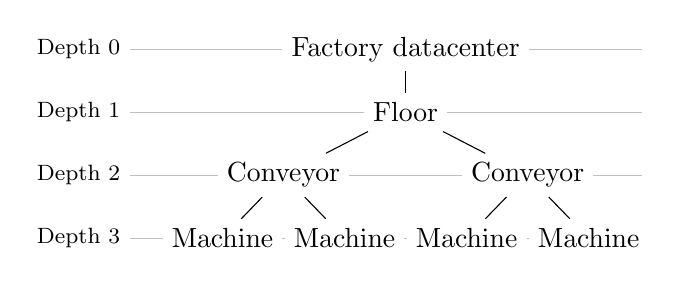
\begin{tikzpicture}[level distance=0.8cm]

	\tikzstyle{level 1}=[sibling distance=6.3cm]
	\tikzstyle{level 2}=[sibling distance=3.1cm]
	\tikzstyle{level 3}=[sibling distance=1.55cm]
	
	\node[fill=white] (d) {Factory datacenter}
%		child {node[fill=white] (f1) {Floor}
%			child { node[fill=white] (c1) {Conveyor} 
%				child { node[fill=white] (m11) {Machine} }
%				child { node[fill=white] (m12) {Machine} }	
%			}
%			child { node[fill=white] (c2) {Conveyor}
%				child { node[fill=white] (m21) {Machine} }
%				child { node[fill=white] (m22) {Machine} }
%			}
%		}
		child {node[fill=white] (f1) {Floor}
			child { node[fill=white] (c1) {Conveyor} 
				child { node[fill=white] (m11) {Machine} }
				child { node[fill=white] (m12) {Machine} }	
			}
			child { node[fill=white] (c2) {Conveyor}
				child { node[fill=white] (m21) {Machine} }
				child { node[fill=white] (m22) {Machine} }
			}
		};

\begin{pgfonlayer}{background}
	\draw[lightgray, draw] (-3.5, -0.0) node[black, left] {\footnotesize Depth 0} -- (3,-0.0);
	\draw[lightgray, draw] (-3.5, -0.8) node[black, left] {\footnotesize Depth 1} -- (3,-0.8);
	\draw[lightgray, draw] (-3.5, -1.6) node[black, left] {\footnotesize Depth 2} -- (3,-1.6);
	\draw[lightgray, draw] (-3.5, -2.4) node[black, left] {\footnotesize Depth 3} -- (3,-2.4);
\end{pgfonlayer}
	
	
\end{tikzpicture}
%\end{document}
	}
\end{figure}

\begin{table}
	\centering
	\caption{Machines hosts for distribution experiments}
	\label{tab:distrib_hosts}
	\scalebox{0.92}{
		\begin{tabular}{|c|c|c|c|c|}
			\hline
			\textbf{Virtual node}	&Datacenter	&Floor	&Conveyor		&Machine \\ \hline
			\textbf{Physical host}	&Server		&Laptop	&Raspberry Pi	&Server\\ \hline
		\end{tabular}
	}
\end{table}

To measure how distribution impacts responsiveness, four topologies were distinguished, labeled d1 to d4 and further on simply denoted d*. Each of these topologies is composed of 42 identical nodes, and processes data according to four rules, r1 to r4.
The difference between the four d* topologies is the location of sensors, as depicted in Fig. \ref{fig:dstar}. 
Sensors producing data of the type $\rho_{1}$ are directly attached to the top node in d1, while they are attached to its children in d2. 
Since $body_t(r1)=\{\rho_{1}, \rho_{4}\}$, $r1$ is applied at a maximum depth of 1 in d1, but is propagated to nodes of depth 2 in d2, hence a ``more decentralized'' execution is performed in d2 than in d1.
Rule execution depths are given in Tab. \ref{tab:factory_distrib_topologies}: in d4, all sensors are connected to leaf nodes, and the distribution is maximal.

\begin{figure}
	\centering
	\caption{d* topologies}
	\label{fig:dstar}
	\subcaption{d1}
	\scalebox{0.75}{
		\begin{forest}
[B
	[F
		[G
			[R
				[$\alpha_{4}$, edge=dotted, edge label={node[midway,right]{1}}]]
			[$\alpha_{3}$, edge=dotted, edge label={node[midway,right]{2}}]
			[R
				[$\alpha_{4}$, edge=dotted, edge label={node[midway,right]{1}}]]
		]
		[$\alpha_{2}$, edge=dotted, edge label={node[midway,right]{4}}]
		[G
			[R
				[$\alpha_{4}$, edge=dotted, edge label={node[midway,right]{1}}]]
			[$\alpha_{3}$, edge=dotted, edge label={node[midway,right]{2}}]
			[R
				[$\alpha_{4}$, edge=dotted, edge label={node[midway,right]{1}}]]
		]]
	[$\alpha_{1}$, edge=dotted, edge label={node[midway,right]{\textbf{8}}}]
	[F
		[G
			[R
				[$\alpha_{4}$, edge=dotted, edge label={node[midway,right]{1}}]]
			[$\alpha_{3}$, edge=dotted, edge label={node[midway,right]{2}}]
			[R
				[$\alpha_{4}$, edge=dotted, edge label={node[midway,right]{1}}]]]
		[$\alpha_{2}$, edge=dotted, edge label={node[midway,right]{4}}]
		[G
			[R
				[$\alpha_{4}$, edge=dotted, edge label={node[midway,right]{1}}]]
			[$\alpha_{3}$, edge=dotted, edge label={node[midway,right]{2}}]
			[R
				[$\alpha_{4}$, edge=dotted, edge label={node[midway,right]{1}}]]
	]]]
\end{forest}

	}
	
	\centering
	\subcaption{d2}
	\scalebox{0.75}{
		\begin{forest}
[B
	[F
		[G
			[R
				[$\alpha_{4}$, edge=dotted, edge label={node[midway,right]{1}}]]
			[$\alpha_{3}$, edge=dotted, edge label={node[midway,right]{2}}]
			[R
				[$\alpha_{4}$, edge=dotted, edge label={node[midway,right]{1}}]]
		]
		[$\alpha_{2}$, edge=dotted, edge label={node[midway,right]{4}}]
		[$\alpha_{1}$, edge=dotted, edge label={node[midway,right]{\textbf{4}}}]
		[G
			[R
				[$\alpha_{4}$, edge=dotted, edge label={node[midway,right]{1}}]]
			[$\alpha_{3}$, edge=dotted, edge label={node[midway,right]{2}}]
			[R
				[$\alpha_{4}$, edge=dotted, edge label={node[midway,right]{1}}]]
		]]
	[F
		[G
			[R
				[$\alpha_{4}$, edge=dotted, edge label={node[midway,right]{1}}]]
			[$\alpha_{3}$, edge=dotted, edge label={node[midway,right]{2}}]
			[R
				[$\alpha_{4}$, edge=dotted, edge label={node[midway,right]{1}}]]]
		[$\alpha_{2}$, edge=dotted, edge label={node[midway,right]{4}}]
		[$\alpha_{1}$, edge=dotted, edge label={node[midway,right]{\textbf{4}}}]
		[G
			[R
				[$\alpha_{4}$, edge=dotted, edge label={node[midway,right]{1}}]]
			[$\alpha_{3}$, edge=dotted, edge label={node[midway,right]{2}}]
			[R
				[$\alpha_{4}$, edge=dotted, edge label={node[midway,right]{1}}]]
	]]]
\end{forest}

	}
	
%	\centering
%	\subcaption{d3}
%	\scalebox{0.9}{\begin{forest}
[B
	[F
		[G
			[R
				[$\alpha_{4}$, edge=dotted, edge label={node[midway,right]{1}}]]
			[$\alpha_{3}$, edge=dotted, edge label={node[midway,right]{2}}]
			[$\alpha_{2}$, edge=dotted, edge label={node[midway,right]{\textbf{2}}}]
			[$\alpha_{1}$, edge=dotted, edge label={node[midway,right]{\textbf{2}}}]
			[R
				[$\alpha_{4}$, edge=dotted, edge label={node[midway,right]{1}}]]
		]
		[G
			[R
				[$\alpha_{4}$, edge=dotted, edge label={node[midway,right]{1}}]]
			[$\alpha_{3}$, edge=dotted, edge label={node[midway,right]{2}}]
			[$\alpha_{2}$, edge=dotted, edge label={node[midway,right]{\textbf{2}}}]
			[$\alpha_{1}$, edge=dotted, edge label={node[midway,right]{\textbf{2}}}]
			[R
				[$\alpha_{4}$, edge=dotted, edge label={node[midway,right]{1}}]]
		]]
	[F...]]
\end{forest}
}
%	
%	\centering
%	\subcaption{d4}
%	\scalebox{0.9}{\begin{forest}
[B
	[F
		[G
			[R
				[$\alpha_{4}$, edge=dotted, edge label={node[midway,right]{1}}]
				[$\alpha_{3}$, edge=dotted, edge label={node[midway,right]{\textbf{1}}}]
				[$\alpha_{2}$, edge=dotted, edge label={node[midway,right]{\textbf{1}}}]
				[$\alpha_{1}$, edge=dotted, edge label={node[midway,right]{\textbf{1}}}]]
			[R
				[$\alpha_{4}$, edge=dotted, edge label={node[midway,right]{1}}]
				[$\alpha_{3}$, edge=dotted, edge label={node[midway,right]{\textbf{1}}}]
				[$\alpha_{2}$, edge=dotted, edge label={node[midway,right]{\textbf{1}}}]
				[$\alpha_{1}$, edge=dotted, edge label={node[midway,right]{\textbf{1}}}]]
		]
		[G
			[R
				[$\alpha_{4}$, edge=dotted, edge label={node[midway,right]{1}}]
				[$\alpha_{3}$, edge=dotted, edge label={node[midway,right]{\textbf{1}}}]
				[$\alpha_{2}$, edge=dotted, edge label={node[midway,right]{\textbf{1}}}]
				[$\alpha_{1}$, edge=dotted, edge label={node[midway,right]{\textbf{1}}}]]
			[R...]
		]]
	[F...]]
\end{forest}
}
\end{figure}

To assess the impact of distribution, the same sensors are deployed from topology d0 to d4, but they are not situated at the same level, enabling the control of the level at which rules are processed.
Sensors are situated in d* topologies so that the rules are processed at the depths depicted in Tab. \ref{tab:factory_distrib_topologies}.
The simulation topology is composed of 42 nodes in total (including sensors), hosted on the physical machines as detailed on Tab. \ref{tab:distrib_hosts}.
Fig. \ref{fig:factory_distribution_single-host} displays results for single-host approaches, and Fig. \ref{fig:factory_distribution_multi-host} for multi-host approaches, both showing centralized and distributed reasoning. 

\begin{table}
	\centering
	\caption{Depth of rule processing for d*}
	\label{tab:factory_distrib_topologies}
	\begin{tabular}{|c|c|c|c|c|c|c|c|}
		\hline
		&\textbf{R1}&\textbf{R2}&\textbf{R3}&\textbf{R4}&\textbf{R5}&\textbf{R6}&\textbf{R7}\\ \hline
		\textbf{d0}& 0& 0& 0& 0& 0& 0& 0\\ \hline
		\textbf{d1}& 0& 1& 0& 1& 1& 0& 0\\ \hline
		\textbf{d2}& 1& 1& 0& 1& 1& 0& 0\\ \hline
		\textbf{d3}& 1& 1& 0& 3& 3& 1& 3\\ \hline
		\textbf{d4}& 3& 2& 2& 3& 3& 2& 3\\ \hline
	\end{tabular}
\end{table}

\subsubsection{Results}

\begin{figure*}
	\Centering
	\caption{\Centering Distribution experiments, single-host execution}
	\label{fig:factory_distribution_single-host}
	\begin{minipage}{0.395\textwidth}
		\Centering
		\subcaption{\Centering Centralized reasoning}
		\label{fig:factory_distribution_raw_syn}
		\scalebox{0.8}{
			%% Creator: Matplotlib, PGF backend
%%
%% To include the figure in your LaTeX document, write
%%   \input{<filename>.pgf}
%%
%% Make sure the required packages are loaded in your preamble
%%   \usepackage{pgf}
%%
%% Figures using additional raster images can only be included by \input if
%% they are in the same directory as the main LaTeX file. For loading figures
%% from other directories you can use the `import` package
%%   \usepackage{import}
%% and then include the figures with
%%   \import{<path to file>}{<filename>.pgf}
%%
%% Matplotlib used the following preamble
%%   \usepackage{fontspec}
%%   \setsansfont{DejaVu Sans}
%%   \setmonofont{DejaVu Sans Mono}
%%
\begingroup%
\makeatletter%
\begin{pgfpicture}%
\pgfpathrectangle{\pgfpointorigin}{\pgfqpoint{3.000000in}{2.000000in}}%
\pgfusepath{use as bounding box, clip}%
\begin{pgfscope}%
\pgfsetbuttcap%
\pgfsetmiterjoin%
\definecolor{currentfill}{rgb}{1.000000,1.000000,1.000000}%
\pgfsetfillcolor{currentfill}%
\pgfsetlinewidth{0.000000pt}%
\definecolor{currentstroke}{rgb}{1.000000,1.000000,1.000000}%
\pgfsetstrokecolor{currentstroke}%
\pgfsetdash{}{0pt}%
\pgfpathmoveto{\pgfqpoint{0.000000in}{0.000000in}}%
\pgfpathlineto{\pgfqpoint{3.000000in}{0.000000in}}%
\pgfpathlineto{\pgfqpoint{3.000000in}{2.000000in}}%
\pgfpathlineto{\pgfqpoint{0.000000in}{2.000000in}}%
\pgfpathclose%
\pgfusepath{fill}%
\end{pgfscope}%
\begin{pgfscope}%
\pgfsetbuttcap%
\pgfsetmiterjoin%
\definecolor{currentfill}{rgb}{1.000000,1.000000,1.000000}%
\pgfsetfillcolor{currentfill}%
\pgfsetlinewidth{0.000000pt}%
\definecolor{currentstroke}{rgb}{0.000000,0.000000,0.000000}%
\pgfsetstrokecolor{currentstroke}%
\pgfsetstrokeopacity{0.000000}%
\pgfsetdash{}{0pt}%
\pgfpathmoveto{\pgfqpoint{0.450000in}{0.400000in}}%
\pgfpathlineto{\pgfqpoint{2.970000in}{0.400000in}}%
\pgfpathlineto{\pgfqpoint{2.970000in}{1.980000in}}%
\pgfpathlineto{\pgfqpoint{0.450000in}{1.980000in}}%
\pgfpathclose%
\pgfusepath{fill}%
\end{pgfscope}%
\begin{pgfscope}%
\pgfsetbuttcap%
\pgfsetroundjoin%
\definecolor{currentfill}{rgb}{0.000000,0.000000,0.000000}%
\pgfsetfillcolor{currentfill}%
\pgfsetlinewidth{0.803000pt}%
\definecolor{currentstroke}{rgb}{0.000000,0.000000,0.000000}%
\pgfsetstrokecolor{currentstroke}%
\pgfsetdash{}{0pt}%
\pgfsys@defobject{currentmarker}{\pgfqpoint{0.000000in}{-0.048611in}}{\pgfqpoint{0.000000in}{0.000000in}}{%
\pgfpathmoveto{\pgfqpoint{0.000000in}{0.000000in}}%
\pgfpathlineto{\pgfqpoint{0.000000in}{-0.048611in}}%
\pgfusepath{stroke,fill}%
}%
\begin{pgfscope}%
\pgfsys@transformshift{0.576000in}{0.400000in}%
\pgfsys@useobject{currentmarker}{}%
\end{pgfscope}%
\end{pgfscope}%
\begin{pgfscope}%
\pgftext[x=0.483361in,y=0.206389in,left,base]{\rmfamily\fontsize{10.000000}{12.000000}\selectfont d0}%
\end{pgfscope}%
\begin{pgfscope}%
\pgftext[x=0.498639in,y=0.063778in,left,base]{\rmfamily\fontsize{10.000000}{12.000000}\selectfont cir}%
\end{pgfscope}%
\begin{pgfscope}%
\pgfsetbuttcap%
\pgfsetroundjoin%
\definecolor{currentfill}{rgb}{0.000000,0.000000,0.000000}%
\pgfsetfillcolor{currentfill}%
\pgfsetlinewidth{0.803000pt}%
\definecolor{currentstroke}{rgb}{0.000000,0.000000,0.000000}%
\pgfsetstrokecolor{currentstroke}%
\pgfsetdash{}{0pt}%
\pgfsys@defobject{currentmarker}{\pgfqpoint{0.000000in}{-0.048611in}}{\pgfqpoint{0.000000in}{0.000000in}}{%
\pgfpathmoveto{\pgfqpoint{0.000000in}{0.000000in}}%
\pgfpathlineto{\pgfqpoint{0.000000in}{-0.048611in}}%
\pgfusepath{stroke,fill}%
}%
\begin{pgfscope}%
\pgfsys@transformshift{0.828000in}{0.400000in}%
\pgfsys@useobject{currentmarker}{}%
\end{pgfscope}%
\end{pgfscope}%
\begin{pgfscope}%
\pgftext[x=0.735361in,y=0.206389in,left,base]{\rmfamily\fontsize{10.000000}{12.000000}\selectfont d1}%
\end{pgfscope}%
\begin{pgfscope}%
\pgftext[x=0.750639in,y=0.063778in,left,base]{\rmfamily\fontsize{10.000000}{12.000000}\selectfont cir}%
\end{pgfscope}%
\begin{pgfscope}%
\pgfsetbuttcap%
\pgfsetroundjoin%
\definecolor{currentfill}{rgb}{0.000000,0.000000,0.000000}%
\pgfsetfillcolor{currentfill}%
\pgfsetlinewidth{0.803000pt}%
\definecolor{currentstroke}{rgb}{0.000000,0.000000,0.000000}%
\pgfsetstrokecolor{currentstroke}%
\pgfsetdash{}{0pt}%
\pgfsys@defobject{currentmarker}{\pgfqpoint{0.000000in}{-0.048611in}}{\pgfqpoint{0.000000in}{0.000000in}}{%
\pgfpathmoveto{\pgfqpoint{0.000000in}{0.000000in}}%
\pgfpathlineto{\pgfqpoint{0.000000in}{-0.048611in}}%
\pgfusepath{stroke,fill}%
}%
\begin{pgfscope}%
\pgfsys@transformshift{1.080000in}{0.400000in}%
\pgfsys@useobject{currentmarker}{}%
\end{pgfscope}%
\end{pgfscope}%
\begin{pgfscope}%
\pgftext[x=0.987361in,y=0.206389in,left,base]{\rmfamily\fontsize{10.000000}{12.000000}\selectfont d2}%
\end{pgfscope}%
\begin{pgfscope}%
\pgftext[x=1.002639in,y=0.063778in,left,base]{\rmfamily\fontsize{10.000000}{12.000000}\selectfont cir}%
\end{pgfscope}%
\begin{pgfscope}%
\pgfsetbuttcap%
\pgfsetroundjoin%
\definecolor{currentfill}{rgb}{0.000000,0.000000,0.000000}%
\pgfsetfillcolor{currentfill}%
\pgfsetlinewidth{0.803000pt}%
\definecolor{currentstroke}{rgb}{0.000000,0.000000,0.000000}%
\pgfsetstrokecolor{currentstroke}%
\pgfsetdash{}{0pt}%
\pgfsys@defobject{currentmarker}{\pgfqpoint{0.000000in}{-0.048611in}}{\pgfqpoint{0.000000in}{0.000000in}}{%
\pgfpathmoveto{\pgfqpoint{0.000000in}{0.000000in}}%
\pgfpathlineto{\pgfqpoint{0.000000in}{-0.048611in}}%
\pgfusepath{stroke,fill}%
}%
\begin{pgfscope}%
\pgfsys@transformshift{1.332000in}{0.400000in}%
\pgfsys@useobject{currentmarker}{}%
\end{pgfscope}%
\end{pgfscope}%
\begin{pgfscope}%
\pgftext[x=1.239361in,y=0.206389in,left,base]{\rmfamily\fontsize{10.000000}{12.000000}\selectfont d3}%
\end{pgfscope}%
\begin{pgfscope}%
\pgftext[x=1.254639in,y=0.063778in,left,base]{\rmfamily\fontsize{10.000000}{12.000000}\selectfont cir}%
\end{pgfscope}%
\begin{pgfscope}%
\pgfsetbuttcap%
\pgfsetroundjoin%
\definecolor{currentfill}{rgb}{0.000000,0.000000,0.000000}%
\pgfsetfillcolor{currentfill}%
\pgfsetlinewidth{0.803000pt}%
\definecolor{currentstroke}{rgb}{0.000000,0.000000,0.000000}%
\pgfsetstrokecolor{currentstroke}%
\pgfsetdash{}{0pt}%
\pgfsys@defobject{currentmarker}{\pgfqpoint{0.000000in}{-0.048611in}}{\pgfqpoint{0.000000in}{0.000000in}}{%
\pgfpathmoveto{\pgfqpoint{0.000000in}{0.000000in}}%
\pgfpathlineto{\pgfqpoint{0.000000in}{-0.048611in}}%
\pgfusepath{stroke,fill}%
}%
\begin{pgfscope}%
\pgfsys@transformshift{1.584000in}{0.400000in}%
\pgfsys@useobject{currentmarker}{}%
\end{pgfscope}%
\end{pgfscope}%
\begin{pgfscope}%
\pgftext[x=1.491361in,y=0.206389in,left,base]{\rmfamily\fontsize{10.000000}{12.000000}\selectfont d4}%
\end{pgfscope}%
\begin{pgfscope}%
\pgftext[x=1.506639in,y=0.063778in,left,base]{\rmfamily\fontsize{10.000000}{12.000000}\selectfont cir}%
\end{pgfscope}%
\begin{pgfscope}%
\pgfsetbuttcap%
\pgfsetroundjoin%
\definecolor{currentfill}{rgb}{0.000000,0.000000,0.000000}%
\pgfsetfillcolor{currentfill}%
\pgfsetlinewidth{0.803000pt}%
\definecolor{currentstroke}{rgb}{0.000000,0.000000,0.000000}%
\pgfsetstrokecolor{currentstroke}%
\pgfsetdash{}{0pt}%
\pgfsys@defobject{currentmarker}{\pgfqpoint{0.000000in}{-0.048611in}}{\pgfqpoint{0.000000in}{0.000000in}}{%
\pgfpathmoveto{\pgfqpoint{0.000000in}{0.000000in}}%
\pgfpathlineto{\pgfqpoint{0.000000in}{-0.048611in}}%
\pgfusepath{stroke,fill}%
}%
\begin{pgfscope}%
\pgfsys@transformshift{1.836000in}{0.400000in}%
\pgfsys@useobject{currentmarker}{}%
\end{pgfscope}%
\end{pgfscope}%
\begin{pgfscope}%
\pgftext[x=1.743361in,y=0.206389in,left,base]{\rmfamily\fontsize{10.000000}{12.000000}\selectfont d0}%
\end{pgfscope}%
\begin{pgfscope}%
\pgftext[x=1.739333in,y=0.063778in,left,base]{\rmfamily\fontsize{10.000000}{12.000000}\selectfont cdr}%
\end{pgfscope}%
\begin{pgfscope}%
\pgfsetbuttcap%
\pgfsetroundjoin%
\definecolor{currentfill}{rgb}{0.000000,0.000000,0.000000}%
\pgfsetfillcolor{currentfill}%
\pgfsetlinewidth{0.803000pt}%
\definecolor{currentstroke}{rgb}{0.000000,0.000000,0.000000}%
\pgfsetstrokecolor{currentstroke}%
\pgfsetdash{}{0pt}%
\pgfsys@defobject{currentmarker}{\pgfqpoint{0.000000in}{-0.048611in}}{\pgfqpoint{0.000000in}{0.000000in}}{%
\pgfpathmoveto{\pgfqpoint{0.000000in}{0.000000in}}%
\pgfpathlineto{\pgfqpoint{0.000000in}{-0.048611in}}%
\pgfusepath{stroke,fill}%
}%
\begin{pgfscope}%
\pgfsys@transformshift{2.088000in}{0.400000in}%
\pgfsys@useobject{currentmarker}{}%
\end{pgfscope}%
\end{pgfscope}%
\begin{pgfscope}%
\pgftext[x=1.995361in,y=0.206389in,left,base]{\rmfamily\fontsize{10.000000}{12.000000}\selectfont d1}%
\end{pgfscope}%
\begin{pgfscope}%
\pgftext[x=1.991333in,y=0.063778in,left,base]{\rmfamily\fontsize{10.000000}{12.000000}\selectfont cdr}%
\end{pgfscope}%
\begin{pgfscope}%
\pgfsetbuttcap%
\pgfsetroundjoin%
\definecolor{currentfill}{rgb}{0.000000,0.000000,0.000000}%
\pgfsetfillcolor{currentfill}%
\pgfsetlinewidth{0.803000pt}%
\definecolor{currentstroke}{rgb}{0.000000,0.000000,0.000000}%
\pgfsetstrokecolor{currentstroke}%
\pgfsetdash{}{0pt}%
\pgfsys@defobject{currentmarker}{\pgfqpoint{0.000000in}{-0.048611in}}{\pgfqpoint{0.000000in}{0.000000in}}{%
\pgfpathmoveto{\pgfqpoint{0.000000in}{0.000000in}}%
\pgfpathlineto{\pgfqpoint{0.000000in}{-0.048611in}}%
\pgfusepath{stroke,fill}%
}%
\begin{pgfscope}%
\pgfsys@transformshift{2.340000in}{0.400000in}%
\pgfsys@useobject{currentmarker}{}%
\end{pgfscope}%
\end{pgfscope}%
\begin{pgfscope}%
\pgftext[x=2.247361in,y=0.206389in,left,base]{\rmfamily\fontsize{10.000000}{12.000000}\selectfont d2}%
\end{pgfscope}%
\begin{pgfscope}%
\pgftext[x=2.243333in,y=0.063778in,left,base]{\rmfamily\fontsize{10.000000}{12.000000}\selectfont cdr}%
\end{pgfscope}%
\begin{pgfscope}%
\pgfsetbuttcap%
\pgfsetroundjoin%
\definecolor{currentfill}{rgb}{0.000000,0.000000,0.000000}%
\pgfsetfillcolor{currentfill}%
\pgfsetlinewidth{0.803000pt}%
\definecolor{currentstroke}{rgb}{0.000000,0.000000,0.000000}%
\pgfsetstrokecolor{currentstroke}%
\pgfsetdash{}{0pt}%
\pgfsys@defobject{currentmarker}{\pgfqpoint{0.000000in}{-0.048611in}}{\pgfqpoint{0.000000in}{0.000000in}}{%
\pgfpathmoveto{\pgfqpoint{0.000000in}{0.000000in}}%
\pgfpathlineto{\pgfqpoint{0.000000in}{-0.048611in}}%
\pgfusepath{stroke,fill}%
}%
\begin{pgfscope}%
\pgfsys@transformshift{2.592000in}{0.400000in}%
\pgfsys@useobject{currentmarker}{}%
\end{pgfscope}%
\end{pgfscope}%
\begin{pgfscope}%
\pgftext[x=2.499361in,y=0.206389in,left,base]{\rmfamily\fontsize{10.000000}{12.000000}\selectfont d3}%
\end{pgfscope}%
\begin{pgfscope}%
\pgftext[x=2.495333in,y=0.063778in,left,base]{\rmfamily\fontsize{10.000000}{12.000000}\selectfont cdr}%
\end{pgfscope}%
\begin{pgfscope}%
\pgfsetbuttcap%
\pgfsetroundjoin%
\definecolor{currentfill}{rgb}{0.000000,0.000000,0.000000}%
\pgfsetfillcolor{currentfill}%
\pgfsetlinewidth{0.803000pt}%
\definecolor{currentstroke}{rgb}{0.000000,0.000000,0.000000}%
\pgfsetstrokecolor{currentstroke}%
\pgfsetdash{}{0pt}%
\pgfsys@defobject{currentmarker}{\pgfqpoint{0.000000in}{-0.048611in}}{\pgfqpoint{0.000000in}{0.000000in}}{%
\pgfpathmoveto{\pgfqpoint{0.000000in}{0.000000in}}%
\pgfpathlineto{\pgfqpoint{0.000000in}{-0.048611in}}%
\pgfusepath{stroke,fill}%
}%
\begin{pgfscope}%
\pgfsys@transformshift{2.844000in}{0.400000in}%
\pgfsys@useobject{currentmarker}{}%
\end{pgfscope}%
\end{pgfscope}%
\begin{pgfscope}%
\pgftext[x=2.751361in,y=0.206389in,left,base]{\rmfamily\fontsize{10.000000}{12.000000}\selectfont d4}%
\end{pgfscope}%
\begin{pgfscope}%
\pgftext[x=2.747333in,y=0.063778in,left,base]{\rmfamily\fontsize{10.000000}{12.000000}\selectfont cdr}%
\end{pgfscope}%
\begin{pgfscope}%
\pgfpathrectangle{\pgfqpoint{0.450000in}{0.400000in}}{\pgfqpoint{2.520000in}{1.580000in}} %
\pgfusepath{clip}%
\pgfsetbuttcap%
\pgfsetroundjoin%
\pgfsetlinewidth{0.803000pt}%
\definecolor{currentstroke}{rgb}{0.690196,0.690196,0.690196}%
\pgfsetstrokecolor{currentstroke}%
\pgfsetdash{{2.960000pt}{1.280000pt}}{0.000000pt}%
\pgfpathmoveto{\pgfqpoint{0.450000in}{0.454805in}}%
\pgfpathlineto{\pgfqpoint{2.970000in}{0.454805in}}%
\pgfusepath{stroke}%
\end{pgfscope}%
\begin{pgfscope}%
\pgfsetbuttcap%
\pgfsetroundjoin%
\definecolor{currentfill}{rgb}{0.000000,0.000000,0.000000}%
\pgfsetfillcolor{currentfill}%
\pgfsetlinewidth{0.803000pt}%
\definecolor{currentstroke}{rgb}{0.000000,0.000000,0.000000}%
\pgfsetstrokecolor{currentstroke}%
\pgfsetdash{}{0pt}%
\pgfsys@defobject{currentmarker}{\pgfqpoint{-0.048611in}{0.000000in}}{\pgfqpoint{0.000000in}{0.000000in}}{%
\pgfpathmoveto{\pgfqpoint{0.000000in}{0.000000in}}%
\pgfpathlineto{\pgfqpoint{-0.048611in}{0.000000in}}%
\pgfusepath{stroke,fill}%
}%
\begin{pgfscope}%
\pgfsys@transformshift{0.450000in}{0.454805in}%
\pgfsys@useobject{currentmarker}{}%
\end{pgfscope}%
\end{pgfscope}%
\begin{pgfscope}%
\pgftext[x=0.283333in,y=0.406611in,left,base]{\rmfamily\fontsize{10.000000}{12.000000}\selectfont \(\displaystyle 0\)}%
\end{pgfscope}%
\begin{pgfscope}%
\pgfpathrectangle{\pgfqpoint{0.450000in}{0.400000in}}{\pgfqpoint{2.520000in}{1.580000in}} %
\pgfusepath{clip}%
\pgfsetbuttcap%
\pgfsetroundjoin%
\pgfsetlinewidth{0.803000pt}%
\definecolor{currentstroke}{rgb}{0.690196,0.690196,0.690196}%
\pgfsetstrokecolor{currentstroke}%
\pgfsetdash{{2.960000pt}{1.280000pt}}{0.000000pt}%
\pgfpathmoveto{\pgfqpoint{0.450000in}{0.606705in}}%
\pgfpathlineto{\pgfqpoint{2.970000in}{0.606705in}}%
\pgfusepath{stroke}%
\end{pgfscope}%
\begin{pgfscope}%
\pgfsetbuttcap%
\pgfsetroundjoin%
\definecolor{currentfill}{rgb}{0.000000,0.000000,0.000000}%
\pgfsetfillcolor{currentfill}%
\pgfsetlinewidth{0.803000pt}%
\definecolor{currentstroke}{rgb}{0.000000,0.000000,0.000000}%
\pgfsetstrokecolor{currentstroke}%
\pgfsetdash{}{0pt}%
\pgfsys@defobject{currentmarker}{\pgfqpoint{-0.048611in}{0.000000in}}{\pgfqpoint{0.000000in}{0.000000in}}{%
\pgfpathmoveto{\pgfqpoint{0.000000in}{0.000000in}}%
\pgfpathlineto{\pgfqpoint{-0.048611in}{0.000000in}}%
\pgfusepath{stroke,fill}%
}%
\begin{pgfscope}%
\pgfsys@transformshift{0.450000in}{0.606705in}%
\pgfsys@useobject{currentmarker}{}%
\end{pgfscope}%
\end{pgfscope}%
\begin{pgfscope}%
\pgftext[x=0.283333in,y=0.558511in,left,base]{\rmfamily\fontsize{10.000000}{12.000000}\selectfont \(\displaystyle 1\)}%
\end{pgfscope}%
\begin{pgfscope}%
\pgfpathrectangle{\pgfqpoint{0.450000in}{0.400000in}}{\pgfqpoint{2.520000in}{1.580000in}} %
\pgfusepath{clip}%
\pgfsetbuttcap%
\pgfsetroundjoin%
\pgfsetlinewidth{0.803000pt}%
\definecolor{currentstroke}{rgb}{0.690196,0.690196,0.690196}%
\pgfsetstrokecolor{currentstroke}%
\pgfsetdash{{2.960000pt}{1.280000pt}}{0.000000pt}%
\pgfpathmoveto{\pgfqpoint{0.450000in}{0.758605in}}%
\pgfpathlineto{\pgfqpoint{2.970000in}{0.758605in}}%
\pgfusepath{stroke}%
\end{pgfscope}%
\begin{pgfscope}%
\pgfsetbuttcap%
\pgfsetroundjoin%
\definecolor{currentfill}{rgb}{0.000000,0.000000,0.000000}%
\pgfsetfillcolor{currentfill}%
\pgfsetlinewidth{0.803000pt}%
\definecolor{currentstroke}{rgb}{0.000000,0.000000,0.000000}%
\pgfsetstrokecolor{currentstroke}%
\pgfsetdash{}{0pt}%
\pgfsys@defobject{currentmarker}{\pgfqpoint{-0.048611in}{0.000000in}}{\pgfqpoint{0.000000in}{0.000000in}}{%
\pgfpathmoveto{\pgfqpoint{0.000000in}{0.000000in}}%
\pgfpathlineto{\pgfqpoint{-0.048611in}{0.000000in}}%
\pgfusepath{stroke,fill}%
}%
\begin{pgfscope}%
\pgfsys@transformshift{0.450000in}{0.758605in}%
\pgfsys@useobject{currentmarker}{}%
\end{pgfscope}%
\end{pgfscope}%
\begin{pgfscope}%
\pgftext[x=0.283333in,y=0.710410in,left,base]{\rmfamily\fontsize{10.000000}{12.000000}\selectfont \(\displaystyle 2\)}%
\end{pgfscope}%
\begin{pgfscope}%
\pgfpathrectangle{\pgfqpoint{0.450000in}{0.400000in}}{\pgfqpoint{2.520000in}{1.580000in}} %
\pgfusepath{clip}%
\pgfsetbuttcap%
\pgfsetroundjoin%
\pgfsetlinewidth{0.803000pt}%
\definecolor{currentstroke}{rgb}{0.690196,0.690196,0.690196}%
\pgfsetstrokecolor{currentstroke}%
\pgfsetdash{{2.960000pt}{1.280000pt}}{0.000000pt}%
\pgfpathmoveto{\pgfqpoint{0.450000in}{0.910505in}}%
\pgfpathlineto{\pgfqpoint{2.970000in}{0.910505in}}%
\pgfusepath{stroke}%
\end{pgfscope}%
\begin{pgfscope}%
\pgfsetbuttcap%
\pgfsetroundjoin%
\definecolor{currentfill}{rgb}{0.000000,0.000000,0.000000}%
\pgfsetfillcolor{currentfill}%
\pgfsetlinewidth{0.803000pt}%
\definecolor{currentstroke}{rgb}{0.000000,0.000000,0.000000}%
\pgfsetstrokecolor{currentstroke}%
\pgfsetdash{}{0pt}%
\pgfsys@defobject{currentmarker}{\pgfqpoint{-0.048611in}{0.000000in}}{\pgfqpoint{0.000000in}{0.000000in}}{%
\pgfpathmoveto{\pgfqpoint{0.000000in}{0.000000in}}%
\pgfpathlineto{\pgfqpoint{-0.048611in}{0.000000in}}%
\pgfusepath{stroke,fill}%
}%
\begin{pgfscope}%
\pgfsys@transformshift{0.450000in}{0.910505in}%
\pgfsys@useobject{currentmarker}{}%
\end{pgfscope}%
\end{pgfscope}%
\begin{pgfscope}%
\pgftext[x=0.283333in,y=0.862310in,left,base]{\rmfamily\fontsize{10.000000}{12.000000}\selectfont \(\displaystyle 3\)}%
\end{pgfscope}%
\begin{pgfscope}%
\pgfpathrectangle{\pgfqpoint{0.450000in}{0.400000in}}{\pgfqpoint{2.520000in}{1.580000in}} %
\pgfusepath{clip}%
\pgfsetbuttcap%
\pgfsetroundjoin%
\pgfsetlinewidth{0.803000pt}%
\definecolor{currentstroke}{rgb}{0.690196,0.690196,0.690196}%
\pgfsetstrokecolor{currentstroke}%
\pgfsetdash{{2.960000pt}{1.280000pt}}{0.000000pt}%
\pgfpathmoveto{\pgfqpoint{0.450000in}{1.062404in}}%
\pgfpathlineto{\pgfqpoint{2.970000in}{1.062404in}}%
\pgfusepath{stroke}%
\end{pgfscope}%
\begin{pgfscope}%
\pgfsetbuttcap%
\pgfsetroundjoin%
\definecolor{currentfill}{rgb}{0.000000,0.000000,0.000000}%
\pgfsetfillcolor{currentfill}%
\pgfsetlinewidth{0.803000pt}%
\definecolor{currentstroke}{rgb}{0.000000,0.000000,0.000000}%
\pgfsetstrokecolor{currentstroke}%
\pgfsetdash{}{0pt}%
\pgfsys@defobject{currentmarker}{\pgfqpoint{-0.048611in}{0.000000in}}{\pgfqpoint{0.000000in}{0.000000in}}{%
\pgfpathmoveto{\pgfqpoint{0.000000in}{0.000000in}}%
\pgfpathlineto{\pgfqpoint{-0.048611in}{0.000000in}}%
\pgfusepath{stroke,fill}%
}%
\begin{pgfscope}%
\pgfsys@transformshift{0.450000in}{1.062404in}%
\pgfsys@useobject{currentmarker}{}%
\end{pgfscope}%
\end{pgfscope}%
\begin{pgfscope}%
\pgftext[x=0.283333in,y=1.014210in,left,base]{\rmfamily\fontsize{10.000000}{12.000000}\selectfont \(\displaystyle 4\)}%
\end{pgfscope}%
\begin{pgfscope}%
\pgfpathrectangle{\pgfqpoint{0.450000in}{0.400000in}}{\pgfqpoint{2.520000in}{1.580000in}} %
\pgfusepath{clip}%
\pgfsetbuttcap%
\pgfsetroundjoin%
\pgfsetlinewidth{0.803000pt}%
\definecolor{currentstroke}{rgb}{0.690196,0.690196,0.690196}%
\pgfsetstrokecolor{currentstroke}%
\pgfsetdash{{2.960000pt}{1.280000pt}}{0.000000pt}%
\pgfpathmoveto{\pgfqpoint{0.450000in}{1.214304in}}%
\pgfpathlineto{\pgfqpoint{2.970000in}{1.214304in}}%
\pgfusepath{stroke}%
\end{pgfscope}%
\begin{pgfscope}%
\pgfsetbuttcap%
\pgfsetroundjoin%
\definecolor{currentfill}{rgb}{0.000000,0.000000,0.000000}%
\pgfsetfillcolor{currentfill}%
\pgfsetlinewidth{0.803000pt}%
\definecolor{currentstroke}{rgb}{0.000000,0.000000,0.000000}%
\pgfsetstrokecolor{currentstroke}%
\pgfsetdash{}{0pt}%
\pgfsys@defobject{currentmarker}{\pgfqpoint{-0.048611in}{0.000000in}}{\pgfqpoint{0.000000in}{0.000000in}}{%
\pgfpathmoveto{\pgfqpoint{0.000000in}{0.000000in}}%
\pgfpathlineto{\pgfqpoint{-0.048611in}{0.000000in}}%
\pgfusepath{stroke,fill}%
}%
\begin{pgfscope}%
\pgfsys@transformshift{0.450000in}{1.214304in}%
\pgfsys@useobject{currentmarker}{}%
\end{pgfscope}%
\end{pgfscope}%
\begin{pgfscope}%
\pgftext[x=0.283333in,y=1.166110in,left,base]{\rmfamily\fontsize{10.000000}{12.000000}\selectfont \(\displaystyle 5\)}%
\end{pgfscope}%
\begin{pgfscope}%
\pgfpathrectangle{\pgfqpoint{0.450000in}{0.400000in}}{\pgfqpoint{2.520000in}{1.580000in}} %
\pgfusepath{clip}%
\pgfsetbuttcap%
\pgfsetroundjoin%
\pgfsetlinewidth{0.803000pt}%
\definecolor{currentstroke}{rgb}{0.690196,0.690196,0.690196}%
\pgfsetstrokecolor{currentstroke}%
\pgfsetdash{{2.960000pt}{1.280000pt}}{0.000000pt}%
\pgfpathmoveto{\pgfqpoint{0.450000in}{1.366204in}}%
\pgfpathlineto{\pgfqpoint{2.970000in}{1.366204in}}%
\pgfusepath{stroke}%
\end{pgfscope}%
\begin{pgfscope}%
\pgfsetbuttcap%
\pgfsetroundjoin%
\definecolor{currentfill}{rgb}{0.000000,0.000000,0.000000}%
\pgfsetfillcolor{currentfill}%
\pgfsetlinewidth{0.803000pt}%
\definecolor{currentstroke}{rgb}{0.000000,0.000000,0.000000}%
\pgfsetstrokecolor{currentstroke}%
\pgfsetdash{}{0pt}%
\pgfsys@defobject{currentmarker}{\pgfqpoint{-0.048611in}{0.000000in}}{\pgfqpoint{0.000000in}{0.000000in}}{%
\pgfpathmoveto{\pgfqpoint{0.000000in}{0.000000in}}%
\pgfpathlineto{\pgfqpoint{-0.048611in}{0.000000in}}%
\pgfusepath{stroke,fill}%
}%
\begin{pgfscope}%
\pgfsys@transformshift{0.450000in}{1.366204in}%
\pgfsys@useobject{currentmarker}{}%
\end{pgfscope}%
\end{pgfscope}%
\begin{pgfscope}%
\pgftext[x=0.283333in,y=1.318009in,left,base]{\rmfamily\fontsize{10.000000}{12.000000}\selectfont \(\displaystyle 6\)}%
\end{pgfscope}%
\begin{pgfscope}%
\pgfpathrectangle{\pgfqpoint{0.450000in}{0.400000in}}{\pgfqpoint{2.520000in}{1.580000in}} %
\pgfusepath{clip}%
\pgfsetbuttcap%
\pgfsetroundjoin%
\pgfsetlinewidth{0.803000pt}%
\definecolor{currentstroke}{rgb}{0.690196,0.690196,0.690196}%
\pgfsetstrokecolor{currentstroke}%
\pgfsetdash{{2.960000pt}{1.280000pt}}{0.000000pt}%
\pgfpathmoveto{\pgfqpoint{0.450000in}{1.518103in}}%
\pgfpathlineto{\pgfqpoint{2.970000in}{1.518103in}}%
\pgfusepath{stroke}%
\end{pgfscope}%
\begin{pgfscope}%
\pgfsetbuttcap%
\pgfsetroundjoin%
\definecolor{currentfill}{rgb}{0.000000,0.000000,0.000000}%
\pgfsetfillcolor{currentfill}%
\pgfsetlinewidth{0.803000pt}%
\definecolor{currentstroke}{rgb}{0.000000,0.000000,0.000000}%
\pgfsetstrokecolor{currentstroke}%
\pgfsetdash{}{0pt}%
\pgfsys@defobject{currentmarker}{\pgfqpoint{-0.048611in}{0.000000in}}{\pgfqpoint{0.000000in}{0.000000in}}{%
\pgfpathmoveto{\pgfqpoint{0.000000in}{0.000000in}}%
\pgfpathlineto{\pgfqpoint{-0.048611in}{0.000000in}}%
\pgfusepath{stroke,fill}%
}%
\begin{pgfscope}%
\pgfsys@transformshift{0.450000in}{1.518103in}%
\pgfsys@useobject{currentmarker}{}%
\end{pgfscope}%
\end{pgfscope}%
\begin{pgfscope}%
\pgftext[x=0.283333in,y=1.469909in,left,base]{\rmfamily\fontsize{10.000000}{12.000000}\selectfont \(\displaystyle 7\)}%
\end{pgfscope}%
\begin{pgfscope}%
\pgfpathrectangle{\pgfqpoint{0.450000in}{0.400000in}}{\pgfqpoint{2.520000in}{1.580000in}} %
\pgfusepath{clip}%
\pgfsetbuttcap%
\pgfsetroundjoin%
\pgfsetlinewidth{0.803000pt}%
\definecolor{currentstroke}{rgb}{0.690196,0.690196,0.690196}%
\pgfsetstrokecolor{currentstroke}%
\pgfsetdash{{2.960000pt}{1.280000pt}}{0.000000pt}%
\pgfpathmoveto{\pgfqpoint{0.450000in}{1.670003in}}%
\pgfpathlineto{\pgfqpoint{2.970000in}{1.670003in}}%
\pgfusepath{stroke}%
\end{pgfscope}%
\begin{pgfscope}%
\pgfsetbuttcap%
\pgfsetroundjoin%
\definecolor{currentfill}{rgb}{0.000000,0.000000,0.000000}%
\pgfsetfillcolor{currentfill}%
\pgfsetlinewidth{0.803000pt}%
\definecolor{currentstroke}{rgb}{0.000000,0.000000,0.000000}%
\pgfsetstrokecolor{currentstroke}%
\pgfsetdash{}{0pt}%
\pgfsys@defobject{currentmarker}{\pgfqpoint{-0.048611in}{0.000000in}}{\pgfqpoint{0.000000in}{0.000000in}}{%
\pgfpathmoveto{\pgfqpoint{0.000000in}{0.000000in}}%
\pgfpathlineto{\pgfqpoint{-0.048611in}{0.000000in}}%
\pgfusepath{stroke,fill}%
}%
\begin{pgfscope}%
\pgfsys@transformshift{0.450000in}{1.670003in}%
\pgfsys@useobject{currentmarker}{}%
\end{pgfscope}%
\end{pgfscope}%
\begin{pgfscope}%
\pgftext[x=0.283333in,y=1.621809in,left,base]{\rmfamily\fontsize{10.000000}{12.000000}\selectfont \(\displaystyle 8\)}%
\end{pgfscope}%
\begin{pgfscope}%
\pgfpathrectangle{\pgfqpoint{0.450000in}{0.400000in}}{\pgfqpoint{2.520000in}{1.580000in}} %
\pgfusepath{clip}%
\pgfsetbuttcap%
\pgfsetroundjoin%
\pgfsetlinewidth{0.803000pt}%
\definecolor{currentstroke}{rgb}{0.690196,0.690196,0.690196}%
\pgfsetstrokecolor{currentstroke}%
\pgfsetdash{{2.960000pt}{1.280000pt}}{0.000000pt}%
\pgfpathmoveto{\pgfqpoint{0.450000in}{1.821903in}}%
\pgfpathlineto{\pgfqpoint{2.970000in}{1.821903in}}%
\pgfusepath{stroke}%
\end{pgfscope}%
\begin{pgfscope}%
\pgfsetbuttcap%
\pgfsetroundjoin%
\definecolor{currentfill}{rgb}{0.000000,0.000000,0.000000}%
\pgfsetfillcolor{currentfill}%
\pgfsetlinewidth{0.803000pt}%
\definecolor{currentstroke}{rgb}{0.000000,0.000000,0.000000}%
\pgfsetstrokecolor{currentstroke}%
\pgfsetdash{}{0pt}%
\pgfsys@defobject{currentmarker}{\pgfqpoint{-0.048611in}{0.000000in}}{\pgfqpoint{0.000000in}{0.000000in}}{%
\pgfpathmoveto{\pgfqpoint{0.000000in}{0.000000in}}%
\pgfpathlineto{\pgfqpoint{-0.048611in}{0.000000in}}%
\pgfusepath{stroke,fill}%
}%
\begin{pgfscope}%
\pgfsys@transformshift{0.450000in}{1.821903in}%
\pgfsys@useobject{currentmarker}{}%
\end{pgfscope}%
\end{pgfscope}%
\begin{pgfscope}%
\pgftext[x=0.283333in,y=1.773708in,left,base]{\rmfamily\fontsize{10.000000}{12.000000}\selectfont \(\displaystyle 9\)}%
\end{pgfscope}%
\begin{pgfscope}%
\pgfpathrectangle{\pgfqpoint{0.450000in}{0.400000in}}{\pgfqpoint{2.520000in}{1.580000in}} %
\pgfusepath{clip}%
\pgfsetbuttcap%
\pgfsetroundjoin%
\pgfsetlinewidth{0.803000pt}%
\definecolor{currentstroke}{rgb}{0.690196,0.690196,0.690196}%
\pgfsetstrokecolor{currentstroke}%
\pgfsetdash{{0.800000pt}{1.320000pt}}{0.000000pt}%
\pgfpathmoveto{\pgfqpoint{0.450000in}{0.454805in}}%
\pgfpathlineto{\pgfqpoint{2.970000in}{0.454805in}}%
\pgfusepath{stroke}%
\end{pgfscope}%
\begin{pgfscope}%
\pgfsetbuttcap%
\pgfsetroundjoin%
\definecolor{currentfill}{rgb}{0.000000,0.000000,0.000000}%
\pgfsetfillcolor{currentfill}%
\pgfsetlinewidth{0.602250pt}%
\definecolor{currentstroke}{rgb}{0.000000,0.000000,0.000000}%
\pgfsetstrokecolor{currentstroke}%
\pgfsetdash{}{0pt}%
\pgfsys@defobject{currentmarker}{\pgfqpoint{-0.027778in}{0.000000in}}{\pgfqpoint{0.000000in}{0.000000in}}{%
\pgfpathmoveto{\pgfqpoint{0.000000in}{0.000000in}}%
\pgfpathlineto{\pgfqpoint{-0.027778in}{0.000000in}}%
\pgfusepath{stroke,fill}%
}%
\begin{pgfscope}%
\pgfsys@transformshift{0.450000in}{0.454805in}%
\pgfsys@useobject{currentmarker}{}%
\end{pgfscope}%
\end{pgfscope}%
\begin{pgfscope}%
\pgfpathrectangle{\pgfqpoint{0.450000in}{0.400000in}}{\pgfqpoint{2.520000in}{1.580000in}} %
\pgfusepath{clip}%
\pgfsetbuttcap%
\pgfsetroundjoin%
\pgfsetlinewidth{0.803000pt}%
\definecolor{currentstroke}{rgb}{0.690196,0.690196,0.690196}%
\pgfsetstrokecolor{currentstroke}%
\pgfsetdash{{0.800000pt}{1.320000pt}}{0.000000pt}%
\pgfpathmoveto{\pgfqpoint{0.450000in}{0.530755in}}%
\pgfpathlineto{\pgfqpoint{2.970000in}{0.530755in}}%
\pgfusepath{stroke}%
\end{pgfscope}%
\begin{pgfscope}%
\pgfsetbuttcap%
\pgfsetroundjoin%
\definecolor{currentfill}{rgb}{0.000000,0.000000,0.000000}%
\pgfsetfillcolor{currentfill}%
\pgfsetlinewidth{0.602250pt}%
\definecolor{currentstroke}{rgb}{0.000000,0.000000,0.000000}%
\pgfsetstrokecolor{currentstroke}%
\pgfsetdash{}{0pt}%
\pgfsys@defobject{currentmarker}{\pgfqpoint{-0.027778in}{0.000000in}}{\pgfqpoint{0.000000in}{0.000000in}}{%
\pgfpathmoveto{\pgfqpoint{0.000000in}{0.000000in}}%
\pgfpathlineto{\pgfqpoint{-0.027778in}{0.000000in}}%
\pgfusepath{stroke,fill}%
}%
\begin{pgfscope}%
\pgfsys@transformshift{0.450000in}{0.530755in}%
\pgfsys@useobject{currentmarker}{}%
\end{pgfscope}%
\end{pgfscope}%
\begin{pgfscope}%
\pgfpathrectangle{\pgfqpoint{0.450000in}{0.400000in}}{\pgfqpoint{2.520000in}{1.580000in}} %
\pgfusepath{clip}%
\pgfsetbuttcap%
\pgfsetroundjoin%
\pgfsetlinewidth{0.803000pt}%
\definecolor{currentstroke}{rgb}{0.690196,0.690196,0.690196}%
\pgfsetstrokecolor{currentstroke}%
\pgfsetdash{{0.800000pt}{1.320000pt}}{0.000000pt}%
\pgfpathmoveto{\pgfqpoint{0.450000in}{0.606705in}}%
\pgfpathlineto{\pgfqpoint{2.970000in}{0.606705in}}%
\pgfusepath{stroke}%
\end{pgfscope}%
\begin{pgfscope}%
\pgfsetbuttcap%
\pgfsetroundjoin%
\definecolor{currentfill}{rgb}{0.000000,0.000000,0.000000}%
\pgfsetfillcolor{currentfill}%
\pgfsetlinewidth{0.602250pt}%
\definecolor{currentstroke}{rgb}{0.000000,0.000000,0.000000}%
\pgfsetstrokecolor{currentstroke}%
\pgfsetdash{}{0pt}%
\pgfsys@defobject{currentmarker}{\pgfqpoint{-0.027778in}{0.000000in}}{\pgfqpoint{0.000000in}{0.000000in}}{%
\pgfpathmoveto{\pgfqpoint{0.000000in}{0.000000in}}%
\pgfpathlineto{\pgfqpoint{-0.027778in}{0.000000in}}%
\pgfusepath{stroke,fill}%
}%
\begin{pgfscope}%
\pgfsys@transformshift{0.450000in}{0.606705in}%
\pgfsys@useobject{currentmarker}{}%
\end{pgfscope}%
\end{pgfscope}%
\begin{pgfscope}%
\pgfpathrectangle{\pgfqpoint{0.450000in}{0.400000in}}{\pgfqpoint{2.520000in}{1.580000in}} %
\pgfusepath{clip}%
\pgfsetbuttcap%
\pgfsetroundjoin%
\pgfsetlinewidth{0.803000pt}%
\definecolor{currentstroke}{rgb}{0.690196,0.690196,0.690196}%
\pgfsetstrokecolor{currentstroke}%
\pgfsetdash{{0.800000pt}{1.320000pt}}{0.000000pt}%
\pgfpathmoveto{\pgfqpoint{0.450000in}{0.682655in}}%
\pgfpathlineto{\pgfqpoint{2.970000in}{0.682655in}}%
\pgfusepath{stroke}%
\end{pgfscope}%
\begin{pgfscope}%
\pgfsetbuttcap%
\pgfsetroundjoin%
\definecolor{currentfill}{rgb}{0.000000,0.000000,0.000000}%
\pgfsetfillcolor{currentfill}%
\pgfsetlinewidth{0.602250pt}%
\definecolor{currentstroke}{rgb}{0.000000,0.000000,0.000000}%
\pgfsetstrokecolor{currentstroke}%
\pgfsetdash{}{0pt}%
\pgfsys@defobject{currentmarker}{\pgfqpoint{-0.027778in}{0.000000in}}{\pgfqpoint{0.000000in}{0.000000in}}{%
\pgfpathmoveto{\pgfqpoint{0.000000in}{0.000000in}}%
\pgfpathlineto{\pgfqpoint{-0.027778in}{0.000000in}}%
\pgfusepath{stroke,fill}%
}%
\begin{pgfscope}%
\pgfsys@transformshift{0.450000in}{0.682655in}%
\pgfsys@useobject{currentmarker}{}%
\end{pgfscope}%
\end{pgfscope}%
\begin{pgfscope}%
\pgfpathrectangle{\pgfqpoint{0.450000in}{0.400000in}}{\pgfqpoint{2.520000in}{1.580000in}} %
\pgfusepath{clip}%
\pgfsetbuttcap%
\pgfsetroundjoin%
\pgfsetlinewidth{0.803000pt}%
\definecolor{currentstroke}{rgb}{0.690196,0.690196,0.690196}%
\pgfsetstrokecolor{currentstroke}%
\pgfsetdash{{0.800000pt}{1.320000pt}}{0.000000pt}%
\pgfpathmoveto{\pgfqpoint{0.450000in}{0.758605in}}%
\pgfpathlineto{\pgfqpoint{2.970000in}{0.758605in}}%
\pgfusepath{stroke}%
\end{pgfscope}%
\begin{pgfscope}%
\pgfsetbuttcap%
\pgfsetroundjoin%
\definecolor{currentfill}{rgb}{0.000000,0.000000,0.000000}%
\pgfsetfillcolor{currentfill}%
\pgfsetlinewidth{0.602250pt}%
\definecolor{currentstroke}{rgb}{0.000000,0.000000,0.000000}%
\pgfsetstrokecolor{currentstroke}%
\pgfsetdash{}{0pt}%
\pgfsys@defobject{currentmarker}{\pgfqpoint{-0.027778in}{0.000000in}}{\pgfqpoint{0.000000in}{0.000000in}}{%
\pgfpathmoveto{\pgfqpoint{0.000000in}{0.000000in}}%
\pgfpathlineto{\pgfqpoint{-0.027778in}{0.000000in}}%
\pgfusepath{stroke,fill}%
}%
\begin{pgfscope}%
\pgfsys@transformshift{0.450000in}{0.758605in}%
\pgfsys@useobject{currentmarker}{}%
\end{pgfscope}%
\end{pgfscope}%
\begin{pgfscope}%
\pgfpathrectangle{\pgfqpoint{0.450000in}{0.400000in}}{\pgfqpoint{2.520000in}{1.580000in}} %
\pgfusepath{clip}%
\pgfsetbuttcap%
\pgfsetroundjoin%
\pgfsetlinewidth{0.803000pt}%
\definecolor{currentstroke}{rgb}{0.690196,0.690196,0.690196}%
\pgfsetstrokecolor{currentstroke}%
\pgfsetdash{{0.800000pt}{1.320000pt}}{0.000000pt}%
\pgfpathmoveto{\pgfqpoint{0.450000in}{0.834555in}}%
\pgfpathlineto{\pgfqpoint{2.970000in}{0.834555in}}%
\pgfusepath{stroke}%
\end{pgfscope}%
\begin{pgfscope}%
\pgfsetbuttcap%
\pgfsetroundjoin%
\definecolor{currentfill}{rgb}{0.000000,0.000000,0.000000}%
\pgfsetfillcolor{currentfill}%
\pgfsetlinewidth{0.602250pt}%
\definecolor{currentstroke}{rgb}{0.000000,0.000000,0.000000}%
\pgfsetstrokecolor{currentstroke}%
\pgfsetdash{}{0pt}%
\pgfsys@defobject{currentmarker}{\pgfqpoint{-0.027778in}{0.000000in}}{\pgfqpoint{0.000000in}{0.000000in}}{%
\pgfpathmoveto{\pgfqpoint{0.000000in}{0.000000in}}%
\pgfpathlineto{\pgfqpoint{-0.027778in}{0.000000in}}%
\pgfusepath{stroke,fill}%
}%
\begin{pgfscope}%
\pgfsys@transformshift{0.450000in}{0.834555in}%
\pgfsys@useobject{currentmarker}{}%
\end{pgfscope}%
\end{pgfscope}%
\begin{pgfscope}%
\pgfpathrectangle{\pgfqpoint{0.450000in}{0.400000in}}{\pgfqpoint{2.520000in}{1.580000in}} %
\pgfusepath{clip}%
\pgfsetbuttcap%
\pgfsetroundjoin%
\pgfsetlinewidth{0.803000pt}%
\definecolor{currentstroke}{rgb}{0.690196,0.690196,0.690196}%
\pgfsetstrokecolor{currentstroke}%
\pgfsetdash{{0.800000pt}{1.320000pt}}{0.000000pt}%
\pgfpathmoveto{\pgfqpoint{0.450000in}{0.910505in}}%
\pgfpathlineto{\pgfqpoint{2.970000in}{0.910505in}}%
\pgfusepath{stroke}%
\end{pgfscope}%
\begin{pgfscope}%
\pgfsetbuttcap%
\pgfsetroundjoin%
\definecolor{currentfill}{rgb}{0.000000,0.000000,0.000000}%
\pgfsetfillcolor{currentfill}%
\pgfsetlinewidth{0.602250pt}%
\definecolor{currentstroke}{rgb}{0.000000,0.000000,0.000000}%
\pgfsetstrokecolor{currentstroke}%
\pgfsetdash{}{0pt}%
\pgfsys@defobject{currentmarker}{\pgfqpoint{-0.027778in}{0.000000in}}{\pgfqpoint{0.000000in}{0.000000in}}{%
\pgfpathmoveto{\pgfqpoint{0.000000in}{0.000000in}}%
\pgfpathlineto{\pgfqpoint{-0.027778in}{0.000000in}}%
\pgfusepath{stroke,fill}%
}%
\begin{pgfscope}%
\pgfsys@transformshift{0.450000in}{0.910505in}%
\pgfsys@useobject{currentmarker}{}%
\end{pgfscope}%
\end{pgfscope}%
\begin{pgfscope}%
\pgfpathrectangle{\pgfqpoint{0.450000in}{0.400000in}}{\pgfqpoint{2.520000in}{1.580000in}} %
\pgfusepath{clip}%
\pgfsetbuttcap%
\pgfsetroundjoin%
\pgfsetlinewidth{0.803000pt}%
\definecolor{currentstroke}{rgb}{0.690196,0.690196,0.690196}%
\pgfsetstrokecolor{currentstroke}%
\pgfsetdash{{0.800000pt}{1.320000pt}}{0.000000pt}%
\pgfpathmoveto{\pgfqpoint{0.450000in}{0.986454in}}%
\pgfpathlineto{\pgfqpoint{2.970000in}{0.986454in}}%
\pgfusepath{stroke}%
\end{pgfscope}%
\begin{pgfscope}%
\pgfsetbuttcap%
\pgfsetroundjoin%
\definecolor{currentfill}{rgb}{0.000000,0.000000,0.000000}%
\pgfsetfillcolor{currentfill}%
\pgfsetlinewidth{0.602250pt}%
\definecolor{currentstroke}{rgb}{0.000000,0.000000,0.000000}%
\pgfsetstrokecolor{currentstroke}%
\pgfsetdash{}{0pt}%
\pgfsys@defobject{currentmarker}{\pgfqpoint{-0.027778in}{0.000000in}}{\pgfqpoint{0.000000in}{0.000000in}}{%
\pgfpathmoveto{\pgfqpoint{0.000000in}{0.000000in}}%
\pgfpathlineto{\pgfqpoint{-0.027778in}{0.000000in}}%
\pgfusepath{stroke,fill}%
}%
\begin{pgfscope}%
\pgfsys@transformshift{0.450000in}{0.986454in}%
\pgfsys@useobject{currentmarker}{}%
\end{pgfscope}%
\end{pgfscope}%
\begin{pgfscope}%
\pgfpathrectangle{\pgfqpoint{0.450000in}{0.400000in}}{\pgfqpoint{2.520000in}{1.580000in}} %
\pgfusepath{clip}%
\pgfsetbuttcap%
\pgfsetroundjoin%
\pgfsetlinewidth{0.803000pt}%
\definecolor{currentstroke}{rgb}{0.690196,0.690196,0.690196}%
\pgfsetstrokecolor{currentstroke}%
\pgfsetdash{{0.800000pt}{1.320000pt}}{0.000000pt}%
\pgfpathmoveto{\pgfqpoint{0.450000in}{1.062404in}}%
\pgfpathlineto{\pgfqpoint{2.970000in}{1.062404in}}%
\pgfusepath{stroke}%
\end{pgfscope}%
\begin{pgfscope}%
\pgfsetbuttcap%
\pgfsetroundjoin%
\definecolor{currentfill}{rgb}{0.000000,0.000000,0.000000}%
\pgfsetfillcolor{currentfill}%
\pgfsetlinewidth{0.602250pt}%
\definecolor{currentstroke}{rgb}{0.000000,0.000000,0.000000}%
\pgfsetstrokecolor{currentstroke}%
\pgfsetdash{}{0pt}%
\pgfsys@defobject{currentmarker}{\pgfqpoint{-0.027778in}{0.000000in}}{\pgfqpoint{0.000000in}{0.000000in}}{%
\pgfpathmoveto{\pgfqpoint{0.000000in}{0.000000in}}%
\pgfpathlineto{\pgfqpoint{-0.027778in}{0.000000in}}%
\pgfusepath{stroke,fill}%
}%
\begin{pgfscope}%
\pgfsys@transformshift{0.450000in}{1.062404in}%
\pgfsys@useobject{currentmarker}{}%
\end{pgfscope}%
\end{pgfscope}%
\begin{pgfscope}%
\pgfpathrectangle{\pgfqpoint{0.450000in}{0.400000in}}{\pgfqpoint{2.520000in}{1.580000in}} %
\pgfusepath{clip}%
\pgfsetbuttcap%
\pgfsetroundjoin%
\pgfsetlinewidth{0.803000pt}%
\definecolor{currentstroke}{rgb}{0.690196,0.690196,0.690196}%
\pgfsetstrokecolor{currentstroke}%
\pgfsetdash{{0.800000pt}{1.320000pt}}{0.000000pt}%
\pgfpathmoveto{\pgfqpoint{0.450000in}{1.138354in}}%
\pgfpathlineto{\pgfqpoint{2.970000in}{1.138354in}}%
\pgfusepath{stroke}%
\end{pgfscope}%
\begin{pgfscope}%
\pgfsetbuttcap%
\pgfsetroundjoin%
\definecolor{currentfill}{rgb}{0.000000,0.000000,0.000000}%
\pgfsetfillcolor{currentfill}%
\pgfsetlinewidth{0.602250pt}%
\definecolor{currentstroke}{rgb}{0.000000,0.000000,0.000000}%
\pgfsetstrokecolor{currentstroke}%
\pgfsetdash{}{0pt}%
\pgfsys@defobject{currentmarker}{\pgfqpoint{-0.027778in}{0.000000in}}{\pgfqpoint{0.000000in}{0.000000in}}{%
\pgfpathmoveto{\pgfqpoint{0.000000in}{0.000000in}}%
\pgfpathlineto{\pgfqpoint{-0.027778in}{0.000000in}}%
\pgfusepath{stroke,fill}%
}%
\begin{pgfscope}%
\pgfsys@transformshift{0.450000in}{1.138354in}%
\pgfsys@useobject{currentmarker}{}%
\end{pgfscope}%
\end{pgfscope}%
\begin{pgfscope}%
\pgfpathrectangle{\pgfqpoint{0.450000in}{0.400000in}}{\pgfqpoint{2.520000in}{1.580000in}} %
\pgfusepath{clip}%
\pgfsetbuttcap%
\pgfsetroundjoin%
\pgfsetlinewidth{0.803000pt}%
\definecolor{currentstroke}{rgb}{0.690196,0.690196,0.690196}%
\pgfsetstrokecolor{currentstroke}%
\pgfsetdash{{0.800000pt}{1.320000pt}}{0.000000pt}%
\pgfpathmoveto{\pgfqpoint{0.450000in}{1.214304in}}%
\pgfpathlineto{\pgfqpoint{2.970000in}{1.214304in}}%
\pgfusepath{stroke}%
\end{pgfscope}%
\begin{pgfscope}%
\pgfsetbuttcap%
\pgfsetroundjoin%
\definecolor{currentfill}{rgb}{0.000000,0.000000,0.000000}%
\pgfsetfillcolor{currentfill}%
\pgfsetlinewidth{0.602250pt}%
\definecolor{currentstroke}{rgb}{0.000000,0.000000,0.000000}%
\pgfsetstrokecolor{currentstroke}%
\pgfsetdash{}{0pt}%
\pgfsys@defobject{currentmarker}{\pgfqpoint{-0.027778in}{0.000000in}}{\pgfqpoint{0.000000in}{0.000000in}}{%
\pgfpathmoveto{\pgfqpoint{0.000000in}{0.000000in}}%
\pgfpathlineto{\pgfqpoint{-0.027778in}{0.000000in}}%
\pgfusepath{stroke,fill}%
}%
\begin{pgfscope}%
\pgfsys@transformshift{0.450000in}{1.214304in}%
\pgfsys@useobject{currentmarker}{}%
\end{pgfscope}%
\end{pgfscope}%
\begin{pgfscope}%
\pgfpathrectangle{\pgfqpoint{0.450000in}{0.400000in}}{\pgfqpoint{2.520000in}{1.580000in}} %
\pgfusepath{clip}%
\pgfsetbuttcap%
\pgfsetroundjoin%
\pgfsetlinewidth{0.803000pt}%
\definecolor{currentstroke}{rgb}{0.690196,0.690196,0.690196}%
\pgfsetstrokecolor{currentstroke}%
\pgfsetdash{{0.800000pt}{1.320000pt}}{0.000000pt}%
\pgfpathmoveto{\pgfqpoint{0.450000in}{1.290254in}}%
\pgfpathlineto{\pgfqpoint{2.970000in}{1.290254in}}%
\pgfusepath{stroke}%
\end{pgfscope}%
\begin{pgfscope}%
\pgfsetbuttcap%
\pgfsetroundjoin%
\definecolor{currentfill}{rgb}{0.000000,0.000000,0.000000}%
\pgfsetfillcolor{currentfill}%
\pgfsetlinewidth{0.602250pt}%
\definecolor{currentstroke}{rgb}{0.000000,0.000000,0.000000}%
\pgfsetstrokecolor{currentstroke}%
\pgfsetdash{}{0pt}%
\pgfsys@defobject{currentmarker}{\pgfqpoint{-0.027778in}{0.000000in}}{\pgfqpoint{0.000000in}{0.000000in}}{%
\pgfpathmoveto{\pgfqpoint{0.000000in}{0.000000in}}%
\pgfpathlineto{\pgfqpoint{-0.027778in}{0.000000in}}%
\pgfusepath{stroke,fill}%
}%
\begin{pgfscope}%
\pgfsys@transformshift{0.450000in}{1.290254in}%
\pgfsys@useobject{currentmarker}{}%
\end{pgfscope}%
\end{pgfscope}%
\begin{pgfscope}%
\pgfpathrectangle{\pgfqpoint{0.450000in}{0.400000in}}{\pgfqpoint{2.520000in}{1.580000in}} %
\pgfusepath{clip}%
\pgfsetbuttcap%
\pgfsetroundjoin%
\pgfsetlinewidth{0.803000pt}%
\definecolor{currentstroke}{rgb}{0.690196,0.690196,0.690196}%
\pgfsetstrokecolor{currentstroke}%
\pgfsetdash{{0.800000pt}{1.320000pt}}{0.000000pt}%
\pgfpathmoveto{\pgfqpoint{0.450000in}{1.366204in}}%
\pgfpathlineto{\pgfqpoint{2.970000in}{1.366204in}}%
\pgfusepath{stroke}%
\end{pgfscope}%
\begin{pgfscope}%
\pgfsetbuttcap%
\pgfsetroundjoin%
\definecolor{currentfill}{rgb}{0.000000,0.000000,0.000000}%
\pgfsetfillcolor{currentfill}%
\pgfsetlinewidth{0.602250pt}%
\definecolor{currentstroke}{rgb}{0.000000,0.000000,0.000000}%
\pgfsetstrokecolor{currentstroke}%
\pgfsetdash{}{0pt}%
\pgfsys@defobject{currentmarker}{\pgfqpoint{-0.027778in}{0.000000in}}{\pgfqpoint{0.000000in}{0.000000in}}{%
\pgfpathmoveto{\pgfqpoint{0.000000in}{0.000000in}}%
\pgfpathlineto{\pgfqpoint{-0.027778in}{0.000000in}}%
\pgfusepath{stroke,fill}%
}%
\begin{pgfscope}%
\pgfsys@transformshift{0.450000in}{1.366204in}%
\pgfsys@useobject{currentmarker}{}%
\end{pgfscope}%
\end{pgfscope}%
\begin{pgfscope}%
\pgfpathrectangle{\pgfqpoint{0.450000in}{0.400000in}}{\pgfqpoint{2.520000in}{1.580000in}} %
\pgfusepath{clip}%
\pgfsetbuttcap%
\pgfsetroundjoin%
\pgfsetlinewidth{0.803000pt}%
\definecolor{currentstroke}{rgb}{0.690196,0.690196,0.690196}%
\pgfsetstrokecolor{currentstroke}%
\pgfsetdash{{0.800000pt}{1.320000pt}}{0.000000pt}%
\pgfpathmoveto{\pgfqpoint{0.450000in}{1.442154in}}%
\pgfpathlineto{\pgfqpoint{2.970000in}{1.442154in}}%
\pgfusepath{stroke}%
\end{pgfscope}%
\begin{pgfscope}%
\pgfsetbuttcap%
\pgfsetroundjoin%
\definecolor{currentfill}{rgb}{0.000000,0.000000,0.000000}%
\pgfsetfillcolor{currentfill}%
\pgfsetlinewidth{0.602250pt}%
\definecolor{currentstroke}{rgb}{0.000000,0.000000,0.000000}%
\pgfsetstrokecolor{currentstroke}%
\pgfsetdash{}{0pt}%
\pgfsys@defobject{currentmarker}{\pgfqpoint{-0.027778in}{0.000000in}}{\pgfqpoint{0.000000in}{0.000000in}}{%
\pgfpathmoveto{\pgfqpoint{0.000000in}{0.000000in}}%
\pgfpathlineto{\pgfqpoint{-0.027778in}{0.000000in}}%
\pgfusepath{stroke,fill}%
}%
\begin{pgfscope}%
\pgfsys@transformshift{0.450000in}{1.442154in}%
\pgfsys@useobject{currentmarker}{}%
\end{pgfscope}%
\end{pgfscope}%
\begin{pgfscope}%
\pgfpathrectangle{\pgfqpoint{0.450000in}{0.400000in}}{\pgfqpoint{2.520000in}{1.580000in}} %
\pgfusepath{clip}%
\pgfsetbuttcap%
\pgfsetroundjoin%
\pgfsetlinewidth{0.803000pt}%
\definecolor{currentstroke}{rgb}{0.690196,0.690196,0.690196}%
\pgfsetstrokecolor{currentstroke}%
\pgfsetdash{{0.800000pt}{1.320000pt}}{0.000000pt}%
\pgfpathmoveto{\pgfqpoint{0.450000in}{1.518103in}}%
\pgfpathlineto{\pgfqpoint{2.970000in}{1.518103in}}%
\pgfusepath{stroke}%
\end{pgfscope}%
\begin{pgfscope}%
\pgfsetbuttcap%
\pgfsetroundjoin%
\definecolor{currentfill}{rgb}{0.000000,0.000000,0.000000}%
\pgfsetfillcolor{currentfill}%
\pgfsetlinewidth{0.602250pt}%
\definecolor{currentstroke}{rgb}{0.000000,0.000000,0.000000}%
\pgfsetstrokecolor{currentstroke}%
\pgfsetdash{}{0pt}%
\pgfsys@defobject{currentmarker}{\pgfqpoint{-0.027778in}{0.000000in}}{\pgfqpoint{0.000000in}{0.000000in}}{%
\pgfpathmoveto{\pgfqpoint{0.000000in}{0.000000in}}%
\pgfpathlineto{\pgfqpoint{-0.027778in}{0.000000in}}%
\pgfusepath{stroke,fill}%
}%
\begin{pgfscope}%
\pgfsys@transformshift{0.450000in}{1.518103in}%
\pgfsys@useobject{currentmarker}{}%
\end{pgfscope}%
\end{pgfscope}%
\begin{pgfscope}%
\pgfpathrectangle{\pgfqpoint{0.450000in}{0.400000in}}{\pgfqpoint{2.520000in}{1.580000in}} %
\pgfusepath{clip}%
\pgfsetbuttcap%
\pgfsetroundjoin%
\pgfsetlinewidth{0.803000pt}%
\definecolor{currentstroke}{rgb}{0.690196,0.690196,0.690196}%
\pgfsetstrokecolor{currentstroke}%
\pgfsetdash{{0.800000pt}{1.320000pt}}{0.000000pt}%
\pgfpathmoveto{\pgfqpoint{0.450000in}{1.594053in}}%
\pgfpathlineto{\pgfqpoint{2.970000in}{1.594053in}}%
\pgfusepath{stroke}%
\end{pgfscope}%
\begin{pgfscope}%
\pgfsetbuttcap%
\pgfsetroundjoin%
\definecolor{currentfill}{rgb}{0.000000,0.000000,0.000000}%
\pgfsetfillcolor{currentfill}%
\pgfsetlinewidth{0.602250pt}%
\definecolor{currentstroke}{rgb}{0.000000,0.000000,0.000000}%
\pgfsetstrokecolor{currentstroke}%
\pgfsetdash{}{0pt}%
\pgfsys@defobject{currentmarker}{\pgfqpoint{-0.027778in}{0.000000in}}{\pgfqpoint{0.000000in}{0.000000in}}{%
\pgfpathmoveto{\pgfqpoint{0.000000in}{0.000000in}}%
\pgfpathlineto{\pgfqpoint{-0.027778in}{0.000000in}}%
\pgfusepath{stroke,fill}%
}%
\begin{pgfscope}%
\pgfsys@transformshift{0.450000in}{1.594053in}%
\pgfsys@useobject{currentmarker}{}%
\end{pgfscope}%
\end{pgfscope}%
\begin{pgfscope}%
\pgfpathrectangle{\pgfqpoint{0.450000in}{0.400000in}}{\pgfqpoint{2.520000in}{1.580000in}} %
\pgfusepath{clip}%
\pgfsetbuttcap%
\pgfsetroundjoin%
\pgfsetlinewidth{0.803000pt}%
\definecolor{currentstroke}{rgb}{0.690196,0.690196,0.690196}%
\pgfsetstrokecolor{currentstroke}%
\pgfsetdash{{0.800000pt}{1.320000pt}}{0.000000pt}%
\pgfpathmoveto{\pgfqpoint{0.450000in}{1.670003in}}%
\pgfpathlineto{\pgfqpoint{2.970000in}{1.670003in}}%
\pgfusepath{stroke}%
\end{pgfscope}%
\begin{pgfscope}%
\pgfsetbuttcap%
\pgfsetroundjoin%
\definecolor{currentfill}{rgb}{0.000000,0.000000,0.000000}%
\pgfsetfillcolor{currentfill}%
\pgfsetlinewidth{0.602250pt}%
\definecolor{currentstroke}{rgb}{0.000000,0.000000,0.000000}%
\pgfsetstrokecolor{currentstroke}%
\pgfsetdash{}{0pt}%
\pgfsys@defobject{currentmarker}{\pgfqpoint{-0.027778in}{0.000000in}}{\pgfqpoint{0.000000in}{0.000000in}}{%
\pgfpathmoveto{\pgfqpoint{0.000000in}{0.000000in}}%
\pgfpathlineto{\pgfqpoint{-0.027778in}{0.000000in}}%
\pgfusepath{stroke,fill}%
}%
\begin{pgfscope}%
\pgfsys@transformshift{0.450000in}{1.670003in}%
\pgfsys@useobject{currentmarker}{}%
\end{pgfscope}%
\end{pgfscope}%
\begin{pgfscope}%
\pgfpathrectangle{\pgfqpoint{0.450000in}{0.400000in}}{\pgfqpoint{2.520000in}{1.580000in}} %
\pgfusepath{clip}%
\pgfsetbuttcap%
\pgfsetroundjoin%
\pgfsetlinewidth{0.803000pt}%
\definecolor{currentstroke}{rgb}{0.690196,0.690196,0.690196}%
\pgfsetstrokecolor{currentstroke}%
\pgfsetdash{{0.800000pt}{1.320000pt}}{0.000000pt}%
\pgfpathmoveto{\pgfqpoint{0.450000in}{1.745953in}}%
\pgfpathlineto{\pgfqpoint{2.970000in}{1.745953in}}%
\pgfusepath{stroke}%
\end{pgfscope}%
\begin{pgfscope}%
\pgfsetbuttcap%
\pgfsetroundjoin%
\definecolor{currentfill}{rgb}{0.000000,0.000000,0.000000}%
\pgfsetfillcolor{currentfill}%
\pgfsetlinewidth{0.602250pt}%
\definecolor{currentstroke}{rgb}{0.000000,0.000000,0.000000}%
\pgfsetstrokecolor{currentstroke}%
\pgfsetdash{}{0pt}%
\pgfsys@defobject{currentmarker}{\pgfqpoint{-0.027778in}{0.000000in}}{\pgfqpoint{0.000000in}{0.000000in}}{%
\pgfpathmoveto{\pgfqpoint{0.000000in}{0.000000in}}%
\pgfpathlineto{\pgfqpoint{-0.027778in}{0.000000in}}%
\pgfusepath{stroke,fill}%
}%
\begin{pgfscope}%
\pgfsys@transformshift{0.450000in}{1.745953in}%
\pgfsys@useobject{currentmarker}{}%
\end{pgfscope}%
\end{pgfscope}%
\begin{pgfscope}%
\pgfpathrectangle{\pgfqpoint{0.450000in}{0.400000in}}{\pgfqpoint{2.520000in}{1.580000in}} %
\pgfusepath{clip}%
\pgfsetbuttcap%
\pgfsetroundjoin%
\pgfsetlinewidth{0.803000pt}%
\definecolor{currentstroke}{rgb}{0.690196,0.690196,0.690196}%
\pgfsetstrokecolor{currentstroke}%
\pgfsetdash{{0.800000pt}{1.320000pt}}{0.000000pt}%
\pgfpathmoveto{\pgfqpoint{0.450000in}{1.821903in}}%
\pgfpathlineto{\pgfqpoint{2.970000in}{1.821903in}}%
\pgfusepath{stroke}%
\end{pgfscope}%
\begin{pgfscope}%
\pgfsetbuttcap%
\pgfsetroundjoin%
\definecolor{currentfill}{rgb}{0.000000,0.000000,0.000000}%
\pgfsetfillcolor{currentfill}%
\pgfsetlinewidth{0.602250pt}%
\definecolor{currentstroke}{rgb}{0.000000,0.000000,0.000000}%
\pgfsetstrokecolor{currentstroke}%
\pgfsetdash{}{0pt}%
\pgfsys@defobject{currentmarker}{\pgfqpoint{-0.027778in}{0.000000in}}{\pgfqpoint{0.000000in}{0.000000in}}{%
\pgfpathmoveto{\pgfqpoint{0.000000in}{0.000000in}}%
\pgfpathlineto{\pgfqpoint{-0.027778in}{0.000000in}}%
\pgfusepath{stroke,fill}%
}%
\begin{pgfscope}%
\pgfsys@transformshift{0.450000in}{1.821903in}%
\pgfsys@useobject{currentmarker}{}%
\end{pgfscope}%
\end{pgfscope}%
\begin{pgfscope}%
\pgfpathrectangle{\pgfqpoint{0.450000in}{0.400000in}}{\pgfqpoint{2.520000in}{1.580000in}} %
\pgfusepath{clip}%
\pgfsetbuttcap%
\pgfsetroundjoin%
\pgfsetlinewidth{0.803000pt}%
\definecolor{currentstroke}{rgb}{0.690196,0.690196,0.690196}%
\pgfsetstrokecolor{currentstroke}%
\pgfsetdash{{0.800000pt}{1.320000pt}}{0.000000pt}%
\pgfpathmoveto{\pgfqpoint{0.450000in}{1.897853in}}%
\pgfpathlineto{\pgfqpoint{2.970000in}{1.897853in}}%
\pgfusepath{stroke}%
\end{pgfscope}%
\begin{pgfscope}%
\pgfsetbuttcap%
\pgfsetroundjoin%
\definecolor{currentfill}{rgb}{0.000000,0.000000,0.000000}%
\pgfsetfillcolor{currentfill}%
\pgfsetlinewidth{0.602250pt}%
\definecolor{currentstroke}{rgb}{0.000000,0.000000,0.000000}%
\pgfsetstrokecolor{currentstroke}%
\pgfsetdash{}{0pt}%
\pgfsys@defobject{currentmarker}{\pgfqpoint{-0.027778in}{0.000000in}}{\pgfqpoint{0.000000in}{0.000000in}}{%
\pgfpathmoveto{\pgfqpoint{0.000000in}{0.000000in}}%
\pgfpathlineto{\pgfqpoint{-0.027778in}{0.000000in}}%
\pgfusepath{stroke,fill}%
}%
\begin{pgfscope}%
\pgfsys@transformshift{0.450000in}{1.897853in}%
\pgfsys@useobject{currentmarker}{}%
\end{pgfscope}%
\end{pgfscope}%
\begin{pgfscope}%
\pgfpathrectangle{\pgfqpoint{0.450000in}{0.400000in}}{\pgfqpoint{2.520000in}{1.580000in}} %
\pgfusepath{clip}%
\pgfsetbuttcap%
\pgfsetroundjoin%
\pgfsetlinewidth{0.803000pt}%
\definecolor{currentstroke}{rgb}{0.690196,0.690196,0.690196}%
\pgfsetstrokecolor{currentstroke}%
\pgfsetdash{{0.800000pt}{1.320000pt}}{0.000000pt}%
\pgfpathmoveto{\pgfqpoint{0.450000in}{1.973802in}}%
\pgfpathlineto{\pgfqpoint{2.970000in}{1.973802in}}%
\pgfusepath{stroke}%
\end{pgfscope}%
\begin{pgfscope}%
\pgfsetbuttcap%
\pgfsetroundjoin%
\definecolor{currentfill}{rgb}{0.000000,0.000000,0.000000}%
\pgfsetfillcolor{currentfill}%
\pgfsetlinewidth{0.602250pt}%
\definecolor{currentstroke}{rgb}{0.000000,0.000000,0.000000}%
\pgfsetstrokecolor{currentstroke}%
\pgfsetdash{}{0pt}%
\pgfsys@defobject{currentmarker}{\pgfqpoint{-0.027778in}{0.000000in}}{\pgfqpoint{0.000000in}{0.000000in}}{%
\pgfpathmoveto{\pgfqpoint{0.000000in}{0.000000in}}%
\pgfpathlineto{\pgfqpoint{-0.027778in}{0.000000in}}%
\pgfusepath{stroke,fill}%
}%
\begin{pgfscope}%
\pgfsys@transformshift{0.450000in}{1.973802in}%
\pgfsys@useobject{currentmarker}{}%
\end{pgfscope}%
\end{pgfscope}%
\begin{pgfscope}%
\pgftext[x=0.227777in,y=1.190000in,,bottom,rotate=90.000000]{\rmfamily\fontsize{10.000000}{12.000000}\selectfont Delay (s)}%
\end{pgfscope}%
\begin{pgfscope}%
\pgfpathrectangle{\pgfqpoint{0.450000in}{0.400000in}}{\pgfqpoint{2.520000in}{1.580000in}} %
\pgfusepath{clip}%
\pgfsetbuttcap%
\pgfsetroundjoin%
\pgfsetlinewidth{1.505625pt}%
\definecolor{currentstroke}{rgb}{0.700000,0.700000,0.700000}%
\pgfsetstrokecolor{currentstroke}%
\pgfsetdash{{5.550000pt}{2.400000pt}}{0.000000pt}%
\pgfpathmoveto{\pgfqpoint{1.710000in}{0.400000in}}%
\pgfpathlineto{\pgfqpoint{1.710000in}{1.980000in}}%
\pgfusepath{stroke}%
\end{pgfscope}%
\begin{pgfscope}%
\pgfpathrectangle{\pgfqpoint{0.450000in}{0.400000in}}{\pgfqpoint{2.520000in}{1.580000in}} %
\pgfusepath{clip}%
\pgfsetrectcap%
\pgfsetroundjoin%
\pgfsetlinewidth{1.003750pt}%
\definecolor{currentstroke}{rgb}{0.000000,0.000000,0.000000}%
\pgfsetstrokecolor{currentstroke}%
\pgfsetdash{}{0pt}%
\pgfpathmoveto{\pgfqpoint{0.544500in}{0.610655in}}%
\pgfpathlineto{\pgfqpoint{0.607500in}{0.610655in}}%
\pgfpathlineto{\pgfqpoint{0.607500in}{0.802542in}}%
\pgfpathlineto{\pgfqpoint{0.544500in}{0.802542in}}%
\pgfpathlineto{\pgfqpoint{0.544500in}{0.610655in}}%
\pgfusepath{stroke}%
\end{pgfscope}%
\begin{pgfscope}%
\pgfpathrectangle{\pgfqpoint{0.450000in}{0.400000in}}{\pgfqpoint{2.520000in}{1.580000in}} %
\pgfusepath{clip}%
\pgfsetrectcap%
\pgfsetroundjoin%
\pgfsetlinewidth{1.003750pt}%
\definecolor{currentstroke}{rgb}{0.000000,0.000000,0.000000}%
\pgfsetstrokecolor{currentstroke}%
\pgfsetdash{}{0pt}%
\pgfpathmoveto{\pgfqpoint{0.576000in}{0.610655in}}%
\pgfpathlineto{\pgfqpoint{0.576000in}{0.478502in}}%
\pgfusepath{stroke}%
\end{pgfscope}%
\begin{pgfscope}%
\pgfpathrectangle{\pgfqpoint{0.450000in}{0.400000in}}{\pgfqpoint{2.520000in}{1.580000in}} %
\pgfusepath{clip}%
\pgfsetrectcap%
\pgfsetroundjoin%
\pgfsetlinewidth{1.003750pt}%
\definecolor{currentstroke}{rgb}{0.000000,0.000000,0.000000}%
\pgfsetstrokecolor{currentstroke}%
\pgfsetdash{}{0pt}%
\pgfpathmoveto{\pgfqpoint{0.576000in}{0.802542in}}%
\pgfpathlineto{\pgfqpoint{0.576000in}{1.089898in}}%
\pgfusepath{stroke}%
\end{pgfscope}%
\begin{pgfscope}%
\pgfpathrectangle{\pgfqpoint{0.450000in}{0.400000in}}{\pgfqpoint{2.520000in}{1.580000in}} %
\pgfusepath{clip}%
\pgfsetrectcap%
\pgfsetroundjoin%
\pgfsetlinewidth{1.003750pt}%
\definecolor{currentstroke}{rgb}{0.000000,0.000000,0.000000}%
\pgfsetstrokecolor{currentstroke}%
\pgfsetdash{}{0pt}%
\pgfpathmoveto{\pgfqpoint{0.560250in}{0.478502in}}%
\pgfpathlineto{\pgfqpoint{0.591750in}{0.478502in}}%
\pgfusepath{stroke}%
\end{pgfscope}%
\begin{pgfscope}%
\pgfpathrectangle{\pgfqpoint{0.450000in}{0.400000in}}{\pgfqpoint{2.520000in}{1.580000in}} %
\pgfusepath{clip}%
\pgfsetrectcap%
\pgfsetroundjoin%
\pgfsetlinewidth{1.003750pt}%
\definecolor{currentstroke}{rgb}{0.000000,0.000000,0.000000}%
\pgfsetstrokecolor{currentstroke}%
\pgfsetdash{}{0pt}%
\pgfpathmoveto{\pgfqpoint{0.560250in}{1.089898in}}%
\pgfpathlineto{\pgfqpoint{0.591750in}{1.089898in}}%
\pgfusepath{stroke}%
\end{pgfscope}%
\begin{pgfscope}%
\pgfpathrectangle{\pgfqpoint{0.450000in}{0.400000in}}{\pgfqpoint{2.520000in}{1.580000in}} %
\pgfusepath{clip}%
\pgfsetrectcap%
\pgfsetroundjoin%
\pgfsetlinewidth{1.003750pt}%
\definecolor{currentstroke}{rgb}{0.000000,0.000000,0.000000}%
\pgfsetstrokecolor{currentstroke}%
\pgfsetdash{}{0pt}%
\pgfpathmoveto{\pgfqpoint{0.796500in}{0.691313in}}%
\pgfpathlineto{\pgfqpoint{0.859500in}{0.691313in}}%
\pgfpathlineto{\pgfqpoint{0.859500in}{1.062100in}}%
\pgfpathlineto{\pgfqpoint{0.796500in}{1.062100in}}%
\pgfpathlineto{\pgfqpoint{0.796500in}{0.691313in}}%
\pgfusepath{stroke}%
\end{pgfscope}%
\begin{pgfscope}%
\pgfpathrectangle{\pgfqpoint{0.450000in}{0.400000in}}{\pgfqpoint{2.520000in}{1.580000in}} %
\pgfusepath{clip}%
\pgfsetrectcap%
\pgfsetroundjoin%
\pgfsetlinewidth{1.003750pt}%
\definecolor{currentstroke}{rgb}{0.000000,0.000000,0.000000}%
\pgfsetstrokecolor{currentstroke}%
\pgfsetdash{}{0pt}%
\pgfpathmoveto{\pgfqpoint{0.828000in}{0.691313in}}%
\pgfpathlineto{\pgfqpoint{0.828000in}{0.495059in}}%
\pgfusepath{stroke}%
\end{pgfscope}%
\begin{pgfscope}%
\pgfpathrectangle{\pgfqpoint{0.450000in}{0.400000in}}{\pgfqpoint{2.520000in}{1.580000in}} %
\pgfusepath{clip}%
\pgfsetrectcap%
\pgfsetroundjoin%
\pgfsetlinewidth{1.003750pt}%
\definecolor{currentstroke}{rgb}{0.000000,0.000000,0.000000}%
\pgfsetstrokecolor{currentstroke}%
\pgfsetdash{}{0pt}%
\pgfpathmoveto{\pgfqpoint{0.828000in}{1.062100in}}%
\pgfpathlineto{\pgfqpoint{0.828000in}{1.618205in}}%
\pgfusepath{stroke}%
\end{pgfscope}%
\begin{pgfscope}%
\pgfpathrectangle{\pgfqpoint{0.450000in}{0.400000in}}{\pgfqpoint{2.520000in}{1.580000in}} %
\pgfusepath{clip}%
\pgfsetrectcap%
\pgfsetroundjoin%
\pgfsetlinewidth{1.003750pt}%
\definecolor{currentstroke}{rgb}{0.000000,0.000000,0.000000}%
\pgfsetstrokecolor{currentstroke}%
\pgfsetdash{}{0pt}%
\pgfpathmoveto{\pgfqpoint{0.812250in}{0.495059in}}%
\pgfpathlineto{\pgfqpoint{0.843750in}{0.495059in}}%
\pgfusepath{stroke}%
\end{pgfscope}%
\begin{pgfscope}%
\pgfpathrectangle{\pgfqpoint{0.450000in}{0.400000in}}{\pgfqpoint{2.520000in}{1.580000in}} %
\pgfusepath{clip}%
\pgfsetrectcap%
\pgfsetroundjoin%
\pgfsetlinewidth{1.003750pt}%
\definecolor{currentstroke}{rgb}{0.000000,0.000000,0.000000}%
\pgfsetstrokecolor{currentstroke}%
\pgfsetdash{}{0pt}%
\pgfpathmoveto{\pgfqpoint{0.812250in}{1.618205in}}%
\pgfpathlineto{\pgfqpoint{0.843750in}{1.618205in}}%
\pgfusepath{stroke}%
\end{pgfscope}%
\begin{pgfscope}%
\pgfpathrectangle{\pgfqpoint{0.450000in}{0.400000in}}{\pgfqpoint{2.520000in}{1.580000in}} %
\pgfusepath{clip}%
\pgfsetrectcap%
\pgfsetroundjoin%
\pgfsetlinewidth{1.003750pt}%
\definecolor{currentstroke}{rgb}{0.000000,0.000000,0.000000}%
\pgfsetstrokecolor{currentstroke}%
\pgfsetdash{}{0pt}%
\pgfpathmoveto{\pgfqpoint{1.048500in}{0.726630in}}%
\pgfpathlineto{\pgfqpoint{1.111500in}{0.726630in}}%
\pgfpathlineto{\pgfqpoint{1.111500in}{1.212709in}}%
\pgfpathlineto{\pgfqpoint{1.048500in}{1.212709in}}%
\pgfpathlineto{\pgfqpoint{1.048500in}{0.726630in}}%
\pgfusepath{stroke}%
\end{pgfscope}%
\begin{pgfscope}%
\pgfpathrectangle{\pgfqpoint{0.450000in}{0.400000in}}{\pgfqpoint{2.520000in}{1.580000in}} %
\pgfusepath{clip}%
\pgfsetrectcap%
\pgfsetroundjoin%
\pgfsetlinewidth{1.003750pt}%
\definecolor{currentstroke}{rgb}{0.000000,0.000000,0.000000}%
\pgfsetstrokecolor{currentstroke}%
\pgfsetdash{}{0pt}%
\pgfpathmoveto{\pgfqpoint{1.080000in}{0.726630in}}%
\pgfpathlineto{\pgfqpoint{1.080000in}{0.485185in}}%
\pgfusepath{stroke}%
\end{pgfscope}%
\begin{pgfscope}%
\pgfpathrectangle{\pgfqpoint{0.450000in}{0.400000in}}{\pgfqpoint{2.520000in}{1.580000in}} %
\pgfusepath{clip}%
\pgfsetrectcap%
\pgfsetroundjoin%
\pgfsetlinewidth{1.003750pt}%
\definecolor{currentstroke}{rgb}{0.000000,0.000000,0.000000}%
\pgfsetstrokecolor{currentstroke}%
\pgfsetdash{}{0pt}%
\pgfpathmoveto{\pgfqpoint{1.080000in}{1.212709in}}%
\pgfpathlineto{\pgfqpoint{1.080000in}{1.908182in}}%
\pgfusepath{stroke}%
\end{pgfscope}%
\begin{pgfscope}%
\pgfpathrectangle{\pgfqpoint{0.450000in}{0.400000in}}{\pgfqpoint{2.520000in}{1.580000in}} %
\pgfusepath{clip}%
\pgfsetrectcap%
\pgfsetroundjoin%
\pgfsetlinewidth{1.003750pt}%
\definecolor{currentstroke}{rgb}{0.000000,0.000000,0.000000}%
\pgfsetstrokecolor{currentstroke}%
\pgfsetdash{}{0pt}%
\pgfpathmoveto{\pgfqpoint{1.064250in}{0.485185in}}%
\pgfpathlineto{\pgfqpoint{1.095750in}{0.485185in}}%
\pgfusepath{stroke}%
\end{pgfscope}%
\begin{pgfscope}%
\pgfpathrectangle{\pgfqpoint{0.450000in}{0.400000in}}{\pgfqpoint{2.520000in}{1.580000in}} %
\pgfusepath{clip}%
\pgfsetrectcap%
\pgfsetroundjoin%
\pgfsetlinewidth{1.003750pt}%
\definecolor{currentstroke}{rgb}{0.000000,0.000000,0.000000}%
\pgfsetstrokecolor{currentstroke}%
\pgfsetdash{}{0pt}%
\pgfpathmoveto{\pgfqpoint{1.064250in}{1.908182in}}%
\pgfpathlineto{\pgfqpoint{1.095750in}{1.908182in}}%
\pgfusepath{stroke}%
\end{pgfscope}%
\begin{pgfscope}%
\pgfpathrectangle{\pgfqpoint{0.450000in}{0.400000in}}{\pgfqpoint{2.520000in}{1.580000in}} %
\pgfusepath{clip}%
\pgfsetrectcap%
\pgfsetroundjoin%
\pgfsetlinewidth{1.003750pt}%
\definecolor{currentstroke}{rgb}{0.000000,0.000000,0.000000}%
\pgfsetstrokecolor{currentstroke}%
\pgfsetdash{}{0pt}%
\pgfpathmoveto{\pgfqpoint{1.300500in}{0.717516in}}%
\pgfpathlineto{\pgfqpoint{1.363500in}{0.717516in}}%
\pgfpathlineto{\pgfqpoint{1.363500in}{1.172607in}}%
\pgfpathlineto{\pgfqpoint{1.300500in}{1.172607in}}%
\pgfpathlineto{\pgfqpoint{1.300500in}{0.717516in}}%
\pgfusepath{stroke}%
\end{pgfscope}%
\begin{pgfscope}%
\pgfpathrectangle{\pgfqpoint{0.450000in}{0.400000in}}{\pgfqpoint{2.520000in}{1.580000in}} %
\pgfusepath{clip}%
\pgfsetrectcap%
\pgfsetroundjoin%
\pgfsetlinewidth{1.003750pt}%
\definecolor{currentstroke}{rgb}{0.000000,0.000000,0.000000}%
\pgfsetstrokecolor{currentstroke}%
\pgfsetdash{}{0pt}%
\pgfpathmoveto{\pgfqpoint{1.332000in}{0.717516in}}%
\pgfpathlineto{\pgfqpoint{1.332000in}{0.474856in}}%
\pgfusepath{stroke}%
\end{pgfscope}%
\begin{pgfscope}%
\pgfpathrectangle{\pgfqpoint{0.450000in}{0.400000in}}{\pgfqpoint{2.520000in}{1.580000in}} %
\pgfusepath{clip}%
\pgfsetrectcap%
\pgfsetroundjoin%
\pgfsetlinewidth{1.003750pt}%
\definecolor{currentstroke}{rgb}{0.000000,0.000000,0.000000}%
\pgfsetstrokecolor{currentstroke}%
\pgfsetdash{}{0pt}%
\pgfpathmoveto{\pgfqpoint{1.332000in}{1.172607in}}%
\pgfpathlineto{\pgfqpoint{1.332000in}{1.848333in}}%
\pgfusepath{stroke}%
\end{pgfscope}%
\begin{pgfscope}%
\pgfpathrectangle{\pgfqpoint{0.450000in}{0.400000in}}{\pgfqpoint{2.520000in}{1.580000in}} %
\pgfusepath{clip}%
\pgfsetrectcap%
\pgfsetroundjoin%
\pgfsetlinewidth{1.003750pt}%
\definecolor{currentstroke}{rgb}{0.000000,0.000000,0.000000}%
\pgfsetstrokecolor{currentstroke}%
\pgfsetdash{}{0pt}%
\pgfpathmoveto{\pgfqpoint{1.316250in}{0.474856in}}%
\pgfpathlineto{\pgfqpoint{1.347750in}{0.474856in}}%
\pgfusepath{stroke}%
\end{pgfscope}%
\begin{pgfscope}%
\pgfpathrectangle{\pgfqpoint{0.450000in}{0.400000in}}{\pgfqpoint{2.520000in}{1.580000in}} %
\pgfusepath{clip}%
\pgfsetrectcap%
\pgfsetroundjoin%
\pgfsetlinewidth{1.003750pt}%
\definecolor{currentstroke}{rgb}{0.000000,0.000000,0.000000}%
\pgfsetstrokecolor{currentstroke}%
\pgfsetdash{}{0pt}%
\pgfpathmoveto{\pgfqpoint{1.316250in}{1.848333in}}%
\pgfpathlineto{\pgfqpoint{1.347750in}{1.848333in}}%
\pgfusepath{stroke}%
\end{pgfscope}%
\begin{pgfscope}%
\pgfpathrectangle{\pgfqpoint{0.450000in}{0.400000in}}{\pgfqpoint{2.520000in}{1.580000in}} %
\pgfusepath{clip}%
\pgfsetrectcap%
\pgfsetroundjoin%
\pgfsetlinewidth{1.003750pt}%
\definecolor{currentstroke}{rgb}{0.000000,0.000000,0.000000}%
\pgfsetstrokecolor{currentstroke}%
\pgfsetdash{}{0pt}%
\pgfpathmoveto{\pgfqpoint{1.552500in}{0.752681in}}%
\pgfpathlineto{\pgfqpoint{1.615500in}{0.752681in}}%
\pgfpathlineto{\pgfqpoint{1.615500in}{1.192278in}}%
\pgfpathlineto{\pgfqpoint{1.552500in}{1.192278in}}%
\pgfpathlineto{\pgfqpoint{1.552500in}{0.752681in}}%
\pgfusepath{stroke}%
\end{pgfscope}%
\begin{pgfscope}%
\pgfpathrectangle{\pgfqpoint{0.450000in}{0.400000in}}{\pgfqpoint{2.520000in}{1.580000in}} %
\pgfusepath{clip}%
\pgfsetrectcap%
\pgfsetroundjoin%
\pgfsetlinewidth{1.003750pt}%
\definecolor{currentstroke}{rgb}{0.000000,0.000000,0.000000}%
\pgfsetstrokecolor{currentstroke}%
\pgfsetdash{}{0pt}%
\pgfpathmoveto{\pgfqpoint{1.584000in}{0.752681in}}%
\pgfpathlineto{\pgfqpoint{1.584000in}{0.481692in}}%
\pgfusepath{stroke}%
\end{pgfscope}%
\begin{pgfscope}%
\pgfpathrectangle{\pgfqpoint{0.450000in}{0.400000in}}{\pgfqpoint{2.520000in}{1.580000in}} %
\pgfusepath{clip}%
\pgfsetrectcap%
\pgfsetroundjoin%
\pgfsetlinewidth{1.003750pt}%
\definecolor{currentstroke}{rgb}{0.000000,0.000000,0.000000}%
\pgfsetstrokecolor{currentstroke}%
\pgfsetdash{}{0pt}%
\pgfpathmoveto{\pgfqpoint{1.584000in}{1.192278in}}%
\pgfpathlineto{\pgfqpoint{1.584000in}{1.845447in}}%
\pgfusepath{stroke}%
\end{pgfscope}%
\begin{pgfscope}%
\pgfpathrectangle{\pgfqpoint{0.450000in}{0.400000in}}{\pgfqpoint{2.520000in}{1.580000in}} %
\pgfusepath{clip}%
\pgfsetrectcap%
\pgfsetroundjoin%
\pgfsetlinewidth{1.003750pt}%
\definecolor{currentstroke}{rgb}{0.000000,0.000000,0.000000}%
\pgfsetstrokecolor{currentstroke}%
\pgfsetdash{}{0pt}%
\pgfpathmoveto{\pgfqpoint{1.568250in}{0.481692in}}%
\pgfpathlineto{\pgfqpoint{1.599750in}{0.481692in}}%
\pgfusepath{stroke}%
\end{pgfscope}%
\begin{pgfscope}%
\pgfpathrectangle{\pgfqpoint{0.450000in}{0.400000in}}{\pgfqpoint{2.520000in}{1.580000in}} %
\pgfusepath{clip}%
\pgfsetrectcap%
\pgfsetroundjoin%
\pgfsetlinewidth{1.003750pt}%
\definecolor{currentstroke}{rgb}{0.000000,0.000000,0.000000}%
\pgfsetstrokecolor{currentstroke}%
\pgfsetdash{}{0pt}%
\pgfpathmoveto{\pgfqpoint{1.568250in}{1.845447in}}%
\pgfpathlineto{\pgfqpoint{1.599750in}{1.845447in}}%
\pgfusepath{stroke}%
\end{pgfscope}%
\begin{pgfscope}%
\pgfpathrectangle{\pgfqpoint{0.450000in}{0.400000in}}{\pgfqpoint{2.520000in}{1.580000in}} %
\pgfusepath{clip}%
\pgfsetrectcap%
\pgfsetroundjoin%
\pgfsetlinewidth{1.003750pt}%
\definecolor{currentstroke}{rgb}{0.000000,0.000000,0.000000}%
\pgfsetstrokecolor{currentstroke}%
\pgfsetdash{}{0pt}%
\pgfpathmoveto{\pgfqpoint{1.804500in}{0.621515in}}%
\pgfpathlineto{\pgfqpoint{1.867500in}{0.621515in}}%
\pgfpathlineto{\pgfqpoint{1.867500in}{0.841504in}}%
\pgfpathlineto{\pgfqpoint{1.804500in}{0.841504in}}%
\pgfpathlineto{\pgfqpoint{1.804500in}{0.621515in}}%
\pgfusepath{stroke}%
\end{pgfscope}%
\begin{pgfscope}%
\pgfpathrectangle{\pgfqpoint{0.450000in}{0.400000in}}{\pgfqpoint{2.520000in}{1.580000in}} %
\pgfusepath{clip}%
\pgfsetrectcap%
\pgfsetroundjoin%
\pgfsetlinewidth{1.003750pt}%
\definecolor{currentstroke}{rgb}{0.000000,0.000000,0.000000}%
\pgfsetstrokecolor{currentstroke}%
\pgfsetdash{}{0pt}%
\pgfpathmoveto{\pgfqpoint{1.836000in}{0.621515in}}%
\pgfpathlineto{\pgfqpoint{1.836000in}{0.482907in}}%
\pgfusepath{stroke}%
\end{pgfscope}%
\begin{pgfscope}%
\pgfpathrectangle{\pgfqpoint{0.450000in}{0.400000in}}{\pgfqpoint{2.520000in}{1.580000in}} %
\pgfusepath{clip}%
\pgfsetrectcap%
\pgfsetroundjoin%
\pgfsetlinewidth{1.003750pt}%
\definecolor{currentstroke}{rgb}{0.000000,0.000000,0.000000}%
\pgfsetstrokecolor{currentstroke}%
\pgfsetdash{}{0pt}%
\pgfpathmoveto{\pgfqpoint{1.836000in}{0.841504in}}%
\pgfpathlineto{\pgfqpoint{1.836000in}{1.171316in}}%
\pgfusepath{stroke}%
\end{pgfscope}%
\begin{pgfscope}%
\pgfpathrectangle{\pgfqpoint{0.450000in}{0.400000in}}{\pgfqpoint{2.520000in}{1.580000in}} %
\pgfusepath{clip}%
\pgfsetrectcap%
\pgfsetroundjoin%
\pgfsetlinewidth{1.003750pt}%
\definecolor{currentstroke}{rgb}{0.000000,0.000000,0.000000}%
\pgfsetstrokecolor{currentstroke}%
\pgfsetdash{}{0pt}%
\pgfpathmoveto{\pgfqpoint{1.820250in}{0.482907in}}%
\pgfpathlineto{\pgfqpoint{1.851750in}{0.482907in}}%
\pgfusepath{stroke}%
\end{pgfscope}%
\begin{pgfscope}%
\pgfpathrectangle{\pgfqpoint{0.450000in}{0.400000in}}{\pgfqpoint{2.520000in}{1.580000in}} %
\pgfusepath{clip}%
\pgfsetrectcap%
\pgfsetroundjoin%
\pgfsetlinewidth{1.003750pt}%
\definecolor{currentstroke}{rgb}{0.000000,0.000000,0.000000}%
\pgfsetstrokecolor{currentstroke}%
\pgfsetdash{}{0pt}%
\pgfpathmoveto{\pgfqpoint{1.820250in}{1.171316in}}%
\pgfpathlineto{\pgfqpoint{1.851750in}{1.171316in}}%
\pgfusepath{stroke}%
\end{pgfscope}%
\begin{pgfscope}%
\pgfpathrectangle{\pgfqpoint{0.450000in}{0.400000in}}{\pgfqpoint{2.520000in}{1.580000in}} %
\pgfusepath{clip}%
\pgfsetrectcap%
\pgfsetroundjoin%
\pgfsetlinewidth{1.003750pt}%
\definecolor{currentstroke}{rgb}{0.000000,0.000000,0.000000}%
\pgfsetstrokecolor{currentstroke}%
\pgfsetdash{}{0pt}%
\pgfpathmoveto{\pgfqpoint{2.056500in}{0.701756in}}%
\pgfpathlineto{\pgfqpoint{2.119500in}{0.701756in}}%
\pgfpathlineto{\pgfqpoint{2.119500in}{1.065138in}}%
\pgfpathlineto{\pgfqpoint{2.056500in}{1.065138in}}%
\pgfpathlineto{\pgfqpoint{2.056500in}{0.701756in}}%
\pgfusepath{stroke}%
\end{pgfscope}%
\begin{pgfscope}%
\pgfpathrectangle{\pgfqpoint{0.450000in}{0.400000in}}{\pgfqpoint{2.520000in}{1.580000in}} %
\pgfusepath{clip}%
\pgfsetrectcap%
\pgfsetroundjoin%
\pgfsetlinewidth{1.003750pt}%
\definecolor{currentstroke}{rgb}{0.000000,0.000000,0.000000}%
\pgfsetstrokecolor{currentstroke}%
\pgfsetdash{}{0pt}%
\pgfpathmoveto{\pgfqpoint{2.088000in}{0.701756in}}%
\pgfpathlineto{\pgfqpoint{2.088000in}{0.496578in}}%
\pgfusepath{stroke}%
\end{pgfscope}%
\begin{pgfscope}%
\pgfpathrectangle{\pgfqpoint{0.450000in}{0.400000in}}{\pgfqpoint{2.520000in}{1.580000in}} %
\pgfusepath{clip}%
\pgfsetrectcap%
\pgfsetroundjoin%
\pgfsetlinewidth{1.003750pt}%
\definecolor{currentstroke}{rgb}{0.000000,0.000000,0.000000}%
\pgfsetstrokecolor{currentstroke}%
\pgfsetdash{}{0pt}%
\pgfpathmoveto{\pgfqpoint{2.088000in}{1.065138in}}%
\pgfpathlineto{\pgfqpoint{2.088000in}{1.599977in}}%
\pgfusepath{stroke}%
\end{pgfscope}%
\begin{pgfscope}%
\pgfpathrectangle{\pgfqpoint{0.450000in}{0.400000in}}{\pgfqpoint{2.520000in}{1.580000in}} %
\pgfusepath{clip}%
\pgfsetrectcap%
\pgfsetroundjoin%
\pgfsetlinewidth{1.003750pt}%
\definecolor{currentstroke}{rgb}{0.000000,0.000000,0.000000}%
\pgfsetstrokecolor{currentstroke}%
\pgfsetdash{}{0pt}%
\pgfpathmoveto{\pgfqpoint{2.072250in}{0.496578in}}%
\pgfpathlineto{\pgfqpoint{2.103750in}{0.496578in}}%
\pgfusepath{stroke}%
\end{pgfscope}%
\begin{pgfscope}%
\pgfpathrectangle{\pgfqpoint{0.450000in}{0.400000in}}{\pgfqpoint{2.520000in}{1.580000in}} %
\pgfusepath{clip}%
\pgfsetrectcap%
\pgfsetroundjoin%
\pgfsetlinewidth{1.003750pt}%
\definecolor{currentstroke}{rgb}{0.000000,0.000000,0.000000}%
\pgfsetstrokecolor{currentstroke}%
\pgfsetdash{}{0pt}%
\pgfpathmoveto{\pgfqpoint{2.072250in}{1.599977in}}%
\pgfpathlineto{\pgfqpoint{2.103750in}{1.599977in}}%
\pgfusepath{stroke}%
\end{pgfscope}%
\begin{pgfscope}%
\pgfpathrectangle{\pgfqpoint{0.450000in}{0.400000in}}{\pgfqpoint{2.520000in}{1.580000in}} %
\pgfusepath{clip}%
\pgfsetrectcap%
\pgfsetroundjoin%
\pgfsetlinewidth{1.003750pt}%
\definecolor{currentstroke}{rgb}{0.000000,0.000000,0.000000}%
\pgfsetstrokecolor{currentstroke}%
\pgfsetdash{}{0pt}%
\pgfpathmoveto{\pgfqpoint{2.308500in}{0.705288in}}%
\pgfpathlineto{\pgfqpoint{2.371500in}{0.705288in}}%
\pgfpathlineto{\pgfqpoint{2.371500in}{1.092328in}}%
\pgfpathlineto{\pgfqpoint{2.308500in}{1.092328in}}%
\pgfpathlineto{\pgfqpoint{2.308500in}{0.705288in}}%
\pgfusepath{stroke}%
\end{pgfscope}%
\begin{pgfscope}%
\pgfpathrectangle{\pgfqpoint{0.450000in}{0.400000in}}{\pgfqpoint{2.520000in}{1.580000in}} %
\pgfusepath{clip}%
\pgfsetrectcap%
\pgfsetroundjoin%
\pgfsetlinewidth{1.003750pt}%
\definecolor{currentstroke}{rgb}{0.000000,0.000000,0.000000}%
\pgfsetstrokecolor{currentstroke}%
\pgfsetdash{}{0pt}%
\pgfpathmoveto{\pgfqpoint{2.340000in}{0.705288in}}%
\pgfpathlineto{\pgfqpoint{2.340000in}{0.474552in}}%
\pgfusepath{stroke}%
\end{pgfscope}%
\begin{pgfscope}%
\pgfpathrectangle{\pgfqpoint{0.450000in}{0.400000in}}{\pgfqpoint{2.520000in}{1.580000in}} %
\pgfusepath{clip}%
\pgfsetrectcap%
\pgfsetroundjoin%
\pgfsetlinewidth{1.003750pt}%
\definecolor{currentstroke}{rgb}{0.000000,0.000000,0.000000}%
\pgfsetstrokecolor{currentstroke}%
\pgfsetdash{}{0pt}%
\pgfpathmoveto{\pgfqpoint{2.340000in}{1.092328in}}%
\pgfpathlineto{\pgfqpoint{2.340000in}{1.671522in}}%
\pgfusepath{stroke}%
\end{pgfscope}%
\begin{pgfscope}%
\pgfpathrectangle{\pgfqpoint{0.450000in}{0.400000in}}{\pgfqpoint{2.520000in}{1.580000in}} %
\pgfusepath{clip}%
\pgfsetrectcap%
\pgfsetroundjoin%
\pgfsetlinewidth{1.003750pt}%
\definecolor{currentstroke}{rgb}{0.000000,0.000000,0.000000}%
\pgfsetstrokecolor{currentstroke}%
\pgfsetdash{}{0pt}%
\pgfpathmoveto{\pgfqpoint{2.324250in}{0.474552in}}%
\pgfpathlineto{\pgfqpoint{2.355750in}{0.474552in}}%
\pgfusepath{stroke}%
\end{pgfscope}%
\begin{pgfscope}%
\pgfpathrectangle{\pgfqpoint{0.450000in}{0.400000in}}{\pgfqpoint{2.520000in}{1.580000in}} %
\pgfusepath{clip}%
\pgfsetrectcap%
\pgfsetroundjoin%
\pgfsetlinewidth{1.003750pt}%
\definecolor{currentstroke}{rgb}{0.000000,0.000000,0.000000}%
\pgfsetstrokecolor{currentstroke}%
\pgfsetdash{}{0pt}%
\pgfpathmoveto{\pgfqpoint{2.324250in}{1.671522in}}%
\pgfpathlineto{\pgfqpoint{2.355750in}{1.671522in}}%
\pgfusepath{stroke}%
\end{pgfscope}%
\begin{pgfscope}%
\pgfpathrectangle{\pgfqpoint{0.450000in}{0.400000in}}{\pgfqpoint{2.520000in}{1.580000in}} %
\pgfusepath{clip}%
\pgfsetrectcap%
\pgfsetroundjoin%
\pgfsetlinewidth{1.003750pt}%
\definecolor{currentstroke}{rgb}{0.000000,0.000000,0.000000}%
\pgfsetstrokecolor{currentstroke}%
\pgfsetdash{}{0pt}%
\pgfpathmoveto{\pgfqpoint{2.560500in}{0.697009in}}%
\pgfpathlineto{\pgfqpoint{2.623500in}{0.697009in}}%
\pgfpathlineto{\pgfqpoint{2.623500in}{1.052645in}}%
\pgfpathlineto{\pgfqpoint{2.560500in}{1.052645in}}%
\pgfpathlineto{\pgfqpoint{2.560500in}{0.697009in}}%
\pgfusepath{stroke}%
\end{pgfscope}%
\begin{pgfscope}%
\pgfpathrectangle{\pgfqpoint{0.450000in}{0.400000in}}{\pgfqpoint{2.520000in}{1.580000in}} %
\pgfusepath{clip}%
\pgfsetrectcap%
\pgfsetroundjoin%
\pgfsetlinewidth{1.003750pt}%
\definecolor{currentstroke}{rgb}{0.000000,0.000000,0.000000}%
\pgfsetstrokecolor{currentstroke}%
\pgfsetdash{}{0pt}%
\pgfpathmoveto{\pgfqpoint{2.592000in}{0.697009in}}%
\pgfpathlineto{\pgfqpoint{2.592000in}{0.471818in}}%
\pgfusepath{stroke}%
\end{pgfscope}%
\begin{pgfscope}%
\pgfpathrectangle{\pgfqpoint{0.450000in}{0.400000in}}{\pgfqpoint{2.520000in}{1.580000in}} %
\pgfusepath{clip}%
\pgfsetrectcap%
\pgfsetroundjoin%
\pgfsetlinewidth{1.003750pt}%
\definecolor{currentstroke}{rgb}{0.000000,0.000000,0.000000}%
\pgfsetstrokecolor{currentstroke}%
\pgfsetdash{}{0pt}%
\pgfpathmoveto{\pgfqpoint{2.592000in}{1.052645in}}%
\pgfpathlineto{\pgfqpoint{2.592000in}{1.575370in}}%
\pgfusepath{stroke}%
\end{pgfscope}%
\begin{pgfscope}%
\pgfpathrectangle{\pgfqpoint{0.450000in}{0.400000in}}{\pgfqpoint{2.520000in}{1.580000in}} %
\pgfusepath{clip}%
\pgfsetrectcap%
\pgfsetroundjoin%
\pgfsetlinewidth{1.003750pt}%
\definecolor{currentstroke}{rgb}{0.000000,0.000000,0.000000}%
\pgfsetstrokecolor{currentstroke}%
\pgfsetdash{}{0pt}%
\pgfpathmoveto{\pgfqpoint{2.576250in}{0.471818in}}%
\pgfpathlineto{\pgfqpoint{2.607750in}{0.471818in}}%
\pgfusepath{stroke}%
\end{pgfscope}%
\begin{pgfscope}%
\pgfpathrectangle{\pgfqpoint{0.450000in}{0.400000in}}{\pgfqpoint{2.520000in}{1.580000in}} %
\pgfusepath{clip}%
\pgfsetrectcap%
\pgfsetroundjoin%
\pgfsetlinewidth{1.003750pt}%
\definecolor{currentstroke}{rgb}{0.000000,0.000000,0.000000}%
\pgfsetstrokecolor{currentstroke}%
\pgfsetdash{}{0pt}%
\pgfpathmoveto{\pgfqpoint{2.576250in}{1.575370in}}%
\pgfpathlineto{\pgfqpoint{2.607750in}{1.575370in}}%
\pgfusepath{stroke}%
\end{pgfscope}%
\begin{pgfscope}%
\pgfpathrectangle{\pgfqpoint{0.450000in}{0.400000in}}{\pgfqpoint{2.520000in}{1.580000in}} %
\pgfusepath{clip}%
\pgfsetrectcap%
\pgfsetroundjoin%
\pgfsetlinewidth{1.003750pt}%
\definecolor{currentstroke}{rgb}{0.000000,0.000000,0.000000}%
\pgfsetstrokecolor{currentstroke}%
\pgfsetdash{}{0pt}%
\pgfpathmoveto{\pgfqpoint{2.812500in}{0.698149in}}%
\pgfpathlineto{\pgfqpoint{2.875500in}{0.698149in}}%
\pgfpathlineto{\pgfqpoint{2.875500in}{1.057999in}}%
\pgfpathlineto{\pgfqpoint{2.812500in}{1.057999in}}%
\pgfpathlineto{\pgfqpoint{2.812500in}{0.698149in}}%
\pgfusepath{stroke}%
\end{pgfscope}%
\begin{pgfscope}%
\pgfpathrectangle{\pgfqpoint{0.450000in}{0.400000in}}{\pgfqpoint{2.520000in}{1.580000in}} %
\pgfusepath{clip}%
\pgfsetrectcap%
\pgfsetroundjoin%
\pgfsetlinewidth{1.003750pt}%
\definecolor{currentstroke}{rgb}{0.000000,0.000000,0.000000}%
\pgfsetstrokecolor{currentstroke}%
\pgfsetdash{}{0pt}%
\pgfpathmoveto{\pgfqpoint{2.844000in}{0.698149in}}%
\pgfpathlineto{\pgfqpoint{2.844000in}{0.477135in}}%
\pgfusepath{stroke}%
\end{pgfscope}%
\begin{pgfscope}%
\pgfpathrectangle{\pgfqpoint{0.450000in}{0.400000in}}{\pgfqpoint{2.520000in}{1.580000in}} %
\pgfusepath{clip}%
\pgfsetrectcap%
\pgfsetroundjoin%
\pgfsetlinewidth{1.003750pt}%
\definecolor{currentstroke}{rgb}{0.000000,0.000000,0.000000}%
\pgfsetstrokecolor{currentstroke}%
\pgfsetdash{}{0pt}%
\pgfpathmoveto{\pgfqpoint{2.844000in}{1.057999in}}%
\pgfpathlineto{\pgfqpoint{2.844000in}{1.596028in}}%
\pgfusepath{stroke}%
\end{pgfscope}%
\begin{pgfscope}%
\pgfpathrectangle{\pgfqpoint{0.450000in}{0.400000in}}{\pgfqpoint{2.520000in}{1.580000in}} %
\pgfusepath{clip}%
\pgfsetrectcap%
\pgfsetroundjoin%
\pgfsetlinewidth{1.003750pt}%
\definecolor{currentstroke}{rgb}{0.000000,0.000000,0.000000}%
\pgfsetstrokecolor{currentstroke}%
\pgfsetdash{}{0pt}%
\pgfpathmoveto{\pgfqpoint{2.828250in}{0.477135in}}%
\pgfpathlineto{\pgfqpoint{2.859750in}{0.477135in}}%
\pgfusepath{stroke}%
\end{pgfscope}%
\begin{pgfscope}%
\pgfpathrectangle{\pgfqpoint{0.450000in}{0.400000in}}{\pgfqpoint{2.520000in}{1.580000in}} %
\pgfusepath{clip}%
\pgfsetrectcap%
\pgfsetroundjoin%
\pgfsetlinewidth{1.003750pt}%
\definecolor{currentstroke}{rgb}{0.000000,0.000000,0.000000}%
\pgfsetstrokecolor{currentstroke}%
\pgfsetdash{}{0pt}%
\pgfpathmoveto{\pgfqpoint{2.828250in}{1.596028in}}%
\pgfpathlineto{\pgfqpoint{2.859750in}{1.596028in}}%
\pgfusepath{stroke}%
\end{pgfscope}%
\begin{pgfscope}%
\pgfpathrectangle{\pgfqpoint{0.450000in}{0.400000in}}{\pgfqpoint{2.520000in}{1.580000in}} %
\pgfusepath{clip}%
\pgfsetrectcap%
\pgfsetroundjoin%
\pgfsetlinewidth{1.003750pt}%
\definecolor{currentstroke}{rgb}{1.000000,0.498039,0.054902}%
\pgfsetstrokecolor{currentstroke}%
\pgfsetdash{}{0pt}%
\pgfpathmoveto{\pgfqpoint{0.544500in}{0.697693in}}%
\pgfpathlineto{\pgfqpoint{0.607500in}{0.697693in}}%
\pgfusepath{stroke}%
\end{pgfscope}%
\begin{pgfscope}%
\pgfpathrectangle{\pgfqpoint{0.450000in}{0.400000in}}{\pgfqpoint{2.520000in}{1.580000in}} %
\pgfusepath{clip}%
\pgfsetrectcap%
\pgfsetroundjoin%
\pgfsetlinewidth{1.003750pt}%
\definecolor{currentstroke}{rgb}{1.000000,0.498039,0.054902}%
\pgfsetstrokecolor{currentstroke}%
\pgfsetdash{}{0pt}%
\pgfpathmoveto{\pgfqpoint{0.796500in}{0.842605in}}%
\pgfpathlineto{\pgfqpoint{0.859500in}{0.842605in}}%
\pgfusepath{stroke}%
\end{pgfscope}%
\begin{pgfscope}%
\pgfpathrectangle{\pgfqpoint{0.450000in}{0.400000in}}{\pgfqpoint{2.520000in}{1.580000in}} %
\pgfusepath{clip}%
\pgfsetrectcap%
\pgfsetroundjoin%
\pgfsetlinewidth{1.003750pt}%
\definecolor{currentstroke}{rgb}{1.000000,0.498039,0.054902}%
\pgfsetstrokecolor{currentstroke}%
\pgfsetdash{}{0pt}%
\pgfpathmoveto{\pgfqpoint{1.048500in}{0.925619in}}%
\pgfpathlineto{\pgfqpoint{1.111500in}{0.925619in}}%
\pgfusepath{stroke}%
\end{pgfscope}%
\begin{pgfscope}%
\pgfpathrectangle{\pgfqpoint{0.450000in}{0.400000in}}{\pgfqpoint{2.520000in}{1.580000in}} %
\pgfusepath{clip}%
\pgfsetrectcap%
\pgfsetroundjoin%
\pgfsetlinewidth{1.003750pt}%
\definecolor{currentstroke}{rgb}{1.000000,0.498039,0.054902}%
\pgfsetstrokecolor{currentstroke}%
\pgfsetdash{}{0pt}%
\pgfpathmoveto{\pgfqpoint{1.300500in}{0.912175in}}%
\pgfpathlineto{\pgfqpoint{1.363500in}{0.912175in}}%
\pgfusepath{stroke}%
\end{pgfscope}%
\begin{pgfscope}%
\pgfpathrectangle{\pgfqpoint{0.450000in}{0.400000in}}{\pgfqpoint{2.520000in}{1.580000in}} %
\pgfusepath{clip}%
\pgfsetrectcap%
\pgfsetroundjoin%
\pgfsetlinewidth{1.003750pt}%
\definecolor{currentstroke}{rgb}{1.000000,0.498039,0.054902}%
\pgfsetstrokecolor{currentstroke}%
\pgfsetdash{}{0pt}%
\pgfpathmoveto{\pgfqpoint{1.552500in}{0.932074in}}%
\pgfpathlineto{\pgfqpoint{1.615500in}{0.932074in}}%
\pgfusepath{stroke}%
\end{pgfscope}%
\begin{pgfscope}%
\pgfpathrectangle{\pgfqpoint{0.450000in}{0.400000in}}{\pgfqpoint{2.520000in}{1.580000in}} %
\pgfusepath{clip}%
\pgfsetrectcap%
\pgfsetroundjoin%
\pgfsetlinewidth{1.003750pt}%
\definecolor{currentstroke}{rgb}{1.000000,0.498039,0.054902}%
\pgfsetstrokecolor{currentstroke}%
\pgfsetdash{}{0pt}%
\pgfpathmoveto{\pgfqpoint{1.804500in}{0.709086in}}%
\pgfpathlineto{\pgfqpoint{1.867500in}{0.709086in}}%
\pgfusepath{stroke}%
\end{pgfscope}%
\begin{pgfscope}%
\pgfpathrectangle{\pgfqpoint{0.450000in}{0.400000in}}{\pgfqpoint{2.520000in}{1.580000in}} %
\pgfusepath{clip}%
\pgfsetrectcap%
\pgfsetroundjoin%
\pgfsetlinewidth{1.003750pt}%
\definecolor{currentstroke}{rgb}{1.000000,0.498039,0.054902}%
\pgfsetstrokecolor{currentstroke}%
\pgfsetdash{}{0pt}%
\pgfpathmoveto{\pgfqpoint{2.056500in}{0.860681in}}%
\pgfpathlineto{\pgfqpoint{2.119500in}{0.860681in}}%
\pgfusepath{stroke}%
\end{pgfscope}%
\begin{pgfscope}%
\pgfpathrectangle{\pgfqpoint{0.450000in}{0.400000in}}{\pgfqpoint{2.520000in}{1.580000in}} %
\pgfusepath{clip}%
\pgfsetrectcap%
\pgfsetroundjoin%
\pgfsetlinewidth{1.003750pt}%
\definecolor{currentstroke}{rgb}{1.000000,0.498039,0.054902}%
\pgfsetstrokecolor{currentstroke}%
\pgfsetdash{}{0pt}%
\pgfpathmoveto{\pgfqpoint{2.308500in}{0.871163in}}%
\pgfpathlineto{\pgfqpoint{2.371500in}{0.871163in}}%
\pgfusepath{stroke}%
\end{pgfscope}%
\begin{pgfscope}%
\pgfpathrectangle{\pgfqpoint{0.450000in}{0.400000in}}{\pgfqpoint{2.520000in}{1.580000in}} %
\pgfusepath{clip}%
\pgfsetrectcap%
\pgfsetroundjoin%
\pgfsetlinewidth{1.003750pt}%
\definecolor{currentstroke}{rgb}{1.000000,0.498039,0.054902}%
\pgfsetstrokecolor{currentstroke}%
\pgfsetdash{}{0pt}%
\pgfpathmoveto{\pgfqpoint{2.560500in}{0.851643in}}%
\pgfpathlineto{\pgfqpoint{2.623500in}{0.851643in}}%
\pgfusepath{stroke}%
\end{pgfscope}%
\begin{pgfscope}%
\pgfpathrectangle{\pgfqpoint{0.450000in}{0.400000in}}{\pgfqpoint{2.520000in}{1.580000in}} %
\pgfusepath{clip}%
\pgfsetrectcap%
\pgfsetroundjoin%
\pgfsetlinewidth{1.003750pt}%
\definecolor{currentstroke}{rgb}{1.000000,0.498039,0.054902}%
\pgfsetstrokecolor{currentstroke}%
\pgfsetdash{}{0pt}%
\pgfpathmoveto{\pgfqpoint{2.812500in}{0.860530in}}%
\pgfpathlineto{\pgfqpoint{2.875500in}{0.860530in}}%
\pgfusepath{stroke}%
\end{pgfscope}%
\begin{pgfscope}%
\pgfsetrectcap%
\pgfsetmiterjoin%
\pgfsetlinewidth{0.803000pt}%
\definecolor{currentstroke}{rgb}{0.000000,0.000000,0.000000}%
\pgfsetstrokecolor{currentstroke}%
\pgfsetdash{}{0pt}%
\pgfpathmoveto{\pgfqpoint{0.450000in}{0.400000in}}%
\pgfpathlineto{\pgfqpoint{0.450000in}{1.980000in}}%
\pgfusepath{stroke}%
\end{pgfscope}%
\begin{pgfscope}%
\pgfsetrectcap%
\pgfsetmiterjoin%
\pgfsetlinewidth{0.803000pt}%
\definecolor{currentstroke}{rgb}{0.000000,0.000000,0.000000}%
\pgfsetstrokecolor{currentstroke}%
\pgfsetdash{}{0pt}%
\pgfpathmoveto{\pgfqpoint{2.970000in}{0.400000in}}%
\pgfpathlineto{\pgfqpoint{2.970000in}{1.980000in}}%
\pgfusepath{stroke}%
\end{pgfscope}%
\begin{pgfscope}%
\pgfsetrectcap%
\pgfsetmiterjoin%
\pgfsetlinewidth{0.803000pt}%
\definecolor{currentstroke}{rgb}{0.000000,0.000000,0.000000}%
\pgfsetstrokecolor{currentstroke}%
\pgfsetdash{}{0pt}%
\pgfpathmoveto{\pgfqpoint{0.450000in}{0.400000in}}%
\pgfpathlineto{\pgfqpoint{2.970000in}{0.400000in}}%
\pgfusepath{stroke}%
\end{pgfscope}%
\begin{pgfscope}%
\pgfsetrectcap%
\pgfsetmiterjoin%
\pgfsetlinewidth{0.803000pt}%
\definecolor{currentstroke}{rgb}{0.000000,0.000000,0.000000}%
\pgfsetstrokecolor{currentstroke}%
\pgfsetdash{}{0pt}%
\pgfpathmoveto{\pgfqpoint{0.450000in}{1.980000in}}%
\pgfpathlineto{\pgfqpoint{2.970000in}{1.980000in}}%
\pgfusepath{stroke}%
\end{pgfscope}%
\end{pgfpicture}%
\makeatother%
\endgroup%

		}
	
	\end{minipage}
	\begin{minipage}{0.595\textwidth}
		\Centering
		\subcaption{\Centering Distributed reasoning}
		\label{fig:factory_distribution_processed_syn}
		\scalebox{0.8}{
			%% Creator: Matplotlib, PGF backend
%%
%% To include the figure in your LaTeX document, write
%%   \input{<filename>.pgf}
%%
%% Make sure the required packages are loaded in your preamble
%%   \usepackage{pgf}
%%
%% Figures using additional raster images can only be included by \input if
%% they are in the same directory as the main LaTeX file. For loading figures
%% from other directories you can use the `import` package
%%   \usepackage{import}
%% and then include the figures with
%%   \import{<path to file>}{<filename>.pgf}
%%
%% Matplotlib used the following preamble
%%   \usepackage{fontspec}
%%   \setsansfont{DejaVu Sans}
%%   \setmonofont{DejaVu Sans Mono}
%%
\begingroup%
\makeatletter%
\begin{pgfpicture}%
\pgfpathrectangle{\pgfpointorigin}{\pgfqpoint{4.500000in}{2.000000in}}%
\pgfusepath{use as bounding box, clip}%
\begin{pgfscope}%
\pgfsetbuttcap%
\pgfsetmiterjoin%
\definecolor{currentfill}{rgb}{1.000000,1.000000,1.000000}%
\pgfsetfillcolor{currentfill}%
\pgfsetlinewidth{0.000000pt}%
\definecolor{currentstroke}{rgb}{1.000000,1.000000,1.000000}%
\pgfsetstrokecolor{currentstroke}%
\pgfsetdash{}{0pt}%
\pgfpathmoveto{\pgfqpoint{0.000000in}{0.000000in}}%
\pgfpathlineto{\pgfqpoint{4.500000in}{0.000000in}}%
\pgfpathlineto{\pgfqpoint{4.500000in}{2.000000in}}%
\pgfpathlineto{\pgfqpoint{0.000000in}{2.000000in}}%
\pgfpathclose%
\pgfusepath{fill}%
\end{pgfscope}%
\begin{pgfscope}%
\pgfsetbuttcap%
\pgfsetmiterjoin%
\definecolor{currentfill}{rgb}{1.000000,1.000000,1.000000}%
\pgfsetfillcolor{currentfill}%
\pgfsetlinewidth{0.000000pt}%
\definecolor{currentstroke}{rgb}{0.000000,0.000000,0.000000}%
\pgfsetstrokecolor{currentstroke}%
\pgfsetstrokeopacity{0.000000}%
\pgfsetdash{}{0pt}%
\pgfpathmoveto{\pgfqpoint{0.450000in}{0.400000in}}%
\pgfpathlineto{\pgfqpoint{4.455000in}{0.400000in}}%
\pgfpathlineto{\pgfqpoint{4.455000in}{1.980000in}}%
\pgfpathlineto{\pgfqpoint{0.450000in}{1.980000in}}%
\pgfpathclose%
\pgfusepath{fill}%
\end{pgfscope}%
\begin{pgfscope}%
\pgfsetbuttcap%
\pgfsetroundjoin%
\definecolor{currentfill}{rgb}{0.000000,0.000000,0.000000}%
\pgfsetfillcolor{currentfill}%
\pgfsetlinewidth{0.803000pt}%
\definecolor{currentstroke}{rgb}{0.000000,0.000000,0.000000}%
\pgfsetstrokecolor{currentstroke}%
\pgfsetdash{}{0pt}%
\pgfsys@defobject{currentmarker}{\pgfqpoint{0.000000in}{-0.048611in}}{\pgfqpoint{0.000000in}{0.000000in}}{%
\pgfpathmoveto{\pgfqpoint{0.000000in}{0.000000in}}%
\pgfpathlineto{\pgfqpoint{0.000000in}{-0.048611in}}%
\pgfusepath{stroke,fill}%
}%
\begin{pgfscope}%
\pgfsys@transformshift{0.583500in}{0.400000in}%
\pgfsys@useobject{currentmarker}{}%
\end{pgfscope}%
\end{pgfscope}%
\begin{pgfscope}%
\pgftext[x=0.490861in,y=0.206389in,left,base]{\rmfamily\fontsize{10.000000}{12.000000}\selectfont d0}%
\end{pgfscope}%
\begin{pgfscope}%
\pgftext[x=0.475444in,y=0.063778in,left,base]{\rmfamily\fontsize{10.000000}{12.000000}\selectfont cdp}%
\end{pgfscope}%
\begin{pgfscope}%
\pgfsetbuttcap%
\pgfsetroundjoin%
\definecolor{currentfill}{rgb}{0.000000,0.000000,0.000000}%
\pgfsetfillcolor{currentfill}%
\pgfsetlinewidth{0.803000pt}%
\definecolor{currentstroke}{rgb}{0.000000,0.000000,0.000000}%
\pgfsetstrokecolor{currentstroke}%
\pgfsetdash{}{0pt}%
\pgfsys@defobject{currentmarker}{\pgfqpoint{0.000000in}{-0.048611in}}{\pgfqpoint{0.000000in}{0.000000in}}{%
\pgfpathmoveto{\pgfqpoint{0.000000in}{0.000000in}}%
\pgfpathlineto{\pgfqpoint{0.000000in}{-0.048611in}}%
\pgfusepath{stroke,fill}%
}%
\begin{pgfscope}%
\pgfsys@transformshift{0.850500in}{0.400000in}%
\pgfsys@useobject{currentmarker}{}%
\end{pgfscope}%
\end{pgfscope}%
\begin{pgfscope}%
\pgftext[x=0.757861in,y=0.206389in,left,base]{\rmfamily\fontsize{10.000000}{12.000000}\selectfont d1}%
\end{pgfscope}%
\begin{pgfscope}%
\pgftext[x=0.742444in,y=0.063778in,left,base]{\rmfamily\fontsize{10.000000}{12.000000}\selectfont cdp}%
\end{pgfscope}%
\begin{pgfscope}%
\pgfsetbuttcap%
\pgfsetroundjoin%
\definecolor{currentfill}{rgb}{0.000000,0.000000,0.000000}%
\pgfsetfillcolor{currentfill}%
\pgfsetlinewidth{0.803000pt}%
\definecolor{currentstroke}{rgb}{0.000000,0.000000,0.000000}%
\pgfsetstrokecolor{currentstroke}%
\pgfsetdash{}{0pt}%
\pgfsys@defobject{currentmarker}{\pgfqpoint{0.000000in}{-0.048611in}}{\pgfqpoint{0.000000in}{0.000000in}}{%
\pgfpathmoveto{\pgfqpoint{0.000000in}{0.000000in}}%
\pgfpathlineto{\pgfqpoint{0.000000in}{-0.048611in}}%
\pgfusepath{stroke,fill}%
}%
\begin{pgfscope}%
\pgfsys@transformshift{1.117500in}{0.400000in}%
\pgfsys@useobject{currentmarker}{}%
\end{pgfscope}%
\end{pgfscope}%
\begin{pgfscope}%
\pgftext[x=1.024861in,y=0.206389in,left,base]{\rmfamily\fontsize{10.000000}{12.000000}\selectfont d2}%
\end{pgfscope}%
\begin{pgfscope}%
\pgftext[x=1.009444in,y=0.063778in,left,base]{\rmfamily\fontsize{10.000000}{12.000000}\selectfont cdp}%
\end{pgfscope}%
\begin{pgfscope}%
\pgfsetbuttcap%
\pgfsetroundjoin%
\definecolor{currentfill}{rgb}{0.000000,0.000000,0.000000}%
\pgfsetfillcolor{currentfill}%
\pgfsetlinewidth{0.803000pt}%
\definecolor{currentstroke}{rgb}{0.000000,0.000000,0.000000}%
\pgfsetstrokecolor{currentstroke}%
\pgfsetdash{}{0pt}%
\pgfsys@defobject{currentmarker}{\pgfqpoint{0.000000in}{-0.048611in}}{\pgfqpoint{0.000000in}{0.000000in}}{%
\pgfpathmoveto{\pgfqpoint{0.000000in}{0.000000in}}%
\pgfpathlineto{\pgfqpoint{0.000000in}{-0.048611in}}%
\pgfusepath{stroke,fill}%
}%
\begin{pgfscope}%
\pgfsys@transformshift{1.384500in}{0.400000in}%
\pgfsys@useobject{currentmarker}{}%
\end{pgfscope}%
\end{pgfscope}%
\begin{pgfscope}%
\pgftext[x=1.291861in,y=0.206389in,left,base]{\rmfamily\fontsize{10.000000}{12.000000}\selectfont d3}%
\end{pgfscope}%
\begin{pgfscope}%
\pgftext[x=1.276444in,y=0.063778in,left,base]{\rmfamily\fontsize{10.000000}{12.000000}\selectfont cdp}%
\end{pgfscope}%
\begin{pgfscope}%
\pgfsetbuttcap%
\pgfsetroundjoin%
\definecolor{currentfill}{rgb}{0.000000,0.000000,0.000000}%
\pgfsetfillcolor{currentfill}%
\pgfsetlinewidth{0.803000pt}%
\definecolor{currentstroke}{rgb}{0.000000,0.000000,0.000000}%
\pgfsetstrokecolor{currentstroke}%
\pgfsetdash{}{0pt}%
\pgfsys@defobject{currentmarker}{\pgfqpoint{0.000000in}{-0.048611in}}{\pgfqpoint{0.000000in}{0.000000in}}{%
\pgfpathmoveto{\pgfqpoint{0.000000in}{0.000000in}}%
\pgfpathlineto{\pgfqpoint{0.000000in}{-0.048611in}}%
\pgfusepath{stroke,fill}%
}%
\begin{pgfscope}%
\pgfsys@transformshift{1.651500in}{0.400000in}%
\pgfsys@useobject{currentmarker}{}%
\end{pgfscope}%
\end{pgfscope}%
\begin{pgfscope}%
\pgftext[x=1.558861in,y=0.206389in,left,base]{\rmfamily\fontsize{10.000000}{12.000000}\selectfont d4}%
\end{pgfscope}%
\begin{pgfscope}%
\pgftext[x=1.543444in,y=0.063778in,left,base]{\rmfamily\fontsize{10.000000}{12.000000}\selectfont cdp}%
\end{pgfscope}%
\begin{pgfscope}%
\pgfsetbuttcap%
\pgfsetroundjoin%
\definecolor{currentfill}{rgb}{0.000000,0.000000,0.000000}%
\pgfsetfillcolor{currentfill}%
\pgfsetlinewidth{0.803000pt}%
\definecolor{currentstroke}{rgb}{0.000000,0.000000,0.000000}%
\pgfsetstrokecolor{currentstroke}%
\pgfsetdash{}{0pt}%
\pgfsys@defobject{currentmarker}{\pgfqpoint{0.000000in}{-0.048611in}}{\pgfqpoint{0.000000in}{0.000000in}}{%
\pgfpathmoveto{\pgfqpoint{0.000000in}{0.000000in}}%
\pgfpathlineto{\pgfqpoint{0.000000in}{-0.048611in}}%
\pgfusepath{stroke,fill}%
}%
\begin{pgfscope}%
\pgfsys@transformshift{1.918500in}{0.400000in}%
\pgfsys@useobject{currentmarker}{}%
\end{pgfscope}%
\end{pgfscope}%
\begin{pgfscope}%
\pgftext[x=1.825861in,y=0.206389in,left,base]{\rmfamily\fontsize{10.000000}{12.000000}\selectfont d0}%
\end{pgfscope}%
\begin{pgfscope}%
\pgftext[x=1.829750in,y=0.063778in,left,base]{\rmfamily\fontsize{10.000000}{12.000000}\selectfont cip}%
\end{pgfscope}%
\begin{pgfscope}%
\pgfsetbuttcap%
\pgfsetroundjoin%
\definecolor{currentfill}{rgb}{0.000000,0.000000,0.000000}%
\pgfsetfillcolor{currentfill}%
\pgfsetlinewidth{0.803000pt}%
\definecolor{currentstroke}{rgb}{0.000000,0.000000,0.000000}%
\pgfsetstrokecolor{currentstroke}%
\pgfsetdash{}{0pt}%
\pgfsys@defobject{currentmarker}{\pgfqpoint{0.000000in}{-0.048611in}}{\pgfqpoint{0.000000in}{0.000000in}}{%
\pgfpathmoveto{\pgfqpoint{0.000000in}{0.000000in}}%
\pgfpathlineto{\pgfqpoint{0.000000in}{-0.048611in}}%
\pgfusepath{stroke,fill}%
}%
\begin{pgfscope}%
\pgfsys@transformshift{2.185500in}{0.400000in}%
\pgfsys@useobject{currentmarker}{}%
\end{pgfscope}%
\end{pgfscope}%
\begin{pgfscope}%
\pgftext[x=2.092861in,y=0.206389in,left,base]{\rmfamily\fontsize{10.000000}{12.000000}\selectfont d1}%
\end{pgfscope}%
\begin{pgfscope}%
\pgftext[x=2.096750in,y=0.063778in,left,base]{\rmfamily\fontsize{10.000000}{12.000000}\selectfont cip}%
\end{pgfscope}%
\begin{pgfscope}%
\pgfsetbuttcap%
\pgfsetroundjoin%
\definecolor{currentfill}{rgb}{0.000000,0.000000,0.000000}%
\pgfsetfillcolor{currentfill}%
\pgfsetlinewidth{0.803000pt}%
\definecolor{currentstroke}{rgb}{0.000000,0.000000,0.000000}%
\pgfsetstrokecolor{currentstroke}%
\pgfsetdash{}{0pt}%
\pgfsys@defobject{currentmarker}{\pgfqpoint{0.000000in}{-0.048611in}}{\pgfqpoint{0.000000in}{0.000000in}}{%
\pgfpathmoveto{\pgfqpoint{0.000000in}{0.000000in}}%
\pgfpathlineto{\pgfqpoint{0.000000in}{-0.048611in}}%
\pgfusepath{stroke,fill}%
}%
\begin{pgfscope}%
\pgfsys@transformshift{2.452500in}{0.400000in}%
\pgfsys@useobject{currentmarker}{}%
\end{pgfscope}%
\end{pgfscope}%
\begin{pgfscope}%
\pgftext[x=2.359861in,y=0.206389in,left,base]{\rmfamily\fontsize{10.000000}{12.000000}\selectfont d2}%
\end{pgfscope}%
\begin{pgfscope}%
\pgftext[x=2.363750in,y=0.063778in,left,base]{\rmfamily\fontsize{10.000000}{12.000000}\selectfont cip}%
\end{pgfscope}%
\begin{pgfscope}%
\pgfsetbuttcap%
\pgfsetroundjoin%
\definecolor{currentfill}{rgb}{0.000000,0.000000,0.000000}%
\pgfsetfillcolor{currentfill}%
\pgfsetlinewidth{0.803000pt}%
\definecolor{currentstroke}{rgb}{0.000000,0.000000,0.000000}%
\pgfsetstrokecolor{currentstroke}%
\pgfsetdash{}{0pt}%
\pgfsys@defobject{currentmarker}{\pgfqpoint{0.000000in}{-0.048611in}}{\pgfqpoint{0.000000in}{0.000000in}}{%
\pgfpathmoveto{\pgfqpoint{0.000000in}{0.000000in}}%
\pgfpathlineto{\pgfqpoint{0.000000in}{-0.048611in}}%
\pgfusepath{stroke,fill}%
}%
\begin{pgfscope}%
\pgfsys@transformshift{2.719500in}{0.400000in}%
\pgfsys@useobject{currentmarker}{}%
\end{pgfscope}%
\end{pgfscope}%
\begin{pgfscope}%
\pgftext[x=2.626861in,y=0.206389in,left,base]{\rmfamily\fontsize{10.000000}{12.000000}\selectfont d3}%
\end{pgfscope}%
\begin{pgfscope}%
\pgftext[x=2.630750in,y=0.063778in,left,base]{\rmfamily\fontsize{10.000000}{12.000000}\selectfont cip}%
\end{pgfscope}%
\begin{pgfscope}%
\pgfsetbuttcap%
\pgfsetroundjoin%
\definecolor{currentfill}{rgb}{0.000000,0.000000,0.000000}%
\pgfsetfillcolor{currentfill}%
\pgfsetlinewidth{0.803000pt}%
\definecolor{currentstroke}{rgb}{0.000000,0.000000,0.000000}%
\pgfsetstrokecolor{currentstroke}%
\pgfsetdash{}{0pt}%
\pgfsys@defobject{currentmarker}{\pgfqpoint{0.000000in}{-0.048611in}}{\pgfqpoint{0.000000in}{0.000000in}}{%
\pgfpathmoveto{\pgfqpoint{0.000000in}{0.000000in}}%
\pgfpathlineto{\pgfqpoint{0.000000in}{-0.048611in}}%
\pgfusepath{stroke,fill}%
}%
\begin{pgfscope}%
\pgfsys@transformshift{2.986500in}{0.400000in}%
\pgfsys@useobject{currentmarker}{}%
\end{pgfscope}%
\end{pgfscope}%
\begin{pgfscope}%
\pgftext[x=2.893861in,y=0.206389in,left,base]{\rmfamily\fontsize{10.000000}{12.000000}\selectfont d4}%
\end{pgfscope}%
\begin{pgfscope}%
\pgftext[x=2.897750in,y=0.063778in,left,base]{\rmfamily\fontsize{10.000000}{12.000000}\selectfont cip}%
\end{pgfscope}%
\begin{pgfscope}%
\pgfsetbuttcap%
\pgfsetroundjoin%
\definecolor{currentfill}{rgb}{0.000000,0.000000,0.000000}%
\pgfsetfillcolor{currentfill}%
\pgfsetlinewidth{0.803000pt}%
\definecolor{currentstroke}{rgb}{0.000000,0.000000,0.000000}%
\pgfsetstrokecolor{currentstroke}%
\pgfsetdash{}{0pt}%
\pgfsys@defobject{currentmarker}{\pgfqpoint{0.000000in}{-0.048611in}}{\pgfqpoint{0.000000in}{0.000000in}}{%
\pgfpathmoveto{\pgfqpoint{0.000000in}{0.000000in}}%
\pgfpathlineto{\pgfqpoint{0.000000in}{-0.048611in}}%
\pgfusepath{stroke,fill}%
}%
\begin{pgfscope}%
\pgfsys@transformshift{3.253500in}{0.400000in}%
\pgfsys@useobject{currentmarker}{}%
\end{pgfscope}%
\end{pgfscope}%
\begin{pgfscope}%
\pgftext[x=3.160861in,y=0.206389in,left,base]{\rmfamily\fontsize{10.000000}{12.000000}\selectfont d0}%
\end{pgfscope}%
\begin{pgfscope}%
\pgftext[x=3.141556in,y=0.063778in,left,base]{\rmfamily\fontsize{10.000000}{12.000000}\selectfont adp}%
\end{pgfscope}%
\begin{pgfscope}%
\pgfsetbuttcap%
\pgfsetroundjoin%
\definecolor{currentfill}{rgb}{0.000000,0.000000,0.000000}%
\pgfsetfillcolor{currentfill}%
\pgfsetlinewidth{0.803000pt}%
\definecolor{currentstroke}{rgb}{0.000000,0.000000,0.000000}%
\pgfsetstrokecolor{currentstroke}%
\pgfsetdash{}{0pt}%
\pgfsys@defobject{currentmarker}{\pgfqpoint{0.000000in}{-0.048611in}}{\pgfqpoint{0.000000in}{0.000000in}}{%
\pgfpathmoveto{\pgfqpoint{0.000000in}{0.000000in}}%
\pgfpathlineto{\pgfqpoint{0.000000in}{-0.048611in}}%
\pgfusepath{stroke,fill}%
}%
\begin{pgfscope}%
\pgfsys@transformshift{3.520500in}{0.400000in}%
\pgfsys@useobject{currentmarker}{}%
\end{pgfscope}%
\end{pgfscope}%
\begin{pgfscope}%
\pgftext[x=3.427861in,y=0.206389in,left,base]{\rmfamily\fontsize{10.000000}{12.000000}\selectfont d1}%
\end{pgfscope}%
\begin{pgfscope}%
\pgftext[x=3.408556in,y=0.063778in,left,base]{\rmfamily\fontsize{10.000000}{12.000000}\selectfont adp}%
\end{pgfscope}%
\begin{pgfscope}%
\pgfsetbuttcap%
\pgfsetroundjoin%
\definecolor{currentfill}{rgb}{0.000000,0.000000,0.000000}%
\pgfsetfillcolor{currentfill}%
\pgfsetlinewidth{0.803000pt}%
\definecolor{currentstroke}{rgb}{0.000000,0.000000,0.000000}%
\pgfsetstrokecolor{currentstroke}%
\pgfsetdash{}{0pt}%
\pgfsys@defobject{currentmarker}{\pgfqpoint{0.000000in}{-0.048611in}}{\pgfqpoint{0.000000in}{0.000000in}}{%
\pgfpathmoveto{\pgfqpoint{0.000000in}{0.000000in}}%
\pgfpathlineto{\pgfqpoint{0.000000in}{-0.048611in}}%
\pgfusepath{stroke,fill}%
}%
\begin{pgfscope}%
\pgfsys@transformshift{3.787500in}{0.400000in}%
\pgfsys@useobject{currentmarker}{}%
\end{pgfscope}%
\end{pgfscope}%
\begin{pgfscope}%
\pgftext[x=3.694861in,y=0.206389in,left,base]{\rmfamily\fontsize{10.000000}{12.000000}\selectfont d2}%
\end{pgfscope}%
\begin{pgfscope}%
\pgftext[x=3.675556in,y=0.063778in,left,base]{\rmfamily\fontsize{10.000000}{12.000000}\selectfont adp}%
\end{pgfscope}%
\begin{pgfscope}%
\pgfsetbuttcap%
\pgfsetroundjoin%
\definecolor{currentfill}{rgb}{0.000000,0.000000,0.000000}%
\pgfsetfillcolor{currentfill}%
\pgfsetlinewidth{0.803000pt}%
\definecolor{currentstroke}{rgb}{0.000000,0.000000,0.000000}%
\pgfsetstrokecolor{currentstroke}%
\pgfsetdash{}{0pt}%
\pgfsys@defobject{currentmarker}{\pgfqpoint{0.000000in}{-0.048611in}}{\pgfqpoint{0.000000in}{0.000000in}}{%
\pgfpathmoveto{\pgfqpoint{0.000000in}{0.000000in}}%
\pgfpathlineto{\pgfqpoint{0.000000in}{-0.048611in}}%
\pgfusepath{stroke,fill}%
}%
\begin{pgfscope}%
\pgfsys@transformshift{4.054500in}{0.400000in}%
\pgfsys@useobject{currentmarker}{}%
\end{pgfscope}%
\end{pgfscope}%
\begin{pgfscope}%
\pgftext[x=3.961861in,y=0.206389in,left,base]{\rmfamily\fontsize{10.000000}{12.000000}\selectfont d3}%
\end{pgfscope}%
\begin{pgfscope}%
\pgftext[x=3.942556in,y=0.063778in,left,base]{\rmfamily\fontsize{10.000000}{12.000000}\selectfont adp}%
\end{pgfscope}%
\begin{pgfscope}%
\pgfsetbuttcap%
\pgfsetroundjoin%
\definecolor{currentfill}{rgb}{0.000000,0.000000,0.000000}%
\pgfsetfillcolor{currentfill}%
\pgfsetlinewidth{0.803000pt}%
\definecolor{currentstroke}{rgb}{0.000000,0.000000,0.000000}%
\pgfsetstrokecolor{currentstroke}%
\pgfsetdash{}{0pt}%
\pgfsys@defobject{currentmarker}{\pgfqpoint{0.000000in}{-0.048611in}}{\pgfqpoint{0.000000in}{0.000000in}}{%
\pgfpathmoveto{\pgfqpoint{0.000000in}{0.000000in}}%
\pgfpathlineto{\pgfqpoint{0.000000in}{-0.048611in}}%
\pgfusepath{stroke,fill}%
}%
\begin{pgfscope}%
\pgfsys@transformshift{4.321500in}{0.400000in}%
\pgfsys@useobject{currentmarker}{}%
\end{pgfscope}%
\end{pgfscope}%
\begin{pgfscope}%
\pgftext[x=4.228861in,y=0.206389in,left,base]{\rmfamily\fontsize{10.000000}{12.000000}\selectfont d4}%
\end{pgfscope}%
\begin{pgfscope}%
\pgftext[x=4.209556in,y=0.063778in,left,base]{\rmfamily\fontsize{10.000000}{12.000000}\selectfont adp}%
\end{pgfscope}%
\begin{pgfscope}%
\pgfpathrectangle{\pgfqpoint{0.450000in}{0.400000in}}{\pgfqpoint{4.005000in}{1.580000in}} %
\pgfusepath{clip}%
\pgfsetbuttcap%
\pgfsetroundjoin%
\pgfsetlinewidth{0.803000pt}%
\definecolor{currentstroke}{rgb}{0.690196,0.690196,0.690196}%
\pgfsetstrokecolor{currentstroke}%
\pgfsetdash{{2.960000pt}{1.280000pt}}{0.000000pt}%
\pgfpathmoveto{\pgfqpoint{0.450000in}{0.469027in}}%
\pgfpathlineto{\pgfqpoint{4.455000in}{0.469027in}}%
\pgfusepath{stroke}%
\end{pgfscope}%
\begin{pgfscope}%
\pgfsetbuttcap%
\pgfsetroundjoin%
\definecolor{currentfill}{rgb}{0.000000,0.000000,0.000000}%
\pgfsetfillcolor{currentfill}%
\pgfsetlinewidth{0.803000pt}%
\definecolor{currentstroke}{rgb}{0.000000,0.000000,0.000000}%
\pgfsetstrokecolor{currentstroke}%
\pgfsetdash{}{0pt}%
\pgfsys@defobject{currentmarker}{\pgfqpoint{-0.048611in}{0.000000in}}{\pgfqpoint{0.000000in}{0.000000in}}{%
\pgfpathmoveto{\pgfqpoint{0.000000in}{0.000000in}}%
\pgfpathlineto{\pgfqpoint{-0.048611in}{0.000000in}}%
\pgfusepath{stroke,fill}%
}%
\begin{pgfscope}%
\pgfsys@transformshift{0.450000in}{0.469027in}%
\pgfsys@useobject{currentmarker}{}%
\end{pgfscope}%
\end{pgfscope}%
\begin{pgfscope}%
\pgftext[x=0.283333in,y=0.420833in,left,base]{\rmfamily\fontsize{10.000000}{12.000000}\selectfont \(\displaystyle 0\)}%
\end{pgfscope}%
\begin{pgfscope}%
\pgfpathrectangle{\pgfqpoint{0.450000in}{0.400000in}}{\pgfqpoint{4.005000in}{1.580000in}} %
\pgfusepath{clip}%
\pgfsetbuttcap%
\pgfsetroundjoin%
\pgfsetlinewidth{0.803000pt}%
\definecolor{currentstroke}{rgb}{0.690196,0.690196,0.690196}%
\pgfsetstrokecolor{currentstroke}%
\pgfsetdash{{2.960000pt}{1.280000pt}}{0.000000pt}%
\pgfpathmoveto{\pgfqpoint{0.450000in}{0.683698in}}%
\pgfpathlineto{\pgfqpoint{4.455000in}{0.683698in}}%
\pgfusepath{stroke}%
\end{pgfscope}%
\begin{pgfscope}%
\pgfsetbuttcap%
\pgfsetroundjoin%
\definecolor{currentfill}{rgb}{0.000000,0.000000,0.000000}%
\pgfsetfillcolor{currentfill}%
\pgfsetlinewidth{0.803000pt}%
\definecolor{currentstroke}{rgb}{0.000000,0.000000,0.000000}%
\pgfsetstrokecolor{currentstroke}%
\pgfsetdash{}{0pt}%
\pgfsys@defobject{currentmarker}{\pgfqpoint{-0.048611in}{0.000000in}}{\pgfqpoint{0.000000in}{0.000000in}}{%
\pgfpathmoveto{\pgfqpoint{0.000000in}{0.000000in}}%
\pgfpathlineto{\pgfqpoint{-0.048611in}{0.000000in}}%
\pgfusepath{stroke,fill}%
}%
\begin{pgfscope}%
\pgfsys@transformshift{0.450000in}{0.683698in}%
\pgfsys@useobject{currentmarker}{}%
\end{pgfscope}%
\end{pgfscope}%
\begin{pgfscope}%
\pgftext[x=0.283333in,y=0.635504in,left,base]{\rmfamily\fontsize{10.000000}{12.000000}\selectfont \(\displaystyle 1\)}%
\end{pgfscope}%
\begin{pgfscope}%
\pgfpathrectangle{\pgfqpoint{0.450000in}{0.400000in}}{\pgfqpoint{4.005000in}{1.580000in}} %
\pgfusepath{clip}%
\pgfsetbuttcap%
\pgfsetroundjoin%
\pgfsetlinewidth{0.803000pt}%
\definecolor{currentstroke}{rgb}{0.690196,0.690196,0.690196}%
\pgfsetstrokecolor{currentstroke}%
\pgfsetdash{{2.960000pt}{1.280000pt}}{0.000000pt}%
\pgfpathmoveto{\pgfqpoint{0.450000in}{0.898369in}}%
\pgfpathlineto{\pgfqpoint{4.455000in}{0.898369in}}%
\pgfusepath{stroke}%
\end{pgfscope}%
\begin{pgfscope}%
\pgfsetbuttcap%
\pgfsetroundjoin%
\definecolor{currentfill}{rgb}{0.000000,0.000000,0.000000}%
\pgfsetfillcolor{currentfill}%
\pgfsetlinewidth{0.803000pt}%
\definecolor{currentstroke}{rgb}{0.000000,0.000000,0.000000}%
\pgfsetstrokecolor{currentstroke}%
\pgfsetdash{}{0pt}%
\pgfsys@defobject{currentmarker}{\pgfqpoint{-0.048611in}{0.000000in}}{\pgfqpoint{0.000000in}{0.000000in}}{%
\pgfpathmoveto{\pgfqpoint{0.000000in}{0.000000in}}%
\pgfpathlineto{\pgfqpoint{-0.048611in}{0.000000in}}%
\pgfusepath{stroke,fill}%
}%
\begin{pgfscope}%
\pgfsys@transformshift{0.450000in}{0.898369in}%
\pgfsys@useobject{currentmarker}{}%
\end{pgfscope}%
\end{pgfscope}%
\begin{pgfscope}%
\pgftext[x=0.283333in,y=0.850175in,left,base]{\rmfamily\fontsize{10.000000}{12.000000}\selectfont \(\displaystyle 2\)}%
\end{pgfscope}%
\begin{pgfscope}%
\pgfpathrectangle{\pgfqpoint{0.450000in}{0.400000in}}{\pgfqpoint{4.005000in}{1.580000in}} %
\pgfusepath{clip}%
\pgfsetbuttcap%
\pgfsetroundjoin%
\pgfsetlinewidth{0.803000pt}%
\definecolor{currentstroke}{rgb}{0.690196,0.690196,0.690196}%
\pgfsetstrokecolor{currentstroke}%
\pgfsetdash{{2.960000pt}{1.280000pt}}{0.000000pt}%
\pgfpathmoveto{\pgfqpoint{0.450000in}{1.113040in}}%
\pgfpathlineto{\pgfqpoint{4.455000in}{1.113040in}}%
\pgfusepath{stroke}%
\end{pgfscope}%
\begin{pgfscope}%
\pgfsetbuttcap%
\pgfsetroundjoin%
\definecolor{currentfill}{rgb}{0.000000,0.000000,0.000000}%
\pgfsetfillcolor{currentfill}%
\pgfsetlinewidth{0.803000pt}%
\definecolor{currentstroke}{rgb}{0.000000,0.000000,0.000000}%
\pgfsetstrokecolor{currentstroke}%
\pgfsetdash{}{0pt}%
\pgfsys@defobject{currentmarker}{\pgfqpoint{-0.048611in}{0.000000in}}{\pgfqpoint{0.000000in}{0.000000in}}{%
\pgfpathmoveto{\pgfqpoint{0.000000in}{0.000000in}}%
\pgfpathlineto{\pgfqpoint{-0.048611in}{0.000000in}}%
\pgfusepath{stroke,fill}%
}%
\begin{pgfscope}%
\pgfsys@transformshift{0.450000in}{1.113040in}%
\pgfsys@useobject{currentmarker}{}%
\end{pgfscope}%
\end{pgfscope}%
\begin{pgfscope}%
\pgftext[x=0.283333in,y=1.064846in,left,base]{\rmfamily\fontsize{10.000000}{12.000000}\selectfont \(\displaystyle 3\)}%
\end{pgfscope}%
\begin{pgfscope}%
\pgfpathrectangle{\pgfqpoint{0.450000in}{0.400000in}}{\pgfqpoint{4.005000in}{1.580000in}} %
\pgfusepath{clip}%
\pgfsetbuttcap%
\pgfsetroundjoin%
\pgfsetlinewidth{0.803000pt}%
\definecolor{currentstroke}{rgb}{0.690196,0.690196,0.690196}%
\pgfsetstrokecolor{currentstroke}%
\pgfsetdash{{2.960000pt}{1.280000pt}}{0.000000pt}%
\pgfpathmoveto{\pgfqpoint{0.450000in}{1.327711in}}%
\pgfpathlineto{\pgfqpoint{4.455000in}{1.327711in}}%
\pgfusepath{stroke}%
\end{pgfscope}%
\begin{pgfscope}%
\pgfsetbuttcap%
\pgfsetroundjoin%
\definecolor{currentfill}{rgb}{0.000000,0.000000,0.000000}%
\pgfsetfillcolor{currentfill}%
\pgfsetlinewidth{0.803000pt}%
\definecolor{currentstroke}{rgb}{0.000000,0.000000,0.000000}%
\pgfsetstrokecolor{currentstroke}%
\pgfsetdash{}{0pt}%
\pgfsys@defobject{currentmarker}{\pgfqpoint{-0.048611in}{0.000000in}}{\pgfqpoint{0.000000in}{0.000000in}}{%
\pgfpathmoveto{\pgfqpoint{0.000000in}{0.000000in}}%
\pgfpathlineto{\pgfqpoint{-0.048611in}{0.000000in}}%
\pgfusepath{stroke,fill}%
}%
\begin{pgfscope}%
\pgfsys@transformshift{0.450000in}{1.327711in}%
\pgfsys@useobject{currentmarker}{}%
\end{pgfscope}%
\end{pgfscope}%
\begin{pgfscope}%
\pgftext[x=0.283333in,y=1.279517in,left,base]{\rmfamily\fontsize{10.000000}{12.000000}\selectfont \(\displaystyle 4\)}%
\end{pgfscope}%
\begin{pgfscope}%
\pgfpathrectangle{\pgfqpoint{0.450000in}{0.400000in}}{\pgfqpoint{4.005000in}{1.580000in}} %
\pgfusepath{clip}%
\pgfsetbuttcap%
\pgfsetroundjoin%
\pgfsetlinewidth{0.803000pt}%
\definecolor{currentstroke}{rgb}{0.690196,0.690196,0.690196}%
\pgfsetstrokecolor{currentstroke}%
\pgfsetdash{{2.960000pt}{1.280000pt}}{0.000000pt}%
\pgfpathmoveto{\pgfqpoint{0.450000in}{1.542382in}}%
\pgfpathlineto{\pgfqpoint{4.455000in}{1.542382in}}%
\pgfusepath{stroke}%
\end{pgfscope}%
\begin{pgfscope}%
\pgfsetbuttcap%
\pgfsetroundjoin%
\definecolor{currentfill}{rgb}{0.000000,0.000000,0.000000}%
\pgfsetfillcolor{currentfill}%
\pgfsetlinewidth{0.803000pt}%
\definecolor{currentstroke}{rgb}{0.000000,0.000000,0.000000}%
\pgfsetstrokecolor{currentstroke}%
\pgfsetdash{}{0pt}%
\pgfsys@defobject{currentmarker}{\pgfqpoint{-0.048611in}{0.000000in}}{\pgfqpoint{0.000000in}{0.000000in}}{%
\pgfpathmoveto{\pgfqpoint{0.000000in}{0.000000in}}%
\pgfpathlineto{\pgfqpoint{-0.048611in}{0.000000in}}%
\pgfusepath{stroke,fill}%
}%
\begin{pgfscope}%
\pgfsys@transformshift{0.450000in}{1.542382in}%
\pgfsys@useobject{currentmarker}{}%
\end{pgfscope}%
\end{pgfscope}%
\begin{pgfscope}%
\pgftext[x=0.283333in,y=1.494188in,left,base]{\rmfamily\fontsize{10.000000}{12.000000}\selectfont \(\displaystyle 5\)}%
\end{pgfscope}%
\begin{pgfscope}%
\pgfpathrectangle{\pgfqpoint{0.450000in}{0.400000in}}{\pgfqpoint{4.005000in}{1.580000in}} %
\pgfusepath{clip}%
\pgfsetbuttcap%
\pgfsetroundjoin%
\pgfsetlinewidth{0.803000pt}%
\definecolor{currentstroke}{rgb}{0.690196,0.690196,0.690196}%
\pgfsetstrokecolor{currentstroke}%
\pgfsetdash{{2.960000pt}{1.280000pt}}{0.000000pt}%
\pgfpathmoveto{\pgfqpoint{0.450000in}{1.757053in}}%
\pgfpathlineto{\pgfqpoint{4.455000in}{1.757053in}}%
\pgfusepath{stroke}%
\end{pgfscope}%
\begin{pgfscope}%
\pgfsetbuttcap%
\pgfsetroundjoin%
\definecolor{currentfill}{rgb}{0.000000,0.000000,0.000000}%
\pgfsetfillcolor{currentfill}%
\pgfsetlinewidth{0.803000pt}%
\definecolor{currentstroke}{rgb}{0.000000,0.000000,0.000000}%
\pgfsetstrokecolor{currentstroke}%
\pgfsetdash{}{0pt}%
\pgfsys@defobject{currentmarker}{\pgfqpoint{-0.048611in}{0.000000in}}{\pgfqpoint{0.000000in}{0.000000in}}{%
\pgfpathmoveto{\pgfqpoint{0.000000in}{0.000000in}}%
\pgfpathlineto{\pgfqpoint{-0.048611in}{0.000000in}}%
\pgfusepath{stroke,fill}%
}%
\begin{pgfscope}%
\pgfsys@transformshift{0.450000in}{1.757053in}%
\pgfsys@useobject{currentmarker}{}%
\end{pgfscope}%
\end{pgfscope}%
\begin{pgfscope}%
\pgftext[x=0.283333in,y=1.708859in,left,base]{\rmfamily\fontsize{10.000000}{12.000000}\selectfont \(\displaystyle 6\)}%
\end{pgfscope}%
\begin{pgfscope}%
\pgfpathrectangle{\pgfqpoint{0.450000in}{0.400000in}}{\pgfqpoint{4.005000in}{1.580000in}} %
\pgfusepath{clip}%
\pgfsetbuttcap%
\pgfsetroundjoin%
\pgfsetlinewidth{0.803000pt}%
\definecolor{currentstroke}{rgb}{0.690196,0.690196,0.690196}%
\pgfsetstrokecolor{currentstroke}%
\pgfsetdash{{0.800000pt}{1.320000pt}}{0.000000pt}%
\pgfpathmoveto{\pgfqpoint{0.450000in}{0.469027in}}%
\pgfpathlineto{\pgfqpoint{4.455000in}{0.469027in}}%
\pgfusepath{stroke}%
\end{pgfscope}%
\begin{pgfscope}%
\pgfsetbuttcap%
\pgfsetroundjoin%
\definecolor{currentfill}{rgb}{0.000000,0.000000,0.000000}%
\pgfsetfillcolor{currentfill}%
\pgfsetlinewidth{0.602250pt}%
\definecolor{currentstroke}{rgb}{0.000000,0.000000,0.000000}%
\pgfsetstrokecolor{currentstroke}%
\pgfsetdash{}{0pt}%
\pgfsys@defobject{currentmarker}{\pgfqpoint{-0.027778in}{0.000000in}}{\pgfqpoint{0.000000in}{0.000000in}}{%
\pgfpathmoveto{\pgfqpoint{0.000000in}{0.000000in}}%
\pgfpathlineto{\pgfqpoint{-0.027778in}{0.000000in}}%
\pgfusepath{stroke,fill}%
}%
\begin{pgfscope}%
\pgfsys@transformshift{0.450000in}{0.469027in}%
\pgfsys@useobject{currentmarker}{}%
\end{pgfscope}%
\end{pgfscope}%
\begin{pgfscope}%
\pgfpathrectangle{\pgfqpoint{0.450000in}{0.400000in}}{\pgfqpoint{4.005000in}{1.580000in}} %
\pgfusepath{clip}%
\pgfsetbuttcap%
\pgfsetroundjoin%
\pgfsetlinewidth{0.803000pt}%
\definecolor{currentstroke}{rgb}{0.690196,0.690196,0.690196}%
\pgfsetstrokecolor{currentstroke}%
\pgfsetdash{{0.800000pt}{1.320000pt}}{0.000000pt}%
\pgfpathmoveto{\pgfqpoint{0.450000in}{0.576363in}}%
\pgfpathlineto{\pgfqpoint{4.455000in}{0.576363in}}%
\pgfusepath{stroke}%
\end{pgfscope}%
\begin{pgfscope}%
\pgfsetbuttcap%
\pgfsetroundjoin%
\definecolor{currentfill}{rgb}{0.000000,0.000000,0.000000}%
\pgfsetfillcolor{currentfill}%
\pgfsetlinewidth{0.602250pt}%
\definecolor{currentstroke}{rgb}{0.000000,0.000000,0.000000}%
\pgfsetstrokecolor{currentstroke}%
\pgfsetdash{}{0pt}%
\pgfsys@defobject{currentmarker}{\pgfqpoint{-0.027778in}{0.000000in}}{\pgfqpoint{0.000000in}{0.000000in}}{%
\pgfpathmoveto{\pgfqpoint{0.000000in}{0.000000in}}%
\pgfpathlineto{\pgfqpoint{-0.027778in}{0.000000in}}%
\pgfusepath{stroke,fill}%
}%
\begin{pgfscope}%
\pgfsys@transformshift{0.450000in}{0.576363in}%
\pgfsys@useobject{currentmarker}{}%
\end{pgfscope}%
\end{pgfscope}%
\begin{pgfscope}%
\pgfpathrectangle{\pgfqpoint{0.450000in}{0.400000in}}{\pgfqpoint{4.005000in}{1.580000in}} %
\pgfusepath{clip}%
\pgfsetbuttcap%
\pgfsetroundjoin%
\pgfsetlinewidth{0.803000pt}%
\definecolor{currentstroke}{rgb}{0.690196,0.690196,0.690196}%
\pgfsetstrokecolor{currentstroke}%
\pgfsetdash{{0.800000pt}{1.320000pt}}{0.000000pt}%
\pgfpathmoveto{\pgfqpoint{0.450000in}{0.683698in}}%
\pgfpathlineto{\pgfqpoint{4.455000in}{0.683698in}}%
\pgfusepath{stroke}%
\end{pgfscope}%
\begin{pgfscope}%
\pgfsetbuttcap%
\pgfsetroundjoin%
\definecolor{currentfill}{rgb}{0.000000,0.000000,0.000000}%
\pgfsetfillcolor{currentfill}%
\pgfsetlinewidth{0.602250pt}%
\definecolor{currentstroke}{rgb}{0.000000,0.000000,0.000000}%
\pgfsetstrokecolor{currentstroke}%
\pgfsetdash{}{0pt}%
\pgfsys@defobject{currentmarker}{\pgfqpoint{-0.027778in}{0.000000in}}{\pgfqpoint{0.000000in}{0.000000in}}{%
\pgfpathmoveto{\pgfqpoint{0.000000in}{0.000000in}}%
\pgfpathlineto{\pgfqpoint{-0.027778in}{0.000000in}}%
\pgfusepath{stroke,fill}%
}%
\begin{pgfscope}%
\pgfsys@transformshift{0.450000in}{0.683698in}%
\pgfsys@useobject{currentmarker}{}%
\end{pgfscope}%
\end{pgfscope}%
\begin{pgfscope}%
\pgfpathrectangle{\pgfqpoint{0.450000in}{0.400000in}}{\pgfqpoint{4.005000in}{1.580000in}} %
\pgfusepath{clip}%
\pgfsetbuttcap%
\pgfsetroundjoin%
\pgfsetlinewidth{0.803000pt}%
\definecolor{currentstroke}{rgb}{0.690196,0.690196,0.690196}%
\pgfsetstrokecolor{currentstroke}%
\pgfsetdash{{0.800000pt}{1.320000pt}}{0.000000pt}%
\pgfpathmoveto{\pgfqpoint{0.450000in}{0.791034in}}%
\pgfpathlineto{\pgfqpoint{4.455000in}{0.791034in}}%
\pgfusepath{stroke}%
\end{pgfscope}%
\begin{pgfscope}%
\pgfsetbuttcap%
\pgfsetroundjoin%
\definecolor{currentfill}{rgb}{0.000000,0.000000,0.000000}%
\pgfsetfillcolor{currentfill}%
\pgfsetlinewidth{0.602250pt}%
\definecolor{currentstroke}{rgb}{0.000000,0.000000,0.000000}%
\pgfsetstrokecolor{currentstroke}%
\pgfsetdash{}{0pt}%
\pgfsys@defobject{currentmarker}{\pgfqpoint{-0.027778in}{0.000000in}}{\pgfqpoint{0.000000in}{0.000000in}}{%
\pgfpathmoveto{\pgfqpoint{0.000000in}{0.000000in}}%
\pgfpathlineto{\pgfqpoint{-0.027778in}{0.000000in}}%
\pgfusepath{stroke,fill}%
}%
\begin{pgfscope}%
\pgfsys@transformshift{0.450000in}{0.791034in}%
\pgfsys@useobject{currentmarker}{}%
\end{pgfscope}%
\end{pgfscope}%
\begin{pgfscope}%
\pgfpathrectangle{\pgfqpoint{0.450000in}{0.400000in}}{\pgfqpoint{4.005000in}{1.580000in}} %
\pgfusepath{clip}%
\pgfsetbuttcap%
\pgfsetroundjoin%
\pgfsetlinewidth{0.803000pt}%
\definecolor{currentstroke}{rgb}{0.690196,0.690196,0.690196}%
\pgfsetstrokecolor{currentstroke}%
\pgfsetdash{{0.800000pt}{1.320000pt}}{0.000000pt}%
\pgfpathmoveto{\pgfqpoint{0.450000in}{0.898369in}}%
\pgfpathlineto{\pgfqpoint{4.455000in}{0.898369in}}%
\pgfusepath{stroke}%
\end{pgfscope}%
\begin{pgfscope}%
\pgfsetbuttcap%
\pgfsetroundjoin%
\definecolor{currentfill}{rgb}{0.000000,0.000000,0.000000}%
\pgfsetfillcolor{currentfill}%
\pgfsetlinewidth{0.602250pt}%
\definecolor{currentstroke}{rgb}{0.000000,0.000000,0.000000}%
\pgfsetstrokecolor{currentstroke}%
\pgfsetdash{}{0pt}%
\pgfsys@defobject{currentmarker}{\pgfqpoint{-0.027778in}{0.000000in}}{\pgfqpoint{0.000000in}{0.000000in}}{%
\pgfpathmoveto{\pgfqpoint{0.000000in}{0.000000in}}%
\pgfpathlineto{\pgfqpoint{-0.027778in}{0.000000in}}%
\pgfusepath{stroke,fill}%
}%
\begin{pgfscope}%
\pgfsys@transformshift{0.450000in}{0.898369in}%
\pgfsys@useobject{currentmarker}{}%
\end{pgfscope}%
\end{pgfscope}%
\begin{pgfscope}%
\pgfpathrectangle{\pgfqpoint{0.450000in}{0.400000in}}{\pgfqpoint{4.005000in}{1.580000in}} %
\pgfusepath{clip}%
\pgfsetbuttcap%
\pgfsetroundjoin%
\pgfsetlinewidth{0.803000pt}%
\definecolor{currentstroke}{rgb}{0.690196,0.690196,0.690196}%
\pgfsetstrokecolor{currentstroke}%
\pgfsetdash{{0.800000pt}{1.320000pt}}{0.000000pt}%
\pgfpathmoveto{\pgfqpoint{0.450000in}{1.005705in}}%
\pgfpathlineto{\pgfqpoint{4.455000in}{1.005705in}}%
\pgfusepath{stroke}%
\end{pgfscope}%
\begin{pgfscope}%
\pgfsetbuttcap%
\pgfsetroundjoin%
\definecolor{currentfill}{rgb}{0.000000,0.000000,0.000000}%
\pgfsetfillcolor{currentfill}%
\pgfsetlinewidth{0.602250pt}%
\definecolor{currentstroke}{rgb}{0.000000,0.000000,0.000000}%
\pgfsetstrokecolor{currentstroke}%
\pgfsetdash{}{0pt}%
\pgfsys@defobject{currentmarker}{\pgfqpoint{-0.027778in}{0.000000in}}{\pgfqpoint{0.000000in}{0.000000in}}{%
\pgfpathmoveto{\pgfqpoint{0.000000in}{0.000000in}}%
\pgfpathlineto{\pgfqpoint{-0.027778in}{0.000000in}}%
\pgfusepath{stroke,fill}%
}%
\begin{pgfscope}%
\pgfsys@transformshift{0.450000in}{1.005705in}%
\pgfsys@useobject{currentmarker}{}%
\end{pgfscope}%
\end{pgfscope}%
\begin{pgfscope}%
\pgfpathrectangle{\pgfqpoint{0.450000in}{0.400000in}}{\pgfqpoint{4.005000in}{1.580000in}} %
\pgfusepath{clip}%
\pgfsetbuttcap%
\pgfsetroundjoin%
\pgfsetlinewidth{0.803000pt}%
\definecolor{currentstroke}{rgb}{0.690196,0.690196,0.690196}%
\pgfsetstrokecolor{currentstroke}%
\pgfsetdash{{0.800000pt}{1.320000pt}}{0.000000pt}%
\pgfpathmoveto{\pgfqpoint{0.450000in}{1.113040in}}%
\pgfpathlineto{\pgfqpoint{4.455000in}{1.113040in}}%
\pgfusepath{stroke}%
\end{pgfscope}%
\begin{pgfscope}%
\pgfsetbuttcap%
\pgfsetroundjoin%
\definecolor{currentfill}{rgb}{0.000000,0.000000,0.000000}%
\pgfsetfillcolor{currentfill}%
\pgfsetlinewidth{0.602250pt}%
\definecolor{currentstroke}{rgb}{0.000000,0.000000,0.000000}%
\pgfsetstrokecolor{currentstroke}%
\pgfsetdash{}{0pt}%
\pgfsys@defobject{currentmarker}{\pgfqpoint{-0.027778in}{0.000000in}}{\pgfqpoint{0.000000in}{0.000000in}}{%
\pgfpathmoveto{\pgfqpoint{0.000000in}{0.000000in}}%
\pgfpathlineto{\pgfqpoint{-0.027778in}{0.000000in}}%
\pgfusepath{stroke,fill}%
}%
\begin{pgfscope}%
\pgfsys@transformshift{0.450000in}{1.113040in}%
\pgfsys@useobject{currentmarker}{}%
\end{pgfscope}%
\end{pgfscope}%
\begin{pgfscope}%
\pgfpathrectangle{\pgfqpoint{0.450000in}{0.400000in}}{\pgfqpoint{4.005000in}{1.580000in}} %
\pgfusepath{clip}%
\pgfsetbuttcap%
\pgfsetroundjoin%
\pgfsetlinewidth{0.803000pt}%
\definecolor{currentstroke}{rgb}{0.690196,0.690196,0.690196}%
\pgfsetstrokecolor{currentstroke}%
\pgfsetdash{{0.800000pt}{1.320000pt}}{0.000000pt}%
\pgfpathmoveto{\pgfqpoint{0.450000in}{1.220376in}}%
\pgfpathlineto{\pgfqpoint{4.455000in}{1.220376in}}%
\pgfusepath{stroke}%
\end{pgfscope}%
\begin{pgfscope}%
\pgfsetbuttcap%
\pgfsetroundjoin%
\definecolor{currentfill}{rgb}{0.000000,0.000000,0.000000}%
\pgfsetfillcolor{currentfill}%
\pgfsetlinewidth{0.602250pt}%
\definecolor{currentstroke}{rgb}{0.000000,0.000000,0.000000}%
\pgfsetstrokecolor{currentstroke}%
\pgfsetdash{}{0pt}%
\pgfsys@defobject{currentmarker}{\pgfqpoint{-0.027778in}{0.000000in}}{\pgfqpoint{0.000000in}{0.000000in}}{%
\pgfpathmoveto{\pgfqpoint{0.000000in}{0.000000in}}%
\pgfpathlineto{\pgfqpoint{-0.027778in}{0.000000in}}%
\pgfusepath{stroke,fill}%
}%
\begin{pgfscope}%
\pgfsys@transformshift{0.450000in}{1.220376in}%
\pgfsys@useobject{currentmarker}{}%
\end{pgfscope}%
\end{pgfscope}%
\begin{pgfscope}%
\pgfpathrectangle{\pgfqpoint{0.450000in}{0.400000in}}{\pgfqpoint{4.005000in}{1.580000in}} %
\pgfusepath{clip}%
\pgfsetbuttcap%
\pgfsetroundjoin%
\pgfsetlinewidth{0.803000pt}%
\definecolor{currentstroke}{rgb}{0.690196,0.690196,0.690196}%
\pgfsetstrokecolor{currentstroke}%
\pgfsetdash{{0.800000pt}{1.320000pt}}{0.000000pt}%
\pgfpathmoveto{\pgfqpoint{0.450000in}{1.327711in}}%
\pgfpathlineto{\pgfqpoint{4.455000in}{1.327711in}}%
\pgfusepath{stroke}%
\end{pgfscope}%
\begin{pgfscope}%
\pgfsetbuttcap%
\pgfsetroundjoin%
\definecolor{currentfill}{rgb}{0.000000,0.000000,0.000000}%
\pgfsetfillcolor{currentfill}%
\pgfsetlinewidth{0.602250pt}%
\definecolor{currentstroke}{rgb}{0.000000,0.000000,0.000000}%
\pgfsetstrokecolor{currentstroke}%
\pgfsetdash{}{0pt}%
\pgfsys@defobject{currentmarker}{\pgfqpoint{-0.027778in}{0.000000in}}{\pgfqpoint{0.000000in}{0.000000in}}{%
\pgfpathmoveto{\pgfqpoint{0.000000in}{0.000000in}}%
\pgfpathlineto{\pgfqpoint{-0.027778in}{0.000000in}}%
\pgfusepath{stroke,fill}%
}%
\begin{pgfscope}%
\pgfsys@transformshift{0.450000in}{1.327711in}%
\pgfsys@useobject{currentmarker}{}%
\end{pgfscope}%
\end{pgfscope}%
\begin{pgfscope}%
\pgfpathrectangle{\pgfqpoint{0.450000in}{0.400000in}}{\pgfqpoint{4.005000in}{1.580000in}} %
\pgfusepath{clip}%
\pgfsetbuttcap%
\pgfsetroundjoin%
\pgfsetlinewidth{0.803000pt}%
\definecolor{currentstroke}{rgb}{0.690196,0.690196,0.690196}%
\pgfsetstrokecolor{currentstroke}%
\pgfsetdash{{0.800000pt}{1.320000pt}}{0.000000pt}%
\pgfpathmoveto{\pgfqpoint{0.450000in}{1.435047in}}%
\pgfpathlineto{\pgfqpoint{4.455000in}{1.435047in}}%
\pgfusepath{stroke}%
\end{pgfscope}%
\begin{pgfscope}%
\pgfsetbuttcap%
\pgfsetroundjoin%
\definecolor{currentfill}{rgb}{0.000000,0.000000,0.000000}%
\pgfsetfillcolor{currentfill}%
\pgfsetlinewidth{0.602250pt}%
\definecolor{currentstroke}{rgb}{0.000000,0.000000,0.000000}%
\pgfsetstrokecolor{currentstroke}%
\pgfsetdash{}{0pt}%
\pgfsys@defobject{currentmarker}{\pgfqpoint{-0.027778in}{0.000000in}}{\pgfqpoint{0.000000in}{0.000000in}}{%
\pgfpathmoveto{\pgfqpoint{0.000000in}{0.000000in}}%
\pgfpathlineto{\pgfqpoint{-0.027778in}{0.000000in}}%
\pgfusepath{stroke,fill}%
}%
\begin{pgfscope}%
\pgfsys@transformshift{0.450000in}{1.435047in}%
\pgfsys@useobject{currentmarker}{}%
\end{pgfscope}%
\end{pgfscope}%
\begin{pgfscope}%
\pgfpathrectangle{\pgfqpoint{0.450000in}{0.400000in}}{\pgfqpoint{4.005000in}{1.580000in}} %
\pgfusepath{clip}%
\pgfsetbuttcap%
\pgfsetroundjoin%
\pgfsetlinewidth{0.803000pt}%
\definecolor{currentstroke}{rgb}{0.690196,0.690196,0.690196}%
\pgfsetstrokecolor{currentstroke}%
\pgfsetdash{{0.800000pt}{1.320000pt}}{0.000000pt}%
\pgfpathmoveto{\pgfqpoint{0.450000in}{1.542382in}}%
\pgfpathlineto{\pgfqpoint{4.455000in}{1.542382in}}%
\pgfusepath{stroke}%
\end{pgfscope}%
\begin{pgfscope}%
\pgfsetbuttcap%
\pgfsetroundjoin%
\definecolor{currentfill}{rgb}{0.000000,0.000000,0.000000}%
\pgfsetfillcolor{currentfill}%
\pgfsetlinewidth{0.602250pt}%
\definecolor{currentstroke}{rgb}{0.000000,0.000000,0.000000}%
\pgfsetstrokecolor{currentstroke}%
\pgfsetdash{}{0pt}%
\pgfsys@defobject{currentmarker}{\pgfqpoint{-0.027778in}{0.000000in}}{\pgfqpoint{0.000000in}{0.000000in}}{%
\pgfpathmoveto{\pgfqpoint{0.000000in}{0.000000in}}%
\pgfpathlineto{\pgfqpoint{-0.027778in}{0.000000in}}%
\pgfusepath{stroke,fill}%
}%
\begin{pgfscope}%
\pgfsys@transformshift{0.450000in}{1.542382in}%
\pgfsys@useobject{currentmarker}{}%
\end{pgfscope}%
\end{pgfscope}%
\begin{pgfscope}%
\pgfpathrectangle{\pgfqpoint{0.450000in}{0.400000in}}{\pgfqpoint{4.005000in}{1.580000in}} %
\pgfusepath{clip}%
\pgfsetbuttcap%
\pgfsetroundjoin%
\pgfsetlinewidth{0.803000pt}%
\definecolor{currentstroke}{rgb}{0.690196,0.690196,0.690196}%
\pgfsetstrokecolor{currentstroke}%
\pgfsetdash{{0.800000pt}{1.320000pt}}{0.000000pt}%
\pgfpathmoveto{\pgfqpoint{0.450000in}{1.649718in}}%
\pgfpathlineto{\pgfqpoint{4.455000in}{1.649718in}}%
\pgfusepath{stroke}%
\end{pgfscope}%
\begin{pgfscope}%
\pgfsetbuttcap%
\pgfsetroundjoin%
\definecolor{currentfill}{rgb}{0.000000,0.000000,0.000000}%
\pgfsetfillcolor{currentfill}%
\pgfsetlinewidth{0.602250pt}%
\definecolor{currentstroke}{rgb}{0.000000,0.000000,0.000000}%
\pgfsetstrokecolor{currentstroke}%
\pgfsetdash{}{0pt}%
\pgfsys@defobject{currentmarker}{\pgfqpoint{-0.027778in}{0.000000in}}{\pgfqpoint{0.000000in}{0.000000in}}{%
\pgfpathmoveto{\pgfqpoint{0.000000in}{0.000000in}}%
\pgfpathlineto{\pgfqpoint{-0.027778in}{0.000000in}}%
\pgfusepath{stroke,fill}%
}%
\begin{pgfscope}%
\pgfsys@transformshift{0.450000in}{1.649718in}%
\pgfsys@useobject{currentmarker}{}%
\end{pgfscope}%
\end{pgfscope}%
\begin{pgfscope}%
\pgfpathrectangle{\pgfqpoint{0.450000in}{0.400000in}}{\pgfqpoint{4.005000in}{1.580000in}} %
\pgfusepath{clip}%
\pgfsetbuttcap%
\pgfsetroundjoin%
\pgfsetlinewidth{0.803000pt}%
\definecolor{currentstroke}{rgb}{0.690196,0.690196,0.690196}%
\pgfsetstrokecolor{currentstroke}%
\pgfsetdash{{0.800000pt}{1.320000pt}}{0.000000pt}%
\pgfpathmoveto{\pgfqpoint{0.450000in}{1.757053in}}%
\pgfpathlineto{\pgfqpoint{4.455000in}{1.757053in}}%
\pgfusepath{stroke}%
\end{pgfscope}%
\begin{pgfscope}%
\pgfsetbuttcap%
\pgfsetroundjoin%
\definecolor{currentfill}{rgb}{0.000000,0.000000,0.000000}%
\pgfsetfillcolor{currentfill}%
\pgfsetlinewidth{0.602250pt}%
\definecolor{currentstroke}{rgb}{0.000000,0.000000,0.000000}%
\pgfsetstrokecolor{currentstroke}%
\pgfsetdash{}{0pt}%
\pgfsys@defobject{currentmarker}{\pgfqpoint{-0.027778in}{0.000000in}}{\pgfqpoint{0.000000in}{0.000000in}}{%
\pgfpathmoveto{\pgfqpoint{0.000000in}{0.000000in}}%
\pgfpathlineto{\pgfqpoint{-0.027778in}{0.000000in}}%
\pgfusepath{stroke,fill}%
}%
\begin{pgfscope}%
\pgfsys@transformshift{0.450000in}{1.757053in}%
\pgfsys@useobject{currentmarker}{}%
\end{pgfscope}%
\end{pgfscope}%
\begin{pgfscope}%
\pgfpathrectangle{\pgfqpoint{0.450000in}{0.400000in}}{\pgfqpoint{4.005000in}{1.580000in}} %
\pgfusepath{clip}%
\pgfsetbuttcap%
\pgfsetroundjoin%
\pgfsetlinewidth{0.803000pt}%
\definecolor{currentstroke}{rgb}{0.690196,0.690196,0.690196}%
\pgfsetstrokecolor{currentstroke}%
\pgfsetdash{{0.800000pt}{1.320000pt}}{0.000000pt}%
\pgfpathmoveto{\pgfqpoint{0.450000in}{1.864389in}}%
\pgfpathlineto{\pgfqpoint{4.455000in}{1.864389in}}%
\pgfusepath{stroke}%
\end{pgfscope}%
\begin{pgfscope}%
\pgfsetbuttcap%
\pgfsetroundjoin%
\definecolor{currentfill}{rgb}{0.000000,0.000000,0.000000}%
\pgfsetfillcolor{currentfill}%
\pgfsetlinewidth{0.602250pt}%
\definecolor{currentstroke}{rgb}{0.000000,0.000000,0.000000}%
\pgfsetstrokecolor{currentstroke}%
\pgfsetdash{}{0pt}%
\pgfsys@defobject{currentmarker}{\pgfqpoint{-0.027778in}{0.000000in}}{\pgfqpoint{0.000000in}{0.000000in}}{%
\pgfpathmoveto{\pgfqpoint{0.000000in}{0.000000in}}%
\pgfpathlineto{\pgfqpoint{-0.027778in}{0.000000in}}%
\pgfusepath{stroke,fill}%
}%
\begin{pgfscope}%
\pgfsys@transformshift{0.450000in}{1.864389in}%
\pgfsys@useobject{currentmarker}{}%
\end{pgfscope}%
\end{pgfscope}%
\begin{pgfscope}%
\pgfpathrectangle{\pgfqpoint{0.450000in}{0.400000in}}{\pgfqpoint{4.005000in}{1.580000in}} %
\pgfusepath{clip}%
\pgfsetbuttcap%
\pgfsetroundjoin%
\pgfsetlinewidth{0.803000pt}%
\definecolor{currentstroke}{rgb}{0.690196,0.690196,0.690196}%
\pgfsetstrokecolor{currentstroke}%
\pgfsetdash{{0.800000pt}{1.320000pt}}{0.000000pt}%
\pgfpathmoveto{\pgfqpoint{0.450000in}{1.971724in}}%
\pgfpathlineto{\pgfqpoint{4.455000in}{1.971724in}}%
\pgfusepath{stroke}%
\end{pgfscope}%
\begin{pgfscope}%
\pgfsetbuttcap%
\pgfsetroundjoin%
\definecolor{currentfill}{rgb}{0.000000,0.000000,0.000000}%
\pgfsetfillcolor{currentfill}%
\pgfsetlinewidth{0.602250pt}%
\definecolor{currentstroke}{rgb}{0.000000,0.000000,0.000000}%
\pgfsetstrokecolor{currentstroke}%
\pgfsetdash{}{0pt}%
\pgfsys@defobject{currentmarker}{\pgfqpoint{-0.027778in}{0.000000in}}{\pgfqpoint{0.000000in}{0.000000in}}{%
\pgfpathmoveto{\pgfqpoint{0.000000in}{0.000000in}}%
\pgfpathlineto{\pgfqpoint{-0.027778in}{0.000000in}}%
\pgfusepath{stroke,fill}%
}%
\begin{pgfscope}%
\pgfsys@transformshift{0.450000in}{1.971724in}%
\pgfsys@useobject{currentmarker}{}%
\end{pgfscope}%
\end{pgfscope}%
\begin{pgfscope}%
\pgftext[x=0.227777in,y=1.190000in,,bottom,rotate=90.000000]{\rmfamily\fontsize{10.000000}{12.000000}\selectfont Delay (s)}%
\end{pgfscope}%
\begin{pgfscope}%
\pgfpathrectangle{\pgfqpoint{0.450000in}{0.400000in}}{\pgfqpoint{4.005000in}{1.580000in}} %
\pgfusepath{clip}%
\pgfsetbuttcap%
\pgfsetroundjoin%
\pgfsetlinewidth{1.505625pt}%
\definecolor{currentstroke}{rgb}{0.700000,0.700000,0.700000}%
\pgfsetstrokecolor{currentstroke}%
\pgfsetdash{{5.550000pt}{2.400000pt}}{0.000000pt}%
\pgfpathmoveto{\pgfqpoint{1.785000in}{0.400000in}}%
\pgfpathlineto{\pgfqpoint{1.785000in}{1.980000in}}%
\pgfusepath{stroke}%
\end{pgfscope}%
\begin{pgfscope}%
\pgfpathrectangle{\pgfqpoint{0.450000in}{0.400000in}}{\pgfqpoint{4.005000in}{1.580000in}} %
\pgfusepath{clip}%
\pgfsetbuttcap%
\pgfsetroundjoin%
\pgfsetlinewidth{1.505625pt}%
\definecolor{currentstroke}{rgb}{0.700000,0.700000,0.700000}%
\pgfsetstrokecolor{currentstroke}%
\pgfsetdash{{5.550000pt}{2.400000pt}}{0.000000pt}%
\pgfpathmoveto{\pgfqpoint{3.120000in}{0.400000in}}%
\pgfpathlineto{\pgfqpoint{3.120000in}{1.980000in}}%
\pgfusepath{stroke}%
\end{pgfscope}%
\begin{pgfscope}%
\pgfpathrectangle{\pgfqpoint{0.450000in}{0.400000in}}{\pgfqpoint{4.005000in}{1.580000in}} %
\pgfusepath{clip}%
\pgfsetrectcap%
\pgfsetroundjoin%
\pgfsetlinewidth{1.003750pt}%
\definecolor{currentstroke}{rgb}{0.000000,0.000000,0.000000}%
\pgfsetstrokecolor{currentstroke}%
\pgfsetdash{}{0pt}%
\pgfpathmoveto{\pgfqpoint{0.550125in}{0.682786in}}%
\pgfpathlineto{\pgfqpoint{0.616875in}{0.682786in}}%
\pgfpathlineto{\pgfqpoint{0.616875in}{1.001143in}}%
\pgfpathlineto{\pgfqpoint{0.550125in}{1.001143in}}%
\pgfpathlineto{\pgfqpoint{0.550125in}{0.682786in}}%
\pgfusepath{stroke}%
\end{pgfscope}%
\begin{pgfscope}%
\pgfpathrectangle{\pgfqpoint{0.450000in}{0.400000in}}{\pgfqpoint{4.005000in}{1.580000in}} %
\pgfusepath{clip}%
\pgfsetrectcap%
\pgfsetroundjoin%
\pgfsetlinewidth{1.003750pt}%
\definecolor{currentstroke}{rgb}{0.000000,0.000000,0.000000}%
\pgfsetstrokecolor{currentstroke}%
\pgfsetdash{}{0pt}%
\pgfpathmoveto{\pgfqpoint{0.583500in}{0.682786in}}%
\pgfpathlineto{\pgfqpoint{0.583500in}{0.487919in}}%
\pgfusepath{stroke}%
\end{pgfscope}%
\begin{pgfscope}%
\pgfpathrectangle{\pgfqpoint{0.450000in}{0.400000in}}{\pgfqpoint{4.005000in}{1.580000in}} %
\pgfusepath{clip}%
\pgfsetrectcap%
\pgfsetroundjoin%
\pgfsetlinewidth{1.003750pt}%
\definecolor{currentstroke}{rgb}{0.000000,0.000000,0.000000}%
\pgfsetstrokecolor{currentstroke}%
\pgfsetdash{}{0pt}%
\pgfpathmoveto{\pgfqpoint{0.583500in}{1.001143in}}%
\pgfpathlineto{\pgfqpoint{0.583500in}{1.468965in}}%
\pgfusepath{stroke}%
\end{pgfscope}%
\begin{pgfscope}%
\pgfpathrectangle{\pgfqpoint{0.450000in}{0.400000in}}{\pgfqpoint{4.005000in}{1.580000in}} %
\pgfusepath{clip}%
\pgfsetrectcap%
\pgfsetroundjoin%
\pgfsetlinewidth{1.003750pt}%
\definecolor{currentstroke}{rgb}{0.000000,0.000000,0.000000}%
\pgfsetstrokecolor{currentstroke}%
\pgfsetdash{}{0pt}%
\pgfpathmoveto{\pgfqpoint{0.566813in}{0.487919in}}%
\pgfpathlineto{\pgfqpoint{0.600187in}{0.487919in}}%
\pgfusepath{stroke}%
\end{pgfscope}%
\begin{pgfscope}%
\pgfpathrectangle{\pgfqpoint{0.450000in}{0.400000in}}{\pgfqpoint{4.005000in}{1.580000in}} %
\pgfusepath{clip}%
\pgfsetrectcap%
\pgfsetroundjoin%
\pgfsetlinewidth{1.003750pt}%
\definecolor{currentstroke}{rgb}{0.000000,0.000000,0.000000}%
\pgfsetstrokecolor{currentstroke}%
\pgfsetdash{}{0pt}%
\pgfpathmoveto{\pgfqpoint{0.566813in}{1.468965in}}%
\pgfpathlineto{\pgfqpoint{0.600187in}{1.468965in}}%
\pgfusepath{stroke}%
\end{pgfscope}%
\begin{pgfscope}%
\pgfpathrectangle{\pgfqpoint{0.450000in}{0.400000in}}{\pgfqpoint{4.005000in}{1.580000in}} %
\pgfusepath{clip}%
\pgfsetrectcap%
\pgfsetroundjoin%
\pgfsetlinewidth{1.003750pt}%
\definecolor{currentstroke}{rgb}{0.000000,0.000000,0.000000}%
\pgfsetstrokecolor{currentstroke}%
\pgfsetdash{}{0pt}%
\pgfpathmoveto{\pgfqpoint{0.817125in}{0.721856in}}%
\pgfpathlineto{\pgfqpoint{0.883875in}{0.721856in}}%
\pgfpathlineto{\pgfqpoint{0.883875in}{1.198641in}}%
\pgfpathlineto{\pgfqpoint{0.817125in}{1.198641in}}%
\pgfpathlineto{\pgfqpoint{0.817125in}{0.721856in}}%
\pgfusepath{stroke}%
\end{pgfscope}%
\begin{pgfscope}%
\pgfpathrectangle{\pgfqpoint{0.450000in}{0.400000in}}{\pgfqpoint{4.005000in}{1.580000in}} %
\pgfusepath{clip}%
\pgfsetrectcap%
\pgfsetroundjoin%
\pgfsetlinewidth{1.003750pt}%
\definecolor{currentstroke}{rgb}{0.000000,0.000000,0.000000}%
\pgfsetstrokecolor{currentstroke}%
\pgfsetdash{}{0pt}%
\pgfpathmoveto{\pgfqpoint{0.850500in}{0.721856in}}%
\pgfpathlineto{\pgfqpoint{0.850500in}{0.490924in}}%
\pgfusepath{stroke}%
\end{pgfscope}%
\begin{pgfscope}%
\pgfpathrectangle{\pgfqpoint{0.450000in}{0.400000in}}{\pgfqpoint{4.005000in}{1.580000in}} %
\pgfusepath{clip}%
\pgfsetrectcap%
\pgfsetroundjoin%
\pgfsetlinewidth{1.003750pt}%
\definecolor{currentstroke}{rgb}{0.000000,0.000000,0.000000}%
\pgfsetstrokecolor{currentstroke}%
\pgfsetdash{}{0pt}%
\pgfpathmoveto{\pgfqpoint{0.850500in}{1.198641in}}%
\pgfpathlineto{\pgfqpoint{0.850500in}{1.908182in}}%
\pgfusepath{stroke}%
\end{pgfscope}%
\begin{pgfscope}%
\pgfpathrectangle{\pgfqpoint{0.450000in}{0.400000in}}{\pgfqpoint{4.005000in}{1.580000in}} %
\pgfusepath{clip}%
\pgfsetrectcap%
\pgfsetroundjoin%
\pgfsetlinewidth{1.003750pt}%
\definecolor{currentstroke}{rgb}{0.000000,0.000000,0.000000}%
\pgfsetstrokecolor{currentstroke}%
\pgfsetdash{}{0pt}%
\pgfpathmoveto{\pgfqpoint{0.833812in}{0.490924in}}%
\pgfpathlineto{\pgfqpoint{0.867188in}{0.490924in}}%
\pgfusepath{stroke}%
\end{pgfscope}%
\begin{pgfscope}%
\pgfpathrectangle{\pgfqpoint{0.450000in}{0.400000in}}{\pgfqpoint{4.005000in}{1.580000in}} %
\pgfusepath{clip}%
\pgfsetrectcap%
\pgfsetroundjoin%
\pgfsetlinewidth{1.003750pt}%
\definecolor{currentstroke}{rgb}{0.000000,0.000000,0.000000}%
\pgfsetstrokecolor{currentstroke}%
\pgfsetdash{}{0pt}%
\pgfpathmoveto{\pgfqpoint{0.833812in}{1.908182in}}%
\pgfpathlineto{\pgfqpoint{0.867188in}{1.908182in}}%
\pgfusepath{stroke}%
\end{pgfscope}%
\begin{pgfscope}%
\pgfpathrectangle{\pgfqpoint{0.450000in}{0.400000in}}{\pgfqpoint{4.005000in}{1.580000in}} %
\pgfusepath{clip}%
\pgfsetrectcap%
\pgfsetroundjoin%
\pgfsetlinewidth{1.003750pt}%
\definecolor{currentstroke}{rgb}{0.000000,0.000000,0.000000}%
\pgfsetstrokecolor{currentstroke}%
\pgfsetdash{}{0pt}%
\pgfpathmoveto{\pgfqpoint{1.084125in}{0.486201in}}%
\pgfpathlineto{\pgfqpoint{1.150875in}{0.486201in}}%
\pgfpathlineto{\pgfqpoint{1.150875in}{0.572284in}}%
\pgfpathlineto{\pgfqpoint{1.084125in}{0.572284in}}%
\pgfpathlineto{\pgfqpoint{1.084125in}{0.486201in}}%
\pgfusepath{stroke}%
\end{pgfscope}%
\begin{pgfscope}%
\pgfpathrectangle{\pgfqpoint{0.450000in}{0.400000in}}{\pgfqpoint{4.005000in}{1.580000in}} %
\pgfusepath{clip}%
\pgfsetrectcap%
\pgfsetroundjoin%
\pgfsetlinewidth{1.003750pt}%
\definecolor{currentstroke}{rgb}{0.000000,0.000000,0.000000}%
\pgfsetstrokecolor{currentstroke}%
\pgfsetdash{}{0pt}%
\pgfpathmoveto{\pgfqpoint{1.117500in}{0.486201in}}%
\pgfpathlineto{\pgfqpoint{1.117500in}{0.472677in}}%
\pgfusepath{stroke}%
\end{pgfscope}%
\begin{pgfscope}%
\pgfpathrectangle{\pgfqpoint{0.450000in}{0.400000in}}{\pgfqpoint{4.005000in}{1.580000in}} %
\pgfusepath{clip}%
\pgfsetrectcap%
\pgfsetroundjoin%
\pgfsetlinewidth{1.003750pt}%
\definecolor{currentstroke}{rgb}{0.000000,0.000000,0.000000}%
\pgfsetstrokecolor{currentstroke}%
\pgfsetdash{}{0pt}%
\pgfpathmoveto{\pgfqpoint{1.117500in}{0.572284in}}%
\pgfpathlineto{\pgfqpoint{1.117500in}{0.701301in}}%
\pgfusepath{stroke}%
\end{pgfscope}%
\begin{pgfscope}%
\pgfpathrectangle{\pgfqpoint{0.450000in}{0.400000in}}{\pgfqpoint{4.005000in}{1.580000in}} %
\pgfusepath{clip}%
\pgfsetrectcap%
\pgfsetroundjoin%
\pgfsetlinewidth{1.003750pt}%
\definecolor{currentstroke}{rgb}{0.000000,0.000000,0.000000}%
\pgfsetstrokecolor{currentstroke}%
\pgfsetdash{}{0pt}%
\pgfpathmoveto{\pgfqpoint{1.100812in}{0.472677in}}%
\pgfpathlineto{\pgfqpoint{1.134187in}{0.472677in}}%
\pgfusepath{stroke}%
\end{pgfscope}%
\begin{pgfscope}%
\pgfpathrectangle{\pgfqpoint{0.450000in}{0.400000in}}{\pgfqpoint{4.005000in}{1.580000in}} %
\pgfusepath{clip}%
\pgfsetrectcap%
\pgfsetroundjoin%
\pgfsetlinewidth{1.003750pt}%
\definecolor{currentstroke}{rgb}{0.000000,0.000000,0.000000}%
\pgfsetstrokecolor{currentstroke}%
\pgfsetdash{}{0pt}%
\pgfpathmoveto{\pgfqpoint{1.100812in}{0.701301in}}%
\pgfpathlineto{\pgfqpoint{1.134187in}{0.701301in}}%
\pgfusepath{stroke}%
\end{pgfscope}%
\begin{pgfscope}%
\pgfpathrectangle{\pgfqpoint{0.450000in}{0.400000in}}{\pgfqpoint{4.005000in}{1.580000in}} %
\pgfusepath{clip}%
\pgfsetrectcap%
\pgfsetroundjoin%
\pgfsetlinewidth{1.003750pt}%
\definecolor{currentstroke}{rgb}{0.000000,0.000000,0.000000}%
\pgfsetstrokecolor{currentstroke}%
\pgfsetdash{}{0pt}%
\pgfpathmoveto{\pgfqpoint{1.351125in}{0.478902in}}%
\pgfpathlineto{\pgfqpoint{1.417875in}{0.478902in}}%
\pgfpathlineto{\pgfqpoint{1.417875in}{0.504019in}}%
\pgfpathlineto{\pgfqpoint{1.351125in}{0.504019in}}%
\pgfpathlineto{\pgfqpoint{1.351125in}{0.478902in}}%
\pgfusepath{stroke}%
\end{pgfscope}%
\begin{pgfscope}%
\pgfpathrectangle{\pgfqpoint{0.450000in}{0.400000in}}{\pgfqpoint{4.005000in}{1.580000in}} %
\pgfusepath{clip}%
\pgfsetrectcap%
\pgfsetroundjoin%
\pgfsetlinewidth{1.003750pt}%
\definecolor{currentstroke}{rgb}{0.000000,0.000000,0.000000}%
\pgfsetstrokecolor{currentstroke}%
\pgfsetdash{}{0pt}%
\pgfpathmoveto{\pgfqpoint{1.384500in}{0.478902in}}%
\pgfpathlineto{\pgfqpoint{1.384500in}{0.471818in}}%
\pgfusepath{stroke}%
\end{pgfscope}%
\begin{pgfscope}%
\pgfpathrectangle{\pgfqpoint{0.450000in}{0.400000in}}{\pgfqpoint{4.005000in}{1.580000in}} %
\pgfusepath{clip}%
\pgfsetrectcap%
\pgfsetroundjoin%
\pgfsetlinewidth{1.003750pt}%
\definecolor{currentstroke}{rgb}{0.000000,0.000000,0.000000}%
\pgfsetstrokecolor{currentstroke}%
\pgfsetdash{}{0pt}%
\pgfpathmoveto{\pgfqpoint{1.384500in}{0.504019in}}%
\pgfpathlineto{\pgfqpoint{1.384500in}{0.541586in}}%
\pgfusepath{stroke}%
\end{pgfscope}%
\begin{pgfscope}%
\pgfpathrectangle{\pgfqpoint{0.450000in}{0.400000in}}{\pgfqpoint{4.005000in}{1.580000in}} %
\pgfusepath{clip}%
\pgfsetrectcap%
\pgfsetroundjoin%
\pgfsetlinewidth{1.003750pt}%
\definecolor{currentstroke}{rgb}{0.000000,0.000000,0.000000}%
\pgfsetstrokecolor{currentstroke}%
\pgfsetdash{}{0pt}%
\pgfpathmoveto{\pgfqpoint{1.367813in}{0.471818in}}%
\pgfpathlineto{\pgfqpoint{1.401188in}{0.471818in}}%
\pgfusepath{stroke}%
\end{pgfscope}%
\begin{pgfscope}%
\pgfpathrectangle{\pgfqpoint{0.450000in}{0.400000in}}{\pgfqpoint{4.005000in}{1.580000in}} %
\pgfusepath{clip}%
\pgfsetrectcap%
\pgfsetroundjoin%
\pgfsetlinewidth{1.003750pt}%
\definecolor{currentstroke}{rgb}{0.000000,0.000000,0.000000}%
\pgfsetstrokecolor{currentstroke}%
\pgfsetdash{}{0pt}%
\pgfpathmoveto{\pgfqpoint{1.367813in}{0.541586in}}%
\pgfpathlineto{\pgfqpoint{1.401188in}{0.541586in}}%
\pgfusepath{stroke}%
\end{pgfscope}%
\begin{pgfscope}%
\pgfpathrectangle{\pgfqpoint{0.450000in}{0.400000in}}{\pgfqpoint{4.005000in}{1.580000in}} %
\pgfusepath{clip}%
\pgfsetrectcap%
\pgfsetroundjoin%
\pgfsetlinewidth{1.003750pt}%
\definecolor{currentstroke}{rgb}{0.000000,0.000000,0.000000}%
\pgfsetstrokecolor{currentstroke}%
\pgfsetdash{}{0pt}%
\pgfpathmoveto{\pgfqpoint{1.618125in}{0.482766in}}%
\pgfpathlineto{\pgfqpoint{1.684875in}{0.482766in}}%
\pgfpathlineto{\pgfqpoint{1.684875in}{0.510674in}}%
\pgfpathlineto{\pgfqpoint{1.618125in}{0.510674in}}%
\pgfpathlineto{\pgfqpoint{1.618125in}{0.482766in}}%
\pgfusepath{stroke}%
\end{pgfscope}%
\begin{pgfscope}%
\pgfpathrectangle{\pgfqpoint{0.450000in}{0.400000in}}{\pgfqpoint{4.005000in}{1.580000in}} %
\pgfusepath{clip}%
\pgfsetrectcap%
\pgfsetroundjoin%
\pgfsetlinewidth{1.003750pt}%
\definecolor{currentstroke}{rgb}{0.000000,0.000000,0.000000}%
\pgfsetstrokecolor{currentstroke}%
\pgfsetdash{}{0pt}%
\pgfpathmoveto{\pgfqpoint{1.651500in}{0.482766in}}%
\pgfpathlineto{\pgfqpoint{1.651500in}{0.472462in}}%
\pgfusepath{stroke}%
\end{pgfscope}%
\begin{pgfscope}%
\pgfpathrectangle{\pgfqpoint{0.450000in}{0.400000in}}{\pgfqpoint{4.005000in}{1.580000in}} %
\pgfusepath{clip}%
\pgfsetrectcap%
\pgfsetroundjoin%
\pgfsetlinewidth{1.003750pt}%
\definecolor{currentstroke}{rgb}{0.000000,0.000000,0.000000}%
\pgfsetstrokecolor{currentstroke}%
\pgfsetdash{}{0pt}%
\pgfpathmoveto{\pgfqpoint{1.651500in}{0.510674in}}%
\pgfpathlineto{\pgfqpoint{1.651500in}{0.552534in}}%
\pgfusepath{stroke}%
\end{pgfscope}%
\begin{pgfscope}%
\pgfpathrectangle{\pgfqpoint{0.450000in}{0.400000in}}{\pgfqpoint{4.005000in}{1.580000in}} %
\pgfusepath{clip}%
\pgfsetrectcap%
\pgfsetroundjoin%
\pgfsetlinewidth{1.003750pt}%
\definecolor{currentstroke}{rgb}{0.000000,0.000000,0.000000}%
\pgfsetstrokecolor{currentstroke}%
\pgfsetdash{}{0pt}%
\pgfpathmoveto{\pgfqpoint{1.634813in}{0.472462in}}%
\pgfpathlineto{\pgfqpoint{1.668187in}{0.472462in}}%
\pgfusepath{stroke}%
\end{pgfscope}%
\begin{pgfscope}%
\pgfpathrectangle{\pgfqpoint{0.450000in}{0.400000in}}{\pgfqpoint{4.005000in}{1.580000in}} %
\pgfusepath{clip}%
\pgfsetrectcap%
\pgfsetroundjoin%
\pgfsetlinewidth{1.003750pt}%
\definecolor{currentstroke}{rgb}{0.000000,0.000000,0.000000}%
\pgfsetstrokecolor{currentstroke}%
\pgfsetdash{}{0pt}%
\pgfpathmoveto{\pgfqpoint{1.634813in}{0.552534in}}%
\pgfpathlineto{\pgfqpoint{1.668187in}{0.552534in}}%
\pgfusepath{stroke}%
\end{pgfscope}%
\begin{pgfscope}%
\pgfpathrectangle{\pgfqpoint{0.450000in}{0.400000in}}{\pgfqpoint{4.005000in}{1.580000in}} %
\pgfusepath{clip}%
\pgfsetrectcap%
\pgfsetroundjoin%
\pgfsetlinewidth{1.003750pt}%
\definecolor{currentstroke}{rgb}{0.000000,0.000000,0.000000}%
\pgfsetstrokecolor{currentstroke}%
\pgfsetdash{}{0pt}%
\pgfpathmoveto{\pgfqpoint{1.885125in}{0.674253in}}%
\pgfpathlineto{\pgfqpoint{1.951875in}{0.674253in}}%
\pgfpathlineto{\pgfqpoint{1.951875in}{0.970928in}}%
\pgfpathlineto{\pgfqpoint{1.885125in}{0.970928in}}%
\pgfpathlineto{\pgfqpoint{1.885125in}{0.674253in}}%
\pgfusepath{stroke}%
\end{pgfscope}%
\begin{pgfscope}%
\pgfpathrectangle{\pgfqpoint{0.450000in}{0.400000in}}{\pgfqpoint{4.005000in}{1.580000in}} %
\pgfusepath{clip}%
\pgfsetrectcap%
\pgfsetroundjoin%
\pgfsetlinewidth{1.003750pt}%
\definecolor{currentstroke}{rgb}{0.000000,0.000000,0.000000}%
\pgfsetstrokecolor{currentstroke}%
\pgfsetdash{}{0pt}%
\pgfpathmoveto{\pgfqpoint{1.918500in}{0.674253in}}%
\pgfpathlineto{\pgfqpoint{1.918500in}{0.485342in}}%
\pgfusepath{stroke}%
\end{pgfscope}%
\begin{pgfscope}%
\pgfpathrectangle{\pgfqpoint{0.450000in}{0.400000in}}{\pgfqpoint{4.005000in}{1.580000in}} %
\pgfusepath{clip}%
\pgfsetrectcap%
\pgfsetroundjoin%
\pgfsetlinewidth{1.003750pt}%
\definecolor{currentstroke}{rgb}{0.000000,0.000000,0.000000}%
\pgfsetstrokecolor{currentstroke}%
\pgfsetdash{}{0pt}%
\pgfpathmoveto{\pgfqpoint{1.918500in}{0.970928in}}%
\pgfpathlineto{\pgfqpoint{1.918500in}{1.411862in}}%
\pgfusepath{stroke}%
\end{pgfscope}%
\begin{pgfscope}%
\pgfpathrectangle{\pgfqpoint{0.450000in}{0.400000in}}{\pgfqpoint{4.005000in}{1.580000in}} %
\pgfusepath{clip}%
\pgfsetrectcap%
\pgfsetroundjoin%
\pgfsetlinewidth{1.003750pt}%
\definecolor{currentstroke}{rgb}{0.000000,0.000000,0.000000}%
\pgfsetstrokecolor{currentstroke}%
\pgfsetdash{}{0pt}%
\pgfpathmoveto{\pgfqpoint{1.901813in}{0.485342in}}%
\pgfpathlineto{\pgfqpoint{1.935188in}{0.485342in}}%
\pgfusepath{stroke}%
\end{pgfscope}%
\begin{pgfscope}%
\pgfpathrectangle{\pgfqpoint{0.450000in}{0.400000in}}{\pgfqpoint{4.005000in}{1.580000in}} %
\pgfusepath{clip}%
\pgfsetrectcap%
\pgfsetroundjoin%
\pgfsetlinewidth{1.003750pt}%
\definecolor{currentstroke}{rgb}{0.000000,0.000000,0.000000}%
\pgfsetstrokecolor{currentstroke}%
\pgfsetdash{}{0pt}%
\pgfpathmoveto{\pgfqpoint{1.901813in}{1.411862in}}%
\pgfpathlineto{\pgfqpoint{1.935188in}{1.411862in}}%
\pgfusepath{stroke}%
\end{pgfscope}%
\begin{pgfscope}%
\pgfpathrectangle{\pgfqpoint{0.450000in}{0.400000in}}{\pgfqpoint{4.005000in}{1.580000in}} %
\pgfusepath{clip}%
\pgfsetrectcap%
\pgfsetroundjoin%
\pgfsetlinewidth{1.003750pt}%
\definecolor{currentstroke}{rgb}{0.000000,0.000000,0.000000}%
\pgfsetstrokecolor{currentstroke}%
\pgfsetdash{}{0pt}%
\pgfpathmoveto{\pgfqpoint{2.152125in}{0.495861in}}%
\pgfpathlineto{\pgfqpoint{2.218875in}{0.495861in}}%
\pgfpathlineto{\pgfqpoint{2.218875in}{0.542660in}}%
\pgfpathlineto{\pgfqpoint{2.152125in}{0.542660in}}%
\pgfpathlineto{\pgfqpoint{2.152125in}{0.495861in}}%
\pgfusepath{stroke}%
\end{pgfscope}%
\begin{pgfscope}%
\pgfpathrectangle{\pgfqpoint{0.450000in}{0.400000in}}{\pgfqpoint{4.005000in}{1.580000in}} %
\pgfusepath{clip}%
\pgfsetrectcap%
\pgfsetroundjoin%
\pgfsetlinewidth{1.003750pt}%
\definecolor{currentstroke}{rgb}{0.000000,0.000000,0.000000}%
\pgfsetstrokecolor{currentstroke}%
\pgfsetdash{}{0pt}%
\pgfpathmoveto{\pgfqpoint{2.185500in}{0.495861in}}%
\pgfpathlineto{\pgfqpoint{2.185500in}{0.476756in}}%
\pgfusepath{stroke}%
\end{pgfscope}%
\begin{pgfscope}%
\pgfpathrectangle{\pgfqpoint{0.450000in}{0.400000in}}{\pgfqpoint{4.005000in}{1.580000in}} %
\pgfusepath{clip}%
\pgfsetrectcap%
\pgfsetroundjoin%
\pgfsetlinewidth{1.003750pt}%
\definecolor{currentstroke}{rgb}{0.000000,0.000000,0.000000}%
\pgfsetstrokecolor{currentstroke}%
\pgfsetdash{}{0pt}%
\pgfpathmoveto{\pgfqpoint{2.185500in}{0.542660in}}%
\pgfpathlineto{\pgfqpoint{2.185500in}{0.612857in}}%
\pgfusepath{stroke}%
\end{pgfscope}%
\begin{pgfscope}%
\pgfpathrectangle{\pgfqpoint{0.450000in}{0.400000in}}{\pgfqpoint{4.005000in}{1.580000in}} %
\pgfusepath{clip}%
\pgfsetrectcap%
\pgfsetroundjoin%
\pgfsetlinewidth{1.003750pt}%
\definecolor{currentstroke}{rgb}{0.000000,0.000000,0.000000}%
\pgfsetstrokecolor{currentstroke}%
\pgfsetdash{}{0pt}%
\pgfpathmoveto{\pgfqpoint{2.168813in}{0.476756in}}%
\pgfpathlineto{\pgfqpoint{2.202187in}{0.476756in}}%
\pgfusepath{stroke}%
\end{pgfscope}%
\begin{pgfscope}%
\pgfpathrectangle{\pgfqpoint{0.450000in}{0.400000in}}{\pgfqpoint{4.005000in}{1.580000in}} %
\pgfusepath{clip}%
\pgfsetrectcap%
\pgfsetroundjoin%
\pgfsetlinewidth{1.003750pt}%
\definecolor{currentstroke}{rgb}{0.000000,0.000000,0.000000}%
\pgfsetstrokecolor{currentstroke}%
\pgfsetdash{}{0pt}%
\pgfpathmoveto{\pgfqpoint{2.168813in}{0.612857in}}%
\pgfpathlineto{\pgfqpoint{2.202187in}{0.612857in}}%
\pgfusepath{stroke}%
\end{pgfscope}%
\begin{pgfscope}%
\pgfpathrectangle{\pgfqpoint{0.450000in}{0.400000in}}{\pgfqpoint{4.005000in}{1.580000in}} %
\pgfusepath{clip}%
\pgfsetrectcap%
\pgfsetroundjoin%
\pgfsetlinewidth{1.003750pt}%
\definecolor{currentstroke}{rgb}{0.000000,0.000000,0.000000}%
\pgfsetstrokecolor{currentstroke}%
\pgfsetdash{}{0pt}%
\pgfpathmoveto{\pgfqpoint{2.419125in}{0.494520in}}%
\pgfpathlineto{\pgfqpoint{2.485875in}{0.494520in}}%
\pgfpathlineto{\pgfqpoint{2.485875in}{0.588224in}}%
\pgfpathlineto{\pgfqpoint{2.419125in}{0.588224in}}%
\pgfpathlineto{\pgfqpoint{2.419125in}{0.494520in}}%
\pgfusepath{stroke}%
\end{pgfscope}%
\begin{pgfscope}%
\pgfpathrectangle{\pgfqpoint{0.450000in}{0.400000in}}{\pgfqpoint{4.005000in}{1.580000in}} %
\pgfusepath{clip}%
\pgfsetrectcap%
\pgfsetroundjoin%
\pgfsetlinewidth{1.003750pt}%
\definecolor{currentstroke}{rgb}{0.000000,0.000000,0.000000}%
\pgfsetstrokecolor{currentstroke}%
\pgfsetdash{}{0pt}%
\pgfpathmoveto{\pgfqpoint{2.452500in}{0.494520in}}%
\pgfpathlineto{\pgfqpoint{2.452500in}{0.472892in}}%
\pgfusepath{stroke}%
\end{pgfscope}%
\begin{pgfscope}%
\pgfpathrectangle{\pgfqpoint{0.450000in}{0.400000in}}{\pgfqpoint{4.005000in}{1.580000in}} %
\pgfusepath{clip}%
\pgfsetrectcap%
\pgfsetroundjoin%
\pgfsetlinewidth{1.003750pt}%
\definecolor{currentstroke}{rgb}{0.000000,0.000000,0.000000}%
\pgfsetstrokecolor{currentstroke}%
\pgfsetdash{}{0pt}%
\pgfpathmoveto{\pgfqpoint{2.452500in}{0.588224in}}%
\pgfpathlineto{\pgfqpoint{2.452500in}{0.725989in}}%
\pgfusepath{stroke}%
\end{pgfscope}%
\begin{pgfscope}%
\pgfpathrectangle{\pgfqpoint{0.450000in}{0.400000in}}{\pgfqpoint{4.005000in}{1.580000in}} %
\pgfusepath{clip}%
\pgfsetrectcap%
\pgfsetroundjoin%
\pgfsetlinewidth{1.003750pt}%
\definecolor{currentstroke}{rgb}{0.000000,0.000000,0.000000}%
\pgfsetstrokecolor{currentstroke}%
\pgfsetdash{}{0pt}%
\pgfpathmoveto{\pgfqpoint{2.435813in}{0.472892in}}%
\pgfpathlineto{\pgfqpoint{2.469187in}{0.472892in}}%
\pgfusepath{stroke}%
\end{pgfscope}%
\begin{pgfscope}%
\pgfpathrectangle{\pgfqpoint{0.450000in}{0.400000in}}{\pgfqpoint{4.005000in}{1.580000in}} %
\pgfusepath{clip}%
\pgfsetrectcap%
\pgfsetroundjoin%
\pgfsetlinewidth{1.003750pt}%
\definecolor{currentstroke}{rgb}{0.000000,0.000000,0.000000}%
\pgfsetstrokecolor{currentstroke}%
\pgfsetdash{}{0pt}%
\pgfpathmoveto{\pgfqpoint{2.435813in}{0.725989in}}%
\pgfpathlineto{\pgfqpoint{2.469187in}{0.725989in}}%
\pgfusepath{stroke}%
\end{pgfscope}%
\begin{pgfscope}%
\pgfpathrectangle{\pgfqpoint{0.450000in}{0.400000in}}{\pgfqpoint{4.005000in}{1.580000in}} %
\pgfusepath{clip}%
\pgfsetrectcap%
\pgfsetroundjoin%
\pgfsetlinewidth{1.003750pt}%
\definecolor{currentstroke}{rgb}{0.000000,0.000000,0.000000}%
\pgfsetstrokecolor{currentstroke}%
\pgfsetdash{}{0pt}%
\pgfpathmoveto{\pgfqpoint{2.686125in}{0.483196in}}%
\pgfpathlineto{\pgfqpoint{2.752875in}{0.483196in}}%
\pgfpathlineto{\pgfqpoint{2.752875in}{0.520602in}}%
\pgfpathlineto{\pgfqpoint{2.686125in}{0.520602in}}%
\pgfpathlineto{\pgfqpoint{2.686125in}{0.483196in}}%
\pgfusepath{stroke}%
\end{pgfscope}%
\begin{pgfscope}%
\pgfpathrectangle{\pgfqpoint{0.450000in}{0.400000in}}{\pgfqpoint{4.005000in}{1.580000in}} %
\pgfusepath{clip}%
\pgfsetrectcap%
\pgfsetroundjoin%
\pgfsetlinewidth{1.003750pt}%
\definecolor{currentstroke}{rgb}{0.000000,0.000000,0.000000}%
\pgfsetstrokecolor{currentstroke}%
\pgfsetdash{}{0pt}%
\pgfpathmoveto{\pgfqpoint{2.719500in}{0.483196in}}%
\pgfpathlineto{\pgfqpoint{2.719500in}{0.472248in}}%
\pgfusepath{stroke}%
\end{pgfscope}%
\begin{pgfscope}%
\pgfpathrectangle{\pgfqpoint{0.450000in}{0.400000in}}{\pgfqpoint{4.005000in}{1.580000in}} %
\pgfusepath{clip}%
\pgfsetrectcap%
\pgfsetroundjoin%
\pgfsetlinewidth{1.003750pt}%
\definecolor{currentstroke}{rgb}{0.000000,0.000000,0.000000}%
\pgfsetstrokecolor{currentstroke}%
\pgfsetdash{}{0pt}%
\pgfpathmoveto{\pgfqpoint{2.719500in}{0.520602in}}%
\pgfpathlineto{\pgfqpoint{2.719500in}{0.575290in}}%
\pgfusepath{stroke}%
\end{pgfscope}%
\begin{pgfscope}%
\pgfpathrectangle{\pgfqpoint{0.450000in}{0.400000in}}{\pgfqpoint{4.005000in}{1.580000in}} %
\pgfusepath{clip}%
\pgfsetrectcap%
\pgfsetroundjoin%
\pgfsetlinewidth{1.003750pt}%
\definecolor{currentstroke}{rgb}{0.000000,0.000000,0.000000}%
\pgfsetstrokecolor{currentstroke}%
\pgfsetdash{}{0pt}%
\pgfpathmoveto{\pgfqpoint{2.702812in}{0.472248in}}%
\pgfpathlineto{\pgfqpoint{2.736187in}{0.472248in}}%
\pgfusepath{stroke}%
\end{pgfscope}%
\begin{pgfscope}%
\pgfpathrectangle{\pgfqpoint{0.450000in}{0.400000in}}{\pgfqpoint{4.005000in}{1.580000in}} %
\pgfusepath{clip}%
\pgfsetrectcap%
\pgfsetroundjoin%
\pgfsetlinewidth{1.003750pt}%
\definecolor{currentstroke}{rgb}{0.000000,0.000000,0.000000}%
\pgfsetstrokecolor{currentstroke}%
\pgfsetdash{}{0pt}%
\pgfpathmoveto{\pgfqpoint{2.702812in}{0.575290in}}%
\pgfpathlineto{\pgfqpoint{2.736187in}{0.575290in}}%
\pgfusepath{stroke}%
\end{pgfscope}%
\begin{pgfscope}%
\pgfpathrectangle{\pgfqpoint{0.450000in}{0.400000in}}{\pgfqpoint{4.005000in}{1.580000in}} %
\pgfusepath{clip}%
\pgfsetrectcap%
\pgfsetroundjoin%
\pgfsetlinewidth{1.003750pt}%
\definecolor{currentstroke}{rgb}{0.000000,0.000000,0.000000}%
\pgfsetstrokecolor{currentstroke}%
\pgfsetdash{}{0pt}%
\pgfpathmoveto{\pgfqpoint{2.953125in}{0.486201in}}%
\pgfpathlineto{\pgfqpoint{3.019875in}{0.486201in}}%
\pgfpathlineto{\pgfqpoint{3.019875in}{0.525915in}}%
\pgfpathlineto{\pgfqpoint{2.953125in}{0.525915in}}%
\pgfpathlineto{\pgfqpoint{2.953125in}{0.486201in}}%
\pgfusepath{stroke}%
\end{pgfscope}%
\begin{pgfscope}%
\pgfpathrectangle{\pgfqpoint{0.450000in}{0.400000in}}{\pgfqpoint{4.005000in}{1.580000in}} %
\pgfusepath{clip}%
\pgfsetrectcap%
\pgfsetroundjoin%
\pgfsetlinewidth{1.003750pt}%
\definecolor{currentstroke}{rgb}{0.000000,0.000000,0.000000}%
\pgfsetstrokecolor{currentstroke}%
\pgfsetdash{}{0pt}%
\pgfpathmoveto{\pgfqpoint{2.986500in}{0.486201in}}%
\pgfpathlineto{\pgfqpoint{2.986500in}{0.474394in}}%
\pgfusepath{stroke}%
\end{pgfscope}%
\begin{pgfscope}%
\pgfpathrectangle{\pgfqpoint{0.450000in}{0.400000in}}{\pgfqpoint{4.005000in}{1.580000in}} %
\pgfusepath{clip}%
\pgfsetrectcap%
\pgfsetroundjoin%
\pgfsetlinewidth{1.003750pt}%
\definecolor{currentstroke}{rgb}{0.000000,0.000000,0.000000}%
\pgfsetstrokecolor{currentstroke}%
\pgfsetdash{}{0pt}%
\pgfpathmoveto{\pgfqpoint{2.986500in}{0.525915in}}%
\pgfpathlineto{\pgfqpoint{2.986500in}{0.584950in}}%
\pgfusepath{stroke}%
\end{pgfscope}%
\begin{pgfscope}%
\pgfpathrectangle{\pgfqpoint{0.450000in}{0.400000in}}{\pgfqpoint{4.005000in}{1.580000in}} %
\pgfusepath{clip}%
\pgfsetrectcap%
\pgfsetroundjoin%
\pgfsetlinewidth{1.003750pt}%
\definecolor{currentstroke}{rgb}{0.000000,0.000000,0.000000}%
\pgfsetstrokecolor{currentstroke}%
\pgfsetdash{}{0pt}%
\pgfpathmoveto{\pgfqpoint{2.969812in}{0.474394in}}%
\pgfpathlineto{\pgfqpoint{3.003187in}{0.474394in}}%
\pgfusepath{stroke}%
\end{pgfscope}%
\begin{pgfscope}%
\pgfpathrectangle{\pgfqpoint{0.450000in}{0.400000in}}{\pgfqpoint{4.005000in}{1.580000in}} %
\pgfusepath{clip}%
\pgfsetrectcap%
\pgfsetroundjoin%
\pgfsetlinewidth{1.003750pt}%
\definecolor{currentstroke}{rgb}{0.000000,0.000000,0.000000}%
\pgfsetstrokecolor{currentstroke}%
\pgfsetdash{}{0pt}%
\pgfpathmoveto{\pgfqpoint{2.969812in}{0.584950in}}%
\pgfpathlineto{\pgfqpoint{3.003187in}{0.584950in}}%
\pgfusepath{stroke}%
\end{pgfscope}%
\begin{pgfscope}%
\pgfpathrectangle{\pgfqpoint{0.450000in}{0.400000in}}{\pgfqpoint{4.005000in}{1.580000in}} %
\pgfusepath{clip}%
\pgfsetrectcap%
\pgfsetroundjoin%
\pgfsetlinewidth{1.003750pt}%
\definecolor{currentstroke}{rgb}{0.000000,0.000000,0.000000}%
\pgfsetstrokecolor{currentstroke}%
\pgfsetdash{}{0pt}%
\pgfpathmoveto{\pgfqpoint{3.220125in}{0.684128in}}%
\pgfpathlineto{\pgfqpoint{3.286875in}{0.684128in}}%
\pgfpathlineto{\pgfqpoint{3.286875in}{0.980052in}}%
\pgfpathlineto{\pgfqpoint{3.220125in}{0.980052in}}%
\pgfpathlineto{\pgfqpoint{3.220125in}{0.684128in}}%
\pgfusepath{stroke}%
\end{pgfscope}%
\begin{pgfscope}%
\pgfpathrectangle{\pgfqpoint{0.450000in}{0.400000in}}{\pgfqpoint{4.005000in}{1.580000in}} %
\pgfusepath{clip}%
\pgfsetrectcap%
\pgfsetroundjoin%
\pgfsetlinewidth{1.003750pt}%
\definecolor{currentstroke}{rgb}{0.000000,0.000000,0.000000}%
\pgfsetstrokecolor{currentstroke}%
\pgfsetdash{}{0pt}%
\pgfpathmoveto{\pgfqpoint{3.253500in}{0.684128in}}%
\pgfpathlineto{\pgfqpoint{3.253500in}{0.480405in}}%
\pgfusepath{stroke}%
\end{pgfscope}%
\begin{pgfscope}%
\pgfpathrectangle{\pgfqpoint{0.450000in}{0.400000in}}{\pgfqpoint{4.005000in}{1.580000in}} %
\pgfusepath{clip}%
\pgfsetrectcap%
\pgfsetroundjoin%
\pgfsetlinewidth{1.003750pt}%
\definecolor{currentstroke}{rgb}{0.000000,0.000000,0.000000}%
\pgfsetstrokecolor{currentstroke}%
\pgfsetdash{}{0pt}%
\pgfpathmoveto{\pgfqpoint{3.253500in}{0.980052in}}%
\pgfpathlineto{\pgfqpoint{3.253500in}{1.422167in}}%
\pgfusepath{stroke}%
\end{pgfscope}%
\begin{pgfscope}%
\pgfpathrectangle{\pgfqpoint{0.450000in}{0.400000in}}{\pgfqpoint{4.005000in}{1.580000in}} %
\pgfusepath{clip}%
\pgfsetrectcap%
\pgfsetroundjoin%
\pgfsetlinewidth{1.003750pt}%
\definecolor{currentstroke}{rgb}{0.000000,0.000000,0.000000}%
\pgfsetstrokecolor{currentstroke}%
\pgfsetdash{}{0pt}%
\pgfpathmoveto{\pgfqpoint{3.236812in}{0.480405in}}%
\pgfpathlineto{\pgfqpoint{3.270187in}{0.480405in}}%
\pgfusepath{stroke}%
\end{pgfscope}%
\begin{pgfscope}%
\pgfpathrectangle{\pgfqpoint{0.450000in}{0.400000in}}{\pgfqpoint{4.005000in}{1.580000in}} %
\pgfusepath{clip}%
\pgfsetrectcap%
\pgfsetroundjoin%
\pgfsetlinewidth{1.003750pt}%
\definecolor{currentstroke}{rgb}{0.000000,0.000000,0.000000}%
\pgfsetstrokecolor{currentstroke}%
\pgfsetdash{}{0pt}%
\pgfpathmoveto{\pgfqpoint{3.236812in}{1.422167in}}%
\pgfpathlineto{\pgfqpoint{3.270187in}{1.422167in}}%
\pgfusepath{stroke}%
\end{pgfscope}%
\begin{pgfscope}%
\pgfpathrectangle{\pgfqpoint{0.450000in}{0.400000in}}{\pgfqpoint{4.005000in}{1.580000in}} %
\pgfusepath{clip}%
\pgfsetrectcap%
\pgfsetroundjoin%
\pgfsetlinewidth{1.003750pt}%
\definecolor{currentstroke}{rgb}{0.000000,0.000000,0.000000}%
\pgfsetstrokecolor{currentstroke}%
\pgfsetdash{}{0pt}%
\pgfpathmoveto{\pgfqpoint{3.487125in}{0.580925in}}%
\pgfpathlineto{\pgfqpoint{3.553875in}{0.580925in}}%
\pgfpathlineto{\pgfqpoint{3.553875in}{0.976456in}}%
\pgfpathlineto{\pgfqpoint{3.487125in}{0.976456in}}%
\pgfpathlineto{\pgfqpoint{3.487125in}{0.580925in}}%
\pgfusepath{stroke}%
\end{pgfscope}%
\begin{pgfscope}%
\pgfpathrectangle{\pgfqpoint{0.450000in}{0.400000in}}{\pgfqpoint{4.005000in}{1.580000in}} %
\pgfusepath{clip}%
\pgfsetrectcap%
\pgfsetroundjoin%
\pgfsetlinewidth{1.003750pt}%
\definecolor{currentstroke}{rgb}{0.000000,0.000000,0.000000}%
\pgfsetstrokecolor{currentstroke}%
\pgfsetdash{}{0pt}%
\pgfpathmoveto{\pgfqpoint{3.520500in}{0.580925in}}%
\pgfpathlineto{\pgfqpoint{3.520500in}{0.473536in}}%
\pgfusepath{stroke}%
\end{pgfscope}%
\begin{pgfscope}%
\pgfpathrectangle{\pgfqpoint{0.450000in}{0.400000in}}{\pgfqpoint{4.005000in}{1.580000in}} %
\pgfusepath{clip}%
\pgfsetrectcap%
\pgfsetroundjoin%
\pgfsetlinewidth{1.003750pt}%
\definecolor{currentstroke}{rgb}{0.000000,0.000000,0.000000}%
\pgfsetstrokecolor{currentstroke}%
\pgfsetdash{}{0pt}%
\pgfpathmoveto{\pgfqpoint{3.520500in}{0.976456in}}%
\pgfpathlineto{\pgfqpoint{3.520500in}{1.554404in}}%
\pgfusepath{stroke}%
\end{pgfscope}%
\begin{pgfscope}%
\pgfpathrectangle{\pgfqpoint{0.450000in}{0.400000in}}{\pgfqpoint{4.005000in}{1.580000in}} %
\pgfusepath{clip}%
\pgfsetrectcap%
\pgfsetroundjoin%
\pgfsetlinewidth{1.003750pt}%
\definecolor{currentstroke}{rgb}{0.000000,0.000000,0.000000}%
\pgfsetstrokecolor{currentstroke}%
\pgfsetdash{}{0pt}%
\pgfpathmoveto{\pgfqpoint{3.503812in}{0.473536in}}%
\pgfpathlineto{\pgfqpoint{3.537187in}{0.473536in}}%
\pgfusepath{stroke}%
\end{pgfscope}%
\begin{pgfscope}%
\pgfpathrectangle{\pgfqpoint{0.450000in}{0.400000in}}{\pgfqpoint{4.005000in}{1.580000in}} %
\pgfusepath{clip}%
\pgfsetrectcap%
\pgfsetroundjoin%
\pgfsetlinewidth{1.003750pt}%
\definecolor{currentstroke}{rgb}{0.000000,0.000000,0.000000}%
\pgfsetstrokecolor{currentstroke}%
\pgfsetdash{}{0pt}%
\pgfpathmoveto{\pgfqpoint{3.503812in}{1.554404in}}%
\pgfpathlineto{\pgfqpoint{3.537187in}{1.554404in}}%
\pgfusepath{stroke}%
\end{pgfscope}%
\begin{pgfscope}%
\pgfpathrectangle{\pgfqpoint{0.450000in}{0.400000in}}{\pgfqpoint{4.005000in}{1.580000in}} %
\pgfusepath{clip}%
\pgfsetrectcap%
\pgfsetroundjoin%
\pgfsetlinewidth{1.003750pt}%
\definecolor{currentstroke}{rgb}{0.000000,0.000000,0.000000}%
\pgfsetstrokecolor{currentstroke}%
\pgfsetdash{}{0pt}%
\pgfpathmoveto{\pgfqpoint{3.754125in}{0.481049in}}%
\pgfpathlineto{\pgfqpoint{3.820875in}{0.481049in}}%
\pgfpathlineto{\pgfqpoint{3.820875in}{0.561873in}}%
\pgfpathlineto{\pgfqpoint{3.754125in}{0.561873in}}%
\pgfpathlineto{\pgfqpoint{3.754125in}{0.481049in}}%
\pgfusepath{stroke}%
\end{pgfscope}%
\begin{pgfscope}%
\pgfpathrectangle{\pgfqpoint{0.450000in}{0.400000in}}{\pgfqpoint{4.005000in}{1.580000in}} %
\pgfusepath{clip}%
\pgfsetrectcap%
\pgfsetroundjoin%
\pgfsetlinewidth{1.003750pt}%
\definecolor{currentstroke}{rgb}{0.000000,0.000000,0.000000}%
\pgfsetstrokecolor{currentstroke}%
\pgfsetdash{}{0pt}%
\pgfpathmoveto{\pgfqpoint{3.787500in}{0.481049in}}%
\pgfpathlineto{\pgfqpoint{3.787500in}{0.472033in}}%
\pgfusepath{stroke}%
\end{pgfscope}%
\begin{pgfscope}%
\pgfpathrectangle{\pgfqpoint{0.450000in}{0.400000in}}{\pgfqpoint{4.005000in}{1.580000in}} %
\pgfusepath{clip}%
\pgfsetrectcap%
\pgfsetroundjoin%
\pgfsetlinewidth{1.003750pt}%
\definecolor{currentstroke}{rgb}{0.000000,0.000000,0.000000}%
\pgfsetstrokecolor{currentstroke}%
\pgfsetdash{}{0pt}%
\pgfpathmoveto{\pgfqpoint{3.787500in}{0.561873in}}%
\pgfpathlineto{\pgfqpoint{3.787500in}{0.682840in}}%
\pgfusepath{stroke}%
\end{pgfscope}%
\begin{pgfscope}%
\pgfpathrectangle{\pgfqpoint{0.450000in}{0.400000in}}{\pgfqpoint{4.005000in}{1.580000in}} %
\pgfusepath{clip}%
\pgfsetrectcap%
\pgfsetroundjoin%
\pgfsetlinewidth{1.003750pt}%
\definecolor{currentstroke}{rgb}{0.000000,0.000000,0.000000}%
\pgfsetstrokecolor{currentstroke}%
\pgfsetdash{}{0pt}%
\pgfpathmoveto{\pgfqpoint{3.770812in}{0.472033in}}%
\pgfpathlineto{\pgfqpoint{3.804187in}{0.472033in}}%
\pgfusepath{stroke}%
\end{pgfscope}%
\begin{pgfscope}%
\pgfpathrectangle{\pgfqpoint{0.450000in}{0.400000in}}{\pgfqpoint{4.005000in}{1.580000in}} %
\pgfusepath{clip}%
\pgfsetrectcap%
\pgfsetroundjoin%
\pgfsetlinewidth{1.003750pt}%
\definecolor{currentstroke}{rgb}{0.000000,0.000000,0.000000}%
\pgfsetstrokecolor{currentstroke}%
\pgfsetdash{}{0pt}%
\pgfpathmoveto{\pgfqpoint{3.770812in}{0.682840in}}%
\pgfpathlineto{\pgfqpoint{3.804187in}{0.682840in}}%
\pgfusepath{stroke}%
\end{pgfscope}%
\begin{pgfscope}%
\pgfpathrectangle{\pgfqpoint{0.450000in}{0.400000in}}{\pgfqpoint{4.005000in}{1.580000in}} %
\pgfusepath{clip}%
\pgfsetrectcap%
\pgfsetroundjoin%
\pgfsetlinewidth{1.003750pt}%
\definecolor{currentstroke}{rgb}{0.000000,0.000000,0.000000}%
\pgfsetstrokecolor{currentstroke}%
\pgfsetdash{}{0pt}%
\pgfpathmoveto{\pgfqpoint{4.021125in}{0.476541in}}%
\pgfpathlineto{\pgfqpoint{4.087875in}{0.476541in}}%
\pgfpathlineto{\pgfqpoint{4.087875in}{0.497579in}}%
\pgfpathlineto{\pgfqpoint{4.021125in}{0.497579in}}%
\pgfpathlineto{\pgfqpoint{4.021125in}{0.476541in}}%
\pgfusepath{stroke}%
\end{pgfscope}%
\begin{pgfscope}%
\pgfpathrectangle{\pgfqpoint{0.450000in}{0.400000in}}{\pgfqpoint{4.005000in}{1.580000in}} %
\pgfusepath{clip}%
\pgfsetrectcap%
\pgfsetroundjoin%
\pgfsetlinewidth{1.003750pt}%
\definecolor{currentstroke}{rgb}{0.000000,0.000000,0.000000}%
\pgfsetstrokecolor{currentstroke}%
\pgfsetdash{}{0pt}%
\pgfpathmoveto{\pgfqpoint{4.054500in}{0.476541in}}%
\pgfpathlineto{\pgfqpoint{4.054500in}{0.472248in}}%
\pgfusepath{stroke}%
\end{pgfscope}%
\begin{pgfscope}%
\pgfpathrectangle{\pgfqpoint{0.450000in}{0.400000in}}{\pgfqpoint{4.005000in}{1.580000in}} %
\pgfusepath{clip}%
\pgfsetrectcap%
\pgfsetroundjoin%
\pgfsetlinewidth{1.003750pt}%
\definecolor{currentstroke}{rgb}{0.000000,0.000000,0.000000}%
\pgfsetstrokecolor{currentstroke}%
\pgfsetdash{}{0pt}%
\pgfpathmoveto{\pgfqpoint{4.054500in}{0.497579in}}%
\pgfpathlineto{\pgfqpoint{4.054500in}{0.528921in}}%
\pgfusepath{stroke}%
\end{pgfscope}%
\begin{pgfscope}%
\pgfpathrectangle{\pgfqpoint{0.450000in}{0.400000in}}{\pgfqpoint{4.005000in}{1.580000in}} %
\pgfusepath{clip}%
\pgfsetrectcap%
\pgfsetroundjoin%
\pgfsetlinewidth{1.003750pt}%
\definecolor{currentstroke}{rgb}{0.000000,0.000000,0.000000}%
\pgfsetstrokecolor{currentstroke}%
\pgfsetdash{}{0pt}%
\pgfpathmoveto{\pgfqpoint{4.037812in}{0.472248in}}%
\pgfpathlineto{\pgfqpoint{4.071187in}{0.472248in}}%
\pgfusepath{stroke}%
\end{pgfscope}%
\begin{pgfscope}%
\pgfpathrectangle{\pgfqpoint{0.450000in}{0.400000in}}{\pgfqpoint{4.005000in}{1.580000in}} %
\pgfusepath{clip}%
\pgfsetrectcap%
\pgfsetroundjoin%
\pgfsetlinewidth{1.003750pt}%
\definecolor{currentstroke}{rgb}{0.000000,0.000000,0.000000}%
\pgfsetstrokecolor{currentstroke}%
\pgfsetdash{}{0pt}%
\pgfpathmoveto{\pgfqpoint{4.037812in}{0.528921in}}%
\pgfpathlineto{\pgfqpoint{4.071187in}{0.528921in}}%
\pgfusepath{stroke}%
\end{pgfscope}%
\begin{pgfscope}%
\pgfpathrectangle{\pgfqpoint{0.450000in}{0.400000in}}{\pgfqpoint{4.005000in}{1.580000in}} %
\pgfusepath{clip}%
\pgfsetrectcap%
\pgfsetroundjoin%
\pgfsetlinewidth{1.003750pt}%
\definecolor{currentstroke}{rgb}{0.000000,0.000000,0.000000}%
\pgfsetstrokecolor{currentstroke}%
\pgfsetdash{}{0pt}%
\pgfpathmoveto{\pgfqpoint{4.288125in}{0.480405in}}%
\pgfpathlineto{\pgfqpoint{4.354875in}{0.480405in}}%
\pgfpathlineto{\pgfqpoint{4.354875in}{0.502516in}}%
\pgfpathlineto{\pgfqpoint{4.288125in}{0.502516in}}%
\pgfpathlineto{\pgfqpoint{4.288125in}{0.480405in}}%
\pgfusepath{stroke}%
\end{pgfscope}%
\begin{pgfscope}%
\pgfpathrectangle{\pgfqpoint{0.450000in}{0.400000in}}{\pgfqpoint{4.005000in}{1.580000in}} %
\pgfusepath{clip}%
\pgfsetrectcap%
\pgfsetroundjoin%
\pgfsetlinewidth{1.003750pt}%
\definecolor{currentstroke}{rgb}{0.000000,0.000000,0.000000}%
\pgfsetstrokecolor{currentstroke}%
\pgfsetdash{}{0pt}%
\pgfpathmoveto{\pgfqpoint{4.321500in}{0.480405in}}%
\pgfpathlineto{\pgfqpoint{4.321500in}{0.471818in}}%
\pgfusepath{stroke}%
\end{pgfscope}%
\begin{pgfscope}%
\pgfpathrectangle{\pgfqpoint{0.450000in}{0.400000in}}{\pgfqpoint{4.005000in}{1.580000in}} %
\pgfusepath{clip}%
\pgfsetrectcap%
\pgfsetroundjoin%
\pgfsetlinewidth{1.003750pt}%
\definecolor{currentstroke}{rgb}{0.000000,0.000000,0.000000}%
\pgfsetstrokecolor{currentstroke}%
\pgfsetdash{}{0pt}%
\pgfpathmoveto{\pgfqpoint{4.321500in}{0.502516in}}%
\pgfpathlineto{\pgfqpoint{4.321500in}{0.535575in}}%
\pgfusepath{stroke}%
\end{pgfscope}%
\begin{pgfscope}%
\pgfpathrectangle{\pgfqpoint{0.450000in}{0.400000in}}{\pgfqpoint{4.005000in}{1.580000in}} %
\pgfusepath{clip}%
\pgfsetrectcap%
\pgfsetroundjoin%
\pgfsetlinewidth{1.003750pt}%
\definecolor{currentstroke}{rgb}{0.000000,0.000000,0.000000}%
\pgfsetstrokecolor{currentstroke}%
\pgfsetdash{}{0pt}%
\pgfpathmoveto{\pgfqpoint{4.304812in}{0.471818in}}%
\pgfpathlineto{\pgfqpoint{4.338188in}{0.471818in}}%
\pgfusepath{stroke}%
\end{pgfscope}%
\begin{pgfscope}%
\pgfpathrectangle{\pgfqpoint{0.450000in}{0.400000in}}{\pgfqpoint{4.005000in}{1.580000in}} %
\pgfusepath{clip}%
\pgfsetrectcap%
\pgfsetroundjoin%
\pgfsetlinewidth{1.003750pt}%
\definecolor{currentstroke}{rgb}{0.000000,0.000000,0.000000}%
\pgfsetstrokecolor{currentstroke}%
\pgfsetdash{}{0pt}%
\pgfpathmoveto{\pgfqpoint{4.304812in}{0.535575in}}%
\pgfpathlineto{\pgfqpoint{4.338188in}{0.535575in}}%
\pgfusepath{stroke}%
\end{pgfscope}%
\begin{pgfscope}%
\pgfpathrectangle{\pgfqpoint{0.450000in}{0.400000in}}{\pgfqpoint{4.005000in}{1.580000in}} %
\pgfusepath{clip}%
\pgfsetrectcap%
\pgfsetroundjoin%
\pgfsetlinewidth{1.003750pt}%
\definecolor{currentstroke}{rgb}{1.000000,0.498039,0.054902}%
\pgfsetstrokecolor{currentstroke}%
\pgfsetdash{}{0pt}%
\pgfpathmoveto{\pgfqpoint{0.550125in}{0.807456in}}%
\pgfpathlineto{\pgfqpoint{0.616875in}{0.807456in}}%
\pgfusepath{stroke}%
\end{pgfscope}%
\begin{pgfscope}%
\pgfpathrectangle{\pgfqpoint{0.450000in}{0.400000in}}{\pgfqpoint{4.005000in}{1.580000in}} %
\pgfusepath{clip}%
\pgfsetrectcap%
\pgfsetroundjoin%
\pgfsetlinewidth{1.003750pt}%
\definecolor{currentstroke}{rgb}{1.000000,0.498039,0.054902}%
\pgfsetstrokecolor{currentstroke}%
\pgfsetdash{}{0pt}%
\pgfpathmoveto{\pgfqpoint{0.817125in}{0.903844in}}%
\pgfpathlineto{\pgfqpoint{0.883875in}{0.903844in}}%
\pgfusepath{stroke}%
\end{pgfscope}%
\begin{pgfscope}%
\pgfpathrectangle{\pgfqpoint{0.450000in}{0.400000in}}{\pgfqpoint{4.005000in}{1.580000in}} %
\pgfusepath{clip}%
\pgfsetrectcap%
\pgfsetroundjoin%
\pgfsetlinewidth{1.003750pt}%
\definecolor{currentstroke}{rgb}{1.000000,0.498039,0.054902}%
\pgfsetstrokecolor{currentstroke}%
\pgfsetdash{}{0pt}%
\pgfpathmoveto{\pgfqpoint{1.084125in}{0.514967in}}%
\pgfpathlineto{\pgfqpoint{1.150875in}{0.514967in}}%
\pgfusepath{stroke}%
\end{pgfscope}%
\begin{pgfscope}%
\pgfpathrectangle{\pgfqpoint{0.450000in}{0.400000in}}{\pgfqpoint{4.005000in}{1.580000in}} %
\pgfusepath{clip}%
\pgfsetrectcap%
\pgfsetroundjoin%
\pgfsetlinewidth{1.003750pt}%
\definecolor{currentstroke}{rgb}{1.000000,0.498039,0.054902}%
\pgfsetstrokecolor{currentstroke}%
\pgfsetdash{}{0pt}%
\pgfpathmoveto{\pgfqpoint{1.351125in}{0.488455in}}%
\pgfpathlineto{\pgfqpoint{1.417875in}{0.488455in}}%
\pgfusepath{stroke}%
\end{pgfscope}%
\begin{pgfscope}%
\pgfpathrectangle{\pgfqpoint{0.450000in}{0.400000in}}{\pgfqpoint{4.005000in}{1.580000in}} %
\pgfusepath{clip}%
\pgfsetrectcap%
\pgfsetroundjoin%
\pgfsetlinewidth{1.003750pt}%
\definecolor{currentstroke}{rgb}{1.000000,0.498039,0.054902}%
\pgfsetstrokecolor{currentstroke}%
\pgfsetdash{}{0pt}%
\pgfpathmoveto{\pgfqpoint{1.618125in}{0.492212in}}%
\pgfpathlineto{\pgfqpoint{1.684875in}{0.492212in}}%
\pgfusepath{stroke}%
\end{pgfscope}%
\begin{pgfscope}%
\pgfpathrectangle{\pgfqpoint{0.450000in}{0.400000in}}{\pgfqpoint{4.005000in}{1.580000in}} %
\pgfusepath{clip}%
\pgfsetrectcap%
\pgfsetroundjoin%
\pgfsetlinewidth{1.003750pt}%
\definecolor{currentstroke}{rgb}{1.000000,0.498039,0.054902}%
\pgfsetstrokecolor{currentstroke}%
\pgfsetdash{}{0pt}%
\pgfpathmoveto{\pgfqpoint{1.885125in}{0.800050in}}%
\pgfpathlineto{\pgfqpoint{1.951875in}{0.800050in}}%
\pgfusepath{stroke}%
\end{pgfscope}%
\begin{pgfscope}%
\pgfpathrectangle{\pgfqpoint{0.450000in}{0.400000in}}{\pgfqpoint{4.005000in}{1.580000in}} %
\pgfusepath{clip}%
\pgfsetrectcap%
\pgfsetroundjoin%
\pgfsetlinewidth{1.003750pt}%
\definecolor{currentstroke}{rgb}{1.000000,0.498039,0.054902}%
\pgfsetstrokecolor{currentstroke}%
\pgfsetdash{}{0pt}%
\pgfpathmoveto{\pgfqpoint{2.152125in}{0.512820in}}%
\pgfpathlineto{\pgfqpoint{2.218875in}{0.512820in}}%
\pgfusepath{stroke}%
\end{pgfscope}%
\begin{pgfscope}%
\pgfpathrectangle{\pgfqpoint{0.450000in}{0.400000in}}{\pgfqpoint{4.005000in}{1.580000in}} %
\pgfusepath{clip}%
\pgfsetrectcap%
\pgfsetroundjoin%
\pgfsetlinewidth{1.003750pt}%
\definecolor{currentstroke}{rgb}{1.000000,0.498039,0.054902}%
\pgfsetstrokecolor{currentstroke}%
\pgfsetdash{}{0pt}%
\pgfpathmoveto{\pgfqpoint{2.419125in}{0.530745in}}%
\pgfpathlineto{\pgfqpoint{2.485875in}{0.530745in}}%
\pgfusepath{stroke}%
\end{pgfscope}%
\begin{pgfscope}%
\pgfpathrectangle{\pgfqpoint{0.450000in}{0.400000in}}{\pgfqpoint{4.005000in}{1.580000in}} %
\pgfusepath{clip}%
\pgfsetrectcap%
\pgfsetroundjoin%
\pgfsetlinewidth{1.003750pt}%
\definecolor{currentstroke}{rgb}{1.000000,0.498039,0.054902}%
\pgfsetstrokecolor{currentstroke}%
\pgfsetdash{}{0pt}%
\pgfpathmoveto{\pgfqpoint{2.686125in}{0.496720in}}%
\pgfpathlineto{\pgfqpoint{2.752875in}{0.496720in}}%
\pgfusepath{stroke}%
\end{pgfscope}%
\begin{pgfscope}%
\pgfpathrectangle{\pgfqpoint{0.450000in}{0.400000in}}{\pgfqpoint{4.005000in}{1.580000in}} %
\pgfusepath{clip}%
\pgfsetrectcap%
\pgfsetroundjoin%
\pgfsetlinewidth{1.003750pt}%
\definecolor{currentstroke}{rgb}{1.000000,0.498039,0.054902}%
\pgfsetstrokecolor{currentstroke}%
\pgfsetdash{}{0pt}%
\pgfpathmoveto{\pgfqpoint{2.953125in}{0.499940in}}%
\pgfpathlineto{\pgfqpoint{3.019875in}{0.499940in}}%
\pgfusepath{stroke}%
\end{pgfscope}%
\begin{pgfscope}%
\pgfpathrectangle{\pgfqpoint{0.450000in}{0.400000in}}{\pgfqpoint{4.005000in}{1.580000in}} %
\pgfusepath{clip}%
\pgfsetrectcap%
\pgfsetroundjoin%
\pgfsetlinewidth{1.003750pt}%
\definecolor{currentstroke}{rgb}{1.000000,0.498039,0.054902}%
\pgfsetstrokecolor{currentstroke}%
\pgfsetdash{}{0pt}%
\pgfpathmoveto{\pgfqpoint{3.220125in}{0.815292in}}%
\pgfpathlineto{\pgfqpoint{3.286875in}{0.815292in}}%
\pgfusepath{stroke}%
\end{pgfscope}%
\begin{pgfscope}%
\pgfpathrectangle{\pgfqpoint{0.450000in}{0.400000in}}{\pgfqpoint{4.005000in}{1.580000in}} %
\pgfusepath{clip}%
\pgfsetrectcap%
\pgfsetroundjoin%
\pgfsetlinewidth{1.003750pt}%
\definecolor{currentstroke}{rgb}{1.000000,0.498039,0.054902}%
\pgfsetstrokecolor{currentstroke}%
\pgfsetdash{}{0pt}%
\pgfpathmoveto{\pgfqpoint{3.487125in}{0.759799in}}%
\pgfpathlineto{\pgfqpoint{3.553875in}{0.759799in}}%
\pgfusepath{stroke}%
\end{pgfscope}%
\begin{pgfscope}%
\pgfpathrectangle{\pgfqpoint{0.450000in}{0.400000in}}{\pgfqpoint{4.005000in}{1.580000in}} %
\pgfusepath{clip}%
\pgfsetrectcap%
\pgfsetroundjoin%
\pgfsetlinewidth{1.003750pt}%
\definecolor{currentstroke}{rgb}{1.000000,0.498039,0.054902}%
\pgfsetstrokecolor{currentstroke}%
\pgfsetdash{}{0pt}%
\pgfpathmoveto{\pgfqpoint{3.754125in}{0.505307in}}%
\pgfpathlineto{\pgfqpoint{3.820875in}{0.505307in}}%
\pgfusepath{stroke}%
\end{pgfscope}%
\begin{pgfscope}%
\pgfpathrectangle{\pgfqpoint{0.450000in}{0.400000in}}{\pgfqpoint{4.005000in}{1.580000in}} %
\pgfusepath{clip}%
\pgfsetrectcap%
\pgfsetroundjoin%
\pgfsetlinewidth{1.003750pt}%
\definecolor{currentstroke}{rgb}{1.000000,0.498039,0.054902}%
\pgfsetstrokecolor{currentstroke}%
\pgfsetdash{}{0pt}%
\pgfpathmoveto{\pgfqpoint{4.021125in}{0.481693in}}%
\pgfpathlineto{\pgfqpoint{4.087875in}{0.481693in}}%
\pgfusepath{stroke}%
\end{pgfscope}%
\begin{pgfscope}%
\pgfpathrectangle{\pgfqpoint{0.450000in}{0.400000in}}{\pgfqpoint{4.005000in}{1.580000in}} %
\pgfusepath{clip}%
\pgfsetrectcap%
\pgfsetroundjoin%
\pgfsetlinewidth{1.003750pt}%
\definecolor{currentstroke}{rgb}{1.000000,0.498039,0.054902}%
\pgfsetstrokecolor{currentstroke}%
\pgfsetdash{}{0pt}%
\pgfpathmoveto{\pgfqpoint{4.288125in}{0.487919in}}%
\pgfpathlineto{\pgfqpoint{4.354875in}{0.487919in}}%
\pgfusepath{stroke}%
\end{pgfscope}%
\begin{pgfscope}%
\pgfsetrectcap%
\pgfsetmiterjoin%
\pgfsetlinewidth{0.803000pt}%
\definecolor{currentstroke}{rgb}{0.000000,0.000000,0.000000}%
\pgfsetstrokecolor{currentstroke}%
\pgfsetdash{}{0pt}%
\pgfpathmoveto{\pgfqpoint{0.450000in}{0.400000in}}%
\pgfpathlineto{\pgfqpoint{0.450000in}{1.980000in}}%
\pgfusepath{stroke}%
\end{pgfscope}%
\begin{pgfscope}%
\pgfsetrectcap%
\pgfsetmiterjoin%
\pgfsetlinewidth{0.803000pt}%
\definecolor{currentstroke}{rgb}{0.000000,0.000000,0.000000}%
\pgfsetstrokecolor{currentstroke}%
\pgfsetdash{}{0pt}%
\pgfpathmoveto{\pgfqpoint{4.455000in}{0.400000in}}%
\pgfpathlineto{\pgfqpoint{4.455000in}{1.980000in}}%
\pgfusepath{stroke}%
\end{pgfscope}%
\begin{pgfscope}%
\pgfsetrectcap%
\pgfsetmiterjoin%
\pgfsetlinewidth{0.803000pt}%
\definecolor{currentstroke}{rgb}{0.000000,0.000000,0.000000}%
\pgfsetstrokecolor{currentstroke}%
\pgfsetdash{}{0pt}%
\pgfpathmoveto{\pgfqpoint{0.450000in}{0.400000in}}%
\pgfpathlineto{\pgfqpoint{4.455000in}{0.400000in}}%
\pgfusepath{stroke}%
\end{pgfscope}%
\begin{pgfscope}%
\pgfsetrectcap%
\pgfsetmiterjoin%
\pgfsetlinewidth{0.803000pt}%
\definecolor{currentstroke}{rgb}{0.000000,0.000000,0.000000}%
\pgfsetstrokecolor{currentstroke}%
\pgfsetdash{}{0pt}%
\pgfpathmoveto{\pgfqpoint{0.450000in}{1.980000in}}%
\pgfpathlineto{\pgfqpoint{4.455000in}{1.980000in}}%
\pgfusepath{stroke}%
\end{pgfscope}%
\end{pgfpicture}%
\makeatother%
\endgroup%

		}
	\end{minipage}
\end{figure*}
	
\begin{figure*}
	\Centering
	\caption{\Centering Distribution experiments, multi-host execution}
	\label{fig:factory_distribution_multi-host}
	
	\begin{minipage}{0.395\textwidth}
		\Centering
		\subcaption{\Centering Centralized reasoning}
		\label{fig:factory_distribution_raw_rpi}
		\scalebox{0.8}{
			%% Creator: Matplotlib, PGF backend
%%
%% To include the figure in your LaTeX document, write
%%   \input{<filename>.pgf}
%%
%% Make sure the required packages are loaded in your preamble
%%   \usepackage{pgf}
%%
%% Figures using additional raster images can only be included by \input if
%% they are in the same directory as the main LaTeX file. For loading figures
%% from other directories you can use the `import` package
%%   \usepackage{import}
%% and then include the figures with
%%   \import{<path to file>}{<filename>.pgf}
%%
%% Matplotlib used the following preamble
%%   \usepackage{fontspec}
%%   \setsansfont{DejaVu Sans}
%%   \setmonofont{DejaVu Sans Mono}
%%
\begingroup%
\makeatletter%
\begin{pgfpicture}%
\pgfpathrectangle{\pgfpointorigin}{\pgfqpoint{3.000000in}{2.000000in}}%
\pgfusepath{use as bounding box, clip}%
\begin{pgfscope}%
\pgfsetbuttcap%
\pgfsetmiterjoin%
\definecolor{currentfill}{rgb}{1.000000,1.000000,1.000000}%
\pgfsetfillcolor{currentfill}%
\pgfsetlinewidth{0.000000pt}%
\definecolor{currentstroke}{rgb}{1.000000,1.000000,1.000000}%
\pgfsetstrokecolor{currentstroke}%
\pgfsetdash{}{0pt}%
\pgfpathmoveto{\pgfqpoint{0.000000in}{0.000000in}}%
\pgfpathlineto{\pgfqpoint{3.000000in}{0.000000in}}%
\pgfpathlineto{\pgfqpoint{3.000000in}{2.000000in}}%
\pgfpathlineto{\pgfqpoint{0.000000in}{2.000000in}}%
\pgfpathclose%
\pgfusepath{fill}%
\end{pgfscope}%
\begin{pgfscope}%
\pgfsetbuttcap%
\pgfsetmiterjoin%
\definecolor{currentfill}{rgb}{1.000000,1.000000,1.000000}%
\pgfsetfillcolor{currentfill}%
\pgfsetlinewidth{0.000000pt}%
\definecolor{currentstroke}{rgb}{0.000000,0.000000,0.000000}%
\pgfsetstrokecolor{currentstroke}%
\pgfsetstrokeopacity{0.000000}%
\pgfsetdash{}{0pt}%
\pgfpathmoveto{\pgfqpoint{0.360000in}{0.400000in}}%
\pgfpathlineto{\pgfqpoint{2.970000in}{0.400000in}}%
\pgfpathlineto{\pgfqpoint{2.970000in}{1.980000in}}%
\pgfpathlineto{\pgfqpoint{0.360000in}{1.980000in}}%
\pgfpathclose%
\pgfusepath{fill}%
\end{pgfscope}%
\begin{pgfscope}%
\pgfsetbuttcap%
\pgfsetroundjoin%
\definecolor{currentfill}{rgb}{0.000000,0.000000,0.000000}%
\pgfsetfillcolor{currentfill}%
\pgfsetlinewidth{0.803000pt}%
\definecolor{currentstroke}{rgb}{0.000000,0.000000,0.000000}%
\pgfsetstrokecolor{currentstroke}%
\pgfsetdash{}{0pt}%
\pgfsys@defobject{currentmarker}{\pgfqpoint{0.000000in}{-0.048611in}}{\pgfqpoint{0.000000in}{0.000000in}}{%
\pgfpathmoveto{\pgfqpoint{0.000000in}{0.000000in}}%
\pgfpathlineto{\pgfqpoint{0.000000in}{-0.048611in}}%
\pgfusepath{stroke,fill}%
}%
\begin{pgfscope}%
\pgfsys@transformshift{0.490500in}{0.400000in}%
\pgfsys@useobject{currentmarker}{}%
\end{pgfscope}%
\end{pgfscope}%
\begin{pgfscope}%
\pgftext[x=0.397861in,y=0.206389in,left,base]{\rmfamily\fontsize{10.000000}{12.000000}\selectfont d'0}%
\end{pgfscope}%
\begin{pgfscope}%
\pgftext[x=0.413139in,y=0.063778in,left,base]{\rmfamily\fontsize{10.000000}{12.000000}\selectfont cir}%
\end{pgfscope}%
\begin{pgfscope}%
\pgfsetbuttcap%
\pgfsetroundjoin%
\definecolor{currentfill}{rgb}{0.000000,0.000000,0.000000}%
\pgfsetfillcolor{currentfill}%
\pgfsetlinewidth{0.803000pt}%
\definecolor{currentstroke}{rgb}{0.000000,0.000000,0.000000}%
\pgfsetstrokecolor{currentstroke}%
\pgfsetdash{}{0pt}%
\pgfsys@defobject{currentmarker}{\pgfqpoint{0.000000in}{-0.048611in}}{\pgfqpoint{0.000000in}{0.000000in}}{%
\pgfpathmoveto{\pgfqpoint{0.000000in}{0.000000in}}%
\pgfpathlineto{\pgfqpoint{0.000000in}{-0.048611in}}%
\pgfusepath{stroke,fill}%
}%
\begin{pgfscope}%
\pgfsys@transformshift{0.751500in}{0.400000in}%
\pgfsys@useobject{currentmarker}{}%
\end{pgfscope}%
\end{pgfscope}%
\begin{pgfscope}%
\pgftext[x=0.658861in,y=0.206389in,left,base]{\rmfamily\fontsize{10.000000}{12.000000}\selectfont d'1}%
\end{pgfscope}%
\begin{pgfscope}%
\pgftext[x=0.674139in,y=0.063778in,left,base]{\rmfamily\fontsize{10.000000}{12.000000}\selectfont cir}%
\end{pgfscope}%
\begin{pgfscope}%
\pgfsetbuttcap%
\pgfsetroundjoin%
\definecolor{currentfill}{rgb}{0.000000,0.000000,0.000000}%
\pgfsetfillcolor{currentfill}%
\pgfsetlinewidth{0.803000pt}%
\definecolor{currentstroke}{rgb}{0.000000,0.000000,0.000000}%
\pgfsetstrokecolor{currentstroke}%
\pgfsetdash{}{0pt}%
\pgfsys@defobject{currentmarker}{\pgfqpoint{0.000000in}{-0.048611in}}{\pgfqpoint{0.000000in}{0.000000in}}{%
\pgfpathmoveto{\pgfqpoint{0.000000in}{0.000000in}}%
\pgfpathlineto{\pgfqpoint{0.000000in}{-0.048611in}}%
\pgfusepath{stroke,fill}%
}%
\begin{pgfscope}%
\pgfsys@transformshift{1.012500in}{0.400000in}%
\pgfsys@useobject{currentmarker}{}%
\end{pgfscope}%
\end{pgfscope}%
\begin{pgfscope}%
\pgftext[x=0.919861in,y=0.206389in,left,base]{\rmfamily\fontsize{10.000000}{12.000000}\selectfont d'2}%
\end{pgfscope}%
\begin{pgfscope}%
\pgftext[x=0.935139in,y=0.063778in,left,base]{\rmfamily\fontsize{10.000000}{12.000000}\selectfont cir}%
\end{pgfscope}%
\begin{pgfscope}%
\pgfsetbuttcap%
\pgfsetroundjoin%
\definecolor{currentfill}{rgb}{0.000000,0.000000,0.000000}%
\pgfsetfillcolor{currentfill}%
\pgfsetlinewidth{0.803000pt}%
\definecolor{currentstroke}{rgb}{0.000000,0.000000,0.000000}%
\pgfsetstrokecolor{currentstroke}%
\pgfsetdash{}{0pt}%
\pgfsys@defobject{currentmarker}{\pgfqpoint{0.000000in}{-0.048611in}}{\pgfqpoint{0.000000in}{0.000000in}}{%
\pgfpathmoveto{\pgfqpoint{0.000000in}{0.000000in}}%
\pgfpathlineto{\pgfqpoint{0.000000in}{-0.048611in}}%
\pgfusepath{stroke,fill}%
}%
\begin{pgfscope}%
\pgfsys@transformshift{1.273500in}{0.400000in}%
\pgfsys@useobject{currentmarker}{}%
\end{pgfscope}%
\end{pgfscope}%
\begin{pgfscope}%
\pgftext[x=1.180861in,y=0.206389in,left,base]{\rmfamily\fontsize{10.000000}{12.000000}\selectfont d'3}%
\end{pgfscope}%
\begin{pgfscope}%
\pgftext[x=1.196139in,y=0.063778in,left,base]{\rmfamily\fontsize{10.000000}{12.000000}\selectfont cir}%
\end{pgfscope}%
\begin{pgfscope}%
\pgfsetbuttcap%
\pgfsetroundjoin%
\definecolor{currentfill}{rgb}{0.000000,0.000000,0.000000}%
\pgfsetfillcolor{currentfill}%
\pgfsetlinewidth{0.803000pt}%
\definecolor{currentstroke}{rgb}{0.000000,0.000000,0.000000}%
\pgfsetstrokecolor{currentstroke}%
\pgfsetdash{}{0pt}%
\pgfsys@defobject{currentmarker}{\pgfqpoint{0.000000in}{-0.048611in}}{\pgfqpoint{0.000000in}{0.000000in}}{%
\pgfpathmoveto{\pgfqpoint{0.000000in}{0.000000in}}%
\pgfpathlineto{\pgfqpoint{0.000000in}{-0.048611in}}%
\pgfusepath{stroke,fill}%
}%
\begin{pgfscope}%
\pgfsys@transformshift{1.534500in}{0.400000in}%
\pgfsys@useobject{currentmarker}{}%
\end{pgfscope}%
\end{pgfscope}%
\begin{pgfscope}%
\pgftext[x=1.441861in,y=0.206389in,left,base]{\rmfamily\fontsize{10.000000}{12.000000}\selectfont d'4}%
\end{pgfscope}%
\begin{pgfscope}%
\pgftext[x=1.457139in,y=0.063778in,left,base]{\rmfamily\fontsize{10.000000}{12.000000}\selectfont cir}%
\end{pgfscope}%
\begin{pgfscope}%
\pgfsetbuttcap%
\pgfsetroundjoin%
\definecolor{currentfill}{rgb}{0.000000,0.000000,0.000000}%
\pgfsetfillcolor{currentfill}%
\pgfsetlinewidth{0.803000pt}%
\definecolor{currentstroke}{rgb}{0.000000,0.000000,0.000000}%
\pgfsetstrokecolor{currentstroke}%
\pgfsetdash{}{0pt}%
\pgfsys@defobject{currentmarker}{\pgfqpoint{0.000000in}{-0.048611in}}{\pgfqpoint{0.000000in}{0.000000in}}{%
\pgfpathmoveto{\pgfqpoint{0.000000in}{0.000000in}}%
\pgfpathlineto{\pgfqpoint{0.000000in}{-0.048611in}}%
\pgfusepath{stroke,fill}%
}%
\begin{pgfscope}%
\pgfsys@transformshift{1.795500in}{0.400000in}%
\pgfsys@useobject{currentmarker}{}%
\end{pgfscope}%
\end{pgfscope}%
\begin{pgfscope}%
\pgftext[x=1.702861in,y=0.206389in,left,base]{\rmfamily\fontsize{10.000000}{12.000000}\selectfont d'0}%
\end{pgfscope}%
\begin{pgfscope}%
\pgftext[x=1.698833in,y=0.063778in,left,base]{\rmfamily\fontsize{10.000000}{12.000000}\selectfont cdr}%
\end{pgfscope}%
\begin{pgfscope}%
\pgfsetbuttcap%
\pgfsetroundjoin%
\definecolor{currentfill}{rgb}{0.000000,0.000000,0.000000}%
\pgfsetfillcolor{currentfill}%
\pgfsetlinewidth{0.803000pt}%
\definecolor{currentstroke}{rgb}{0.000000,0.000000,0.000000}%
\pgfsetstrokecolor{currentstroke}%
\pgfsetdash{}{0pt}%
\pgfsys@defobject{currentmarker}{\pgfqpoint{0.000000in}{-0.048611in}}{\pgfqpoint{0.000000in}{0.000000in}}{%
\pgfpathmoveto{\pgfqpoint{0.000000in}{0.000000in}}%
\pgfpathlineto{\pgfqpoint{0.000000in}{-0.048611in}}%
\pgfusepath{stroke,fill}%
}%
\begin{pgfscope}%
\pgfsys@transformshift{2.056500in}{0.400000in}%
\pgfsys@useobject{currentmarker}{}%
\end{pgfscope}%
\end{pgfscope}%
\begin{pgfscope}%
\pgftext[x=1.963861in,y=0.206389in,left,base]{\rmfamily\fontsize{10.000000}{12.000000}\selectfont d'1}%
\end{pgfscope}%
\begin{pgfscope}%
\pgftext[x=1.959833in,y=0.063778in,left,base]{\rmfamily\fontsize{10.000000}{12.000000}\selectfont cdr}%
\end{pgfscope}%
\begin{pgfscope}%
\pgfsetbuttcap%
\pgfsetroundjoin%
\definecolor{currentfill}{rgb}{0.000000,0.000000,0.000000}%
\pgfsetfillcolor{currentfill}%
\pgfsetlinewidth{0.803000pt}%
\definecolor{currentstroke}{rgb}{0.000000,0.000000,0.000000}%
\pgfsetstrokecolor{currentstroke}%
\pgfsetdash{}{0pt}%
\pgfsys@defobject{currentmarker}{\pgfqpoint{0.000000in}{-0.048611in}}{\pgfqpoint{0.000000in}{0.000000in}}{%
\pgfpathmoveto{\pgfqpoint{0.000000in}{0.000000in}}%
\pgfpathlineto{\pgfqpoint{0.000000in}{-0.048611in}}%
\pgfusepath{stroke,fill}%
}%
\begin{pgfscope}%
\pgfsys@transformshift{2.317500in}{0.400000in}%
\pgfsys@useobject{currentmarker}{}%
\end{pgfscope}%
\end{pgfscope}%
\begin{pgfscope}%
\pgftext[x=2.224861in,y=0.206389in,left,base]{\rmfamily\fontsize{10.000000}{12.000000}\selectfont d'2}%
\end{pgfscope}%
\begin{pgfscope}%
\pgftext[x=2.220833in,y=0.063778in,left,base]{\rmfamily\fontsize{10.000000}{12.000000}\selectfont cdr}%
\end{pgfscope}%
\begin{pgfscope}%
\pgfsetbuttcap%
\pgfsetroundjoin%
\definecolor{currentfill}{rgb}{0.000000,0.000000,0.000000}%
\pgfsetfillcolor{currentfill}%
\pgfsetlinewidth{0.803000pt}%
\definecolor{currentstroke}{rgb}{0.000000,0.000000,0.000000}%
\pgfsetstrokecolor{currentstroke}%
\pgfsetdash{}{0pt}%
\pgfsys@defobject{currentmarker}{\pgfqpoint{0.000000in}{-0.048611in}}{\pgfqpoint{0.000000in}{0.000000in}}{%
\pgfpathmoveto{\pgfqpoint{0.000000in}{0.000000in}}%
\pgfpathlineto{\pgfqpoint{0.000000in}{-0.048611in}}%
\pgfusepath{stroke,fill}%
}%
\begin{pgfscope}%
\pgfsys@transformshift{2.578500in}{0.400000in}%
\pgfsys@useobject{currentmarker}{}%
\end{pgfscope}%
\end{pgfscope}%
\begin{pgfscope}%
\pgftext[x=2.485861in,y=0.206389in,left,base]{\rmfamily\fontsize{10.000000}{12.000000}\selectfont d'3}%
\end{pgfscope}%
\begin{pgfscope}%
\pgftext[x=2.481833in,y=0.063778in,left,base]{\rmfamily\fontsize{10.000000}{12.000000}\selectfont cdr}%
\end{pgfscope}%
\begin{pgfscope}%
\pgfsetbuttcap%
\pgfsetroundjoin%
\definecolor{currentfill}{rgb}{0.000000,0.000000,0.000000}%
\pgfsetfillcolor{currentfill}%
\pgfsetlinewidth{0.803000pt}%
\definecolor{currentstroke}{rgb}{0.000000,0.000000,0.000000}%
\pgfsetstrokecolor{currentstroke}%
\pgfsetdash{}{0pt}%
\pgfsys@defobject{currentmarker}{\pgfqpoint{0.000000in}{-0.048611in}}{\pgfqpoint{0.000000in}{0.000000in}}{%
\pgfpathmoveto{\pgfqpoint{0.000000in}{0.000000in}}%
\pgfpathlineto{\pgfqpoint{0.000000in}{-0.048611in}}%
\pgfusepath{stroke,fill}%
}%
\begin{pgfscope}%
\pgfsys@transformshift{2.839500in}{0.400000in}%
\pgfsys@useobject{currentmarker}{}%
\end{pgfscope}%
\end{pgfscope}%
\begin{pgfscope}%
\pgftext[x=2.746861in,y=0.206389in,left,base]{\rmfamily\fontsize{10.000000}{12.000000}\selectfont d'4}%
\end{pgfscope}%
\begin{pgfscope}%
\pgftext[x=2.742833in,y=0.063778in,left,base]{\rmfamily\fontsize{10.000000}{12.000000}\selectfont cdr}%
\end{pgfscope}%
\begin{pgfscope}%
\pgfpathrectangle{\pgfqpoint{0.360000in}{0.400000in}}{\pgfqpoint{2.610000in}{1.580000in}} %
\pgfusepath{clip}%
\pgfsetbuttcap%
\pgfsetroundjoin%
\pgfsetlinewidth{0.803000pt}%
\definecolor{currentstroke}{rgb}{0.690196,0.690196,0.690196}%
\pgfsetstrokecolor{currentstroke}%
\pgfsetdash{{2.960000pt}{1.280000pt}}{0.000000pt}%
\pgfpathmoveto{\pgfqpoint{0.360000in}{0.454519in}}%
\pgfpathlineto{\pgfqpoint{2.970000in}{0.454519in}}%
\pgfusepath{stroke}%
\end{pgfscope}%
\begin{pgfscope}%
\pgfsetbuttcap%
\pgfsetroundjoin%
\definecolor{currentfill}{rgb}{0.000000,0.000000,0.000000}%
\pgfsetfillcolor{currentfill}%
\pgfsetlinewidth{0.803000pt}%
\definecolor{currentstroke}{rgb}{0.000000,0.000000,0.000000}%
\pgfsetstrokecolor{currentstroke}%
\pgfsetdash{}{0pt}%
\pgfsys@defobject{currentmarker}{\pgfqpoint{-0.048611in}{0.000000in}}{\pgfqpoint{0.000000in}{0.000000in}}{%
\pgfpathmoveto{\pgfqpoint{0.000000in}{0.000000in}}%
\pgfpathlineto{\pgfqpoint{-0.048611in}{0.000000in}}%
\pgfusepath{stroke,fill}%
}%
\begin{pgfscope}%
\pgfsys@transformshift{0.360000in}{0.454519in}%
\pgfsys@useobject{currentmarker}{}%
\end{pgfscope}%
\end{pgfscope}%
\begin{pgfscope}%
\pgftext[x=0.193333in,y=0.406325in,left,base]{\rmfamily\fontsize{10.000000}{12.000000}\selectfont \(\displaystyle 0\)}%
\end{pgfscope}%
\begin{pgfscope}%
\pgfpathrectangle{\pgfqpoint{0.360000in}{0.400000in}}{\pgfqpoint{2.610000in}{1.580000in}} %
\pgfusepath{clip}%
\pgfsetbuttcap%
\pgfsetroundjoin%
\pgfsetlinewidth{0.803000pt}%
\definecolor{currentstroke}{rgb}{0.690196,0.690196,0.690196}%
\pgfsetstrokecolor{currentstroke}%
\pgfsetdash{{2.960000pt}{1.280000pt}}{0.000000pt}%
\pgfpathmoveto{\pgfqpoint{0.360000in}{0.636614in}}%
\pgfpathlineto{\pgfqpoint{2.970000in}{0.636614in}}%
\pgfusepath{stroke}%
\end{pgfscope}%
\begin{pgfscope}%
\pgfsetbuttcap%
\pgfsetroundjoin%
\definecolor{currentfill}{rgb}{0.000000,0.000000,0.000000}%
\pgfsetfillcolor{currentfill}%
\pgfsetlinewidth{0.803000pt}%
\definecolor{currentstroke}{rgb}{0.000000,0.000000,0.000000}%
\pgfsetstrokecolor{currentstroke}%
\pgfsetdash{}{0pt}%
\pgfsys@defobject{currentmarker}{\pgfqpoint{-0.048611in}{0.000000in}}{\pgfqpoint{0.000000in}{0.000000in}}{%
\pgfpathmoveto{\pgfqpoint{0.000000in}{0.000000in}}%
\pgfpathlineto{\pgfqpoint{-0.048611in}{0.000000in}}%
\pgfusepath{stroke,fill}%
}%
\begin{pgfscope}%
\pgfsys@transformshift{0.360000in}{0.636614in}%
\pgfsys@useobject{currentmarker}{}%
\end{pgfscope}%
\end{pgfscope}%
\begin{pgfscope}%
\pgftext[x=0.193333in,y=0.588420in,left,base]{\rmfamily\fontsize{10.000000}{12.000000}\selectfont \(\displaystyle 1\)}%
\end{pgfscope}%
\begin{pgfscope}%
\pgfpathrectangle{\pgfqpoint{0.360000in}{0.400000in}}{\pgfqpoint{2.610000in}{1.580000in}} %
\pgfusepath{clip}%
\pgfsetbuttcap%
\pgfsetroundjoin%
\pgfsetlinewidth{0.803000pt}%
\definecolor{currentstroke}{rgb}{0.690196,0.690196,0.690196}%
\pgfsetstrokecolor{currentstroke}%
\pgfsetdash{{2.960000pt}{1.280000pt}}{0.000000pt}%
\pgfpathmoveto{\pgfqpoint{0.360000in}{0.818709in}}%
\pgfpathlineto{\pgfqpoint{2.970000in}{0.818709in}}%
\pgfusepath{stroke}%
\end{pgfscope}%
\begin{pgfscope}%
\pgfsetbuttcap%
\pgfsetroundjoin%
\definecolor{currentfill}{rgb}{0.000000,0.000000,0.000000}%
\pgfsetfillcolor{currentfill}%
\pgfsetlinewidth{0.803000pt}%
\definecolor{currentstroke}{rgb}{0.000000,0.000000,0.000000}%
\pgfsetstrokecolor{currentstroke}%
\pgfsetdash{}{0pt}%
\pgfsys@defobject{currentmarker}{\pgfqpoint{-0.048611in}{0.000000in}}{\pgfqpoint{0.000000in}{0.000000in}}{%
\pgfpathmoveto{\pgfqpoint{0.000000in}{0.000000in}}%
\pgfpathlineto{\pgfqpoint{-0.048611in}{0.000000in}}%
\pgfusepath{stroke,fill}%
}%
\begin{pgfscope}%
\pgfsys@transformshift{0.360000in}{0.818709in}%
\pgfsys@useobject{currentmarker}{}%
\end{pgfscope}%
\end{pgfscope}%
\begin{pgfscope}%
\pgftext[x=0.193333in,y=0.770514in,left,base]{\rmfamily\fontsize{10.000000}{12.000000}\selectfont \(\displaystyle 2\)}%
\end{pgfscope}%
\begin{pgfscope}%
\pgfpathrectangle{\pgfqpoint{0.360000in}{0.400000in}}{\pgfqpoint{2.610000in}{1.580000in}} %
\pgfusepath{clip}%
\pgfsetbuttcap%
\pgfsetroundjoin%
\pgfsetlinewidth{0.803000pt}%
\definecolor{currentstroke}{rgb}{0.690196,0.690196,0.690196}%
\pgfsetstrokecolor{currentstroke}%
\pgfsetdash{{2.960000pt}{1.280000pt}}{0.000000pt}%
\pgfpathmoveto{\pgfqpoint{0.360000in}{1.000804in}}%
\pgfpathlineto{\pgfqpoint{2.970000in}{1.000804in}}%
\pgfusepath{stroke}%
\end{pgfscope}%
\begin{pgfscope}%
\pgfsetbuttcap%
\pgfsetroundjoin%
\definecolor{currentfill}{rgb}{0.000000,0.000000,0.000000}%
\pgfsetfillcolor{currentfill}%
\pgfsetlinewidth{0.803000pt}%
\definecolor{currentstroke}{rgb}{0.000000,0.000000,0.000000}%
\pgfsetstrokecolor{currentstroke}%
\pgfsetdash{}{0pt}%
\pgfsys@defobject{currentmarker}{\pgfqpoint{-0.048611in}{0.000000in}}{\pgfqpoint{0.000000in}{0.000000in}}{%
\pgfpathmoveto{\pgfqpoint{0.000000in}{0.000000in}}%
\pgfpathlineto{\pgfqpoint{-0.048611in}{0.000000in}}%
\pgfusepath{stroke,fill}%
}%
\begin{pgfscope}%
\pgfsys@transformshift{0.360000in}{1.000804in}%
\pgfsys@useobject{currentmarker}{}%
\end{pgfscope}%
\end{pgfscope}%
\begin{pgfscope}%
\pgftext[x=0.193333in,y=0.952609in,left,base]{\rmfamily\fontsize{10.000000}{12.000000}\selectfont \(\displaystyle 3\)}%
\end{pgfscope}%
\begin{pgfscope}%
\pgfpathrectangle{\pgfqpoint{0.360000in}{0.400000in}}{\pgfqpoint{2.610000in}{1.580000in}} %
\pgfusepath{clip}%
\pgfsetbuttcap%
\pgfsetroundjoin%
\pgfsetlinewidth{0.803000pt}%
\definecolor{currentstroke}{rgb}{0.690196,0.690196,0.690196}%
\pgfsetstrokecolor{currentstroke}%
\pgfsetdash{{2.960000pt}{1.280000pt}}{0.000000pt}%
\pgfpathmoveto{\pgfqpoint{0.360000in}{1.182898in}}%
\pgfpathlineto{\pgfqpoint{2.970000in}{1.182898in}}%
\pgfusepath{stroke}%
\end{pgfscope}%
\begin{pgfscope}%
\pgfsetbuttcap%
\pgfsetroundjoin%
\definecolor{currentfill}{rgb}{0.000000,0.000000,0.000000}%
\pgfsetfillcolor{currentfill}%
\pgfsetlinewidth{0.803000pt}%
\definecolor{currentstroke}{rgb}{0.000000,0.000000,0.000000}%
\pgfsetstrokecolor{currentstroke}%
\pgfsetdash{}{0pt}%
\pgfsys@defobject{currentmarker}{\pgfqpoint{-0.048611in}{0.000000in}}{\pgfqpoint{0.000000in}{0.000000in}}{%
\pgfpathmoveto{\pgfqpoint{0.000000in}{0.000000in}}%
\pgfpathlineto{\pgfqpoint{-0.048611in}{0.000000in}}%
\pgfusepath{stroke,fill}%
}%
\begin{pgfscope}%
\pgfsys@transformshift{0.360000in}{1.182898in}%
\pgfsys@useobject{currentmarker}{}%
\end{pgfscope}%
\end{pgfscope}%
\begin{pgfscope}%
\pgftext[x=0.193333in,y=1.134704in,left,base]{\rmfamily\fontsize{10.000000}{12.000000}\selectfont \(\displaystyle 4\)}%
\end{pgfscope}%
\begin{pgfscope}%
\pgfpathrectangle{\pgfqpoint{0.360000in}{0.400000in}}{\pgfqpoint{2.610000in}{1.580000in}} %
\pgfusepath{clip}%
\pgfsetbuttcap%
\pgfsetroundjoin%
\pgfsetlinewidth{0.803000pt}%
\definecolor{currentstroke}{rgb}{0.690196,0.690196,0.690196}%
\pgfsetstrokecolor{currentstroke}%
\pgfsetdash{{2.960000pt}{1.280000pt}}{0.000000pt}%
\pgfpathmoveto{\pgfqpoint{0.360000in}{1.364993in}}%
\pgfpathlineto{\pgfqpoint{2.970000in}{1.364993in}}%
\pgfusepath{stroke}%
\end{pgfscope}%
\begin{pgfscope}%
\pgfsetbuttcap%
\pgfsetroundjoin%
\definecolor{currentfill}{rgb}{0.000000,0.000000,0.000000}%
\pgfsetfillcolor{currentfill}%
\pgfsetlinewidth{0.803000pt}%
\definecolor{currentstroke}{rgb}{0.000000,0.000000,0.000000}%
\pgfsetstrokecolor{currentstroke}%
\pgfsetdash{}{0pt}%
\pgfsys@defobject{currentmarker}{\pgfqpoint{-0.048611in}{0.000000in}}{\pgfqpoint{0.000000in}{0.000000in}}{%
\pgfpathmoveto{\pgfqpoint{0.000000in}{0.000000in}}%
\pgfpathlineto{\pgfqpoint{-0.048611in}{0.000000in}}%
\pgfusepath{stroke,fill}%
}%
\begin{pgfscope}%
\pgfsys@transformshift{0.360000in}{1.364993in}%
\pgfsys@useobject{currentmarker}{}%
\end{pgfscope}%
\end{pgfscope}%
\begin{pgfscope}%
\pgftext[x=0.193333in,y=1.316799in,left,base]{\rmfamily\fontsize{10.000000}{12.000000}\selectfont \(\displaystyle 5\)}%
\end{pgfscope}%
\begin{pgfscope}%
\pgfpathrectangle{\pgfqpoint{0.360000in}{0.400000in}}{\pgfqpoint{2.610000in}{1.580000in}} %
\pgfusepath{clip}%
\pgfsetbuttcap%
\pgfsetroundjoin%
\pgfsetlinewidth{0.803000pt}%
\definecolor{currentstroke}{rgb}{0.690196,0.690196,0.690196}%
\pgfsetstrokecolor{currentstroke}%
\pgfsetdash{{2.960000pt}{1.280000pt}}{0.000000pt}%
\pgfpathmoveto{\pgfqpoint{0.360000in}{1.547088in}}%
\pgfpathlineto{\pgfqpoint{2.970000in}{1.547088in}}%
\pgfusepath{stroke}%
\end{pgfscope}%
\begin{pgfscope}%
\pgfsetbuttcap%
\pgfsetroundjoin%
\definecolor{currentfill}{rgb}{0.000000,0.000000,0.000000}%
\pgfsetfillcolor{currentfill}%
\pgfsetlinewidth{0.803000pt}%
\definecolor{currentstroke}{rgb}{0.000000,0.000000,0.000000}%
\pgfsetstrokecolor{currentstroke}%
\pgfsetdash{}{0pt}%
\pgfsys@defobject{currentmarker}{\pgfqpoint{-0.048611in}{0.000000in}}{\pgfqpoint{0.000000in}{0.000000in}}{%
\pgfpathmoveto{\pgfqpoint{0.000000in}{0.000000in}}%
\pgfpathlineto{\pgfqpoint{-0.048611in}{0.000000in}}%
\pgfusepath{stroke,fill}%
}%
\begin{pgfscope}%
\pgfsys@transformshift{0.360000in}{1.547088in}%
\pgfsys@useobject{currentmarker}{}%
\end{pgfscope}%
\end{pgfscope}%
\begin{pgfscope}%
\pgftext[x=0.193333in,y=1.498893in,left,base]{\rmfamily\fontsize{10.000000}{12.000000}\selectfont \(\displaystyle 6\)}%
\end{pgfscope}%
\begin{pgfscope}%
\pgfpathrectangle{\pgfqpoint{0.360000in}{0.400000in}}{\pgfqpoint{2.610000in}{1.580000in}} %
\pgfusepath{clip}%
\pgfsetbuttcap%
\pgfsetroundjoin%
\pgfsetlinewidth{0.803000pt}%
\definecolor{currentstroke}{rgb}{0.690196,0.690196,0.690196}%
\pgfsetstrokecolor{currentstroke}%
\pgfsetdash{{2.960000pt}{1.280000pt}}{0.000000pt}%
\pgfpathmoveto{\pgfqpoint{0.360000in}{1.729183in}}%
\pgfpathlineto{\pgfqpoint{2.970000in}{1.729183in}}%
\pgfusepath{stroke}%
\end{pgfscope}%
\begin{pgfscope}%
\pgfsetbuttcap%
\pgfsetroundjoin%
\definecolor{currentfill}{rgb}{0.000000,0.000000,0.000000}%
\pgfsetfillcolor{currentfill}%
\pgfsetlinewidth{0.803000pt}%
\definecolor{currentstroke}{rgb}{0.000000,0.000000,0.000000}%
\pgfsetstrokecolor{currentstroke}%
\pgfsetdash{}{0pt}%
\pgfsys@defobject{currentmarker}{\pgfqpoint{-0.048611in}{0.000000in}}{\pgfqpoint{0.000000in}{0.000000in}}{%
\pgfpathmoveto{\pgfqpoint{0.000000in}{0.000000in}}%
\pgfpathlineto{\pgfqpoint{-0.048611in}{0.000000in}}%
\pgfusepath{stroke,fill}%
}%
\begin{pgfscope}%
\pgfsys@transformshift{0.360000in}{1.729183in}%
\pgfsys@useobject{currentmarker}{}%
\end{pgfscope}%
\end{pgfscope}%
\begin{pgfscope}%
\pgftext[x=0.193333in,y=1.680988in,left,base]{\rmfamily\fontsize{10.000000}{12.000000}\selectfont \(\displaystyle 7\)}%
\end{pgfscope}%
\begin{pgfscope}%
\pgfpathrectangle{\pgfqpoint{0.360000in}{0.400000in}}{\pgfqpoint{2.610000in}{1.580000in}} %
\pgfusepath{clip}%
\pgfsetbuttcap%
\pgfsetroundjoin%
\pgfsetlinewidth{0.803000pt}%
\definecolor{currentstroke}{rgb}{0.690196,0.690196,0.690196}%
\pgfsetstrokecolor{currentstroke}%
\pgfsetdash{{2.960000pt}{1.280000pt}}{0.000000pt}%
\pgfpathmoveto{\pgfqpoint{0.360000in}{1.911277in}}%
\pgfpathlineto{\pgfqpoint{2.970000in}{1.911277in}}%
\pgfusepath{stroke}%
\end{pgfscope}%
\begin{pgfscope}%
\pgfsetbuttcap%
\pgfsetroundjoin%
\definecolor{currentfill}{rgb}{0.000000,0.000000,0.000000}%
\pgfsetfillcolor{currentfill}%
\pgfsetlinewidth{0.803000pt}%
\definecolor{currentstroke}{rgb}{0.000000,0.000000,0.000000}%
\pgfsetstrokecolor{currentstroke}%
\pgfsetdash{}{0pt}%
\pgfsys@defobject{currentmarker}{\pgfqpoint{-0.048611in}{0.000000in}}{\pgfqpoint{0.000000in}{0.000000in}}{%
\pgfpathmoveto{\pgfqpoint{0.000000in}{0.000000in}}%
\pgfpathlineto{\pgfqpoint{-0.048611in}{0.000000in}}%
\pgfusepath{stroke,fill}%
}%
\begin{pgfscope}%
\pgfsys@transformshift{0.360000in}{1.911277in}%
\pgfsys@useobject{currentmarker}{}%
\end{pgfscope}%
\end{pgfscope}%
\begin{pgfscope}%
\pgftext[x=0.193333in,y=1.863083in,left,base]{\rmfamily\fontsize{10.000000}{12.000000}\selectfont \(\displaystyle 8\)}%
\end{pgfscope}%
\begin{pgfscope}%
\pgfpathrectangle{\pgfqpoint{0.360000in}{0.400000in}}{\pgfqpoint{2.610000in}{1.580000in}} %
\pgfusepath{clip}%
\pgfsetbuttcap%
\pgfsetroundjoin%
\pgfsetlinewidth{0.803000pt}%
\definecolor{currentstroke}{rgb}{0.690196,0.690196,0.690196}%
\pgfsetstrokecolor{currentstroke}%
\pgfsetdash{{0.800000pt}{1.320000pt}}{0.000000pt}%
\pgfpathmoveto{\pgfqpoint{0.360000in}{0.454519in}}%
\pgfpathlineto{\pgfqpoint{2.970000in}{0.454519in}}%
\pgfusepath{stroke}%
\end{pgfscope}%
\begin{pgfscope}%
\pgfsetbuttcap%
\pgfsetroundjoin%
\definecolor{currentfill}{rgb}{0.000000,0.000000,0.000000}%
\pgfsetfillcolor{currentfill}%
\pgfsetlinewidth{0.602250pt}%
\definecolor{currentstroke}{rgb}{0.000000,0.000000,0.000000}%
\pgfsetstrokecolor{currentstroke}%
\pgfsetdash{}{0pt}%
\pgfsys@defobject{currentmarker}{\pgfqpoint{-0.027778in}{0.000000in}}{\pgfqpoint{0.000000in}{0.000000in}}{%
\pgfpathmoveto{\pgfqpoint{0.000000in}{0.000000in}}%
\pgfpathlineto{\pgfqpoint{-0.027778in}{0.000000in}}%
\pgfusepath{stroke,fill}%
}%
\begin{pgfscope}%
\pgfsys@transformshift{0.360000in}{0.454519in}%
\pgfsys@useobject{currentmarker}{}%
\end{pgfscope}%
\end{pgfscope}%
\begin{pgfscope}%
\pgfpathrectangle{\pgfqpoint{0.360000in}{0.400000in}}{\pgfqpoint{2.610000in}{1.580000in}} %
\pgfusepath{clip}%
\pgfsetbuttcap%
\pgfsetroundjoin%
\pgfsetlinewidth{0.803000pt}%
\definecolor{currentstroke}{rgb}{0.690196,0.690196,0.690196}%
\pgfsetstrokecolor{currentstroke}%
\pgfsetdash{{0.800000pt}{1.320000pt}}{0.000000pt}%
\pgfpathmoveto{\pgfqpoint{0.360000in}{0.545567in}}%
\pgfpathlineto{\pgfqpoint{2.970000in}{0.545567in}}%
\pgfusepath{stroke}%
\end{pgfscope}%
\begin{pgfscope}%
\pgfsetbuttcap%
\pgfsetroundjoin%
\definecolor{currentfill}{rgb}{0.000000,0.000000,0.000000}%
\pgfsetfillcolor{currentfill}%
\pgfsetlinewidth{0.602250pt}%
\definecolor{currentstroke}{rgb}{0.000000,0.000000,0.000000}%
\pgfsetstrokecolor{currentstroke}%
\pgfsetdash{}{0pt}%
\pgfsys@defobject{currentmarker}{\pgfqpoint{-0.027778in}{0.000000in}}{\pgfqpoint{0.000000in}{0.000000in}}{%
\pgfpathmoveto{\pgfqpoint{0.000000in}{0.000000in}}%
\pgfpathlineto{\pgfqpoint{-0.027778in}{0.000000in}}%
\pgfusepath{stroke,fill}%
}%
\begin{pgfscope}%
\pgfsys@transformshift{0.360000in}{0.545567in}%
\pgfsys@useobject{currentmarker}{}%
\end{pgfscope}%
\end{pgfscope}%
\begin{pgfscope}%
\pgfpathrectangle{\pgfqpoint{0.360000in}{0.400000in}}{\pgfqpoint{2.610000in}{1.580000in}} %
\pgfusepath{clip}%
\pgfsetbuttcap%
\pgfsetroundjoin%
\pgfsetlinewidth{0.803000pt}%
\definecolor{currentstroke}{rgb}{0.690196,0.690196,0.690196}%
\pgfsetstrokecolor{currentstroke}%
\pgfsetdash{{0.800000pt}{1.320000pt}}{0.000000pt}%
\pgfpathmoveto{\pgfqpoint{0.360000in}{0.636614in}}%
\pgfpathlineto{\pgfqpoint{2.970000in}{0.636614in}}%
\pgfusepath{stroke}%
\end{pgfscope}%
\begin{pgfscope}%
\pgfsetbuttcap%
\pgfsetroundjoin%
\definecolor{currentfill}{rgb}{0.000000,0.000000,0.000000}%
\pgfsetfillcolor{currentfill}%
\pgfsetlinewidth{0.602250pt}%
\definecolor{currentstroke}{rgb}{0.000000,0.000000,0.000000}%
\pgfsetstrokecolor{currentstroke}%
\pgfsetdash{}{0pt}%
\pgfsys@defobject{currentmarker}{\pgfqpoint{-0.027778in}{0.000000in}}{\pgfqpoint{0.000000in}{0.000000in}}{%
\pgfpathmoveto{\pgfqpoint{0.000000in}{0.000000in}}%
\pgfpathlineto{\pgfqpoint{-0.027778in}{0.000000in}}%
\pgfusepath{stroke,fill}%
}%
\begin{pgfscope}%
\pgfsys@transformshift{0.360000in}{0.636614in}%
\pgfsys@useobject{currentmarker}{}%
\end{pgfscope}%
\end{pgfscope}%
\begin{pgfscope}%
\pgfpathrectangle{\pgfqpoint{0.360000in}{0.400000in}}{\pgfqpoint{2.610000in}{1.580000in}} %
\pgfusepath{clip}%
\pgfsetbuttcap%
\pgfsetroundjoin%
\pgfsetlinewidth{0.803000pt}%
\definecolor{currentstroke}{rgb}{0.690196,0.690196,0.690196}%
\pgfsetstrokecolor{currentstroke}%
\pgfsetdash{{0.800000pt}{1.320000pt}}{0.000000pt}%
\pgfpathmoveto{\pgfqpoint{0.360000in}{0.727661in}}%
\pgfpathlineto{\pgfqpoint{2.970000in}{0.727661in}}%
\pgfusepath{stroke}%
\end{pgfscope}%
\begin{pgfscope}%
\pgfsetbuttcap%
\pgfsetroundjoin%
\definecolor{currentfill}{rgb}{0.000000,0.000000,0.000000}%
\pgfsetfillcolor{currentfill}%
\pgfsetlinewidth{0.602250pt}%
\definecolor{currentstroke}{rgb}{0.000000,0.000000,0.000000}%
\pgfsetstrokecolor{currentstroke}%
\pgfsetdash{}{0pt}%
\pgfsys@defobject{currentmarker}{\pgfqpoint{-0.027778in}{0.000000in}}{\pgfqpoint{0.000000in}{0.000000in}}{%
\pgfpathmoveto{\pgfqpoint{0.000000in}{0.000000in}}%
\pgfpathlineto{\pgfqpoint{-0.027778in}{0.000000in}}%
\pgfusepath{stroke,fill}%
}%
\begin{pgfscope}%
\pgfsys@transformshift{0.360000in}{0.727661in}%
\pgfsys@useobject{currentmarker}{}%
\end{pgfscope}%
\end{pgfscope}%
\begin{pgfscope}%
\pgfpathrectangle{\pgfqpoint{0.360000in}{0.400000in}}{\pgfqpoint{2.610000in}{1.580000in}} %
\pgfusepath{clip}%
\pgfsetbuttcap%
\pgfsetroundjoin%
\pgfsetlinewidth{0.803000pt}%
\definecolor{currentstroke}{rgb}{0.690196,0.690196,0.690196}%
\pgfsetstrokecolor{currentstroke}%
\pgfsetdash{{0.800000pt}{1.320000pt}}{0.000000pt}%
\pgfpathmoveto{\pgfqpoint{0.360000in}{0.818709in}}%
\pgfpathlineto{\pgfqpoint{2.970000in}{0.818709in}}%
\pgfusepath{stroke}%
\end{pgfscope}%
\begin{pgfscope}%
\pgfsetbuttcap%
\pgfsetroundjoin%
\definecolor{currentfill}{rgb}{0.000000,0.000000,0.000000}%
\pgfsetfillcolor{currentfill}%
\pgfsetlinewidth{0.602250pt}%
\definecolor{currentstroke}{rgb}{0.000000,0.000000,0.000000}%
\pgfsetstrokecolor{currentstroke}%
\pgfsetdash{}{0pt}%
\pgfsys@defobject{currentmarker}{\pgfqpoint{-0.027778in}{0.000000in}}{\pgfqpoint{0.000000in}{0.000000in}}{%
\pgfpathmoveto{\pgfqpoint{0.000000in}{0.000000in}}%
\pgfpathlineto{\pgfqpoint{-0.027778in}{0.000000in}}%
\pgfusepath{stroke,fill}%
}%
\begin{pgfscope}%
\pgfsys@transformshift{0.360000in}{0.818709in}%
\pgfsys@useobject{currentmarker}{}%
\end{pgfscope}%
\end{pgfscope}%
\begin{pgfscope}%
\pgfpathrectangle{\pgfqpoint{0.360000in}{0.400000in}}{\pgfqpoint{2.610000in}{1.580000in}} %
\pgfusepath{clip}%
\pgfsetbuttcap%
\pgfsetroundjoin%
\pgfsetlinewidth{0.803000pt}%
\definecolor{currentstroke}{rgb}{0.690196,0.690196,0.690196}%
\pgfsetstrokecolor{currentstroke}%
\pgfsetdash{{0.800000pt}{1.320000pt}}{0.000000pt}%
\pgfpathmoveto{\pgfqpoint{0.360000in}{0.909756in}}%
\pgfpathlineto{\pgfqpoint{2.970000in}{0.909756in}}%
\pgfusepath{stroke}%
\end{pgfscope}%
\begin{pgfscope}%
\pgfsetbuttcap%
\pgfsetroundjoin%
\definecolor{currentfill}{rgb}{0.000000,0.000000,0.000000}%
\pgfsetfillcolor{currentfill}%
\pgfsetlinewidth{0.602250pt}%
\definecolor{currentstroke}{rgb}{0.000000,0.000000,0.000000}%
\pgfsetstrokecolor{currentstroke}%
\pgfsetdash{}{0pt}%
\pgfsys@defobject{currentmarker}{\pgfqpoint{-0.027778in}{0.000000in}}{\pgfqpoint{0.000000in}{0.000000in}}{%
\pgfpathmoveto{\pgfqpoint{0.000000in}{0.000000in}}%
\pgfpathlineto{\pgfqpoint{-0.027778in}{0.000000in}}%
\pgfusepath{stroke,fill}%
}%
\begin{pgfscope}%
\pgfsys@transformshift{0.360000in}{0.909756in}%
\pgfsys@useobject{currentmarker}{}%
\end{pgfscope}%
\end{pgfscope}%
\begin{pgfscope}%
\pgfpathrectangle{\pgfqpoint{0.360000in}{0.400000in}}{\pgfqpoint{2.610000in}{1.580000in}} %
\pgfusepath{clip}%
\pgfsetbuttcap%
\pgfsetroundjoin%
\pgfsetlinewidth{0.803000pt}%
\definecolor{currentstroke}{rgb}{0.690196,0.690196,0.690196}%
\pgfsetstrokecolor{currentstroke}%
\pgfsetdash{{0.800000pt}{1.320000pt}}{0.000000pt}%
\pgfpathmoveto{\pgfqpoint{0.360000in}{1.000804in}}%
\pgfpathlineto{\pgfqpoint{2.970000in}{1.000804in}}%
\pgfusepath{stroke}%
\end{pgfscope}%
\begin{pgfscope}%
\pgfsetbuttcap%
\pgfsetroundjoin%
\definecolor{currentfill}{rgb}{0.000000,0.000000,0.000000}%
\pgfsetfillcolor{currentfill}%
\pgfsetlinewidth{0.602250pt}%
\definecolor{currentstroke}{rgb}{0.000000,0.000000,0.000000}%
\pgfsetstrokecolor{currentstroke}%
\pgfsetdash{}{0pt}%
\pgfsys@defobject{currentmarker}{\pgfqpoint{-0.027778in}{0.000000in}}{\pgfqpoint{0.000000in}{0.000000in}}{%
\pgfpathmoveto{\pgfqpoint{0.000000in}{0.000000in}}%
\pgfpathlineto{\pgfqpoint{-0.027778in}{0.000000in}}%
\pgfusepath{stroke,fill}%
}%
\begin{pgfscope}%
\pgfsys@transformshift{0.360000in}{1.000804in}%
\pgfsys@useobject{currentmarker}{}%
\end{pgfscope}%
\end{pgfscope}%
\begin{pgfscope}%
\pgfpathrectangle{\pgfqpoint{0.360000in}{0.400000in}}{\pgfqpoint{2.610000in}{1.580000in}} %
\pgfusepath{clip}%
\pgfsetbuttcap%
\pgfsetroundjoin%
\pgfsetlinewidth{0.803000pt}%
\definecolor{currentstroke}{rgb}{0.690196,0.690196,0.690196}%
\pgfsetstrokecolor{currentstroke}%
\pgfsetdash{{0.800000pt}{1.320000pt}}{0.000000pt}%
\pgfpathmoveto{\pgfqpoint{0.360000in}{1.091851in}}%
\pgfpathlineto{\pgfqpoint{2.970000in}{1.091851in}}%
\pgfusepath{stroke}%
\end{pgfscope}%
\begin{pgfscope}%
\pgfsetbuttcap%
\pgfsetroundjoin%
\definecolor{currentfill}{rgb}{0.000000,0.000000,0.000000}%
\pgfsetfillcolor{currentfill}%
\pgfsetlinewidth{0.602250pt}%
\definecolor{currentstroke}{rgb}{0.000000,0.000000,0.000000}%
\pgfsetstrokecolor{currentstroke}%
\pgfsetdash{}{0pt}%
\pgfsys@defobject{currentmarker}{\pgfqpoint{-0.027778in}{0.000000in}}{\pgfqpoint{0.000000in}{0.000000in}}{%
\pgfpathmoveto{\pgfqpoint{0.000000in}{0.000000in}}%
\pgfpathlineto{\pgfqpoint{-0.027778in}{0.000000in}}%
\pgfusepath{stroke,fill}%
}%
\begin{pgfscope}%
\pgfsys@transformshift{0.360000in}{1.091851in}%
\pgfsys@useobject{currentmarker}{}%
\end{pgfscope}%
\end{pgfscope}%
\begin{pgfscope}%
\pgfpathrectangle{\pgfqpoint{0.360000in}{0.400000in}}{\pgfqpoint{2.610000in}{1.580000in}} %
\pgfusepath{clip}%
\pgfsetbuttcap%
\pgfsetroundjoin%
\pgfsetlinewidth{0.803000pt}%
\definecolor{currentstroke}{rgb}{0.690196,0.690196,0.690196}%
\pgfsetstrokecolor{currentstroke}%
\pgfsetdash{{0.800000pt}{1.320000pt}}{0.000000pt}%
\pgfpathmoveto{\pgfqpoint{0.360000in}{1.182898in}}%
\pgfpathlineto{\pgfqpoint{2.970000in}{1.182898in}}%
\pgfusepath{stroke}%
\end{pgfscope}%
\begin{pgfscope}%
\pgfsetbuttcap%
\pgfsetroundjoin%
\definecolor{currentfill}{rgb}{0.000000,0.000000,0.000000}%
\pgfsetfillcolor{currentfill}%
\pgfsetlinewidth{0.602250pt}%
\definecolor{currentstroke}{rgb}{0.000000,0.000000,0.000000}%
\pgfsetstrokecolor{currentstroke}%
\pgfsetdash{}{0pt}%
\pgfsys@defobject{currentmarker}{\pgfqpoint{-0.027778in}{0.000000in}}{\pgfqpoint{0.000000in}{0.000000in}}{%
\pgfpathmoveto{\pgfqpoint{0.000000in}{0.000000in}}%
\pgfpathlineto{\pgfqpoint{-0.027778in}{0.000000in}}%
\pgfusepath{stroke,fill}%
}%
\begin{pgfscope}%
\pgfsys@transformshift{0.360000in}{1.182898in}%
\pgfsys@useobject{currentmarker}{}%
\end{pgfscope}%
\end{pgfscope}%
\begin{pgfscope}%
\pgfpathrectangle{\pgfqpoint{0.360000in}{0.400000in}}{\pgfqpoint{2.610000in}{1.580000in}} %
\pgfusepath{clip}%
\pgfsetbuttcap%
\pgfsetroundjoin%
\pgfsetlinewidth{0.803000pt}%
\definecolor{currentstroke}{rgb}{0.690196,0.690196,0.690196}%
\pgfsetstrokecolor{currentstroke}%
\pgfsetdash{{0.800000pt}{1.320000pt}}{0.000000pt}%
\pgfpathmoveto{\pgfqpoint{0.360000in}{1.273946in}}%
\pgfpathlineto{\pgfqpoint{2.970000in}{1.273946in}}%
\pgfusepath{stroke}%
\end{pgfscope}%
\begin{pgfscope}%
\pgfsetbuttcap%
\pgfsetroundjoin%
\definecolor{currentfill}{rgb}{0.000000,0.000000,0.000000}%
\pgfsetfillcolor{currentfill}%
\pgfsetlinewidth{0.602250pt}%
\definecolor{currentstroke}{rgb}{0.000000,0.000000,0.000000}%
\pgfsetstrokecolor{currentstroke}%
\pgfsetdash{}{0pt}%
\pgfsys@defobject{currentmarker}{\pgfqpoint{-0.027778in}{0.000000in}}{\pgfqpoint{0.000000in}{0.000000in}}{%
\pgfpathmoveto{\pgfqpoint{0.000000in}{0.000000in}}%
\pgfpathlineto{\pgfqpoint{-0.027778in}{0.000000in}}%
\pgfusepath{stroke,fill}%
}%
\begin{pgfscope}%
\pgfsys@transformshift{0.360000in}{1.273946in}%
\pgfsys@useobject{currentmarker}{}%
\end{pgfscope}%
\end{pgfscope}%
\begin{pgfscope}%
\pgfpathrectangle{\pgfqpoint{0.360000in}{0.400000in}}{\pgfqpoint{2.610000in}{1.580000in}} %
\pgfusepath{clip}%
\pgfsetbuttcap%
\pgfsetroundjoin%
\pgfsetlinewidth{0.803000pt}%
\definecolor{currentstroke}{rgb}{0.690196,0.690196,0.690196}%
\pgfsetstrokecolor{currentstroke}%
\pgfsetdash{{0.800000pt}{1.320000pt}}{0.000000pt}%
\pgfpathmoveto{\pgfqpoint{0.360000in}{1.364993in}}%
\pgfpathlineto{\pgfqpoint{2.970000in}{1.364993in}}%
\pgfusepath{stroke}%
\end{pgfscope}%
\begin{pgfscope}%
\pgfsetbuttcap%
\pgfsetroundjoin%
\definecolor{currentfill}{rgb}{0.000000,0.000000,0.000000}%
\pgfsetfillcolor{currentfill}%
\pgfsetlinewidth{0.602250pt}%
\definecolor{currentstroke}{rgb}{0.000000,0.000000,0.000000}%
\pgfsetstrokecolor{currentstroke}%
\pgfsetdash{}{0pt}%
\pgfsys@defobject{currentmarker}{\pgfqpoint{-0.027778in}{0.000000in}}{\pgfqpoint{0.000000in}{0.000000in}}{%
\pgfpathmoveto{\pgfqpoint{0.000000in}{0.000000in}}%
\pgfpathlineto{\pgfqpoint{-0.027778in}{0.000000in}}%
\pgfusepath{stroke,fill}%
}%
\begin{pgfscope}%
\pgfsys@transformshift{0.360000in}{1.364993in}%
\pgfsys@useobject{currentmarker}{}%
\end{pgfscope}%
\end{pgfscope}%
\begin{pgfscope}%
\pgfpathrectangle{\pgfqpoint{0.360000in}{0.400000in}}{\pgfqpoint{2.610000in}{1.580000in}} %
\pgfusepath{clip}%
\pgfsetbuttcap%
\pgfsetroundjoin%
\pgfsetlinewidth{0.803000pt}%
\definecolor{currentstroke}{rgb}{0.690196,0.690196,0.690196}%
\pgfsetstrokecolor{currentstroke}%
\pgfsetdash{{0.800000pt}{1.320000pt}}{0.000000pt}%
\pgfpathmoveto{\pgfqpoint{0.360000in}{1.456040in}}%
\pgfpathlineto{\pgfqpoint{2.970000in}{1.456040in}}%
\pgfusepath{stroke}%
\end{pgfscope}%
\begin{pgfscope}%
\pgfsetbuttcap%
\pgfsetroundjoin%
\definecolor{currentfill}{rgb}{0.000000,0.000000,0.000000}%
\pgfsetfillcolor{currentfill}%
\pgfsetlinewidth{0.602250pt}%
\definecolor{currentstroke}{rgb}{0.000000,0.000000,0.000000}%
\pgfsetstrokecolor{currentstroke}%
\pgfsetdash{}{0pt}%
\pgfsys@defobject{currentmarker}{\pgfqpoint{-0.027778in}{0.000000in}}{\pgfqpoint{0.000000in}{0.000000in}}{%
\pgfpathmoveto{\pgfqpoint{0.000000in}{0.000000in}}%
\pgfpathlineto{\pgfqpoint{-0.027778in}{0.000000in}}%
\pgfusepath{stroke,fill}%
}%
\begin{pgfscope}%
\pgfsys@transformshift{0.360000in}{1.456040in}%
\pgfsys@useobject{currentmarker}{}%
\end{pgfscope}%
\end{pgfscope}%
\begin{pgfscope}%
\pgfpathrectangle{\pgfqpoint{0.360000in}{0.400000in}}{\pgfqpoint{2.610000in}{1.580000in}} %
\pgfusepath{clip}%
\pgfsetbuttcap%
\pgfsetroundjoin%
\pgfsetlinewidth{0.803000pt}%
\definecolor{currentstroke}{rgb}{0.690196,0.690196,0.690196}%
\pgfsetstrokecolor{currentstroke}%
\pgfsetdash{{0.800000pt}{1.320000pt}}{0.000000pt}%
\pgfpathmoveto{\pgfqpoint{0.360000in}{1.547088in}}%
\pgfpathlineto{\pgfqpoint{2.970000in}{1.547088in}}%
\pgfusepath{stroke}%
\end{pgfscope}%
\begin{pgfscope}%
\pgfsetbuttcap%
\pgfsetroundjoin%
\definecolor{currentfill}{rgb}{0.000000,0.000000,0.000000}%
\pgfsetfillcolor{currentfill}%
\pgfsetlinewidth{0.602250pt}%
\definecolor{currentstroke}{rgb}{0.000000,0.000000,0.000000}%
\pgfsetstrokecolor{currentstroke}%
\pgfsetdash{}{0pt}%
\pgfsys@defobject{currentmarker}{\pgfqpoint{-0.027778in}{0.000000in}}{\pgfqpoint{0.000000in}{0.000000in}}{%
\pgfpathmoveto{\pgfqpoint{0.000000in}{0.000000in}}%
\pgfpathlineto{\pgfqpoint{-0.027778in}{0.000000in}}%
\pgfusepath{stroke,fill}%
}%
\begin{pgfscope}%
\pgfsys@transformshift{0.360000in}{1.547088in}%
\pgfsys@useobject{currentmarker}{}%
\end{pgfscope}%
\end{pgfscope}%
\begin{pgfscope}%
\pgfpathrectangle{\pgfqpoint{0.360000in}{0.400000in}}{\pgfqpoint{2.610000in}{1.580000in}} %
\pgfusepath{clip}%
\pgfsetbuttcap%
\pgfsetroundjoin%
\pgfsetlinewidth{0.803000pt}%
\definecolor{currentstroke}{rgb}{0.690196,0.690196,0.690196}%
\pgfsetstrokecolor{currentstroke}%
\pgfsetdash{{0.800000pt}{1.320000pt}}{0.000000pt}%
\pgfpathmoveto{\pgfqpoint{0.360000in}{1.638135in}}%
\pgfpathlineto{\pgfqpoint{2.970000in}{1.638135in}}%
\pgfusepath{stroke}%
\end{pgfscope}%
\begin{pgfscope}%
\pgfsetbuttcap%
\pgfsetroundjoin%
\definecolor{currentfill}{rgb}{0.000000,0.000000,0.000000}%
\pgfsetfillcolor{currentfill}%
\pgfsetlinewidth{0.602250pt}%
\definecolor{currentstroke}{rgb}{0.000000,0.000000,0.000000}%
\pgfsetstrokecolor{currentstroke}%
\pgfsetdash{}{0pt}%
\pgfsys@defobject{currentmarker}{\pgfqpoint{-0.027778in}{0.000000in}}{\pgfqpoint{0.000000in}{0.000000in}}{%
\pgfpathmoveto{\pgfqpoint{0.000000in}{0.000000in}}%
\pgfpathlineto{\pgfqpoint{-0.027778in}{0.000000in}}%
\pgfusepath{stroke,fill}%
}%
\begin{pgfscope}%
\pgfsys@transformshift{0.360000in}{1.638135in}%
\pgfsys@useobject{currentmarker}{}%
\end{pgfscope}%
\end{pgfscope}%
\begin{pgfscope}%
\pgfpathrectangle{\pgfqpoint{0.360000in}{0.400000in}}{\pgfqpoint{2.610000in}{1.580000in}} %
\pgfusepath{clip}%
\pgfsetbuttcap%
\pgfsetroundjoin%
\pgfsetlinewidth{0.803000pt}%
\definecolor{currentstroke}{rgb}{0.690196,0.690196,0.690196}%
\pgfsetstrokecolor{currentstroke}%
\pgfsetdash{{0.800000pt}{1.320000pt}}{0.000000pt}%
\pgfpathmoveto{\pgfqpoint{0.360000in}{1.729183in}}%
\pgfpathlineto{\pgfqpoint{2.970000in}{1.729183in}}%
\pgfusepath{stroke}%
\end{pgfscope}%
\begin{pgfscope}%
\pgfsetbuttcap%
\pgfsetroundjoin%
\definecolor{currentfill}{rgb}{0.000000,0.000000,0.000000}%
\pgfsetfillcolor{currentfill}%
\pgfsetlinewidth{0.602250pt}%
\definecolor{currentstroke}{rgb}{0.000000,0.000000,0.000000}%
\pgfsetstrokecolor{currentstroke}%
\pgfsetdash{}{0pt}%
\pgfsys@defobject{currentmarker}{\pgfqpoint{-0.027778in}{0.000000in}}{\pgfqpoint{0.000000in}{0.000000in}}{%
\pgfpathmoveto{\pgfqpoint{0.000000in}{0.000000in}}%
\pgfpathlineto{\pgfqpoint{-0.027778in}{0.000000in}}%
\pgfusepath{stroke,fill}%
}%
\begin{pgfscope}%
\pgfsys@transformshift{0.360000in}{1.729183in}%
\pgfsys@useobject{currentmarker}{}%
\end{pgfscope}%
\end{pgfscope}%
\begin{pgfscope}%
\pgfpathrectangle{\pgfqpoint{0.360000in}{0.400000in}}{\pgfqpoint{2.610000in}{1.580000in}} %
\pgfusepath{clip}%
\pgfsetbuttcap%
\pgfsetroundjoin%
\pgfsetlinewidth{0.803000pt}%
\definecolor{currentstroke}{rgb}{0.690196,0.690196,0.690196}%
\pgfsetstrokecolor{currentstroke}%
\pgfsetdash{{0.800000pt}{1.320000pt}}{0.000000pt}%
\pgfpathmoveto{\pgfqpoint{0.360000in}{1.820230in}}%
\pgfpathlineto{\pgfqpoint{2.970000in}{1.820230in}}%
\pgfusepath{stroke}%
\end{pgfscope}%
\begin{pgfscope}%
\pgfsetbuttcap%
\pgfsetroundjoin%
\definecolor{currentfill}{rgb}{0.000000,0.000000,0.000000}%
\pgfsetfillcolor{currentfill}%
\pgfsetlinewidth{0.602250pt}%
\definecolor{currentstroke}{rgb}{0.000000,0.000000,0.000000}%
\pgfsetstrokecolor{currentstroke}%
\pgfsetdash{}{0pt}%
\pgfsys@defobject{currentmarker}{\pgfqpoint{-0.027778in}{0.000000in}}{\pgfqpoint{0.000000in}{0.000000in}}{%
\pgfpathmoveto{\pgfqpoint{0.000000in}{0.000000in}}%
\pgfpathlineto{\pgfqpoint{-0.027778in}{0.000000in}}%
\pgfusepath{stroke,fill}%
}%
\begin{pgfscope}%
\pgfsys@transformshift{0.360000in}{1.820230in}%
\pgfsys@useobject{currentmarker}{}%
\end{pgfscope}%
\end{pgfscope}%
\begin{pgfscope}%
\pgfpathrectangle{\pgfqpoint{0.360000in}{0.400000in}}{\pgfqpoint{2.610000in}{1.580000in}} %
\pgfusepath{clip}%
\pgfsetbuttcap%
\pgfsetroundjoin%
\pgfsetlinewidth{0.803000pt}%
\definecolor{currentstroke}{rgb}{0.690196,0.690196,0.690196}%
\pgfsetstrokecolor{currentstroke}%
\pgfsetdash{{0.800000pt}{1.320000pt}}{0.000000pt}%
\pgfpathmoveto{\pgfqpoint{0.360000in}{1.911277in}}%
\pgfpathlineto{\pgfqpoint{2.970000in}{1.911277in}}%
\pgfusepath{stroke}%
\end{pgfscope}%
\begin{pgfscope}%
\pgfsetbuttcap%
\pgfsetroundjoin%
\definecolor{currentfill}{rgb}{0.000000,0.000000,0.000000}%
\pgfsetfillcolor{currentfill}%
\pgfsetlinewidth{0.602250pt}%
\definecolor{currentstroke}{rgb}{0.000000,0.000000,0.000000}%
\pgfsetstrokecolor{currentstroke}%
\pgfsetdash{}{0pt}%
\pgfsys@defobject{currentmarker}{\pgfqpoint{-0.027778in}{0.000000in}}{\pgfqpoint{0.000000in}{0.000000in}}{%
\pgfpathmoveto{\pgfqpoint{0.000000in}{0.000000in}}%
\pgfpathlineto{\pgfqpoint{-0.027778in}{0.000000in}}%
\pgfusepath{stroke,fill}%
}%
\begin{pgfscope}%
\pgfsys@transformshift{0.360000in}{1.911277in}%
\pgfsys@useobject{currentmarker}{}%
\end{pgfscope}%
\end{pgfscope}%
\begin{pgfscope}%
\pgftext[x=0.137777in,y=1.190000in,,bottom,rotate=90.000000]{\rmfamily\fontsize{10.000000}{12.000000}\selectfont Delay (s)}%
\end{pgfscope}%
\begin{pgfscope}%
\pgfpathrectangle{\pgfqpoint{0.360000in}{0.400000in}}{\pgfqpoint{2.610000in}{1.580000in}} %
\pgfusepath{clip}%
\pgfsetbuttcap%
\pgfsetroundjoin%
\pgfsetlinewidth{1.505625pt}%
\definecolor{currentstroke}{rgb}{0.700000,0.700000,0.700000}%
\pgfsetstrokecolor{currentstroke}%
\pgfsetdash{{5.550000pt}{2.400000pt}}{0.000000pt}%
\pgfpathmoveto{\pgfqpoint{1.665000in}{0.400000in}}%
\pgfpathlineto{\pgfqpoint{1.665000in}{1.980000in}}%
\pgfusepath{stroke}%
\end{pgfscope}%
\begin{pgfscope}%
\pgfpathrectangle{\pgfqpoint{0.360000in}{0.400000in}}{\pgfqpoint{2.610000in}{1.580000in}} %
\pgfusepath{clip}%
\pgfsetrectcap%
\pgfsetroundjoin%
\pgfsetlinewidth{1.003750pt}%
\definecolor{currentstroke}{rgb}{0.000000,0.000000,0.000000}%
\pgfsetstrokecolor{currentstroke}%
\pgfsetdash{}{0pt}%
\pgfpathmoveto{\pgfqpoint{0.457875in}{0.656371in}}%
\pgfpathlineto{\pgfqpoint{0.523125in}{0.656371in}}%
\pgfpathlineto{\pgfqpoint{0.523125in}{0.913261in}}%
\pgfpathlineto{\pgfqpoint{0.457875in}{0.913261in}}%
\pgfpathlineto{\pgfqpoint{0.457875in}{0.656371in}}%
\pgfusepath{stroke}%
\end{pgfscope}%
\begin{pgfscope}%
\pgfpathrectangle{\pgfqpoint{0.360000in}{0.400000in}}{\pgfqpoint{2.610000in}{1.580000in}} %
\pgfusepath{clip}%
\pgfsetrectcap%
\pgfsetroundjoin%
\pgfsetlinewidth{1.003750pt}%
\definecolor{currentstroke}{rgb}{0.000000,0.000000,0.000000}%
\pgfsetstrokecolor{currentstroke}%
\pgfsetdash{}{0pt}%
\pgfpathmoveto{\pgfqpoint{0.490500in}{0.656371in}}%
\pgfpathlineto{\pgfqpoint{0.490500in}{0.495491in}}%
\pgfusepath{stroke}%
\end{pgfscope}%
\begin{pgfscope}%
\pgfpathrectangle{\pgfqpoint{0.360000in}{0.400000in}}{\pgfqpoint{2.610000in}{1.580000in}} %
\pgfusepath{clip}%
\pgfsetrectcap%
\pgfsetroundjoin%
\pgfsetlinewidth{1.003750pt}%
\definecolor{currentstroke}{rgb}{0.000000,0.000000,0.000000}%
\pgfsetstrokecolor{currentstroke}%
\pgfsetdash{}{0pt}%
\pgfpathmoveto{\pgfqpoint{0.490500in}{0.913261in}}%
\pgfpathlineto{\pgfqpoint{0.490500in}{1.283415in}}%
\pgfusepath{stroke}%
\end{pgfscope}%
\begin{pgfscope}%
\pgfpathrectangle{\pgfqpoint{0.360000in}{0.400000in}}{\pgfqpoint{2.610000in}{1.580000in}} %
\pgfusepath{clip}%
\pgfsetrectcap%
\pgfsetroundjoin%
\pgfsetlinewidth{1.003750pt}%
\definecolor{currentstroke}{rgb}{0.000000,0.000000,0.000000}%
\pgfsetstrokecolor{currentstroke}%
\pgfsetdash{}{0pt}%
\pgfpathmoveto{\pgfqpoint{0.474188in}{0.495491in}}%
\pgfpathlineto{\pgfqpoint{0.506813in}{0.495491in}}%
\pgfusepath{stroke}%
\end{pgfscope}%
\begin{pgfscope}%
\pgfpathrectangle{\pgfqpoint{0.360000in}{0.400000in}}{\pgfqpoint{2.610000in}{1.580000in}} %
\pgfusepath{clip}%
\pgfsetrectcap%
\pgfsetroundjoin%
\pgfsetlinewidth{1.003750pt}%
\definecolor{currentstroke}{rgb}{0.000000,0.000000,0.000000}%
\pgfsetstrokecolor{currentstroke}%
\pgfsetdash{}{0pt}%
\pgfpathmoveto{\pgfqpoint{0.474188in}{1.283415in}}%
\pgfpathlineto{\pgfqpoint{0.506813in}{1.283415in}}%
\pgfusepath{stroke}%
\end{pgfscope}%
\begin{pgfscope}%
\pgfpathrectangle{\pgfqpoint{0.360000in}{0.400000in}}{\pgfqpoint{2.610000in}{1.580000in}} %
\pgfusepath{clip}%
\pgfsetrectcap%
\pgfsetroundjoin%
\pgfsetlinewidth{1.003750pt}%
\definecolor{currentstroke}{rgb}{0.000000,0.000000,0.000000}%
\pgfsetstrokecolor{currentstroke}%
\pgfsetdash{}{0pt}%
\pgfpathmoveto{\pgfqpoint{0.718875in}{0.703306in}}%
\pgfpathlineto{\pgfqpoint{0.784125in}{0.703306in}}%
\pgfpathlineto{\pgfqpoint{0.784125in}{1.059256in}}%
\pgfpathlineto{\pgfqpoint{0.718875in}{1.059256in}}%
\pgfpathlineto{\pgfqpoint{0.718875in}{0.703306in}}%
\pgfusepath{stroke}%
\end{pgfscope}%
\begin{pgfscope}%
\pgfpathrectangle{\pgfqpoint{0.360000in}{0.400000in}}{\pgfqpoint{2.610000in}{1.580000in}} %
\pgfusepath{clip}%
\pgfsetrectcap%
\pgfsetroundjoin%
\pgfsetlinewidth{1.003750pt}%
\definecolor{currentstroke}{rgb}{0.000000,0.000000,0.000000}%
\pgfsetstrokecolor{currentstroke}%
\pgfsetdash{}{0pt}%
\pgfpathmoveto{\pgfqpoint{0.751500in}{0.703306in}}%
\pgfpathlineto{\pgfqpoint{0.751500in}{0.473093in}}%
\pgfusepath{stroke}%
\end{pgfscope}%
\begin{pgfscope}%
\pgfpathrectangle{\pgfqpoint{0.360000in}{0.400000in}}{\pgfqpoint{2.610000in}{1.580000in}} %
\pgfusepath{clip}%
\pgfsetrectcap%
\pgfsetroundjoin%
\pgfsetlinewidth{1.003750pt}%
\definecolor{currentstroke}{rgb}{0.000000,0.000000,0.000000}%
\pgfsetstrokecolor{currentstroke}%
\pgfsetdash{}{0pt}%
\pgfpathmoveto{\pgfqpoint{0.751500in}{1.059256in}}%
\pgfpathlineto{\pgfqpoint{0.751500in}{1.593158in}}%
\pgfusepath{stroke}%
\end{pgfscope}%
\begin{pgfscope}%
\pgfpathrectangle{\pgfqpoint{0.360000in}{0.400000in}}{\pgfqpoint{2.610000in}{1.580000in}} %
\pgfusepath{clip}%
\pgfsetrectcap%
\pgfsetroundjoin%
\pgfsetlinewidth{1.003750pt}%
\definecolor{currentstroke}{rgb}{0.000000,0.000000,0.000000}%
\pgfsetstrokecolor{currentstroke}%
\pgfsetdash{}{0pt}%
\pgfpathmoveto{\pgfqpoint{0.735187in}{0.473093in}}%
\pgfpathlineto{\pgfqpoint{0.767813in}{0.473093in}}%
\pgfusepath{stroke}%
\end{pgfscope}%
\begin{pgfscope}%
\pgfpathrectangle{\pgfqpoint{0.360000in}{0.400000in}}{\pgfqpoint{2.610000in}{1.580000in}} %
\pgfusepath{clip}%
\pgfsetrectcap%
\pgfsetroundjoin%
\pgfsetlinewidth{1.003750pt}%
\definecolor{currentstroke}{rgb}{0.000000,0.000000,0.000000}%
\pgfsetstrokecolor{currentstroke}%
\pgfsetdash{}{0pt}%
\pgfpathmoveto{\pgfqpoint{0.735187in}{1.593158in}}%
\pgfpathlineto{\pgfqpoint{0.767813in}{1.593158in}}%
\pgfusepath{stroke}%
\end{pgfscope}%
\begin{pgfscope}%
\pgfpathrectangle{\pgfqpoint{0.360000in}{0.400000in}}{\pgfqpoint{2.610000in}{1.580000in}} %
\pgfusepath{clip}%
\pgfsetrectcap%
\pgfsetroundjoin%
\pgfsetlinewidth{1.003750pt}%
\definecolor{currentstroke}{rgb}{0.000000,0.000000,0.000000}%
\pgfsetstrokecolor{currentstroke}%
\pgfsetdash{}{0pt}%
\pgfpathmoveto{\pgfqpoint{0.979875in}{0.663200in}}%
\pgfpathlineto{\pgfqpoint{1.045125in}{0.663200in}}%
\pgfpathlineto{\pgfqpoint{1.045125in}{1.161684in}}%
\pgfpathlineto{\pgfqpoint{0.979875in}{1.161684in}}%
\pgfpathlineto{\pgfqpoint{0.979875in}{0.663200in}}%
\pgfusepath{stroke}%
\end{pgfscope}%
\begin{pgfscope}%
\pgfpathrectangle{\pgfqpoint{0.360000in}{0.400000in}}{\pgfqpoint{2.610000in}{1.580000in}} %
\pgfusepath{clip}%
\pgfsetrectcap%
\pgfsetroundjoin%
\pgfsetlinewidth{1.003750pt}%
\definecolor{currentstroke}{rgb}{0.000000,0.000000,0.000000}%
\pgfsetstrokecolor{currentstroke}%
\pgfsetdash{}{0pt}%
\pgfpathmoveto{\pgfqpoint{1.012500in}{0.663200in}}%
\pgfpathlineto{\pgfqpoint{1.012500in}{0.473093in}}%
\pgfusepath{stroke}%
\end{pgfscope}%
\begin{pgfscope}%
\pgfpathrectangle{\pgfqpoint{0.360000in}{0.400000in}}{\pgfqpoint{2.610000in}{1.580000in}} %
\pgfusepath{clip}%
\pgfsetrectcap%
\pgfsetroundjoin%
\pgfsetlinewidth{1.003750pt}%
\definecolor{currentstroke}{rgb}{0.000000,0.000000,0.000000}%
\pgfsetstrokecolor{currentstroke}%
\pgfsetdash{}{0pt}%
\pgfpathmoveto{\pgfqpoint{1.012500in}{1.161684in}}%
\pgfpathlineto{\pgfqpoint{1.012500in}{1.908182in}}%
\pgfusepath{stroke}%
\end{pgfscope}%
\begin{pgfscope}%
\pgfpathrectangle{\pgfqpoint{0.360000in}{0.400000in}}{\pgfqpoint{2.610000in}{1.580000in}} %
\pgfusepath{clip}%
\pgfsetrectcap%
\pgfsetroundjoin%
\pgfsetlinewidth{1.003750pt}%
\definecolor{currentstroke}{rgb}{0.000000,0.000000,0.000000}%
\pgfsetstrokecolor{currentstroke}%
\pgfsetdash{}{0pt}%
\pgfpathmoveto{\pgfqpoint{0.996188in}{0.473093in}}%
\pgfpathlineto{\pgfqpoint{1.028813in}{0.473093in}}%
\pgfusepath{stroke}%
\end{pgfscope}%
\begin{pgfscope}%
\pgfpathrectangle{\pgfqpoint{0.360000in}{0.400000in}}{\pgfqpoint{2.610000in}{1.580000in}} %
\pgfusepath{clip}%
\pgfsetrectcap%
\pgfsetroundjoin%
\pgfsetlinewidth{1.003750pt}%
\definecolor{currentstroke}{rgb}{0.000000,0.000000,0.000000}%
\pgfsetstrokecolor{currentstroke}%
\pgfsetdash{}{0pt}%
\pgfpathmoveto{\pgfqpoint{0.996188in}{1.908182in}}%
\pgfpathlineto{\pgfqpoint{1.028813in}{1.908182in}}%
\pgfusepath{stroke}%
\end{pgfscope}%
\begin{pgfscope}%
\pgfpathrectangle{\pgfqpoint{0.360000in}{0.400000in}}{\pgfqpoint{2.610000in}{1.580000in}} %
\pgfusepath{clip}%
\pgfsetrectcap%
\pgfsetroundjoin%
\pgfsetlinewidth{1.003750pt}%
\definecolor{currentstroke}{rgb}{0.000000,0.000000,0.000000}%
\pgfsetstrokecolor{currentstroke}%
\pgfsetdash{}{0pt}%
\pgfpathmoveto{\pgfqpoint{1.240875in}{0.743048in}}%
\pgfpathlineto{\pgfqpoint{1.306125in}{0.743048in}}%
\pgfpathlineto{\pgfqpoint{1.306125in}{1.118346in}}%
\pgfpathlineto{\pgfqpoint{1.240875in}{1.118346in}}%
\pgfpathlineto{\pgfqpoint{1.240875in}{0.743048in}}%
\pgfusepath{stroke}%
\end{pgfscope}%
\begin{pgfscope}%
\pgfpathrectangle{\pgfqpoint{0.360000in}{0.400000in}}{\pgfqpoint{2.610000in}{1.580000in}} %
\pgfusepath{clip}%
\pgfsetrectcap%
\pgfsetroundjoin%
\pgfsetlinewidth{1.003750pt}%
\definecolor{currentstroke}{rgb}{0.000000,0.000000,0.000000}%
\pgfsetstrokecolor{currentstroke}%
\pgfsetdash{}{0pt}%
\pgfpathmoveto{\pgfqpoint{1.273500in}{0.743048in}}%
\pgfpathlineto{\pgfqpoint{1.273500in}{0.471818in}}%
\pgfusepath{stroke}%
\end{pgfscope}%
\begin{pgfscope}%
\pgfpathrectangle{\pgfqpoint{0.360000in}{0.400000in}}{\pgfqpoint{2.610000in}{1.580000in}} %
\pgfusepath{clip}%
\pgfsetrectcap%
\pgfsetroundjoin%
\pgfsetlinewidth{1.003750pt}%
\definecolor{currentstroke}{rgb}{0.000000,0.000000,0.000000}%
\pgfsetstrokecolor{currentstroke}%
\pgfsetdash{}{0pt}%
\pgfpathmoveto{\pgfqpoint{1.273500in}{1.118346in}}%
\pgfpathlineto{\pgfqpoint{1.273500in}{1.659440in}}%
\pgfusepath{stroke}%
\end{pgfscope}%
\begin{pgfscope}%
\pgfpathrectangle{\pgfqpoint{0.360000in}{0.400000in}}{\pgfqpoint{2.610000in}{1.580000in}} %
\pgfusepath{clip}%
\pgfsetrectcap%
\pgfsetroundjoin%
\pgfsetlinewidth{1.003750pt}%
\definecolor{currentstroke}{rgb}{0.000000,0.000000,0.000000}%
\pgfsetstrokecolor{currentstroke}%
\pgfsetdash{}{0pt}%
\pgfpathmoveto{\pgfqpoint{1.257188in}{0.471818in}}%
\pgfpathlineto{\pgfqpoint{1.289812in}{0.471818in}}%
\pgfusepath{stroke}%
\end{pgfscope}%
\begin{pgfscope}%
\pgfpathrectangle{\pgfqpoint{0.360000in}{0.400000in}}{\pgfqpoint{2.610000in}{1.580000in}} %
\pgfusepath{clip}%
\pgfsetrectcap%
\pgfsetroundjoin%
\pgfsetlinewidth{1.003750pt}%
\definecolor{currentstroke}{rgb}{0.000000,0.000000,0.000000}%
\pgfsetstrokecolor{currentstroke}%
\pgfsetdash{}{0pt}%
\pgfpathmoveto{\pgfqpoint{1.257188in}{1.659440in}}%
\pgfpathlineto{\pgfqpoint{1.289812in}{1.659440in}}%
\pgfusepath{stroke}%
\end{pgfscope}%
\begin{pgfscope}%
\pgfpathrectangle{\pgfqpoint{0.360000in}{0.400000in}}{\pgfqpoint{2.610000in}{1.580000in}} %
\pgfusepath{clip}%
\pgfsetrectcap%
\pgfsetroundjoin%
\pgfsetlinewidth{1.003750pt}%
\definecolor{currentstroke}{rgb}{0.000000,0.000000,0.000000}%
\pgfsetstrokecolor{currentstroke}%
\pgfsetdash{}{0pt}%
\pgfpathmoveto{\pgfqpoint{1.501875in}{0.779649in}}%
\pgfpathlineto{\pgfqpoint{1.567125in}{0.779649in}}%
\pgfpathlineto{\pgfqpoint{1.567125in}{1.072139in}}%
\pgfpathlineto{\pgfqpoint{1.501875in}{1.072139in}}%
\pgfpathlineto{\pgfqpoint{1.501875in}{0.779649in}}%
\pgfusepath{stroke}%
\end{pgfscope}%
\begin{pgfscope}%
\pgfpathrectangle{\pgfqpoint{0.360000in}{0.400000in}}{\pgfqpoint{2.610000in}{1.580000in}} %
\pgfusepath{clip}%
\pgfsetrectcap%
\pgfsetroundjoin%
\pgfsetlinewidth{1.003750pt}%
\definecolor{currentstroke}{rgb}{0.000000,0.000000,0.000000}%
\pgfsetstrokecolor{currentstroke}%
\pgfsetdash{}{0pt}%
\pgfpathmoveto{\pgfqpoint{1.534500in}{0.779649in}}%
\pgfpathlineto{\pgfqpoint{1.534500in}{0.528268in}}%
\pgfusepath{stroke}%
\end{pgfscope}%
\begin{pgfscope}%
\pgfpathrectangle{\pgfqpoint{0.360000in}{0.400000in}}{\pgfqpoint{2.610000in}{1.580000in}} %
\pgfusepath{clip}%
\pgfsetrectcap%
\pgfsetroundjoin%
\pgfsetlinewidth{1.003750pt}%
\definecolor{currentstroke}{rgb}{0.000000,0.000000,0.000000}%
\pgfsetstrokecolor{currentstroke}%
\pgfsetdash{}{0pt}%
\pgfpathmoveto{\pgfqpoint{1.534500in}{1.072139in}}%
\pgfpathlineto{\pgfqpoint{1.534500in}{1.507391in}}%
\pgfusepath{stroke}%
\end{pgfscope}%
\begin{pgfscope}%
\pgfpathrectangle{\pgfqpoint{0.360000in}{0.400000in}}{\pgfqpoint{2.610000in}{1.580000in}} %
\pgfusepath{clip}%
\pgfsetrectcap%
\pgfsetroundjoin%
\pgfsetlinewidth{1.003750pt}%
\definecolor{currentstroke}{rgb}{0.000000,0.000000,0.000000}%
\pgfsetstrokecolor{currentstroke}%
\pgfsetdash{}{0pt}%
\pgfpathmoveto{\pgfqpoint{1.518188in}{0.528268in}}%
\pgfpathlineto{\pgfqpoint{1.550812in}{0.528268in}}%
\pgfusepath{stroke}%
\end{pgfscope}%
\begin{pgfscope}%
\pgfpathrectangle{\pgfqpoint{0.360000in}{0.400000in}}{\pgfqpoint{2.610000in}{1.580000in}} %
\pgfusepath{clip}%
\pgfsetrectcap%
\pgfsetroundjoin%
\pgfsetlinewidth{1.003750pt}%
\definecolor{currentstroke}{rgb}{0.000000,0.000000,0.000000}%
\pgfsetstrokecolor{currentstroke}%
\pgfsetdash{}{0pt}%
\pgfpathmoveto{\pgfqpoint{1.518188in}{1.507391in}}%
\pgfpathlineto{\pgfqpoint{1.550812in}{1.507391in}}%
\pgfusepath{stroke}%
\end{pgfscope}%
\begin{pgfscope}%
\pgfpathrectangle{\pgfqpoint{0.360000in}{0.400000in}}{\pgfqpoint{2.610000in}{1.580000in}} %
\pgfusepath{clip}%
\pgfsetrectcap%
\pgfsetroundjoin%
\pgfsetlinewidth{1.003750pt}%
\definecolor{currentstroke}{rgb}{0.000000,0.000000,0.000000}%
\pgfsetstrokecolor{currentstroke}%
\pgfsetdash{}{0pt}%
\pgfpathmoveto{\pgfqpoint{1.762875in}{0.643716in}}%
\pgfpathlineto{\pgfqpoint{1.828125in}{0.643716in}}%
\pgfpathlineto{\pgfqpoint{1.828125in}{0.910120in}}%
\pgfpathlineto{\pgfqpoint{1.762875in}{0.910120in}}%
\pgfpathlineto{\pgfqpoint{1.762875in}{0.643716in}}%
\pgfusepath{stroke}%
\end{pgfscope}%
\begin{pgfscope}%
\pgfpathrectangle{\pgfqpoint{0.360000in}{0.400000in}}{\pgfqpoint{2.610000in}{1.580000in}} %
\pgfusepath{clip}%
\pgfsetrectcap%
\pgfsetroundjoin%
\pgfsetlinewidth{1.003750pt}%
\definecolor{currentstroke}{rgb}{0.000000,0.000000,0.000000}%
\pgfsetstrokecolor{currentstroke}%
\pgfsetdash{}{0pt}%
\pgfpathmoveto{\pgfqpoint{1.795500in}{0.643716in}}%
\pgfpathlineto{\pgfqpoint{1.795500in}{0.480012in}}%
\pgfusepath{stroke}%
\end{pgfscope}%
\begin{pgfscope}%
\pgfpathrectangle{\pgfqpoint{0.360000in}{0.400000in}}{\pgfqpoint{2.610000in}{1.580000in}} %
\pgfusepath{clip}%
\pgfsetrectcap%
\pgfsetroundjoin%
\pgfsetlinewidth{1.003750pt}%
\definecolor{currentstroke}{rgb}{0.000000,0.000000,0.000000}%
\pgfsetstrokecolor{currentstroke}%
\pgfsetdash{}{0pt}%
\pgfpathmoveto{\pgfqpoint{1.795500in}{0.910120in}}%
\pgfpathlineto{\pgfqpoint{1.795500in}{1.308362in}}%
\pgfusepath{stroke}%
\end{pgfscope}%
\begin{pgfscope}%
\pgfpathrectangle{\pgfqpoint{0.360000in}{0.400000in}}{\pgfqpoint{2.610000in}{1.580000in}} %
\pgfusepath{clip}%
\pgfsetrectcap%
\pgfsetroundjoin%
\pgfsetlinewidth{1.003750pt}%
\definecolor{currentstroke}{rgb}{0.000000,0.000000,0.000000}%
\pgfsetstrokecolor{currentstroke}%
\pgfsetdash{}{0pt}%
\pgfpathmoveto{\pgfqpoint{1.779187in}{0.480012in}}%
\pgfpathlineto{\pgfqpoint{1.811813in}{0.480012in}}%
\pgfusepath{stroke}%
\end{pgfscope}%
\begin{pgfscope}%
\pgfpathrectangle{\pgfqpoint{0.360000in}{0.400000in}}{\pgfqpoint{2.610000in}{1.580000in}} %
\pgfusepath{clip}%
\pgfsetrectcap%
\pgfsetroundjoin%
\pgfsetlinewidth{1.003750pt}%
\definecolor{currentstroke}{rgb}{0.000000,0.000000,0.000000}%
\pgfsetstrokecolor{currentstroke}%
\pgfsetdash{}{0pt}%
\pgfpathmoveto{\pgfqpoint{1.779187in}{1.308362in}}%
\pgfpathlineto{\pgfqpoint{1.811813in}{1.308362in}}%
\pgfusepath{stroke}%
\end{pgfscope}%
\begin{pgfscope}%
\pgfpathrectangle{\pgfqpoint{0.360000in}{0.400000in}}{\pgfqpoint{2.610000in}{1.580000in}} %
\pgfusepath{clip}%
\pgfsetrectcap%
\pgfsetroundjoin%
\pgfsetlinewidth{1.003750pt}%
\definecolor{currentstroke}{rgb}{0.000000,0.000000,0.000000}%
\pgfsetstrokecolor{currentstroke}%
\pgfsetdash{}{0pt}%
\pgfpathmoveto{\pgfqpoint{2.023875in}{0.748329in}}%
\pgfpathlineto{\pgfqpoint{2.089125in}{0.748329in}}%
\pgfpathlineto{\pgfqpoint{2.089125in}{1.200288in}}%
\pgfpathlineto{\pgfqpoint{2.023875in}{1.200288in}}%
\pgfpathlineto{\pgfqpoint{2.023875in}{0.748329in}}%
\pgfusepath{stroke}%
\end{pgfscope}%
\begin{pgfscope}%
\pgfpathrectangle{\pgfqpoint{0.360000in}{0.400000in}}{\pgfqpoint{2.610000in}{1.580000in}} %
\pgfusepath{clip}%
\pgfsetrectcap%
\pgfsetroundjoin%
\pgfsetlinewidth{1.003750pt}%
\definecolor{currentstroke}{rgb}{0.000000,0.000000,0.000000}%
\pgfsetstrokecolor{currentstroke}%
\pgfsetdash{}{0pt}%
\pgfpathmoveto{\pgfqpoint{2.056500in}{0.748329in}}%
\pgfpathlineto{\pgfqpoint{2.056500in}{0.498768in}}%
\pgfusepath{stroke}%
\end{pgfscope}%
\begin{pgfscope}%
\pgfpathrectangle{\pgfqpoint{0.360000in}{0.400000in}}{\pgfqpoint{2.610000in}{1.580000in}} %
\pgfusepath{clip}%
\pgfsetrectcap%
\pgfsetroundjoin%
\pgfsetlinewidth{1.003750pt}%
\definecolor{currentstroke}{rgb}{0.000000,0.000000,0.000000}%
\pgfsetstrokecolor{currentstroke}%
\pgfsetdash{}{0pt}%
\pgfpathmoveto{\pgfqpoint{2.056500in}{1.200288in}}%
\pgfpathlineto{\pgfqpoint{2.056500in}{1.877590in}}%
\pgfusepath{stroke}%
\end{pgfscope}%
\begin{pgfscope}%
\pgfpathrectangle{\pgfqpoint{0.360000in}{0.400000in}}{\pgfqpoint{2.610000in}{1.580000in}} %
\pgfusepath{clip}%
\pgfsetrectcap%
\pgfsetroundjoin%
\pgfsetlinewidth{1.003750pt}%
\definecolor{currentstroke}{rgb}{0.000000,0.000000,0.000000}%
\pgfsetstrokecolor{currentstroke}%
\pgfsetdash{}{0pt}%
\pgfpathmoveto{\pgfqpoint{2.040188in}{0.498768in}}%
\pgfpathlineto{\pgfqpoint{2.072812in}{0.498768in}}%
\pgfusepath{stroke}%
\end{pgfscope}%
\begin{pgfscope}%
\pgfpathrectangle{\pgfqpoint{0.360000in}{0.400000in}}{\pgfqpoint{2.610000in}{1.580000in}} %
\pgfusepath{clip}%
\pgfsetrectcap%
\pgfsetroundjoin%
\pgfsetlinewidth{1.003750pt}%
\definecolor{currentstroke}{rgb}{0.000000,0.000000,0.000000}%
\pgfsetstrokecolor{currentstroke}%
\pgfsetdash{}{0pt}%
\pgfpathmoveto{\pgfqpoint{2.040188in}{1.877590in}}%
\pgfpathlineto{\pgfqpoint{2.072812in}{1.877590in}}%
\pgfusepath{stroke}%
\end{pgfscope}%
\begin{pgfscope}%
\pgfpathrectangle{\pgfqpoint{0.360000in}{0.400000in}}{\pgfqpoint{2.610000in}{1.580000in}} %
\pgfusepath{clip}%
\pgfsetrectcap%
\pgfsetroundjoin%
\pgfsetlinewidth{1.003750pt}%
\definecolor{currentstroke}{rgb}{0.000000,0.000000,0.000000}%
\pgfsetstrokecolor{currentstroke}%
\pgfsetdash{}{0pt}%
\pgfpathmoveto{\pgfqpoint{2.284875in}{0.774096in}}%
\pgfpathlineto{\pgfqpoint{2.350125in}{0.774096in}}%
\pgfpathlineto{\pgfqpoint{2.350125in}{1.188907in}}%
\pgfpathlineto{\pgfqpoint{2.284875in}{1.188907in}}%
\pgfpathlineto{\pgfqpoint{2.284875in}{0.774096in}}%
\pgfusepath{stroke}%
\end{pgfscope}%
\begin{pgfscope}%
\pgfpathrectangle{\pgfqpoint{0.360000in}{0.400000in}}{\pgfqpoint{2.610000in}{1.580000in}} %
\pgfusepath{clip}%
\pgfsetrectcap%
\pgfsetroundjoin%
\pgfsetlinewidth{1.003750pt}%
\definecolor{currentstroke}{rgb}{0.000000,0.000000,0.000000}%
\pgfsetstrokecolor{currentstroke}%
\pgfsetdash{}{0pt}%
\pgfpathmoveto{\pgfqpoint{2.317500in}{0.774096in}}%
\pgfpathlineto{\pgfqpoint{2.317500in}{0.489846in}}%
\pgfusepath{stroke}%
\end{pgfscope}%
\begin{pgfscope}%
\pgfpathrectangle{\pgfqpoint{0.360000in}{0.400000in}}{\pgfqpoint{2.610000in}{1.580000in}} %
\pgfusepath{clip}%
\pgfsetrectcap%
\pgfsetroundjoin%
\pgfsetlinewidth{1.003750pt}%
\definecolor{currentstroke}{rgb}{0.000000,0.000000,0.000000}%
\pgfsetstrokecolor{currentstroke}%
\pgfsetdash{}{0pt}%
\pgfpathmoveto{\pgfqpoint{2.317500in}{1.188907in}}%
\pgfpathlineto{\pgfqpoint{2.317500in}{1.808212in}}%
\pgfusepath{stroke}%
\end{pgfscope}%
\begin{pgfscope}%
\pgfpathrectangle{\pgfqpoint{0.360000in}{0.400000in}}{\pgfqpoint{2.610000in}{1.580000in}} %
\pgfusepath{clip}%
\pgfsetrectcap%
\pgfsetroundjoin%
\pgfsetlinewidth{1.003750pt}%
\definecolor{currentstroke}{rgb}{0.000000,0.000000,0.000000}%
\pgfsetstrokecolor{currentstroke}%
\pgfsetdash{}{0pt}%
\pgfpathmoveto{\pgfqpoint{2.301188in}{0.489846in}}%
\pgfpathlineto{\pgfqpoint{2.333813in}{0.489846in}}%
\pgfusepath{stroke}%
\end{pgfscope}%
\begin{pgfscope}%
\pgfpathrectangle{\pgfqpoint{0.360000in}{0.400000in}}{\pgfqpoint{2.610000in}{1.580000in}} %
\pgfusepath{clip}%
\pgfsetrectcap%
\pgfsetroundjoin%
\pgfsetlinewidth{1.003750pt}%
\definecolor{currentstroke}{rgb}{0.000000,0.000000,0.000000}%
\pgfsetstrokecolor{currentstroke}%
\pgfsetdash{}{0pt}%
\pgfpathmoveto{\pgfqpoint{2.301188in}{1.808212in}}%
\pgfpathlineto{\pgfqpoint{2.333813in}{1.808212in}}%
\pgfusepath{stroke}%
\end{pgfscope}%
\begin{pgfscope}%
\pgfpathrectangle{\pgfqpoint{0.360000in}{0.400000in}}{\pgfqpoint{2.610000in}{1.580000in}} %
\pgfusepath{clip}%
\pgfsetrectcap%
\pgfsetroundjoin%
\pgfsetlinewidth{1.003750pt}%
\definecolor{currentstroke}{rgb}{0.000000,0.000000,0.000000}%
\pgfsetstrokecolor{currentstroke}%
\pgfsetdash{}{0pt}%
\pgfpathmoveto{\pgfqpoint{2.545875in}{0.736903in}}%
\pgfpathlineto{\pgfqpoint{2.611125in}{0.736903in}}%
\pgfpathlineto{\pgfqpoint{2.611125in}{1.172428in}}%
\pgfpathlineto{\pgfqpoint{2.545875in}{1.172428in}}%
\pgfpathlineto{\pgfqpoint{2.545875in}{0.736903in}}%
\pgfusepath{stroke}%
\end{pgfscope}%
\begin{pgfscope}%
\pgfpathrectangle{\pgfqpoint{0.360000in}{0.400000in}}{\pgfqpoint{2.610000in}{1.580000in}} %
\pgfusepath{clip}%
\pgfsetrectcap%
\pgfsetroundjoin%
\pgfsetlinewidth{1.003750pt}%
\definecolor{currentstroke}{rgb}{0.000000,0.000000,0.000000}%
\pgfsetstrokecolor{currentstroke}%
\pgfsetdash{}{0pt}%
\pgfpathmoveto{\pgfqpoint{2.578500in}{0.736903in}}%
\pgfpathlineto{\pgfqpoint{2.578500in}{0.488389in}}%
\pgfusepath{stroke}%
\end{pgfscope}%
\begin{pgfscope}%
\pgfpathrectangle{\pgfqpoint{0.360000in}{0.400000in}}{\pgfqpoint{2.610000in}{1.580000in}} %
\pgfusepath{clip}%
\pgfsetrectcap%
\pgfsetroundjoin%
\pgfsetlinewidth{1.003750pt}%
\definecolor{currentstroke}{rgb}{0.000000,0.000000,0.000000}%
\pgfsetstrokecolor{currentstroke}%
\pgfsetdash{}{0pt}%
\pgfpathmoveto{\pgfqpoint{2.578500in}{1.172428in}}%
\pgfpathlineto{\pgfqpoint{2.578500in}{1.820958in}}%
\pgfusepath{stroke}%
\end{pgfscope}%
\begin{pgfscope}%
\pgfpathrectangle{\pgfqpoint{0.360000in}{0.400000in}}{\pgfqpoint{2.610000in}{1.580000in}} %
\pgfusepath{clip}%
\pgfsetrectcap%
\pgfsetroundjoin%
\pgfsetlinewidth{1.003750pt}%
\definecolor{currentstroke}{rgb}{0.000000,0.000000,0.000000}%
\pgfsetstrokecolor{currentstroke}%
\pgfsetdash{}{0pt}%
\pgfpathmoveto{\pgfqpoint{2.562187in}{0.488389in}}%
\pgfpathlineto{\pgfqpoint{2.594812in}{0.488389in}}%
\pgfusepath{stroke}%
\end{pgfscope}%
\begin{pgfscope}%
\pgfpathrectangle{\pgfqpoint{0.360000in}{0.400000in}}{\pgfqpoint{2.610000in}{1.580000in}} %
\pgfusepath{clip}%
\pgfsetrectcap%
\pgfsetroundjoin%
\pgfsetlinewidth{1.003750pt}%
\definecolor{currentstroke}{rgb}{0.000000,0.000000,0.000000}%
\pgfsetstrokecolor{currentstroke}%
\pgfsetdash{}{0pt}%
\pgfpathmoveto{\pgfqpoint{2.562187in}{1.820958in}}%
\pgfpathlineto{\pgfqpoint{2.594812in}{1.820958in}}%
\pgfusepath{stroke}%
\end{pgfscope}%
\begin{pgfscope}%
\pgfpathrectangle{\pgfqpoint{0.360000in}{0.400000in}}{\pgfqpoint{2.610000in}{1.580000in}} %
\pgfusepath{clip}%
\pgfsetrectcap%
\pgfsetroundjoin%
\pgfsetlinewidth{1.003750pt}%
\definecolor{currentstroke}{rgb}{0.000000,0.000000,0.000000}%
\pgfsetstrokecolor{currentstroke}%
\pgfsetdash{}{0pt}%
\pgfpathmoveto{\pgfqpoint{2.806875in}{0.806508in}}%
\pgfpathlineto{\pgfqpoint{2.872125in}{0.806508in}}%
\pgfpathlineto{\pgfqpoint{2.872125in}{1.237891in}}%
\pgfpathlineto{\pgfqpoint{2.806875in}{1.237891in}}%
\pgfpathlineto{\pgfqpoint{2.806875in}{0.806508in}}%
\pgfusepath{stroke}%
\end{pgfscope}%
\begin{pgfscope}%
\pgfpathrectangle{\pgfqpoint{0.360000in}{0.400000in}}{\pgfqpoint{2.610000in}{1.580000in}} %
\pgfusepath{clip}%
\pgfsetrectcap%
\pgfsetroundjoin%
\pgfsetlinewidth{1.003750pt}%
\definecolor{currentstroke}{rgb}{0.000000,0.000000,0.000000}%
\pgfsetstrokecolor{currentstroke}%
\pgfsetdash{}{0pt}%
\pgfpathmoveto{\pgfqpoint{2.839500in}{0.806508in}}%
\pgfpathlineto{\pgfqpoint{2.839500in}{0.514793in}}%
\pgfusepath{stroke}%
\end{pgfscope}%
\begin{pgfscope}%
\pgfpathrectangle{\pgfqpoint{0.360000in}{0.400000in}}{\pgfqpoint{2.610000in}{1.580000in}} %
\pgfusepath{clip}%
\pgfsetrectcap%
\pgfsetroundjoin%
\pgfsetlinewidth{1.003750pt}%
\definecolor{currentstroke}{rgb}{0.000000,0.000000,0.000000}%
\pgfsetstrokecolor{currentstroke}%
\pgfsetdash{}{0pt}%
\pgfpathmoveto{\pgfqpoint{2.839500in}{1.237891in}}%
\pgfpathlineto{\pgfqpoint{2.839500in}{1.868303in}}%
\pgfusepath{stroke}%
\end{pgfscope}%
\begin{pgfscope}%
\pgfpathrectangle{\pgfqpoint{0.360000in}{0.400000in}}{\pgfqpoint{2.610000in}{1.580000in}} %
\pgfusepath{clip}%
\pgfsetrectcap%
\pgfsetroundjoin%
\pgfsetlinewidth{1.003750pt}%
\definecolor{currentstroke}{rgb}{0.000000,0.000000,0.000000}%
\pgfsetstrokecolor{currentstroke}%
\pgfsetdash{}{0pt}%
\pgfpathmoveto{\pgfqpoint{2.823188in}{0.514793in}}%
\pgfpathlineto{\pgfqpoint{2.855813in}{0.514793in}}%
\pgfusepath{stroke}%
\end{pgfscope}%
\begin{pgfscope}%
\pgfpathrectangle{\pgfqpoint{0.360000in}{0.400000in}}{\pgfqpoint{2.610000in}{1.580000in}} %
\pgfusepath{clip}%
\pgfsetrectcap%
\pgfsetroundjoin%
\pgfsetlinewidth{1.003750pt}%
\definecolor{currentstroke}{rgb}{0.000000,0.000000,0.000000}%
\pgfsetstrokecolor{currentstroke}%
\pgfsetdash{}{0pt}%
\pgfpathmoveto{\pgfqpoint{2.823188in}{1.868303in}}%
\pgfpathlineto{\pgfqpoint{2.855813in}{1.868303in}}%
\pgfusepath{stroke}%
\end{pgfscope}%
\begin{pgfscope}%
\pgfpathrectangle{\pgfqpoint{0.360000in}{0.400000in}}{\pgfqpoint{2.610000in}{1.580000in}} %
\pgfusepath{clip}%
\pgfsetrectcap%
\pgfsetroundjoin%
\pgfsetlinewidth{1.003750pt}%
\definecolor{currentstroke}{rgb}{1.000000,0.498039,0.054902}%
\pgfsetstrokecolor{currentstroke}%
\pgfsetdash{}{0pt}%
\pgfpathmoveto{\pgfqpoint{0.457875in}{0.771728in}}%
\pgfpathlineto{\pgfqpoint{0.523125in}{0.771728in}}%
\pgfusepath{stroke}%
\end{pgfscope}%
\begin{pgfscope}%
\pgfpathrectangle{\pgfqpoint{0.360000in}{0.400000in}}{\pgfqpoint{2.610000in}{1.580000in}} %
\pgfusepath{clip}%
\pgfsetrectcap%
\pgfsetroundjoin%
\pgfsetlinewidth{1.003750pt}%
\definecolor{currentstroke}{rgb}{1.000000,0.498039,0.054902}%
\pgfsetstrokecolor{currentstroke}%
\pgfsetdash{}{0pt}%
\pgfpathmoveto{\pgfqpoint{0.718875in}{0.837191in}}%
\pgfpathlineto{\pgfqpoint{0.784125in}{0.837191in}}%
\pgfusepath{stroke}%
\end{pgfscope}%
\begin{pgfscope}%
\pgfpathrectangle{\pgfqpoint{0.360000in}{0.400000in}}{\pgfqpoint{2.610000in}{1.580000in}} %
\pgfusepath{clip}%
\pgfsetrectcap%
\pgfsetroundjoin%
\pgfsetlinewidth{1.003750pt}%
\definecolor{currentstroke}{rgb}{1.000000,0.498039,0.054902}%
\pgfsetstrokecolor{currentstroke}%
\pgfsetdash{}{0pt}%
\pgfpathmoveto{\pgfqpoint{0.979875in}{0.867328in}}%
\pgfpathlineto{\pgfqpoint{1.045125in}{0.867328in}}%
\pgfusepath{stroke}%
\end{pgfscope}%
\begin{pgfscope}%
\pgfpathrectangle{\pgfqpoint{0.360000in}{0.400000in}}{\pgfqpoint{2.610000in}{1.580000in}} %
\pgfusepath{clip}%
\pgfsetrectcap%
\pgfsetroundjoin%
\pgfsetlinewidth{1.003750pt}%
\definecolor{currentstroke}{rgb}{1.000000,0.498039,0.054902}%
\pgfsetstrokecolor{currentstroke}%
\pgfsetdash{}{0pt}%
\pgfpathmoveto{\pgfqpoint{1.240875in}{0.916312in}}%
\pgfpathlineto{\pgfqpoint{1.306125in}{0.916312in}}%
\pgfusepath{stroke}%
\end{pgfscope}%
\begin{pgfscope}%
\pgfpathrectangle{\pgfqpoint{0.360000in}{0.400000in}}{\pgfqpoint{2.610000in}{1.580000in}} %
\pgfusepath{clip}%
\pgfsetrectcap%
\pgfsetroundjoin%
\pgfsetlinewidth{1.003750pt}%
\definecolor{currentstroke}{rgb}{1.000000,0.498039,0.054902}%
\pgfsetstrokecolor{currentstroke}%
\pgfsetdash{}{0pt}%
\pgfpathmoveto{\pgfqpoint{1.501875in}{0.903292in}}%
\pgfpathlineto{\pgfqpoint{1.567125in}{0.903292in}}%
\pgfusepath{stroke}%
\end{pgfscope}%
\begin{pgfscope}%
\pgfpathrectangle{\pgfqpoint{0.360000in}{0.400000in}}{\pgfqpoint{2.610000in}{1.580000in}} %
\pgfusepath{clip}%
\pgfsetrectcap%
\pgfsetroundjoin%
\pgfsetlinewidth{1.003750pt}%
\definecolor{currentstroke}{rgb}{1.000000,0.498039,0.054902}%
\pgfsetstrokecolor{currentstroke}%
\pgfsetdash{}{0pt}%
\pgfpathmoveto{\pgfqpoint{1.762875in}{0.761895in}}%
\pgfpathlineto{\pgfqpoint{1.828125in}{0.761895in}}%
\pgfusepath{stroke}%
\end{pgfscope}%
\begin{pgfscope}%
\pgfpathrectangle{\pgfqpoint{0.360000in}{0.400000in}}{\pgfqpoint{2.610000in}{1.580000in}} %
\pgfusepath{clip}%
\pgfsetrectcap%
\pgfsetroundjoin%
\pgfsetlinewidth{1.003750pt}%
\definecolor{currentstroke}{rgb}{1.000000,0.498039,0.054902}%
\pgfsetstrokecolor{currentstroke}%
\pgfsetdash{}{0pt}%
\pgfpathmoveto{\pgfqpoint{2.023875in}{0.928330in}}%
\pgfpathlineto{\pgfqpoint{2.089125in}{0.928330in}}%
\pgfusepath{stroke}%
\end{pgfscope}%
\begin{pgfscope}%
\pgfpathrectangle{\pgfqpoint{0.360000in}{0.400000in}}{\pgfqpoint{2.610000in}{1.580000in}} %
\pgfusepath{clip}%
\pgfsetrectcap%
\pgfsetroundjoin%
\pgfsetlinewidth{1.003750pt}%
\definecolor{currentstroke}{rgb}{1.000000,0.498039,0.054902}%
\pgfsetstrokecolor{currentstroke}%
\pgfsetdash{}{0pt}%
\pgfpathmoveto{\pgfqpoint{2.284875in}{0.956190in}}%
\pgfpathlineto{\pgfqpoint{2.350125in}{0.956190in}}%
\pgfusepath{stroke}%
\end{pgfscope}%
\begin{pgfscope}%
\pgfpathrectangle{\pgfqpoint{0.360000in}{0.400000in}}{\pgfqpoint{2.610000in}{1.580000in}} %
\pgfusepath{clip}%
\pgfsetrectcap%
\pgfsetroundjoin%
\pgfsetlinewidth{1.003750pt}%
\definecolor{currentstroke}{rgb}{1.000000,0.498039,0.054902}%
\pgfsetstrokecolor{currentstroke}%
\pgfsetdash{}{0pt}%
\pgfpathmoveto{\pgfqpoint{2.545875in}{0.918224in}}%
\pgfpathlineto{\pgfqpoint{2.611125in}{0.918224in}}%
\pgfusepath{stroke}%
\end{pgfscope}%
\begin{pgfscope}%
\pgfpathrectangle{\pgfqpoint{0.360000in}{0.400000in}}{\pgfqpoint{2.610000in}{1.580000in}} %
\pgfusepath{clip}%
\pgfsetrectcap%
\pgfsetroundjoin%
\pgfsetlinewidth{1.003750pt}%
\definecolor{currentstroke}{rgb}{1.000000,0.498039,0.054902}%
\pgfsetstrokecolor{currentstroke}%
\pgfsetdash{}{0pt}%
\pgfpathmoveto{\pgfqpoint{2.806875in}{0.998618in}}%
\pgfpathlineto{\pgfqpoint{2.872125in}{0.998618in}}%
\pgfusepath{stroke}%
\end{pgfscope}%
\begin{pgfscope}%
\pgfsetrectcap%
\pgfsetmiterjoin%
\pgfsetlinewidth{0.803000pt}%
\definecolor{currentstroke}{rgb}{0.000000,0.000000,0.000000}%
\pgfsetstrokecolor{currentstroke}%
\pgfsetdash{}{0pt}%
\pgfpathmoveto{\pgfqpoint{0.360000in}{0.400000in}}%
\pgfpathlineto{\pgfqpoint{0.360000in}{1.980000in}}%
\pgfusepath{stroke}%
\end{pgfscope}%
\begin{pgfscope}%
\pgfsetrectcap%
\pgfsetmiterjoin%
\pgfsetlinewidth{0.803000pt}%
\definecolor{currentstroke}{rgb}{0.000000,0.000000,0.000000}%
\pgfsetstrokecolor{currentstroke}%
\pgfsetdash{}{0pt}%
\pgfpathmoveto{\pgfqpoint{2.970000in}{0.400000in}}%
\pgfpathlineto{\pgfqpoint{2.970000in}{1.980000in}}%
\pgfusepath{stroke}%
\end{pgfscope}%
\begin{pgfscope}%
\pgfsetrectcap%
\pgfsetmiterjoin%
\pgfsetlinewidth{0.803000pt}%
\definecolor{currentstroke}{rgb}{0.000000,0.000000,0.000000}%
\pgfsetstrokecolor{currentstroke}%
\pgfsetdash{}{0pt}%
\pgfpathmoveto{\pgfqpoint{0.360000in}{0.400000in}}%
\pgfpathlineto{\pgfqpoint{2.970000in}{0.400000in}}%
\pgfusepath{stroke}%
\end{pgfscope}%
\begin{pgfscope}%
\pgfsetrectcap%
\pgfsetmiterjoin%
\pgfsetlinewidth{0.803000pt}%
\definecolor{currentstroke}{rgb}{0.000000,0.000000,0.000000}%
\pgfsetstrokecolor{currentstroke}%
\pgfsetdash{}{0pt}%
\pgfpathmoveto{\pgfqpoint{0.360000in}{1.980000in}}%
\pgfpathlineto{\pgfqpoint{2.970000in}{1.980000in}}%
\pgfusepath{stroke}%
\end{pgfscope}%
\end{pgfpicture}%
\makeatother%
\endgroup%

		}
	\end{minipage}
	\begin{minipage}{0.595\textwidth}
		\Centering
		\subcaption{Distributed reasoning}
		\label{fig:factory_distribution_processed_rpi}
		\scalebox{0.8}{
			%% Creator: Matplotlib, PGF backend
%%
%% To include the figure in your LaTeX document, write
%%   \input{<filename>.pgf}
%%
%% Make sure the required packages are loaded in your preamble
%%   \usepackage{pgf}
%%
%% Figures using additional raster images can only be included by \input if
%% they are in the same directory as the main LaTeX file. For loading figures
%% from other directories you can use the `import` package
%%   \usepackage{import}
%% and then include the figures with
%%   \import{<path to file>}{<filename>.pgf}
%%
%% Matplotlib used the following preamble
%%   \usepackage{fontspec}
%%   \setsansfont{DejaVu Sans}
%%   \setmonofont{DejaVu Sans Mono}
%%
\begingroup%
\makeatletter%
\begin{pgfpicture}%
\pgfpathrectangle{\pgfpointorigin}{\pgfqpoint{4.500000in}{2.000000in}}%
\pgfusepath{use as bounding box, clip}%
\begin{pgfscope}%
\pgfsetbuttcap%
\pgfsetmiterjoin%
\definecolor{currentfill}{rgb}{1.000000,1.000000,1.000000}%
\pgfsetfillcolor{currentfill}%
\pgfsetlinewidth{0.000000pt}%
\definecolor{currentstroke}{rgb}{1.000000,1.000000,1.000000}%
\pgfsetstrokecolor{currentstroke}%
\pgfsetdash{}{0pt}%
\pgfpathmoveto{\pgfqpoint{0.000000in}{0.000000in}}%
\pgfpathlineto{\pgfqpoint{4.500000in}{0.000000in}}%
\pgfpathlineto{\pgfqpoint{4.500000in}{2.000000in}}%
\pgfpathlineto{\pgfqpoint{0.000000in}{2.000000in}}%
\pgfpathclose%
\pgfusepath{fill}%
\end{pgfscope}%
\begin{pgfscope}%
\pgfsetbuttcap%
\pgfsetmiterjoin%
\definecolor{currentfill}{rgb}{1.000000,1.000000,1.000000}%
\pgfsetfillcolor{currentfill}%
\pgfsetlinewidth{0.000000pt}%
\definecolor{currentstroke}{rgb}{0.000000,0.000000,0.000000}%
\pgfsetstrokecolor{currentstroke}%
\pgfsetstrokeopacity{0.000000}%
\pgfsetdash{}{0pt}%
\pgfpathmoveto{\pgfqpoint{0.450000in}{0.400000in}}%
\pgfpathlineto{\pgfqpoint{4.455000in}{0.400000in}}%
\pgfpathlineto{\pgfqpoint{4.455000in}{1.980000in}}%
\pgfpathlineto{\pgfqpoint{0.450000in}{1.980000in}}%
\pgfpathclose%
\pgfusepath{fill}%
\end{pgfscope}%
\begin{pgfscope}%
\pgfsetbuttcap%
\pgfsetroundjoin%
\definecolor{currentfill}{rgb}{0.000000,0.000000,0.000000}%
\pgfsetfillcolor{currentfill}%
\pgfsetlinewidth{0.803000pt}%
\definecolor{currentstroke}{rgb}{0.000000,0.000000,0.000000}%
\pgfsetstrokecolor{currentstroke}%
\pgfsetdash{}{0pt}%
\pgfsys@defobject{currentmarker}{\pgfqpoint{0.000000in}{-0.048611in}}{\pgfqpoint{0.000000in}{0.000000in}}{%
\pgfpathmoveto{\pgfqpoint{0.000000in}{0.000000in}}%
\pgfpathlineto{\pgfqpoint{0.000000in}{-0.048611in}}%
\pgfusepath{stroke,fill}%
}%
\begin{pgfscope}%
\pgfsys@transformshift{0.583500in}{0.400000in}%
\pgfsys@useobject{currentmarker}{}%
\end{pgfscope}%
\end{pgfscope}%
\begin{pgfscope}%
\pgftext[x=0.490861in,y=0.206389in,left,base]{\rmfamily\fontsize{10.000000}{12.000000}\selectfont d0}%
\end{pgfscope}%
\begin{pgfscope}%
\pgftext[x=0.475444in,y=0.063778in,left,base]{\rmfamily\fontsize{10.000000}{12.000000}\selectfont cdp}%
\end{pgfscope}%
\begin{pgfscope}%
\pgfsetbuttcap%
\pgfsetroundjoin%
\definecolor{currentfill}{rgb}{0.000000,0.000000,0.000000}%
\pgfsetfillcolor{currentfill}%
\pgfsetlinewidth{0.803000pt}%
\definecolor{currentstroke}{rgb}{0.000000,0.000000,0.000000}%
\pgfsetstrokecolor{currentstroke}%
\pgfsetdash{}{0pt}%
\pgfsys@defobject{currentmarker}{\pgfqpoint{0.000000in}{-0.048611in}}{\pgfqpoint{0.000000in}{0.000000in}}{%
\pgfpathmoveto{\pgfqpoint{0.000000in}{0.000000in}}%
\pgfpathlineto{\pgfqpoint{0.000000in}{-0.048611in}}%
\pgfusepath{stroke,fill}%
}%
\begin{pgfscope}%
\pgfsys@transformshift{0.850500in}{0.400000in}%
\pgfsys@useobject{currentmarker}{}%
\end{pgfscope}%
\end{pgfscope}%
\begin{pgfscope}%
\pgftext[x=0.757861in,y=0.206389in,left,base]{\rmfamily\fontsize{10.000000}{12.000000}\selectfont d1}%
\end{pgfscope}%
\begin{pgfscope}%
\pgftext[x=0.742444in,y=0.063778in,left,base]{\rmfamily\fontsize{10.000000}{12.000000}\selectfont cdp}%
\end{pgfscope}%
\begin{pgfscope}%
\pgfsetbuttcap%
\pgfsetroundjoin%
\definecolor{currentfill}{rgb}{0.000000,0.000000,0.000000}%
\pgfsetfillcolor{currentfill}%
\pgfsetlinewidth{0.803000pt}%
\definecolor{currentstroke}{rgb}{0.000000,0.000000,0.000000}%
\pgfsetstrokecolor{currentstroke}%
\pgfsetdash{}{0pt}%
\pgfsys@defobject{currentmarker}{\pgfqpoint{0.000000in}{-0.048611in}}{\pgfqpoint{0.000000in}{0.000000in}}{%
\pgfpathmoveto{\pgfqpoint{0.000000in}{0.000000in}}%
\pgfpathlineto{\pgfqpoint{0.000000in}{-0.048611in}}%
\pgfusepath{stroke,fill}%
}%
\begin{pgfscope}%
\pgfsys@transformshift{1.117500in}{0.400000in}%
\pgfsys@useobject{currentmarker}{}%
\end{pgfscope}%
\end{pgfscope}%
\begin{pgfscope}%
\pgftext[x=1.024861in,y=0.206389in,left,base]{\rmfamily\fontsize{10.000000}{12.000000}\selectfont d2}%
\end{pgfscope}%
\begin{pgfscope}%
\pgftext[x=1.009444in,y=0.063778in,left,base]{\rmfamily\fontsize{10.000000}{12.000000}\selectfont cdp}%
\end{pgfscope}%
\begin{pgfscope}%
\pgfsetbuttcap%
\pgfsetroundjoin%
\definecolor{currentfill}{rgb}{0.000000,0.000000,0.000000}%
\pgfsetfillcolor{currentfill}%
\pgfsetlinewidth{0.803000pt}%
\definecolor{currentstroke}{rgb}{0.000000,0.000000,0.000000}%
\pgfsetstrokecolor{currentstroke}%
\pgfsetdash{}{0pt}%
\pgfsys@defobject{currentmarker}{\pgfqpoint{0.000000in}{-0.048611in}}{\pgfqpoint{0.000000in}{0.000000in}}{%
\pgfpathmoveto{\pgfqpoint{0.000000in}{0.000000in}}%
\pgfpathlineto{\pgfqpoint{0.000000in}{-0.048611in}}%
\pgfusepath{stroke,fill}%
}%
\begin{pgfscope}%
\pgfsys@transformshift{1.384500in}{0.400000in}%
\pgfsys@useobject{currentmarker}{}%
\end{pgfscope}%
\end{pgfscope}%
\begin{pgfscope}%
\pgftext[x=1.291861in,y=0.206389in,left,base]{\rmfamily\fontsize{10.000000}{12.000000}\selectfont d3}%
\end{pgfscope}%
\begin{pgfscope}%
\pgftext[x=1.276444in,y=0.063778in,left,base]{\rmfamily\fontsize{10.000000}{12.000000}\selectfont cdp}%
\end{pgfscope}%
\begin{pgfscope}%
\pgfsetbuttcap%
\pgfsetroundjoin%
\definecolor{currentfill}{rgb}{0.000000,0.000000,0.000000}%
\pgfsetfillcolor{currentfill}%
\pgfsetlinewidth{0.803000pt}%
\definecolor{currentstroke}{rgb}{0.000000,0.000000,0.000000}%
\pgfsetstrokecolor{currentstroke}%
\pgfsetdash{}{0pt}%
\pgfsys@defobject{currentmarker}{\pgfqpoint{0.000000in}{-0.048611in}}{\pgfqpoint{0.000000in}{0.000000in}}{%
\pgfpathmoveto{\pgfqpoint{0.000000in}{0.000000in}}%
\pgfpathlineto{\pgfqpoint{0.000000in}{-0.048611in}}%
\pgfusepath{stroke,fill}%
}%
\begin{pgfscope}%
\pgfsys@transformshift{1.651500in}{0.400000in}%
\pgfsys@useobject{currentmarker}{}%
\end{pgfscope}%
\end{pgfscope}%
\begin{pgfscope}%
\pgftext[x=1.558861in,y=0.206389in,left,base]{\rmfamily\fontsize{10.000000}{12.000000}\selectfont d4}%
\end{pgfscope}%
\begin{pgfscope}%
\pgftext[x=1.543444in,y=0.063778in,left,base]{\rmfamily\fontsize{10.000000}{12.000000}\selectfont cdp}%
\end{pgfscope}%
\begin{pgfscope}%
\pgfsetbuttcap%
\pgfsetroundjoin%
\definecolor{currentfill}{rgb}{0.000000,0.000000,0.000000}%
\pgfsetfillcolor{currentfill}%
\pgfsetlinewidth{0.803000pt}%
\definecolor{currentstroke}{rgb}{0.000000,0.000000,0.000000}%
\pgfsetstrokecolor{currentstroke}%
\pgfsetdash{}{0pt}%
\pgfsys@defobject{currentmarker}{\pgfqpoint{0.000000in}{-0.048611in}}{\pgfqpoint{0.000000in}{0.000000in}}{%
\pgfpathmoveto{\pgfqpoint{0.000000in}{0.000000in}}%
\pgfpathlineto{\pgfqpoint{0.000000in}{-0.048611in}}%
\pgfusepath{stroke,fill}%
}%
\begin{pgfscope}%
\pgfsys@transformshift{1.918500in}{0.400000in}%
\pgfsys@useobject{currentmarker}{}%
\end{pgfscope}%
\end{pgfscope}%
\begin{pgfscope}%
\pgftext[x=1.825861in,y=0.206389in,left,base]{\rmfamily\fontsize{10.000000}{12.000000}\selectfont d0}%
\end{pgfscope}%
\begin{pgfscope}%
\pgftext[x=1.829750in,y=0.063778in,left,base]{\rmfamily\fontsize{10.000000}{12.000000}\selectfont cip}%
\end{pgfscope}%
\begin{pgfscope}%
\pgfsetbuttcap%
\pgfsetroundjoin%
\definecolor{currentfill}{rgb}{0.000000,0.000000,0.000000}%
\pgfsetfillcolor{currentfill}%
\pgfsetlinewidth{0.803000pt}%
\definecolor{currentstroke}{rgb}{0.000000,0.000000,0.000000}%
\pgfsetstrokecolor{currentstroke}%
\pgfsetdash{}{0pt}%
\pgfsys@defobject{currentmarker}{\pgfqpoint{0.000000in}{-0.048611in}}{\pgfqpoint{0.000000in}{0.000000in}}{%
\pgfpathmoveto{\pgfqpoint{0.000000in}{0.000000in}}%
\pgfpathlineto{\pgfqpoint{0.000000in}{-0.048611in}}%
\pgfusepath{stroke,fill}%
}%
\begin{pgfscope}%
\pgfsys@transformshift{2.185500in}{0.400000in}%
\pgfsys@useobject{currentmarker}{}%
\end{pgfscope}%
\end{pgfscope}%
\begin{pgfscope}%
\pgftext[x=2.092861in,y=0.206389in,left,base]{\rmfamily\fontsize{10.000000}{12.000000}\selectfont d1}%
\end{pgfscope}%
\begin{pgfscope}%
\pgftext[x=2.096750in,y=0.063778in,left,base]{\rmfamily\fontsize{10.000000}{12.000000}\selectfont cip}%
\end{pgfscope}%
\begin{pgfscope}%
\pgfsetbuttcap%
\pgfsetroundjoin%
\definecolor{currentfill}{rgb}{0.000000,0.000000,0.000000}%
\pgfsetfillcolor{currentfill}%
\pgfsetlinewidth{0.803000pt}%
\definecolor{currentstroke}{rgb}{0.000000,0.000000,0.000000}%
\pgfsetstrokecolor{currentstroke}%
\pgfsetdash{}{0pt}%
\pgfsys@defobject{currentmarker}{\pgfqpoint{0.000000in}{-0.048611in}}{\pgfqpoint{0.000000in}{0.000000in}}{%
\pgfpathmoveto{\pgfqpoint{0.000000in}{0.000000in}}%
\pgfpathlineto{\pgfqpoint{0.000000in}{-0.048611in}}%
\pgfusepath{stroke,fill}%
}%
\begin{pgfscope}%
\pgfsys@transformshift{2.452500in}{0.400000in}%
\pgfsys@useobject{currentmarker}{}%
\end{pgfscope}%
\end{pgfscope}%
\begin{pgfscope}%
\pgftext[x=2.359861in,y=0.206389in,left,base]{\rmfamily\fontsize{10.000000}{12.000000}\selectfont d2}%
\end{pgfscope}%
\begin{pgfscope}%
\pgftext[x=2.363750in,y=0.063778in,left,base]{\rmfamily\fontsize{10.000000}{12.000000}\selectfont cip}%
\end{pgfscope}%
\begin{pgfscope}%
\pgfsetbuttcap%
\pgfsetroundjoin%
\definecolor{currentfill}{rgb}{0.000000,0.000000,0.000000}%
\pgfsetfillcolor{currentfill}%
\pgfsetlinewidth{0.803000pt}%
\definecolor{currentstroke}{rgb}{0.000000,0.000000,0.000000}%
\pgfsetstrokecolor{currentstroke}%
\pgfsetdash{}{0pt}%
\pgfsys@defobject{currentmarker}{\pgfqpoint{0.000000in}{-0.048611in}}{\pgfqpoint{0.000000in}{0.000000in}}{%
\pgfpathmoveto{\pgfqpoint{0.000000in}{0.000000in}}%
\pgfpathlineto{\pgfqpoint{0.000000in}{-0.048611in}}%
\pgfusepath{stroke,fill}%
}%
\begin{pgfscope}%
\pgfsys@transformshift{2.719500in}{0.400000in}%
\pgfsys@useobject{currentmarker}{}%
\end{pgfscope}%
\end{pgfscope}%
\begin{pgfscope}%
\pgftext[x=2.626861in,y=0.206389in,left,base]{\rmfamily\fontsize{10.000000}{12.000000}\selectfont d3}%
\end{pgfscope}%
\begin{pgfscope}%
\pgftext[x=2.630750in,y=0.063778in,left,base]{\rmfamily\fontsize{10.000000}{12.000000}\selectfont cip}%
\end{pgfscope}%
\begin{pgfscope}%
\pgfsetbuttcap%
\pgfsetroundjoin%
\definecolor{currentfill}{rgb}{0.000000,0.000000,0.000000}%
\pgfsetfillcolor{currentfill}%
\pgfsetlinewidth{0.803000pt}%
\definecolor{currentstroke}{rgb}{0.000000,0.000000,0.000000}%
\pgfsetstrokecolor{currentstroke}%
\pgfsetdash{}{0pt}%
\pgfsys@defobject{currentmarker}{\pgfqpoint{0.000000in}{-0.048611in}}{\pgfqpoint{0.000000in}{0.000000in}}{%
\pgfpathmoveto{\pgfqpoint{0.000000in}{0.000000in}}%
\pgfpathlineto{\pgfqpoint{0.000000in}{-0.048611in}}%
\pgfusepath{stroke,fill}%
}%
\begin{pgfscope}%
\pgfsys@transformshift{2.986500in}{0.400000in}%
\pgfsys@useobject{currentmarker}{}%
\end{pgfscope}%
\end{pgfscope}%
\begin{pgfscope}%
\pgftext[x=2.893861in,y=0.206389in,left,base]{\rmfamily\fontsize{10.000000}{12.000000}\selectfont d4}%
\end{pgfscope}%
\begin{pgfscope}%
\pgftext[x=2.897750in,y=0.063778in,left,base]{\rmfamily\fontsize{10.000000}{12.000000}\selectfont cip}%
\end{pgfscope}%
\begin{pgfscope}%
\pgfsetbuttcap%
\pgfsetroundjoin%
\definecolor{currentfill}{rgb}{0.000000,0.000000,0.000000}%
\pgfsetfillcolor{currentfill}%
\pgfsetlinewidth{0.803000pt}%
\definecolor{currentstroke}{rgb}{0.000000,0.000000,0.000000}%
\pgfsetstrokecolor{currentstroke}%
\pgfsetdash{}{0pt}%
\pgfsys@defobject{currentmarker}{\pgfqpoint{0.000000in}{-0.048611in}}{\pgfqpoint{0.000000in}{0.000000in}}{%
\pgfpathmoveto{\pgfqpoint{0.000000in}{0.000000in}}%
\pgfpathlineto{\pgfqpoint{0.000000in}{-0.048611in}}%
\pgfusepath{stroke,fill}%
}%
\begin{pgfscope}%
\pgfsys@transformshift{3.253500in}{0.400000in}%
\pgfsys@useobject{currentmarker}{}%
\end{pgfscope}%
\end{pgfscope}%
\begin{pgfscope}%
\pgftext[x=3.160861in,y=0.206389in,left,base]{\rmfamily\fontsize{10.000000}{12.000000}\selectfont d0}%
\end{pgfscope}%
\begin{pgfscope}%
\pgftext[x=3.141556in,y=0.063778in,left,base]{\rmfamily\fontsize{10.000000}{12.000000}\selectfont adp}%
\end{pgfscope}%
\begin{pgfscope}%
\pgfsetbuttcap%
\pgfsetroundjoin%
\definecolor{currentfill}{rgb}{0.000000,0.000000,0.000000}%
\pgfsetfillcolor{currentfill}%
\pgfsetlinewidth{0.803000pt}%
\definecolor{currentstroke}{rgb}{0.000000,0.000000,0.000000}%
\pgfsetstrokecolor{currentstroke}%
\pgfsetdash{}{0pt}%
\pgfsys@defobject{currentmarker}{\pgfqpoint{0.000000in}{-0.048611in}}{\pgfqpoint{0.000000in}{0.000000in}}{%
\pgfpathmoveto{\pgfqpoint{0.000000in}{0.000000in}}%
\pgfpathlineto{\pgfqpoint{0.000000in}{-0.048611in}}%
\pgfusepath{stroke,fill}%
}%
\begin{pgfscope}%
\pgfsys@transformshift{3.520500in}{0.400000in}%
\pgfsys@useobject{currentmarker}{}%
\end{pgfscope}%
\end{pgfscope}%
\begin{pgfscope}%
\pgftext[x=3.427861in,y=0.206389in,left,base]{\rmfamily\fontsize{10.000000}{12.000000}\selectfont d1}%
\end{pgfscope}%
\begin{pgfscope}%
\pgftext[x=3.408556in,y=0.063778in,left,base]{\rmfamily\fontsize{10.000000}{12.000000}\selectfont adp}%
\end{pgfscope}%
\begin{pgfscope}%
\pgfsetbuttcap%
\pgfsetroundjoin%
\definecolor{currentfill}{rgb}{0.000000,0.000000,0.000000}%
\pgfsetfillcolor{currentfill}%
\pgfsetlinewidth{0.803000pt}%
\definecolor{currentstroke}{rgb}{0.000000,0.000000,0.000000}%
\pgfsetstrokecolor{currentstroke}%
\pgfsetdash{}{0pt}%
\pgfsys@defobject{currentmarker}{\pgfqpoint{0.000000in}{-0.048611in}}{\pgfqpoint{0.000000in}{0.000000in}}{%
\pgfpathmoveto{\pgfqpoint{0.000000in}{0.000000in}}%
\pgfpathlineto{\pgfqpoint{0.000000in}{-0.048611in}}%
\pgfusepath{stroke,fill}%
}%
\begin{pgfscope}%
\pgfsys@transformshift{3.787500in}{0.400000in}%
\pgfsys@useobject{currentmarker}{}%
\end{pgfscope}%
\end{pgfscope}%
\begin{pgfscope}%
\pgftext[x=3.694861in,y=0.206389in,left,base]{\rmfamily\fontsize{10.000000}{12.000000}\selectfont d2}%
\end{pgfscope}%
\begin{pgfscope}%
\pgftext[x=3.675556in,y=0.063778in,left,base]{\rmfamily\fontsize{10.000000}{12.000000}\selectfont adp}%
\end{pgfscope}%
\begin{pgfscope}%
\pgfsetbuttcap%
\pgfsetroundjoin%
\definecolor{currentfill}{rgb}{0.000000,0.000000,0.000000}%
\pgfsetfillcolor{currentfill}%
\pgfsetlinewidth{0.803000pt}%
\definecolor{currentstroke}{rgb}{0.000000,0.000000,0.000000}%
\pgfsetstrokecolor{currentstroke}%
\pgfsetdash{}{0pt}%
\pgfsys@defobject{currentmarker}{\pgfqpoint{0.000000in}{-0.048611in}}{\pgfqpoint{0.000000in}{0.000000in}}{%
\pgfpathmoveto{\pgfqpoint{0.000000in}{0.000000in}}%
\pgfpathlineto{\pgfqpoint{0.000000in}{-0.048611in}}%
\pgfusepath{stroke,fill}%
}%
\begin{pgfscope}%
\pgfsys@transformshift{4.054500in}{0.400000in}%
\pgfsys@useobject{currentmarker}{}%
\end{pgfscope}%
\end{pgfscope}%
\begin{pgfscope}%
\pgftext[x=3.961861in,y=0.206389in,left,base]{\rmfamily\fontsize{10.000000}{12.000000}\selectfont d3}%
\end{pgfscope}%
\begin{pgfscope}%
\pgftext[x=3.942556in,y=0.063778in,left,base]{\rmfamily\fontsize{10.000000}{12.000000}\selectfont adp}%
\end{pgfscope}%
\begin{pgfscope}%
\pgfsetbuttcap%
\pgfsetroundjoin%
\definecolor{currentfill}{rgb}{0.000000,0.000000,0.000000}%
\pgfsetfillcolor{currentfill}%
\pgfsetlinewidth{0.803000pt}%
\definecolor{currentstroke}{rgb}{0.000000,0.000000,0.000000}%
\pgfsetstrokecolor{currentstroke}%
\pgfsetdash{}{0pt}%
\pgfsys@defobject{currentmarker}{\pgfqpoint{0.000000in}{-0.048611in}}{\pgfqpoint{0.000000in}{0.000000in}}{%
\pgfpathmoveto{\pgfqpoint{0.000000in}{0.000000in}}%
\pgfpathlineto{\pgfqpoint{0.000000in}{-0.048611in}}%
\pgfusepath{stroke,fill}%
}%
\begin{pgfscope}%
\pgfsys@transformshift{4.321500in}{0.400000in}%
\pgfsys@useobject{currentmarker}{}%
\end{pgfscope}%
\end{pgfscope}%
\begin{pgfscope}%
\pgftext[x=4.228861in,y=0.206389in,left,base]{\rmfamily\fontsize{10.000000}{12.000000}\selectfont d4}%
\end{pgfscope}%
\begin{pgfscope}%
\pgftext[x=4.209556in,y=0.063778in,left,base]{\rmfamily\fontsize{10.000000}{12.000000}\selectfont adp}%
\end{pgfscope}%
\begin{pgfscope}%
\pgfpathrectangle{\pgfqpoint{0.450000in}{0.400000in}}{\pgfqpoint{4.005000in}{1.580000in}} %
\pgfusepath{clip}%
\pgfsetbuttcap%
\pgfsetroundjoin%
\pgfsetlinewidth{0.803000pt}%
\definecolor{currentstroke}{rgb}{0.690196,0.690196,0.690196}%
\pgfsetstrokecolor{currentstroke}%
\pgfsetdash{{2.960000pt}{1.280000pt}}{0.000000pt}%
\pgfpathmoveto{\pgfqpoint{0.450000in}{0.469605in}}%
\pgfpathlineto{\pgfqpoint{4.455000in}{0.469605in}}%
\pgfusepath{stroke}%
\end{pgfscope}%
\begin{pgfscope}%
\pgfsetbuttcap%
\pgfsetroundjoin%
\definecolor{currentfill}{rgb}{0.000000,0.000000,0.000000}%
\pgfsetfillcolor{currentfill}%
\pgfsetlinewidth{0.803000pt}%
\definecolor{currentstroke}{rgb}{0.000000,0.000000,0.000000}%
\pgfsetstrokecolor{currentstroke}%
\pgfsetdash{}{0pt}%
\pgfsys@defobject{currentmarker}{\pgfqpoint{-0.048611in}{0.000000in}}{\pgfqpoint{0.000000in}{0.000000in}}{%
\pgfpathmoveto{\pgfqpoint{0.000000in}{0.000000in}}%
\pgfpathlineto{\pgfqpoint{-0.048611in}{0.000000in}}%
\pgfusepath{stroke,fill}%
}%
\begin{pgfscope}%
\pgfsys@transformshift{0.450000in}{0.469605in}%
\pgfsys@useobject{currentmarker}{}%
\end{pgfscope}%
\end{pgfscope}%
\begin{pgfscope}%
\pgftext[x=0.283333in,y=0.421410in,left,base]{\rmfamily\fontsize{10.000000}{12.000000}\selectfont \(\displaystyle 0\)}%
\end{pgfscope}%
\begin{pgfscope}%
\pgfpathrectangle{\pgfqpoint{0.450000in}{0.400000in}}{\pgfqpoint{4.005000in}{1.580000in}} %
\pgfusepath{clip}%
\pgfsetbuttcap%
\pgfsetroundjoin%
\pgfsetlinewidth{0.803000pt}%
\definecolor{currentstroke}{rgb}{0.690196,0.690196,0.690196}%
\pgfsetstrokecolor{currentstroke}%
\pgfsetdash{{2.960000pt}{1.280000pt}}{0.000000pt}%
\pgfpathmoveto{\pgfqpoint{0.450000in}{0.617181in}}%
\pgfpathlineto{\pgfqpoint{4.455000in}{0.617181in}}%
\pgfusepath{stroke}%
\end{pgfscope}%
\begin{pgfscope}%
\pgfsetbuttcap%
\pgfsetroundjoin%
\definecolor{currentfill}{rgb}{0.000000,0.000000,0.000000}%
\pgfsetfillcolor{currentfill}%
\pgfsetlinewidth{0.803000pt}%
\definecolor{currentstroke}{rgb}{0.000000,0.000000,0.000000}%
\pgfsetstrokecolor{currentstroke}%
\pgfsetdash{}{0pt}%
\pgfsys@defobject{currentmarker}{\pgfqpoint{-0.048611in}{0.000000in}}{\pgfqpoint{0.000000in}{0.000000in}}{%
\pgfpathmoveto{\pgfqpoint{0.000000in}{0.000000in}}%
\pgfpathlineto{\pgfqpoint{-0.048611in}{0.000000in}}%
\pgfusepath{stroke,fill}%
}%
\begin{pgfscope}%
\pgfsys@transformshift{0.450000in}{0.617181in}%
\pgfsys@useobject{currentmarker}{}%
\end{pgfscope}%
\end{pgfscope}%
\begin{pgfscope}%
\pgftext[x=0.283333in,y=0.568987in,left,base]{\rmfamily\fontsize{10.000000}{12.000000}\selectfont \(\displaystyle 1\)}%
\end{pgfscope}%
\begin{pgfscope}%
\pgfpathrectangle{\pgfqpoint{0.450000in}{0.400000in}}{\pgfqpoint{4.005000in}{1.580000in}} %
\pgfusepath{clip}%
\pgfsetbuttcap%
\pgfsetroundjoin%
\pgfsetlinewidth{0.803000pt}%
\definecolor{currentstroke}{rgb}{0.690196,0.690196,0.690196}%
\pgfsetstrokecolor{currentstroke}%
\pgfsetdash{{2.960000pt}{1.280000pt}}{0.000000pt}%
\pgfpathmoveto{\pgfqpoint{0.450000in}{0.764758in}}%
\pgfpathlineto{\pgfqpoint{4.455000in}{0.764758in}}%
\pgfusepath{stroke}%
\end{pgfscope}%
\begin{pgfscope}%
\pgfsetbuttcap%
\pgfsetroundjoin%
\definecolor{currentfill}{rgb}{0.000000,0.000000,0.000000}%
\pgfsetfillcolor{currentfill}%
\pgfsetlinewidth{0.803000pt}%
\definecolor{currentstroke}{rgb}{0.000000,0.000000,0.000000}%
\pgfsetstrokecolor{currentstroke}%
\pgfsetdash{}{0pt}%
\pgfsys@defobject{currentmarker}{\pgfqpoint{-0.048611in}{0.000000in}}{\pgfqpoint{0.000000in}{0.000000in}}{%
\pgfpathmoveto{\pgfqpoint{0.000000in}{0.000000in}}%
\pgfpathlineto{\pgfqpoint{-0.048611in}{0.000000in}}%
\pgfusepath{stroke,fill}%
}%
\begin{pgfscope}%
\pgfsys@transformshift{0.450000in}{0.764758in}%
\pgfsys@useobject{currentmarker}{}%
\end{pgfscope}%
\end{pgfscope}%
\begin{pgfscope}%
\pgftext[x=0.283333in,y=0.716563in,left,base]{\rmfamily\fontsize{10.000000}{12.000000}\selectfont \(\displaystyle 2\)}%
\end{pgfscope}%
\begin{pgfscope}%
\pgfpathrectangle{\pgfqpoint{0.450000in}{0.400000in}}{\pgfqpoint{4.005000in}{1.580000in}} %
\pgfusepath{clip}%
\pgfsetbuttcap%
\pgfsetroundjoin%
\pgfsetlinewidth{0.803000pt}%
\definecolor{currentstroke}{rgb}{0.690196,0.690196,0.690196}%
\pgfsetstrokecolor{currentstroke}%
\pgfsetdash{{2.960000pt}{1.280000pt}}{0.000000pt}%
\pgfpathmoveto{\pgfqpoint{0.450000in}{0.912335in}}%
\pgfpathlineto{\pgfqpoint{4.455000in}{0.912335in}}%
\pgfusepath{stroke}%
\end{pgfscope}%
\begin{pgfscope}%
\pgfsetbuttcap%
\pgfsetroundjoin%
\definecolor{currentfill}{rgb}{0.000000,0.000000,0.000000}%
\pgfsetfillcolor{currentfill}%
\pgfsetlinewidth{0.803000pt}%
\definecolor{currentstroke}{rgb}{0.000000,0.000000,0.000000}%
\pgfsetstrokecolor{currentstroke}%
\pgfsetdash{}{0pt}%
\pgfsys@defobject{currentmarker}{\pgfqpoint{-0.048611in}{0.000000in}}{\pgfqpoint{0.000000in}{0.000000in}}{%
\pgfpathmoveto{\pgfqpoint{0.000000in}{0.000000in}}%
\pgfpathlineto{\pgfqpoint{-0.048611in}{0.000000in}}%
\pgfusepath{stroke,fill}%
}%
\begin{pgfscope}%
\pgfsys@transformshift{0.450000in}{0.912335in}%
\pgfsys@useobject{currentmarker}{}%
\end{pgfscope}%
\end{pgfscope}%
\begin{pgfscope}%
\pgftext[x=0.283333in,y=0.864140in,left,base]{\rmfamily\fontsize{10.000000}{12.000000}\selectfont \(\displaystyle 3\)}%
\end{pgfscope}%
\begin{pgfscope}%
\pgfpathrectangle{\pgfqpoint{0.450000in}{0.400000in}}{\pgfqpoint{4.005000in}{1.580000in}} %
\pgfusepath{clip}%
\pgfsetbuttcap%
\pgfsetroundjoin%
\pgfsetlinewidth{0.803000pt}%
\definecolor{currentstroke}{rgb}{0.690196,0.690196,0.690196}%
\pgfsetstrokecolor{currentstroke}%
\pgfsetdash{{2.960000pt}{1.280000pt}}{0.000000pt}%
\pgfpathmoveto{\pgfqpoint{0.450000in}{1.059911in}}%
\pgfpathlineto{\pgfqpoint{4.455000in}{1.059911in}}%
\pgfusepath{stroke}%
\end{pgfscope}%
\begin{pgfscope}%
\pgfsetbuttcap%
\pgfsetroundjoin%
\definecolor{currentfill}{rgb}{0.000000,0.000000,0.000000}%
\pgfsetfillcolor{currentfill}%
\pgfsetlinewidth{0.803000pt}%
\definecolor{currentstroke}{rgb}{0.000000,0.000000,0.000000}%
\pgfsetstrokecolor{currentstroke}%
\pgfsetdash{}{0pt}%
\pgfsys@defobject{currentmarker}{\pgfqpoint{-0.048611in}{0.000000in}}{\pgfqpoint{0.000000in}{0.000000in}}{%
\pgfpathmoveto{\pgfqpoint{0.000000in}{0.000000in}}%
\pgfpathlineto{\pgfqpoint{-0.048611in}{0.000000in}}%
\pgfusepath{stroke,fill}%
}%
\begin{pgfscope}%
\pgfsys@transformshift{0.450000in}{1.059911in}%
\pgfsys@useobject{currentmarker}{}%
\end{pgfscope}%
\end{pgfscope}%
\begin{pgfscope}%
\pgftext[x=0.283333in,y=1.011717in,left,base]{\rmfamily\fontsize{10.000000}{12.000000}\selectfont \(\displaystyle 4\)}%
\end{pgfscope}%
\begin{pgfscope}%
\pgfpathrectangle{\pgfqpoint{0.450000in}{0.400000in}}{\pgfqpoint{4.005000in}{1.580000in}} %
\pgfusepath{clip}%
\pgfsetbuttcap%
\pgfsetroundjoin%
\pgfsetlinewidth{0.803000pt}%
\definecolor{currentstroke}{rgb}{0.690196,0.690196,0.690196}%
\pgfsetstrokecolor{currentstroke}%
\pgfsetdash{{2.960000pt}{1.280000pt}}{0.000000pt}%
\pgfpathmoveto{\pgfqpoint{0.450000in}{1.207488in}}%
\pgfpathlineto{\pgfqpoint{4.455000in}{1.207488in}}%
\pgfusepath{stroke}%
\end{pgfscope}%
\begin{pgfscope}%
\pgfsetbuttcap%
\pgfsetroundjoin%
\definecolor{currentfill}{rgb}{0.000000,0.000000,0.000000}%
\pgfsetfillcolor{currentfill}%
\pgfsetlinewidth{0.803000pt}%
\definecolor{currentstroke}{rgb}{0.000000,0.000000,0.000000}%
\pgfsetstrokecolor{currentstroke}%
\pgfsetdash{}{0pt}%
\pgfsys@defobject{currentmarker}{\pgfqpoint{-0.048611in}{0.000000in}}{\pgfqpoint{0.000000in}{0.000000in}}{%
\pgfpathmoveto{\pgfqpoint{0.000000in}{0.000000in}}%
\pgfpathlineto{\pgfqpoint{-0.048611in}{0.000000in}}%
\pgfusepath{stroke,fill}%
}%
\begin{pgfscope}%
\pgfsys@transformshift{0.450000in}{1.207488in}%
\pgfsys@useobject{currentmarker}{}%
\end{pgfscope}%
\end{pgfscope}%
\begin{pgfscope}%
\pgftext[x=0.283333in,y=1.159293in,left,base]{\rmfamily\fontsize{10.000000}{12.000000}\selectfont \(\displaystyle 5\)}%
\end{pgfscope}%
\begin{pgfscope}%
\pgfpathrectangle{\pgfqpoint{0.450000in}{0.400000in}}{\pgfqpoint{4.005000in}{1.580000in}} %
\pgfusepath{clip}%
\pgfsetbuttcap%
\pgfsetroundjoin%
\pgfsetlinewidth{0.803000pt}%
\definecolor{currentstroke}{rgb}{0.690196,0.690196,0.690196}%
\pgfsetstrokecolor{currentstroke}%
\pgfsetdash{{2.960000pt}{1.280000pt}}{0.000000pt}%
\pgfpathmoveto{\pgfqpoint{0.450000in}{1.355064in}}%
\pgfpathlineto{\pgfqpoint{4.455000in}{1.355064in}}%
\pgfusepath{stroke}%
\end{pgfscope}%
\begin{pgfscope}%
\pgfsetbuttcap%
\pgfsetroundjoin%
\definecolor{currentfill}{rgb}{0.000000,0.000000,0.000000}%
\pgfsetfillcolor{currentfill}%
\pgfsetlinewidth{0.803000pt}%
\definecolor{currentstroke}{rgb}{0.000000,0.000000,0.000000}%
\pgfsetstrokecolor{currentstroke}%
\pgfsetdash{}{0pt}%
\pgfsys@defobject{currentmarker}{\pgfqpoint{-0.048611in}{0.000000in}}{\pgfqpoint{0.000000in}{0.000000in}}{%
\pgfpathmoveto{\pgfqpoint{0.000000in}{0.000000in}}%
\pgfpathlineto{\pgfqpoint{-0.048611in}{0.000000in}}%
\pgfusepath{stroke,fill}%
}%
\begin{pgfscope}%
\pgfsys@transformshift{0.450000in}{1.355064in}%
\pgfsys@useobject{currentmarker}{}%
\end{pgfscope}%
\end{pgfscope}%
\begin{pgfscope}%
\pgftext[x=0.283333in,y=1.306870in,left,base]{\rmfamily\fontsize{10.000000}{12.000000}\selectfont \(\displaystyle 6\)}%
\end{pgfscope}%
\begin{pgfscope}%
\pgfpathrectangle{\pgfqpoint{0.450000in}{0.400000in}}{\pgfqpoint{4.005000in}{1.580000in}} %
\pgfusepath{clip}%
\pgfsetbuttcap%
\pgfsetroundjoin%
\pgfsetlinewidth{0.803000pt}%
\definecolor{currentstroke}{rgb}{0.690196,0.690196,0.690196}%
\pgfsetstrokecolor{currentstroke}%
\pgfsetdash{{2.960000pt}{1.280000pt}}{0.000000pt}%
\pgfpathmoveto{\pgfqpoint{0.450000in}{1.502641in}}%
\pgfpathlineto{\pgfqpoint{4.455000in}{1.502641in}}%
\pgfusepath{stroke}%
\end{pgfscope}%
\begin{pgfscope}%
\pgfsetbuttcap%
\pgfsetroundjoin%
\definecolor{currentfill}{rgb}{0.000000,0.000000,0.000000}%
\pgfsetfillcolor{currentfill}%
\pgfsetlinewidth{0.803000pt}%
\definecolor{currentstroke}{rgb}{0.000000,0.000000,0.000000}%
\pgfsetstrokecolor{currentstroke}%
\pgfsetdash{}{0pt}%
\pgfsys@defobject{currentmarker}{\pgfqpoint{-0.048611in}{0.000000in}}{\pgfqpoint{0.000000in}{0.000000in}}{%
\pgfpathmoveto{\pgfqpoint{0.000000in}{0.000000in}}%
\pgfpathlineto{\pgfqpoint{-0.048611in}{0.000000in}}%
\pgfusepath{stroke,fill}%
}%
\begin{pgfscope}%
\pgfsys@transformshift{0.450000in}{1.502641in}%
\pgfsys@useobject{currentmarker}{}%
\end{pgfscope}%
\end{pgfscope}%
\begin{pgfscope}%
\pgftext[x=0.283333in,y=1.454447in,left,base]{\rmfamily\fontsize{10.000000}{12.000000}\selectfont \(\displaystyle 7\)}%
\end{pgfscope}%
\begin{pgfscope}%
\pgfpathrectangle{\pgfqpoint{0.450000in}{0.400000in}}{\pgfqpoint{4.005000in}{1.580000in}} %
\pgfusepath{clip}%
\pgfsetbuttcap%
\pgfsetroundjoin%
\pgfsetlinewidth{0.803000pt}%
\definecolor{currentstroke}{rgb}{0.690196,0.690196,0.690196}%
\pgfsetstrokecolor{currentstroke}%
\pgfsetdash{{2.960000pt}{1.280000pt}}{0.000000pt}%
\pgfpathmoveto{\pgfqpoint{0.450000in}{1.650218in}}%
\pgfpathlineto{\pgfqpoint{4.455000in}{1.650218in}}%
\pgfusepath{stroke}%
\end{pgfscope}%
\begin{pgfscope}%
\pgfsetbuttcap%
\pgfsetroundjoin%
\definecolor{currentfill}{rgb}{0.000000,0.000000,0.000000}%
\pgfsetfillcolor{currentfill}%
\pgfsetlinewidth{0.803000pt}%
\definecolor{currentstroke}{rgb}{0.000000,0.000000,0.000000}%
\pgfsetstrokecolor{currentstroke}%
\pgfsetdash{}{0pt}%
\pgfsys@defobject{currentmarker}{\pgfqpoint{-0.048611in}{0.000000in}}{\pgfqpoint{0.000000in}{0.000000in}}{%
\pgfpathmoveto{\pgfqpoint{0.000000in}{0.000000in}}%
\pgfpathlineto{\pgfqpoint{-0.048611in}{0.000000in}}%
\pgfusepath{stroke,fill}%
}%
\begin{pgfscope}%
\pgfsys@transformshift{0.450000in}{1.650218in}%
\pgfsys@useobject{currentmarker}{}%
\end{pgfscope}%
\end{pgfscope}%
\begin{pgfscope}%
\pgftext[x=0.283333in,y=1.602023in,left,base]{\rmfamily\fontsize{10.000000}{12.000000}\selectfont \(\displaystyle 8\)}%
\end{pgfscope}%
\begin{pgfscope}%
\pgfpathrectangle{\pgfqpoint{0.450000in}{0.400000in}}{\pgfqpoint{4.005000in}{1.580000in}} %
\pgfusepath{clip}%
\pgfsetbuttcap%
\pgfsetroundjoin%
\pgfsetlinewidth{0.803000pt}%
\definecolor{currentstroke}{rgb}{0.690196,0.690196,0.690196}%
\pgfsetstrokecolor{currentstroke}%
\pgfsetdash{{2.960000pt}{1.280000pt}}{0.000000pt}%
\pgfpathmoveto{\pgfqpoint{0.450000in}{1.797794in}}%
\pgfpathlineto{\pgfqpoint{4.455000in}{1.797794in}}%
\pgfusepath{stroke}%
\end{pgfscope}%
\begin{pgfscope}%
\pgfsetbuttcap%
\pgfsetroundjoin%
\definecolor{currentfill}{rgb}{0.000000,0.000000,0.000000}%
\pgfsetfillcolor{currentfill}%
\pgfsetlinewidth{0.803000pt}%
\definecolor{currentstroke}{rgb}{0.000000,0.000000,0.000000}%
\pgfsetstrokecolor{currentstroke}%
\pgfsetdash{}{0pt}%
\pgfsys@defobject{currentmarker}{\pgfqpoint{-0.048611in}{0.000000in}}{\pgfqpoint{0.000000in}{0.000000in}}{%
\pgfpathmoveto{\pgfqpoint{0.000000in}{0.000000in}}%
\pgfpathlineto{\pgfqpoint{-0.048611in}{0.000000in}}%
\pgfusepath{stroke,fill}%
}%
\begin{pgfscope}%
\pgfsys@transformshift{0.450000in}{1.797794in}%
\pgfsys@useobject{currentmarker}{}%
\end{pgfscope}%
\end{pgfscope}%
\begin{pgfscope}%
\pgftext[x=0.283333in,y=1.749600in,left,base]{\rmfamily\fontsize{10.000000}{12.000000}\selectfont \(\displaystyle 9\)}%
\end{pgfscope}%
\begin{pgfscope}%
\pgfpathrectangle{\pgfqpoint{0.450000in}{0.400000in}}{\pgfqpoint{4.005000in}{1.580000in}} %
\pgfusepath{clip}%
\pgfsetbuttcap%
\pgfsetroundjoin%
\pgfsetlinewidth{0.803000pt}%
\definecolor{currentstroke}{rgb}{0.690196,0.690196,0.690196}%
\pgfsetstrokecolor{currentstroke}%
\pgfsetdash{{2.960000pt}{1.280000pt}}{0.000000pt}%
\pgfpathmoveto{\pgfqpoint{0.450000in}{1.945371in}}%
\pgfpathlineto{\pgfqpoint{4.455000in}{1.945371in}}%
\pgfusepath{stroke}%
\end{pgfscope}%
\begin{pgfscope}%
\pgfsetbuttcap%
\pgfsetroundjoin%
\definecolor{currentfill}{rgb}{0.000000,0.000000,0.000000}%
\pgfsetfillcolor{currentfill}%
\pgfsetlinewidth{0.803000pt}%
\definecolor{currentstroke}{rgb}{0.000000,0.000000,0.000000}%
\pgfsetstrokecolor{currentstroke}%
\pgfsetdash{}{0pt}%
\pgfsys@defobject{currentmarker}{\pgfqpoint{-0.048611in}{0.000000in}}{\pgfqpoint{0.000000in}{0.000000in}}{%
\pgfpathmoveto{\pgfqpoint{0.000000in}{0.000000in}}%
\pgfpathlineto{\pgfqpoint{-0.048611in}{0.000000in}}%
\pgfusepath{stroke,fill}%
}%
\begin{pgfscope}%
\pgfsys@transformshift{0.450000in}{1.945371in}%
\pgfsys@useobject{currentmarker}{}%
\end{pgfscope}%
\end{pgfscope}%
\begin{pgfscope}%
\pgftext[x=0.213888in,y=1.897177in,left,base]{\rmfamily\fontsize{10.000000}{12.000000}\selectfont \(\displaystyle 10\)}%
\end{pgfscope}%
\begin{pgfscope}%
\pgfpathrectangle{\pgfqpoint{0.450000in}{0.400000in}}{\pgfqpoint{4.005000in}{1.580000in}} %
\pgfusepath{clip}%
\pgfsetbuttcap%
\pgfsetroundjoin%
\pgfsetlinewidth{0.803000pt}%
\definecolor{currentstroke}{rgb}{0.690196,0.690196,0.690196}%
\pgfsetstrokecolor{currentstroke}%
\pgfsetdash{{0.800000pt}{1.320000pt}}{0.000000pt}%
\pgfpathmoveto{\pgfqpoint{0.450000in}{0.469605in}}%
\pgfpathlineto{\pgfqpoint{4.455000in}{0.469605in}}%
\pgfusepath{stroke}%
\end{pgfscope}%
\begin{pgfscope}%
\pgfsetbuttcap%
\pgfsetroundjoin%
\definecolor{currentfill}{rgb}{0.000000,0.000000,0.000000}%
\pgfsetfillcolor{currentfill}%
\pgfsetlinewidth{0.602250pt}%
\definecolor{currentstroke}{rgb}{0.000000,0.000000,0.000000}%
\pgfsetstrokecolor{currentstroke}%
\pgfsetdash{}{0pt}%
\pgfsys@defobject{currentmarker}{\pgfqpoint{-0.027778in}{0.000000in}}{\pgfqpoint{0.000000in}{0.000000in}}{%
\pgfpathmoveto{\pgfqpoint{0.000000in}{0.000000in}}%
\pgfpathlineto{\pgfqpoint{-0.027778in}{0.000000in}}%
\pgfusepath{stroke,fill}%
}%
\begin{pgfscope}%
\pgfsys@transformshift{0.450000in}{0.469605in}%
\pgfsys@useobject{currentmarker}{}%
\end{pgfscope}%
\end{pgfscope}%
\begin{pgfscope}%
\pgfpathrectangle{\pgfqpoint{0.450000in}{0.400000in}}{\pgfqpoint{4.005000in}{1.580000in}} %
\pgfusepath{clip}%
\pgfsetbuttcap%
\pgfsetroundjoin%
\pgfsetlinewidth{0.803000pt}%
\definecolor{currentstroke}{rgb}{0.690196,0.690196,0.690196}%
\pgfsetstrokecolor{currentstroke}%
\pgfsetdash{{0.800000pt}{1.320000pt}}{0.000000pt}%
\pgfpathmoveto{\pgfqpoint{0.450000in}{0.543393in}}%
\pgfpathlineto{\pgfqpoint{4.455000in}{0.543393in}}%
\pgfusepath{stroke}%
\end{pgfscope}%
\begin{pgfscope}%
\pgfsetbuttcap%
\pgfsetroundjoin%
\definecolor{currentfill}{rgb}{0.000000,0.000000,0.000000}%
\pgfsetfillcolor{currentfill}%
\pgfsetlinewidth{0.602250pt}%
\definecolor{currentstroke}{rgb}{0.000000,0.000000,0.000000}%
\pgfsetstrokecolor{currentstroke}%
\pgfsetdash{}{0pt}%
\pgfsys@defobject{currentmarker}{\pgfqpoint{-0.027778in}{0.000000in}}{\pgfqpoint{0.000000in}{0.000000in}}{%
\pgfpathmoveto{\pgfqpoint{0.000000in}{0.000000in}}%
\pgfpathlineto{\pgfqpoint{-0.027778in}{0.000000in}}%
\pgfusepath{stroke,fill}%
}%
\begin{pgfscope}%
\pgfsys@transformshift{0.450000in}{0.543393in}%
\pgfsys@useobject{currentmarker}{}%
\end{pgfscope}%
\end{pgfscope}%
\begin{pgfscope}%
\pgfpathrectangle{\pgfqpoint{0.450000in}{0.400000in}}{\pgfqpoint{4.005000in}{1.580000in}} %
\pgfusepath{clip}%
\pgfsetbuttcap%
\pgfsetroundjoin%
\pgfsetlinewidth{0.803000pt}%
\definecolor{currentstroke}{rgb}{0.690196,0.690196,0.690196}%
\pgfsetstrokecolor{currentstroke}%
\pgfsetdash{{0.800000pt}{1.320000pt}}{0.000000pt}%
\pgfpathmoveto{\pgfqpoint{0.450000in}{0.617181in}}%
\pgfpathlineto{\pgfqpoint{4.455000in}{0.617181in}}%
\pgfusepath{stroke}%
\end{pgfscope}%
\begin{pgfscope}%
\pgfsetbuttcap%
\pgfsetroundjoin%
\definecolor{currentfill}{rgb}{0.000000,0.000000,0.000000}%
\pgfsetfillcolor{currentfill}%
\pgfsetlinewidth{0.602250pt}%
\definecolor{currentstroke}{rgb}{0.000000,0.000000,0.000000}%
\pgfsetstrokecolor{currentstroke}%
\pgfsetdash{}{0pt}%
\pgfsys@defobject{currentmarker}{\pgfqpoint{-0.027778in}{0.000000in}}{\pgfqpoint{0.000000in}{0.000000in}}{%
\pgfpathmoveto{\pgfqpoint{0.000000in}{0.000000in}}%
\pgfpathlineto{\pgfqpoint{-0.027778in}{0.000000in}}%
\pgfusepath{stroke,fill}%
}%
\begin{pgfscope}%
\pgfsys@transformshift{0.450000in}{0.617181in}%
\pgfsys@useobject{currentmarker}{}%
\end{pgfscope}%
\end{pgfscope}%
\begin{pgfscope}%
\pgfpathrectangle{\pgfqpoint{0.450000in}{0.400000in}}{\pgfqpoint{4.005000in}{1.580000in}} %
\pgfusepath{clip}%
\pgfsetbuttcap%
\pgfsetroundjoin%
\pgfsetlinewidth{0.803000pt}%
\definecolor{currentstroke}{rgb}{0.690196,0.690196,0.690196}%
\pgfsetstrokecolor{currentstroke}%
\pgfsetdash{{0.800000pt}{1.320000pt}}{0.000000pt}%
\pgfpathmoveto{\pgfqpoint{0.450000in}{0.690970in}}%
\pgfpathlineto{\pgfqpoint{4.455000in}{0.690970in}}%
\pgfusepath{stroke}%
\end{pgfscope}%
\begin{pgfscope}%
\pgfsetbuttcap%
\pgfsetroundjoin%
\definecolor{currentfill}{rgb}{0.000000,0.000000,0.000000}%
\pgfsetfillcolor{currentfill}%
\pgfsetlinewidth{0.602250pt}%
\definecolor{currentstroke}{rgb}{0.000000,0.000000,0.000000}%
\pgfsetstrokecolor{currentstroke}%
\pgfsetdash{}{0pt}%
\pgfsys@defobject{currentmarker}{\pgfqpoint{-0.027778in}{0.000000in}}{\pgfqpoint{0.000000in}{0.000000in}}{%
\pgfpathmoveto{\pgfqpoint{0.000000in}{0.000000in}}%
\pgfpathlineto{\pgfqpoint{-0.027778in}{0.000000in}}%
\pgfusepath{stroke,fill}%
}%
\begin{pgfscope}%
\pgfsys@transformshift{0.450000in}{0.690970in}%
\pgfsys@useobject{currentmarker}{}%
\end{pgfscope}%
\end{pgfscope}%
\begin{pgfscope}%
\pgfpathrectangle{\pgfqpoint{0.450000in}{0.400000in}}{\pgfqpoint{4.005000in}{1.580000in}} %
\pgfusepath{clip}%
\pgfsetbuttcap%
\pgfsetroundjoin%
\pgfsetlinewidth{0.803000pt}%
\definecolor{currentstroke}{rgb}{0.690196,0.690196,0.690196}%
\pgfsetstrokecolor{currentstroke}%
\pgfsetdash{{0.800000pt}{1.320000pt}}{0.000000pt}%
\pgfpathmoveto{\pgfqpoint{0.450000in}{0.764758in}}%
\pgfpathlineto{\pgfqpoint{4.455000in}{0.764758in}}%
\pgfusepath{stroke}%
\end{pgfscope}%
\begin{pgfscope}%
\pgfsetbuttcap%
\pgfsetroundjoin%
\definecolor{currentfill}{rgb}{0.000000,0.000000,0.000000}%
\pgfsetfillcolor{currentfill}%
\pgfsetlinewidth{0.602250pt}%
\definecolor{currentstroke}{rgb}{0.000000,0.000000,0.000000}%
\pgfsetstrokecolor{currentstroke}%
\pgfsetdash{}{0pt}%
\pgfsys@defobject{currentmarker}{\pgfqpoint{-0.027778in}{0.000000in}}{\pgfqpoint{0.000000in}{0.000000in}}{%
\pgfpathmoveto{\pgfqpoint{0.000000in}{0.000000in}}%
\pgfpathlineto{\pgfqpoint{-0.027778in}{0.000000in}}%
\pgfusepath{stroke,fill}%
}%
\begin{pgfscope}%
\pgfsys@transformshift{0.450000in}{0.764758in}%
\pgfsys@useobject{currentmarker}{}%
\end{pgfscope}%
\end{pgfscope}%
\begin{pgfscope}%
\pgfpathrectangle{\pgfqpoint{0.450000in}{0.400000in}}{\pgfqpoint{4.005000in}{1.580000in}} %
\pgfusepath{clip}%
\pgfsetbuttcap%
\pgfsetroundjoin%
\pgfsetlinewidth{0.803000pt}%
\definecolor{currentstroke}{rgb}{0.690196,0.690196,0.690196}%
\pgfsetstrokecolor{currentstroke}%
\pgfsetdash{{0.800000pt}{1.320000pt}}{0.000000pt}%
\pgfpathmoveto{\pgfqpoint{0.450000in}{0.838546in}}%
\pgfpathlineto{\pgfqpoint{4.455000in}{0.838546in}}%
\pgfusepath{stroke}%
\end{pgfscope}%
\begin{pgfscope}%
\pgfsetbuttcap%
\pgfsetroundjoin%
\definecolor{currentfill}{rgb}{0.000000,0.000000,0.000000}%
\pgfsetfillcolor{currentfill}%
\pgfsetlinewidth{0.602250pt}%
\definecolor{currentstroke}{rgb}{0.000000,0.000000,0.000000}%
\pgfsetstrokecolor{currentstroke}%
\pgfsetdash{}{0pt}%
\pgfsys@defobject{currentmarker}{\pgfqpoint{-0.027778in}{0.000000in}}{\pgfqpoint{0.000000in}{0.000000in}}{%
\pgfpathmoveto{\pgfqpoint{0.000000in}{0.000000in}}%
\pgfpathlineto{\pgfqpoint{-0.027778in}{0.000000in}}%
\pgfusepath{stroke,fill}%
}%
\begin{pgfscope}%
\pgfsys@transformshift{0.450000in}{0.838546in}%
\pgfsys@useobject{currentmarker}{}%
\end{pgfscope}%
\end{pgfscope}%
\begin{pgfscope}%
\pgfpathrectangle{\pgfqpoint{0.450000in}{0.400000in}}{\pgfqpoint{4.005000in}{1.580000in}} %
\pgfusepath{clip}%
\pgfsetbuttcap%
\pgfsetroundjoin%
\pgfsetlinewidth{0.803000pt}%
\definecolor{currentstroke}{rgb}{0.690196,0.690196,0.690196}%
\pgfsetstrokecolor{currentstroke}%
\pgfsetdash{{0.800000pt}{1.320000pt}}{0.000000pt}%
\pgfpathmoveto{\pgfqpoint{0.450000in}{0.912335in}}%
\pgfpathlineto{\pgfqpoint{4.455000in}{0.912335in}}%
\pgfusepath{stroke}%
\end{pgfscope}%
\begin{pgfscope}%
\pgfsetbuttcap%
\pgfsetroundjoin%
\definecolor{currentfill}{rgb}{0.000000,0.000000,0.000000}%
\pgfsetfillcolor{currentfill}%
\pgfsetlinewidth{0.602250pt}%
\definecolor{currentstroke}{rgb}{0.000000,0.000000,0.000000}%
\pgfsetstrokecolor{currentstroke}%
\pgfsetdash{}{0pt}%
\pgfsys@defobject{currentmarker}{\pgfqpoint{-0.027778in}{0.000000in}}{\pgfqpoint{0.000000in}{0.000000in}}{%
\pgfpathmoveto{\pgfqpoint{0.000000in}{0.000000in}}%
\pgfpathlineto{\pgfqpoint{-0.027778in}{0.000000in}}%
\pgfusepath{stroke,fill}%
}%
\begin{pgfscope}%
\pgfsys@transformshift{0.450000in}{0.912335in}%
\pgfsys@useobject{currentmarker}{}%
\end{pgfscope}%
\end{pgfscope}%
\begin{pgfscope}%
\pgfpathrectangle{\pgfqpoint{0.450000in}{0.400000in}}{\pgfqpoint{4.005000in}{1.580000in}} %
\pgfusepath{clip}%
\pgfsetbuttcap%
\pgfsetroundjoin%
\pgfsetlinewidth{0.803000pt}%
\definecolor{currentstroke}{rgb}{0.690196,0.690196,0.690196}%
\pgfsetstrokecolor{currentstroke}%
\pgfsetdash{{0.800000pt}{1.320000pt}}{0.000000pt}%
\pgfpathmoveto{\pgfqpoint{0.450000in}{0.986123in}}%
\pgfpathlineto{\pgfqpoint{4.455000in}{0.986123in}}%
\pgfusepath{stroke}%
\end{pgfscope}%
\begin{pgfscope}%
\pgfsetbuttcap%
\pgfsetroundjoin%
\definecolor{currentfill}{rgb}{0.000000,0.000000,0.000000}%
\pgfsetfillcolor{currentfill}%
\pgfsetlinewidth{0.602250pt}%
\definecolor{currentstroke}{rgb}{0.000000,0.000000,0.000000}%
\pgfsetstrokecolor{currentstroke}%
\pgfsetdash{}{0pt}%
\pgfsys@defobject{currentmarker}{\pgfqpoint{-0.027778in}{0.000000in}}{\pgfqpoint{0.000000in}{0.000000in}}{%
\pgfpathmoveto{\pgfqpoint{0.000000in}{0.000000in}}%
\pgfpathlineto{\pgfqpoint{-0.027778in}{0.000000in}}%
\pgfusepath{stroke,fill}%
}%
\begin{pgfscope}%
\pgfsys@transformshift{0.450000in}{0.986123in}%
\pgfsys@useobject{currentmarker}{}%
\end{pgfscope}%
\end{pgfscope}%
\begin{pgfscope}%
\pgfpathrectangle{\pgfqpoint{0.450000in}{0.400000in}}{\pgfqpoint{4.005000in}{1.580000in}} %
\pgfusepath{clip}%
\pgfsetbuttcap%
\pgfsetroundjoin%
\pgfsetlinewidth{0.803000pt}%
\definecolor{currentstroke}{rgb}{0.690196,0.690196,0.690196}%
\pgfsetstrokecolor{currentstroke}%
\pgfsetdash{{0.800000pt}{1.320000pt}}{0.000000pt}%
\pgfpathmoveto{\pgfqpoint{0.450000in}{1.059911in}}%
\pgfpathlineto{\pgfqpoint{4.455000in}{1.059911in}}%
\pgfusepath{stroke}%
\end{pgfscope}%
\begin{pgfscope}%
\pgfsetbuttcap%
\pgfsetroundjoin%
\definecolor{currentfill}{rgb}{0.000000,0.000000,0.000000}%
\pgfsetfillcolor{currentfill}%
\pgfsetlinewidth{0.602250pt}%
\definecolor{currentstroke}{rgb}{0.000000,0.000000,0.000000}%
\pgfsetstrokecolor{currentstroke}%
\pgfsetdash{}{0pt}%
\pgfsys@defobject{currentmarker}{\pgfqpoint{-0.027778in}{0.000000in}}{\pgfqpoint{0.000000in}{0.000000in}}{%
\pgfpathmoveto{\pgfqpoint{0.000000in}{0.000000in}}%
\pgfpathlineto{\pgfqpoint{-0.027778in}{0.000000in}}%
\pgfusepath{stroke,fill}%
}%
\begin{pgfscope}%
\pgfsys@transformshift{0.450000in}{1.059911in}%
\pgfsys@useobject{currentmarker}{}%
\end{pgfscope}%
\end{pgfscope}%
\begin{pgfscope}%
\pgfpathrectangle{\pgfqpoint{0.450000in}{0.400000in}}{\pgfqpoint{4.005000in}{1.580000in}} %
\pgfusepath{clip}%
\pgfsetbuttcap%
\pgfsetroundjoin%
\pgfsetlinewidth{0.803000pt}%
\definecolor{currentstroke}{rgb}{0.690196,0.690196,0.690196}%
\pgfsetstrokecolor{currentstroke}%
\pgfsetdash{{0.800000pt}{1.320000pt}}{0.000000pt}%
\pgfpathmoveto{\pgfqpoint{0.450000in}{1.133700in}}%
\pgfpathlineto{\pgfqpoint{4.455000in}{1.133700in}}%
\pgfusepath{stroke}%
\end{pgfscope}%
\begin{pgfscope}%
\pgfsetbuttcap%
\pgfsetroundjoin%
\definecolor{currentfill}{rgb}{0.000000,0.000000,0.000000}%
\pgfsetfillcolor{currentfill}%
\pgfsetlinewidth{0.602250pt}%
\definecolor{currentstroke}{rgb}{0.000000,0.000000,0.000000}%
\pgfsetstrokecolor{currentstroke}%
\pgfsetdash{}{0pt}%
\pgfsys@defobject{currentmarker}{\pgfqpoint{-0.027778in}{0.000000in}}{\pgfqpoint{0.000000in}{0.000000in}}{%
\pgfpathmoveto{\pgfqpoint{0.000000in}{0.000000in}}%
\pgfpathlineto{\pgfqpoint{-0.027778in}{0.000000in}}%
\pgfusepath{stroke,fill}%
}%
\begin{pgfscope}%
\pgfsys@transformshift{0.450000in}{1.133700in}%
\pgfsys@useobject{currentmarker}{}%
\end{pgfscope}%
\end{pgfscope}%
\begin{pgfscope}%
\pgfpathrectangle{\pgfqpoint{0.450000in}{0.400000in}}{\pgfqpoint{4.005000in}{1.580000in}} %
\pgfusepath{clip}%
\pgfsetbuttcap%
\pgfsetroundjoin%
\pgfsetlinewidth{0.803000pt}%
\definecolor{currentstroke}{rgb}{0.690196,0.690196,0.690196}%
\pgfsetstrokecolor{currentstroke}%
\pgfsetdash{{0.800000pt}{1.320000pt}}{0.000000pt}%
\pgfpathmoveto{\pgfqpoint{0.450000in}{1.207488in}}%
\pgfpathlineto{\pgfqpoint{4.455000in}{1.207488in}}%
\pgfusepath{stroke}%
\end{pgfscope}%
\begin{pgfscope}%
\pgfsetbuttcap%
\pgfsetroundjoin%
\definecolor{currentfill}{rgb}{0.000000,0.000000,0.000000}%
\pgfsetfillcolor{currentfill}%
\pgfsetlinewidth{0.602250pt}%
\definecolor{currentstroke}{rgb}{0.000000,0.000000,0.000000}%
\pgfsetstrokecolor{currentstroke}%
\pgfsetdash{}{0pt}%
\pgfsys@defobject{currentmarker}{\pgfqpoint{-0.027778in}{0.000000in}}{\pgfqpoint{0.000000in}{0.000000in}}{%
\pgfpathmoveto{\pgfqpoint{0.000000in}{0.000000in}}%
\pgfpathlineto{\pgfqpoint{-0.027778in}{0.000000in}}%
\pgfusepath{stroke,fill}%
}%
\begin{pgfscope}%
\pgfsys@transformshift{0.450000in}{1.207488in}%
\pgfsys@useobject{currentmarker}{}%
\end{pgfscope}%
\end{pgfscope}%
\begin{pgfscope}%
\pgfpathrectangle{\pgfqpoint{0.450000in}{0.400000in}}{\pgfqpoint{4.005000in}{1.580000in}} %
\pgfusepath{clip}%
\pgfsetbuttcap%
\pgfsetroundjoin%
\pgfsetlinewidth{0.803000pt}%
\definecolor{currentstroke}{rgb}{0.690196,0.690196,0.690196}%
\pgfsetstrokecolor{currentstroke}%
\pgfsetdash{{0.800000pt}{1.320000pt}}{0.000000pt}%
\pgfpathmoveto{\pgfqpoint{0.450000in}{1.281276in}}%
\pgfpathlineto{\pgfqpoint{4.455000in}{1.281276in}}%
\pgfusepath{stroke}%
\end{pgfscope}%
\begin{pgfscope}%
\pgfsetbuttcap%
\pgfsetroundjoin%
\definecolor{currentfill}{rgb}{0.000000,0.000000,0.000000}%
\pgfsetfillcolor{currentfill}%
\pgfsetlinewidth{0.602250pt}%
\definecolor{currentstroke}{rgb}{0.000000,0.000000,0.000000}%
\pgfsetstrokecolor{currentstroke}%
\pgfsetdash{}{0pt}%
\pgfsys@defobject{currentmarker}{\pgfqpoint{-0.027778in}{0.000000in}}{\pgfqpoint{0.000000in}{0.000000in}}{%
\pgfpathmoveto{\pgfqpoint{0.000000in}{0.000000in}}%
\pgfpathlineto{\pgfqpoint{-0.027778in}{0.000000in}}%
\pgfusepath{stroke,fill}%
}%
\begin{pgfscope}%
\pgfsys@transformshift{0.450000in}{1.281276in}%
\pgfsys@useobject{currentmarker}{}%
\end{pgfscope}%
\end{pgfscope}%
\begin{pgfscope}%
\pgfpathrectangle{\pgfqpoint{0.450000in}{0.400000in}}{\pgfqpoint{4.005000in}{1.580000in}} %
\pgfusepath{clip}%
\pgfsetbuttcap%
\pgfsetroundjoin%
\pgfsetlinewidth{0.803000pt}%
\definecolor{currentstroke}{rgb}{0.690196,0.690196,0.690196}%
\pgfsetstrokecolor{currentstroke}%
\pgfsetdash{{0.800000pt}{1.320000pt}}{0.000000pt}%
\pgfpathmoveto{\pgfqpoint{0.450000in}{1.355064in}}%
\pgfpathlineto{\pgfqpoint{4.455000in}{1.355064in}}%
\pgfusepath{stroke}%
\end{pgfscope}%
\begin{pgfscope}%
\pgfsetbuttcap%
\pgfsetroundjoin%
\definecolor{currentfill}{rgb}{0.000000,0.000000,0.000000}%
\pgfsetfillcolor{currentfill}%
\pgfsetlinewidth{0.602250pt}%
\definecolor{currentstroke}{rgb}{0.000000,0.000000,0.000000}%
\pgfsetstrokecolor{currentstroke}%
\pgfsetdash{}{0pt}%
\pgfsys@defobject{currentmarker}{\pgfqpoint{-0.027778in}{0.000000in}}{\pgfqpoint{0.000000in}{0.000000in}}{%
\pgfpathmoveto{\pgfqpoint{0.000000in}{0.000000in}}%
\pgfpathlineto{\pgfqpoint{-0.027778in}{0.000000in}}%
\pgfusepath{stroke,fill}%
}%
\begin{pgfscope}%
\pgfsys@transformshift{0.450000in}{1.355064in}%
\pgfsys@useobject{currentmarker}{}%
\end{pgfscope}%
\end{pgfscope}%
\begin{pgfscope}%
\pgfpathrectangle{\pgfqpoint{0.450000in}{0.400000in}}{\pgfqpoint{4.005000in}{1.580000in}} %
\pgfusepath{clip}%
\pgfsetbuttcap%
\pgfsetroundjoin%
\pgfsetlinewidth{0.803000pt}%
\definecolor{currentstroke}{rgb}{0.690196,0.690196,0.690196}%
\pgfsetstrokecolor{currentstroke}%
\pgfsetdash{{0.800000pt}{1.320000pt}}{0.000000pt}%
\pgfpathmoveto{\pgfqpoint{0.450000in}{1.428853in}}%
\pgfpathlineto{\pgfqpoint{4.455000in}{1.428853in}}%
\pgfusepath{stroke}%
\end{pgfscope}%
\begin{pgfscope}%
\pgfsetbuttcap%
\pgfsetroundjoin%
\definecolor{currentfill}{rgb}{0.000000,0.000000,0.000000}%
\pgfsetfillcolor{currentfill}%
\pgfsetlinewidth{0.602250pt}%
\definecolor{currentstroke}{rgb}{0.000000,0.000000,0.000000}%
\pgfsetstrokecolor{currentstroke}%
\pgfsetdash{}{0pt}%
\pgfsys@defobject{currentmarker}{\pgfqpoint{-0.027778in}{0.000000in}}{\pgfqpoint{0.000000in}{0.000000in}}{%
\pgfpathmoveto{\pgfqpoint{0.000000in}{0.000000in}}%
\pgfpathlineto{\pgfqpoint{-0.027778in}{0.000000in}}%
\pgfusepath{stroke,fill}%
}%
\begin{pgfscope}%
\pgfsys@transformshift{0.450000in}{1.428853in}%
\pgfsys@useobject{currentmarker}{}%
\end{pgfscope}%
\end{pgfscope}%
\begin{pgfscope}%
\pgfpathrectangle{\pgfqpoint{0.450000in}{0.400000in}}{\pgfqpoint{4.005000in}{1.580000in}} %
\pgfusepath{clip}%
\pgfsetbuttcap%
\pgfsetroundjoin%
\pgfsetlinewidth{0.803000pt}%
\definecolor{currentstroke}{rgb}{0.690196,0.690196,0.690196}%
\pgfsetstrokecolor{currentstroke}%
\pgfsetdash{{0.800000pt}{1.320000pt}}{0.000000pt}%
\pgfpathmoveto{\pgfqpoint{0.450000in}{1.502641in}}%
\pgfpathlineto{\pgfqpoint{4.455000in}{1.502641in}}%
\pgfusepath{stroke}%
\end{pgfscope}%
\begin{pgfscope}%
\pgfsetbuttcap%
\pgfsetroundjoin%
\definecolor{currentfill}{rgb}{0.000000,0.000000,0.000000}%
\pgfsetfillcolor{currentfill}%
\pgfsetlinewidth{0.602250pt}%
\definecolor{currentstroke}{rgb}{0.000000,0.000000,0.000000}%
\pgfsetstrokecolor{currentstroke}%
\pgfsetdash{}{0pt}%
\pgfsys@defobject{currentmarker}{\pgfqpoint{-0.027778in}{0.000000in}}{\pgfqpoint{0.000000in}{0.000000in}}{%
\pgfpathmoveto{\pgfqpoint{0.000000in}{0.000000in}}%
\pgfpathlineto{\pgfqpoint{-0.027778in}{0.000000in}}%
\pgfusepath{stroke,fill}%
}%
\begin{pgfscope}%
\pgfsys@transformshift{0.450000in}{1.502641in}%
\pgfsys@useobject{currentmarker}{}%
\end{pgfscope}%
\end{pgfscope}%
\begin{pgfscope}%
\pgfpathrectangle{\pgfqpoint{0.450000in}{0.400000in}}{\pgfqpoint{4.005000in}{1.580000in}} %
\pgfusepath{clip}%
\pgfsetbuttcap%
\pgfsetroundjoin%
\pgfsetlinewidth{0.803000pt}%
\definecolor{currentstroke}{rgb}{0.690196,0.690196,0.690196}%
\pgfsetstrokecolor{currentstroke}%
\pgfsetdash{{0.800000pt}{1.320000pt}}{0.000000pt}%
\pgfpathmoveto{\pgfqpoint{0.450000in}{1.576429in}}%
\pgfpathlineto{\pgfqpoint{4.455000in}{1.576429in}}%
\pgfusepath{stroke}%
\end{pgfscope}%
\begin{pgfscope}%
\pgfsetbuttcap%
\pgfsetroundjoin%
\definecolor{currentfill}{rgb}{0.000000,0.000000,0.000000}%
\pgfsetfillcolor{currentfill}%
\pgfsetlinewidth{0.602250pt}%
\definecolor{currentstroke}{rgb}{0.000000,0.000000,0.000000}%
\pgfsetstrokecolor{currentstroke}%
\pgfsetdash{}{0pt}%
\pgfsys@defobject{currentmarker}{\pgfqpoint{-0.027778in}{0.000000in}}{\pgfqpoint{0.000000in}{0.000000in}}{%
\pgfpathmoveto{\pgfqpoint{0.000000in}{0.000000in}}%
\pgfpathlineto{\pgfqpoint{-0.027778in}{0.000000in}}%
\pgfusepath{stroke,fill}%
}%
\begin{pgfscope}%
\pgfsys@transformshift{0.450000in}{1.576429in}%
\pgfsys@useobject{currentmarker}{}%
\end{pgfscope}%
\end{pgfscope}%
\begin{pgfscope}%
\pgfpathrectangle{\pgfqpoint{0.450000in}{0.400000in}}{\pgfqpoint{4.005000in}{1.580000in}} %
\pgfusepath{clip}%
\pgfsetbuttcap%
\pgfsetroundjoin%
\pgfsetlinewidth{0.803000pt}%
\definecolor{currentstroke}{rgb}{0.690196,0.690196,0.690196}%
\pgfsetstrokecolor{currentstroke}%
\pgfsetdash{{0.800000pt}{1.320000pt}}{0.000000pt}%
\pgfpathmoveto{\pgfqpoint{0.450000in}{1.650218in}}%
\pgfpathlineto{\pgfqpoint{4.455000in}{1.650218in}}%
\pgfusepath{stroke}%
\end{pgfscope}%
\begin{pgfscope}%
\pgfsetbuttcap%
\pgfsetroundjoin%
\definecolor{currentfill}{rgb}{0.000000,0.000000,0.000000}%
\pgfsetfillcolor{currentfill}%
\pgfsetlinewidth{0.602250pt}%
\definecolor{currentstroke}{rgb}{0.000000,0.000000,0.000000}%
\pgfsetstrokecolor{currentstroke}%
\pgfsetdash{}{0pt}%
\pgfsys@defobject{currentmarker}{\pgfqpoint{-0.027778in}{0.000000in}}{\pgfqpoint{0.000000in}{0.000000in}}{%
\pgfpathmoveto{\pgfqpoint{0.000000in}{0.000000in}}%
\pgfpathlineto{\pgfqpoint{-0.027778in}{0.000000in}}%
\pgfusepath{stroke,fill}%
}%
\begin{pgfscope}%
\pgfsys@transformshift{0.450000in}{1.650218in}%
\pgfsys@useobject{currentmarker}{}%
\end{pgfscope}%
\end{pgfscope}%
\begin{pgfscope}%
\pgfpathrectangle{\pgfqpoint{0.450000in}{0.400000in}}{\pgfqpoint{4.005000in}{1.580000in}} %
\pgfusepath{clip}%
\pgfsetbuttcap%
\pgfsetroundjoin%
\pgfsetlinewidth{0.803000pt}%
\definecolor{currentstroke}{rgb}{0.690196,0.690196,0.690196}%
\pgfsetstrokecolor{currentstroke}%
\pgfsetdash{{0.800000pt}{1.320000pt}}{0.000000pt}%
\pgfpathmoveto{\pgfqpoint{0.450000in}{1.724006in}}%
\pgfpathlineto{\pgfqpoint{4.455000in}{1.724006in}}%
\pgfusepath{stroke}%
\end{pgfscope}%
\begin{pgfscope}%
\pgfsetbuttcap%
\pgfsetroundjoin%
\definecolor{currentfill}{rgb}{0.000000,0.000000,0.000000}%
\pgfsetfillcolor{currentfill}%
\pgfsetlinewidth{0.602250pt}%
\definecolor{currentstroke}{rgb}{0.000000,0.000000,0.000000}%
\pgfsetstrokecolor{currentstroke}%
\pgfsetdash{}{0pt}%
\pgfsys@defobject{currentmarker}{\pgfqpoint{-0.027778in}{0.000000in}}{\pgfqpoint{0.000000in}{0.000000in}}{%
\pgfpathmoveto{\pgfqpoint{0.000000in}{0.000000in}}%
\pgfpathlineto{\pgfqpoint{-0.027778in}{0.000000in}}%
\pgfusepath{stroke,fill}%
}%
\begin{pgfscope}%
\pgfsys@transformshift{0.450000in}{1.724006in}%
\pgfsys@useobject{currentmarker}{}%
\end{pgfscope}%
\end{pgfscope}%
\begin{pgfscope}%
\pgfpathrectangle{\pgfqpoint{0.450000in}{0.400000in}}{\pgfqpoint{4.005000in}{1.580000in}} %
\pgfusepath{clip}%
\pgfsetbuttcap%
\pgfsetroundjoin%
\pgfsetlinewidth{0.803000pt}%
\definecolor{currentstroke}{rgb}{0.690196,0.690196,0.690196}%
\pgfsetstrokecolor{currentstroke}%
\pgfsetdash{{0.800000pt}{1.320000pt}}{0.000000pt}%
\pgfpathmoveto{\pgfqpoint{0.450000in}{1.797794in}}%
\pgfpathlineto{\pgfqpoint{4.455000in}{1.797794in}}%
\pgfusepath{stroke}%
\end{pgfscope}%
\begin{pgfscope}%
\pgfsetbuttcap%
\pgfsetroundjoin%
\definecolor{currentfill}{rgb}{0.000000,0.000000,0.000000}%
\pgfsetfillcolor{currentfill}%
\pgfsetlinewidth{0.602250pt}%
\definecolor{currentstroke}{rgb}{0.000000,0.000000,0.000000}%
\pgfsetstrokecolor{currentstroke}%
\pgfsetdash{}{0pt}%
\pgfsys@defobject{currentmarker}{\pgfqpoint{-0.027778in}{0.000000in}}{\pgfqpoint{0.000000in}{0.000000in}}{%
\pgfpathmoveto{\pgfqpoint{0.000000in}{0.000000in}}%
\pgfpathlineto{\pgfqpoint{-0.027778in}{0.000000in}}%
\pgfusepath{stroke,fill}%
}%
\begin{pgfscope}%
\pgfsys@transformshift{0.450000in}{1.797794in}%
\pgfsys@useobject{currentmarker}{}%
\end{pgfscope}%
\end{pgfscope}%
\begin{pgfscope}%
\pgfpathrectangle{\pgfqpoint{0.450000in}{0.400000in}}{\pgfqpoint{4.005000in}{1.580000in}} %
\pgfusepath{clip}%
\pgfsetbuttcap%
\pgfsetroundjoin%
\pgfsetlinewidth{0.803000pt}%
\definecolor{currentstroke}{rgb}{0.690196,0.690196,0.690196}%
\pgfsetstrokecolor{currentstroke}%
\pgfsetdash{{0.800000pt}{1.320000pt}}{0.000000pt}%
\pgfpathmoveto{\pgfqpoint{0.450000in}{1.871583in}}%
\pgfpathlineto{\pgfqpoint{4.455000in}{1.871583in}}%
\pgfusepath{stroke}%
\end{pgfscope}%
\begin{pgfscope}%
\pgfsetbuttcap%
\pgfsetroundjoin%
\definecolor{currentfill}{rgb}{0.000000,0.000000,0.000000}%
\pgfsetfillcolor{currentfill}%
\pgfsetlinewidth{0.602250pt}%
\definecolor{currentstroke}{rgb}{0.000000,0.000000,0.000000}%
\pgfsetstrokecolor{currentstroke}%
\pgfsetdash{}{0pt}%
\pgfsys@defobject{currentmarker}{\pgfqpoint{-0.027778in}{0.000000in}}{\pgfqpoint{0.000000in}{0.000000in}}{%
\pgfpathmoveto{\pgfqpoint{0.000000in}{0.000000in}}%
\pgfpathlineto{\pgfqpoint{-0.027778in}{0.000000in}}%
\pgfusepath{stroke,fill}%
}%
\begin{pgfscope}%
\pgfsys@transformshift{0.450000in}{1.871583in}%
\pgfsys@useobject{currentmarker}{}%
\end{pgfscope}%
\end{pgfscope}%
\begin{pgfscope}%
\pgfpathrectangle{\pgfqpoint{0.450000in}{0.400000in}}{\pgfqpoint{4.005000in}{1.580000in}} %
\pgfusepath{clip}%
\pgfsetbuttcap%
\pgfsetroundjoin%
\pgfsetlinewidth{0.803000pt}%
\definecolor{currentstroke}{rgb}{0.690196,0.690196,0.690196}%
\pgfsetstrokecolor{currentstroke}%
\pgfsetdash{{0.800000pt}{1.320000pt}}{0.000000pt}%
\pgfpathmoveto{\pgfqpoint{0.450000in}{1.945371in}}%
\pgfpathlineto{\pgfqpoint{4.455000in}{1.945371in}}%
\pgfusepath{stroke}%
\end{pgfscope}%
\begin{pgfscope}%
\pgfsetbuttcap%
\pgfsetroundjoin%
\definecolor{currentfill}{rgb}{0.000000,0.000000,0.000000}%
\pgfsetfillcolor{currentfill}%
\pgfsetlinewidth{0.602250pt}%
\definecolor{currentstroke}{rgb}{0.000000,0.000000,0.000000}%
\pgfsetstrokecolor{currentstroke}%
\pgfsetdash{}{0pt}%
\pgfsys@defobject{currentmarker}{\pgfqpoint{-0.027778in}{0.000000in}}{\pgfqpoint{0.000000in}{0.000000in}}{%
\pgfpathmoveto{\pgfqpoint{0.000000in}{0.000000in}}%
\pgfpathlineto{\pgfqpoint{-0.027778in}{0.000000in}}%
\pgfusepath{stroke,fill}%
}%
\begin{pgfscope}%
\pgfsys@transformshift{0.450000in}{1.945371in}%
\pgfsys@useobject{currentmarker}{}%
\end{pgfscope}%
\end{pgfscope}%
\begin{pgfscope}%
\pgftext[x=0.158333in,y=1.190000in,,bottom,rotate=90.000000]{\rmfamily\fontsize{10.000000}{12.000000}\selectfont Delay (s)}%
\end{pgfscope}%
\begin{pgfscope}%
\pgfpathrectangle{\pgfqpoint{0.450000in}{0.400000in}}{\pgfqpoint{4.005000in}{1.580000in}} %
\pgfusepath{clip}%
\pgfsetbuttcap%
\pgfsetroundjoin%
\pgfsetlinewidth{1.505625pt}%
\definecolor{currentstroke}{rgb}{0.700000,0.700000,0.700000}%
\pgfsetstrokecolor{currentstroke}%
\pgfsetdash{{5.550000pt}{2.400000pt}}{0.000000pt}%
\pgfpathmoveto{\pgfqpoint{1.785000in}{0.400000in}}%
\pgfpathlineto{\pgfqpoint{1.785000in}{1.980000in}}%
\pgfusepath{stroke}%
\end{pgfscope}%
\begin{pgfscope}%
\pgfpathrectangle{\pgfqpoint{0.450000in}{0.400000in}}{\pgfqpoint{4.005000in}{1.580000in}} %
\pgfusepath{clip}%
\pgfsetbuttcap%
\pgfsetroundjoin%
\pgfsetlinewidth{1.505625pt}%
\definecolor{currentstroke}{rgb}{0.700000,0.700000,0.700000}%
\pgfsetstrokecolor{currentstroke}%
\pgfsetdash{{5.550000pt}{2.400000pt}}{0.000000pt}%
\pgfpathmoveto{\pgfqpoint{3.120000in}{0.400000in}}%
\pgfpathlineto{\pgfqpoint{3.120000in}{1.980000in}}%
\pgfusepath{stroke}%
\end{pgfscope}%
\begin{pgfscope}%
\pgfpathrectangle{\pgfqpoint{0.450000in}{0.400000in}}{\pgfqpoint{4.005000in}{1.580000in}} %
\pgfusepath{clip}%
\pgfsetbuttcap%
\pgfsetroundjoin%
\pgfsetlinewidth{1.505625pt}%
\definecolor{currentstroke}{rgb}{0.700000,0.700000,0.700000}%
\pgfsetstrokecolor{currentstroke}%
\pgfsetdash{{5.550000pt}{2.400000pt}}{0.000000pt}%
\pgfpathmoveto{\pgfqpoint{4.455000in}{0.400000in}}%
\pgfpathlineto{\pgfqpoint{4.455000in}{1.980000in}}%
\pgfusepath{stroke}%
\end{pgfscope}%
\begin{pgfscope}%
\pgfpathrectangle{\pgfqpoint{0.450000in}{0.400000in}}{\pgfqpoint{4.005000in}{1.580000in}} %
\pgfusepath{clip}%
\pgfsetrectcap%
\pgfsetroundjoin%
\pgfsetlinewidth{1.003750pt}%
\definecolor{currentstroke}{rgb}{0.000000,0.000000,0.000000}%
\pgfsetstrokecolor{currentstroke}%
\pgfsetdash{}{0pt}%
\pgfpathmoveto{\pgfqpoint{0.550125in}{0.628840in}}%
\pgfpathlineto{\pgfqpoint{0.616875in}{0.628840in}}%
\pgfpathlineto{\pgfqpoint{0.616875in}{0.832200in}}%
\pgfpathlineto{\pgfqpoint{0.550125in}{0.832200in}}%
\pgfpathlineto{\pgfqpoint{0.550125in}{0.628840in}}%
\pgfusepath{stroke}%
\end{pgfscope}%
\begin{pgfscope}%
\pgfpathrectangle{\pgfqpoint{0.450000in}{0.400000in}}{\pgfqpoint{4.005000in}{1.580000in}} %
\pgfusepath{clip}%
\pgfsetrectcap%
\pgfsetroundjoin%
\pgfsetlinewidth{1.003750pt}%
\definecolor{currentstroke}{rgb}{0.000000,0.000000,0.000000}%
\pgfsetstrokecolor{currentstroke}%
\pgfsetdash{}{0pt}%
\pgfpathmoveto{\pgfqpoint{0.583500in}{0.628840in}}%
\pgfpathlineto{\pgfqpoint{0.583500in}{0.500005in}}%
\pgfusepath{stroke}%
\end{pgfscope}%
\begin{pgfscope}%
\pgfpathrectangle{\pgfqpoint{0.450000in}{0.400000in}}{\pgfqpoint{4.005000in}{1.580000in}} %
\pgfusepath{clip}%
\pgfsetrectcap%
\pgfsetroundjoin%
\pgfsetlinewidth{1.003750pt}%
\definecolor{currentstroke}{rgb}{0.000000,0.000000,0.000000}%
\pgfsetstrokecolor{currentstroke}%
\pgfsetdash{}{0pt}%
\pgfpathmoveto{\pgfqpoint{0.583500in}{0.832200in}}%
\pgfpathlineto{\pgfqpoint{0.583500in}{1.134290in}}%
\pgfusepath{stroke}%
\end{pgfscope}%
\begin{pgfscope}%
\pgfpathrectangle{\pgfqpoint{0.450000in}{0.400000in}}{\pgfqpoint{4.005000in}{1.580000in}} %
\pgfusepath{clip}%
\pgfsetrectcap%
\pgfsetroundjoin%
\pgfsetlinewidth{1.003750pt}%
\definecolor{currentstroke}{rgb}{0.000000,0.000000,0.000000}%
\pgfsetstrokecolor{currentstroke}%
\pgfsetdash{}{0pt}%
\pgfpathmoveto{\pgfqpoint{0.566813in}{0.500005in}}%
\pgfpathlineto{\pgfqpoint{0.600187in}{0.500005in}}%
\pgfusepath{stroke}%
\end{pgfscope}%
\begin{pgfscope}%
\pgfpathrectangle{\pgfqpoint{0.450000in}{0.400000in}}{\pgfqpoint{4.005000in}{1.580000in}} %
\pgfusepath{clip}%
\pgfsetrectcap%
\pgfsetroundjoin%
\pgfsetlinewidth{1.003750pt}%
\definecolor{currentstroke}{rgb}{0.000000,0.000000,0.000000}%
\pgfsetstrokecolor{currentstroke}%
\pgfsetdash{}{0pt}%
\pgfpathmoveto{\pgfqpoint{0.566813in}{1.134290in}}%
\pgfpathlineto{\pgfqpoint{0.600187in}{1.134290in}}%
\pgfusepath{stroke}%
\end{pgfscope}%
\begin{pgfscope}%
\pgfpathrectangle{\pgfqpoint{0.450000in}{0.400000in}}{\pgfqpoint{4.005000in}{1.580000in}} %
\pgfusepath{clip}%
\pgfsetrectcap%
\pgfsetroundjoin%
\pgfsetlinewidth{1.003750pt}%
\definecolor{currentstroke}{rgb}{0.000000,0.000000,0.000000}%
\pgfsetstrokecolor{currentstroke}%
\pgfsetdash{}{0pt}%
\pgfpathmoveto{\pgfqpoint{0.817125in}{0.625778in}}%
\pgfpathlineto{\pgfqpoint{0.883875in}{0.625778in}}%
\pgfpathlineto{\pgfqpoint{0.883875in}{0.853599in}}%
\pgfpathlineto{\pgfqpoint{0.817125in}{0.853599in}}%
\pgfpathlineto{\pgfqpoint{0.817125in}{0.625778in}}%
\pgfusepath{stroke}%
\end{pgfscope}%
\begin{pgfscope}%
\pgfpathrectangle{\pgfqpoint{0.450000in}{0.400000in}}{\pgfqpoint{4.005000in}{1.580000in}} %
\pgfusepath{clip}%
\pgfsetrectcap%
\pgfsetroundjoin%
\pgfsetlinewidth{1.003750pt}%
\definecolor{currentstroke}{rgb}{0.000000,0.000000,0.000000}%
\pgfsetstrokecolor{currentstroke}%
\pgfsetdash{}{0pt}%
\pgfpathmoveto{\pgfqpoint{0.850500in}{0.625778in}}%
\pgfpathlineto{\pgfqpoint{0.850500in}{0.501629in}}%
\pgfusepath{stroke}%
\end{pgfscope}%
\begin{pgfscope}%
\pgfpathrectangle{\pgfqpoint{0.450000in}{0.400000in}}{\pgfqpoint{4.005000in}{1.580000in}} %
\pgfusepath{clip}%
\pgfsetrectcap%
\pgfsetroundjoin%
\pgfsetlinewidth{1.003750pt}%
\definecolor{currentstroke}{rgb}{0.000000,0.000000,0.000000}%
\pgfsetstrokecolor{currentstroke}%
\pgfsetdash{}{0pt}%
\pgfpathmoveto{\pgfqpoint{0.850500in}{0.853599in}}%
\pgfpathlineto{\pgfqpoint{0.850500in}{1.193468in}}%
\pgfusepath{stroke}%
\end{pgfscope}%
\begin{pgfscope}%
\pgfpathrectangle{\pgfqpoint{0.450000in}{0.400000in}}{\pgfqpoint{4.005000in}{1.580000in}} %
\pgfusepath{clip}%
\pgfsetrectcap%
\pgfsetroundjoin%
\pgfsetlinewidth{1.003750pt}%
\definecolor{currentstroke}{rgb}{0.000000,0.000000,0.000000}%
\pgfsetstrokecolor{currentstroke}%
\pgfsetdash{}{0pt}%
\pgfpathmoveto{\pgfqpoint{0.833812in}{0.501629in}}%
\pgfpathlineto{\pgfqpoint{0.867188in}{0.501629in}}%
\pgfusepath{stroke}%
\end{pgfscope}%
\begin{pgfscope}%
\pgfpathrectangle{\pgfqpoint{0.450000in}{0.400000in}}{\pgfqpoint{4.005000in}{1.580000in}} %
\pgfusepath{clip}%
\pgfsetrectcap%
\pgfsetroundjoin%
\pgfsetlinewidth{1.003750pt}%
\definecolor{currentstroke}{rgb}{0.000000,0.000000,0.000000}%
\pgfsetstrokecolor{currentstroke}%
\pgfsetdash{}{0pt}%
\pgfpathmoveto{\pgfqpoint{0.833812in}{1.193468in}}%
\pgfpathlineto{\pgfqpoint{0.867188in}{1.193468in}}%
\pgfusepath{stroke}%
\end{pgfscope}%
\begin{pgfscope}%
\pgfpathrectangle{\pgfqpoint{0.450000in}{0.400000in}}{\pgfqpoint{4.005000in}{1.580000in}} %
\pgfusepath{clip}%
\pgfsetrectcap%
\pgfsetroundjoin%
\pgfsetlinewidth{1.003750pt}%
\definecolor{currentstroke}{rgb}{0.000000,0.000000,0.000000}%
\pgfsetstrokecolor{currentstroke}%
\pgfsetdash{}{0pt}%
\pgfpathmoveto{\pgfqpoint{1.084125in}{0.480525in}}%
\pgfpathlineto{\pgfqpoint{1.150875in}{0.480525in}}%
\pgfpathlineto{\pgfqpoint{1.150875in}{0.532066in}}%
\pgfpathlineto{\pgfqpoint{1.084125in}{0.532066in}}%
\pgfpathlineto{\pgfqpoint{1.084125in}{0.480525in}}%
\pgfusepath{stroke}%
\end{pgfscope}%
\begin{pgfscope}%
\pgfpathrectangle{\pgfqpoint{0.450000in}{0.400000in}}{\pgfqpoint{4.005000in}{1.580000in}} %
\pgfusepath{clip}%
\pgfsetrectcap%
\pgfsetroundjoin%
\pgfsetlinewidth{1.003750pt}%
\definecolor{currentstroke}{rgb}{0.000000,0.000000,0.000000}%
\pgfsetstrokecolor{currentstroke}%
\pgfsetdash{}{0pt}%
\pgfpathmoveto{\pgfqpoint{1.117500in}{0.480525in}}%
\pgfpathlineto{\pgfqpoint{1.117500in}{0.472261in}}%
\pgfusepath{stroke}%
\end{pgfscope}%
\begin{pgfscope}%
\pgfpathrectangle{\pgfqpoint{0.450000in}{0.400000in}}{\pgfqpoint{4.005000in}{1.580000in}} %
\pgfusepath{clip}%
\pgfsetrectcap%
\pgfsetroundjoin%
\pgfsetlinewidth{1.003750pt}%
\definecolor{currentstroke}{rgb}{0.000000,0.000000,0.000000}%
\pgfsetstrokecolor{currentstroke}%
\pgfsetdash{}{0pt}%
\pgfpathmoveto{\pgfqpoint{1.117500in}{0.532066in}}%
\pgfpathlineto{\pgfqpoint{1.117500in}{0.609360in}}%
\pgfusepath{stroke}%
\end{pgfscope}%
\begin{pgfscope}%
\pgfpathrectangle{\pgfqpoint{0.450000in}{0.400000in}}{\pgfqpoint{4.005000in}{1.580000in}} %
\pgfusepath{clip}%
\pgfsetrectcap%
\pgfsetroundjoin%
\pgfsetlinewidth{1.003750pt}%
\definecolor{currentstroke}{rgb}{0.000000,0.000000,0.000000}%
\pgfsetstrokecolor{currentstroke}%
\pgfsetdash{}{0pt}%
\pgfpathmoveto{\pgfqpoint{1.100812in}{0.472261in}}%
\pgfpathlineto{\pgfqpoint{1.134187in}{0.472261in}}%
\pgfusepath{stroke}%
\end{pgfscope}%
\begin{pgfscope}%
\pgfpathrectangle{\pgfqpoint{0.450000in}{0.400000in}}{\pgfqpoint{4.005000in}{1.580000in}} %
\pgfusepath{clip}%
\pgfsetrectcap%
\pgfsetroundjoin%
\pgfsetlinewidth{1.003750pt}%
\definecolor{currentstroke}{rgb}{0.000000,0.000000,0.000000}%
\pgfsetstrokecolor{currentstroke}%
\pgfsetdash{}{0pt}%
\pgfpathmoveto{\pgfqpoint{1.100812in}{0.609360in}}%
\pgfpathlineto{\pgfqpoint{1.134187in}{0.609360in}}%
\pgfusepath{stroke}%
\end{pgfscope}%
\begin{pgfscope}%
\pgfpathrectangle{\pgfqpoint{0.450000in}{0.400000in}}{\pgfqpoint{4.005000in}{1.580000in}} %
\pgfusepath{clip}%
\pgfsetrectcap%
\pgfsetroundjoin%
\pgfsetlinewidth{1.003750pt}%
\definecolor{currentstroke}{rgb}{0.000000,0.000000,0.000000}%
\pgfsetstrokecolor{currentstroke}%
\pgfsetdash{}{0pt}%
\pgfpathmoveto{\pgfqpoint{1.351125in}{0.474770in}}%
\pgfpathlineto{\pgfqpoint{1.417875in}{0.474770in}}%
\pgfpathlineto{\pgfqpoint{1.417875in}{0.539851in}}%
\pgfpathlineto{\pgfqpoint{1.351125in}{0.539851in}}%
\pgfpathlineto{\pgfqpoint{1.351125in}{0.474770in}}%
\pgfusepath{stroke}%
\end{pgfscope}%
\begin{pgfscope}%
\pgfpathrectangle{\pgfqpoint{0.450000in}{0.400000in}}{\pgfqpoint{4.005000in}{1.580000in}} %
\pgfusepath{clip}%
\pgfsetrectcap%
\pgfsetroundjoin%
\pgfsetlinewidth{1.003750pt}%
\definecolor{currentstroke}{rgb}{0.000000,0.000000,0.000000}%
\pgfsetstrokecolor{currentstroke}%
\pgfsetdash{}{0pt}%
\pgfpathmoveto{\pgfqpoint{1.384500in}{0.474770in}}%
\pgfpathlineto{\pgfqpoint{1.384500in}{0.472113in}}%
\pgfusepath{stroke}%
\end{pgfscope}%
\begin{pgfscope}%
\pgfpathrectangle{\pgfqpoint{0.450000in}{0.400000in}}{\pgfqpoint{4.005000in}{1.580000in}} %
\pgfusepath{clip}%
\pgfsetrectcap%
\pgfsetroundjoin%
\pgfsetlinewidth{1.003750pt}%
\definecolor{currentstroke}{rgb}{0.000000,0.000000,0.000000}%
\pgfsetstrokecolor{currentstroke}%
\pgfsetdash{}{0pt}%
\pgfpathmoveto{\pgfqpoint{1.384500in}{0.539851in}}%
\pgfpathlineto{\pgfqpoint{1.384500in}{0.635923in}}%
\pgfusepath{stroke}%
\end{pgfscope}%
\begin{pgfscope}%
\pgfpathrectangle{\pgfqpoint{0.450000in}{0.400000in}}{\pgfqpoint{4.005000in}{1.580000in}} %
\pgfusepath{clip}%
\pgfsetrectcap%
\pgfsetroundjoin%
\pgfsetlinewidth{1.003750pt}%
\definecolor{currentstroke}{rgb}{0.000000,0.000000,0.000000}%
\pgfsetstrokecolor{currentstroke}%
\pgfsetdash{}{0pt}%
\pgfpathmoveto{\pgfqpoint{1.367813in}{0.472113in}}%
\pgfpathlineto{\pgfqpoint{1.401188in}{0.472113in}}%
\pgfusepath{stroke}%
\end{pgfscope}%
\begin{pgfscope}%
\pgfpathrectangle{\pgfqpoint{0.450000in}{0.400000in}}{\pgfqpoint{4.005000in}{1.580000in}} %
\pgfusepath{clip}%
\pgfsetrectcap%
\pgfsetroundjoin%
\pgfsetlinewidth{1.003750pt}%
\definecolor{currentstroke}{rgb}{0.000000,0.000000,0.000000}%
\pgfsetstrokecolor{currentstroke}%
\pgfsetdash{}{0pt}%
\pgfpathmoveto{\pgfqpoint{1.367813in}{0.635923in}}%
\pgfpathlineto{\pgfqpoint{1.401188in}{0.635923in}}%
\pgfusepath{stroke}%
\end{pgfscope}%
\begin{pgfscope}%
\pgfpathrectangle{\pgfqpoint{0.450000in}{0.400000in}}{\pgfqpoint{4.005000in}{1.580000in}} %
\pgfusepath{clip}%
\pgfsetrectcap%
\pgfsetroundjoin%
\pgfsetlinewidth{1.003750pt}%
\definecolor{currentstroke}{rgb}{0.000000,0.000000,0.000000}%
\pgfsetstrokecolor{currentstroke}%
\pgfsetdash{}{0pt}%
\pgfpathmoveto{\pgfqpoint{1.618125in}{0.555199in}}%
\pgfpathlineto{\pgfqpoint{1.684875in}{0.555199in}}%
\pgfpathlineto{\pgfqpoint{1.684875in}{0.809400in}}%
\pgfpathlineto{\pgfqpoint{1.618125in}{0.809400in}}%
\pgfpathlineto{\pgfqpoint{1.618125in}{0.555199in}}%
\pgfusepath{stroke}%
\end{pgfscope}%
\begin{pgfscope}%
\pgfpathrectangle{\pgfqpoint{0.450000in}{0.400000in}}{\pgfqpoint{4.005000in}{1.580000in}} %
\pgfusepath{clip}%
\pgfsetrectcap%
\pgfsetroundjoin%
\pgfsetlinewidth{1.003750pt}%
\definecolor{currentstroke}{rgb}{0.000000,0.000000,0.000000}%
\pgfsetstrokecolor{currentstroke}%
\pgfsetdash{}{0pt}%
\pgfpathmoveto{\pgfqpoint{1.651500in}{0.555199in}}%
\pgfpathlineto{\pgfqpoint{1.651500in}{0.473294in}}%
\pgfusepath{stroke}%
\end{pgfscope}%
\begin{pgfscope}%
\pgfpathrectangle{\pgfqpoint{0.450000in}{0.400000in}}{\pgfqpoint{4.005000in}{1.580000in}} %
\pgfusepath{clip}%
\pgfsetrectcap%
\pgfsetroundjoin%
\pgfsetlinewidth{1.003750pt}%
\definecolor{currentstroke}{rgb}{0.000000,0.000000,0.000000}%
\pgfsetstrokecolor{currentstroke}%
\pgfsetdash{}{0pt}%
\pgfpathmoveto{\pgfqpoint{1.651500in}{0.809400in}}%
\pgfpathlineto{\pgfqpoint{1.651500in}{1.171774in}}%
\pgfusepath{stroke}%
\end{pgfscope}%
\begin{pgfscope}%
\pgfpathrectangle{\pgfqpoint{0.450000in}{0.400000in}}{\pgfqpoint{4.005000in}{1.580000in}} %
\pgfusepath{clip}%
\pgfsetrectcap%
\pgfsetroundjoin%
\pgfsetlinewidth{1.003750pt}%
\definecolor{currentstroke}{rgb}{0.000000,0.000000,0.000000}%
\pgfsetstrokecolor{currentstroke}%
\pgfsetdash{}{0pt}%
\pgfpathmoveto{\pgfqpoint{1.634813in}{0.473294in}}%
\pgfpathlineto{\pgfqpoint{1.668187in}{0.473294in}}%
\pgfusepath{stroke}%
\end{pgfscope}%
\begin{pgfscope}%
\pgfpathrectangle{\pgfqpoint{0.450000in}{0.400000in}}{\pgfqpoint{4.005000in}{1.580000in}} %
\pgfusepath{clip}%
\pgfsetrectcap%
\pgfsetroundjoin%
\pgfsetlinewidth{1.003750pt}%
\definecolor{currentstroke}{rgb}{0.000000,0.000000,0.000000}%
\pgfsetstrokecolor{currentstroke}%
\pgfsetdash{}{0pt}%
\pgfpathmoveto{\pgfqpoint{1.634813in}{1.171774in}}%
\pgfpathlineto{\pgfqpoint{1.668187in}{1.171774in}}%
\pgfusepath{stroke}%
\end{pgfscope}%
\begin{pgfscope}%
\pgfpathrectangle{\pgfqpoint{0.450000in}{0.400000in}}{\pgfqpoint{4.005000in}{1.580000in}} %
\pgfusepath{clip}%
\pgfsetrectcap%
\pgfsetroundjoin%
\pgfsetlinewidth{1.003750pt}%
\definecolor{currentstroke}{rgb}{0.000000,0.000000,0.000000}%
\pgfsetstrokecolor{currentstroke}%
\pgfsetdash{}{0pt}%
\pgfpathmoveto{\pgfqpoint{1.885125in}{0.642269in}}%
\pgfpathlineto{\pgfqpoint{1.951875in}{0.642269in}}%
\pgfpathlineto{\pgfqpoint{1.951875in}{0.884996in}}%
\pgfpathlineto{\pgfqpoint{1.885125in}{0.884996in}}%
\pgfpathlineto{\pgfqpoint{1.885125in}{0.642269in}}%
\pgfusepath{stroke}%
\end{pgfscope}%
\begin{pgfscope}%
\pgfpathrectangle{\pgfqpoint{0.450000in}{0.400000in}}{\pgfqpoint{4.005000in}{1.580000in}} %
\pgfusepath{clip}%
\pgfsetrectcap%
\pgfsetroundjoin%
\pgfsetlinewidth{1.003750pt}%
\definecolor{currentstroke}{rgb}{0.000000,0.000000,0.000000}%
\pgfsetstrokecolor{currentstroke}%
\pgfsetdash{}{0pt}%
\pgfpathmoveto{\pgfqpoint{1.918500in}{0.642269in}}%
\pgfpathlineto{\pgfqpoint{1.918500in}{0.503400in}}%
\pgfusepath{stroke}%
\end{pgfscope}%
\begin{pgfscope}%
\pgfpathrectangle{\pgfqpoint{0.450000in}{0.400000in}}{\pgfqpoint{4.005000in}{1.580000in}} %
\pgfusepath{clip}%
\pgfsetrectcap%
\pgfsetroundjoin%
\pgfsetlinewidth{1.003750pt}%
\definecolor{currentstroke}{rgb}{0.000000,0.000000,0.000000}%
\pgfsetstrokecolor{currentstroke}%
\pgfsetdash{}{0pt}%
\pgfpathmoveto{\pgfqpoint{1.918500in}{0.884996in}}%
\pgfpathlineto{\pgfqpoint{1.918500in}{1.243792in}}%
\pgfusepath{stroke}%
\end{pgfscope}%
\begin{pgfscope}%
\pgfpathrectangle{\pgfqpoint{0.450000in}{0.400000in}}{\pgfqpoint{4.005000in}{1.580000in}} %
\pgfusepath{clip}%
\pgfsetrectcap%
\pgfsetroundjoin%
\pgfsetlinewidth{1.003750pt}%
\definecolor{currentstroke}{rgb}{0.000000,0.000000,0.000000}%
\pgfsetstrokecolor{currentstroke}%
\pgfsetdash{}{0pt}%
\pgfpathmoveto{\pgfqpoint{1.901813in}{0.503400in}}%
\pgfpathlineto{\pgfqpoint{1.935188in}{0.503400in}}%
\pgfusepath{stroke}%
\end{pgfscope}%
\begin{pgfscope}%
\pgfpathrectangle{\pgfqpoint{0.450000in}{0.400000in}}{\pgfqpoint{4.005000in}{1.580000in}} %
\pgfusepath{clip}%
\pgfsetrectcap%
\pgfsetroundjoin%
\pgfsetlinewidth{1.003750pt}%
\definecolor{currentstroke}{rgb}{0.000000,0.000000,0.000000}%
\pgfsetstrokecolor{currentstroke}%
\pgfsetdash{}{0pt}%
\pgfpathmoveto{\pgfqpoint{1.901813in}{1.243792in}}%
\pgfpathlineto{\pgfqpoint{1.935188in}{1.243792in}}%
\pgfusepath{stroke}%
\end{pgfscope}%
\begin{pgfscope}%
\pgfpathrectangle{\pgfqpoint{0.450000in}{0.400000in}}{\pgfqpoint{4.005000in}{1.580000in}} %
\pgfusepath{clip}%
\pgfsetrectcap%
\pgfsetroundjoin%
\pgfsetlinewidth{1.003750pt}%
\definecolor{currentstroke}{rgb}{0.000000,0.000000,0.000000}%
\pgfsetstrokecolor{currentstroke}%
\pgfsetdash{}{0pt}%
\pgfpathmoveto{\pgfqpoint{2.152125in}{0.487166in}}%
\pgfpathlineto{\pgfqpoint{2.218875in}{0.487166in}}%
\pgfpathlineto{\pgfqpoint{2.218875in}{0.520887in}}%
\pgfpathlineto{\pgfqpoint{2.152125in}{0.520887in}}%
\pgfpathlineto{\pgfqpoint{2.152125in}{0.487166in}}%
\pgfusepath{stroke}%
\end{pgfscope}%
\begin{pgfscope}%
\pgfpathrectangle{\pgfqpoint{0.450000in}{0.400000in}}{\pgfqpoint{4.005000in}{1.580000in}} %
\pgfusepath{clip}%
\pgfsetrectcap%
\pgfsetroundjoin%
\pgfsetlinewidth{1.003750pt}%
\definecolor{currentstroke}{rgb}{0.000000,0.000000,0.000000}%
\pgfsetstrokecolor{currentstroke}%
\pgfsetdash{}{0pt}%
\pgfpathmoveto{\pgfqpoint{2.185500in}{0.487166in}}%
\pgfpathlineto{\pgfqpoint{2.185500in}{0.474475in}}%
\pgfusepath{stroke}%
\end{pgfscope}%
\begin{pgfscope}%
\pgfpathrectangle{\pgfqpoint{0.450000in}{0.400000in}}{\pgfqpoint{4.005000in}{1.580000in}} %
\pgfusepath{clip}%
\pgfsetrectcap%
\pgfsetroundjoin%
\pgfsetlinewidth{1.003750pt}%
\definecolor{currentstroke}{rgb}{0.000000,0.000000,0.000000}%
\pgfsetstrokecolor{currentstroke}%
\pgfsetdash{}{0pt}%
\pgfpathmoveto{\pgfqpoint{2.185500in}{0.520887in}}%
\pgfpathlineto{\pgfqpoint{2.185500in}{0.571285in}}%
\pgfusepath{stroke}%
\end{pgfscope}%
\begin{pgfscope}%
\pgfpathrectangle{\pgfqpoint{0.450000in}{0.400000in}}{\pgfqpoint{4.005000in}{1.580000in}} %
\pgfusepath{clip}%
\pgfsetrectcap%
\pgfsetroundjoin%
\pgfsetlinewidth{1.003750pt}%
\definecolor{currentstroke}{rgb}{0.000000,0.000000,0.000000}%
\pgfsetstrokecolor{currentstroke}%
\pgfsetdash{}{0pt}%
\pgfpathmoveto{\pgfqpoint{2.168813in}{0.474475in}}%
\pgfpathlineto{\pgfqpoint{2.202187in}{0.474475in}}%
\pgfusepath{stroke}%
\end{pgfscope}%
\begin{pgfscope}%
\pgfpathrectangle{\pgfqpoint{0.450000in}{0.400000in}}{\pgfqpoint{4.005000in}{1.580000in}} %
\pgfusepath{clip}%
\pgfsetrectcap%
\pgfsetroundjoin%
\pgfsetlinewidth{1.003750pt}%
\definecolor{currentstroke}{rgb}{0.000000,0.000000,0.000000}%
\pgfsetstrokecolor{currentstroke}%
\pgfsetdash{}{0pt}%
\pgfpathmoveto{\pgfqpoint{2.168813in}{0.571285in}}%
\pgfpathlineto{\pgfqpoint{2.202187in}{0.571285in}}%
\pgfusepath{stroke}%
\end{pgfscope}%
\begin{pgfscope}%
\pgfpathrectangle{\pgfqpoint{0.450000in}{0.400000in}}{\pgfqpoint{4.005000in}{1.580000in}} %
\pgfusepath{clip}%
\pgfsetrectcap%
\pgfsetroundjoin%
\pgfsetlinewidth{1.003750pt}%
\definecolor{currentstroke}{rgb}{0.000000,0.000000,0.000000}%
\pgfsetstrokecolor{currentstroke}%
\pgfsetdash{}{0pt}%
\pgfpathmoveto{\pgfqpoint{2.419125in}{0.484510in}}%
\pgfpathlineto{\pgfqpoint{2.485875in}{0.484510in}}%
\pgfpathlineto{\pgfqpoint{2.485875in}{0.552580in}}%
\pgfpathlineto{\pgfqpoint{2.419125in}{0.552580in}}%
\pgfpathlineto{\pgfqpoint{2.419125in}{0.484510in}}%
\pgfusepath{stroke}%
\end{pgfscope}%
\begin{pgfscope}%
\pgfpathrectangle{\pgfqpoint{0.450000in}{0.400000in}}{\pgfqpoint{4.005000in}{1.580000in}} %
\pgfusepath{clip}%
\pgfsetrectcap%
\pgfsetroundjoin%
\pgfsetlinewidth{1.003750pt}%
\definecolor{currentstroke}{rgb}{0.000000,0.000000,0.000000}%
\pgfsetstrokecolor{currentstroke}%
\pgfsetdash{}{0pt}%
\pgfpathmoveto{\pgfqpoint{2.452500in}{0.484510in}}%
\pgfpathlineto{\pgfqpoint{2.452500in}{0.472851in}}%
\pgfusepath{stroke}%
\end{pgfscope}%
\begin{pgfscope}%
\pgfpathrectangle{\pgfqpoint{0.450000in}{0.400000in}}{\pgfqpoint{4.005000in}{1.580000in}} %
\pgfusepath{clip}%
\pgfsetrectcap%
\pgfsetroundjoin%
\pgfsetlinewidth{1.003750pt}%
\definecolor{currentstroke}{rgb}{0.000000,0.000000,0.000000}%
\pgfsetstrokecolor{currentstroke}%
\pgfsetdash{}{0pt}%
\pgfpathmoveto{\pgfqpoint{2.452500in}{0.552580in}}%
\pgfpathlineto{\pgfqpoint{2.452500in}{0.654518in}}%
\pgfusepath{stroke}%
\end{pgfscope}%
\begin{pgfscope}%
\pgfpathrectangle{\pgfqpoint{0.450000in}{0.400000in}}{\pgfqpoint{4.005000in}{1.580000in}} %
\pgfusepath{clip}%
\pgfsetrectcap%
\pgfsetroundjoin%
\pgfsetlinewidth{1.003750pt}%
\definecolor{currentstroke}{rgb}{0.000000,0.000000,0.000000}%
\pgfsetstrokecolor{currentstroke}%
\pgfsetdash{}{0pt}%
\pgfpathmoveto{\pgfqpoint{2.435813in}{0.472851in}}%
\pgfpathlineto{\pgfqpoint{2.469187in}{0.472851in}}%
\pgfusepath{stroke}%
\end{pgfscope}%
\begin{pgfscope}%
\pgfpathrectangle{\pgfqpoint{0.450000in}{0.400000in}}{\pgfqpoint{4.005000in}{1.580000in}} %
\pgfusepath{clip}%
\pgfsetrectcap%
\pgfsetroundjoin%
\pgfsetlinewidth{1.003750pt}%
\definecolor{currentstroke}{rgb}{0.000000,0.000000,0.000000}%
\pgfsetstrokecolor{currentstroke}%
\pgfsetdash{}{0pt}%
\pgfpathmoveto{\pgfqpoint{2.435813in}{0.654518in}}%
\pgfpathlineto{\pgfqpoint{2.469187in}{0.654518in}}%
\pgfusepath{stroke}%
\end{pgfscope}%
\begin{pgfscope}%
\pgfpathrectangle{\pgfqpoint{0.450000in}{0.400000in}}{\pgfqpoint{4.005000in}{1.580000in}} %
\pgfusepath{clip}%
\pgfsetrectcap%
\pgfsetroundjoin%
\pgfsetlinewidth{1.003750pt}%
\definecolor{currentstroke}{rgb}{0.000000,0.000000,0.000000}%
\pgfsetstrokecolor{currentstroke}%
\pgfsetdash{}{0pt}%
\pgfpathmoveto{\pgfqpoint{2.686125in}{0.474770in}}%
\pgfpathlineto{\pgfqpoint{2.752875in}{0.474770in}}%
\pgfpathlineto{\pgfqpoint{2.752875in}{0.871087in}}%
\pgfpathlineto{\pgfqpoint{2.686125in}{0.871087in}}%
\pgfpathlineto{\pgfqpoint{2.686125in}{0.474770in}}%
\pgfusepath{stroke}%
\end{pgfscope}%
\begin{pgfscope}%
\pgfpathrectangle{\pgfqpoint{0.450000in}{0.400000in}}{\pgfqpoint{4.005000in}{1.580000in}} %
\pgfusepath{clip}%
\pgfsetrectcap%
\pgfsetroundjoin%
\pgfsetlinewidth{1.003750pt}%
\definecolor{currentstroke}{rgb}{0.000000,0.000000,0.000000}%
\pgfsetstrokecolor{currentstroke}%
\pgfsetdash{}{0pt}%
\pgfpathmoveto{\pgfqpoint{2.719500in}{0.474770in}}%
\pgfpathlineto{\pgfqpoint{2.719500in}{0.472408in}}%
\pgfusepath{stroke}%
\end{pgfscope}%
\begin{pgfscope}%
\pgfpathrectangle{\pgfqpoint{0.450000in}{0.400000in}}{\pgfqpoint{4.005000in}{1.580000in}} %
\pgfusepath{clip}%
\pgfsetrectcap%
\pgfsetroundjoin%
\pgfsetlinewidth{1.003750pt}%
\definecolor{currentstroke}{rgb}{0.000000,0.000000,0.000000}%
\pgfsetstrokecolor{currentstroke}%
\pgfsetdash{}{0pt}%
\pgfpathmoveto{\pgfqpoint{2.719500in}{0.871087in}}%
\pgfpathlineto{\pgfqpoint{2.719500in}{1.417489in}}%
\pgfusepath{stroke}%
\end{pgfscope}%
\begin{pgfscope}%
\pgfpathrectangle{\pgfqpoint{0.450000in}{0.400000in}}{\pgfqpoint{4.005000in}{1.580000in}} %
\pgfusepath{clip}%
\pgfsetrectcap%
\pgfsetroundjoin%
\pgfsetlinewidth{1.003750pt}%
\definecolor{currentstroke}{rgb}{0.000000,0.000000,0.000000}%
\pgfsetstrokecolor{currentstroke}%
\pgfsetdash{}{0pt}%
\pgfpathmoveto{\pgfqpoint{2.702812in}{0.472408in}}%
\pgfpathlineto{\pgfqpoint{2.736187in}{0.472408in}}%
\pgfusepath{stroke}%
\end{pgfscope}%
\begin{pgfscope}%
\pgfpathrectangle{\pgfqpoint{0.450000in}{0.400000in}}{\pgfqpoint{4.005000in}{1.580000in}} %
\pgfusepath{clip}%
\pgfsetrectcap%
\pgfsetroundjoin%
\pgfsetlinewidth{1.003750pt}%
\definecolor{currentstroke}{rgb}{0.000000,0.000000,0.000000}%
\pgfsetstrokecolor{currentstroke}%
\pgfsetdash{}{0pt}%
\pgfpathmoveto{\pgfqpoint{2.702812in}{1.417489in}}%
\pgfpathlineto{\pgfqpoint{2.736187in}{1.417489in}}%
\pgfusepath{stroke}%
\end{pgfscope}%
\begin{pgfscope}%
\pgfpathrectangle{\pgfqpoint{0.450000in}{0.400000in}}{\pgfqpoint{4.005000in}{1.580000in}} %
\pgfusepath{clip}%
\pgfsetrectcap%
\pgfsetroundjoin%
\pgfsetlinewidth{1.003750pt}%
\definecolor{currentstroke}{rgb}{0.000000,0.000000,0.000000}%
\pgfsetstrokecolor{currentstroke}%
\pgfsetdash{}{0pt}%
\pgfpathmoveto{\pgfqpoint{2.953125in}{0.861716in}}%
\pgfpathlineto{\pgfqpoint{3.019875in}{0.861716in}}%
\pgfpathlineto{\pgfqpoint{3.019875in}{1.285187in}}%
\pgfpathlineto{\pgfqpoint{2.953125in}{1.285187in}}%
\pgfpathlineto{\pgfqpoint{2.953125in}{0.861716in}}%
\pgfusepath{stroke}%
\end{pgfscope}%
\begin{pgfscope}%
\pgfpathrectangle{\pgfqpoint{0.450000in}{0.400000in}}{\pgfqpoint{4.005000in}{1.580000in}} %
\pgfusepath{clip}%
\pgfsetrectcap%
\pgfsetroundjoin%
\pgfsetlinewidth{1.003750pt}%
\definecolor{currentstroke}{rgb}{0.000000,0.000000,0.000000}%
\pgfsetstrokecolor{currentstroke}%
\pgfsetdash{}{0pt}%
\pgfpathmoveto{\pgfqpoint{2.986500in}{0.861716in}}%
\pgfpathlineto{\pgfqpoint{2.986500in}{0.580287in}}%
\pgfusepath{stroke}%
\end{pgfscope}%
\begin{pgfscope}%
\pgfpathrectangle{\pgfqpoint{0.450000in}{0.400000in}}{\pgfqpoint{4.005000in}{1.580000in}} %
\pgfusepath{clip}%
\pgfsetrectcap%
\pgfsetroundjoin%
\pgfsetlinewidth{1.003750pt}%
\definecolor{currentstroke}{rgb}{0.000000,0.000000,0.000000}%
\pgfsetstrokecolor{currentstroke}%
\pgfsetdash{}{0pt}%
\pgfpathmoveto{\pgfqpoint{2.986500in}{1.285187in}}%
\pgfpathlineto{\pgfqpoint{2.986500in}{1.908182in}}%
\pgfusepath{stroke}%
\end{pgfscope}%
\begin{pgfscope}%
\pgfpathrectangle{\pgfqpoint{0.450000in}{0.400000in}}{\pgfqpoint{4.005000in}{1.580000in}} %
\pgfusepath{clip}%
\pgfsetrectcap%
\pgfsetroundjoin%
\pgfsetlinewidth{1.003750pt}%
\definecolor{currentstroke}{rgb}{0.000000,0.000000,0.000000}%
\pgfsetstrokecolor{currentstroke}%
\pgfsetdash{}{0pt}%
\pgfpathmoveto{\pgfqpoint{2.969812in}{0.580287in}}%
\pgfpathlineto{\pgfqpoint{3.003187in}{0.580287in}}%
\pgfusepath{stroke}%
\end{pgfscope}%
\begin{pgfscope}%
\pgfpathrectangle{\pgfqpoint{0.450000in}{0.400000in}}{\pgfqpoint{4.005000in}{1.580000in}} %
\pgfusepath{clip}%
\pgfsetrectcap%
\pgfsetroundjoin%
\pgfsetlinewidth{1.003750pt}%
\definecolor{currentstroke}{rgb}{0.000000,0.000000,0.000000}%
\pgfsetstrokecolor{currentstroke}%
\pgfsetdash{}{0pt}%
\pgfpathmoveto{\pgfqpoint{2.969812in}{1.908182in}}%
\pgfpathlineto{\pgfqpoint{3.003187in}{1.908182in}}%
\pgfusepath{stroke}%
\end{pgfscope}%
\begin{pgfscope}%
\pgfpathrectangle{\pgfqpoint{0.450000in}{0.400000in}}{\pgfqpoint{4.005000in}{1.580000in}} %
\pgfusepath{clip}%
\pgfsetrectcap%
\pgfsetroundjoin%
\pgfsetlinewidth{1.003750pt}%
\definecolor{currentstroke}{rgb}{0.000000,0.000000,0.000000}%
\pgfsetstrokecolor{currentstroke}%
\pgfsetdash{}{0pt}%
\pgfpathmoveto{\pgfqpoint{3.220125in}{0.634337in}}%
\pgfpathlineto{\pgfqpoint{3.286875in}{0.634337in}}%
\pgfpathlineto{\pgfqpoint{3.286875in}{0.863819in}}%
\pgfpathlineto{\pgfqpoint{3.220125in}{0.863819in}}%
\pgfpathlineto{\pgfqpoint{3.220125in}{0.634337in}}%
\pgfusepath{stroke}%
\end{pgfscope}%
\begin{pgfscope}%
\pgfpathrectangle{\pgfqpoint{0.450000in}{0.400000in}}{\pgfqpoint{4.005000in}{1.580000in}} %
\pgfusepath{clip}%
\pgfsetrectcap%
\pgfsetroundjoin%
\pgfsetlinewidth{1.003750pt}%
\definecolor{currentstroke}{rgb}{0.000000,0.000000,0.000000}%
\pgfsetstrokecolor{currentstroke}%
\pgfsetdash{}{0pt}%
\pgfpathmoveto{\pgfqpoint{3.253500in}{0.634337in}}%
\pgfpathlineto{\pgfqpoint{3.253500in}{0.505761in}}%
\pgfusepath{stroke}%
\end{pgfscope}%
\begin{pgfscope}%
\pgfpathrectangle{\pgfqpoint{0.450000in}{0.400000in}}{\pgfqpoint{4.005000in}{1.580000in}} %
\pgfusepath{clip}%
\pgfsetrectcap%
\pgfsetroundjoin%
\pgfsetlinewidth{1.003750pt}%
\definecolor{currentstroke}{rgb}{0.000000,0.000000,0.000000}%
\pgfsetstrokecolor{currentstroke}%
\pgfsetdash{}{0pt}%
\pgfpathmoveto{\pgfqpoint{3.253500in}{0.863819in}}%
\pgfpathlineto{\pgfqpoint{3.253500in}{1.196420in}}%
\pgfusepath{stroke}%
\end{pgfscope}%
\begin{pgfscope}%
\pgfpathrectangle{\pgfqpoint{0.450000in}{0.400000in}}{\pgfqpoint{4.005000in}{1.580000in}} %
\pgfusepath{clip}%
\pgfsetrectcap%
\pgfsetroundjoin%
\pgfsetlinewidth{1.003750pt}%
\definecolor{currentstroke}{rgb}{0.000000,0.000000,0.000000}%
\pgfsetstrokecolor{currentstroke}%
\pgfsetdash{}{0pt}%
\pgfpathmoveto{\pgfqpoint{3.236812in}{0.505761in}}%
\pgfpathlineto{\pgfqpoint{3.270187in}{0.505761in}}%
\pgfusepath{stroke}%
\end{pgfscope}%
\begin{pgfscope}%
\pgfpathrectangle{\pgfqpoint{0.450000in}{0.400000in}}{\pgfqpoint{4.005000in}{1.580000in}} %
\pgfusepath{clip}%
\pgfsetrectcap%
\pgfsetroundjoin%
\pgfsetlinewidth{1.003750pt}%
\definecolor{currentstroke}{rgb}{0.000000,0.000000,0.000000}%
\pgfsetstrokecolor{currentstroke}%
\pgfsetdash{}{0pt}%
\pgfpathmoveto{\pgfqpoint{3.236812in}{1.196420in}}%
\pgfpathlineto{\pgfqpoint{3.270187in}{1.196420in}}%
\pgfusepath{stroke}%
\end{pgfscope}%
\begin{pgfscope}%
\pgfpathrectangle{\pgfqpoint{0.450000in}{0.400000in}}{\pgfqpoint{4.005000in}{1.580000in}} %
\pgfusepath{clip}%
\pgfsetrectcap%
\pgfsetroundjoin%
\pgfsetlinewidth{1.003750pt}%
\definecolor{currentstroke}{rgb}{0.000000,0.000000,0.000000}%
\pgfsetstrokecolor{currentstroke}%
\pgfsetdash{}{0pt}%
\pgfpathmoveto{\pgfqpoint{3.487125in}{0.565382in}}%
\pgfpathlineto{\pgfqpoint{3.553875in}{0.565382in}}%
\pgfpathlineto{\pgfqpoint{3.553875in}{0.802833in}}%
\pgfpathlineto{\pgfqpoint{3.487125in}{0.802833in}}%
\pgfpathlineto{\pgfqpoint{3.487125in}{0.565382in}}%
\pgfusepath{stroke}%
\end{pgfscope}%
\begin{pgfscope}%
\pgfpathrectangle{\pgfqpoint{0.450000in}{0.400000in}}{\pgfqpoint{4.005000in}{1.580000in}} %
\pgfusepath{clip}%
\pgfsetrectcap%
\pgfsetroundjoin%
\pgfsetlinewidth{1.003750pt}%
\definecolor{currentstroke}{rgb}{0.000000,0.000000,0.000000}%
\pgfsetstrokecolor{currentstroke}%
\pgfsetdash{}{0pt}%
\pgfpathmoveto{\pgfqpoint{3.520500in}{0.565382in}}%
\pgfpathlineto{\pgfqpoint{3.520500in}{0.472261in}}%
\pgfusepath{stroke}%
\end{pgfscope}%
\begin{pgfscope}%
\pgfpathrectangle{\pgfqpoint{0.450000in}{0.400000in}}{\pgfqpoint{4.005000in}{1.580000in}} %
\pgfusepath{clip}%
\pgfsetrectcap%
\pgfsetroundjoin%
\pgfsetlinewidth{1.003750pt}%
\definecolor{currentstroke}{rgb}{0.000000,0.000000,0.000000}%
\pgfsetstrokecolor{currentstroke}%
\pgfsetdash{}{0pt}%
\pgfpathmoveto{\pgfqpoint{3.520500in}{0.802833in}}%
\pgfpathlineto{\pgfqpoint{3.520500in}{1.156574in}}%
\pgfusepath{stroke}%
\end{pgfscope}%
\begin{pgfscope}%
\pgfpathrectangle{\pgfqpoint{0.450000in}{0.400000in}}{\pgfqpoint{4.005000in}{1.580000in}} %
\pgfusepath{clip}%
\pgfsetrectcap%
\pgfsetroundjoin%
\pgfsetlinewidth{1.003750pt}%
\definecolor{currentstroke}{rgb}{0.000000,0.000000,0.000000}%
\pgfsetstrokecolor{currentstroke}%
\pgfsetdash{}{0pt}%
\pgfpathmoveto{\pgfqpoint{3.503812in}{0.472261in}}%
\pgfpathlineto{\pgfqpoint{3.537187in}{0.472261in}}%
\pgfusepath{stroke}%
\end{pgfscope}%
\begin{pgfscope}%
\pgfpathrectangle{\pgfqpoint{0.450000in}{0.400000in}}{\pgfqpoint{4.005000in}{1.580000in}} %
\pgfusepath{clip}%
\pgfsetrectcap%
\pgfsetroundjoin%
\pgfsetlinewidth{1.003750pt}%
\definecolor{currentstroke}{rgb}{0.000000,0.000000,0.000000}%
\pgfsetstrokecolor{currentstroke}%
\pgfsetdash{}{0pt}%
\pgfpathmoveto{\pgfqpoint{3.503812in}{1.156574in}}%
\pgfpathlineto{\pgfqpoint{3.537187in}{1.156574in}}%
\pgfusepath{stroke}%
\end{pgfscope}%
\begin{pgfscope}%
\pgfpathrectangle{\pgfqpoint{0.450000in}{0.400000in}}{\pgfqpoint{4.005000in}{1.580000in}} %
\pgfusepath{clip}%
\pgfsetrectcap%
\pgfsetroundjoin%
\pgfsetlinewidth{1.003750pt}%
\definecolor{currentstroke}{rgb}{0.000000,0.000000,0.000000}%
\pgfsetstrokecolor{currentstroke}%
\pgfsetdash{}{0pt}%
\pgfpathmoveto{\pgfqpoint{3.754125in}{0.478607in}}%
\pgfpathlineto{\pgfqpoint{3.820875in}{0.478607in}}%
\pgfpathlineto{\pgfqpoint{3.820875in}{0.536752in}}%
\pgfpathlineto{\pgfqpoint{3.754125in}{0.536752in}}%
\pgfpathlineto{\pgfqpoint{3.754125in}{0.478607in}}%
\pgfusepath{stroke}%
\end{pgfscope}%
\begin{pgfscope}%
\pgfpathrectangle{\pgfqpoint{0.450000in}{0.400000in}}{\pgfqpoint{4.005000in}{1.580000in}} %
\pgfusepath{clip}%
\pgfsetrectcap%
\pgfsetroundjoin%
\pgfsetlinewidth{1.003750pt}%
\definecolor{currentstroke}{rgb}{0.000000,0.000000,0.000000}%
\pgfsetstrokecolor{currentstroke}%
\pgfsetdash{}{0pt}%
\pgfpathmoveto{\pgfqpoint{3.787500in}{0.478607in}}%
\pgfpathlineto{\pgfqpoint{3.787500in}{0.472408in}}%
\pgfusepath{stroke}%
\end{pgfscope}%
\begin{pgfscope}%
\pgfpathrectangle{\pgfqpoint{0.450000in}{0.400000in}}{\pgfqpoint{4.005000in}{1.580000in}} %
\pgfusepath{clip}%
\pgfsetrectcap%
\pgfsetroundjoin%
\pgfsetlinewidth{1.003750pt}%
\definecolor{currentstroke}{rgb}{0.000000,0.000000,0.000000}%
\pgfsetstrokecolor{currentstroke}%
\pgfsetdash{}{0pt}%
\pgfpathmoveto{\pgfqpoint{3.787500in}{0.536752in}}%
\pgfpathlineto{\pgfqpoint{3.787500in}{0.622051in}}%
\pgfusepath{stroke}%
\end{pgfscope}%
\begin{pgfscope}%
\pgfpathrectangle{\pgfqpoint{0.450000in}{0.400000in}}{\pgfqpoint{4.005000in}{1.580000in}} %
\pgfusepath{clip}%
\pgfsetrectcap%
\pgfsetroundjoin%
\pgfsetlinewidth{1.003750pt}%
\definecolor{currentstroke}{rgb}{0.000000,0.000000,0.000000}%
\pgfsetstrokecolor{currentstroke}%
\pgfsetdash{}{0pt}%
\pgfpathmoveto{\pgfqpoint{3.770812in}{0.472408in}}%
\pgfpathlineto{\pgfqpoint{3.804187in}{0.472408in}}%
\pgfusepath{stroke}%
\end{pgfscope}%
\begin{pgfscope}%
\pgfpathrectangle{\pgfqpoint{0.450000in}{0.400000in}}{\pgfqpoint{4.005000in}{1.580000in}} %
\pgfusepath{clip}%
\pgfsetrectcap%
\pgfsetroundjoin%
\pgfsetlinewidth{1.003750pt}%
\definecolor{currentstroke}{rgb}{0.000000,0.000000,0.000000}%
\pgfsetstrokecolor{currentstroke}%
\pgfsetdash{}{0pt}%
\pgfpathmoveto{\pgfqpoint{3.770812in}{0.622051in}}%
\pgfpathlineto{\pgfqpoint{3.804187in}{0.622051in}}%
\pgfusepath{stroke}%
\end{pgfscope}%
\begin{pgfscope}%
\pgfpathrectangle{\pgfqpoint{0.450000in}{0.400000in}}{\pgfqpoint{4.005000in}{1.580000in}} %
\pgfusepath{clip}%
\pgfsetrectcap%
\pgfsetroundjoin%
\pgfsetlinewidth{1.003750pt}%
\definecolor{currentstroke}{rgb}{0.000000,0.000000,0.000000}%
\pgfsetstrokecolor{currentstroke}%
\pgfsetdash{}{0pt}%
\pgfpathmoveto{\pgfqpoint{4.021125in}{0.474770in}}%
\pgfpathlineto{\pgfqpoint{4.087875in}{0.474770in}}%
\pgfpathlineto{\pgfqpoint{4.087875in}{0.702923in}}%
\pgfpathlineto{\pgfqpoint{4.021125in}{0.702923in}}%
\pgfpathlineto{\pgfqpoint{4.021125in}{0.474770in}}%
\pgfusepath{stroke}%
\end{pgfscope}%
\begin{pgfscope}%
\pgfpathrectangle{\pgfqpoint{0.450000in}{0.400000in}}{\pgfqpoint{4.005000in}{1.580000in}} %
\pgfusepath{clip}%
\pgfsetrectcap%
\pgfsetroundjoin%
\pgfsetlinewidth{1.003750pt}%
\definecolor{currentstroke}{rgb}{0.000000,0.000000,0.000000}%
\pgfsetstrokecolor{currentstroke}%
\pgfsetdash{}{0pt}%
\pgfpathmoveto{\pgfqpoint{4.054500in}{0.474770in}}%
\pgfpathlineto{\pgfqpoint{4.054500in}{0.472113in}}%
\pgfusepath{stroke}%
\end{pgfscope}%
\begin{pgfscope}%
\pgfpathrectangle{\pgfqpoint{0.450000in}{0.400000in}}{\pgfqpoint{4.005000in}{1.580000in}} %
\pgfusepath{clip}%
\pgfsetrectcap%
\pgfsetroundjoin%
\pgfsetlinewidth{1.003750pt}%
\definecolor{currentstroke}{rgb}{0.000000,0.000000,0.000000}%
\pgfsetstrokecolor{currentstroke}%
\pgfsetdash{}{0pt}%
\pgfpathmoveto{\pgfqpoint{4.054500in}{0.702923in}}%
\pgfpathlineto{\pgfqpoint{4.054500in}{1.042497in}}%
\pgfusepath{stroke}%
\end{pgfscope}%
\begin{pgfscope}%
\pgfpathrectangle{\pgfqpoint{0.450000in}{0.400000in}}{\pgfqpoint{4.005000in}{1.580000in}} %
\pgfusepath{clip}%
\pgfsetrectcap%
\pgfsetroundjoin%
\pgfsetlinewidth{1.003750pt}%
\definecolor{currentstroke}{rgb}{0.000000,0.000000,0.000000}%
\pgfsetstrokecolor{currentstroke}%
\pgfsetdash{}{0pt}%
\pgfpathmoveto{\pgfqpoint{4.037812in}{0.472113in}}%
\pgfpathlineto{\pgfqpoint{4.071187in}{0.472113in}}%
\pgfusepath{stroke}%
\end{pgfscope}%
\begin{pgfscope}%
\pgfpathrectangle{\pgfqpoint{0.450000in}{0.400000in}}{\pgfqpoint{4.005000in}{1.580000in}} %
\pgfusepath{clip}%
\pgfsetrectcap%
\pgfsetroundjoin%
\pgfsetlinewidth{1.003750pt}%
\definecolor{currentstroke}{rgb}{0.000000,0.000000,0.000000}%
\pgfsetstrokecolor{currentstroke}%
\pgfsetdash{}{0pt}%
\pgfpathmoveto{\pgfqpoint{4.037812in}{1.042497in}}%
\pgfpathlineto{\pgfqpoint{4.071187in}{1.042497in}}%
\pgfusepath{stroke}%
\end{pgfscope}%
\begin{pgfscope}%
\pgfpathrectangle{\pgfqpoint{0.450000in}{0.400000in}}{\pgfqpoint{4.005000in}{1.580000in}} %
\pgfusepath{clip}%
\pgfsetrectcap%
\pgfsetroundjoin%
\pgfsetlinewidth{1.003750pt}%
\definecolor{currentstroke}{rgb}{0.000000,0.000000,0.000000}%
\pgfsetstrokecolor{currentstroke}%
\pgfsetdash{}{0pt}%
\pgfpathmoveto{\pgfqpoint{4.288125in}{0.650238in}}%
\pgfpathlineto{\pgfqpoint{4.354875in}{0.650238in}}%
\pgfpathlineto{\pgfqpoint{4.354875in}{1.049507in}}%
\pgfpathlineto{\pgfqpoint{4.288125in}{1.049507in}}%
\pgfpathlineto{\pgfqpoint{4.288125in}{0.650238in}}%
\pgfusepath{stroke}%
\end{pgfscope}%
\begin{pgfscope}%
\pgfpathrectangle{\pgfqpoint{0.450000in}{0.400000in}}{\pgfqpoint{4.005000in}{1.580000in}} %
\pgfusepath{clip}%
\pgfsetrectcap%
\pgfsetroundjoin%
\pgfsetlinewidth{1.003750pt}%
\definecolor{currentstroke}{rgb}{0.000000,0.000000,0.000000}%
\pgfsetstrokecolor{currentstroke}%
\pgfsetdash{}{0pt}%
\pgfpathmoveto{\pgfqpoint{4.321500in}{0.650238in}}%
\pgfpathlineto{\pgfqpoint{4.321500in}{0.471818in}}%
\pgfusepath{stroke}%
\end{pgfscope}%
\begin{pgfscope}%
\pgfpathrectangle{\pgfqpoint{0.450000in}{0.400000in}}{\pgfqpoint{4.005000in}{1.580000in}} %
\pgfusepath{clip}%
\pgfsetrectcap%
\pgfsetroundjoin%
\pgfsetlinewidth{1.003750pt}%
\definecolor{currentstroke}{rgb}{0.000000,0.000000,0.000000}%
\pgfsetstrokecolor{currentstroke}%
\pgfsetdash{}{0pt}%
\pgfpathmoveto{\pgfqpoint{4.321500in}{1.049507in}}%
\pgfpathlineto{\pgfqpoint{4.321500in}{1.647709in}}%
\pgfusepath{stroke}%
\end{pgfscope}%
\begin{pgfscope}%
\pgfpathrectangle{\pgfqpoint{0.450000in}{0.400000in}}{\pgfqpoint{4.005000in}{1.580000in}} %
\pgfusepath{clip}%
\pgfsetrectcap%
\pgfsetroundjoin%
\pgfsetlinewidth{1.003750pt}%
\definecolor{currentstroke}{rgb}{0.000000,0.000000,0.000000}%
\pgfsetstrokecolor{currentstroke}%
\pgfsetdash{}{0pt}%
\pgfpathmoveto{\pgfqpoint{4.304812in}{0.471818in}}%
\pgfpathlineto{\pgfqpoint{4.338188in}{0.471818in}}%
\pgfusepath{stroke}%
\end{pgfscope}%
\begin{pgfscope}%
\pgfpathrectangle{\pgfqpoint{0.450000in}{0.400000in}}{\pgfqpoint{4.005000in}{1.580000in}} %
\pgfusepath{clip}%
\pgfsetrectcap%
\pgfsetroundjoin%
\pgfsetlinewidth{1.003750pt}%
\definecolor{currentstroke}{rgb}{0.000000,0.000000,0.000000}%
\pgfsetstrokecolor{currentstroke}%
\pgfsetdash{}{0pt}%
\pgfpathmoveto{\pgfqpoint{4.304812in}{1.647709in}}%
\pgfpathlineto{\pgfqpoint{4.338188in}{1.647709in}}%
\pgfusepath{stroke}%
\end{pgfscope}%
\begin{pgfscope}%
\pgfpathrectangle{\pgfqpoint{0.450000in}{0.400000in}}{\pgfqpoint{4.005000in}{1.580000in}} %
\pgfusepath{clip}%
\pgfsetrectcap%
\pgfsetroundjoin%
\pgfsetlinewidth{1.003750pt}%
\definecolor{currentstroke}{rgb}{1.000000,0.498039,0.054902}%
\pgfsetstrokecolor{currentstroke}%
\pgfsetdash{}{0pt}%
\pgfpathmoveto{\pgfqpoint{0.550125in}{0.722994in}}%
\pgfpathlineto{\pgfqpoint{0.616875in}{0.722994in}}%
\pgfusepath{stroke}%
\end{pgfscope}%
\begin{pgfscope}%
\pgfpathrectangle{\pgfqpoint{0.450000in}{0.400000in}}{\pgfqpoint{4.005000in}{1.580000in}} %
\pgfusepath{clip}%
\pgfsetrectcap%
\pgfsetroundjoin%
\pgfsetlinewidth{1.003750pt}%
\definecolor{currentstroke}{rgb}{1.000000,0.498039,0.054902}%
\pgfsetstrokecolor{currentstroke}%
\pgfsetdash{}{0pt}%
\pgfpathmoveto{\pgfqpoint{0.817125in}{0.712663in}}%
\pgfpathlineto{\pgfqpoint{0.883875in}{0.712663in}}%
\pgfusepath{stroke}%
\end{pgfscope}%
\begin{pgfscope}%
\pgfpathrectangle{\pgfqpoint{0.450000in}{0.400000in}}{\pgfqpoint{4.005000in}{1.580000in}} %
\pgfusepath{clip}%
\pgfsetrectcap%
\pgfsetroundjoin%
\pgfsetlinewidth{1.003750pt}%
\definecolor{currentstroke}{rgb}{1.000000,0.498039,0.054902}%
\pgfsetstrokecolor{currentstroke}%
\pgfsetdash{}{0pt}%
\pgfpathmoveto{\pgfqpoint{1.084125in}{0.500965in}}%
\pgfpathlineto{\pgfqpoint{1.150875in}{0.500965in}}%
\pgfusepath{stroke}%
\end{pgfscope}%
\begin{pgfscope}%
\pgfpathrectangle{\pgfqpoint{0.450000in}{0.400000in}}{\pgfqpoint{4.005000in}{1.580000in}} %
\pgfusepath{clip}%
\pgfsetrectcap%
\pgfsetroundjoin%
\pgfsetlinewidth{1.003750pt}%
\definecolor{currentstroke}{rgb}{1.000000,0.498039,0.054902}%
\pgfsetstrokecolor{currentstroke}%
\pgfsetdash{}{0pt}%
\pgfpathmoveto{\pgfqpoint{1.351125in}{0.478607in}}%
\pgfpathlineto{\pgfqpoint{1.417875in}{0.478607in}}%
\pgfusepath{stroke}%
\end{pgfscope}%
\begin{pgfscope}%
\pgfpathrectangle{\pgfqpoint{0.450000in}{0.400000in}}{\pgfqpoint{4.005000in}{1.580000in}} %
\pgfusepath{clip}%
\pgfsetrectcap%
\pgfsetroundjoin%
\pgfsetlinewidth{1.003750pt}%
\definecolor{currentstroke}{rgb}{1.000000,0.498039,0.054902}%
\pgfsetstrokecolor{currentstroke}%
\pgfsetdash{}{0pt}%
\pgfpathmoveto{\pgfqpoint{1.618125in}{0.638727in}}%
\pgfpathlineto{\pgfqpoint{1.684875in}{0.638727in}}%
\pgfusepath{stroke}%
\end{pgfscope}%
\begin{pgfscope}%
\pgfpathrectangle{\pgfqpoint{0.450000in}{0.400000in}}{\pgfqpoint{4.005000in}{1.580000in}} %
\pgfusepath{clip}%
\pgfsetrectcap%
\pgfsetroundjoin%
\pgfsetlinewidth{1.003750pt}%
\definecolor{currentstroke}{rgb}{1.000000,0.498039,0.054902}%
\pgfsetstrokecolor{currentstroke}%
\pgfsetdash{}{0pt}%
\pgfpathmoveto{\pgfqpoint{1.885125in}{0.743654in}}%
\pgfpathlineto{\pgfqpoint{1.951875in}{0.743654in}}%
\pgfusepath{stroke}%
\end{pgfscope}%
\begin{pgfscope}%
\pgfpathrectangle{\pgfqpoint{0.450000in}{0.400000in}}{\pgfqpoint{4.005000in}{1.580000in}} %
\pgfusepath{clip}%
\pgfsetrectcap%
\pgfsetroundjoin%
\pgfsetlinewidth{1.003750pt}%
\definecolor{currentstroke}{rgb}{1.000000,0.498039,0.054902}%
\pgfsetstrokecolor{currentstroke}%
\pgfsetdash{}{0pt}%
\pgfpathmoveto{\pgfqpoint{2.152125in}{0.498530in}}%
\pgfpathlineto{\pgfqpoint{2.218875in}{0.498530in}}%
\pgfusepath{stroke}%
\end{pgfscope}%
\begin{pgfscope}%
\pgfpathrectangle{\pgfqpoint{0.450000in}{0.400000in}}{\pgfqpoint{4.005000in}{1.580000in}} %
\pgfusepath{clip}%
\pgfsetrectcap%
\pgfsetroundjoin%
\pgfsetlinewidth{1.003750pt}%
\definecolor{currentstroke}{rgb}{1.000000,0.498039,0.054902}%
\pgfsetstrokecolor{currentstroke}%
\pgfsetdash{}{0pt}%
\pgfpathmoveto{\pgfqpoint{2.419125in}{0.515058in}}%
\pgfpathlineto{\pgfqpoint{2.485875in}{0.515058in}}%
\pgfusepath{stroke}%
\end{pgfscope}%
\begin{pgfscope}%
\pgfpathrectangle{\pgfqpoint{0.450000in}{0.400000in}}{\pgfqpoint{4.005000in}{1.580000in}} %
\pgfusepath{clip}%
\pgfsetrectcap%
\pgfsetroundjoin%
\pgfsetlinewidth{1.003750pt}%
\definecolor{currentstroke}{rgb}{1.000000,0.498039,0.054902}%
\pgfsetstrokecolor{currentstroke}%
\pgfsetdash{}{0pt}%
\pgfpathmoveto{\pgfqpoint{2.686125in}{0.632529in}}%
\pgfpathlineto{\pgfqpoint{2.752875in}{0.632529in}}%
\pgfusepath{stroke}%
\end{pgfscope}%
\begin{pgfscope}%
\pgfpathrectangle{\pgfqpoint{0.450000in}{0.400000in}}{\pgfqpoint{4.005000in}{1.580000in}} %
\pgfusepath{clip}%
\pgfsetrectcap%
\pgfsetroundjoin%
\pgfsetlinewidth{1.003750pt}%
\definecolor{currentstroke}{rgb}{1.000000,0.498039,0.054902}%
\pgfsetstrokecolor{currentstroke}%
\pgfsetdash{}{0pt}%
\pgfpathmoveto{\pgfqpoint{2.953125in}{1.019032in}}%
\pgfpathlineto{\pgfqpoint{3.019875in}{1.019032in}}%
\pgfusepath{stroke}%
\end{pgfscope}%
\begin{pgfscope}%
\pgfpathrectangle{\pgfqpoint{0.450000in}{0.400000in}}{\pgfqpoint{4.005000in}{1.580000in}} %
\pgfusepath{clip}%
\pgfsetrectcap%
\pgfsetroundjoin%
\pgfsetlinewidth{1.003750pt}%
\definecolor{currentstroke}{rgb}{1.000000,0.498039,0.054902}%
\pgfsetstrokecolor{currentstroke}%
\pgfsetdash{}{0pt}%
\pgfpathmoveto{\pgfqpoint{3.220125in}{0.724469in}}%
\pgfpathlineto{\pgfqpoint{3.286875in}{0.724469in}}%
\pgfusepath{stroke}%
\end{pgfscope}%
\begin{pgfscope}%
\pgfpathrectangle{\pgfqpoint{0.450000in}{0.400000in}}{\pgfqpoint{4.005000in}{1.580000in}} %
\pgfusepath{clip}%
\pgfsetrectcap%
\pgfsetroundjoin%
\pgfsetlinewidth{1.003750pt}%
\definecolor{currentstroke}{rgb}{1.000000,0.498039,0.054902}%
\pgfsetstrokecolor{currentstroke}%
\pgfsetdash{}{0pt}%
\pgfpathmoveto{\pgfqpoint{3.487125in}{0.664701in}}%
\pgfpathlineto{\pgfqpoint{3.553875in}{0.664701in}}%
\pgfusepath{stroke}%
\end{pgfscope}%
\begin{pgfscope}%
\pgfpathrectangle{\pgfqpoint{0.450000in}{0.400000in}}{\pgfqpoint{4.005000in}{1.580000in}} %
\pgfusepath{clip}%
\pgfsetrectcap%
\pgfsetroundjoin%
\pgfsetlinewidth{1.003750pt}%
\definecolor{currentstroke}{rgb}{1.000000,0.498039,0.054902}%
\pgfsetstrokecolor{currentstroke}%
\pgfsetdash{}{0pt}%
\pgfpathmoveto{\pgfqpoint{3.754125in}{0.501998in}}%
\pgfpathlineto{\pgfqpoint{3.820875in}{0.501998in}}%
\pgfusepath{stroke}%
\end{pgfscope}%
\begin{pgfscope}%
\pgfpathrectangle{\pgfqpoint{0.450000in}{0.400000in}}{\pgfqpoint{4.005000in}{1.580000in}} %
\pgfusepath{clip}%
\pgfsetrectcap%
\pgfsetroundjoin%
\pgfsetlinewidth{1.003750pt}%
\definecolor{currentstroke}{rgb}{1.000000,0.498039,0.054902}%
\pgfsetstrokecolor{currentstroke}%
\pgfsetdash{}{0pt}%
\pgfpathmoveto{\pgfqpoint{4.021125in}{0.479787in}}%
\pgfpathlineto{\pgfqpoint{4.087875in}{0.479787in}}%
\pgfusepath{stroke}%
\end{pgfscope}%
\begin{pgfscope}%
\pgfpathrectangle{\pgfqpoint{0.450000in}{0.400000in}}{\pgfqpoint{4.005000in}{1.580000in}} %
\pgfusepath{clip}%
\pgfsetrectcap%
\pgfsetroundjoin%
\pgfsetlinewidth{1.003750pt}%
\definecolor{currentstroke}{rgb}{1.000000,0.498039,0.054902}%
\pgfsetstrokecolor{currentstroke}%
\pgfsetdash{}{0pt}%
\pgfpathmoveto{\pgfqpoint{4.288125in}{0.821427in}}%
\pgfpathlineto{\pgfqpoint{4.354875in}{0.821427in}}%
\pgfusepath{stroke}%
\end{pgfscope}%
\begin{pgfscope}%
\pgfsetrectcap%
\pgfsetmiterjoin%
\pgfsetlinewidth{0.803000pt}%
\definecolor{currentstroke}{rgb}{0.000000,0.000000,0.000000}%
\pgfsetstrokecolor{currentstroke}%
\pgfsetdash{}{0pt}%
\pgfpathmoveto{\pgfqpoint{0.450000in}{0.400000in}}%
\pgfpathlineto{\pgfqpoint{0.450000in}{1.980000in}}%
\pgfusepath{stroke}%
\end{pgfscope}%
\begin{pgfscope}%
\pgfsetrectcap%
\pgfsetmiterjoin%
\pgfsetlinewidth{0.803000pt}%
\definecolor{currentstroke}{rgb}{0.000000,0.000000,0.000000}%
\pgfsetstrokecolor{currentstroke}%
\pgfsetdash{}{0pt}%
\pgfpathmoveto{\pgfqpoint{4.455000in}{0.400000in}}%
\pgfpathlineto{\pgfqpoint{4.455000in}{1.980000in}}%
\pgfusepath{stroke}%
\end{pgfscope}%
\begin{pgfscope}%
\pgfsetrectcap%
\pgfsetmiterjoin%
\pgfsetlinewidth{0.803000pt}%
\definecolor{currentstroke}{rgb}{0.000000,0.000000,0.000000}%
\pgfsetstrokecolor{currentstroke}%
\pgfsetdash{}{0pt}%
\pgfpathmoveto{\pgfqpoint{0.450000in}{0.400000in}}%
\pgfpathlineto{\pgfqpoint{4.455000in}{0.400000in}}%
\pgfusepath{stroke}%
\end{pgfscope}%
\begin{pgfscope}%
\pgfsetrectcap%
\pgfsetmiterjoin%
\pgfsetlinewidth{0.803000pt}%
\definecolor{currentstroke}{rgb}{0.000000,0.000000,0.000000}%
\pgfsetstrokecolor{currentstroke}%
\pgfsetdash{}{0pt}%
\pgfpathmoveto{\pgfqpoint{0.450000in}{1.980000in}}%
\pgfpathlineto{\pgfqpoint{4.455000in}{1.980000in}}%
\pgfusepath{stroke}%
\end{pgfscope}%
\end{pgfpicture}%
\makeatother%
\endgroup%

		}
	\end{minipage}
\end{figure*}

With the centralized reasoning delivery mechanisms, there is little impact of the distribution on performances as seen on Fig. \ref{fig:factory_distribution_raw_syn}.
The best performances are measured in the most centralized topology, d0, when the sensors are directly connected to the reasoning node, thus minimizing the transit time, as shown on Fig. \ref{fig:factory_distribution_raw_syn} and Fig. \ref{fig:factory_distribution_raw_rpi}.
Moreover, for this completely centralized topology, the delays measured with the decentralized delivery mechanisms (\gls{cdp}, \gls{cip}, \gls{adp}) are comparable to the centralized ones (\gls{cir}, \gls{cdr}), which is an expected result: since all the sensors are connected to a single node, there is no difference between rule deployments.
It should also be noted that there are no significant differences between the centralized and decentralized executions.
Since all reasoning, which is the most computing-intense process of the simulation, is located in both cases on the most powerful node, it is also an observation consistent with our expectations.

For the decentralized delivery mechanisms, where rules are propagated into the network according to the \edrt technique, the distribution has indeed an impact on deduction delivery delay, seen on Fig. \ref{fig:factory_distribution_processed_syn}.
In the single-host execution environment (Fig. \ref{fig:factory_distribution_processed_syn}), where all the nodes have comparable capabilities, there is a correlation between the depth at which rules can be executed (denoting a greater distribution of processing), and the delivery delay decreases.
In this case, each node takes charge of an increasing share of the reasoning, leading to a relative decrease of the idle time compared to the reasoning time as seen on Fig. \ref{fig:factory_distribution_breakout_syn}.

\begin{figure*}
	\Centering
	\caption{Distribution experiments delays breakout (single-host execution)}
	\label{fig:factory_distribution_breakout_syn}
	\scalebox{0.75}{
		%% Creator: Matplotlib, PGF backend
%%
%% To include the figure in your LaTeX document, write
%%   \input{<filename>.pgf}
%%
%% Make sure the required packages are loaded in your preamble
%%   \usepackage{pgf}
%%
%% Figures using additional raster images can only be included by \input if
%% they are in the same directory as the main LaTeX file. For loading figures
%% from other directories you can use the `import` package
%%   \usepackage{import}
%% and then include the figures with
%%   \import{<path to file>}{<filename>.pgf}
%%
%% Matplotlib used the following preamble
%%   \usepackage{fontspec}
%%   \setsansfont{DejaVu Sans}
%%   \setmonofont{DejaVu Sans Mono}
%%
\begingroup%
\makeatletter%
\begin{pgfpicture}%
\pgfpathrectangle{\pgfpointorigin}{\pgfqpoint{6.800000in}{3.000000in}}%
\pgfusepath{use as bounding box, clip}%
\begin{pgfscope}%
\pgfsetbuttcap%
\pgfsetmiterjoin%
\definecolor{currentfill}{rgb}{1.000000,1.000000,1.000000}%
\pgfsetfillcolor{currentfill}%
\pgfsetlinewidth{0.000000pt}%
\definecolor{currentstroke}{rgb}{1.000000,1.000000,1.000000}%
\pgfsetstrokecolor{currentstroke}%
\pgfsetdash{}{0pt}%
\pgfpathmoveto{\pgfqpoint{0.000000in}{0.000000in}}%
\pgfpathlineto{\pgfqpoint{6.800000in}{0.000000in}}%
\pgfpathlineto{\pgfqpoint{6.800000in}{3.000000in}}%
\pgfpathlineto{\pgfqpoint{0.000000in}{3.000000in}}%
\pgfpathclose%
\pgfusepath{fill}%
\end{pgfscope}%
\begin{pgfscope}%
\pgfsetbuttcap%
\pgfsetmiterjoin%
\definecolor{currentfill}{rgb}{1.000000,1.000000,1.000000}%
\pgfsetfillcolor{currentfill}%
\pgfsetlinewidth{0.000000pt}%
\definecolor{currentstroke}{rgb}{0.000000,0.000000,0.000000}%
\pgfsetstrokecolor{currentstroke}%
\pgfsetstrokeopacity{0.000000}%
\pgfsetdash{}{0pt}%
\pgfpathmoveto{\pgfqpoint{0.612000in}{0.540000in}}%
\pgfpathlineto{\pgfqpoint{6.732000in}{0.540000in}}%
\pgfpathlineto{\pgfqpoint{6.732000in}{2.970000in}}%
\pgfpathlineto{\pgfqpoint{0.612000in}{2.970000in}}%
\pgfpathclose%
\pgfusepath{fill}%
\end{pgfscope}%
\begin{pgfscope}%
\pgfpathrectangle{\pgfqpoint{0.612000in}{0.540000in}}{\pgfqpoint{6.120000in}{2.430000in}} %
\pgfusepath{clip}%
\pgfsetbuttcap%
\pgfsetmiterjoin%
\definecolor{currentfill}{rgb}{0.900000,0.900000,0.900000}%
\pgfsetfillcolor{currentfill}%
\pgfsetlinewidth{1.003750pt}%
\definecolor{currentstroke}{rgb}{0.000000,0.000000,0.000000}%
\pgfsetstrokecolor{currentstroke}%
\pgfsetdash{}{0pt}%
\pgfpathmoveto{\pgfqpoint{0.890182in}{0.540000in}}%
\pgfpathlineto{\pgfqpoint{0.981389in}{0.540000in}}%
\pgfpathlineto{\pgfqpoint{0.981389in}{0.559074in}}%
\pgfpathlineto{\pgfqpoint{0.890182in}{0.559074in}}%
\pgfpathclose%
\pgfusepath{stroke,fill}%
\end{pgfscope}%
\begin{pgfscope}%
\pgfsetbuttcap%
\pgfsetmiterjoin%
\definecolor{currentfill}{rgb}{0.900000,0.900000,0.900000}%
\pgfsetfillcolor{currentfill}%
\pgfsetlinewidth{1.003750pt}%
\definecolor{currentstroke}{rgb}{0.000000,0.000000,0.000000}%
\pgfsetstrokecolor{currentstroke}%
\pgfsetdash{}{0pt}%
\pgfpathrectangle{\pgfqpoint{0.612000in}{0.540000in}}{\pgfqpoint{6.120000in}{2.430000in}} %
\pgfusepath{clip}%
\pgfpathmoveto{\pgfqpoint{0.890182in}{0.540000in}}%
\pgfpathlineto{\pgfqpoint{0.981389in}{0.540000in}}%
\pgfpathlineto{\pgfqpoint{0.981389in}{0.559074in}}%
\pgfpathlineto{\pgfqpoint{0.890182in}{0.559074in}}%
\pgfpathclose%
\pgfusepath{clip}%
\pgfsys@defobject{currentpattern}{\pgfqpoint{0in}{0in}}{\pgfqpoint{1in}{1in}}{%
\begin{pgfscope}%
\pgfpathrectangle{\pgfqpoint{0in}{0in}}{\pgfqpoint{1in}{1in}}%
\pgfusepath{clip}%
\pgfpathmoveto{\pgfqpoint{-0.500000in}{0.500000in}}%
\pgfpathlineto{\pgfqpoint{0.500000in}{1.500000in}}%
\pgfpathmoveto{\pgfqpoint{-0.458333in}{0.458333in}}%
\pgfpathlineto{\pgfqpoint{0.541667in}{1.458333in}}%
\pgfpathmoveto{\pgfqpoint{-0.416667in}{0.416667in}}%
\pgfpathlineto{\pgfqpoint{0.583333in}{1.416667in}}%
\pgfpathmoveto{\pgfqpoint{-0.375000in}{0.375000in}}%
\pgfpathlineto{\pgfqpoint{0.625000in}{1.375000in}}%
\pgfpathmoveto{\pgfqpoint{-0.333333in}{0.333333in}}%
\pgfpathlineto{\pgfqpoint{0.666667in}{1.333333in}}%
\pgfpathmoveto{\pgfqpoint{-0.291667in}{0.291667in}}%
\pgfpathlineto{\pgfqpoint{0.708333in}{1.291667in}}%
\pgfpathmoveto{\pgfqpoint{-0.250000in}{0.250000in}}%
\pgfpathlineto{\pgfqpoint{0.750000in}{1.250000in}}%
\pgfpathmoveto{\pgfqpoint{-0.208333in}{0.208333in}}%
\pgfpathlineto{\pgfqpoint{0.791667in}{1.208333in}}%
\pgfpathmoveto{\pgfqpoint{-0.166667in}{0.166667in}}%
\pgfpathlineto{\pgfqpoint{0.833333in}{1.166667in}}%
\pgfpathmoveto{\pgfqpoint{-0.125000in}{0.125000in}}%
\pgfpathlineto{\pgfqpoint{0.875000in}{1.125000in}}%
\pgfpathmoveto{\pgfqpoint{-0.083333in}{0.083333in}}%
\pgfpathlineto{\pgfqpoint{0.916667in}{1.083333in}}%
\pgfpathmoveto{\pgfqpoint{-0.041667in}{0.041667in}}%
\pgfpathlineto{\pgfqpoint{0.958333in}{1.041667in}}%
\pgfpathmoveto{\pgfqpoint{0.000000in}{0.000000in}}%
\pgfpathlineto{\pgfqpoint{1.000000in}{1.000000in}}%
\pgfpathmoveto{\pgfqpoint{0.041667in}{-0.041667in}}%
\pgfpathlineto{\pgfqpoint{1.041667in}{0.958333in}}%
\pgfpathmoveto{\pgfqpoint{0.083333in}{-0.083333in}}%
\pgfpathlineto{\pgfqpoint{1.083333in}{0.916667in}}%
\pgfpathmoveto{\pgfqpoint{0.125000in}{-0.125000in}}%
\pgfpathlineto{\pgfqpoint{1.125000in}{0.875000in}}%
\pgfpathmoveto{\pgfqpoint{0.166667in}{-0.166667in}}%
\pgfpathlineto{\pgfqpoint{1.166667in}{0.833333in}}%
\pgfpathmoveto{\pgfqpoint{0.208333in}{-0.208333in}}%
\pgfpathlineto{\pgfqpoint{1.208333in}{0.791667in}}%
\pgfpathmoveto{\pgfqpoint{0.250000in}{-0.250000in}}%
\pgfpathlineto{\pgfqpoint{1.250000in}{0.750000in}}%
\pgfpathmoveto{\pgfqpoint{0.291667in}{-0.291667in}}%
\pgfpathlineto{\pgfqpoint{1.291667in}{0.708333in}}%
\pgfpathmoveto{\pgfqpoint{0.333333in}{-0.333333in}}%
\pgfpathlineto{\pgfqpoint{1.333333in}{0.666667in}}%
\pgfpathmoveto{\pgfqpoint{0.375000in}{-0.375000in}}%
\pgfpathlineto{\pgfqpoint{1.375000in}{0.625000in}}%
\pgfpathmoveto{\pgfqpoint{0.416667in}{-0.416667in}}%
\pgfpathlineto{\pgfqpoint{1.416667in}{0.583333in}}%
\pgfpathmoveto{\pgfqpoint{0.458333in}{-0.458333in}}%
\pgfpathlineto{\pgfqpoint{1.458333in}{0.541667in}}%
\pgfpathmoveto{\pgfqpoint{0.500000in}{-0.500000in}}%
\pgfpathlineto{\pgfqpoint{1.500000in}{0.500000in}}%
\pgfusepath{stroke}%
\end{pgfscope}%
}%
\pgfsys@transformshift{0.890182in}{0.540000in}%
\pgfsys@useobject{currentpattern}{}%
\pgfsys@transformshift{1in}{0in}%
\pgfsys@transformshift{-1in}{0in}%
\pgfsys@transformshift{0in}{1in}%
\end{pgfscope}%
\begin{pgfscope}%
\pgfpathrectangle{\pgfqpoint{0.612000in}{0.540000in}}{\pgfqpoint{6.120000in}{2.430000in}} %
\pgfusepath{clip}%
\pgfsetbuttcap%
\pgfsetmiterjoin%
\definecolor{currentfill}{rgb}{0.900000,0.900000,0.900000}%
\pgfsetfillcolor{currentfill}%
\pgfsetlinewidth{1.003750pt}%
\definecolor{currentstroke}{rgb}{0.000000,0.000000,0.000000}%
\pgfsetstrokecolor{currentstroke}%
\pgfsetdash{}{0pt}%
\pgfpathmoveto{\pgfqpoint{1.118200in}{0.540000in}}%
\pgfpathlineto{\pgfqpoint{1.209407in}{0.540000in}}%
\pgfpathlineto{\pgfqpoint{1.209407in}{0.555255in}}%
\pgfpathlineto{\pgfqpoint{1.118200in}{0.555255in}}%
\pgfpathclose%
\pgfusepath{stroke,fill}%
\end{pgfscope}%
\begin{pgfscope}%
\pgfsetbuttcap%
\pgfsetmiterjoin%
\definecolor{currentfill}{rgb}{0.900000,0.900000,0.900000}%
\pgfsetfillcolor{currentfill}%
\pgfsetlinewidth{1.003750pt}%
\definecolor{currentstroke}{rgb}{0.000000,0.000000,0.000000}%
\pgfsetstrokecolor{currentstroke}%
\pgfsetdash{}{0pt}%
\pgfpathrectangle{\pgfqpoint{0.612000in}{0.540000in}}{\pgfqpoint{6.120000in}{2.430000in}} %
\pgfusepath{clip}%
\pgfpathmoveto{\pgfqpoint{1.118200in}{0.540000in}}%
\pgfpathlineto{\pgfqpoint{1.209407in}{0.540000in}}%
\pgfpathlineto{\pgfqpoint{1.209407in}{0.555255in}}%
\pgfpathlineto{\pgfqpoint{1.118200in}{0.555255in}}%
\pgfpathclose%
\pgfusepath{clip}%
\pgfsys@defobject{currentpattern}{\pgfqpoint{0in}{0in}}{\pgfqpoint{1in}{1in}}{%
\begin{pgfscope}%
\pgfpathrectangle{\pgfqpoint{0in}{0in}}{\pgfqpoint{1in}{1in}}%
\pgfusepath{clip}%
\pgfpathmoveto{\pgfqpoint{-0.500000in}{0.500000in}}%
\pgfpathlineto{\pgfqpoint{0.500000in}{1.500000in}}%
\pgfpathmoveto{\pgfqpoint{-0.458333in}{0.458333in}}%
\pgfpathlineto{\pgfqpoint{0.541667in}{1.458333in}}%
\pgfpathmoveto{\pgfqpoint{-0.416667in}{0.416667in}}%
\pgfpathlineto{\pgfqpoint{0.583333in}{1.416667in}}%
\pgfpathmoveto{\pgfqpoint{-0.375000in}{0.375000in}}%
\pgfpathlineto{\pgfqpoint{0.625000in}{1.375000in}}%
\pgfpathmoveto{\pgfqpoint{-0.333333in}{0.333333in}}%
\pgfpathlineto{\pgfqpoint{0.666667in}{1.333333in}}%
\pgfpathmoveto{\pgfqpoint{-0.291667in}{0.291667in}}%
\pgfpathlineto{\pgfqpoint{0.708333in}{1.291667in}}%
\pgfpathmoveto{\pgfqpoint{-0.250000in}{0.250000in}}%
\pgfpathlineto{\pgfqpoint{0.750000in}{1.250000in}}%
\pgfpathmoveto{\pgfqpoint{-0.208333in}{0.208333in}}%
\pgfpathlineto{\pgfqpoint{0.791667in}{1.208333in}}%
\pgfpathmoveto{\pgfqpoint{-0.166667in}{0.166667in}}%
\pgfpathlineto{\pgfqpoint{0.833333in}{1.166667in}}%
\pgfpathmoveto{\pgfqpoint{-0.125000in}{0.125000in}}%
\pgfpathlineto{\pgfqpoint{0.875000in}{1.125000in}}%
\pgfpathmoveto{\pgfqpoint{-0.083333in}{0.083333in}}%
\pgfpathlineto{\pgfqpoint{0.916667in}{1.083333in}}%
\pgfpathmoveto{\pgfqpoint{-0.041667in}{0.041667in}}%
\pgfpathlineto{\pgfqpoint{0.958333in}{1.041667in}}%
\pgfpathmoveto{\pgfqpoint{0.000000in}{0.000000in}}%
\pgfpathlineto{\pgfqpoint{1.000000in}{1.000000in}}%
\pgfpathmoveto{\pgfqpoint{0.041667in}{-0.041667in}}%
\pgfpathlineto{\pgfqpoint{1.041667in}{0.958333in}}%
\pgfpathmoveto{\pgfqpoint{0.083333in}{-0.083333in}}%
\pgfpathlineto{\pgfqpoint{1.083333in}{0.916667in}}%
\pgfpathmoveto{\pgfqpoint{0.125000in}{-0.125000in}}%
\pgfpathlineto{\pgfqpoint{1.125000in}{0.875000in}}%
\pgfpathmoveto{\pgfqpoint{0.166667in}{-0.166667in}}%
\pgfpathlineto{\pgfqpoint{1.166667in}{0.833333in}}%
\pgfpathmoveto{\pgfqpoint{0.208333in}{-0.208333in}}%
\pgfpathlineto{\pgfqpoint{1.208333in}{0.791667in}}%
\pgfpathmoveto{\pgfqpoint{0.250000in}{-0.250000in}}%
\pgfpathlineto{\pgfqpoint{1.250000in}{0.750000in}}%
\pgfpathmoveto{\pgfqpoint{0.291667in}{-0.291667in}}%
\pgfpathlineto{\pgfqpoint{1.291667in}{0.708333in}}%
\pgfpathmoveto{\pgfqpoint{0.333333in}{-0.333333in}}%
\pgfpathlineto{\pgfqpoint{1.333333in}{0.666667in}}%
\pgfpathmoveto{\pgfqpoint{0.375000in}{-0.375000in}}%
\pgfpathlineto{\pgfqpoint{1.375000in}{0.625000in}}%
\pgfpathmoveto{\pgfqpoint{0.416667in}{-0.416667in}}%
\pgfpathlineto{\pgfqpoint{1.416667in}{0.583333in}}%
\pgfpathmoveto{\pgfqpoint{0.458333in}{-0.458333in}}%
\pgfpathlineto{\pgfqpoint{1.458333in}{0.541667in}}%
\pgfpathmoveto{\pgfqpoint{0.500000in}{-0.500000in}}%
\pgfpathlineto{\pgfqpoint{1.500000in}{0.500000in}}%
\pgfusepath{stroke}%
\end{pgfscope}%
}%
\pgfsys@transformshift{1.118200in}{0.540000in}%
\pgfsys@useobject{currentpattern}{}%
\pgfsys@transformshift{1in}{0in}%
\pgfsys@transformshift{-1in}{0in}%
\pgfsys@transformshift{0in}{1in}%
\end{pgfscope}%
\begin{pgfscope}%
\pgfpathrectangle{\pgfqpoint{0.612000in}{0.540000in}}{\pgfqpoint{6.120000in}{2.430000in}} %
\pgfusepath{clip}%
\pgfsetbuttcap%
\pgfsetmiterjoin%
\definecolor{currentfill}{rgb}{0.900000,0.900000,0.900000}%
\pgfsetfillcolor{currentfill}%
\pgfsetlinewidth{1.003750pt}%
\definecolor{currentstroke}{rgb}{0.000000,0.000000,0.000000}%
\pgfsetstrokecolor{currentstroke}%
\pgfsetdash{}{0pt}%
\pgfpathmoveto{\pgfqpoint{1.346218in}{0.540000in}}%
\pgfpathlineto{\pgfqpoint{1.437425in}{0.540000in}}%
\pgfpathlineto{\pgfqpoint{1.437425in}{0.559064in}}%
\pgfpathlineto{\pgfqpoint{1.346218in}{0.559064in}}%
\pgfpathclose%
\pgfusepath{stroke,fill}%
\end{pgfscope}%
\begin{pgfscope}%
\pgfsetbuttcap%
\pgfsetmiterjoin%
\definecolor{currentfill}{rgb}{0.900000,0.900000,0.900000}%
\pgfsetfillcolor{currentfill}%
\pgfsetlinewidth{1.003750pt}%
\definecolor{currentstroke}{rgb}{0.000000,0.000000,0.000000}%
\pgfsetstrokecolor{currentstroke}%
\pgfsetdash{}{0pt}%
\pgfpathrectangle{\pgfqpoint{0.612000in}{0.540000in}}{\pgfqpoint{6.120000in}{2.430000in}} %
\pgfusepath{clip}%
\pgfpathmoveto{\pgfqpoint{1.346218in}{0.540000in}}%
\pgfpathlineto{\pgfqpoint{1.437425in}{0.540000in}}%
\pgfpathlineto{\pgfqpoint{1.437425in}{0.559064in}}%
\pgfpathlineto{\pgfqpoint{1.346218in}{0.559064in}}%
\pgfpathclose%
\pgfusepath{clip}%
\pgfsys@defobject{currentpattern}{\pgfqpoint{0in}{0in}}{\pgfqpoint{1in}{1in}}{%
\begin{pgfscope}%
\pgfpathrectangle{\pgfqpoint{0in}{0in}}{\pgfqpoint{1in}{1in}}%
\pgfusepath{clip}%
\pgfpathmoveto{\pgfqpoint{-0.500000in}{0.500000in}}%
\pgfpathlineto{\pgfqpoint{0.500000in}{1.500000in}}%
\pgfpathmoveto{\pgfqpoint{-0.458333in}{0.458333in}}%
\pgfpathlineto{\pgfqpoint{0.541667in}{1.458333in}}%
\pgfpathmoveto{\pgfqpoint{-0.416667in}{0.416667in}}%
\pgfpathlineto{\pgfqpoint{0.583333in}{1.416667in}}%
\pgfpathmoveto{\pgfqpoint{-0.375000in}{0.375000in}}%
\pgfpathlineto{\pgfqpoint{0.625000in}{1.375000in}}%
\pgfpathmoveto{\pgfqpoint{-0.333333in}{0.333333in}}%
\pgfpathlineto{\pgfqpoint{0.666667in}{1.333333in}}%
\pgfpathmoveto{\pgfqpoint{-0.291667in}{0.291667in}}%
\pgfpathlineto{\pgfqpoint{0.708333in}{1.291667in}}%
\pgfpathmoveto{\pgfqpoint{-0.250000in}{0.250000in}}%
\pgfpathlineto{\pgfqpoint{0.750000in}{1.250000in}}%
\pgfpathmoveto{\pgfqpoint{-0.208333in}{0.208333in}}%
\pgfpathlineto{\pgfqpoint{0.791667in}{1.208333in}}%
\pgfpathmoveto{\pgfqpoint{-0.166667in}{0.166667in}}%
\pgfpathlineto{\pgfqpoint{0.833333in}{1.166667in}}%
\pgfpathmoveto{\pgfqpoint{-0.125000in}{0.125000in}}%
\pgfpathlineto{\pgfqpoint{0.875000in}{1.125000in}}%
\pgfpathmoveto{\pgfqpoint{-0.083333in}{0.083333in}}%
\pgfpathlineto{\pgfqpoint{0.916667in}{1.083333in}}%
\pgfpathmoveto{\pgfqpoint{-0.041667in}{0.041667in}}%
\pgfpathlineto{\pgfqpoint{0.958333in}{1.041667in}}%
\pgfpathmoveto{\pgfqpoint{0.000000in}{0.000000in}}%
\pgfpathlineto{\pgfqpoint{1.000000in}{1.000000in}}%
\pgfpathmoveto{\pgfqpoint{0.041667in}{-0.041667in}}%
\pgfpathlineto{\pgfqpoint{1.041667in}{0.958333in}}%
\pgfpathmoveto{\pgfqpoint{0.083333in}{-0.083333in}}%
\pgfpathlineto{\pgfqpoint{1.083333in}{0.916667in}}%
\pgfpathmoveto{\pgfqpoint{0.125000in}{-0.125000in}}%
\pgfpathlineto{\pgfqpoint{1.125000in}{0.875000in}}%
\pgfpathmoveto{\pgfqpoint{0.166667in}{-0.166667in}}%
\pgfpathlineto{\pgfqpoint{1.166667in}{0.833333in}}%
\pgfpathmoveto{\pgfqpoint{0.208333in}{-0.208333in}}%
\pgfpathlineto{\pgfqpoint{1.208333in}{0.791667in}}%
\pgfpathmoveto{\pgfqpoint{0.250000in}{-0.250000in}}%
\pgfpathlineto{\pgfqpoint{1.250000in}{0.750000in}}%
\pgfpathmoveto{\pgfqpoint{0.291667in}{-0.291667in}}%
\pgfpathlineto{\pgfqpoint{1.291667in}{0.708333in}}%
\pgfpathmoveto{\pgfqpoint{0.333333in}{-0.333333in}}%
\pgfpathlineto{\pgfqpoint{1.333333in}{0.666667in}}%
\pgfpathmoveto{\pgfqpoint{0.375000in}{-0.375000in}}%
\pgfpathlineto{\pgfqpoint{1.375000in}{0.625000in}}%
\pgfpathmoveto{\pgfqpoint{0.416667in}{-0.416667in}}%
\pgfpathlineto{\pgfqpoint{1.416667in}{0.583333in}}%
\pgfpathmoveto{\pgfqpoint{0.458333in}{-0.458333in}}%
\pgfpathlineto{\pgfqpoint{1.458333in}{0.541667in}}%
\pgfpathmoveto{\pgfqpoint{0.500000in}{-0.500000in}}%
\pgfpathlineto{\pgfqpoint{1.500000in}{0.500000in}}%
\pgfusepath{stroke}%
\end{pgfscope}%
}%
\pgfsys@transformshift{1.346218in}{0.540000in}%
\pgfsys@useobject{currentpattern}{}%
\pgfsys@transformshift{1in}{0in}%
\pgfsys@transformshift{-1in}{0in}%
\pgfsys@transformshift{0in}{1in}%
\end{pgfscope}%
\begin{pgfscope}%
\pgfpathrectangle{\pgfqpoint{0.612000in}{0.540000in}}{\pgfqpoint{6.120000in}{2.430000in}} %
\pgfusepath{clip}%
\pgfsetbuttcap%
\pgfsetmiterjoin%
\definecolor{currentfill}{rgb}{0.900000,0.900000,0.900000}%
\pgfsetfillcolor{currentfill}%
\pgfsetlinewidth{1.003750pt}%
\definecolor{currentstroke}{rgb}{0.000000,0.000000,0.000000}%
\pgfsetstrokecolor{currentstroke}%
\pgfsetdash{}{0pt}%
\pgfpathmoveto{\pgfqpoint{1.574235in}{0.540000in}}%
\pgfpathlineto{\pgfqpoint{1.665443in}{0.540000in}}%
\pgfpathlineto{\pgfqpoint{1.665443in}{0.557668in}}%
\pgfpathlineto{\pgfqpoint{1.574235in}{0.557668in}}%
\pgfpathclose%
\pgfusepath{stroke,fill}%
\end{pgfscope}%
\begin{pgfscope}%
\pgfsetbuttcap%
\pgfsetmiterjoin%
\definecolor{currentfill}{rgb}{0.900000,0.900000,0.900000}%
\pgfsetfillcolor{currentfill}%
\pgfsetlinewidth{1.003750pt}%
\definecolor{currentstroke}{rgb}{0.000000,0.000000,0.000000}%
\pgfsetstrokecolor{currentstroke}%
\pgfsetdash{}{0pt}%
\pgfpathrectangle{\pgfqpoint{0.612000in}{0.540000in}}{\pgfqpoint{6.120000in}{2.430000in}} %
\pgfusepath{clip}%
\pgfpathmoveto{\pgfqpoint{1.574235in}{0.540000in}}%
\pgfpathlineto{\pgfqpoint{1.665443in}{0.540000in}}%
\pgfpathlineto{\pgfqpoint{1.665443in}{0.557668in}}%
\pgfpathlineto{\pgfqpoint{1.574235in}{0.557668in}}%
\pgfpathclose%
\pgfusepath{clip}%
\pgfsys@defobject{currentpattern}{\pgfqpoint{0in}{0in}}{\pgfqpoint{1in}{1in}}{%
\begin{pgfscope}%
\pgfpathrectangle{\pgfqpoint{0in}{0in}}{\pgfqpoint{1in}{1in}}%
\pgfusepath{clip}%
\pgfpathmoveto{\pgfqpoint{-0.500000in}{0.500000in}}%
\pgfpathlineto{\pgfqpoint{0.500000in}{1.500000in}}%
\pgfpathmoveto{\pgfqpoint{-0.458333in}{0.458333in}}%
\pgfpathlineto{\pgfqpoint{0.541667in}{1.458333in}}%
\pgfpathmoveto{\pgfqpoint{-0.416667in}{0.416667in}}%
\pgfpathlineto{\pgfqpoint{0.583333in}{1.416667in}}%
\pgfpathmoveto{\pgfqpoint{-0.375000in}{0.375000in}}%
\pgfpathlineto{\pgfqpoint{0.625000in}{1.375000in}}%
\pgfpathmoveto{\pgfqpoint{-0.333333in}{0.333333in}}%
\pgfpathlineto{\pgfqpoint{0.666667in}{1.333333in}}%
\pgfpathmoveto{\pgfqpoint{-0.291667in}{0.291667in}}%
\pgfpathlineto{\pgfqpoint{0.708333in}{1.291667in}}%
\pgfpathmoveto{\pgfqpoint{-0.250000in}{0.250000in}}%
\pgfpathlineto{\pgfqpoint{0.750000in}{1.250000in}}%
\pgfpathmoveto{\pgfqpoint{-0.208333in}{0.208333in}}%
\pgfpathlineto{\pgfqpoint{0.791667in}{1.208333in}}%
\pgfpathmoveto{\pgfqpoint{-0.166667in}{0.166667in}}%
\pgfpathlineto{\pgfqpoint{0.833333in}{1.166667in}}%
\pgfpathmoveto{\pgfqpoint{-0.125000in}{0.125000in}}%
\pgfpathlineto{\pgfqpoint{0.875000in}{1.125000in}}%
\pgfpathmoveto{\pgfqpoint{-0.083333in}{0.083333in}}%
\pgfpathlineto{\pgfqpoint{0.916667in}{1.083333in}}%
\pgfpathmoveto{\pgfqpoint{-0.041667in}{0.041667in}}%
\pgfpathlineto{\pgfqpoint{0.958333in}{1.041667in}}%
\pgfpathmoveto{\pgfqpoint{0.000000in}{0.000000in}}%
\pgfpathlineto{\pgfqpoint{1.000000in}{1.000000in}}%
\pgfpathmoveto{\pgfqpoint{0.041667in}{-0.041667in}}%
\pgfpathlineto{\pgfqpoint{1.041667in}{0.958333in}}%
\pgfpathmoveto{\pgfqpoint{0.083333in}{-0.083333in}}%
\pgfpathlineto{\pgfqpoint{1.083333in}{0.916667in}}%
\pgfpathmoveto{\pgfqpoint{0.125000in}{-0.125000in}}%
\pgfpathlineto{\pgfqpoint{1.125000in}{0.875000in}}%
\pgfpathmoveto{\pgfqpoint{0.166667in}{-0.166667in}}%
\pgfpathlineto{\pgfqpoint{1.166667in}{0.833333in}}%
\pgfpathmoveto{\pgfqpoint{0.208333in}{-0.208333in}}%
\pgfpathlineto{\pgfqpoint{1.208333in}{0.791667in}}%
\pgfpathmoveto{\pgfqpoint{0.250000in}{-0.250000in}}%
\pgfpathlineto{\pgfqpoint{1.250000in}{0.750000in}}%
\pgfpathmoveto{\pgfqpoint{0.291667in}{-0.291667in}}%
\pgfpathlineto{\pgfqpoint{1.291667in}{0.708333in}}%
\pgfpathmoveto{\pgfqpoint{0.333333in}{-0.333333in}}%
\pgfpathlineto{\pgfqpoint{1.333333in}{0.666667in}}%
\pgfpathmoveto{\pgfqpoint{0.375000in}{-0.375000in}}%
\pgfpathlineto{\pgfqpoint{1.375000in}{0.625000in}}%
\pgfpathmoveto{\pgfqpoint{0.416667in}{-0.416667in}}%
\pgfpathlineto{\pgfqpoint{1.416667in}{0.583333in}}%
\pgfpathmoveto{\pgfqpoint{0.458333in}{-0.458333in}}%
\pgfpathlineto{\pgfqpoint{1.458333in}{0.541667in}}%
\pgfpathmoveto{\pgfqpoint{0.500000in}{-0.500000in}}%
\pgfpathlineto{\pgfqpoint{1.500000in}{0.500000in}}%
\pgfusepath{stroke}%
\end{pgfscope}%
}%
\pgfsys@transformshift{1.574235in}{0.540000in}%
\pgfsys@useobject{currentpattern}{}%
\pgfsys@transformshift{1in}{0in}%
\pgfsys@transformshift{-1in}{0in}%
\pgfsys@transformshift{0in}{1in}%
\end{pgfscope}%
\begin{pgfscope}%
\pgfpathrectangle{\pgfqpoint{0.612000in}{0.540000in}}{\pgfqpoint{6.120000in}{2.430000in}} %
\pgfusepath{clip}%
\pgfsetbuttcap%
\pgfsetmiterjoin%
\definecolor{currentfill}{rgb}{0.900000,0.900000,0.900000}%
\pgfsetfillcolor{currentfill}%
\pgfsetlinewidth{1.003750pt}%
\definecolor{currentstroke}{rgb}{0.000000,0.000000,0.000000}%
\pgfsetstrokecolor{currentstroke}%
\pgfsetdash{}{0pt}%
\pgfpathmoveto{\pgfqpoint{1.802253in}{0.540000in}}%
\pgfpathlineto{\pgfqpoint{1.893461in}{0.540000in}}%
\pgfpathlineto{\pgfqpoint{1.893461in}{0.557514in}}%
\pgfpathlineto{\pgfqpoint{1.802253in}{0.557514in}}%
\pgfpathclose%
\pgfusepath{stroke,fill}%
\end{pgfscope}%
\begin{pgfscope}%
\pgfsetbuttcap%
\pgfsetmiterjoin%
\definecolor{currentfill}{rgb}{0.900000,0.900000,0.900000}%
\pgfsetfillcolor{currentfill}%
\pgfsetlinewidth{1.003750pt}%
\definecolor{currentstroke}{rgb}{0.000000,0.000000,0.000000}%
\pgfsetstrokecolor{currentstroke}%
\pgfsetdash{}{0pt}%
\pgfpathrectangle{\pgfqpoint{0.612000in}{0.540000in}}{\pgfqpoint{6.120000in}{2.430000in}} %
\pgfusepath{clip}%
\pgfpathmoveto{\pgfqpoint{1.802253in}{0.540000in}}%
\pgfpathlineto{\pgfqpoint{1.893461in}{0.540000in}}%
\pgfpathlineto{\pgfqpoint{1.893461in}{0.557514in}}%
\pgfpathlineto{\pgfqpoint{1.802253in}{0.557514in}}%
\pgfpathclose%
\pgfusepath{clip}%
\pgfsys@defobject{currentpattern}{\pgfqpoint{0in}{0in}}{\pgfqpoint{1in}{1in}}{%
\begin{pgfscope}%
\pgfpathrectangle{\pgfqpoint{0in}{0in}}{\pgfqpoint{1in}{1in}}%
\pgfusepath{clip}%
\pgfpathmoveto{\pgfqpoint{-0.500000in}{0.500000in}}%
\pgfpathlineto{\pgfqpoint{0.500000in}{1.500000in}}%
\pgfpathmoveto{\pgfqpoint{-0.458333in}{0.458333in}}%
\pgfpathlineto{\pgfqpoint{0.541667in}{1.458333in}}%
\pgfpathmoveto{\pgfqpoint{-0.416667in}{0.416667in}}%
\pgfpathlineto{\pgfqpoint{0.583333in}{1.416667in}}%
\pgfpathmoveto{\pgfqpoint{-0.375000in}{0.375000in}}%
\pgfpathlineto{\pgfqpoint{0.625000in}{1.375000in}}%
\pgfpathmoveto{\pgfqpoint{-0.333333in}{0.333333in}}%
\pgfpathlineto{\pgfqpoint{0.666667in}{1.333333in}}%
\pgfpathmoveto{\pgfqpoint{-0.291667in}{0.291667in}}%
\pgfpathlineto{\pgfqpoint{0.708333in}{1.291667in}}%
\pgfpathmoveto{\pgfqpoint{-0.250000in}{0.250000in}}%
\pgfpathlineto{\pgfqpoint{0.750000in}{1.250000in}}%
\pgfpathmoveto{\pgfqpoint{-0.208333in}{0.208333in}}%
\pgfpathlineto{\pgfqpoint{0.791667in}{1.208333in}}%
\pgfpathmoveto{\pgfqpoint{-0.166667in}{0.166667in}}%
\pgfpathlineto{\pgfqpoint{0.833333in}{1.166667in}}%
\pgfpathmoveto{\pgfqpoint{-0.125000in}{0.125000in}}%
\pgfpathlineto{\pgfqpoint{0.875000in}{1.125000in}}%
\pgfpathmoveto{\pgfqpoint{-0.083333in}{0.083333in}}%
\pgfpathlineto{\pgfqpoint{0.916667in}{1.083333in}}%
\pgfpathmoveto{\pgfqpoint{-0.041667in}{0.041667in}}%
\pgfpathlineto{\pgfqpoint{0.958333in}{1.041667in}}%
\pgfpathmoveto{\pgfqpoint{0.000000in}{0.000000in}}%
\pgfpathlineto{\pgfqpoint{1.000000in}{1.000000in}}%
\pgfpathmoveto{\pgfqpoint{0.041667in}{-0.041667in}}%
\pgfpathlineto{\pgfqpoint{1.041667in}{0.958333in}}%
\pgfpathmoveto{\pgfqpoint{0.083333in}{-0.083333in}}%
\pgfpathlineto{\pgfqpoint{1.083333in}{0.916667in}}%
\pgfpathmoveto{\pgfqpoint{0.125000in}{-0.125000in}}%
\pgfpathlineto{\pgfqpoint{1.125000in}{0.875000in}}%
\pgfpathmoveto{\pgfqpoint{0.166667in}{-0.166667in}}%
\pgfpathlineto{\pgfqpoint{1.166667in}{0.833333in}}%
\pgfpathmoveto{\pgfqpoint{0.208333in}{-0.208333in}}%
\pgfpathlineto{\pgfqpoint{1.208333in}{0.791667in}}%
\pgfpathmoveto{\pgfqpoint{0.250000in}{-0.250000in}}%
\pgfpathlineto{\pgfqpoint{1.250000in}{0.750000in}}%
\pgfpathmoveto{\pgfqpoint{0.291667in}{-0.291667in}}%
\pgfpathlineto{\pgfqpoint{1.291667in}{0.708333in}}%
\pgfpathmoveto{\pgfqpoint{0.333333in}{-0.333333in}}%
\pgfpathlineto{\pgfqpoint{1.333333in}{0.666667in}}%
\pgfpathmoveto{\pgfqpoint{0.375000in}{-0.375000in}}%
\pgfpathlineto{\pgfqpoint{1.375000in}{0.625000in}}%
\pgfpathmoveto{\pgfqpoint{0.416667in}{-0.416667in}}%
\pgfpathlineto{\pgfqpoint{1.416667in}{0.583333in}}%
\pgfpathmoveto{\pgfqpoint{0.458333in}{-0.458333in}}%
\pgfpathlineto{\pgfqpoint{1.458333in}{0.541667in}}%
\pgfpathmoveto{\pgfqpoint{0.500000in}{-0.500000in}}%
\pgfpathlineto{\pgfqpoint{1.500000in}{0.500000in}}%
\pgfusepath{stroke}%
\end{pgfscope}%
}%
\pgfsys@transformshift{1.802253in}{0.540000in}%
\pgfsys@useobject{currentpattern}{}%
\pgfsys@transformshift{1in}{0in}%
\pgfsys@transformshift{-1in}{0in}%
\pgfsys@transformshift{0in}{1in}%
\end{pgfscope}%
\begin{pgfscope}%
\pgfpathrectangle{\pgfqpoint{0.612000in}{0.540000in}}{\pgfqpoint{6.120000in}{2.430000in}} %
\pgfusepath{clip}%
\pgfsetbuttcap%
\pgfsetmiterjoin%
\definecolor{currentfill}{rgb}{0.900000,0.900000,0.900000}%
\pgfsetfillcolor{currentfill}%
\pgfsetlinewidth{1.003750pt}%
\definecolor{currentstroke}{rgb}{0.000000,0.000000,0.000000}%
\pgfsetstrokecolor{currentstroke}%
\pgfsetdash{}{0pt}%
\pgfpathmoveto{\pgfqpoint{2.030271in}{0.540000in}}%
\pgfpathlineto{\pgfqpoint{2.121478in}{0.540000in}}%
\pgfpathlineto{\pgfqpoint{2.121478in}{1.232291in}}%
\pgfpathlineto{\pgfqpoint{2.030271in}{1.232291in}}%
\pgfpathclose%
\pgfusepath{stroke,fill}%
\end{pgfscope}%
\begin{pgfscope}%
\pgfsetbuttcap%
\pgfsetmiterjoin%
\definecolor{currentfill}{rgb}{0.900000,0.900000,0.900000}%
\pgfsetfillcolor{currentfill}%
\pgfsetlinewidth{1.003750pt}%
\definecolor{currentstroke}{rgb}{0.000000,0.000000,0.000000}%
\pgfsetstrokecolor{currentstroke}%
\pgfsetdash{}{0pt}%
\pgfpathrectangle{\pgfqpoint{0.612000in}{0.540000in}}{\pgfqpoint{6.120000in}{2.430000in}} %
\pgfusepath{clip}%
\pgfpathmoveto{\pgfqpoint{2.030271in}{0.540000in}}%
\pgfpathlineto{\pgfqpoint{2.121478in}{0.540000in}}%
\pgfpathlineto{\pgfqpoint{2.121478in}{1.232291in}}%
\pgfpathlineto{\pgfqpoint{2.030271in}{1.232291in}}%
\pgfpathclose%
\pgfusepath{clip}%
\pgfsys@defobject{currentpattern}{\pgfqpoint{0in}{0in}}{\pgfqpoint{1in}{1in}}{%
\begin{pgfscope}%
\pgfpathrectangle{\pgfqpoint{0in}{0in}}{\pgfqpoint{1in}{1in}}%
\pgfusepath{clip}%
\pgfpathmoveto{\pgfqpoint{-0.500000in}{0.500000in}}%
\pgfpathlineto{\pgfqpoint{0.500000in}{1.500000in}}%
\pgfpathmoveto{\pgfqpoint{-0.458333in}{0.458333in}}%
\pgfpathlineto{\pgfqpoint{0.541667in}{1.458333in}}%
\pgfpathmoveto{\pgfqpoint{-0.416667in}{0.416667in}}%
\pgfpathlineto{\pgfqpoint{0.583333in}{1.416667in}}%
\pgfpathmoveto{\pgfqpoint{-0.375000in}{0.375000in}}%
\pgfpathlineto{\pgfqpoint{0.625000in}{1.375000in}}%
\pgfpathmoveto{\pgfqpoint{-0.333333in}{0.333333in}}%
\pgfpathlineto{\pgfqpoint{0.666667in}{1.333333in}}%
\pgfpathmoveto{\pgfqpoint{-0.291667in}{0.291667in}}%
\pgfpathlineto{\pgfqpoint{0.708333in}{1.291667in}}%
\pgfpathmoveto{\pgfqpoint{-0.250000in}{0.250000in}}%
\pgfpathlineto{\pgfqpoint{0.750000in}{1.250000in}}%
\pgfpathmoveto{\pgfqpoint{-0.208333in}{0.208333in}}%
\pgfpathlineto{\pgfqpoint{0.791667in}{1.208333in}}%
\pgfpathmoveto{\pgfqpoint{-0.166667in}{0.166667in}}%
\pgfpathlineto{\pgfqpoint{0.833333in}{1.166667in}}%
\pgfpathmoveto{\pgfqpoint{-0.125000in}{0.125000in}}%
\pgfpathlineto{\pgfqpoint{0.875000in}{1.125000in}}%
\pgfpathmoveto{\pgfqpoint{-0.083333in}{0.083333in}}%
\pgfpathlineto{\pgfqpoint{0.916667in}{1.083333in}}%
\pgfpathmoveto{\pgfqpoint{-0.041667in}{0.041667in}}%
\pgfpathlineto{\pgfqpoint{0.958333in}{1.041667in}}%
\pgfpathmoveto{\pgfqpoint{0.000000in}{0.000000in}}%
\pgfpathlineto{\pgfqpoint{1.000000in}{1.000000in}}%
\pgfpathmoveto{\pgfqpoint{0.041667in}{-0.041667in}}%
\pgfpathlineto{\pgfqpoint{1.041667in}{0.958333in}}%
\pgfpathmoveto{\pgfqpoint{0.083333in}{-0.083333in}}%
\pgfpathlineto{\pgfqpoint{1.083333in}{0.916667in}}%
\pgfpathmoveto{\pgfqpoint{0.125000in}{-0.125000in}}%
\pgfpathlineto{\pgfqpoint{1.125000in}{0.875000in}}%
\pgfpathmoveto{\pgfqpoint{0.166667in}{-0.166667in}}%
\pgfpathlineto{\pgfqpoint{1.166667in}{0.833333in}}%
\pgfpathmoveto{\pgfqpoint{0.208333in}{-0.208333in}}%
\pgfpathlineto{\pgfqpoint{1.208333in}{0.791667in}}%
\pgfpathmoveto{\pgfqpoint{0.250000in}{-0.250000in}}%
\pgfpathlineto{\pgfqpoint{1.250000in}{0.750000in}}%
\pgfpathmoveto{\pgfqpoint{0.291667in}{-0.291667in}}%
\pgfpathlineto{\pgfqpoint{1.291667in}{0.708333in}}%
\pgfpathmoveto{\pgfqpoint{0.333333in}{-0.333333in}}%
\pgfpathlineto{\pgfqpoint{1.333333in}{0.666667in}}%
\pgfpathmoveto{\pgfqpoint{0.375000in}{-0.375000in}}%
\pgfpathlineto{\pgfqpoint{1.375000in}{0.625000in}}%
\pgfpathmoveto{\pgfqpoint{0.416667in}{-0.416667in}}%
\pgfpathlineto{\pgfqpoint{1.416667in}{0.583333in}}%
\pgfpathmoveto{\pgfqpoint{0.458333in}{-0.458333in}}%
\pgfpathlineto{\pgfqpoint{1.458333in}{0.541667in}}%
\pgfpathmoveto{\pgfqpoint{0.500000in}{-0.500000in}}%
\pgfpathlineto{\pgfqpoint{1.500000in}{0.500000in}}%
\pgfusepath{stroke}%
\end{pgfscope}%
}%
\pgfsys@transformshift{2.030271in}{0.540000in}%
\pgfsys@useobject{currentpattern}{}%
\pgfsys@transformshift{1in}{0in}%
\pgfsys@transformshift{-1in}{0in}%
\pgfsys@transformshift{0in}{1in}%
\end{pgfscope}%
\begin{pgfscope}%
\pgfpathrectangle{\pgfqpoint{0.612000in}{0.540000in}}{\pgfqpoint{6.120000in}{2.430000in}} %
\pgfusepath{clip}%
\pgfsetbuttcap%
\pgfsetmiterjoin%
\definecolor{currentfill}{rgb}{0.900000,0.900000,0.900000}%
\pgfsetfillcolor{currentfill}%
\pgfsetlinewidth{1.003750pt}%
\definecolor{currentstroke}{rgb}{0.000000,0.000000,0.000000}%
\pgfsetstrokecolor{currentstroke}%
\pgfsetdash{}{0pt}%
\pgfpathmoveto{\pgfqpoint{2.258289in}{0.540000in}}%
\pgfpathlineto{\pgfqpoint{2.349496in}{0.540000in}}%
\pgfpathlineto{\pgfqpoint{2.349496in}{1.422741in}}%
\pgfpathlineto{\pgfqpoint{2.258289in}{1.422741in}}%
\pgfpathclose%
\pgfusepath{stroke,fill}%
\end{pgfscope}%
\begin{pgfscope}%
\pgfsetbuttcap%
\pgfsetmiterjoin%
\definecolor{currentfill}{rgb}{0.900000,0.900000,0.900000}%
\pgfsetfillcolor{currentfill}%
\pgfsetlinewidth{1.003750pt}%
\definecolor{currentstroke}{rgb}{0.000000,0.000000,0.000000}%
\pgfsetstrokecolor{currentstroke}%
\pgfsetdash{}{0pt}%
\pgfpathrectangle{\pgfqpoint{0.612000in}{0.540000in}}{\pgfqpoint{6.120000in}{2.430000in}} %
\pgfusepath{clip}%
\pgfpathmoveto{\pgfqpoint{2.258289in}{0.540000in}}%
\pgfpathlineto{\pgfqpoint{2.349496in}{0.540000in}}%
\pgfpathlineto{\pgfqpoint{2.349496in}{1.422741in}}%
\pgfpathlineto{\pgfqpoint{2.258289in}{1.422741in}}%
\pgfpathclose%
\pgfusepath{clip}%
\pgfsys@defobject{currentpattern}{\pgfqpoint{0in}{0in}}{\pgfqpoint{1in}{1in}}{%
\begin{pgfscope}%
\pgfpathrectangle{\pgfqpoint{0in}{0in}}{\pgfqpoint{1in}{1in}}%
\pgfusepath{clip}%
\pgfpathmoveto{\pgfqpoint{-0.500000in}{0.500000in}}%
\pgfpathlineto{\pgfqpoint{0.500000in}{1.500000in}}%
\pgfpathmoveto{\pgfqpoint{-0.458333in}{0.458333in}}%
\pgfpathlineto{\pgfqpoint{0.541667in}{1.458333in}}%
\pgfpathmoveto{\pgfqpoint{-0.416667in}{0.416667in}}%
\pgfpathlineto{\pgfqpoint{0.583333in}{1.416667in}}%
\pgfpathmoveto{\pgfqpoint{-0.375000in}{0.375000in}}%
\pgfpathlineto{\pgfqpoint{0.625000in}{1.375000in}}%
\pgfpathmoveto{\pgfqpoint{-0.333333in}{0.333333in}}%
\pgfpathlineto{\pgfqpoint{0.666667in}{1.333333in}}%
\pgfpathmoveto{\pgfqpoint{-0.291667in}{0.291667in}}%
\pgfpathlineto{\pgfqpoint{0.708333in}{1.291667in}}%
\pgfpathmoveto{\pgfqpoint{-0.250000in}{0.250000in}}%
\pgfpathlineto{\pgfqpoint{0.750000in}{1.250000in}}%
\pgfpathmoveto{\pgfqpoint{-0.208333in}{0.208333in}}%
\pgfpathlineto{\pgfqpoint{0.791667in}{1.208333in}}%
\pgfpathmoveto{\pgfqpoint{-0.166667in}{0.166667in}}%
\pgfpathlineto{\pgfqpoint{0.833333in}{1.166667in}}%
\pgfpathmoveto{\pgfqpoint{-0.125000in}{0.125000in}}%
\pgfpathlineto{\pgfqpoint{0.875000in}{1.125000in}}%
\pgfpathmoveto{\pgfqpoint{-0.083333in}{0.083333in}}%
\pgfpathlineto{\pgfqpoint{0.916667in}{1.083333in}}%
\pgfpathmoveto{\pgfqpoint{-0.041667in}{0.041667in}}%
\pgfpathlineto{\pgfqpoint{0.958333in}{1.041667in}}%
\pgfpathmoveto{\pgfqpoint{0.000000in}{0.000000in}}%
\pgfpathlineto{\pgfqpoint{1.000000in}{1.000000in}}%
\pgfpathmoveto{\pgfqpoint{0.041667in}{-0.041667in}}%
\pgfpathlineto{\pgfqpoint{1.041667in}{0.958333in}}%
\pgfpathmoveto{\pgfqpoint{0.083333in}{-0.083333in}}%
\pgfpathlineto{\pgfqpoint{1.083333in}{0.916667in}}%
\pgfpathmoveto{\pgfqpoint{0.125000in}{-0.125000in}}%
\pgfpathlineto{\pgfqpoint{1.125000in}{0.875000in}}%
\pgfpathmoveto{\pgfqpoint{0.166667in}{-0.166667in}}%
\pgfpathlineto{\pgfqpoint{1.166667in}{0.833333in}}%
\pgfpathmoveto{\pgfqpoint{0.208333in}{-0.208333in}}%
\pgfpathlineto{\pgfqpoint{1.208333in}{0.791667in}}%
\pgfpathmoveto{\pgfqpoint{0.250000in}{-0.250000in}}%
\pgfpathlineto{\pgfqpoint{1.250000in}{0.750000in}}%
\pgfpathmoveto{\pgfqpoint{0.291667in}{-0.291667in}}%
\pgfpathlineto{\pgfqpoint{1.291667in}{0.708333in}}%
\pgfpathmoveto{\pgfqpoint{0.333333in}{-0.333333in}}%
\pgfpathlineto{\pgfqpoint{1.333333in}{0.666667in}}%
\pgfpathmoveto{\pgfqpoint{0.375000in}{-0.375000in}}%
\pgfpathlineto{\pgfqpoint{1.375000in}{0.625000in}}%
\pgfpathmoveto{\pgfqpoint{0.416667in}{-0.416667in}}%
\pgfpathlineto{\pgfqpoint{1.416667in}{0.583333in}}%
\pgfpathmoveto{\pgfqpoint{0.458333in}{-0.458333in}}%
\pgfpathlineto{\pgfqpoint{1.458333in}{0.541667in}}%
\pgfpathmoveto{\pgfqpoint{0.500000in}{-0.500000in}}%
\pgfpathlineto{\pgfqpoint{1.500000in}{0.500000in}}%
\pgfusepath{stroke}%
\end{pgfscope}%
}%
\pgfsys@transformshift{2.258289in}{0.540000in}%
\pgfsys@useobject{currentpattern}{}%
\pgfsys@transformshift{1in}{0in}%
\pgfsys@transformshift{-1in}{0in}%
\pgfsys@transformshift{0in}{1in}%
\end{pgfscope}%
\begin{pgfscope}%
\pgfpathrectangle{\pgfqpoint{0.612000in}{0.540000in}}{\pgfqpoint{6.120000in}{2.430000in}} %
\pgfusepath{clip}%
\pgfsetbuttcap%
\pgfsetmiterjoin%
\definecolor{currentfill}{rgb}{0.900000,0.900000,0.900000}%
\pgfsetfillcolor{currentfill}%
\pgfsetlinewidth{1.003750pt}%
\definecolor{currentstroke}{rgb}{0.000000,0.000000,0.000000}%
\pgfsetstrokecolor{currentstroke}%
\pgfsetdash{}{0pt}%
\pgfpathmoveto{\pgfqpoint{2.486307in}{0.540000in}}%
\pgfpathlineto{\pgfqpoint{2.577514in}{0.540000in}}%
\pgfpathlineto{\pgfqpoint{2.577514in}{1.555011in}}%
\pgfpathlineto{\pgfqpoint{2.486307in}{1.555011in}}%
\pgfpathclose%
\pgfusepath{stroke,fill}%
\end{pgfscope}%
\begin{pgfscope}%
\pgfsetbuttcap%
\pgfsetmiterjoin%
\definecolor{currentfill}{rgb}{0.900000,0.900000,0.900000}%
\pgfsetfillcolor{currentfill}%
\pgfsetlinewidth{1.003750pt}%
\definecolor{currentstroke}{rgb}{0.000000,0.000000,0.000000}%
\pgfsetstrokecolor{currentstroke}%
\pgfsetdash{}{0pt}%
\pgfpathrectangle{\pgfqpoint{0.612000in}{0.540000in}}{\pgfqpoint{6.120000in}{2.430000in}} %
\pgfusepath{clip}%
\pgfpathmoveto{\pgfqpoint{2.486307in}{0.540000in}}%
\pgfpathlineto{\pgfqpoint{2.577514in}{0.540000in}}%
\pgfpathlineto{\pgfqpoint{2.577514in}{1.555011in}}%
\pgfpathlineto{\pgfqpoint{2.486307in}{1.555011in}}%
\pgfpathclose%
\pgfusepath{clip}%
\pgfsys@defobject{currentpattern}{\pgfqpoint{0in}{0in}}{\pgfqpoint{1in}{1in}}{%
\begin{pgfscope}%
\pgfpathrectangle{\pgfqpoint{0in}{0in}}{\pgfqpoint{1in}{1in}}%
\pgfusepath{clip}%
\pgfpathmoveto{\pgfqpoint{-0.500000in}{0.500000in}}%
\pgfpathlineto{\pgfqpoint{0.500000in}{1.500000in}}%
\pgfpathmoveto{\pgfqpoint{-0.458333in}{0.458333in}}%
\pgfpathlineto{\pgfqpoint{0.541667in}{1.458333in}}%
\pgfpathmoveto{\pgfqpoint{-0.416667in}{0.416667in}}%
\pgfpathlineto{\pgfqpoint{0.583333in}{1.416667in}}%
\pgfpathmoveto{\pgfqpoint{-0.375000in}{0.375000in}}%
\pgfpathlineto{\pgfqpoint{0.625000in}{1.375000in}}%
\pgfpathmoveto{\pgfqpoint{-0.333333in}{0.333333in}}%
\pgfpathlineto{\pgfqpoint{0.666667in}{1.333333in}}%
\pgfpathmoveto{\pgfqpoint{-0.291667in}{0.291667in}}%
\pgfpathlineto{\pgfqpoint{0.708333in}{1.291667in}}%
\pgfpathmoveto{\pgfqpoint{-0.250000in}{0.250000in}}%
\pgfpathlineto{\pgfqpoint{0.750000in}{1.250000in}}%
\pgfpathmoveto{\pgfqpoint{-0.208333in}{0.208333in}}%
\pgfpathlineto{\pgfqpoint{0.791667in}{1.208333in}}%
\pgfpathmoveto{\pgfqpoint{-0.166667in}{0.166667in}}%
\pgfpathlineto{\pgfqpoint{0.833333in}{1.166667in}}%
\pgfpathmoveto{\pgfqpoint{-0.125000in}{0.125000in}}%
\pgfpathlineto{\pgfqpoint{0.875000in}{1.125000in}}%
\pgfpathmoveto{\pgfqpoint{-0.083333in}{0.083333in}}%
\pgfpathlineto{\pgfqpoint{0.916667in}{1.083333in}}%
\pgfpathmoveto{\pgfqpoint{-0.041667in}{0.041667in}}%
\pgfpathlineto{\pgfqpoint{0.958333in}{1.041667in}}%
\pgfpathmoveto{\pgfqpoint{0.000000in}{0.000000in}}%
\pgfpathlineto{\pgfqpoint{1.000000in}{1.000000in}}%
\pgfpathmoveto{\pgfqpoint{0.041667in}{-0.041667in}}%
\pgfpathlineto{\pgfqpoint{1.041667in}{0.958333in}}%
\pgfpathmoveto{\pgfqpoint{0.083333in}{-0.083333in}}%
\pgfpathlineto{\pgfqpoint{1.083333in}{0.916667in}}%
\pgfpathmoveto{\pgfqpoint{0.125000in}{-0.125000in}}%
\pgfpathlineto{\pgfqpoint{1.125000in}{0.875000in}}%
\pgfpathmoveto{\pgfqpoint{0.166667in}{-0.166667in}}%
\pgfpathlineto{\pgfqpoint{1.166667in}{0.833333in}}%
\pgfpathmoveto{\pgfqpoint{0.208333in}{-0.208333in}}%
\pgfpathlineto{\pgfqpoint{1.208333in}{0.791667in}}%
\pgfpathmoveto{\pgfqpoint{0.250000in}{-0.250000in}}%
\pgfpathlineto{\pgfqpoint{1.250000in}{0.750000in}}%
\pgfpathmoveto{\pgfqpoint{0.291667in}{-0.291667in}}%
\pgfpathlineto{\pgfqpoint{1.291667in}{0.708333in}}%
\pgfpathmoveto{\pgfqpoint{0.333333in}{-0.333333in}}%
\pgfpathlineto{\pgfqpoint{1.333333in}{0.666667in}}%
\pgfpathmoveto{\pgfqpoint{0.375000in}{-0.375000in}}%
\pgfpathlineto{\pgfqpoint{1.375000in}{0.625000in}}%
\pgfpathmoveto{\pgfqpoint{0.416667in}{-0.416667in}}%
\pgfpathlineto{\pgfqpoint{1.416667in}{0.583333in}}%
\pgfpathmoveto{\pgfqpoint{0.458333in}{-0.458333in}}%
\pgfpathlineto{\pgfqpoint{1.458333in}{0.541667in}}%
\pgfpathmoveto{\pgfqpoint{0.500000in}{-0.500000in}}%
\pgfpathlineto{\pgfqpoint{1.500000in}{0.500000in}}%
\pgfusepath{stroke}%
\end{pgfscope}%
}%
\pgfsys@transformshift{2.486307in}{0.540000in}%
\pgfsys@useobject{currentpattern}{}%
\pgfsys@transformshift{1in}{0in}%
\pgfsys@transformshift{-1in}{0in}%
\pgfsys@transformshift{0in}{1in}%
\pgfsys@useobject{currentpattern}{}%
\pgfsys@transformshift{1in}{0in}%
\pgfsys@transformshift{-1in}{0in}%
\pgfsys@transformshift{0in}{1in}%
\end{pgfscope}%
\begin{pgfscope}%
\pgfpathrectangle{\pgfqpoint{0.612000in}{0.540000in}}{\pgfqpoint{6.120000in}{2.430000in}} %
\pgfusepath{clip}%
\pgfsetbuttcap%
\pgfsetmiterjoin%
\definecolor{currentfill}{rgb}{0.900000,0.900000,0.900000}%
\pgfsetfillcolor{currentfill}%
\pgfsetlinewidth{1.003750pt}%
\definecolor{currentstroke}{rgb}{0.000000,0.000000,0.000000}%
\pgfsetstrokecolor{currentstroke}%
\pgfsetdash{}{0pt}%
\pgfpathmoveto{\pgfqpoint{2.714325in}{0.540000in}}%
\pgfpathlineto{\pgfqpoint{2.805532in}{0.540000in}}%
\pgfpathlineto{\pgfqpoint{2.805532in}{1.519653in}}%
\pgfpathlineto{\pgfqpoint{2.714325in}{1.519653in}}%
\pgfpathclose%
\pgfusepath{stroke,fill}%
\end{pgfscope}%
\begin{pgfscope}%
\pgfsetbuttcap%
\pgfsetmiterjoin%
\definecolor{currentfill}{rgb}{0.900000,0.900000,0.900000}%
\pgfsetfillcolor{currentfill}%
\pgfsetlinewidth{1.003750pt}%
\definecolor{currentstroke}{rgb}{0.000000,0.000000,0.000000}%
\pgfsetstrokecolor{currentstroke}%
\pgfsetdash{}{0pt}%
\pgfpathrectangle{\pgfqpoint{0.612000in}{0.540000in}}{\pgfqpoint{6.120000in}{2.430000in}} %
\pgfusepath{clip}%
\pgfpathmoveto{\pgfqpoint{2.714325in}{0.540000in}}%
\pgfpathlineto{\pgfqpoint{2.805532in}{0.540000in}}%
\pgfpathlineto{\pgfqpoint{2.805532in}{1.519653in}}%
\pgfpathlineto{\pgfqpoint{2.714325in}{1.519653in}}%
\pgfpathclose%
\pgfusepath{clip}%
\pgfsys@defobject{currentpattern}{\pgfqpoint{0in}{0in}}{\pgfqpoint{1in}{1in}}{%
\begin{pgfscope}%
\pgfpathrectangle{\pgfqpoint{0in}{0in}}{\pgfqpoint{1in}{1in}}%
\pgfusepath{clip}%
\pgfpathmoveto{\pgfqpoint{-0.500000in}{0.500000in}}%
\pgfpathlineto{\pgfqpoint{0.500000in}{1.500000in}}%
\pgfpathmoveto{\pgfqpoint{-0.458333in}{0.458333in}}%
\pgfpathlineto{\pgfqpoint{0.541667in}{1.458333in}}%
\pgfpathmoveto{\pgfqpoint{-0.416667in}{0.416667in}}%
\pgfpathlineto{\pgfqpoint{0.583333in}{1.416667in}}%
\pgfpathmoveto{\pgfqpoint{-0.375000in}{0.375000in}}%
\pgfpathlineto{\pgfqpoint{0.625000in}{1.375000in}}%
\pgfpathmoveto{\pgfqpoint{-0.333333in}{0.333333in}}%
\pgfpathlineto{\pgfqpoint{0.666667in}{1.333333in}}%
\pgfpathmoveto{\pgfqpoint{-0.291667in}{0.291667in}}%
\pgfpathlineto{\pgfqpoint{0.708333in}{1.291667in}}%
\pgfpathmoveto{\pgfqpoint{-0.250000in}{0.250000in}}%
\pgfpathlineto{\pgfqpoint{0.750000in}{1.250000in}}%
\pgfpathmoveto{\pgfqpoint{-0.208333in}{0.208333in}}%
\pgfpathlineto{\pgfqpoint{0.791667in}{1.208333in}}%
\pgfpathmoveto{\pgfqpoint{-0.166667in}{0.166667in}}%
\pgfpathlineto{\pgfqpoint{0.833333in}{1.166667in}}%
\pgfpathmoveto{\pgfqpoint{-0.125000in}{0.125000in}}%
\pgfpathlineto{\pgfqpoint{0.875000in}{1.125000in}}%
\pgfpathmoveto{\pgfqpoint{-0.083333in}{0.083333in}}%
\pgfpathlineto{\pgfqpoint{0.916667in}{1.083333in}}%
\pgfpathmoveto{\pgfqpoint{-0.041667in}{0.041667in}}%
\pgfpathlineto{\pgfqpoint{0.958333in}{1.041667in}}%
\pgfpathmoveto{\pgfqpoint{0.000000in}{0.000000in}}%
\pgfpathlineto{\pgfqpoint{1.000000in}{1.000000in}}%
\pgfpathmoveto{\pgfqpoint{0.041667in}{-0.041667in}}%
\pgfpathlineto{\pgfqpoint{1.041667in}{0.958333in}}%
\pgfpathmoveto{\pgfqpoint{0.083333in}{-0.083333in}}%
\pgfpathlineto{\pgfqpoint{1.083333in}{0.916667in}}%
\pgfpathmoveto{\pgfqpoint{0.125000in}{-0.125000in}}%
\pgfpathlineto{\pgfqpoint{1.125000in}{0.875000in}}%
\pgfpathmoveto{\pgfqpoint{0.166667in}{-0.166667in}}%
\pgfpathlineto{\pgfqpoint{1.166667in}{0.833333in}}%
\pgfpathmoveto{\pgfqpoint{0.208333in}{-0.208333in}}%
\pgfpathlineto{\pgfqpoint{1.208333in}{0.791667in}}%
\pgfpathmoveto{\pgfqpoint{0.250000in}{-0.250000in}}%
\pgfpathlineto{\pgfqpoint{1.250000in}{0.750000in}}%
\pgfpathmoveto{\pgfqpoint{0.291667in}{-0.291667in}}%
\pgfpathlineto{\pgfqpoint{1.291667in}{0.708333in}}%
\pgfpathmoveto{\pgfqpoint{0.333333in}{-0.333333in}}%
\pgfpathlineto{\pgfqpoint{1.333333in}{0.666667in}}%
\pgfpathmoveto{\pgfqpoint{0.375000in}{-0.375000in}}%
\pgfpathlineto{\pgfqpoint{1.375000in}{0.625000in}}%
\pgfpathmoveto{\pgfqpoint{0.416667in}{-0.416667in}}%
\pgfpathlineto{\pgfqpoint{1.416667in}{0.583333in}}%
\pgfpathmoveto{\pgfqpoint{0.458333in}{-0.458333in}}%
\pgfpathlineto{\pgfqpoint{1.458333in}{0.541667in}}%
\pgfpathmoveto{\pgfqpoint{0.500000in}{-0.500000in}}%
\pgfpathlineto{\pgfqpoint{1.500000in}{0.500000in}}%
\pgfusepath{stroke}%
\end{pgfscope}%
}%
\pgfsys@transformshift{2.714325in}{0.540000in}%
\pgfsys@useobject{currentpattern}{}%
\pgfsys@transformshift{1in}{0in}%
\pgfsys@transformshift{-1in}{0in}%
\pgfsys@transformshift{0in}{1in}%
\end{pgfscope}%
\begin{pgfscope}%
\pgfpathrectangle{\pgfqpoint{0.612000in}{0.540000in}}{\pgfqpoint{6.120000in}{2.430000in}} %
\pgfusepath{clip}%
\pgfsetbuttcap%
\pgfsetmiterjoin%
\definecolor{currentfill}{rgb}{0.900000,0.900000,0.900000}%
\pgfsetfillcolor{currentfill}%
\pgfsetlinewidth{1.003750pt}%
\definecolor{currentstroke}{rgb}{0.000000,0.000000,0.000000}%
\pgfsetstrokecolor{currentstroke}%
\pgfsetdash{}{0pt}%
\pgfpathmoveto{\pgfqpoint{2.942343in}{0.540000in}}%
\pgfpathlineto{\pgfqpoint{3.033550in}{0.540000in}}%
\pgfpathlineto{\pgfqpoint{3.033550in}{1.482400in}}%
\pgfpathlineto{\pgfqpoint{2.942343in}{1.482400in}}%
\pgfpathclose%
\pgfusepath{stroke,fill}%
\end{pgfscope}%
\begin{pgfscope}%
\pgfsetbuttcap%
\pgfsetmiterjoin%
\definecolor{currentfill}{rgb}{0.900000,0.900000,0.900000}%
\pgfsetfillcolor{currentfill}%
\pgfsetlinewidth{1.003750pt}%
\definecolor{currentstroke}{rgb}{0.000000,0.000000,0.000000}%
\pgfsetstrokecolor{currentstroke}%
\pgfsetdash{}{0pt}%
\pgfpathrectangle{\pgfqpoint{0.612000in}{0.540000in}}{\pgfqpoint{6.120000in}{2.430000in}} %
\pgfusepath{clip}%
\pgfpathmoveto{\pgfqpoint{2.942343in}{0.540000in}}%
\pgfpathlineto{\pgfqpoint{3.033550in}{0.540000in}}%
\pgfpathlineto{\pgfqpoint{3.033550in}{1.482400in}}%
\pgfpathlineto{\pgfqpoint{2.942343in}{1.482400in}}%
\pgfpathclose%
\pgfusepath{clip}%
\pgfsys@defobject{currentpattern}{\pgfqpoint{0in}{0in}}{\pgfqpoint{1in}{1in}}{%
\begin{pgfscope}%
\pgfpathrectangle{\pgfqpoint{0in}{0in}}{\pgfqpoint{1in}{1in}}%
\pgfusepath{clip}%
\pgfpathmoveto{\pgfqpoint{-0.500000in}{0.500000in}}%
\pgfpathlineto{\pgfqpoint{0.500000in}{1.500000in}}%
\pgfpathmoveto{\pgfqpoint{-0.458333in}{0.458333in}}%
\pgfpathlineto{\pgfqpoint{0.541667in}{1.458333in}}%
\pgfpathmoveto{\pgfqpoint{-0.416667in}{0.416667in}}%
\pgfpathlineto{\pgfqpoint{0.583333in}{1.416667in}}%
\pgfpathmoveto{\pgfqpoint{-0.375000in}{0.375000in}}%
\pgfpathlineto{\pgfqpoint{0.625000in}{1.375000in}}%
\pgfpathmoveto{\pgfqpoint{-0.333333in}{0.333333in}}%
\pgfpathlineto{\pgfqpoint{0.666667in}{1.333333in}}%
\pgfpathmoveto{\pgfqpoint{-0.291667in}{0.291667in}}%
\pgfpathlineto{\pgfqpoint{0.708333in}{1.291667in}}%
\pgfpathmoveto{\pgfqpoint{-0.250000in}{0.250000in}}%
\pgfpathlineto{\pgfqpoint{0.750000in}{1.250000in}}%
\pgfpathmoveto{\pgfqpoint{-0.208333in}{0.208333in}}%
\pgfpathlineto{\pgfqpoint{0.791667in}{1.208333in}}%
\pgfpathmoveto{\pgfqpoint{-0.166667in}{0.166667in}}%
\pgfpathlineto{\pgfqpoint{0.833333in}{1.166667in}}%
\pgfpathmoveto{\pgfqpoint{-0.125000in}{0.125000in}}%
\pgfpathlineto{\pgfqpoint{0.875000in}{1.125000in}}%
\pgfpathmoveto{\pgfqpoint{-0.083333in}{0.083333in}}%
\pgfpathlineto{\pgfqpoint{0.916667in}{1.083333in}}%
\pgfpathmoveto{\pgfqpoint{-0.041667in}{0.041667in}}%
\pgfpathlineto{\pgfqpoint{0.958333in}{1.041667in}}%
\pgfpathmoveto{\pgfqpoint{0.000000in}{0.000000in}}%
\pgfpathlineto{\pgfqpoint{1.000000in}{1.000000in}}%
\pgfpathmoveto{\pgfqpoint{0.041667in}{-0.041667in}}%
\pgfpathlineto{\pgfqpoint{1.041667in}{0.958333in}}%
\pgfpathmoveto{\pgfqpoint{0.083333in}{-0.083333in}}%
\pgfpathlineto{\pgfqpoint{1.083333in}{0.916667in}}%
\pgfpathmoveto{\pgfqpoint{0.125000in}{-0.125000in}}%
\pgfpathlineto{\pgfqpoint{1.125000in}{0.875000in}}%
\pgfpathmoveto{\pgfqpoint{0.166667in}{-0.166667in}}%
\pgfpathlineto{\pgfqpoint{1.166667in}{0.833333in}}%
\pgfpathmoveto{\pgfqpoint{0.208333in}{-0.208333in}}%
\pgfpathlineto{\pgfqpoint{1.208333in}{0.791667in}}%
\pgfpathmoveto{\pgfqpoint{0.250000in}{-0.250000in}}%
\pgfpathlineto{\pgfqpoint{1.250000in}{0.750000in}}%
\pgfpathmoveto{\pgfqpoint{0.291667in}{-0.291667in}}%
\pgfpathlineto{\pgfqpoint{1.291667in}{0.708333in}}%
\pgfpathmoveto{\pgfqpoint{0.333333in}{-0.333333in}}%
\pgfpathlineto{\pgfqpoint{1.333333in}{0.666667in}}%
\pgfpathmoveto{\pgfqpoint{0.375000in}{-0.375000in}}%
\pgfpathlineto{\pgfqpoint{1.375000in}{0.625000in}}%
\pgfpathmoveto{\pgfqpoint{0.416667in}{-0.416667in}}%
\pgfpathlineto{\pgfqpoint{1.416667in}{0.583333in}}%
\pgfpathmoveto{\pgfqpoint{0.458333in}{-0.458333in}}%
\pgfpathlineto{\pgfqpoint{1.458333in}{0.541667in}}%
\pgfpathmoveto{\pgfqpoint{0.500000in}{-0.500000in}}%
\pgfpathlineto{\pgfqpoint{1.500000in}{0.500000in}}%
\pgfusepath{stroke}%
\end{pgfscope}%
}%
\pgfsys@transformshift{2.942343in}{0.540000in}%
\pgfsys@useobject{currentpattern}{}%
\pgfsys@transformshift{1in}{0in}%
\pgfsys@transformshift{-1in}{0in}%
\pgfsys@transformshift{0in}{1in}%
\end{pgfscope}%
\begin{pgfscope}%
\pgfpathrectangle{\pgfqpoint{0.612000in}{0.540000in}}{\pgfqpoint{6.120000in}{2.430000in}} %
\pgfusepath{clip}%
\pgfsetbuttcap%
\pgfsetmiterjoin%
\definecolor{currentfill}{rgb}{0.900000,0.900000,0.900000}%
\pgfsetfillcolor{currentfill}%
\pgfsetlinewidth{1.003750pt}%
\definecolor{currentstroke}{rgb}{0.000000,0.000000,0.000000}%
\pgfsetstrokecolor{currentstroke}%
\pgfsetdash{}{0pt}%
\pgfpathmoveto{\pgfqpoint{3.170361in}{0.540000in}}%
\pgfpathlineto{\pgfqpoint{3.261568in}{0.540000in}}%
\pgfpathlineto{\pgfqpoint{3.261568in}{1.230103in}}%
\pgfpathlineto{\pgfqpoint{3.170361in}{1.230103in}}%
\pgfpathclose%
\pgfusepath{stroke,fill}%
\end{pgfscope}%
\begin{pgfscope}%
\pgfsetbuttcap%
\pgfsetmiterjoin%
\definecolor{currentfill}{rgb}{0.900000,0.900000,0.900000}%
\pgfsetfillcolor{currentfill}%
\pgfsetlinewidth{1.003750pt}%
\definecolor{currentstroke}{rgb}{0.000000,0.000000,0.000000}%
\pgfsetstrokecolor{currentstroke}%
\pgfsetdash{}{0pt}%
\pgfpathrectangle{\pgfqpoint{0.612000in}{0.540000in}}{\pgfqpoint{6.120000in}{2.430000in}} %
\pgfusepath{clip}%
\pgfpathmoveto{\pgfqpoint{3.170361in}{0.540000in}}%
\pgfpathlineto{\pgfqpoint{3.261568in}{0.540000in}}%
\pgfpathlineto{\pgfqpoint{3.261568in}{1.230103in}}%
\pgfpathlineto{\pgfqpoint{3.170361in}{1.230103in}}%
\pgfpathclose%
\pgfusepath{clip}%
\pgfsys@defobject{currentpattern}{\pgfqpoint{0in}{0in}}{\pgfqpoint{1in}{1in}}{%
\begin{pgfscope}%
\pgfpathrectangle{\pgfqpoint{0in}{0in}}{\pgfqpoint{1in}{1in}}%
\pgfusepath{clip}%
\pgfpathmoveto{\pgfqpoint{-0.500000in}{0.500000in}}%
\pgfpathlineto{\pgfqpoint{0.500000in}{1.500000in}}%
\pgfpathmoveto{\pgfqpoint{-0.458333in}{0.458333in}}%
\pgfpathlineto{\pgfqpoint{0.541667in}{1.458333in}}%
\pgfpathmoveto{\pgfqpoint{-0.416667in}{0.416667in}}%
\pgfpathlineto{\pgfqpoint{0.583333in}{1.416667in}}%
\pgfpathmoveto{\pgfqpoint{-0.375000in}{0.375000in}}%
\pgfpathlineto{\pgfqpoint{0.625000in}{1.375000in}}%
\pgfpathmoveto{\pgfqpoint{-0.333333in}{0.333333in}}%
\pgfpathlineto{\pgfqpoint{0.666667in}{1.333333in}}%
\pgfpathmoveto{\pgfqpoint{-0.291667in}{0.291667in}}%
\pgfpathlineto{\pgfqpoint{0.708333in}{1.291667in}}%
\pgfpathmoveto{\pgfqpoint{-0.250000in}{0.250000in}}%
\pgfpathlineto{\pgfqpoint{0.750000in}{1.250000in}}%
\pgfpathmoveto{\pgfqpoint{-0.208333in}{0.208333in}}%
\pgfpathlineto{\pgfqpoint{0.791667in}{1.208333in}}%
\pgfpathmoveto{\pgfqpoint{-0.166667in}{0.166667in}}%
\pgfpathlineto{\pgfqpoint{0.833333in}{1.166667in}}%
\pgfpathmoveto{\pgfqpoint{-0.125000in}{0.125000in}}%
\pgfpathlineto{\pgfqpoint{0.875000in}{1.125000in}}%
\pgfpathmoveto{\pgfqpoint{-0.083333in}{0.083333in}}%
\pgfpathlineto{\pgfqpoint{0.916667in}{1.083333in}}%
\pgfpathmoveto{\pgfqpoint{-0.041667in}{0.041667in}}%
\pgfpathlineto{\pgfqpoint{0.958333in}{1.041667in}}%
\pgfpathmoveto{\pgfqpoint{0.000000in}{0.000000in}}%
\pgfpathlineto{\pgfqpoint{1.000000in}{1.000000in}}%
\pgfpathmoveto{\pgfqpoint{0.041667in}{-0.041667in}}%
\pgfpathlineto{\pgfqpoint{1.041667in}{0.958333in}}%
\pgfpathmoveto{\pgfqpoint{0.083333in}{-0.083333in}}%
\pgfpathlineto{\pgfqpoint{1.083333in}{0.916667in}}%
\pgfpathmoveto{\pgfqpoint{0.125000in}{-0.125000in}}%
\pgfpathlineto{\pgfqpoint{1.125000in}{0.875000in}}%
\pgfpathmoveto{\pgfqpoint{0.166667in}{-0.166667in}}%
\pgfpathlineto{\pgfqpoint{1.166667in}{0.833333in}}%
\pgfpathmoveto{\pgfqpoint{0.208333in}{-0.208333in}}%
\pgfpathlineto{\pgfqpoint{1.208333in}{0.791667in}}%
\pgfpathmoveto{\pgfqpoint{0.250000in}{-0.250000in}}%
\pgfpathlineto{\pgfqpoint{1.250000in}{0.750000in}}%
\pgfpathmoveto{\pgfqpoint{0.291667in}{-0.291667in}}%
\pgfpathlineto{\pgfqpoint{1.291667in}{0.708333in}}%
\pgfpathmoveto{\pgfqpoint{0.333333in}{-0.333333in}}%
\pgfpathlineto{\pgfqpoint{1.333333in}{0.666667in}}%
\pgfpathmoveto{\pgfqpoint{0.375000in}{-0.375000in}}%
\pgfpathlineto{\pgfqpoint{1.375000in}{0.625000in}}%
\pgfpathmoveto{\pgfqpoint{0.416667in}{-0.416667in}}%
\pgfpathlineto{\pgfqpoint{1.416667in}{0.583333in}}%
\pgfpathmoveto{\pgfqpoint{0.458333in}{-0.458333in}}%
\pgfpathlineto{\pgfqpoint{1.458333in}{0.541667in}}%
\pgfpathmoveto{\pgfqpoint{0.500000in}{-0.500000in}}%
\pgfpathlineto{\pgfqpoint{1.500000in}{0.500000in}}%
\pgfusepath{stroke}%
\end{pgfscope}%
}%
\pgfsys@transformshift{3.170361in}{0.540000in}%
\pgfsys@useobject{currentpattern}{}%
\pgfsys@transformshift{1in}{0in}%
\pgfsys@transformshift{-1in}{0in}%
\pgfsys@transformshift{0in}{1in}%
\end{pgfscope}%
\begin{pgfscope}%
\pgfpathrectangle{\pgfqpoint{0.612000in}{0.540000in}}{\pgfqpoint{6.120000in}{2.430000in}} %
\pgfusepath{clip}%
\pgfsetbuttcap%
\pgfsetmiterjoin%
\definecolor{currentfill}{rgb}{0.900000,0.900000,0.900000}%
\pgfsetfillcolor{currentfill}%
\pgfsetlinewidth{1.003750pt}%
\definecolor{currentstroke}{rgb}{0.000000,0.000000,0.000000}%
\pgfsetstrokecolor{currentstroke}%
\pgfsetdash{}{0pt}%
\pgfpathmoveto{\pgfqpoint{3.398379in}{0.540000in}}%
\pgfpathlineto{\pgfqpoint{3.489586in}{0.540000in}}%
\pgfpathlineto{\pgfqpoint{3.489586in}{1.383437in}}%
\pgfpathlineto{\pgfqpoint{3.398379in}{1.383437in}}%
\pgfpathclose%
\pgfusepath{stroke,fill}%
\end{pgfscope}%
\begin{pgfscope}%
\pgfsetbuttcap%
\pgfsetmiterjoin%
\definecolor{currentfill}{rgb}{0.900000,0.900000,0.900000}%
\pgfsetfillcolor{currentfill}%
\pgfsetlinewidth{1.003750pt}%
\definecolor{currentstroke}{rgb}{0.000000,0.000000,0.000000}%
\pgfsetstrokecolor{currentstroke}%
\pgfsetdash{}{0pt}%
\pgfpathrectangle{\pgfqpoint{0.612000in}{0.540000in}}{\pgfqpoint{6.120000in}{2.430000in}} %
\pgfusepath{clip}%
\pgfpathmoveto{\pgfqpoint{3.398379in}{0.540000in}}%
\pgfpathlineto{\pgfqpoint{3.489586in}{0.540000in}}%
\pgfpathlineto{\pgfqpoint{3.489586in}{1.383437in}}%
\pgfpathlineto{\pgfqpoint{3.398379in}{1.383437in}}%
\pgfpathclose%
\pgfusepath{clip}%
\pgfsys@defobject{currentpattern}{\pgfqpoint{0in}{0in}}{\pgfqpoint{1in}{1in}}{%
\begin{pgfscope}%
\pgfpathrectangle{\pgfqpoint{0in}{0in}}{\pgfqpoint{1in}{1in}}%
\pgfusepath{clip}%
\pgfpathmoveto{\pgfqpoint{-0.500000in}{0.500000in}}%
\pgfpathlineto{\pgfqpoint{0.500000in}{1.500000in}}%
\pgfpathmoveto{\pgfqpoint{-0.458333in}{0.458333in}}%
\pgfpathlineto{\pgfqpoint{0.541667in}{1.458333in}}%
\pgfpathmoveto{\pgfqpoint{-0.416667in}{0.416667in}}%
\pgfpathlineto{\pgfqpoint{0.583333in}{1.416667in}}%
\pgfpathmoveto{\pgfqpoint{-0.375000in}{0.375000in}}%
\pgfpathlineto{\pgfqpoint{0.625000in}{1.375000in}}%
\pgfpathmoveto{\pgfqpoint{-0.333333in}{0.333333in}}%
\pgfpathlineto{\pgfqpoint{0.666667in}{1.333333in}}%
\pgfpathmoveto{\pgfqpoint{-0.291667in}{0.291667in}}%
\pgfpathlineto{\pgfqpoint{0.708333in}{1.291667in}}%
\pgfpathmoveto{\pgfqpoint{-0.250000in}{0.250000in}}%
\pgfpathlineto{\pgfqpoint{0.750000in}{1.250000in}}%
\pgfpathmoveto{\pgfqpoint{-0.208333in}{0.208333in}}%
\pgfpathlineto{\pgfqpoint{0.791667in}{1.208333in}}%
\pgfpathmoveto{\pgfqpoint{-0.166667in}{0.166667in}}%
\pgfpathlineto{\pgfqpoint{0.833333in}{1.166667in}}%
\pgfpathmoveto{\pgfqpoint{-0.125000in}{0.125000in}}%
\pgfpathlineto{\pgfqpoint{0.875000in}{1.125000in}}%
\pgfpathmoveto{\pgfqpoint{-0.083333in}{0.083333in}}%
\pgfpathlineto{\pgfqpoint{0.916667in}{1.083333in}}%
\pgfpathmoveto{\pgfqpoint{-0.041667in}{0.041667in}}%
\pgfpathlineto{\pgfqpoint{0.958333in}{1.041667in}}%
\pgfpathmoveto{\pgfqpoint{0.000000in}{0.000000in}}%
\pgfpathlineto{\pgfqpoint{1.000000in}{1.000000in}}%
\pgfpathmoveto{\pgfqpoint{0.041667in}{-0.041667in}}%
\pgfpathlineto{\pgfqpoint{1.041667in}{0.958333in}}%
\pgfpathmoveto{\pgfqpoint{0.083333in}{-0.083333in}}%
\pgfpathlineto{\pgfqpoint{1.083333in}{0.916667in}}%
\pgfpathmoveto{\pgfqpoint{0.125000in}{-0.125000in}}%
\pgfpathlineto{\pgfqpoint{1.125000in}{0.875000in}}%
\pgfpathmoveto{\pgfqpoint{0.166667in}{-0.166667in}}%
\pgfpathlineto{\pgfqpoint{1.166667in}{0.833333in}}%
\pgfpathmoveto{\pgfqpoint{0.208333in}{-0.208333in}}%
\pgfpathlineto{\pgfqpoint{1.208333in}{0.791667in}}%
\pgfpathmoveto{\pgfqpoint{0.250000in}{-0.250000in}}%
\pgfpathlineto{\pgfqpoint{1.250000in}{0.750000in}}%
\pgfpathmoveto{\pgfqpoint{0.291667in}{-0.291667in}}%
\pgfpathlineto{\pgfqpoint{1.291667in}{0.708333in}}%
\pgfpathmoveto{\pgfqpoint{0.333333in}{-0.333333in}}%
\pgfpathlineto{\pgfqpoint{1.333333in}{0.666667in}}%
\pgfpathmoveto{\pgfqpoint{0.375000in}{-0.375000in}}%
\pgfpathlineto{\pgfqpoint{1.375000in}{0.625000in}}%
\pgfpathmoveto{\pgfqpoint{0.416667in}{-0.416667in}}%
\pgfpathlineto{\pgfqpoint{1.416667in}{0.583333in}}%
\pgfpathmoveto{\pgfqpoint{0.458333in}{-0.458333in}}%
\pgfpathlineto{\pgfqpoint{1.458333in}{0.541667in}}%
\pgfpathmoveto{\pgfqpoint{0.500000in}{-0.500000in}}%
\pgfpathlineto{\pgfqpoint{1.500000in}{0.500000in}}%
\pgfusepath{stroke}%
\end{pgfscope}%
}%
\pgfsys@transformshift{3.398379in}{0.540000in}%
\pgfsys@useobject{currentpattern}{}%
\pgfsys@transformshift{1in}{0in}%
\pgfsys@transformshift{-1in}{0in}%
\pgfsys@transformshift{0in}{1in}%
\end{pgfscope}%
\begin{pgfscope}%
\pgfpathrectangle{\pgfqpoint{0.612000in}{0.540000in}}{\pgfqpoint{6.120000in}{2.430000in}} %
\pgfusepath{clip}%
\pgfsetbuttcap%
\pgfsetmiterjoin%
\definecolor{currentfill}{rgb}{0.900000,0.900000,0.900000}%
\pgfsetfillcolor{currentfill}%
\pgfsetlinewidth{1.003750pt}%
\definecolor{currentstroke}{rgb}{0.000000,0.000000,0.000000}%
\pgfsetstrokecolor{currentstroke}%
\pgfsetdash{}{0pt}%
\pgfpathmoveto{\pgfqpoint{3.626396in}{0.540000in}}%
\pgfpathlineto{\pgfqpoint{3.717604in}{0.540000in}}%
\pgfpathlineto{\pgfqpoint{3.717604in}{1.399251in}}%
\pgfpathlineto{\pgfqpoint{3.626396in}{1.399251in}}%
\pgfpathclose%
\pgfusepath{stroke,fill}%
\end{pgfscope}%
\begin{pgfscope}%
\pgfsetbuttcap%
\pgfsetmiterjoin%
\definecolor{currentfill}{rgb}{0.900000,0.900000,0.900000}%
\pgfsetfillcolor{currentfill}%
\pgfsetlinewidth{1.003750pt}%
\definecolor{currentstroke}{rgb}{0.000000,0.000000,0.000000}%
\pgfsetstrokecolor{currentstroke}%
\pgfsetdash{}{0pt}%
\pgfpathrectangle{\pgfqpoint{0.612000in}{0.540000in}}{\pgfqpoint{6.120000in}{2.430000in}} %
\pgfusepath{clip}%
\pgfpathmoveto{\pgfqpoint{3.626396in}{0.540000in}}%
\pgfpathlineto{\pgfqpoint{3.717604in}{0.540000in}}%
\pgfpathlineto{\pgfqpoint{3.717604in}{1.399251in}}%
\pgfpathlineto{\pgfqpoint{3.626396in}{1.399251in}}%
\pgfpathclose%
\pgfusepath{clip}%
\pgfsys@defobject{currentpattern}{\pgfqpoint{0in}{0in}}{\pgfqpoint{1in}{1in}}{%
\begin{pgfscope}%
\pgfpathrectangle{\pgfqpoint{0in}{0in}}{\pgfqpoint{1in}{1in}}%
\pgfusepath{clip}%
\pgfpathmoveto{\pgfqpoint{-0.500000in}{0.500000in}}%
\pgfpathlineto{\pgfqpoint{0.500000in}{1.500000in}}%
\pgfpathmoveto{\pgfqpoint{-0.458333in}{0.458333in}}%
\pgfpathlineto{\pgfqpoint{0.541667in}{1.458333in}}%
\pgfpathmoveto{\pgfqpoint{-0.416667in}{0.416667in}}%
\pgfpathlineto{\pgfqpoint{0.583333in}{1.416667in}}%
\pgfpathmoveto{\pgfqpoint{-0.375000in}{0.375000in}}%
\pgfpathlineto{\pgfqpoint{0.625000in}{1.375000in}}%
\pgfpathmoveto{\pgfqpoint{-0.333333in}{0.333333in}}%
\pgfpathlineto{\pgfqpoint{0.666667in}{1.333333in}}%
\pgfpathmoveto{\pgfqpoint{-0.291667in}{0.291667in}}%
\pgfpathlineto{\pgfqpoint{0.708333in}{1.291667in}}%
\pgfpathmoveto{\pgfqpoint{-0.250000in}{0.250000in}}%
\pgfpathlineto{\pgfqpoint{0.750000in}{1.250000in}}%
\pgfpathmoveto{\pgfqpoint{-0.208333in}{0.208333in}}%
\pgfpathlineto{\pgfqpoint{0.791667in}{1.208333in}}%
\pgfpathmoveto{\pgfqpoint{-0.166667in}{0.166667in}}%
\pgfpathlineto{\pgfqpoint{0.833333in}{1.166667in}}%
\pgfpathmoveto{\pgfqpoint{-0.125000in}{0.125000in}}%
\pgfpathlineto{\pgfqpoint{0.875000in}{1.125000in}}%
\pgfpathmoveto{\pgfqpoint{-0.083333in}{0.083333in}}%
\pgfpathlineto{\pgfqpoint{0.916667in}{1.083333in}}%
\pgfpathmoveto{\pgfqpoint{-0.041667in}{0.041667in}}%
\pgfpathlineto{\pgfqpoint{0.958333in}{1.041667in}}%
\pgfpathmoveto{\pgfqpoint{0.000000in}{0.000000in}}%
\pgfpathlineto{\pgfqpoint{1.000000in}{1.000000in}}%
\pgfpathmoveto{\pgfqpoint{0.041667in}{-0.041667in}}%
\pgfpathlineto{\pgfqpoint{1.041667in}{0.958333in}}%
\pgfpathmoveto{\pgfqpoint{0.083333in}{-0.083333in}}%
\pgfpathlineto{\pgfqpoint{1.083333in}{0.916667in}}%
\pgfpathmoveto{\pgfqpoint{0.125000in}{-0.125000in}}%
\pgfpathlineto{\pgfqpoint{1.125000in}{0.875000in}}%
\pgfpathmoveto{\pgfqpoint{0.166667in}{-0.166667in}}%
\pgfpathlineto{\pgfqpoint{1.166667in}{0.833333in}}%
\pgfpathmoveto{\pgfqpoint{0.208333in}{-0.208333in}}%
\pgfpathlineto{\pgfqpoint{1.208333in}{0.791667in}}%
\pgfpathmoveto{\pgfqpoint{0.250000in}{-0.250000in}}%
\pgfpathlineto{\pgfqpoint{1.250000in}{0.750000in}}%
\pgfpathmoveto{\pgfqpoint{0.291667in}{-0.291667in}}%
\pgfpathlineto{\pgfqpoint{1.291667in}{0.708333in}}%
\pgfpathmoveto{\pgfqpoint{0.333333in}{-0.333333in}}%
\pgfpathlineto{\pgfqpoint{1.333333in}{0.666667in}}%
\pgfpathmoveto{\pgfqpoint{0.375000in}{-0.375000in}}%
\pgfpathlineto{\pgfqpoint{1.375000in}{0.625000in}}%
\pgfpathmoveto{\pgfqpoint{0.416667in}{-0.416667in}}%
\pgfpathlineto{\pgfqpoint{1.416667in}{0.583333in}}%
\pgfpathmoveto{\pgfqpoint{0.458333in}{-0.458333in}}%
\pgfpathlineto{\pgfqpoint{1.458333in}{0.541667in}}%
\pgfpathmoveto{\pgfqpoint{0.500000in}{-0.500000in}}%
\pgfpathlineto{\pgfqpoint{1.500000in}{0.500000in}}%
\pgfusepath{stroke}%
\end{pgfscope}%
}%
\pgfsys@transformshift{3.626396in}{0.540000in}%
\pgfsys@useobject{currentpattern}{}%
\pgfsys@transformshift{1in}{0in}%
\pgfsys@transformshift{-1in}{0in}%
\pgfsys@transformshift{0in}{1in}%
\end{pgfscope}%
\begin{pgfscope}%
\pgfpathrectangle{\pgfqpoint{0.612000in}{0.540000in}}{\pgfqpoint{6.120000in}{2.430000in}} %
\pgfusepath{clip}%
\pgfsetbuttcap%
\pgfsetmiterjoin%
\definecolor{currentfill}{rgb}{0.900000,0.900000,0.900000}%
\pgfsetfillcolor{currentfill}%
\pgfsetlinewidth{1.003750pt}%
\definecolor{currentstroke}{rgb}{0.000000,0.000000,0.000000}%
\pgfsetstrokecolor{currentstroke}%
\pgfsetdash{}{0pt}%
\pgfpathmoveto{\pgfqpoint{3.854414in}{0.540000in}}%
\pgfpathlineto{\pgfqpoint{3.945621in}{0.540000in}}%
\pgfpathlineto{\pgfqpoint{3.945621in}{1.611595in}}%
\pgfpathlineto{\pgfqpoint{3.854414in}{1.611595in}}%
\pgfpathclose%
\pgfusepath{stroke,fill}%
\end{pgfscope}%
\begin{pgfscope}%
\pgfsetbuttcap%
\pgfsetmiterjoin%
\definecolor{currentfill}{rgb}{0.900000,0.900000,0.900000}%
\pgfsetfillcolor{currentfill}%
\pgfsetlinewidth{1.003750pt}%
\definecolor{currentstroke}{rgb}{0.000000,0.000000,0.000000}%
\pgfsetstrokecolor{currentstroke}%
\pgfsetdash{}{0pt}%
\pgfpathrectangle{\pgfqpoint{0.612000in}{0.540000in}}{\pgfqpoint{6.120000in}{2.430000in}} %
\pgfusepath{clip}%
\pgfpathmoveto{\pgfqpoint{3.854414in}{0.540000in}}%
\pgfpathlineto{\pgfqpoint{3.945621in}{0.540000in}}%
\pgfpathlineto{\pgfqpoint{3.945621in}{1.611595in}}%
\pgfpathlineto{\pgfqpoint{3.854414in}{1.611595in}}%
\pgfpathclose%
\pgfusepath{clip}%
\pgfsys@defobject{currentpattern}{\pgfqpoint{0in}{0in}}{\pgfqpoint{1in}{1in}}{%
\begin{pgfscope}%
\pgfpathrectangle{\pgfqpoint{0in}{0in}}{\pgfqpoint{1in}{1in}}%
\pgfusepath{clip}%
\pgfpathmoveto{\pgfqpoint{-0.500000in}{0.500000in}}%
\pgfpathlineto{\pgfqpoint{0.500000in}{1.500000in}}%
\pgfpathmoveto{\pgfqpoint{-0.458333in}{0.458333in}}%
\pgfpathlineto{\pgfqpoint{0.541667in}{1.458333in}}%
\pgfpathmoveto{\pgfqpoint{-0.416667in}{0.416667in}}%
\pgfpathlineto{\pgfqpoint{0.583333in}{1.416667in}}%
\pgfpathmoveto{\pgfqpoint{-0.375000in}{0.375000in}}%
\pgfpathlineto{\pgfqpoint{0.625000in}{1.375000in}}%
\pgfpathmoveto{\pgfqpoint{-0.333333in}{0.333333in}}%
\pgfpathlineto{\pgfqpoint{0.666667in}{1.333333in}}%
\pgfpathmoveto{\pgfqpoint{-0.291667in}{0.291667in}}%
\pgfpathlineto{\pgfqpoint{0.708333in}{1.291667in}}%
\pgfpathmoveto{\pgfqpoint{-0.250000in}{0.250000in}}%
\pgfpathlineto{\pgfqpoint{0.750000in}{1.250000in}}%
\pgfpathmoveto{\pgfqpoint{-0.208333in}{0.208333in}}%
\pgfpathlineto{\pgfqpoint{0.791667in}{1.208333in}}%
\pgfpathmoveto{\pgfqpoint{-0.166667in}{0.166667in}}%
\pgfpathlineto{\pgfqpoint{0.833333in}{1.166667in}}%
\pgfpathmoveto{\pgfqpoint{-0.125000in}{0.125000in}}%
\pgfpathlineto{\pgfqpoint{0.875000in}{1.125000in}}%
\pgfpathmoveto{\pgfqpoint{-0.083333in}{0.083333in}}%
\pgfpathlineto{\pgfqpoint{0.916667in}{1.083333in}}%
\pgfpathmoveto{\pgfqpoint{-0.041667in}{0.041667in}}%
\pgfpathlineto{\pgfqpoint{0.958333in}{1.041667in}}%
\pgfpathmoveto{\pgfqpoint{0.000000in}{0.000000in}}%
\pgfpathlineto{\pgfqpoint{1.000000in}{1.000000in}}%
\pgfpathmoveto{\pgfqpoint{0.041667in}{-0.041667in}}%
\pgfpathlineto{\pgfqpoint{1.041667in}{0.958333in}}%
\pgfpathmoveto{\pgfqpoint{0.083333in}{-0.083333in}}%
\pgfpathlineto{\pgfqpoint{1.083333in}{0.916667in}}%
\pgfpathmoveto{\pgfqpoint{0.125000in}{-0.125000in}}%
\pgfpathlineto{\pgfqpoint{1.125000in}{0.875000in}}%
\pgfpathmoveto{\pgfqpoint{0.166667in}{-0.166667in}}%
\pgfpathlineto{\pgfqpoint{1.166667in}{0.833333in}}%
\pgfpathmoveto{\pgfqpoint{0.208333in}{-0.208333in}}%
\pgfpathlineto{\pgfqpoint{1.208333in}{0.791667in}}%
\pgfpathmoveto{\pgfqpoint{0.250000in}{-0.250000in}}%
\pgfpathlineto{\pgfqpoint{1.250000in}{0.750000in}}%
\pgfpathmoveto{\pgfqpoint{0.291667in}{-0.291667in}}%
\pgfpathlineto{\pgfqpoint{1.291667in}{0.708333in}}%
\pgfpathmoveto{\pgfqpoint{0.333333in}{-0.333333in}}%
\pgfpathlineto{\pgfqpoint{1.333333in}{0.666667in}}%
\pgfpathmoveto{\pgfqpoint{0.375000in}{-0.375000in}}%
\pgfpathlineto{\pgfqpoint{1.375000in}{0.625000in}}%
\pgfpathmoveto{\pgfqpoint{0.416667in}{-0.416667in}}%
\pgfpathlineto{\pgfqpoint{1.416667in}{0.583333in}}%
\pgfpathmoveto{\pgfqpoint{0.458333in}{-0.458333in}}%
\pgfpathlineto{\pgfqpoint{1.458333in}{0.541667in}}%
\pgfpathmoveto{\pgfqpoint{0.500000in}{-0.500000in}}%
\pgfpathlineto{\pgfqpoint{1.500000in}{0.500000in}}%
\pgfusepath{stroke}%
\end{pgfscope}%
}%
\pgfsys@transformshift{3.854414in}{0.540000in}%
\pgfsys@useobject{currentpattern}{}%
\pgfsys@transformshift{1in}{0in}%
\pgfsys@transformshift{-1in}{0in}%
\pgfsys@transformshift{0in}{1in}%
\pgfsys@useobject{currentpattern}{}%
\pgfsys@transformshift{1in}{0in}%
\pgfsys@transformshift{-1in}{0in}%
\pgfsys@transformshift{0in}{1in}%
\end{pgfscope}%
\begin{pgfscope}%
\pgfpathrectangle{\pgfqpoint{0.612000in}{0.540000in}}{\pgfqpoint{6.120000in}{2.430000in}} %
\pgfusepath{clip}%
\pgfsetbuttcap%
\pgfsetmiterjoin%
\definecolor{currentfill}{rgb}{0.900000,0.900000,0.900000}%
\pgfsetfillcolor{currentfill}%
\pgfsetlinewidth{1.003750pt}%
\definecolor{currentstroke}{rgb}{0.000000,0.000000,0.000000}%
\pgfsetstrokecolor{currentstroke}%
\pgfsetdash{}{0pt}%
\pgfpathmoveto{\pgfqpoint{4.082432in}{0.540000in}}%
\pgfpathlineto{\pgfqpoint{4.173639in}{0.540000in}}%
\pgfpathlineto{\pgfqpoint{4.173639in}{1.829307in}}%
\pgfpathlineto{\pgfqpoint{4.082432in}{1.829307in}}%
\pgfpathclose%
\pgfusepath{stroke,fill}%
\end{pgfscope}%
\begin{pgfscope}%
\pgfsetbuttcap%
\pgfsetmiterjoin%
\definecolor{currentfill}{rgb}{0.900000,0.900000,0.900000}%
\pgfsetfillcolor{currentfill}%
\pgfsetlinewidth{1.003750pt}%
\definecolor{currentstroke}{rgb}{0.000000,0.000000,0.000000}%
\pgfsetstrokecolor{currentstroke}%
\pgfsetdash{}{0pt}%
\pgfpathrectangle{\pgfqpoint{0.612000in}{0.540000in}}{\pgfqpoint{6.120000in}{2.430000in}} %
\pgfusepath{clip}%
\pgfpathmoveto{\pgfqpoint{4.082432in}{0.540000in}}%
\pgfpathlineto{\pgfqpoint{4.173639in}{0.540000in}}%
\pgfpathlineto{\pgfqpoint{4.173639in}{1.829307in}}%
\pgfpathlineto{\pgfqpoint{4.082432in}{1.829307in}}%
\pgfpathclose%
\pgfusepath{clip}%
\pgfsys@defobject{currentpattern}{\pgfqpoint{0in}{0in}}{\pgfqpoint{1in}{1in}}{%
\begin{pgfscope}%
\pgfpathrectangle{\pgfqpoint{0in}{0in}}{\pgfqpoint{1in}{1in}}%
\pgfusepath{clip}%
\pgfpathmoveto{\pgfqpoint{-0.500000in}{0.500000in}}%
\pgfpathlineto{\pgfqpoint{0.500000in}{1.500000in}}%
\pgfpathmoveto{\pgfqpoint{-0.458333in}{0.458333in}}%
\pgfpathlineto{\pgfqpoint{0.541667in}{1.458333in}}%
\pgfpathmoveto{\pgfqpoint{-0.416667in}{0.416667in}}%
\pgfpathlineto{\pgfqpoint{0.583333in}{1.416667in}}%
\pgfpathmoveto{\pgfqpoint{-0.375000in}{0.375000in}}%
\pgfpathlineto{\pgfqpoint{0.625000in}{1.375000in}}%
\pgfpathmoveto{\pgfqpoint{-0.333333in}{0.333333in}}%
\pgfpathlineto{\pgfqpoint{0.666667in}{1.333333in}}%
\pgfpathmoveto{\pgfqpoint{-0.291667in}{0.291667in}}%
\pgfpathlineto{\pgfqpoint{0.708333in}{1.291667in}}%
\pgfpathmoveto{\pgfqpoint{-0.250000in}{0.250000in}}%
\pgfpathlineto{\pgfqpoint{0.750000in}{1.250000in}}%
\pgfpathmoveto{\pgfqpoint{-0.208333in}{0.208333in}}%
\pgfpathlineto{\pgfqpoint{0.791667in}{1.208333in}}%
\pgfpathmoveto{\pgfqpoint{-0.166667in}{0.166667in}}%
\pgfpathlineto{\pgfqpoint{0.833333in}{1.166667in}}%
\pgfpathmoveto{\pgfqpoint{-0.125000in}{0.125000in}}%
\pgfpathlineto{\pgfqpoint{0.875000in}{1.125000in}}%
\pgfpathmoveto{\pgfqpoint{-0.083333in}{0.083333in}}%
\pgfpathlineto{\pgfqpoint{0.916667in}{1.083333in}}%
\pgfpathmoveto{\pgfqpoint{-0.041667in}{0.041667in}}%
\pgfpathlineto{\pgfqpoint{0.958333in}{1.041667in}}%
\pgfpathmoveto{\pgfqpoint{0.000000in}{0.000000in}}%
\pgfpathlineto{\pgfqpoint{1.000000in}{1.000000in}}%
\pgfpathmoveto{\pgfqpoint{0.041667in}{-0.041667in}}%
\pgfpathlineto{\pgfqpoint{1.041667in}{0.958333in}}%
\pgfpathmoveto{\pgfqpoint{0.083333in}{-0.083333in}}%
\pgfpathlineto{\pgfqpoint{1.083333in}{0.916667in}}%
\pgfpathmoveto{\pgfqpoint{0.125000in}{-0.125000in}}%
\pgfpathlineto{\pgfqpoint{1.125000in}{0.875000in}}%
\pgfpathmoveto{\pgfqpoint{0.166667in}{-0.166667in}}%
\pgfpathlineto{\pgfqpoint{1.166667in}{0.833333in}}%
\pgfpathmoveto{\pgfqpoint{0.208333in}{-0.208333in}}%
\pgfpathlineto{\pgfqpoint{1.208333in}{0.791667in}}%
\pgfpathmoveto{\pgfqpoint{0.250000in}{-0.250000in}}%
\pgfpathlineto{\pgfqpoint{1.250000in}{0.750000in}}%
\pgfpathmoveto{\pgfqpoint{0.291667in}{-0.291667in}}%
\pgfpathlineto{\pgfqpoint{1.291667in}{0.708333in}}%
\pgfpathmoveto{\pgfqpoint{0.333333in}{-0.333333in}}%
\pgfpathlineto{\pgfqpoint{1.333333in}{0.666667in}}%
\pgfpathmoveto{\pgfqpoint{0.375000in}{-0.375000in}}%
\pgfpathlineto{\pgfqpoint{1.375000in}{0.625000in}}%
\pgfpathmoveto{\pgfqpoint{0.416667in}{-0.416667in}}%
\pgfpathlineto{\pgfqpoint{1.416667in}{0.583333in}}%
\pgfpathmoveto{\pgfqpoint{0.458333in}{-0.458333in}}%
\pgfpathlineto{\pgfqpoint{1.458333in}{0.541667in}}%
\pgfpathmoveto{\pgfqpoint{0.500000in}{-0.500000in}}%
\pgfpathlineto{\pgfqpoint{1.500000in}{0.500000in}}%
\pgfusepath{stroke}%
\end{pgfscope}%
}%
\pgfsys@transformshift{4.082432in}{0.540000in}%
\pgfsys@useobject{currentpattern}{}%
\pgfsys@transformshift{1in}{0in}%
\pgfsys@transformshift{-1in}{0in}%
\pgfsys@transformshift{0in}{1in}%
\pgfsys@useobject{currentpattern}{}%
\pgfsys@transformshift{1in}{0in}%
\pgfsys@transformshift{-1in}{0in}%
\pgfsys@transformshift{0in}{1in}%
\end{pgfscope}%
\begin{pgfscope}%
\pgfpathrectangle{\pgfqpoint{0.612000in}{0.540000in}}{\pgfqpoint{6.120000in}{2.430000in}} %
\pgfusepath{clip}%
\pgfsetbuttcap%
\pgfsetmiterjoin%
\definecolor{currentfill}{rgb}{0.900000,0.900000,0.900000}%
\pgfsetfillcolor{currentfill}%
\pgfsetlinewidth{1.003750pt}%
\definecolor{currentstroke}{rgb}{0.000000,0.000000,0.000000}%
\pgfsetstrokecolor{currentstroke}%
\pgfsetdash{}{0pt}%
\pgfpathmoveto{\pgfqpoint{4.310450in}{0.540000in}}%
\pgfpathlineto{\pgfqpoint{4.401657in}{0.540000in}}%
\pgfpathlineto{\pgfqpoint{4.401657in}{1.397452in}}%
\pgfpathlineto{\pgfqpoint{4.310450in}{1.397452in}}%
\pgfpathclose%
\pgfusepath{stroke,fill}%
\end{pgfscope}%
\begin{pgfscope}%
\pgfsetbuttcap%
\pgfsetmiterjoin%
\definecolor{currentfill}{rgb}{0.900000,0.900000,0.900000}%
\pgfsetfillcolor{currentfill}%
\pgfsetlinewidth{1.003750pt}%
\definecolor{currentstroke}{rgb}{0.000000,0.000000,0.000000}%
\pgfsetstrokecolor{currentstroke}%
\pgfsetdash{}{0pt}%
\pgfpathrectangle{\pgfqpoint{0.612000in}{0.540000in}}{\pgfqpoint{6.120000in}{2.430000in}} %
\pgfusepath{clip}%
\pgfpathmoveto{\pgfqpoint{4.310450in}{0.540000in}}%
\pgfpathlineto{\pgfqpoint{4.401657in}{0.540000in}}%
\pgfpathlineto{\pgfqpoint{4.401657in}{1.397452in}}%
\pgfpathlineto{\pgfqpoint{4.310450in}{1.397452in}}%
\pgfpathclose%
\pgfusepath{clip}%
\pgfsys@defobject{currentpattern}{\pgfqpoint{0in}{0in}}{\pgfqpoint{1in}{1in}}{%
\begin{pgfscope}%
\pgfpathrectangle{\pgfqpoint{0in}{0in}}{\pgfqpoint{1in}{1in}}%
\pgfusepath{clip}%
\pgfpathmoveto{\pgfqpoint{-0.500000in}{0.500000in}}%
\pgfpathlineto{\pgfqpoint{0.500000in}{1.500000in}}%
\pgfpathmoveto{\pgfqpoint{-0.458333in}{0.458333in}}%
\pgfpathlineto{\pgfqpoint{0.541667in}{1.458333in}}%
\pgfpathmoveto{\pgfqpoint{-0.416667in}{0.416667in}}%
\pgfpathlineto{\pgfqpoint{0.583333in}{1.416667in}}%
\pgfpathmoveto{\pgfqpoint{-0.375000in}{0.375000in}}%
\pgfpathlineto{\pgfqpoint{0.625000in}{1.375000in}}%
\pgfpathmoveto{\pgfqpoint{-0.333333in}{0.333333in}}%
\pgfpathlineto{\pgfqpoint{0.666667in}{1.333333in}}%
\pgfpathmoveto{\pgfqpoint{-0.291667in}{0.291667in}}%
\pgfpathlineto{\pgfqpoint{0.708333in}{1.291667in}}%
\pgfpathmoveto{\pgfqpoint{-0.250000in}{0.250000in}}%
\pgfpathlineto{\pgfqpoint{0.750000in}{1.250000in}}%
\pgfpathmoveto{\pgfqpoint{-0.208333in}{0.208333in}}%
\pgfpathlineto{\pgfqpoint{0.791667in}{1.208333in}}%
\pgfpathmoveto{\pgfqpoint{-0.166667in}{0.166667in}}%
\pgfpathlineto{\pgfqpoint{0.833333in}{1.166667in}}%
\pgfpathmoveto{\pgfqpoint{-0.125000in}{0.125000in}}%
\pgfpathlineto{\pgfqpoint{0.875000in}{1.125000in}}%
\pgfpathmoveto{\pgfqpoint{-0.083333in}{0.083333in}}%
\pgfpathlineto{\pgfqpoint{0.916667in}{1.083333in}}%
\pgfpathmoveto{\pgfqpoint{-0.041667in}{0.041667in}}%
\pgfpathlineto{\pgfqpoint{0.958333in}{1.041667in}}%
\pgfpathmoveto{\pgfqpoint{0.000000in}{0.000000in}}%
\pgfpathlineto{\pgfqpoint{1.000000in}{1.000000in}}%
\pgfpathmoveto{\pgfqpoint{0.041667in}{-0.041667in}}%
\pgfpathlineto{\pgfqpoint{1.041667in}{0.958333in}}%
\pgfpathmoveto{\pgfqpoint{0.083333in}{-0.083333in}}%
\pgfpathlineto{\pgfqpoint{1.083333in}{0.916667in}}%
\pgfpathmoveto{\pgfqpoint{0.125000in}{-0.125000in}}%
\pgfpathlineto{\pgfqpoint{1.125000in}{0.875000in}}%
\pgfpathmoveto{\pgfqpoint{0.166667in}{-0.166667in}}%
\pgfpathlineto{\pgfqpoint{1.166667in}{0.833333in}}%
\pgfpathmoveto{\pgfqpoint{0.208333in}{-0.208333in}}%
\pgfpathlineto{\pgfqpoint{1.208333in}{0.791667in}}%
\pgfpathmoveto{\pgfqpoint{0.250000in}{-0.250000in}}%
\pgfpathlineto{\pgfqpoint{1.250000in}{0.750000in}}%
\pgfpathmoveto{\pgfqpoint{0.291667in}{-0.291667in}}%
\pgfpathlineto{\pgfqpoint{1.291667in}{0.708333in}}%
\pgfpathmoveto{\pgfqpoint{0.333333in}{-0.333333in}}%
\pgfpathlineto{\pgfqpoint{1.333333in}{0.666667in}}%
\pgfpathmoveto{\pgfqpoint{0.375000in}{-0.375000in}}%
\pgfpathlineto{\pgfqpoint{1.375000in}{0.625000in}}%
\pgfpathmoveto{\pgfqpoint{0.416667in}{-0.416667in}}%
\pgfpathlineto{\pgfqpoint{1.416667in}{0.583333in}}%
\pgfpathmoveto{\pgfqpoint{0.458333in}{-0.458333in}}%
\pgfpathlineto{\pgfqpoint{1.458333in}{0.541667in}}%
\pgfpathmoveto{\pgfqpoint{0.500000in}{-0.500000in}}%
\pgfpathlineto{\pgfqpoint{1.500000in}{0.500000in}}%
\pgfusepath{stroke}%
\end{pgfscope}%
}%
\pgfsys@transformshift{4.310450in}{0.540000in}%
\pgfsys@useobject{currentpattern}{}%
\pgfsys@transformshift{1in}{0in}%
\pgfsys@transformshift{-1in}{0in}%
\pgfsys@transformshift{0in}{1in}%
\end{pgfscope}%
\begin{pgfscope}%
\pgfpathrectangle{\pgfqpoint{0.612000in}{0.540000in}}{\pgfqpoint{6.120000in}{2.430000in}} %
\pgfusepath{clip}%
\pgfsetbuttcap%
\pgfsetmiterjoin%
\definecolor{currentfill}{rgb}{0.900000,0.900000,0.900000}%
\pgfsetfillcolor{currentfill}%
\pgfsetlinewidth{1.003750pt}%
\definecolor{currentstroke}{rgb}{0.000000,0.000000,0.000000}%
\pgfsetstrokecolor{currentstroke}%
\pgfsetdash{}{0pt}%
\pgfpathmoveto{\pgfqpoint{4.538468in}{0.540000in}}%
\pgfpathlineto{\pgfqpoint{4.629675in}{0.540000in}}%
\pgfpathlineto{\pgfqpoint{4.629675in}{1.431090in}}%
\pgfpathlineto{\pgfqpoint{4.538468in}{1.431090in}}%
\pgfpathclose%
\pgfusepath{stroke,fill}%
\end{pgfscope}%
\begin{pgfscope}%
\pgfsetbuttcap%
\pgfsetmiterjoin%
\definecolor{currentfill}{rgb}{0.900000,0.900000,0.900000}%
\pgfsetfillcolor{currentfill}%
\pgfsetlinewidth{1.003750pt}%
\definecolor{currentstroke}{rgb}{0.000000,0.000000,0.000000}%
\pgfsetstrokecolor{currentstroke}%
\pgfsetdash{}{0pt}%
\pgfpathrectangle{\pgfqpoint{0.612000in}{0.540000in}}{\pgfqpoint{6.120000in}{2.430000in}} %
\pgfusepath{clip}%
\pgfpathmoveto{\pgfqpoint{4.538468in}{0.540000in}}%
\pgfpathlineto{\pgfqpoint{4.629675in}{0.540000in}}%
\pgfpathlineto{\pgfqpoint{4.629675in}{1.431090in}}%
\pgfpathlineto{\pgfqpoint{4.538468in}{1.431090in}}%
\pgfpathclose%
\pgfusepath{clip}%
\pgfsys@defobject{currentpattern}{\pgfqpoint{0in}{0in}}{\pgfqpoint{1in}{1in}}{%
\begin{pgfscope}%
\pgfpathrectangle{\pgfqpoint{0in}{0in}}{\pgfqpoint{1in}{1in}}%
\pgfusepath{clip}%
\pgfpathmoveto{\pgfqpoint{-0.500000in}{0.500000in}}%
\pgfpathlineto{\pgfqpoint{0.500000in}{1.500000in}}%
\pgfpathmoveto{\pgfqpoint{-0.458333in}{0.458333in}}%
\pgfpathlineto{\pgfqpoint{0.541667in}{1.458333in}}%
\pgfpathmoveto{\pgfqpoint{-0.416667in}{0.416667in}}%
\pgfpathlineto{\pgfqpoint{0.583333in}{1.416667in}}%
\pgfpathmoveto{\pgfqpoint{-0.375000in}{0.375000in}}%
\pgfpathlineto{\pgfqpoint{0.625000in}{1.375000in}}%
\pgfpathmoveto{\pgfqpoint{-0.333333in}{0.333333in}}%
\pgfpathlineto{\pgfqpoint{0.666667in}{1.333333in}}%
\pgfpathmoveto{\pgfqpoint{-0.291667in}{0.291667in}}%
\pgfpathlineto{\pgfqpoint{0.708333in}{1.291667in}}%
\pgfpathmoveto{\pgfqpoint{-0.250000in}{0.250000in}}%
\pgfpathlineto{\pgfqpoint{0.750000in}{1.250000in}}%
\pgfpathmoveto{\pgfqpoint{-0.208333in}{0.208333in}}%
\pgfpathlineto{\pgfqpoint{0.791667in}{1.208333in}}%
\pgfpathmoveto{\pgfqpoint{-0.166667in}{0.166667in}}%
\pgfpathlineto{\pgfqpoint{0.833333in}{1.166667in}}%
\pgfpathmoveto{\pgfqpoint{-0.125000in}{0.125000in}}%
\pgfpathlineto{\pgfqpoint{0.875000in}{1.125000in}}%
\pgfpathmoveto{\pgfqpoint{-0.083333in}{0.083333in}}%
\pgfpathlineto{\pgfqpoint{0.916667in}{1.083333in}}%
\pgfpathmoveto{\pgfqpoint{-0.041667in}{0.041667in}}%
\pgfpathlineto{\pgfqpoint{0.958333in}{1.041667in}}%
\pgfpathmoveto{\pgfqpoint{0.000000in}{0.000000in}}%
\pgfpathlineto{\pgfqpoint{1.000000in}{1.000000in}}%
\pgfpathmoveto{\pgfqpoint{0.041667in}{-0.041667in}}%
\pgfpathlineto{\pgfqpoint{1.041667in}{0.958333in}}%
\pgfpathmoveto{\pgfqpoint{0.083333in}{-0.083333in}}%
\pgfpathlineto{\pgfqpoint{1.083333in}{0.916667in}}%
\pgfpathmoveto{\pgfqpoint{0.125000in}{-0.125000in}}%
\pgfpathlineto{\pgfqpoint{1.125000in}{0.875000in}}%
\pgfpathmoveto{\pgfqpoint{0.166667in}{-0.166667in}}%
\pgfpathlineto{\pgfqpoint{1.166667in}{0.833333in}}%
\pgfpathmoveto{\pgfqpoint{0.208333in}{-0.208333in}}%
\pgfpathlineto{\pgfqpoint{1.208333in}{0.791667in}}%
\pgfpathmoveto{\pgfqpoint{0.250000in}{-0.250000in}}%
\pgfpathlineto{\pgfqpoint{1.250000in}{0.750000in}}%
\pgfpathmoveto{\pgfqpoint{0.291667in}{-0.291667in}}%
\pgfpathlineto{\pgfqpoint{1.291667in}{0.708333in}}%
\pgfpathmoveto{\pgfqpoint{0.333333in}{-0.333333in}}%
\pgfpathlineto{\pgfqpoint{1.333333in}{0.666667in}}%
\pgfpathmoveto{\pgfqpoint{0.375000in}{-0.375000in}}%
\pgfpathlineto{\pgfqpoint{1.375000in}{0.625000in}}%
\pgfpathmoveto{\pgfqpoint{0.416667in}{-0.416667in}}%
\pgfpathlineto{\pgfqpoint{1.416667in}{0.583333in}}%
\pgfpathmoveto{\pgfqpoint{0.458333in}{-0.458333in}}%
\pgfpathlineto{\pgfqpoint{1.458333in}{0.541667in}}%
\pgfpathmoveto{\pgfqpoint{0.500000in}{-0.500000in}}%
\pgfpathlineto{\pgfqpoint{1.500000in}{0.500000in}}%
\pgfusepath{stroke}%
\end{pgfscope}%
}%
\pgfsys@transformshift{4.538468in}{0.540000in}%
\pgfsys@useobject{currentpattern}{}%
\pgfsys@transformshift{1in}{0in}%
\pgfsys@transformshift{-1in}{0in}%
\pgfsys@transformshift{0in}{1in}%
\end{pgfscope}%
\begin{pgfscope}%
\pgfpathrectangle{\pgfqpoint{0.612000in}{0.540000in}}{\pgfqpoint{6.120000in}{2.430000in}} %
\pgfusepath{clip}%
\pgfsetbuttcap%
\pgfsetmiterjoin%
\definecolor{currentfill}{rgb}{0.900000,0.900000,0.900000}%
\pgfsetfillcolor{currentfill}%
\pgfsetlinewidth{1.003750pt}%
\definecolor{currentstroke}{rgb}{0.000000,0.000000,0.000000}%
\pgfsetstrokecolor{currentstroke}%
\pgfsetdash{}{0pt}%
\pgfpathmoveto{\pgfqpoint{4.766486in}{0.540000in}}%
\pgfpathlineto{\pgfqpoint{4.857693in}{0.540000in}}%
\pgfpathlineto{\pgfqpoint{4.857693in}{1.477826in}}%
\pgfpathlineto{\pgfqpoint{4.766486in}{1.477826in}}%
\pgfpathclose%
\pgfusepath{stroke,fill}%
\end{pgfscope}%
\begin{pgfscope}%
\pgfsetbuttcap%
\pgfsetmiterjoin%
\definecolor{currentfill}{rgb}{0.900000,0.900000,0.900000}%
\pgfsetfillcolor{currentfill}%
\pgfsetlinewidth{1.003750pt}%
\definecolor{currentstroke}{rgb}{0.000000,0.000000,0.000000}%
\pgfsetstrokecolor{currentstroke}%
\pgfsetdash{}{0pt}%
\pgfpathrectangle{\pgfqpoint{0.612000in}{0.540000in}}{\pgfqpoint{6.120000in}{2.430000in}} %
\pgfusepath{clip}%
\pgfpathmoveto{\pgfqpoint{4.766486in}{0.540000in}}%
\pgfpathlineto{\pgfqpoint{4.857693in}{0.540000in}}%
\pgfpathlineto{\pgfqpoint{4.857693in}{1.477826in}}%
\pgfpathlineto{\pgfqpoint{4.766486in}{1.477826in}}%
\pgfpathclose%
\pgfusepath{clip}%
\pgfsys@defobject{currentpattern}{\pgfqpoint{0in}{0in}}{\pgfqpoint{1in}{1in}}{%
\begin{pgfscope}%
\pgfpathrectangle{\pgfqpoint{0in}{0in}}{\pgfqpoint{1in}{1in}}%
\pgfusepath{clip}%
\pgfpathmoveto{\pgfqpoint{-0.500000in}{0.500000in}}%
\pgfpathlineto{\pgfqpoint{0.500000in}{1.500000in}}%
\pgfpathmoveto{\pgfqpoint{-0.458333in}{0.458333in}}%
\pgfpathlineto{\pgfqpoint{0.541667in}{1.458333in}}%
\pgfpathmoveto{\pgfqpoint{-0.416667in}{0.416667in}}%
\pgfpathlineto{\pgfqpoint{0.583333in}{1.416667in}}%
\pgfpathmoveto{\pgfqpoint{-0.375000in}{0.375000in}}%
\pgfpathlineto{\pgfqpoint{0.625000in}{1.375000in}}%
\pgfpathmoveto{\pgfqpoint{-0.333333in}{0.333333in}}%
\pgfpathlineto{\pgfqpoint{0.666667in}{1.333333in}}%
\pgfpathmoveto{\pgfqpoint{-0.291667in}{0.291667in}}%
\pgfpathlineto{\pgfqpoint{0.708333in}{1.291667in}}%
\pgfpathmoveto{\pgfqpoint{-0.250000in}{0.250000in}}%
\pgfpathlineto{\pgfqpoint{0.750000in}{1.250000in}}%
\pgfpathmoveto{\pgfqpoint{-0.208333in}{0.208333in}}%
\pgfpathlineto{\pgfqpoint{0.791667in}{1.208333in}}%
\pgfpathmoveto{\pgfqpoint{-0.166667in}{0.166667in}}%
\pgfpathlineto{\pgfqpoint{0.833333in}{1.166667in}}%
\pgfpathmoveto{\pgfqpoint{-0.125000in}{0.125000in}}%
\pgfpathlineto{\pgfqpoint{0.875000in}{1.125000in}}%
\pgfpathmoveto{\pgfqpoint{-0.083333in}{0.083333in}}%
\pgfpathlineto{\pgfqpoint{0.916667in}{1.083333in}}%
\pgfpathmoveto{\pgfqpoint{-0.041667in}{0.041667in}}%
\pgfpathlineto{\pgfqpoint{0.958333in}{1.041667in}}%
\pgfpathmoveto{\pgfqpoint{0.000000in}{0.000000in}}%
\pgfpathlineto{\pgfqpoint{1.000000in}{1.000000in}}%
\pgfpathmoveto{\pgfqpoint{0.041667in}{-0.041667in}}%
\pgfpathlineto{\pgfqpoint{1.041667in}{0.958333in}}%
\pgfpathmoveto{\pgfqpoint{0.083333in}{-0.083333in}}%
\pgfpathlineto{\pgfqpoint{1.083333in}{0.916667in}}%
\pgfpathmoveto{\pgfqpoint{0.125000in}{-0.125000in}}%
\pgfpathlineto{\pgfqpoint{1.125000in}{0.875000in}}%
\pgfpathmoveto{\pgfqpoint{0.166667in}{-0.166667in}}%
\pgfpathlineto{\pgfqpoint{1.166667in}{0.833333in}}%
\pgfpathmoveto{\pgfqpoint{0.208333in}{-0.208333in}}%
\pgfpathlineto{\pgfqpoint{1.208333in}{0.791667in}}%
\pgfpathmoveto{\pgfqpoint{0.250000in}{-0.250000in}}%
\pgfpathlineto{\pgfqpoint{1.250000in}{0.750000in}}%
\pgfpathmoveto{\pgfqpoint{0.291667in}{-0.291667in}}%
\pgfpathlineto{\pgfqpoint{1.291667in}{0.708333in}}%
\pgfpathmoveto{\pgfqpoint{0.333333in}{-0.333333in}}%
\pgfpathlineto{\pgfqpoint{1.333333in}{0.666667in}}%
\pgfpathmoveto{\pgfqpoint{0.375000in}{-0.375000in}}%
\pgfpathlineto{\pgfqpoint{1.375000in}{0.625000in}}%
\pgfpathmoveto{\pgfqpoint{0.416667in}{-0.416667in}}%
\pgfpathlineto{\pgfqpoint{1.416667in}{0.583333in}}%
\pgfpathmoveto{\pgfqpoint{0.458333in}{-0.458333in}}%
\pgfpathlineto{\pgfqpoint{1.458333in}{0.541667in}}%
\pgfpathmoveto{\pgfqpoint{0.500000in}{-0.500000in}}%
\pgfpathlineto{\pgfqpoint{1.500000in}{0.500000in}}%
\pgfusepath{stroke}%
\end{pgfscope}%
}%
\pgfsys@transformshift{4.766486in}{0.540000in}%
\pgfsys@useobject{currentpattern}{}%
\pgfsys@transformshift{1in}{0in}%
\pgfsys@transformshift{-1in}{0in}%
\pgfsys@transformshift{0in}{1in}%
\end{pgfscope}%
\begin{pgfscope}%
\pgfpathrectangle{\pgfqpoint{0.612000in}{0.540000in}}{\pgfqpoint{6.120000in}{2.430000in}} %
\pgfusepath{clip}%
\pgfsetbuttcap%
\pgfsetmiterjoin%
\definecolor{currentfill}{rgb}{0.900000,0.900000,0.900000}%
\pgfsetfillcolor{currentfill}%
\pgfsetlinewidth{1.003750pt}%
\definecolor{currentstroke}{rgb}{0.000000,0.000000,0.000000}%
\pgfsetstrokecolor{currentstroke}%
\pgfsetdash{}{0pt}%
\pgfpathmoveto{\pgfqpoint{4.994504in}{0.540000in}}%
\pgfpathlineto{\pgfqpoint{5.085711in}{0.540000in}}%
\pgfpathlineto{\pgfqpoint{5.085711in}{1.654912in}}%
\pgfpathlineto{\pgfqpoint{4.994504in}{1.654912in}}%
\pgfpathclose%
\pgfusepath{stroke,fill}%
\end{pgfscope}%
\begin{pgfscope}%
\pgfsetbuttcap%
\pgfsetmiterjoin%
\definecolor{currentfill}{rgb}{0.900000,0.900000,0.900000}%
\pgfsetfillcolor{currentfill}%
\pgfsetlinewidth{1.003750pt}%
\definecolor{currentstroke}{rgb}{0.000000,0.000000,0.000000}%
\pgfsetstrokecolor{currentstroke}%
\pgfsetdash{}{0pt}%
\pgfpathrectangle{\pgfqpoint{0.612000in}{0.540000in}}{\pgfqpoint{6.120000in}{2.430000in}} %
\pgfusepath{clip}%
\pgfpathmoveto{\pgfqpoint{4.994504in}{0.540000in}}%
\pgfpathlineto{\pgfqpoint{5.085711in}{0.540000in}}%
\pgfpathlineto{\pgfqpoint{5.085711in}{1.654912in}}%
\pgfpathlineto{\pgfqpoint{4.994504in}{1.654912in}}%
\pgfpathclose%
\pgfusepath{clip}%
\pgfsys@defobject{currentpattern}{\pgfqpoint{0in}{0in}}{\pgfqpoint{1in}{1in}}{%
\begin{pgfscope}%
\pgfpathrectangle{\pgfqpoint{0in}{0in}}{\pgfqpoint{1in}{1in}}%
\pgfusepath{clip}%
\pgfpathmoveto{\pgfqpoint{-0.500000in}{0.500000in}}%
\pgfpathlineto{\pgfqpoint{0.500000in}{1.500000in}}%
\pgfpathmoveto{\pgfqpoint{-0.458333in}{0.458333in}}%
\pgfpathlineto{\pgfqpoint{0.541667in}{1.458333in}}%
\pgfpathmoveto{\pgfqpoint{-0.416667in}{0.416667in}}%
\pgfpathlineto{\pgfqpoint{0.583333in}{1.416667in}}%
\pgfpathmoveto{\pgfqpoint{-0.375000in}{0.375000in}}%
\pgfpathlineto{\pgfqpoint{0.625000in}{1.375000in}}%
\pgfpathmoveto{\pgfqpoint{-0.333333in}{0.333333in}}%
\pgfpathlineto{\pgfqpoint{0.666667in}{1.333333in}}%
\pgfpathmoveto{\pgfqpoint{-0.291667in}{0.291667in}}%
\pgfpathlineto{\pgfqpoint{0.708333in}{1.291667in}}%
\pgfpathmoveto{\pgfqpoint{-0.250000in}{0.250000in}}%
\pgfpathlineto{\pgfqpoint{0.750000in}{1.250000in}}%
\pgfpathmoveto{\pgfqpoint{-0.208333in}{0.208333in}}%
\pgfpathlineto{\pgfqpoint{0.791667in}{1.208333in}}%
\pgfpathmoveto{\pgfqpoint{-0.166667in}{0.166667in}}%
\pgfpathlineto{\pgfqpoint{0.833333in}{1.166667in}}%
\pgfpathmoveto{\pgfqpoint{-0.125000in}{0.125000in}}%
\pgfpathlineto{\pgfqpoint{0.875000in}{1.125000in}}%
\pgfpathmoveto{\pgfqpoint{-0.083333in}{0.083333in}}%
\pgfpathlineto{\pgfqpoint{0.916667in}{1.083333in}}%
\pgfpathmoveto{\pgfqpoint{-0.041667in}{0.041667in}}%
\pgfpathlineto{\pgfqpoint{0.958333in}{1.041667in}}%
\pgfpathmoveto{\pgfqpoint{0.000000in}{0.000000in}}%
\pgfpathlineto{\pgfqpoint{1.000000in}{1.000000in}}%
\pgfpathmoveto{\pgfqpoint{0.041667in}{-0.041667in}}%
\pgfpathlineto{\pgfqpoint{1.041667in}{0.958333in}}%
\pgfpathmoveto{\pgfqpoint{0.083333in}{-0.083333in}}%
\pgfpathlineto{\pgfqpoint{1.083333in}{0.916667in}}%
\pgfpathmoveto{\pgfqpoint{0.125000in}{-0.125000in}}%
\pgfpathlineto{\pgfqpoint{1.125000in}{0.875000in}}%
\pgfpathmoveto{\pgfqpoint{0.166667in}{-0.166667in}}%
\pgfpathlineto{\pgfqpoint{1.166667in}{0.833333in}}%
\pgfpathmoveto{\pgfqpoint{0.208333in}{-0.208333in}}%
\pgfpathlineto{\pgfqpoint{1.208333in}{0.791667in}}%
\pgfpathmoveto{\pgfqpoint{0.250000in}{-0.250000in}}%
\pgfpathlineto{\pgfqpoint{1.250000in}{0.750000in}}%
\pgfpathmoveto{\pgfqpoint{0.291667in}{-0.291667in}}%
\pgfpathlineto{\pgfqpoint{1.291667in}{0.708333in}}%
\pgfpathmoveto{\pgfqpoint{0.333333in}{-0.333333in}}%
\pgfpathlineto{\pgfqpoint{1.333333in}{0.666667in}}%
\pgfpathmoveto{\pgfqpoint{0.375000in}{-0.375000in}}%
\pgfpathlineto{\pgfqpoint{1.375000in}{0.625000in}}%
\pgfpathmoveto{\pgfqpoint{0.416667in}{-0.416667in}}%
\pgfpathlineto{\pgfqpoint{1.416667in}{0.583333in}}%
\pgfpathmoveto{\pgfqpoint{0.458333in}{-0.458333in}}%
\pgfpathlineto{\pgfqpoint{1.458333in}{0.541667in}}%
\pgfpathmoveto{\pgfqpoint{0.500000in}{-0.500000in}}%
\pgfpathlineto{\pgfqpoint{1.500000in}{0.500000in}}%
\pgfusepath{stroke}%
\end{pgfscope}%
}%
\pgfsys@transformshift{4.994504in}{0.540000in}%
\pgfsys@useobject{currentpattern}{}%
\pgfsys@transformshift{1in}{0in}%
\pgfsys@transformshift{-1in}{0in}%
\pgfsys@transformshift{0in}{1in}%
\pgfsys@useobject{currentpattern}{}%
\pgfsys@transformshift{1in}{0in}%
\pgfsys@transformshift{-1in}{0in}%
\pgfsys@transformshift{0in}{1in}%
\end{pgfscope}%
\begin{pgfscope}%
\pgfpathrectangle{\pgfqpoint{0.612000in}{0.540000in}}{\pgfqpoint{6.120000in}{2.430000in}} %
\pgfusepath{clip}%
\pgfsetbuttcap%
\pgfsetmiterjoin%
\definecolor{currentfill}{rgb}{0.900000,0.900000,0.900000}%
\pgfsetfillcolor{currentfill}%
\pgfsetlinewidth{1.003750pt}%
\definecolor{currentstroke}{rgb}{0.000000,0.000000,0.000000}%
\pgfsetstrokecolor{currentstroke}%
\pgfsetdash{}{0pt}%
\pgfpathmoveto{\pgfqpoint{5.222522in}{0.540000in}}%
\pgfpathlineto{\pgfqpoint{5.313729in}{0.540000in}}%
\pgfpathlineto{\pgfqpoint{5.313729in}{1.896990in}}%
\pgfpathlineto{\pgfqpoint{5.222522in}{1.896990in}}%
\pgfpathclose%
\pgfusepath{stroke,fill}%
\end{pgfscope}%
\begin{pgfscope}%
\pgfsetbuttcap%
\pgfsetmiterjoin%
\definecolor{currentfill}{rgb}{0.900000,0.900000,0.900000}%
\pgfsetfillcolor{currentfill}%
\pgfsetlinewidth{1.003750pt}%
\definecolor{currentstroke}{rgb}{0.000000,0.000000,0.000000}%
\pgfsetstrokecolor{currentstroke}%
\pgfsetdash{}{0pt}%
\pgfpathrectangle{\pgfqpoint{0.612000in}{0.540000in}}{\pgfqpoint{6.120000in}{2.430000in}} %
\pgfusepath{clip}%
\pgfpathmoveto{\pgfqpoint{5.222522in}{0.540000in}}%
\pgfpathlineto{\pgfqpoint{5.313729in}{0.540000in}}%
\pgfpathlineto{\pgfqpoint{5.313729in}{1.896990in}}%
\pgfpathlineto{\pgfqpoint{5.222522in}{1.896990in}}%
\pgfpathclose%
\pgfusepath{clip}%
\pgfsys@defobject{currentpattern}{\pgfqpoint{0in}{0in}}{\pgfqpoint{1in}{1in}}{%
\begin{pgfscope}%
\pgfpathrectangle{\pgfqpoint{0in}{0in}}{\pgfqpoint{1in}{1in}}%
\pgfusepath{clip}%
\pgfpathmoveto{\pgfqpoint{-0.500000in}{0.500000in}}%
\pgfpathlineto{\pgfqpoint{0.500000in}{1.500000in}}%
\pgfpathmoveto{\pgfqpoint{-0.458333in}{0.458333in}}%
\pgfpathlineto{\pgfqpoint{0.541667in}{1.458333in}}%
\pgfpathmoveto{\pgfqpoint{-0.416667in}{0.416667in}}%
\pgfpathlineto{\pgfqpoint{0.583333in}{1.416667in}}%
\pgfpathmoveto{\pgfqpoint{-0.375000in}{0.375000in}}%
\pgfpathlineto{\pgfqpoint{0.625000in}{1.375000in}}%
\pgfpathmoveto{\pgfqpoint{-0.333333in}{0.333333in}}%
\pgfpathlineto{\pgfqpoint{0.666667in}{1.333333in}}%
\pgfpathmoveto{\pgfqpoint{-0.291667in}{0.291667in}}%
\pgfpathlineto{\pgfqpoint{0.708333in}{1.291667in}}%
\pgfpathmoveto{\pgfqpoint{-0.250000in}{0.250000in}}%
\pgfpathlineto{\pgfqpoint{0.750000in}{1.250000in}}%
\pgfpathmoveto{\pgfqpoint{-0.208333in}{0.208333in}}%
\pgfpathlineto{\pgfqpoint{0.791667in}{1.208333in}}%
\pgfpathmoveto{\pgfqpoint{-0.166667in}{0.166667in}}%
\pgfpathlineto{\pgfqpoint{0.833333in}{1.166667in}}%
\pgfpathmoveto{\pgfqpoint{-0.125000in}{0.125000in}}%
\pgfpathlineto{\pgfqpoint{0.875000in}{1.125000in}}%
\pgfpathmoveto{\pgfqpoint{-0.083333in}{0.083333in}}%
\pgfpathlineto{\pgfqpoint{0.916667in}{1.083333in}}%
\pgfpathmoveto{\pgfqpoint{-0.041667in}{0.041667in}}%
\pgfpathlineto{\pgfqpoint{0.958333in}{1.041667in}}%
\pgfpathmoveto{\pgfqpoint{0.000000in}{0.000000in}}%
\pgfpathlineto{\pgfqpoint{1.000000in}{1.000000in}}%
\pgfpathmoveto{\pgfqpoint{0.041667in}{-0.041667in}}%
\pgfpathlineto{\pgfqpoint{1.041667in}{0.958333in}}%
\pgfpathmoveto{\pgfqpoint{0.083333in}{-0.083333in}}%
\pgfpathlineto{\pgfqpoint{1.083333in}{0.916667in}}%
\pgfpathmoveto{\pgfqpoint{0.125000in}{-0.125000in}}%
\pgfpathlineto{\pgfqpoint{1.125000in}{0.875000in}}%
\pgfpathmoveto{\pgfqpoint{0.166667in}{-0.166667in}}%
\pgfpathlineto{\pgfqpoint{1.166667in}{0.833333in}}%
\pgfpathmoveto{\pgfqpoint{0.208333in}{-0.208333in}}%
\pgfpathlineto{\pgfqpoint{1.208333in}{0.791667in}}%
\pgfpathmoveto{\pgfqpoint{0.250000in}{-0.250000in}}%
\pgfpathlineto{\pgfqpoint{1.250000in}{0.750000in}}%
\pgfpathmoveto{\pgfqpoint{0.291667in}{-0.291667in}}%
\pgfpathlineto{\pgfqpoint{1.291667in}{0.708333in}}%
\pgfpathmoveto{\pgfqpoint{0.333333in}{-0.333333in}}%
\pgfpathlineto{\pgfqpoint{1.333333in}{0.666667in}}%
\pgfpathmoveto{\pgfqpoint{0.375000in}{-0.375000in}}%
\pgfpathlineto{\pgfqpoint{1.375000in}{0.625000in}}%
\pgfpathmoveto{\pgfqpoint{0.416667in}{-0.416667in}}%
\pgfpathlineto{\pgfqpoint{1.416667in}{0.583333in}}%
\pgfpathmoveto{\pgfqpoint{0.458333in}{-0.458333in}}%
\pgfpathlineto{\pgfqpoint{1.458333in}{0.541667in}}%
\pgfpathmoveto{\pgfqpoint{0.500000in}{-0.500000in}}%
\pgfpathlineto{\pgfqpoint{1.500000in}{0.500000in}}%
\pgfusepath{stroke}%
\end{pgfscope}%
}%
\pgfsys@transformshift{5.222522in}{0.540000in}%
\pgfsys@useobject{currentpattern}{}%
\pgfsys@transformshift{1in}{0in}%
\pgfsys@transformshift{-1in}{0in}%
\pgfsys@transformshift{0in}{1in}%
\pgfsys@useobject{currentpattern}{}%
\pgfsys@transformshift{1in}{0in}%
\pgfsys@transformshift{-1in}{0in}%
\pgfsys@transformshift{0in}{1in}%
\end{pgfscope}%
\begin{pgfscope}%
\pgfpathrectangle{\pgfqpoint{0.612000in}{0.540000in}}{\pgfqpoint{6.120000in}{2.430000in}} %
\pgfusepath{clip}%
\pgfsetbuttcap%
\pgfsetmiterjoin%
\definecolor{currentfill}{rgb}{0.900000,0.900000,0.900000}%
\pgfsetfillcolor{currentfill}%
\pgfsetlinewidth{1.003750pt}%
\definecolor{currentstroke}{rgb}{0.000000,0.000000,0.000000}%
\pgfsetstrokecolor{currentstroke}%
\pgfsetdash{}{0pt}%
\pgfpathmoveto{\pgfqpoint{5.450539in}{0.540000in}}%
\pgfpathlineto{\pgfqpoint{5.541747in}{0.540000in}}%
\pgfpathlineto{\pgfqpoint{5.541747in}{1.094316in}}%
\pgfpathlineto{\pgfqpoint{5.450539in}{1.094316in}}%
\pgfpathclose%
\pgfusepath{stroke,fill}%
\end{pgfscope}%
\begin{pgfscope}%
\pgfsetbuttcap%
\pgfsetmiterjoin%
\definecolor{currentfill}{rgb}{0.900000,0.900000,0.900000}%
\pgfsetfillcolor{currentfill}%
\pgfsetlinewidth{1.003750pt}%
\definecolor{currentstroke}{rgb}{0.000000,0.000000,0.000000}%
\pgfsetstrokecolor{currentstroke}%
\pgfsetdash{}{0pt}%
\pgfpathrectangle{\pgfqpoint{0.612000in}{0.540000in}}{\pgfqpoint{6.120000in}{2.430000in}} %
\pgfusepath{clip}%
\pgfpathmoveto{\pgfqpoint{5.450539in}{0.540000in}}%
\pgfpathlineto{\pgfqpoint{5.541747in}{0.540000in}}%
\pgfpathlineto{\pgfqpoint{5.541747in}{1.094316in}}%
\pgfpathlineto{\pgfqpoint{5.450539in}{1.094316in}}%
\pgfpathclose%
\pgfusepath{clip}%
\pgfsys@defobject{currentpattern}{\pgfqpoint{0in}{0in}}{\pgfqpoint{1in}{1in}}{%
\begin{pgfscope}%
\pgfpathrectangle{\pgfqpoint{0in}{0in}}{\pgfqpoint{1in}{1in}}%
\pgfusepath{clip}%
\pgfpathmoveto{\pgfqpoint{-0.500000in}{0.500000in}}%
\pgfpathlineto{\pgfqpoint{0.500000in}{1.500000in}}%
\pgfpathmoveto{\pgfqpoint{-0.458333in}{0.458333in}}%
\pgfpathlineto{\pgfqpoint{0.541667in}{1.458333in}}%
\pgfpathmoveto{\pgfqpoint{-0.416667in}{0.416667in}}%
\pgfpathlineto{\pgfqpoint{0.583333in}{1.416667in}}%
\pgfpathmoveto{\pgfqpoint{-0.375000in}{0.375000in}}%
\pgfpathlineto{\pgfqpoint{0.625000in}{1.375000in}}%
\pgfpathmoveto{\pgfqpoint{-0.333333in}{0.333333in}}%
\pgfpathlineto{\pgfqpoint{0.666667in}{1.333333in}}%
\pgfpathmoveto{\pgfqpoint{-0.291667in}{0.291667in}}%
\pgfpathlineto{\pgfqpoint{0.708333in}{1.291667in}}%
\pgfpathmoveto{\pgfqpoint{-0.250000in}{0.250000in}}%
\pgfpathlineto{\pgfqpoint{0.750000in}{1.250000in}}%
\pgfpathmoveto{\pgfqpoint{-0.208333in}{0.208333in}}%
\pgfpathlineto{\pgfqpoint{0.791667in}{1.208333in}}%
\pgfpathmoveto{\pgfqpoint{-0.166667in}{0.166667in}}%
\pgfpathlineto{\pgfqpoint{0.833333in}{1.166667in}}%
\pgfpathmoveto{\pgfqpoint{-0.125000in}{0.125000in}}%
\pgfpathlineto{\pgfqpoint{0.875000in}{1.125000in}}%
\pgfpathmoveto{\pgfqpoint{-0.083333in}{0.083333in}}%
\pgfpathlineto{\pgfqpoint{0.916667in}{1.083333in}}%
\pgfpathmoveto{\pgfqpoint{-0.041667in}{0.041667in}}%
\pgfpathlineto{\pgfqpoint{0.958333in}{1.041667in}}%
\pgfpathmoveto{\pgfqpoint{0.000000in}{0.000000in}}%
\pgfpathlineto{\pgfqpoint{1.000000in}{1.000000in}}%
\pgfpathmoveto{\pgfqpoint{0.041667in}{-0.041667in}}%
\pgfpathlineto{\pgfqpoint{1.041667in}{0.958333in}}%
\pgfpathmoveto{\pgfqpoint{0.083333in}{-0.083333in}}%
\pgfpathlineto{\pgfqpoint{1.083333in}{0.916667in}}%
\pgfpathmoveto{\pgfqpoint{0.125000in}{-0.125000in}}%
\pgfpathlineto{\pgfqpoint{1.125000in}{0.875000in}}%
\pgfpathmoveto{\pgfqpoint{0.166667in}{-0.166667in}}%
\pgfpathlineto{\pgfqpoint{1.166667in}{0.833333in}}%
\pgfpathmoveto{\pgfqpoint{0.208333in}{-0.208333in}}%
\pgfpathlineto{\pgfqpoint{1.208333in}{0.791667in}}%
\pgfpathmoveto{\pgfqpoint{0.250000in}{-0.250000in}}%
\pgfpathlineto{\pgfqpoint{1.250000in}{0.750000in}}%
\pgfpathmoveto{\pgfqpoint{0.291667in}{-0.291667in}}%
\pgfpathlineto{\pgfqpoint{1.291667in}{0.708333in}}%
\pgfpathmoveto{\pgfqpoint{0.333333in}{-0.333333in}}%
\pgfpathlineto{\pgfqpoint{1.333333in}{0.666667in}}%
\pgfpathmoveto{\pgfqpoint{0.375000in}{-0.375000in}}%
\pgfpathlineto{\pgfqpoint{1.375000in}{0.625000in}}%
\pgfpathmoveto{\pgfqpoint{0.416667in}{-0.416667in}}%
\pgfpathlineto{\pgfqpoint{1.416667in}{0.583333in}}%
\pgfpathmoveto{\pgfqpoint{0.458333in}{-0.458333in}}%
\pgfpathlineto{\pgfqpoint{1.458333in}{0.541667in}}%
\pgfpathmoveto{\pgfqpoint{0.500000in}{-0.500000in}}%
\pgfpathlineto{\pgfqpoint{1.500000in}{0.500000in}}%
\pgfusepath{stroke}%
\end{pgfscope}%
}%
\pgfsys@transformshift{5.450539in}{0.540000in}%
\pgfsys@useobject{currentpattern}{}%
\pgfsys@transformshift{1in}{0in}%
\pgfsys@transformshift{-1in}{0in}%
\pgfsys@transformshift{0in}{1in}%
\end{pgfscope}%
\begin{pgfscope}%
\pgfpathrectangle{\pgfqpoint{0.612000in}{0.540000in}}{\pgfqpoint{6.120000in}{2.430000in}} %
\pgfusepath{clip}%
\pgfsetbuttcap%
\pgfsetmiterjoin%
\definecolor{currentfill}{rgb}{0.900000,0.900000,0.900000}%
\pgfsetfillcolor{currentfill}%
\pgfsetlinewidth{1.003750pt}%
\definecolor{currentstroke}{rgb}{0.000000,0.000000,0.000000}%
\pgfsetstrokecolor{currentstroke}%
\pgfsetdash{}{0pt}%
\pgfpathmoveto{\pgfqpoint{5.678557in}{0.540000in}}%
\pgfpathlineto{\pgfqpoint{5.769765in}{0.540000in}}%
\pgfpathlineto{\pgfqpoint{5.769765in}{1.296243in}}%
\pgfpathlineto{\pgfqpoint{5.678557in}{1.296243in}}%
\pgfpathclose%
\pgfusepath{stroke,fill}%
\end{pgfscope}%
\begin{pgfscope}%
\pgfsetbuttcap%
\pgfsetmiterjoin%
\definecolor{currentfill}{rgb}{0.900000,0.900000,0.900000}%
\pgfsetfillcolor{currentfill}%
\pgfsetlinewidth{1.003750pt}%
\definecolor{currentstroke}{rgb}{0.000000,0.000000,0.000000}%
\pgfsetstrokecolor{currentstroke}%
\pgfsetdash{}{0pt}%
\pgfpathrectangle{\pgfqpoint{0.612000in}{0.540000in}}{\pgfqpoint{6.120000in}{2.430000in}} %
\pgfusepath{clip}%
\pgfpathmoveto{\pgfqpoint{5.678557in}{0.540000in}}%
\pgfpathlineto{\pgfqpoint{5.769765in}{0.540000in}}%
\pgfpathlineto{\pgfqpoint{5.769765in}{1.296243in}}%
\pgfpathlineto{\pgfqpoint{5.678557in}{1.296243in}}%
\pgfpathclose%
\pgfusepath{clip}%
\pgfsys@defobject{currentpattern}{\pgfqpoint{0in}{0in}}{\pgfqpoint{1in}{1in}}{%
\begin{pgfscope}%
\pgfpathrectangle{\pgfqpoint{0in}{0in}}{\pgfqpoint{1in}{1in}}%
\pgfusepath{clip}%
\pgfpathmoveto{\pgfqpoint{-0.500000in}{0.500000in}}%
\pgfpathlineto{\pgfqpoint{0.500000in}{1.500000in}}%
\pgfpathmoveto{\pgfqpoint{-0.458333in}{0.458333in}}%
\pgfpathlineto{\pgfqpoint{0.541667in}{1.458333in}}%
\pgfpathmoveto{\pgfqpoint{-0.416667in}{0.416667in}}%
\pgfpathlineto{\pgfqpoint{0.583333in}{1.416667in}}%
\pgfpathmoveto{\pgfqpoint{-0.375000in}{0.375000in}}%
\pgfpathlineto{\pgfqpoint{0.625000in}{1.375000in}}%
\pgfpathmoveto{\pgfqpoint{-0.333333in}{0.333333in}}%
\pgfpathlineto{\pgfqpoint{0.666667in}{1.333333in}}%
\pgfpathmoveto{\pgfqpoint{-0.291667in}{0.291667in}}%
\pgfpathlineto{\pgfqpoint{0.708333in}{1.291667in}}%
\pgfpathmoveto{\pgfqpoint{-0.250000in}{0.250000in}}%
\pgfpathlineto{\pgfqpoint{0.750000in}{1.250000in}}%
\pgfpathmoveto{\pgfqpoint{-0.208333in}{0.208333in}}%
\pgfpathlineto{\pgfqpoint{0.791667in}{1.208333in}}%
\pgfpathmoveto{\pgfqpoint{-0.166667in}{0.166667in}}%
\pgfpathlineto{\pgfqpoint{0.833333in}{1.166667in}}%
\pgfpathmoveto{\pgfqpoint{-0.125000in}{0.125000in}}%
\pgfpathlineto{\pgfqpoint{0.875000in}{1.125000in}}%
\pgfpathmoveto{\pgfqpoint{-0.083333in}{0.083333in}}%
\pgfpathlineto{\pgfqpoint{0.916667in}{1.083333in}}%
\pgfpathmoveto{\pgfqpoint{-0.041667in}{0.041667in}}%
\pgfpathlineto{\pgfqpoint{0.958333in}{1.041667in}}%
\pgfpathmoveto{\pgfqpoint{0.000000in}{0.000000in}}%
\pgfpathlineto{\pgfqpoint{1.000000in}{1.000000in}}%
\pgfpathmoveto{\pgfqpoint{0.041667in}{-0.041667in}}%
\pgfpathlineto{\pgfqpoint{1.041667in}{0.958333in}}%
\pgfpathmoveto{\pgfqpoint{0.083333in}{-0.083333in}}%
\pgfpathlineto{\pgfqpoint{1.083333in}{0.916667in}}%
\pgfpathmoveto{\pgfqpoint{0.125000in}{-0.125000in}}%
\pgfpathlineto{\pgfqpoint{1.125000in}{0.875000in}}%
\pgfpathmoveto{\pgfqpoint{0.166667in}{-0.166667in}}%
\pgfpathlineto{\pgfqpoint{1.166667in}{0.833333in}}%
\pgfpathmoveto{\pgfqpoint{0.208333in}{-0.208333in}}%
\pgfpathlineto{\pgfqpoint{1.208333in}{0.791667in}}%
\pgfpathmoveto{\pgfqpoint{0.250000in}{-0.250000in}}%
\pgfpathlineto{\pgfqpoint{1.250000in}{0.750000in}}%
\pgfpathmoveto{\pgfqpoint{0.291667in}{-0.291667in}}%
\pgfpathlineto{\pgfqpoint{1.291667in}{0.708333in}}%
\pgfpathmoveto{\pgfqpoint{0.333333in}{-0.333333in}}%
\pgfpathlineto{\pgfqpoint{1.333333in}{0.666667in}}%
\pgfpathmoveto{\pgfqpoint{0.375000in}{-0.375000in}}%
\pgfpathlineto{\pgfqpoint{1.375000in}{0.625000in}}%
\pgfpathmoveto{\pgfqpoint{0.416667in}{-0.416667in}}%
\pgfpathlineto{\pgfqpoint{1.416667in}{0.583333in}}%
\pgfpathmoveto{\pgfqpoint{0.458333in}{-0.458333in}}%
\pgfpathlineto{\pgfqpoint{1.458333in}{0.541667in}}%
\pgfpathmoveto{\pgfqpoint{0.500000in}{-0.500000in}}%
\pgfpathlineto{\pgfqpoint{1.500000in}{0.500000in}}%
\pgfusepath{stroke}%
\end{pgfscope}%
}%
\pgfsys@transformshift{5.678557in}{0.540000in}%
\pgfsys@useobject{currentpattern}{}%
\pgfsys@transformshift{1in}{0in}%
\pgfsys@transformshift{-1in}{0in}%
\pgfsys@transformshift{0in}{1in}%
\end{pgfscope}%
\begin{pgfscope}%
\pgfpathrectangle{\pgfqpoint{0.612000in}{0.540000in}}{\pgfqpoint{6.120000in}{2.430000in}} %
\pgfusepath{clip}%
\pgfsetbuttcap%
\pgfsetmiterjoin%
\definecolor{currentfill}{rgb}{0.900000,0.900000,0.900000}%
\pgfsetfillcolor{currentfill}%
\pgfsetlinewidth{1.003750pt}%
\definecolor{currentstroke}{rgb}{0.000000,0.000000,0.000000}%
\pgfsetstrokecolor{currentstroke}%
\pgfsetdash{}{0pt}%
\pgfpathmoveto{\pgfqpoint{5.906575in}{0.540000in}}%
\pgfpathlineto{\pgfqpoint{5.997782in}{0.540000in}}%
\pgfpathlineto{\pgfqpoint{5.997782in}{1.407244in}}%
\pgfpathlineto{\pgfqpoint{5.906575in}{1.407244in}}%
\pgfpathclose%
\pgfusepath{stroke,fill}%
\end{pgfscope}%
\begin{pgfscope}%
\pgfsetbuttcap%
\pgfsetmiterjoin%
\definecolor{currentfill}{rgb}{0.900000,0.900000,0.900000}%
\pgfsetfillcolor{currentfill}%
\pgfsetlinewidth{1.003750pt}%
\definecolor{currentstroke}{rgb}{0.000000,0.000000,0.000000}%
\pgfsetstrokecolor{currentstroke}%
\pgfsetdash{}{0pt}%
\pgfpathrectangle{\pgfqpoint{0.612000in}{0.540000in}}{\pgfqpoint{6.120000in}{2.430000in}} %
\pgfusepath{clip}%
\pgfpathmoveto{\pgfqpoint{5.906575in}{0.540000in}}%
\pgfpathlineto{\pgfqpoint{5.997782in}{0.540000in}}%
\pgfpathlineto{\pgfqpoint{5.997782in}{1.407244in}}%
\pgfpathlineto{\pgfqpoint{5.906575in}{1.407244in}}%
\pgfpathclose%
\pgfusepath{clip}%
\pgfsys@defobject{currentpattern}{\pgfqpoint{0in}{0in}}{\pgfqpoint{1in}{1in}}{%
\begin{pgfscope}%
\pgfpathrectangle{\pgfqpoint{0in}{0in}}{\pgfqpoint{1in}{1in}}%
\pgfusepath{clip}%
\pgfpathmoveto{\pgfqpoint{-0.500000in}{0.500000in}}%
\pgfpathlineto{\pgfqpoint{0.500000in}{1.500000in}}%
\pgfpathmoveto{\pgfqpoint{-0.458333in}{0.458333in}}%
\pgfpathlineto{\pgfqpoint{0.541667in}{1.458333in}}%
\pgfpathmoveto{\pgfqpoint{-0.416667in}{0.416667in}}%
\pgfpathlineto{\pgfqpoint{0.583333in}{1.416667in}}%
\pgfpathmoveto{\pgfqpoint{-0.375000in}{0.375000in}}%
\pgfpathlineto{\pgfqpoint{0.625000in}{1.375000in}}%
\pgfpathmoveto{\pgfqpoint{-0.333333in}{0.333333in}}%
\pgfpathlineto{\pgfqpoint{0.666667in}{1.333333in}}%
\pgfpathmoveto{\pgfqpoint{-0.291667in}{0.291667in}}%
\pgfpathlineto{\pgfqpoint{0.708333in}{1.291667in}}%
\pgfpathmoveto{\pgfqpoint{-0.250000in}{0.250000in}}%
\pgfpathlineto{\pgfqpoint{0.750000in}{1.250000in}}%
\pgfpathmoveto{\pgfqpoint{-0.208333in}{0.208333in}}%
\pgfpathlineto{\pgfqpoint{0.791667in}{1.208333in}}%
\pgfpathmoveto{\pgfqpoint{-0.166667in}{0.166667in}}%
\pgfpathlineto{\pgfqpoint{0.833333in}{1.166667in}}%
\pgfpathmoveto{\pgfqpoint{-0.125000in}{0.125000in}}%
\pgfpathlineto{\pgfqpoint{0.875000in}{1.125000in}}%
\pgfpathmoveto{\pgfqpoint{-0.083333in}{0.083333in}}%
\pgfpathlineto{\pgfqpoint{0.916667in}{1.083333in}}%
\pgfpathmoveto{\pgfqpoint{-0.041667in}{0.041667in}}%
\pgfpathlineto{\pgfqpoint{0.958333in}{1.041667in}}%
\pgfpathmoveto{\pgfqpoint{0.000000in}{0.000000in}}%
\pgfpathlineto{\pgfqpoint{1.000000in}{1.000000in}}%
\pgfpathmoveto{\pgfqpoint{0.041667in}{-0.041667in}}%
\pgfpathlineto{\pgfqpoint{1.041667in}{0.958333in}}%
\pgfpathmoveto{\pgfqpoint{0.083333in}{-0.083333in}}%
\pgfpathlineto{\pgfqpoint{1.083333in}{0.916667in}}%
\pgfpathmoveto{\pgfqpoint{0.125000in}{-0.125000in}}%
\pgfpathlineto{\pgfqpoint{1.125000in}{0.875000in}}%
\pgfpathmoveto{\pgfqpoint{0.166667in}{-0.166667in}}%
\pgfpathlineto{\pgfqpoint{1.166667in}{0.833333in}}%
\pgfpathmoveto{\pgfqpoint{0.208333in}{-0.208333in}}%
\pgfpathlineto{\pgfqpoint{1.208333in}{0.791667in}}%
\pgfpathmoveto{\pgfqpoint{0.250000in}{-0.250000in}}%
\pgfpathlineto{\pgfqpoint{1.250000in}{0.750000in}}%
\pgfpathmoveto{\pgfqpoint{0.291667in}{-0.291667in}}%
\pgfpathlineto{\pgfqpoint{1.291667in}{0.708333in}}%
\pgfpathmoveto{\pgfqpoint{0.333333in}{-0.333333in}}%
\pgfpathlineto{\pgfqpoint{1.333333in}{0.666667in}}%
\pgfpathmoveto{\pgfqpoint{0.375000in}{-0.375000in}}%
\pgfpathlineto{\pgfqpoint{1.375000in}{0.625000in}}%
\pgfpathmoveto{\pgfqpoint{0.416667in}{-0.416667in}}%
\pgfpathlineto{\pgfqpoint{1.416667in}{0.583333in}}%
\pgfpathmoveto{\pgfqpoint{0.458333in}{-0.458333in}}%
\pgfpathlineto{\pgfqpoint{1.458333in}{0.541667in}}%
\pgfpathmoveto{\pgfqpoint{0.500000in}{-0.500000in}}%
\pgfpathlineto{\pgfqpoint{1.500000in}{0.500000in}}%
\pgfusepath{stroke}%
\end{pgfscope}%
}%
\pgfsys@transformshift{5.906575in}{0.540000in}%
\pgfsys@useobject{currentpattern}{}%
\pgfsys@transformshift{1in}{0in}%
\pgfsys@transformshift{-1in}{0in}%
\pgfsys@transformshift{0in}{1in}%
\end{pgfscope}%
\begin{pgfscope}%
\pgfpathrectangle{\pgfqpoint{0.612000in}{0.540000in}}{\pgfqpoint{6.120000in}{2.430000in}} %
\pgfusepath{clip}%
\pgfsetbuttcap%
\pgfsetmiterjoin%
\definecolor{currentfill}{rgb}{0.900000,0.900000,0.900000}%
\pgfsetfillcolor{currentfill}%
\pgfsetlinewidth{1.003750pt}%
\definecolor{currentstroke}{rgb}{0.000000,0.000000,0.000000}%
\pgfsetstrokecolor{currentstroke}%
\pgfsetdash{}{0pt}%
\pgfpathmoveto{\pgfqpoint{6.134593in}{0.540000in}}%
\pgfpathlineto{\pgfqpoint{6.225800in}{0.540000in}}%
\pgfpathlineto{\pgfqpoint{6.225800in}{1.706270in}}%
\pgfpathlineto{\pgfqpoint{6.134593in}{1.706270in}}%
\pgfpathclose%
\pgfusepath{stroke,fill}%
\end{pgfscope}%
\begin{pgfscope}%
\pgfsetbuttcap%
\pgfsetmiterjoin%
\definecolor{currentfill}{rgb}{0.900000,0.900000,0.900000}%
\pgfsetfillcolor{currentfill}%
\pgfsetlinewidth{1.003750pt}%
\definecolor{currentstroke}{rgb}{0.000000,0.000000,0.000000}%
\pgfsetstrokecolor{currentstroke}%
\pgfsetdash{}{0pt}%
\pgfpathrectangle{\pgfqpoint{0.612000in}{0.540000in}}{\pgfqpoint{6.120000in}{2.430000in}} %
\pgfusepath{clip}%
\pgfpathmoveto{\pgfqpoint{6.134593in}{0.540000in}}%
\pgfpathlineto{\pgfqpoint{6.225800in}{0.540000in}}%
\pgfpathlineto{\pgfqpoint{6.225800in}{1.706270in}}%
\pgfpathlineto{\pgfqpoint{6.134593in}{1.706270in}}%
\pgfpathclose%
\pgfusepath{clip}%
\pgfsys@defobject{currentpattern}{\pgfqpoint{0in}{0in}}{\pgfqpoint{1in}{1in}}{%
\begin{pgfscope}%
\pgfpathrectangle{\pgfqpoint{0in}{0in}}{\pgfqpoint{1in}{1in}}%
\pgfusepath{clip}%
\pgfpathmoveto{\pgfqpoint{-0.500000in}{0.500000in}}%
\pgfpathlineto{\pgfqpoint{0.500000in}{1.500000in}}%
\pgfpathmoveto{\pgfqpoint{-0.458333in}{0.458333in}}%
\pgfpathlineto{\pgfqpoint{0.541667in}{1.458333in}}%
\pgfpathmoveto{\pgfqpoint{-0.416667in}{0.416667in}}%
\pgfpathlineto{\pgfqpoint{0.583333in}{1.416667in}}%
\pgfpathmoveto{\pgfqpoint{-0.375000in}{0.375000in}}%
\pgfpathlineto{\pgfqpoint{0.625000in}{1.375000in}}%
\pgfpathmoveto{\pgfqpoint{-0.333333in}{0.333333in}}%
\pgfpathlineto{\pgfqpoint{0.666667in}{1.333333in}}%
\pgfpathmoveto{\pgfqpoint{-0.291667in}{0.291667in}}%
\pgfpathlineto{\pgfqpoint{0.708333in}{1.291667in}}%
\pgfpathmoveto{\pgfqpoint{-0.250000in}{0.250000in}}%
\pgfpathlineto{\pgfqpoint{0.750000in}{1.250000in}}%
\pgfpathmoveto{\pgfqpoint{-0.208333in}{0.208333in}}%
\pgfpathlineto{\pgfqpoint{0.791667in}{1.208333in}}%
\pgfpathmoveto{\pgfqpoint{-0.166667in}{0.166667in}}%
\pgfpathlineto{\pgfqpoint{0.833333in}{1.166667in}}%
\pgfpathmoveto{\pgfqpoint{-0.125000in}{0.125000in}}%
\pgfpathlineto{\pgfqpoint{0.875000in}{1.125000in}}%
\pgfpathmoveto{\pgfqpoint{-0.083333in}{0.083333in}}%
\pgfpathlineto{\pgfqpoint{0.916667in}{1.083333in}}%
\pgfpathmoveto{\pgfqpoint{-0.041667in}{0.041667in}}%
\pgfpathlineto{\pgfqpoint{0.958333in}{1.041667in}}%
\pgfpathmoveto{\pgfqpoint{0.000000in}{0.000000in}}%
\pgfpathlineto{\pgfqpoint{1.000000in}{1.000000in}}%
\pgfpathmoveto{\pgfqpoint{0.041667in}{-0.041667in}}%
\pgfpathlineto{\pgfqpoint{1.041667in}{0.958333in}}%
\pgfpathmoveto{\pgfqpoint{0.083333in}{-0.083333in}}%
\pgfpathlineto{\pgfqpoint{1.083333in}{0.916667in}}%
\pgfpathmoveto{\pgfqpoint{0.125000in}{-0.125000in}}%
\pgfpathlineto{\pgfqpoint{1.125000in}{0.875000in}}%
\pgfpathmoveto{\pgfqpoint{0.166667in}{-0.166667in}}%
\pgfpathlineto{\pgfqpoint{1.166667in}{0.833333in}}%
\pgfpathmoveto{\pgfqpoint{0.208333in}{-0.208333in}}%
\pgfpathlineto{\pgfqpoint{1.208333in}{0.791667in}}%
\pgfpathmoveto{\pgfqpoint{0.250000in}{-0.250000in}}%
\pgfpathlineto{\pgfqpoint{1.250000in}{0.750000in}}%
\pgfpathmoveto{\pgfqpoint{0.291667in}{-0.291667in}}%
\pgfpathlineto{\pgfqpoint{1.291667in}{0.708333in}}%
\pgfpathmoveto{\pgfqpoint{0.333333in}{-0.333333in}}%
\pgfpathlineto{\pgfqpoint{1.333333in}{0.666667in}}%
\pgfpathmoveto{\pgfqpoint{0.375000in}{-0.375000in}}%
\pgfpathlineto{\pgfqpoint{1.375000in}{0.625000in}}%
\pgfpathmoveto{\pgfqpoint{0.416667in}{-0.416667in}}%
\pgfpathlineto{\pgfqpoint{1.416667in}{0.583333in}}%
\pgfpathmoveto{\pgfqpoint{0.458333in}{-0.458333in}}%
\pgfpathlineto{\pgfqpoint{1.458333in}{0.541667in}}%
\pgfpathmoveto{\pgfqpoint{0.500000in}{-0.500000in}}%
\pgfpathlineto{\pgfqpoint{1.500000in}{0.500000in}}%
\pgfusepath{stroke}%
\end{pgfscope}%
}%
\pgfsys@transformshift{6.134593in}{0.540000in}%
\pgfsys@useobject{currentpattern}{}%
\pgfsys@transformshift{1in}{0in}%
\pgfsys@transformshift{-1in}{0in}%
\pgfsys@transformshift{0in}{1in}%
\pgfsys@useobject{currentpattern}{}%
\pgfsys@transformshift{1in}{0in}%
\pgfsys@transformshift{-1in}{0in}%
\pgfsys@transformshift{0in}{1in}%
\end{pgfscope}%
\begin{pgfscope}%
\pgfpathrectangle{\pgfqpoint{0.612000in}{0.540000in}}{\pgfqpoint{6.120000in}{2.430000in}} %
\pgfusepath{clip}%
\pgfsetbuttcap%
\pgfsetmiterjoin%
\definecolor{currentfill}{rgb}{0.900000,0.900000,0.900000}%
\pgfsetfillcolor{currentfill}%
\pgfsetlinewidth{1.003750pt}%
\definecolor{currentstroke}{rgb}{0.000000,0.000000,0.000000}%
\pgfsetstrokecolor{currentstroke}%
\pgfsetdash{}{0pt}%
\pgfpathmoveto{\pgfqpoint{6.362611in}{0.540000in}}%
\pgfpathlineto{\pgfqpoint{6.453818in}{0.540000in}}%
\pgfpathlineto{\pgfqpoint{6.453818in}{1.969448in}}%
\pgfpathlineto{\pgfqpoint{6.362611in}{1.969448in}}%
\pgfpathclose%
\pgfusepath{stroke,fill}%
\end{pgfscope}%
\begin{pgfscope}%
\pgfsetbuttcap%
\pgfsetmiterjoin%
\definecolor{currentfill}{rgb}{0.900000,0.900000,0.900000}%
\pgfsetfillcolor{currentfill}%
\pgfsetlinewidth{1.003750pt}%
\definecolor{currentstroke}{rgb}{0.000000,0.000000,0.000000}%
\pgfsetstrokecolor{currentstroke}%
\pgfsetdash{}{0pt}%
\pgfpathrectangle{\pgfqpoint{0.612000in}{0.540000in}}{\pgfqpoint{6.120000in}{2.430000in}} %
\pgfusepath{clip}%
\pgfpathmoveto{\pgfqpoint{6.362611in}{0.540000in}}%
\pgfpathlineto{\pgfqpoint{6.453818in}{0.540000in}}%
\pgfpathlineto{\pgfqpoint{6.453818in}{1.969448in}}%
\pgfpathlineto{\pgfqpoint{6.362611in}{1.969448in}}%
\pgfpathclose%
\pgfusepath{clip}%
\pgfsys@defobject{currentpattern}{\pgfqpoint{0in}{0in}}{\pgfqpoint{1in}{1in}}{%
\begin{pgfscope}%
\pgfpathrectangle{\pgfqpoint{0in}{0in}}{\pgfqpoint{1in}{1in}}%
\pgfusepath{clip}%
\pgfpathmoveto{\pgfqpoint{-0.500000in}{0.500000in}}%
\pgfpathlineto{\pgfqpoint{0.500000in}{1.500000in}}%
\pgfpathmoveto{\pgfqpoint{-0.458333in}{0.458333in}}%
\pgfpathlineto{\pgfqpoint{0.541667in}{1.458333in}}%
\pgfpathmoveto{\pgfqpoint{-0.416667in}{0.416667in}}%
\pgfpathlineto{\pgfqpoint{0.583333in}{1.416667in}}%
\pgfpathmoveto{\pgfqpoint{-0.375000in}{0.375000in}}%
\pgfpathlineto{\pgfqpoint{0.625000in}{1.375000in}}%
\pgfpathmoveto{\pgfqpoint{-0.333333in}{0.333333in}}%
\pgfpathlineto{\pgfqpoint{0.666667in}{1.333333in}}%
\pgfpathmoveto{\pgfqpoint{-0.291667in}{0.291667in}}%
\pgfpathlineto{\pgfqpoint{0.708333in}{1.291667in}}%
\pgfpathmoveto{\pgfqpoint{-0.250000in}{0.250000in}}%
\pgfpathlineto{\pgfqpoint{0.750000in}{1.250000in}}%
\pgfpathmoveto{\pgfqpoint{-0.208333in}{0.208333in}}%
\pgfpathlineto{\pgfqpoint{0.791667in}{1.208333in}}%
\pgfpathmoveto{\pgfqpoint{-0.166667in}{0.166667in}}%
\pgfpathlineto{\pgfqpoint{0.833333in}{1.166667in}}%
\pgfpathmoveto{\pgfqpoint{-0.125000in}{0.125000in}}%
\pgfpathlineto{\pgfqpoint{0.875000in}{1.125000in}}%
\pgfpathmoveto{\pgfqpoint{-0.083333in}{0.083333in}}%
\pgfpathlineto{\pgfqpoint{0.916667in}{1.083333in}}%
\pgfpathmoveto{\pgfqpoint{-0.041667in}{0.041667in}}%
\pgfpathlineto{\pgfqpoint{0.958333in}{1.041667in}}%
\pgfpathmoveto{\pgfqpoint{0.000000in}{0.000000in}}%
\pgfpathlineto{\pgfqpoint{1.000000in}{1.000000in}}%
\pgfpathmoveto{\pgfqpoint{0.041667in}{-0.041667in}}%
\pgfpathlineto{\pgfqpoint{1.041667in}{0.958333in}}%
\pgfpathmoveto{\pgfqpoint{0.083333in}{-0.083333in}}%
\pgfpathlineto{\pgfqpoint{1.083333in}{0.916667in}}%
\pgfpathmoveto{\pgfqpoint{0.125000in}{-0.125000in}}%
\pgfpathlineto{\pgfqpoint{1.125000in}{0.875000in}}%
\pgfpathmoveto{\pgfqpoint{0.166667in}{-0.166667in}}%
\pgfpathlineto{\pgfqpoint{1.166667in}{0.833333in}}%
\pgfpathmoveto{\pgfqpoint{0.208333in}{-0.208333in}}%
\pgfpathlineto{\pgfqpoint{1.208333in}{0.791667in}}%
\pgfpathmoveto{\pgfqpoint{0.250000in}{-0.250000in}}%
\pgfpathlineto{\pgfqpoint{1.250000in}{0.750000in}}%
\pgfpathmoveto{\pgfqpoint{0.291667in}{-0.291667in}}%
\pgfpathlineto{\pgfqpoint{1.291667in}{0.708333in}}%
\pgfpathmoveto{\pgfqpoint{0.333333in}{-0.333333in}}%
\pgfpathlineto{\pgfqpoint{1.333333in}{0.666667in}}%
\pgfpathmoveto{\pgfqpoint{0.375000in}{-0.375000in}}%
\pgfpathlineto{\pgfqpoint{1.375000in}{0.625000in}}%
\pgfpathmoveto{\pgfqpoint{0.416667in}{-0.416667in}}%
\pgfpathlineto{\pgfqpoint{1.416667in}{0.583333in}}%
\pgfpathmoveto{\pgfqpoint{0.458333in}{-0.458333in}}%
\pgfpathlineto{\pgfqpoint{1.458333in}{0.541667in}}%
\pgfpathmoveto{\pgfqpoint{0.500000in}{-0.500000in}}%
\pgfpathlineto{\pgfqpoint{1.500000in}{0.500000in}}%
\pgfusepath{stroke}%
\end{pgfscope}%
}%
\pgfsys@transformshift{6.362611in}{0.540000in}%
\pgfsys@useobject{currentpattern}{}%
\pgfsys@transformshift{1in}{0in}%
\pgfsys@transformshift{-1in}{0in}%
\pgfsys@transformshift{0in}{1in}%
\pgfsys@useobject{currentpattern}{}%
\pgfsys@transformshift{1in}{0in}%
\pgfsys@transformshift{-1in}{0in}%
\pgfsys@transformshift{0in}{1in}%
\end{pgfscope}%
\begin{pgfscope}%
\pgfpathrectangle{\pgfqpoint{0.612000in}{0.540000in}}{\pgfqpoint{6.120000in}{2.430000in}} %
\pgfusepath{clip}%
\pgfsetbuttcap%
\pgfsetmiterjoin%
\definecolor{currentfill}{rgb}{0.500000,0.500000,0.500000}%
\pgfsetfillcolor{currentfill}%
\pgfsetlinewidth{1.003750pt}%
\definecolor{currentstroke}{rgb}{0.000000,0.000000,0.000000}%
\pgfsetstrokecolor{currentstroke}%
\pgfsetdash{}{0pt}%
\pgfpathmoveto{\pgfqpoint{0.890182in}{0.559074in}}%
\pgfpathlineto{\pgfqpoint{0.981389in}{0.559074in}}%
\pgfpathlineto{\pgfqpoint{0.981389in}{0.790260in}}%
\pgfpathlineto{\pgfqpoint{0.890182in}{0.790260in}}%
\pgfpathclose%
\pgfusepath{stroke,fill}%
\end{pgfscope}%
\begin{pgfscope}%
\pgfpathrectangle{\pgfqpoint{0.612000in}{0.540000in}}{\pgfqpoint{6.120000in}{2.430000in}} %
\pgfusepath{clip}%
\pgfsetbuttcap%
\pgfsetmiterjoin%
\definecolor{currentfill}{rgb}{0.500000,0.500000,0.500000}%
\pgfsetfillcolor{currentfill}%
\pgfsetlinewidth{1.003750pt}%
\definecolor{currentstroke}{rgb}{0.000000,0.000000,0.000000}%
\pgfsetstrokecolor{currentstroke}%
\pgfsetdash{}{0pt}%
\pgfpathmoveto{\pgfqpoint{1.118200in}{0.555255in}}%
\pgfpathlineto{\pgfqpoint{1.209407in}{0.555255in}}%
\pgfpathlineto{\pgfqpoint{1.209407in}{0.738871in}}%
\pgfpathlineto{\pgfqpoint{1.118200in}{0.738871in}}%
\pgfpathclose%
\pgfusepath{stroke,fill}%
\end{pgfscope}%
\begin{pgfscope}%
\pgfpathrectangle{\pgfqpoint{0.612000in}{0.540000in}}{\pgfqpoint{6.120000in}{2.430000in}} %
\pgfusepath{clip}%
\pgfsetbuttcap%
\pgfsetmiterjoin%
\definecolor{currentfill}{rgb}{0.500000,0.500000,0.500000}%
\pgfsetfillcolor{currentfill}%
\pgfsetlinewidth{1.003750pt}%
\definecolor{currentstroke}{rgb}{0.000000,0.000000,0.000000}%
\pgfsetstrokecolor{currentstroke}%
\pgfsetdash{}{0pt}%
\pgfpathmoveto{\pgfqpoint{1.346218in}{0.559064in}}%
\pgfpathlineto{\pgfqpoint{1.437425in}{0.559064in}}%
\pgfpathlineto{\pgfqpoint{1.437425in}{0.773821in}}%
\pgfpathlineto{\pgfqpoint{1.346218in}{0.773821in}}%
\pgfpathclose%
\pgfusepath{stroke,fill}%
\end{pgfscope}%
\begin{pgfscope}%
\pgfpathrectangle{\pgfqpoint{0.612000in}{0.540000in}}{\pgfqpoint{6.120000in}{2.430000in}} %
\pgfusepath{clip}%
\pgfsetbuttcap%
\pgfsetmiterjoin%
\definecolor{currentfill}{rgb}{0.500000,0.500000,0.500000}%
\pgfsetfillcolor{currentfill}%
\pgfsetlinewidth{1.003750pt}%
\definecolor{currentstroke}{rgb}{0.000000,0.000000,0.000000}%
\pgfsetstrokecolor{currentstroke}%
\pgfsetdash{}{0pt}%
\pgfpathmoveto{\pgfqpoint{1.574235in}{0.557668in}}%
\pgfpathlineto{\pgfqpoint{1.665443in}{0.557668in}}%
\pgfpathlineto{\pgfqpoint{1.665443in}{0.786846in}}%
\pgfpathlineto{\pgfqpoint{1.574235in}{0.786846in}}%
\pgfpathclose%
\pgfusepath{stroke,fill}%
\end{pgfscope}%
\begin{pgfscope}%
\pgfpathrectangle{\pgfqpoint{0.612000in}{0.540000in}}{\pgfqpoint{6.120000in}{2.430000in}} %
\pgfusepath{clip}%
\pgfsetbuttcap%
\pgfsetmiterjoin%
\definecolor{currentfill}{rgb}{0.500000,0.500000,0.500000}%
\pgfsetfillcolor{currentfill}%
\pgfsetlinewidth{1.003750pt}%
\definecolor{currentstroke}{rgb}{0.000000,0.000000,0.000000}%
\pgfsetstrokecolor{currentstroke}%
\pgfsetdash{}{0pt}%
\pgfpathmoveto{\pgfqpoint{1.802253in}{0.557514in}}%
\pgfpathlineto{\pgfqpoint{1.893461in}{0.557514in}}%
\pgfpathlineto{\pgfqpoint{1.893461in}{0.778610in}}%
\pgfpathlineto{\pgfqpoint{1.802253in}{0.778610in}}%
\pgfpathclose%
\pgfusepath{stroke,fill}%
\end{pgfscope}%
\begin{pgfscope}%
\pgfpathrectangle{\pgfqpoint{0.612000in}{0.540000in}}{\pgfqpoint{6.120000in}{2.430000in}} %
\pgfusepath{clip}%
\pgfsetbuttcap%
\pgfsetmiterjoin%
\definecolor{currentfill}{rgb}{0.500000,0.500000,0.500000}%
\pgfsetfillcolor{currentfill}%
\pgfsetlinewidth{1.003750pt}%
\definecolor{currentstroke}{rgb}{0.000000,0.000000,0.000000}%
\pgfsetstrokecolor{currentstroke}%
\pgfsetdash{}{0pt}%
\pgfpathmoveto{\pgfqpoint{2.030271in}{1.232291in}}%
\pgfpathlineto{\pgfqpoint{2.121478in}{1.232291in}}%
\pgfpathlineto{\pgfqpoint{2.121478in}{1.450181in}}%
\pgfpathlineto{\pgfqpoint{2.030271in}{1.450181in}}%
\pgfpathclose%
\pgfusepath{stroke,fill}%
\end{pgfscope}%
\begin{pgfscope}%
\pgfpathrectangle{\pgfqpoint{0.612000in}{0.540000in}}{\pgfqpoint{6.120000in}{2.430000in}} %
\pgfusepath{clip}%
\pgfsetbuttcap%
\pgfsetmiterjoin%
\definecolor{currentfill}{rgb}{0.500000,0.500000,0.500000}%
\pgfsetfillcolor{currentfill}%
\pgfsetlinewidth{1.003750pt}%
\definecolor{currentstroke}{rgb}{0.000000,0.000000,0.000000}%
\pgfsetstrokecolor{currentstroke}%
\pgfsetdash{}{0pt}%
\pgfpathmoveto{\pgfqpoint{2.258289in}{1.422741in}}%
\pgfpathlineto{\pgfqpoint{2.349496in}{1.422741in}}%
\pgfpathlineto{\pgfqpoint{2.349496in}{1.540078in}}%
\pgfpathlineto{\pgfqpoint{2.258289in}{1.540078in}}%
\pgfpathclose%
\pgfusepath{stroke,fill}%
\end{pgfscope}%
\begin{pgfscope}%
\pgfpathrectangle{\pgfqpoint{0.612000in}{0.540000in}}{\pgfqpoint{6.120000in}{2.430000in}} %
\pgfusepath{clip}%
\pgfsetbuttcap%
\pgfsetmiterjoin%
\definecolor{currentfill}{rgb}{0.500000,0.500000,0.500000}%
\pgfsetfillcolor{currentfill}%
\pgfsetlinewidth{1.003750pt}%
\definecolor{currentstroke}{rgb}{0.000000,0.000000,0.000000}%
\pgfsetstrokecolor{currentstroke}%
\pgfsetdash{}{0pt}%
\pgfpathmoveto{\pgfqpoint{2.486307in}{1.555011in}}%
\pgfpathlineto{\pgfqpoint{2.577514in}{1.555011in}}%
\pgfpathlineto{\pgfqpoint{2.577514in}{1.978683in}}%
\pgfpathlineto{\pgfqpoint{2.486307in}{1.978683in}}%
\pgfpathclose%
\pgfusepath{stroke,fill}%
\end{pgfscope}%
\begin{pgfscope}%
\pgfpathrectangle{\pgfqpoint{0.612000in}{0.540000in}}{\pgfqpoint{6.120000in}{2.430000in}} %
\pgfusepath{clip}%
\pgfsetbuttcap%
\pgfsetmiterjoin%
\definecolor{currentfill}{rgb}{0.500000,0.500000,0.500000}%
\pgfsetfillcolor{currentfill}%
\pgfsetlinewidth{1.003750pt}%
\definecolor{currentstroke}{rgb}{0.000000,0.000000,0.000000}%
\pgfsetstrokecolor{currentstroke}%
\pgfsetdash{}{0pt}%
\pgfpathmoveto{\pgfqpoint{2.714325in}{1.519653in}}%
\pgfpathlineto{\pgfqpoint{2.805532in}{1.519653in}}%
\pgfpathlineto{\pgfqpoint{2.805532in}{1.652457in}}%
\pgfpathlineto{\pgfqpoint{2.714325in}{1.652457in}}%
\pgfpathclose%
\pgfusepath{stroke,fill}%
\end{pgfscope}%
\begin{pgfscope}%
\pgfpathrectangle{\pgfqpoint{0.612000in}{0.540000in}}{\pgfqpoint{6.120000in}{2.430000in}} %
\pgfusepath{clip}%
\pgfsetbuttcap%
\pgfsetmiterjoin%
\definecolor{currentfill}{rgb}{0.500000,0.500000,0.500000}%
\pgfsetfillcolor{currentfill}%
\pgfsetlinewidth{1.003750pt}%
\definecolor{currentstroke}{rgb}{0.000000,0.000000,0.000000}%
\pgfsetstrokecolor{currentstroke}%
\pgfsetdash{}{0pt}%
\pgfpathmoveto{\pgfqpoint{2.942343in}{1.482400in}}%
\pgfpathlineto{\pgfqpoint{3.033550in}{1.482400in}}%
\pgfpathlineto{\pgfqpoint{3.033550in}{1.612005in}}%
\pgfpathlineto{\pgfqpoint{2.942343in}{1.612005in}}%
\pgfpathclose%
\pgfusepath{stroke,fill}%
\end{pgfscope}%
\begin{pgfscope}%
\pgfpathrectangle{\pgfqpoint{0.612000in}{0.540000in}}{\pgfqpoint{6.120000in}{2.430000in}} %
\pgfusepath{clip}%
\pgfsetbuttcap%
\pgfsetmiterjoin%
\definecolor{currentfill}{rgb}{0.500000,0.500000,0.500000}%
\pgfsetfillcolor{currentfill}%
\pgfsetlinewidth{1.003750pt}%
\definecolor{currentstroke}{rgb}{0.000000,0.000000,0.000000}%
\pgfsetstrokecolor{currentstroke}%
\pgfsetdash{}{0pt}%
\pgfpathmoveto{\pgfqpoint{3.170361in}{1.230103in}}%
\pgfpathlineto{\pgfqpoint{3.261568in}{1.230103in}}%
\pgfpathlineto{\pgfqpoint{3.261568in}{1.677150in}}%
\pgfpathlineto{\pgfqpoint{3.170361in}{1.677150in}}%
\pgfpathclose%
\pgfusepath{stroke,fill}%
\end{pgfscope}%
\begin{pgfscope}%
\pgfpathrectangle{\pgfqpoint{0.612000in}{0.540000in}}{\pgfqpoint{6.120000in}{2.430000in}} %
\pgfusepath{clip}%
\pgfsetbuttcap%
\pgfsetmiterjoin%
\definecolor{currentfill}{rgb}{0.500000,0.500000,0.500000}%
\pgfsetfillcolor{currentfill}%
\pgfsetlinewidth{1.003750pt}%
\definecolor{currentstroke}{rgb}{0.000000,0.000000,0.000000}%
\pgfsetstrokecolor{currentstroke}%
\pgfsetdash{}{0pt}%
\pgfpathmoveto{\pgfqpoint{3.398379in}{1.383437in}}%
\pgfpathlineto{\pgfqpoint{3.489586in}{1.383437in}}%
\pgfpathlineto{\pgfqpoint{3.489586in}{1.747224in}}%
\pgfpathlineto{\pgfqpoint{3.398379in}{1.747224in}}%
\pgfpathclose%
\pgfusepath{stroke,fill}%
\end{pgfscope}%
\begin{pgfscope}%
\pgfpathrectangle{\pgfqpoint{0.612000in}{0.540000in}}{\pgfqpoint{6.120000in}{2.430000in}} %
\pgfusepath{clip}%
\pgfsetbuttcap%
\pgfsetmiterjoin%
\definecolor{currentfill}{rgb}{0.500000,0.500000,0.500000}%
\pgfsetfillcolor{currentfill}%
\pgfsetlinewidth{1.003750pt}%
\definecolor{currentstroke}{rgb}{0.000000,0.000000,0.000000}%
\pgfsetstrokecolor{currentstroke}%
\pgfsetdash{}{0pt}%
\pgfpathmoveto{\pgfqpoint{3.626396in}{1.399251in}}%
\pgfpathlineto{\pgfqpoint{3.717604in}{1.399251in}}%
\pgfpathlineto{\pgfqpoint{3.717604in}{1.714553in}}%
\pgfpathlineto{\pgfqpoint{3.626396in}{1.714553in}}%
\pgfpathclose%
\pgfusepath{stroke,fill}%
\end{pgfscope}%
\begin{pgfscope}%
\pgfpathrectangle{\pgfqpoint{0.612000in}{0.540000in}}{\pgfqpoint{6.120000in}{2.430000in}} %
\pgfusepath{clip}%
\pgfsetbuttcap%
\pgfsetmiterjoin%
\definecolor{currentfill}{rgb}{0.500000,0.500000,0.500000}%
\pgfsetfillcolor{currentfill}%
\pgfsetlinewidth{1.003750pt}%
\definecolor{currentstroke}{rgb}{0.000000,0.000000,0.000000}%
\pgfsetstrokecolor{currentstroke}%
\pgfsetdash{}{0pt}%
\pgfpathmoveto{\pgfqpoint{3.854414in}{1.611595in}}%
\pgfpathlineto{\pgfqpoint{3.945621in}{1.611595in}}%
\pgfpathlineto{\pgfqpoint{3.945621in}{1.728427in}}%
\pgfpathlineto{\pgfqpoint{3.854414in}{1.728427in}}%
\pgfpathclose%
\pgfusepath{stroke,fill}%
\end{pgfscope}%
\begin{pgfscope}%
\pgfpathrectangle{\pgfqpoint{0.612000in}{0.540000in}}{\pgfqpoint{6.120000in}{2.430000in}} %
\pgfusepath{clip}%
\pgfsetbuttcap%
\pgfsetmiterjoin%
\definecolor{currentfill}{rgb}{0.500000,0.500000,0.500000}%
\pgfsetfillcolor{currentfill}%
\pgfsetlinewidth{1.003750pt}%
\definecolor{currentstroke}{rgb}{0.000000,0.000000,0.000000}%
\pgfsetstrokecolor{currentstroke}%
\pgfsetdash{}{0pt}%
\pgfpathmoveto{\pgfqpoint{4.082432in}{1.829307in}}%
\pgfpathlineto{\pgfqpoint{4.173639in}{1.829307in}}%
\pgfpathlineto{\pgfqpoint{4.173639in}{1.929112in}}%
\pgfpathlineto{\pgfqpoint{4.082432in}{1.929112in}}%
\pgfpathclose%
\pgfusepath{stroke,fill}%
\end{pgfscope}%
\begin{pgfscope}%
\pgfpathrectangle{\pgfqpoint{0.612000in}{0.540000in}}{\pgfqpoint{6.120000in}{2.430000in}} %
\pgfusepath{clip}%
\pgfsetbuttcap%
\pgfsetmiterjoin%
\definecolor{currentfill}{rgb}{0.500000,0.500000,0.500000}%
\pgfsetfillcolor{currentfill}%
\pgfsetlinewidth{1.003750pt}%
\definecolor{currentstroke}{rgb}{0.000000,0.000000,0.000000}%
\pgfsetstrokecolor{currentstroke}%
\pgfsetdash{}{0pt}%
\pgfpathmoveto{\pgfqpoint{4.310450in}{1.397452in}}%
\pgfpathlineto{\pgfqpoint{4.401657in}{1.397452in}}%
\pgfpathlineto{\pgfqpoint{4.401657in}{1.915077in}}%
\pgfpathlineto{\pgfqpoint{4.310450in}{1.915077in}}%
\pgfpathclose%
\pgfusepath{stroke,fill}%
\end{pgfscope}%
\begin{pgfscope}%
\pgfpathrectangle{\pgfqpoint{0.612000in}{0.540000in}}{\pgfqpoint{6.120000in}{2.430000in}} %
\pgfusepath{clip}%
\pgfsetbuttcap%
\pgfsetmiterjoin%
\definecolor{currentfill}{rgb}{0.500000,0.500000,0.500000}%
\pgfsetfillcolor{currentfill}%
\pgfsetlinewidth{1.003750pt}%
\definecolor{currentstroke}{rgb}{0.000000,0.000000,0.000000}%
\pgfsetstrokecolor{currentstroke}%
\pgfsetdash{}{0pt}%
\pgfpathmoveto{\pgfqpoint{4.538468in}{1.431090in}}%
\pgfpathlineto{\pgfqpoint{4.629675in}{1.431090in}}%
\pgfpathlineto{\pgfqpoint{4.629675in}{1.895959in}}%
\pgfpathlineto{\pgfqpoint{4.538468in}{1.895959in}}%
\pgfpathclose%
\pgfusepath{stroke,fill}%
\end{pgfscope}%
\begin{pgfscope}%
\pgfpathrectangle{\pgfqpoint{0.612000in}{0.540000in}}{\pgfqpoint{6.120000in}{2.430000in}} %
\pgfusepath{clip}%
\pgfsetbuttcap%
\pgfsetmiterjoin%
\definecolor{currentfill}{rgb}{0.500000,0.500000,0.500000}%
\pgfsetfillcolor{currentfill}%
\pgfsetlinewidth{1.003750pt}%
\definecolor{currentstroke}{rgb}{0.000000,0.000000,0.000000}%
\pgfsetstrokecolor{currentstroke}%
\pgfsetdash{}{0pt}%
\pgfpathmoveto{\pgfqpoint{4.766486in}{1.477826in}}%
\pgfpathlineto{\pgfqpoint{4.857693in}{1.477826in}}%
\pgfpathlineto{\pgfqpoint{4.857693in}{1.873837in}}%
\pgfpathlineto{\pgfqpoint{4.766486in}{1.873837in}}%
\pgfpathclose%
\pgfusepath{stroke,fill}%
\end{pgfscope}%
\begin{pgfscope}%
\pgfpathrectangle{\pgfqpoint{0.612000in}{0.540000in}}{\pgfqpoint{6.120000in}{2.430000in}} %
\pgfusepath{clip}%
\pgfsetbuttcap%
\pgfsetmiterjoin%
\definecolor{currentfill}{rgb}{0.500000,0.500000,0.500000}%
\pgfsetfillcolor{currentfill}%
\pgfsetlinewidth{1.003750pt}%
\definecolor{currentstroke}{rgb}{0.000000,0.000000,0.000000}%
\pgfsetstrokecolor{currentstroke}%
\pgfsetdash{}{0pt}%
\pgfpathmoveto{\pgfqpoint{4.994504in}{1.654912in}}%
\pgfpathlineto{\pgfqpoint{5.085711in}{1.654912in}}%
\pgfpathlineto{\pgfqpoint{5.085711in}{1.771396in}}%
\pgfpathlineto{\pgfqpoint{4.994504in}{1.771396in}}%
\pgfpathclose%
\pgfusepath{stroke,fill}%
\end{pgfscope}%
\begin{pgfscope}%
\pgfpathrectangle{\pgfqpoint{0.612000in}{0.540000in}}{\pgfqpoint{6.120000in}{2.430000in}} %
\pgfusepath{clip}%
\pgfsetbuttcap%
\pgfsetmiterjoin%
\definecolor{currentfill}{rgb}{0.500000,0.500000,0.500000}%
\pgfsetfillcolor{currentfill}%
\pgfsetlinewidth{1.003750pt}%
\definecolor{currentstroke}{rgb}{0.000000,0.000000,0.000000}%
\pgfsetstrokecolor{currentstroke}%
\pgfsetdash{}{0pt}%
\pgfpathmoveto{\pgfqpoint{5.222522in}{1.896990in}}%
\pgfpathlineto{\pgfqpoint{5.313729in}{1.896990in}}%
\pgfpathlineto{\pgfqpoint{5.313729in}{1.990996in}}%
\pgfpathlineto{\pgfqpoint{5.222522in}{1.990996in}}%
\pgfpathclose%
\pgfusepath{stroke,fill}%
\end{pgfscope}%
\begin{pgfscope}%
\pgfpathrectangle{\pgfqpoint{0.612000in}{0.540000in}}{\pgfqpoint{6.120000in}{2.430000in}} %
\pgfusepath{clip}%
\pgfsetbuttcap%
\pgfsetmiterjoin%
\definecolor{currentfill}{rgb}{0.500000,0.500000,0.500000}%
\pgfsetfillcolor{currentfill}%
\pgfsetlinewidth{1.003750pt}%
\definecolor{currentstroke}{rgb}{0.000000,0.000000,0.000000}%
\pgfsetstrokecolor{currentstroke}%
\pgfsetdash{}{0pt}%
\pgfpathmoveto{\pgfqpoint{5.450539in}{1.094316in}}%
\pgfpathlineto{\pgfqpoint{5.541747in}{1.094316in}}%
\pgfpathlineto{\pgfqpoint{5.541747in}{1.753778in}}%
\pgfpathlineto{\pgfqpoint{5.450539in}{1.753778in}}%
\pgfpathclose%
\pgfusepath{stroke,fill}%
\end{pgfscope}%
\begin{pgfscope}%
\pgfpathrectangle{\pgfqpoint{0.612000in}{0.540000in}}{\pgfqpoint{6.120000in}{2.430000in}} %
\pgfusepath{clip}%
\pgfsetbuttcap%
\pgfsetmiterjoin%
\definecolor{currentfill}{rgb}{0.500000,0.500000,0.500000}%
\pgfsetfillcolor{currentfill}%
\pgfsetlinewidth{1.003750pt}%
\definecolor{currentstroke}{rgb}{0.000000,0.000000,0.000000}%
\pgfsetstrokecolor{currentstroke}%
\pgfsetdash{}{0pt}%
\pgfpathmoveto{\pgfqpoint{5.678557in}{1.296243in}}%
\pgfpathlineto{\pgfqpoint{5.769765in}{1.296243in}}%
\pgfpathlineto{\pgfqpoint{5.769765in}{1.806496in}}%
\pgfpathlineto{\pgfqpoint{5.678557in}{1.806496in}}%
\pgfpathclose%
\pgfusepath{stroke,fill}%
\end{pgfscope}%
\begin{pgfscope}%
\pgfpathrectangle{\pgfqpoint{0.612000in}{0.540000in}}{\pgfqpoint{6.120000in}{2.430000in}} %
\pgfusepath{clip}%
\pgfsetbuttcap%
\pgfsetmiterjoin%
\definecolor{currentfill}{rgb}{0.500000,0.500000,0.500000}%
\pgfsetfillcolor{currentfill}%
\pgfsetlinewidth{1.003750pt}%
\definecolor{currentstroke}{rgb}{0.000000,0.000000,0.000000}%
\pgfsetstrokecolor{currentstroke}%
\pgfsetdash{}{0pt}%
\pgfpathmoveto{\pgfqpoint{5.906575in}{1.407244in}}%
\pgfpathlineto{\pgfqpoint{5.997782in}{1.407244in}}%
\pgfpathlineto{\pgfqpoint{5.997782in}{1.778027in}}%
\pgfpathlineto{\pgfqpoint{5.906575in}{1.778027in}}%
\pgfpathclose%
\pgfusepath{stroke,fill}%
\end{pgfscope}%
\begin{pgfscope}%
\pgfpathrectangle{\pgfqpoint{0.612000in}{0.540000in}}{\pgfqpoint{6.120000in}{2.430000in}} %
\pgfusepath{clip}%
\pgfsetbuttcap%
\pgfsetmiterjoin%
\definecolor{currentfill}{rgb}{0.500000,0.500000,0.500000}%
\pgfsetfillcolor{currentfill}%
\pgfsetlinewidth{1.003750pt}%
\definecolor{currentstroke}{rgb}{0.000000,0.000000,0.000000}%
\pgfsetstrokecolor{currentstroke}%
\pgfsetdash{}{0pt}%
\pgfpathmoveto{\pgfqpoint{6.134593in}{1.706270in}}%
\pgfpathlineto{\pgfqpoint{6.225800in}{1.706270in}}%
\pgfpathlineto{\pgfqpoint{6.225800in}{1.825256in}}%
\pgfpathlineto{\pgfqpoint{6.134593in}{1.825256in}}%
\pgfpathclose%
\pgfusepath{stroke,fill}%
\end{pgfscope}%
\begin{pgfscope}%
\pgfpathrectangle{\pgfqpoint{0.612000in}{0.540000in}}{\pgfqpoint{6.120000in}{2.430000in}} %
\pgfusepath{clip}%
\pgfsetbuttcap%
\pgfsetmiterjoin%
\definecolor{currentfill}{rgb}{0.500000,0.500000,0.500000}%
\pgfsetfillcolor{currentfill}%
\pgfsetlinewidth{1.003750pt}%
\definecolor{currentstroke}{rgb}{0.000000,0.000000,0.000000}%
\pgfsetstrokecolor{currentstroke}%
\pgfsetdash{}{0pt}%
\pgfpathmoveto{\pgfqpoint{6.362611in}{1.969448in}}%
\pgfpathlineto{\pgfqpoint{6.453818in}{1.969448in}}%
\pgfpathlineto{\pgfqpoint{6.453818in}{2.061414in}}%
\pgfpathlineto{\pgfqpoint{6.362611in}{2.061414in}}%
\pgfpathclose%
\pgfusepath{stroke,fill}%
\end{pgfscope}%
\begin{pgfscope}%
\pgfpathrectangle{\pgfqpoint{0.612000in}{0.540000in}}{\pgfqpoint{6.120000in}{2.430000in}} %
\pgfusepath{clip}%
\pgfsetbuttcap%
\pgfsetmiterjoin%
\definecolor{currentfill}{rgb}{0.700000,0.700000,0.700000}%
\pgfsetfillcolor{currentfill}%
\pgfsetlinewidth{1.003750pt}%
\definecolor{currentstroke}{rgb}{0.000000,0.000000,0.000000}%
\pgfsetstrokecolor{currentstroke}%
\pgfsetdash{}{0pt}%
\pgfpathmoveto{\pgfqpoint{0.890182in}{0.790260in}}%
\pgfpathlineto{\pgfqpoint{0.981389in}{0.790260in}}%
\pgfpathlineto{\pgfqpoint{0.981389in}{2.854286in}}%
\pgfpathlineto{\pgfqpoint{0.890182in}{2.854286in}}%
\pgfpathclose%
\pgfusepath{stroke,fill}%
\end{pgfscope}%
\begin{pgfscope}%
\pgfsetbuttcap%
\pgfsetmiterjoin%
\definecolor{currentfill}{rgb}{0.700000,0.700000,0.700000}%
\pgfsetfillcolor{currentfill}%
\pgfsetlinewidth{1.003750pt}%
\definecolor{currentstroke}{rgb}{0.000000,0.000000,0.000000}%
\pgfsetstrokecolor{currentstroke}%
\pgfsetdash{}{0pt}%
\pgfpathrectangle{\pgfqpoint{0.612000in}{0.540000in}}{\pgfqpoint{6.120000in}{2.430000in}} %
\pgfusepath{clip}%
\pgfpathmoveto{\pgfqpoint{0.890182in}{0.790260in}}%
\pgfpathlineto{\pgfqpoint{0.981389in}{0.790260in}}%
\pgfpathlineto{\pgfqpoint{0.981389in}{2.854286in}}%
\pgfpathlineto{\pgfqpoint{0.890182in}{2.854286in}}%
\pgfpathclose%
\pgfusepath{clip}%
\pgfsys@defobject{currentpattern}{\pgfqpoint{0in}{0in}}{\pgfqpoint{1in}{1in}}{%
\begin{pgfscope}%
\pgfpathrectangle{\pgfqpoint{0in}{0in}}{\pgfqpoint{1in}{1in}}%
\pgfusepath{clip}%
\pgfpathmoveto{\pgfqpoint{-0.500000in}{0.500000in}}%
\pgfpathlineto{\pgfqpoint{0.500000in}{1.500000in}}%
\pgfpathmoveto{\pgfqpoint{-0.458333in}{0.458333in}}%
\pgfpathlineto{\pgfqpoint{0.541667in}{1.458333in}}%
\pgfpathmoveto{\pgfqpoint{-0.416667in}{0.416667in}}%
\pgfpathlineto{\pgfqpoint{0.583333in}{1.416667in}}%
\pgfpathmoveto{\pgfqpoint{-0.375000in}{0.375000in}}%
\pgfpathlineto{\pgfqpoint{0.625000in}{1.375000in}}%
\pgfpathmoveto{\pgfqpoint{-0.333333in}{0.333333in}}%
\pgfpathlineto{\pgfqpoint{0.666667in}{1.333333in}}%
\pgfpathmoveto{\pgfqpoint{-0.291667in}{0.291667in}}%
\pgfpathlineto{\pgfqpoint{0.708333in}{1.291667in}}%
\pgfpathmoveto{\pgfqpoint{-0.250000in}{0.250000in}}%
\pgfpathlineto{\pgfqpoint{0.750000in}{1.250000in}}%
\pgfpathmoveto{\pgfqpoint{-0.208333in}{0.208333in}}%
\pgfpathlineto{\pgfqpoint{0.791667in}{1.208333in}}%
\pgfpathmoveto{\pgfqpoint{-0.166667in}{0.166667in}}%
\pgfpathlineto{\pgfqpoint{0.833333in}{1.166667in}}%
\pgfpathmoveto{\pgfqpoint{-0.125000in}{0.125000in}}%
\pgfpathlineto{\pgfqpoint{0.875000in}{1.125000in}}%
\pgfpathmoveto{\pgfqpoint{-0.083333in}{0.083333in}}%
\pgfpathlineto{\pgfqpoint{0.916667in}{1.083333in}}%
\pgfpathmoveto{\pgfqpoint{-0.041667in}{0.041667in}}%
\pgfpathlineto{\pgfqpoint{0.958333in}{1.041667in}}%
\pgfpathmoveto{\pgfqpoint{0.000000in}{0.000000in}}%
\pgfpathlineto{\pgfqpoint{1.000000in}{1.000000in}}%
\pgfpathmoveto{\pgfqpoint{0.041667in}{-0.041667in}}%
\pgfpathlineto{\pgfqpoint{1.041667in}{0.958333in}}%
\pgfpathmoveto{\pgfqpoint{0.083333in}{-0.083333in}}%
\pgfpathlineto{\pgfqpoint{1.083333in}{0.916667in}}%
\pgfpathmoveto{\pgfqpoint{0.125000in}{-0.125000in}}%
\pgfpathlineto{\pgfqpoint{1.125000in}{0.875000in}}%
\pgfpathmoveto{\pgfqpoint{0.166667in}{-0.166667in}}%
\pgfpathlineto{\pgfqpoint{1.166667in}{0.833333in}}%
\pgfpathmoveto{\pgfqpoint{0.208333in}{-0.208333in}}%
\pgfpathlineto{\pgfqpoint{1.208333in}{0.791667in}}%
\pgfpathmoveto{\pgfqpoint{0.250000in}{-0.250000in}}%
\pgfpathlineto{\pgfqpoint{1.250000in}{0.750000in}}%
\pgfpathmoveto{\pgfqpoint{0.291667in}{-0.291667in}}%
\pgfpathlineto{\pgfqpoint{1.291667in}{0.708333in}}%
\pgfpathmoveto{\pgfqpoint{0.333333in}{-0.333333in}}%
\pgfpathlineto{\pgfqpoint{1.333333in}{0.666667in}}%
\pgfpathmoveto{\pgfqpoint{0.375000in}{-0.375000in}}%
\pgfpathlineto{\pgfqpoint{1.375000in}{0.625000in}}%
\pgfpathmoveto{\pgfqpoint{0.416667in}{-0.416667in}}%
\pgfpathlineto{\pgfqpoint{1.416667in}{0.583333in}}%
\pgfpathmoveto{\pgfqpoint{0.458333in}{-0.458333in}}%
\pgfpathlineto{\pgfqpoint{1.458333in}{0.541667in}}%
\pgfpathmoveto{\pgfqpoint{0.500000in}{-0.500000in}}%
\pgfpathlineto{\pgfqpoint{1.500000in}{0.500000in}}%
\pgfpathmoveto{\pgfqpoint{-0.500000in}{0.500000in}}%
\pgfpathlineto{\pgfqpoint{0.500000in}{-0.500000in}}%
\pgfpathmoveto{\pgfqpoint{-0.458333in}{0.541667in}}%
\pgfpathlineto{\pgfqpoint{0.541667in}{-0.458333in}}%
\pgfpathmoveto{\pgfqpoint{-0.416667in}{0.583333in}}%
\pgfpathlineto{\pgfqpoint{0.583333in}{-0.416667in}}%
\pgfpathmoveto{\pgfqpoint{-0.375000in}{0.625000in}}%
\pgfpathlineto{\pgfqpoint{0.625000in}{-0.375000in}}%
\pgfpathmoveto{\pgfqpoint{-0.333333in}{0.666667in}}%
\pgfpathlineto{\pgfqpoint{0.666667in}{-0.333333in}}%
\pgfpathmoveto{\pgfqpoint{-0.291667in}{0.708333in}}%
\pgfpathlineto{\pgfqpoint{0.708333in}{-0.291667in}}%
\pgfpathmoveto{\pgfqpoint{-0.250000in}{0.750000in}}%
\pgfpathlineto{\pgfqpoint{0.750000in}{-0.250000in}}%
\pgfpathmoveto{\pgfqpoint{-0.208333in}{0.791667in}}%
\pgfpathlineto{\pgfqpoint{0.791667in}{-0.208333in}}%
\pgfpathmoveto{\pgfqpoint{-0.166667in}{0.833333in}}%
\pgfpathlineto{\pgfqpoint{0.833333in}{-0.166667in}}%
\pgfpathmoveto{\pgfqpoint{-0.125000in}{0.875000in}}%
\pgfpathlineto{\pgfqpoint{0.875000in}{-0.125000in}}%
\pgfpathmoveto{\pgfqpoint{-0.083333in}{0.916667in}}%
\pgfpathlineto{\pgfqpoint{0.916667in}{-0.083333in}}%
\pgfpathmoveto{\pgfqpoint{-0.041667in}{0.958333in}}%
\pgfpathlineto{\pgfqpoint{0.958333in}{-0.041667in}}%
\pgfpathmoveto{\pgfqpoint{0.000000in}{1.000000in}}%
\pgfpathlineto{\pgfqpoint{1.000000in}{0.000000in}}%
\pgfpathmoveto{\pgfqpoint{0.041667in}{1.041667in}}%
\pgfpathlineto{\pgfqpoint{1.041667in}{0.041667in}}%
\pgfpathmoveto{\pgfqpoint{0.083333in}{1.083333in}}%
\pgfpathlineto{\pgfqpoint{1.083333in}{0.083333in}}%
\pgfpathmoveto{\pgfqpoint{0.125000in}{1.125000in}}%
\pgfpathlineto{\pgfqpoint{1.125000in}{0.125000in}}%
\pgfpathmoveto{\pgfqpoint{0.166667in}{1.166667in}}%
\pgfpathlineto{\pgfqpoint{1.166667in}{0.166667in}}%
\pgfpathmoveto{\pgfqpoint{0.208333in}{1.208333in}}%
\pgfpathlineto{\pgfqpoint{1.208333in}{0.208333in}}%
\pgfpathmoveto{\pgfqpoint{0.250000in}{1.250000in}}%
\pgfpathlineto{\pgfqpoint{1.250000in}{0.250000in}}%
\pgfpathmoveto{\pgfqpoint{0.291667in}{1.291667in}}%
\pgfpathlineto{\pgfqpoint{1.291667in}{0.291667in}}%
\pgfpathmoveto{\pgfqpoint{0.333333in}{1.333333in}}%
\pgfpathlineto{\pgfqpoint{1.333333in}{0.333333in}}%
\pgfpathmoveto{\pgfqpoint{0.375000in}{1.375000in}}%
\pgfpathlineto{\pgfqpoint{1.375000in}{0.375000in}}%
\pgfpathmoveto{\pgfqpoint{0.416667in}{1.416667in}}%
\pgfpathlineto{\pgfqpoint{1.416667in}{0.416667in}}%
\pgfpathmoveto{\pgfqpoint{0.458333in}{1.458333in}}%
\pgfpathlineto{\pgfqpoint{1.458333in}{0.458333in}}%
\pgfpathmoveto{\pgfqpoint{0.500000in}{1.500000in}}%
\pgfpathlineto{\pgfqpoint{1.500000in}{0.500000in}}%
\pgfusepath{stroke}%
\end{pgfscope}%
}%
\pgfsys@transformshift{0.890182in}{0.790260in}%
\pgfsys@useobject{currentpattern}{}%
\pgfsys@transformshift{1in}{0in}%
\pgfsys@transformshift{-1in}{0in}%
\pgfsys@transformshift{0in}{1in}%
\pgfsys@useobject{currentpattern}{}%
\pgfsys@transformshift{1in}{0in}%
\pgfsys@transformshift{-1in}{0in}%
\pgfsys@transformshift{0in}{1in}%
\pgfsys@useobject{currentpattern}{}%
\pgfsys@transformshift{1in}{0in}%
\pgfsys@transformshift{-1in}{0in}%
\pgfsys@transformshift{0in}{1in}%
\end{pgfscope}%
\begin{pgfscope}%
\pgfpathrectangle{\pgfqpoint{0.612000in}{0.540000in}}{\pgfqpoint{6.120000in}{2.430000in}} %
\pgfusepath{clip}%
\pgfsetbuttcap%
\pgfsetmiterjoin%
\definecolor{currentfill}{rgb}{0.700000,0.700000,0.700000}%
\pgfsetfillcolor{currentfill}%
\pgfsetlinewidth{1.003750pt}%
\definecolor{currentstroke}{rgb}{0.000000,0.000000,0.000000}%
\pgfsetstrokecolor{currentstroke}%
\pgfsetdash{}{0pt}%
\pgfpathmoveto{\pgfqpoint{1.118200in}{0.738871in}}%
\pgfpathlineto{\pgfqpoint{1.209407in}{0.738871in}}%
\pgfpathlineto{\pgfqpoint{1.209407in}{2.854286in}}%
\pgfpathlineto{\pgfqpoint{1.118200in}{2.854286in}}%
\pgfpathclose%
\pgfusepath{stroke,fill}%
\end{pgfscope}%
\begin{pgfscope}%
\pgfsetbuttcap%
\pgfsetmiterjoin%
\definecolor{currentfill}{rgb}{0.700000,0.700000,0.700000}%
\pgfsetfillcolor{currentfill}%
\pgfsetlinewidth{1.003750pt}%
\definecolor{currentstroke}{rgb}{0.000000,0.000000,0.000000}%
\pgfsetstrokecolor{currentstroke}%
\pgfsetdash{}{0pt}%
\pgfpathrectangle{\pgfqpoint{0.612000in}{0.540000in}}{\pgfqpoint{6.120000in}{2.430000in}} %
\pgfusepath{clip}%
\pgfpathmoveto{\pgfqpoint{1.118200in}{0.738871in}}%
\pgfpathlineto{\pgfqpoint{1.209407in}{0.738871in}}%
\pgfpathlineto{\pgfqpoint{1.209407in}{2.854286in}}%
\pgfpathlineto{\pgfqpoint{1.118200in}{2.854286in}}%
\pgfpathclose%
\pgfusepath{clip}%
\pgfsys@defobject{currentpattern}{\pgfqpoint{0in}{0in}}{\pgfqpoint{1in}{1in}}{%
\begin{pgfscope}%
\pgfpathrectangle{\pgfqpoint{0in}{0in}}{\pgfqpoint{1in}{1in}}%
\pgfusepath{clip}%
\pgfpathmoveto{\pgfqpoint{-0.500000in}{0.500000in}}%
\pgfpathlineto{\pgfqpoint{0.500000in}{1.500000in}}%
\pgfpathmoveto{\pgfqpoint{-0.458333in}{0.458333in}}%
\pgfpathlineto{\pgfqpoint{0.541667in}{1.458333in}}%
\pgfpathmoveto{\pgfqpoint{-0.416667in}{0.416667in}}%
\pgfpathlineto{\pgfqpoint{0.583333in}{1.416667in}}%
\pgfpathmoveto{\pgfqpoint{-0.375000in}{0.375000in}}%
\pgfpathlineto{\pgfqpoint{0.625000in}{1.375000in}}%
\pgfpathmoveto{\pgfqpoint{-0.333333in}{0.333333in}}%
\pgfpathlineto{\pgfqpoint{0.666667in}{1.333333in}}%
\pgfpathmoveto{\pgfqpoint{-0.291667in}{0.291667in}}%
\pgfpathlineto{\pgfqpoint{0.708333in}{1.291667in}}%
\pgfpathmoveto{\pgfqpoint{-0.250000in}{0.250000in}}%
\pgfpathlineto{\pgfqpoint{0.750000in}{1.250000in}}%
\pgfpathmoveto{\pgfqpoint{-0.208333in}{0.208333in}}%
\pgfpathlineto{\pgfqpoint{0.791667in}{1.208333in}}%
\pgfpathmoveto{\pgfqpoint{-0.166667in}{0.166667in}}%
\pgfpathlineto{\pgfqpoint{0.833333in}{1.166667in}}%
\pgfpathmoveto{\pgfqpoint{-0.125000in}{0.125000in}}%
\pgfpathlineto{\pgfqpoint{0.875000in}{1.125000in}}%
\pgfpathmoveto{\pgfqpoint{-0.083333in}{0.083333in}}%
\pgfpathlineto{\pgfqpoint{0.916667in}{1.083333in}}%
\pgfpathmoveto{\pgfqpoint{-0.041667in}{0.041667in}}%
\pgfpathlineto{\pgfqpoint{0.958333in}{1.041667in}}%
\pgfpathmoveto{\pgfqpoint{0.000000in}{0.000000in}}%
\pgfpathlineto{\pgfqpoint{1.000000in}{1.000000in}}%
\pgfpathmoveto{\pgfqpoint{0.041667in}{-0.041667in}}%
\pgfpathlineto{\pgfqpoint{1.041667in}{0.958333in}}%
\pgfpathmoveto{\pgfqpoint{0.083333in}{-0.083333in}}%
\pgfpathlineto{\pgfqpoint{1.083333in}{0.916667in}}%
\pgfpathmoveto{\pgfqpoint{0.125000in}{-0.125000in}}%
\pgfpathlineto{\pgfqpoint{1.125000in}{0.875000in}}%
\pgfpathmoveto{\pgfqpoint{0.166667in}{-0.166667in}}%
\pgfpathlineto{\pgfqpoint{1.166667in}{0.833333in}}%
\pgfpathmoveto{\pgfqpoint{0.208333in}{-0.208333in}}%
\pgfpathlineto{\pgfqpoint{1.208333in}{0.791667in}}%
\pgfpathmoveto{\pgfqpoint{0.250000in}{-0.250000in}}%
\pgfpathlineto{\pgfqpoint{1.250000in}{0.750000in}}%
\pgfpathmoveto{\pgfqpoint{0.291667in}{-0.291667in}}%
\pgfpathlineto{\pgfqpoint{1.291667in}{0.708333in}}%
\pgfpathmoveto{\pgfqpoint{0.333333in}{-0.333333in}}%
\pgfpathlineto{\pgfqpoint{1.333333in}{0.666667in}}%
\pgfpathmoveto{\pgfqpoint{0.375000in}{-0.375000in}}%
\pgfpathlineto{\pgfqpoint{1.375000in}{0.625000in}}%
\pgfpathmoveto{\pgfqpoint{0.416667in}{-0.416667in}}%
\pgfpathlineto{\pgfqpoint{1.416667in}{0.583333in}}%
\pgfpathmoveto{\pgfqpoint{0.458333in}{-0.458333in}}%
\pgfpathlineto{\pgfqpoint{1.458333in}{0.541667in}}%
\pgfpathmoveto{\pgfqpoint{0.500000in}{-0.500000in}}%
\pgfpathlineto{\pgfqpoint{1.500000in}{0.500000in}}%
\pgfpathmoveto{\pgfqpoint{-0.500000in}{0.500000in}}%
\pgfpathlineto{\pgfqpoint{0.500000in}{-0.500000in}}%
\pgfpathmoveto{\pgfqpoint{-0.458333in}{0.541667in}}%
\pgfpathlineto{\pgfqpoint{0.541667in}{-0.458333in}}%
\pgfpathmoveto{\pgfqpoint{-0.416667in}{0.583333in}}%
\pgfpathlineto{\pgfqpoint{0.583333in}{-0.416667in}}%
\pgfpathmoveto{\pgfqpoint{-0.375000in}{0.625000in}}%
\pgfpathlineto{\pgfqpoint{0.625000in}{-0.375000in}}%
\pgfpathmoveto{\pgfqpoint{-0.333333in}{0.666667in}}%
\pgfpathlineto{\pgfqpoint{0.666667in}{-0.333333in}}%
\pgfpathmoveto{\pgfqpoint{-0.291667in}{0.708333in}}%
\pgfpathlineto{\pgfqpoint{0.708333in}{-0.291667in}}%
\pgfpathmoveto{\pgfqpoint{-0.250000in}{0.750000in}}%
\pgfpathlineto{\pgfqpoint{0.750000in}{-0.250000in}}%
\pgfpathmoveto{\pgfqpoint{-0.208333in}{0.791667in}}%
\pgfpathlineto{\pgfqpoint{0.791667in}{-0.208333in}}%
\pgfpathmoveto{\pgfqpoint{-0.166667in}{0.833333in}}%
\pgfpathlineto{\pgfqpoint{0.833333in}{-0.166667in}}%
\pgfpathmoveto{\pgfqpoint{-0.125000in}{0.875000in}}%
\pgfpathlineto{\pgfqpoint{0.875000in}{-0.125000in}}%
\pgfpathmoveto{\pgfqpoint{-0.083333in}{0.916667in}}%
\pgfpathlineto{\pgfqpoint{0.916667in}{-0.083333in}}%
\pgfpathmoveto{\pgfqpoint{-0.041667in}{0.958333in}}%
\pgfpathlineto{\pgfqpoint{0.958333in}{-0.041667in}}%
\pgfpathmoveto{\pgfqpoint{0.000000in}{1.000000in}}%
\pgfpathlineto{\pgfqpoint{1.000000in}{0.000000in}}%
\pgfpathmoveto{\pgfqpoint{0.041667in}{1.041667in}}%
\pgfpathlineto{\pgfqpoint{1.041667in}{0.041667in}}%
\pgfpathmoveto{\pgfqpoint{0.083333in}{1.083333in}}%
\pgfpathlineto{\pgfqpoint{1.083333in}{0.083333in}}%
\pgfpathmoveto{\pgfqpoint{0.125000in}{1.125000in}}%
\pgfpathlineto{\pgfqpoint{1.125000in}{0.125000in}}%
\pgfpathmoveto{\pgfqpoint{0.166667in}{1.166667in}}%
\pgfpathlineto{\pgfqpoint{1.166667in}{0.166667in}}%
\pgfpathmoveto{\pgfqpoint{0.208333in}{1.208333in}}%
\pgfpathlineto{\pgfqpoint{1.208333in}{0.208333in}}%
\pgfpathmoveto{\pgfqpoint{0.250000in}{1.250000in}}%
\pgfpathlineto{\pgfqpoint{1.250000in}{0.250000in}}%
\pgfpathmoveto{\pgfqpoint{0.291667in}{1.291667in}}%
\pgfpathlineto{\pgfqpoint{1.291667in}{0.291667in}}%
\pgfpathmoveto{\pgfqpoint{0.333333in}{1.333333in}}%
\pgfpathlineto{\pgfqpoint{1.333333in}{0.333333in}}%
\pgfpathmoveto{\pgfqpoint{0.375000in}{1.375000in}}%
\pgfpathlineto{\pgfqpoint{1.375000in}{0.375000in}}%
\pgfpathmoveto{\pgfqpoint{0.416667in}{1.416667in}}%
\pgfpathlineto{\pgfqpoint{1.416667in}{0.416667in}}%
\pgfpathmoveto{\pgfqpoint{0.458333in}{1.458333in}}%
\pgfpathlineto{\pgfqpoint{1.458333in}{0.458333in}}%
\pgfpathmoveto{\pgfqpoint{0.500000in}{1.500000in}}%
\pgfpathlineto{\pgfqpoint{1.500000in}{0.500000in}}%
\pgfusepath{stroke}%
\end{pgfscope}%
}%
\pgfsys@transformshift{1.118200in}{0.738871in}%
\pgfsys@useobject{currentpattern}{}%
\pgfsys@transformshift{1in}{0in}%
\pgfsys@transformshift{-1in}{0in}%
\pgfsys@transformshift{0in}{1in}%
\pgfsys@useobject{currentpattern}{}%
\pgfsys@transformshift{1in}{0in}%
\pgfsys@transformshift{-1in}{0in}%
\pgfsys@transformshift{0in}{1in}%
\pgfsys@useobject{currentpattern}{}%
\pgfsys@transformshift{1in}{0in}%
\pgfsys@transformshift{-1in}{0in}%
\pgfsys@transformshift{0in}{1in}%
\end{pgfscope}%
\begin{pgfscope}%
\pgfpathrectangle{\pgfqpoint{0.612000in}{0.540000in}}{\pgfqpoint{6.120000in}{2.430000in}} %
\pgfusepath{clip}%
\pgfsetbuttcap%
\pgfsetmiterjoin%
\definecolor{currentfill}{rgb}{0.700000,0.700000,0.700000}%
\pgfsetfillcolor{currentfill}%
\pgfsetlinewidth{1.003750pt}%
\definecolor{currentstroke}{rgb}{0.000000,0.000000,0.000000}%
\pgfsetstrokecolor{currentstroke}%
\pgfsetdash{}{0pt}%
\pgfpathmoveto{\pgfqpoint{1.346218in}{0.773821in}}%
\pgfpathlineto{\pgfqpoint{1.437425in}{0.773821in}}%
\pgfpathlineto{\pgfqpoint{1.437425in}{2.854286in}}%
\pgfpathlineto{\pgfqpoint{1.346218in}{2.854286in}}%
\pgfpathclose%
\pgfusepath{stroke,fill}%
\end{pgfscope}%
\begin{pgfscope}%
\pgfsetbuttcap%
\pgfsetmiterjoin%
\definecolor{currentfill}{rgb}{0.700000,0.700000,0.700000}%
\pgfsetfillcolor{currentfill}%
\pgfsetlinewidth{1.003750pt}%
\definecolor{currentstroke}{rgb}{0.000000,0.000000,0.000000}%
\pgfsetstrokecolor{currentstroke}%
\pgfsetdash{}{0pt}%
\pgfpathrectangle{\pgfqpoint{0.612000in}{0.540000in}}{\pgfqpoint{6.120000in}{2.430000in}} %
\pgfusepath{clip}%
\pgfpathmoveto{\pgfqpoint{1.346218in}{0.773821in}}%
\pgfpathlineto{\pgfqpoint{1.437425in}{0.773821in}}%
\pgfpathlineto{\pgfqpoint{1.437425in}{2.854286in}}%
\pgfpathlineto{\pgfqpoint{1.346218in}{2.854286in}}%
\pgfpathclose%
\pgfusepath{clip}%
\pgfsys@defobject{currentpattern}{\pgfqpoint{0in}{0in}}{\pgfqpoint{1in}{1in}}{%
\begin{pgfscope}%
\pgfpathrectangle{\pgfqpoint{0in}{0in}}{\pgfqpoint{1in}{1in}}%
\pgfusepath{clip}%
\pgfpathmoveto{\pgfqpoint{-0.500000in}{0.500000in}}%
\pgfpathlineto{\pgfqpoint{0.500000in}{1.500000in}}%
\pgfpathmoveto{\pgfqpoint{-0.458333in}{0.458333in}}%
\pgfpathlineto{\pgfqpoint{0.541667in}{1.458333in}}%
\pgfpathmoveto{\pgfqpoint{-0.416667in}{0.416667in}}%
\pgfpathlineto{\pgfqpoint{0.583333in}{1.416667in}}%
\pgfpathmoveto{\pgfqpoint{-0.375000in}{0.375000in}}%
\pgfpathlineto{\pgfqpoint{0.625000in}{1.375000in}}%
\pgfpathmoveto{\pgfqpoint{-0.333333in}{0.333333in}}%
\pgfpathlineto{\pgfqpoint{0.666667in}{1.333333in}}%
\pgfpathmoveto{\pgfqpoint{-0.291667in}{0.291667in}}%
\pgfpathlineto{\pgfqpoint{0.708333in}{1.291667in}}%
\pgfpathmoveto{\pgfqpoint{-0.250000in}{0.250000in}}%
\pgfpathlineto{\pgfqpoint{0.750000in}{1.250000in}}%
\pgfpathmoveto{\pgfqpoint{-0.208333in}{0.208333in}}%
\pgfpathlineto{\pgfqpoint{0.791667in}{1.208333in}}%
\pgfpathmoveto{\pgfqpoint{-0.166667in}{0.166667in}}%
\pgfpathlineto{\pgfqpoint{0.833333in}{1.166667in}}%
\pgfpathmoveto{\pgfqpoint{-0.125000in}{0.125000in}}%
\pgfpathlineto{\pgfqpoint{0.875000in}{1.125000in}}%
\pgfpathmoveto{\pgfqpoint{-0.083333in}{0.083333in}}%
\pgfpathlineto{\pgfqpoint{0.916667in}{1.083333in}}%
\pgfpathmoveto{\pgfqpoint{-0.041667in}{0.041667in}}%
\pgfpathlineto{\pgfqpoint{0.958333in}{1.041667in}}%
\pgfpathmoveto{\pgfqpoint{0.000000in}{0.000000in}}%
\pgfpathlineto{\pgfqpoint{1.000000in}{1.000000in}}%
\pgfpathmoveto{\pgfqpoint{0.041667in}{-0.041667in}}%
\pgfpathlineto{\pgfqpoint{1.041667in}{0.958333in}}%
\pgfpathmoveto{\pgfqpoint{0.083333in}{-0.083333in}}%
\pgfpathlineto{\pgfqpoint{1.083333in}{0.916667in}}%
\pgfpathmoveto{\pgfqpoint{0.125000in}{-0.125000in}}%
\pgfpathlineto{\pgfqpoint{1.125000in}{0.875000in}}%
\pgfpathmoveto{\pgfqpoint{0.166667in}{-0.166667in}}%
\pgfpathlineto{\pgfqpoint{1.166667in}{0.833333in}}%
\pgfpathmoveto{\pgfqpoint{0.208333in}{-0.208333in}}%
\pgfpathlineto{\pgfqpoint{1.208333in}{0.791667in}}%
\pgfpathmoveto{\pgfqpoint{0.250000in}{-0.250000in}}%
\pgfpathlineto{\pgfqpoint{1.250000in}{0.750000in}}%
\pgfpathmoveto{\pgfqpoint{0.291667in}{-0.291667in}}%
\pgfpathlineto{\pgfqpoint{1.291667in}{0.708333in}}%
\pgfpathmoveto{\pgfqpoint{0.333333in}{-0.333333in}}%
\pgfpathlineto{\pgfqpoint{1.333333in}{0.666667in}}%
\pgfpathmoveto{\pgfqpoint{0.375000in}{-0.375000in}}%
\pgfpathlineto{\pgfqpoint{1.375000in}{0.625000in}}%
\pgfpathmoveto{\pgfqpoint{0.416667in}{-0.416667in}}%
\pgfpathlineto{\pgfqpoint{1.416667in}{0.583333in}}%
\pgfpathmoveto{\pgfqpoint{0.458333in}{-0.458333in}}%
\pgfpathlineto{\pgfqpoint{1.458333in}{0.541667in}}%
\pgfpathmoveto{\pgfqpoint{0.500000in}{-0.500000in}}%
\pgfpathlineto{\pgfqpoint{1.500000in}{0.500000in}}%
\pgfpathmoveto{\pgfqpoint{-0.500000in}{0.500000in}}%
\pgfpathlineto{\pgfqpoint{0.500000in}{-0.500000in}}%
\pgfpathmoveto{\pgfqpoint{-0.458333in}{0.541667in}}%
\pgfpathlineto{\pgfqpoint{0.541667in}{-0.458333in}}%
\pgfpathmoveto{\pgfqpoint{-0.416667in}{0.583333in}}%
\pgfpathlineto{\pgfqpoint{0.583333in}{-0.416667in}}%
\pgfpathmoveto{\pgfqpoint{-0.375000in}{0.625000in}}%
\pgfpathlineto{\pgfqpoint{0.625000in}{-0.375000in}}%
\pgfpathmoveto{\pgfqpoint{-0.333333in}{0.666667in}}%
\pgfpathlineto{\pgfqpoint{0.666667in}{-0.333333in}}%
\pgfpathmoveto{\pgfqpoint{-0.291667in}{0.708333in}}%
\pgfpathlineto{\pgfqpoint{0.708333in}{-0.291667in}}%
\pgfpathmoveto{\pgfqpoint{-0.250000in}{0.750000in}}%
\pgfpathlineto{\pgfqpoint{0.750000in}{-0.250000in}}%
\pgfpathmoveto{\pgfqpoint{-0.208333in}{0.791667in}}%
\pgfpathlineto{\pgfqpoint{0.791667in}{-0.208333in}}%
\pgfpathmoveto{\pgfqpoint{-0.166667in}{0.833333in}}%
\pgfpathlineto{\pgfqpoint{0.833333in}{-0.166667in}}%
\pgfpathmoveto{\pgfqpoint{-0.125000in}{0.875000in}}%
\pgfpathlineto{\pgfqpoint{0.875000in}{-0.125000in}}%
\pgfpathmoveto{\pgfqpoint{-0.083333in}{0.916667in}}%
\pgfpathlineto{\pgfqpoint{0.916667in}{-0.083333in}}%
\pgfpathmoveto{\pgfqpoint{-0.041667in}{0.958333in}}%
\pgfpathlineto{\pgfqpoint{0.958333in}{-0.041667in}}%
\pgfpathmoveto{\pgfqpoint{0.000000in}{1.000000in}}%
\pgfpathlineto{\pgfqpoint{1.000000in}{0.000000in}}%
\pgfpathmoveto{\pgfqpoint{0.041667in}{1.041667in}}%
\pgfpathlineto{\pgfqpoint{1.041667in}{0.041667in}}%
\pgfpathmoveto{\pgfqpoint{0.083333in}{1.083333in}}%
\pgfpathlineto{\pgfqpoint{1.083333in}{0.083333in}}%
\pgfpathmoveto{\pgfqpoint{0.125000in}{1.125000in}}%
\pgfpathlineto{\pgfqpoint{1.125000in}{0.125000in}}%
\pgfpathmoveto{\pgfqpoint{0.166667in}{1.166667in}}%
\pgfpathlineto{\pgfqpoint{1.166667in}{0.166667in}}%
\pgfpathmoveto{\pgfqpoint{0.208333in}{1.208333in}}%
\pgfpathlineto{\pgfqpoint{1.208333in}{0.208333in}}%
\pgfpathmoveto{\pgfqpoint{0.250000in}{1.250000in}}%
\pgfpathlineto{\pgfqpoint{1.250000in}{0.250000in}}%
\pgfpathmoveto{\pgfqpoint{0.291667in}{1.291667in}}%
\pgfpathlineto{\pgfqpoint{1.291667in}{0.291667in}}%
\pgfpathmoveto{\pgfqpoint{0.333333in}{1.333333in}}%
\pgfpathlineto{\pgfqpoint{1.333333in}{0.333333in}}%
\pgfpathmoveto{\pgfqpoint{0.375000in}{1.375000in}}%
\pgfpathlineto{\pgfqpoint{1.375000in}{0.375000in}}%
\pgfpathmoveto{\pgfqpoint{0.416667in}{1.416667in}}%
\pgfpathlineto{\pgfqpoint{1.416667in}{0.416667in}}%
\pgfpathmoveto{\pgfqpoint{0.458333in}{1.458333in}}%
\pgfpathlineto{\pgfqpoint{1.458333in}{0.458333in}}%
\pgfpathmoveto{\pgfqpoint{0.500000in}{1.500000in}}%
\pgfpathlineto{\pgfqpoint{1.500000in}{0.500000in}}%
\pgfusepath{stroke}%
\end{pgfscope}%
}%
\pgfsys@transformshift{1.346218in}{0.773821in}%
\pgfsys@useobject{currentpattern}{}%
\pgfsys@transformshift{1in}{0in}%
\pgfsys@transformshift{-1in}{0in}%
\pgfsys@transformshift{0in}{1in}%
\pgfsys@useobject{currentpattern}{}%
\pgfsys@transformshift{1in}{0in}%
\pgfsys@transformshift{-1in}{0in}%
\pgfsys@transformshift{0in}{1in}%
\pgfsys@useobject{currentpattern}{}%
\pgfsys@transformshift{1in}{0in}%
\pgfsys@transformshift{-1in}{0in}%
\pgfsys@transformshift{0in}{1in}%
\end{pgfscope}%
\begin{pgfscope}%
\pgfpathrectangle{\pgfqpoint{0.612000in}{0.540000in}}{\pgfqpoint{6.120000in}{2.430000in}} %
\pgfusepath{clip}%
\pgfsetbuttcap%
\pgfsetmiterjoin%
\definecolor{currentfill}{rgb}{0.700000,0.700000,0.700000}%
\pgfsetfillcolor{currentfill}%
\pgfsetlinewidth{1.003750pt}%
\definecolor{currentstroke}{rgb}{0.000000,0.000000,0.000000}%
\pgfsetstrokecolor{currentstroke}%
\pgfsetdash{}{0pt}%
\pgfpathmoveto{\pgfqpoint{1.574235in}{0.786846in}}%
\pgfpathlineto{\pgfqpoint{1.665443in}{0.786846in}}%
\pgfpathlineto{\pgfqpoint{1.665443in}{2.854286in}}%
\pgfpathlineto{\pgfqpoint{1.574235in}{2.854286in}}%
\pgfpathclose%
\pgfusepath{stroke,fill}%
\end{pgfscope}%
\begin{pgfscope}%
\pgfsetbuttcap%
\pgfsetmiterjoin%
\definecolor{currentfill}{rgb}{0.700000,0.700000,0.700000}%
\pgfsetfillcolor{currentfill}%
\pgfsetlinewidth{1.003750pt}%
\definecolor{currentstroke}{rgb}{0.000000,0.000000,0.000000}%
\pgfsetstrokecolor{currentstroke}%
\pgfsetdash{}{0pt}%
\pgfpathrectangle{\pgfqpoint{0.612000in}{0.540000in}}{\pgfqpoint{6.120000in}{2.430000in}} %
\pgfusepath{clip}%
\pgfpathmoveto{\pgfqpoint{1.574235in}{0.786846in}}%
\pgfpathlineto{\pgfqpoint{1.665443in}{0.786846in}}%
\pgfpathlineto{\pgfqpoint{1.665443in}{2.854286in}}%
\pgfpathlineto{\pgfqpoint{1.574235in}{2.854286in}}%
\pgfpathclose%
\pgfusepath{clip}%
\pgfsys@defobject{currentpattern}{\pgfqpoint{0in}{0in}}{\pgfqpoint{1in}{1in}}{%
\begin{pgfscope}%
\pgfpathrectangle{\pgfqpoint{0in}{0in}}{\pgfqpoint{1in}{1in}}%
\pgfusepath{clip}%
\pgfpathmoveto{\pgfqpoint{-0.500000in}{0.500000in}}%
\pgfpathlineto{\pgfqpoint{0.500000in}{1.500000in}}%
\pgfpathmoveto{\pgfqpoint{-0.458333in}{0.458333in}}%
\pgfpathlineto{\pgfqpoint{0.541667in}{1.458333in}}%
\pgfpathmoveto{\pgfqpoint{-0.416667in}{0.416667in}}%
\pgfpathlineto{\pgfqpoint{0.583333in}{1.416667in}}%
\pgfpathmoveto{\pgfqpoint{-0.375000in}{0.375000in}}%
\pgfpathlineto{\pgfqpoint{0.625000in}{1.375000in}}%
\pgfpathmoveto{\pgfqpoint{-0.333333in}{0.333333in}}%
\pgfpathlineto{\pgfqpoint{0.666667in}{1.333333in}}%
\pgfpathmoveto{\pgfqpoint{-0.291667in}{0.291667in}}%
\pgfpathlineto{\pgfqpoint{0.708333in}{1.291667in}}%
\pgfpathmoveto{\pgfqpoint{-0.250000in}{0.250000in}}%
\pgfpathlineto{\pgfqpoint{0.750000in}{1.250000in}}%
\pgfpathmoveto{\pgfqpoint{-0.208333in}{0.208333in}}%
\pgfpathlineto{\pgfqpoint{0.791667in}{1.208333in}}%
\pgfpathmoveto{\pgfqpoint{-0.166667in}{0.166667in}}%
\pgfpathlineto{\pgfqpoint{0.833333in}{1.166667in}}%
\pgfpathmoveto{\pgfqpoint{-0.125000in}{0.125000in}}%
\pgfpathlineto{\pgfqpoint{0.875000in}{1.125000in}}%
\pgfpathmoveto{\pgfqpoint{-0.083333in}{0.083333in}}%
\pgfpathlineto{\pgfqpoint{0.916667in}{1.083333in}}%
\pgfpathmoveto{\pgfqpoint{-0.041667in}{0.041667in}}%
\pgfpathlineto{\pgfqpoint{0.958333in}{1.041667in}}%
\pgfpathmoveto{\pgfqpoint{0.000000in}{0.000000in}}%
\pgfpathlineto{\pgfqpoint{1.000000in}{1.000000in}}%
\pgfpathmoveto{\pgfqpoint{0.041667in}{-0.041667in}}%
\pgfpathlineto{\pgfqpoint{1.041667in}{0.958333in}}%
\pgfpathmoveto{\pgfqpoint{0.083333in}{-0.083333in}}%
\pgfpathlineto{\pgfqpoint{1.083333in}{0.916667in}}%
\pgfpathmoveto{\pgfqpoint{0.125000in}{-0.125000in}}%
\pgfpathlineto{\pgfqpoint{1.125000in}{0.875000in}}%
\pgfpathmoveto{\pgfqpoint{0.166667in}{-0.166667in}}%
\pgfpathlineto{\pgfqpoint{1.166667in}{0.833333in}}%
\pgfpathmoveto{\pgfqpoint{0.208333in}{-0.208333in}}%
\pgfpathlineto{\pgfqpoint{1.208333in}{0.791667in}}%
\pgfpathmoveto{\pgfqpoint{0.250000in}{-0.250000in}}%
\pgfpathlineto{\pgfqpoint{1.250000in}{0.750000in}}%
\pgfpathmoveto{\pgfqpoint{0.291667in}{-0.291667in}}%
\pgfpathlineto{\pgfqpoint{1.291667in}{0.708333in}}%
\pgfpathmoveto{\pgfqpoint{0.333333in}{-0.333333in}}%
\pgfpathlineto{\pgfqpoint{1.333333in}{0.666667in}}%
\pgfpathmoveto{\pgfqpoint{0.375000in}{-0.375000in}}%
\pgfpathlineto{\pgfqpoint{1.375000in}{0.625000in}}%
\pgfpathmoveto{\pgfqpoint{0.416667in}{-0.416667in}}%
\pgfpathlineto{\pgfqpoint{1.416667in}{0.583333in}}%
\pgfpathmoveto{\pgfqpoint{0.458333in}{-0.458333in}}%
\pgfpathlineto{\pgfqpoint{1.458333in}{0.541667in}}%
\pgfpathmoveto{\pgfqpoint{0.500000in}{-0.500000in}}%
\pgfpathlineto{\pgfqpoint{1.500000in}{0.500000in}}%
\pgfpathmoveto{\pgfqpoint{-0.500000in}{0.500000in}}%
\pgfpathlineto{\pgfqpoint{0.500000in}{-0.500000in}}%
\pgfpathmoveto{\pgfqpoint{-0.458333in}{0.541667in}}%
\pgfpathlineto{\pgfqpoint{0.541667in}{-0.458333in}}%
\pgfpathmoveto{\pgfqpoint{-0.416667in}{0.583333in}}%
\pgfpathlineto{\pgfqpoint{0.583333in}{-0.416667in}}%
\pgfpathmoveto{\pgfqpoint{-0.375000in}{0.625000in}}%
\pgfpathlineto{\pgfqpoint{0.625000in}{-0.375000in}}%
\pgfpathmoveto{\pgfqpoint{-0.333333in}{0.666667in}}%
\pgfpathlineto{\pgfqpoint{0.666667in}{-0.333333in}}%
\pgfpathmoveto{\pgfqpoint{-0.291667in}{0.708333in}}%
\pgfpathlineto{\pgfqpoint{0.708333in}{-0.291667in}}%
\pgfpathmoveto{\pgfqpoint{-0.250000in}{0.750000in}}%
\pgfpathlineto{\pgfqpoint{0.750000in}{-0.250000in}}%
\pgfpathmoveto{\pgfqpoint{-0.208333in}{0.791667in}}%
\pgfpathlineto{\pgfqpoint{0.791667in}{-0.208333in}}%
\pgfpathmoveto{\pgfqpoint{-0.166667in}{0.833333in}}%
\pgfpathlineto{\pgfqpoint{0.833333in}{-0.166667in}}%
\pgfpathmoveto{\pgfqpoint{-0.125000in}{0.875000in}}%
\pgfpathlineto{\pgfqpoint{0.875000in}{-0.125000in}}%
\pgfpathmoveto{\pgfqpoint{-0.083333in}{0.916667in}}%
\pgfpathlineto{\pgfqpoint{0.916667in}{-0.083333in}}%
\pgfpathmoveto{\pgfqpoint{-0.041667in}{0.958333in}}%
\pgfpathlineto{\pgfqpoint{0.958333in}{-0.041667in}}%
\pgfpathmoveto{\pgfqpoint{0.000000in}{1.000000in}}%
\pgfpathlineto{\pgfqpoint{1.000000in}{0.000000in}}%
\pgfpathmoveto{\pgfqpoint{0.041667in}{1.041667in}}%
\pgfpathlineto{\pgfqpoint{1.041667in}{0.041667in}}%
\pgfpathmoveto{\pgfqpoint{0.083333in}{1.083333in}}%
\pgfpathlineto{\pgfqpoint{1.083333in}{0.083333in}}%
\pgfpathmoveto{\pgfqpoint{0.125000in}{1.125000in}}%
\pgfpathlineto{\pgfqpoint{1.125000in}{0.125000in}}%
\pgfpathmoveto{\pgfqpoint{0.166667in}{1.166667in}}%
\pgfpathlineto{\pgfqpoint{1.166667in}{0.166667in}}%
\pgfpathmoveto{\pgfqpoint{0.208333in}{1.208333in}}%
\pgfpathlineto{\pgfqpoint{1.208333in}{0.208333in}}%
\pgfpathmoveto{\pgfqpoint{0.250000in}{1.250000in}}%
\pgfpathlineto{\pgfqpoint{1.250000in}{0.250000in}}%
\pgfpathmoveto{\pgfqpoint{0.291667in}{1.291667in}}%
\pgfpathlineto{\pgfqpoint{1.291667in}{0.291667in}}%
\pgfpathmoveto{\pgfqpoint{0.333333in}{1.333333in}}%
\pgfpathlineto{\pgfqpoint{1.333333in}{0.333333in}}%
\pgfpathmoveto{\pgfqpoint{0.375000in}{1.375000in}}%
\pgfpathlineto{\pgfqpoint{1.375000in}{0.375000in}}%
\pgfpathmoveto{\pgfqpoint{0.416667in}{1.416667in}}%
\pgfpathlineto{\pgfqpoint{1.416667in}{0.416667in}}%
\pgfpathmoveto{\pgfqpoint{0.458333in}{1.458333in}}%
\pgfpathlineto{\pgfqpoint{1.458333in}{0.458333in}}%
\pgfpathmoveto{\pgfqpoint{0.500000in}{1.500000in}}%
\pgfpathlineto{\pgfqpoint{1.500000in}{0.500000in}}%
\pgfusepath{stroke}%
\end{pgfscope}%
}%
\pgfsys@transformshift{1.574235in}{0.786846in}%
\pgfsys@useobject{currentpattern}{}%
\pgfsys@transformshift{1in}{0in}%
\pgfsys@transformshift{-1in}{0in}%
\pgfsys@transformshift{0in}{1in}%
\pgfsys@useobject{currentpattern}{}%
\pgfsys@transformshift{1in}{0in}%
\pgfsys@transformshift{-1in}{0in}%
\pgfsys@transformshift{0in}{1in}%
\pgfsys@useobject{currentpattern}{}%
\pgfsys@transformshift{1in}{0in}%
\pgfsys@transformshift{-1in}{0in}%
\pgfsys@transformshift{0in}{1in}%
\end{pgfscope}%
\begin{pgfscope}%
\pgfpathrectangle{\pgfqpoint{0.612000in}{0.540000in}}{\pgfqpoint{6.120000in}{2.430000in}} %
\pgfusepath{clip}%
\pgfsetbuttcap%
\pgfsetmiterjoin%
\definecolor{currentfill}{rgb}{0.700000,0.700000,0.700000}%
\pgfsetfillcolor{currentfill}%
\pgfsetlinewidth{1.003750pt}%
\definecolor{currentstroke}{rgb}{0.000000,0.000000,0.000000}%
\pgfsetstrokecolor{currentstroke}%
\pgfsetdash{}{0pt}%
\pgfpathmoveto{\pgfqpoint{1.802253in}{0.778610in}}%
\pgfpathlineto{\pgfqpoint{1.893461in}{0.778610in}}%
\pgfpathlineto{\pgfqpoint{1.893461in}{2.854286in}}%
\pgfpathlineto{\pgfqpoint{1.802253in}{2.854286in}}%
\pgfpathclose%
\pgfusepath{stroke,fill}%
\end{pgfscope}%
\begin{pgfscope}%
\pgfsetbuttcap%
\pgfsetmiterjoin%
\definecolor{currentfill}{rgb}{0.700000,0.700000,0.700000}%
\pgfsetfillcolor{currentfill}%
\pgfsetlinewidth{1.003750pt}%
\definecolor{currentstroke}{rgb}{0.000000,0.000000,0.000000}%
\pgfsetstrokecolor{currentstroke}%
\pgfsetdash{}{0pt}%
\pgfpathrectangle{\pgfqpoint{0.612000in}{0.540000in}}{\pgfqpoint{6.120000in}{2.430000in}} %
\pgfusepath{clip}%
\pgfpathmoveto{\pgfqpoint{1.802253in}{0.778610in}}%
\pgfpathlineto{\pgfqpoint{1.893461in}{0.778610in}}%
\pgfpathlineto{\pgfqpoint{1.893461in}{2.854286in}}%
\pgfpathlineto{\pgfqpoint{1.802253in}{2.854286in}}%
\pgfpathclose%
\pgfusepath{clip}%
\pgfsys@defobject{currentpattern}{\pgfqpoint{0in}{0in}}{\pgfqpoint{1in}{1in}}{%
\begin{pgfscope}%
\pgfpathrectangle{\pgfqpoint{0in}{0in}}{\pgfqpoint{1in}{1in}}%
\pgfusepath{clip}%
\pgfpathmoveto{\pgfqpoint{-0.500000in}{0.500000in}}%
\pgfpathlineto{\pgfqpoint{0.500000in}{1.500000in}}%
\pgfpathmoveto{\pgfqpoint{-0.458333in}{0.458333in}}%
\pgfpathlineto{\pgfqpoint{0.541667in}{1.458333in}}%
\pgfpathmoveto{\pgfqpoint{-0.416667in}{0.416667in}}%
\pgfpathlineto{\pgfqpoint{0.583333in}{1.416667in}}%
\pgfpathmoveto{\pgfqpoint{-0.375000in}{0.375000in}}%
\pgfpathlineto{\pgfqpoint{0.625000in}{1.375000in}}%
\pgfpathmoveto{\pgfqpoint{-0.333333in}{0.333333in}}%
\pgfpathlineto{\pgfqpoint{0.666667in}{1.333333in}}%
\pgfpathmoveto{\pgfqpoint{-0.291667in}{0.291667in}}%
\pgfpathlineto{\pgfqpoint{0.708333in}{1.291667in}}%
\pgfpathmoveto{\pgfqpoint{-0.250000in}{0.250000in}}%
\pgfpathlineto{\pgfqpoint{0.750000in}{1.250000in}}%
\pgfpathmoveto{\pgfqpoint{-0.208333in}{0.208333in}}%
\pgfpathlineto{\pgfqpoint{0.791667in}{1.208333in}}%
\pgfpathmoveto{\pgfqpoint{-0.166667in}{0.166667in}}%
\pgfpathlineto{\pgfqpoint{0.833333in}{1.166667in}}%
\pgfpathmoveto{\pgfqpoint{-0.125000in}{0.125000in}}%
\pgfpathlineto{\pgfqpoint{0.875000in}{1.125000in}}%
\pgfpathmoveto{\pgfqpoint{-0.083333in}{0.083333in}}%
\pgfpathlineto{\pgfqpoint{0.916667in}{1.083333in}}%
\pgfpathmoveto{\pgfqpoint{-0.041667in}{0.041667in}}%
\pgfpathlineto{\pgfqpoint{0.958333in}{1.041667in}}%
\pgfpathmoveto{\pgfqpoint{0.000000in}{0.000000in}}%
\pgfpathlineto{\pgfqpoint{1.000000in}{1.000000in}}%
\pgfpathmoveto{\pgfqpoint{0.041667in}{-0.041667in}}%
\pgfpathlineto{\pgfqpoint{1.041667in}{0.958333in}}%
\pgfpathmoveto{\pgfqpoint{0.083333in}{-0.083333in}}%
\pgfpathlineto{\pgfqpoint{1.083333in}{0.916667in}}%
\pgfpathmoveto{\pgfqpoint{0.125000in}{-0.125000in}}%
\pgfpathlineto{\pgfqpoint{1.125000in}{0.875000in}}%
\pgfpathmoveto{\pgfqpoint{0.166667in}{-0.166667in}}%
\pgfpathlineto{\pgfqpoint{1.166667in}{0.833333in}}%
\pgfpathmoveto{\pgfqpoint{0.208333in}{-0.208333in}}%
\pgfpathlineto{\pgfqpoint{1.208333in}{0.791667in}}%
\pgfpathmoveto{\pgfqpoint{0.250000in}{-0.250000in}}%
\pgfpathlineto{\pgfqpoint{1.250000in}{0.750000in}}%
\pgfpathmoveto{\pgfqpoint{0.291667in}{-0.291667in}}%
\pgfpathlineto{\pgfqpoint{1.291667in}{0.708333in}}%
\pgfpathmoveto{\pgfqpoint{0.333333in}{-0.333333in}}%
\pgfpathlineto{\pgfqpoint{1.333333in}{0.666667in}}%
\pgfpathmoveto{\pgfqpoint{0.375000in}{-0.375000in}}%
\pgfpathlineto{\pgfqpoint{1.375000in}{0.625000in}}%
\pgfpathmoveto{\pgfqpoint{0.416667in}{-0.416667in}}%
\pgfpathlineto{\pgfqpoint{1.416667in}{0.583333in}}%
\pgfpathmoveto{\pgfqpoint{0.458333in}{-0.458333in}}%
\pgfpathlineto{\pgfqpoint{1.458333in}{0.541667in}}%
\pgfpathmoveto{\pgfqpoint{0.500000in}{-0.500000in}}%
\pgfpathlineto{\pgfqpoint{1.500000in}{0.500000in}}%
\pgfpathmoveto{\pgfqpoint{-0.500000in}{0.500000in}}%
\pgfpathlineto{\pgfqpoint{0.500000in}{-0.500000in}}%
\pgfpathmoveto{\pgfqpoint{-0.458333in}{0.541667in}}%
\pgfpathlineto{\pgfqpoint{0.541667in}{-0.458333in}}%
\pgfpathmoveto{\pgfqpoint{-0.416667in}{0.583333in}}%
\pgfpathlineto{\pgfqpoint{0.583333in}{-0.416667in}}%
\pgfpathmoveto{\pgfqpoint{-0.375000in}{0.625000in}}%
\pgfpathlineto{\pgfqpoint{0.625000in}{-0.375000in}}%
\pgfpathmoveto{\pgfqpoint{-0.333333in}{0.666667in}}%
\pgfpathlineto{\pgfqpoint{0.666667in}{-0.333333in}}%
\pgfpathmoveto{\pgfqpoint{-0.291667in}{0.708333in}}%
\pgfpathlineto{\pgfqpoint{0.708333in}{-0.291667in}}%
\pgfpathmoveto{\pgfqpoint{-0.250000in}{0.750000in}}%
\pgfpathlineto{\pgfqpoint{0.750000in}{-0.250000in}}%
\pgfpathmoveto{\pgfqpoint{-0.208333in}{0.791667in}}%
\pgfpathlineto{\pgfqpoint{0.791667in}{-0.208333in}}%
\pgfpathmoveto{\pgfqpoint{-0.166667in}{0.833333in}}%
\pgfpathlineto{\pgfqpoint{0.833333in}{-0.166667in}}%
\pgfpathmoveto{\pgfqpoint{-0.125000in}{0.875000in}}%
\pgfpathlineto{\pgfqpoint{0.875000in}{-0.125000in}}%
\pgfpathmoveto{\pgfqpoint{-0.083333in}{0.916667in}}%
\pgfpathlineto{\pgfqpoint{0.916667in}{-0.083333in}}%
\pgfpathmoveto{\pgfqpoint{-0.041667in}{0.958333in}}%
\pgfpathlineto{\pgfqpoint{0.958333in}{-0.041667in}}%
\pgfpathmoveto{\pgfqpoint{0.000000in}{1.000000in}}%
\pgfpathlineto{\pgfqpoint{1.000000in}{0.000000in}}%
\pgfpathmoveto{\pgfqpoint{0.041667in}{1.041667in}}%
\pgfpathlineto{\pgfqpoint{1.041667in}{0.041667in}}%
\pgfpathmoveto{\pgfqpoint{0.083333in}{1.083333in}}%
\pgfpathlineto{\pgfqpoint{1.083333in}{0.083333in}}%
\pgfpathmoveto{\pgfqpoint{0.125000in}{1.125000in}}%
\pgfpathlineto{\pgfqpoint{1.125000in}{0.125000in}}%
\pgfpathmoveto{\pgfqpoint{0.166667in}{1.166667in}}%
\pgfpathlineto{\pgfqpoint{1.166667in}{0.166667in}}%
\pgfpathmoveto{\pgfqpoint{0.208333in}{1.208333in}}%
\pgfpathlineto{\pgfqpoint{1.208333in}{0.208333in}}%
\pgfpathmoveto{\pgfqpoint{0.250000in}{1.250000in}}%
\pgfpathlineto{\pgfqpoint{1.250000in}{0.250000in}}%
\pgfpathmoveto{\pgfqpoint{0.291667in}{1.291667in}}%
\pgfpathlineto{\pgfqpoint{1.291667in}{0.291667in}}%
\pgfpathmoveto{\pgfqpoint{0.333333in}{1.333333in}}%
\pgfpathlineto{\pgfqpoint{1.333333in}{0.333333in}}%
\pgfpathmoveto{\pgfqpoint{0.375000in}{1.375000in}}%
\pgfpathlineto{\pgfqpoint{1.375000in}{0.375000in}}%
\pgfpathmoveto{\pgfqpoint{0.416667in}{1.416667in}}%
\pgfpathlineto{\pgfqpoint{1.416667in}{0.416667in}}%
\pgfpathmoveto{\pgfqpoint{0.458333in}{1.458333in}}%
\pgfpathlineto{\pgfqpoint{1.458333in}{0.458333in}}%
\pgfpathmoveto{\pgfqpoint{0.500000in}{1.500000in}}%
\pgfpathlineto{\pgfqpoint{1.500000in}{0.500000in}}%
\pgfusepath{stroke}%
\end{pgfscope}%
}%
\pgfsys@transformshift{1.802253in}{0.778610in}%
\pgfsys@useobject{currentpattern}{}%
\pgfsys@transformshift{1in}{0in}%
\pgfsys@transformshift{-1in}{0in}%
\pgfsys@transformshift{0in}{1in}%
\pgfsys@useobject{currentpattern}{}%
\pgfsys@transformshift{1in}{0in}%
\pgfsys@transformshift{-1in}{0in}%
\pgfsys@transformshift{0in}{1in}%
\pgfsys@useobject{currentpattern}{}%
\pgfsys@transformshift{1in}{0in}%
\pgfsys@transformshift{-1in}{0in}%
\pgfsys@transformshift{0in}{1in}%
\end{pgfscope}%
\begin{pgfscope}%
\pgfpathrectangle{\pgfqpoint{0.612000in}{0.540000in}}{\pgfqpoint{6.120000in}{2.430000in}} %
\pgfusepath{clip}%
\pgfsetbuttcap%
\pgfsetmiterjoin%
\definecolor{currentfill}{rgb}{0.700000,0.700000,0.700000}%
\pgfsetfillcolor{currentfill}%
\pgfsetlinewidth{1.003750pt}%
\definecolor{currentstroke}{rgb}{0.000000,0.000000,0.000000}%
\pgfsetstrokecolor{currentstroke}%
\pgfsetdash{}{0pt}%
\pgfpathmoveto{\pgfqpoint{2.030271in}{1.450181in}}%
\pgfpathlineto{\pgfqpoint{2.121478in}{1.450181in}}%
\pgfpathlineto{\pgfqpoint{2.121478in}{2.854286in}}%
\pgfpathlineto{\pgfqpoint{2.030271in}{2.854286in}}%
\pgfpathclose%
\pgfusepath{stroke,fill}%
\end{pgfscope}%
\begin{pgfscope}%
\pgfsetbuttcap%
\pgfsetmiterjoin%
\definecolor{currentfill}{rgb}{0.700000,0.700000,0.700000}%
\pgfsetfillcolor{currentfill}%
\pgfsetlinewidth{1.003750pt}%
\definecolor{currentstroke}{rgb}{0.000000,0.000000,0.000000}%
\pgfsetstrokecolor{currentstroke}%
\pgfsetdash{}{0pt}%
\pgfpathrectangle{\pgfqpoint{0.612000in}{0.540000in}}{\pgfqpoint{6.120000in}{2.430000in}} %
\pgfusepath{clip}%
\pgfpathmoveto{\pgfqpoint{2.030271in}{1.450181in}}%
\pgfpathlineto{\pgfqpoint{2.121478in}{1.450181in}}%
\pgfpathlineto{\pgfqpoint{2.121478in}{2.854286in}}%
\pgfpathlineto{\pgfqpoint{2.030271in}{2.854286in}}%
\pgfpathclose%
\pgfusepath{clip}%
\pgfsys@defobject{currentpattern}{\pgfqpoint{0in}{0in}}{\pgfqpoint{1in}{1in}}{%
\begin{pgfscope}%
\pgfpathrectangle{\pgfqpoint{0in}{0in}}{\pgfqpoint{1in}{1in}}%
\pgfusepath{clip}%
\pgfpathmoveto{\pgfqpoint{-0.500000in}{0.500000in}}%
\pgfpathlineto{\pgfqpoint{0.500000in}{1.500000in}}%
\pgfpathmoveto{\pgfqpoint{-0.458333in}{0.458333in}}%
\pgfpathlineto{\pgfqpoint{0.541667in}{1.458333in}}%
\pgfpathmoveto{\pgfqpoint{-0.416667in}{0.416667in}}%
\pgfpathlineto{\pgfqpoint{0.583333in}{1.416667in}}%
\pgfpathmoveto{\pgfqpoint{-0.375000in}{0.375000in}}%
\pgfpathlineto{\pgfqpoint{0.625000in}{1.375000in}}%
\pgfpathmoveto{\pgfqpoint{-0.333333in}{0.333333in}}%
\pgfpathlineto{\pgfqpoint{0.666667in}{1.333333in}}%
\pgfpathmoveto{\pgfqpoint{-0.291667in}{0.291667in}}%
\pgfpathlineto{\pgfqpoint{0.708333in}{1.291667in}}%
\pgfpathmoveto{\pgfqpoint{-0.250000in}{0.250000in}}%
\pgfpathlineto{\pgfqpoint{0.750000in}{1.250000in}}%
\pgfpathmoveto{\pgfqpoint{-0.208333in}{0.208333in}}%
\pgfpathlineto{\pgfqpoint{0.791667in}{1.208333in}}%
\pgfpathmoveto{\pgfqpoint{-0.166667in}{0.166667in}}%
\pgfpathlineto{\pgfqpoint{0.833333in}{1.166667in}}%
\pgfpathmoveto{\pgfqpoint{-0.125000in}{0.125000in}}%
\pgfpathlineto{\pgfqpoint{0.875000in}{1.125000in}}%
\pgfpathmoveto{\pgfqpoint{-0.083333in}{0.083333in}}%
\pgfpathlineto{\pgfqpoint{0.916667in}{1.083333in}}%
\pgfpathmoveto{\pgfqpoint{-0.041667in}{0.041667in}}%
\pgfpathlineto{\pgfqpoint{0.958333in}{1.041667in}}%
\pgfpathmoveto{\pgfqpoint{0.000000in}{0.000000in}}%
\pgfpathlineto{\pgfqpoint{1.000000in}{1.000000in}}%
\pgfpathmoveto{\pgfqpoint{0.041667in}{-0.041667in}}%
\pgfpathlineto{\pgfqpoint{1.041667in}{0.958333in}}%
\pgfpathmoveto{\pgfqpoint{0.083333in}{-0.083333in}}%
\pgfpathlineto{\pgfqpoint{1.083333in}{0.916667in}}%
\pgfpathmoveto{\pgfqpoint{0.125000in}{-0.125000in}}%
\pgfpathlineto{\pgfqpoint{1.125000in}{0.875000in}}%
\pgfpathmoveto{\pgfqpoint{0.166667in}{-0.166667in}}%
\pgfpathlineto{\pgfqpoint{1.166667in}{0.833333in}}%
\pgfpathmoveto{\pgfqpoint{0.208333in}{-0.208333in}}%
\pgfpathlineto{\pgfqpoint{1.208333in}{0.791667in}}%
\pgfpathmoveto{\pgfqpoint{0.250000in}{-0.250000in}}%
\pgfpathlineto{\pgfqpoint{1.250000in}{0.750000in}}%
\pgfpathmoveto{\pgfqpoint{0.291667in}{-0.291667in}}%
\pgfpathlineto{\pgfqpoint{1.291667in}{0.708333in}}%
\pgfpathmoveto{\pgfqpoint{0.333333in}{-0.333333in}}%
\pgfpathlineto{\pgfqpoint{1.333333in}{0.666667in}}%
\pgfpathmoveto{\pgfqpoint{0.375000in}{-0.375000in}}%
\pgfpathlineto{\pgfqpoint{1.375000in}{0.625000in}}%
\pgfpathmoveto{\pgfqpoint{0.416667in}{-0.416667in}}%
\pgfpathlineto{\pgfqpoint{1.416667in}{0.583333in}}%
\pgfpathmoveto{\pgfqpoint{0.458333in}{-0.458333in}}%
\pgfpathlineto{\pgfqpoint{1.458333in}{0.541667in}}%
\pgfpathmoveto{\pgfqpoint{0.500000in}{-0.500000in}}%
\pgfpathlineto{\pgfqpoint{1.500000in}{0.500000in}}%
\pgfpathmoveto{\pgfqpoint{-0.500000in}{0.500000in}}%
\pgfpathlineto{\pgfqpoint{0.500000in}{-0.500000in}}%
\pgfpathmoveto{\pgfqpoint{-0.458333in}{0.541667in}}%
\pgfpathlineto{\pgfqpoint{0.541667in}{-0.458333in}}%
\pgfpathmoveto{\pgfqpoint{-0.416667in}{0.583333in}}%
\pgfpathlineto{\pgfqpoint{0.583333in}{-0.416667in}}%
\pgfpathmoveto{\pgfqpoint{-0.375000in}{0.625000in}}%
\pgfpathlineto{\pgfqpoint{0.625000in}{-0.375000in}}%
\pgfpathmoveto{\pgfqpoint{-0.333333in}{0.666667in}}%
\pgfpathlineto{\pgfqpoint{0.666667in}{-0.333333in}}%
\pgfpathmoveto{\pgfqpoint{-0.291667in}{0.708333in}}%
\pgfpathlineto{\pgfqpoint{0.708333in}{-0.291667in}}%
\pgfpathmoveto{\pgfqpoint{-0.250000in}{0.750000in}}%
\pgfpathlineto{\pgfqpoint{0.750000in}{-0.250000in}}%
\pgfpathmoveto{\pgfqpoint{-0.208333in}{0.791667in}}%
\pgfpathlineto{\pgfqpoint{0.791667in}{-0.208333in}}%
\pgfpathmoveto{\pgfqpoint{-0.166667in}{0.833333in}}%
\pgfpathlineto{\pgfqpoint{0.833333in}{-0.166667in}}%
\pgfpathmoveto{\pgfqpoint{-0.125000in}{0.875000in}}%
\pgfpathlineto{\pgfqpoint{0.875000in}{-0.125000in}}%
\pgfpathmoveto{\pgfqpoint{-0.083333in}{0.916667in}}%
\pgfpathlineto{\pgfqpoint{0.916667in}{-0.083333in}}%
\pgfpathmoveto{\pgfqpoint{-0.041667in}{0.958333in}}%
\pgfpathlineto{\pgfqpoint{0.958333in}{-0.041667in}}%
\pgfpathmoveto{\pgfqpoint{0.000000in}{1.000000in}}%
\pgfpathlineto{\pgfqpoint{1.000000in}{0.000000in}}%
\pgfpathmoveto{\pgfqpoint{0.041667in}{1.041667in}}%
\pgfpathlineto{\pgfqpoint{1.041667in}{0.041667in}}%
\pgfpathmoveto{\pgfqpoint{0.083333in}{1.083333in}}%
\pgfpathlineto{\pgfqpoint{1.083333in}{0.083333in}}%
\pgfpathmoveto{\pgfqpoint{0.125000in}{1.125000in}}%
\pgfpathlineto{\pgfqpoint{1.125000in}{0.125000in}}%
\pgfpathmoveto{\pgfqpoint{0.166667in}{1.166667in}}%
\pgfpathlineto{\pgfqpoint{1.166667in}{0.166667in}}%
\pgfpathmoveto{\pgfqpoint{0.208333in}{1.208333in}}%
\pgfpathlineto{\pgfqpoint{1.208333in}{0.208333in}}%
\pgfpathmoveto{\pgfqpoint{0.250000in}{1.250000in}}%
\pgfpathlineto{\pgfqpoint{1.250000in}{0.250000in}}%
\pgfpathmoveto{\pgfqpoint{0.291667in}{1.291667in}}%
\pgfpathlineto{\pgfqpoint{1.291667in}{0.291667in}}%
\pgfpathmoveto{\pgfqpoint{0.333333in}{1.333333in}}%
\pgfpathlineto{\pgfqpoint{1.333333in}{0.333333in}}%
\pgfpathmoveto{\pgfqpoint{0.375000in}{1.375000in}}%
\pgfpathlineto{\pgfqpoint{1.375000in}{0.375000in}}%
\pgfpathmoveto{\pgfqpoint{0.416667in}{1.416667in}}%
\pgfpathlineto{\pgfqpoint{1.416667in}{0.416667in}}%
\pgfpathmoveto{\pgfqpoint{0.458333in}{1.458333in}}%
\pgfpathlineto{\pgfqpoint{1.458333in}{0.458333in}}%
\pgfpathmoveto{\pgfqpoint{0.500000in}{1.500000in}}%
\pgfpathlineto{\pgfqpoint{1.500000in}{0.500000in}}%
\pgfusepath{stroke}%
\end{pgfscope}%
}%
\pgfsys@transformshift{2.030271in}{1.450181in}%
\pgfsys@useobject{currentpattern}{}%
\pgfsys@transformshift{1in}{0in}%
\pgfsys@transformshift{-1in}{0in}%
\pgfsys@transformshift{0in}{1in}%
\pgfsys@useobject{currentpattern}{}%
\pgfsys@transformshift{1in}{0in}%
\pgfsys@transformshift{-1in}{0in}%
\pgfsys@transformshift{0in}{1in}%
\end{pgfscope}%
\begin{pgfscope}%
\pgfpathrectangle{\pgfqpoint{0.612000in}{0.540000in}}{\pgfqpoint{6.120000in}{2.430000in}} %
\pgfusepath{clip}%
\pgfsetbuttcap%
\pgfsetmiterjoin%
\definecolor{currentfill}{rgb}{0.700000,0.700000,0.700000}%
\pgfsetfillcolor{currentfill}%
\pgfsetlinewidth{1.003750pt}%
\definecolor{currentstroke}{rgb}{0.000000,0.000000,0.000000}%
\pgfsetstrokecolor{currentstroke}%
\pgfsetdash{}{0pt}%
\pgfpathmoveto{\pgfqpoint{2.258289in}{1.540078in}}%
\pgfpathlineto{\pgfqpoint{2.349496in}{1.540078in}}%
\pgfpathlineto{\pgfqpoint{2.349496in}{2.854286in}}%
\pgfpathlineto{\pgfqpoint{2.258289in}{2.854286in}}%
\pgfpathclose%
\pgfusepath{stroke,fill}%
\end{pgfscope}%
\begin{pgfscope}%
\pgfsetbuttcap%
\pgfsetmiterjoin%
\definecolor{currentfill}{rgb}{0.700000,0.700000,0.700000}%
\pgfsetfillcolor{currentfill}%
\pgfsetlinewidth{1.003750pt}%
\definecolor{currentstroke}{rgb}{0.000000,0.000000,0.000000}%
\pgfsetstrokecolor{currentstroke}%
\pgfsetdash{}{0pt}%
\pgfpathrectangle{\pgfqpoint{0.612000in}{0.540000in}}{\pgfqpoint{6.120000in}{2.430000in}} %
\pgfusepath{clip}%
\pgfpathmoveto{\pgfqpoint{2.258289in}{1.540078in}}%
\pgfpathlineto{\pgfqpoint{2.349496in}{1.540078in}}%
\pgfpathlineto{\pgfqpoint{2.349496in}{2.854286in}}%
\pgfpathlineto{\pgfqpoint{2.258289in}{2.854286in}}%
\pgfpathclose%
\pgfusepath{clip}%
\pgfsys@defobject{currentpattern}{\pgfqpoint{0in}{0in}}{\pgfqpoint{1in}{1in}}{%
\begin{pgfscope}%
\pgfpathrectangle{\pgfqpoint{0in}{0in}}{\pgfqpoint{1in}{1in}}%
\pgfusepath{clip}%
\pgfpathmoveto{\pgfqpoint{-0.500000in}{0.500000in}}%
\pgfpathlineto{\pgfqpoint{0.500000in}{1.500000in}}%
\pgfpathmoveto{\pgfqpoint{-0.458333in}{0.458333in}}%
\pgfpathlineto{\pgfqpoint{0.541667in}{1.458333in}}%
\pgfpathmoveto{\pgfqpoint{-0.416667in}{0.416667in}}%
\pgfpathlineto{\pgfqpoint{0.583333in}{1.416667in}}%
\pgfpathmoveto{\pgfqpoint{-0.375000in}{0.375000in}}%
\pgfpathlineto{\pgfqpoint{0.625000in}{1.375000in}}%
\pgfpathmoveto{\pgfqpoint{-0.333333in}{0.333333in}}%
\pgfpathlineto{\pgfqpoint{0.666667in}{1.333333in}}%
\pgfpathmoveto{\pgfqpoint{-0.291667in}{0.291667in}}%
\pgfpathlineto{\pgfqpoint{0.708333in}{1.291667in}}%
\pgfpathmoveto{\pgfqpoint{-0.250000in}{0.250000in}}%
\pgfpathlineto{\pgfqpoint{0.750000in}{1.250000in}}%
\pgfpathmoveto{\pgfqpoint{-0.208333in}{0.208333in}}%
\pgfpathlineto{\pgfqpoint{0.791667in}{1.208333in}}%
\pgfpathmoveto{\pgfqpoint{-0.166667in}{0.166667in}}%
\pgfpathlineto{\pgfqpoint{0.833333in}{1.166667in}}%
\pgfpathmoveto{\pgfqpoint{-0.125000in}{0.125000in}}%
\pgfpathlineto{\pgfqpoint{0.875000in}{1.125000in}}%
\pgfpathmoveto{\pgfqpoint{-0.083333in}{0.083333in}}%
\pgfpathlineto{\pgfqpoint{0.916667in}{1.083333in}}%
\pgfpathmoveto{\pgfqpoint{-0.041667in}{0.041667in}}%
\pgfpathlineto{\pgfqpoint{0.958333in}{1.041667in}}%
\pgfpathmoveto{\pgfqpoint{0.000000in}{0.000000in}}%
\pgfpathlineto{\pgfqpoint{1.000000in}{1.000000in}}%
\pgfpathmoveto{\pgfqpoint{0.041667in}{-0.041667in}}%
\pgfpathlineto{\pgfqpoint{1.041667in}{0.958333in}}%
\pgfpathmoveto{\pgfqpoint{0.083333in}{-0.083333in}}%
\pgfpathlineto{\pgfqpoint{1.083333in}{0.916667in}}%
\pgfpathmoveto{\pgfqpoint{0.125000in}{-0.125000in}}%
\pgfpathlineto{\pgfqpoint{1.125000in}{0.875000in}}%
\pgfpathmoveto{\pgfqpoint{0.166667in}{-0.166667in}}%
\pgfpathlineto{\pgfqpoint{1.166667in}{0.833333in}}%
\pgfpathmoveto{\pgfqpoint{0.208333in}{-0.208333in}}%
\pgfpathlineto{\pgfqpoint{1.208333in}{0.791667in}}%
\pgfpathmoveto{\pgfqpoint{0.250000in}{-0.250000in}}%
\pgfpathlineto{\pgfqpoint{1.250000in}{0.750000in}}%
\pgfpathmoveto{\pgfqpoint{0.291667in}{-0.291667in}}%
\pgfpathlineto{\pgfqpoint{1.291667in}{0.708333in}}%
\pgfpathmoveto{\pgfqpoint{0.333333in}{-0.333333in}}%
\pgfpathlineto{\pgfqpoint{1.333333in}{0.666667in}}%
\pgfpathmoveto{\pgfqpoint{0.375000in}{-0.375000in}}%
\pgfpathlineto{\pgfqpoint{1.375000in}{0.625000in}}%
\pgfpathmoveto{\pgfqpoint{0.416667in}{-0.416667in}}%
\pgfpathlineto{\pgfqpoint{1.416667in}{0.583333in}}%
\pgfpathmoveto{\pgfqpoint{0.458333in}{-0.458333in}}%
\pgfpathlineto{\pgfqpoint{1.458333in}{0.541667in}}%
\pgfpathmoveto{\pgfqpoint{0.500000in}{-0.500000in}}%
\pgfpathlineto{\pgfqpoint{1.500000in}{0.500000in}}%
\pgfpathmoveto{\pgfqpoint{-0.500000in}{0.500000in}}%
\pgfpathlineto{\pgfqpoint{0.500000in}{-0.500000in}}%
\pgfpathmoveto{\pgfqpoint{-0.458333in}{0.541667in}}%
\pgfpathlineto{\pgfqpoint{0.541667in}{-0.458333in}}%
\pgfpathmoveto{\pgfqpoint{-0.416667in}{0.583333in}}%
\pgfpathlineto{\pgfqpoint{0.583333in}{-0.416667in}}%
\pgfpathmoveto{\pgfqpoint{-0.375000in}{0.625000in}}%
\pgfpathlineto{\pgfqpoint{0.625000in}{-0.375000in}}%
\pgfpathmoveto{\pgfqpoint{-0.333333in}{0.666667in}}%
\pgfpathlineto{\pgfqpoint{0.666667in}{-0.333333in}}%
\pgfpathmoveto{\pgfqpoint{-0.291667in}{0.708333in}}%
\pgfpathlineto{\pgfqpoint{0.708333in}{-0.291667in}}%
\pgfpathmoveto{\pgfqpoint{-0.250000in}{0.750000in}}%
\pgfpathlineto{\pgfqpoint{0.750000in}{-0.250000in}}%
\pgfpathmoveto{\pgfqpoint{-0.208333in}{0.791667in}}%
\pgfpathlineto{\pgfqpoint{0.791667in}{-0.208333in}}%
\pgfpathmoveto{\pgfqpoint{-0.166667in}{0.833333in}}%
\pgfpathlineto{\pgfqpoint{0.833333in}{-0.166667in}}%
\pgfpathmoveto{\pgfqpoint{-0.125000in}{0.875000in}}%
\pgfpathlineto{\pgfqpoint{0.875000in}{-0.125000in}}%
\pgfpathmoveto{\pgfqpoint{-0.083333in}{0.916667in}}%
\pgfpathlineto{\pgfqpoint{0.916667in}{-0.083333in}}%
\pgfpathmoveto{\pgfqpoint{-0.041667in}{0.958333in}}%
\pgfpathlineto{\pgfqpoint{0.958333in}{-0.041667in}}%
\pgfpathmoveto{\pgfqpoint{0.000000in}{1.000000in}}%
\pgfpathlineto{\pgfqpoint{1.000000in}{0.000000in}}%
\pgfpathmoveto{\pgfqpoint{0.041667in}{1.041667in}}%
\pgfpathlineto{\pgfqpoint{1.041667in}{0.041667in}}%
\pgfpathmoveto{\pgfqpoint{0.083333in}{1.083333in}}%
\pgfpathlineto{\pgfqpoint{1.083333in}{0.083333in}}%
\pgfpathmoveto{\pgfqpoint{0.125000in}{1.125000in}}%
\pgfpathlineto{\pgfqpoint{1.125000in}{0.125000in}}%
\pgfpathmoveto{\pgfqpoint{0.166667in}{1.166667in}}%
\pgfpathlineto{\pgfqpoint{1.166667in}{0.166667in}}%
\pgfpathmoveto{\pgfqpoint{0.208333in}{1.208333in}}%
\pgfpathlineto{\pgfqpoint{1.208333in}{0.208333in}}%
\pgfpathmoveto{\pgfqpoint{0.250000in}{1.250000in}}%
\pgfpathlineto{\pgfqpoint{1.250000in}{0.250000in}}%
\pgfpathmoveto{\pgfqpoint{0.291667in}{1.291667in}}%
\pgfpathlineto{\pgfqpoint{1.291667in}{0.291667in}}%
\pgfpathmoveto{\pgfqpoint{0.333333in}{1.333333in}}%
\pgfpathlineto{\pgfqpoint{1.333333in}{0.333333in}}%
\pgfpathmoveto{\pgfqpoint{0.375000in}{1.375000in}}%
\pgfpathlineto{\pgfqpoint{1.375000in}{0.375000in}}%
\pgfpathmoveto{\pgfqpoint{0.416667in}{1.416667in}}%
\pgfpathlineto{\pgfqpoint{1.416667in}{0.416667in}}%
\pgfpathmoveto{\pgfqpoint{0.458333in}{1.458333in}}%
\pgfpathlineto{\pgfqpoint{1.458333in}{0.458333in}}%
\pgfpathmoveto{\pgfqpoint{0.500000in}{1.500000in}}%
\pgfpathlineto{\pgfqpoint{1.500000in}{0.500000in}}%
\pgfusepath{stroke}%
\end{pgfscope}%
}%
\pgfsys@transformshift{2.258289in}{1.540078in}%
\pgfsys@useobject{currentpattern}{}%
\pgfsys@transformshift{1in}{0in}%
\pgfsys@transformshift{-1in}{0in}%
\pgfsys@transformshift{0in}{1in}%
\pgfsys@useobject{currentpattern}{}%
\pgfsys@transformshift{1in}{0in}%
\pgfsys@transformshift{-1in}{0in}%
\pgfsys@transformshift{0in}{1in}%
\end{pgfscope}%
\begin{pgfscope}%
\pgfpathrectangle{\pgfqpoint{0.612000in}{0.540000in}}{\pgfqpoint{6.120000in}{2.430000in}} %
\pgfusepath{clip}%
\pgfsetbuttcap%
\pgfsetmiterjoin%
\definecolor{currentfill}{rgb}{0.700000,0.700000,0.700000}%
\pgfsetfillcolor{currentfill}%
\pgfsetlinewidth{1.003750pt}%
\definecolor{currentstroke}{rgb}{0.000000,0.000000,0.000000}%
\pgfsetstrokecolor{currentstroke}%
\pgfsetdash{}{0pt}%
\pgfpathmoveto{\pgfqpoint{2.486307in}{1.978683in}}%
\pgfpathlineto{\pgfqpoint{2.577514in}{1.978683in}}%
\pgfpathlineto{\pgfqpoint{2.577514in}{2.854286in}}%
\pgfpathlineto{\pgfqpoint{2.486307in}{2.854286in}}%
\pgfpathclose%
\pgfusepath{stroke,fill}%
\end{pgfscope}%
\begin{pgfscope}%
\pgfsetbuttcap%
\pgfsetmiterjoin%
\definecolor{currentfill}{rgb}{0.700000,0.700000,0.700000}%
\pgfsetfillcolor{currentfill}%
\pgfsetlinewidth{1.003750pt}%
\definecolor{currentstroke}{rgb}{0.000000,0.000000,0.000000}%
\pgfsetstrokecolor{currentstroke}%
\pgfsetdash{}{0pt}%
\pgfpathrectangle{\pgfqpoint{0.612000in}{0.540000in}}{\pgfqpoint{6.120000in}{2.430000in}} %
\pgfusepath{clip}%
\pgfpathmoveto{\pgfqpoint{2.486307in}{1.978683in}}%
\pgfpathlineto{\pgfqpoint{2.577514in}{1.978683in}}%
\pgfpathlineto{\pgfqpoint{2.577514in}{2.854286in}}%
\pgfpathlineto{\pgfqpoint{2.486307in}{2.854286in}}%
\pgfpathclose%
\pgfusepath{clip}%
\pgfsys@defobject{currentpattern}{\pgfqpoint{0in}{0in}}{\pgfqpoint{1in}{1in}}{%
\begin{pgfscope}%
\pgfpathrectangle{\pgfqpoint{0in}{0in}}{\pgfqpoint{1in}{1in}}%
\pgfusepath{clip}%
\pgfpathmoveto{\pgfqpoint{-0.500000in}{0.500000in}}%
\pgfpathlineto{\pgfqpoint{0.500000in}{1.500000in}}%
\pgfpathmoveto{\pgfqpoint{-0.458333in}{0.458333in}}%
\pgfpathlineto{\pgfqpoint{0.541667in}{1.458333in}}%
\pgfpathmoveto{\pgfqpoint{-0.416667in}{0.416667in}}%
\pgfpathlineto{\pgfqpoint{0.583333in}{1.416667in}}%
\pgfpathmoveto{\pgfqpoint{-0.375000in}{0.375000in}}%
\pgfpathlineto{\pgfqpoint{0.625000in}{1.375000in}}%
\pgfpathmoveto{\pgfqpoint{-0.333333in}{0.333333in}}%
\pgfpathlineto{\pgfqpoint{0.666667in}{1.333333in}}%
\pgfpathmoveto{\pgfqpoint{-0.291667in}{0.291667in}}%
\pgfpathlineto{\pgfqpoint{0.708333in}{1.291667in}}%
\pgfpathmoveto{\pgfqpoint{-0.250000in}{0.250000in}}%
\pgfpathlineto{\pgfqpoint{0.750000in}{1.250000in}}%
\pgfpathmoveto{\pgfqpoint{-0.208333in}{0.208333in}}%
\pgfpathlineto{\pgfqpoint{0.791667in}{1.208333in}}%
\pgfpathmoveto{\pgfqpoint{-0.166667in}{0.166667in}}%
\pgfpathlineto{\pgfqpoint{0.833333in}{1.166667in}}%
\pgfpathmoveto{\pgfqpoint{-0.125000in}{0.125000in}}%
\pgfpathlineto{\pgfqpoint{0.875000in}{1.125000in}}%
\pgfpathmoveto{\pgfqpoint{-0.083333in}{0.083333in}}%
\pgfpathlineto{\pgfqpoint{0.916667in}{1.083333in}}%
\pgfpathmoveto{\pgfqpoint{-0.041667in}{0.041667in}}%
\pgfpathlineto{\pgfqpoint{0.958333in}{1.041667in}}%
\pgfpathmoveto{\pgfqpoint{0.000000in}{0.000000in}}%
\pgfpathlineto{\pgfqpoint{1.000000in}{1.000000in}}%
\pgfpathmoveto{\pgfqpoint{0.041667in}{-0.041667in}}%
\pgfpathlineto{\pgfqpoint{1.041667in}{0.958333in}}%
\pgfpathmoveto{\pgfqpoint{0.083333in}{-0.083333in}}%
\pgfpathlineto{\pgfqpoint{1.083333in}{0.916667in}}%
\pgfpathmoveto{\pgfqpoint{0.125000in}{-0.125000in}}%
\pgfpathlineto{\pgfqpoint{1.125000in}{0.875000in}}%
\pgfpathmoveto{\pgfqpoint{0.166667in}{-0.166667in}}%
\pgfpathlineto{\pgfqpoint{1.166667in}{0.833333in}}%
\pgfpathmoveto{\pgfqpoint{0.208333in}{-0.208333in}}%
\pgfpathlineto{\pgfqpoint{1.208333in}{0.791667in}}%
\pgfpathmoveto{\pgfqpoint{0.250000in}{-0.250000in}}%
\pgfpathlineto{\pgfqpoint{1.250000in}{0.750000in}}%
\pgfpathmoveto{\pgfqpoint{0.291667in}{-0.291667in}}%
\pgfpathlineto{\pgfqpoint{1.291667in}{0.708333in}}%
\pgfpathmoveto{\pgfqpoint{0.333333in}{-0.333333in}}%
\pgfpathlineto{\pgfqpoint{1.333333in}{0.666667in}}%
\pgfpathmoveto{\pgfqpoint{0.375000in}{-0.375000in}}%
\pgfpathlineto{\pgfqpoint{1.375000in}{0.625000in}}%
\pgfpathmoveto{\pgfqpoint{0.416667in}{-0.416667in}}%
\pgfpathlineto{\pgfqpoint{1.416667in}{0.583333in}}%
\pgfpathmoveto{\pgfqpoint{0.458333in}{-0.458333in}}%
\pgfpathlineto{\pgfqpoint{1.458333in}{0.541667in}}%
\pgfpathmoveto{\pgfqpoint{0.500000in}{-0.500000in}}%
\pgfpathlineto{\pgfqpoint{1.500000in}{0.500000in}}%
\pgfpathmoveto{\pgfqpoint{-0.500000in}{0.500000in}}%
\pgfpathlineto{\pgfqpoint{0.500000in}{-0.500000in}}%
\pgfpathmoveto{\pgfqpoint{-0.458333in}{0.541667in}}%
\pgfpathlineto{\pgfqpoint{0.541667in}{-0.458333in}}%
\pgfpathmoveto{\pgfqpoint{-0.416667in}{0.583333in}}%
\pgfpathlineto{\pgfqpoint{0.583333in}{-0.416667in}}%
\pgfpathmoveto{\pgfqpoint{-0.375000in}{0.625000in}}%
\pgfpathlineto{\pgfqpoint{0.625000in}{-0.375000in}}%
\pgfpathmoveto{\pgfqpoint{-0.333333in}{0.666667in}}%
\pgfpathlineto{\pgfqpoint{0.666667in}{-0.333333in}}%
\pgfpathmoveto{\pgfqpoint{-0.291667in}{0.708333in}}%
\pgfpathlineto{\pgfqpoint{0.708333in}{-0.291667in}}%
\pgfpathmoveto{\pgfqpoint{-0.250000in}{0.750000in}}%
\pgfpathlineto{\pgfqpoint{0.750000in}{-0.250000in}}%
\pgfpathmoveto{\pgfqpoint{-0.208333in}{0.791667in}}%
\pgfpathlineto{\pgfqpoint{0.791667in}{-0.208333in}}%
\pgfpathmoveto{\pgfqpoint{-0.166667in}{0.833333in}}%
\pgfpathlineto{\pgfqpoint{0.833333in}{-0.166667in}}%
\pgfpathmoveto{\pgfqpoint{-0.125000in}{0.875000in}}%
\pgfpathlineto{\pgfqpoint{0.875000in}{-0.125000in}}%
\pgfpathmoveto{\pgfqpoint{-0.083333in}{0.916667in}}%
\pgfpathlineto{\pgfqpoint{0.916667in}{-0.083333in}}%
\pgfpathmoveto{\pgfqpoint{-0.041667in}{0.958333in}}%
\pgfpathlineto{\pgfqpoint{0.958333in}{-0.041667in}}%
\pgfpathmoveto{\pgfqpoint{0.000000in}{1.000000in}}%
\pgfpathlineto{\pgfqpoint{1.000000in}{0.000000in}}%
\pgfpathmoveto{\pgfqpoint{0.041667in}{1.041667in}}%
\pgfpathlineto{\pgfqpoint{1.041667in}{0.041667in}}%
\pgfpathmoveto{\pgfqpoint{0.083333in}{1.083333in}}%
\pgfpathlineto{\pgfqpoint{1.083333in}{0.083333in}}%
\pgfpathmoveto{\pgfqpoint{0.125000in}{1.125000in}}%
\pgfpathlineto{\pgfqpoint{1.125000in}{0.125000in}}%
\pgfpathmoveto{\pgfqpoint{0.166667in}{1.166667in}}%
\pgfpathlineto{\pgfqpoint{1.166667in}{0.166667in}}%
\pgfpathmoveto{\pgfqpoint{0.208333in}{1.208333in}}%
\pgfpathlineto{\pgfqpoint{1.208333in}{0.208333in}}%
\pgfpathmoveto{\pgfqpoint{0.250000in}{1.250000in}}%
\pgfpathlineto{\pgfqpoint{1.250000in}{0.250000in}}%
\pgfpathmoveto{\pgfqpoint{0.291667in}{1.291667in}}%
\pgfpathlineto{\pgfqpoint{1.291667in}{0.291667in}}%
\pgfpathmoveto{\pgfqpoint{0.333333in}{1.333333in}}%
\pgfpathlineto{\pgfqpoint{1.333333in}{0.333333in}}%
\pgfpathmoveto{\pgfqpoint{0.375000in}{1.375000in}}%
\pgfpathlineto{\pgfqpoint{1.375000in}{0.375000in}}%
\pgfpathmoveto{\pgfqpoint{0.416667in}{1.416667in}}%
\pgfpathlineto{\pgfqpoint{1.416667in}{0.416667in}}%
\pgfpathmoveto{\pgfqpoint{0.458333in}{1.458333in}}%
\pgfpathlineto{\pgfqpoint{1.458333in}{0.458333in}}%
\pgfpathmoveto{\pgfqpoint{0.500000in}{1.500000in}}%
\pgfpathlineto{\pgfqpoint{1.500000in}{0.500000in}}%
\pgfusepath{stroke}%
\end{pgfscope}%
}%
\pgfsys@transformshift{2.486307in}{1.978683in}%
\pgfsys@useobject{currentpattern}{}%
\pgfsys@transformshift{1in}{0in}%
\pgfsys@transformshift{-1in}{0in}%
\pgfsys@transformshift{0in}{1in}%
\end{pgfscope}%
\begin{pgfscope}%
\pgfpathrectangle{\pgfqpoint{0.612000in}{0.540000in}}{\pgfqpoint{6.120000in}{2.430000in}} %
\pgfusepath{clip}%
\pgfsetbuttcap%
\pgfsetmiterjoin%
\definecolor{currentfill}{rgb}{0.700000,0.700000,0.700000}%
\pgfsetfillcolor{currentfill}%
\pgfsetlinewidth{1.003750pt}%
\definecolor{currentstroke}{rgb}{0.000000,0.000000,0.000000}%
\pgfsetstrokecolor{currentstroke}%
\pgfsetdash{}{0pt}%
\pgfpathmoveto{\pgfqpoint{2.714325in}{1.652457in}}%
\pgfpathlineto{\pgfqpoint{2.805532in}{1.652457in}}%
\pgfpathlineto{\pgfqpoint{2.805532in}{2.854286in}}%
\pgfpathlineto{\pgfqpoint{2.714325in}{2.854286in}}%
\pgfpathclose%
\pgfusepath{stroke,fill}%
\end{pgfscope}%
\begin{pgfscope}%
\pgfsetbuttcap%
\pgfsetmiterjoin%
\definecolor{currentfill}{rgb}{0.700000,0.700000,0.700000}%
\pgfsetfillcolor{currentfill}%
\pgfsetlinewidth{1.003750pt}%
\definecolor{currentstroke}{rgb}{0.000000,0.000000,0.000000}%
\pgfsetstrokecolor{currentstroke}%
\pgfsetdash{}{0pt}%
\pgfpathrectangle{\pgfqpoint{0.612000in}{0.540000in}}{\pgfqpoint{6.120000in}{2.430000in}} %
\pgfusepath{clip}%
\pgfpathmoveto{\pgfqpoint{2.714325in}{1.652457in}}%
\pgfpathlineto{\pgfqpoint{2.805532in}{1.652457in}}%
\pgfpathlineto{\pgfqpoint{2.805532in}{2.854286in}}%
\pgfpathlineto{\pgfqpoint{2.714325in}{2.854286in}}%
\pgfpathclose%
\pgfusepath{clip}%
\pgfsys@defobject{currentpattern}{\pgfqpoint{0in}{0in}}{\pgfqpoint{1in}{1in}}{%
\begin{pgfscope}%
\pgfpathrectangle{\pgfqpoint{0in}{0in}}{\pgfqpoint{1in}{1in}}%
\pgfusepath{clip}%
\pgfpathmoveto{\pgfqpoint{-0.500000in}{0.500000in}}%
\pgfpathlineto{\pgfqpoint{0.500000in}{1.500000in}}%
\pgfpathmoveto{\pgfqpoint{-0.458333in}{0.458333in}}%
\pgfpathlineto{\pgfqpoint{0.541667in}{1.458333in}}%
\pgfpathmoveto{\pgfqpoint{-0.416667in}{0.416667in}}%
\pgfpathlineto{\pgfqpoint{0.583333in}{1.416667in}}%
\pgfpathmoveto{\pgfqpoint{-0.375000in}{0.375000in}}%
\pgfpathlineto{\pgfqpoint{0.625000in}{1.375000in}}%
\pgfpathmoveto{\pgfqpoint{-0.333333in}{0.333333in}}%
\pgfpathlineto{\pgfqpoint{0.666667in}{1.333333in}}%
\pgfpathmoveto{\pgfqpoint{-0.291667in}{0.291667in}}%
\pgfpathlineto{\pgfqpoint{0.708333in}{1.291667in}}%
\pgfpathmoveto{\pgfqpoint{-0.250000in}{0.250000in}}%
\pgfpathlineto{\pgfqpoint{0.750000in}{1.250000in}}%
\pgfpathmoveto{\pgfqpoint{-0.208333in}{0.208333in}}%
\pgfpathlineto{\pgfqpoint{0.791667in}{1.208333in}}%
\pgfpathmoveto{\pgfqpoint{-0.166667in}{0.166667in}}%
\pgfpathlineto{\pgfqpoint{0.833333in}{1.166667in}}%
\pgfpathmoveto{\pgfqpoint{-0.125000in}{0.125000in}}%
\pgfpathlineto{\pgfqpoint{0.875000in}{1.125000in}}%
\pgfpathmoveto{\pgfqpoint{-0.083333in}{0.083333in}}%
\pgfpathlineto{\pgfqpoint{0.916667in}{1.083333in}}%
\pgfpathmoveto{\pgfqpoint{-0.041667in}{0.041667in}}%
\pgfpathlineto{\pgfqpoint{0.958333in}{1.041667in}}%
\pgfpathmoveto{\pgfqpoint{0.000000in}{0.000000in}}%
\pgfpathlineto{\pgfqpoint{1.000000in}{1.000000in}}%
\pgfpathmoveto{\pgfqpoint{0.041667in}{-0.041667in}}%
\pgfpathlineto{\pgfqpoint{1.041667in}{0.958333in}}%
\pgfpathmoveto{\pgfqpoint{0.083333in}{-0.083333in}}%
\pgfpathlineto{\pgfqpoint{1.083333in}{0.916667in}}%
\pgfpathmoveto{\pgfqpoint{0.125000in}{-0.125000in}}%
\pgfpathlineto{\pgfqpoint{1.125000in}{0.875000in}}%
\pgfpathmoveto{\pgfqpoint{0.166667in}{-0.166667in}}%
\pgfpathlineto{\pgfqpoint{1.166667in}{0.833333in}}%
\pgfpathmoveto{\pgfqpoint{0.208333in}{-0.208333in}}%
\pgfpathlineto{\pgfqpoint{1.208333in}{0.791667in}}%
\pgfpathmoveto{\pgfqpoint{0.250000in}{-0.250000in}}%
\pgfpathlineto{\pgfqpoint{1.250000in}{0.750000in}}%
\pgfpathmoveto{\pgfqpoint{0.291667in}{-0.291667in}}%
\pgfpathlineto{\pgfqpoint{1.291667in}{0.708333in}}%
\pgfpathmoveto{\pgfqpoint{0.333333in}{-0.333333in}}%
\pgfpathlineto{\pgfqpoint{1.333333in}{0.666667in}}%
\pgfpathmoveto{\pgfqpoint{0.375000in}{-0.375000in}}%
\pgfpathlineto{\pgfqpoint{1.375000in}{0.625000in}}%
\pgfpathmoveto{\pgfqpoint{0.416667in}{-0.416667in}}%
\pgfpathlineto{\pgfqpoint{1.416667in}{0.583333in}}%
\pgfpathmoveto{\pgfqpoint{0.458333in}{-0.458333in}}%
\pgfpathlineto{\pgfqpoint{1.458333in}{0.541667in}}%
\pgfpathmoveto{\pgfqpoint{0.500000in}{-0.500000in}}%
\pgfpathlineto{\pgfqpoint{1.500000in}{0.500000in}}%
\pgfpathmoveto{\pgfqpoint{-0.500000in}{0.500000in}}%
\pgfpathlineto{\pgfqpoint{0.500000in}{-0.500000in}}%
\pgfpathmoveto{\pgfqpoint{-0.458333in}{0.541667in}}%
\pgfpathlineto{\pgfqpoint{0.541667in}{-0.458333in}}%
\pgfpathmoveto{\pgfqpoint{-0.416667in}{0.583333in}}%
\pgfpathlineto{\pgfqpoint{0.583333in}{-0.416667in}}%
\pgfpathmoveto{\pgfqpoint{-0.375000in}{0.625000in}}%
\pgfpathlineto{\pgfqpoint{0.625000in}{-0.375000in}}%
\pgfpathmoveto{\pgfqpoint{-0.333333in}{0.666667in}}%
\pgfpathlineto{\pgfqpoint{0.666667in}{-0.333333in}}%
\pgfpathmoveto{\pgfqpoint{-0.291667in}{0.708333in}}%
\pgfpathlineto{\pgfqpoint{0.708333in}{-0.291667in}}%
\pgfpathmoveto{\pgfqpoint{-0.250000in}{0.750000in}}%
\pgfpathlineto{\pgfqpoint{0.750000in}{-0.250000in}}%
\pgfpathmoveto{\pgfqpoint{-0.208333in}{0.791667in}}%
\pgfpathlineto{\pgfqpoint{0.791667in}{-0.208333in}}%
\pgfpathmoveto{\pgfqpoint{-0.166667in}{0.833333in}}%
\pgfpathlineto{\pgfqpoint{0.833333in}{-0.166667in}}%
\pgfpathmoveto{\pgfqpoint{-0.125000in}{0.875000in}}%
\pgfpathlineto{\pgfqpoint{0.875000in}{-0.125000in}}%
\pgfpathmoveto{\pgfqpoint{-0.083333in}{0.916667in}}%
\pgfpathlineto{\pgfqpoint{0.916667in}{-0.083333in}}%
\pgfpathmoveto{\pgfqpoint{-0.041667in}{0.958333in}}%
\pgfpathlineto{\pgfqpoint{0.958333in}{-0.041667in}}%
\pgfpathmoveto{\pgfqpoint{0.000000in}{1.000000in}}%
\pgfpathlineto{\pgfqpoint{1.000000in}{0.000000in}}%
\pgfpathmoveto{\pgfqpoint{0.041667in}{1.041667in}}%
\pgfpathlineto{\pgfqpoint{1.041667in}{0.041667in}}%
\pgfpathmoveto{\pgfqpoint{0.083333in}{1.083333in}}%
\pgfpathlineto{\pgfqpoint{1.083333in}{0.083333in}}%
\pgfpathmoveto{\pgfqpoint{0.125000in}{1.125000in}}%
\pgfpathlineto{\pgfqpoint{1.125000in}{0.125000in}}%
\pgfpathmoveto{\pgfqpoint{0.166667in}{1.166667in}}%
\pgfpathlineto{\pgfqpoint{1.166667in}{0.166667in}}%
\pgfpathmoveto{\pgfqpoint{0.208333in}{1.208333in}}%
\pgfpathlineto{\pgfqpoint{1.208333in}{0.208333in}}%
\pgfpathmoveto{\pgfqpoint{0.250000in}{1.250000in}}%
\pgfpathlineto{\pgfqpoint{1.250000in}{0.250000in}}%
\pgfpathmoveto{\pgfqpoint{0.291667in}{1.291667in}}%
\pgfpathlineto{\pgfqpoint{1.291667in}{0.291667in}}%
\pgfpathmoveto{\pgfqpoint{0.333333in}{1.333333in}}%
\pgfpathlineto{\pgfqpoint{1.333333in}{0.333333in}}%
\pgfpathmoveto{\pgfqpoint{0.375000in}{1.375000in}}%
\pgfpathlineto{\pgfqpoint{1.375000in}{0.375000in}}%
\pgfpathmoveto{\pgfqpoint{0.416667in}{1.416667in}}%
\pgfpathlineto{\pgfqpoint{1.416667in}{0.416667in}}%
\pgfpathmoveto{\pgfqpoint{0.458333in}{1.458333in}}%
\pgfpathlineto{\pgfqpoint{1.458333in}{0.458333in}}%
\pgfpathmoveto{\pgfqpoint{0.500000in}{1.500000in}}%
\pgfpathlineto{\pgfqpoint{1.500000in}{0.500000in}}%
\pgfusepath{stroke}%
\end{pgfscope}%
}%
\pgfsys@transformshift{2.714325in}{1.652457in}%
\pgfsys@useobject{currentpattern}{}%
\pgfsys@transformshift{1in}{0in}%
\pgfsys@transformshift{-1in}{0in}%
\pgfsys@transformshift{0in}{1in}%
\pgfsys@useobject{currentpattern}{}%
\pgfsys@transformshift{1in}{0in}%
\pgfsys@transformshift{-1in}{0in}%
\pgfsys@transformshift{0in}{1in}%
\end{pgfscope}%
\begin{pgfscope}%
\pgfpathrectangle{\pgfqpoint{0.612000in}{0.540000in}}{\pgfqpoint{6.120000in}{2.430000in}} %
\pgfusepath{clip}%
\pgfsetbuttcap%
\pgfsetmiterjoin%
\definecolor{currentfill}{rgb}{0.700000,0.700000,0.700000}%
\pgfsetfillcolor{currentfill}%
\pgfsetlinewidth{1.003750pt}%
\definecolor{currentstroke}{rgb}{0.000000,0.000000,0.000000}%
\pgfsetstrokecolor{currentstroke}%
\pgfsetdash{}{0pt}%
\pgfpathmoveto{\pgfqpoint{2.942343in}{1.612005in}}%
\pgfpathlineto{\pgfqpoint{3.033550in}{1.612005in}}%
\pgfpathlineto{\pgfqpoint{3.033550in}{2.854286in}}%
\pgfpathlineto{\pgfqpoint{2.942343in}{2.854286in}}%
\pgfpathclose%
\pgfusepath{stroke,fill}%
\end{pgfscope}%
\begin{pgfscope}%
\pgfsetbuttcap%
\pgfsetmiterjoin%
\definecolor{currentfill}{rgb}{0.700000,0.700000,0.700000}%
\pgfsetfillcolor{currentfill}%
\pgfsetlinewidth{1.003750pt}%
\definecolor{currentstroke}{rgb}{0.000000,0.000000,0.000000}%
\pgfsetstrokecolor{currentstroke}%
\pgfsetdash{}{0pt}%
\pgfpathrectangle{\pgfqpoint{0.612000in}{0.540000in}}{\pgfqpoint{6.120000in}{2.430000in}} %
\pgfusepath{clip}%
\pgfpathmoveto{\pgfqpoint{2.942343in}{1.612005in}}%
\pgfpathlineto{\pgfqpoint{3.033550in}{1.612005in}}%
\pgfpathlineto{\pgfqpoint{3.033550in}{2.854286in}}%
\pgfpathlineto{\pgfqpoint{2.942343in}{2.854286in}}%
\pgfpathclose%
\pgfusepath{clip}%
\pgfsys@defobject{currentpattern}{\pgfqpoint{0in}{0in}}{\pgfqpoint{1in}{1in}}{%
\begin{pgfscope}%
\pgfpathrectangle{\pgfqpoint{0in}{0in}}{\pgfqpoint{1in}{1in}}%
\pgfusepath{clip}%
\pgfpathmoveto{\pgfqpoint{-0.500000in}{0.500000in}}%
\pgfpathlineto{\pgfqpoint{0.500000in}{1.500000in}}%
\pgfpathmoveto{\pgfqpoint{-0.458333in}{0.458333in}}%
\pgfpathlineto{\pgfqpoint{0.541667in}{1.458333in}}%
\pgfpathmoveto{\pgfqpoint{-0.416667in}{0.416667in}}%
\pgfpathlineto{\pgfqpoint{0.583333in}{1.416667in}}%
\pgfpathmoveto{\pgfqpoint{-0.375000in}{0.375000in}}%
\pgfpathlineto{\pgfqpoint{0.625000in}{1.375000in}}%
\pgfpathmoveto{\pgfqpoint{-0.333333in}{0.333333in}}%
\pgfpathlineto{\pgfqpoint{0.666667in}{1.333333in}}%
\pgfpathmoveto{\pgfqpoint{-0.291667in}{0.291667in}}%
\pgfpathlineto{\pgfqpoint{0.708333in}{1.291667in}}%
\pgfpathmoveto{\pgfqpoint{-0.250000in}{0.250000in}}%
\pgfpathlineto{\pgfqpoint{0.750000in}{1.250000in}}%
\pgfpathmoveto{\pgfqpoint{-0.208333in}{0.208333in}}%
\pgfpathlineto{\pgfqpoint{0.791667in}{1.208333in}}%
\pgfpathmoveto{\pgfqpoint{-0.166667in}{0.166667in}}%
\pgfpathlineto{\pgfqpoint{0.833333in}{1.166667in}}%
\pgfpathmoveto{\pgfqpoint{-0.125000in}{0.125000in}}%
\pgfpathlineto{\pgfqpoint{0.875000in}{1.125000in}}%
\pgfpathmoveto{\pgfqpoint{-0.083333in}{0.083333in}}%
\pgfpathlineto{\pgfqpoint{0.916667in}{1.083333in}}%
\pgfpathmoveto{\pgfqpoint{-0.041667in}{0.041667in}}%
\pgfpathlineto{\pgfqpoint{0.958333in}{1.041667in}}%
\pgfpathmoveto{\pgfqpoint{0.000000in}{0.000000in}}%
\pgfpathlineto{\pgfqpoint{1.000000in}{1.000000in}}%
\pgfpathmoveto{\pgfqpoint{0.041667in}{-0.041667in}}%
\pgfpathlineto{\pgfqpoint{1.041667in}{0.958333in}}%
\pgfpathmoveto{\pgfqpoint{0.083333in}{-0.083333in}}%
\pgfpathlineto{\pgfqpoint{1.083333in}{0.916667in}}%
\pgfpathmoveto{\pgfqpoint{0.125000in}{-0.125000in}}%
\pgfpathlineto{\pgfqpoint{1.125000in}{0.875000in}}%
\pgfpathmoveto{\pgfqpoint{0.166667in}{-0.166667in}}%
\pgfpathlineto{\pgfqpoint{1.166667in}{0.833333in}}%
\pgfpathmoveto{\pgfqpoint{0.208333in}{-0.208333in}}%
\pgfpathlineto{\pgfqpoint{1.208333in}{0.791667in}}%
\pgfpathmoveto{\pgfqpoint{0.250000in}{-0.250000in}}%
\pgfpathlineto{\pgfqpoint{1.250000in}{0.750000in}}%
\pgfpathmoveto{\pgfqpoint{0.291667in}{-0.291667in}}%
\pgfpathlineto{\pgfqpoint{1.291667in}{0.708333in}}%
\pgfpathmoveto{\pgfqpoint{0.333333in}{-0.333333in}}%
\pgfpathlineto{\pgfqpoint{1.333333in}{0.666667in}}%
\pgfpathmoveto{\pgfqpoint{0.375000in}{-0.375000in}}%
\pgfpathlineto{\pgfqpoint{1.375000in}{0.625000in}}%
\pgfpathmoveto{\pgfqpoint{0.416667in}{-0.416667in}}%
\pgfpathlineto{\pgfqpoint{1.416667in}{0.583333in}}%
\pgfpathmoveto{\pgfqpoint{0.458333in}{-0.458333in}}%
\pgfpathlineto{\pgfqpoint{1.458333in}{0.541667in}}%
\pgfpathmoveto{\pgfqpoint{0.500000in}{-0.500000in}}%
\pgfpathlineto{\pgfqpoint{1.500000in}{0.500000in}}%
\pgfpathmoveto{\pgfqpoint{-0.500000in}{0.500000in}}%
\pgfpathlineto{\pgfqpoint{0.500000in}{-0.500000in}}%
\pgfpathmoveto{\pgfqpoint{-0.458333in}{0.541667in}}%
\pgfpathlineto{\pgfqpoint{0.541667in}{-0.458333in}}%
\pgfpathmoveto{\pgfqpoint{-0.416667in}{0.583333in}}%
\pgfpathlineto{\pgfqpoint{0.583333in}{-0.416667in}}%
\pgfpathmoveto{\pgfqpoint{-0.375000in}{0.625000in}}%
\pgfpathlineto{\pgfqpoint{0.625000in}{-0.375000in}}%
\pgfpathmoveto{\pgfqpoint{-0.333333in}{0.666667in}}%
\pgfpathlineto{\pgfqpoint{0.666667in}{-0.333333in}}%
\pgfpathmoveto{\pgfqpoint{-0.291667in}{0.708333in}}%
\pgfpathlineto{\pgfqpoint{0.708333in}{-0.291667in}}%
\pgfpathmoveto{\pgfqpoint{-0.250000in}{0.750000in}}%
\pgfpathlineto{\pgfqpoint{0.750000in}{-0.250000in}}%
\pgfpathmoveto{\pgfqpoint{-0.208333in}{0.791667in}}%
\pgfpathlineto{\pgfqpoint{0.791667in}{-0.208333in}}%
\pgfpathmoveto{\pgfqpoint{-0.166667in}{0.833333in}}%
\pgfpathlineto{\pgfqpoint{0.833333in}{-0.166667in}}%
\pgfpathmoveto{\pgfqpoint{-0.125000in}{0.875000in}}%
\pgfpathlineto{\pgfqpoint{0.875000in}{-0.125000in}}%
\pgfpathmoveto{\pgfqpoint{-0.083333in}{0.916667in}}%
\pgfpathlineto{\pgfqpoint{0.916667in}{-0.083333in}}%
\pgfpathmoveto{\pgfqpoint{-0.041667in}{0.958333in}}%
\pgfpathlineto{\pgfqpoint{0.958333in}{-0.041667in}}%
\pgfpathmoveto{\pgfqpoint{0.000000in}{1.000000in}}%
\pgfpathlineto{\pgfqpoint{1.000000in}{0.000000in}}%
\pgfpathmoveto{\pgfqpoint{0.041667in}{1.041667in}}%
\pgfpathlineto{\pgfqpoint{1.041667in}{0.041667in}}%
\pgfpathmoveto{\pgfqpoint{0.083333in}{1.083333in}}%
\pgfpathlineto{\pgfqpoint{1.083333in}{0.083333in}}%
\pgfpathmoveto{\pgfqpoint{0.125000in}{1.125000in}}%
\pgfpathlineto{\pgfqpoint{1.125000in}{0.125000in}}%
\pgfpathmoveto{\pgfqpoint{0.166667in}{1.166667in}}%
\pgfpathlineto{\pgfqpoint{1.166667in}{0.166667in}}%
\pgfpathmoveto{\pgfqpoint{0.208333in}{1.208333in}}%
\pgfpathlineto{\pgfqpoint{1.208333in}{0.208333in}}%
\pgfpathmoveto{\pgfqpoint{0.250000in}{1.250000in}}%
\pgfpathlineto{\pgfqpoint{1.250000in}{0.250000in}}%
\pgfpathmoveto{\pgfqpoint{0.291667in}{1.291667in}}%
\pgfpathlineto{\pgfqpoint{1.291667in}{0.291667in}}%
\pgfpathmoveto{\pgfqpoint{0.333333in}{1.333333in}}%
\pgfpathlineto{\pgfqpoint{1.333333in}{0.333333in}}%
\pgfpathmoveto{\pgfqpoint{0.375000in}{1.375000in}}%
\pgfpathlineto{\pgfqpoint{1.375000in}{0.375000in}}%
\pgfpathmoveto{\pgfqpoint{0.416667in}{1.416667in}}%
\pgfpathlineto{\pgfqpoint{1.416667in}{0.416667in}}%
\pgfpathmoveto{\pgfqpoint{0.458333in}{1.458333in}}%
\pgfpathlineto{\pgfqpoint{1.458333in}{0.458333in}}%
\pgfpathmoveto{\pgfqpoint{0.500000in}{1.500000in}}%
\pgfpathlineto{\pgfqpoint{1.500000in}{0.500000in}}%
\pgfusepath{stroke}%
\end{pgfscope}%
}%
\pgfsys@transformshift{2.942343in}{1.612005in}%
\pgfsys@useobject{currentpattern}{}%
\pgfsys@transformshift{1in}{0in}%
\pgfsys@transformshift{-1in}{0in}%
\pgfsys@transformshift{0in}{1in}%
\pgfsys@useobject{currentpattern}{}%
\pgfsys@transformshift{1in}{0in}%
\pgfsys@transformshift{-1in}{0in}%
\pgfsys@transformshift{0in}{1in}%
\end{pgfscope}%
\begin{pgfscope}%
\pgfpathrectangle{\pgfqpoint{0.612000in}{0.540000in}}{\pgfqpoint{6.120000in}{2.430000in}} %
\pgfusepath{clip}%
\pgfsetbuttcap%
\pgfsetmiterjoin%
\definecolor{currentfill}{rgb}{0.700000,0.700000,0.700000}%
\pgfsetfillcolor{currentfill}%
\pgfsetlinewidth{1.003750pt}%
\definecolor{currentstroke}{rgb}{0.000000,0.000000,0.000000}%
\pgfsetstrokecolor{currentstroke}%
\pgfsetdash{}{0pt}%
\pgfpathmoveto{\pgfqpoint{3.170361in}{1.677150in}}%
\pgfpathlineto{\pgfqpoint{3.261568in}{1.677150in}}%
\pgfpathlineto{\pgfqpoint{3.261568in}{2.854286in}}%
\pgfpathlineto{\pgfqpoint{3.170361in}{2.854286in}}%
\pgfpathclose%
\pgfusepath{stroke,fill}%
\end{pgfscope}%
\begin{pgfscope}%
\pgfsetbuttcap%
\pgfsetmiterjoin%
\definecolor{currentfill}{rgb}{0.700000,0.700000,0.700000}%
\pgfsetfillcolor{currentfill}%
\pgfsetlinewidth{1.003750pt}%
\definecolor{currentstroke}{rgb}{0.000000,0.000000,0.000000}%
\pgfsetstrokecolor{currentstroke}%
\pgfsetdash{}{0pt}%
\pgfpathrectangle{\pgfqpoint{0.612000in}{0.540000in}}{\pgfqpoint{6.120000in}{2.430000in}} %
\pgfusepath{clip}%
\pgfpathmoveto{\pgfqpoint{3.170361in}{1.677150in}}%
\pgfpathlineto{\pgfqpoint{3.261568in}{1.677150in}}%
\pgfpathlineto{\pgfqpoint{3.261568in}{2.854286in}}%
\pgfpathlineto{\pgfqpoint{3.170361in}{2.854286in}}%
\pgfpathclose%
\pgfusepath{clip}%
\pgfsys@defobject{currentpattern}{\pgfqpoint{0in}{0in}}{\pgfqpoint{1in}{1in}}{%
\begin{pgfscope}%
\pgfpathrectangle{\pgfqpoint{0in}{0in}}{\pgfqpoint{1in}{1in}}%
\pgfusepath{clip}%
\pgfpathmoveto{\pgfqpoint{-0.500000in}{0.500000in}}%
\pgfpathlineto{\pgfqpoint{0.500000in}{1.500000in}}%
\pgfpathmoveto{\pgfqpoint{-0.458333in}{0.458333in}}%
\pgfpathlineto{\pgfqpoint{0.541667in}{1.458333in}}%
\pgfpathmoveto{\pgfqpoint{-0.416667in}{0.416667in}}%
\pgfpathlineto{\pgfqpoint{0.583333in}{1.416667in}}%
\pgfpathmoveto{\pgfqpoint{-0.375000in}{0.375000in}}%
\pgfpathlineto{\pgfqpoint{0.625000in}{1.375000in}}%
\pgfpathmoveto{\pgfqpoint{-0.333333in}{0.333333in}}%
\pgfpathlineto{\pgfqpoint{0.666667in}{1.333333in}}%
\pgfpathmoveto{\pgfqpoint{-0.291667in}{0.291667in}}%
\pgfpathlineto{\pgfqpoint{0.708333in}{1.291667in}}%
\pgfpathmoveto{\pgfqpoint{-0.250000in}{0.250000in}}%
\pgfpathlineto{\pgfqpoint{0.750000in}{1.250000in}}%
\pgfpathmoveto{\pgfqpoint{-0.208333in}{0.208333in}}%
\pgfpathlineto{\pgfqpoint{0.791667in}{1.208333in}}%
\pgfpathmoveto{\pgfqpoint{-0.166667in}{0.166667in}}%
\pgfpathlineto{\pgfqpoint{0.833333in}{1.166667in}}%
\pgfpathmoveto{\pgfqpoint{-0.125000in}{0.125000in}}%
\pgfpathlineto{\pgfqpoint{0.875000in}{1.125000in}}%
\pgfpathmoveto{\pgfqpoint{-0.083333in}{0.083333in}}%
\pgfpathlineto{\pgfqpoint{0.916667in}{1.083333in}}%
\pgfpathmoveto{\pgfqpoint{-0.041667in}{0.041667in}}%
\pgfpathlineto{\pgfqpoint{0.958333in}{1.041667in}}%
\pgfpathmoveto{\pgfqpoint{0.000000in}{0.000000in}}%
\pgfpathlineto{\pgfqpoint{1.000000in}{1.000000in}}%
\pgfpathmoveto{\pgfqpoint{0.041667in}{-0.041667in}}%
\pgfpathlineto{\pgfqpoint{1.041667in}{0.958333in}}%
\pgfpathmoveto{\pgfqpoint{0.083333in}{-0.083333in}}%
\pgfpathlineto{\pgfqpoint{1.083333in}{0.916667in}}%
\pgfpathmoveto{\pgfqpoint{0.125000in}{-0.125000in}}%
\pgfpathlineto{\pgfqpoint{1.125000in}{0.875000in}}%
\pgfpathmoveto{\pgfqpoint{0.166667in}{-0.166667in}}%
\pgfpathlineto{\pgfqpoint{1.166667in}{0.833333in}}%
\pgfpathmoveto{\pgfqpoint{0.208333in}{-0.208333in}}%
\pgfpathlineto{\pgfqpoint{1.208333in}{0.791667in}}%
\pgfpathmoveto{\pgfqpoint{0.250000in}{-0.250000in}}%
\pgfpathlineto{\pgfqpoint{1.250000in}{0.750000in}}%
\pgfpathmoveto{\pgfqpoint{0.291667in}{-0.291667in}}%
\pgfpathlineto{\pgfqpoint{1.291667in}{0.708333in}}%
\pgfpathmoveto{\pgfqpoint{0.333333in}{-0.333333in}}%
\pgfpathlineto{\pgfqpoint{1.333333in}{0.666667in}}%
\pgfpathmoveto{\pgfqpoint{0.375000in}{-0.375000in}}%
\pgfpathlineto{\pgfqpoint{1.375000in}{0.625000in}}%
\pgfpathmoveto{\pgfqpoint{0.416667in}{-0.416667in}}%
\pgfpathlineto{\pgfqpoint{1.416667in}{0.583333in}}%
\pgfpathmoveto{\pgfqpoint{0.458333in}{-0.458333in}}%
\pgfpathlineto{\pgfqpoint{1.458333in}{0.541667in}}%
\pgfpathmoveto{\pgfqpoint{0.500000in}{-0.500000in}}%
\pgfpathlineto{\pgfqpoint{1.500000in}{0.500000in}}%
\pgfpathmoveto{\pgfqpoint{-0.500000in}{0.500000in}}%
\pgfpathlineto{\pgfqpoint{0.500000in}{-0.500000in}}%
\pgfpathmoveto{\pgfqpoint{-0.458333in}{0.541667in}}%
\pgfpathlineto{\pgfqpoint{0.541667in}{-0.458333in}}%
\pgfpathmoveto{\pgfqpoint{-0.416667in}{0.583333in}}%
\pgfpathlineto{\pgfqpoint{0.583333in}{-0.416667in}}%
\pgfpathmoveto{\pgfqpoint{-0.375000in}{0.625000in}}%
\pgfpathlineto{\pgfqpoint{0.625000in}{-0.375000in}}%
\pgfpathmoveto{\pgfqpoint{-0.333333in}{0.666667in}}%
\pgfpathlineto{\pgfqpoint{0.666667in}{-0.333333in}}%
\pgfpathmoveto{\pgfqpoint{-0.291667in}{0.708333in}}%
\pgfpathlineto{\pgfqpoint{0.708333in}{-0.291667in}}%
\pgfpathmoveto{\pgfqpoint{-0.250000in}{0.750000in}}%
\pgfpathlineto{\pgfqpoint{0.750000in}{-0.250000in}}%
\pgfpathmoveto{\pgfqpoint{-0.208333in}{0.791667in}}%
\pgfpathlineto{\pgfqpoint{0.791667in}{-0.208333in}}%
\pgfpathmoveto{\pgfqpoint{-0.166667in}{0.833333in}}%
\pgfpathlineto{\pgfqpoint{0.833333in}{-0.166667in}}%
\pgfpathmoveto{\pgfqpoint{-0.125000in}{0.875000in}}%
\pgfpathlineto{\pgfqpoint{0.875000in}{-0.125000in}}%
\pgfpathmoveto{\pgfqpoint{-0.083333in}{0.916667in}}%
\pgfpathlineto{\pgfqpoint{0.916667in}{-0.083333in}}%
\pgfpathmoveto{\pgfqpoint{-0.041667in}{0.958333in}}%
\pgfpathlineto{\pgfqpoint{0.958333in}{-0.041667in}}%
\pgfpathmoveto{\pgfqpoint{0.000000in}{1.000000in}}%
\pgfpathlineto{\pgfqpoint{1.000000in}{0.000000in}}%
\pgfpathmoveto{\pgfqpoint{0.041667in}{1.041667in}}%
\pgfpathlineto{\pgfqpoint{1.041667in}{0.041667in}}%
\pgfpathmoveto{\pgfqpoint{0.083333in}{1.083333in}}%
\pgfpathlineto{\pgfqpoint{1.083333in}{0.083333in}}%
\pgfpathmoveto{\pgfqpoint{0.125000in}{1.125000in}}%
\pgfpathlineto{\pgfqpoint{1.125000in}{0.125000in}}%
\pgfpathmoveto{\pgfqpoint{0.166667in}{1.166667in}}%
\pgfpathlineto{\pgfqpoint{1.166667in}{0.166667in}}%
\pgfpathmoveto{\pgfqpoint{0.208333in}{1.208333in}}%
\pgfpathlineto{\pgfqpoint{1.208333in}{0.208333in}}%
\pgfpathmoveto{\pgfqpoint{0.250000in}{1.250000in}}%
\pgfpathlineto{\pgfqpoint{1.250000in}{0.250000in}}%
\pgfpathmoveto{\pgfqpoint{0.291667in}{1.291667in}}%
\pgfpathlineto{\pgfqpoint{1.291667in}{0.291667in}}%
\pgfpathmoveto{\pgfqpoint{0.333333in}{1.333333in}}%
\pgfpathlineto{\pgfqpoint{1.333333in}{0.333333in}}%
\pgfpathmoveto{\pgfqpoint{0.375000in}{1.375000in}}%
\pgfpathlineto{\pgfqpoint{1.375000in}{0.375000in}}%
\pgfpathmoveto{\pgfqpoint{0.416667in}{1.416667in}}%
\pgfpathlineto{\pgfqpoint{1.416667in}{0.416667in}}%
\pgfpathmoveto{\pgfqpoint{0.458333in}{1.458333in}}%
\pgfpathlineto{\pgfqpoint{1.458333in}{0.458333in}}%
\pgfpathmoveto{\pgfqpoint{0.500000in}{1.500000in}}%
\pgfpathlineto{\pgfqpoint{1.500000in}{0.500000in}}%
\pgfusepath{stroke}%
\end{pgfscope}%
}%
\pgfsys@transformshift{3.170361in}{1.677150in}%
\pgfsys@useobject{currentpattern}{}%
\pgfsys@transformshift{1in}{0in}%
\pgfsys@transformshift{-1in}{0in}%
\pgfsys@transformshift{0in}{1in}%
\pgfsys@useobject{currentpattern}{}%
\pgfsys@transformshift{1in}{0in}%
\pgfsys@transformshift{-1in}{0in}%
\pgfsys@transformshift{0in}{1in}%
\end{pgfscope}%
\begin{pgfscope}%
\pgfpathrectangle{\pgfqpoint{0.612000in}{0.540000in}}{\pgfqpoint{6.120000in}{2.430000in}} %
\pgfusepath{clip}%
\pgfsetbuttcap%
\pgfsetmiterjoin%
\definecolor{currentfill}{rgb}{0.700000,0.700000,0.700000}%
\pgfsetfillcolor{currentfill}%
\pgfsetlinewidth{1.003750pt}%
\definecolor{currentstroke}{rgb}{0.000000,0.000000,0.000000}%
\pgfsetstrokecolor{currentstroke}%
\pgfsetdash{}{0pt}%
\pgfpathmoveto{\pgfqpoint{3.398379in}{1.747224in}}%
\pgfpathlineto{\pgfqpoint{3.489586in}{1.747224in}}%
\pgfpathlineto{\pgfqpoint{3.489586in}{2.854286in}}%
\pgfpathlineto{\pgfqpoint{3.398379in}{2.854286in}}%
\pgfpathclose%
\pgfusepath{stroke,fill}%
\end{pgfscope}%
\begin{pgfscope}%
\pgfsetbuttcap%
\pgfsetmiterjoin%
\definecolor{currentfill}{rgb}{0.700000,0.700000,0.700000}%
\pgfsetfillcolor{currentfill}%
\pgfsetlinewidth{1.003750pt}%
\definecolor{currentstroke}{rgb}{0.000000,0.000000,0.000000}%
\pgfsetstrokecolor{currentstroke}%
\pgfsetdash{}{0pt}%
\pgfpathrectangle{\pgfqpoint{0.612000in}{0.540000in}}{\pgfqpoint{6.120000in}{2.430000in}} %
\pgfusepath{clip}%
\pgfpathmoveto{\pgfqpoint{3.398379in}{1.747224in}}%
\pgfpathlineto{\pgfqpoint{3.489586in}{1.747224in}}%
\pgfpathlineto{\pgfqpoint{3.489586in}{2.854286in}}%
\pgfpathlineto{\pgfqpoint{3.398379in}{2.854286in}}%
\pgfpathclose%
\pgfusepath{clip}%
\pgfsys@defobject{currentpattern}{\pgfqpoint{0in}{0in}}{\pgfqpoint{1in}{1in}}{%
\begin{pgfscope}%
\pgfpathrectangle{\pgfqpoint{0in}{0in}}{\pgfqpoint{1in}{1in}}%
\pgfusepath{clip}%
\pgfpathmoveto{\pgfqpoint{-0.500000in}{0.500000in}}%
\pgfpathlineto{\pgfqpoint{0.500000in}{1.500000in}}%
\pgfpathmoveto{\pgfqpoint{-0.458333in}{0.458333in}}%
\pgfpathlineto{\pgfqpoint{0.541667in}{1.458333in}}%
\pgfpathmoveto{\pgfqpoint{-0.416667in}{0.416667in}}%
\pgfpathlineto{\pgfqpoint{0.583333in}{1.416667in}}%
\pgfpathmoveto{\pgfqpoint{-0.375000in}{0.375000in}}%
\pgfpathlineto{\pgfqpoint{0.625000in}{1.375000in}}%
\pgfpathmoveto{\pgfqpoint{-0.333333in}{0.333333in}}%
\pgfpathlineto{\pgfqpoint{0.666667in}{1.333333in}}%
\pgfpathmoveto{\pgfqpoint{-0.291667in}{0.291667in}}%
\pgfpathlineto{\pgfqpoint{0.708333in}{1.291667in}}%
\pgfpathmoveto{\pgfqpoint{-0.250000in}{0.250000in}}%
\pgfpathlineto{\pgfqpoint{0.750000in}{1.250000in}}%
\pgfpathmoveto{\pgfqpoint{-0.208333in}{0.208333in}}%
\pgfpathlineto{\pgfqpoint{0.791667in}{1.208333in}}%
\pgfpathmoveto{\pgfqpoint{-0.166667in}{0.166667in}}%
\pgfpathlineto{\pgfqpoint{0.833333in}{1.166667in}}%
\pgfpathmoveto{\pgfqpoint{-0.125000in}{0.125000in}}%
\pgfpathlineto{\pgfqpoint{0.875000in}{1.125000in}}%
\pgfpathmoveto{\pgfqpoint{-0.083333in}{0.083333in}}%
\pgfpathlineto{\pgfqpoint{0.916667in}{1.083333in}}%
\pgfpathmoveto{\pgfqpoint{-0.041667in}{0.041667in}}%
\pgfpathlineto{\pgfqpoint{0.958333in}{1.041667in}}%
\pgfpathmoveto{\pgfqpoint{0.000000in}{0.000000in}}%
\pgfpathlineto{\pgfqpoint{1.000000in}{1.000000in}}%
\pgfpathmoveto{\pgfqpoint{0.041667in}{-0.041667in}}%
\pgfpathlineto{\pgfqpoint{1.041667in}{0.958333in}}%
\pgfpathmoveto{\pgfqpoint{0.083333in}{-0.083333in}}%
\pgfpathlineto{\pgfqpoint{1.083333in}{0.916667in}}%
\pgfpathmoveto{\pgfqpoint{0.125000in}{-0.125000in}}%
\pgfpathlineto{\pgfqpoint{1.125000in}{0.875000in}}%
\pgfpathmoveto{\pgfqpoint{0.166667in}{-0.166667in}}%
\pgfpathlineto{\pgfqpoint{1.166667in}{0.833333in}}%
\pgfpathmoveto{\pgfqpoint{0.208333in}{-0.208333in}}%
\pgfpathlineto{\pgfqpoint{1.208333in}{0.791667in}}%
\pgfpathmoveto{\pgfqpoint{0.250000in}{-0.250000in}}%
\pgfpathlineto{\pgfqpoint{1.250000in}{0.750000in}}%
\pgfpathmoveto{\pgfqpoint{0.291667in}{-0.291667in}}%
\pgfpathlineto{\pgfqpoint{1.291667in}{0.708333in}}%
\pgfpathmoveto{\pgfqpoint{0.333333in}{-0.333333in}}%
\pgfpathlineto{\pgfqpoint{1.333333in}{0.666667in}}%
\pgfpathmoveto{\pgfqpoint{0.375000in}{-0.375000in}}%
\pgfpathlineto{\pgfqpoint{1.375000in}{0.625000in}}%
\pgfpathmoveto{\pgfqpoint{0.416667in}{-0.416667in}}%
\pgfpathlineto{\pgfqpoint{1.416667in}{0.583333in}}%
\pgfpathmoveto{\pgfqpoint{0.458333in}{-0.458333in}}%
\pgfpathlineto{\pgfqpoint{1.458333in}{0.541667in}}%
\pgfpathmoveto{\pgfqpoint{0.500000in}{-0.500000in}}%
\pgfpathlineto{\pgfqpoint{1.500000in}{0.500000in}}%
\pgfpathmoveto{\pgfqpoint{-0.500000in}{0.500000in}}%
\pgfpathlineto{\pgfqpoint{0.500000in}{-0.500000in}}%
\pgfpathmoveto{\pgfqpoint{-0.458333in}{0.541667in}}%
\pgfpathlineto{\pgfqpoint{0.541667in}{-0.458333in}}%
\pgfpathmoveto{\pgfqpoint{-0.416667in}{0.583333in}}%
\pgfpathlineto{\pgfqpoint{0.583333in}{-0.416667in}}%
\pgfpathmoveto{\pgfqpoint{-0.375000in}{0.625000in}}%
\pgfpathlineto{\pgfqpoint{0.625000in}{-0.375000in}}%
\pgfpathmoveto{\pgfqpoint{-0.333333in}{0.666667in}}%
\pgfpathlineto{\pgfqpoint{0.666667in}{-0.333333in}}%
\pgfpathmoveto{\pgfqpoint{-0.291667in}{0.708333in}}%
\pgfpathlineto{\pgfqpoint{0.708333in}{-0.291667in}}%
\pgfpathmoveto{\pgfqpoint{-0.250000in}{0.750000in}}%
\pgfpathlineto{\pgfqpoint{0.750000in}{-0.250000in}}%
\pgfpathmoveto{\pgfqpoint{-0.208333in}{0.791667in}}%
\pgfpathlineto{\pgfqpoint{0.791667in}{-0.208333in}}%
\pgfpathmoveto{\pgfqpoint{-0.166667in}{0.833333in}}%
\pgfpathlineto{\pgfqpoint{0.833333in}{-0.166667in}}%
\pgfpathmoveto{\pgfqpoint{-0.125000in}{0.875000in}}%
\pgfpathlineto{\pgfqpoint{0.875000in}{-0.125000in}}%
\pgfpathmoveto{\pgfqpoint{-0.083333in}{0.916667in}}%
\pgfpathlineto{\pgfqpoint{0.916667in}{-0.083333in}}%
\pgfpathmoveto{\pgfqpoint{-0.041667in}{0.958333in}}%
\pgfpathlineto{\pgfqpoint{0.958333in}{-0.041667in}}%
\pgfpathmoveto{\pgfqpoint{0.000000in}{1.000000in}}%
\pgfpathlineto{\pgfqpoint{1.000000in}{0.000000in}}%
\pgfpathmoveto{\pgfqpoint{0.041667in}{1.041667in}}%
\pgfpathlineto{\pgfqpoint{1.041667in}{0.041667in}}%
\pgfpathmoveto{\pgfqpoint{0.083333in}{1.083333in}}%
\pgfpathlineto{\pgfqpoint{1.083333in}{0.083333in}}%
\pgfpathmoveto{\pgfqpoint{0.125000in}{1.125000in}}%
\pgfpathlineto{\pgfqpoint{1.125000in}{0.125000in}}%
\pgfpathmoveto{\pgfqpoint{0.166667in}{1.166667in}}%
\pgfpathlineto{\pgfqpoint{1.166667in}{0.166667in}}%
\pgfpathmoveto{\pgfqpoint{0.208333in}{1.208333in}}%
\pgfpathlineto{\pgfqpoint{1.208333in}{0.208333in}}%
\pgfpathmoveto{\pgfqpoint{0.250000in}{1.250000in}}%
\pgfpathlineto{\pgfqpoint{1.250000in}{0.250000in}}%
\pgfpathmoveto{\pgfqpoint{0.291667in}{1.291667in}}%
\pgfpathlineto{\pgfqpoint{1.291667in}{0.291667in}}%
\pgfpathmoveto{\pgfqpoint{0.333333in}{1.333333in}}%
\pgfpathlineto{\pgfqpoint{1.333333in}{0.333333in}}%
\pgfpathmoveto{\pgfqpoint{0.375000in}{1.375000in}}%
\pgfpathlineto{\pgfqpoint{1.375000in}{0.375000in}}%
\pgfpathmoveto{\pgfqpoint{0.416667in}{1.416667in}}%
\pgfpathlineto{\pgfqpoint{1.416667in}{0.416667in}}%
\pgfpathmoveto{\pgfqpoint{0.458333in}{1.458333in}}%
\pgfpathlineto{\pgfqpoint{1.458333in}{0.458333in}}%
\pgfpathmoveto{\pgfqpoint{0.500000in}{1.500000in}}%
\pgfpathlineto{\pgfqpoint{1.500000in}{0.500000in}}%
\pgfusepath{stroke}%
\end{pgfscope}%
}%
\pgfsys@transformshift{3.398379in}{1.747224in}%
\pgfsys@useobject{currentpattern}{}%
\pgfsys@transformshift{1in}{0in}%
\pgfsys@transformshift{-1in}{0in}%
\pgfsys@transformshift{0in}{1in}%
\pgfsys@useobject{currentpattern}{}%
\pgfsys@transformshift{1in}{0in}%
\pgfsys@transformshift{-1in}{0in}%
\pgfsys@transformshift{0in}{1in}%
\end{pgfscope}%
\begin{pgfscope}%
\pgfpathrectangle{\pgfqpoint{0.612000in}{0.540000in}}{\pgfqpoint{6.120000in}{2.430000in}} %
\pgfusepath{clip}%
\pgfsetbuttcap%
\pgfsetmiterjoin%
\definecolor{currentfill}{rgb}{0.700000,0.700000,0.700000}%
\pgfsetfillcolor{currentfill}%
\pgfsetlinewidth{1.003750pt}%
\definecolor{currentstroke}{rgb}{0.000000,0.000000,0.000000}%
\pgfsetstrokecolor{currentstroke}%
\pgfsetdash{}{0pt}%
\pgfpathmoveto{\pgfqpoint{3.626396in}{1.714553in}}%
\pgfpathlineto{\pgfqpoint{3.717604in}{1.714553in}}%
\pgfpathlineto{\pgfqpoint{3.717604in}{2.854286in}}%
\pgfpathlineto{\pgfqpoint{3.626396in}{2.854286in}}%
\pgfpathclose%
\pgfusepath{stroke,fill}%
\end{pgfscope}%
\begin{pgfscope}%
\pgfsetbuttcap%
\pgfsetmiterjoin%
\definecolor{currentfill}{rgb}{0.700000,0.700000,0.700000}%
\pgfsetfillcolor{currentfill}%
\pgfsetlinewidth{1.003750pt}%
\definecolor{currentstroke}{rgb}{0.000000,0.000000,0.000000}%
\pgfsetstrokecolor{currentstroke}%
\pgfsetdash{}{0pt}%
\pgfpathrectangle{\pgfqpoint{0.612000in}{0.540000in}}{\pgfqpoint{6.120000in}{2.430000in}} %
\pgfusepath{clip}%
\pgfpathmoveto{\pgfqpoint{3.626396in}{1.714553in}}%
\pgfpathlineto{\pgfqpoint{3.717604in}{1.714553in}}%
\pgfpathlineto{\pgfqpoint{3.717604in}{2.854286in}}%
\pgfpathlineto{\pgfqpoint{3.626396in}{2.854286in}}%
\pgfpathclose%
\pgfusepath{clip}%
\pgfsys@defobject{currentpattern}{\pgfqpoint{0in}{0in}}{\pgfqpoint{1in}{1in}}{%
\begin{pgfscope}%
\pgfpathrectangle{\pgfqpoint{0in}{0in}}{\pgfqpoint{1in}{1in}}%
\pgfusepath{clip}%
\pgfpathmoveto{\pgfqpoint{-0.500000in}{0.500000in}}%
\pgfpathlineto{\pgfqpoint{0.500000in}{1.500000in}}%
\pgfpathmoveto{\pgfqpoint{-0.458333in}{0.458333in}}%
\pgfpathlineto{\pgfqpoint{0.541667in}{1.458333in}}%
\pgfpathmoveto{\pgfqpoint{-0.416667in}{0.416667in}}%
\pgfpathlineto{\pgfqpoint{0.583333in}{1.416667in}}%
\pgfpathmoveto{\pgfqpoint{-0.375000in}{0.375000in}}%
\pgfpathlineto{\pgfqpoint{0.625000in}{1.375000in}}%
\pgfpathmoveto{\pgfqpoint{-0.333333in}{0.333333in}}%
\pgfpathlineto{\pgfqpoint{0.666667in}{1.333333in}}%
\pgfpathmoveto{\pgfqpoint{-0.291667in}{0.291667in}}%
\pgfpathlineto{\pgfqpoint{0.708333in}{1.291667in}}%
\pgfpathmoveto{\pgfqpoint{-0.250000in}{0.250000in}}%
\pgfpathlineto{\pgfqpoint{0.750000in}{1.250000in}}%
\pgfpathmoveto{\pgfqpoint{-0.208333in}{0.208333in}}%
\pgfpathlineto{\pgfqpoint{0.791667in}{1.208333in}}%
\pgfpathmoveto{\pgfqpoint{-0.166667in}{0.166667in}}%
\pgfpathlineto{\pgfqpoint{0.833333in}{1.166667in}}%
\pgfpathmoveto{\pgfqpoint{-0.125000in}{0.125000in}}%
\pgfpathlineto{\pgfqpoint{0.875000in}{1.125000in}}%
\pgfpathmoveto{\pgfqpoint{-0.083333in}{0.083333in}}%
\pgfpathlineto{\pgfqpoint{0.916667in}{1.083333in}}%
\pgfpathmoveto{\pgfqpoint{-0.041667in}{0.041667in}}%
\pgfpathlineto{\pgfqpoint{0.958333in}{1.041667in}}%
\pgfpathmoveto{\pgfqpoint{0.000000in}{0.000000in}}%
\pgfpathlineto{\pgfqpoint{1.000000in}{1.000000in}}%
\pgfpathmoveto{\pgfqpoint{0.041667in}{-0.041667in}}%
\pgfpathlineto{\pgfqpoint{1.041667in}{0.958333in}}%
\pgfpathmoveto{\pgfqpoint{0.083333in}{-0.083333in}}%
\pgfpathlineto{\pgfqpoint{1.083333in}{0.916667in}}%
\pgfpathmoveto{\pgfqpoint{0.125000in}{-0.125000in}}%
\pgfpathlineto{\pgfqpoint{1.125000in}{0.875000in}}%
\pgfpathmoveto{\pgfqpoint{0.166667in}{-0.166667in}}%
\pgfpathlineto{\pgfqpoint{1.166667in}{0.833333in}}%
\pgfpathmoveto{\pgfqpoint{0.208333in}{-0.208333in}}%
\pgfpathlineto{\pgfqpoint{1.208333in}{0.791667in}}%
\pgfpathmoveto{\pgfqpoint{0.250000in}{-0.250000in}}%
\pgfpathlineto{\pgfqpoint{1.250000in}{0.750000in}}%
\pgfpathmoveto{\pgfqpoint{0.291667in}{-0.291667in}}%
\pgfpathlineto{\pgfqpoint{1.291667in}{0.708333in}}%
\pgfpathmoveto{\pgfqpoint{0.333333in}{-0.333333in}}%
\pgfpathlineto{\pgfqpoint{1.333333in}{0.666667in}}%
\pgfpathmoveto{\pgfqpoint{0.375000in}{-0.375000in}}%
\pgfpathlineto{\pgfqpoint{1.375000in}{0.625000in}}%
\pgfpathmoveto{\pgfqpoint{0.416667in}{-0.416667in}}%
\pgfpathlineto{\pgfqpoint{1.416667in}{0.583333in}}%
\pgfpathmoveto{\pgfqpoint{0.458333in}{-0.458333in}}%
\pgfpathlineto{\pgfqpoint{1.458333in}{0.541667in}}%
\pgfpathmoveto{\pgfqpoint{0.500000in}{-0.500000in}}%
\pgfpathlineto{\pgfqpoint{1.500000in}{0.500000in}}%
\pgfpathmoveto{\pgfqpoint{-0.500000in}{0.500000in}}%
\pgfpathlineto{\pgfqpoint{0.500000in}{-0.500000in}}%
\pgfpathmoveto{\pgfqpoint{-0.458333in}{0.541667in}}%
\pgfpathlineto{\pgfqpoint{0.541667in}{-0.458333in}}%
\pgfpathmoveto{\pgfqpoint{-0.416667in}{0.583333in}}%
\pgfpathlineto{\pgfqpoint{0.583333in}{-0.416667in}}%
\pgfpathmoveto{\pgfqpoint{-0.375000in}{0.625000in}}%
\pgfpathlineto{\pgfqpoint{0.625000in}{-0.375000in}}%
\pgfpathmoveto{\pgfqpoint{-0.333333in}{0.666667in}}%
\pgfpathlineto{\pgfqpoint{0.666667in}{-0.333333in}}%
\pgfpathmoveto{\pgfqpoint{-0.291667in}{0.708333in}}%
\pgfpathlineto{\pgfqpoint{0.708333in}{-0.291667in}}%
\pgfpathmoveto{\pgfqpoint{-0.250000in}{0.750000in}}%
\pgfpathlineto{\pgfqpoint{0.750000in}{-0.250000in}}%
\pgfpathmoveto{\pgfqpoint{-0.208333in}{0.791667in}}%
\pgfpathlineto{\pgfqpoint{0.791667in}{-0.208333in}}%
\pgfpathmoveto{\pgfqpoint{-0.166667in}{0.833333in}}%
\pgfpathlineto{\pgfqpoint{0.833333in}{-0.166667in}}%
\pgfpathmoveto{\pgfqpoint{-0.125000in}{0.875000in}}%
\pgfpathlineto{\pgfqpoint{0.875000in}{-0.125000in}}%
\pgfpathmoveto{\pgfqpoint{-0.083333in}{0.916667in}}%
\pgfpathlineto{\pgfqpoint{0.916667in}{-0.083333in}}%
\pgfpathmoveto{\pgfqpoint{-0.041667in}{0.958333in}}%
\pgfpathlineto{\pgfqpoint{0.958333in}{-0.041667in}}%
\pgfpathmoveto{\pgfqpoint{0.000000in}{1.000000in}}%
\pgfpathlineto{\pgfqpoint{1.000000in}{0.000000in}}%
\pgfpathmoveto{\pgfqpoint{0.041667in}{1.041667in}}%
\pgfpathlineto{\pgfqpoint{1.041667in}{0.041667in}}%
\pgfpathmoveto{\pgfqpoint{0.083333in}{1.083333in}}%
\pgfpathlineto{\pgfqpoint{1.083333in}{0.083333in}}%
\pgfpathmoveto{\pgfqpoint{0.125000in}{1.125000in}}%
\pgfpathlineto{\pgfqpoint{1.125000in}{0.125000in}}%
\pgfpathmoveto{\pgfqpoint{0.166667in}{1.166667in}}%
\pgfpathlineto{\pgfqpoint{1.166667in}{0.166667in}}%
\pgfpathmoveto{\pgfqpoint{0.208333in}{1.208333in}}%
\pgfpathlineto{\pgfqpoint{1.208333in}{0.208333in}}%
\pgfpathmoveto{\pgfqpoint{0.250000in}{1.250000in}}%
\pgfpathlineto{\pgfqpoint{1.250000in}{0.250000in}}%
\pgfpathmoveto{\pgfqpoint{0.291667in}{1.291667in}}%
\pgfpathlineto{\pgfqpoint{1.291667in}{0.291667in}}%
\pgfpathmoveto{\pgfqpoint{0.333333in}{1.333333in}}%
\pgfpathlineto{\pgfqpoint{1.333333in}{0.333333in}}%
\pgfpathmoveto{\pgfqpoint{0.375000in}{1.375000in}}%
\pgfpathlineto{\pgfqpoint{1.375000in}{0.375000in}}%
\pgfpathmoveto{\pgfqpoint{0.416667in}{1.416667in}}%
\pgfpathlineto{\pgfqpoint{1.416667in}{0.416667in}}%
\pgfpathmoveto{\pgfqpoint{0.458333in}{1.458333in}}%
\pgfpathlineto{\pgfqpoint{1.458333in}{0.458333in}}%
\pgfpathmoveto{\pgfqpoint{0.500000in}{1.500000in}}%
\pgfpathlineto{\pgfqpoint{1.500000in}{0.500000in}}%
\pgfusepath{stroke}%
\end{pgfscope}%
}%
\pgfsys@transformshift{3.626396in}{1.714553in}%
\pgfsys@useobject{currentpattern}{}%
\pgfsys@transformshift{1in}{0in}%
\pgfsys@transformshift{-1in}{0in}%
\pgfsys@transformshift{0in}{1in}%
\pgfsys@useobject{currentpattern}{}%
\pgfsys@transformshift{1in}{0in}%
\pgfsys@transformshift{-1in}{0in}%
\pgfsys@transformshift{0in}{1in}%
\end{pgfscope}%
\begin{pgfscope}%
\pgfpathrectangle{\pgfqpoint{0.612000in}{0.540000in}}{\pgfqpoint{6.120000in}{2.430000in}} %
\pgfusepath{clip}%
\pgfsetbuttcap%
\pgfsetmiterjoin%
\definecolor{currentfill}{rgb}{0.700000,0.700000,0.700000}%
\pgfsetfillcolor{currentfill}%
\pgfsetlinewidth{1.003750pt}%
\definecolor{currentstroke}{rgb}{0.000000,0.000000,0.000000}%
\pgfsetstrokecolor{currentstroke}%
\pgfsetdash{}{0pt}%
\pgfpathmoveto{\pgfqpoint{3.854414in}{1.728427in}}%
\pgfpathlineto{\pgfqpoint{3.945621in}{1.728427in}}%
\pgfpathlineto{\pgfqpoint{3.945621in}{2.854286in}}%
\pgfpathlineto{\pgfqpoint{3.854414in}{2.854286in}}%
\pgfpathclose%
\pgfusepath{stroke,fill}%
\end{pgfscope}%
\begin{pgfscope}%
\pgfsetbuttcap%
\pgfsetmiterjoin%
\definecolor{currentfill}{rgb}{0.700000,0.700000,0.700000}%
\pgfsetfillcolor{currentfill}%
\pgfsetlinewidth{1.003750pt}%
\definecolor{currentstroke}{rgb}{0.000000,0.000000,0.000000}%
\pgfsetstrokecolor{currentstroke}%
\pgfsetdash{}{0pt}%
\pgfpathrectangle{\pgfqpoint{0.612000in}{0.540000in}}{\pgfqpoint{6.120000in}{2.430000in}} %
\pgfusepath{clip}%
\pgfpathmoveto{\pgfqpoint{3.854414in}{1.728427in}}%
\pgfpathlineto{\pgfqpoint{3.945621in}{1.728427in}}%
\pgfpathlineto{\pgfqpoint{3.945621in}{2.854286in}}%
\pgfpathlineto{\pgfqpoint{3.854414in}{2.854286in}}%
\pgfpathclose%
\pgfusepath{clip}%
\pgfsys@defobject{currentpattern}{\pgfqpoint{0in}{0in}}{\pgfqpoint{1in}{1in}}{%
\begin{pgfscope}%
\pgfpathrectangle{\pgfqpoint{0in}{0in}}{\pgfqpoint{1in}{1in}}%
\pgfusepath{clip}%
\pgfpathmoveto{\pgfqpoint{-0.500000in}{0.500000in}}%
\pgfpathlineto{\pgfqpoint{0.500000in}{1.500000in}}%
\pgfpathmoveto{\pgfqpoint{-0.458333in}{0.458333in}}%
\pgfpathlineto{\pgfqpoint{0.541667in}{1.458333in}}%
\pgfpathmoveto{\pgfqpoint{-0.416667in}{0.416667in}}%
\pgfpathlineto{\pgfqpoint{0.583333in}{1.416667in}}%
\pgfpathmoveto{\pgfqpoint{-0.375000in}{0.375000in}}%
\pgfpathlineto{\pgfqpoint{0.625000in}{1.375000in}}%
\pgfpathmoveto{\pgfqpoint{-0.333333in}{0.333333in}}%
\pgfpathlineto{\pgfqpoint{0.666667in}{1.333333in}}%
\pgfpathmoveto{\pgfqpoint{-0.291667in}{0.291667in}}%
\pgfpathlineto{\pgfqpoint{0.708333in}{1.291667in}}%
\pgfpathmoveto{\pgfqpoint{-0.250000in}{0.250000in}}%
\pgfpathlineto{\pgfqpoint{0.750000in}{1.250000in}}%
\pgfpathmoveto{\pgfqpoint{-0.208333in}{0.208333in}}%
\pgfpathlineto{\pgfqpoint{0.791667in}{1.208333in}}%
\pgfpathmoveto{\pgfqpoint{-0.166667in}{0.166667in}}%
\pgfpathlineto{\pgfqpoint{0.833333in}{1.166667in}}%
\pgfpathmoveto{\pgfqpoint{-0.125000in}{0.125000in}}%
\pgfpathlineto{\pgfqpoint{0.875000in}{1.125000in}}%
\pgfpathmoveto{\pgfqpoint{-0.083333in}{0.083333in}}%
\pgfpathlineto{\pgfqpoint{0.916667in}{1.083333in}}%
\pgfpathmoveto{\pgfqpoint{-0.041667in}{0.041667in}}%
\pgfpathlineto{\pgfqpoint{0.958333in}{1.041667in}}%
\pgfpathmoveto{\pgfqpoint{0.000000in}{0.000000in}}%
\pgfpathlineto{\pgfqpoint{1.000000in}{1.000000in}}%
\pgfpathmoveto{\pgfqpoint{0.041667in}{-0.041667in}}%
\pgfpathlineto{\pgfqpoint{1.041667in}{0.958333in}}%
\pgfpathmoveto{\pgfqpoint{0.083333in}{-0.083333in}}%
\pgfpathlineto{\pgfqpoint{1.083333in}{0.916667in}}%
\pgfpathmoveto{\pgfqpoint{0.125000in}{-0.125000in}}%
\pgfpathlineto{\pgfqpoint{1.125000in}{0.875000in}}%
\pgfpathmoveto{\pgfqpoint{0.166667in}{-0.166667in}}%
\pgfpathlineto{\pgfqpoint{1.166667in}{0.833333in}}%
\pgfpathmoveto{\pgfqpoint{0.208333in}{-0.208333in}}%
\pgfpathlineto{\pgfqpoint{1.208333in}{0.791667in}}%
\pgfpathmoveto{\pgfqpoint{0.250000in}{-0.250000in}}%
\pgfpathlineto{\pgfqpoint{1.250000in}{0.750000in}}%
\pgfpathmoveto{\pgfqpoint{0.291667in}{-0.291667in}}%
\pgfpathlineto{\pgfqpoint{1.291667in}{0.708333in}}%
\pgfpathmoveto{\pgfqpoint{0.333333in}{-0.333333in}}%
\pgfpathlineto{\pgfqpoint{1.333333in}{0.666667in}}%
\pgfpathmoveto{\pgfqpoint{0.375000in}{-0.375000in}}%
\pgfpathlineto{\pgfqpoint{1.375000in}{0.625000in}}%
\pgfpathmoveto{\pgfqpoint{0.416667in}{-0.416667in}}%
\pgfpathlineto{\pgfqpoint{1.416667in}{0.583333in}}%
\pgfpathmoveto{\pgfqpoint{0.458333in}{-0.458333in}}%
\pgfpathlineto{\pgfqpoint{1.458333in}{0.541667in}}%
\pgfpathmoveto{\pgfqpoint{0.500000in}{-0.500000in}}%
\pgfpathlineto{\pgfqpoint{1.500000in}{0.500000in}}%
\pgfpathmoveto{\pgfqpoint{-0.500000in}{0.500000in}}%
\pgfpathlineto{\pgfqpoint{0.500000in}{-0.500000in}}%
\pgfpathmoveto{\pgfqpoint{-0.458333in}{0.541667in}}%
\pgfpathlineto{\pgfqpoint{0.541667in}{-0.458333in}}%
\pgfpathmoveto{\pgfqpoint{-0.416667in}{0.583333in}}%
\pgfpathlineto{\pgfqpoint{0.583333in}{-0.416667in}}%
\pgfpathmoveto{\pgfqpoint{-0.375000in}{0.625000in}}%
\pgfpathlineto{\pgfqpoint{0.625000in}{-0.375000in}}%
\pgfpathmoveto{\pgfqpoint{-0.333333in}{0.666667in}}%
\pgfpathlineto{\pgfqpoint{0.666667in}{-0.333333in}}%
\pgfpathmoveto{\pgfqpoint{-0.291667in}{0.708333in}}%
\pgfpathlineto{\pgfqpoint{0.708333in}{-0.291667in}}%
\pgfpathmoveto{\pgfqpoint{-0.250000in}{0.750000in}}%
\pgfpathlineto{\pgfqpoint{0.750000in}{-0.250000in}}%
\pgfpathmoveto{\pgfqpoint{-0.208333in}{0.791667in}}%
\pgfpathlineto{\pgfqpoint{0.791667in}{-0.208333in}}%
\pgfpathmoveto{\pgfqpoint{-0.166667in}{0.833333in}}%
\pgfpathlineto{\pgfqpoint{0.833333in}{-0.166667in}}%
\pgfpathmoveto{\pgfqpoint{-0.125000in}{0.875000in}}%
\pgfpathlineto{\pgfqpoint{0.875000in}{-0.125000in}}%
\pgfpathmoveto{\pgfqpoint{-0.083333in}{0.916667in}}%
\pgfpathlineto{\pgfqpoint{0.916667in}{-0.083333in}}%
\pgfpathmoveto{\pgfqpoint{-0.041667in}{0.958333in}}%
\pgfpathlineto{\pgfqpoint{0.958333in}{-0.041667in}}%
\pgfpathmoveto{\pgfqpoint{0.000000in}{1.000000in}}%
\pgfpathlineto{\pgfqpoint{1.000000in}{0.000000in}}%
\pgfpathmoveto{\pgfqpoint{0.041667in}{1.041667in}}%
\pgfpathlineto{\pgfqpoint{1.041667in}{0.041667in}}%
\pgfpathmoveto{\pgfqpoint{0.083333in}{1.083333in}}%
\pgfpathlineto{\pgfqpoint{1.083333in}{0.083333in}}%
\pgfpathmoveto{\pgfqpoint{0.125000in}{1.125000in}}%
\pgfpathlineto{\pgfqpoint{1.125000in}{0.125000in}}%
\pgfpathmoveto{\pgfqpoint{0.166667in}{1.166667in}}%
\pgfpathlineto{\pgfqpoint{1.166667in}{0.166667in}}%
\pgfpathmoveto{\pgfqpoint{0.208333in}{1.208333in}}%
\pgfpathlineto{\pgfqpoint{1.208333in}{0.208333in}}%
\pgfpathmoveto{\pgfqpoint{0.250000in}{1.250000in}}%
\pgfpathlineto{\pgfqpoint{1.250000in}{0.250000in}}%
\pgfpathmoveto{\pgfqpoint{0.291667in}{1.291667in}}%
\pgfpathlineto{\pgfqpoint{1.291667in}{0.291667in}}%
\pgfpathmoveto{\pgfqpoint{0.333333in}{1.333333in}}%
\pgfpathlineto{\pgfqpoint{1.333333in}{0.333333in}}%
\pgfpathmoveto{\pgfqpoint{0.375000in}{1.375000in}}%
\pgfpathlineto{\pgfqpoint{1.375000in}{0.375000in}}%
\pgfpathmoveto{\pgfqpoint{0.416667in}{1.416667in}}%
\pgfpathlineto{\pgfqpoint{1.416667in}{0.416667in}}%
\pgfpathmoveto{\pgfqpoint{0.458333in}{1.458333in}}%
\pgfpathlineto{\pgfqpoint{1.458333in}{0.458333in}}%
\pgfpathmoveto{\pgfqpoint{0.500000in}{1.500000in}}%
\pgfpathlineto{\pgfqpoint{1.500000in}{0.500000in}}%
\pgfusepath{stroke}%
\end{pgfscope}%
}%
\pgfsys@transformshift{3.854414in}{1.728427in}%
\pgfsys@useobject{currentpattern}{}%
\pgfsys@transformshift{1in}{0in}%
\pgfsys@transformshift{-1in}{0in}%
\pgfsys@transformshift{0in}{1in}%
\pgfsys@useobject{currentpattern}{}%
\pgfsys@transformshift{1in}{0in}%
\pgfsys@transformshift{-1in}{0in}%
\pgfsys@transformshift{0in}{1in}%
\end{pgfscope}%
\begin{pgfscope}%
\pgfpathrectangle{\pgfqpoint{0.612000in}{0.540000in}}{\pgfqpoint{6.120000in}{2.430000in}} %
\pgfusepath{clip}%
\pgfsetbuttcap%
\pgfsetmiterjoin%
\definecolor{currentfill}{rgb}{0.700000,0.700000,0.700000}%
\pgfsetfillcolor{currentfill}%
\pgfsetlinewidth{1.003750pt}%
\definecolor{currentstroke}{rgb}{0.000000,0.000000,0.000000}%
\pgfsetstrokecolor{currentstroke}%
\pgfsetdash{}{0pt}%
\pgfpathmoveto{\pgfqpoint{4.082432in}{1.929112in}}%
\pgfpathlineto{\pgfqpoint{4.173639in}{1.929112in}}%
\pgfpathlineto{\pgfqpoint{4.173639in}{2.854286in}}%
\pgfpathlineto{\pgfqpoint{4.082432in}{2.854286in}}%
\pgfpathclose%
\pgfusepath{stroke,fill}%
\end{pgfscope}%
\begin{pgfscope}%
\pgfsetbuttcap%
\pgfsetmiterjoin%
\definecolor{currentfill}{rgb}{0.700000,0.700000,0.700000}%
\pgfsetfillcolor{currentfill}%
\pgfsetlinewidth{1.003750pt}%
\definecolor{currentstroke}{rgb}{0.000000,0.000000,0.000000}%
\pgfsetstrokecolor{currentstroke}%
\pgfsetdash{}{0pt}%
\pgfpathrectangle{\pgfqpoint{0.612000in}{0.540000in}}{\pgfqpoint{6.120000in}{2.430000in}} %
\pgfusepath{clip}%
\pgfpathmoveto{\pgfqpoint{4.082432in}{1.929112in}}%
\pgfpathlineto{\pgfqpoint{4.173639in}{1.929112in}}%
\pgfpathlineto{\pgfqpoint{4.173639in}{2.854286in}}%
\pgfpathlineto{\pgfqpoint{4.082432in}{2.854286in}}%
\pgfpathclose%
\pgfusepath{clip}%
\pgfsys@defobject{currentpattern}{\pgfqpoint{0in}{0in}}{\pgfqpoint{1in}{1in}}{%
\begin{pgfscope}%
\pgfpathrectangle{\pgfqpoint{0in}{0in}}{\pgfqpoint{1in}{1in}}%
\pgfusepath{clip}%
\pgfpathmoveto{\pgfqpoint{-0.500000in}{0.500000in}}%
\pgfpathlineto{\pgfqpoint{0.500000in}{1.500000in}}%
\pgfpathmoveto{\pgfqpoint{-0.458333in}{0.458333in}}%
\pgfpathlineto{\pgfqpoint{0.541667in}{1.458333in}}%
\pgfpathmoveto{\pgfqpoint{-0.416667in}{0.416667in}}%
\pgfpathlineto{\pgfqpoint{0.583333in}{1.416667in}}%
\pgfpathmoveto{\pgfqpoint{-0.375000in}{0.375000in}}%
\pgfpathlineto{\pgfqpoint{0.625000in}{1.375000in}}%
\pgfpathmoveto{\pgfqpoint{-0.333333in}{0.333333in}}%
\pgfpathlineto{\pgfqpoint{0.666667in}{1.333333in}}%
\pgfpathmoveto{\pgfqpoint{-0.291667in}{0.291667in}}%
\pgfpathlineto{\pgfqpoint{0.708333in}{1.291667in}}%
\pgfpathmoveto{\pgfqpoint{-0.250000in}{0.250000in}}%
\pgfpathlineto{\pgfqpoint{0.750000in}{1.250000in}}%
\pgfpathmoveto{\pgfqpoint{-0.208333in}{0.208333in}}%
\pgfpathlineto{\pgfqpoint{0.791667in}{1.208333in}}%
\pgfpathmoveto{\pgfqpoint{-0.166667in}{0.166667in}}%
\pgfpathlineto{\pgfqpoint{0.833333in}{1.166667in}}%
\pgfpathmoveto{\pgfqpoint{-0.125000in}{0.125000in}}%
\pgfpathlineto{\pgfqpoint{0.875000in}{1.125000in}}%
\pgfpathmoveto{\pgfqpoint{-0.083333in}{0.083333in}}%
\pgfpathlineto{\pgfqpoint{0.916667in}{1.083333in}}%
\pgfpathmoveto{\pgfqpoint{-0.041667in}{0.041667in}}%
\pgfpathlineto{\pgfqpoint{0.958333in}{1.041667in}}%
\pgfpathmoveto{\pgfqpoint{0.000000in}{0.000000in}}%
\pgfpathlineto{\pgfqpoint{1.000000in}{1.000000in}}%
\pgfpathmoveto{\pgfqpoint{0.041667in}{-0.041667in}}%
\pgfpathlineto{\pgfqpoint{1.041667in}{0.958333in}}%
\pgfpathmoveto{\pgfqpoint{0.083333in}{-0.083333in}}%
\pgfpathlineto{\pgfqpoint{1.083333in}{0.916667in}}%
\pgfpathmoveto{\pgfqpoint{0.125000in}{-0.125000in}}%
\pgfpathlineto{\pgfqpoint{1.125000in}{0.875000in}}%
\pgfpathmoveto{\pgfqpoint{0.166667in}{-0.166667in}}%
\pgfpathlineto{\pgfqpoint{1.166667in}{0.833333in}}%
\pgfpathmoveto{\pgfqpoint{0.208333in}{-0.208333in}}%
\pgfpathlineto{\pgfqpoint{1.208333in}{0.791667in}}%
\pgfpathmoveto{\pgfqpoint{0.250000in}{-0.250000in}}%
\pgfpathlineto{\pgfqpoint{1.250000in}{0.750000in}}%
\pgfpathmoveto{\pgfqpoint{0.291667in}{-0.291667in}}%
\pgfpathlineto{\pgfqpoint{1.291667in}{0.708333in}}%
\pgfpathmoveto{\pgfqpoint{0.333333in}{-0.333333in}}%
\pgfpathlineto{\pgfqpoint{1.333333in}{0.666667in}}%
\pgfpathmoveto{\pgfqpoint{0.375000in}{-0.375000in}}%
\pgfpathlineto{\pgfqpoint{1.375000in}{0.625000in}}%
\pgfpathmoveto{\pgfqpoint{0.416667in}{-0.416667in}}%
\pgfpathlineto{\pgfqpoint{1.416667in}{0.583333in}}%
\pgfpathmoveto{\pgfqpoint{0.458333in}{-0.458333in}}%
\pgfpathlineto{\pgfqpoint{1.458333in}{0.541667in}}%
\pgfpathmoveto{\pgfqpoint{0.500000in}{-0.500000in}}%
\pgfpathlineto{\pgfqpoint{1.500000in}{0.500000in}}%
\pgfpathmoveto{\pgfqpoint{-0.500000in}{0.500000in}}%
\pgfpathlineto{\pgfqpoint{0.500000in}{-0.500000in}}%
\pgfpathmoveto{\pgfqpoint{-0.458333in}{0.541667in}}%
\pgfpathlineto{\pgfqpoint{0.541667in}{-0.458333in}}%
\pgfpathmoveto{\pgfqpoint{-0.416667in}{0.583333in}}%
\pgfpathlineto{\pgfqpoint{0.583333in}{-0.416667in}}%
\pgfpathmoveto{\pgfqpoint{-0.375000in}{0.625000in}}%
\pgfpathlineto{\pgfqpoint{0.625000in}{-0.375000in}}%
\pgfpathmoveto{\pgfqpoint{-0.333333in}{0.666667in}}%
\pgfpathlineto{\pgfqpoint{0.666667in}{-0.333333in}}%
\pgfpathmoveto{\pgfqpoint{-0.291667in}{0.708333in}}%
\pgfpathlineto{\pgfqpoint{0.708333in}{-0.291667in}}%
\pgfpathmoveto{\pgfqpoint{-0.250000in}{0.750000in}}%
\pgfpathlineto{\pgfqpoint{0.750000in}{-0.250000in}}%
\pgfpathmoveto{\pgfqpoint{-0.208333in}{0.791667in}}%
\pgfpathlineto{\pgfqpoint{0.791667in}{-0.208333in}}%
\pgfpathmoveto{\pgfqpoint{-0.166667in}{0.833333in}}%
\pgfpathlineto{\pgfqpoint{0.833333in}{-0.166667in}}%
\pgfpathmoveto{\pgfqpoint{-0.125000in}{0.875000in}}%
\pgfpathlineto{\pgfqpoint{0.875000in}{-0.125000in}}%
\pgfpathmoveto{\pgfqpoint{-0.083333in}{0.916667in}}%
\pgfpathlineto{\pgfqpoint{0.916667in}{-0.083333in}}%
\pgfpathmoveto{\pgfqpoint{-0.041667in}{0.958333in}}%
\pgfpathlineto{\pgfqpoint{0.958333in}{-0.041667in}}%
\pgfpathmoveto{\pgfqpoint{0.000000in}{1.000000in}}%
\pgfpathlineto{\pgfqpoint{1.000000in}{0.000000in}}%
\pgfpathmoveto{\pgfqpoint{0.041667in}{1.041667in}}%
\pgfpathlineto{\pgfqpoint{1.041667in}{0.041667in}}%
\pgfpathmoveto{\pgfqpoint{0.083333in}{1.083333in}}%
\pgfpathlineto{\pgfqpoint{1.083333in}{0.083333in}}%
\pgfpathmoveto{\pgfqpoint{0.125000in}{1.125000in}}%
\pgfpathlineto{\pgfqpoint{1.125000in}{0.125000in}}%
\pgfpathmoveto{\pgfqpoint{0.166667in}{1.166667in}}%
\pgfpathlineto{\pgfqpoint{1.166667in}{0.166667in}}%
\pgfpathmoveto{\pgfqpoint{0.208333in}{1.208333in}}%
\pgfpathlineto{\pgfqpoint{1.208333in}{0.208333in}}%
\pgfpathmoveto{\pgfqpoint{0.250000in}{1.250000in}}%
\pgfpathlineto{\pgfqpoint{1.250000in}{0.250000in}}%
\pgfpathmoveto{\pgfqpoint{0.291667in}{1.291667in}}%
\pgfpathlineto{\pgfqpoint{1.291667in}{0.291667in}}%
\pgfpathmoveto{\pgfqpoint{0.333333in}{1.333333in}}%
\pgfpathlineto{\pgfqpoint{1.333333in}{0.333333in}}%
\pgfpathmoveto{\pgfqpoint{0.375000in}{1.375000in}}%
\pgfpathlineto{\pgfqpoint{1.375000in}{0.375000in}}%
\pgfpathmoveto{\pgfqpoint{0.416667in}{1.416667in}}%
\pgfpathlineto{\pgfqpoint{1.416667in}{0.416667in}}%
\pgfpathmoveto{\pgfqpoint{0.458333in}{1.458333in}}%
\pgfpathlineto{\pgfqpoint{1.458333in}{0.458333in}}%
\pgfpathmoveto{\pgfqpoint{0.500000in}{1.500000in}}%
\pgfpathlineto{\pgfqpoint{1.500000in}{0.500000in}}%
\pgfusepath{stroke}%
\end{pgfscope}%
}%
\pgfsys@transformshift{4.082432in}{1.929112in}%
\pgfsys@useobject{currentpattern}{}%
\pgfsys@transformshift{1in}{0in}%
\pgfsys@transformshift{-1in}{0in}%
\pgfsys@transformshift{0in}{1in}%
\end{pgfscope}%
\begin{pgfscope}%
\pgfpathrectangle{\pgfqpoint{0.612000in}{0.540000in}}{\pgfqpoint{6.120000in}{2.430000in}} %
\pgfusepath{clip}%
\pgfsetbuttcap%
\pgfsetmiterjoin%
\definecolor{currentfill}{rgb}{0.700000,0.700000,0.700000}%
\pgfsetfillcolor{currentfill}%
\pgfsetlinewidth{1.003750pt}%
\definecolor{currentstroke}{rgb}{0.000000,0.000000,0.000000}%
\pgfsetstrokecolor{currentstroke}%
\pgfsetdash{}{0pt}%
\pgfpathmoveto{\pgfqpoint{4.310450in}{1.915077in}}%
\pgfpathlineto{\pgfqpoint{4.401657in}{1.915077in}}%
\pgfpathlineto{\pgfqpoint{4.401657in}{2.854286in}}%
\pgfpathlineto{\pgfqpoint{4.310450in}{2.854286in}}%
\pgfpathclose%
\pgfusepath{stroke,fill}%
\end{pgfscope}%
\begin{pgfscope}%
\pgfsetbuttcap%
\pgfsetmiterjoin%
\definecolor{currentfill}{rgb}{0.700000,0.700000,0.700000}%
\pgfsetfillcolor{currentfill}%
\pgfsetlinewidth{1.003750pt}%
\definecolor{currentstroke}{rgb}{0.000000,0.000000,0.000000}%
\pgfsetstrokecolor{currentstroke}%
\pgfsetdash{}{0pt}%
\pgfpathrectangle{\pgfqpoint{0.612000in}{0.540000in}}{\pgfqpoint{6.120000in}{2.430000in}} %
\pgfusepath{clip}%
\pgfpathmoveto{\pgfqpoint{4.310450in}{1.915077in}}%
\pgfpathlineto{\pgfqpoint{4.401657in}{1.915077in}}%
\pgfpathlineto{\pgfqpoint{4.401657in}{2.854286in}}%
\pgfpathlineto{\pgfqpoint{4.310450in}{2.854286in}}%
\pgfpathclose%
\pgfusepath{clip}%
\pgfsys@defobject{currentpattern}{\pgfqpoint{0in}{0in}}{\pgfqpoint{1in}{1in}}{%
\begin{pgfscope}%
\pgfpathrectangle{\pgfqpoint{0in}{0in}}{\pgfqpoint{1in}{1in}}%
\pgfusepath{clip}%
\pgfpathmoveto{\pgfqpoint{-0.500000in}{0.500000in}}%
\pgfpathlineto{\pgfqpoint{0.500000in}{1.500000in}}%
\pgfpathmoveto{\pgfqpoint{-0.458333in}{0.458333in}}%
\pgfpathlineto{\pgfqpoint{0.541667in}{1.458333in}}%
\pgfpathmoveto{\pgfqpoint{-0.416667in}{0.416667in}}%
\pgfpathlineto{\pgfqpoint{0.583333in}{1.416667in}}%
\pgfpathmoveto{\pgfqpoint{-0.375000in}{0.375000in}}%
\pgfpathlineto{\pgfqpoint{0.625000in}{1.375000in}}%
\pgfpathmoveto{\pgfqpoint{-0.333333in}{0.333333in}}%
\pgfpathlineto{\pgfqpoint{0.666667in}{1.333333in}}%
\pgfpathmoveto{\pgfqpoint{-0.291667in}{0.291667in}}%
\pgfpathlineto{\pgfqpoint{0.708333in}{1.291667in}}%
\pgfpathmoveto{\pgfqpoint{-0.250000in}{0.250000in}}%
\pgfpathlineto{\pgfqpoint{0.750000in}{1.250000in}}%
\pgfpathmoveto{\pgfqpoint{-0.208333in}{0.208333in}}%
\pgfpathlineto{\pgfqpoint{0.791667in}{1.208333in}}%
\pgfpathmoveto{\pgfqpoint{-0.166667in}{0.166667in}}%
\pgfpathlineto{\pgfqpoint{0.833333in}{1.166667in}}%
\pgfpathmoveto{\pgfqpoint{-0.125000in}{0.125000in}}%
\pgfpathlineto{\pgfqpoint{0.875000in}{1.125000in}}%
\pgfpathmoveto{\pgfqpoint{-0.083333in}{0.083333in}}%
\pgfpathlineto{\pgfqpoint{0.916667in}{1.083333in}}%
\pgfpathmoveto{\pgfqpoint{-0.041667in}{0.041667in}}%
\pgfpathlineto{\pgfqpoint{0.958333in}{1.041667in}}%
\pgfpathmoveto{\pgfqpoint{0.000000in}{0.000000in}}%
\pgfpathlineto{\pgfqpoint{1.000000in}{1.000000in}}%
\pgfpathmoveto{\pgfqpoint{0.041667in}{-0.041667in}}%
\pgfpathlineto{\pgfqpoint{1.041667in}{0.958333in}}%
\pgfpathmoveto{\pgfqpoint{0.083333in}{-0.083333in}}%
\pgfpathlineto{\pgfqpoint{1.083333in}{0.916667in}}%
\pgfpathmoveto{\pgfqpoint{0.125000in}{-0.125000in}}%
\pgfpathlineto{\pgfqpoint{1.125000in}{0.875000in}}%
\pgfpathmoveto{\pgfqpoint{0.166667in}{-0.166667in}}%
\pgfpathlineto{\pgfqpoint{1.166667in}{0.833333in}}%
\pgfpathmoveto{\pgfqpoint{0.208333in}{-0.208333in}}%
\pgfpathlineto{\pgfqpoint{1.208333in}{0.791667in}}%
\pgfpathmoveto{\pgfqpoint{0.250000in}{-0.250000in}}%
\pgfpathlineto{\pgfqpoint{1.250000in}{0.750000in}}%
\pgfpathmoveto{\pgfqpoint{0.291667in}{-0.291667in}}%
\pgfpathlineto{\pgfqpoint{1.291667in}{0.708333in}}%
\pgfpathmoveto{\pgfqpoint{0.333333in}{-0.333333in}}%
\pgfpathlineto{\pgfqpoint{1.333333in}{0.666667in}}%
\pgfpathmoveto{\pgfqpoint{0.375000in}{-0.375000in}}%
\pgfpathlineto{\pgfqpoint{1.375000in}{0.625000in}}%
\pgfpathmoveto{\pgfqpoint{0.416667in}{-0.416667in}}%
\pgfpathlineto{\pgfqpoint{1.416667in}{0.583333in}}%
\pgfpathmoveto{\pgfqpoint{0.458333in}{-0.458333in}}%
\pgfpathlineto{\pgfqpoint{1.458333in}{0.541667in}}%
\pgfpathmoveto{\pgfqpoint{0.500000in}{-0.500000in}}%
\pgfpathlineto{\pgfqpoint{1.500000in}{0.500000in}}%
\pgfpathmoveto{\pgfqpoint{-0.500000in}{0.500000in}}%
\pgfpathlineto{\pgfqpoint{0.500000in}{-0.500000in}}%
\pgfpathmoveto{\pgfqpoint{-0.458333in}{0.541667in}}%
\pgfpathlineto{\pgfqpoint{0.541667in}{-0.458333in}}%
\pgfpathmoveto{\pgfqpoint{-0.416667in}{0.583333in}}%
\pgfpathlineto{\pgfqpoint{0.583333in}{-0.416667in}}%
\pgfpathmoveto{\pgfqpoint{-0.375000in}{0.625000in}}%
\pgfpathlineto{\pgfqpoint{0.625000in}{-0.375000in}}%
\pgfpathmoveto{\pgfqpoint{-0.333333in}{0.666667in}}%
\pgfpathlineto{\pgfqpoint{0.666667in}{-0.333333in}}%
\pgfpathmoveto{\pgfqpoint{-0.291667in}{0.708333in}}%
\pgfpathlineto{\pgfqpoint{0.708333in}{-0.291667in}}%
\pgfpathmoveto{\pgfqpoint{-0.250000in}{0.750000in}}%
\pgfpathlineto{\pgfqpoint{0.750000in}{-0.250000in}}%
\pgfpathmoveto{\pgfqpoint{-0.208333in}{0.791667in}}%
\pgfpathlineto{\pgfqpoint{0.791667in}{-0.208333in}}%
\pgfpathmoveto{\pgfqpoint{-0.166667in}{0.833333in}}%
\pgfpathlineto{\pgfqpoint{0.833333in}{-0.166667in}}%
\pgfpathmoveto{\pgfqpoint{-0.125000in}{0.875000in}}%
\pgfpathlineto{\pgfqpoint{0.875000in}{-0.125000in}}%
\pgfpathmoveto{\pgfqpoint{-0.083333in}{0.916667in}}%
\pgfpathlineto{\pgfqpoint{0.916667in}{-0.083333in}}%
\pgfpathmoveto{\pgfqpoint{-0.041667in}{0.958333in}}%
\pgfpathlineto{\pgfqpoint{0.958333in}{-0.041667in}}%
\pgfpathmoveto{\pgfqpoint{0.000000in}{1.000000in}}%
\pgfpathlineto{\pgfqpoint{1.000000in}{0.000000in}}%
\pgfpathmoveto{\pgfqpoint{0.041667in}{1.041667in}}%
\pgfpathlineto{\pgfqpoint{1.041667in}{0.041667in}}%
\pgfpathmoveto{\pgfqpoint{0.083333in}{1.083333in}}%
\pgfpathlineto{\pgfqpoint{1.083333in}{0.083333in}}%
\pgfpathmoveto{\pgfqpoint{0.125000in}{1.125000in}}%
\pgfpathlineto{\pgfqpoint{1.125000in}{0.125000in}}%
\pgfpathmoveto{\pgfqpoint{0.166667in}{1.166667in}}%
\pgfpathlineto{\pgfqpoint{1.166667in}{0.166667in}}%
\pgfpathmoveto{\pgfqpoint{0.208333in}{1.208333in}}%
\pgfpathlineto{\pgfqpoint{1.208333in}{0.208333in}}%
\pgfpathmoveto{\pgfqpoint{0.250000in}{1.250000in}}%
\pgfpathlineto{\pgfqpoint{1.250000in}{0.250000in}}%
\pgfpathmoveto{\pgfqpoint{0.291667in}{1.291667in}}%
\pgfpathlineto{\pgfqpoint{1.291667in}{0.291667in}}%
\pgfpathmoveto{\pgfqpoint{0.333333in}{1.333333in}}%
\pgfpathlineto{\pgfqpoint{1.333333in}{0.333333in}}%
\pgfpathmoveto{\pgfqpoint{0.375000in}{1.375000in}}%
\pgfpathlineto{\pgfqpoint{1.375000in}{0.375000in}}%
\pgfpathmoveto{\pgfqpoint{0.416667in}{1.416667in}}%
\pgfpathlineto{\pgfqpoint{1.416667in}{0.416667in}}%
\pgfpathmoveto{\pgfqpoint{0.458333in}{1.458333in}}%
\pgfpathlineto{\pgfqpoint{1.458333in}{0.458333in}}%
\pgfpathmoveto{\pgfqpoint{0.500000in}{1.500000in}}%
\pgfpathlineto{\pgfqpoint{1.500000in}{0.500000in}}%
\pgfusepath{stroke}%
\end{pgfscope}%
}%
\pgfsys@transformshift{4.310450in}{1.915077in}%
\pgfsys@useobject{currentpattern}{}%
\pgfsys@transformshift{1in}{0in}%
\pgfsys@transformshift{-1in}{0in}%
\pgfsys@transformshift{0in}{1in}%
\end{pgfscope}%
\begin{pgfscope}%
\pgfpathrectangle{\pgfqpoint{0.612000in}{0.540000in}}{\pgfqpoint{6.120000in}{2.430000in}} %
\pgfusepath{clip}%
\pgfsetbuttcap%
\pgfsetmiterjoin%
\definecolor{currentfill}{rgb}{0.700000,0.700000,0.700000}%
\pgfsetfillcolor{currentfill}%
\pgfsetlinewidth{1.003750pt}%
\definecolor{currentstroke}{rgb}{0.000000,0.000000,0.000000}%
\pgfsetstrokecolor{currentstroke}%
\pgfsetdash{}{0pt}%
\pgfpathmoveto{\pgfqpoint{4.538468in}{1.895959in}}%
\pgfpathlineto{\pgfqpoint{4.629675in}{1.895959in}}%
\pgfpathlineto{\pgfqpoint{4.629675in}{2.854286in}}%
\pgfpathlineto{\pgfqpoint{4.538468in}{2.854286in}}%
\pgfpathclose%
\pgfusepath{stroke,fill}%
\end{pgfscope}%
\begin{pgfscope}%
\pgfsetbuttcap%
\pgfsetmiterjoin%
\definecolor{currentfill}{rgb}{0.700000,0.700000,0.700000}%
\pgfsetfillcolor{currentfill}%
\pgfsetlinewidth{1.003750pt}%
\definecolor{currentstroke}{rgb}{0.000000,0.000000,0.000000}%
\pgfsetstrokecolor{currentstroke}%
\pgfsetdash{}{0pt}%
\pgfpathrectangle{\pgfqpoint{0.612000in}{0.540000in}}{\pgfqpoint{6.120000in}{2.430000in}} %
\pgfusepath{clip}%
\pgfpathmoveto{\pgfqpoint{4.538468in}{1.895959in}}%
\pgfpathlineto{\pgfqpoint{4.629675in}{1.895959in}}%
\pgfpathlineto{\pgfqpoint{4.629675in}{2.854286in}}%
\pgfpathlineto{\pgfqpoint{4.538468in}{2.854286in}}%
\pgfpathclose%
\pgfusepath{clip}%
\pgfsys@defobject{currentpattern}{\pgfqpoint{0in}{0in}}{\pgfqpoint{1in}{1in}}{%
\begin{pgfscope}%
\pgfpathrectangle{\pgfqpoint{0in}{0in}}{\pgfqpoint{1in}{1in}}%
\pgfusepath{clip}%
\pgfpathmoveto{\pgfqpoint{-0.500000in}{0.500000in}}%
\pgfpathlineto{\pgfqpoint{0.500000in}{1.500000in}}%
\pgfpathmoveto{\pgfqpoint{-0.458333in}{0.458333in}}%
\pgfpathlineto{\pgfqpoint{0.541667in}{1.458333in}}%
\pgfpathmoveto{\pgfqpoint{-0.416667in}{0.416667in}}%
\pgfpathlineto{\pgfqpoint{0.583333in}{1.416667in}}%
\pgfpathmoveto{\pgfqpoint{-0.375000in}{0.375000in}}%
\pgfpathlineto{\pgfqpoint{0.625000in}{1.375000in}}%
\pgfpathmoveto{\pgfqpoint{-0.333333in}{0.333333in}}%
\pgfpathlineto{\pgfqpoint{0.666667in}{1.333333in}}%
\pgfpathmoveto{\pgfqpoint{-0.291667in}{0.291667in}}%
\pgfpathlineto{\pgfqpoint{0.708333in}{1.291667in}}%
\pgfpathmoveto{\pgfqpoint{-0.250000in}{0.250000in}}%
\pgfpathlineto{\pgfqpoint{0.750000in}{1.250000in}}%
\pgfpathmoveto{\pgfqpoint{-0.208333in}{0.208333in}}%
\pgfpathlineto{\pgfqpoint{0.791667in}{1.208333in}}%
\pgfpathmoveto{\pgfqpoint{-0.166667in}{0.166667in}}%
\pgfpathlineto{\pgfqpoint{0.833333in}{1.166667in}}%
\pgfpathmoveto{\pgfqpoint{-0.125000in}{0.125000in}}%
\pgfpathlineto{\pgfqpoint{0.875000in}{1.125000in}}%
\pgfpathmoveto{\pgfqpoint{-0.083333in}{0.083333in}}%
\pgfpathlineto{\pgfqpoint{0.916667in}{1.083333in}}%
\pgfpathmoveto{\pgfqpoint{-0.041667in}{0.041667in}}%
\pgfpathlineto{\pgfqpoint{0.958333in}{1.041667in}}%
\pgfpathmoveto{\pgfqpoint{0.000000in}{0.000000in}}%
\pgfpathlineto{\pgfqpoint{1.000000in}{1.000000in}}%
\pgfpathmoveto{\pgfqpoint{0.041667in}{-0.041667in}}%
\pgfpathlineto{\pgfqpoint{1.041667in}{0.958333in}}%
\pgfpathmoveto{\pgfqpoint{0.083333in}{-0.083333in}}%
\pgfpathlineto{\pgfqpoint{1.083333in}{0.916667in}}%
\pgfpathmoveto{\pgfqpoint{0.125000in}{-0.125000in}}%
\pgfpathlineto{\pgfqpoint{1.125000in}{0.875000in}}%
\pgfpathmoveto{\pgfqpoint{0.166667in}{-0.166667in}}%
\pgfpathlineto{\pgfqpoint{1.166667in}{0.833333in}}%
\pgfpathmoveto{\pgfqpoint{0.208333in}{-0.208333in}}%
\pgfpathlineto{\pgfqpoint{1.208333in}{0.791667in}}%
\pgfpathmoveto{\pgfqpoint{0.250000in}{-0.250000in}}%
\pgfpathlineto{\pgfqpoint{1.250000in}{0.750000in}}%
\pgfpathmoveto{\pgfqpoint{0.291667in}{-0.291667in}}%
\pgfpathlineto{\pgfqpoint{1.291667in}{0.708333in}}%
\pgfpathmoveto{\pgfqpoint{0.333333in}{-0.333333in}}%
\pgfpathlineto{\pgfqpoint{1.333333in}{0.666667in}}%
\pgfpathmoveto{\pgfqpoint{0.375000in}{-0.375000in}}%
\pgfpathlineto{\pgfqpoint{1.375000in}{0.625000in}}%
\pgfpathmoveto{\pgfqpoint{0.416667in}{-0.416667in}}%
\pgfpathlineto{\pgfqpoint{1.416667in}{0.583333in}}%
\pgfpathmoveto{\pgfqpoint{0.458333in}{-0.458333in}}%
\pgfpathlineto{\pgfqpoint{1.458333in}{0.541667in}}%
\pgfpathmoveto{\pgfqpoint{0.500000in}{-0.500000in}}%
\pgfpathlineto{\pgfqpoint{1.500000in}{0.500000in}}%
\pgfpathmoveto{\pgfqpoint{-0.500000in}{0.500000in}}%
\pgfpathlineto{\pgfqpoint{0.500000in}{-0.500000in}}%
\pgfpathmoveto{\pgfqpoint{-0.458333in}{0.541667in}}%
\pgfpathlineto{\pgfqpoint{0.541667in}{-0.458333in}}%
\pgfpathmoveto{\pgfqpoint{-0.416667in}{0.583333in}}%
\pgfpathlineto{\pgfqpoint{0.583333in}{-0.416667in}}%
\pgfpathmoveto{\pgfqpoint{-0.375000in}{0.625000in}}%
\pgfpathlineto{\pgfqpoint{0.625000in}{-0.375000in}}%
\pgfpathmoveto{\pgfqpoint{-0.333333in}{0.666667in}}%
\pgfpathlineto{\pgfqpoint{0.666667in}{-0.333333in}}%
\pgfpathmoveto{\pgfqpoint{-0.291667in}{0.708333in}}%
\pgfpathlineto{\pgfqpoint{0.708333in}{-0.291667in}}%
\pgfpathmoveto{\pgfqpoint{-0.250000in}{0.750000in}}%
\pgfpathlineto{\pgfqpoint{0.750000in}{-0.250000in}}%
\pgfpathmoveto{\pgfqpoint{-0.208333in}{0.791667in}}%
\pgfpathlineto{\pgfqpoint{0.791667in}{-0.208333in}}%
\pgfpathmoveto{\pgfqpoint{-0.166667in}{0.833333in}}%
\pgfpathlineto{\pgfqpoint{0.833333in}{-0.166667in}}%
\pgfpathmoveto{\pgfqpoint{-0.125000in}{0.875000in}}%
\pgfpathlineto{\pgfqpoint{0.875000in}{-0.125000in}}%
\pgfpathmoveto{\pgfqpoint{-0.083333in}{0.916667in}}%
\pgfpathlineto{\pgfqpoint{0.916667in}{-0.083333in}}%
\pgfpathmoveto{\pgfqpoint{-0.041667in}{0.958333in}}%
\pgfpathlineto{\pgfqpoint{0.958333in}{-0.041667in}}%
\pgfpathmoveto{\pgfqpoint{0.000000in}{1.000000in}}%
\pgfpathlineto{\pgfqpoint{1.000000in}{0.000000in}}%
\pgfpathmoveto{\pgfqpoint{0.041667in}{1.041667in}}%
\pgfpathlineto{\pgfqpoint{1.041667in}{0.041667in}}%
\pgfpathmoveto{\pgfqpoint{0.083333in}{1.083333in}}%
\pgfpathlineto{\pgfqpoint{1.083333in}{0.083333in}}%
\pgfpathmoveto{\pgfqpoint{0.125000in}{1.125000in}}%
\pgfpathlineto{\pgfqpoint{1.125000in}{0.125000in}}%
\pgfpathmoveto{\pgfqpoint{0.166667in}{1.166667in}}%
\pgfpathlineto{\pgfqpoint{1.166667in}{0.166667in}}%
\pgfpathmoveto{\pgfqpoint{0.208333in}{1.208333in}}%
\pgfpathlineto{\pgfqpoint{1.208333in}{0.208333in}}%
\pgfpathmoveto{\pgfqpoint{0.250000in}{1.250000in}}%
\pgfpathlineto{\pgfqpoint{1.250000in}{0.250000in}}%
\pgfpathmoveto{\pgfqpoint{0.291667in}{1.291667in}}%
\pgfpathlineto{\pgfqpoint{1.291667in}{0.291667in}}%
\pgfpathmoveto{\pgfqpoint{0.333333in}{1.333333in}}%
\pgfpathlineto{\pgfqpoint{1.333333in}{0.333333in}}%
\pgfpathmoveto{\pgfqpoint{0.375000in}{1.375000in}}%
\pgfpathlineto{\pgfqpoint{1.375000in}{0.375000in}}%
\pgfpathmoveto{\pgfqpoint{0.416667in}{1.416667in}}%
\pgfpathlineto{\pgfqpoint{1.416667in}{0.416667in}}%
\pgfpathmoveto{\pgfqpoint{0.458333in}{1.458333in}}%
\pgfpathlineto{\pgfqpoint{1.458333in}{0.458333in}}%
\pgfpathmoveto{\pgfqpoint{0.500000in}{1.500000in}}%
\pgfpathlineto{\pgfqpoint{1.500000in}{0.500000in}}%
\pgfusepath{stroke}%
\end{pgfscope}%
}%
\pgfsys@transformshift{4.538468in}{1.895959in}%
\pgfsys@useobject{currentpattern}{}%
\pgfsys@transformshift{1in}{0in}%
\pgfsys@transformshift{-1in}{0in}%
\pgfsys@transformshift{0in}{1in}%
\end{pgfscope}%
\begin{pgfscope}%
\pgfpathrectangle{\pgfqpoint{0.612000in}{0.540000in}}{\pgfqpoint{6.120000in}{2.430000in}} %
\pgfusepath{clip}%
\pgfsetbuttcap%
\pgfsetmiterjoin%
\definecolor{currentfill}{rgb}{0.700000,0.700000,0.700000}%
\pgfsetfillcolor{currentfill}%
\pgfsetlinewidth{1.003750pt}%
\definecolor{currentstroke}{rgb}{0.000000,0.000000,0.000000}%
\pgfsetstrokecolor{currentstroke}%
\pgfsetdash{}{0pt}%
\pgfpathmoveto{\pgfqpoint{4.766486in}{1.873837in}}%
\pgfpathlineto{\pgfqpoint{4.857693in}{1.873837in}}%
\pgfpathlineto{\pgfqpoint{4.857693in}{2.854286in}}%
\pgfpathlineto{\pgfqpoint{4.766486in}{2.854286in}}%
\pgfpathclose%
\pgfusepath{stroke,fill}%
\end{pgfscope}%
\begin{pgfscope}%
\pgfsetbuttcap%
\pgfsetmiterjoin%
\definecolor{currentfill}{rgb}{0.700000,0.700000,0.700000}%
\pgfsetfillcolor{currentfill}%
\pgfsetlinewidth{1.003750pt}%
\definecolor{currentstroke}{rgb}{0.000000,0.000000,0.000000}%
\pgfsetstrokecolor{currentstroke}%
\pgfsetdash{}{0pt}%
\pgfpathrectangle{\pgfqpoint{0.612000in}{0.540000in}}{\pgfqpoint{6.120000in}{2.430000in}} %
\pgfusepath{clip}%
\pgfpathmoveto{\pgfqpoint{4.766486in}{1.873837in}}%
\pgfpathlineto{\pgfqpoint{4.857693in}{1.873837in}}%
\pgfpathlineto{\pgfqpoint{4.857693in}{2.854286in}}%
\pgfpathlineto{\pgfqpoint{4.766486in}{2.854286in}}%
\pgfpathclose%
\pgfusepath{clip}%
\pgfsys@defobject{currentpattern}{\pgfqpoint{0in}{0in}}{\pgfqpoint{1in}{1in}}{%
\begin{pgfscope}%
\pgfpathrectangle{\pgfqpoint{0in}{0in}}{\pgfqpoint{1in}{1in}}%
\pgfusepath{clip}%
\pgfpathmoveto{\pgfqpoint{-0.500000in}{0.500000in}}%
\pgfpathlineto{\pgfqpoint{0.500000in}{1.500000in}}%
\pgfpathmoveto{\pgfqpoint{-0.458333in}{0.458333in}}%
\pgfpathlineto{\pgfqpoint{0.541667in}{1.458333in}}%
\pgfpathmoveto{\pgfqpoint{-0.416667in}{0.416667in}}%
\pgfpathlineto{\pgfqpoint{0.583333in}{1.416667in}}%
\pgfpathmoveto{\pgfqpoint{-0.375000in}{0.375000in}}%
\pgfpathlineto{\pgfqpoint{0.625000in}{1.375000in}}%
\pgfpathmoveto{\pgfqpoint{-0.333333in}{0.333333in}}%
\pgfpathlineto{\pgfqpoint{0.666667in}{1.333333in}}%
\pgfpathmoveto{\pgfqpoint{-0.291667in}{0.291667in}}%
\pgfpathlineto{\pgfqpoint{0.708333in}{1.291667in}}%
\pgfpathmoveto{\pgfqpoint{-0.250000in}{0.250000in}}%
\pgfpathlineto{\pgfqpoint{0.750000in}{1.250000in}}%
\pgfpathmoveto{\pgfqpoint{-0.208333in}{0.208333in}}%
\pgfpathlineto{\pgfqpoint{0.791667in}{1.208333in}}%
\pgfpathmoveto{\pgfqpoint{-0.166667in}{0.166667in}}%
\pgfpathlineto{\pgfqpoint{0.833333in}{1.166667in}}%
\pgfpathmoveto{\pgfqpoint{-0.125000in}{0.125000in}}%
\pgfpathlineto{\pgfqpoint{0.875000in}{1.125000in}}%
\pgfpathmoveto{\pgfqpoint{-0.083333in}{0.083333in}}%
\pgfpathlineto{\pgfqpoint{0.916667in}{1.083333in}}%
\pgfpathmoveto{\pgfqpoint{-0.041667in}{0.041667in}}%
\pgfpathlineto{\pgfqpoint{0.958333in}{1.041667in}}%
\pgfpathmoveto{\pgfqpoint{0.000000in}{0.000000in}}%
\pgfpathlineto{\pgfqpoint{1.000000in}{1.000000in}}%
\pgfpathmoveto{\pgfqpoint{0.041667in}{-0.041667in}}%
\pgfpathlineto{\pgfqpoint{1.041667in}{0.958333in}}%
\pgfpathmoveto{\pgfqpoint{0.083333in}{-0.083333in}}%
\pgfpathlineto{\pgfqpoint{1.083333in}{0.916667in}}%
\pgfpathmoveto{\pgfqpoint{0.125000in}{-0.125000in}}%
\pgfpathlineto{\pgfqpoint{1.125000in}{0.875000in}}%
\pgfpathmoveto{\pgfqpoint{0.166667in}{-0.166667in}}%
\pgfpathlineto{\pgfqpoint{1.166667in}{0.833333in}}%
\pgfpathmoveto{\pgfqpoint{0.208333in}{-0.208333in}}%
\pgfpathlineto{\pgfqpoint{1.208333in}{0.791667in}}%
\pgfpathmoveto{\pgfqpoint{0.250000in}{-0.250000in}}%
\pgfpathlineto{\pgfqpoint{1.250000in}{0.750000in}}%
\pgfpathmoveto{\pgfqpoint{0.291667in}{-0.291667in}}%
\pgfpathlineto{\pgfqpoint{1.291667in}{0.708333in}}%
\pgfpathmoveto{\pgfqpoint{0.333333in}{-0.333333in}}%
\pgfpathlineto{\pgfqpoint{1.333333in}{0.666667in}}%
\pgfpathmoveto{\pgfqpoint{0.375000in}{-0.375000in}}%
\pgfpathlineto{\pgfqpoint{1.375000in}{0.625000in}}%
\pgfpathmoveto{\pgfqpoint{0.416667in}{-0.416667in}}%
\pgfpathlineto{\pgfqpoint{1.416667in}{0.583333in}}%
\pgfpathmoveto{\pgfqpoint{0.458333in}{-0.458333in}}%
\pgfpathlineto{\pgfqpoint{1.458333in}{0.541667in}}%
\pgfpathmoveto{\pgfqpoint{0.500000in}{-0.500000in}}%
\pgfpathlineto{\pgfqpoint{1.500000in}{0.500000in}}%
\pgfpathmoveto{\pgfqpoint{-0.500000in}{0.500000in}}%
\pgfpathlineto{\pgfqpoint{0.500000in}{-0.500000in}}%
\pgfpathmoveto{\pgfqpoint{-0.458333in}{0.541667in}}%
\pgfpathlineto{\pgfqpoint{0.541667in}{-0.458333in}}%
\pgfpathmoveto{\pgfqpoint{-0.416667in}{0.583333in}}%
\pgfpathlineto{\pgfqpoint{0.583333in}{-0.416667in}}%
\pgfpathmoveto{\pgfqpoint{-0.375000in}{0.625000in}}%
\pgfpathlineto{\pgfqpoint{0.625000in}{-0.375000in}}%
\pgfpathmoveto{\pgfqpoint{-0.333333in}{0.666667in}}%
\pgfpathlineto{\pgfqpoint{0.666667in}{-0.333333in}}%
\pgfpathmoveto{\pgfqpoint{-0.291667in}{0.708333in}}%
\pgfpathlineto{\pgfqpoint{0.708333in}{-0.291667in}}%
\pgfpathmoveto{\pgfqpoint{-0.250000in}{0.750000in}}%
\pgfpathlineto{\pgfqpoint{0.750000in}{-0.250000in}}%
\pgfpathmoveto{\pgfqpoint{-0.208333in}{0.791667in}}%
\pgfpathlineto{\pgfqpoint{0.791667in}{-0.208333in}}%
\pgfpathmoveto{\pgfqpoint{-0.166667in}{0.833333in}}%
\pgfpathlineto{\pgfqpoint{0.833333in}{-0.166667in}}%
\pgfpathmoveto{\pgfqpoint{-0.125000in}{0.875000in}}%
\pgfpathlineto{\pgfqpoint{0.875000in}{-0.125000in}}%
\pgfpathmoveto{\pgfqpoint{-0.083333in}{0.916667in}}%
\pgfpathlineto{\pgfqpoint{0.916667in}{-0.083333in}}%
\pgfpathmoveto{\pgfqpoint{-0.041667in}{0.958333in}}%
\pgfpathlineto{\pgfqpoint{0.958333in}{-0.041667in}}%
\pgfpathmoveto{\pgfqpoint{0.000000in}{1.000000in}}%
\pgfpathlineto{\pgfqpoint{1.000000in}{0.000000in}}%
\pgfpathmoveto{\pgfqpoint{0.041667in}{1.041667in}}%
\pgfpathlineto{\pgfqpoint{1.041667in}{0.041667in}}%
\pgfpathmoveto{\pgfqpoint{0.083333in}{1.083333in}}%
\pgfpathlineto{\pgfqpoint{1.083333in}{0.083333in}}%
\pgfpathmoveto{\pgfqpoint{0.125000in}{1.125000in}}%
\pgfpathlineto{\pgfqpoint{1.125000in}{0.125000in}}%
\pgfpathmoveto{\pgfqpoint{0.166667in}{1.166667in}}%
\pgfpathlineto{\pgfqpoint{1.166667in}{0.166667in}}%
\pgfpathmoveto{\pgfqpoint{0.208333in}{1.208333in}}%
\pgfpathlineto{\pgfqpoint{1.208333in}{0.208333in}}%
\pgfpathmoveto{\pgfqpoint{0.250000in}{1.250000in}}%
\pgfpathlineto{\pgfqpoint{1.250000in}{0.250000in}}%
\pgfpathmoveto{\pgfqpoint{0.291667in}{1.291667in}}%
\pgfpathlineto{\pgfqpoint{1.291667in}{0.291667in}}%
\pgfpathmoveto{\pgfqpoint{0.333333in}{1.333333in}}%
\pgfpathlineto{\pgfqpoint{1.333333in}{0.333333in}}%
\pgfpathmoveto{\pgfqpoint{0.375000in}{1.375000in}}%
\pgfpathlineto{\pgfqpoint{1.375000in}{0.375000in}}%
\pgfpathmoveto{\pgfqpoint{0.416667in}{1.416667in}}%
\pgfpathlineto{\pgfqpoint{1.416667in}{0.416667in}}%
\pgfpathmoveto{\pgfqpoint{0.458333in}{1.458333in}}%
\pgfpathlineto{\pgfqpoint{1.458333in}{0.458333in}}%
\pgfpathmoveto{\pgfqpoint{0.500000in}{1.500000in}}%
\pgfpathlineto{\pgfqpoint{1.500000in}{0.500000in}}%
\pgfusepath{stroke}%
\end{pgfscope}%
}%
\pgfsys@transformshift{4.766486in}{1.873837in}%
\pgfsys@useobject{currentpattern}{}%
\pgfsys@transformshift{1in}{0in}%
\pgfsys@transformshift{-1in}{0in}%
\pgfsys@transformshift{0in}{1in}%
\end{pgfscope}%
\begin{pgfscope}%
\pgfpathrectangle{\pgfqpoint{0.612000in}{0.540000in}}{\pgfqpoint{6.120000in}{2.430000in}} %
\pgfusepath{clip}%
\pgfsetbuttcap%
\pgfsetmiterjoin%
\definecolor{currentfill}{rgb}{0.700000,0.700000,0.700000}%
\pgfsetfillcolor{currentfill}%
\pgfsetlinewidth{1.003750pt}%
\definecolor{currentstroke}{rgb}{0.000000,0.000000,0.000000}%
\pgfsetstrokecolor{currentstroke}%
\pgfsetdash{}{0pt}%
\pgfpathmoveto{\pgfqpoint{4.994504in}{1.771396in}}%
\pgfpathlineto{\pgfqpoint{5.085711in}{1.771396in}}%
\pgfpathlineto{\pgfqpoint{5.085711in}{2.854286in}}%
\pgfpathlineto{\pgfqpoint{4.994504in}{2.854286in}}%
\pgfpathclose%
\pgfusepath{stroke,fill}%
\end{pgfscope}%
\begin{pgfscope}%
\pgfsetbuttcap%
\pgfsetmiterjoin%
\definecolor{currentfill}{rgb}{0.700000,0.700000,0.700000}%
\pgfsetfillcolor{currentfill}%
\pgfsetlinewidth{1.003750pt}%
\definecolor{currentstroke}{rgb}{0.000000,0.000000,0.000000}%
\pgfsetstrokecolor{currentstroke}%
\pgfsetdash{}{0pt}%
\pgfpathrectangle{\pgfqpoint{0.612000in}{0.540000in}}{\pgfqpoint{6.120000in}{2.430000in}} %
\pgfusepath{clip}%
\pgfpathmoveto{\pgfqpoint{4.994504in}{1.771396in}}%
\pgfpathlineto{\pgfqpoint{5.085711in}{1.771396in}}%
\pgfpathlineto{\pgfqpoint{5.085711in}{2.854286in}}%
\pgfpathlineto{\pgfqpoint{4.994504in}{2.854286in}}%
\pgfpathclose%
\pgfusepath{clip}%
\pgfsys@defobject{currentpattern}{\pgfqpoint{0in}{0in}}{\pgfqpoint{1in}{1in}}{%
\begin{pgfscope}%
\pgfpathrectangle{\pgfqpoint{0in}{0in}}{\pgfqpoint{1in}{1in}}%
\pgfusepath{clip}%
\pgfpathmoveto{\pgfqpoint{-0.500000in}{0.500000in}}%
\pgfpathlineto{\pgfqpoint{0.500000in}{1.500000in}}%
\pgfpathmoveto{\pgfqpoint{-0.458333in}{0.458333in}}%
\pgfpathlineto{\pgfqpoint{0.541667in}{1.458333in}}%
\pgfpathmoveto{\pgfqpoint{-0.416667in}{0.416667in}}%
\pgfpathlineto{\pgfqpoint{0.583333in}{1.416667in}}%
\pgfpathmoveto{\pgfqpoint{-0.375000in}{0.375000in}}%
\pgfpathlineto{\pgfqpoint{0.625000in}{1.375000in}}%
\pgfpathmoveto{\pgfqpoint{-0.333333in}{0.333333in}}%
\pgfpathlineto{\pgfqpoint{0.666667in}{1.333333in}}%
\pgfpathmoveto{\pgfqpoint{-0.291667in}{0.291667in}}%
\pgfpathlineto{\pgfqpoint{0.708333in}{1.291667in}}%
\pgfpathmoveto{\pgfqpoint{-0.250000in}{0.250000in}}%
\pgfpathlineto{\pgfqpoint{0.750000in}{1.250000in}}%
\pgfpathmoveto{\pgfqpoint{-0.208333in}{0.208333in}}%
\pgfpathlineto{\pgfqpoint{0.791667in}{1.208333in}}%
\pgfpathmoveto{\pgfqpoint{-0.166667in}{0.166667in}}%
\pgfpathlineto{\pgfqpoint{0.833333in}{1.166667in}}%
\pgfpathmoveto{\pgfqpoint{-0.125000in}{0.125000in}}%
\pgfpathlineto{\pgfqpoint{0.875000in}{1.125000in}}%
\pgfpathmoveto{\pgfqpoint{-0.083333in}{0.083333in}}%
\pgfpathlineto{\pgfqpoint{0.916667in}{1.083333in}}%
\pgfpathmoveto{\pgfqpoint{-0.041667in}{0.041667in}}%
\pgfpathlineto{\pgfqpoint{0.958333in}{1.041667in}}%
\pgfpathmoveto{\pgfqpoint{0.000000in}{0.000000in}}%
\pgfpathlineto{\pgfqpoint{1.000000in}{1.000000in}}%
\pgfpathmoveto{\pgfqpoint{0.041667in}{-0.041667in}}%
\pgfpathlineto{\pgfqpoint{1.041667in}{0.958333in}}%
\pgfpathmoveto{\pgfqpoint{0.083333in}{-0.083333in}}%
\pgfpathlineto{\pgfqpoint{1.083333in}{0.916667in}}%
\pgfpathmoveto{\pgfqpoint{0.125000in}{-0.125000in}}%
\pgfpathlineto{\pgfqpoint{1.125000in}{0.875000in}}%
\pgfpathmoveto{\pgfqpoint{0.166667in}{-0.166667in}}%
\pgfpathlineto{\pgfqpoint{1.166667in}{0.833333in}}%
\pgfpathmoveto{\pgfqpoint{0.208333in}{-0.208333in}}%
\pgfpathlineto{\pgfqpoint{1.208333in}{0.791667in}}%
\pgfpathmoveto{\pgfqpoint{0.250000in}{-0.250000in}}%
\pgfpathlineto{\pgfqpoint{1.250000in}{0.750000in}}%
\pgfpathmoveto{\pgfqpoint{0.291667in}{-0.291667in}}%
\pgfpathlineto{\pgfqpoint{1.291667in}{0.708333in}}%
\pgfpathmoveto{\pgfqpoint{0.333333in}{-0.333333in}}%
\pgfpathlineto{\pgfqpoint{1.333333in}{0.666667in}}%
\pgfpathmoveto{\pgfqpoint{0.375000in}{-0.375000in}}%
\pgfpathlineto{\pgfqpoint{1.375000in}{0.625000in}}%
\pgfpathmoveto{\pgfqpoint{0.416667in}{-0.416667in}}%
\pgfpathlineto{\pgfqpoint{1.416667in}{0.583333in}}%
\pgfpathmoveto{\pgfqpoint{0.458333in}{-0.458333in}}%
\pgfpathlineto{\pgfqpoint{1.458333in}{0.541667in}}%
\pgfpathmoveto{\pgfqpoint{0.500000in}{-0.500000in}}%
\pgfpathlineto{\pgfqpoint{1.500000in}{0.500000in}}%
\pgfpathmoveto{\pgfqpoint{-0.500000in}{0.500000in}}%
\pgfpathlineto{\pgfqpoint{0.500000in}{-0.500000in}}%
\pgfpathmoveto{\pgfqpoint{-0.458333in}{0.541667in}}%
\pgfpathlineto{\pgfqpoint{0.541667in}{-0.458333in}}%
\pgfpathmoveto{\pgfqpoint{-0.416667in}{0.583333in}}%
\pgfpathlineto{\pgfqpoint{0.583333in}{-0.416667in}}%
\pgfpathmoveto{\pgfqpoint{-0.375000in}{0.625000in}}%
\pgfpathlineto{\pgfqpoint{0.625000in}{-0.375000in}}%
\pgfpathmoveto{\pgfqpoint{-0.333333in}{0.666667in}}%
\pgfpathlineto{\pgfqpoint{0.666667in}{-0.333333in}}%
\pgfpathmoveto{\pgfqpoint{-0.291667in}{0.708333in}}%
\pgfpathlineto{\pgfqpoint{0.708333in}{-0.291667in}}%
\pgfpathmoveto{\pgfqpoint{-0.250000in}{0.750000in}}%
\pgfpathlineto{\pgfqpoint{0.750000in}{-0.250000in}}%
\pgfpathmoveto{\pgfqpoint{-0.208333in}{0.791667in}}%
\pgfpathlineto{\pgfqpoint{0.791667in}{-0.208333in}}%
\pgfpathmoveto{\pgfqpoint{-0.166667in}{0.833333in}}%
\pgfpathlineto{\pgfqpoint{0.833333in}{-0.166667in}}%
\pgfpathmoveto{\pgfqpoint{-0.125000in}{0.875000in}}%
\pgfpathlineto{\pgfqpoint{0.875000in}{-0.125000in}}%
\pgfpathmoveto{\pgfqpoint{-0.083333in}{0.916667in}}%
\pgfpathlineto{\pgfqpoint{0.916667in}{-0.083333in}}%
\pgfpathmoveto{\pgfqpoint{-0.041667in}{0.958333in}}%
\pgfpathlineto{\pgfqpoint{0.958333in}{-0.041667in}}%
\pgfpathmoveto{\pgfqpoint{0.000000in}{1.000000in}}%
\pgfpathlineto{\pgfqpoint{1.000000in}{0.000000in}}%
\pgfpathmoveto{\pgfqpoint{0.041667in}{1.041667in}}%
\pgfpathlineto{\pgfqpoint{1.041667in}{0.041667in}}%
\pgfpathmoveto{\pgfqpoint{0.083333in}{1.083333in}}%
\pgfpathlineto{\pgfqpoint{1.083333in}{0.083333in}}%
\pgfpathmoveto{\pgfqpoint{0.125000in}{1.125000in}}%
\pgfpathlineto{\pgfqpoint{1.125000in}{0.125000in}}%
\pgfpathmoveto{\pgfqpoint{0.166667in}{1.166667in}}%
\pgfpathlineto{\pgfqpoint{1.166667in}{0.166667in}}%
\pgfpathmoveto{\pgfqpoint{0.208333in}{1.208333in}}%
\pgfpathlineto{\pgfqpoint{1.208333in}{0.208333in}}%
\pgfpathmoveto{\pgfqpoint{0.250000in}{1.250000in}}%
\pgfpathlineto{\pgfqpoint{1.250000in}{0.250000in}}%
\pgfpathmoveto{\pgfqpoint{0.291667in}{1.291667in}}%
\pgfpathlineto{\pgfqpoint{1.291667in}{0.291667in}}%
\pgfpathmoveto{\pgfqpoint{0.333333in}{1.333333in}}%
\pgfpathlineto{\pgfqpoint{1.333333in}{0.333333in}}%
\pgfpathmoveto{\pgfqpoint{0.375000in}{1.375000in}}%
\pgfpathlineto{\pgfqpoint{1.375000in}{0.375000in}}%
\pgfpathmoveto{\pgfqpoint{0.416667in}{1.416667in}}%
\pgfpathlineto{\pgfqpoint{1.416667in}{0.416667in}}%
\pgfpathmoveto{\pgfqpoint{0.458333in}{1.458333in}}%
\pgfpathlineto{\pgfqpoint{1.458333in}{0.458333in}}%
\pgfpathmoveto{\pgfqpoint{0.500000in}{1.500000in}}%
\pgfpathlineto{\pgfqpoint{1.500000in}{0.500000in}}%
\pgfusepath{stroke}%
\end{pgfscope}%
}%
\pgfsys@transformshift{4.994504in}{1.771396in}%
\pgfsys@useobject{currentpattern}{}%
\pgfsys@transformshift{1in}{0in}%
\pgfsys@transformshift{-1in}{0in}%
\pgfsys@transformshift{0in}{1in}%
\pgfsys@useobject{currentpattern}{}%
\pgfsys@transformshift{1in}{0in}%
\pgfsys@transformshift{-1in}{0in}%
\pgfsys@transformshift{0in}{1in}%
\end{pgfscope}%
\begin{pgfscope}%
\pgfpathrectangle{\pgfqpoint{0.612000in}{0.540000in}}{\pgfqpoint{6.120000in}{2.430000in}} %
\pgfusepath{clip}%
\pgfsetbuttcap%
\pgfsetmiterjoin%
\definecolor{currentfill}{rgb}{0.700000,0.700000,0.700000}%
\pgfsetfillcolor{currentfill}%
\pgfsetlinewidth{1.003750pt}%
\definecolor{currentstroke}{rgb}{0.000000,0.000000,0.000000}%
\pgfsetstrokecolor{currentstroke}%
\pgfsetdash{}{0pt}%
\pgfpathmoveto{\pgfqpoint{5.222522in}{1.990996in}}%
\pgfpathlineto{\pgfqpoint{5.313729in}{1.990996in}}%
\pgfpathlineto{\pgfqpoint{5.313729in}{2.854286in}}%
\pgfpathlineto{\pgfqpoint{5.222522in}{2.854286in}}%
\pgfpathclose%
\pgfusepath{stroke,fill}%
\end{pgfscope}%
\begin{pgfscope}%
\pgfsetbuttcap%
\pgfsetmiterjoin%
\definecolor{currentfill}{rgb}{0.700000,0.700000,0.700000}%
\pgfsetfillcolor{currentfill}%
\pgfsetlinewidth{1.003750pt}%
\definecolor{currentstroke}{rgb}{0.000000,0.000000,0.000000}%
\pgfsetstrokecolor{currentstroke}%
\pgfsetdash{}{0pt}%
\pgfpathrectangle{\pgfqpoint{0.612000in}{0.540000in}}{\pgfqpoint{6.120000in}{2.430000in}} %
\pgfusepath{clip}%
\pgfpathmoveto{\pgfqpoint{5.222522in}{1.990996in}}%
\pgfpathlineto{\pgfqpoint{5.313729in}{1.990996in}}%
\pgfpathlineto{\pgfqpoint{5.313729in}{2.854286in}}%
\pgfpathlineto{\pgfqpoint{5.222522in}{2.854286in}}%
\pgfpathclose%
\pgfusepath{clip}%
\pgfsys@defobject{currentpattern}{\pgfqpoint{0in}{0in}}{\pgfqpoint{1in}{1in}}{%
\begin{pgfscope}%
\pgfpathrectangle{\pgfqpoint{0in}{0in}}{\pgfqpoint{1in}{1in}}%
\pgfusepath{clip}%
\pgfpathmoveto{\pgfqpoint{-0.500000in}{0.500000in}}%
\pgfpathlineto{\pgfqpoint{0.500000in}{1.500000in}}%
\pgfpathmoveto{\pgfqpoint{-0.458333in}{0.458333in}}%
\pgfpathlineto{\pgfqpoint{0.541667in}{1.458333in}}%
\pgfpathmoveto{\pgfqpoint{-0.416667in}{0.416667in}}%
\pgfpathlineto{\pgfqpoint{0.583333in}{1.416667in}}%
\pgfpathmoveto{\pgfqpoint{-0.375000in}{0.375000in}}%
\pgfpathlineto{\pgfqpoint{0.625000in}{1.375000in}}%
\pgfpathmoveto{\pgfqpoint{-0.333333in}{0.333333in}}%
\pgfpathlineto{\pgfqpoint{0.666667in}{1.333333in}}%
\pgfpathmoveto{\pgfqpoint{-0.291667in}{0.291667in}}%
\pgfpathlineto{\pgfqpoint{0.708333in}{1.291667in}}%
\pgfpathmoveto{\pgfqpoint{-0.250000in}{0.250000in}}%
\pgfpathlineto{\pgfqpoint{0.750000in}{1.250000in}}%
\pgfpathmoveto{\pgfqpoint{-0.208333in}{0.208333in}}%
\pgfpathlineto{\pgfqpoint{0.791667in}{1.208333in}}%
\pgfpathmoveto{\pgfqpoint{-0.166667in}{0.166667in}}%
\pgfpathlineto{\pgfqpoint{0.833333in}{1.166667in}}%
\pgfpathmoveto{\pgfqpoint{-0.125000in}{0.125000in}}%
\pgfpathlineto{\pgfqpoint{0.875000in}{1.125000in}}%
\pgfpathmoveto{\pgfqpoint{-0.083333in}{0.083333in}}%
\pgfpathlineto{\pgfqpoint{0.916667in}{1.083333in}}%
\pgfpathmoveto{\pgfqpoint{-0.041667in}{0.041667in}}%
\pgfpathlineto{\pgfqpoint{0.958333in}{1.041667in}}%
\pgfpathmoveto{\pgfqpoint{0.000000in}{0.000000in}}%
\pgfpathlineto{\pgfqpoint{1.000000in}{1.000000in}}%
\pgfpathmoveto{\pgfqpoint{0.041667in}{-0.041667in}}%
\pgfpathlineto{\pgfqpoint{1.041667in}{0.958333in}}%
\pgfpathmoveto{\pgfqpoint{0.083333in}{-0.083333in}}%
\pgfpathlineto{\pgfqpoint{1.083333in}{0.916667in}}%
\pgfpathmoveto{\pgfqpoint{0.125000in}{-0.125000in}}%
\pgfpathlineto{\pgfqpoint{1.125000in}{0.875000in}}%
\pgfpathmoveto{\pgfqpoint{0.166667in}{-0.166667in}}%
\pgfpathlineto{\pgfqpoint{1.166667in}{0.833333in}}%
\pgfpathmoveto{\pgfqpoint{0.208333in}{-0.208333in}}%
\pgfpathlineto{\pgfqpoint{1.208333in}{0.791667in}}%
\pgfpathmoveto{\pgfqpoint{0.250000in}{-0.250000in}}%
\pgfpathlineto{\pgfqpoint{1.250000in}{0.750000in}}%
\pgfpathmoveto{\pgfqpoint{0.291667in}{-0.291667in}}%
\pgfpathlineto{\pgfqpoint{1.291667in}{0.708333in}}%
\pgfpathmoveto{\pgfqpoint{0.333333in}{-0.333333in}}%
\pgfpathlineto{\pgfqpoint{1.333333in}{0.666667in}}%
\pgfpathmoveto{\pgfqpoint{0.375000in}{-0.375000in}}%
\pgfpathlineto{\pgfqpoint{1.375000in}{0.625000in}}%
\pgfpathmoveto{\pgfqpoint{0.416667in}{-0.416667in}}%
\pgfpathlineto{\pgfqpoint{1.416667in}{0.583333in}}%
\pgfpathmoveto{\pgfqpoint{0.458333in}{-0.458333in}}%
\pgfpathlineto{\pgfqpoint{1.458333in}{0.541667in}}%
\pgfpathmoveto{\pgfqpoint{0.500000in}{-0.500000in}}%
\pgfpathlineto{\pgfqpoint{1.500000in}{0.500000in}}%
\pgfpathmoveto{\pgfqpoint{-0.500000in}{0.500000in}}%
\pgfpathlineto{\pgfqpoint{0.500000in}{-0.500000in}}%
\pgfpathmoveto{\pgfqpoint{-0.458333in}{0.541667in}}%
\pgfpathlineto{\pgfqpoint{0.541667in}{-0.458333in}}%
\pgfpathmoveto{\pgfqpoint{-0.416667in}{0.583333in}}%
\pgfpathlineto{\pgfqpoint{0.583333in}{-0.416667in}}%
\pgfpathmoveto{\pgfqpoint{-0.375000in}{0.625000in}}%
\pgfpathlineto{\pgfqpoint{0.625000in}{-0.375000in}}%
\pgfpathmoveto{\pgfqpoint{-0.333333in}{0.666667in}}%
\pgfpathlineto{\pgfqpoint{0.666667in}{-0.333333in}}%
\pgfpathmoveto{\pgfqpoint{-0.291667in}{0.708333in}}%
\pgfpathlineto{\pgfqpoint{0.708333in}{-0.291667in}}%
\pgfpathmoveto{\pgfqpoint{-0.250000in}{0.750000in}}%
\pgfpathlineto{\pgfqpoint{0.750000in}{-0.250000in}}%
\pgfpathmoveto{\pgfqpoint{-0.208333in}{0.791667in}}%
\pgfpathlineto{\pgfqpoint{0.791667in}{-0.208333in}}%
\pgfpathmoveto{\pgfqpoint{-0.166667in}{0.833333in}}%
\pgfpathlineto{\pgfqpoint{0.833333in}{-0.166667in}}%
\pgfpathmoveto{\pgfqpoint{-0.125000in}{0.875000in}}%
\pgfpathlineto{\pgfqpoint{0.875000in}{-0.125000in}}%
\pgfpathmoveto{\pgfqpoint{-0.083333in}{0.916667in}}%
\pgfpathlineto{\pgfqpoint{0.916667in}{-0.083333in}}%
\pgfpathmoveto{\pgfqpoint{-0.041667in}{0.958333in}}%
\pgfpathlineto{\pgfqpoint{0.958333in}{-0.041667in}}%
\pgfpathmoveto{\pgfqpoint{0.000000in}{1.000000in}}%
\pgfpathlineto{\pgfqpoint{1.000000in}{0.000000in}}%
\pgfpathmoveto{\pgfqpoint{0.041667in}{1.041667in}}%
\pgfpathlineto{\pgfqpoint{1.041667in}{0.041667in}}%
\pgfpathmoveto{\pgfqpoint{0.083333in}{1.083333in}}%
\pgfpathlineto{\pgfqpoint{1.083333in}{0.083333in}}%
\pgfpathmoveto{\pgfqpoint{0.125000in}{1.125000in}}%
\pgfpathlineto{\pgfqpoint{1.125000in}{0.125000in}}%
\pgfpathmoveto{\pgfqpoint{0.166667in}{1.166667in}}%
\pgfpathlineto{\pgfqpoint{1.166667in}{0.166667in}}%
\pgfpathmoveto{\pgfqpoint{0.208333in}{1.208333in}}%
\pgfpathlineto{\pgfqpoint{1.208333in}{0.208333in}}%
\pgfpathmoveto{\pgfqpoint{0.250000in}{1.250000in}}%
\pgfpathlineto{\pgfqpoint{1.250000in}{0.250000in}}%
\pgfpathmoveto{\pgfqpoint{0.291667in}{1.291667in}}%
\pgfpathlineto{\pgfqpoint{1.291667in}{0.291667in}}%
\pgfpathmoveto{\pgfqpoint{0.333333in}{1.333333in}}%
\pgfpathlineto{\pgfqpoint{1.333333in}{0.333333in}}%
\pgfpathmoveto{\pgfqpoint{0.375000in}{1.375000in}}%
\pgfpathlineto{\pgfqpoint{1.375000in}{0.375000in}}%
\pgfpathmoveto{\pgfqpoint{0.416667in}{1.416667in}}%
\pgfpathlineto{\pgfqpoint{1.416667in}{0.416667in}}%
\pgfpathmoveto{\pgfqpoint{0.458333in}{1.458333in}}%
\pgfpathlineto{\pgfqpoint{1.458333in}{0.458333in}}%
\pgfpathmoveto{\pgfqpoint{0.500000in}{1.500000in}}%
\pgfpathlineto{\pgfqpoint{1.500000in}{0.500000in}}%
\pgfusepath{stroke}%
\end{pgfscope}%
}%
\pgfsys@transformshift{5.222522in}{1.990996in}%
\pgfsys@useobject{currentpattern}{}%
\pgfsys@transformshift{1in}{0in}%
\pgfsys@transformshift{-1in}{0in}%
\pgfsys@transformshift{0in}{1in}%
\end{pgfscope}%
\begin{pgfscope}%
\pgfpathrectangle{\pgfqpoint{0.612000in}{0.540000in}}{\pgfqpoint{6.120000in}{2.430000in}} %
\pgfusepath{clip}%
\pgfsetbuttcap%
\pgfsetmiterjoin%
\definecolor{currentfill}{rgb}{0.700000,0.700000,0.700000}%
\pgfsetfillcolor{currentfill}%
\pgfsetlinewidth{1.003750pt}%
\definecolor{currentstroke}{rgb}{0.000000,0.000000,0.000000}%
\pgfsetstrokecolor{currentstroke}%
\pgfsetdash{}{0pt}%
\pgfpathmoveto{\pgfqpoint{5.450539in}{1.753778in}}%
\pgfpathlineto{\pgfqpoint{5.541747in}{1.753778in}}%
\pgfpathlineto{\pgfqpoint{5.541747in}{2.854286in}}%
\pgfpathlineto{\pgfqpoint{5.450539in}{2.854286in}}%
\pgfpathclose%
\pgfusepath{stroke,fill}%
\end{pgfscope}%
\begin{pgfscope}%
\pgfsetbuttcap%
\pgfsetmiterjoin%
\definecolor{currentfill}{rgb}{0.700000,0.700000,0.700000}%
\pgfsetfillcolor{currentfill}%
\pgfsetlinewidth{1.003750pt}%
\definecolor{currentstroke}{rgb}{0.000000,0.000000,0.000000}%
\pgfsetstrokecolor{currentstroke}%
\pgfsetdash{}{0pt}%
\pgfpathrectangle{\pgfqpoint{0.612000in}{0.540000in}}{\pgfqpoint{6.120000in}{2.430000in}} %
\pgfusepath{clip}%
\pgfpathmoveto{\pgfqpoint{5.450539in}{1.753778in}}%
\pgfpathlineto{\pgfqpoint{5.541747in}{1.753778in}}%
\pgfpathlineto{\pgfqpoint{5.541747in}{2.854286in}}%
\pgfpathlineto{\pgfqpoint{5.450539in}{2.854286in}}%
\pgfpathclose%
\pgfusepath{clip}%
\pgfsys@defobject{currentpattern}{\pgfqpoint{0in}{0in}}{\pgfqpoint{1in}{1in}}{%
\begin{pgfscope}%
\pgfpathrectangle{\pgfqpoint{0in}{0in}}{\pgfqpoint{1in}{1in}}%
\pgfusepath{clip}%
\pgfpathmoveto{\pgfqpoint{-0.500000in}{0.500000in}}%
\pgfpathlineto{\pgfqpoint{0.500000in}{1.500000in}}%
\pgfpathmoveto{\pgfqpoint{-0.458333in}{0.458333in}}%
\pgfpathlineto{\pgfqpoint{0.541667in}{1.458333in}}%
\pgfpathmoveto{\pgfqpoint{-0.416667in}{0.416667in}}%
\pgfpathlineto{\pgfqpoint{0.583333in}{1.416667in}}%
\pgfpathmoveto{\pgfqpoint{-0.375000in}{0.375000in}}%
\pgfpathlineto{\pgfqpoint{0.625000in}{1.375000in}}%
\pgfpathmoveto{\pgfqpoint{-0.333333in}{0.333333in}}%
\pgfpathlineto{\pgfqpoint{0.666667in}{1.333333in}}%
\pgfpathmoveto{\pgfqpoint{-0.291667in}{0.291667in}}%
\pgfpathlineto{\pgfqpoint{0.708333in}{1.291667in}}%
\pgfpathmoveto{\pgfqpoint{-0.250000in}{0.250000in}}%
\pgfpathlineto{\pgfqpoint{0.750000in}{1.250000in}}%
\pgfpathmoveto{\pgfqpoint{-0.208333in}{0.208333in}}%
\pgfpathlineto{\pgfqpoint{0.791667in}{1.208333in}}%
\pgfpathmoveto{\pgfqpoint{-0.166667in}{0.166667in}}%
\pgfpathlineto{\pgfqpoint{0.833333in}{1.166667in}}%
\pgfpathmoveto{\pgfqpoint{-0.125000in}{0.125000in}}%
\pgfpathlineto{\pgfqpoint{0.875000in}{1.125000in}}%
\pgfpathmoveto{\pgfqpoint{-0.083333in}{0.083333in}}%
\pgfpathlineto{\pgfqpoint{0.916667in}{1.083333in}}%
\pgfpathmoveto{\pgfqpoint{-0.041667in}{0.041667in}}%
\pgfpathlineto{\pgfqpoint{0.958333in}{1.041667in}}%
\pgfpathmoveto{\pgfqpoint{0.000000in}{0.000000in}}%
\pgfpathlineto{\pgfqpoint{1.000000in}{1.000000in}}%
\pgfpathmoveto{\pgfqpoint{0.041667in}{-0.041667in}}%
\pgfpathlineto{\pgfqpoint{1.041667in}{0.958333in}}%
\pgfpathmoveto{\pgfqpoint{0.083333in}{-0.083333in}}%
\pgfpathlineto{\pgfqpoint{1.083333in}{0.916667in}}%
\pgfpathmoveto{\pgfqpoint{0.125000in}{-0.125000in}}%
\pgfpathlineto{\pgfqpoint{1.125000in}{0.875000in}}%
\pgfpathmoveto{\pgfqpoint{0.166667in}{-0.166667in}}%
\pgfpathlineto{\pgfqpoint{1.166667in}{0.833333in}}%
\pgfpathmoveto{\pgfqpoint{0.208333in}{-0.208333in}}%
\pgfpathlineto{\pgfqpoint{1.208333in}{0.791667in}}%
\pgfpathmoveto{\pgfqpoint{0.250000in}{-0.250000in}}%
\pgfpathlineto{\pgfqpoint{1.250000in}{0.750000in}}%
\pgfpathmoveto{\pgfqpoint{0.291667in}{-0.291667in}}%
\pgfpathlineto{\pgfqpoint{1.291667in}{0.708333in}}%
\pgfpathmoveto{\pgfqpoint{0.333333in}{-0.333333in}}%
\pgfpathlineto{\pgfqpoint{1.333333in}{0.666667in}}%
\pgfpathmoveto{\pgfqpoint{0.375000in}{-0.375000in}}%
\pgfpathlineto{\pgfqpoint{1.375000in}{0.625000in}}%
\pgfpathmoveto{\pgfqpoint{0.416667in}{-0.416667in}}%
\pgfpathlineto{\pgfqpoint{1.416667in}{0.583333in}}%
\pgfpathmoveto{\pgfqpoint{0.458333in}{-0.458333in}}%
\pgfpathlineto{\pgfqpoint{1.458333in}{0.541667in}}%
\pgfpathmoveto{\pgfqpoint{0.500000in}{-0.500000in}}%
\pgfpathlineto{\pgfqpoint{1.500000in}{0.500000in}}%
\pgfpathmoveto{\pgfqpoint{-0.500000in}{0.500000in}}%
\pgfpathlineto{\pgfqpoint{0.500000in}{-0.500000in}}%
\pgfpathmoveto{\pgfqpoint{-0.458333in}{0.541667in}}%
\pgfpathlineto{\pgfqpoint{0.541667in}{-0.458333in}}%
\pgfpathmoveto{\pgfqpoint{-0.416667in}{0.583333in}}%
\pgfpathlineto{\pgfqpoint{0.583333in}{-0.416667in}}%
\pgfpathmoveto{\pgfqpoint{-0.375000in}{0.625000in}}%
\pgfpathlineto{\pgfqpoint{0.625000in}{-0.375000in}}%
\pgfpathmoveto{\pgfqpoint{-0.333333in}{0.666667in}}%
\pgfpathlineto{\pgfqpoint{0.666667in}{-0.333333in}}%
\pgfpathmoveto{\pgfqpoint{-0.291667in}{0.708333in}}%
\pgfpathlineto{\pgfqpoint{0.708333in}{-0.291667in}}%
\pgfpathmoveto{\pgfqpoint{-0.250000in}{0.750000in}}%
\pgfpathlineto{\pgfqpoint{0.750000in}{-0.250000in}}%
\pgfpathmoveto{\pgfqpoint{-0.208333in}{0.791667in}}%
\pgfpathlineto{\pgfqpoint{0.791667in}{-0.208333in}}%
\pgfpathmoveto{\pgfqpoint{-0.166667in}{0.833333in}}%
\pgfpathlineto{\pgfqpoint{0.833333in}{-0.166667in}}%
\pgfpathmoveto{\pgfqpoint{-0.125000in}{0.875000in}}%
\pgfpathlineto{\pgfqpoint{0.875000in}{-0.125000in}}%
\pgfpathmoveto{\pgfqpoint{-0.083333in}{0.916667in}}%
\pgfpathlineto{\pgfqpoint{0.916667in}{-0.083333in}}%
\pgfpathmoveto{\pgfqpoint{-0.041667in}{0.958333in}}%
\pgfpathlineto{\pgfqpoint{0.958333in}{-0.041667in}}%
\pgfpathmoveto{\pgfqpoint{0.000000in}{1.000000in}}%
\pgfpathlineto{\pgfqpoint{1.000000in}{0.000000in}}%
\pgfpathmoveto{\pgfqpoint{0.041667in}{1.041667in}}%
\pgfpathlineto{\pgfqpoint{1.041667in}{0.041667in}}%
\pgfpathmoveto{\pgfqpoint{0.083333in}{1.083333in}}%
\pgfpathlineto{\pgfqpoint{1.083333in}{0.083333in}}%
\pgfpathmoveto{\pgfqpoint{0.125000in}{1.125000in}}%
\pgfpathlineto{\pgfqpoint{1.125000in}{0.125000in}}%
\pgfpathmoveto{\pgfqpoint{0.166667in}{1.166667in}}%
\pgfpathlineto{\pgfqpoint{1.166667in}{0.166667in}}%
\pgfpathmoveto{\pgfqpoint{0.208333in}{1.208333in}}%
\pgfpathlineto{\pgfqpoint{1.208333in}{0.208333in}}%
\pgfpathmoveto{\pgfqpoint{0.250000in}{1.250000in}}%
\pgfpathlineto{\pgfqpoint{1.250000in}{0.250000in}}%
\pgfpathmoveto{\pgfqpoint{0.291667in}{1.291667in}}%
\pgfpathlineto{\pgfqpoint{1.291667in}{0.291667in}}%
\pgfpathmoveto{\pgfqpoint{0.333333in}{1.333333in}}%
\pgfpathlineto{\pgfqpoint{1.333333in}{0.333333in}}%
\pgfpathmoveto{\pgfqpoint{0.375000in}{1.375000in}}%
\pgfpathlineto{\pgfqpoint{1.375000in}{0.375000in}}%
\pgfpathmoveto{\pgfqpoint{0.416667in}{1.416667in}}%
\pgfpathlineto{\pgfqpoint{1.416667in}{0.416667in}}%
\pgfpathmoveto{\pgfqpoint{0.458333in}{1.458333in}}%
\pgfpathlineto{\pgfqpoint{1.458333in}{0.458333in}}%
\pgfpathmoveto{\pgfqpoint{0.500000in}{1.500000in}}%
\pgfpathlineto{\pgfqpoint{1.500000in}{0.500000in}}%
\pgfusepath{stroke}%
\end{pgfscope}%
}%
\pgfsys@transformshift{5.450539in}{1.753778in}%
\pgfsys@useobject{currentpattern}{}%
\pgfsys@transformshift{1in}{0in}%
\pgfsys@transformshift{-1in}{0in}%
\pgfsys@transformshift{0in}{1in}%
\pgfsys@useobject{currentpattern}{}%
\pgfsys@transformshift{1in}{0in}%
\pgfsys@transformshift{-1in}{0in}%
\pgfsys@transformshift{0in}{1in}%
\end{pgfscope}%
\begin{pgfscope}%
\pgfpathrectangle{\pgfqpoint{0.612000in}{0.540000in}}{\pgfqpoint{6.120000in}{2.430000in}} %
\pgfusepath{clip}%
\pgfsetbuttcap%
\pgfsetmiterjoin%
\definecolor{currentfill}{rgb}{0.700000,0.700000,0.700000}%
\pgfsetfillcolor{currentfill}%
\pgfsetlinewidth{1.003750pt}%
\definecolor{currentstroke}{rgb}{0.000000,0.000000,0.000000}%
\pgfsetstrokecolor{currentstroke}%
\pgfsetdash{}{0pt}%
\pgfpathmoveto{\pgfqpoint{5.678557in}{1.806496in}}%
\pgfpathlineto{\pgfqpoint{5.769765in}{1.806496in}}%
\pgfpathlineto{\pgfqpoint{5.769765in}{2.854286in}}%
\pgfpathlineto{\pgfqpoint{5.678557in}{2.854286in}}%
\pgfpathclose%
\pgfusepath{stroke,fill}%
\end{pgfscope}%
\begin{pgfscope}%
\pgfsetbuttcap%
\pgfsetmiterjoin%
\definecolor{currentfill}{rgb}{0.700000,0.700000,0.700000}%
\pgfsetfillcolor{currentfill}%
\pgfsetlinewidth{1.003750pt}%
\definecolor{currentstroke}{rgb}{0.000000,0.000000,0.000000}%
\pgfsetstrokecolor{currentstroke}%
\pgfsetdash{}{0pt}%
\pgfpathrectangle{\pgfqpoint{0.612000in}{0.540000in}}{\pgfqpoint{6.120000in}{2.430000in}} %
\pgfusepath{clip}%
\pgfpathmoveto{\pgfqpoint{5.678557in}{1.806496in}}%
\pgfpathlineto{\pgfqpoint{5.769765in}{1.806496in}}%
\pgfpathlineto{\pgfqpoint{5.769765in}{2.854286in}}%
\pgfpathlineto{\pgfqpoint{5.678557in}{2.854286in}}%
\pgfpathclose%
\pgfusepath{clip}%
\pgfsys@defobject{currentpattern}{\pgfqpoint{0in}{0in}}{\pgfqpoint{1in}{1in}}{%
\begin{pgfscope}%
\pgfpathrectangle{\pgfqpoint{0in}{0in}}{\pgfqpoint{1in}{1in}}%
\pgfusepath{clip}%
\pgfpathmoveto{\pgfqpoint{-0.500000in}{0.500000in}}%
\pgfpathlineto{\pgfqpoint{0.500000in}{1.500000in}}%
\pgfpathmoveto{\pgfqpoint{-0.458333in}{0.458333in}}%
\pgfpathlineto{\pgfqpoint{0.541667in}{1.458333in}}%
\pgfpathmoveto{\pgfqpoint{-0.416667in}{0.416667in}}%
\pgfpathlineto{\pgfqpoint{0.583333in}{1.416667in}}%
\pgfpathmoveto{\pgfqpoint{-0.375000in}{0.375000in}}%
\pgfpathlineto{\pgfqpoint{0.625000in}{1.375000in}}%
\pgfpathmoveto{\pgfqpoint{-0.333333in}{0.333333in}}%
\pgfpathlineto{\pgfqpoint{0.666667in}{1.333333in}}%
\pgfpathmoveto{\pgfqpoint{-0.291667in}{0.291667in}}%
\pgfpathlineto{\pgfqpoint{0.708333in}{1.291667in}}%
\pgfpathmoveto{\pgfqpoint{-0.250000in}{0.250000in}}%
\pgfpathlineto{\pgfqpoint{0.750000in}{1.250000in}}%
\pgfpathmoveto{\pgfqpoint{-0.208333in}{0.208333in}}%
\pgfpathlineto{\pgfqpoint{0.791667in}{1.208333in}}%
\pgfpathmoveto{\pgfqpoint{-0.166667in}{0.166667in}}%
\pgfpathlineto{\pgfqpoint{0.833333in}{1.166667in}}%
\pgfpathmoveto{\pgfqpoint{-0.125000in}{0.125000in}}%
\pgfpathlineto{\pgfqpoint{0.875000in}{1.125000in}}%
\pgfpathmoveto{\pgfqpoint{-0.083333in}{0.083333in}}%
\pgfpathlineto{\pgfqpoint{0.916667in}{1.083333in}}%
\pgfpathmoveto{\pgfqpoint{-0.041667in}{0.041667in}}%
\pgfpathlineto{\pgfqpoint{0.958333in}{1.041667in}}%
\pgfpathmoveto{\pgfqpoint{0.000000in}{0.000000in}}%
\pgfpathlineto{\pgfqpoint{1.000000in}{1.000000in}}%
\pgfpathmoveto{\pgfqpoint{0.041667in}{-0.041667in}}%
\pgfpathlineto{\pgfqpoint{1.041667in}{0.958333in}}%
\pgfpathmoveto{\pgfqpoint{0.083333in}{-0.083333in}}%
\pgfpathlineto{\pgfqpoint{1.083333in}{0.916667in}}%
\pgfpathmoveto{\pgfqpoint{0.125000in}{-0.125000in}}%
\pgfpathlineto{\pgfqpoint{1.125000in}{0.875000in}}%
\pgfpathmoveto{\pgfqpoint{0.166667in}{-0.166667in}}%
\pgfpathlineto{\pgfqpoint{1.166667in}{0.833333in}}%
\pgfpathmoveto{\pgfqpoint{0.208333in}{-0.208333in}}%
\pgfpathlineto{\pgfqpoint{1.208333in}{0.791667in}}%
\pgfpathmoveto{\pgfqpoint{0.250000in}{-0.250000in}}%
\pgfpathlineto{\pgfqpoint{1.250000in}{0.750000in}}%
\pgfpathmoveto{\pgfqpoint{0.291667in}{-0.291667in}}%
\pgfpathlineto{\pgfqpoint{1.291667in}{0.708333in}}%
\pgfpathmoveto{\pgfqpoint{0.333333in}{-0.333333in}}%
\pgfpathlineto{\pgfqpoint{1.333333in}{0.666667in}}%
\pgfpathmoveto{\pgfqpoint{0.375000in}{-0.375000in}}%
\pgfpathlineto{\pgfqpoint{1.375000in}{0.625000in}}%
\pgfpathmoveto{\pgfqpoint{0.416667in}{-0.416667in}}%
\pgfpathlineto{\pgfqpoint{1.416667in}{0.583333in}}%
\pgfpathmoveto{\pgfqpoint{0.458333in}{-0.458333in}}%
\pgfpathlineto{\pgfqpoint{1.458333in}{0.541667in}}%
\pgfpathmoveto{\pgfqpoint{0.500000in}{-0.500000in}}%
\pgfpathlineto{\pgfqpoint{1.500000in}{0.500000in}}%
\pgfpathmoveto{\pgfqpoint{-0.500000in}{0.500000in}}%
\pgfpathlineto{\pgfqpoint{0.500000in}{-0.500000in}}%
\pgfpathmoveto{\pgfqpoint{-0.458333in}{0.541667in}}%
\pgfpathlineto{\pgfqpoint{0.541667in}{-0.458333in}}%
\pgfpathmoveto{\pgfqpoint{-0.416667in}{0.583333in}}%
\pgfpathlineto{\pgfqpoint{0.583333in}{-0.416667in}}%
\pgfpathmoveto{\pgfqpoint{-0.375000in}{0.625000in}}%
\pgfpathlineto{\pgfqpoint{0.625000in}{-0.375000in}}%
\pgfpathmoveto{\pgfqpoint{-0.333333in}{0.666667in}}%
\pgfpathlineto{\pgfqpoint{0.666667in}{-0.333333in}}%
\pgfpathmoveto{\pgfqpoint{-0.291667in}{0.708333in}}%
\pgfpathlineto{\pgfqpoint{0.708333in}{-0.291667in}}%
\pgfpathmoveto{\pgfqpoint{-0.250000in}{0.750000in}}%
\pgfpathlineto{\pgfqpoint{0.750000in}{-0.250000in}}%
\pgfpathmoveto{\pgfqpoint{-0.208333in}{0.791667in}}%
\pgfpathlineto{\pgfqpoint{0.791667in}{-0.208333in}}%
\pgfpathmoveto{\pgfqpoint{-0.166667in}{0.833333in}}%
\pgfpathlineto{\pgfqpoint{0.833333in}{-0.166667in}}%
\pgfpathmoveto{\pgfqpoint{-0.125000in}{0.875000in}}%
\pgfpathlineto{\pgfqpoint{0.875000in}{-0.125000in}}%
\pgfpathmoveto{\pgfqpoint{-0.083333in}{0.916667in}}%
\pgfpathlineto{\pgfqpoint{0.916667in}{-0.083333in}}%
\pgfpathmoveto{\pgfqpoint{-0.041667in}{0.958333in}}%
\pgfpathlineto{\pgfqpoint{0.958333in}{-0.041667in}}%
\pgfpathmoveto{\pgfqpoint{0.000000in}{1.000000in}}%
\pgfpathlineto{\pgfqpoint{1.000000in}{0.000000in}}%
\pgfpathmoveto{\pgfqpoint{0.041667in}{1.041667in}}%
\pgfpathlineto{\pgfqpoint{1.041667in}{0.041667in}}%
\pgfpathmoveto{\pgfqpoint{0.083333in}{1.083333in}}%
\pgfpathlineto{\pgfqpoint{1.083333in}{0.083333in}}%
\pgfpathmoveto{\pgfqpoint{0.125000in}{1.125000in}}%
\pgfpathlineto{\pgfqpoint{1.125000in}{0.125000in}}%
\pgfpathmoveto{\pgfqpoint{0.166667in}{1.166667in}}%
\pgfpathlineto{\pgfqpoint{1.166667in}{0.166667in}}%
\pgfpathmoveto{\pgfqpoint{0.208333in}{1.208333in}}%
\pgfpathlineto{\pgfqpoint{1.208333in}{0.208333in}}%
\pgfpathmoveto{\pgfqpoint{0.250000in}{1.250000in}}%
\pgfpathlineto{\pgfqpoint{1.250000in}{0.250000in}}%
\pgfpathmoveto{\pgfqpoint{0.291667in}{1.291667in}}%
\pgfpathlineto{\pgfqpoint{1.291667in}{0.291667in}}%
\pgfpathmoveto{\pgfqpoint{0.333333in}{1.333333in}}%
\pgfpathlineto{\pgfqpoint{1.333333in}{0.333333in}}%
\pgfpathmoveto{\pgfqpoint{0.375000in}{1.375000in}}%
\pgfpathlineto{\pgfqpoint{1.375000in}{0.375000in}}%
\pgfpathmoveto{\pgfqpoint{0.416667in}{1.416667in}}%
\pgfpathlineto{\pgfqpoint{1.416667in}{0.416667in}}%
\pgfpathmoveto{\pgfqpoint{0.458333in}{1.458333in}}%
\pgfpathlineto{\pgfqpoint{1.458333in}{0.458333in}}%
\pgfpathmoveto{\pgfqpoint{0.500000in}{1.500000in}}%
\pgfpathlineto{\pgfqpoint{1.500000in}{0.500000in}}%
\pgfusepath{stroke}%
\end{pgfscope}%
}%
\pgfsys@transformshift{5.678557in}{1.806496in}%
\pgfsys@useobject{currentpattern}{}%
\pgfsys@transformshift{1in}{0in}%
\pgfsys@transformshift{-1in}{0in}%
\pgfsys@transformshift{0in}{1in}%
\pgfsys@useobject{currentpattern}{}%
\pgfsys@transformshift{1in}{0in}%
\pgfsys@transformshift{-1in}{0in}%
\pgfsys@transformshift{0in}{1in}%
\end{pgfscope}%
\begin{pgfscope}%
\pgfpathrectangle{\pgfqpoint{0.612000in}{0.540000in}}{\pgfqpoint{6.120000in}{2.430000in}} %
\pgfusepath{clip}%
\pgfsetbuttcap%
\pgfsetmiterjoin%
\definecolor{currentfill}{rgb}{0.700000,0.700000,0.700000}%
\pgfsetfillcolor{currentfill}%
\pgfsetlinewidth{1.003750pt}%
\definecolor{currentstroke}{rgb}{0.000000,0.000000,0.000000}%
\pgfsetstrokecolor{currentstroke}%
\pgfsetdash{}{0pt}%
\pgfpathmoveto{\pgfqpoint{5.906575in}{1.778027in}}%
\pgfpathlineto{\pgfqpoint{5.997782in}{1.778027in}}%
\pgfpathlineto{\pgfqpoint{5.997782in}{2.854286in}}%
\pgfpathlineto{\pgfqpoint{5.906575in}{2.854286in}}%
\pgfpathclose%
\pgfusepath{stroke,fill}%
\end{pgfscope}%
\begin{pgfscope}%
\pgfsetbuttcap%
\pgfsetmiterjoin%
\definecolor{currentfill}{rgb}{0.700000,0.700000,0.700000}%
\pgfsetfillcolor{currentfill}%
\pgfsetlinewidth{1.003750pt}%
\definecolor{currentstroke}{rgb}{0.000000,0.000000,0.000000}%
\pgfsetstrokecolor{currentstroke}%
\pgfsetdash{}{0pt}%
\pgfpathrectangle{\pgfqpoint{0.612000in}{0.540000in}}{\pgfqpoint{6.120000in}{2.430000in}} %
\pgfusepath{clip}%
\pgfpathmoveto{\pgfqpoint{5.906575in}{1.778027in}}%
\pgfpathlineto{\pgfqpoint{5.997782in}{1.778027in}}%
\pgfpathlineto{\pgfqpoint{5.997782in}{2.854286in}}%
\pgfpathlineto{\pgfqpoint{5.906575in}{2.854286in}}%
\pgfpathclose%
\pgfusepath{clip}%
\pgfsys@defobject{currentpattern}{\pgfqpoint{0in}{0in}}{\pgfqpoint{1in}{1in}}{%
\begin{pgfscope}%
\pgfpathrectangle{\pgfqpoint{0in}{0in}}{\pgfqpoint{1in}{1in}}%
\pgfusepath{clip}%
\pgfpathmoveto{\pgfqpoint{-0.500000in}{0.500000in}}%
\pgfpathlineto{\pgfqpoint{0.500000in}{1.500000in}}%
\pgfpathmoveto{\pgfqpoint{-0.458333in}{0.458333in}}%
\pgfpathlineto{\pgfqpoint{0.541667in}{1.458333in}}%
\pgfpathmoveto{\pgfqpoint{-0.416667in}{0.416667in}}%
\pgfpathlineto{\pgfqpoint{0.583333in}{1.416667in}}%
\pgfpathmoveto{\pgfqpoint{-0.375000in}{0.375000in}}%
\pgfpathlineto{\pgfqpoint{0.625000in}{1.375000in}}%
\pgfpathmoveto{\pgfqpoint{-0.333333in}{0.333333in}}%
\pgfpathlineto{\pgfqpoint{0.666667in}{1.333333in}}%
\pgfpathmoveto{\pgfqpoint{-0.291667in}{0.291667in}}%
\pgfpathlineto{\pgfqpoint{0.708333in}{1.291667in}}%
\pgfpathmoveto{\pgfqpoint{-0.250000in}{0.250000in}}%
\pgfpathlineto{\pgfqpoint{0.750000in}{1.250000in}}%
\pgfpathmoveto{\pgfqpoint{-0.208333in}{0.208333in}}%
\pgfpathlineto{\pgfqpoint{0.791667in}{1.208333in}}%
\pgfpathmoveto{\pgfqpoint{-0.166667in}{0.166667in}}%
\pgfpathlineto{\pgfqpoint{0.833333in}{1.166667in}}%
\pgfpathmoveto{\pgfqpoint{-0.125000in}{0.125000in}}%
\pgfpathlineto{\pgfqpoint{0.875000in}{1.125000in}}%
\pgfpathmoveto{\pgfqpoint{-0.083333in}{0.083333in}}%
\pgfpathlineto{\pgfqpoint{0.916667in}{1.083333in}}%
\pgfpathmoveto{\pgfqpoint{-0.041667in}{0.041667in}}%
\pgfpathlineto{\pgfqpoint{0.958333in}{1.041667in}}%
\pgfpathmoveto{\pgfqpoint{0.000000in}{0.000000in}}%
\pgfpathlineto{\pgfqpoint{1.000000in}{1.000000in}}%
\pgfpathmoveto{\pgfqpoint{0.041667in}{-0.041667in}}%
\pgfpathlineto{\pgfqpoint{1.041667in}{0.958333in}}%
\pgfpathmoveto{\pgfqpoint{0.083333in}{-0.083333in}}%
\pgfpathlineto{\pgfqpoint{1.083333in}{0.916667in}}%
\pgfpathmoveto{\pgfqpoint{0.125000in}{-0.125000in}}%
\pgfpathlineto{\pgfqpoint{1.125000in}{0.875000in}}%
\pgfpathmoveto{\pgfqpoint{0.166667in}{-0.166667in}}%
\pgfpathlineto{\pgfqpoint{1.166667in}{0.833333in}}%
\pgfpathmoveto{\pgfqpoint{0.208333in}{-0.208333in}}%
\pgfpathlineto{\pgfqpoint{1.208333in}{0.791667in}}%
\pgfpathmoveto{\pgfqpoint{0.250000in}{-0.250000in}}%
\pgfpathlineto{\pgfqpoint{1.250000in}{0.750000in}}%
\pgfpathmoveto{\pgfqpoint{0.291667in}{-0.291667in}}%
\pgfpathlineto{\pgfqpoint{1.291667in}{0.708333in}}%
\pgfpathmoveto{\pgfqpoint{0.333333in}{-0.333333in}}%
\pgfpathlineto{\pgfqpoint{1.333333in}{0.666667in}}%
\pgfpathmoveto{\pgfqpoint{0.375000in}{-0.375000in}}%
\pgfpathlineto{\pgfqpoint{1.375000in}{0.625000in}}%
\pgfpathmoveto{\pgfqpoint{0.416667in}{-0.416667in}}%
\pgfpathlineto{\pgfqpoint{1.416667in}{0.583333in}}%
\pgfpathmoveto{\pgfqpoint{0.458333in}{-0.458333in}}%
\pgfpathlineto{\pgfqpoint{1.458333in}{0.541667in}}%
\pgfpathmoveto{\pgfqpoint{0.500000in}{-0.500000in}}%
\pgfpathlineto{\pgfqpoint{1.500000in}{0.500000in}}%
\pgfpathmoveto{\pgfqpoint{-0.500000in}{0.500000in}}%
\pgfpathlineto{\pgfqpoint{0.500000in}{-0.500000in}}%
\pgfpathmoveto{\pgfqpoint{-0.458333in}{0.541667in}}%
\pgfpathlineto{\pgfqpoint{0.541667in}{-0.458333in}}%
\pgfpathmoveto{\pgfqpoint{-0.416667in}{0.583333in}}%
\pgfpathlineto{\pgfqpoint{0.583333in}{-0.416667in}}%
\pgfpathmoveto{\pgfqpoint{-0.375000in}{0.625000in}}%
\pgfpathlineto{\pgfqpoint{0.625000in}{-0.375000in}}%
\pgfpathmoveto{\pgfqpoint{-0.333333in}{0.666667in}}%
\pgfpathlineto{\pgfqpoint{0.666667in}{-0.333333in}}%
\pgfpathmoveto{\pgfqpoint{-0.291667in}{0.708333in}}%
\pgfpathlineto{\pgfqpoint{0.708333in}{-0.291667in}}%
\pgfpathmoveto{\pgfqpoint{-0.250000in}{0.750000in}}%
\pgfpathlineto{\pgfqpoint{0.750000in}{-0.250000in}}%
\pgfpathmoveto{\pgfqpoint{-0.208333in}{0.791667in}}%
\pgfpathlineto{\pgfqpoint{0.791667in}{-0.208333in}}%
\pgfpathmoveto{\pgfqpoint{-0.166667in}{0.833333in}}%
\pgfpathlineto{\pgfqpoint{0.833333in}{-0.166667in}}%
\pgfpathmoveto{\pgfqpoint{-0.125000in}{0.875000in}}%
\pgfpathlineto{\pgfqpoint{0.875000in}{-0.125000in}}%
\pgfpathmoveto{\pgfqpoint{-0.083333in}{0.916667in}}%
\pgfpathlineto{\pgfqpoint{0.916667in}{-0.083333in}}%
\pgfpathmoveto{\pgfqpoint{-0.041667in}{0.958333in}}%
\pgfpathlineto{\pgfqpoint{0.958333in}{-0.041667in}}%
\pgfpathmoveto{\pgfqpoint{0.000000in}{1.000000in}}%
\pgfpathlineto{\pgfqpoint{1.000000in}{0.000000in}}%
\pgfpathmoveto{\pgfqpoint{0.041667in}{1.041667in}}%
\pgfpathlineto{\pgfqpoint{1.041667in}{0.041667in}}%
\pgfpathmoveto{\pgfqpoint{0.083333in}{1.083333in}}%
\pgfpathlineto{\pgfqpoint{1.083333in}{0.083333in}}%
\pgfpathmoveto{\pgfqpoint{0.125000in}{1.125000in}}%
\pgfpathlineto{\pgfqpoint{1.125000in}{0.125000in}}%
\pgfpathmoveto{\pgfqpoint{0.166667in}{1.166667in}}%
\pgfpathlineto{\pgfqpoint{1.166667in}{0.166667in}}%
\pgfpathmoveto{\pgfqpoint{0.208333in}{1.208333in}}%
\pgfpathlineto{\pgfqpoint{1.208333in}{0.208333in}}%
\pgfpathmoveto{\pgfqpoint{0.250000in}{1.250000in}}%
\pgfpathlineto{\pgfqpoint{1.250000in}{0.250000in}}%
\pgfpathmoveto{\pgfqpoint{0.291667in}{1.291667in}}%
\pgfpathlineto{\pgfqpoint{1.291667in}{0.291667in}}%
\pgfpathmoveto{\pgfqpoint{0.333333in}{1.333333in}}%
\pgfpathlineto{\pgfqpoint{1.333333in}{0.333333in}}%
\pgfpathmoveto{\pgfqpoint{0.375000in}{1.375000in}}%
\pgfpathlineto{\pgfqpoint{1.375000in}{0.375000in}}%
\pgfpathmoveto{\pgfqpoint{0.416667in}{1.416667in}}%
\pgfpathlineto{\pgfqpoint{1.416667in}{0.416667in}}%
\pgfpathmoveto{\pgfqpoint{0.458333in}{1.458333in}}%
\pgfpathlineto{\pgfqpoint{1.458333in}{0.458333in}}%
\pgfpathmoveto{\pgfqpoint{0.500000in}{1.500000in}}%
\pgfpathlineto{\pgfqpoint{1.500000in}{0.500000in}}%
\pgfusepath{stroke}%
\end{pgfscope}%
}%
\pgfsys@transformshift{5.906575in}{1.778027in}%
\pgfsys@useobject{currentpattern}{}%
\pgfsys@transformshift{1in}{0in}%
\pgfsys@transformshift{-1in}{0in}%
\pgfsys@transformshift{0in}{1in}%
\pgfsys@useobject{currentpattern}{}%
\pgfsys@transformshift{1in}{0in}%
\pgfsys@transformshift{-1in}{0in}%
\pgfsys@transformshift{0in}{1in}%
\end{pgfscope}%
\begin{pgfscope}%
\pgfpathrectangle{\pgfqpoint{0.612000in}{0.540000in}}{\pgfqpoint{6.120000in}{2.430000in}} %
\pgfusepath{clip}%
\pgfsetbuttcap%
\pgfsetmiterjoin%
\definecolor{currentfill}{rgb}{0.700000,0.700000,0.700000}%
\pgfsetfillcolor{currentfill}%
\pgfsetlinewidth{1.003750pt}%
\definecolor{currentstroke}{rgb}{0.000000,0.000000,0.000000}%
\pgfsetstrokecolor{currentstroke}%
\pgfsetdash{}{0pt}%
\pgfpathmoveto{\pgfqpoint{6.134593in}{1.825256in}}%
\pgfpathlineto{\pgfqpoint{6.225800in}{1.825256in}}%
\pgfpathlineto{\pgfqpoint{6.225800in}{2.854286in}}%
\pgfpathlineto{\pgfqpoint{6.134593in}{2.854286in}}%
\pgfpathclose%
\pgfusepath{stroke,fill}%
\end{pgfscope}%
\begin{pgfscope}%
\pgfsetbuttcap%
\pgfsetmiterjoin%
\definecolor{currentfill}{rgb}{0.700000,0.700000,0.700000}%
\pgfsetfillcolor{currentfill}%
\pgfsetlinewidth{1.003750pt}%
\definecolor{currentstroke}{rgb}{0.000000,0.000000,0.000000}%
\pgfsetstrokecolor{currentstroke}%
\pgfsetdash{}{0pt}%
\pgfpathrectangle{\pgfqpoint{0.612000in}{0.540000in}}{\pgfqpoint{6.120000in}{2.430000in}} %
\pgfusepath{clip}%
\pgfpathmoveto{\pgfqpoint{6.134593in}{1.825256in}}%
\pgfpathlineto{\pgfqpoint{6.225800in}{1.825256in}}%
\pgfpathlineto{\pgfqpoint{6.225800in}{2.854286in}}%
\pgfpathlineto{\pgfqpoint{6.134593in}{2.854286in}}%
\pgfpathclose%
\pgfusepath{clip}%
\pgfsys@defobject{currentpattern}{\pgfqpoint{0in}{0in}}{\pgfqpoint{1in}{1in}}{%
\begin{pgfscope}%
\pgfpathrectangle{\pgfqpoint{0in}{0in}}{\pgfqpoint{1in}{1in}}%
\pgfusepath{clip}%
\pgfpathmoveto{\pgfqpoint{-0.500000in}{0.500000in}}%
\pgfpathlineto{\pgfqpoint{0.500000in}{1.500000in}}%
\pgfpathmoveto{\pgfqpoint{-0.458333in}{0.458333in}}%
\pgfpathlineto{\pgfqpoint{0.541667in}{1.458333in}}%
\pgfpathmoveto{\pgfqpoint{-0.416667in}{0.416667in}}%
\pgfpathlineto{\pgfqpoint{0.583333in}{1.416667in}}%
\pgfpathmoveto{\pgfqpoint{-0.375000in}{0.375000in}}%
\pgfpathlineto{\pgfqpoint{0.625000in}{1.375000in}}%
\pgfpathmoveto{\pgfqpoint{-0.333333in}{0.333333in}}%
\pgfpathlineto{\pgfqpoint{0.666667in}{1.333333in}}%
\pgfpathmoveto{\pgfqpoint{-0.291667in}{0.291667in}}%
\pgfpathlineto{\pgfqpoint{0.708333in}{1.291667in}}%
\pgfpathmoveto{\pgfqpoint{-0.250000in}{0.250000in}}%
\pgfpathlineto{\pgfqpoint{0.750000in}{1.250000in}}%
\pgfpathmoveto{\pgfqpoint{-0.208333in}{0.208333in}}%
\pgfpathlineto{\pgfqpoint{0.791667in}{1.208333in}}%
\pgfpathmoveto{\pgfqpoint{-0.166667in}{0.166667in}}%
\pgfpathlineto{\pgfqpoint{0.833333in}{1.166667in}}%
\pgfpathmoveto{\pgfqpoint{-0.125000in}{0.125000in}}%
\pgfpathlineto{\pgfqpoint{0.875000in}{1.125000in}}%
\pgfpathmoveto{\pgfqpoint{-0.083333in}{0.083333in}}%
\pgfpathlineto{\pgfqpoint{0.916667in}{1.083333in}}%
\pgfpathmoveto{\pgfqpoint{-0.041667in}{0.041667in}}%
\pgfpathlineto{\pgfqpoint{0.958333in}{1.041667in}}%
\pgfpathmoveto{\pgfqpoint{0.000000in}{0.000000in}}%
\pgfpathlineto{\pgfqpoint{1.000000in}{1.000000in}}%
\pgfpathmoveto{\pgfqpoint{0.041667in}{-0.041667in}}%
\pgfpathlineto{\pgfqpoint{1.041667in}{0.958333in}}%
\pgfpathmoveto{\pgfqpoint{0.083333in}{-0.083333in}}%
\pgfpathlineto{\pgfqpoint{1.083333in}{0.916667in}}%
\pgfpathmoveto{\pgfqpoint{0.125000in}{-0.125000in}}%
\pgfpathlineto{\pgfqpoint{1.125000in}{0.875000in}}%
\pgfpathmoveto{\pgfqpoint{0.166667in}{-0.166667in}}%
\pgfpathlineto{\pgfqpoint{1.166667in}{0.833333in}}%
\pgfpathmoveto{\pgfqpoint{0.208333in}{-0.208333in}}%
\pgfpathlineto{\pgfqpoint{1.208333in}{0.791667in}}%
\pgfpathmoveto{\pgfqpoint{0.250000in}{-0.250000in}}%
\pgfpathlineto{\pgfqpoint{1.250000in}{0.750000in}}%
\pgfpathmoveto{\pgfqpoint{0.291667in}{-0.291667in}}%
\pgfpathlineto{\pgfqpoint{1.291667in}{0.708333in}}%
\pgfpathmoveto{\pgfqpoint{0.333333in}{-0.333333in}}%
\pgfpathlineto{\pgfqpoint{1.333333in}{0.666667in}}%
\pgfpathmoveto{\pgfqpoint{0.375000in}{-0.375000in}}%
\pgfpathlineto{\pgfqpoint{1.375000in}{0.625000in}}%
\pgfpathmoveto{\pgfqpoint{0.416667in}{-0.416667in}}%
\pgfpathlineto{\pgfqpoint{1.416667in}{0.583333in}}%
\pgfpathmoveto{\pgfqpoint{0.458333in}{-0.458333in}}%
\pgfpathlineto{\pgfqpoint{1.458333in}{0.541667in}}%
\pgfpathmoveto{\pgfqpoint{0.500000in}{-0.500000in}}%
\pgfpathlineto{\pgfqpoint{1.500000in}{0.500000in}}%
\pgfpathmoveto{\pgfqpoint{-0.500000in}{0.500000in}}%
\pgfpathlineto{\pgfqpoint{0.500000in}{-0.500000in}}%
\pgfpathmoveto{\pgfqpoint{-0.458333in}{0.541667in}}%
\pgfpathlineto{\pgfqpoint{0.541667in}{-0.458333in}}%
\pgfpathmoveto{\pgfqpoint{-0.416667in}{0.583333in}}%
\pgfpathlineto{\pgfqpoint{0.583333in}{-0.416667in}}%
\pgfpathmoveto{\pgfqpoint{-0.375000in}{0.625000in}}%
\pgfpathlineto{\pgfqpoint{0.625000in}{-0.375000in}}%
\pgfpathmoveto{\pgfqpoint{-0.333333in}{0.666667in}}%
\pgfpathlineto{\pgfqpoint{0.666667in}{-0.333333in}}%
\pgfpathmoveto{\pgfqpoint{-0.291667in}{0.708333in}}%
\pgfpathlineto{\pgfqpoint{0.708333in}{-0.291667in}}%
\pgfpathmoveto{\pgfqpoint{-0.250000in}{0.750000in}}%
\pgfpathlineto{\pgfqpoint{0.750000in}{-0.250000in}}%
\pgfpathmoveto{\pgfqpoint{-0.208333in}{0.791667in}}%
\pgfpathlineto{\pgfqpoint{0.791667in}{-0.208333in}}%
\pgfpathmoveto{\pgfqpoint{-0.166667in}{0.833333in}}%
\pgfpathlineto{\pgfqpoint{0.833333in}{-0.166667in}}%
\pgfpathmoveto{\pgfqpoint{-0.125000in}{0.875000in}}%
\pgfpathlineto{\pgfqpoint{0.875000in}{-0.125000in}}%
\pgfpathmoveto{\pgfqpoint{-0.083333in}{0.916667in}}%
\pgfpathlineto{\pgfqpoint{0.916667in}{-0.083333in}}%
\pgfpathmoveto{\pgfqpoint{-0.041667in}{0.958333in}}%
\pgfpathlineto{\pgfqpoint{0.958333in}{-0.041667in}}%
\pgfpathmoveto{\pgfqpoint{0.000000in}{1.000000in}}%
\pgfpathlineto{\pgfqpoint{1.000000in}{0.000000in}}%
\pgfpathmoveto{\pgfqpoint{0.041667in}{1.041667in}}%
\pgfpathlineto{\pgfqpoint{1.041667in}{0.041667in}}%
\pgfpathmoveto{\pgfqpoint{0.083333in}{1.083333in}}%
\pgfpathlineto{\pgfqpoint{1.083333in}{0.083333in}}%
\pgfpathmoveto{\pgfqpoint{0.125000in}{1.125000in}}%
\pgfpathlineto{\pgfqpoint{1.125000in}{0.125000in}}%
\pgfpathmoveto{\pgfqpoint{0.166667in}{1.166667in}}%
\pgfpathlineto{\pgfqpoint{1.166667in}{0.166667in}}%
\pgfpathmoveto{\pgfqpoint{0.208333in}{1.208333in}}%
\pgfpathlineto{\pgfqpoint{1.208333in}{0.208333in}}%
\pgfpathmoveto{\pgfqpoint{0.250000in}{1.250000in}}%
\pgfpathlineto{\pgfqpoint{1.250000in}{0.250000in}}%
\pgfpathmoveto{\pgfqpoint{0.291667in}{1.291667in}}%
\pgfpathlineto{\pgfqpoint{1.291667in}{0.291667in}}%
\pgfpathmoveto{\pgfqpoint{0.333333in}{1.333333in}}%
\pgfpathlineto{\pgfqpoint{1.333333in}{0.333333in}}%
\pgfpathmoveto{\pgfqpoint{0.375000in}{1.375000in}}%
\pgfpathlineto{\pgfqpoint{1.375000in}{0.375000in}}%
\pgfpathmoveto{\pgfqpoint{0.416667in}{1.416667in}}%
\pgfpathlineto{\pgfqpoint{1.416667in}{0.416667in}}%
\pgfpathmoveto{\pgfqpoint{0.458333in}{1.458333in}}%
\pgfpathlineto{\pgfqpoint{1.458333in}{0.458333in}}%
\pgfpathmoveto{\pgfqpoint{0.500000in}{1.500000in}}%
\pgfpathlineto{\pgfqpoint{1.500000in}{0.500000in}}%
\pgfusepath{stroke}%
\end{pgfscope}%
}%
\pgfsys@transformshift{6.134593in}{1.825256in}%
\pgfsys@useobject{currentpattern}{}%
\pgfsys@transformshift{1in}{0in}%
\pgfsys@transformshift{-1in}{0in}%
\pgfsys@transformshift{0in}{1in}%
\pgfsys@useobject{currentpattern}{}%
\pgfsys@transformshift{1in}{0in}%
\pgfsys@transformshift{-1in}{0in}%
\pgfsys@transformshift{0in}{1in}%
\end{pgfscope}%
\begin{pgfscope}%
\pgfpathrectangle{\pgfqpoint{0.612000in}{0.540000in}}{\pgfqpoint{6.120000in}{2.430000in}} %
\pgfusepath{clip}%
\pgfsetbuttcap%
\pgfsetmiterjoin%
\definecolor{currentfill}{rgb}{0.700000,0.700000,0.700000}%
\pgfsetfillcolor{currentfill}%
\pgfsetlinewidth{1.003750pt}%
\definecolor{currentstroke}{rgb}{0.000000,0.000000,0.000000}%
\pgfsetstrokecolor{currentstroke}%
\pgfsetdash{}{0pt}%
\pgfpathmoveto{\pgfqpoint{6.362611in}{2.061414in}}%
\pgfpathlineto{\pgfqpoint{6.453818in}{2.061414in}}%
\pgfpathlineto{\pgfqpoint{6.453818in}{2.854286in}}%
\pgfpathlineto{\pgfqpoint{6.362611in}{2.854286in}}%
\pgfpathclose%
\pgfusepath{stroke,fill}%
\end{pgfscope}%
\begin{pgfscope}%
\pgfsetbuttcap%
\pgfsetmiterjoin%
\definecolor{currentfill}{rgb}{0.700000,0.700000,0.700000}%
\pgfsetfillcolor{currentfill}%
\pgfsetlinewidth{1.003750pt}%
\definecolor{currentstroke}{rgb}{0.000000,0.000000,0.000000}%
\pgfsetstrokecolor{currentstroke}%
\pgfsetdash{}{0pt}%
\pgfpathrectangle{\pgfqpoint{0.612000in}{0.540000in}}{\pgfqpoint{6.120000in}{2.430000in}} %
\pgfusepath{clip}%
\pgfpathmoveto{\pgfqpoint{6.362611in}{2.061414in}}%
\pgfpathlineto{\pgfqpoint{6.453818in}{2.061414in}}%
\pgfpathlineto{\pgfqpoint{6.453818in}{2.854286in}}%
\pgfpathlineto{\pgfqpoint{6.362611in}{2.854286in}}%
\pgfpathclose%
\pgfusepath{clip}%
\pgfsys@defobject{currentpattern}{\pgfqpoint{0in}{0in}}{\pgfqpoint{1in}{1in}}{%
\begin{pgfscope}%
\pgfpathrectangle{\pgfqpoint{0in}{0in}}{\pgfqpoint{1in}{1in}}%
\pgfusepath{clip}%
\pgfpathmoveto{\pgfqpoint{-0.500000in}{0.500000in}}%
\pgfpathlineto{\pgfqpoint{0.500000in}{1.500000in}}%
\pgfpathmoveto{\pgfqpoint{-0.458333in}{0.458333in}}%
\pgfpathlineto{\pgfqpoint{0.541667in}{1.458333in}}%
\pgfpathmoveto{\pgfqpoint{-0.416667in}{0.416667in}}%
\pgfpathlineto{\pgfqpoint{0.583333in}{1.416667in}}%
\pgfpathmoveto{\pgfqpoint{-0.375000in}{0.375000in}}%
\pgfpathlineto{\pgfqpoint{0.625000in}{1.375000in}}%
\pgfpathmoveto{\pgfqpoint{-0.333333in}{0.333333in}}%
\pgfpathlineto{\pgfqpoint{0.666667in}{1.333333in}}%
\pgfpathmoveto{\pgfqpoint{-0.291667in}{0.291667in}}%
\pgfpathlineto{\pgfqpoint{0.708333in}{1.291667in}}%
\pgfpathmoveto{\pgfqpoint{-0.250000in}{0.250000in}}%
\pgfpathlineto{\pgfqpoint{0.750000in}{1.250000in}}%
\pgfpathmoveto{\pgfqpoint{-0.208333in}{0.208333in}}%
\pgfpathlineto{\pgfqpoint{0.791667in}{1.208333in}}%
\pgfpathmoveto{\pgfqpoint{-0.166667in}{0.166667in}}%
\pgfpathlineto{\pgfqpoint{0.833333in}{1.166667in}}%
\pgfpathmoveto{\pgfqpoint{-0.125000in}{0.125000in}}%
\pgfpathlineto{\pgfqpoint{0.875000in}{1.125000in}}%
\pgfpathmoveto{\pgfqpoint{-0.083333in}{0.083333in}}%
\pgfpathlineto{\pgfqpoint{0.916667in}{1.083333in}}%
\pgfpathmoveto{\pgfqpoint{-0.041667in}{0.041667in}}%
\pgfpathlineto{\pgfqpoint{0.958333in}{1.041667in}}%
\pgfpathmoveto{\pgfqpoint{0.000000in}{0.000000in}}%
\pgfpathlineto{\pgfqpoint{1.000000in}{1.000000in}}%
\pgfpathmoveto{\pgfqpoint{0.041667in}{-0.041667in}}%
\pgfpathlineto{\pgfqpoint{1.041667in}{0.958333in}}%
\pgfpathmoveto{\pgfqpoint{0.083333in}{-0.083333in}}%
\pgfpathlineto{\pgfqpoint{1.083333in}{0.916667in}}%
\pgfpathmoveto{\pgfqpoint{0.125000in}{-0.125000in}}%
\pgfpathlineto{\pgfqpoint{1.125000in}{0.875000in}}%
\pgfpathmoveto{\pgfqpoint{0.166667in}{-0.166667in}}%
\pgfpathlineto{\pgfqpoint{1.166667in}{0.833333in}}%
\pgfpathmoveto{\pgfqpoint{0.208333in}{-0.208333in}}%
\pgfpathlineto{\pgfqpoint{1.208333in}{0.791667in}}%
\pgfpathmoveto{\pgfqpoint{0.250000in}{-0.250000in}}%
\pgfpathlineto{\pgfqpoint{1.250000in}{0.750000in}}%
\pgfpathmoveto{\pgfqpoint{0.291667in}{-0.291667in}}%
\pgfpathlineto{\pgfqpoint{1.291667in}{0.708333in}}%
\pgfpathmoveto{\pgfqpoint{0.333333in}{-0.333333in}}%
\pgfpathlineto{\pgfqpoint{1.333333in}{0.666667in}}%
\pgfpathmoveto{\pgfqpoint{0.375000in}{-0.375000in}}%
\pgfpathlineto{\pgfqpoint{1.375000in}{0.625000in}}%
\pgfpathmoveto{\pgfqpoint{0.416667in}{-0.416667in}}%
\pgfpathlineto{\pgfqpoint{1.416667in}{0.583333in}}%
\pgfpathmoveto{\pgfqpoint{0.458333in}{-0.458333in}}%
\pgfpathlineto{\pgfqpoint{1.458333in}{0.541667in}}%
\pgfpathmoveto{\pgfqpoint{0.500000in}{-0.500000in}}%
\pgfpathlineto{\pgfqpoint{1.500000in}{0.500000in}}%
\pgfpathmoveto{\pgfqpoint{-0.500000in}{0.500000in}}%
\pgfpathlineto{\pgfqpoint{0.500000in}{-0.500000in}}%
\pgfpathmoveto{\pgfqpoint{-0.458333in}{0.541667in}}%
\pgfpathlineto{\pgfqpoint{0.541667in}{-0.458333in}}%
\pgfpathmoveto{\pgfqpoint{-0.416667in}{0.583333in}}%
\pgfpathlineto{\pgfqpoint{0.583333in}{-0.416667in}}%
\pgfpathmoveto{\pgfqpoint{-0.375000in}{0.625000in}}%
\pgfpathlineto{\pgfqpoint{0.625000in}{-0.375000in}}%
\pgfpathmoveto{\pgfqpoint{-0.333333in}{0.666667in}}%
\pgfpathlineto{\pgfqpoint{0.666667in}{-0.333333in}}%
\pgfpathmoveto{\pgfqpoint{-0.291667in}{0.708333in}}%
\pgfpathlineto{\pgfqpoint{0.708333in}{-0.291667in}}%
\pgfpathmoveto{\pgfqpoint{-0.250000in}{0.750000in}}%
\pgfpathlineto{\pgfqpoint{0.750000in}{-0.250000in}}%
\pgfpathmoveto{\pgfqpoint{-0.208333in}{0.791667in}}%
\pgfpathlineto{\pgfqpoint{0.791667in}{-0.208333in}}%
\pgfpathmoveto{\pgfqpoint{-0.166667in}{0.833333in}}%
\pgfpathlineto{\pgfqpoint{0.833333in}{-0.166667in}}%
\pgfpathmoveto{\pgfqpoint{-0.125000in}{0.875000in}}%
\pgfpathlineto{\pgfqpoint{0.875000in}{-0.125000in}}%
\pgfpathmoveto{\pgfqpoint{-0.083333in}{0.916667in}}%
\pgfpathlineto{\pgfqpoint{0.916667in}{-0.083333in}}%
\pgfpathmoveto{\pgfqpoint{-0.041667in}{0.958333in}}%
\pgfpathlineto{\pgfqpoint{0.958333in}{-0.041667in}}%
\pgfpathmoveto{\pgfqpoint{0.000000in}{1.000000in}}%
\pgfpathlineto{\pgfqpoint{1.000000in}{0.000000in}}%
\pgfpathmoveto{\pgfqpoint{0.041667in}{1.041667in}}%
\pgfpathlineto{\pgfqpoint{1.041667in}{0.041667in}}%
\pgfpathmoveto{\pgfqpoint{0.083333in}{1.083333in}}%
\pgfpathlineto{\pgfqpoint{1.083333in}{0.083333in}}%
\pgfpathmoveto{\pgfqpoint{0.125000in}{1.125000in}}%
\pgfpathlineto{\pgfqpoint{1.125000in}{0.125000in}}%
\pgfpathmoveto{\pgfqpoint{0.166667in}{1.166667in}}%
\pgfpathlineto{\pgfqpoint{1.166667in}{0.166667in}}%
\pgfpathmoveto{\pgfqpoint{0.208333in}{1.208333in}}%
\pgfpathlineto{\pgfqpoint{1.208333in}{0.208333in}}%
\pgfpathmoveto{\pgfqpoint{0.250000in}{1.250000in}}%
\pgfpathlineto{\pgfqpoint{1.250000in}{0.250000in}}%
\pgfpathmoveto{\pgfqpoint{0.291667in}{1.291667in}}%
\pgfpathlineto{\pgfqpoint{1.291667in}{0.291667in}}%
\pgfpathmoveto{\pgfqpoint{0.333333in}{1.333333in}}%
\pgfpathlineto{\pgfqpoint{1.333333in}{0.333333in}}%
\pgfpathmoveto{\pgfqpoint{0.375000in}{1.375000in}}%
\pgfpathlineto{\pgfqpoint{1.375000in}{0.375000in}}%
\pgfpathmoveto{\pgfqpoint{0.416667in}{1.416667in}}%
\pgfpathlineto{\pgfqpoint{1.416667in}{0.416667in}}%
\pgfpathmoveto{\pgfqpoint{0.458333in}{1.458333in}}%
\pgfpathlineto{\pgfqpoint{1.458333in}{0.458333in}}%
\pgfpathmoveto{\pgfqpoint{0.500000in}{1.500000in}}%
\pgfpathlineto{\pgfqpoint{1.500000in}{0.500000in}}%
\pgfusepath{stroke}%
\end{pgfscope}%
}%
\pgfsys@transformshift{6.362611in}{2.061414in}%
\pgfsys@useobject{currentpattern}{}%
\pgfsys@transformshift{1in}{0in}%
\pgfsys@transformshift{-1in}{0in}%
\pgfsys@transformshift{0in}{1in}%
\end{pgfscope}%
\begin{pgfscope}%
\pgfsetbuttcap%
\pgfsetroundjoin%
\definecolor{currentfill}{rgb}{0.000000,0.000000,0.000000}%
\pgfsetfillcolor{currentfill}%
\pgfsetlinewidth{0.803000pt}%
\definecolor{currentstroke}{rgb}{0.000000,0.000000,0.000000}%
\pgfsetstrokecolor{currentstroke}%
\pgfsetdash{}{0pt}%
\pgfsys@defobject{currentmarker}{\pgfqpoint{0.000000in}{-0.048611in}}{\pgfqpoint{0.000000in}{0.000000in}}{%
\pgfpathmoveto{\pgfqpoint{0.000000in}{0.000000in}}%
\pgfpathlineto{\pgfqpoint{0.000000in}{-0.048611in}}%
\pgfusepath{stroke,fill}%
}%
\begin{pgfscope}%
\pgfsys@transformshift{0.935785in}{0.540000in}%
\pgfsys@useobject{currentmarker}{}%
\end{pgfscope}%
\end{pgfscope}%
\begin{pgfscope}%
\pgftext[x=0.935785in,y=0.346389in,left,base]{\rmfamily\fontsize{10.000000}{12.000000}\selectfont }%
\end{pgfscope}%
\begin{pgfscope}%
\pgftext[x=0.823841in,y=0.203778in,left,base]{\rmfamily\fontsize{10.000000}{12.000000}\selectfont adp}%
\end{pgfscope}%
\begin{pgfscope}%
\pgfsetbuttcap%
\pgfsetroundjoin%
\definecolor{currentfill}{rgb}{0.000000,0.000000,0.000000}%
\pgfsetfillcolor{currentfill}%
\pgfsetlinewidth{0.803000pt}%
\definecolor{currentstroke}{rgb}{0.000000,0.000000,0.000000}%
\pgfsetstrokecolor{currentstroke}%
\pgfsetdash{}{0pt}%
\pgfsys@defobject{currentmarker}{\pgfqpoint{0.000000in}{-0.048611in}}{\pgfqpoint{0.000000in}{0.000000in}}{%
\pgfpathmoveto{\pgfqpoint{0.000000in}{0.000000in}}%
\pgfpathlineto{\pgfqpoint{0.000000in}{-0.048611in}}%
\pgfusepath{stroke,fill}%
}%
\begin{pgfscope}%
\pgfsys@transformshift{1.163803in}{0.540000in}%
\pgfsys@useobject{currentmarker}{}%
\end{pgfscope}%
\end{pgfscope}%
\begin{pgfscope}%
\pgftext[x=1.163803in,y=0.346389in,left,base]{\rmfamily\fontsize{10.000000}{12.000000}\selectfont }%
\end{pgfscope}%
\begin{pgfscope}%
\pgftext[x=1.055748in,y=0.203778in,left,base]{\rmfamily\fontsize{10.000000}{12.000000}\selectfont cdp}%
\end{pgfscope}%
\begin{pgfscope}%
\pgfsetbuttcap%
\pgfsetroundjoin%
\definecolor{currentfill}{rgb}{0.000000,0.000000,0.000000}%
\pgfsetfillcolor{currentfill}%
\pgfsetlinewidth{0.803000pt}%
\definecolor{currentstroke}{rgb}{0.000000,0.000000,0.000000}%
\pgfsetstrokecolor{currentstroke}%
\pgfsetdash{}{0pt}%
\pgfsys@defobject{currentmarker}{\pgfqpoint{0.000000in}{-0.048611in}}{\pgfqpoint{0.000000in}{0.000000in}}{%
\pgfpathmoveto{\pgfqpoint{0.000000in}{0.000000in}}%
\pgfpathlineto{\pgfqpoint{0.000000in}{-0.048611in}}%
\pgfusepath{stroke,fill}%
}%
\begin{pgfscope}%
\pgfsys@transformshift{1.391821in}{0.540000in}%
\pgfsys@useobject{currentmarker}{}%
\end{pgfscope}%
\end{pgfscope}%
\begin{pgfscope}%
\pgftext[x=1.299182in,y=0.346389in,left,base]{\rmfamily\fontsize{10.000000}{12.000000}\selectfont d'0}%
\end{pgfscope}%
\begin{pgfscope}%
\pgftext[x=1.303071in,y=0.203778in,left,base]{\rmfamily\fontsize{10.000000}{12.000000}\selectfont cip}%
\end{pgfscope}%
\begin{pgfscope}%
\pgfsetbuttcap%
\pgfsetroundjoin%
\definecolor{currentfill}{rgb}{0.000000,0.000000,0.000000}%
\pgfsetfillcolor{currentfill}%
\pgfsetlinewidth{0.803000pt}%
\definecolor{currentstroke}{rgb}{0.000000,0.000000,0.000000}%
\pgfsetstrokecolor{currentstroke}%
\pgfsetdash{}{0pt}%
\pgfsys@defobject{currentmarker}{\pgfqpoint{0.000000in}{-0.048611in}}{\pgfqpoint{0.000000in}{0.000000in}}{%
\pgfpathmoveto{\pgfqpoint{0.000000in}{0.000000in}}%
\pgfpathlineto{\pgfqpoint{0.000000in}{-0.048611in}}%
\pgfusepath{stroke,fill}%
}%
\begin{pgfscope}%
\pgfsys@transformshift{1.619839in}{0.540000in}%
\pgfsys@useobject{currentmarker}{}%
\end{pgfscope}%
\end{pgfscope}%
\begin{pgfscope}%
\pgftext[x=1.619839in,y=0.346389in,left,base]{\rmfamily\fontsize{10.000000}{12.000000}\selectfont }%
\end{pgfscope}%
\begin{pgfscope}%
\pgftext[x=1.523172in,y=0.203778in,left,base]{\rmfamily\fontsize{10.000000}{12.000000}\selectfont cdr}%
\end{pgfscope}%
\begin{pgfscope}%
\pgfsetbuttcap%
\pgfsetroundjoin%
\definecolor{currentfill}{rgb}{0.000000,0.000000,0.000000}%
\pgfsetfillcolor{currentfill}%
\pgfsetlinewidth{0.803000pt}%
\definecolor{currentstroke}{rgb}{0.000000,0.000000,0.000000}%
\pgfsetstrokecolor{currentstroke}%
\pgfsetdash{}{0pt}%
\pgfsys@defobject{currentmarker}{\pgfqpoint{0.000000in}{-0.048611in}}{\pgfqpoint{0.000000in}{0.000000in}}{%
\pgfpathmoveto{\pgfqpoint{0.000000in}{0.000000in}}%
\pgfpathlineto{\pgfqpoint{0.000000in}{-0.048611in}}%
\pgfusepath{stroke,fill}%
}%
\begin{pgfscope}%
\pgfsys@transformshift{1.847857in}{0.540000in}%
\pgfsys@useobject{currentmarker}{}%
\end{pgfscope}%
\end{pgfscope}%
\begin{pgfscope}%
\pgftext[x=1.847857in,y=0.346389in,left,base]{\rmfamily\fontsize{10.000000}{12.000000}\selectfont }%
\end{pgfscope}%
\begin{pgfscope}%
\pgftext[x=1.770496in,y=0.203778in,left,base]{\rmfamily\fontsize{10.000000}{12.000000}\selectfont cir}%
\end{pgfscope}%
\begin{pgfscope}%
\pgfsetbuttcap%
\pgfsetroundjoin%
\definecolor{currentfill}{rgb}{0.000000,0.000000,0.000000}%
\pgfsetfillcolor{currentfill}%
\pgfsetlinewidth{0.803000pt}%
\definecolor{currentstroke}{rgb}{0.000000,0.000000,0.000000}%
\pgfsetstrokecolor{currentstroke}%
\pgfsetdash{}{0pt}%
\pgfsys@defobject{currentmarker}{\pgfqpoint{0.000000in}{-0.048611in}}{\pgfqpoint{0.000000in}{0.000000in}}{%
\pgfpathmoveto{\pgfqpoint{0.000000in}{0.000000in}}%
\pgfpathlineto{\pgfqpoint{0.000000in}{-0.048611in}}%
\pgfusepath{stroke,fill}%
}%
\begin{pgfscope}%
\pgfsys@transformshift{2.075875in}{0.540000in}%
\pgfsys@useobject{currentmarker}{}%
\end{pgfscope}%
\end{pgfscope}%
\begin{pgfscope}%
\pgftext[x=2.075875in,y=0.346389in,left,base]{\rmfamily\fontsize{10.000000}{12.000000}\selectfont }%
\end{pgfscope}%
\begin{pgfscope}%
\pgftext[x=1.963930in,y=0.203778in,left,base]{\rmfamily\fontsize{10.000000}{12.000000}\selectfont adp}%
\end{pgfscope}%
\begin{pgfscope}%
\pgfsetbuttcap%
\pgfsetroundjoin%
\definecolor{currentfill}{rgb}{0.000000,0.000000,0.000000}%
\pgfsetfillcolor{currentfill}%
\pgfsetlinewidth{0.803000pt}%
\definecolor{currentstroke}{rgb}{0.000000,0.000000,0.000000}%
\pgfsetstrokecolor{currentstroke}%
\pgfsetdash{}{0pt}%
\pgfsys@defobject{currentmarker}{\pgfqpoint{0.000000in}{-0.048611in}}{\pgfqpoint{0.000000in}{0.000000in}}{%
\pgfpathmoveto{\pgfqpoint{0.000000in}{0.000000in}}%
\pgfpathlineto{\pgfqpoint{0.000000in}{-0.048611in}}%
\pgfusepath{stroke,fill}%
}%
\begin{pgfscope}%
\pgfsys@transformshift{2.303893in}{0.540000in}%
\pgfsys@useobject{currentmarker}{}%
\end{pgfscope}%
\end{pgfscope}%
\begin{pgfscope}%
\pgftext[x=2.303893in,y=0.346389in,left,base]{\rmfamily\fontsize{10.000000}{12.000000}\selectfont }%
\end{pgfscope}%
\begin{pgfscope}%
\pgftext[x=2.195837in,y=0.203778in,left,base]{\rmfamily\fontsize{10.000000}{12.000000}\selectfont cdp}%
\end{pgfscope}%
\begin{pgfscope}%
\pgfsetbuttcap%
\pgfsetroundjoin%
\definecolor{currentfill}{rgb}{0.000000,0.000000,0.000000}%
\pgfsetfillcolor{currentfill}%
\pgfsetlinewidth{0.803000pt}%
\definecolor{currentstroke}{rgb}{0.000000,0.000000,0.000000}%
\pgfsetstrokecolor{currentstroke}%
\pgfsetdash{}{0pt}%
\pgfsys@defobject{currentmarker}{\pgfqpoint{0.000000in}{-0.048611in}}{\pgfqpoint{0.000000in}{0.000000in}}{%
\pgfpathmoveto{\pgfqpoint{0.000000in}{0.000000in}}%
\pgfpathlineto{\pgfqpoint{0.000000in}{-0.048611in}}%
\pgfusepath{stroke,fill}%
}%
\begin{pgfscope}%
\pgfsys@transformshift{2.531911in}{0.540000in}%
\pgfsys@useobject{currentmarker}{}%
\end{pgfscope}%
\end{pgfscope}%
\begin{pgfscope}%
\pgftext[x=2.439272in,y=0.346389in,left,base]{\rmfamily\fontsize{10.000000}{12.000000}\selectfont d'1}%
\end{pgfscope}%
\begin{pgfscope}%
\pgftext[x=2.443161in,y=0.203778in,left,base]{\rmfamily\fontsize{10.000000}{12.000000}\selectfont cip}%
\end{pgfscope}%
\begin{pgfscope}%
\pgfsetbuttcap%
\pgfsetroundjoin%
\definecolor{currentfill}{rgb}{0.000000,0.000000,0.000000}%
\pgfsetfillcolor{currentfill}%
\pgfsetlinewidth{0.803000pt}%
\definecolor{currentstroke}{rgb}{0.000000,0.000000,0.000000}%
\pgfsetstrokecolor{currentstroke}%
\pgfsetdash{}{0pt}%
\pgfsys@defobject{currentmarker}{\pgfqpoint{0.000000in}{-0.048611in}}{\pgfqpoint{0.000000in}{0.000000in}}{%
\pgfpathmoveto{\pgfqpoint{0.000000in}{0.000000in}}%
\pgfpathlineto{\pgfqpoint{0.000000in}{-0.048611in}}%
\pgfusepath{stroke,fill}%
}%
\begin{pgfscope}%
\pgfsys@transformshift{2.759928in}{0.540000in}%
\pgfsys@useobject{currentmarker}{}%
\end{pgfscope}%
\end{pgfscope}%
\begin{pgfscope}%
\pgftext[x=2.759928in,y=0.346389in,left,base]{\rmfamily\fontsize{10.000000}{12.000000}\selectfont }%
\end{pgfscope}%
\begin{pgfscope}%
\pgftext[x=2.663262in,y=0.203778in,left,base]{\rmfamily\fontsize{10.000000}{12.000000}\selectfont cdr}%
\end{pgfscope}%
\begin{pgfscope}%
\pgfsetbuttcap%
\pgfsetroundjoin%
\definecolor{currentfill}{rgb}{0.000000,0.000000,0.000000}%
\pgfsetfillcolor{currentfill}%
\pgfsetlinewidth{0.803000pt}%
\definecolor{currentstroke}{rgb}{0.000000,0.000000,0.000000}%
\pgfsetstrokecolor{currentstroke}%
\pgfsetdash{}{0pt}%
\pgfsys@defobject{currentmarker}{\pgfqpoint{0.000000in}{-0.048611in}}{\pgfqpoint{0.000000in}{0.000000in}}{%
\pgfpathmoveto{\pgfqpoint{0.000000in}{0.000000in}}%
\pgfpathlineto{\pgfqpoint{0.000000in}{-0.048611in}}%
\pgfusepath{stroke,fill}%
}%
\begin{pgfscope}%
\pgfsys@transformshift{2.987946in}{0.540000in}%
\pgfsys@useobject{currentmarker}{}%
\end{pgfscope}%
\end{pgfscope}%
\begin{pgfscope}%
\pgftext[x=2.987946in,y=0.346389in,left,base]{\rmfamily\fontsize{10.000000}{12.000000}\selectfont }%
\end{pgfscope}%
\begin{pgfscope}%
\pgftext[x=2.910585in,y=0.203778in,left,base]{\rmfamily\fontsize{10.000000}{12.000000}\selectfont cir}%
\end{pgfscope}%
\begin{pgfscope}%
\pgfsetbuttcap%
\pgfsetroundjoin%
\definecolor{currentfill}{rgb}{0.000000,0.000000,0.000000}%
\pgfsetfillcolor{currentfill}%
\pgfsetlinewidth{0.803000pt}%
\definecolor{currentstroke}{rgb}{0.000000,0.000000,0.000000}%
\pgfsetstrokecolor{currentstroke}%
\pgfsetdash{}{0pt}%
\pgfsys@defobject{currentmarker}{\pgfqpoint{0.000000in}{-0.048611in}}{\pgfqpoint{0.000000in}{0.000000in}}{%
\pgfpathmoveto{\pgfqpoint{0.000000in}{0.000000in}}%
\pgfpathlineto{\pgfqpoint{0.000000in}{-0.048611in}}%
\pgfusepath{stroke,fill}%
}%
\begin{pgfscope}%
\pgfsys@transformshift{3.215964in}{0.540000in}%
\pgfsys@useobject{currentmarker}{}%
\end{pgfscope}%
\end{pgfscope}%
\begin{pgfscope}%
\pgftext[x=3.215964in,y=0.346389in,left,base]{\rmfamily\fontsize{10.000000}{12.000000}\selectfont }%
\end{pgfscope}%
\begin{pgfscope}%
\pgftext[x=3.104020in,y=0.203778in,left,base]{\rmfamily\fontsize{10.000000}{12.000000}\selectfont adp}%
\end{pgfscope}%
\begin{pgfscope}%
\pgfsetbuttcap%
\pgfsetroundjoin%
\definecolor{currentfill}{rgb}{0.000000,0.000000,0.000000}%
\pgfsetfillcolor{currentfill}%
\pgfsetlinewidth{0.803000pt}%
\definecolor{currentstroke}{rgb}{0.000000,0.000000,0.000000}%
\pgfsetstrokecolor{currentstroke}%
\pgfsetdash{}{0pt}%
\pgfsys@defobject{currentmarker}{\pgfqpoint{0.000000in}{-0.048611in}}{\pgfqpoint{0.000000in}{0.000000in}}{%
\pgfpathmoveto{\pgfqpoint{0.000000in}{0.000000in}}%
\pgfpathlineto{\pgfqpoint{0.000000in}{-0.048611in}}%
\pgfusepath{stroke,fill}%
}%
\begin{pgfscope}%
\pgfsys@transformshift{3.443982in}{0.540000in}%
\pgfsys@useobject{currentmarker}{}%
\end{pgfscope}%
\end{pgfscope}%
\begin{pgfscope}%
\pgftext[x=3.443982in,y=0.346389in,left,base]{\rmfamily\fontsize{10.000000}{12.000000}\selectfont }%
\end{pgfscope}%
\begin{pgfscope}%
\pgftext[x=3.335927in,y=0.203778in,left,base]{\rmfamily\fontsize{10.000000}{12.000000}\selectfont cdp}%
\end{pgfscope}%
\begin{pgfscope}%
\pgfsetbuttcap%
\pgfsetroundjoin%
\definecolor{currentfill}{rgb}{0.000000,0.000000,0.000000}%
\pgfsetfillcolor{currentfill}%
\pgfsetlinewidth{0.803000pt}%
\definecolor{currentstroke}{rgb}{0.000000,0.000000,0.000000}%
\pgfsetstrokecolor{currentstroke}%
\pgfsetdash{}{0pt}%
\pgfsys@defobject{currentmarker}{\pgfqpoint{0.000000in}{-0.048611in}}{\pgfqpoint{0.000000in}{0.000000in}}{%
\pgfpathmoveto{\pgfqpoint{0.000000in}{0.000000in}}%
\pgfpathlineto{\pgfqpoint{0.000000in}{-0.048611in}}%
\pgfusepath{stroke,fill}%
}%
\begin{pgfscope}%
\pgfsys@transformshift{3.672000in}{0.540000in}%
\pgfsys@useobject{currentmarker}{}%
\end{pgfscope}%
\end{pgfscope}%
\begin{pgfscope}%
\pgftext[x=3.579361in,y=0.346389in,left,base]{\rmfamily\fontsize{10.000000}{12.000000}\selectfont d'2}%
\end{pgfscope}%
\begin{pgfscope}%
\pgftext[x=3.583250in,y=0.203778in,left,base]{\rmfamily\fontsize{10.000000}{12.000000}\selectfont cip}%
\end{pgfscope}%
\begin{pgfscope}%
\pgfsetbuttcap%
\pgfsetroundjoin%
\definecolor{currentfill}{rgb}{0.000000,0.000000,0.000000}%
\pgfsetfillcolor{currentfill}%
\pgfsetlinewidth{0.803000pt}%
\definecolor{currentstroke}{rgb}{0.000000,0.000000,0.000000}%
\pgfsetstrokecolor{currentstroke}%
\pgfsetdash{}{0pt}%
\pgfsys@defobject{currentmarker}{\pgfqpoint{0.000000in}{-0.048611in}}{\pgfqpoint{0.000000in}{0.000000in}}{%
\pgfpathmoveto{\pgfqpoint{0.000000in}{0.000000in}}%
\pgfpathlineto{\pgfqpoint{0.000000in}{-0.048611in}}%
\pgfusepath{stroke,fill}%
}%
\begin{pgfscope}%
\pgfsys@transformshift{3.900018in}{0.540000in}%
\pgfsys@useobject{currentmarker}{}%
\end{pgfscope}%
\end{pgfscope}%
\begin{pgfscope}%
\pgftext[x=3.900018in,y=0.346389in,left,base]{\rmfamily\fontsize{10.000000}{12.000000}\selectfont }%
\end{pgfscope}%
\begin{pgfscope}%
\pgftext[x=3.803351in,y=0.203778in,left,base]{\rmfamily\fontsize{10.000000}{12.000000}\selectfont cdr}%
\end{pgfscope}%
\begin{pgfscope}%
\pgfsetbuttcap%
\pgfsetroundjoin%
\definecolor{currentfill}{rgb}{0.000000,0.000000,0.000000}%
\pgfsetfillcolor{currentfill}%
\pgfsetlinewidth{0.803000pt}%
\definecolor{currentstroke}{rgb}{0.000000,0.000000,0.000000}%
\pgfsetstrokecolor{currentstroke}%
\pgfsetdash{}{0pt}%
\pgfsys@defobject{currentmarker}{\pgfqpoint{0.000000in}{-0.048611in}}{\pgfqpoint{0.000000in}{0.000000in}}{%
\pgfpathmoveto{\pgfqpoint{0.000000in}{0.000000in}}%
\pgfpathlineto{\pgfqpoint{0.000000in}{-0.048611in}}%
\pgfusepath{stroke,fill}%
}%
\begin{pgfscope}%
\pgfsys@transformshift{4.128036in}{0.540000in}%
\pgfsys@useobject{currentmarker}{}%
\end{pgfscope}%
\end{pgfscope}%
\begin{pgfscope}%
\pgftext[x=4.128036in,y=0.346389in,left,base]{\rmfamily\fontsize{10.000000}{12.000000}\selectfont }%
\end{pgfscope}%
\begin{pgfscope}%
\pgftext[x=4.050675in,y=0.203778in,left,base]{\rmfamily\fontsize{10.000000}{12.000000}\selectfont cir}%
\end{pgfscope}%
\begin{pgfscope}%
\pgfsetbuttcap%
\pgfsetroundjoin%
\definecolor{currentfill}{rgb}{0.000000,0.000000,0.000000}%
\pgfsetfillcolor{currentfill}%
\pgfsetlinewidth{0.803000pt}%
\definecolor{currentstroke}{rgb}{0.000000,0.000000,0.000000}%
\pgfsetstrokecolor{currentstroke}%
\pgfsetdash{}{0pt}%
\pgfsys@defobject{currentmarker}{\pgfqpoint{0.000000in}{-0.048611in}}{\pgfqpoint{0.000000in}{0.000000in}}{%
\pgfpathmoveto{\pgfqpoint{0.000000in}{0.000000in}}%
\pgfpathlineto{\pgfqpoint{0.000000in}{-0.048611in}}%
\pgfusepath{stroke,fill}%
}%
\begin{pgfscope}%
\pgfsys@transformshift{4.356054in}{0.540000in}%
\pgfsys@useobject{currentmarker}{}%
\end{pgfscope}%
\end{pgfscope}%
\begin{pgfscope}%
\pgftext[x=4.356054in,y=0.346389in,left,base]{\rmfamily\fontsize{10.000000}{12.000000}\selectfont }%
\end{pgfscope}%
\begin{pgfscope}%
\pgftext[x=4.244109in,y=0.203778in,left,base]{\rmfamily\fontsize{10.000000}{12.000000}\selectfont adp}%
\end{pgfscope}%
\begin{pgfscope}%
\pgfsetbuttcap%
\pgfsetroundjoin%
\definecolor{currentfill}{rgb}{0.000000,0.000000,0.000000}%
\pgfsetfillcolor{currentfill}%
\pgfsetlinewidth{0.803000pt}%
\definecolor{currentstroke}{rgb}{0.000000,0.000000,0.000000}%
\pgfsetstrokecolor{currentstroke}%
\pgfsetdash{}{0pt}%
\pgfsys@defobject{currentmarker}{\pgfqpoint{0.000000in}{-0.048611in}}{\pgfqpoint{0.000000in}{0.000000in}}{%
\pgfpathmoveto{\pgfqpoint{0.000000in}{0.000000in}}%
\pgfpathlineto{\pgfqpoint{0.000000in}{-0.048611in}}%
\pgfusepath{stroke,fill}%
}%
\begin{pgfscope}%
\pgfsys@transformshift{4.584072in}{0.540000in}%
\pgfsys@useobject{currentmarker}{}%
\end{pgfscope}%
\end{pgfscope}%
\begin{pgfscope}%
\pgftext[x=4.584072in,y=0.346389in,left,base]{\rmfamily\fontsize{10.000000}{12.000000}\selectfont }%
\end{pgfscope}%
\begin{pgfscope}%
\pgftext[x=4.476016in,y=0.203778in,left,base]{\rmfamily\fontsize{10.000000}{12.000000}\selectfont cdp}%
\end{pgfscope}%
\begin{pgfscope}%
\pgfsetbuttcap%
\pgfsetroundjoin%
\definecolor{currentfill}{rgb}{0.000000,0.000000,0.000000}%
\pgfsetfillcolor{currentfill}%
\pgfsetlinewidth{0.803000pt}%
\definecolor{currentstroke}{rgb}{0.000000,0.000000,0.000000}%
\pgfsetstrokecolor{currentstroke}%
\pgfsetdash{}{0pt}%
\pgfsys@defobject{currentmarker}{\pgfqpoint{0.000000in}{-0.048611in}}{\pgfqpoint{0.000000in}{0.000000in}}{%
\pgfpathmoveto{\pgfqpoint{0.000000in}{0.000000in}}%
\pgfpathlineto{\pgfqpoint{0.000000in}{-0.048611in}}%
\pgfusepath{stroke,fill}%
}%
\begin{pgfscope}%
\pgfsys@transformshift{4.812089in}{0.540000in}%
\pgfsys@useobject{currentmarker}{}%
\end{pgfscope}%
\end{pgfscope}%
\begin{pgfscope}%
\pgftext[x=4.719451in,y=0.346389in,left,base]{\rmfamily\fontsize{10.000000}{12.000000}\selectfont d'3}%
\end{pgfscope}%
\begin{pgfscope}%
\pgftext[x=4.723339in,y=0.203778in,left,base]{\rmfamily\fontsize{10.000000}{12.000000}\selectfont cip}%
\end{pgfscope}%
\begin{pgfscope}%
\pgfsetbuttcap%
\pgfsetroundjoin%
\definecolor{currentfill}{rgb}{0.000000,0.000000,0.000000}%
\pgfsetfillcolor{currentfill}%
\pgfsetlinewidth{0.803000pt}%
\definecolor{currentstroke}{rgb}{0.000000,0.000000,0.000000}%
\pgfsetstrokecolor{currentstroke}%
\pgfsetdash{}{0pt}%
\pgfsys@defobject{currentmarker}{\pgfqpoint{0.000000in}{-0.048611in}}{\pgfqpoint{0.000000in}{0.000000in}}{%
\pgfpathmoveto{\pgfqpoint{0.000000in}{0.000000in}}%
\pgfpathlineto{\pgfqpoint{0.000000in}{-0.048611in}}%
\pgfusepath{stroke,fill}%
}%
\begin{pgfscope}%
\pgfsys@transformshift{5.040107in}{0.540000in}%
\pgfsys@useobject{currentmarker}{}%
\end{pgfscope}%
\end{pgfscope}%
\begin{pgfscope}%
\pgftext[x=5.040107in,y=0.346389in,left,base]{\rmfamily\fontsize{10.000000}{12.000000}\selectfont }%
\end{pgfscope}%
\begin{pgfscope}%
\pgftext[x=4.943441in,y=0.203778in,left,base]{\rmfamily\fontsize{10.000000}{12.000000}\selectfont cdr}%
\end{pgfscope}%
\begin{pgfscope}%
\pgfsetbuttcap%
\pgfsetroundjoin%
\definecolor{currentfill}{rgb}{0.000000,0.000000,0.000000}%
\pgfsetfillcolor{currentfill}%
\pgfsetlinewidth{0.803000pt}%
\definecolor{currentstroke}{rgb}{0.000000,0.000000,0.000000}%
\pgfsetstrokecolor{currentstroke}%
\pgfsetdash{}{0pt}%
\pgfsys@defobject{currentmarker}{\pgfqpoint{0.000000in}{-0.048611in}}{\pgfqpoint{0.000000in}{0.000000in}}{%
\pgfpathmoveto{\pgfqpoint{0.000000in}{0.000000in}}%
\pgfpathlineto{\pgfqpoint{0.000000in}{-0.048611in}}%
\pgfusepath{stroke,fill}%
}%
\begin{pgfscope}%
\pgfsys@transformshift{5.268125in}{0.540000in}%
\pgfsys@useobject{currentmarker}{}%
\end{pgfscope}%
\end{pgfscope}%
\begin{pgfscope}%
\pgftext[x=5.268125in,y=0.346389in,left,base]{\rmfamily\fontsize{10.000000}{12.000000}\selectfont }%
\end{pgfscope}%
\begin{pgfscope}%
\pgftext[x=5.190764in,y=0.203778in,left,base]{\rmfamily\fontsize{10.000000}{12.000000}\selectfont cir}%
\end{pgfscope}%
\begin{pgfscope}%
\pgfsetbuttcap%
\pgfsetroundjoin%
\definecolor{currentfill}{rgb}{0.000000,0.000000,0.000000}%
\pgfsetfillcolor{currentfill}%
\pgfsetlinewidth{0.803000pt}%
\definecolor{currentstroke}{rgb}{0.000000,0.000000,0.000000}%
\pgfsetstrokecolor{currentstroke}%
\pgfsetdash{}{0pt}%
\pgfsys@defobject{currentmarker}{\pgfqpoint{0.000000in}{-0.048611in}}{\pgfqpoint{0.000000in}{0.000000in}}{%
\pgfpathmoveto{\pgfqpoint{0.000000in}{0.000000in}}%
\pgfpathlineto{\pgfqpoint{0.000000in}{-0.048611in}}%
\pgfusepath{stroke,fill}%
}%
\begin{pgfscope}%
\pgfsys@transformshift{5.496143in}{0.540000in}%
\pgfsys@useobject{currentmarker}{}%
\end{pgfscope}%
\end{pgfscope}%
\begin{pgfscope}%
\pgftext[x=5.496143in,y=0.346389in,left,base]{\rmfamily\fontsize{10.000000}{12.000000}\selectfont }%
\end{pgfscope}%
\begin{pgfscope}%
\pgftext[x=5.384199in,y=0.203778in,left,base]{\rmfamily\fontsize{10.000000}{12.000000}\selectfont adp}%
\end{pgfscope}%
\begin{pgfscope}%
\pgfsetbuttcap%
\pgfsetroundjoin%
\definecolor{currentfill}{rgb}{0.000000,0.000000,0.000000}%
\pgfsetfillcolor{currentfill}%
\pgfsetlinewidth{0.803000pt}%
\definecolor{currentstroke}{rgb}{0.000000,0.000000,0.000000}%
\pgfsetstrokecolor{currentstroke}%
\pgfsetdash{}{0pt}%
\pgfsys@defobject{currentmarker}{\pgfqpoint{0.000000in}{-0.048611in}}{\pgfqpoint{0.000000in}{0.000000in}}{%
\pgfpathmoveto{\pgfqpoint{0.000000in}{0.000000in}}%
\pgfpathlineto{\pgfqpoint{0.000000in}{-0.048611in}}%
\pgfusepath{stroke,fill}%
}%
\begin{pgfscope}%
\pgfsys@transformshift{5.724161in}{0.540000in}%
\pgfsys@useobject{currentmarker}{}%
\end{pgfscope}%
\end{pgfscope}%
\begin{pgfscope}%
\pgftext[x=5.724161in,y=0.346389in,left,base]{\rmfamily\fontsize{10.000000}{12.000000}\selectfont }%
\end{pgfscope}%
\begin{pgfscope}%
\pgftext[x=5.616105in,y=0.203778in,left,base]{\rmfamily\fontsize{10.000000}{12.000000}\selectfont cdp}%
\end{pgfscope}%
\begin{pgfscope}%
\pgfsetbuttcap%
\pgfsetroundjoin%
\definecolor{currentfill}{rgb}{0.000000,0.000000,0.000000}%
\pgfsetfillcolor{currentfill}%
\pgfsetlinewidth{0.803000pt}%
\definecolor{currentstroke}{rgb}{0.000000,0.000000,0.000000}%
\pgfsetstrokecolor{currentstroke}%
\pgfsetdash{}{0pt}%
\pgfsys@defobject{currentmarker}{\pgfqpoint{0.000000in}{-0.048611in}}{\pgfqpoint{0.000000in}{0.000000in}}{%
\pgfpathmoveto{\pgfqpoint{0.000000in}{0.000000in}}%
\pgfpathlineto{\pgfqpoint{0.000000in}{-0.048611in}}%
\pgfusepath{stroke,fill}%
}%
\begin{pgfscope}%
\pgfsys@transformshift{5.952179in}{0.540000in}%
\pgfsys@useobject{currentmarker}{}%
\end{pgfscope}%
\end{pgfscope}%
\begin{pgfscope}%
\pgftext[x=5.859540in,y=0.346389in,left,base]{\rmfamily\fontsize{10.000000}{12.000000}\selectfont d'4}%
\end{pgfscope}%
\begin{pgfscope}%
\pgftext[x=5.863429in,y=0.203778in,left,base]{\rmfamily\fontsize{10.000000}{12.000000}\selectfont cip}%
\end{pgfscope}%
\begin{pgfscope}%
\pgfsetbuttcap%
\pgfsetroundjoin%
\definecolor{currentfill}{rgb}{0.000000,0.000000,0.000000}%
\pgfsetfillcolor{currentfill}%
\pgfsetlinewidth{0.803000pt}%
\definecolor{currentstroke}{rgb}{0.000000,0.000000,0.000000}%
\pgfsetstrokecolor{currentstroke}%
\pgfsetdash{}{0pt}%
\pgfsys@defobject{currentmarker}{\pgfqpoint{0.000000in}{-0.048611in}}{\pgfqpoint{0.000000in}{0.000000in}}{%
\pgfpathmoveto{\pgfqpoint{0.000000in}{0.000000in}}%
\pgfpathlineto{\pgfqpoint{0.000000in}{-0.048611in}}%
\pgfusepath{stroke,fill}%
}%
\begin{pgfscope}%
\pgfsys@transformshift{6.180197in}{0.540000in}%
\pgfsys@useobject{currentmarker}{}%
\end{pgfscope}%
\end{pgfscope}%
\begin{pgfscope}%
\pgftext[x=6.180197in,y=0.346389in,left,base]{\rmfamily\fontsize{10.000000}{12.000000}\selectfont }%
\end{pgfscope}%
\begin{pgfscope}%
\pgftext[x=6.083530in,y=0.203778in,left,base]{\rmfamily\fontsize{10.000000}{12.000000}\selectfont cdr}%
\end{pgfscope}%
\begin{pgfscope}%
\pgfsetbuttcap%
\pgfsetroundjoin%
\definecolor{currentfill}{rgb}{0.000000,0.000000,0.000000}%
\pgfsetfillcolor{currentfill}%
\pgfsetlinewidth{0.803000pt}%
\definecolor{currentstroke}{rgb}{0.000000,0.000000,0.000000}%
\pgfsetstrokecolor{currentstroke}%
\pgfsetdash{}{0pt}%
\pgfsys@defobject{currentmarker}{\pgfqpoint{0.000000in}{-0.048611in}}{\pgfqpoint{0.000000in}{0.000000in}}{%
\pgfpathmoveto{\pgfqpoint{0.000000in}{0.000000in}}%
\pgfpathlineto{\pgfqpoint{0.000000in}{-0.048611in}}%
\pgfusepath{stroke,fill}%
}%
\begin{pgfscope}%
\pgfsys@transformshift{6.408215in}{0.540000in}%
\pgfsys@useobject{currentmarker}{}%
\end{pgfscope}%
\end{pgfscope}%
\begin{pgfscope}%
\pgftext[x=6.408215in,y=0.346389in,left,base]{\rmfamily\fontsize{10.000000}{12.000000}\selectfont }%
\end{pgfscope}%
\begin{pgfscope}%
\pgftext[x=6.330853in,y=0.203778in,left,base]{\rmfamily\fontsize{10.000000}{12.000000}\selectfont cir}%
\end{pgfscope}%
\begin{pgfscope}%
\pgftext[x=3.672000in,y=0.121278in,,top]{\rmfamily\fontsize{10.000000}{12.000000}\selectfont Topologies}%
\end{pgfscope}%
\begin{pgfscope}%
\pgfpathrectangle{\pgfqpoint{0.612000in}{0.540000in}}{\pgfqpoint{6.120000in}{2.430000in}} %
\pgfusepath{clip}%
\pgfsetbuttcap%
\pgfsetroundjoin%
\pgfsetlinewidth{0.803000pt}%
\definecolor{currentstroke}{rgb}{0.690196,0.690196,0.690196}%
\pgfsetstrokecolor{currentstroke}%
\pgfsetdash{{0.800000pt}{1.320000pt}}{0.000000pt}%
\pgfpathmoveto{\pgfqpoint{0.612000in}{0.540000in}}%
\pgfpathlineto{\pgfqpoint{6.732000in}{0.540000in}}%
\pgfusepath{stroke}%
\end{pgfscope}%
\begin{pgfscope}%
\pgfsetbuttcap%
\pgfsetroundjoin%
\definecolor{currentfill}{rgb}{0.000000,0.000000,0.000000}%
\pgfsetfillcolor{currentfill}%
\pgfsetlinewidth{0.803000pt}%
\definecolor{currentstroke}{rgb}{0.000000,0.000000,0.000000}%
\pgfsetstrokecolor{currentstroke}%
\pgfsetdash{}{0pt}%
\pgfsys@defobject{currentmarker}{\pgfqpoint{-0.048611in}{0.000000in}}{\pgfqpoint{0.000000in}{0.000000in}}{%
\pgfpathmoveto{\pgfqpoint{0.000000in}{0.000000in}}%
\pgfpathlineto{\pgfqpoint{-0.048611in}{0.000000in}}%
\pgfusepath{stroke,fill}%
}%
\begin{pgfscope}%
\pgfsys@transformshift{0.612000in}{0.540000in}%
\pgfsys@useobject{currentmarker}{}%
\end{pgfscope}%
\end{pgfscope}%
\begin{pgfscope}%
\pgftext[x=0.445333in,y=0.491806in,left,base]{\rmfamily\fontsize{10.000000}{12.000000}\selectfont 0}%
\end{pgfscope}%
\begin{pgfscope}%
\pgfpathrectangle{\pgfqpoint{0.612000in}{0.540000in}}{\pgfqpoint{6.120000in}{2.430000in}} %
\pgfusepath{clip}%
\pgfsetbuttcap%
\pgfsetroundjoin%
\pgfsetlinewidth{0.803000pt}%
\definecolor{currentstroke}{rgb}{0.690196,0.690196,0.690196}%
\pgfsetstrokecolor{currentstroke}%
\pgfsetdash{{0.800000pt}{1.320000pt}}{0.000000pt}%
\pgfpathmoveto{\pgfqpoint{0.612000in}{0.771429in}}%
\pgfpathlineto{\pgfqpoint{6.732000in}{0.771429in}}%
\pgfusepath{stroke}%
\end{pgfscope}%
\begin{pgfscope}%
\pgfsetbuttcap%
\pgfsetroundjoin%
\definecolor{currentfill}{rgb}{0.000000,0.000000,0.000000}%
\pgfsetfillcolor{currentfill}%
\pgfsetlinewidth{0.803000pt}%
\definecolor{currentstroke}{rgb}{0.000000,0.000000,0.000000}%
\pgfsetstrokecolor{currentstroke}%
\pgfsetdash{}{0pt}%
\pgfsys@defobject{currentmarker}{\pgfqpoint{-0.048611in}{0.000000in}}{\pgfqpoint{0.000000in}{0.000000in}}{%
\pgfpathmoveto{\pgfqpoint{0.000000in}{0.000000in}}%
\pgfpathlineto{\pgfqpoint{-0.048611in}{0.000000in}}%
\pgfusepath{stroke,fill}%
}%
\begin{pgfscope}%
\pgfsys@transformshift{0.612000in}{0.771429in}%
\pgfsys@useobject{currentmarker}{}%
\end{pgfscope}%
\end{pgfscope}%
\begin{pgfscope}%
\pgftext[x=0.375889in,y=0.723234in,left,base]{\rmfamily\fontsize{10.000000}{12.000000}\selectfont 10}%
\end{pgfscope}%
\begin{pgfscope}%
\pgfpathrectangle{\pgfqpoint{0.612000in}{0.540000in}}{\pgfqpoint{6.120000in}{2.430000in}} %
\pgfusepath{clip}%
\pgfsetbuttcap%
\pgfsetroundjoin%
\pgfsetlinewidth{0.803000pt}%
\definecolor{currentstroke}{rgb}{0.690196,0.690196,0.690196}%
\pgfsetstrokecolor{currentstroke}%
\pgfsetdash{{0.800000pt}{1.320000pt}}{0.000000pt}%
\pgfpathmoveto{\pgfqpoint{0.612000in}{1.002857in}}%
\pgfpathlineto{\pgfqpoint{6.732000in}{1.002857in}}%
\pgfusepath{stroke}%
\end{pgfscope}%
\begin{pgfscope}%
\pgfsetbuttcap%
\pgfsetroundjoin%
\definecolor{currentfill}{rgb}{0.000000,0.000000,0.000000}%
\pgfsetfillcolor{currentfill}%
\pgfsetlinewidth{0.803000pt}%
\definecolor{currentstroke}{rgb}{0.000000,0.000000,0.000000}%
\pgfsetstrokecolor{currentstroke}%
\pgfsetdash{}{0pt}%
\pgfsys@defobject{currentmarker}{\pgfqpoint{-0.048611in}{0.000000in}}{\pgfqpoint{0.000000in}{0.000000in}}{%
\pgfpathmoveto{\pgfqpoint{0.000000in}{0.000000in}}%
\pgfpathlineto{\pgfqpoint{-0.048611in}{0.000000in}}%
\pgfusepath{stroke,fill}%
}%
\begin{pgfscope}%
\pgfsys@transformshift{0.612000in}{1.002857in}%
\pgfsys@useobject{currentmarker}{}%
\end{pgfscope}%
\end{pgfscope}%
\begin{pgfscope}%
\pgftext[x=0.375889in,y=0.954663in,left,base]{\rmfamily\fontsize{10.000000}{12.000000}\selectfont 20}%
\end{pgfscope}%
\begin{pgfscope}%
\pgfpathrectangle{\pgfqpoint{0.612000in}{0.540000in}}{\pgfqpoint{6.120000in}{2.430000in}} %
\pgfusepath{clip}%
\pgfsetbuttcap%
\pgfsetroundjoin%
\pgfsetlinewidth{0.803000pt}%
\definecolor{currentstroke}{rgb}{0.690196,0.690196,0.690196}%
\pgfsetstrokecolor{currentstroke}%
\pgfsetdash{{0.800000pt}{1.320000pt}}{0.000000pt}%
\pgfpathmoveto{\pgfqpoint{0.612000in}{1.234286in}}%
\pgfpathlineto{\pgfqpoint{6.732000in}{1.234286in}}%
\pgfusepath{stroke}%
\end{pgfscope}%
\begin{pgfscope}%
\pgfsetbuttcap%
\pgfsetroundjoin%
\definecolor{currentfill}{rgb}{0.000000,0.000000,0.000000}%
\pgfsetfillcolor{currentfill}%
\pgfsetlinewidth{0.803000pt}%
\definecolor{currentstroke}{rgb}{0.000000,0.000000,0.000000}%
\pgfsetstrokecolor{currentstroke}%
\pgfsetdash{}{0pt}%
\pgfsys@defobject{currentmarker}{\pgfqpoint{-0.048611in}{0.000000in}}{\pgfqpoint{0.000000in}{0.000000in}}{%
\pgfpathmoveto{\pgfqpoint{0.000000in}{0.000000in}}%
\pgfpathlineto{\pgfqpoint{-0.048611in}{0.000000in}}%
\pgfusepath{stroke,fill}%
}%
\begin{pgfscope}%
\pgfsys@transformshift{0.612000in}{1.234286in}%
\pgfsys@useobject{currentmarker}{}%
\end{pgfscope}%
\end{pgfscope}%
\begin{pgfscope}%
\pgftext[x=0.375889in,y=1.186091in,left,base]{\rmfamily\fontsize{10.000000}{12.000000}\selectfont 30}%
\end{pgfscope}%
\begin{pgfscope}%
\pgfpathrectangle{\pgfqpoint{0.612000in}{0.540000in}}{\pgfqpoint{6.120000in}{2.430000in}} %
\pgfusepath{clip}%
\pgfsetbuttcap%
\pgfsetroundjoin%
\pgfsetlinewidth{0.803000pt}%
\definecolor{currentstroke}{rgb}{0.690196,0.690196,0.690196}%
\pgfsetstrokecolor{currentstroke}%
\pgfsetdash{{0.800000pt}{1.320000pt}}{0.000000pt}%
\pgfpathmoveto{\pgfqpoint{0.612000in}{1.465714in}}%
\pgfpathlineto{\pgfqpoint{6.732000in}{1.465714in}}%
\pgfusepath{stroke}%
\end{pgfscope}%
\begin{pgfscope}%
\pgfsetbuttcap%
\pgfsetroundjoin%
\definecolor{currentfill}{rgb}{0.000000,0.000000,0.000000}%
\pgfsetfillcolor{currentfill}%
\pgfsetlinewidth{0.803000pt}%
\definecolor{currentstroke}{rgb}{0.000000,0.000000,0.000000}%
\pgfsetstrokecolor{currentstroke}%
\pgfsetdash{}{0pt}%
\pgfsys@defobject{currentmarker}{\pgfqpoint{-0.048611in}{0.000000in}}{\pgfqpoint{0.000000in}{0.000000in}}{%
\pgfpathmoveto{\pgfqpoint{0.000000in}{0.000000in}}%
\pgfpathlineto{\pgfqpoint{-0.048611in}{0.000000in}}%
\pgfusepath{stroke,fill}%
}%
\begin{pgfscope}%
\pgfsys@transformshift{0.612000in}{1.465714in}%
\pgfsys@useobject{currentmarker}{}%
\end{pgfscope}%
\end{pgfscope}%
\begin{pgfscope}%
\pgftext[x=0.375889in,y=1.417520in,left,base]{\rmfamily\fontsize{10.000000}{12.000000}\selectfont 40}%
\end{pgfscope}%
\begin{pgfscope}%
\pgfpathrectangle{\pgfqpoint{0.612000in}{0.540000in}}{\pgfqpoint{6.120000in}{2.430000in}} %
\pgfusepath{clip}%
\pgfsetbuttcap%
\pgfsetroundjoin%
\pgfsetlinewidth{0.803000pt}%
\definecolor{currentstroke}{rgb}{0.690196,0.690196,0.690196}%
\pgfsetstrokecolor{currentstroke}%
\pgfsetdash{{0.800000pt}{1.320000pt}}{0.000000pt}%
\pgfpathmoveto{\pgfqpoint{0.612000in}{1.697143in}}%
\pgfpathlineto{\pgfqpoint{6.732000in}{1.697143in}}%
\pgfusepath{stroke}%
\end{pgfscope}%
\begin{pgfscope}%
\pgfsetbuttcap%
\pgfsetroundjoin%
\definecolor{currentfill}{rgb}{0.000000,0.000000,0.000000}%
\pgfsetfillcolor{currentfill}%
\pgfsetlinewidth{0.803000pt}%
\definecolor{currentstroke}{rgb}{0.000000,0.000000,0.000000}%
\pgfsetstrokecolor{currentstroke}%
\pgfsetdash{}{0pt}%
\pgfsys@defobject{currentmarker}{\pgfqpoint{-0.048611in}{0.000000in}}{\pgfqpoint{0.000000in}{0.000000in}}{%
\pgfpathmoveto{\pgfqpoint{0.000000in}{0.000000in}}%
\pgfpathlineto{\pgfqpoint{-0.048611in}{0.000000in}}%
\pgfusepath{stroke,fill}%
}%
\begin{pgfscope}%
\pgfsys@transformshift{0.612000in}{1.697143in}%
\pgfsys@useobject{currentmarker}{}%
\end{pgfscope}%
\end{pgfscope}%
\begin{pgfscope}%
\pgftext[x=0.375889in,y=1.648948in,left,base]{\rmfamily\fontsize{10.000000}{12.000000}\selectfont 50}%
\end{pgfscope}%
\begin{pgfscope}%
\pgfpathrectangle{\pgfqpoint{0.612000in}{0.540000in}}{\pgfqpoint{6.120000in}{2.430000in}} %
\pgfusepath{clip}%
\pgfsetbuttcap%
\pgfsetroundjoin%
\pgfsetlinewidth{0.803000pt}%
\definecolor{currentstroke}{rgb}{0.690196,0.690196,0.690196}%
\pgfsetstrokecolor{currentstroke}%
\pgfsetdash{{0.800000pt}{1.320000pt}}{0.000000pt}%
\pgfpathmoveto{\pgfqpoint{0.612000in}{1.928571in}}%
\pgfpathlineto{\pgfqpoint{6.732000in}{1.928571in}}%
\pgfusepath{stroke}%
\end{pgfscope}%
\begin{pgfscope}%
\pgfsetbuttcap%
\pgfsetroundjoin%
\definecolor{currentfill}{rgb}{0.000000,0.000000,0.000000}%
\pgfsetfillcolor{currentfill}%
\pgfsetlinewidth{0.803000pt}%
\definecolor{currentstroke}{rgb}{0.000000,0.000000,0.000000}%
\pgfsetstrokecolor{currentstroke}%
\pgfsetdash{}{0pt}%
\pgfsys@defobject{currentmarker}{\pgfqpoint{-0.048611in}{0.000000in}}{\pgfqpoint{0.000000in}{0.000000in}}{%
\pgfpathmoveto{\pgfqpoint{0.000000in}{0.000000in}}%
\pgfpathlineto{\pgfqpoint{-0.048611in}{0.000000in}}%
\pgfusepath{stroke,fill}%
}%
\begin{pgfscope}%
\pgfsys@transformshift{0.612000in}{1.928571in}%
\pgfsys@useobject{currentmarker}{}%
\end{pgfscope}%
\end{pgfscope}%
\begin{pgfscope}%
\pgftext[x=0.375889in,y=1.880377in,left,base]{\rmfamily\fontsize{10.000000}{12.000000}\selectfont 60}%
\end{pgfscope}%
\begin{pgfscope}%
\pgfpathrectangle{\pgfqpoint{0.612000in}{0.540000in}}{\pgfqpoint{6.120000in}{2.430000in}} %
\pgfusepath{clip}%
\pgfsetbuttcap%
\pgfsetroundjoin%
\pgfsetlinewidth{0.803000pt}%
\definecolor{currentstroke}{rgb}{0.690196,0.690196,0.690196}%
\pgfsetstrokecolor{currentstroke}%
\pgfsetdash{{0.800000pt}{1.320000pt}}{0.000000pt}%
\pgfpathmoveto{\pgfqpoint{0.612000in}{2.160000in}}%
\pgfpathlineto{\pgfqpoint{6.732000in}{2.160000in}}%
\pgfusepath{stroke}%
\end{pgfscope}%
\begin{pgfscope}%
\pgfsetbuttcap%
\pgfsetroundjoin%
\definecolor{currentfill}{rgb}{0.000000,0.000000,0.000000}%
\pgfsetfillcolor{currentfill}%
\pgfsetlinewidth{0.803000pt}%
\definecolor{currentstroke}{rgb}{0.000000,0.000000,0.000000}%
\pgfsetstrokecolor{currentstroke}%
\pgfsetdash{}{0pt}%
\pgfsys@defobject{currentmarker}{\pgfqpoint{-0.048611in}{0.000000in}}{\pgfqpoint{0.000000in}{0.000000in}}{%
\pgfpathmoveto{\pgfqpoint{0.000000in}{0.000000in}}%
\pgfpathlineto{\pgfqpoint{-0.048611in}{0.000000in}}%
\pgfusepath{stroke,fill}%
}%
\begin{pgfscope}%
\pgfsys@transformshift{0.612000in}{2.160000in}%
\pgfsys@useobject{currentmarker}{}%
\end{pgfscope}%
\end{pgfscope}%
\begin{pgfscope}%
\pgftext[x=0.375889in,y=2.111806in,left,base]{\rmfamily\fontsize{10.000000}{12.000000}\selectfont 70}%
\end{pgfscope}%
\begin{pgfscope}%
\pgfpathrectangle{\pgfqpoint{0.612000in}{0.540000in}}{\pgfqpoint{6.120000in}{2.430000in}} %
\pgfusepath{clip}%
\pgfsetbuttcap%
\pgfsetroundjoin%
\pgfsetlinewidth{0.803000pt}%
\definecolor{currentstroke}{rgb}{0.690196,0.690196,0.690196}%
\pgfsetstrokecolor{currentstroke}%
\pgfsetdash{{0.800000pt}{1.320000pt}}{0.000000pt}%
\pgfpathmoveto{\pgfqpoint{0.612000in}{2.391429in}}%
\pgfpathlineto{\pgfqpoint{6.732000in}{2.391429in}}%
\pgfusepath{stroke}%
\end{pgfscope}%
\begin{pgfscope}%
\pgfsetbuttcap%
\pgfsetroundjoin%
\definecolor{currentfill}{rgb}{0.000000,0.000000,0.000000}%
\pgfsetfillcolor{currentfill}%
\pgfsetlinewidth{0.803000pt}%
\definecolor{currentstroke}{rgb}{0.000000,0.000000,0.000000}%
\pgfsetstrokecolor{currentstroke}%
\pgfsetdash{}{0pt}%
\pgfsys@defobject{currentmarker}{\pgfqpoint{-0.048611in}{0.000000in}}{\pgfqpoint{0.000000in}{0.000000in}}{%
\pgfpathmoveto{\pgfqpoint{0.000000in}{0.000000in}}%
\pgfpathlineto{\pgfqpoint{-0.048611in}{0.000000in}}%
\pgfusepath{stroke,fill}%
}%
\begin{pgfscope}%
\pgfsys@transformshift{0.612000in}{2.391429in}%
\pgfsys@useobject{currentmarker}{}%
\end{pgfscope}%
\end{pgfscope}%
\begin{pgfscope}%
\pgftext[x=0.375889in,y=2.343234in,left,base]{\rmfamily\fontsize{10.000000}{12.000000}\selectfont 80}%
\end{pgfscope}%
\begin{pgfscope}%
\pgfpathrectangle{\pgfqpoint{0.612000in}{0.540000in}}{\pgfqpoint{6.120000in}{2.430000in}} %
\pgfusepath{clip}%
\pgfsetbuttcap%
\pgfsetroundjoin%
\pgfsetlinewidth{0.803000pt}%
\definecolor{currentstroke}{rgb}{0.690196,0.690196,0.690196}%
\pgfsetstrokecolor{currentstroke}%
\pgfsetdash{{0.800000pt}{1.320000pt}}{0.000000pt}%
\pgfpathmoveto{\pgfqpoint{0.612000in}{2.622857in}}%
\pgfpathlineto{\pgfqpoint{6.732000in}{2.622857in}}%
\pgfusepath{stroke}%
\end{pgfscope}%
\begin{pgfscope}%
\pgfsetbuttcap%
\pgfsetroundjoin%
\definecolor{currentfill}{rgb}{0.000000,0.000000,0.000000}%
\pgfsetfillcolor{currentfill}%
\pgfsetlinewidth{0.803000pt}%
\definecolor{currentstroke}{rgb}{0.000000,0.000000,0.000000}%
\pgfsetstrokecolor{currentstroke}%
\pgfsetdash{}{0pt}%
\pgfsys@defobject{currentmarker}{\pgfqpoint{-0.048611in}{0.000000in}}{\pgfqpoint{0.000000in}{0.000000in}}{%
\pgfpathmoveto{\pgfqpoint{0.000000in}{0.000000in}}%
\pgfpathlineto{\pgfqpoint{-0.048611in}{0.000000in}}%
\pgfusepath{stroke,fill}%
}%
\begin{pgfscope}%
\pgfsys@transformshift{0.612000in}{2.622857in}%
\pgfsys@useobject{currentmarker}{}%
\end{pgfscope}%
\end{pgfscope}%
\begin{pgfscope}%
\pgftext[x=0.375889in,y=2.574663in,left,base]{\rmfamily\fontsize{10.000000}{12.000000}\selectfont 90}%
\end{pgfscope}%
\begin{pgfscope}%
\pgfpathrectangle{\pgfqpoint{0.612000in}{0.540000in}}{\pgfqpoint{6.120000in}{2.430000in}} %
\pgfusepath{clip}%
\pgfsetbuttcap%
\pgfsetroundjoin%
\pgfsetlinewidth{0.803000pt}%
\definecolor{currentstroke}{rgb}{0.690196,0.690196,0.690196}%
\pgfsetstrokecolor{currentstroke}%
\pgfsetdash{{0.800000pt}{1.320000pt}}{0.000000pt}%
\pgfpathmoveto{\pgfqpoint{0.612000in}{2.854286in}}%
\pgfpathlineto{\pgfqpoint{6.732000in}{2.854286in}}%
\pgfusepath{stroke}%
\end{pgfscope}%
\begin{pgfscope}%
\pgfsetbuttcap%
\pgfsetroundjoin%
\definecolor{currentfill}{rgb}{0.000000,0.000000,0.000000}%
\pgfsetfillcolor{currentfill}%
\pgfsetlinewidth{0.803000pt}%
\definecolor{currentstroke}{rgb}{0.000000,0.000000,0.000000}%
\pgfsetstrokecolor{currentstroke}%
\pgfsetdash{}{0pt}%
\pgfsys@defobject{currentmarker}{\pgfqpoint{-0.048611in}{0.000000in}}{\pgfqpoint{0.000000in}{0.000000in}}{%
\pgfpathmoveto{\pgfqpoint{0.000000in}{0.000000in}}%
\pgfpathlineto{\pgfqpoint{-0.048611in}{0.000000in}}%
\pgfusepath{stroke,fill}%
}%
\begin{pgfscope}%
\pgfsys@transformshift{0.612000in}{2.854286in}%
\pgfsys@useobject{currentmarker}{}%
\end{pgfscope}%
\end{pgfscope}%
\begin{pgfscope}%
\pgftext[x=0.306444in,y=2.806091in,left,base]{\rmfamily\fontsize{10.000000}{12.000000}\selectfont 100}%
\end{pgfscope}%
\begin{pgfscope}%
\pgfsetbuttcap%
\pgfsetroundjoin%
\definecolor{currentfill}{rgb}{0.000000,0.000000,0.000000}%
\pgfsetfillcolor{currentfill}%
\pgfsetlinewidth{0.602250pt}%
\definecolor{currentstroke}{rgb}{0.000000,0.000000,0.000000}%
\pgfsetstrokecolor{currentstroke}%
\pgfsetdash{}{0pt}%
\pgfsys@defobject{currentmarker}{\pgfqpoint{-0.027778in}{0.000000in}}{\pgfqpoint{0.000000in}{0.000000in}}{%
\pgfpathmoveto{\pgfqpoint{0.000000in}{0.000000in}}%
\pgfpathlineto{\pgfqpoint{-0.027778in}{0.000000in}}%
\pgfusepath{stroke,fill}%
}%
\begin{pgfscope}%
\pgfsys@transformshift{0.612000in}{0.540000in}%
\pgfsys@useobject{currentmarker}{}%
\end{pgfscope}%
\end{pgfscope}%
\begin{pgfscope}%
\pgfsetbuttcap%
\pgfsetroundjoin%
\definecolor{currentfill}{rgb}{0.000000,0.000000,0.000000}%
\pgfsetfillcolor{currentfill}%
\pgfsetlinewidth{0.602250pt}%
\definecolor{currentstroke}{rgb}{0.000000,0.000000,0.000000}%
\pgfsetstrokecolor{currentstroke}%
\pgfsetdash{}{0pt}%
\pgfsys@defobject{currentmarker}{\pgfqpoint{-0.027778in}{0.000000in}}{\pgfqpoint{0.000000in}{0.000000in}}{%
\pgfpathmoveto{\pgfqpoint{0.000000in}{0.000000in}}%
\pgfpathlineto{\pgfqpoint{-0.027778in}{0.000000in}}%
\pgfusepath{stroke,fill}%
}%
\begin{pgfscope}%
\pgfsys@transformshift{0.612000in}{0.655714in}%
\pgfsys@useobject{currentmarker}{}%
\end{pgfscope}%
\end{pgfscope}%
\begin{pgfscope}%
\pgfsetbuttcap%
\pgfsetroundjoin%
\definecolor{currentfill}{rgb}{0.000000,0.000000,0.000000}%
\pgfsetfillcolor{currentfill}%
\pgfsetlinewidth{0.602250pt}%
\definecolor{currentstroke}{rgb}{0.000000,0.000000,0.000000}%
\pgfsetstrokecolor{currentstroke}%
\pgfsetdash{}{0pt}%
\pgfsys@defobject{currentmarker}{\pgfqpoint{-0.027778in}{0.000000in}}{\pgfqpoint{0.000000in}{0.000000in}}{%
\pgfpathmoveto{\pgfqpoint{0.000000in}{0.000000in}}%
\pgfpathlineto{\pgfqpoint{-0.027778in}{0.000000in}}%
\pgfusepath{stroke,fill}%
}%
\begin{pgfscope}%
\pgfsys@transformshift{0.612000in}{0.771429in}%
\pgfsys@useobject{currentmarker}{}%
\end{pgfscope}%
\end{pgfscope}%
\begin{pgfscope}%
\pgfsetbuttcap%
\pgfsetroundjoin%
\definecolor{currentfill}{rgb}{0.000000,0.000000,0.000000}%
\pgfsetfillcolor{currentfill}%
\pgfsetlinewidth{0.602250pt}%
\definecolor{currentstroke}{rgb}{0.000000,0.000000,0.000000}%
\pgfsetstrokecolor{currentstroke}%
\pgfsetdash{}{0pt}%
\pgfsys@defobject{currentmarker}{\pgfqpoint{-0.027778in}{0.000000in}}{\pgfqpoint{0.000000in}{0.000000in}}{%
\pgfpathmoveto{\pgfqpoint{0.000000in}{0.000000in}}%
\pgfpathlineto{\pgfqpoint{-0.027778in}{0.000000in}}%
\pgfusepath{stroke,fill}%
}%
\begin{pgfscope}%
\pgfsys@transformshift{0.612000in}{0.887143in}%
\pgfsys@useobject{currentmarker}{}%
\end{pgfscope}%
\end{pgfscope}%
\begin{pgfscope}%
\pgfsetbuttcap%
\pgfsetroundjoin%
\definecolor{currentfill}{rgb}{0.000000,0.000000,0.000000}%
\pgfsetfillcolor{currentfill}%
\pgfsetlinewidth{0.602250pt}%
\definecolor{currentstroke}{rgb}{0.000000,0.000000,0.000000}%
\pgfsetstrokecolor{currentstroke}%
\pgfsetdash{}{0pt}%
\pgfsys@defobject{currentmarker}{\pgfqpoint{-0.027778in}{0.000000in}}{\pgfqpoint{0.000000in}{0.000000in}}{%
\pgfpathmoveto{\pgfqpoint{0.000000in}{0.000000in}}%
\pgfpathlineto{\pgfqpoint{-0.027778in}{0.000000in}}%
\pgfusepath{stroke,fill}%
}%
\begin{pgfscope}%
\pgfsys@transformshift{0.612000in}{1.002857in}%
\pgfsys@useobject{currentmarker}{}%
\end{pgfscope}%
\end{pgfscope}%
\begin{pgfscope}%
\pgfsetbuttcap%
\pgfsetroundjoin%
\definecolor{currentfill}{rgb}{0.000000,0.000000,0.000000}%
\pgfsetfillcolor{currentfill}%
\pgfsetlinewidth{0.602250pt}%
\definecolor{currentstroke}{rgb}{0.000000,0.000000,0.000000}%
\pgfsetstrokecolor{currentstroke}%
\pgfsetdash{}{0pt}%
\pgfsys@defobject{currentmarker}{\pgfqpoint{-0.027778in}{0.000000in}}{\pgfqpoint{0.000000in}{0.000000in}}{%
\pgfpathmoveto{\pgfqpoint{0.000000in}{0.000000in}}%
\pgfpathlineto{\pgfqpoint{-0.027778in}{0.000000in}}%
\pgfusepath{stroke,fill}%
}%
\begin{pgfscope}%
\pgfsys@transformshift{0.612000in}{1.118571in}%
\pgfsys@useobject{currentmarker}{}%
\end{pgfscope}%
\end{pgfscope}%
\begin{pgfscope}%
\pgfsetbuttcap%
\pgfsetroundjoin%
\definecolor{currentfill}{rgb}{0.000000,0.000000,0.000000}%
\pgfsetfillcolor{currentfill}%
\pgfsetlinewidth{0.602250pt}%
\definecolor{currentstroke}{rgb}{0.000000,0.000000,0.000000}%
\pgfsetstrokecolor{currentstroke}%
\pgfsetdash{}{0pt}%
\pgfsys@defobject{currentmarker}{\pgfqpoint{-0.027778in}{0.000000in}}{\pgfqpoint{0.000000in}{0.000000in}}{%
\pgfpathmoveto{\pgfqpoint{0.000000in}{0.000000in}}%
\pgfpathlineto{\pgfqpoint{-0.027778in}{0.000000in}}%
\pgfusepath{stroke,fill}%
}%
\begin{pgfscope}%
\pgfsys@transformshift{0.612000in}{1.234286in}%
\pgfsys@useobject{currentmarker}{}%
\end{pgfscope}%
\end{pgfscope}%
\begin{pgfscope}%
\pgfsetbuttcap%
\pgfsetroundjoin%
\definecolor{currentfill}{rgb}{0.000000,0.000000,0.000000}%
\pgfsetfillcolor{currentfill}%
\pgfsetlinewidth{0.602250pt}%
\definecolor{currentstroke}{rgb}{0.000000,0.000000,0.000000}%
\pgfsetstrokecolor{currentstroke}%
\pgfsetdash{}{0pt}%
\pgfsys@defobject{currentmarker}{\pgfqpoint{-0.027778in}{0.000000in}}{\pgfqpoint{0.000000in}{0.000000in}}{%
\pgfpathmoveto{\pgfqpoint{0.000000in}{0.000000in}}%
\pgfpathlineto{\pgfqpoint{-0.027778in}{0.000000in}}%
\pgfusepath{stroke,fill}%
}%
\begin{pgfscope}%
\pgfsys@transformshift{0.612000in}{1.350000in}%
\pgfsys@useobject{currentmarker}{}%
\end{pgfscope}%
\end{pgfscope}%
\begin{pgfscope}%
\pgfsetbuttcap%
\pgfsetroundjoin%
\definecolor{currentfill}{rgb}{0.000000,0.000000,0.000000}%
\pgfsetfillcolor{currentfill}%
\pgfsetlinewidth{0.602250pt}%
\definecolor{currentstroke}{rgb}{0.000000,0.000000,0.000000}%
\pgfsetstrokecolor{currentstroke}%
\pgfsetdash{}{0pt}%
\pgfsys@defobject{currentmarker}{\pgfqpoint{-0.027778in}{0.000000in}}{\pgfqpoint{0.000000in}{0.000000in}}{%
\pgfpathmoveto{\pgfqpoint{0.000000in}{0.000000in}}%
\pgfpathlineto{\pgfqpoint{-0.027778in}{0.000000in}}%
\pgfusepath{stroke,fill}%
}%
\begin{pgfscope}%
\pgfsys@transformshift{0.612000in}{1.465714in}%
\pgfsys@useobject{currentmarker}{}%
\end{pgfscope}%
\end{pgfscope}%
\begin{pgfscope}%
\pgfsetbuttcap%
\pgfsetroundjoin%
\definecolor{currentfill}{rgb}{0.000000,0.000000,0.000000}%
\pgfsetfillcolor{currentfill}%
\pgfsetlinewidth{0.602250pt}%
\definecolor{currentstroke}{rgb}{0.000000,0.000000,0.000000}%
\pgfsetstrokecolor{currentstroke}%
\pgfsetdash{}{0pt}%
\pgfsys@defobject{currentmarker}{\pgfqpoint{-0.027778in}{0.000000in}}{\pgfqpoint{0.000000in}{0.000000in}}{%
\pgfpathmoveto{\pgfqpoint{0.000000in}{0.000000in}}%
\pgfpathlineto{\pgfqpoint{-0.027778in}{0.000000in}}%
\pgfusepath{stroke,fill}%
}%
\begin{pgfscope}%
\pgfsys@transformshift{0.612000in}{1.581429in}%
\pgfsys@useobject{currentmarker}{}%
\end{pgfscope}%
\end{pgfscope}%
\begin{pgfscope}%
\pgfsetbuttcap%
\pgfsetroundjoin%
\definecolor{currentfill}{rgb}{0.000000,0.000000,0.000000}%
\pgfsetfillcolor{currentfill}%
\pgfsetlinewidth{0.602250pt}%
\definecolor{currentstroke}{rgb}{0.000000,0.000000,0.000000}%
\pgfsetstrokecolor{currentstroke}%
\pgfsetdash{}{0pt}%
\pgfsys@defobject{currentmarker}{\pgfqpoint{-0.027778in}{0.000000in}}{\pgfqpoint{0.000000in}{0.000000in}}{%
\pgfpathmoveto{\pgfqpoint{0.000000in}{0.000000in}}%
\pgfpathlineto{\pgfqpoint{-0.027778in}{0.000000in}}%
\pgfusepath{stroke,fill}%
}%
\begin{pgfscope}%
\pgfsys@transformshift{0.612000in}{1.697143in}%
\pgfsys@useobject{currentmarker}{}%
\end{pgfscope}%
\end{pgfscope}%
\begin{pgfscope}%
\pgfsetbuttcap%
\pgfsetroundjoin%
\definecolor{currentfill}{rgb}{0.000000,0.000000,0.000000}%
\pgfsetfillcolor{currentfill}%
\pgfsetlinewidth{0.602250pt}%
\definecolor{currentstroke}{rgb}{0.000000,0.000000,0.000000}%
\pgfsetstrokecolor{currentstroke}%
\pgfsetdash{}{0pt}%
\pgfsys@defobject{currentmarker}{\pgfqpoint{-0.027778in}{0.000000in}}{\pgfqpoint{0.000000in}{0.000000in}}{%
\pgfpathmoveto{\pgfqpoint{0.000000in}{0.000000in}}%
\pgfpathlineto{\pgfqpoint{-0.027778in}{0.000000in}}%
\pgfusepath{stroke,fill}%
}%
\begin{pgfscope}%
\pgfsys@transformshift{0.612000in}{1.812857in}%
\pgfsys@useobject{currentmarker}{}%
\end{pgfscope}%
\end{pgfscope}%
\begin{pgfscope}%
\pgfsetbuttcap%
\pgfsetroundjoin%
\definecolor{currentfill}{rgb}{0.000000,0.000000,0.000000}%
\pgfsetfillcolor{currentfill}%
\pgfsetlinewidth{0.602250pt}%
\definecolor{currentstroke}{rgb}{0.000000,0.000000,0.000000}%
\pgfsetstrokecolor{currentstroke}%
\pgfsetdash{}{0pt}%
\pgfsys@defobject{currentmarker}{\pgfqpoint{-0.027778in}{0.000000in}}{\pgfqpoint{0.000000in}{0.000000in}}{%
\pgfpathmoveto{\pgfqpoint{0.000000in}{0.000000in}}%
\pgfpathlineto{\pgfqpoint{-0.027778in}{0.000000in}}%
\pgfusepath{stroke,fill}%
}%
\begin{pgfscope}%
\pgfsys@transformshift{0.612000in}{1.928571in}%
\pgfsys@useobject{currentmarker}{}%
\end{pgfscope}%
\end{pgfscope}%
\begin{pgfscope}%
\pgfsetbuttcap%
\pgfsetroundjoin%
\definecolor{currentfill}{rgb}{0.000000,0.000000,0.000000}%
\pgfsetfillcolor{currentfill}%
\pgfsetlinewidth{0.602250pt}%
\definecolor{currentstroke}{rgb}{0.000000,0.000000,0.000000}%
\pgfsetstrokecolor{currentstroke}%
\pgfsetdash{}{0pt}%
\pgfsys@defobject{currentmarker}{\pgfqpoint{-0.027778in}{0.000000in}}{\pgfqpoint{0.000000in}{0.000000in}}{%
\pgfpathmoveto{\pgfqpoint{0.000000in}{0.000000in}}%
\pgfpathlineto{\pgfqpoint{-0.027778in}{0.000000in}}%
\pgfusepath{stroke,fill}%
}%
\begin{pgfscope}%
\pgfsys@transformshift{0.612000in}{2.044286in}%
\pgfsys@useobject{currentmarker}{}%
\end{pgfscope}%
\end{pgfscope}%
\begin{pgfscope}%
\pgfsetbuttcap%
\pgfsetroundjoin%
\definecolor{currentfill}{rgb}{0.000000,0.000000,0.000000}%
\pgfsetfillcolor{currentfill}%
\pgfsetlinewidth{0.602250pt}%
\definecolor{currentstroke}{rgb}{0.000000,0.000000,0.000000}%
\pgfsetstrokecolor{currentstroke}%
\pgfsetdash{}{0pt}%
\pgfsys@defobject{currentmarker}{\pgfqpoint{-0.027778in}{0.000000in}}{\pgfqpoint{0.000000in}{0.000000in}}{%
\pgfpathmoveto{\pgfqpoint{0.000000in}{0.000000in}}%
\pgfpathlineto{\pgfqpoint{-0.027778in}{0.000000in}}%
\pgfusepath{stroke,fill}%
}%
\begin{pgfscope}%
\pgfsys@transformshift{0.612000in}{2.160000in}%
\pgfsys@useobject{currentmarker}{}%
\end{pgfscope}%
\end{pgfscope}%
\begin{pgfscope}%
\pgfsetbuttcap%
\pgfsetroundjoin%
\definecolor{currentfill}{rgb}{0.000000,0.000000,0.000000}%
\pgfsetfillcolor{currentfill}%
\pgfsetlinewidth{0.602250pt}%
\definecolor{currentstroke}{rgb}{0.000000,0.000000,0.000000}%
\pgfsetstrokecolor{currentstroke}%
\pgfsetdash{}{0pt}%
\pgfsys@defobject{currentmarker}{\pgfqpoint{-0.027778in}{0.000000in}}{\pgfqpoint{0.000000in}{0.000000in}}{%
\pgfpathmoveto{\pgfqpoint{0.000000in}{0.000000in}}%
\pgfpathlineto{\pgfqpoint{-0.027778in}{0.000000in}}%
\pgfusepath{stroke,fill}%
}%
\begin{pgfscope}%
\pgfsys@transformshift{0.612000in}{2.275714in}%
\pgfsys@useobject{currentmarker}{}%
\end{pgfscope}%
\end{pgfscope}%
\begin{pgfscope}%
\pgfsetbuttcap%
\pgfsetroundjoin%
\definecolor{currentfill}{rgb}{0.000000,0.000000,0.000000}%
\pgfsetfillcolor{currentfill}%
\pgfsetlinewidth{0.602250pt}%
\definecolor{currentstroke}{rgb}{0.000000,0.000000,0.000000}%
\pgfsetstrokecolor{currentstroke}%
\pgfsetdash{}{0pt}%
\pgfsys@defobject{currentmarker}{\pgfqpoint{-0.027778in}{0.000000in}}{\pgfqpoint{0.000000in}{0.000000in}}{%
\pgfpathmoveto{\pgfqpoint{0.000000in}{0.000000in}}%
\pgfpathlineto{\pgfqpoint{-0.027778in}{0.000000in}}%
\pgfusepath{stroke,fill}%
}%
\begin{pgfscope}%
\pgfsys@transformshift{0.612000in}{2.391429in}%
\pgfsys@useobject{currentmarker}{}%
\end{pgfscope}%
\end{pgfscope}%
\begin{pgfscope}%
\pgfsetbuttcap%
\pgfsetroundjoin%
\definecolor{currentfill}{rgb}{0.000000,0.000000,0.000000}%
\pgfsetfillcolor{currentfill}%
\pgfsetlinewidth{0.602250pt}%
\definecolor{currentstroke}{rgb}{0.000000,0.000000,0.000000}%
\pgfsetstrokecolor{currentstroke}%
\pgfsetdash{}{0pt}%
\pgfsys@defobject{currentmarker}{\pgfqpoint{-0.027778in}{0.000000in}}{\pgfqpoint{0.000000in}{0.000000in}}{%
\pgfpathmoveto{\pgfqpoint{0.000000in}{0.000000in}}%
\pgfpathlineto{\pgfqpoint{-0.027778in}{0.000000in}}%
\pgfusepath{stroke,fill}%
}%
\begin{pgfscope}%
\pgfsys@transformshift{0.612000in}{2.507143in}%
\pgfsys@useobject{currentmarker}{}%
\end{pgfscope}%
\end{pgfscope}%
\begin{pgfscope}%
\pgfsetbuttcap%
\pgfsetroundjoin%
\definecolor{currentfill}{rgb}{0.000000,0.000000,0.000000}%
\pgfsetfillcolor{currentfill}%
\pgfsetlinewidth{0.602250pt}%
\definecolor{currentstroke}{rgb}{0.000000,0.000000,0.000000}%
\pgfsetstrokecolor{currentstroke}%
\pgfsetdash{}{0pt}%
\pgfsys@defobject{currentmarker}{\pgfqpoint{-0.027778in}{0.000000in}}{\pgfqpoint{0.000000in}{0.000000in}}{%
\pgfpathmoveto{\pgfqpoint{0.000000in}{0.000000in}}%
\pgfpathlineto{\pgfqpoint{-0.027778in}{0.000000in}}%
\pgfusepath{stroke,fill}%
}%
\begin{pgfscope}%
\pgfsys@transformshift{0.612000in}{2.622857in}%
\pgfsys@useobject{currentmarker}{}%
\end{pgfscope}%
\end{pgfscope}%
\begin{pgfscope}%
\pgfsetbuttcap%
\pgfsetroundjoin%
\definecolor{currentfill}{rgb}{0.000000,0.000000,0.000000}%
\pgfsetfillcolor{currentfill}%
\pgfsetlinewidth{0.602250pt}%
\definecolor{currentstroke}{rgb}{0.000000,0.000000,0.000000}%
\pgfsetstrokecolor{currentstroke}%
\pgfsetdash{}{0pt}%
\pgfsys@defobject{currentmarker}{\pgfqpoint{-0.027778in}{0.000000in}}{\pgfqpoint{0.000000in}{0.000000in}}{%
\pgfpathmoveto{\pgfqpoint{0.000000in}{0.000000in}}%
\pgfpathlineto{\pgfqpoint{-0.027778in}{0.000000in}}%
\pgfusepath{stroke,fill}%
}%
\begin{pgfscope}%
\pgfsys@transformshift{0.612000in}{2.738571in}%
\pgfsys@useobject{currentmarker}{}%
\end{pgfscope}%
\end{pgfscope}%
\begin{pgfscope}%
\pgfsetbuttcap%
\pgfsetroundjoin%
\definecolor{currentfill}{rgb}{0.000000,0.000000,0.000000}%
\pgfsetfillcolor{currentfill}%
\pgfsetlinewidth{0.602250pt}%
\definecolor{currentstroke}{rgb}{0.000000,0.000000,0.000000}%
\pgfsetstrokecolor{currentstroke}%
\pgfsetdash{}{0pt}%
\pgfsys@defobject{currentmarker}{\pgfqpoint{-0.027778in}{0.000000in}}{\pgfqpoint{0.000000in}{0.000000in}}{%
\pgfpathmoveto{\pgfqpoint{0.000000in}{0.000000in}}%
\pgfpathlineto{\pgfqpoint{-0.027778in}{0.000000in}}%
\pgfusepath{stroke,fill}%
}%
\begin{pgfscope}%
\pgfsys@transformshift{0.612000in}{2.854286in}%
\pgfsys@useobject{currentmarker}{}%
\end{pgfscope}%
\end{pgfscope}%
\begin{pgfscope}%
\pgftext[x=0.250889in,y=1.755000in,,bottom,rotate=90.000000]{\rmfamily\fontsize{10.000000}{12.000000}\selectfont Durations (\%)}%
\end{pgfscope}%
\begin{pgfscope}%
\pgfpathrectangle{\pgfqpoint{0.612000in}{0.540000in}}{\pgfqpoint{6.120000in}{2.430000in}} %
\pgfusepath{clip}%
\pgfsetbuttcap%
\pgfsetroundjoin%
\pgfsetlinewidth{1.505625pt}%
\definecolor{currentstroke}{rgb}{0.000000,0.000000,0.000000}%
\pgfsetstrokecolor{currentstroke}%
\pgfsetdash{{5.550000pt}{2.400000pt}}{0.000000pt}%
\pgfpathmoveto{\pgfqpoint{1.961866in}{0.540000in}}%
\pgfpathlineto{\pgfqpoint{1.961866in}{2.970000in}}%
\pgfusepath{stroke}%
\end{pgfscope}%
\begin{pgfscope}%
\pgfpathrectangle{\pgfqpoint{0.612000in}{0.540000in}}{\pgfqpoint{6.120000in}{2.430000in}} %
\pgfusepath{clip}%
\pgfsetbuttcap%
\pgfsetroundjoin%
\pgfsetlinewidth{1.505625pt}%
\definecolor{currentstroke}{rgb}{0.000000,0.000000,0.000000}%
\pgfsetstrokecolor{currentstroke}%
\pgfsetdash{{5.550000pt}{2.400000pt}}{0.000000pt}%
\pgfpathmoveto{\pgfqpoint{3.101955in}{0.540000in}}%
\pgfpathlineto{\pgfqpoint{3.101955in}{2.970000in}}%
\pgfusepath{stroke}%
\end{pgfscope}%
\begin{pgfscope}%
\pgfpathrectangle{\pgfqpoint{0.612000in}{0.540000in}}{\pgfqpoint{6.120000in}{2.430000in}} %
\pgfusepath{clip}%
\pgfsetbuttcap%
\pgfsetroundjoin%
\pgfsetlinewidth{1.505625pt}%
\definecolor{currentstroke}{rgb}{0.000000,0.000000,0.000000}%
\pgfsetstrokecolor{currentstroke}%
\pgfsetdash{{5.550000pt}{2.400000pt}}{0.000000pt}%
\pgfpathmoveto{\pgfqpoint{4.242045in}{0.540000in}}%
\pgfpathlineto{\pgfqpoint{4.242045in}{2.970000in}}%
\pgfusepath{stroke}%
\end{pgfscope}%
\begin{pgfscope}%
\pgfpathrectangle{\pgfqpoint{0.612000in}{0.540000in}}{\pgfqpoint{6.120000in}{2.430000in}} %
\pgfusepath{clip}%
\pgfsetbuttcap%
\pgfsetroundjoin%
\pgfsetlinewidth{1.505625pt}%
\definecolor{currentstroke}{rgb}{0.000000,0.000000,0.000000}%
\pgfsetstrokecolor{currentstroke}%
\pgfsetdash{{5.550000pt}{2.400000pt}}{0.000000pt}%
\pgfpathmoveto{\pgfqpoint{5.382134in}{0.540000in}}%
\pgfpathlineto{\pgfqpoint{5.382134in}{2.970000in}}%
\pgfusepath{stroke}%
\end{pgfscope}%
\begin{pgfscope}%
\pgfsetrectcap%
\pgfsetmiterjoin%
\pgfsetlinewidth{0.803000pt}%
\definecolor{currentstroke}{rgb}{0.000000,0.000000,0.000000}%
\pgfsetstrokecolor{currentstroke}%
\pgfsetdash{}{0pt}%
\pgfpathmoveto{\pgfqpoint{0.612000in}{0.540000in}}%
\pgfpathlineto{\pgfqpoint{0.612000in}{2.970000in}}%
\pgfusepath{stroke}%
\end{pgfscope}%
\begin{pgfscope}%
\pgfsetrectcap%
\pgfsetmiterjoin%
\pgfsetlinewidth{0.803000pt}%
\definecolor{currentstroke}{rgb}{0.000000,0.000000,0.000000}%
\pgfsetstrokecolor{currentstroke}%
\pgfsetdash{}{0pt}%
\pgfpathmoveto{\pgfqpoint{6.732000in}{0.540000in}}%
\pgfpathlineto{\pgfqpoint{6.732000in}{2.970000in}}%
\pgfusepath{stroke}%
\end{pgfscope}%
\begin{pgfscope}%
\pgfsetrectcap%
\pgfsetmiterjoin%
\pgfsetlinewidth{0.803000pt}%
\definecolor{currentstroke}{rgb}{0.000000,0.000000,0.000000}%
\pgfsetstrokecolor{currentstroke}%
\pgfsetdash{}{0pt}%
\pgfpathmoveto{\pgfqpoint{0.612000in}{0.540000in}}%
\pgfpathlineto{\pgfqpoint{6.732000in}{0.540000in}}%
\pgfusepath{stroke}%
\end{pgfscope}%
\begin{pgfscope}%
\pgfsetrectcap%
\pgfsetmiterjoin%
\pgfsetlinewidth{0.803000pt}%
\definecolor{currentstroke}{rgb}{0.000000,0.000000,0.000000}%
\pgfsetstrokecolor{currentstroke}%
\pgfsetdash{}{0pt}%
\pgfpathmoveto{\pgfqpoint{0.612000in}{2.970000in}}%
\pgfpathlineto{\pgfqpoint{6.732000in}{2.970000in}}%
\pgfusepath{stroke}%
\end{pgfscope}%
\begin{pgfscope}%
\pgfsetbuttcap%
\pgfsetmiterjoin%
\definecolor{currentfill}{rgb}{1.000000,1.000000,1.000000}%
\pgfsetfillcolor{currentfill}%
\pgfsetfillopacity{0.800000}%
\pgfsetlinewidth{1.003750pt}%
\definecolor{currentstroke}{rgb}{0.800000,0.800000,0.800000}%
\pgfsetstrokecolor{currentstroke}%
\pgfsetstrokeopacity{0.800000}%
\pgfsetdash{}{0pt}%
\pgfpathmoveto{\pgfqpoint{0.709222in}{2.276389in}}%
\pgfpathlineto{\pgfqpoint{1.794083in}{2.276389in}}%
\pgfpathquadraticcurveto{\pgfqpoint{1.821861in}{2.276389in}}{\pgfqpoint{1.821861in}{2.304167in}}%
\pgfpathlineto{\pgfqpoint{1.821861in}{2.872778in}}%
\pgfpathquadraticcurveto{\pgfqpoint{1.821861in}{2.900556in}}{\pgfqpoint{1.794083in}{2.900556in}}%
\pgfpathlineto{\pgfqpoint{0.709222in}{2.900556in}}%
\pgfpathquadraticcurveto{\pgfqpoint{0.681444in}{2.900556in}}{\pgfqpoint{0.681444in}{2.872778in}}%
\pgfpathlineto{\pgfqpoint{0.681444in}{2.304167in}}%
\pgfpathquadraticcurveto{\pgfqpoint{0.681444in}{2.276389in}}{\pgfqpoint{0.709222in}{2.276389in}}%
\pgfpathclose%
\pgfusepath{stroke,fill}%
\end{pgfscope}%
\begin{pgfscope}%
\pgfsetbuttcap%
\pgfsetmiterjoin%
\definecolor{currentfill}{rgb}{0.900000,0.900000,0.900000}%
\pgfsetfillcolor{currentfill}%
\pgfsetlinewidth{1.003750pt}%
\definecolor{currentstroke}{rgb}{0.000000,0.000000,0.000000}%
\pgfsetstrokecolor{currentstroke}%
\pgfsetdash{}{0pt}%
\pgfpathmoveto{\pgfqpoint{0.737000in}{2.747778in}}%
\pgfpathlineto{\pgfqpoint{1.014778in}{2.747778in}}%
\pgfpathlineto{\pgfqpoint{1.014778in}{2.845000in}}%
\pgfpathlineto{\pgfqpoint{0.737000in}{2.845000in}}%
\pgfpathclose%
\pgfusepath{stroke,fill}%
\end{pgfscope}%
\begin{pgfscope}%
\pgfsetbuttcap%
\pgfsetmiterjoin%
\definecolor{currentfill}{rgb}{0.900000,0.900000,0.900000}%
\pgfsetfillcolor{currentfill}%
\pgfsetlinewidth{1.003750pt}%
\definecolor{currentstroke}{rgb}{0.000000,0.000000,0.000000}%
\pgfsetstrokecolor{currentstroke}%
\pgfsetdash{}{0pt}%
\pgfpathmoveto{\pgfqpoint{0.737000in}{2.747778in}}%
\pgfpathlineto{\pgfqpoint{1.014778in}{2.747778in}}%
\pgfpathlineto{\pgfqpoint{1.014778in}{2.845000in}}%
\pgfpathlineto{\pgfqpoint{0.737000in}{2.845000in}}%
\pgfpathclose%
\pgfusepath{clip}%
\pgfsys@defobject{currentpattern}{\pgfqpoint{0in}{0in}}{\pgfqpoint{1in}{1in}}{%
\begin{pgfscope}%
\pgfpathrectangle{\pgfqpoint{0in}{0in}}{\pgfqpoint{1in}{1in}}%
\pgfusepath{clip}%
\pgfpathmoveto{\pgfqpoint{-0.500000in}{0.500000in}}%
\pgfpathlineto{\pgfqpoint{0.500000in}{1.500000in}}%
\pgfpathmoveto{\pgfqpoint{-0.458333in}{0.458333in}}%
\pgfpathlineto{\pgfqpoint{0.541667in}{1.458333in}}%
\pgfpathmoveto{\pgfqpoint{-0.416667in}{0.416667in}}%
\pgfpathlineto{\pgfqpoint{0.583333in}{1.416667in}}%
\pgfpathmoveto{\pgfqpoint{-0.375000in}{0.375000in}}%
\pgfpathlineto{\pgfqpoint{0.625000in}{1.375000in}}%
\pgfpathmoveto{\pgfqpoint{-0.333333in}{0.333333in}}%
\pgfpathlineto{\pgfqpoint{0.666667in}{1.333333in}}%
\pgfpathmoveto{\pgfqpoint{-0.291667in}{0.291667in}}%
\pgfpathlineto{\pgfqpoint{0.708333in}{1.291667in}}%
\pgfpathmoveto{\pgfqpoint{-0.250000in}{0.250000in}}%
\pgfpathlineto{\pgfqpoint{0.750000in}{1.250000in}}%
\pgfpathmoveto{\pgfqpoint{-0.208333in}{0.208333in}}%
\pgfpathlineto{\pgfqpoint{0.791667in}{1.208333in}}%
\pgfpathmoveto{\pgfqpoint{-0.166667in}{0.166667in}}%
\pgfpathlineto{\pgfqpoint{0.833333in}{1.166667in}}%
\pgfpathmoveto{\pgfqpoint{-0.125000in}{0.125000in}}%
\pgfpathlineto{\pgfqpoint{0.875000in}{1.125000in}}%
\pgfpathmoveto{\pgfqpoint{-0.083333in}{0.083333in}}%
\pgfpathlineto{\pgfqpoint{0.916667in}{1.083333in}}%
\pgfpathmoveto{\pgfqpoint{-0.041667in}{0.041667in}}%
\pgfpathlineto{\pgfqpoint{0.958333in}{1.041667in}}%
\pgfpathmoveto{\pgfqpoint{0.000000in}{0.000000in}}%
\pgfpathlineto{\pgfqpoint{1.000000in}{1.000000in}}%
\pgfpathmoveto{\pgfqpoint{0.041667in}{-0.041667in}}%
\pgfpathlineto{\pgfqpoint{1.041667in}{0.958333in}}%
\pgfpathmoveto{\pgfqpoint{0.083333in}{-0.083333in}}%
\pgfpathlineto{\pgfqpoint{1.083333in}{0.916667in}}%
\pgfpathmoveto{\pgfqpoint{0.125000in}{-0.125000in}}%
\pgfpathlineto{\pgfqpoint{1.125000in}{0.875000in}}%
\pgfpathmoveto{\pgfqpoint{0.166667in}{-0.166667in}}%
\pgfpathlineto{\pgfqpoint{1.166667in}{0.833333in}}%
\pgfpathmoveto{\pgfqpoint{0.208333in}{-0.208333in}}%
\pgfpathlineto{\pgfqpoint{1.208333in}{0.791667in}}%
\pgfpathmoveto{\pgfqpoint{0.250000in}{-0.250000in}}%
\pgfpathlineto{\pgfqpoint{1.250000in}{0.750000in}}%
\pgfpathmoveto{\pgfqpoint{0.291667in}{-0.291667in}}%
\pgfpathlineto{\pgfqpoint{1.291667in}{0.708333in}}%
\pgfpathmoveto{\pgfqpoint{0.333333in}{-0.333333in}}%
\pgfpathlineto{\pgfqpoint{1.333333in}{0.666667in}}%
\pgfpathmoveto{\pgfqpoint{0.375000in}{-0.375000in}}%
\pgfpathlineto{\pgfqpoint{1.375000in}{0.625000in}}%
\pgfpathmoveto{\pgfqpoint{0.416667in}{-0.416667in}}%
\pgfpathlineto{\pgfqpoint{1.416667in}{0.583333in}}%
\pgfpathmoveto{\pgfqpoint{0.458333in}{-0.458333in}}%
\pgfpathlineto{\pgfqpoint{1.458333in}{0.541667in}}%
\pgfpathmoveto{\pgfqpoint{0.500000in}{-0.500000in}}%
\pgfpathlineto{\pgfqpoint{1.500000in}{0.500000in}}%
\pgfusepath{stroke}%
\end{pgfscope}%
}%
\pgfsys@transformshift{0.737000in}{2.747778in}%
\pgfsys@useobject{currentpattern}{}%
\pgfsys@transformshift{1in}{0in}%
\pgfsys@transformshift{-1in}{0in}%
\pgfsys@transformshift{0in}{1in}%
\end{pgfscope}%
\begin{pgfscope}%
\pgftext[x=1.125889in,y=2.747778in,left,base]{\rmfamily\fontsize{10.000000}{12.000000}\selectfont Transit}%
\end{pgfscope}%
\begin{pgfscope}%
\pgfsetbuttcap%
\pgfsetmiterjoin%
\definecolor{currentfill}{rgb}{0.500000,0.500000,0.500000}%
\pgfsetfillcolor{currentfill}%
\pgfsetlinewidth{1.003750pt}%
\definecolor{currentstroke}{rgb}{0.000000,0.000000,0.000000}%
\pgfsetstrokecolor{currentstroke}%
\pgfsetdash{}{0pt}%
\pgfpathmoveto{\pgfqpoint{0.737000in}{2.554167in}}%
\pgfpathlineto{\pgfqpoint{1.014778in}{2.554167in}}%
\pgfpathlineto{\pgfqpoint{1.014778in}{2.651389in}}%
\pgfpathlineto{\pgfqpoint{0.737000in}{2.651389in}}%
\pgfpathclose%
\pgfusepath{stroke,fill}%
\end{pgfscope}%
\begin{pgfscope}%
\pgftext[x=1.125889in,y=2.554167in,left,base]{\rmfamily\fontsize{10.000000}{12.000000}\selectfont Processing}%
\end{pgfscope}%
\begin{pgfscope}%
\pgfsetbuttcap%
\pgfsetmiterjoin%
\definecolor{currentfill}{rgb}{0.700000,0.700000,0.700000}%
\pgfsetfillcolor{currentfill}%
\pgfsetlinewidth{1.003750pt}%
\definecolor{currentstroke}{rgb}{0.000000,0.000000,0.000000}%
\pgfsetstrokecolor{currentstroke}%
\pgfsetdash{}{0pt}%
\pgfpathmoveto{\pgfqpoint{0.737000in}{2.358889in}}%
\pgfpathlineto{\pgfqpoint{1.014778in}{2.358889in}}%
\pgfpathlineto{\pgfqpoint{1.014778in}{2.456112in}}%
\pgfpathlineto{\pgfqpoint{0.737000in}{2.456112in}}%
\pgfpathclose%
\pgfusepath{stroke,fill}%
\end{pgfscope}%
\begin{pgfscope}%
\pgfsetbuttcap%
\pgfsetmiterjoin%
\definecolor{currentfill}{rgb}{0.700000,0.700000,0.700000}%
\pgfsetfillcolor{currentfill}%
\pgfsetlinewidth{1.003750pt}%
\definecolor{currentstroke}{rgb}{0.000000,0.000000,0.000000}%
\pgfsetstrokecolor{currentstroke}%
\pgfsetdash{}{0pt}%
\pgfpathmoveto{\pgfqpoint{0.737000in}{2.358889in}}%
\pgfpathlineto{\pgfqpoint{1.014778in}{2.358889in}}%
\pgfpathlineto{\pgfqpoint{1.014778in}{2.456112in}}%
\pgfpathlineto{\pgfqpoint{0.737000in}{2.456112in}}%
\pgfpathclose%
\pgfusepath{clip}%
\pgfsys@defobject{currentpattern}{\pgfqpoint{0in}{0in}}{\pgfqpoint{1in}{1in}}{%
\begin{pgfscope}%
\pgfpathrectangle{\pgfqpoint{0in}{0in}}{\pgfqpoint{1in}{1in}}%
\pgfusepath{clip}%
\pgfpathmoveto{\pgfqpoint{-0.500000in}{0.500000in}}%
\pgfpathlineto{\pgfqpoint{0.500000in}{1.500000in}}%
\pgfpathmoveto{\pgfqpoint{-0.458333in}{0.458333in}}%
\pgfpathlineto{\pgfqpoint{0.541667in}{1.458333in}}%
\pgfpathmoveto{\pgfqpoint{-0.416667in}{0.416667in}}%
\pgfpathlineto{\pgfqpoint{0.583333in}{1.416667in}}%
\pgfpathmoveto{\pgfqpoint{-0.375000in}{0.375000in}}%
\pgfpathlineto{\pgfqpoint{0.625000in}{1.375000in}}%
\pgfpathmoveto{\pgfqpoint{-0.333333in}{0.333333in}}%
\pgfpathlineto{\pgfqpoint{0.666667in}{1.333333in}}%
\pgfpathmoveto{\pgfqpoint{-0.291667in}{0.291667in}}%
\pgfpathlineto{\pgfqpoint{0.708333in}{1.291667in}}%
\pgfpathmoveto{\pgfqpoint{-0.250000in}{0.250000in}}%
\pgfpathlineto{\pgfqpoint{0.750000in}{1.250000in}}%
\pgfpathmoveto{\pgfqpoint{-0.208333in}{0.208333in}}%
\pgfpathlineto{\pgfqpoint{0.791667in}{1.208333in}}%
\pgfpathmoveto{\pgfqpoint{-0.166667in}{0.166667in}}%
\pgfpathlineto{\pgfqpoint{0.833333in}{1.166667in}}%
\pgfpathmoveto{\pgfqpoint{-0.125000in}{0.125000in}}%
\pgfpathlineto{\pgfqpoint{0.875000in}{1.125000in}}%
\pgfpathmoveto{\pgfqpoint{-0.083333in}{0.083333in}}%
\pgfpathlineto{\pgfqpoint{0.916667in}{1.083333in}}%
\pgfpathmoveto{\pgfqpoint{-0.041667in}{0.041667in}}%
\pgfpathlineto{\pgfqpoint{0.958333in}{1.041667in}}%
\pgfpathmoveto{\pgfqpoint{0.000000in}{0.000000in}}%
\pgfpathlineto{\pgfqpoint{1.000000in}{1.000000in}}%
\pgfpathmoveto{\pgfqpoint{0.041667in}{-0.041667in}}%
\pgfpathlineto{\pgfqpoint{1.041667in}{0.958333in}}%
\pgfpathmoveto{\pgfqpoint{0.083333in}{-0.083333in}}%
\pgfpathlineto{\pgfqpoint{1.083333in}{0.916667in}}%
\pgfpathmoveto{\pgfqpoint{0.125000in}{-0.125000in}}%
\pgfpathlineto{\pgfqpoint{1.125000in}{0.875000in}}%
\pgfpathmoveto{\pgfqpoint{0.166667in}{-0.166667in}}%
\pgfpathlineto{\pgfqpoint{1.166667in}{0.833333in}}%
\pgfpathmoveto{\pgfqpoint{0.208333in}{-0.208333in}}%
\pgfpathlineto{\pgfqpoint{1.208333in}{0.791667in}}%
\pgfpathmoveto{\pgfqpoint{0.250000in}{-0.250000in}}%
\pgfpathlineto{\pgfqpoint{1.250000in}{0.750000in}}%
\pgfpathmoveto{\pgfqpoint{0.291667in}{-0.291667in}}%
\pgfpathlineto{\pgfqpoint{1.291667in}{0.708333in}}%
\pgfpathmoveto{\pgfqpoint{0.333333in}{-0.333333in}}%
\pgfpathlineto{\pgfqpoint{1.333333in}{0.666667in}}%
\pgfpathmoveto{\pgfqpoint{0.375000in}{-0.375000in}}%
\pgfpathlineto{\pgfqpoint{1.375000in}{0.625000in}}%
\pgfpathmoveto{\pgfqpoint{0.416667in}{-0.416667in}}%
\pgfpathlineto{\pgfqpoint{1.416667in}{0.583333in}}%
\pgfpathmoveto{\pgfqpoint{0.458333in}{-0.458333in}}%
\pgfpathlineto{\pgfqpoint{1.458333in}{0.541667in}}%
\pgfpathmoveto{\pgfqpoint{0.500000in}{-0.500000in}}%
\pgfpathlineto{\pgfqpoint{1.500000in}{0.500000in}}%
\pgfpathmoveto{\pgfqpoint{-0.500000in}{0.500000in}}%
\pgfpathlineto{\pgfqpoint{0.500000in}{-0.500000in}}%
\pgfpathmoveto{\pgfqpoint{-0.458333in}{0.541667in}}%
\pgfpathlineto{\pgfqpoint{0.541667in}{-0.458333in}}%
\pgfpathmoveto{\pgfqpoint{-0.416667in}{0.583333in}}%
\pgfpathlineto{\pgfqpoint{0.583333in}{-0.416667in}}%
\pgfpathmoveto{\pgfqpoint{-0.375000in}{0.625000in}}%
\pgfpathlineto{\pgfqpoint{0.625000in}{-0.375000in}}%
\pgfpathmoveto{\pgfqpoint{-0.333333in}{0.666667in}}%
\pgfpathlineto{\pgfqpoint{0.666667in}{-0.333333in}}%
\pgfpathmoveto{\pgfqpoint{-0.291667in}{0.708333in}}%
\pgfpathlineto{\pgfqpoint{0.708333in}{-0.291667in}}%
\pgfpathmoveto{\pgfqpoint{-0.250000in}{0.750000in}}%
\pgfpathlineto{\pgfqpoint{0.750000in}{-0.250000in}}%
\pgfpathmoveto{\pgfqpoint{-0.208333in}{0.791667in}}%
\pgfpathlineto{\pgfqpoint{0.791667in}{-0.208333in}}%
\pgfpathmoveto{\pgfqpoint{-0.166667in}{0.833333in}}%
\pgfpathlineto{\pgfqpoint{0.833333in}{-0.166667in}}%
\pgfpathmoveto{\pgfqpoint{-0.125000in}{0.875000in}}%
\pgfpathlineto{\pgfqpoint{0.875000in}{-0.125000in}}%
\pgfpathmoveto{\pgfqpoint{-0.083333in}{0.916667in}}%
\pgfpathlineto{\pgfqpoint{0.916667in}{-0.083333in}}%
\pgfpathmoveto{\pgfqpoint{-0.041667in}{0.958333in}}%
\pgfpathlineto{\pgfqpoint{0.958333in}{-0.041667in}}%
\pgfpathmoveto{\pgfqpoint{0.000000in}{1.000000in}}%
\pgfpathlineto{\pgfqpoint{1.000000in}{0.000000in}}%
\pgfpathmoveto{\pgfqpoint{0.041667in}{1.041667in}}%
\pgfpathlineto{\pgfqpoint{1.041667in}{0.041667in}}%
\pgfpathmoveto{\pgfqpoint{0.083333in}{1.083333in}}%
\pgfpathlineto{\pgfqpoint{1.083333in}{0.083333in}}%
\pgfpathmoveto{\pgfqpoint{0.125000in}{1.125000in}}%
\pgfpathlineto{\pgfqpoint{1.125000in}{0.125000in}}%
\pgfpathmoveto{\pgfqpoint{0.166667in}{1.166667in}}%
\pgfpathlineto{\pgfqpoint{1.166667in}{0.166667in}}%
\pgfpathmoveto{\pgfqpoint{0.208333in}{1.208333in}}%
\pgfpathlineto{\pgfqpoint{1.208333in}{0.208333in}}%
\pgfpathmoveto{\pgfqpoint{0.250000in}{1.250000in}}%
\pgfpathlineto{\pgfqpoint{1.250000in}{0.250000in}}%
\pgfpathmoveto{\pgfqpoint{0.291667in}{1.291667in}}%
\pgfpathlineto{\pgfqpoint{1.291667in}{0.291667in}}%
\pgfpathmoveto{\pgfqpoint{0.333333in}{1.333333in}}%
\pgfpathlineto{\pgfqpoint{1.333333in}{0.333333in}}%
\pgfpathmoveto{\pgfqpoint{0.375000in}{1.375000in}}%
\pgfpathlineto{\pgfqpoint{1.375000in}{0.375000in}}%
\pgfpathmoveto{\pgfqpoint{0.416667in}{1.416667in}}%
\pgfpathlineto{\pgfqpoint{1.416667in}{0.416667in}}%
\pgfpathmoveto{\pgfqpoint{0.458333in}{1.458333in}}%
\pgfpathlineto{\pgfqpoint{1.458333in}{0.458333in}}%
\pgfpathmoveto{\pgfqpoint{0.500000in}{1.500000in}}%
\pgfpathlineto{\pgfqpoint{1.500000in}{0.500000in}}%
\pgfusepath{stroke}%
\end{pgfscope}%
}%
\pgfsys@transformshift{0.737000in}{2.358889in}%
\pgfsys@useobject{currentpattern}{}%
\pgfsys@transformshift{1in}{0in}%
\pgfsys@transformshift{-1in}{0in}%
\pgfsys@transformshift{0in}{1in}%
\end{pgfscope}%
\begin{pgfscope}%
\pgftext[x=1.125889in,y=2.358889in,left,base]{\rmfamily\fontsize{10.000000}{12.000000}\selectfont Idle}%
\end{pgfscope}%
\end{pgfpicture}%
\makeatother%
\endgroup%

	}
	\caption{Distribution experiments delays breakout (multi-host execution)}
	\label{fig:factory_distribution_breakout_rpi}
	\scalebox{0.75}{
		%% Creator: Matplotlib, PGF backend
%%
%% To include the figure in your LaTeX document, write
%%   \input{<filename>.pgf}
%%
%% Make sure the required packages are loaded in your preamble
%%   \usepackage{pgf}
%%
%% Figures using additional raster images can only be included by \input if
%% they are in the same directory as the main LaTeX file. For loading figures
%% from other directories you can use the `import` package
%%   \usepackage{import}
%% and then include the figures with
%%   \import{<path to file>}{<filename>.pgf}
%%
%% Matplotlib used the following preamble
%%   \usepackage{fontspec}
%%   \setsansfont{DejaVu Sans}
%%   \setmonofont{DejaVu Sans Mono}
%%
\begingroup%
\makeatletter%
\begin{pgfpicture}%
\pgfpathrectangle{\pgfpointorigin}{\pgfqpoint{6.800000in}{3.000000in}}%
\pgfusepath{use as bounding box, clip}%
\begin{pgfscope}%
\pgfsetbuttcap%
\pgfsetmiterjoin%
\definecolor{currentfill}{rgb}{1.000000,1.000000,1.000000}%
\pgfsetfillcolor{currentfill}%
\pgfsetlinewidth{0.000000pt}%
\definecolor{currentstroke}{rgb}{1.000000,1.000000,1.000000}%
\pgfsetstrokecolor{currentstroke}%
\pgfsetdash{}{0pt}%
\pgfpathmoveto{\pgfqpoint{0.000000in}{0.000000in}}%
\pgfpathlineto{\pgfqpoint{6.800000in}{0.000000in}}%
\pgfpathlineto{\pgfqpoint{6.800000in}{3.000000in}}%
\pgfpathlineto{\pgfqpoint{0.000000in}{3.000000in}}%
\pgfpathclose%
\pgfusepath{fill}%
\end{pgfscope}%
\begin{pgfscope}%
\pgfsetbuttcap%
\pgfsetmiterjoin%
\definecolor{currentfill}{rgb}{1.000000,1.000000,1.000000}%
\pgfsetfillcolor{currentfill}%
\pgfsetlinewidth{0.000000pt}%
\definecolor{currentstroke}{rgb}{0.000000,0.000000,0.000000}%
\pgfsetstrokecolor{currentstroke}%
\pgfsetstrokeopacity{0.000000}%
\pgfsetdash{}{0pt}%
\pgfpathmoveto{\pgfqpoint{0.612000in}{0.540000in}}%
\pgfpathlineto{\pgfqpoint{6.732000in}{0.540000in}}%
\pgfpathlineto{\pgfqpoint{6.732000in}{2.970000in}}%
\pgfpathlineto{\pgfqpoint{0.612000in}{2.970000in}}%
\pgfpathclose%
\pgfusepath{fill}%
\end{pgfscope}%
\begin{pgfscope}%
\pgfpathrectangle{\pgfqpoint{0.612000in}{0.540000in}}{\pgfqpoint{6.120000in}{2.430000in}} %
\pgfusepath{clip}%
\pgfsetbuttcap%
\pgfsetmiterjoin%
\definecolor{currentfill}{rgb}{0.900000,0.900000,0.900000}%
\pgfsetfillcolor{currentfill}%
\pgfsetlinewidth{1.003750pt}%
\definecolor{currentstroke}{rgb}{0.000000,0.000000,0.000000}%
\pgfsetstrokecolor{currentstroke}%
\pgfsetdash{}{0pt}%
\pgfpathmoveto{\pgfqpoint{0.890182in}{0.540000in}}%
\pgfpathlineto{\pgfqpoint{0.981389in}{0.540000in}}%
\pgfpathlineto{\pgfqpoint{0.981389in}{0.583759in}}%
\pgfpathlineto{\pgfqpoint{0.890182in}{0.583759in}}%
\pgfpathclose%
\pgfusepath{stroke,fill}%
\end{pgfscope}%
\begin{pgfscope}%
\pgfsetbuttcap%
\pgfsetmiterjoin%
\definecolor{currentfill}{rgb}{0.900000,0.900000,0.900000}%
\pgfsetfillcolor{currentfill}%
\pgfsetlinewidth{1.003750pt}%
\definecolor{currentstroke}{rgb}{0.000000,0.000000,0.000000}%
\pgfsetstrokecolor{currentstroke}%
\pgfsetdash{}{0pt}%
\pgfpathrectangle{\pgfqpoint{0.612000in}{0.540000in}}{\pgfqpoint{6.120000in}{2.430000in}} %
\pgfusepath{clip}%
\pgfpathmoveto{\pgfqpoint{0.890182in}{0.540000in}}%
\pgfpathlineto{\pgfqpoint{0.981389in}{0.540000in}}%
\pgfpathlineto{\pgfqpoint{0.981389in}{0.583759in}}%
\pgfpathlineto{\pgfqpoint{0.890182in}{0.583759in}}%
\pgfpathclose%
\pgfusepath{clip}%
\pgfsys@defobject{currentpattern}{\pgfqpoint{0in}{0in}}{\pgfqpoint{1in}{1in}}{%
\begin{pgfscope}%
\pgfpathrectangle{\pgfqpoint{0in}{0in}}{\pgfqpoint{1in}{1in}}%
\pgfusepath{clip}%
\pgfpathmoveto{\pgfqpoint{-0.500000in}{0.500000in}}%
\pgfpathlineto{\pgfqpoint{0.500000in}{1.500000in}}%
\pgfpathmoveto{\pgfqpoint{-0.458333in}{0.458333in}}%
\pgfpathlineto{\pgfqpoint{0.541667in}{1.458333in}}%
\pgfpathmoveto{\pgfqpoint{-0.416667in}{0.416667in}}%
\pgfpathlineto{\pgfqpoint{0.583333in}{1.416667in}}%
\pgfpathmoveto{\pgfqpoint{-0.375000in}{0.375000in}}%
\pgfpathlineto{\pgfqpoint{0.625000in}{1.375000in}}%
\pgfpathmoveto{\pgfqpoint{-0.333333in}{0.333333in}}%
\pgfpathlineto{\pgfqpoint{0.666667in}{1.333333in}}%
\pgfpathmoveto{\pgfqpoint{-0.291667in}{0.291667in}}%
\pgfpathlineto{\pgfqpoint{0.708333in}{1.291667in}}%
\pgfpathmoveto{\pgfqpoint{-0.250000in}{0.250000in}}%
\pgfpathlineto{\pgfqpoint{0.750000in}{1.250000in}}%
\pgfpathmoveto{\pgfqpoint{-0.208333in}{0.208333in}}%
\pgfpathlineto{\pgfqpoint{0.791667in}{1.208333in}}%
\pgfpathmoveto{\pgfqpoint{-0.166667in}{0.166667in}}%
\pgfpathlineto{\pgfqpoint{0.833333in}{1.166667in}}%
\pgfpathmoveto{\pgfqpoint{-0.125000in}{0.125000in}}%
\pgfpathlineto{\pgfqpoint{0.875000in}{1.125000in}}%
\pgfpathmoveto{\pgfqpoint{-0.083333in}{0.083333in}}%
\pgfpathlineto{\pgfqpoint{0.916667in}{1.083333in}}%
\pgfpathmoveto{\pgfqpoint{-0.041667in}{0.041667in}}%
\pgfpathlineto{\pgfqpoint{0.958333in}{1.041667in}}%
\pgfpathmoveto{\pgfqpoint{0.000000in}{0.000000in}}%
\pgfpathlineto{\pgfqpoint{1.000000in}{1.000000in}}%
\pgfpathmoveto{\pgfqpoint{0.041667in}{-0.041667in}}%
\pgfpathlineto{\pgfqpoint{1.041667in}{0.958333in}}%
\pgfpathmoveto{\pgfqpoint{0.083333in}{-0.083333in}}%
\pgfpathlineto{\pgfqpoint{1.083333in}{0.916667in}}%
\pgfpathmoveto{\pgfqpoint{0.125000in}{-0.125000in}}%
\pgfpathlineto{\pgfqpoint{1.125000in}{0.875000in}}%
\pgfpathmoveto{\pgfqpoint{0.166667in}{-0.166667in}}%
\pgfpathlineto{\pgfqpoint{1.166667in}{0.833333in}}%
\pgfpathmoveto{\pgfqpoint{0.208333in}{-0.208333in}}%
\pgfpathlineto{\pgfqpoint{1.208333in}{0.791667in}}%
\pgfpathmoveto{\pgfqpoint{0.250000in}{-0.250000in}}%
\pgfpathlineto{\pgfqpoint{1.250000in}{0.750000in}}%
\pgfpathmoveto{\pgfqpoint{0.291667in}{-0.291667in}}%
\pgfpathlineto{\pgfqpoint{1.291667in}{0.708333in}}%
\pgfpathmoveto{\pgfqpoint{0.333333in}{-0.333333in}}%
\pgfpathlineto{\pgfqpoint{1.333333in}{0.666667in}}%
\pgfpathmoveto{\pgfqpoint{0.375000in}{-0.375000in}}%
\pgfpathlineto{\pgfqpoint{1.375000in}{0.625000in}}%
\pgfpathmoveto{\pgfqpoint{0.416667in}{-0.416667in}}%
\pgfpathlineto{\pgfqpoint{1.416667in}{0.583333in}}%
\pgfpathmoveto{\pgfqpoint{0.458333in}{-0.458333in}}%
\pgfpathlineto{\pgfqpoint{1.458333in}{0.541667in}}%
\pgfpathmoveto{\pgfqpoint{0.500000in}{-0.500000in}}%
\pgfpathlineto{\pgfqpoint{1.500000in}{0.500000in}}%
\pgfusepath{stroke}%
\end{pgfscope}%
}%
\pgfsys@transformshift{0.890182in}{0.540000in}%
\pgfsys@useobject{currentpattern}{}%
\pgfsys@transformshift{1in}{0in}%
\pgfsys@transformshift{-1in}{0in}%
\pgfsys@transformshift{0in}{1in}%
\end{pgfscope}%
\begin{pgfscope}%
\pgfpathrectangle{\pgfqpoint{0.612000in}{0.540000in}}{\pgfqpoint{6.120000in}{2.430000in}} %
\pgfusepath{clip}%
\pgfsetbuttcap%
\pgfsetmiterjoin%
\definecolor{currentfill}{rgb}{0.900000,0.900000,0.900000}%
\pgfsetfillcolor{currentfill}%
\pgfsetlinewidth{1.003750pt}%
\definecolor{currentstroke}{rgb}{0.000000,0.000000,0.000000}%
\pgfsetstrokecolor{currentstroke}%
\pgfsetdash{}{0pt}%
\pgfpathmoveto{\pgfqpoint{1.118200in}{0.540000in}}%
\pgfpathlineto{\pgfqpoint{1.209407in}{0.540000in}}%
\pgfpathlineto{\pgfqpoint{1.209407in}{0.577742in}}%
\pgfpathlineto{\pgfqpoint{1.118200in}{0.577742in}}%
\pgfpathclose%
\pgfusepath{stroke,fill}%
\end{pgfscope}%
\begin{pgfscope}%
\pgfsetbuttcap%
\pgfsetmiterjoin%
\definecolor{currentfill}{rgb}{0.900000,0.900000,0.900000}%
\pgfsetfillcolor{currentfill}%
\pgfsetlinewidth{1.003750pt}%
\definecolor{currentstroke}{rgb}{0.000000,0.000000,0.000000}%
\pgfsetstrokecolor{currentstroke}%
\pgfsetdash{}{0pt}%
\pgfpathrectangle{\pgfqpoint{0.612000in}{0.540000in}}{\pgfqpoint{6.120000in}{2.430000in}} %
\pgfusepath{clip}%
\pgfpathmoveto{\pgfqpoint{1.118200in}{0.540000in}}%
\pgfpathlineto{\pgfqpoint{1.209407in}{0.540000in}}%
\pgfpathlineto{\pgfqpoint{1.209407in}{0.577742in}}%
\pgfpathlineto{\pgfqpoint{1.118200in}{0.577742in}}%
\pgfpathclose%
\pgfusepath{clip}%
\pgfsys@defobject{currentpattern}{\pgfqpoint{0in}{0in}}{\pgfqpoint{1in}{1in}}{%
\begin{pgfscope}%
\pgfpathrectangle{\pgfqpoint{0in}{0in}}{\pgfqpoint{1in}{1in}}%
\pgfusepath{clip}%
\pgfpathmoveto{\pgfqpoint{-0.500000in}{0.500000in}}%
\pgfpathlineto{\pgfqpoint{0.500000in}{1.500000in}}%
\pgfpathmoveto{\pgfqpoint{-0.458333in}{0.458333in}}%
\pgfpathlineto{\pgfqpoint{0.541667in}{1.458333in}}%
\pgfpathmoveto{\pgfqpoint{-0.416667in}{0.416667in}}%
\pgfpathlineto{\pgfqpoint{0.583333in}{1.416667in}}%
\pgfpathmoveto{\pgfqpoint{-0.375000in}{0.375000in}}%
\pgfpathlineto{\pgfqpoint{0.625000in}{1.375000in}}%
\pgfpathmoveto{\pgfqpoint{-0.333333in}{0.333333in}}%
\pgfpathlineto{\pgfqpoint{0.666667in}{1.333333in}}%
\pgfpathmoveto{\pgfqpoint{-0.291667in}{0.291667in}}%
\pgfpathlineto{\pgfqpoint{0.708333in}{1.291667in}}%
\pgfpathmoveto{\pgfqpoint{-0.250000in}{0.250000in}}%
\pgfpathlineto{\pgfqpoint{0.750000in}{1.250000in}}%
\pgfpathmoveto{\pgfqpoint{-0.208333in}{0.208333in}}%
\pgfpathlineto{\pgfqpoint{0.791667in}{1.208333in}}%
\pgfpathmoveto{\pgfqpoint{-0.166667in}{0.166667in}}%
\pgfpathlineto{\pgfqpoint{0.833333in}{1.166667in}}%
\pgfpathmoveto{\pgfqpoint{-0.125000in}{0.125000in}}%
\pgfpathlineto{\pgfqpoint{0.875000in}{1.125000in}}%
\pgfpathmoveto{\pgfqpoint{-0.083333in}{0.083333in}}%
\pgfpathlineto{\pgfqpoint{0.916667in}{1.083333in}}%
\pgfpathmoveto{\pgfqpoint{-0.041667in}{0.041667in}}%
\pgfpathlineto{\pgfqpoint{0.958333in}{1.041667in}}%
\pgfpathmoveto{\pgfqpoint{0.000000in}{0.000000in}}%
\pgfpathlineto{\pgfqpoint{1.000000in}{1.000000in}}%
\pgfpathmoveto{\pgfqpoint{0.041667in}{-0.041667in}}%
\pgfpathlineto{\pgfqpoint{1.041667in}{0.958333in}}%
\pgfpathmoveto{\pgfqpoint{0.083333in}{-0.083333in}}%
\pgfpathlineto{\pgfqpoint{1.083333in}{0.916667in}}%
\pgfpathmoveto{\pgfqpoint{0.125000in}{-0.125000in}}%
\pgfpathlineto{\pgfqpoint{1.125000in}{0.875000in}}%
\pgfpathmoveto{\pgfqpoint{0.166667in}{-0.166667in}}%
\pgfpathlineto{\pgfqpoint{1.166667in}{0.833333in}}%
\pgfpathmoveto{\pgfqpoint{0.208333in}{-0.208333in}}%
\pgfpathlineto{\pgfqpoint{1.208333in}{0.791667in}}%
\pgfpathmoveto{\pgfqpoint{0.250000in}{-0.250000in}}%
\pgfpathlineto{\pgfqpoint{1.250000in}{0.750000in}}%
\pgfpathmoveto{\pgfqpoint{0.291667in}{-0.291667in}}%
\pgfpathlineto{\pgfqpoint{1.291667in}{0.708333in}}%
\pgfpathmoveto{\pgfqpoint{0.333333in}{-0.333333in}}%
\pgfpathlineto{\pgfqpoint{1.333333in}{0.666667in}}%
\pgfpathmoveto{\pgfqpoint{0.375000in}{-0.375000in}}%
\pgfpathlineto{\pgfqpoint{1.375000in}{0.625000in}}%
\pgfpathmoveto{\pgfqpoint{0.416667in}{-0.416667in}}%
\pgfpathlineto{\pgfqpoint{1.416667in}{0.583333in}}%
\pgfpathmoveto{\pgfqpoint{0.458333in}{-0.458333in}}%
\pgfpathlineto{\pgfqpoint{1.458333in}{0.541667in}}%
\pgfpathmoveto{\pgfqpoint{0.500000in}{-0.500000in}}%
\pgfpathlineto{\pgfqpoint{1.500000in}{0.500000in}}%
\pgfusepath{stroke}%
\end{pgfscope}%
}%
\pgfsys@transformshift{1.118200in}{0.540000in}%
\pgfsys@useobject{currentpattern}{}%
\pgfsys@transformshift{1in}{0in}%
\pgfsys@transformshift{-1in}{0in}%
\pgfsys@transformshift{0in}{1in}%
\end{pgfscope}%
\begin{pgfscope}%
\pgfpathrectangle{\pgfqpoint{0.612000in}{0.540000in}}{\pgfqpoint{6.120000in}{2.430000in}} %
\pgfusepath{clip}%
\pgfsetbuttcap%
\pgfsetmiterjoin%
\definecolor{currentfill}{rgb}{0.900000,0.900000,0.900000}%
\pgfsetfillcolor{currentfill}%
\pgfsetlinewidth{1.003750pt}%
\definecolor{currentstroke}{rgb}{0.000000,0.000000,0.000000}%
\pgfsetstrokecolor{currentstroke}%
\pgfsetdash{}{0pt}%
\pgfpathmoveto{\pgfqpoint{1.346218in}{0.540000in}}%
\pgfpathlineto{\pgfqpoint{1.437425in}{0.540000in}}%
\pgfpathlineto{\pgfqpoint{1.437425in}{0.561990in}}%
\pgfpathlineto{\pgfqpoint{1.346218in}{0.561990in}}%
\pgfpathclose%
\pgfusepath{stroke,fill}%
\end{pgfscope}%
\begin{pgfscope}%
\pgfsetbuttcap%
\pgfsetmiterjoin%
\definecolor{currentfill}{rgb}{0.900000,0.900000,0.900000}%
\pgfsetfillcolor{currentfill}%
\pgfsetlinewidth{1.003750pt}%
\definecolor{currentstroke}{rgb}{0.000000,0.000000,0.000000}%
\pgfsetstrokecolor{currentstroke}%
\pgfsetdash{}{0pt}%
\pgfpathrectangle{\pgfqpoint{0.612000in}{0.540000in}}{\pgfqpoint{6.120000in}{2.430000in}} %
\pgfusepath{clip}%
\pgfpathmoveto{\pgfqpoint{1.346218in}{0.540000in}}%
\pgfpathlineto{\pgfqpoint{1.437425in}{0.540000in}}%
\pgfpathlineto{\pgfqpoint{1.437425in}{0.561990in}}%
\pgfpathlineto{\pgfqpoint{1.346218in}{0.561990in}}%
\pgfpathclose%
\pgfusepath{clip}%
\pgfsys@defobject{currentpattern}{\pgfqpoint{0in}{0in}}{\pgfqpoint{1in}{1in}}{%
\begin{pgfscope}%
\pgfpathrectangle{\pgfqpoint{0in}{0in}}{\pgfqpoint{1in}{1in}}%
\pgfusepath{clip}%
\pgfpathmoveto{\pgfqpoint{-0.500000in}{0.500000in}}%
\pgfpathlineto{\pgfqpoint{0.500000in}{1.500000in}}%
\pgfpathmoveto{\pgfqpoint{-0.458333in}{0.458333in}}%
\pgfpathlineto{\pgfqpoint{0.541667in}{1.458333in}}%
\pgfpathmoveto{\pgfqpoint{-0.416667in}{0.416667in}}%
\pgfpathlineto{\pgfqpoint{0.583333in}{1.416667in}}%
\pgfpathmoveto{\pgfqpoint{-0.375000in}{0.375000in}}%
\pgfpathlineto{\pgfqpoint{0.625000in}{1.375000in}}%
\pgfpathmoveto{\pgfqpoint{-0.333333in}{0.333333in}}%
\pgfpathlineto{\pgfqpoint{0.666667in}{1.333333in}}%
\pgfpathmoveto{\pgfqpoint{-0.291667in}{0.291667in}}%
\pgfpathlineto{\pgfqpoint{0.708333in}{1.291667in}}%
\pgfpathmoveto{\pgfqpoint{-0.250000in}{0.250000in}}%
\pgfpathlineto{\pgfqpoint{0.750000in}{1.250000in}}%
\pgfpathmoveto{\pgfqpoint{-0.208333in}{0.208333in}}%
\pgfpathlineto{\pgfqpoint{0.791667in}{1.208333in}}%
\pgfpathmoveto{\pgfqpoint{-0.166667in}{0.166667in}}%
\pgfpathlineto{\pgfqpoint{0.833333in}{1.166667in}}%
\pgfpathmoveto{\pgfqpoint{-0.125000in}{0.125000in}}%
\pgfpathlineto{\pgfqpoint{0.875000in}{1.125000in}}%
\pgfpathmoveto{\pgfqpoint{-0.083333in}{0.083333in}}%
\pgfpathlineto{\pgfqpoint{0.916667in}{1.083333in}}%
\pgfpathmoveto{\pgfqpoint{-0.041667in}{0.041667in}}%
\pgfpathlineto{\pgfqpoint{0.958333in}{1.041667in}}%
\pgfpathmoveto{\pgfqpoint{0.000000in}{0.000000in}}%
\pgfpathlineto{\pgfqpoint{1.000000in}{1.000000in}}%
\pgfpathmoveto{\pgfqpoint{0.041667in}{-0.041667in}}%
\pgfpathlineto{\pgfqpoint{1.041667in}{0.958333in}}%
\pgfpathmoveto{\pgfqpoint{0.083333in}{-0.083333in}}%
\pgfpathlineto{\pgfqpoint{1.083333in}{0.916667in}}%
\pgfpathmoveto{\pgfqpoint{0.125000in}{-0.125000in}}%
\pgfpathlineto{\pgfqpoint{1.125000in}{0.875000in}}%
\pgfpathmoveto{\pgfqpoint{0.166667in}{-0.166667in}}%
\pgfpathlineto{\pgfqpoint{1.166667in}{0.833333in}}%
\pgfpathmoveto{\pgfqpoint{0.208333in}{-0.208333in}}%
\pgfpathlineto{\pgfqpoint{1.208333in}{0.791667in}}%
\pgfpathmoveto{\pgfqpoint{0.250000in}{-0.250000in}}%
\pgfpathlineto{\pgfqpoint{1.250000in}{0.750000in}}%
\pgfpathmoveto{\pgfqpoint{0.291667in}{-0.291667in}}%
\pgfpathlineto{\pgfqpoint{1.291667in}{0.708333in}}%
\pgfpathmoveto{\pgfqpoint{0.333333in}{-0.333333in}}%
\pgfpathlineto{\pgfqpoint{1.333333in}{0.666667in}}%
\pgfpathmoveto{\pgfqpoint{0.375000in}{-0.375000in}}%
\pgfpathlineto{\pgfqpoint{1.375000in}{0.625000in}}%
\pgfpathmoveto{\pgfqpoint{0.416667in}{-0.416667in}}%
\pgfpathlineto{\pgfqpoint{1.416667in}{0.583333in}}%
\pgfpathmoveto{\pgfqpoint{0.458333in}{-0.458333in}}%
\pgfpathlineto{\pgfqpoint{1.458333in}{0.541667in}}%
\pgfpathmoveto{\pgfqpoint{0.500000in}{-0.500000in}}%
\pgfpathlineto{\pgfqpoint{1.500000in}{0.500000in}}%
\pgfusepath{stroke}%
\end{pgfscope}%
}%
\pgfsys@transformshift{1.346218in}{0.540000in}%
\pgfsys@useobject{currentpattern}{}%
\pgfsys@transformshift{1in}{0in}%
\pgfsys@transformshift{-1in}{0in}%
\pgfsys@transformshift{0in}{1in}%
\end{pgfscope}%
\begin{pgfscope}%
\pgfpathrectangle{\pgfqpoint{0.612000in}{0.540000in}}{\pgfqpoint{6.120000in}{2.430000in}} %
\pgfusepath{clip}%
\pgfsetbuttcap%
\pgfsetmiterjoin%
\definecolor{currentfill}{rgb}{0.900000,0.900000,0.900000}%
\pgfsetfillcolor{currentfill}%
\pgfsetlinewidth{1.003750pt}%
\definecolor{currentstroke}{rgb}{0.000000,0.000000,0.000000}%
\pgfsetstrokecolor{currentstroke}%
\pgfsetdash{}{0pt}%
\pgfpathmoveto{\pgfqpoint{1.574235in}{0.540000in}}%
\pgfpathlineto{\pgfqpoint{1.665443in}{0.540000in}}%
\pgfpathlineto{\pgfqpoint{1.665443in}{0.558814in}}%
\pgfpathlineto{\pgfqpoint{1.574235in}{0.558814in}}%
\pgfpathclose%
\pgfusepath{stroke,fill}%
\end{pgfscope}%
\begin{pgfscope}%
\pgfsetbuttcap%
\pgfsetmiterjoin%
\definecolor{currentfill}{rgb}{0.900000,0.900000,0.900000}%
\pgfsetfillcolor{currentfill}%
\pgfsetlinewidth{1.003750pt}%
\definecolor{currentstroke}{rgb}{0.000000,0.000000,0.000000}%
\pgfsetstrokecolor{currentstroke}%
\pgfsetdash{}{0pt}%
\pgfpathrectangle{\pgfqpoint{0.612000in}{0.540000in}}{\pgfqpoint{6.120000in}{2.430000in}} %
\pgfusepath{clip}%
\pgfpathmoveto{\pgfqpoint{1.574235in}{0.540000in}}%
\pgfpathlineto{\pgfqpoint{1.665443in}{0.540000in}}%
\pgfpathlineto{\pgfqpoint{1.665443in}{0.558814in}}%
\pgfpathlineto{\pgfqpoint{1.574235in}{0.558814in}}%
\pgfpathclose%
\pgfusepath{clip}%
\pgfsys@defobject{currentpattern}{\pgfqpoint{0in}{0in}}{\pgfqpoint{1in}{1in}}{%
\begin{pgfscope}%
\pgfpathrectangle{\pgfqpoint{0in}{0in}}{\pgfqpoint{1in}{1in}}%
\pgfusepath{clip}%
\pgfpathmoveto{\pgfqpoint{-0.500000in}{0.500000in}}%
\pgfpathlineto{\pgfqpoint{0.500000in}{1.500000in}}%
\pgfpathmoveto{\pgfqpoint{-0.458333in}{0.458333in}}%
\pgfpathlineto{\pgfqpoint{0.541667in}{1.458333in}}%
\pgfpathmoveto{\pgfqpoint{-0.416667in}{0.416667in}}%
\pgfpathlineto{\pgfqpoint{0.583333in}{1.416667in}}%
\pgfpathmoveto{\pgfqpoint{-0.375000in}{0.375000in}}%
\pgfpathlineto{\pgfqpoint{0.625000in}{1.375000in}}%
\pgfpathmoveto{\pgfqpoint{-0.333333in}{0.333333in}}%
\pgfpathlineto{\pgfqpoint{0.666667in}{1.333333in}}%
\pgfpathmoveto{\pgfqpoint{-0.291667in}{0.291667in}}%
\pgfpathlineto{\pgfqpoint{0.708333in}{1.291667in}}%
\pgfpathmoveto{\pgfqpoint{-0.250000in}{0.250000in}}%
\pgfpathlineto{\pgfqpoint{0.750000in}{1.250000in}}%
\pgfpathmoveto{\pgfqpoint{-0.208333in}{0.208333in}}%
\pgfpathlineto{\pgfqpoint{0.791667in}{1.208333in}}%
\pgfpathmoveto{\pgfqpoint{-0.166667in}{0.166667in}}%
\pgfpathlineto{\pgfqpoint{0.833333in}{1.166667in}}%
\pgfpathmoveto{\pgfqpoint{-0.125000in}{0.125000in}}%
\pgfpathlineto{\pgfqpoint{0.875000in}{1.125000in}}%
\pgfpathmoveto{\pgfqpoint{-0.083333in}{0.083333in}}%
\pgfpathlineto{\pgfqpoint{0.916667in}{1.083333in}}%
\pgfpathmoveto{\pgfqpoint{-0.041667in}{0.041667in}}%
\pgfpathlineto{\pgfqpoint{0.958333in}{1.041667in}}%
\pgfpathmoveto{\pgfqpoint{0.000000in}{0.000000in}}%
\pgfpathlineto{\pgfqpoint{1.000000in}{1.000000in}}%
\pgfpathmoveto{\pgfqpoint{0.041667in}{-0.041667in}}%
\pgfpathlineto{\pgfqpoint{1.041667in}{0.958333in}}%
\pgfpathmoveto{\pgfqpoint{0.083333in}{-0.083333in}}%
\pgfpathlineto{\pgfqpoint{1.083333in}{0.916667in}}%
\pgfpathmoveto{\pgfqpoint{0.125000in}{-0.125000in}}%
\pgfpathlineto{\pgfqpoint{1.125000in}{0.875000in}}%
\pgfpathmoveto{\pgfqpoint{0.166667in}{-0.166667in}}%
\pgfpathlineto{\pgfqpoint{1.166667in}{0.833333in}}%
\pgfpathmoveto{\pgfqpoint{0.208333in}{-0.208333in}}%
\pgfpathlineto{\pgfqpoint{1.208333in}{0.791667in}}%
\pgfpathmoveto{\pgfqpoint{0.250000in}{-0.250000in}}%
\pgfpathlineto{\pgfqpoint{1.250000in}{0.750000in}}%
\pgfpathmoveto{\pgfqpoint{0.291667in}{-0.291667in}}%
\pgfpathlineto{\pgfqpoint{1.291667in}{0.708333in}}%
\pgfpathmoveto{\pgfqpoint{0.333333in}{-0.333333in}}%
\pgfpathlineto{\pgfqpoint{1.333333in}{0.666667in}}%
\pgfpathmoveto{\pgfqpoint{0.375000in}{-0.375000in}}%
\pgfpathlineto{\pgfqpoint{1.375000in}{0.625000in}}%
\pgfpathmoveto{\pgfqpoint{0.416667in}{-0.416667in}}%
\pgfpathlineto{\pgfqpoint{1.416667in}{0.583333in}}%
\pgfpathmoveto{\pgfqpoint{0.458333in}{-0.458333in}}%
\pgfpathlineto{\pgfqpoint{1.458333in}{0.541667in}}%
\pgfpathmoveto{\pgfqpoint{0.500000in}{-0.500000in}}%
\pgfpathlineto{\pgfqpoint{1.500000in}{0.500000in}}%
\pgfusepath{stroke}%
\end{pgfscope}%
}%
\pgfsys@transformshift{1.574235in}{0.540000in}%
\pgfsys@useobject{currentpattern}{}%
\pgfsys@transformshift{1in}{0in}%
\pgfsys@transformshift{-1in}{0in}%
\pgfsys@transformshift{0in}{1in}%
\end{pgfscope}%
\begin{pgfscope}%
\pgfpathrectangle{\pgfqpoint{0.612000in}{0.540000in}}{\pgfqpoint{6.120000in}{2.430000in}} %
\pgfusepath{clip}%
\pgfsetbuttcap%
\pgfsetmiterjoin%
\definecolor{currentfill}{rgb}{0.900000,0.900000,0.900000}%
\pgfsetfillcolor{currentfill}%
\pgfsetlinewidth{1.003750pt}%
\definecolor{currentstroke}{rgb}{0.000000,0.000000,0.000000}%
\pgfsetstrokecolor{currentstroke}%
\pgfsetdash{}{0pt}%
\pgfpathmoveto{\pgfqpoint{1.802253in}{0.540000in}}%
\pgfpathlineto{\pgfqpoint{1.893461in}{0.540000in}}%
\pgfpathlineto{\pgfqpoint{1.893461in}{0.566403in}}%
\pgfpathlineto{\pgfqpoint{1.802253in}{0.566403in}}%
\pgfpathclose%
\pgfusepath{stroke,fill}%
\end{pgfscope}%
\begin{pgfscope}%
\pgfsetbuttcap%
\pgfsetmiterjoin%
\definecolor{currentfill}{rgb}{0.900000,0.900000,0.900000}%
\pgfsetfillcolor{currentfill}%
\pgfsetlinewidth{1.003750pt}%
\definecolor{currentstroke}{rgb}{0.000000,0.000000,0.000000}%
\pgfsetstrokecolor{currentstroke}%
\pgfsetdash{}{0pt}%
\pgfpathrectangle{\pgfqpoint{0.612000in}{0.540000in}}{\pgfqpoint{6.120000in}{2.430000in}} %
\pgfusepath{clip}%
\pgfpathmoveto{\pgfqpoint{1.802253in}{0.540000in}}%
\pgfpathlineto{\pgfqpoint{1.893461in}{0.540000in}}%
\pgfpathlineto{\pgfqpoint{1.893461in}{0.566403in}}%
\pgfpathlineto{\pgfqpoint{1.802253in}{0.566403in}}%
\pgfpathclose%
\pgfusepath{clip}%
\pgfsys@defobject{currentpattern}{\pgfqpoint{0in}{0in}}{\pgfqpoint{1in}{1in}}{%
\begin{pgfscope}%
\pgfpathrectangle{\pgfqpoint{0in}{0in}}{\pgfqpoint{1in}{1in}}%
\pgfusepath{clip}%
\pgfpathmoveto{\pgfqpoint{-0.500000in}{0.500000in}}%
\pgfpathlineto{\pgfqpoint{0.500000in}{1.500000in}}%
\pgfpathmoveto{\pgfqpoint{-0.458333in}{0.458333in}}%
\pgfpathlineto{\pgfqpoint{0.541667in}{1.458333in}}%
\pgfpathmoveto{\pgfqpoint{-0.416667in}{0.416667in}}%
\pgfpathlineto{\pgfqpoint{0.583333in}{1.416667in}}%
\pgfpathmoveto{\pgfqpoint{-0.375000in}{0.375000in}}%
\pgfpathlineto{\pgfqpoint{0.625000in}{1.375000in}}%
\pgfpathmoveto{\pgfqpoint{-0.333333in}{0.333333in}}%
\pgfpathlineto{\pgfqpoint{0.666667in}{1.333333in}}%
\pgfpathmoveto{\pgfqpoint{-0.291667in}{0.291667in}}%
\pgfpathlineto{\pgfqpoint{0.708333in}{1.291667in}}%
\pgfpathmoveto{\pgfqpoint{-0.250000in}{0.250000in}}%
\pgfpathlineto{\pgfqpoint{0.750000in}{1.250000in}}%
\pgfpathmoveto{\pgfqpoint{-0.208333in}{0.208333in}}%
\pgfpathlineto{\pgfqpoint{0.791667in}{1.208333in}}%
\pgfpathmoveto{\pgfqpoint{-0.166667in}{0.166667in}}%
\pgfpathlineto{\pgfqpoint{0.833333in}{1.166667in}}%
\pgfpathmoveto{\pgfqpoint{-0.125000in}{0.125000in}}%
\pgfpathlineto{\pgfqpoint{0.875000in}{1.125000in}}%
\pgfpathmoveto{\pgfqpoint{-0.083333in}{0.083333in}}%
\pgfpathlineto{\pgfqpoint{0.916667in}{1.083333in}}%
\pgfpathmoveto{\pgfqpoint{-0.041667in}{0.041667in}}%
\pgfpathlineto{\pgfqpoint{0.958333in}{1.041667in}}%
\pgfpathmoveto{\pgfqpoint{0.000000in}{0.000000in}}%
\pgfpathlineto{\pgfqpoint{1.000000in}{1.000000in}}%
\pgfpathmoveto{\pgfqpoint{0.041667in}{-0.041667in}}%
\pgfpathlineto{\pgfqpoint{1.041667in}{0.958333in}}%
\pgfpathmoveto{\pgfqpoint{0.083333in}{-0.083333in}}%
\pgfpathlineto{\pgfqpoint{1.083333in}{0.916667in}}%
\pgfpathmoveto{\pgfqpoint{0.125000in}{-0.125000in}}%
\pgfpathlineto{\pgfqpoint{1.125000in}{0.875000in}}%
\pgfpathmoveto{\pgfqpoint{0.166667in}{-0.166667in}}%
\pgfpathlineto{\pgfqpoint{1.166667in}{0.833333in}}%
\pgfpathmoveto{\pgfqpoint{0.208333in}{-0.208333in}}%
\pgfpathlineto{\pgfqpoint{1.208333in}{0.791667in}}%
\pgfpathmoveto{\pgfqpoint{0.250000in}{-0.250000in}}%
\pgfpathlineto{\pgfqpoint{1.250000in}{0.750000in}}%
\pgfpathmoveto{\pgfqpoint{0.291667in}{-0.291667in}}%
\pgfpathlineto{\pgfqpoint{1.291667in}{0.708333in}}%
\pgfpathmoveto{\pgfqpoint{0.333333in}{-0.333333in}}%
\pgfpathlineto{\pgfqpoint{1.333333in}{0.666667in}}%
\pgfpathmoveto{\pgfqpoint{0.375000in}{-0.375000in}}%
\pgfpathlineto{\pgfqpoint{1.375000in}{0.625000in}}%
\pgfpathmoveto{\pgfqpoint{0.416667in}{-0.416667in}}%
\pgfpathlineto{\pgfqpoint{1.416667in}{0.583333in}}%
\pgfpathmoveto{\pgfqpoint{0.458333in}{-0.458333in}}%
\pgfpathlineto{\pgfqpoint{1.458333in}{0.541667in}}%
\pgfpathmoveto{\pgfqpoint{0.500000in}{-0.500000in}}%
\pgfpathlineto{\pgfqpoint{1.500000in}{0.500000in}}%
\pgfusepath{stroke}%
\end{pgfscope}%
}%
\pgfsys@transformshift{1.802253in}{0.540000in}%
\pgfsys@useobject{currentpattern}{}%
\pgfsys@transformshift{1in}{0in}%
\pgfsys@transformshift{-1in}{0in}%
\pgfsys@transformshift{0in}{1in}%
\end{pgfscope}%
\begin{pgfscope}%
\pgfpathrectangle{\pgfqpoint{0.612000in}{0.540000in}}{\pgfqpoint{6.120000in}{2.430000in}} %
\pgfusepath{clip}%
\pgfsetbuttcap%
\pgfsetmiterjoin%
\definecolor{currentfill}{rgb}{0.900000,0.900000,0.900000}%
\pgfsetfillcolor{currentfill}%
\pgfsetlinewidth{1.003750pt}%
\definecolor{currentstroke}{rgb}{0.000000,0.000000,0.000000}%
\pgfsetstrokecolor{currentstroke}%
\pgfsetdash{}{0pt}%
\pgfpathmoveto{\pgfqpoint{2.030271in}{0.540000in}}%
\pgfpathlineto{\pgfqpoint{2.121478in}{0.540000in}}%
\pgfpathlineto{\pgfqpoint{2.121478in}{1.271630in}}%
\pgfpathlineto{\pgfqpoint{2.030271in}{1.271630in}}%
\pgfpathclose%
\pgfusepath{stroke,fill}%
\end{pgfscope}%
\begin{pgfscope}%
\pgfsetbuttcap%
\pgfsetmiterjoin%
\definecolor{currentfill}{rgb}{0.900000,0.900000,0.900000}%
\pgfsetfillcolor{currentfill}%
\pgfsetlinewidth{1.003750pt}%
\definecolor{currentstroke}{rgb}{0.000000,0.000000,0.000000}%
\pgfsetstrokecolor{currentstroke}%
\pgfsetdash{}{0pt}%
\pgfpathrectangle{\pgfqpoint{0.612000in}{0.540000in}}{\pgfqpoint{6.120000in}{2.430000in}} %
\pgfusepath{clip}%
\pgfpathmoveto{\pgfqpoint{2.030271in}{0.540000in}}%
\pgfpathlineto{\pgfqpoint{2.121478in}{0.540000in}}%
\pgfpathlineto{\pgfqpoint{2.121478in}{1.271630in}}%
\pgfpathlineto{\pgfqpoint{2.030271in}{1.271630in}}%
\pgfpathclose%
\pgfusepath{clip}%
\pgfsys@defobject{currentpattern}{\pgfqpoint{0in}{0in}}{\pgfqpoint{1in}{1in}}{%
\begin{pgfscope}%
\pgfpathrectangle{\pgfqpoint{0in}{0in}}{\pgfqpoint{1in}{1in}}%
\pgfusepath{clip}%
\pgfpathmoveto{\pgfqpoint{-0.500000in}{0.500000in}}%
\pgfpathlineto{\pgfqpoint{0.500000in}{1.500000in}}%
\pgfpathmoveto{\pgfqpoint{-0.458333in}{0.458333in}}%
\pgfpathlineto{\pgfqpoint{0.541667in}{1.458333in}}%
\pgfpathmoveto{\pgfqpoint{-0.416667in}{0.416667in}}%
\pgfpathlineto{\pgfqpoint{0.583333in}{1.416667in}}%
\pgfpathmoveto{\pgfqpoint{-0.375000in}{0.375000in}}%
\pgfpathlineto{\pgfqpoint{0.625000in}{1.375000in}}%
\pgfpathmoveto{\pgfqpoint{-0.333333in}{0.333333in}}%
\pgfpathlineto{\pgfqpoint{0.666667in}{1.333333in}}%
\pgfpathmoveto{\pgfqpoint{-0.291667in}{0.291667in}}%
\pgfpathlineto{\pgfqpoint{0.708333in}{1.291667in}}%
\pgfpathmoveto{\pgfqpoint{-0.250000in}{0.250000in}}%
\pgfpathlineto{\pgfqpoint{0.750000in}{1.250000in}}%
\pgfpathmoveto{\pgfqpoint{-0.208333in}{0.208333in}}%
\pgfpathlineto{\pgfqpoint{0.791667in}{1.208333in}}%
\pgfpathmoveto{\pgfqpoint{-0.166667in}{0.166667in}}%
\pgfpathlineto{\pgfqpoint{0.833333in}{1.166667in}}%
\pgfpathmoveto{\pgfqpoint{-0.125000in}{0.125000in}}%
\pgfpathlineto{\pgfqpoint{0.875000in}{1.125000in}}%
\pgfpathmoveto{\pgfqpoint{-0.083333in}{0.083333in}}%
\pgfpathlineto{\pgfqpoint{0.916667in}{1.083333in}}%
\pgfpathmoveto{\pgfqpoint{-0.041667in}{0.041667in}}%
\pgfpathlineto{\pgfqpoint{0.958333in}{1.041667in}}%
\pgfpathmoveto{\pgfqpoint{0.000000in}{0.000000in}}%
\pgfpathlineto{\pgfqpoint{1.000000in}{1.000000in}}%
\pgfpathmoveto{\pgfqpoint{0.041667in}{-0.041667in}}%
\pgfpathlineto{\pgfqpoint{1.041667in}{0.958333in}}%
\pgfpathmoveto{\pgfqpoint{0.083333in}{-0.083333in}}%
\pgfpathlineto{\pgfqpoint{1.083333in}{0.916667in}}%
\pgfpathmoveto{\pgfqpoint{0.125000in}{-0.125000in}}%
\pgfpathlineto{\pgfqpoint{1.125000in}{0.875000in}}%
\pgfpathmoveto{\pgfqpoint{0.166667in}{-0.166667in}}%
\pgfpathlineto{\pgfqpoint{1.166667in}{0.833333in}}%
\pgfpathmoveto{\pgfqpoint{0.208333in}{-0.208333in}}%
\pgfpathlineto{\pgfqpoint{1.208333in}{0.791667in}}%
\pgfpathmoveto{\pgfqpoint{0.250000in}{-0.250000in}}%
\pgfpathlineto{\pgfqpoint{1.250000in}{0.750000in}}%
\pgfpathmoveto{\pgfqpoint{0.291667in}{-0.291667in}}%
\pgfpathlineto{\pgfqpoint{1.291667in}{0.708333in}}%
\pgfpathmoveto{\pgfqpoint{0.333333in}{-0.333333in}}%
\pgfpathlineto{\pgfqpoint{1.333333in}{0.666667in}}%
\pgfpathmoveto{\pgfqpoint{0.375000in}{-0.375000in}}%
\pgfpathlineto{\pgfqpoint{1.375000in}{0.625000in}}%
\pgfpathmoveto{\pgfqpoint{0.416667in}{-0.416667in}}%
\pgfpathlineto{\pgfqpoint{1.416667in}{0.583333in}}%
\pgfpathmoveto{\pgfqpoint{0.458333in}{-0.458333in}}%
\pgfpathlineto{\pgfqpoint{1.458333in}{0.541667in}}%
\pgfpathmoveto{\pgfqpoint{0.500000in}{-0.500000in}}%
\pgfpathlineto{\pgfqpoint{1.500000in}{0.500000in}}%
\pgfusepath{stroke}%
\end{pgfscope}%
}%
\pgfsys@transformshift{2.030271in}{0.540000in}%
\pgfsys@useobject{currentpattern}{}%
\pgfsys@transformshift{1in}{0in}%
\pgfsys@transformshift{-1in}{0in}%
\pgfsys@transformshift{0in}{1in}%
\end{pgfscope}%
\begin{pgfscope}%
\pgfpathrectangle{\pgfqpoint{0.612000in}{0.540000in}}{\pgfqpoint{6.120000in}{2.430000in}} %
\pgfusepath{clip}%
\pgfsetbuttcap%
\pgfsetmiterjoin%
\definecolor{currentfill}{rgb}{0.900000,0.900000,0.900000}%
\pgfsetfillcolor{currentfill}%
\pgfsetlinewidth{1.003750pt}%
\definecolor{currentstroke}{rgb}{0.000000,0.000000,0.000000}%
\pgfsetstrokecolor{currentstroke}%
\pgfsetdash{}{0pt}%
\pgfpathmoveto{\pgfqpoint{2.258289in}{0.540000in}}%
\pgfpathlineto{\pgfqpoint{2.349496in}{0.540000in}}%
\pgfpathlineto{\pgfqpoint{2.349496in}{1.309254in}}%
\pgfpathlineto{\pgfqpoint{2.258289in}{1.309254in}}%
\pgfpathclose%
\pgfusepath{stroke,fill}%
\end{pgfscope}%
\begin{pgfscope}%
\pgfsetbuttcap%
\pgfsetmiterjoin%
\definecolor{currentfill}{rgb}{0.900000,0.900000,0.900000}%
\pgfsetfillcolor{currentfill}%
\pgfsetlinewidth{1.003750pt}%
\definecolor{currentstroke}{rgb}{0.000000,0.000000,0.000000}%
\pgfsetstrokecolor{currentstroke}%
\pgfsetdash{}{0pt}%
\pgfpathrectangle{\pgfqpoint{0.612000in}{0.540000in}}{\pgfqpoint{6.120000in}{2.430000in}} %
\pgfusepath{clip}%
\pgfpathmoveto{\pgfqpoint{2.258289in}{0.540000in}}%
\pgfpathlineto{\pgfqpoint{2.349496in}{0.540000in}}%
\pgfpathlineto{\pgfqpoint{2.349496in}{1.309254in}}%
\pgfpathlineto{\pgfqpoint{2.258289in}{1.309254in}}%
\pgfpathclose%
\pgfusepath{clip}%
\pgfsys@defobject{currentpattern}{\pgfqpoint{0in}{0in}}{\pgfqpoint{1in}{1in}}{%
\begin{pgfscope}%
\pgfpathrectangle{\pgfqpoint{0in}{0in}}{\pgfqpoint{1in}{1in}}%
\pgfusepath{clip}%
\pgfpathmoveto{\pgfqpoint{-0.500000in}{0.500000in}}%
\pgfpathlineto{\pgfqpoint{0.500000in}{1.500000in}}%
\pgfpathmoveto{\pgfqpoint{-0.458333in}{0.458333in}}%
\pgfpathlineto{\pgfqpoint{0.541667in}{1.458333in}}%
\pgfpathmoveto{\pgfqpoint{-0.416667in}{0.416667in}}%
\pgfpathlineto{\pgfqpoint{0.583333in}{1.416667in}}%
\pgfpathmoveto{\pgfqpoint{-0.375000in}{0.375000in}}%
\pgfpathlineto{\pgfqpoint{0.625000in}{1.375000in}}%
\pgfpathmoveto{\pgfqpoint{-0.333333in}{0.333333in}}%
\pgfpathlineto{\pgfqpoint{0.666667in}{1.333333in}}%
\pgfpathmoveto{\pgfqpoint{-0.291667in}{0.291667in}}%
\pgfpathlineto{\pgfqpoint{0.708333in}{1.291667in}}%
\pgfpathmoveto{\pgfqpoint{-0.250000in}{0.250000in}}%
\pgfpathlineto{\pgfqpoint{0.750000in}{1.250000in}}%
\pgfpathmoveto{\pgfqpoint{-0.208333in}{0.208333in}}%
\pgfpathlineto{\pgfqpoint{0.791667in}{1.208333in}}%
\pgfpathmoveto{\pgfqpoint{-0.166667in}{0.166667in}}%
\pgfpathlineto{\pgfqpoint{0.833333in}{1.166667in}}%
\pgfpathmoveto{\pgfqpoint{-0.125000in}{0.125000in}}%
\pgfpathlineto{\pgfqpoint{0.875000in}{1.125000in}}%
\pgfpathmoveto{\pgfqpoint{-0.083333in}{0.083333in}}%
\pgfpathlineto{\pgfqpoint{0.916667in}{1.083333in}}%
\pgfpathmoveto{\pgfqpoint{-0.041667in}{0.041667in}}%
\pgfpathlineto{\pgfqpoint{0.958333in}{1.041667in}}%
\pgfpathmoveto{\pgfqpoint{0.000000in}{0.000000in}}%
\pgfpathlineto{\pgfqpoint{1.000000in}{1.000000in}}%
\pgfpathmoveto{\pgfqpoint{0.041667in}{-0.041667in}}%
\pgfpathlineto{\pgfqpoint{1.041667in}{0.958333in}}%
\pgfpathmoveto{\pgfqpoint{0.083333in}{-0.083333in}}%
\pgfpathlineto{\pgfqpoint{1.083333in}{0.916667in}}%
\pgfpathmoveto{\pgfqpoint{0.125000in}{-0.125000in}}%
\pgfpathlineto{\pgfqpoint{1.125000in}{0.875000in}}%
\pgfpathmoveto{\pgfqpoint{0.166667in}{-0.166667in}}%
\pgfpathlineto{\pgfqpoint{1.166667in}{0.833333in}}%
\pgfpathmoveto{\pgfqpoint{0.208333in}{-0.208333in}}%
\pgfpathlineto{\pgfqpoint{1.208333in}{0.791667in}}%
\pgfpathmoveto{\pgfqpoint{0.250000in}{-0.250000in}}%
\pgfpathlineto{\pgfqpoint{1.250000in}{0.750000in}}%
\pgfpathmoveto{\pgfqpoint{0.291667in}{-0.291667in}}%
\pgfpathlineto{\pgfqpoint{1.291667in}{0.708333in}}%
\pgfpathmoveto{\pgfqpoint{0.333333in}{-0.333333in}}%
\pgfpathlineto{\pgfqpoint{1.333333in}{0.666667in}}%
\pgfpathmoveto{\pgfqpoint{0.375000in}{-0.375000in}}%
\pgfpathlineto{\pgfqpoint{1.375000in}{0.625000in}}%
\pgfpathmoveto{\pgfqpoint{0.416667in}{-0.416667in}}%
\pgfpathlineto{\pgfqpoint{1.416667in}{0.583333in}}%
\pgfpathmoveto{\pgfqpoint{0.458333in}{-0.458333in}}%
\pgfpathlineto{\pgfqpoint{1.458333in}{0.541667in}}%
\pgfpathmoveto{\pgfqpoint{0.500000in}{-0.500000in}}%
\pgfpathlineto{\pgfqpoint{1.500000in}{0.500000in}}%
\pgfusepath{stroke}%
\end{pgfscope}%
}%
\pgfsys@transformshift{2.258289in}{0.540000in}%
\pgfsys@useobject{currentpattern}{}%
\pgfsys@transformshift{1in}{0in}%
\pgfsys@transformshift{-1in}{0in}%
\pgfsys@transformshift{0in}{1in}%
\end{pgfscope}%
\begin{pgfscope}%
\pgfpathrectangle{\pgfqpoint{0.612000in}{0.540000in}}{\pgfqpoint{6.120000in}{2.430000in}} %
\pgfusepath{clip}%
\pgfsetbuttcap%
\pgfsetmiterjoin%
\definecolor{currentfill}{rgb}{0.900000,0.900000,0.900000}%
\pgfsetfillcolor{currentfill}%
\pgfsetlinewidth{1.003750pt}%
\definecolor{currentstroke}{rgb}{0.000000,0.000000,0.000000}%
\pgfsetstrokecolor{currentstroke}%
\pgfsetdash{}{0pt}%
\pgfpathmoveto{\pgfqpoint{2.486307in}{0.540000in}}%
\pgfpathlineto{\pgfqpoint{2.577514in}{0.540000in}}%
\pgfpathlineto{\pgfqpoint{2.577514in}{1.601767in}}%
\pgfpathlineto{\pgfqpoint{2.486307in}{1.601767in}}%
\pgfpathclose%
\pgfusepath{stroke,fill}%
\end{pgfscope}%
\begin{pgfscope}%
\pgfsetbuttcap%
\pgfsetmiterjoin%
\definecolor{currentfill}{rgb}{0.900000,0.900000,0.900000}%
\pgfsetfillcolor{currentfill}%
\pgfsetlinewidth{1.003750pt}%
\definecolor{currentstroke}{rgb}{0.000000,0.000000,0.000000}%
\pgfsetstrokecolor{currentstroke}%
\pgfsetdash{}{0pt}%
\pgfpathrectangle{\pgfqpoint{0.612000in}{0.540000in}}{\pgfqpoint{6.120000in}{2.430000in}} %
\pgfusepath{clip}%
\pgfpathmoveto{\pgfqpoint{2.486307in}{0.540000in}}%
\pgfpathlineto{\pgfqpoint{2.577514in}{0.540000in}}%
\pgfpathlineto{\pgfqpoint{2.577514in}{1.601767in}}%
\pgfpathlineto{\pgfqpoint{2.486307in}{1.601767in}}%
\pgfpathclose%
\pgfusepath{clip}%
\pgfsys@defobject{currentpattern}{\pgfqpoint{0in}{0in}}{\pgfqpoint{1in}{1in}}{%
\begin{pgfscope}%
\pgfpathrectangle{\pgfqpoint{0in}{0in}}{\pgfqpoint{1in}{1in}}%
\pgfusepath{clip}%
\pgfpathmoveto{\pgfqpoint{-0.500000in}{0.500000in}}%
\pgfpathlineto{\pgfqpoint{0.500000in}{1.500000in}}%
\pgfpathmoveto{\pgfqpoint{-0.458333in}{0.458333in}}%
\pgfpathlineto{\pgfqpoint{0.541667in}{1.458333in}}%
\pgfpathmoveto{\pgfqpoint{-0.416667in}{0.416667in}}%
\pgfpathlineto{\pgfqpoint{0.583333in}{1.416667in}}%
\pgfpathmoveto{\pgfqpoint{-0.375000in}{0.375000in}}%
\pgfpathlineto{\pgfqpoint{0.625000in}{1.375000in}}%
\pgfpathmoveto{\pgfqpoint{-0.333333in}{0.333333in}}%
\pgfpathlineto{\pgfqpoint{0.666667in}{1.333333in}}%
\pgfpathmoveto{\pgfqpoint{-0.291667in}{0.291667in}}%
\pgfpathlineto{\pgfqpoint{0.708333in}{1.291667in}}%
\pgfpathmoveto{\pgfqpoint{-0.250000in}{0.250000in}}%
\pgfpathlineto{\pgfqpoint{0.750000in}{1.250000in}}%
\pgfpathmoveto{\pgfqpoint{-0.208333in}{0.208333in}}%
\pgfpathlineto{\pgfqpoint{0.791667in}{1.208333in}}%
\pgfpathmoveto{\pgfqpoint{-0.166667in}{0.166667in}}%
\pgfpathlineto{\pgfqpoint{0.833333in}{1.166667in}}%
\pgfpathmoveto{\pgfqpoint{-0.125000in}{0.125000in}}%
\pgfpathlineto{\pgfqpoint{0.875000in}{1.125000in}}%
\pgfpathmoveto{\pgfqpoint{-0.083333in}{0.083333in}}%
\pgfpathlineto{\pgfqpoint{0.916667in}{1.083333in}}%
\pgfpathmoveto{\pgfqpoint{-0.041667in}{0.041667in}}%
\pgfpathlineto{\pgfqpoint{0.958333in}{1.041667in}}%
\pgfpathmoveto{\pgfqpoint{0.000000in}{0.000000in}}%
\pgfpathlineto{\pgfqpoint{1.000000in}{1.000000in}}%
\pgfpathmoveto{\pgfqpoint{0.041667in}{-0.041667in}}%
\pgfpathlineto{\pgfqpoint{1.041667in}{0.958333in}}%
\pgfpathmoveto{\pgfqpoint{0.083333in}{-0.083333in}}%
\pgfpathlineto{\pgfqpoint{1.083333in}{0.916667in}}%
\pgfpathmoveto{\pgfqpoint{0.125000in}{-0.125000in}}%
\pgfpathlineto{\pgfqpoint{1.125000in}{0.875000in}}%
\pgfpathmoveto{\pgfqpoint{0.166667in}{-0.166667in}}%
\pgfpathlineto{\pgfqpoint{1.166667in}{0.833333in}}%
\pgfpathmoveto{\pgfqpoint{0.208333in}{-0.208333in}}%
\pgfpathlineto{\pgfqpoint{1.208333in}{0.791667in}}%
\pgfpathmoveto{\pgfqpoint{0.250000in}{-0.250000in}}%
\pgfpathlineto{\pgfqpoint{1.250000in}{0.750000in}}%
\pgfpathmoveto{\pgfqpoint{0.291667in}{-0.291667in}}%
\pgfpathlineto{\pgfqpoint{1.291667in}{0.708333in}}%
\pgfpathmoveto{\pgfqpoint{0.333333in}{-0.333333in}}%
\pgfpathlineto{\pgfqpoint{1.333333in}{0.666667in}}%
\pgfpathmoveto{\pgfqpoint{0.375000in}{-0.375000in}}%
\pgfpathlineto{\pgfqpoint{1.375000in}{0.625000in}}%
\pgfpathmoveto{\pgfqpoint{0.416667in}{-0.416667in}}%
\pgfpathlineto{\pgfqpoint{1.416667in}{0.583333in}}%
\pgfpathmoveto{\pgfqpoint{0.458333in}{-0.458333in}}%
\pgfpathlineto{\pgfqpoint{1.458333in}{0.541667in}}%
\pgfpathmoveto{\pgfqpoint{0.500000in}{-0.500000in}}%
\pgfpathlineto{\pgfqpoint{1.500000in}{0.500000in}}%
\pgfusepath{stroke}%
\end{pgfscope}%
}%
\pgfsys@transformshift{2.486307in}{0.540000in}%
\pgfsys@useobject{currentpattern}{}%
\pgfsys@transformshift{1in}{0in}%
\pgfsys@transformshift{-1in}{0in}%
\pgfsys@transformshift{0in}{1in}%
\pgfsys@useobject{currentpattern}{}%
\pgfsys@transformshift{1in}{0in}%
\pgfsys@transformshift{-1in}{0in}%
\pgfsys@transformshift{0in}{1in}%
\end{pgfscope}%
\begin{pgfscope}%
\pgfpathrectangle{\pgfqpoint{0.612000in}{0.540000in}}{\pgfqpoint{6.120000in}{2.430000in}} %
\pgfusepath{clip}%
\pgfsetbuttcap%
\pgfsetmiterjoin%
\definecolor{currentfill}{rgb}{0.900000,0.900000,0.900000}%
\pgfsetfillcolor{currentfill}%
\pgfsetlinewidth{1.003750pt}%
\definecolor{currentstroke}{rgb}{0.000000,0.000000,0.000000}%
\pgfsetstrokecolor{currentstroke}%
\pgfsetdash{}{0pt}%
\pgfpathmoveto{\pgfqpoint{2.714325in}{0.540000in}}%
\pgfpathlineto{\pgfqpoint{2.805532in}{0.540000in}}%
\pgfpathlineto{\pgfqpoint{2.805532in}{1.498387in}}%
\pgfpathlineto{\pgfqpoint{2.714325in}{1.498387in}}%
\pgfpathclose%
\pgfusepath{stroke,fill}%
\end{pgfscope}%
\begin{pgfscope}%
\pgfsetbuttcap%
\pgfsetmiterjoin%
\definecolor{currentfill}{rgb}{0.900000,0.900000,0.900000}%
\pgfsetfillcolor{currentfill}%
\pgfsetlinewidth{1.003750pt}%
\definecolor{currentstroke}{rgb}{0.000000,0.000000,0.000000}%
\pgfsetstrokecolor{currentstroke}%
\pgfsetdash{}{0pt}%
\pgfpathrectangle{\pgfqpoint{0.612000in}{0.540000in}}{\pgfqpoint{6.120000in}{2.430000in}} %
\pgfusepath{clip}%
\pgfpathmoveto{\pgfqpoint{2.714325in}{0.540000in}}%
\pgfpathlineto{\pgfqpoint{2.805532in}{0.540000in}}%
\pgfpathlineto{\pgfqpoint{2.805532in}{1.498387in}}%
\pgfpathlineto{\pgfqpoint{2.714325in}{1.498387in}}%
\pgfpathclose%
\pgfusepath{clip}%
\pgfsys@defobject{currentpattern}{\pgfqpoint{0in}{0in}}{\pgfqpoint{1in}{1in}}{%
\begin{pgfscope}%
\pgfpathrectangle{\pgfqpoint{0in}{0in}}{\pgfqpoint{1in}{1in}}%
\pgfusepath{clip}%
\pgfpathmoveto{\pgfqpoint{-0.500000in}{0.500000in}}%
\pgfpathlineto{\pgfqpoint{0.500000in}{1.500000in}}%
\pgfpathmoveto{\pgfqpoint{-0.458333in}{0.458333in}}%
\pgfpathlineto{\pgfqpoint{0.541667in}{1.458333in}}%
\pgfpathmoveto{\pgfqpoint{-0.416667in}{0.416667in}}%
\pgfpathlineto{\pgfqpoint{0.583333in}{1.416667in}}%
\pgfpathmoveto{\pgfqpoint{-0.375000in}{0.375000in}}%
\pgfpathlineto{\pgfqpoint{0.625000in}{1.375000in}}%
\pgfpathmoveto{\pgfqpoint{-0.333333in}{0.333333in}}%
\pgfpathlineto{\pgfqpoint{0.666667in}{1.333333in}}%
\pgfpathmoveto{\pgfqpoint{-0.291667in}{0.291667in}}%
\pgfpathlineto{\pgfqpoint{0.708333in}{1.291667in}}%
\pgfpathmoveto{\pgfqpoint{-0.250000in}{0.250000in}}%
\pgfpathlineto{\pgfqpoint{0.750000in}{1.250000in}}%
\pgfpathmoveto{\pgfqpoint{-0.208333in}{0.208333in}}%
\pgfpathlineto{\pgfqpoint{0.791667in}{1.208333in}}%
\pgfpathmoveto{\pgfqpoint{-0.166667in}{0.166667in}}%
\pgfpathlineto{\pgfqpoint{0.833333in}{1.166667in}}%
\pgfpathmoveto{\pgfqpoint{-0.125000in}{0.125000in}}%
\pgfpathlineto{\pgfqpoint{0.875000in}{1.125000in}}%
\pgfpathmoveto{\pgfqpoint{-0.083333in}{0.083333in}}%
\pgfpathlineto{\pgfqpoint{0.916667in}{1.083333in}}%
\pgfpathmoveto{\pgfqpoint{-0.041667in}{0.041667in}}%
\pgfpathlineto{\pgfqpoint{0.958333in}{1.041667in}}%
\pgfpathmoveto{\pgfqpoint{0.000000in}{0.000000in}}%
\pgfpathlineto{\pgfqpoint{1.000000in}{1.000000in}}%
\pgfpathmoveto{\pgfqpoint{0.041667in}{-0.041667in}}%
\pgfpathlineto{\pgfqpoint{1.041667in}{0.958333in}}%
\pgfpathmoveto{\pgfqpoint{0.083333in}{-0.083333in}}%
\pgfpathlineto{\pgfqpoint{1.083333in}{0.916667in}}%
\pgfpathmoveto{\pgfqpoint{0.125000in}{-0.125000in}}%
\pgfpathlineto{\pgfqpoint{1.125000in}{0.875000in}}%
\pgfpathmoveto{\pgfqpoint{0.166667in}{-0.166667in}}%
\pgfpathlineto{\pgfqpoint{1.166667in}{0.833333in}}%
\pgfpathmoveto{\pgfqpoint{0.208333in}{-0.208333in}}%
\pgfpathlineto{\pgfqpoint{1.208333in}{0.791667in}}%
\pgfpathmoveto{\pgfqpoint{0.250000in}{-0.250000in}}%
\pgfpathlineto{\pgfqpoint{1.250000in}{0.750000in}}%
\pgfpathmoveto{\pgfqpoint{0.291667in}{-0.291667in}}%
\pgfpathlineto{\pgfqpoint{1.291667in}{0.708333in}}%
\pgfpathmoveto{\pgfqpoint{0.333333in}{-0.333333in}}%
\pgfpathlineto{\pgfqpoint{1.333333in}{0.666667in}}%
\pgfpathmoveto{\pgfqpoint{0.375000in}{-0.375000in}}%
\pgfpathlineto{\pgfqpoint{1.375000in}{0.625000in}}%
\pgfpathmoveto{\pgfqpoint{0.416667in}{-0.416667in}}%
\pgfpathlineto{\pgfqpoint{1.416667in}{0.583333in}}%
\pgfpathmoveto{\pgfqpoint{0.458333in}{-0.458333in}}%
\pgfpathlineto{\pgfqpoint{1.458333in}{0.541667in}}%
\pgfpathmoveto{\pgfqpoint{0.500000in}{-0.500000in}}%
\pgfpathlineto{\pgfqpoint{1.500000in}{0.500000in}}%
\pgfusepath{stroke}%
\end{pgfscope}%
}%
\pgfsys@transformshift{2.714325in}{0.540000in}%
\pgfsys@useobject{currentpattern}{}%
\pgfsys@transformshift{1in}{0in}%
\pgfsys@transformshift{-1in}{0in}%
\pgfsys@transformshift{0in}{1in}%
\end{pgfscope}%
\begin{pgfscope}%
\pgfpathrectangle{\pgfqpoint{0.612000in}{0.540000in}}{\pgfqpoint{6.120000in}{2.430000in}} %
\pgfusepath{clip}%
\pgfsetbuttcap%
\pgfsetmiterjoin%
\definecolor{currentfill}{rgb}{0.900000,0.900000,0.900000}%
\pgfsetfillcolor{currentfill}%
\pgfsetlinewidth{1.003750pt}%
\definecolor{currentstroke}{rgb}{0.000000,0.000000,0.000000}%
\pgfsetstrokecolor{currentstroke}%
\pgfsetdash{}{0pt}%
\pgfpathmoveto{\pgfqpoint{2.942343in}{0.540000in}}%
\pgfpathlineto{\pgfqpoint{3.033550in}{0.540000in}}%
\pgfpathlineto{\pgfqpoint{3.033550in}{1.482172in}}%
\pgfpathlineto{\pgfqpoint{2.942343in}{1.482172in}}%
\pgfpathclose%
\pgfusepath{stroke,fill}%
\end{pgfscope}%
\begin{pgfscope}%
\pgfsetbuttcap%
\pgfsetmiterjoin%
\definecolor{currentfill}{rgb}{0.900000,0.900000,0.900000}%
\pgfsetfillcolor{currentfill}%
\pgfsetlinewidth{1.003750pt}%
\definecolor{currentstroke}{rgb}{0.000000,0.000000,0.000000}%
\pgfsetstrokecolor{currentstroke}%
\pgfsetdash{}{0pt}%
\pgfpathrectangle{\pgfqpoint{0.612000in}{0.540000in}}{\pgfqpoint{6.120000in}{2.430000in}} %
\pgfusepath{clip}%
\pgfpathmoveto{\pgfqpoint{2.942343in}{0.540000in}}%
\pgfpathlineto{\pgfqpoint{3.033550in}{0.540000in}}%
\pgfpathlineto{\pgfqpoint{3.033550in}{1.482172in}}%
\pgfpathlineto{\pgfqpoint{2.942343in}{1.482172in}}%
\pgfpathclose%
\pgfusepath{clip}%
\pgfsys@defobject{currentpattern}{\pgfqpoint{0in}{0in}}{\pgfqpoint{1in}{1in}}{%
\begin{pgfscope}%
\pgfpathrectangle{\pgfqpoint{0in}{0in}}{\pgfqpoint{1in}{1in}}%
\pgfusepath{clip}%
\pgfpathmoveto{\pgfqpoint{-0.500000in}{0.500000in}}%
\pgfpathlineto{\pgfqpoint{0.500000in}{1.500000in}}%
\pgfpathmoveto{\pgfqpoint{-0.458333in}{0.458333in}}%
\pgfpathlineto{\pgfqpoint{0.541667in}{1.458333in}}%
\pgfpathmoveto{\pgfqpoint{-0.416667in}{0.416667in}}%
\pgfpathlineto{\pgfqpoint{0.583333in}{1.416667in}}%
\pgfpathmoveto{\pgfqpoint{-0.375000in}{0.375000in}}%
\pgfpathlineto{\pgfqpoint{0.625000in}{1.375000in}}%
\pgfpathmoveto{\pgfqpoint{-0.333333in}{0.333333in}}%
\pgfpathlineto{\pgfqpoint{0.666667in}{1.333333in}}%
\pgfpathmoveto{\pgfqpoint{-0.291667in}{0.291667in}}%
\pgfpathlineto{\pgfqpoint{0.708333in}{1.291667in}}%
\pgfpathmoveto{\pgfqpoint{-0.250000in}{0.250000in}}%
\pgfpathlineto{\pgfqpoint{0.750000in}{1.250000in}}%
\pgfpathmoveto{\pgfqpoint{-0.208333in}{0.208333in}}%
\pgfpathlineto{\pgfqpoint{0.791667in}{1.208333in}}%
\pgfpathmoveto{\pgfqpoint{-0.166667in}{0.166667in}}%
\pgfpathlineto{\pgfqpoint{0.833333in}{1.166667in}}%
\pgfpathmoveto{\pgfqpoint{-0.125000in}{0.125000in}}%
\pgfpathlineto{\pgfqpoint{0.875000in}{1.125000in}}%
\pgfpathmoveto{\pgfqpoint{-0.083333in}{0.083333in}}%
\pgfpathlineto{\pgfqpoint{0.916667in}{1.083333in}}%
\pgfpathmoveto{\pgfqpoint{-0.041667in}{0.041667in}}%
\pgfpathlineto{\pgfqpoint{0.958333in}{1.041667in}}%
\pgfpathmoveto{\pgfqpoint{0.000000in}{0.000000in}}%
\pgfpathlineto{\pgfqpoint{1.000000in}{1.000000in}}%
\pgfpathmoveto{\pgfqpoint{0.041667in}{-0.041667in}}%
\pgfpathlineto{\pgfqpoint{1.041667in}{0.958333in}}%
\pgfpathmoveto{\pgfqpoint{0.083333in}{-0.083333in}}%
\pgfpathlineto{\pgfqpoint{1.083333in}{0.916667in}}%
\pgfpathmoveto{\pgfqpoint{0.125000in}{-0.125000in}}%
\pgfpathlineto{\pgfqpoint{1.125000in}{0.875000in}}%
\pgfpathmoveto{\pgfqpoint{0.166667in}{-0.166667in}}%
\pgfpathlineto{\pgfqpoint{1.166667in}{0.833333in}}%
\pgfpathmoveto{\pgfqpoint{0.208333in}{-0.208333in}}%
\pgfpathlineto{\pgfqpoint{1.208333in}{0.791667in}}%
\pgfpathmoveto{\pgfqpoint{0.250000in}{-0.250000in}}%
\pgfpathlineto{\pgfqpoint{1.250000in}{0.750000in}}%
\pgfpathmoveto{\pgfqpoint{0.291667in}{-0.291667in}}%
\pgfpathlineto{\pgfqpoint{1.291667in}{0.708333in}}%
\pgfpathmoveto{\pgfqpoint{0.333333in}{-0.333333in}}%
\pgfpathlineto{\pgfqpoint{1.333333in}{0.666667in}}%
\pgfpathmoveto{\pgfqpoint{0.375000in}{-0.375000in}}%
\pgfpathlineto{\pgfqpoint{1.375000in}{0.625000in}}%
\pgfpathmoveto{\pgfqpoint{0.416667in}{-0.416667in}}%
\pgfpathlineto{\pgfqpoint{1.416667in}{0.583333in}}%
\pgfpathmoveto{\pgfqpoint{0.458333in}{-0.458333in}}%
\pgfpathlineto{\pgfqpoint{1.458333in}{0.541667in}}%
\pgfpathmoveto{\pgfqpoint{0.500000in}{-0.500000in}}%
\pgfpathlineto{\pgfqpoint{1.500000in}{0.500000in}}%
\pgfusepath{stroke}%
\end{pgfscope}%
}%
\pgfsys@transformshift{2.942343in}{0.540000in}%
\pgfsys@useobject{currentpattern}{}%
\pgfsys@transformshift{1in}{0in}%
\pgfsys@transformshift{-1in}{0in}%
\pgfsys@transformshift{0in}{1in}%
\end{pgfscope}%
\begin{pgfscope}%
\pgfpathrectangle{\pgfqpoint{0.612000in}{0.540000in}}{\pgfqpoint{6.120000in}{2.430000in}} %
\pgfusepath{clip}%
\pgfsetbuttcap%
\pgfsetmiterjoin%
\definecolor{currentfill}{rgb}{0.900000,0.900000,0.900000}%
\pgfsetfillcolor{currentfill}%
\pgfsetlinewidth{1.003750pt}%
\definecolor{currentstroke}{rgb}{0.000000,0.000000,0.000000}%
\pgfsetstrokecolor{currentstroke}%
\pgfsetdash{}{0pt}%
\pgfpathmoveto{\pgfqpoint{3.170361in}{0.540000in}}%
\pgfpathlineto{\pgfqpoint{3.261568in}{0.540000in}}%
\pgfpathlineto{\pgfqpoint{3.261568in}{1.143633in}}%
\pgfpathlineto{\pgfqpoint{3.170361in}{1.143633in}}%
\pgfpathclose%
\pgfusepath{stroke,fill}%
\end{pgfscope}%
\begin{pgfscope}%
\pgfsetbuttcap%
\pgfsetmiterjoin%
\definecolor{currentfill}{rgb}{0.900000,0.900000,0.900000}%
\pgfsetfillcolor{currentfill}%
\pgfsetlinewidth{1.003750pt}%
\definecolor{currentstroke}{rgb}{0.000000,0.000000,0.000000}%
\pgfsetstrokecolor{currentstroke}%
\pgfsetdash{}{0pt}%
\pgfpathrectangle{\pgfqpoint{0.612000in}{0.540000in}}{\pgfqpoint{6.120000in}{2.430000in}} %
\pgfusepath{clip}%
\pgfpathmoveto{\pgfqpoint{3.170361in}{0.540000in}}%
\pgfpathlineto{\pgfqpoint{3.261568in}{0.540000in}}%
\pgfpathlineto{\pgfqpoint{3.261568in}{1.143633in}}%
\pgfpathlineto{\pgfqpoint{3.170361in}{1.143633in}}%
\pgfpathclose%
\pgfusepath{clip}%
\pgfsys@defobject{currentpattern}{\pgfqpoint{0in}{0in}}{\pgfqpoint{1in}{1in}}{%
\begin{pgfscope}%
\pgfpathrectangle{\pgfqpoint{0in}{0in}}{\pgfqpoint{1in}{1in}}%
\pgfusepath{clip}%
\pgfpathmoveto{\pgfqpoint{-0.500000in}{0.500000in}}%
\pgfpathlineto{\pgfqpoint{0.500000in}{1.500000in}}%
\pgfpathmoveto{\pgfqpoint{-0.458333in}{0.458333in}}%
\pgfpathlineto{\pgfqpoint{0.541667in}{1.458333in}}%
\pgfpathmoveto{\pgfqpoint{-0.416667in}{0.416667in}}%
\pgfpathlineto{\pgfqpoint{0.583333in}{1.416667in}}%
\pgfpathmoveto{\pgfqpoint{-0.375000in}{0.375000in}}%
\pgfpathlineto{\pgfqpoint{0.625000in}{1.375000in}}%
\pgfpathmoveto{\pgfqpoint{-0.333333in}{0.333333in}}%
\pgfpathlineto{\pgfqpoint{0.666667in}{1.333333in}}%
\pgfpathmoveto{\pgfqpoint{-0.291667in}{0.291667in}}%
\pgfpathlineto{\pgfqpoint{0.708333in}{1.291667in}}%
\pgfpathmoveto{\pgfqpoint{-0.250000in}{0.250000in}}%
\pgfpathlineto{\pgfqpoint{0.750000in}{1.250000in}}%
\pgfpathmoveto{\pgfqpoint{-0.208333in}{0.208333in}}%
\pgfpathlineto{\pgfqpoint{0.791667in}{1.208333in}}%
\pgfpathmoveto{\pgfqpoint{-0.166667in}{0.166667in}}%
\pgfpathlineto{\pgfqpoint{0.833333in}{1.166667in}}%
\pgfpathmoveto{\pgfqpoint{-0.125000in}{0.125000in}}%
\pgfpathlineto{\pgfqpoint{0.875000in}{1.125000in}}%
\pgfpathmoveto{\pgfqpoint{-0.083333in}{0.083333in}}%
\pgfpathlineto{\pgfqpoint{0.916667in}{1.083333in}}%
\pgfpathmoveto{\pgfqpoint{-0.041667in}{0.041667in}}%
\pgfpathlineto{\pgfqpoint{0.958333in}{1.041667in}}%
\pgfpathmoveto{\pgfqpoint{0.000000in}{0.000000in}}%
\pgfpathlineto{\pgfqpoint{1.000000in}{1.000000in}}%
\pgfpathmoveto{\pgfqpoint{0.041667in}{-0.041667in}}%
\pgfpathlineto{\pgfqpoint{1.041667in}{0.958333in}}%
\pgfpathmoveto{\pgfqpoint{0.083333in}{-0.083333in}}%
\pgfpathlineto{\pgfqpoint{1.083333in}{0.916667in}}%
\pgfpathmoveto{\pgfqpoint{0.125000in}{-0.125000in}}%
\pgfpathlineto{\pgfqpoint{1.125000in}{0.875000in}}%
\pgfpathmoveto{\pgfqpoint{0.166667in}{-0.166667in}}%
\pgfpathlineto{\pgfqpoint{1.166667in}{0.833333in}}%
\pgfpathmoveto{\pgfqpoint{0.208333in}{-0.208333in}}%
\pgfpathlineto{\pgfqpoint{1.208333in}{0.791667in}}%
\pgfpathmoveto{\pgfqpoint{0.250000in}{-0.250000in}}%
\pgfpathlineto{\pgfqpoint{1.250000in}{0.750000in}}%
\pgfpathmoveto{\pgfqpoint{0.291667in}{-0.291667in}}%
\pgfpathlineto{\pgfqpoint{1.291667in}{0.708333in}}%
\pgfpathmoveto{\pgfqpoint{0.333333in}{-0.333333in}}%
\pgfpathlineto{\pgfqpoint{1.333333in}{0.666667in}}%
\pgfpathmoveto{\pgfqpoint{0.375000in}{-0.375000in}}%
\pgfpathlineto{\pgfqpoint{1.375000in}{0.625000in}}%
\pgfpathmoveto{\pgfqpoint{0.416667in}{-0.416667in}}%
\pgfpathlineto{\pgfqpoint{1.416667in}{0.583333in}}%
\pgfpathmoveto{\pgfqpoint{0.458333in}{-0.458333in}}%
\pgfpathlineto{\pgfqpoint{1.458333in}{0.541667in}}%
\pgfpathmoveto{\pgfqpoint{0.500000in}{-0.500000in}}%
\pgfpathlineto{\pgfqpoint{1.500000in}{0.500000in}}%
\pgfusepath{stroke}%
\end{pgfscope}%
}%
\pgfsys@transformshift{3.170361in}{0.540000in}%
\pgfsys@useobject{currentpattern}{}%
\pgfsys@transformshift{1in}{0in}%
\pgfsys@transformshift{-1in}{0in}%
\pgfsys@transformshift{0in}{1in}%
\end{pgfscope}%
\begin{pgfscope}%
\pgfpathrectangle{\pgfqpoint{0.612000in}{0.540000in}}{\pgfqpoint{6.120000in}{2.430000in}} %
\pgfusepath{clip}%
\pgfsetbuttcap%
\pgfsetmiterjoin%
\definecolor{currentfill}{rgb}{0.900000,0.900000,0.900000}%
\pgfsetfillcolor{currentfill}%
\pgfsetlinewidth{1.003750pt}%
\definecolor{currentstroke}{rgb}{0.000000,0.000000,0.000000}%
\pgfsetstrokecolor{currentstroke}%
\pgfsetdash{}{0pt}%
\pgfpathmoveto{\pgfqpoint{3.398379in}{0.540000in}}%
\pgfpathlineto{\pgfqpoint{3.489586in}{0.540000in}}%
\pgfpathlineto{\pgfqpoint{3.489586in}{1.296491in}}%
\pgfpathlineto{\pgfqpoint{3.398379in}{1.296491in}}%
\pgfpathclose%
\pgfusepath{stroke,fill}%
\end{pgfscope}%
\begin{pgfscope}%
\pgfsetbuttcap%
\pgfsetmiterjoin%
\definecolor{currentfill}{rgb}{0.900000,0.900000,0.900000}%
\pgfsetfillcolor{currentfill}%
\pgfsetlinewidth{1.003750pt}%
\definecolor{currentstroke}{rgb}{0.000000,0.000000,0.000000}%
\pgfsetstrokecolor{currentstroke}%
\pgfsetdash{}{0pt}%
\pgfpathrectangle{\pgfqpoint{0.612000in}{0.540000in}}{\pgfqpoint{6.120000in}{2.430000in}} %
\pgfusepath{clip}%
\pgfpathmoveto{\pgfqpoint{3.398379in}{0.540000in}}%
\pgfpathlineto{\pgfqpoint{3.489586in}{0.540000in}}%
\pgfpathlineto{\pgfqpoint{3.489586in}{1.296491in}}%
\pgfpathlineto{\pgfqpoint{3.398379in}{1.296491in}}%
\pgfpathclose%
\pgfusepath{clip}%
\pgfsys@defobject{currentpattern}{\pgfqpoint{0in}{0in}}{\pgfqpoint{1in}{1in}}{%
\begin{pgfscope}%
\pgfpathrectangle{\pgfqpoint{0in}{0in}}{\pgfqpoint{1in}{1in}}%
\pgfusepath{clip}%
\pgfpathmoveto{\pgfqpoint{-0.500000in}{0.500000in}}%
\pgfpathlineto{\pgfqpoint{0.500000in}{1.500000in}}%
\pgfpathmoveto{\pgfqpoint{-0.458333in}{0.458333in}}%
\pgfpathlineto{\pgfqpoint{0.541667in}{1.458333in}}%
\pgfpathmoveto{\pgfqpoint{-0.416667in}{0.416667in}}%
\pgfpathlineto{\pgfqpoint{0.583333in}{1.416667in}}%
\pgfpathmoveto{\pgfqpoint{-0.375000in}{0.375000in}}%
\pgfpathlineto{\pgfqpoint{0.625000in}{1.375000in}}%
\pgfpathmoveto{\pgfqpoint{-0.333333in}{0.333333in}}%
\pgfpathlineto{\pgfqpoint{0.666667in}{1.333333in}}%
\pgfpathmoveto{\pgfqpoint{-0.291667in}{0.291667in}}%
\pgfpathlineto{\pgfqpoint{0.708333in}{1.291667in}}%
\pgfpathmoveto{\pgfqpoint{-0.250000in}{0.250000in}}%
\pgfpathlineto{\pgfqpoint{0.750000in}{1.250000in}}%
\pgfpathmoveto{\pgfqpoint{-0.208333in}{0.208333in}}%
\pgfpathlineto{\pgfqpoint{0.791667in}{1.208333in}}%
\pgfpathmoveto{\pgfqpoint{-0.166667in}{0.166667in}}%
\pgfpathlineto{\pgfqpoint{0.833333in}{1.166667in}}%
\pgfpathmoveto{\pgfqpoint{-0.125000in}{0.125000in}}%
\pgfpathlineto{\pgfqpoint{0.875000in}{1.125000in}}%
\pgfpathmoveto{\pgfqpoint{-0.083333in}{0.083333in}}%
\pgfpathlineto{\pgfqpoint{0.916667in}{1.083333in}}%
\pgfpathmoveto{\pgfqpoint{-0.041667in}{0.041667in}}%
\pgfpathlineto{\pgfqpoint{0.958333in}{1.041667in}}%
\pgfpathmoveto{\pgfqpoint{0.000000in}{0.000000in}}%
\pgfpathlineto{\pgfqpoint{1.000000in}{1.000000in}}%
\pgfpathmoveto{\pgfqpoint{0.041667in}{-0.041667in}}%
\pgfpathlineto{\pgfqpoint{1.041667in}{0.958333in}}%
\pgfpathmoveto{\pgfqpoint{0.083333in}{-0.083333in}}%
\pgfpathlineto{\pgfqpoint{1.083333in}{0.916667in}}%
\pgfpathmoveto{\pgfqpoint{0.125000in}{-0.125000in}}%
\pgfpathlineto{\pgfqpoint{1.125000in}{0.875000in}}%
\pgfpathmoveto{\pgfqpoint{0.166667in}{-0.166667in}}%
\pgfpathlineto{\pgfqpoint{1.166667in}{0.833333in}}%
\pgfpathmoveto{\pgfqpoint{0.208333in}{-0.208333in}}%
\pgfpathlineto{\pgfqpoint{1.208333in}{0.791667in}}%
\pgfpathmoveto{\pgfqpoint{0.250000in}{-0.250000in}}%
\pgfpathlineto{\pgfqpoint{1.250000in}{0.750000in}}%
\pgfpathmoveto{\pgfqpoint{0.291667in}{-0.291667in}}%
\pgfpathlineto{\pgfqpoint{1.291667in}{0.708333in}}%
\pgfpathmoveto{\pgfqpoint{0.333333in}{-0.333333in}}%
\pgfpathlineto{\pgfqpoint{1.333333in}{0.666667in}}%
\pgfpathmoveto{\pgfqpoint{0.375000in}{-0.375000in}}%
\pgfpathlineto{\pgfqpoint{1.375000in}{0.625000in}}%
\pgfpathmoveto{\pgfqpoint{0.416667in}{-0.416667in}}%
\pgfpathlineto{\pgfqpoint{1.416667in}{0.583333in}}%
\pgfpathmoveto{\pgfqpoint{0.458333in}{-0.458333in}}%
\pgfpathlineto{\pgfqpoint{1.458333in}{0.541667in}}%
\pgfpathmoveto{\pgfqpoint{0.500000in}{-0.500000in}}%
\pgfpathlineto{\pgfqpoint{1.500000in}{0.500000in}}%
\pgfusepath{stroke}%
\end{pgfscope}%
}%
\pgfsys@transformshift{3.398379in}{0.540000in}%
\pgfsys@useobject{currentpattern}{}%
\pgfsys@transformshift{1in}{0in}%
\pgfsys@transformshift{-1in}{0in}%
\pgfsys@transformshift{0in}{1in}%
\end{pgfscope}%
\begin{pgfscope}%
\pgfpathrectangle{\pgfqpoint{0.612000in}{0.540000in}}{\pgfqpoint{6.120000in}{2.430000in}} %
\pgfusepath{clip}%
\pgfsetbuttcap%
\pgfsetmiterjoin%
\definecolor{currentfill}{rgb}{0.900000,0.900000,0.900000}%
\pgfsetfillcolor{currentfill}%
\pgfsetlinewidth{1.003750pt}%
\definecolor{currentstroke}{rgb}{0.000000,0.000000,0.000000}%
\pgfsetstrokecolor{currentstroke}%
\pgfsetdash{}{0pt}%
\pgfpathmoveto{\pgfqpoint{3.626396in}{0.540000in}}%
\pgfpathlineto{\pgfqpoint{3.717604in}{0.540000in}}%
\pgfpathlineto{\pgfqpoint{3.717604in}{1.370248in}}%
\pgfpathlineto{\pgfqpoint{3.626396in}{1.370248in}}%
\pgfpathclose%
\pgfusepath{stroke,fill}%
\end{pgfscope}%
\begin{pgfscope}%
\pgfsetbuttcap%
\pgfsetmiterjoin%
\definecolor{currentfill}{rgb}{0.900000,0.900000,0.900000}%
\pgfsetfillcolor{currentfill}%
\pgfsetlinewidth{1.003750pt}%
\definecolor{currentstroke}{rgb}{0.000000,0.000000,0.000000}%
\pgfsetstrokecolor{currentstroke}%
\pgfsetdash{}{0pt}%
\pgfpathrectangle{\pgfqpoint{0.612000in}{0.540000in}}{\pgfqpoint{6.120000in}{2.430000in}} %
\pgfusepath{clip}%
\pgfpathmoveto{\pgfqpoint{3.626396in}{0.540000in}}%
\pgfpathlineto{\pgfqpoint{3.717604in}{0.540000in}}%
\pgfpathlineto{\pgfqpoint{3.717604in}{1.370248in}}%
\pgfpathlineto{\pgfqpoint{3.626396in}{1.370248in}}%
\pgfpathclose%
\pgfusepath{clip}%
\pgfsys@defobject{currentpattern}{\pgfqpoint{0in}{0in}}{\pgfqpoint{1in}{1in}}{%
\begin{pgfscope}%
\pgfpathrectangle{\pgfqpoint{0in}{0in}}{\pgfqpoint{1in}{1in}}%
\pgfusepath{clip}%
\pgfpathmoveto{\pgfqpoint{-0.500000in}{0.500000in}}%
\pgfpathlineto{\pgfqpoint{0.500000in}{1.500000in}}%
\pgfpathmoveto{\pgfqpoint{-0.458333in}{0.458333in}}%
\pgfpathlineto{\pgfqpoint{0.541667in}{1.458333in}}%
\pgfpathmoveto{\pgfqpoint{-0.416667in}{0.416667in}}%
\pgfpathlineto{\pgfqpoint{0.583333in}{1.416667in}}%
\pgfpathmoveto{\pgfqpoint{-0.375000in}{0.375000in}}%
\pgfpathlineto{\pgfqpoint{0.625000in}{1.375000in}}%
\pgfpathmoveto{\pgfqpoint{-0.333333in}{0.333333in}}%
\pgfpathlineto{\pgfqpoint{0.666667in}{1.333333in}}%
\pgfpathmoveto{\pgfqpoint{-0.291667in}{0.291667in}}%
\pgfpathlineto{\pgfqpoint{0.708333in}{1.291667in}}%
\pgfpathmoveto{\pgfqpoint{-0.250000in}{0.250000in}}%
\pgfpathlineto{\pgfqpoint{0.750000in}{1.250000in}}%
\pgfpathmoveto{\pgfqpoint{-0.208333in}{0.208333in}}%
\pgfpathlineto{\pgfqpoint{0.791667in}{1.208333in}}%
\pgfpathmoveto{\pgfqpoint{-0.166667in}{0.166667in}}%
\pgfpathlineto{\pgfqpoint{0.833333in}{1.166667in}}%
\pgfpathmoveto{\pgfqpoint{-0.125000in}{0.125000in}}%
\pgfpathlineto{\pgfqpoint{0.875000in}{1.125000in}}%
\pgfpathmoveto{\pgfqpoint{-0.083333in}{0.083333in}}%
\pgfpathlineto{\pgfqpoint{0.916667in}{1.083333in}}%
\pgfpathmoveto{\pgfqpoint{-0.041667in}{0.041667in}}%
\pgfpathlineto{\pgfqpoint{0.958333in}{1.041667in}}%
\pgfpathmoveto{\pgfqpoint{0.000000in}{0.000000in}}%
\pgfpathlineto{\pgfqpoint{1.000000in}{1.000000in}}%
\pgfpathmoveto{\pgfqpoint{0.041667in}{-0.041667in}}%
\pgfpathlineto{\pgfqpoint{1.041667in}{0.958333in}}%
\pgfpathmoveto{\pgfqpoint{0.083333in}{-0.083333in}}%
\pgfpathlineto{\pgfqpoint{1.083333in}{0.916667in}}%
\pgfpathmoveto{\pgfqpoint{0.125000in}{-0.125000in}}%
\pgfpathlineto{\pgfqpoint{1.125000in}{0.875000in}}%
\pgfpathmoveto{\pgfqpoint{0.166667in}{-0.166667in}}%
\pgfpathlineto{\pgfqpoint{1.166667in}{0.833333in}}%
\pgfpathmoveto{\pgfqpoint{0.208333in}{-0.208333in}}%
\pgfpathlineto{\pgfqpoint{1.208333in}{0.791667in}}%
\pgfpathmoveto{\pgfqpoint{0.250000in}{-0.250000in}}%
\pgfpathlineto{\pgfqpoint{1.250000in}{0.750000in}}%
\pgfpathmoveto{\pgfqpoint{0.291667in}{-0.291667in}}%
\pgfpathlineto{\pgfqpoint{1.291667in}{0.708333in}}%
\pgfpathmoveto{\pgfqpoint{0.333333in}{-0.333333in}}%
\pgfpathlineto{\pgfqpoint{1.333333in}{0.666667in}}%
\pgfpathmoveto{\pgfqpoint{0.375000in}{-0.375000in}}%
\pgfpathlineto{\pgfqpoint{1.375000in}{0.625000in}}%
\pgfpathmoveto{\pgfqpoint{0.416667in}{-0.416667in}}%
\pgfpathlineto{\pgfqpoint{1.416667in}{0.583333in}}%
\pgfpathmoveto{\pgfqpoint{0.458333in}{-0.458333in}}%
\pgfpathlineto{\pgfqpoint{1.458333in}{0.541667in}}%
\pgfpathmoveto{\pgfqpoint{0.500000in}{-0.500000in}}%
\pgfpathlineto{\pgfqpoint{1.500000in}{0.500000in}}%
\pgfusepath{stroke}%
\end{pgfscope}%
}%
\pgfsys@transformshift{3.626396in}{0.540000in}%
\pgfsys@useobject{currentpattern}{}%
\pgfsys@transformshift{1in}{0in}%
\pgfsys@transformshift{-1in}{0in}%
\pgfsys@transformshift{0in}{1in}%
\end{pgfscope}%
\begin{pgfscope}%
\pgfpathrectangle{\pgfqpoint{0.612000in}{0.540000in}}{\pgfqpoint{6.120000in}{2.430000in}} %
\pgfusepath{clip}%
\pgfsetbuttcap%
\pgfsetmiterjoin%
\definecolor{currentfill}{rgb}{0.900000,0.900000,0.900000}%
\pgfsetfillcolor{currentfill}%
\pgfsetlinewidth{1.003750pt}%
\definecolor{currentstroke}{rgb}{0.000000,0.000000,0.000000}%
\pgfsetstrokecolor{currentstroke}%
\pgfsetdash{}{0pt}%
\pgfpathmoveto{\pgfqpoint{3.854414in}{0.540000in}}%
\pgfpathlineto{\pgfqpoint{3.945621in}{0.540000in}}%
\pgfpathlineto{\pgfqpoint{3.945621in}{1.636374in}}%
\pgfpathlineto{\pgfqpoint{3.854414in}{1.636374in}}%
\pgfpathclose%
\pgfusepath{stroke,fill}%
\end{pgfscope}%
\begin{pgfscope}%
\pgfsetbuttcap%
\pgfsetmiterjoin%
\definecolor{currentfill}{rgb}{0.900000,0.900000,0.900000}%
\pgfsetfillcolor{currentfill}%
\pgfsetlinewidth{1.003750pt}%
\definecolor{currentstroke}{rgb}{0.000000,0.000000,0.000000}%
\pgfsetstrokecolor{currentstroke}%
\pgfsetdash{}{0pt}%
\pgfpathrectangle{\pgfqpoint{0.612000in}{0.540000in}}{\pgfqpoint{6.120000in}{2.430000in}} %
\pgfusepath{clip}%
\pgfpathmoveto{\pgfqpoint{3.854414in}{0.540000in}}%
\pgfpathlineto{\pgfqpoint{3.945621in}{0.540000in}}%
\pgfpathlineto{\pgfqpoint{3.945621in}{1.636374in}}%
\pgfpathlineto{\pgfqpoint{3.854414in}{1.636374in}}%
\pgfpathclose%
\pgfusepath{clip}%
\pgfsys@defobject{currentpattern}{\pgfqpoint{0in}{0in}}{\pgfqpoint{1in}{1in}}{%
\begin{pgfscope}%
\pgfpathrectangle{\pgfqpoint{0in}{0in}}{\pgfqpoint{1in}{1in}}%
\pgfusepath{clip}%
\pgfpathmoveto{\pgfqpoint{-0.500000in}{0.500000in}}%
\pgfpathlineto{\pgfqpoint{0.500000in}{1.500000in}}%
\pgfpathmoveto{\pgfqpoint{-0.458333in}{0.458333in}}%
\pgfpathlineto{\pgfqpoint{0.541667in}{1.458333in}}%
\pgfpathmoveto{\pgfqpoint{-0.416667in}{0.416667in}}%
\pgfpathlineto{\pgfqpoint{0.583333in}{1.416667in}}%
\pgfpathmoveto{\pgfqpoint{-0.375000in}{0.375000in}}%
\pgfpathlineto{\pgfqpoint{0.625000in}{1.375000in}}%
\pgfpathmoveto{\pgfqpoint{-0.333333in}{0.333333in}}%
\pgfpathlineto{\pgfqpoint{0.666667in}{1.333333in}}%
\pgfpathmoveto{\pgfqpoint{-0.291667in}{0.291667in}}%
\pgfpathlineto{\pgfqpoint{0.708333in}{1.291667in}}%
\pgfpathmoveto{\pgfqpoint{-0.250000in}{0.250000in}}%
\pgfpathlineto{\pgfqpoint{0.750000in}{1.250000in}}%
\pgfpathmoveto{\pgfqpoint{-0.208333in}{0.208333in}}%
\pgfpathlineto{\pgfqpoint{0.791667in}{1.208333in}}%
\pgfpathmoveto{\pgfqpoint{-0.166667in}{0.166667in}}%
\pgfpathlineto{\pgfqpoint{0.833333in}{1.166667in}}%
\pgfpathmoveto{\pgfqpoint{-0.125000in}{0.125000in}}%
\pgfpathlineto{\pgfqpoint{0.875000in}{1.125000in}}%
\pgfpathmoveto{\pgfqpoint{-0.083333in}{0.083333in}}%
\pgfpathlineto{\pgfqpoint{0.916667in}{1.083333in}}%
\pgfpathmoveto{\pgfqpoint{-0.041667in}{0.041667in}}%
\pgfpathlineto{\pgfqpoint{0.958333in}{1.041667in}}%
\pgfpathmoveto{\pgfqpoint{0.000000in}{0.000000in}}%
\pgfpathlineto{\pgfqpoint{1.000000in}{1.000000in}}%
\pgfpathmoveto{\pgfqpoint{0.041667in}{-0.041667in}}%
\pgfpathlineto{\pgfqpoint{1.041667in}{0.958333in}}%
\pgfpathmoveto{\pgfqpoint{0.083333in}{-0.083333in}}%
\pgfpathlineto{\pgfqpoint{1.083333in}{0.916667in}}%
\pgfpathmoveto{\pgfqpoint{0.125000in}{-0.125000in}}%
\pgfpathlineto{\pgfqpoint{1.125000in}{0.875000in}}%
\pgfpathmoveto{\pgfqpoint{0.166667in}{-0.166667in}}%
\pgfpathlineto{\pgfqpoint{1.166667in}{0.833333in}}%
\pgfpathmoveto{\pgfqpoint{0.208333in}{-0.208333in}}%
\pgfpathlineto{\pgfqpoint{1.208333in}{0.791667in}}%
\pgfpathmoveto{\pgfqpoint{0.250000in}{-0.250000in}}%
\pgfpathlineto{\pgfqpoint{1.250000in}{0.750000in}}%
\pgfpathmoveto{\pgfqpoint{0.291667in}{-0.291667in}}%
\pgfpathlineto{\pgfqpoint{1.291667in}{0.708333in}}%
\pgfpathmoveto{\pgfqpoint{0.333333in}{-0.333333in}}%
\pgfpathlineto{\pgfqpoint{1.333333in}{0.666667in}}%
\pgfpathmoveto{\pgfqpoint{0.375000in}{-0.375000in}}%
\pgfpathlineto{\pgfqpoint{1.375000in}{0.625000in}}%
\pgfpathmoveto{\pgfqpoint{0.416667in}{-0.416667in}}%
\pgfpathlineto{\pgfqpoint{1.416667in}{0.583333in}}%
\pgfpathmoveto{\pgfqpoint{0.458333in}{-0.458333in}}%
\pgfpathlineto{\pgfqpoint{1.458333in}{0.541667in}}%
\pgfpathmoveto{\pgfqpoint{0.500000in}{-0.500000in}}%
\pgfpathlineto{\pgfqpoint{1.500000in}{0.500000in}}%
\pgfusepath{stroke}%
\end{pgfscope}%
}%
\pgfsys@transformshift{3.854414in}{0.540000in}%
\pgfsys@useobject{currentpattern}{}%
\pgfsys@transformshift{1in}{0in}%
\pgfsys@transformshift{-1in}{0in}%
\pgfsys@transformshift{0in}{1in}%
\pgfsys@useobject{currentpattern}{}%
\pgfsys@transformshift{1in}{0in}%
\pgfsys@transformshift{-1in}{0in}%
\pgfsys@transformshift{0in}{1in}%
\end{pgfscope}%
\begin{pgfscope}%
\pgfpathrectangle{\pgfqpoint{0.612000in}{0.540000in}}{\pgfqpoint{6.120000in}{2.430000in}} %
\pgfusepath{clip}%
\pgfsetbuttcap%
\pgfsetmiterjoin%
\definecolor{currentfill}{rgb}{0.900000,0.900000,0.900000}%
\pgfsetfillcolor{currentfill}%
\pgfsetlinewidth{1.003750pt}%
\definecolor{currentstroke}{rgb}{0.000000,0.000000,0.000000}%
\pgfsetstrokecolor{currentstroke}%
\pgfsetdash{}{0pt}%
\pgfpathmoveto{\pgfqpoint{4.082432in}{0.540000in}}%
\pgfpathlineto{\pgfqpoint{4.173639in}{0.540000in}}%
\pgfpathlineto{\pgfqpoint{4.173639in}{1.903923in}}%
\pgfpathlineto{\pgfqpoint{4.082432in}{1.903923in}}%
\pgfpathclose%
\pgfusepath{stroke,fill}%
\end{pgfscope}%
\begin{pgfscope}%
\pgfsetbuttcap%
\pgfsetmiterjoin%
\definecolor{currentfill}{rgb}{0.900000,0.900000,0.900000}%
\pgfsetfillcolor{currentfill}%
\pgfsetlinewidth{1.003750pt}%
\definecolor{currentstroke}{rgb}{0.000000,0.000000,0.000000}%
\pgfsetstrokecolor{currentstroke}%
\pgfsetdash{}{0pt}%
\pgfpathrectangle{\pgfqpoint{0.612000in}{0.540000in}}{\pgfqpoint{6.120000in}{2.430000in}} %
\pgfusepath{clip}%
\pgfpathmoveto{\pgfqpoint{4.082432in}{0.540000in}}%
\pgfpathlineto{\pgfqpoint{4.173639in}{0.540000in}}%
\pgfpathlineto{\pgfqpoint{4.173639in}{1.903923in}}%
\pgfpathlineto{\pgfqpoint{4.082432in}{1.903923in}}%
\pgfpathclose%
\pgfusepath{clip}%
\pgfsys@defobject{currentpattern}{\pgfqpoint{0in}{0in}}{\pgfqpoint{1in}{1in}}{%
\begin{pgfscope}%
\pgfpathrectangle{\pgfqpoint{0in}{0in}}{\pgfqpoint{1in}{1in}}%
\pgfusepath{clip}%
\pgfpathmoveto{\pgfqpoint{-0.500000in}{0.500000in}}%
\pgfpathlineto{\pgfqpoint{0.500000in}{1.500000in}}%
\pgfpathmoveto{\pgfqpoint{-0.458333in}{0.458333in}}%
\pgfpathlineto{\pgfqpoint{0.541667in}{1.458333in}}%
\pgfpathmoveto{\pgfqpoint{-0.416667in}{0.416667in}}%
\pgfpathlineto{\pgfqpoint{0.583333in}{1.416667in}}%
\pgfpathmoveto{\pgfqpoint{-0.375000in}{0.375000in}}%
\pgfpathlineto{\pgfqpoint{0.625000in}{1.375000in}}%
\pgfpathmoveto{\pgfqpoint{-0.333333in}{0.333333in}}%
\pgfpathlineto{\pgfqpoint{0.666667in}{1.333333in}}%
\pgfpathmoveto{\pgfqpoint{-0.291667in}{0.291667in}}%
\pgfpathlineto{\pgfqpoint{0.708333in}{1.291667in}}%
\pgfpathmoveto{\pgfqpoint{-0.250000in}{0.250000in}}%
\pgfpathlineto{\pgfqpoint{0.750000in}{1.250000in}}%
\pgfpathmoveto{\pgfqpoint{-0.208333in}{0.208333in}}%
\pgfpathlineto{\pgfqpoint{0.791667in}{1.208333in}}%
\pgfpathmoveto{\pgfqpoint{-0.166667in}{0.166667in}}%
\pgfpathlineto{\pgfqpoint{0.833333in}{1.166667in}}%
\pgfpathmoveto{\pgfqpoint{-0.125000in}{0.125000in}}%
\pgfpathlineto{\pgfqpoint{0.875000in}{1.125000in}}%
\pgfpathmoveto{\pgfqpoint{-0.083333in}{0.083333in}}%
\pgfpathlineto{\pgfqpoint{0.916667in}{1.083333in}}%
\pgfpathmoveto{\pgfqpoint{-0.041667in}{0.041667in}}%
\pgfpathlineto{\pgfqpoint{0.958333in}{1.041667in}}%
\pgfpathmoveto{\pgfqpoint{0.000000in}{0.000000in}}%
\pgfpathlineto{\pgfqpoint{1.000000in}{1.000000in}}%
\pgfpathmoveto{\pgfqpoint{0.041667in}{-0.041667in}}%
\pgfpathlineto{\pgfqpoint{1.041667in}{0.958333in}}%
\pgfpathmoveto{\pgfqpoint{0.083333in}{-0.083333in}}%
\pgfpathlineto{\pgfqpoint{1.083333in}{0.916667in}}%
\pgfpathmoveto{\pgfqpoint{0.125000in}{-0.125000in}}%
\pgfpathlineto{\pgfqpoint{1.125000in}{0.875000in}}%
\pgfpathmoveto{\pgfqpoint{0.166667in}{-0.166667in}}%
\pgfpathlineto{\pgfqpoint{1.166667in}{0.833333in}}%
\pgfpathmoveto{\pgfqpoint{0.208333in}{-0.208333in}}%
\pgfpathlineto{\pgfqpoint{1.208333in}{0.791667in}}%
\pgfpathmoveto{\pgfqpoint{0.250000in}{-0.250000in}}%
\pgfpathlineto{\pgfqpoint{1.250000in}{0.750000in}}%
\pgfpathmoveto{\pgfqpoint{0.291667in}{-0.291667in}}%
\pgfpathlineto{\pgfqpoint{1.291667in}{0.708333in}}%
\pgfpathmoveto{\pgfqpoint{0.333333in}{-0.333333in}}%
\pgfpathlineto{\pgfqpoint{1.333333in}{0.666667in}}%
\pgfpathmoveto{\pgfqpoint{0.375000in}{-0.375000in}}%
\pgfpathlineto{\pgfqpoint{1.375000in}{0.625000in}}%
\pgfpathmoveto{\pgfqpoint{0.416667in}{-0.416667in}}%
\pgfpathlineto{\pgfqpoint{1.416667in}{0.583333in}}%
\pgfpathmoveto{\pgfqpoint{0.458333in}{-0.458333in}}%
\pgfpathlineto{\pgfqpoint{1.458333in}{0.541667in}}%
\pgfpathmoveto{\pgfqpoint{0.500000in}{-0.500000in}}%
\pgfpathlineto{\pgfqpoint{1.500000in}{0.500000in}}%
\pgfusepath{stroke}%
\end{pgfscope}%
}%
\pgfsys@transformshift{4.082432in}{0.540000in}%
\pgfsys@useobject{currentpattern}{}%
\pgfsys@transformshift{1in}{0in}%
\pgfsys@transformshift{-1in}{0in}%
\pgfsys@transformshift{0in}{1in}%
\pgfsys@useobject{currentpattern}{}%
\pgfsys@transformshift{1in}{0in}%
\pgfsys@transformshift{-1in}{0in}%
\pgfsys@transformshift{0in}{1in}%
\end{pgfscope}%
\begin{pgfscope}%
\pgfpathrectangle{\pgfqpoint{0.612000in}{0.540000in}}{\pgfqpoint{6.120000in}{2.430000in}} %
\pgfusepath{clip}%
\pgfsetbuttcap%
\pgfsetmiterjoin%
\definecolor{currentfill}{rgb}{0.900000,0.900000,0.900000}%
\pgfsetfillcolor{currentfill}%
\pgfsetlinewidth{1.003750pt}%
\definecolor{currentstroke}{rgb}{0.000000,0.000000,0.000000}%
\pgfsetstrokecolor{currentstroke}%
\pgfsetdash{}{0pt}%
\pgfpathmoveto{\pgfqpoint{4.310450in}{0.540000in}}%
\pgfpathlineto{\pgfqpoint{4.401657in}{0.540000in}}%
\pgfpathlineto{\pgfqpoint{4.401657in}{1.080498in}}%
\pgfpathlineto{\pgfqpoint{4.310450in}{1.080498in}}%
\pgfpathclose%
\pgfusepath{stroke,fill}%
\end{pgfscope}%
\begin{pgfscope}%
\pgfsetbuttcap%
\pgfsetmiterjoin%
\definecolor{currentfill}{rgb}{0.900000,0.900000,0.900000}%
\pgfsetfillcolor{currentfill}%
\pgfsetlinewidth{1.003750pt}%
\definecolor{currentstroke}{rgb}{0.000000,0.000000,0.000000}%
\pgfsetstrokecolor{currentstroke}%
\pgfsetdash{}{0pt}%
\pgfpathrectangle{\pgfqpoint{0.612000in}{0.540000in}}{\pgfqpoint{6.120000in}{2.430000in}} %
\pgfusepath{clip}%
\pgfpathmoveto{\pgfqpoint{4.310450in}{0.540000in}}%
\pgfpathlineto{\pgfqpoint{4.401657in}{0.540000in}}%
\pgfpathlineto{\pgfqpoint{4.401657in}{1.080498in}}%
\pgfpathlineto{\pgfqpoint{4.310450in}{1.080498in}}%
\pgfpathclose%
\pgfusepath{clip}%
\pgfsys@defobject{currentpattern}{\pgfqpoint{0in}{0in}}{\pgfqpoint{1in}{1in}}{%
\begin{pgfscope}%
\pgfpathrectangle{\pgfqpoint{0in}{0in}}{\pgfqpoint{1in}{1in}}%
\pgfusepath{clip}%
\pgfpathmoveto{\pgfqpoint{-0.500000in}{0.500000in}}%
\pgfpathlineto{\pgfqpoint{0.500000in}{1.500000in}}%
\pgfpathmoveto{\pgfqpoint{-0.458333in}{0.458333in}}%
\pgfpathlineto{\pgfqpoint{0.541667in}{1.458333in}}%
\pgfpathmoveto{\pgfqpoint{-0.416667in}{0.416667in}}%
\pgfpathlineto{\pgfqpoint{0.583333in}{1.416667in}}%
\pgfpathmoveto{\pgfqpoint{-0.375000in}{0.375000in}}%
\pgfpathlineto{\pgfqpoint{0.625000in}{1.375000in}}%
\pgfpathmoveto{\pgfqpoint{-0.333333in}{0.333333in}}%
\pgfpathlineto{\pgfqpoint{0.666667in}{1.333333in}}%
\pgfpathmoveto{\pgfqpoint{-0.291667in}{0.291667in}}%
\pgfpathlineto{\pgfqpoint{0.708333in}{1.291667in}}%
\pgfpathmoveto{\pgfqpoint{-0.250000in}{0.250000in}}%
\pgfpathlineto{\pgfqpoint{0.750000in}{1.250000in}}%
\pgfpathmoveto{\pgfqpoint{-0.208333in}{0.208333in}}%
\pgfpathlineto{\pgfqpoint{0.791667in}{1.208333in}}%
\pgfpathmoveto{\pgfqpoint{-0.166667in}{0.166667in}}%
\pgfpathlineto{\pgfqpoint{0.833333in}{1.166667in}}%
\pgfpathmoveto{\pgfqpoint{-0.125000in}{0.125000in}}%
\pgfpathlineto{\pgfqpoint{0.875000in}{1.125000in}}%
\pgfpathmoveto{\pgfqpoint{-0.083333in}{0.083333in}}%
\pgfpathlineto{\pgfqpoint{0.916667in}{1.083333in}}%
\pgfpathmoveto{\pgfqpoint{-0.041667in}{0.041667in}}%
\pgfpathlineto{\pgfqpoint{0.958333in}{1.041667in}}%
\pgfpathmoveto{\pgfqpoint{0.000000in}{0.000000in}}%
\pgfpathlineto{\pgfqpoint{1.000000in}{1.000000in}}%
\pgfpathmoveto{\pgfqpoint{0.041667in}{-0.041667in}}%
\pgfpathlineto{\pgfqpoint{1.041667in}{0.958333in}}%
\pgfpathmoveto{\pgfqpoint{0.083333in}{-0.083333in}}%
\pgfpathlineto{\pgfqpoint{1.083333in}{0.916667in}}%
\pgfpathmoveto{\pgfqpoint{0.125000in}{-0.125000in}}%
\pgfpathlineto{\pgfqpoint{1.125000in}{0.875000in}}%
\pgfpathmoveto{\pgfqpoint{0.166667in}{-0.166667in}}%
\pgfpathlineto{\pgfqpoint{1.166667in}{0.833333in}}%
\pgfpathmoveto{\pgfqpoint{0.208333in}{-0.208333in}}%
\pgfpathlineto{\pgfqpoint{1.208333in}{0.791667in}}%
\pgfpathmoveto{\pgfqpoint{0.250000in}{-0.250000in}}%
\pgfpathlineto{\pgfqpoint{1.250000in}{0.750000in}}%
\pgfpathmoveto{\pgfqpoint{0.291667in}{-0.291667in}}%
\pgfpathlineto{\pgfqpoint{1.291667in}{0.708333in}}%
\pgfpathmoveto{\pgfqpoint{0.333333in}{-0.333333in}}%
\pgfpathlineto{\pgfqpoint{1.333333in}{0.666667in}}%
\pgfpathmoveto{\pgfqpoint{0.375000in}{-0.375000in}}%
\pgfpathlineto{\pgfqpoint{1.375000in}{0.625000in}}%
\pgfpathmoveto{\pgfqpoint{0.416667in}{-0.416667in}}%
\pgfpathlineto{\pgfqpoint{1.416667in}{0.583333in}}%
\pgfpathmoveto{\pgfqpoint{0.458333in}{-0.458333in}}%
\pgfpathlineto{\pgfqpoint{1.458333in}{0.541667in}}%
\pgfpathmoveto{\pgfqpoint{0.500000in}{-0.500000in}}%
\pgfpathlineto{\pgfqpoint{1.500000in}{0.500000in}}%
\pgfusepath{stroke}%
\end{pgfscope}%
}%
\pgfsys@transformshift{4.310450in}{0.540000in}%
\pgfsys@useobject{currentpattern}{}%
\pgfsys@transformshift{1in}{0in}%
\pgfsys@transformshift{-1in}{0in}%
\pgfsys@transformshift{0in}{1in}%
\end{pgfscope}%
\begin{pgfscope}%
\pgfpathrectangle{\pgfqpoint{0.612000in}{0.540000in}}{\pgfqpoint{6.120000in}{2.430000in}} %
\pgfusepath{clip}%
\pgfsetbuttcap%
\pgfsetmiterjoin%
\definecolor{currentfill}{rgb}{0.900000,0.900000,0.900000}%
\pgfsetfillcolor{currentfill}%
\pgfsetlinewidth{1.003750pt}%
\definecolor{currentstroke}{rgb}{0.000000,0.000000,0.000000}%
\pgfsetstrokecolor{currentstroke}%
\pgfsetdash{}{0pt}%
\pgfpathmoveto{\pgfqpoint{4.538468in}{0.540000in}}%
\pgfpathlineto{\pgfqpoint{4.629675in}{0.540000in}}%
\pgfpathlineto{\pgfqpoint{4.629675in}{1.150071in}}%
\pgfpathlineto{\pgfqpoint{4.538468in}{1.150071in}}%
\pgfpathclose%
\pgfusepath{stroke,fill}%
\end{pgfscope}%
\begin{pgfscope}%
\pgfsetbuttcap%
\pgfsetmiterjoin%
\definecolor{currentfill}{rgb}{0.900000,0.900000,0.900000}%
\pgfsetfillcolor{currentfill}%
\pgfsetlinewidth{1.003750pt}%
\definecolor{currentstroke}{rgb}{0.000000,0.000000,0.000000}%
\pgfsetstrokecolor{currentstroke}%
\pgfsetdash{}{0pt}%
\pgfpathrectangle{\pgfqpoint{0.612000in}{0.540000in}}{\pgfqpoint{6.120000in}{2.430000in}} %
\pgfusepath{clip}%
\pgfpathmoveto{\pgfqpoint{4.538468in}{0.540000in}}%
\pgfpathlineto{\pgfqpoint{4.629675in}{0.540000in}}%
\pgfpathlineto{\pgfqpoint{4.629675in}{1.150071in}}%
\pgfpathlineto{\pgfqpoint{4.538468in}{1.150071in}}%
\pgfpathclose%
\pgfusepath{clip}%
\pgfsys@defobject{currentpattern}{\pgfqpoint{0in}{0in}}{\pgfqpoint{1in}{1in}}{%
\begin{pgfscope}%
\pgfpathrectangle{\pgfqpoint{0in}{0in}}{\pgfqpoint{1in}{1in}}%
\pgfusepath{clip}%
\pgfpathmoveto{\pgfqpoint{-0.500000in}{0.500000in}}%
\pgfpathlineto{\pgfqpoint{0.500000in}{1.500000in}}%
\pgfpathmoveto{\pgfqpoint{-0.458333in}{0.458333in}}%
\pgfpathlineto{\pgfqpoint{0.541667in}{1.458333in}}%
\pgfpathmoveto{\pgfqpoint{-0.416667in}{0.416667in}}%
\pgfpathlineto{\pgfqpoint{0.583333in}{1.416667in}}%
\pgfpathmoveto{\pgfqpoint{-0.375000in}{0.375000in}}%
\pgfpathlineto{\pgfqpoint{0.625000in}{1.375000in}}%
\pgfpathmoveto{\pgfqpoint{-0.333333in}{0.333333in}}%
\pgfpathlineto{\pgfqpoint{0.666667in}{1.333333in}}%
\pgfpathmoveto{\pgfqpoint{-0.291667in}{0.291667in}}%
\pgfpathlineto{\pgfqpoint{0.708333in}{1.291667in}}%
\pgfpathmoveto{\pgfqpoint{-0.250000in}{0.250000in}}%
\pgfpathlineto{\pgfqpoint{0.750000in}{1.250000in}}%
\pgfpathmoveto{\pgfqpoint{-0.208333in}{0.208333in}}%
\pgfpathlineto{\pgfqpoint{0.791667in}{1.208333in}}%
\pgfpathmoveto{\pgfqpoint{-0.166667in}{0.166667in}}%
\pgfpathlineto{\pgfqpoint{0.833333in}{1.166667in}}%
\pgfpathmoveto{\pgfqpoint{-0.125000in}{0.125000in}}%
\pgfpathlineto{\pgfqpoint{0.875000in}{1.125000in}}%
\pgfpathmoveto{\pgfqpoint{-0.083333in}{0.083333in}}%
\pgfpathlineto{\pgfqpoint{0.916667in}{1.083333in}}%
\pgfpathmoveto{\pgfqpoint{-0.041667in}{0.041667in}}%
\pgfpathlineto{\pgfqpoint{0.958333in}{1.041667in}}%
\pgfpathmoveto{\pgfqpoint{0.000000in}{0.000000in}}%
\pgfpathlineto{\pgfqpoint{1.000000in}{1.000000in}}%
\pgfpathmoveto{\pgfqpoint{0.041667in}{-0.041667in}}%
\pgfpathlineto{\pgfqpoint{1.041667in}{0.958333in}}%
\pgfpathmoveto{\pgfqpoint{0.083333in}{-0.083333in}}%
\pgfpathlineto{\pgfqpoint{1.083333in}{0.916667in}}%
\pgfpathmoveto{\pgfqpoint{0.125000in}{-0.125000in}}%
\pgfpathlineto{\pgfqpoint{1.125000in}{0.875000in}}%
\pgfpathmoveto{\pgfqpoint{0.166667in}{-0.166667in}}%
\pgfpathlineto{\pgfqpoint{1.166667in}{0.833333in}}%
\pgfpathmoveto{\pgfqpoint{0.208333in}{-0.208333in}}%
\pgfpathlineto{\pgfqpoint{1.208333in}{0.791667in}}%
\pgfpathmoveto{\pgfqpoint{0.250000in}{-0.250000in}}%
\pgfpathlineto{\pgfqpoint{1.250000in}{0.750000in}}%
\pgfpathmoveto{\pgfqpoint{0.291667in}{-0.291667in}}%
\pgfpathlineto{\pgfqpoint{1.291667in}{0.708333in}}%
\pgfpathmoveto{\pgfqpoint{0.333333in}{-0.333333in}}%
\pgfpathlineto{\pgfqpoint{1.333333in}{0.666667in}}%
\pgfpathmoveto{\pgfqpoint{0.375000in}{-0.375000in}}%
\pgfpathlineto{\pgfqpoint{1.375000in}{0.625000in}}%
\pgfpathmoveto{\pgfqpoint{0.416667in}{-0.416667in}}%
\pgfpathlineto{\pgfqpoint{1.416667in}{0.583333in}}%
\pgfpathmoveto{\pgfqpoint{0.458333in}{-0.458333in}}%
\pgfpathlineto{\pgfqpoint{1.458333in}{0.541667in}}%
\pgfpathmoveto{\pgfqpoint{0.500000in}{-0.500000in}}%
\pgfpathlineto{\pgfqpoint{1.500000in}{0.500000in}}%
\pgfusepath{stroke}%
\end{pgfscope}%
}%
\pgfsys@transformshift{4.538468in}{0.540000in}%
\pgfsys@useobject{currentpattern}{}%
\pgfsys@transformshift{1in}{0in}%
\pgfsys@transformshift{-1in}{0in}%
\pgfsys@transformshift{0in}{1in}%
\end{pgfscope}%
\begin{pgfscope}%
\pgfpathrectangle{\pgfqpoint{0.612000in}{0.540000in}}{\pgfqpoint{6.120000in}{2.430000in}} %
\pgfusepath{clip}%
\pgfsetbuttcap%
\pgfsetmiterjoin%
\definecolor{currentfill}{rgb}{0.900000,0.900000,0.900000}%
\pgfsetfillcolor{currentfill}%
\pgfsetlinewidth{1.003750pt}%
\definecolor{currentstroke}{rgb}{0.000000,0.000000,0.000000}%
\pgfsetstrokecolor{currentstroke}%
\pgfsetdash{}{0pt}%
\pgfpathmoveto{\pgfqpoint{4.766486in}{0.540000in}}%
\pgfpathlineto{\pgfqpoint{4.857693in}{0.540000in}}%
\pgfpathlineto{\pgfqpoint{4.857693in}{1.201354in}}%
\pgfpathlineto{\pgfqpoint{4.766486in}{1.201354in}}%
\pgfpathclose%
\pgfusepath{stroke,fill}%
\end{pgfscope}%
\begin{pgfscope}%
\pgfsetbuttcap%
\pgfsetmiterjoin%
\definecolor{currentfill}{rgb}{0.900000,0.900000,0.900000}%
\pgfsetfillcolor{currentfill}%
\pgfsetlinewidth{1.003750pt}%
\definecolor{currentstroke}{rgb}{0.000000,0.000000,0.000000}%
\pgfsetstrokecolor{currentstroke}%
\pgfsetdash{}{0pt}%
\pgfpathrectangle{\pgfqpoint{0.612000in}{0.540000in}}{\pgfqpoint{6.120000in}{2.430000in}} %
\pgfusepath{clip}%
\pgfpathmoveto{\pgfqpoint{4.766486in}{0.540000in}}%
\pgfpathlineto{\pgfqpoint{4.857693in}{0.540000in}}%
\pgfpathlineto{\pgfqpoint{4.857693in}{1.201354in}}%
\pgfpathlineto{\pgfqpoint{4.766486in}{1.201354in}}%
\pgfpathclose%
\pgfusepath{clip}%
\pgfsys@defobject{currentpattern}{\pgfqpoint{0in}{0in}}{\pgfqpoint{1in}{1in}}{%
\begin{pgfscope}%
\pgfpathrectangle{\pgfqpoint{0in}{0in}}{\pgfqpoint{1in}{1in}}%
\pgfusepath{clip}%
\pgfpathmoveto{\pgfqpoint{-0.500000in}{0.500000in}}%
\pgfpathlineto{\pgfqpoint{0.500000in}{1.500000in}}%
\pgfpathmoveto{\pgfqpoint{-0.458333in}{0.458333in}}%
\pgfpathlineto{\pgfqpoint{0.541667in}{1.458333in}}%
\pgfpathmoveto{\pgfqpoint{-0.416667in}{0.416667in}}%
\pgfpathlineto{\pgfqpoint{0.583333in}{1.416667in}}%
\pgfpathmoveto{\pgfqpoint{-0.375000in}{0.375000in}}%
\pgfpathlineto{\pgfqpoint{0.625000in}{1.375000in}}%
\pgfpathmoveto{\pgfqpoint{-0.333333in}{0.333333in}}%
\pgfpathlineto{\pgfqpoint{0.666667in}{1.333333in}}%
\pgfpathmoveto{\pgfqpoint{-0.291667in}{0.291667in}}%
\pgfpathlineto{\pgfqpoint{0.708333in}{1.291667in}}%
\pgfpathmoveto{\pgfqpoint{-0.250000in}{0.250000in}}%
\pgfpathlineto{\pgfqpoint{0.750000in}{1.250000in}}%
\pgfpathmoveto{\pgfqpoint{-0.208333in}{0.208333in}}%
\pgfpathlineto{\pgfqpoint{0.791667in}{1.208333in}}%
\pgfpathmoveto{\pgfqpoint{-0.166667in}{0.166667in}}%
\pgfpathlineto{\pgfqpoint{0.833333in}{1.166667in}}%
\pgfpathmoveto{\pgfqpoint{-0.125000in}{0.125000in}}%
\pgfpathlineto{\pgfqpoint{0.875000in}{1.125000in}}%
\pgfpathmoveto{\pgfqpoint{-0.083333in}{0.083333in}}%
\pgfpathlineto{\pgfqpoint{0.916667in}{1.083333in}}%
\pgfpathmoveto{\pgfqpoint{-0.041667in}{0.041667in}}%
\pgfpathlineto{\pgfqpoint{0.958333in}{1.041667in}}%
\pgfpathmoveto{\pgfqpoint{0.000000in}{0.000000in}}%
\pgfpathlineto{\pgfqpoint{1.000000in}{1.000000in}}%
\pgfpathmoveto{\pgfqpoint{0.041667in}{-0.041667in}}%
\pgfpathlineto{\pgfqpoint{1.041667in}{0.958333in}}%
\pgfpathmoveto{\pgfqpoint{0.083333in}{-0.083333in}}%
\pgfpathlineto{\pgfqpoint{1.083333in}{0.916667in}}%
\pgfpathmoveto{\pgfqpoint{0.125000in}{-0.125000in}}%
\pgfpathlineto{\pgfqpoint{1.125000in}{0.875000in}}%
\pgfpathmoveto{\pgfqpoint{0.166667in}{-0.166667in}}%
\pgfpathlineto{\pgfqpoint{1.166667in}{0.833333in}}%
\pgfpathmoveto{\pgfqpoint{0.208333in}{-0.208333in}}%
\pgfpathlineto{\pgfqpoint{1.208333in}{0.791667in}}%
\pgfpathmoveto{\pgfqpoint{0.250000in}{-0.250000in}}%
\pgfpathlineto{\pgfqpoint{1.250000in}{0.750000in}}%
\pgfpathmoveto{\pgfqpoint{0.291667in}{-0.291667in}}%
\pgfpathlineto{\pgfqpoint{1.291667in}{0.708333in}}%
\pgfpathmoveto{\pgfqpoint{0.333333in}{-0.333333in}}%
\pgfpathlineto{\pgfqpoint{1.333333in}{0.666667in}}%
\pgfpathmoveto{\pgfqpoint{0.375000in}{-0.375000in}}%
\pgfpathlineto{\pgfqpoint{1.375000in}{0.625000in}}%
\pgfpathmoveto{\pgfqpoint{0.416667in}{-0.416667in}}%
\pgfpathlineto{\pgfqpoint{1.416667in}{0.583333in}}%
\pgfpathmoveto{\pgfqpoint{0.458333in}{-0.458333in}}%
\pgfpathlineto{\pgfqpoint{1.458333in}{0.541667in}}%
\pgfpathmoveto{\pgfqpoint{0.500000in}{-0.500000in}}%
\pgfpathlineto{\pgfqpoint{1.500000in}{0.500000in}}%
\pgfusepath{stroke}%
\end{pgfscope}%
}%
\pgfsys@transformshift{4.766486in}{0.540000in}%
\pgfsys@useobject{currentpattern}{}%
\pgfsys@transformshift{1in}{0in}%
\pgfsys@transformshift{-1in}{0in}%
\pgfsys@transformshift{0in}{1in}%
\end{pgfscope}%
\begin{pgfscope}%
\pgfpathrectangle{\pgfqpoint{0.612000in}{0.540000in}}{\pgfqpoint{6.120000in}{2.430000in}} %
\pgfusepath{clip}%
\pgfsetbuttcap%
\pgfsetmiterjoin%
\definecolor{currentfill}{rgb}{0.900000,0.900000,0.900000}%
\pgfsetfillcolor{currentfill}%
\pgfsetlinewidth{1.003750pt}%
\definecolor{currentstroke}{rgb}{0.000000,0.000000,0.000000}%
\pgfsetstrokecolor{currentstroke}%
\pgfsetdash{}{0pt}%
\pgfpathmoveto{\pgfqpoint{4.994504in}{0.540000in}}%
\pgfpathlineto{\pgfqpoint{5.085711in}{0.540000in}}%
\pgfpathlineto{\pgfqpoint{5.085711in}{1.635625in}}%
\pgfpathlineto{\pgfqpoint{4.994504in}{1.635625in}}%
\pgfpathclose%
\pgfusepath{stroke,fill}%
\end{pgfscope}%
\begin{pgfscope}%
\pgfsetbuttcap%
\pgfsetmiterjoin%
\definecolor{currentfill}{rgb}{0.900000,0.900000,0.900000}%
\pgfsetfillcolor{currentfill}%
\pgfsetlinewidth{1.003750pt}%
\definecolor{currentstroke}{rgb}{0.000000,0.000000,0.000000}%
\pgfsetstrokecolor{currentstroke}%
\pgfsetdash{}{0pt}%
\pgfpathrectangle{\pgfqpoint{0.612000in}{0.540000in}}{\pgfqpoint{6.120000in}{2.430000in}} %
\pgfusepath{clip}%
\pgfpathmoveto{\pgfqpoint{4.994504in}{0.540000in}}%
\pgfpathlineto{\pgfqpoint{5.085711in}{0.540000in}}%
\pgfpathlineto{\pgfqpoint{5.085711in}{1.635625in}}%
\pgfpathlineto{\pgfqpoint{4.994504in}{1.635625in}}%
\pgfpathclose%
\pgfusepath{clip}%
\pgfsys@defobject{currentpattern}{\pgfqpoint{0in}{0in}}{\pgfqpoint{1in}{1in}}{%
\begin{pgfscope}%
\pgfpathrectangle{\pgfqpoint{0in}{0in}}{\pgfqpoint{1in}{1in}}%
\pgfusepath{clip}%
\pgfpathmoveto{\pgfqpoint{-0.500000in}{0.500000in}}%
\pgfpathlineto{\pgfqpoint{0.500000in}{1.500000in}}%
\pgfpathmoveto{\pgfqpoint{-0.458333in}{0.458333in}}%
\pgfpathlineto{\pgfqpoint{0.541667in}{1.458333in}}%
\pgfpathmoveto{\pgfqpoint{-0.416667in}{0.416667in}}%
\pgfpathlineto{\pgfqpoint{0.583333in}{1.416667in}}%
\pgfpathmoveto{\pgfqpoint{-0.375000in}{0.375000in}}%
\pgfpathlineto{\pgfqpoint{0.625000in}{1.375000in}}%
\pgfpathmoveto{\pgfqpoint{-0.333333in}{0.333333in}}%
\pgfpathlineto{\pgfqpoint{0.666667in}{1.333333in}}%
\pgfpathmoveto{\pgfqpoint{-0.291667in}{0.291667in}}%
\pgfpathlineto{\pgfqpoint{0.708333in}{1.291667in}}%
\pgfpathmoveto{\pgfqpoint{-0.250000in}{0.250000in}}%
\pgfpathlineto{\pgfqpoint{0.750000in}{1.250000in}}%
\pgfpathmoveto{\pgfqpoint{-0.208333in}{0.208333in}}%
\pgfpathlineto{\pgfqpoint{0.791667in}{1.208333in}}%
\pgfpathmoveto{\pgfqpoint{-0.166667in}{0.166667in}}%
\pgfpathlineto{\pgfqpoint{0.833333in}{1.166667in}}%
\pgfpathmoveto{\pgfqpoint{-0.125000in}{0.125000in}}%
\pgfpathlineto{\pgfqpoint{0.875000in}{1.125000in}}%
\pgfpathmoveto{\pgfqpoint{-0.083333in}{0.083333in}}%
\pgfpathlineto{\pgfqpoint{0.916667in}{1.083333in}}%
\pgfpathmoveto{\pgfqpoint{-0.041667in}{0.041667in}}%
\pgfpathlineto{\pgfqpoint{0.958333in}{1.041667in}}%
\pgfpathmoveto{\pgfqpoint{0.000000in}{0.000000in}}%
\pgfpathlineto{\pgfqpoint{1.000000in}{1.000000in}}%
\pgfpathmoveto{\pgfqpoint{0.041667in}{-0.041667in}}%
\pgfpathlineto{\pgfqpoint{1.041667in}{0.958333in}}%
\pgfpathmoveto{\pgfqpoint{0.083333in}{-0.083333in}}%
\pgfpathlineto{\pgfqpoint{1.083333in}{0.916667in}}%
\pgfpathmoveto{\pgfqpoint{0.125000in}{-0.125000in}}%
\pgfpathlineto{\pgfqpoint{1.125000in}{0.875000in}}%
\pgfpathmoveto{\pgfqpoint{0.166667in}{-0.166667in}}%
\pgfpathlineto{\pgfqpoint{1.166667in}{0.833333in}}%
\pgfpathmoveto{\pgfqpoint{0.208333in}{-0.208333in}}%
\pgfpathlineto{\pgfqpoint{1.208333in}{0.791667in}}%
\pgfpathmoveto{\pgfqpoint{0.250000in}{-0.250000in}}%
\pgfpathlineto{\pgfqpoint{1.250000in}{0.750000in}}%
\pgfpathmoveto{\pgfqpoint{0.291667in}{-0.291667in}}%
\pgfpathlineto{\pgfqpoint{1.291667in}{0.708333in}}%
\pgfpathmoveto{\pgfqpoint{0.333333in}{-0.333333in}}%
\pgfpathlineto{\pgfqpoint{1.333333in}{0.666667in}}%
\pgfpathmoveto{\pgfqpoint{0.375000in}{-0.375000in}}%
\pgfpathlineto{\pgfqpoint{1.375000in}{0.625000in}}%
\pgfpathmoveto{\pgfqpoint{0.416667in}{-0.416667in}}%
\pgfpathlineto{\pgfqpoint{1.416667in}{0.583333in}}%
\pgfpathmoveto{\pgfqpoint{0.458333in}{-0.458333in}}%
\pgfpathlineto{\pgfqpoint{1.458333in}{0.541667in}}%
\pgfpathmoveto{\pgfqpoint{0.500000in}{-0.500000in}}%
\pgfpathlineto{\pgfqpoint{1.500000in}{0.500000in}}%
\pgfusepath{stroke}%
\end{pgfscope}%
}%
\pgfsys@transformshift{4.994504in}{0.540000in}%
\pgfsys@useobject{currentpattern}{}%
\pgfsys@transformshift{1in}{0in}%
\pgfsys@transformshift{-1in}{0in}%
\pgfsys@transformshift{0in}{1in}%
\pgfsys@useobject{currentpattern}{}%
\pgfsys@transformshift{1in}{0in}%
\pgfsys@transformshift{-1in}{0in}%
\pgfsys@transformshift{0in}{1in}%
\end{pgfscope}%
\begin{pgfscope}%
\pgfpathrectangle{\pgfqpoint{0.612000in}{0.540000in}}{\pgfqpoint{6.120000in}{2.430000in}} %
\pgfusepath{clip}%
\pgfsetbuttcap%
\pgfsetmiterjoin%
\definecolor{currentfill}{rgb}{0.900000,0.900000,0.900000}%
\pgfsetfillcolor{currentfill}%
\pgfsetlinewidth{1.003750pt}%
\definecolor{currentstroke}{rgb}{0.000000,0.000000,0.000000}%
\pgfsetstrokecolor{currentstroke}%
\pgfsetdash{}{0pt}%
\pgfpathmoveto{\pgfqpoint{5.222522in}{0.540000in}}%
\pgfpathlineto{\pgfqpoint{5.313729in}{0.540000in}}%
\pgfpathlineto{\pgfqpoint{5.313729in}{2.071733in}}%
\pgfpathlineto{\pgfqpoint{5.222522in}{2.071733in}}%
\pgfpathclose%
\pgfusepath{stroke,fill}%
\end{pgfscope}%
\begin{pgfscope}%
\pgfsetbuttcap%
\pgfsetmiterjoin%
\definecolor{currentfill}{rgb}{0.900000,0.900000,0.900000}%
\pgfsetfillcolor{currentfill}%
\pgfsetlinewidth{1.003750pt}%
\definecolor{currentstroke}{rgb}{0.000000,0.000000,0.000000}%
\pgfsetstrokecolor{currentstroke}%
\pgfsetdash{}{0pt}%
\pgfpathrectangle{\pgfqpoint{0.612000in}{0.540000in}}{\pgfqpoint{6.120000in}{2.430000in}} %
\pgfusepath{clip}%
\pgfpathmoveto{\pgfqpoint{5.222522in}{0.540000in}}%
\pgfpathlineto{\pgfqpoint{5.313729in}{0.540000in}}%
\pgfpathlineto{\pgfqpoint{5.313729in}{2.071733in}}%
\pgfpathlineto{\pgfqpoint{5.222522in}{2.071733in}}%
\pgfpathclose%
\pgfusepath{clip}%
\pgfsys@defobject{currentpattern}{\pgfqpoint{0in}{0in}}{\pgfqpoint{1in}{1in}}{%
\begin{pgfscope}%
\pgfpathrectangle{\pgfqpoint{0in}{0in}}{\pgfqpoint{1in}{1in}}%
\pgfusepath{clip}%
\pgfpathmoveto{\pgfqpoint{-0.500000in}{0.500000in}}%
\pgfpathlineto{\pgfqpoint{0.500000in}{1.500000in}}%
\pgfpathmoveto{\pgfqpoint{-0.458333in}{0.458333in}}%
\pgfpathlineto{\pgfqpoint{0.541667in}{1.458333in}}%
\pgfpathmoveto{\pgfqpoint{-0.416667in}{0.416667in}}%
\pgfpathlineto{\pgfqpoint{0.583333in}{1.416667in}}%
\pgfpathmoveto{\pgfqpoint{-0.375000in}{0.375000in}}%
\pgfpathlineto{\pgfqpoint{0.625000in}{1.375000in}}%
\pgfpathmoveto{\pgfqpoint{-0.333333in}{0.333333in}}%
\pgfpathlineto{\pgfqpoint{0.666667in}{1.333333in}}%
\pgfpathmoveto{\pgfqpoint{-0.291667in}{0.291667in}}%
\pgfpathlineto{\pgfqpoint{0.708333in}{1.291667in}}%
\pgfpathmoveto{\pgfqpoint{-0.250000in}{0.250000in}}%
\pgfpathlineto{\pgfqpoint{0.750000in}{1.250000in}}%
\pgfpathmoveto{\pgfqpoint{-0.208333in}{0.208333in}}%
\pgfpathlineto{\pgfqpoint{0.791667in}{1.208333in}}%
\pgfpathmoveto{\pgfqpoint{-0.166667in}{0.166667in}}%
\pgfpathlineto{\pgfqpoint{0.833333in}{1.166667in}}%
\pgfpathmoveto{\pgfqpoint{-0.125000in}{0.125000in}}%
\pgfpathlineto{\pgfqpoint{0.875000in}{1.125000in}}%
\pgfpathmoveto{\pgfqpoint{-0.083333in}{0.083333in}}%
\pgfpathlineto{\pgfqpoint{0.916667in}{1.083333in}}%
\pgfpathmoveto{\pgfqpoint{-0.041667in}{0.041667in}}%
\pgfpathlineto{\pgfqpoint{0.958333in}{1.041667in}}%
\pgfpathmoveto{\pgfqpoint{0.000000in}{0.000000in}}%
\pgfpathlineto{\pgfqpoint{1.000000in}{1.000000in}}%
\pgfpathmoveto{\pgfqpoint{0.041667in}{-0.041667in}}%
\pgfpathlineto{\pgfqpoint{1.041667in}{0.958333in}}%
\pgfpathmoveto{\pgfqpoint{0.083333in}{-0.083333in}}%
\pgfpathlineto{\pgfqpoint{1.083333in}{0.916667in}}%
\pgfpathmoveto{\pgfqpoint{0.125000in}{-0.125000in}}%
\pgfpathlineto{\pgfqpoint{1.125000in}{0.875000in}}%
\pgfpathmoveto{\pgfqpoint{0.166667in}{-0.166667in}}%
\pgfpathlineto{\pgfqpoint{1.166667in}{0.833333in}}%
\pgfpathmoveto{\pgfqpoint{0.208333in}{-0.208333in}}%
\pgfpathlineto{\pgfqpoint{1.208333in}{0.791667in}}%
\pgfpathmoveto{\pgfqpoint{0.250000in}{-0.250000in}}%
\pgfpathlineto{\pgfqpoint{1.250000in}{0.750000in}}%
\pgfpathmoveto{\pgfqpoint{0.291667in}{-0.291667in}}%
\pgfpathlineto{\pgfqpoint{1.291667in}{0.708333in}}%
\pgfpathmoveto{\pgfqpoint{0.333333in}{-0.333333in}}%
\pgfpathlineto{\pgfqpoint{1.333333in}{0.666667in}}%
\pgfpathmoveto{\pgfqpoint{0.375000in}{-0.375000in}}%
\pgfpathlineto{\pgfqpoint{1.375000in}{0.625000in}}%
\pgfpathmoveto{\pgfqpoint{0.416667in}{-0.416667in}}%
\pgfpathlineto{\pgfqpoint{1.416667in}{0.583333in}}%
\pgfpathmoveto{\pgfqpoint{0.458333in}{-0.458333in}}%
\pgfpathlineto{\pgfqpoint{1.458333in}{0.541667in}}%
\pgfpathmoveto{\pgfqpoint{0.500000in}{-0.500000in}}%
\pgfpathlineto{\pgfqpoint{1.500000in}{0.500000in}}%
\pgfusepath{stroke}%
\end{pgfscope}%
}%
\pgfsys@transformshift{5.222522in}{0.540000in}%
\pgfsys@useobject{currentpattern}{}%
\pgfsys@transformshift{1in}{0in}%
\pgfsys@transformshift{-1in}{0in}%
\pgfsys@transformshift{0in}{1in}%
\pgfsys@useobject{currentpattern}{}%
\pgfsys@transformshift{1in}{0in}%
\pgfsys@transformshift{-1in}{0in}%
\pgfsys@transformshift{0in}{1in}%
\end{pgfscope}%
\begin{pgfscope}%
\pgfpathrectangle{\pgfqpoint{0.612000in}{0.540000in}}{\pgfqpoint{6.120000in}{2.430000in}} %
\pgfusepath{clip}%
\pgfsetbuttcap%
\pgfsetmiterjoin%
\definecolor{currentfill}{rgb}{0.900000,0.900000,0.900000}%
\pgfsetfillcolor{currentfill}%
\pgfsetlinewidth{1.003750pt}%
\definecolor{currentstroke}{rgb}{0.000000,0.000000,0.000000}%
\pgfsetstrokecolor{currentstroke}%
\pgfsetdash{}{0pt}%
\pgfpathmoveto{\pgfqpoint{5.450539in}{0.540000in}}%
\pgfpathlineto{\pgfqpoint{5.541747in}{0.540000in}}%
\pgfpathlineto{\pgfqpoint{5.541747in}{1.087051in}}%
\pgfpathlineto{\pgfqpoint{5.450539in}{1.087051in}}%
\pgfpathclose%
\pgfusepath{stroke,fill}%
\end{pgfscope}%
\begin{pgfscope}%
\pgfsetbuttcap%
\pgfsetmiterjoin%
\definecolor{currentfill}{rgb}{0.900000,0.900000,0.900000}%
\pgfsetfillcolor{currentfill}%
\pgfsetlinewidth{1.003750pt}%
\definecolor{currentstroke}{rgb}{0.000000,0.000000,0.000000}%
\pgfsetstrokecolor{currentstroke}%
\pgfsetdash{}{0pt}%
\pgfpathrectangle{\pgfqpoint{0.612000in}{0.540000in}}{\pgfqpoint{6.120000in}{2.430000in}} %
\pgfusepath{clip}%
\pgfpathmoveto{\pgfqpoint{5.450539in}{0.540000in}}%
\pgfpathlineto{\pgfqpoint{5.541747in}{0.540000in}}%
\pgfpathlineto{\pgfqpoint{5.541747in}{1.087051in}}%
\pgfpathlineto{\pgfqpoint{5.450539in}{1.087051in}}%
\pgfpathclose%
\pgfusepath{clip}%
\pgfsys@defobject{currentpattern}{\pgfqpoint{0in}{0in}}{\pgfqpoint{1in}{1in}}{%
\begin{pgfscope}%
\pgfpathrectangle{\pgfqpoint{0in}{0in}}{\pgfqpoint{1in}{1in}}%
\pgfusepath{clip}%
\pgfpathmoveto{\pgfqpoint{-0.500000in}{0.500000in}}%
\pgfpathlineto{\pgfqpoint{0.500000in}{1.500000in}}%
\pgfpathmoveto{\pgfqpoint{-0.458333in}{0.458333in}}%
\pgfpathlineto{\pgfqpoint{0.541667in}{1.458333in}}%
\pgfpathmoveto{\pgfqpoint{-0.416667in}{0.416667in}}%
\pgfpathlineto{\pgfqpoint{0.583333in}{1.416667in}}%
\pgfpathmoveto{\pgfqpoint{-0.375000in}{0.375000in}}%
\pgfpathlineto{\pgfqpoint{0.625000in}{1.375000in}}%
\pgfpathmoveto{\pgfqpoint{-0.333333in}{0.333333in}}%
\pgfpathlineto{\pgfqpoint{0.666667in}{1.333333in}}%
\pgfpathmoveto{\pgfqpoint{-0.291667in}{0.291667in}}%
\pgfpathlineto{\pgfqpoint{0.708333in}{1.291667in}}%
\pgfpathmoveto{\pgfqpoint{-0.250000in}{0.250000in}}%
\pgfpathlineto{\pgfqpoint{0.750000in}{1.250000in}}%
\pgfpathmoveto{\pgfqpoint{-0.208333in}{0.208333in}}%
\pgfpathlineto{\pgfqpoint{0.791667in}{1.208333in}}%
\pgfpathmoveto{\pgfqpoint{-0.166667in}{0.166667in}}%
\pgfpathlineto{\pgfqpoint{0.833333in}{1.166667in}}%
\pgfpathmoveto{\pgfqpoint{-0.125000in}{0.125000in}}%
\pgfpathlineto{\pgfqpoint{0.875000in}{1.125000in}}%
\pgfpathmoveto{\pgfqpoint{-0.083333in}{0.083333in}}%
\pgfpathlineto{\pgfqpoint{0.916667in}{1.083333in}}%
\pgfpathmoveto{\pgfqpoint{-0.041667in}{0.041667in}}%
\pgfpathlineto{\pgfqpoint{0.958333in}{1.041667in}}%
\pgfpathmoveto{\pgfqpoint{0.000000in}{0.000000in}}%
\pgfpathlineto{\pgfqpoint{1.000000in}{1.000000in}}%
\pgfpathmoveto{\pgfqpoint{0.041667in}{-0.041667in}}%
\pgfpathlineto{\pgfqpoint{1.041667in}{0.958333in}}%
\pgfpathmoveto{\pgfqpoint{0.083333in}{-0.083333in}}%
\pgfpathlineto{\pgfqpoint{1.083333in}{0.916667in}}%
\pgfpathmoveto{\pgfqpoint{0.125000in}{-0.125000in}}%
\pgfpathlineto{\pgfqpoint{1.125000in}{0.875000in}}%
\pgfpathmoveto{\pgfqpoint{0.166667in}{-0.166667in}}%
\pgfpathlineto{\pgfqpoint{1.166667in}{0.833333in}}%
\pgfpathmoveto{\pgfqpoint{0.208333in}{-0.208333in}}%
\pgfpathlineto{\pgfqpoint{1.208333in}{0.791667in}}%
\pgfpathmoveto{\pgfqpoint{0.250000in}{-0.250000in}}%
\pgfpathlineto{\pgfqpoint{1.250000in}{0.750000in}}%
\pgfpathmoveto{\pgfqpoint{0.291667in}{-0.291667in}}%
\pgfpathlineto{\pgfqpoint{1.291667in}{0.708333in}}%
\pgfpathmoveto{\pgfqpoint{0.333333in}{-0.333333in}}%
\pgfpathlineto{\pgfqpoint{1.333333in}{0.666667in}}%
\pgfpathmoveto{\pgfqpoint{0.375000in}{-0.375000in}}%
\pgfpathlineto{\pgfqpoint{1.375000in}{0.625000in}}%
\pgfpathmoveto{\pgfqpoint{0.416667in}{-0.416667in}}%
\pgfpathlineto{\pgfqpoint{1.416667in}{0.583333in}}%
\pgfpathmoveto{\pgfqpoint{0.458333in}{-0.458333in}}%
\pgfpathlineto{\pgfqpoint{1.458333in}{0.541667in}}%
\pgfpathmoveto{\pgfqpoint{0.500000in}{-0.500000in}}%
\pgfpathlineto{\pgfqpoint{1.500000in}{0.500000in}}%
\pgfusepath{stroke}%
\end{pgfscope}%
}%
\pgfsys@transformshift{5.450539in}{0.540000in}%
\pgfsys@useobject{currentpattern}{}%
\pgfsys@transformshift{1in}{0in}%
\pgfsys@transformshift{-1in}{0in}%
\pgfsys@transformshift{0in}{1in}%
\end{pgfscope}%
\begin{pgfscope}%
\pgfpathrectangle{\pgfqpoint{0.612000in}{0.540000in}}{\pgfqpoint{6.120000in}{2.430000in}} %
\pgfusepath{clip}%
\pgfsetbuttcap%
\pgfsetmiterjoin%
\definecolor{currentfill}{rgb}{0.900000,0.900000,0.900000}%
\pgfsetfillcolor{currentfill}%
\pgfsetlinewidth{1.003750pt}%
\definecolor{currentstroke}{rgb}{0.000000,0.000000,0.000000}%
\pgfsetstrokecolor{currentstroke}%
\pgfsetdash{}{0pt}%
\pgfpathmoveto{\pgfqpoint{5.678557in}{0.540000in}}%
\pgfpathlineto{\pgfqpoint{5.769765in}{0.540000in}}%
\pgfpathlineto{\pgfqpoint{5.769765in}{1.055809in}}%
\pgfpathlineto{\pgfqpoint{5.678557in}{1.055809in}}%
\pgfpathclose%
\pgfusepath{stroke,fill}%
\end{pgfscope}%
\begin{pgfscope}%
\pgfsetbuttcap%
\pgfsetmiterjoin%
\definecolor{currentfill}{rgb}{0.900000,0.900000,0.900000}%
\pgfsetfillcolor{currentfill}%
\pgfsetlinewidth{1.003750pt}%
\definecolor{currentstroke}{rgb}{0.000000,0.000000,0.000000}%
\pgfsetstrokecolor{currentstroke}%
\pgfsetdash{}{0pt}%
\pgfpathrectangle{\pgfqpoint{0.612000in}{0.540000in}}{\pgfqpoint{6.120000in}{2.430000in}} %
\pgfusepath{clip}%
\pgfpathmoveto{\pgfqpoint{5.678557in}{0.540000in}}%
\pgfpathlineto{\pgfqpoint{5.769765in}{0.540000in}}%
\pgfpathlineto{\pgfqpoint{5.769765in}{1.055809in}}%
\pgfpathlineto{\pgfqpoint{5.678557in}{1.055809in}}%
\pgfpathclose%
\pgfusepath{clip}%
\pgfsys@defobject{currentpattern}{\pgfqpoint{0in}{0in}}{\pgfqpoint{1in}{1in}}{%
\begin{pgfscope}%
\pgfpathrectangle{\pgfqpoint{0in}{0in}}{\pgfqpoint{1in}{1in}}%
\pgfusepath{clip}%
\pgfpathmoveto{\pgfqpoint{-0.500000in}{0.500000in}}%
\pgfpathlineto{\pgfqpoint{0.500000in}{1.500000in}}%
\pgfpathmoveto{\pgfqpoint{-0.458333in}{0.458333in}}%
\pgfpathlineto{\pgfqpoint{0.541667in}{1.458333in}}%
\pgfpathmoveto{\pgfqpoint{-0.416667in}{0.416667in}}%
\pgfpathlineto{\pgfqpoint{0.583333in}{1.416667in}}%
\pgfpathmoveto{\pgfqpoint{-0.375000in}{0.375000in}}%
\pgfpathlineto{\pgfqpoint{0.625000in}{1.375000in}}%
\pgfpathmoveto{\pgfqpoint{-0.333333in}{0.333333in}}%
\pgfpathlineto{\pgfqpoint{0.666667in}{1.333333in}}%
\pgfpathmoveto{\pgfqpoint{-0.291667in}{0.291667in}}%
\pgfpathlineto{\pgfqpoint{0.708333in}{1.291667in}}%
\pgfpathmoveto{\pgfqpoint{-0.250000in}{0.250000in}}%
\pgfpathlineto{\pgfqpoint{0.750000in}{1.250000in}}%
\pgfpathmoveto{\pgfqpoint{-0.208333in}{0.208333in}}%
\pgfpathlineto{\pgfqpoint{0.791667in}{1.208333in}}%
\pgfpathmoveto{\pgfqpoint{-0.166667in}{0.166667in}}%
\pgfpathlineto{\pgfqpoint{0.833333in}{1.166667in}}%
\pgfpathmoveto{\pgfqpoint{-0.125000in}{0.125000in}}%
\pgfpathlineto{\pgfqpoint{0.875000in}{1.125000in}}%
\pgfpathmoveto{\pgfqpoint{-0.083333in}{0.083333in}}%
\pgfpathlineto{\pgfqpoint{0.916667in}{1.083333in}}%
\pgfpathmoveto{\pgfqpoint{-0.041667in}{0.041667in}}%
\pgfpathlineto{\pgfqpoint{0.958333in}{1.041667in}}%
\pgfpathmoveto{\pgfqpoint{0.000000in}{0.000000in}}%
\pgfpathlineto{\pgfqpoint{1.000000in}{1.000000in}}%
\pgfpathmoveto{\pgfqpoint{0.041667in}{-0.041667in}}%
\pgfpathlineto{\pgfqpoint{1.041667in}{0.958333in}}%
\pgfpathmoveto{\pgfqpoint{0.083333in}{-0.083333in}}%
\pgfpathlineto{\pgfqpoint{1.083333in}{0.916667in}}%
\pgfpathmoveto{\pgfqpoint{0.125000in}{-0.125000in}}%
\pgfpathlineto{\pgfqpoint{1.125000in}{0.875000in}}%
\pgfpathmoveto{\pgfqpoint{0.166667in}{-0.166667in}}%
\pgfpathlineto{\pgfqpoint{1.166667in}{0.833333in}}%
\pgfpathmoveto{\pgfqpoint{0.208333in}{-0.208333in}}%
\pgfpathlineto{\pgfqpoint{1.208333in}{0.791667in}}%
\pgfpathmoveto{\pgfqpoint{0.250000in}{-0.250000in}}%
\pgfpathlineto{\pgfqpoint{1.250000in}{0.750000in}}%
\pgfpathmoveto{\pgfqpoint{0.291667in}{-0.291667in}}%
\pgfpathlineto{\pgfqpoint{1.291667in}{0.708333in}}%
\pgfpathmoveto{\pgfqpoint{0.333333in}{-0.333333in}}%
\pgfpathlineto{\pgfqpoint{1.333333in}{0.666667in}}%
\pgfpathmoveto{\pgfqpoint{0.375000in}{-0.375000in}}%
\pgfpathlineto{\pgfqpoint{1.375000in}{0.625000in}}%
\pgfpathmoveto{\pgfqpoint{0.416667in}{-0.416667in}}%
\pgfpathlineto{\pgfqpoint{1.416667in}{0.583333in}}%
\pgfpathmoveto{\pgfqpoint{0.458333in}{-0.458333in}}%
\pgfpathlineto{\pgfqpoint{1.458333in}{0.541667in}}%
\pgfpathmoveto{\pgfqpoint{0.500000in}{-0.500000in}}%
\pgfpathlineto{\pgfqpoint{1.500000in}{0.500000in}}%
\pgfusepath{stroke}%
\end{pgfscope}%
}%
\pgfsys@transformshift{5.678557in}{0.540000in}%
\pgfsys@useobject{currentpattern}{}%
\pgfsys@transformshift{1in}{0in}%
\pgfsys@transformshift{-1in}{0in}%
\pgfsys@transformshift{0in}{1in}%
\end{pgfscope}%
\begin{pgfscope}%
\pgfpathrectangle{\pgfqpoint{0.612000in}{0.540000in}}{\pgfqpoint{6.120000in}{2.430000in}} %
\pgfusepath{clip}%
\pgfsetbuttcap%
\pgfsetmiterjoin%
\definecolor{currentfill}{rgb}{0.900000,0.900000,0.900000}%
\pgfsetfillcolor{currentfill}%
\pgfsetlinewidth{1.003750pt}%
\definecolor{currentstroke}{rgb}{0.000000,0.000000,0.000000}%
\pgfsetstrokecolor{currentstroke}%
\pgfsetdash{}{0pt}%
\pgfpathmoveto{\pgfqpoint{5.906575in}{0.540000in}}%
\pgfpathlineto{\pgfqpoint{5.997782in}{0.540000in}}%
\pgfpathlineto{\pgfqpoint{5.997782in}{1.534956in}}%
\pgfpathlineto{\pgfqpoint{5.906575in}{1.534956in}}%
\pgfpathclose%
\pgfusepath{stroke,fill}%
\end{pgfscope}%
\begin{pgfscope}%
\pgfsetbuttcap%
\pgfsetmiterjoin%
\definecolor{currentfill}{rgb}{0.900000,0.900000,0.900000}%
\pgfsetfillcolor{currentfill}%
\pgfsetlinewidth{1.003750pt}%
\definecolor{currentstroke}{rgb}{0.000000,0.000000,0.000000}%
\pgfsetstrokecolor{currentstroke}%
\pgfsetdash{}{0pt}%
\pgfpathrectangle{\pgfqpoint{0.612000in}{0.540000in}}{\pgfqpoint{6.120000in}{2.430000in}} %
\pgfusepath{clip}%
\pgfpathmoveto{\pgfqpoint{5.906575in}{0.540000in}}%
\pgfpathlineto{\pgfqpoint{5.997782in}{0.540000in}}%
\pgfpathlineto{\pgfqpoint{5.997782in}{1.534956in}}%
\pgfpathlineto{\pgfqpoint{5.906575in}{1.534956in}}%
\pgfpathclose%
\pgfusepath{clip}%
\pgfsys@defobject{currentpattern}{\pgfqpoint{0in}{0in}}{\pgfqpoint{1in}{1in}}{%
\begin{pgfscope}%
\pgfpathrectangle{\pgfqpoint{0in}{0in}}{\pgfqpoint{1in}{1in}}%
\pgfusepath{clip}%
\pgfpathmoveto{\pgfqpoint{-0.500000in}{0.500000in}}%
\pgfpathlineto{\pgfqpoint{0.500000in}{1.500000in}}%
\pgfpathmoveto{\pgfqpoint{-0.458333in}{0.458333in}}%
\pgfpathlineto{\pgfqpoint{0.541667in}{1.458333in}}%
\pgfpathmoveto{\pgfqpoint{-0.416667in}{0.416667in}}%
\pgfpathlineto{\pgfqpoint{0.583333in}{1.416667in}}%
\pgfpathmoveto{\pgfqpoint{-0.375000in}{0.375000in}}%
\pgfpathlineto{\pgfqpoint{0.625000in}{1.375000in}}%
\pgfpathmoveto{\pgfqpoint{-0.333333in}{0.333333in}}%
\pgfpathlineto{\pgfqpoint{0.666667in}{1.333333in}}%
\pgfpathmoveto{\pgfqpoint{-0.291667in}{0.291667in}}%
\pgfpathlineto{\pgfqpoint{0.708333in}{1.291667in}}%
\pgfpathmoveto{\pgfqpoint{-0.250000in}{0.250000in}}%
\pgfpathlineto{\pgfqpoint{0.750000in}{1.250000in}}%
\pgfpathmoveto{\pgfqpoint{-0.208333in}{0.208333in}}%
\pgfpathlineto{\pgfqpoint{0.791667in}{1.208333in}}%
\pgfpathmoveto{\pgfqpoint{-0.166667in}{0.166667in}}%
\pgfpathlineto{\pgfqpoint{0.833333in}{1.166667in}}%
\pgfpathmoveto{\pgfqpoint{-0.125000in}{0.125000in}}%
\pgfpathlineto{\pgfqpoint{0.875000in}{1.125000in}}%
\pgfpathmoveto{\pgfqpoint{-0.083333in}{0.083333in}}%
\pgfpathlineto{\pgfqpoint{0.916667in}{1.083333in}}%
\pgfpathmoveto{\pgfqpoint{-0.041667in}{0.041667in}}%
\pgfpathlineto{\pgfqpoint{0.958333in}{1.041667in}}%
\pgfpathmoveto{\pgfqpoint{0.000000in}{0.000000in}}%
\pgfpathlineto{\pgfqpoint{1.000000in}{1.000000in}}%
\pgfpathmoveto{\pgfqpoint{0.041667in}{-0.041667in}}%
\pgfpathlineto{\pgfqpoint{1.041667in}{0.958333in}}%
\pgfpathmoveto{\pgfqpoint{0.083333in}{-0.083333in}}%
\pgfpathlineto{\pgfqpoint{1.083333in}{0.916667in}}%
\pgfpathmoveto{\pgfqpoint{0.125000in}{-0.125000in}}%
\pgfpathlineto{\pgfqpoint{1.125000in}{0.875000in}}%
\pgfpathmoveto{\pgfqpoint{0.166667in}{-0.166667in}}%
\pgfpathlineto{\pgfqpoint{1.166667in}{0.833333in}}%
\pgfpathmoveto{\pgfqpoint{0.208333in}{-0.208333in}}%
\pgfpathlineto{\pgfqpoint{1.208333in}{0.791667in}}%
\pgfpathmoveto{\pgfqpoint{0.250000in}{-0.250000in}}%
\pgfpathlineto{\pgfqpoint{1.250000in}{0.750000in}}%
\pgfpathmoveto{\pgfqpoint{0.291667in}{-0.291667in}}%
\pgfpathlineto{\pgfqpoint{1.291667in}{0.708333in}}%
\pgfpathmoveto{\pgfqpoint{0.333333in}{-0.333333in}}%
\pgfpathlineto{\pgfqpoint{1.333333in}{0.666667in}}%
\pgfpathmoveto{\pgfqpoint{0.375000in}{-0.375000in}}%
\pgfpathlineto{\pgfqpoint{1.375000in}{0.625000in}}%
\pgfpathmoveto{\pgfqpoint{0.416667in}{-0.416667in}}%
\pgfpathlineto{\pgfqpoint{1.416667in}{0.583333in}}%
\pgfpathmoveto{\pgfqpoint{0.458333in}{-0.458333in}}%
\pgfpathlineto{\pgfqpoint{1.458333in}{0.541667in}}%
\pgfpathmoveto{\pgfqpoint{0.500000in}{-0.500000in}}%
\pgfpathlineto{\pgfqpoint{1.500000in}{0.500000in}}%
\pgfusepath{stroke}%
\end{pgfscope}%
}%
\pgfsys@transformshift{5.906575in}{0.540000in}%
\pgfsys@useobject{currentpattern}{}%
\pgfsys@transformshift{1in}{0in}%
\pgfsys@transformshift{-1in}{0in}%
\pgfsys@transformshift{0in}{1in}%
\end{pgfscope}%
\begin{pgfscope}%
\pgfpathrectangle{\pgfqpoint{0.612000in}{0.540000in}}{\pgfqpoint{6.120000in}{2.430000in}} %
\pgfusepath{clip}%
\pgfsetbuttcap%
\pgfsetmiterjoin%
\definecolor{currentfill}{rgb}{0.900000,0.900000,0.900000}%
\pgfsetfillcolor{currentfill}%
\pgfsetlinewidth{1.003750pt}%
\definecolor{currentstroke}{rgb}{0.000000,0.000000,0.000000}%
\pgfsetstrokecolor{currentstroke}%
\pgfsetdash{}{0pt}%
\pgfpathmoveto{\pgfqpoint{6.134593in}{0.540000in}}%
\pgfpathlineto{\pgfqpoint{6.225800in}{0.540000in}}%
\pgfpathlineto{\pgfqpoint{6.225800in}{1.703344in}}%
\pgfpathlineto{\pgfqpoint{6.134593in}{1.703344in}}%
\pgfpathclose%
\pgfusepath{stroke,fill}%
\end{pgfscope}%
\begin{pgfscope}%
\pgfsetbuttcap%
\pgfsetmiterjoin%
\definecolor{currentfill}{rgb}{0.900000,0.900000,0.900000}%
\pgfsetfillcolor{currentfill}%
\pgfsetlinewidth{1.003750pt}%
\definecolor{currentstroke}{rgb}{0.000000,0.000000,0.000000}%
\pgfsetstrokecolor{currentstroke}%
\pgfsetdash{}{0pt}%
\pgfpathrectangle{\pgfqpoint{0.612000in}{0.540000in}}{\pgfqpoint{6.120000in}{2.430000in}} %
\pgfusepath{clip}%
\pgfpathmoveto{\pgfqpoint{6.134593in}{0.540000in}}%
\pgfpathlineto{\pgfqpoint{6.225800in}{0.540000in}}%
\pgfpathlineto{\pgfqpoint{6.225800in}{1.703344in}}%
\pgfpathlineto{\pgfqpoint{6.134593in}{1.703344in}}%
\pgfpathclose%
\pgfusepath{clip}%
\pgfsys@defobject{currentpattern}{\pgfqpoint{0in}{0in}}{\pgfqpoint{1in}{1in}}{%
\begin{pgfscope}%
\pgfpathrectangle{\pgfqpoint{0in}{0in}}{\pgfqpoint{1in}{1in}}%
\pgfusepath{clip}%
\pgfpathmoveto{\pgfqpoint{-0.500000in}{0.500000in}}%
\pgfpathlineto{\pgfqpoint{0.500000in}{1.500000in}}%
\pgfpathmoveto{\pgfqpoint{-0.458333in}{0.458333in}}%
\pgfpathlineto{\pgfqpoint{0.541667in}{1.458333in}}%
\pgfpathmoveto{\pgfqpoint{-0.416667in}{0.416667in}}%
\pgfpathlineto{\pgfqpoint{0.583333in}{1.416667in}}%
\pgfpathmoveto{\pgfqpoint{-0.375000in}{0.375000in}}%
\pgfpathlineto{\pgfqpoint{0.625000in}{1.375000in}}%
\pgfpathmoveto{\pgfqpoint{-0.333333in}{0.333333in}}%
\pgfpathlineto{\pgfqpoint{0.666667in}{1.333333in}}%
\pgfpathmoveto{\pgfqpoint{-0.291667in}{0.291667in}}%
\pgfpathlineto{\pgfqpoint{0.708333in}{1.291667in}}%
\pgfpathmoveto{\pgfqpoint{-0.250000in}{0.250000in}}%
\pgfpathlineto{\pgfqpoint{0.750000in}{1.250000in}}%
\pgfpathmoveto{\pgfqpoint{-0.208333in}{0.208333in}}%
\pgfpathlineto{\pgfqpoint{0.791667in}{1.208333in}}%
\pgfpathmoveto{\pgfqpoint{-0.166667in}{0.166667in}}%
\pgfpathlineto{\pgfqpoint{0.833333in}{1.166667in}}%
\pgfpathmoveto{\pgfqpoint{-0.125000in}{0.125000in}}%
\pgfpathlineto{\pgfqpoint{0.875000in}{1.125000in}}%
\pgfpathmoveto{\pgfqpoint{-0.083333in}{0.083333in}}%
\pgfpathlineto{\pgfqpoint{0.916667in}{1.083333in}}%
\pgfpathmoveto{\pgfqpoint{-0.041667in}{0.041667in}}%
\pgfpathlineto{\pgfqpoint{0.958333in}{1.041667in}}%
\pgfpathmoveto{\pgfqpoint{0.000000in}{0.000000in}}%
\pgfpathlineto{\pgfqpoint{1.000000in}{1.000000in}}%
\pgfpathmoveto{\pgfqpoint{0.041667in}{-0.041667in}}%
\pgfpathlineto{\pgfqpoint{1.041667in}{0.958333in}}%
\pgfpathmoveto{\pgfqpoint{0.083333in}{-0.083333in}}%
\pgfpathlineto{\pgfqpoint{1.083333in}{0.916667in}}%
\pgfpathmoveto{\pgfqpoint{0.125000in}{-0.125000in}}%
\pgfpathlineto{\pgfqpoint{1.125000in}{0.875000in}}%
\pgfpathmoveto{\pgfqpoint{0.166667in}{-0.166667in}}%
\pgfpathlineto{\pgfqpoint{1.166667in}{0.833333in}}%
\pgfpathmoveto{\pgfqpoint{0.208333in}{-0.208333in}}%
\pgfpathlineto{\pgfqpoint{1.208333in}{0.791667in}}%
\pgfpathmoveto{\pgfqpoint{0.250000in}{-0.250000in}}%
\pgfpathlineto{\pgfqpoint{1.250000in}{0.750000in}}%
\pgfpathmoveto{\pgfqpoint{0.291667in}{-0.291667in}}%
\pgfpathlineto{\pgfqpoint{1.291667in}{0.708333in}}%
\pgfpathmoveto{\pgfqpoint{0.333333in}{-0.333333in}}%
\pgfpathlineto{\pgfqpoint{1.333333in}{0.666667in}}%
\pgfpathmoveto{\pgfqpoint{0.375000in}{-0.375000in}}%
\pgfpathlineto{\pgfqpoint{1.375000in}{0.625000in}}%
\pgfpathmoveto{\pgfqpoint{0.416667in}{-0.416667in}}%
\pgfpathlineto{\pgfqpoint{1.416667in}{0.583333in}}%
\pgfpathmoveto{\pgfqpoint{0.458333in}{-0.458333in}}%
\pgfpathlineto{\pgfqpoint{1.458333in}{0.541667in}}%
\pgfpathmoveto{\pgfqpoint{0.500000in}{-0.500000in}}%
\pgfpathlineto{\pgfqpoint{1.500000in}{0.500000in}}%
\pgfusepath{stroke}%
\end{pgfscope}%
}%
\pgfsys@transformshift{6.134593in}{0.540000in}%
\pgfsys@useobject{currentpattern}{}%
\pgfsys@transformshift{1in}{0in}%
\pgfsys@transformshift{-1in}{0in}%
\pgfsys@transformshift{0in}{1in}%
\pgfsys@useobject{currentpattern}{}%
\pgfsys@transformshift{1in}{0in}%
\pgfsys@transformshift{-1in}{0in}%
\pgfsys@transformshift{0in}{1in}%
\end{pgfscope}%
\begin{pgfscope}%
\pgfpathrectangle{\pgfqpoint{0.612000in}{0.540000in}}{\pgfqpoint{6.120000in}{2.430000in}} %
\pgfusepath{clip}%
\pgfsetbuttcap%
\pgfsetmiterjoin%
\definecolor{currentfill}{rgb}{0.900000,0.900000,0.900000}%
\pgfsetfillcolor{currentfill}%
\pgfsetlinewidth{1.003750pt}%
\definecolor{currentstroke}{rgb}{0.000000,0.000000,0.000000}%
\pgfsetstrokecolor{currentstroke}%
\pgfsetdash{}{0pt}%
\pgfpathmoveto{\pgfqpoint{6.362611in}{0.540000in}}%
\pgfpathlineto{\pgfqpoint{6.453818in}{0.540000in}}%
\pgfpathlineto{\pgfqpoint{6.453818in}{2.109631in}}%
\pgfpathlineto{\pgfqpoint{6.362611in}{2.109631in}}%
\pgfpathclose%
\pgfusepath{stroke,fill}%
\end{pgfscope}%
\begin{pgfscope}%
\pgfsetbuttcap%
\pgfsetmiterjoin%
\definecolor{currentfill}{rgb}{0.900000,0.900000,0.900000}%
\pgfsetfillcolor{currentfill}%
\pgfsetlinewidth{1.003750pt}%
\definecolor{currentstroke}{rgb}{0.000000,0.000000,0.000000}%
\pgfsetstrokecolor{currentstroke}%
\pgfsetdash{}{0pt}%
\pgfpathrectangle{\pgfqpoint{0.612000in}{0.540000in}}{\pgfqpoint{6.120000in}{2.430000in}} %
\pgfusepath{clip}%
\pgfpathmoveto{\pgfqpoint{6.362611in}{0.540000in}}%
\pgfpathlineto{\pgfqpoint{6.453818in}{0.540000in}}%
\pgfpathlineto{\pgfqpoint{6.453818in}{2.109631in}}%
\pgfpathlineto{\pgfqpoint{6.362611in}{2.109631in}}%
\pgfpathclose%
\pgfusepath{clip}%
\pgfsys@defobject{currentpattern}{\pgfqpoint{0in}{0in}}{\pgfqpoint{1in}{1in}}{%
\begin{pgfscope}%
\pgfpathrectangle{\pgfqpoint{0in}{0in}}{\pgfqpoint{1in}{1in}}%
\pgfusepath{clip}%
\pgfpathmoveto{\pgfqpoint{-0.500000in}{0.500000in}}%
\pgfpathlineto{\pgfqpoint{0.500000in}{1.500000in}}%
\pgfpathmoveto{\pgfqpoint{-0.458333in}{0.458333in}}%
\pgfpathlineto{\pgfqpoint{0.541667in}{1.458333in}}%
\pgfpathmoveto{\pgfqpoint{-0.416667in}{0.416667in}}%
\pgfpathlineto{\pgfqpoint{0.583333in}{1.416667in}}%
\pgfpathmoveto{\pgfqpoint{-0.375000in}{0.375000in}}%
\pgfpathlineto{\pgfqpoint{0.625000in}{1.375000in}}%
\pgfpathmoveto{\pgfqpoint{-0.333333in}{0.333333in}}%
\pgfpathlineto{\pgfqpoint{0.666667in}{1.333333in}}%
\pgfpathmoveto{\pgfqpoint{-0.291667in}{0.291667in}}%
\pgfpathlineto{\pgfqpoint{0.708333in}{1.291667in}}%
\pgfpathmoveto{\pgfqpoint{-0.250000in}{0.250000in}}%
\pgfpathlineto{\pgfqpoint{0.750000in}{1.250000in}}%
\pgfpathmoveto{\pgfqpoint{-0.208333in}{0.208333in}}%
\pgfpathlineto{\pgfqpoint{0.791667in}{1.208333in}}%
\pgfpathmoveto{\pgfqpoint{-0.166667in}{0.166667in}}%
\pgfpathlineto{\pgfqpoint{0.833333in}{1.166667in}}%
\pgfpathmoveto{\pgfqpoint{-0.125000in}{0.125000in}}%
\pgfpathlineto{\pgfqpoint{0.875000in}{1.125000in}}%
\pgfpathmoveto{\pgfqpoint{-0.083333in}{0.083333in}}%
\pgfpathlineto{\pgfqpoint{0.916667in}{1.083333in}}%
\pgfpathmoveto{\pgfqpoint{-0.041667in}{0.041667in}}%
\pgfpathlineto{\pgfqpoint{0.958333in}{1.041667in}}%
\pgfpathmoveto{\pgfqpoint{0.000000in}{0.000000in}}%
\pgfpathlineto{\pgfqpoint{1.000000in}{1.000000in}}%
\pgfpathmoveto{\pgfqpoint{0.041667in}{-0.041667in}}%
\pgfpathlineto{\pgfqpoint{1.041667in}{0.958333in}}%
\pgfpathmoveto{\pgfqpoint{0.083333in}{-0.083333in}}%
\pgfpathlineto{\pgfqpoint{1.083333in}{0.916667in}}%
\pgfpathmoveto{\pgfqpoint{0.125000in}{-0.125000in}}%
\pgfpathlineto{\pgfqpoint{1.125000in}{0.875000in}}%
\pgfpathmoveto{\pgfqpoint{0.166667in}{-0.166667in}}%
\pgfpathlineto{\pgfqpoint{1.166667in}{0.833333in}}%
\pgfpathmoveto{\pgfqpoint{0.208333in}{-0.208333in}}%
\pgfpathlineto{\pgfqpoint{1.208333in}{0.791667in}}%
\pgfpathmoveto{\pgfqpoint{0.250000in}{-0.250000in}}%
\pgfpathlineto{\pgfqpoint{1.250000in}{0.750000in}}%
\pgfpathmoveto{\pgfqpoint{0.291667in}{-0.291667in}}%
\pgfpathlineto{\pgfqpoint{1.291667in}{0.708333in}}%
\pgfpathmoveto{\pgfqpoint{0.333333in}{-0.333333in}}%
\pgfpathlineto{\pgfqpoint{1.333333in}{0.666667in}}%
\pgfpathmoveto{\pgfqpoint{0.375000in}{-0.375000in}}%
\pgfpathlineto{\pgfqpoint{1.375000in}{0.625000in}}%
\pgfpathmoveto{\pgfqpoint{0.416667in}{-0.416667in}}%
\pgfpathlineto{\pgfqpoint{1.416667in}{0.583333in}}%
\pgfpathmoveto{\pgfqpoint{0.458333in}{-0.458333in}}%
\pgfpathlineto{\pgfqpoint{1.458333in}{0.541667in}}%
\pgfpathmoveto{\pgfqpoint{0.500000in}{-0.500000in}}%
\pgfpathlineto{\pgfqpoint{1.500000in}{0.500000in}}%
\pgfusepath{stroke}%
\end{pgfscope}%
}%
\pgfsys@transformshift{6.362611in}{0.540000in}%
\pgfsys@useobject{currentpattern}{}%
\pgfsys@transformshift{1in}{0in}%
\pgfsys@transformshift{-1in}{0in}%
\pgfsys@transformshift{0in}{1in}%
\pgfsys@useobject{currentpattern}{}%
\pgfsys@transformshift{1in}{0in}%
\pgfsys@transformshift{-1in}{0in}%
\pgfsys@transformshift{0in}{1in}%
\end{pgfscope}%
\begin{pgfscope}%
\pgfpathrectangle{\pgfqpoint{0.612000in}{0.540000in}}{\pgfqpoint{6.120000in}{2.430000in}} %
\pgfusepath{clip}%
\pgfsetbuttcap%
\pgfsetmiterjoin%
\definecolor{currentfill}{rgb}{0.500000,0.500000,0.500000}%
\pgfsetfillcolor{currentfill}%
\pgfsetlinewidth{1.003750pt}%
\definecolor{currentstroke}{rgb}{0.000000,0.000000,0.000000}%
\pgfsetstrokecolor{currentstroke}%
\pgfsetdash{}{0pt}%
\pgfpathmoveto{\pgfqpoint{0.890182in}{0.583759in}}%
\pgfpathlineto{\pgfqpoint{0.981389in}{0.583759in}}%
\pgfpathlineto{\pgfqpoint{0.981389in}{0.794857in}}%
\pgfpathlineto{\pgfqpoint{0.890182in}{0.794857in}}%
\pgfpathclose%
\pgfusepath{stroke,fill}%
\end{pgfscope}%
\begin{pgfscope}%
\pgfpathrectangle{\pgfqpoint{0.612000in}{0.540000in}}{\pgfqpoint{6.120000in}{2.430000in}} %
\pgfusepath{clip}%
\pgfsetbuttcap%
\pgfsetmiterjoin%
\definecolor{currentfill}{rgb}{0.500000,0.500000,0.500000}%
\pgfsetfillcolor{currentfill}%
\pgfsetlinewidth{1.003750pt}%
\definecolor{currentstroke}{rgb}{0.000000,0.000000,0.000000}%
\pgfsetstrokecolor{currentstroke}%
\pgfsetdash{}{0pt}%
\pgfpathmoveto{\pgfqpoint{1.118200in}{0.577742in}}%
\pgfpathlineto{\pgfqpoint{1.209407in}{0.577742in}}%
\pgfpathlineto{\pgfqpoint{1.209407in}{0.798637in}}%
\pgfpathlineto{\pgfqpoint{1.118200in}{0.798637in}}%
\pgfpathclose%
\pgfusepath{stroke,fill}%
\end{pgfscope}%
\begin{pgfscope}%
\pgfpathrectangle{\pgfqpoint{0.612000in}{0.540000in}}{\pgfqpoint{6.120000in}{2.430000in}} %
\pgfusepath{clip}%
\pgfsetbuttcap%
\pgfsetmiterjoin%
\definecolor{currentfill}{rgb}{0.500000,0.500000,0.500000}%
\pgfsetfillcolor{currentfill}%
\pgfsetlinewidth{1.003750pt}%
\definecolor{currentstroke}{rgb}{0.000000,0.000000,0.000000}%
\pgfsetstrokecolor{currentstroke}%
\pgfsetdash{}{0pt}%
\pgfpathmoveto{\pgfqpoint{1.346218in}{0.561990in}}%
\pgfpathlineto{\pgfqpoint{1.437425in}{0.561990in}}%
\pgfpathlineto{\pgfqpoint{1.437425in}{0.773191in}}%
\pgfpathlineto{\pgfqpoint{1.346218in}{0.773191in}}%
\pgfpathclose%
\pgfusepath{stroke,fill}%
\end{pgfscope}%
\begin{pgfscope}%
\pgfpathrectangle{\pgfqpoint{0.612000in}{0.540000in}}{\pgfqpoint{6.120000in}{2.430000in}} %
\pgfusepath{clip}%
\pgfsetbuttcap%
\pgfsetmiterjoin%
\definecolor{currentfill}{rgb}{0.500000,0.500000,0.500000}%
\pgfsetfillcolor{currentfill}%
\pgfsetlinewidth{1.003750pt}%
\definecolor{currentstroke}{rgb}{0.000000,0.000000,0.000000}%
\pgfsetstrokecolor{currentstroke}%
\pgfsetdash{}{0pt}%
\pgfpathmoveto{\pgfqpoint{1.574235in}{0.558814in}}%
\pgfpathlineto{\pgfqpoint{1.665443in}{0.558814in}}%
\pgfpathlineto{\pgfqpoint{1.665443in}{0.775356in}}%
\pgfpathlineto{\pgfqpoint{1.574235in}{0.775356in}}%
\pgfpathclose%
\pgfusepath{stroke,fill}%
\end{pgfscope}%
\begin{pgfscope}%
\pgfpathrectangle{\pgfqpoint{0.612000in}{0.540000in}}{\pgfqpoint{6.120000in}{2.430000in}} %
\pgfusepath{clip}%
\pgfsetbuttcap%
\pgfsetmiterjoin%
\definecolor{currentfill}{rgb}{0.500000,0.500000,0.500000}%
\pgfsetfillcolor{currentfill}%
\pgfsetlinewidth{1.003750pt}%
\definecolor{currentstroke}{rgb}{0.000000,0.000000,0.000000}%
\pgfsetstrokecolor{currentstroke}%
\pgfsetdash{}{0pt}%
\pgfpathmoveto{\pgfqpoint{1.802253in}{0.566403in}}%
\pgfpathlineto{\pgfqpoint{1.893461in}{0.566403in}}%
\pgfpathlineto{\pgfqpoint{1.893461in}{0.779057in}}%
\pgfpathlineto{\pgfqpoint{1.802253in}{0.779057in}}%
\pgfpathclose%
\pgfusepath{stroke,fill}%
\end{pgfscope}%
\begin{pgfscope}%
\pgfpathrectangle{\pgfqpoint{0.612000in}{0.540000in}}{\pgfqpoint{6.120000in}{2.430000in}} %
\pgfusepath{clip}%
\pgfsetbuttcap%
\pgfsetmiterjoin%
\definecolor{currentfill}{rgb}{0.500000,0.500000,0.500000}%
\pgfsetfillcolor{currentfill}%
\pgfsetlinewidth{1.003750pt}%
\definecolor{currentstroke}{rgb}{0.000000,0.000000,0.000000}%
\pgfsetstrokecolor{currentstroke}%
\pgfsetdash{}{0pt}%
\pgfpathmoveto{\pgfqpoint{2.030271in}{1.271630in}}%
\pgfpathlineto{\pgfqpoint{2.121478in}{1.271630in}}%
\pgfpathlineto{\pgfqpoint{2.121478in}{1.493291in}}%
\pgfpathlineto{\pgfqpoint{2.030271in}{1.493291in}}%
\pgfpathclose%
\pgfusepath{stroke,fill}%
\end{pgfscope}%
\begin{pgfscope}%
\pgfpathrectangle{\pgfqpoint{0.612000in}{0.540000in}}{\pgfqpoint{6.120000in}{2.430000in}} %
\pgfusepath{clip}%
\pgfsetbuttcap%
\pgfsetmiterjoin%
\definecolor{currentfill}{rgb}{0.500000,0.500000,0.500000}%
\pgfsetfillcolor{currentfill}%
\pgfsetlinewidth{1.003750pt}%
\definecolor{currentstroke}{rgb}{0.000000,0.000000,0.000000}%
\pgfsetstrokecolor{currentstroke}%
\pgfsetdash{}{0pt}%
\pgfpathmoveto{\pgfqpoint{2.258289in}{1.309254in}}%
\pgfpathlineto{\pgfqpoint{2.349496in}{1.309254in}}%
\pgfpathlineto{\pgfqpoint{2.349496in}{1.491352in}}%
\pgfpathlineto{\pgfqpoint{2.258289in}{1.491352in}}%
\pgfpathclose%
\pgfusepath{stroke,fill}%
\end{pgfscope}%
\begin{pgfscope}%
\pgfpathrectangle{\pgfqpoint{0.612000in}{0.540000in}}{\pgfqpoint{6.120000in}{2.430000in}} %
\pgfusepath{clip}%
\pgfsetbuttcap%
\pgfsetmiterjoin%
\definecolor{currentfill}{rgb}{0.500000,0.500000,0.500000}%
\pgfsetfillcolor{currentfill}%
\pgfsetlinewidth{1.003750pt}%
\definecolor{currentstroke}{rgb}{0.000000,0.000000,0.000000}%
\pgfsetstrokecolor{currentstroke}%
\pgfsetdash{}{0pt}%
\pgfpathmoveto{\pgfqpoint{2.486307in}{1.601767in}}%
\pgfpathlineto{\pgfqpoint{2.577514in}{1.601767in}}%
\pgfpathlineto{\pgfqpoint{2.577514in}{1.999345in}}%
\pgfpathlineto{\pgfqpoint{2.486307in}{1.999345in}}%
\pgfpathclose%
\pgfusepath{stroke,fill}%
\end{pgfscope}%
\begin{pgfscope}%
\pgfpathrectangle{\pgfqpoint{0.612000in}{0.540000in}}{\pgfqpoint{6.120000in}{2.430000in}} %
\pgfusepath{clip}%
\pgfsetbuttcap%
\pgfsetmiterjoin%
\definecolor{currentfill}{rgb}{0.500000,0.500000,0.500000}%
\pgfsetfillcolor{currentfill}%
\pgfsetlinewidth{1.003750pt}%
\definecolor{currentstroke}{rgb}{0.000000,0.000000,0.000000}%
\pgfsetstrokecolor{currentstroke}%
\pgfsetdash{}{0pt}%
\pgfpathmoveto{\pgfqpoint{2.714325in}{1.498387in}}%
\pgfpathlineto{\pgfqpoint{2.805532in}{1.498387in}}%
\pgfpathlineto{\pgfqpoint{2.805532in}{1.651485in}}%
\pgfpathlineto{\pgfqpoint{2.714325in}{1.651485in}}%
\pgfpathclose%
\pgfusepath{stroke,fill}%
\end{pgfscope}%
\begin{pgfscope}%
\pgfpathrectangle{\pgfqpoint{0.612000in}{0.540000in}}{\pgfqpoint{6.120000in}{2.430000in}} %
\pgfusepath{clip}%
\pgfsetbuttcap%
\pgfsetmiterjoin%
\definecolor{currentfill}{rgb}{0.500000,0.500000,0.500000}%
\pgfsetfillcolor{currentfill}%
\pgfsetlinewidth{1.003750pt}%
\definecolor{currentstroke}{rgb}{0.000000,0.000000,0.000000}%
\pgfsetstrokecolor{currentstroke}%
\pgfsetdash{}{0pt}%
\pgfpathmoveto{\pgfqpoint{2.942343in}{1.482172in}}%
\pgfpathlineto{\pgfqpoint{3.033550in}{1.482172in}}%
\pgfpathlineto{\pgfqpoint{3.033550in}{1.653072in}}%
\pgfpathlineto{\pgfqpoint{2.942343in}{1.653072in}}%
\pgfpathclose%
\pgfusepath{stroke,fill}%
\end{pgfscope}%
\begin{pgfscope}%
\pgfpathrectangle{\pgfqpoint{0.612000in}{0.540000in}}{\pgfqpoint{6.120000in}{2.430000in}} %
\pgfusepath{clip}%
\pgfsetbuttcap%
\pgfsetmiterjoin%
\definecolor{currentfill}{rgb}{0.500000,0.500000,0.500000}%
\pgfsetfillcolor{currentfill}%
\pgfsetlinewidth{1.003750pt}%
\definecolor{currentstroke}{rgb}{0.000000,0.000000,0.000000}%
\pgfsetstrokecolor{currentstroke}%
\pgfsetdash{}{0pt}%
\pgfpathmoveto{\pgfqpoint{3.170361in}{1.143633in}}%
\pgfpathlineto{\pgfqpoint{3.261568in}{1.143633in}}%
\pgfpathlineto{\pgfqpoint{3.261568in}{1.627625in}}%
\pgfpathlineto{\pgfqpoint{3.170361in}{1.627625in}}%
\pgfpathclose%
\pgfusepath{stroke,fill}%
\end{pgfscope}%
\begin{pgfscope}%
\pgfpathrectangle{\pgfqpoint{0.612000in}{0.540000in}}{\pgfqpoint{6.120000in}{2.430000in}} %
\pgfusepath{clip}%
\pgfsetbuttcap%
\pgfsetmiterjoin%
\definecolor{currentfill}{rgb}{0.500000,0.500000,0.500000}%
\pgfsetfillcolor{currentfill}%
\pgfsetlinewidth{1.003750pt}%
\definecolor{currentstroke}{rgb}{0.000000,0.000000,0.000000}%
\pgfsetstrokecolor{currentstroke}%
\pgfsetdash{}{0pt}%
\pgfpathmoveto{\pgfqpoint{3.398379in}{1.296491in}}%
\pgfpathlineto{\pgfqpoint{3.489586in}{1.296491in}}%
\pgfpathlineto{\pgfqpoint{3.489586in}{1.755667in}}%
\pgfpathlineto{\pgfqpoint{3.398379in}{1.755667in}}%
\pgfpathclose%
\pgfusepath{stroke,fill}%
\end{pgfscope}%
\begin{pgfscope}%
\pgfpathrectangle{\pgfqpoint{0.612000in}{0.540000in}}{\pgfqpoint{6.120000in}{2.430000in}} %
\pgfusepath{clip}%
\pgfsetbuttcap%
\pgfsetmiterjoin%
\definecolor{currentfill}{rgb}{0.500000,0.500000,0.500000}%
\pgfsetfillcolor{currentfill}%
\pgfsetlinewidth{1.003750pt}%
\definecolor{currentstroke}{rgb}{0.000000,0.000000,0.000000}%
\pgfsetstrokecolor{currentstroke}%
\pgfsetdash{}{0pt}%
\pgfpathmoveto{\pgfqpoint{3.626396in}{1.370248in}}%
\pgfpathlineto{\pgfqpoint{3.717604in}{1.370248in}}%
\pgfpathlineto{\pgfqpoint{3.717604in}{1.788048in}}%
\pgfpathlineto{\pgfqpoint{3.626396in}{1.788048in}}%
\pgfpathclose%
\pgfusepath{stroke,fill}%
\end{pgfscope}%
\begin{pgfscope}%
\pgfpathrectangle{\pgfqpoint{0.612000in}{0.540000in}}{\pgfqpoint{6.120000in}{2.430000in}} %
\pgfusepath{clip}%
\pgfsetbuttcap%
\pgfsetmiterjoin%
\definecolor{currentfill}{rgb}{0.500000,0.500000,0.500000}%
\pgfsetfillcolor{currentfill}%
\pgfsetlinewidth{1.003750pt}%
\definecolor{currentstroke}{rgb}{0.000000,0.000000,0.000000}%
\pgfsetstrokecolor{currentstroke}%
\pgfsetdash{}{0pt}%
\pgfpathmoveto{\pgfqpoint{3.854414in}{1.636374in}}%
\pgfpathlineto{\pgfqpoint{3.945621in}{1.636374in}}%
\pgfpathlineto{\pgfqpoint{3.945621in}{1.773164in}}%
\pgfpathlineto{\pgfqpoint{3.854414in}{1.773164in}}%
\pgfpathclose%
\pgfusepath{stroke,fill}%
\end{pgfscope}%
\begin{pgfscope}%
\pgfpathrectangle{\pgfqpoint{0.612000in}{0.540000in}}{\pgfqpoint{6.120000in}{2.430000in}} %
\pgfusepath{clip}%
\pgfsetbuttcap%
\pgfsetmiterjoin%
\definecolor{currentfill}{rgb}{0.500000,0.500000,0.500000}%
\pgfsetfillcolor{currentfill}%
\pgfsetlinewidth{1.003750pt}%
\definecolor{currentstroke}{rgb}{0.000000,0.000000,0.000000}%
\pgfsetstrokecolor{currentstroke}%
\pgfsetdash{}{0pt}%
\pgfpathmoveto{\pgfqpoint{4.082432in}{1.903923in}}%
\pgfpathlineto{\pgfqpoint{4.173639in}{1.903923in}}%
\pgfpathlineto{\pgfqpoint{4.173639in}{2.060883in}}%
\pgfpathlineto{\pgfqpoint{4.082432in}{2.060883in}}%
\pgfpathclose%
\pgfusepath{stroke,fill}%
\end{pgfscope}%
\begin{pgfscope}%
\pgfpathrectangle{\pgfqpoint{0.612000in}{0.540000in}}{\pgfqpoint{6.120000in}{2.430000in}} %
\pgfusepath{clip}%
\pgfsetbuttcap%
\pgfsetmiterjoin%
\definecolor{currentfill}{rgb}{0.500000,0.500000,0.500000}%
\pgfsetfillcolor{currentfill}%
\pgfsetlinewidth{1.003750pt}%
\definecolor{currentstroke}{rgb}{0.000000,0.000000,0.000000}%
\pgfsetstrokecolor{currentstroke}%
\pgfsetdash{}{0pt}%
\pgfpathmoveto{\pgfqpoint{4.310450in}{1.080498in}}%
\pgfpathlineto{\pgfqpoint{4.401657in}{1.080498in}}%
\pgfpathlineto{\pgfqpoint{4.401657in}{1.513666in}}%
\pgfpathlineto{\pgfqpoint{4.310450in}{1.513666in}}%
\pgfpathclose%
\pgfusepath{stroke,fill}%
\end{pgfscope}%
\begin{pgfscope}%
\pgfpathrectangle{\pgfqpoint{0.612000in}{0.540000in}}{\pgfqpoint{6.120000in}{2.430000in}} %
\pgfusepath{clip}%
\pgfsetbuttcap%
\pgfsetmiterjoin%
\definecolor{currentfill}{rgb}{0.500000,0.500000,0.500000}%
\pgfsetfillcolor{currentfill}%
\pgfsetlinewidth{1.003750pt}%
\definecolor{currentstroke}{rgb}{0.000000,0.000000,0.000000}%
\pgfsetstrokecolor{currentstroke}%
\pgfsetdash{}{0pt}%
\pgfpathmoveto{\pgfqpoint{4.538468in}{1.150071in}}%
\pgfpathlineto{\pgfqpoint{4.629675in}{1.150071in}}%
\pgfpathlineto{\pgfqpoint{4.629675in}{1.504425in}}%
\pgfpathlineto{\pgfqpoint{4.538468in}{1.504425in}}%
\pgfpathclose%
\pgfusepath{stroke,fill}%
\end{pgfscope}%
\begin{pgfscope}%
\pgfpathrectangle{\pgfqpoint{0.612000in}{0.540000in}}{\pgfqpoint{6.120000in}{2.430000in}} %
\pgfusepath{clip}%
\pgfsetbuttcap%
\pgfsetmiterjoin%
\definecolor{currentfill}{rgb}{0.500000,0.500000,0.500000}%
\pgfsetfillcolor{currentfill}%
\pgfsetlinewidth{1.003750pt}%
\definecolor{currentstroke}{rgb}{0.000000,0.000000,0.000000}%
\pgfsetstrokecolor{currentstroke}%
\pgfsetdash{}{0pt}%
\pgfpathmoveto{\pgfqpoint{4.766486in}{1.201354in}}%
\pgfpathlineto{\pgfqpoint{4.857693in}{1.201354in}}%
\pgfpathlineto{\pgfqpoint{4.857693in}{1.519538in}}%
\pgfpathlineto{\pgfqpoint{4.766486in}{1.519538in}}%
\pgfpathclose%
\pgfusepath{stroke,fill}%
\end{pgfscope}%
\begin{pgfscope}%
\pgfpathrectangle{\pgfqpoint{0.612000in}{0.540000in}}{\pgfqpoint{6.120000in}{2.430000in}} %
\pgfusepath{clip}%
\pgfsetbuttcap%
\pgfsetmiterjoin%
\definecolor{currentfill}{rgb}{0.500000,0.500000,0.500000}%
\pgfsetfillcolor{currentfill}%
\pgfsetlinewidth{1.003750pt}%
\definecolor{currentstroke}{rgb}{0.000000,0.000000,0.000000}%
\pgfsetstrokecolor{currentstroke}%
\pgfsetdash{}{0pt}%
\pgfpathmoveto{\pgfqpoint{4.994504in}{1.635625in}}%
\pgfpathlineto{\pgfqpoint{5.085711in}{1.635625in}}%
\pgfpathlineto{\pgfqpoint{5.085711in}{1.768478in}}%
\pgfpathlineto{\pgfqpoint{4.994504in}{1.768478in}}%
\pgfpathclose%
\pgfusepath{stroke,fill}%
\end{pgfscope}%
\begin{pgfscope}%
\pgfpathrectangle{\pgfqpoint{0.612000in}{0.540000in}}{\pgfqpoint{6.120000in}{2.430000in}} %
\pgfusepath{clip}%
\pgfsetbuttcap%
\pgfsetmiterjoin%
\definecolor{currentfill}{rgb}{0.500000,0.500000,0.500000}%
\pgfsetfillcolor{currentfill}%
\pgfsetlinewidth{1.003750pt}%
\definecolor{currentstroke}{rgb}{0.000000,0.000000,0.000000}%
\pgfsetstrokecolor{currentstroke}%
\pgfsetdash{}{0pt}%
\pgfpathmoveto{\pgfqpoint{5.222522in}{2.071733in}}%
\pgfpathlineto{\pgfqpoint{5.313729in}{2.071733in}}%
\pgfpathlineto{\pgfqpoint{5.313729in}{2.237905in}}%
\pgfpathlineto{\pgfqpoint{5.222522in}{2.237905in}}%
\pgfpathclose%
\pgfusepath{stroke,fill}%
\end{pgfscope}%
\begin{pgfscope}%
\pgfpathrectangle{\pgfqpoint{0.612000in}{0.540000in}}{\pgfqpoint{6.120000in}{2.430000in}} %
\pgfusepath{clip}%
\pgfsetbuttcap%
\pgfsetmiterjoin%
\definecolor{currentfill}{rgb}{0.500000,0.500000,0.500000}%
\pgfsetfillcolor{currentfill}%
\pgfsetlinewidth{1.003750pt}%
\definecolor{currentstroke}{rgb}{0.000000,0.000000,0.000000}%
\pgfsetstrokecolor{currentstroke}%
\pgfsetdash{}{0pt}%
\pgfpathmoveto{\pgfqpoint{5.450539in}{1.087051in}}%
\pgfpathlineto{\pgfqpoint{5.541747in}{1.087051in}}%
\pgfpathlineto{\pgfqpoint{5.541747in}{1.446627in}}%
\pgfpathlineto{\pgfqpoint{5.450539in}{1.446627in}}%
\pgfpathclose%
\pgfusepath{stroke,fill}%
\end{pgfscope}%
\begin{pgfscope}%
\pgfpathrectangle{\pgfqpoint{0.612000in}{0.540000in}}{\pgfqpoint{6.120000in}{2.430000in}} %
\pgfusepath{clip}%
\pgfsetbuttcap%
\pgfsetmiterjoin%
\definecolor{currentfill}{rgb}{0.500000,0.500000,0.500000}%
\pgfsetfillcolor{currentfill}%
\pgfsetlinewidth{1.003750pt}%
\definecolor{currentstroke}{rgb}{0.000000,0.000000,0.000000}%
\pgfsetstrokecolor{currentstroke}%
\pgfsetdash{}{0pt}%
\pgfpathmoveto{\pgfqpoint{5.678557in}{1.055809in}}%
\pgfpathlineto{\pgfqpoint{5.769765in}{1.055809in}}%
\pgfpathlineto{\pgfqpoint{5.769765in}{1.467972in}}%
\pgfpathlineto{\pgfqpoint{5.678557in}{1.467972in}}%
\pgfpathclose%
\pgfusepath{stroke,fill}%
\end{pgfscope}%
\begin{pgfscope}%
\pgfpathrectangle{\pgfqpoint{0.612000in}{0.540000in}}{\pgfqpoint{6.120000in}{2.430000in}} %
\pgfusepath{clip}%
\pgfsetbuttcap%
\pgfsetmiterjoin%
\definecolor{currentfill}{rgb}{0.500000,0.500000,0.500000}%
\pgfsetfillcolor{currentfill}%
\pgfsetlinewidth{1.003750pt}%
\definecolor{currentstroke}{rgb}{0.000000,0.000000,0.000000}%
\pgfsetstrokecolor{currentstroke}%
\pgfsetdash{}{0pt}%
\pgfpathmoveto{\pgfqpoint{5.906575in}{1.534956in}}%
\pgfpathlineto{\pgfqpoint{5.997782in}{1.534956in}}%
\pgfpathlineto{\pgfqpoint{5.997782in}{1.751030in}}%
\pgfpathlineto{\pgfqpoint{5.906575in}{1.751030in}}%
\pgfpathclose%
\pgfusepath{stroke,fill}%
\end{pgfscope}%
\begin{pgfscope}%
\pgfpathrectangle{\pgfqpoint{0.612000in}{0.540000in}}{\pgfqpoint{6.120000in}{2.430000in}} %
\pgfusepath{clip}%
\pgfsetbuttcap%
\pgfsetmiterjoin%
\definecolor{currentfill}{rgb}{0.500000,0.500000,0.500000}%
\pgfsetfillcolor{currentfill}%
\pgfsetlinewidth{1.003750pt}%
\definecolor{currentstroke}{rgb}{0.000000,0.000000,0.000000}%
\pgfsetstrokecolor{currentstroke}%
\pgfsetdash{}{0pt}%
\pgfpathmoveto{\pgfqpoint{6.134593in}{1.703344in}}%
\pgfpathlineto{\pgfqpoint{6.225800in}{1.703344in}}%
\pgfpathlineto{\pgfqpoint{6.225800in}{1.827842in}}%
\pgfpathlineto{\pgfqpoint{6.134593in}{1.827842in}}%
\pgfpathclose%
\pgfusepath{stroke,fill}%
\end{pgfscope}%
\begin{pgfscope}%
\pgfpathrectangle{\pgfqpoint{0.612000in}{0.540000in}}{\pgfqpoint{6.120000in}{2.430000in}} %
\pgfusepath{clip}%
\pgfsetbuttcap%
\pgfsetmiterjoin%
\definecolor{currentfill}{rgb}{0.500000,0.500000,0.500000}%
\pgfsetfillcolor{currentfill}%
\pgfsetlinewidth{1.003750pt}%
\definecolor{currentstroke}{rgb}{0.000000,0.000000,0.000000}%
\pgfsetstrokecolor{currentstroke}%
\pgfsetdash{}{0pt}%
\pgfpathmoveto{\pgfqpoint{6.362611in}{2.109631in}}%
\pgfpathlineto{\pgfqpoint{6.453818in}{2.109631in}}%
\pgfpathlineto{\pgfqpoint{6.453818in}{2.281150in}}%
\pgfpathlineto{\pgfqpoint{6.362611in}{2.281150in}}%
\pgfpathclose%
\pgfusepath{stroke,fill}%
\end{pgfscope}%
\begin{pgfscope}%
\pgfpathrectangle{\pgfqpoint{0.612000in}{0.540000in}}{\pgfqpoint{6.120000in}{2.430000in}} %
\pgfusepath{clip}%
\pgfsetbuttcap%
\pgfsetmiterjoin%
\definecolor{currentfill}{rgb}{0.700000,0.700000,0.700000}%
\pgfsetfillcolor{currentfill}%
\pgfsetlinewidth{1.003750pt}%
\definecolor{currentstroke}{rgb}{0.000000,0.000000,0.000000}%
\pgfsetstrokecolor{currentstroke}%
\pgfsetdash{}{0pt}%
\pgfpathmoveto{\pgfqpoint{0.890182in}{0.794857in}}%
\pgfpathlineto{\pgfqpoint{0.981389in}{0.794857in}}%
\pgfpathlineto{\pgfqpoint{0.981389in}{2.854286in}}%
\pgfpathlineto{\pgfqpoint{0.890182in}{2.854286in}}%
\pgfpathclose%
\pgfusepath{stroke,fill}%
\end{pgfscope}%
\begin{pgfscope}%
\pgfsetbuttcap%
\pgfsetmiterjoin%
\definecolor{currentfill}{rgb}{0.700000,0.700000,0.700000}%
\pgfsetfillcolor{currentfill}%
\pgfsetlinewidth{1.003750pt}%
\definecolor{currentstroke}{rgb}{0.000000,0.000000,0.000000}%
\pgfsetstrokecolor{currentstroke}%
\pgfsetdash{}{0pt}%
\pgfpathrectangle{\pgfqpoint{0.612000in}{0.540000in}}{\pgfqpoint{6.120000in}{2.430000in}} %
\pgfusepath{clip}%
\pgfpathmoveto{\pgfqpoint{0.890182in}{0.794857in}}%
\pgfpathlineto{\pgfqpoint{0.981389in}{0.794857in}}%
\pgfpathlineto{\pgfqpoint{0.981389in}{2.854286in}}%
\pgfpathlineto{\pgfqpoint{0.890182in}{2.854286in}}%
\pgfpathclose%
\pgfusepath{clip}%
\pgfsys@defobject{currentpattern}{\pgfqpoint{0in}{0in}}{\pgfqpoint{1in}{1in}}{%
\begin{pgfscope}%
\pgfpathrectangle{\pgfqpoint{0in}{0in}}{\pgfqpoint{1in}{1in}}%
\pgfusepath{clip}%
\pgfpathmoveto{\pgfqpoint{-0.500000in}{0.500000in}}%
\pgfpathlineto{\pgfqpoint{0.500000in}{1.500000in}}%
\pgfpathmoveto{\pgfqpoint{-0.458333in}{0.458333in}}%
\pgfpathlineto{\pgfqpoint{0.541667in}{1.458333in}}%
\pgfpathmoveto{\pgfqpoint{-0.416667in}{0.416667in}}%
\pgfpathlineto{\pgfqpoint{0.583333in}{1.416667in}}%
\pgfpathmoveto{\pgfqpoint{-0.375000in}{0.375000in}}%
\pgfpathlineto{\pgfqpoint{0.625000in}{1.375000in}}%
\pgfpathmoveto{\pgfqpoint{-0.333333in}{0.333333in}}%
\pgfpathlineto{\pgfqpoint{0.666667in}{1.333333in}}%
\pgfpathmoveto{\pgfqpoint{-0.291667in}{0.291667in}}%
\pgfpathlineto{\pgfqpoint{0.708333in}{1.291667in}}%
\pgfpathmoveto{\pgfqpoint{-0.250000in}{0.250000in}}%
\pgfpathlineto{\pgfqpoint{0.750000in}{1.250000in}}%
\pgfpathmoveto{\pgfqpoint{-0.208333in}{0.208333in}}%
\pgfpathlineto{\pgfqpoint{0.791667in}{1.208333in}}%
\pgfpathmoveto{\pgfqpoint{-0.166667in}{0.166667in}}%
\pgfpathlineto{\pgfqpoint{0.833333in}{1.166667in}}%
\pgfpathmoveto{\pgfqpoint{-0.125000in}{0.125000in}}%
\pgfpathlineto{\pgfqpoint{0.875000in}{1.125000in}}%
\pgfpathmoveto{\pgfqpoint{-0.083333in}{0.083333in}}%
\pgfpathlineto{\pgfqpoint{0.916667in}{1.083333in}}%
\pgfpathmoveto{\pgfqpoint{-0.041667in}{0.041667in}}%
\pgfpathlineto{\pgfqpoint{0.958333in}{1.041667in}}%
\pgfpathmoveto{\pgfqpoint{0.000000in}{0.000000in}}%
\pgfpathlineto{\pgfqpoint{1.000000in}{1.000000in}}%
\pgfpathmoveto{\pgfqpoint{0.041667in}{-0.041667in}}%
\pgfpathlineto{\pgfqpoint{1.041667in}{0.958333in}}%
\pgfpathmoveto{\pgfqpoint{0.083333in}{-0.083333in}}%
\pgfpathlineto{\pgfqpoint{1.083333in}{0.916667in}}%
\pgfpathmoveto{\pgfqpoint{0.125000in}{-0.125000in}}%
\pgfpathlineto{\pgfqpoint{1.125000in}{0.875000in}}%
\pgfpathmoveto{\pgfqpoint{0.166667in}{-0.166667in}}%
\pgfpathlineto{\pgfqpoint{1.166667in}{0.833333in}}%
\pgfpathmoveto{\pgfqpoint{0.208333in}{-0.208333in}}%
\pgfpathlineto{\pgfqpoint{1.208333in}{0.791667in}}%
\pgfpathmoveto{\pgfqpoint{0.250000in}{-0.250000in}}%
\pgfpathlineto{\pgfqpoint{1.250000in}{0.750000in}}%
\pgfpathmoveto{\pgfqpoint{0.291667in}{-0.291667in}}%
\pgfpathlineto{\pgfqpoint{1.291667in}{0.708333in}}%
\pgfpathmoveto{\pgfqpoint{0.333333in}{-0.333333in}}%
\pgfpathlineto{\pgfqpoint{1.333333in}{0.666667in}}%
\pgfpathmoveto{\pgfqpoint{0.375000in}{-0.375000in}}%
\pgfpathlineto{\pgfqpoint{1.375000in}{0.625000in}}%
\pgfpathmoveto{\pgfqpoint{0.416667in}{-0.416667in}}%
\pgfpathlineto{\pgfqpoint{1.416667in}{0.583333in}}%
\pgfpathmoveto{\pgfqpoint{0.458333in}{-0.458333in}}%
\pgfpathlineto{\pgfqpoint{1.458333in}{0.541667in}}%
\pgfpathmoveto{\pgfqpoint{0.500000in}{-0.500000in}}%
\pgfpathlineto{\pgfqpoint{1.500000in}{0.500000in}}%
\pgfpathmoveto{\pgfqpoint{-0.500000in}{0.500000in}}%
\pgfpathlineto{\pgfqpoint{0.500000in}{-0.500000in}}%
\pgfpathmoveto{\pgfqpoint{-0.458333in}{0.541667in}}%
\pgfpathlineto{\pgfqpoint{0.541667in}{-0.458333in}}%
\pgfpathmoveto{\pgfqpoint{-0.416667in}{0.583333in}}%
\pgfpathlineto{\pgfqpoint{0.583333in}{-0.416667in}}%
\pgfpathmoveto{\pgfqpoint{-0.375000in}{0.625000in}}%
\pgfpathlineto{\pgfqpoint{0.625000in}{-0.375000in}}%
\pgfpathmoveto{\pgfqpoint{-0.333333in}{0.666667in}}%
\pgfpathlineto{\pgfqpoint{0.666667in}{-0.333333in}}%
\pgfpathmoveto{\pgfqpoint{-0.291667in}{0.708333in}}%
\pgfpathlineto{\pgfqpoint{0.708333in}{-0.291667in}}%
\pgfpathmoveto{\pgfqpoint{-0.250000in}{0.750000in}}%
\pgfpathlineto{\pgfqpoint{0.750000in}{-0.250000in}}%
\pgfpathmoveto{\pgfqpoint{-0.208333in}{0.791667in}}%
\pgfpathlineto{\pgfqpoint{0.791667in}{-0.208333in}}%
\pgfpathmoveto{\pgfqpoint{-0.166667in}{0.833333in}}%
\pgfpathlineto{\pgfqpoint{0.833333in}{-0.166667in}}%
\pgfpathmoveto{\pgfqpoint{-0.125000in}{0.875000in}}%
\pgfpathlineto{\pgfqpoint{0.875000in}{-0.125000in}}%
\pgfpathmoveto{\pgfqpoint{-0.083333in}{0.916667in}}%
\pgfpathlineto{\pgfqpoint{0.916667in}{-0.083333in}}%
\pgfpathmoveto{\pgfqpoint{-0.041667in}{0.958333in}}%
\pgfpathlineto{\pgfqpoint{0.958333in}{-0.041667in}}%
\pgfpathmoveto{\pgfqpoint{0.000000in}{1.000000in}}%
\pgfpathlineto{\pgfqpoint{1.000000in}{0.000000in}}%
\pgfpathmoveto{\pgfqpoint{0.041667in}{1.041667in}}%
\pgfpathlineto{\pgfqpoint{1.041667in}{0.041667in}}%
\pgfpathmoveto{\pgfqpoint{0.083333in}{1.083333in}}%
\pgfpathlineto{\pgfqpoint{1.083333in}{0.083333in}}%
\pgfpathmoveto{\pgfqpoint{0.125000in}{1.125000in}}%
\pgfpathlineto{\pgfqpoint{1.125000in}{0.125000in}}%
\pgfpathmoveto{\pgfqpoint{0.166667in}{1.166667in}}%
\pgfpathlineto{\pgfqpoint{1.166667in}{0.166667in}}%
\pgfpathmoveto{\pgfqpoint{0.208333in}{1.208333in}}%
\pgfpathlineto{\pgfqpoint{1.208333in}{0.208333in}}%
\pgfpathmoveto{\pgfqpoint{0.250000in}{1.250000in}}%
\pgfpathlineto{\pgfqpoint{1.250000in}{0.250000in}}%
\pgfpathmoveto{\pgfqpoint{0.291667in}{1.291667in}}%
\pgfpathlineto{\pgfqpoint{1.291667in}{0.291667in}}%
\pgfpathmoveto{\pgfqpoint{0.333333in}{1.333333in}}%
\pgfpathlineto{\pgfqpoint{1.333333in}{0.333333in}}%
\pgfpathmoveto{\pgfqpoint{0.375000in}{1.375000in}}%
\pgfpathlineto{\pgfqpoint{1.375000in}{0.375000in}}%
\pgfpathmoveto{\pgfqpoint{0.416667in}{1.416667in}}%
\pgfpathlineto{\pgfqpoint{1.416667in}{0.416667in}}%
\pgfpathmoveto{\pgfqpoint{0.458333in}{1.458333in}}%
\pgfpathlineto{\pgfqpoint{1.458333in}{0.458333in}}%
\pgfpathmoveto{\pgfqpoint{0.500000in}{1.500000in}}%
\pgfpathlineto{\pgfqpoint{1.500000in}{0.500000in}}%
\pgfusepath{stroke}%
\end{pgfscope}%
}%
\pgfsys@transformshift{0.890182in}{0.794857in}%
\pgfsys@useobject{currentpattern}{}%
\pgfsys@transformshift{1in}{0in}%
\pgfsys@transformshift{-1in}{0in}%
\pgfsys@transformshift{0in}{1in}%
\pgfsys@useobject{currentpattern}{}%
\pgfsys@transformshift{1in}{0in}%
\pgfsys@transformshift{-1in}{0in}%
\pgfsys@transformshift{0in}{1in}%
\pgfsys@useobject{currentpattern}{}%
\pgfsys@transformshift{1in}{0in}%
\pgfsys@transformshift{-1in}{0in}%
\pgfsys@transformshift{0in}{1in}%
\end{pgfscope}%
\begin{pgfscope}%
\pgfpathrectangle{\pgfqpoint{0.612000in}{0.540000in}}{\pgfqpoint{6.120000in}{2.430000in}} %
\pgfusepath{clip}%
\pgfsetbuttcap%
\pgfsetmiterjoin%
\definecolor{currentfill}{rgb}{0.700000,0.700000,0.700000}%
\pgfsetfillcolor{currentfill}%
\pgfsetlinewidth{1.003750pt}%
\definecolor{currentstroke}{rgb}{0.000000,0.000000,0.000000}%
\pgfsetstrokecolor{currentstroke}%
\pgfsetdash{}{0pt}%
\pgfpathmoveto{\pgfqpoint{1.118200in}{0.798637in}}%
\pgfpathlineto{\pgfqpoint{1.209407in}{0.798637in}}%
\pgfpathlineto{\pgfqpoint{1.209407in}{2.854286in}}%
\pgfpathlineto{\pgfqpoint{1.118200in}{2.854286in}}%
\pgfpathclose%
\pgfusepath{stroke,fill}%
\end{pgfscope}%
\begin{pgfscope}%
\pgfsetbuttcap%
\pgfsetmiterjoin%
\definecolor{currentfill}{rgb}{0.700000,0.700000,0.700000}%
\pgfsetfillcolor{currentfill}%
\pgfsetlinewidth{1.003750pt}%
\definecolor{currentstroke}{rgb}{0.000000,0.000000,0.000000}%
\pgfsetstrokecolor{currentstroke}%
\pgfsetdash{}{0pt}%
\pgfpathrectangle{\pgfqpoint{0.612000in}{0.540000in}}{\pgfqpoint{6.120000in}{2.430000in}} %
\pgfusepath{clip}%
\pgfpathmoveto{\pgfqpoint{1.118200in}{0.798637in}}%
\pgfpathlineto{\pgfqpoint{1.209407in}{0.798637in}}%
\pgfpathlineto{\pgfqpoint{1.209407in}{2.854286in}}%
\pgfpathlineto{\pgfqpoint{1.118200in}{2.854286in}}%
\pgfpathclose%
\pgfusepath{clip}%
\pgfsys@defobject{currentpattern}{\pgfqpoint{0in}{0in}}{\pgfqpoint{1in}{1in}}{%
\begin{pgfscope}%
\pgfpathrectangle{\pgfqpoint{0in}{0in}}{\pgfqpoint{1in}{1in}}%
\pgfusepath{clip}%
\pgfpathmoveto{\pgfqpoint{-0.500000in}{0.500000in}}%
\pgfpathlineto{\pgfqpoint{0.500000in}{1.500000in}}%
\pgfpathmoveto{\pgfqpoint{-0.458333in}{0.458333in}}%
\pgfpathlineto{\pgfqpoint{0.541667in}{1.458333in}}%
\pgfpathmoveto{\pgfqpoint{-0.416667in}{0.416667in}}%
\pgfpathlineto{\pgfqpoint{0.583333in}{1.416667in}}%
\pgfpathmoveto{\pgfqpoint{-0.375000in}{0.375000in}}%
\pgfpathlineto{\pgfqpoint{0.625000in}{1.375000in}}%
\pgfpathmoveto{\pgfqpoint{-0.333333in}{0.333333in}}%
\pgfpathlineto{\pgfqpoint{0.666667in}{1.333333in}}%
\pgfpathmoveto{\pgfqpoint{-0.291667in}{0.291667in}}%
\pgfpathlineto{\pgfqpoint{0.708333in}{1.291667in}}%
\pgfpathmoveto{\pgfqpoint{-0.250000in}{0.250000in}}%
\pgfpathlineto{\pgfqpoint{0.750000in}{1.250000in}}%
\pgfpathmoveto{\pgfqpoint{-0.208333in}{0.208333in}}%
\pgfpathlineto{\pgfqpoint{0.791667in}{1.208333in}}%
\pgfpathmoveto{\pgfqpoint{-0.166667in}{0.166667in}}%
\pgfpathlineto{\pgfqpoint{0.833333in}{1.166667in}}%
\pgfpathmoveto{\pgfqpoint{-0.125000in}{0.125000in}}%
\pgfpathlineto{\pgfqpoint{0.875000in}{1.125000in}}%
\pgfpathmoveto{\pgfqpoint{-0.083333in}{0.083333in}}%
\pgfpathlineto{\pgfqpoint{0.916667in}{1.083333in}}%
\pgfpathmoveto{\pgfqpoint{-0.041667in}{0.041667in}}%
\pgfpathlineto{\pgfqpoint{0.958333in}{1.041667in}}%
\pgfpathmoveto{\pgfqpoint{0.000000in}{0.000000in}}%
\pgfpathlineto{\pgfqpoint{1.000000in}{1.000000in}}%
\pgfpathmoveto{\pgfqpoint{0.041667in}{-0.041667in}}%
\pgfpathlineto{\pgfqpoint{1.041667in}{0.958333in}}%
\pgfpathmoveto{\pgfqpoint{0.083333in}{-0.083333in}}%
\pgfpathlineto{\pgfqpoint{1.083333in}{0.916667in}}%
\pgfpathmoveto{\pgfqpoint{0.125000in}{-0.125000in}}%
\pgfpathlineto{\pgfqpoint{1.125000in}{0.875000in}}%
\pgfpathmoveto{\pgfqpoint{0.166667in}{-0.166667in}}%
\pgfpathlineto{\pgfqpoint{1.166667in}{0.833333in}}%
\pgfpathmoveto{\pgfqpoint{0.208333in}{-0.208333in}}%
\pgfpathlineto{\pgfqpoint{1.208333in}{0.791667in}}%
\pgfpathmoveto{\pgfqpoint{0.250000in}{-0.250000in}}%
\pgfpathlineto{\pgfqpoint{1.250000in}{0.750000in}}%
\pgfpathmoveto{\pgfqpoint{0.291667in}{-0.291667in}}%
\pgfpathlineto{\pgfqpoint{1.291667in}{0.708333in}}%
\pgfpathmoveto{\pgfqpoint{0.333333in}{-0.333333in}}%
\pgfpathlineto{\pgfqpoint{1.333333in}{0.666667in}}%
\pgfpathmoveto{\pgfqpoint{0.375000in}{-0.375000in}}%
\pgfpathlineto{\pgfqpoint{1.375000in}{0.625000in}}%
\pgfpathmoveto{\pgfqpoint{0.416667in}{-0.416667in}}%
\pgfpathlineto{\pgfqpoint{1.416667in}{0.583333in}}%
\pgfpathmoveto{\pgfqpoint{0.458333in}{-0.458333in}}%
\pgfpathlineto{\pgfqpoint{1.458333in}{0.541667in}}%
\pgfpathmoveto{\pgfqpoint{0.500000in}{-0.500000in}}%
\pgfpathlineto{\pgfqpoint{1.500000in}{0.500000in}}%
\pgfpathmoveto{\pgfqpoint{-0.500000in}{0.500000in}}%
\pgfpathlineto{\pgfqpoint{0.500000in}{-0.500000in}}%
\pgfpathmoveto{\pgfqpoint{-0.458333in}{0.541667in}}%
\pgfpathlineto{\pgfqpoint{0.541667in}{-0.458333in}}%
\pgfpathmoveto{\pgfqpoint{-0.416667in}{0.583333in}}%
\pgfpathlineto{\pgfqpoint{0.583333in}{-0.416667in}}%
\pgfpathmoveto{\pgfqpoint{-0.375000in}{0.625000in}}%
\pgfpathlineto{\pgfqpoint{0.625000in}{-0.375000in}}%
\pgfpathmoveto{\pgfqpoint{-0.333333in}{0.666667in}}%
\pgfpathlineto{\pgfqpoint{0.666667in}{-0.333333in}}%
\pgfpathmoveto{\pgfqpoint{-0.291667in}{0.708333in}}%
\pgfpathlineto{\pgfqpoint{0.708333in}{-0.291667in}}%
\pgfpathmoveto{\pgfqpoint{-0.250000in}{0.750000in}}%
\pgfpathlineto{\pgfqpoint{0.750000in}{-0.250000in}}%
\pgfpathmoveto{\pgfqpoint{-0.208333in}{0.791667in}}%
\pgfpathlineto{\pgfqpoint{0.791667in}{-0.208333in}}%
\pgfpathmoveto{\pgfqpoint{-0.166667in}{0.833333in}}%
\pgfpathlineto{\pgfqpoint{0.833333in}{-0.166667in}}%
\pgfpathmoveto{\pgfqpoint{-0.125000in}{0.875000in}}%
\pgfpathlineto{\pgfqpoint{0.875000in}{-0.125000in}}%
\pgfpathmoveto{\pgfqpoint{-0.083333in}{0.916667in}}%
\pgfpathlineto{\pgfqpoint{0.916667in}{-0.083333in}}%
\pgfpathmoveto{\pgfqpoint{-0.041667in}{0.958333in}}%
\pgfpathlineto{\pgfqpoint{0.958333in}{-0.041667in}}%
\pgfpathmoveto{\pgfqpoint{0.000000in}{1.000000in}}%
\pgfpathlineto{\pgfqpoint{1.000000in}{0.000000in}}%
\pgfpathmoveto{\pgfqpoint{0.041667in}{1.041667in}}%
\pgfpathlineto{\pgfqpoint{1.041667in}{0.041667in}}%
\pgfpathmoveto{\pgfqpoint{0.083333in}{1.083333in}}%
\pgfpathlineto{\pgfqpoint{1.083333in}{0.083333in}}%
\pgfpathmoveto{\pgfqpoint{0.125000in}{1.125000in}}%
\pgfpathlineto{\pgfqpoint{1.125000in}{0.125000in}}%
\pgfpathmoveto{\pgfqpoint{0.166667in}{1.166667in}}%
\pgfpathlineto{\pgfqpoint{1.166667in}{0.166667in}}%
\pgfpathmoveto{\pgfqpoint{0.208333in}{1.208333in}}%
\pgfpathlineto{\pgfqpoint{1.208333in}{0.208333in}}%
\pgfpathmoveto{\pgfqpoint{0.250000in}{1.250000in}}%
\pgfpathlineto{\pgfqpoint{1.250000in}{0.250000in}}%
\pgfpathmoveto{\pgfqpoint{0.291667in}{1.291667in}}%
\pgfpathlineto{\pgfqpoint{1.291667in}{0.291667in}}%
\pgfpathmoveto{\pgfqpoint{0.333333in}{1.333333in}}%
\pgfpathlineto{\pgfqpoint{1.333333in}{0.333333in}}%
\pgfpathmoveto{\pgfqpoint{0.375000in}{1.375000in}}%
\pgfpathlineto{\pgfqpoint{1.375000in}{0.375000in}}%
\pgfpathmoveto{\pgfqpoint{0.416667in}{1.416667in}}%
\pgfpathlineto{\pgfqpoint{1.416667in}{0.416667in}}%
\pgfpathmoveto{\pgfqpoint{0.458333in}{1.458333in}}%
\pgfpathlineto{\pgfqpoint{1.458333in}{0.458333in}}%
\pgfpathmoveto{\pgfqpoint{0.500000in}{1.500000in}}%
\pgfpathlineto{\pgfqpoint{1.500000in}{0.500000in}}%
\pgfusepath{stroke}%
\end{pgfscope}%
}%
\pgfsys@transformshift{1.118200in}{0.798637in}%
\pgfsys@useobject{currentpattern}{}%
\pgfsys@transformshift{1in}{0in}%
\pgfsys@transformshift{-1in}{0in}%
\pgfsys@transformshift{0in}{1in}%
\pgfsys@useobject{currentpattern}{}%
\pgfsys@transformshift{1in}{0in}%
\pgfsys@transformshift{-1in}{0in}%
\pgfsys@transformshift{0in}{1in}%
\pgfsys@useobject{currentpattern}{}%
\pgfsys@transformshift{1in}{0in}%
\pgfsys@transformshift{-1in}{0in}%
\pgfsys@transformshift{0in}{1in}%
\end{pgfscope}%
\begin{pgfscope}%
\pgfpathrectangle{\pgfqpoint{0.612000in}{0.540000in}}{\pgfqpoint{6.120000in}{2.430000in}} %
\pgfusepath{clip}%
\pgfsetbuttcap%
\pgfsetmiterjoin%
\definecolor{currentfill}{rgb}{0.700000,0.700000,0.700000}%
\pgfsetfillcolor{currentfill}%
\pgfsetlinewidth{1.003750pt}%
\definecolor{currentstroke}{rgb}{0.000000,0.000000,0.000000}%
\pgfsetstrokecolor{currentstroke}%
\pgfsetdash{}{0pt}%
\pgfpathmoveto{\pgfqpoint{1.346218in}{0.773191in}}%
\pgfpathlineto{\pgfqpoint{1.437425in}{0.773191in}}%
\pgfpathlineto{\pgfqpoint{1.437425in}{2.854286in}}%
\pgfpathlineto{\pgfqpoint{1.346218in}{2.854286in}}%
\pgfpathclose%
\pgfusepath{stroke,fill}%
\end{pgfscope}%
\begin{pgfscope}%
\pgfsetbuttcap%
\pgfsetmiterjoin%
\definecolor{currentfill}{rgb}{0.700000,0.700000,0.700000}%
\pgfsetfillcolor{currentfill}%
\pgfsetlinewidth{1.003750pt}%
\definecolor{currentstroke}{rgb}{0.000000,0.000000,0.000000}%
\pgfsetstrokecolor{currentstroke}%
\pgfsetdash{}{0pt}%
\pgfpathrectangle{\pgfqpoint{0.612000in}{0.540000in}}{\pgfqpoint{6.120000in}{2.430000in}} %
\pgfusepath{clip}%
\pgfpathmoveto{\pgfqpoint{1.346218in}{0.773191in}}%
\pgfpathlineto{\pgfqpoint{1.437425in}{0.773191in}}%
\pgfpathlineto{\pgfqpoint{1.437425in}{2.854286in}}%
\pgfpathlineto{\pgfqpoint{1.346218in}{2.854286in}}%
\pgfpathclose%
\pgfusepath{clip}%
\pgfsys@defobject{currentpattern}{\pgfqpoint{0in}{0in}}{\pgfqpoint{1in}{1in}}{%
\begin{pgfscope}%
\pgfpathrectangle{\pgfqpoint{0in}{0in}}{\pgfqpoint{1in}{1in}}%
\pgfusepath{clip}%
\pgfpathmoveto{\pgfqpoint{-0.500000in}{0.500000in}}%
\pgfpathlineto{\pgfqpoint{0.500000in}{1.500000in}}%
\pgfpathmoveto{\pgfqpoint{-0.458333in}{0.458333in}}%
\pgfpathlineto{\pgfqpoint{0.541667in}{1.458333in}}%
\pgfpathmoveto{\pgfqpoint{-0.416667in}{0.416667in}}%
\pgfpathlineto{\pgfqpoint{0.583333in}{1.416667in}}%
\pgfpathmoveto{\pgfqpoint{-0.375000in}{0.375000in}}%
\pgfpathlineto{\pgfqpoint{0.625000in}{1.375000in}}%
\pgfpathmoveto{\pgfqpoint{-0.333333in}{0.333333in}}%
\pgfpathlineto{\pgfqpoint{0.666667in}{1.333333in}}%
\pgfpathmoveto{\pgfqpoint{-0.291667in}{0.291667in}}%
\pgfpathlineto{\pgfqpoint{0.708333in}{1.291667in}}%
\pgfpathmoveto{\pgfqpoint{-0.250000in}{0.250000in}}%
\pgfpathlineto{\pgfqpoint{0.750000in}{1.250000in}}%
\pgfpathmoveto{\pgfqpoint{-0.208333in}{0.208333in}}%
\pgfpathlineto{\pgfqpoint{0.791667in}{1.208333in}}%
\pgfpathmoveto{\pgfqpoint{-0.166667in}{0.166667in}}%
\pgfpathlineto{\pgfqpoint{0.833333in}{1.166667in}}%
\pgfpathmoveto{\pgfqpoint{-0.125000in}{0.125000in}}%
\pgfpathlineto{\pgfqpoint{0.875000in}{1.125000in}}%
\pgfpathmoveto{\pgfqpoint{-0.083333in}{0.083333in}}%
\pgfpathlineto{\pgfqpoint{0.916667in}{1.083333in}}%
\pgfpathmoveto{\pgfqpoint{-0.041667in}{0.041667in}}%
\pgfpathlineto{\pgfqpoint{0.958333in}{1.041667in}}%
\pgfpathmoveto{\pgfqpoint{0.000000in}{0.000000in}}%
\pgfpathlineto{\pgfqpoint{1.000000in}{1.000000in}}%
\pgfpathmoveto{\pgfqpoint{0.041667in}{-0.041667in}}%
\pgfpathlineto{\pgfqpoint{1.041667in}{0.958333in}}%
\pgfpathmoveto{\pgfqpoint{0.083333in}{-0.083333in}}%
\pgfpathlineto{\pgfqpoint{1.083333in}{0.916667in}}%
\pgfpathmoveto{\pgfqpoint{0.125000in}{-0.125000in}}%
\pgfpathlineto{\pgfqpoint{1.125000in}{0.875000in}}%
\pgfpathmoveto{\pgfqpoint{0.166667in}{-0.166667in}}%
\pgfpathlineto{\pgfqpoint{1.166667in}{0.833333in}}%
\pgfpathmoveto{\pgfqpoint{0.208333in}{-0.208333in}}%
\pgfpathlineto{\pgfqpoint{1.208333in}{0.791667in}}%
\pgfpathmoveto{\pgfqpoint{0.250000in}{-0.250000in}}%
\pgfpathlineto{\pgfqpoint{1.250000in}{0.750000in}}%
\pgfpathmoveto{\pgfqpoint{0.291667in}{-0.291667in}}%
\pgfpathlineto{\pgfqpoint{1.291667in}{0.708333in}}%
\pgfpathmoveto{\pgfqpoint{0.333333in}{-0.333333in}}%
\pgfpathlineto{\pgfqpoint{1.333333in}{0.666667in}}%
\pgfpathmoveto{\pgfqpoint{0.375000in}{-0.375000in}}%
\pgfpathlineto{\pgfqpoint{1.375000in}{0.625000in}}%
\pgfpathmoveto{\pgfqpoint{0.416667in}{-0.416667in}}%
\pgfpathlineto{\pgfqpoint{1.416667in}{0.583333in}}%
\pgfpathmoveto{\pgfqpoint{0.458333in}{-0.458333in}}%
\pgfpathlineto{\pgfqpoint{1.458333in}{0.541667in}}%
\pgfpathmoveto{\pgfqpoint{0.500000in}{-0.500000in}}%
\pgfpathlineto{\pgfqpoint{1.500000in}{0.500000in}}%
\pgfpathmoveto{\pgfqpoint{-0.500000in}{0.500000in}}%
\pgfpathlineto{\pgfqpoint{0.500000in}{-0.500000in}}%
\pgfpathmoveto{\pgfqpoint{-0.458333in}{0.541667in}}%
\pgfpathlineto{\pgfqpoint{0.541667in}{-0.458333in}}%
\pgfpathmoveto{\pgfqpoint{-0.416667in}{0.583333in}}%
\pgfpathlineto{\pgfqpoint{0.583333in}{-0.416667in}}%
\pgfpathmoveto{\pgfqpoint{-0.375000in}{0.625000in}}%
\pgfpathlineto{\pgfqpoint{0.625000in}{-0.375000in}}%
\pgfpathmoveto{\pgfqpoint{-0.333333in}{0.666667in}}%
\pgfpathlineto{\pgfqpoint{0.666667in}{-0.333333in}}%
\pgfpathmoveto{\pgfqpoint{-0.291667in}{0.708333in}}%
\pgfpathlineto{\pgfqpoint{0.708333in}{-0.291667in}}%
\pgfpathmoveto{\pgfqpoint{-0.250000in}{0.750000in}}%
\pgfpathlineto{\pgfqpoint{0.750000in}{-0.250000in}}%
\pgfpathmoveto{\pgfqpoint{-0.208333in}{0.791667in}}%
\pgfpathlineto{\pgfqpoint{0.791667in}{-0.208333in}}%
\pgfpathmoveto{\pgfqpoint{-0.166667in}{0.833333in}}%
\pgfpathlineto{\pgfqpoint{0.833333in}{-0.166667in}}%
\pgfpathmoveto{\pgfqpoint{-0.125000in}{0.875000in}}%
\pgfpathlineto{\pgfqpoint{0.875000in}{-0.125000in}}%
\pgfpathmoveto{\pgfqpoint{-0.083333in}{0.916667in}}%
\pgfpathlineto{\pgfqpoint{0.916667in}{-0.083333in}}%
\pgfpathmoveto{\pgfqpoint{-0.041667in}{0.958333in}}%
\pgfpathlineto{\pgfqpoint{0.958333in}{-0.041667in}}%
\pgfpathmoveto{\pgfqpoint{0.000000in}{1.000000in}}%
\pgfpathlineto{\pgfqpoint{1.000000in}{0.000000in}}%
\pgfpathmoveto{\pgfqpoint{0.041667in}{1.041667in}}%
\pgfpathlineto{\pgfqpoint{1.041667in}{0.041667in}}%
\pgfpathmoveto{\pgfqpoint{0.083333in}{1.083333in}}%
\pgfpathlineto{\pgfqpoint{1.083333in}{0.083333in}}%
\pgfpathmoveto{\pgfqpoint{0.125000in}{1.125000in}}%
\pgfpathlineto{\pgfqpoint{1.125000in}{0.125000in}}%
\pgfpathmoveto{\pgfqpoint{0.166667in}{1.166667in}}%
\pgfpathlineto{\pgfqpoint{1.166667in}{0.166667in}}%
\pgfpathmoveto{\pgfqpoint{0.208333in}{1.208333in}}%
\pgfpathlineto{\pgfqpoint{1.208333in}{0.208333in}}%
\pgfpathmoveto{\pgfqpoint{0.250000in}{1.250000in}}%
\pgfpathlineto{\pgfqpoint{1.250000in}{0.250000in}}%
\pgfpathmoveto{\pgfqpoint{0.291667in}{1.291667in}}%
\pgfpathlineto{\pgfqpoint{1.291667in}{0.291667in}}%
\pgfpathmoveto{\pgfqpoint{0.333333in}{1.333333in}}%
\pgfpathlineto{\pgfqpoint{1.333333in}{0.333333in}}%
\pgfpathmoveto{\pgfqpoint{0.375000in}{1.375000in}}%
\pgfpathlineto{\pgfqpoint{1.375000in}{0.375000in}}%
\pgfpathmoveto{\pgfqpoint{0.416667in}{1.416667in}}%
\pgfpathlineto{\pgfqpoint{1.416667in}{0.416667in}}%
\pgfpathmoveto{\pgfqpoint{0.458333in}{1.458333in}}%
\pgfpathlineto{\pgfqpoint{1.458333in}{0.458333in}}%
\pgfpathmoveto{\pgfqpoint{0.500000in}{1.500000in}}%
\pgfpathlineto{\pgfqpoint{1.500000in}{0.500000in}}%
\pgfusepath{stroke}%
\end{pgfscope}%
}%
\pgfsys@transformshift{1.346218in}{0.773191in}%
\pgfsys@useobject{currentpattern}{}%
\pgfsys@transformshift{1in}{0in}%
\pgfsys@transformshift{-1in}{0in}%
\pgfsys@transformshift{0in}{1in}%
\pgfsys@useobject{currentpattern}{}%
\pgfsys@transformshift{1in}{0in}%
\pgfsys@transformshift{-1in}{0in}%
\pgfsys@transformshift{0in}{1in}%
\pgfsys@useobject{currentpattern}{}%
\pgfsys@transformshift{1in}{0in}%
\pgfsys@transformshift{-1in}{0in}%
\pgfsys@transformshift{0in}{1in}%
\end{pgfscope}%
\begin{pgfscope}%
\pgfpathrectangle{\pgfqpoint{0.612000in}{0.540000in}}{\pgfqpoint{6.120000in}{2.430000in}} %
\pgfusepath{clip}%
\pgfsetbuttcap%
\pgfsetmiterjoin%
\definecolor{currentfill}{rgb}{0.700000,0.700000,0.700000}%
\pgfsetfillcolor{currentfill}%
\pgfsetlinewidth{1.003750pt}%
\definecolor{currentstroke}{rgb}{0.000000,0.000000,0.000000}%
\pgfsetstrokecolor{currentstroke}%
\pgfsetdash{}{0pt}%
\pgfpathmoveto{\pgfqpoint{1.574235in}{0.775356in}}%
\pgfpathlineto{\pgfqpoint{1.665443in}{0.775356in}}%
\pgfpathlineto{\pgfqpoint{1.665443in}{2.854286in}}%
\pgfpathlineto{\pgfqpoint{1.574235in}{2.854286in}}%
\pgfpathclose%
\pgfusepath{stroke,fill}%
\end{pgfscope}%
\begin{pgfscope}%
\pgfsetbuttcap%
\pgfsetmiterjoin%
\definecolor{currentfill}{rgb}{0.700000,0.700000,0.700000}%
\pgfsetfillcolor{currentfill}%
\pgfsetlinewidth{1.003750pt}%
\definecolor{currentstroke}{rgb}{0.000000,0.000000,0.000000}%
\pgfsetstrokecolor{currentstroke}%
\pgfsetdash{}{0pt}%
\pgfpathrectangle{\pgfqpoint{0.612000in}{0.540000in}}{\pgfqpoint{6.120000in}{2.430000in}} %
\pgfusepath{clip}%
\pgfpathmoveto{\pgfqpoint{1.574235in}{0.775356in}}%
\pgfpathlineto{\pgfqpoint{1.665443in}{0.775356in}}%
\pgfpathlineto{\pgfqpoint{1.665443in}{2.854286in}}%
\pgfpathlineto{\pgfqpoint{1.574235in}{2.854286in}}%
\pgfpathclose%
\pgfusepath{clip}%
\pgfsys@defobject{currentpattern}{\pgfqpoint{0in}{0in}}{\pgfqpoint{1in}{1in}}{%
\begin{pgfscope}%
\pgfpathrectangle{\pgfqpoint{0in}{0in}}{\pgfqpoint{1in}{1in}}%
\pgfusepath{clip}%
\pgfpathmoveto{\pgfqpoint{-0.500000in}{0.500000in}}%
\pgfpathlineto{\pgfqpoint{0.500000in}{1.500000in}}%
\pgfpathmoveto{\pgfqpoint{-0.458333in}{0.458333in}}%
\pgfpathlineto{\pgfqpoint{0.541667in}{1.458333in}}%
\pgfpathmoveto{\pgfqpoint{-0.416667in}{0.416667in}}%
\pgfpathlineto{\pgfqpoint{0.583333in}{1.416667in}}%
\pgfpathmoveto{\pgfqpoint{-0.375000in}{0.375000in}}%
\pgfpathlineto{\pgfqpoint{0.625000in}{1.375000in}}%
\pgfpathmoveto{\pgfqpoint{-0.333333in}{0.333333in}}%
\pgfpathlineto{\pgfqpoint{0.666667in}{1.333333in}}%
\pgfpathmoveto{\pgfqpoint{-0.291667in}{0.291667in}}%
\pgfpathlineto{\pgfqpoint{0.708333in}{1.291667in}}%
\pgfpathmoveto{\pgfqpoint{-0.250000in}{0.250000in}}%
\pgfpathlineto{\pgfqpoint{0.750000in}{1.250000in}}%
\pgfpathmoveto{\pgfqpoint{-0.208333in}{0.208333in}}%
\pgfpathlineto{\pgfqpoint{0.791667in}{1.208333in}}%
\pgfpathmoveto{\pgfqpoint{-0.166667in}{0.166667in}}%
\pgfpathlineto{\pgfqpoint{0.833333in}{1.166667in}}%
\pgfpathmoveto{\pgfqpoint{-0.125000in}{0.125000in}}%
\pgfpathlineto{\pgfqpoint{0.875000in}{1.125000in}}%
\pgfpathmoveto{\pgfqpoint{-0.083333in}{0.083333in}}%
\pgfpathlineto{\pgfqpoint{0.916667in}{1.083333in}}%
\pgfpathmoveto{\pgfqpoint{-0.041667in}{0.041667in}}%
\pgfpathlineto{\pgfqpoint{0.958333in}{1.041667in}}%
\pgfpathmoveto{\pgfqpoint{0.000000in}{0.000000in}}%
\pgfpathlineto{\pgfqpoint{1.000000in}{1.000000in}}%
\pgfpathmoveto{\pgfqpoint{0.041667in}{-0.041667in}}%
\pgfpathlineto{\pgfqpoint{1.041667in}{0.958333in}}%
\pgfpathmoveto{\pgfqpoint{0.083333in}{-0.083333in}}%
\pgfpathlineto{\pgfqpoint{1.083333in}{0.916667in}}%
\pgfpathmoveto{\pgfqpoint{0.125000in}{-0.125000in}}%
\pgfpathlineto{\pgfqpoint{1.125000in}{0.875000in}}%
\pgfpathmoveto{\pgfqpoint{0.166667in}{-0.166667in}}%
\pgfpathlineto{\pgfqpoint{1.166667in}{0.833333in}}%
\pgfpathmoveto{\pgfqpoint{0.208333in}{-0.208333in}}%
\pgfpathlineto{\pgfqpoint{1.208333in}{0.791667in}}%
\pgfpathmoveto{\pgfqpoint{0.250000in}{-0.250000in}}%
\pgfpathlineto{\pgfqpoint{1.250000in}{0.750000in}}%
\pgfpathmoveto{\pgfqpoint{0.291667in}{-0.291667in}}%
\pgfpathlineto{\pgfqpoint{1.291667in}{0.708333in}}%
\pgfpathmoveto{\pgfqpoint{0.333333in}{-0.333333in}}%
\pgfpathlineto{\pgfqpoint{1.333333in}{0.666667in}}%
\pgfpathmoveto{\pgfqpoint{0.375000in}{-0.375000in}}%
\pgfpathlineto{\pgfqpoint{1.375000in}{0.625000in}}%
\pgfpathmoveto{\pgfqpoint{0.416667in}{-0.416667in}}%
\pgfpathlineto{\pgfqpoint{1.416667in}{0.583333in}}%
\pgfpathmoveto{\pgfqpoint{0.458333in}{-0.458333in}}%
\pgfpathlineto{\pgfqpoint{1.458333in}{0.541667in}}%
\pgfpathmoveto{\pgfqpoint{0.500000in}{-0.500000in}}%
\pgfpathlineto{\pgfqpoint{1.500000in}{0.500000in}}%
\pgfpathmoveto{\pgfqpoint{-0.500000in}{0.500000in}}%
\pgfpathlineto{\pgfqpoint{0.500000in}{-0.500000in}}%
\pgfpathmoveto{\pgfqpoint{-0.458333in}{0.541667in}}%
\pgfpathlineto{\pgfqpoint{0.541667in}{-0.458333in}}%
\pgfpathmoveto{\pgfqpoint{-0.416667in}{0.583333in}}%
\pgfpathlineto{\pgfqpoint{0.583333in}{-0.416667in}}%
\pgfpathmoveto{\pgfqpoint{-0.375000in}{0.625000in}}%
\pgfpathlineto{\pgfqpoint{0.625000in}{-0.375000in}}%
\pgfpathmoveto{\pgfqpoint{-0.333333in}{0.666667in}}%
\pgfpathlineto{\pgfqpoint{0.666667in}{-0.333333in}}%
\pgfpathmoveto{\pgfqpoint{-0.291667in}{0.708333in}}%
\pgfpathlineto{\pgfqpoint{0.708333in}{-0.291667in}}%
\pgfpathmoveto{\pgfqpoint{-0.250000in}{0.750000in}}%
\pgfpathlineto{\pgfqpoint{0.750000in}{-0.250000in}}%
\pgfpathmoveto{\pgfqpoint{-0.208333in}{0.791667in}}%
\pgfpathlineto{\pgfqpoint{0.791667in}{-0.208333in}}%
\pgfpathmoveto{\pgfqpoint{-0.166667in}{0.833333in}}%
\pgfpathlineto{\pgfqpoint{0.833333in}{-0.166667in}}%
\pgfpathmoveto{\pgfqpoint{-0.125000in}{0.875000in}}%
\pgfpathlineto{\pgfqpoint{0.875000in}{-0.125000in}}%
\pgfpathmoveto{\pgfqpoint{-0.083333in}{0.916667in}}%
\pgfpathlineto{\pgfqpoint{0.916667in}{-0.083333in}}%
\pgfpathmoveto{\pgfqpoint{-0.041667in}{0.958333in}}%
\pgfpathlineto{\pgfqpoint{0.958333in}{-0.041667in}}%
\pgfpathmoveto{\pgfqpoint{0.000000in}{1.000000in}}%
\pgfpathlineto{\pgfqpoint{1.000000in}{0.000000in}}%
\pgfpathmoveto{\pgfqpoint{0.041667in}{1.041667in}}%
\pgfpathlineto{\pgfqpoint{1.041667in}{0.041667in}}%
\pgfpathmoveto{\pgfqpoint{0.083333in}{1.083333in}}%
\pgfpathlineto{\pgfqpoint{1.083333in}{0.083333in}}%
\pgfpathmoveto{\pgfqpoint{0.125000in}{1.125000in}}%
\pgfpathlineto{\pgfqpoint{1.125000in}{0.125000in}}%
\pgfpathmoveto{\pgfqpoint{0.166667in}{1.166667in}}%
\pgfpathlineto{\pgfqpoint{1.166667in}{0.166667in}}%
\pgfpathmoveto{\pgfqpoint{0.208333in}{1.208333in}}%
\pgfpathlineto{\pgfqpoint{1.208333in}{0.208333in}}%
\pgfpathmoveto{\pgfqpoint{0.250000in}{1.250000in}}%
\pgfpathlineto{\pgfqpoint{1.250000in}{0.250000in}}%
\pgfpathmoveto{\pgfqpoint{0.291667in}{1.291667in}}%
\pgfpathlineto{\pgfqpoint{1.291667in}{0.291667in}}%
\pgfpathmoveto{\pgfqpoint{0.333333in}{1.333333in}}%
\pgfpathlineto{\pgfqpoint{1.333333in}{0.333333in}}%
\pgfpathmoveto{\pgfqpoint{0.375000in}{1.375000in}}%
\pgfpathlineto{\pgfqpoint{1.375000in}{0.375000in}}%
\pgfpathmoveto{\pgfqpoint{0.416667in}{1.416667in}}%
\pgfpathlineto{\pgfqpoint{1.416667in}{0.416667in}}%
\pgfpathmoveto{\pgfqpoint{0.458333in}{1.458333in}}%
\pgfpathlineto{\pgfqpoint{1.458333in}{0.458333in}}%
\pgfpathmoveto{\pgfqpoint{0.500000in}{1.500000in}}%
\pgfpathlineto{\pgfqpoint{1.500000in}{0.500000in}}%
\pgfusepath{stroke}%
\end{pgfscope}%
}%
\pgfsys@transformshift{1.574235in}{0.775356in}%
\pgfsys@useobject{currentpattern}{}%
\pgfsys@transformshift{1in}{0in}%
\pgfsys@transformshift{-1in}{0in}%
\pgfsys@transformshift{0in}{1in}%
\pgfsys@useobject{currentpattern}{}%
\pgfsys@transformshift{1in}{0in}%
\pgfsys@transformshift{-1in}{0in}%
\pgfsys@transformshift{0in}{1in}%
\pgfsys@useobject{currentpattern}{}%
\pgfsys@transformshift{1in}{0in}%
\pgfsys@transformshift{-1in}{0in}%
\pgfsys@transformshift{0in}{1in}%
\end{pgfscope}%
\begin{pgfscope}%
\pgfpathrectangle{\pgfqpoint{0.612000in}{0.540000in}}{\pgfqpoint{6.120000in}{2.430000in}} %
\pgfusepath{clip}%
\pgfsetbuttcap%
\pgfsetmiterjoin%
\definecolor{currentfill}{rgb}{0.700000,0.700000,0.700000}%
\pgfsetfillcolor{currentfill}%
\pgfsetlinewidth{1.003750pt}%
\definecolor{currentstroke}{rgb}{0.000000,0.000000,0.000000}%
\pgfsetstrokecolor{currentstroke}%
\pgfsetdash{}{0pt}%
\pgfpathmoveto{\pgfqpoint{1.802253in}{0.779057in}}%
\pgfpathlineto{\pgfqpoint{1.893461in}{0.779057in}}%
\pgfpathlineto{\pgfqpoint{1.893461in}{2.854286in}}%
\pgfpathlineto{\pgfqpoint{1.802253in}{2.854286in}}%
\pgfpathclose%
\pgfusepath{stroke,fill}%
\end{pgfscope}%
\begin{pgfscope}%
\pgfsetbuttcap%
\pgfsetmiterjoin%
\definecolor{currentfill}{rgb}{0.700000,0.700000,0.700000}%
\pgfsetfillcolor{currentfill}%
\pgfsetlinewidth{1.003750pt}%
\definecolor{currentstroke}{rgb}{0.000000,0.000000,0.000000}%
\pgfsetstrokecolor{currentstroke}%
\pgfsetdash{}{0pt}%
\pgfpathrectangle{\pgfqpoint{0.612000in}{0.540000in}}{\pgfqpoint{6.120000in}{2.430000in}} %
\pgfusepath{clip}%
\pgfpathmoveto{\pgfqpoint{1.802253in}{0.779057in}}%
\pgfpathlineto{\pgfqpoint{1.893461in}{0.779057in}}%
\pgfpathlineto{\pgfqpoint{1.893461in}{2.854286in}}%
\pgfpathlineto{\pgfqpoint{1.802253in}{2.854286in}}%
\pgfpathclose%
\pgfusepath{clip}%
\pgfsys@defobject{currentpattern}{\pgfqpoint{0in}{0in}}{\pgfqpoint{1in}{1in}}{%
\begin{pgfscope}%
\pgfpathrectangle{\pgfqpoint{0in}{0in}}{\pgfqpoint{1in}{1in}}%
\pgfusepath{clip}%
\pgfpathmoveto{\pgfqpoint{-0.500000in}{0.500000in}}%
\pgfpathlineto{\pgfqpoint{0.500000in}{1.500000in}}%
\pgfpathmoveto{\pgfqpoint{-0.458333in}{0.458333in}}%
\pgfpathlineto{\pgfqpoint{0.541667in}{1.458333in}}%
\pgfpathmoveto{\pgfqpoint{-0.416667in}{0.416667in}}%
\pgfpathlineto{\pgfqpoint{0.583333in}{1.416667in}}%
\pgfpathmoveto{\pgfqpoint{-0.375000in}{0.375000in}}%
\pgfpathlineto{\pgfqpoint{0.625000in}{1.375000in}}%
\pgfpathmoveto{\pgfqpoint{-0.333333in}{0.333333in}}%
\pgfpathlineto{\pgfqpoint{0.666667in}{1.333333in}}%
\pgfpathmoveto{\pgfqpoint{-0.291667in}{0.291667in}}%
\pgfpathlineto{\pgfqpoint{0.708333in}{1.291667in}}%
\pgfpathmoveto{\pgfqpoint{-0.250000in}{0.250000in}}%
\pgfpathlineto{\pgfqpoint{0.750000in}{1.250000in}}%
\pgfpathmoveto{\pgfqpoint{-0.208333in}{0.208333in}}%
\pgfpathlineto{\pgfqpoint{0.791667in}{1.208333in}}%
\pgfpathmoveto{\pgfqpoint{-0.166667in}{0.166667in}}%
\pgfpathlineto{\pgfqpoint{0.833333in}{1.166667in}}%
\pgfpathmoveto{\pgfqpoint{-0.125000in}{0.125000in}}%
\pgfpathlineto{\pgfqpoint{0.875000in}{1.125000in}}%
\pgfpathmoveto{\pgfqpoint{-0.083333in}{0.083333in}}%
\pgfpathlineto{\pgfqpoint{0.916667in}{1.083333in}}%
\pgfpathmoveto{\pgfqpoint{-0.041667in}{0.041667in}}%
\pgfpathlineto{\pgfqpoint{0.958333in}{1.041667in}}%
\pgfpathmoveto{\pgfqpoint{0.000000in}{0.000000in}}%
\pgfpathlineto{\pgfqpoint{1.000000in}{1.000000in}}%
\pgfpathmoveto{\pgfqpoint{0.041667in}{-0.041667in}}%
\pgfpathlineto{\pgfqpoint{1.041667in}{0.958333in}}%
\pgfpathmoveto{\pgfqpoint{0.083333in}{-0.083333in}}%
\pgfpathlineto{\pgfqpoint{1.083333in}{0.916667in}}%
\pgfpathmoveto{\pgfqpoint{0.125000in}{-0.125000in}}%
\pgfpathlineto{\pgfqpoint{1.125000in}{0.875000in}}%
\pgfpathmoveto{\pgfqpoint{0.166667in}{-0.166667in}}%
\pgfpathlineto{\pgfqpoint{1.166667in}{0.833333in}}%
\pgfpathmoveto{\pgfqpoint{0.208333in}{-0.208333in}}%
\pgfpathlineto{\pgfqpoint{1.208333in}{0.791667in}}%
\pgfpathmoveto{\pgfqpoint{0.250000in}{-0.250000in}}%
\pgfpathlineto{\pgfqpoint{1.250000in}{0.750000in}}%
\pgfpathmoveto{\pgfqpoint{0.291667in}{-0.291667in}}%
\pgfpathlineto{\pgfqpoint{1.291667in}{0.708333in}}%
\pgfpathmoveto{\pgfqpoint{0.333333in}{-0.333333in}}%
\pgfpathlineto{\pgfqpoint{1.333333in}{0.666667in}}%
\pgfpathmoveto{\pgfqpoint{0.375000in}{-0.375000in}}%
\pgfpathlineto{\pgfqpoint{1.375000in}{0.625000in}}%
\pgfpathmoveto{\pgfqpoint{0.416667in}{-0.416667in}}%
\pgfpathlineto{\pgfqpoint{1.416667in}{0.583333in}}%
\pgfpathmoveto{\pgfqpoint{0.458333in}{-0.458333in}}%
\pgfpathlineto{\pgfqpoint{1.458333in}{0.541667in}}%
\pgfpathmoveto{\pgfqpoint{0.500000in}{-0.500000in}}%
\pgfpathlineto{\pgfqpoint{1.500000in}{0.500000in}}%
\pgfpathmoveto{\pgfqpoint{-0.500000in}{0.500000in}}%
\pgfpathlineto{\pgfqpoint{0.500000in}{-0.500000in}}%
\pgfpathmoveto{\pgfqpoint{-0.458333in}{0.541667in}}%
\pgfpathlineto{\pgfqpoint{0.541667in}{-0.458333in}}%
\pgfpathmoveto{\pgfqpoint{-0.416667in}{0.583333in}}%
\pgfpathlineto{\pgfqpoint{0.583333in}{-0.416667in}}%
\pgfpathmoveto{\pgfqpoint{-0.375000in}{0.625000in}}%
\pgfpathlineto{\pgfqpoint{0.625000in}{-0.375000in}}%
\pgfpathmoveto{\pgfqpoint{-0.333333in}{0.666667in}}%
\pgfpathlineto{\pgfqpoint{0.666667in}{-0.333333in}}%
\pgfpathmoveto{\pgfqpoint{-0.291667in}{0.708333in}}%
\pgfpathlineto{\pgfqpoint{0.708333in}{-0.291667in}}%
\pgfpathmoveto{\pgfqpoint{-0.250000in}{0.750000in}}%
\pgfpathlineto{\pgfqpoint{0.750000in}{-0.250000in}}%
\pgfpathmoveto{\pgfqpoint{-0.208333in}{0.791667in}}%
\pgfpathlineto{\pgfqpoint{0.791667in}{-0.208333in}}%
\pgfpathmoveto{\pgfqpoint{-0.166667in}{0.833333in}}%
\pgfpathlineto{\pgfqpoint{0.833333in}{-0.166667in}}%
\pgfpathmoveto{\pgfqpoint{-0.125000in}{0.875000in}}%
\pgfpathlineto{\pgfqpoint{0.875000in}{-0.125000in}}%
\pgfpathmoveto{\pgfqpoint{-0.083333in}{0.916667in}}%
\pgfpathlineto{\pgfqpoint{0.916667in}{-0.083333in}}%
\pgfpathmoveto{\pgfqpoint{-0.041667in}{0.958333in}}%
\pgfpathlineto{\pgfqpoint{0.958333in}{-0.041667in}}%
\pgfpathmoveto{\pgfqpoint{0.000000in}{1.000000in}}%
\pgfpathlineto{\pgfqpoint{1.000000in}{0.000000in}}%
\pgfpathmoveto{\pgfqpoint{0.041667in}{1.041667in}}%
\pgfpathlineto{\pgfqpoint{1.041667in}{0.041667in}}%
\pgfpathmoveto{\pgfqpoint{0.083333in}{1.083333in}}%
\pgfpathlineto{\pgfqpoint{1.083333in}{0.083333in}}%
\pgfpathmoveto{\pgfqpoint{0.125000in}{1.125000in}}%
\pgfpathlineto{\pgfqpoint{1.125000in}{0.125000in}}%
\pgfpathmoveto{\pgfqpoint{0.166667in}{1.166667in}}%
\pgfpathlineto{\pgfqpoint{1.166667in}{0.166667in}}%
\pgfpathmoveto{\pgfqpoint{0.208333in}{1.208333in}}%
\pgfpathlineto{\pgfqpoint{1.208333in}{0.208333in}}%
\pgfpathmoveto{\pgfqpoint{0.250000in}{1.250000in}}%
\pgfpathlineto{\pgfqpoint{1.250000in}{0.250000in}}%
\pgfpathmoveto{\pgfqpoint{0.291667in}{1.291667in}}%
\pgfpathlineto{\pgfqpoint{1.291667in}{0.291667in}}%
\pgfpathmoveto{\pgfqpoint{0.333333in}{1.333333in}}%
\pgfpathlineto{\pgfqpoint{1.333333in}{0.333333in}}%
\pgfpathmoveto{\pgfqpoint{0.375000in}{1.375000in}}%
\pgfpathlineto{\pgfqpoint{1.375000in}{0.375000in}}%
\pgfpathmoveto{\pgfqpoint{0.416667in}{1.416667in}}%
\pgfpathlineto{\pgfqpoint{1.416667in}{0.416667in}}%
\pgfpathmoveto{\pgfqpoint{0.458333in}{1.458333in}}%
\pgfpathlineto{\pgfqpoint{1.458333in}{0.458333in}}%
\pgfpathmoveto{\pgfqpoint{0.500000in}{1.500000in}}%
\pgfpathlineto{\pgfqpoint{1.500000in}{0.500000in}}%
\pgfusepath{stroke}%
\end{pgfscope}%
}%
\pgfsys@transformshift{1.802253in}{0.779057in}%
\pgfsys@useobject{currentpattern}{}%
\pgfsys@transformshift{1in}{0in}%
\pgfsys@transformshift{-1in}{0in}%
\pgfsys@transformshift{0in}{1in}%
\pgfsys@useobject{currentpattern}{}%
\pgfsys@transformshift{1in}{0in}%
\pgfsys@transformshift{-1in}{0in}%
\pgfsys@transformshift{0in}{1in}%
\pgfsys@useobject{currentpattern}{}%
\pgfsys@transformshift{1in}{0in}%
\pgfsys@transformshift{-1in}{0in}%
\pgfsys@transformshift{0in}{1in}%
\end{pgfscope}%
\begin{pgfscope}%
\pgfpathrectangle{\pgfqpoint{0.612000in}{0.540000in}}{\pgfqpoint{6.120000in}{2.430000in}} %
\pgfusepath{clip}%
\pgfsetbuttcap%
\pgfsetmiterjoin%
\definecolor{currentfill}{rgb}{0.700000,0.700000,0.700000}%
\pgfsetfillcolor{currentfill}%
\pgfsetlinewidth{1.003750pt}%
\definecolor{currentstroke}{rgb}{0.000000,0.000000,0.000000}%
\pgfsetstrokecolor{currentstroke}%
\pgfsetdash{}{0pt}%
\pgfpathmoveto{\pgfqpoint{2.030271in}{1.493291in}}%
\pgfpathlineto{\pgfqpoint{2.121478in}{1.493291in}}%
\pgfpathlineto{\pgfqpoint{2.121478in}{2.854286in}}%
\pgfpathlineto{\pgfqpoint{2.030271in}{2.854286in}}%
\pgfpathclose%
\pgfusepath{stroke,fill}%
\end{pgfscope}%
\begin{pgfscope}%
\pgfsetbuttcap%
\pgfsetmiterjoin%
\definecolor{currentfill}{rgb}{0.700000,0.700000,0.700000}%
\pgfsetfillcolor{currentfill}%
\pgfsetlinewidth{1.003750pt}%
\definecolor{currentstroke}{rgb}{0.000000,0.000000,0.000000}%
\pgfsetstrokecolor{currentstroke}%
\pgfsetdash{}{0pt}%
\pgfpathrectangle{\pgfqpoint{0.612000in}{0.540000in}}{\pgfqpoint{6.120000in}{2.430000in}} %
\pgfusepath{clip}%
\pgfpathmoveto{\pgfqpoint{2.030271in}{1.493291in}}%
\pgfpathlineto{\pgfqpoint{2.121478in}{1.493291in}}%
\pgfpathlineto{\pgfqpoint{2.121478in}{2.854286in}}%
\pgfpathlineto{\pgfqpoint{2.030271in}{2.854286in}}%
\pgfpathclose%
\pgfusepath{clip}%
\pgfsys@defobject{currentpattern}{\pgfqpoint{0in}{0in}}{\pgfqpoint{1in}{1in}}{%
\begin{pgfscope}%
\pgfpathrectangle{\pgfqpoint{0in}{0in}}{\pgfqpoint{1in}{1in}}%
\pgfusepath{clip}%
\pgfpathmoveto{\pgfqpoint{-0.500000in}{0.500000in}}%
\pgfpathlineto{\pgfqpoint{0.500000in}{1.500000in}}%
\pgfpathmoveto{\pgfqpoint{-0.458333in}{0.458333in}}%
\pgfpathlineto{\pgfqpoint{0.541667in}{1.458333in}}%
\pgfpathmoveto{\pgfqpoint{-0.416667in}{0.416667in}}%
\pgfpathlineto{\pgfqpoint{0.583333in}{1.416667in}}%
\pgfpathmoveto{\pgfqpoint{-0.375000in}{0.375000in}}%
\pgfpathlineto{\pgfqpoint{0.625000in}{1.375000in}}%
\pgfpathmoveto{\pgfqpoint{-0.333333in}{0.333333in}}%
\pgfpathlineto{\pgfqpoint{0.666667in}{1.333333in}}%
\pgfpathmoveto{\pgfqpoint{-0.291667in}{0.291667in}}%
\pgfpathlineto{\pgfqpoint{0.708333in}{1.291667in}}%
\pgfpathmoveto{\pgfqpoint{-0.250000in}{0.250000in}}%
\pgfpathlineto{\pgfqpoint{0.750000in}{1.250000in}}%
\pgfpathmoveto{\pgfqpoint{-0.208333in}{0.208333in}}%
\pgfpathlineto{\pgfqpoint{0.791667in}{1.208333in}}%
\pgfpathmoveto{\pgfqpoint{-0.166667in}{0.166667in}}%
\pgfpathlineto{\pgfqpoint{0.833333in}{1.166667in}}%
\pgfpathmoveto{\pgfqpoint{-0.125000in}{0.125000in}}%
\pgfpathlineto{\pgfqpoint{0.875000in}{1.125000in}}%
\pgfpathmoveto{\pgfqpoint{-0.083333in}{0.083333in}}%
\pgfpathlineto{\pgfqpoint{0.916667in}{1.083333in}}%
\pgfpathmoveto{\pgfqpoint{-0.041667in}{0.041667in}}%
\pgfpathlineto{\pgfqpoint{0.958333in}{1.041667in}}%
\pgfpathmoveto{\pgfqpoint{0.000000in}{0.000000in}}%
\pgfpathlineto{\pgfqpoint{1.000000in}{1.000000in}}%
\pgfpathmoveto{\pgfqpoint{0.041667in}{-0.041667in}}%
\pgfpathlineto{\pgfqpoint{1.041667in}{0.958333in}}%
\pgfpathmoveto{\pgfqpoint{0.083333in}{-0.083333in}}%
\pgfpathlineto{\pgfqpoint{1.083333in}{0.916667in}}%
\pgfpathmoveto{\pgfqpoint{0.125000in}{-0.125000in}}%
\pgfpathlineto{\pgfqpoint{1.125000in}{0.875000in}}%
\pgfpathmoveto{\pgfqpoint{0.166667in}{-0.166667in}}%
\pgfpathlineto{\pgfqpoint{1.166667in}{0.833333in}}%
\pgfpathmoveto{\pgfqpoint{0.208333in}{-0.208333in}}%
\pgfpathlineto{\pgfqpoint{1.208333in}{0.791667in}}%
\pgfpathmoveto{\pgfqpoint{0.250000in}{-0.250000in}}%
\pgfpathlineto{\pgfqpoint{1.250000in}{0.750000in}}%
\pgfpathmoveto{\pgfqpoint{0.291667in}{-0.291667in}}%
\pgfpathlineto{\pgfqpoint{1.291667in}{0.708333in}}%
\pgfpathmoveto{\pgfqpoint{0.333333in}{-0.333333in}}%
\pgfpathlineto{\pgfqpoint{1.333333in}{0.666667in}}%
\pgfpathmoveto{\pgfqpoint{0.375000in}{-0.375000in}}%
\pgfpathlineto{\pgfqpoint{1.375000in}{0.625000in}}%
\pgfpathmoveto{\pgfqpoint{0.416667in}{-0.416667in}}%
\pgfpathlineto{\pgfqpoint{1.416667in}{0.583333in}}%
\pgfpathmoveto{\pgfqpoint{0.458333in}{-0.458333in}}%
\pgfpathlineto{\pgfqpoint{1.458333in}{0.541667in}}%
\pgfpathmoveto{\pgfqpoint{0.500000in}{-0.500000in}}%
\pgfpathlineto{\pgfqpoint{1.500000in}{0.500000in}}%
\pgfpathmoveto{\pgfqpoint{-0.500000in}{0.500000in}}%
\pgfpathlineto{\pgfqpoint{0.500000in}{-0.500000in}}%
\pgfpathmoveto{\pgfqpoint{-0.458333in}{0.541667in}}%
\pgfpathlineto{\pgfqpoint{0.541667in}{-0.458333in}}%
\pgfpathmoveto{\pgfqpoint{-0.416667in}{0.583333in}}%
\pgfpathlineto{\pgfqpoint{0.583333in}{-0.416667in}}%
\pgfpathmoveto{\pgfqpoint{-0.375000in}{0.625000in}}%
\pgfpathlineto{\pgfqpoint{0.625000in}{-0.375000in}}%
\pgfpathmoveto{\pgfqpoint{-0.333333in}{0.666667in}}%
\pgfpathlineto{\pgfqpoint{0.666667in}{-0.333333in}}%
\pgfpathmoveto{\pgfqpoint{-0.291667in}{0.708333in}}%
\pgfpathlineto{\pgfqpoint{0.708333in}{-0.291667in}}%
\pgfpathmoveto{\pgfqpoint{-0.250000in}{0.750000in}}%
\pgfpathlineto{\pgfqpoint{0.750000in}{-0.250000in}}%
\pgfpathmoveto{\pgfqpoint{-0.208333in}{0.791667in}}%
\pgfpathlineto{\pgfqpoint{0.791667in}{-0.208333in}}%
\pgfpathmoveto{\pgfqpoint{-0.166667in}{0.833333in}}%
\pgfpathlineto{\pgfqpoint{0.833333in}{-0.166667in}}%
\pgfpathmoveto{\pgfqpoint{-0.125000in}{0.875000in}}%
\pgfpathlineto{\pgfqpoint{0.875000in}{-0.125000in}}%
\pgfpathmoveto{\pgfqpoint{-0.083333in}{0.916667in}}%
\pgfpathlineto{\pgfqpoint{0.916667in}{-0.083333in}}%
\pgfpathmoveto{\pgfqpoint{-0.041667in}{0.958333in}}%
\pgfpathlineto{\pgfqpoint{0.958333in}{-0.041667in}}%
\pgfpathmoveto{\pgfqpoint{0.000000in}{1.000000in}}%
\pgfpathlineto{\pgfqpoint{1.000000in}{0.000000in}}%
\pgfpathmoveto{\pgfqpoint{0.041667in}{1.041667in}}%
\pgfpathlineto{\pgfqpoint{1.041667in}{0.041667in}}%
\pgfpathmoveto{\pgfqpoint{0.083333in}{1.083333in}}%
\pgfpathlineto{\pgfqpoint{1.083333in}{0.083333in}}%
\pgfpathmoveto{\pgfqpoint{0.125000in}{1.125000in}}%
\pgfpathlineto{\pgfqpoint{1.125000in}{0.125000in}}%
\pgfpathmoveto{\pgfqpoint{0.166667in}{1.166667in}}%
\pgfpathlineto{\pgfqpoint{1.166667in}{0.166667in}}%
\pgfpathmoveto{\pgfqpoint{0.208333in}{1.208333in}}%
\pgfpathlineto{\pgfqpoint{1.208333in}{0.208333in}}%
\pgfpathmoveto{\pgfqpoint{0.250000in}{1.250000in}}%
\pgfpathlineto{\pgfqpoint{1.250000in}{0.250000in}}%
\pgfpathmoveto{\pgfqpoint{0.291667in}{1.291667in}}%
\pgfpathlineto{\pgfqpoint{1.291667in}{0.291667in}}%
\pgfpathmoveto{\pgfqpoint{0.333333in}{1.333333in}}%
\pgfpathlineto{\pgfqpoint{1.333333in}{0.333333in}}%
\pgfpathmoveto{\pgfqpoint{0.375000in}{1.375000in}}%
\pgfpathlineto{\pgfqpoint{1.375000in}{0.375000in}}%
\pgfpathmoveto{\pgfqpoint{0.416667in}{1.416667in}}%
\pgfpathlineto{\pgfqpoint{1.416667in}{0.416667in}}%
\pgfpathmoveto{\pgfqpoint{0.458333in}{1.458333in}}%
\pgfpathlineto{\pgfqpoint{1.458333in}{0.458333in}}%
\pgfpathmoveto{\pgfqpoint{0.500000in}{1.500000in}}%
\pgfpathlineto{\pgfqpoint{1.500000in}{0.500000in}}%
\pgfusepath{stroke}%
\end{pgfscope}%
}%
\pgfsys@transformshift{2.030271in}{1.493291in}%
\pgfsys@useobject{currentpattern}{}%
\pgfsys@transformshift{1in}{0in}%
\pgfsys@transformshift{-1in}{0in}%
\pgfsys@transformshift{0in}{1in}%
\pgfsys@useobject{currentpattern}{}%
\pgfsys@transformshift{1in}{0in}%
\pgfsys@transformshift{-1in}{0in}%
\pgfsys@transformshift{0in}{1in}%
\end{pgfscope}%
\begin{pgfscope}%
\pgfpathrectangle{\pgfqpoint{0.612000in}{0.540000in}}{\pgfqpoint{6.120000in}{2.430000in}} %
\pgfusepath{clip}%
\pgfsetbuttcap%
\pgfsetmiterjoin%
\definecolor{currentfill}{rgb}{0.700000,0.700000,0.700000}%
\pgfsetfillcolor{currentfill}%
\pgfsetlinewidth{1.003750pt}%
\definecolor{currentstroke}{rgb}{0.000000,0.000000,0.000000}%
\pgfsetstrokecolor{currentstroke}%
\pgfsetdash{}{0pt}%
\pgfpathmoveto{\pgfqpoint{2.258289in}{1.491352in}}%
\pgfpathlineto{\pgfqpoint{2.349496in}{1.491352in}}%
\pgfpathlineto{\pgfqpoint{2.349496in}{2.854286in}}%
\pgfpathlineto{\pgfqpoint{2.258289in}{2.854286in}}%
\pgfpathclose%
\pgfusepath{stroke,fill}%
\end{pgfscope}%
\begin{pgfscope}%
\pgfsetbuttcap%
\pgfsetmiterjoin%
\definecolor{currentfill}{rgb}{0.700000,0.700000,0.700000}%
\pgfsetfillcolor{currentfill}%
\pgfsetlinewidth{1.003750pt}%
\definecolor{currentstroke}{rgb}{0.000000,0.000000,0.000000}%
\pgfsetstrokecolor{currentstroke}%
\pgfsetdash{}{0pt}%
\pgfpathrectangle{\pgfqpoint{0.612000in}{0.540000in}}{\pgfqpoint{6.120000in}{2.430000in}} %
\pgfusepath{clip}%
\pgfpathmoveto{\pgfqpoint{2.258289in}{1.491352in}}%
\pgfpathlineto{\pgfqpoint{2.349496in}{1.491352in}}%
\pgfpathlineto{\pgfqpoint{2.349496in}{2.854286in}}%
\pgfpathlineto{\pgfqpoint{2.258289in}{2.854286in}}%
\pgfpathclose%
\pgfusepath{clip}%
\pgfsys@defobject{currentpattern}{\pgfqpoint{0in}{0in}}{\pgfqpoint{1in}{1in}}{%
\begin{pgfscope}%
\pgfpathrectangle{\pgfqpoint{0in}{0in}}{\pgfqpoint{1in}{1in}}%
\pgfusepath{clip}%
\pgfpathmoveto{\pgfqpoint{-0.500000in}{0.500000in}}%
\pgfpathlineto{\pgfqpoint{0.500000in}{1.500000in}}%
\pgfpathmoveto{\pgfqpoint{-0.458333in}{0.458333in}}%
\pgfpathlineto{\pgfqpoint{0.541667in}{1.458333in}}%
\pgfpathmoveto{\pgfqpoint{-0.416667in}{0.416667in}}%
\pgfpathlineto{\pgfqpoint{0.583333in}{1.416667in}}%
\pgfpathmoveto{\pgfqpoint{-0.375000in}{0.375000in}}%
\pgfpathlineto{\pgfqpoint{0.625000in}{1.375000in}}%
\pgfpathmoveto{\pgfqpoint{-0.333333in}{0.333333in}}%
\pgfpathlineto{\pgfqpoint{0.666667in}{1.333333in}}%
\pgfpathmoveto{\pgfqpoint{-0.291667in}{0.291667in}}%
\pgfpathlineto{\pgfqpoint{0.708333in}{1.291667in}}%
\pgfpathmoveto{\pgfqpoint{-0.250000in}{0.250000in}}%
\pgfpathlineto{\pgfqpoint{0.750000in}{1.250000in}}%
\pgfpathmoveto{\pgfqpoint{-0.208333in}{0.208333in}}%
\pgfpathlineto{\pgfqpoint{0.791667in}{1.208333in}}%
\pgfpathmoveto{\pgfqpoint{-0.166667in}{0.166667in}}%
\pgfpathlineto{\pgfqpoint{0.833333in}{1.166667in}}%
\pgfpathmoveto{\pgfqpoint{-0.125000in}{0.125000in}}%
\pgfpathlineto{\pgfqpoint{0.875000in}{1.125000in}}%
\pgfpathmoveto{\pgfqpoint{-0.083333in}{0.083333in}}%
\pgfpathlineto{\pgfqpoint{0.916667in}{1.083333in}}%
\pgfpathmoveto{\pgfqpoint{-0.041667in}{0.041667in}}%
\pgfpathlineto{\pgfqpoint{0.958333in}{1.041667in}}%
\pgfpathmoveto{\pgfqpoint{0.000000in}{0.000000in}}%
\pgfpathlineto{\pgfqpoint{1.000000in}{1.000000in}}%
\pgfpathmoveto{\pgfqpoint{0.041667in}{-0.041667in}}%
\pgfpathlineto{\pgfqpoint{1.041667in}{0.958333in}}%
\pgfpathmoveto{\pgfqpoint{0.083333in}{-0.083333in}}%
\pgfpathlineto{\pgfqpoint{1.083333in}{0.916667in}}%
\pgfpathmoveto{\pgfqpoint{0.125000in}{-0.125000in}}%
\pgfpathlineto{\pgfqpoint{1.125000in}{0.875000in}}%
\pgfpathmoveto{\pgfqpoint{0.166667in}{-0.166667in}}%
\pgfpathlineto{\pgfqpoint{1.166667in}{0.833333in}}%
\pgfpathmoveto{\pgfqpoint{0.208333in}{-0.208333in}}%
\pgfpathlineto{\pgfqpoint{1.208333in}{0.791667in}}%
\pgfpathmoveto{\pgfqpoint{0.250000in}{-0.250000in}}%
\pgfpathlineto{\pgfqpoint{1.250000in}{0.750000in}}%
\pgfpathmoveto{\pgfqpoint{0.291667in}{-0.291667in}}%
\pgfpathlineto{\pgfqpoint{1.291667in}{0.708333in}}%
\pgfpathmoveto{\pgfqpoint{0.333333in}{-0.333333in}}%
\pgfpathlineto{\pgfqpoint{1.333333in}{0.666667in}}%
\pgfpathmoveto{\pgfqpoint{0.375000in}{-0.375000in}}%
\pgfpathlineto{\pgfqpoint{1.375000in}{0.625000in}}%
\pgfpathmoveto{\pgfqpoint{0.416667in}{-0.416667in}}%
\pgfpathlineto{\pgfqpoint{1.416667in}{0.583333in}}%
\pgfpathmoveto{\pgfqpoint{0.458333in}{-0.458333in}}%
\pgfpathlineto{\pgfqpoint{1.458333in}{0.541667in}}%
\pgfpathmoveto{\pgfqpoint{0.500000in}{-0.500000in}}%
\pgfpathlineto{\pgfqpoint{1.500000in}{0.500000in}}%
\pgfpathmoveto{\pgfqpoint{-0.500000in}{0.500000in}}%
\pgfpathlineto{\pgfqpoint{0.500000in}{-0.500000in}}%
\pgfpathmoveto{\pgfqpoint{-0.458333in}{0.541667in}}%
\pgfpathlineto{\pgfqpoint{0.541667in}{-0.458333in}}%
\pgfpathmoveto{\pgfqpoint{-0.416667in}{0.583333in}}%
\pgfpathlineto{\pgfqpoint{0.583333in}{-0.416667in}}%
\pgfpathmoveto{\pgfqpoint{-0.375000in}{0.625000in}}%
\pgfpathlineto{\pgfqpoint{0.625000in}{-0.375000in}}%
\pgfpathmoveto{\pgfqpoint{-0.333333in}{0.666667in}}%
\pgfpathlineto{\pgfqpoint{0.666667in}{-0.333333in}}%
\pgfpathmoveto{\pgfqpoint{-0.291667in}{0.708333in}}%
\pgfpathlineto{\pgfqpoint{0.708333in}{-0.291667in}}%
\pgfpathmoveto{\pgfqpoint{-0.250000in}{0.750000in}}%
\pgfpathlineto{\pgfqpoint{0.750000in}{-0.250000in}}%
\pgfpathmoveto{\pgfqpoint{-0.208333in}{0.791667in}}%
\pgfpathlineto{\pgfqpoint{0.791667in}{-0.208333in}}%
\pgfpathmoveto{\pgfqpoint{-0.166667in}{0.833333in}}%
\pgfpathlineto{\pgfqpoint{0.833333in}{-0.166667in}}%
\pgfpathmoveto{\pgfqpoint{-0.125000in}{0.875000in}}%
\pgfpathlineto{\pgfqpoint{0.875000in}{-0.125000in}}%
\pgfpathmoveto{\pgfqpoint{-0.083333in}{0.916667in}}%
\pgfpathlineto{\pgfqpoint{0.916667in}{-0.083333in}}%
\pgfpathmoveto{\pgfqpoint{-0.041667in}{0.958333in}}%
\pgfpathlineto{\pgfqpoint{0.958333in}{-0.041667in}}%
\pgfpathmoveto{\pgfqpoint{0.000000in}{1.000000in}}%
\pgfpathlineto{\pgfqpoint{1.000000in}{0.000000in}}%
\pgfpathmoveto{\pgfqpoint{0.041667in}{1.041667in}}%
\pgfpathlineto{\pgfqpoint{1.041667in}{0.041667in}}%
\pgfpathmoveto{\pgfqpoint{0.083333in}{1.083333in}}%
\pgfpathlineto{\pgfqpoint{1.083333in}{0.083333in}}%
\pgfpathmoveto{\pgfqpoint{0.125000in}{1.125000in}}%
\pgfpathlineto{\pgfqpoint{1.125000in}{0.125000in}}%
\pgfpathmoveto{\pgfqpoint{0.166667in}{1.166667in}}%
\pgfpathlineto{\pgfqpoint{1.166667in}{0.166667in}}%
\pgfpathmoveto{\pgfqpoint{0.208333in}{1.208333in}}%
\pgfpathlineto{\pgfqpoint{1.208333in}{0.208333in}}%
\pgfpathmoveto{\pgfqpoint{0.250000in}{1.250000in}}%
\pgfpathlineto{\pgfqpoint{1.250000in}{0.250000in}}%
\pgfpathmoveto{\pgfqpoint{0.291667in}{1.291667in}}%
\pgfpathlineto{\pgfqpoint{1.291667in}{0.291667in}}%
\pgfpathmoveto{\pgfqpoint{0.333333in}{1.333333in}}%
\pgfpathlineto{\pgfqpoint{1.333333in}{0.333333in}}%
\pgfpathmoveto{\pgfqpoint{0.375000in}{1.375000in}}%
\pgfpathlineto{\pgfqpoint{1.375000in}{0.375000in}}%
\pgfpathmoveto{\pgfqpoint{0.416667in}{1.416667in}}%
\pgfpathlineto{\pgfqpoint{1.416667in}{0.416667in}}%
\pgfpathmoveto{\pgfqpoint{0.458333in}{1.458333in}}%
\pgfpathlineto{\pgfqpoint{1.458333in}{0.458333in}}%
\pgfpathmoveto{\pgfqpoint{0.500000in}{1.500000in}}%
\pgfpathlineto{\pgfqpoint{1.500000in}{0.500000in}}%
\pgfusepath{stroke}%
\end{pgfscope}%
}%
\pgfsys@transformshift{2.258289in}{1.491352in}%
\pgfsys@useobject{currentpattern}{}%
\pgfsys@transformshift{1in}{0in}%
\pgfsys@transformshift{-1in}{0in}%
\pgfsys@transformshift{0in}{1in}%
\pgfsys@useobject{currentpattern}{}%
\pgfsys@transformshift{1in}{0in}%
\pgfsys@transformshift{-1in}{0in}%
\pgfsys@transformshift{0in}{1in}%
\end{pgfscope}%
\begin{pgfscope}%
\pgfpathrectangle{\pgfqpoint{0.612000in}{0.540000in}}{\pgfqpoint{6.120000in}{2.430000in}} %
\pgfusepath{clip}%
\pgfsetbuttcap%
\pgfsetmiterjoin%
\definecolor{currentfill}{rgb}{0.700000,0.700000,0.700000}%
\pgfsetfillcolor{currentfill}%
\pgfsetlinewidth{1.003750pt}%
\definecolor{currentstroke}{rgb}{0.000000,0.000000,0.000000}%
\pgfsetstrokecolor{currentstroke}%
\pgfsetdash{}{0pt}%
\pgfpathmoveto{\pgfqpoint{2.486307in}{1.999345in}}%
\pgfpathlineto{\pgfqpoint{2.577514in}{1.999345in}}%
\pgfpathlineto{\pgfqpoint{2.577514in}{2.854286in}}%
\pgfpathlineto{\pgfqpoint{2.486307in}{2.854286in}}%
\pgfpathclose%
\pgfusepath{stroke,fill}%
\end{pgfscope}%
\begin{pgfscope}%
\pgfsetbuttcap%
\pgfsetmiterjoin%
\definecolor{currentfill}{rgb}{0.700000,0.700000,0.700000}%
\pgfsetfillcolor{currentfill}%
\pgfsetlinewidth{1.003750pt}%
\definecolor{currentstroke}{rgb}{0.000000,0.000000,0.000000}%
\pgfsetstrokecolor{currentstroke}%
\pgfsetdash{}{0pt}%
\pgfpathrectangle{\pgfqpoint{0.612000in}{0.540000in}}{\pgfqpoint{6.120000in}{2.430000in}} %
\pgfusepath{clip}%
\pgfpathmoveto{\pgfqpoint{2.486307in}{1.999345in}}%
\pgfpathlineto{\pgfqpoint{2.577514in}{1.999345in}}%
\pgfpathlineto{\pgfqpoint{2.577514in}{2.854286in}}%
\pgfpathlineto{\pgfqpoint{2.486307in}{2.854286in}}%
\pgfpathclose%
\pgfusepath{clip}%
\pgfsys@defobject{currentpattern}{\pgfqpoint{0in}{0in}}{\pgfqpoint{1in}{1in}}{%
\begin{pgfscope}%
\pgfpathrectangle{\pgfqpoint{0in}{0in}}{\pgfqpoint{1in}{1in}}%
\pgfusepath{clip}%
\pgfpathmoveto{\pgfqpoint{-0.500000in}{0.500000in}}%
\pgfpathlineto{\pgfqpoint{0.500000in}{1.500000in}}%
\pgfpathmoveto{\pgfqpoint{-0.458333in}{0.458333in}}%
\pgfpathlineto{\pgfqpoint{0.541667in}{1.458333in}}%
\pgfpathmoveto{\pgfqpoint{-0.416667in}{0.416667in}}%
\pgfpathlineto{\pgfqpoint{0.583333in}{1.416667in}}%
\pgfpathmoveto{\pgfqpoint{-0.375000in}{0.375000in}}%
\pgfpathlineto{\pgfqpoint{0.625000in}{1.375000in}}%
\pgfpathmoveto{\pgfqpoint{-0.333333in}{0.333333in}}%
\pgfpathlineto{\pgfqpoint{0.666667in}{1.333333in}}%
\pgfpathmoveto{\pgfqpoint{-0.291667in}{0.291667in}}%
\pgfpathlineto{\pgfqpoint{0.708333in}{1.291667in}}%
\pgfpathmoveto{\pgfqpoint{-0.250000in}{0.250000in}}%
\pgfpathlineto{\pgfqpoint{0.750000in}{1.250000in}}%
\pgfpathmoveto{\pgfqpoint{-0.208333in}{0.208333in}}%
\pgfpathlineto{\pgfqpoint{0.791667in}{1.208333in}}%
\pgfpathmoveto{\pgfqpoint{-0.166667in}{0.166667in}}%
\pgfpathlineto{\pgfqpoint{0.833333in}{1.166667in}}%
\pgfpathmoveto{\pgfqpoint{-0.125000in}{0.125000in}}%
\pgfpathlineto{\pgfqpoint{0.875000in}{1.125000in}}%
\pgfpathmoveto{\pgfqpoint{-0.083333in}{0.083333in}}%
\pgfpathlineto{\pgfqpoint{0.916667in}{1.083333in}}%
\pgfpathmoveto{\pgfqpoint{-0.041667in}{0.041667in}}%
\pgfpathlineto{\pgfqpoint{0.958333in}{1.041667in}}%
\pgfpathmoveto{\pgfqpoint{0.000000in}{0.000000in}}%
\pgfpathlineto{\pgfqpoint{1.000000in}{1.000000in}}%
\pgfpathmoveto{\pgfqpoint{0.041667in}{-0.041667in}}%
\pgfpathlineto{\pgfqpoint{1.041667in}{0.958333in}}%
\pgfpathmoveto{\pgfqpoint{0.083333in}{-0.083333in}}%
\pgfpathlineto{\pgfqpoint{1.083333in}{0.916667in}}%
\pgfpathmoveto{\pgfqpoint{0.125000in}{-0.125000in}}%
\pgfpathlineto{\pgfqpoint{1.125000in}{0.875000in}}%
\pgfpathmoveto{\pgfqpoint{0.166667in}{-0.166667in}}%
\pgfpathlineto{\pgfqpoint{1.166667in}{0.833333in}}%
\pgfpathmoveto{\pgfqpoint{0.208333in}{-0.208333in}}%
\pgfpathlineto{\pgfqpoint{1.208333in}{0.791667in}}%
\pgfpathmoveto{\pgfqpoint{0.250000in}{-0.250000in}}%
\pgfpathlineto{\pgfqpoint{1.250000in}{0.750000in}}%
\pgfpathmoveto{\pgfqpoint{0.291667in}{-0.291667in}}%
\pgfpathlineto{\pgfqpoint{1.291667in}{0.708333in}}%
\pgfpathmoveto{\pgfqpoint{0.333333in}{-0.333333in}}%
\pgfpathlineto{\pgfqpoint{1.333333in}{0.666667in}}%
\pgfpathmoveto{\pgfqpoint{0.375000in}{-0.375000in}}%
\pgfpathlineto{\pgfqpoint{1.375000in}{0.625000in}}%
\pgfpathmoveto{\pgfqpoint{0.416667in}{-0.416667in}}%
\pgfpathlineto{\pgfqpoint{1.416667in}{0.583333in}}%
\pgfpathmoveto{\pgfqpoint{0.458333in}{-0.458333in}}%
\pgfpathlineto{\pgfqpoint{1.458333in}{0.541667in}}%
\pgfpathmoveto{\pgfqpoint{0.500000in}{-0.500000in}}%
\pgfpathlineto{\pgfqpoint{1.500000in}{0.500000in}}%
\pgfpathmoveto{\pgfqpoint{-0.500000in}{0.500000in}}%
\pgfpathlineto{\pgfqpoint{0.500000in}{-0.500000in}}%
\pgfpathmoveto{\pgfqpoint{-0.458333in}{0.541667in}}%
\pgfpathlineto{\pgfqpoint{0.541667in}{-0.458333in}}%
\pgfpathmoveto{\pgfqpoint{-0.416667in}{0.583333in}}%
\pgfpathlineto{\pgfqpoint{0.583333in}{-0.416667in}}%
\pgfpathmoveto{\pgfqpoint{-0.375000in}{0.625000in}}%
\pgfpathlineto{\pgfqpoint{0.625000in}{-0.375000in}}%
\pgfpathmoveto{\pgfqpoint{-0.333333in}{0.666667in}}%
\pgfpathlineto{\pgfqpoint{0.666667in}{-0.333333in}}%
\pgfpathmoveto{\pgfqpoint{-0.291667in}{0.708333in}}%
\pgfpathlineto{\pgfqpoint{0.708333in}{-0.291667in}}%
\pgfpathmoveto{\pgfqpoint{-0.250000in}{0.750000in}}%
\pgfpathlineto{\pgfqpoint{0.750000in}{-0.250000in}}%
\pgfpathmoveto{\pgfqpoint{-0.208333in}{0.791667in}}%
\pgfpathlineto{\pgfqpoint{0.791667in}{-0.208333in}}%
\pgfpathmoveto{\pgfqpoint{-0.166667in}{0.833333in}}%
\pgfpathlineto{\pgfqpoint{0.833333in}{-0.166667in}}%
\pgfpathmoveto{\pgfqpoint{-0.125000in}{0.875000in}}%
\pgfpathlineto{\pgfqpoint{0.875000in}{-0.125000in}}%
\pgfpathmoveto{\pgfqpoint{-0.083333in}{0.916667in}}%
\pgfpathlineto{\pgfqpoint{0.916667in}{-0.083333in}}%
\pgfpathmoveto{\pgfqpoint{-0.041667in}{0.958333in}}%
\pgfpathlineto{\pgfqpoint{0.958333in}{-0.041667in}}%
\pgfpathmoveto{\pgfqpoint{0.000000in}{1.000000in}}%
\pgfpathlineto{\pgfqpoint{1.000000in}{0.000000in}}%
\pgfpathmoveto{\pgfqpoint{0.041667in}{1.041667in}}%
\pgfpathlineto{\pgfqpoint{1.041667in}{0.041667in}}%
\pgfpathmoveto{\pgfqpoint{0.083333in}{1.083333in}}%
\pgfpathlineto{\pgfqpoint{1.083333in}{0.083333in}}%
\pgfpathmoveto{\pgfqpoint{0.125000in}{1.125000in}}%
\pgfpathlineto{\pgfqpoint{1.125000in}{0.125000in}}%
\pgfpathmoveto{\pgfqpoint{0.166667in}{1.166667in}}%
\pgfpathlineto{\pgfqpoint{1.166667in}{0.166667in}}%
\pgfpathmoveto{\pgfqpoint{0.208333in}{1.208333in}}%
\pgfpathlineto{\pgfqpoint{1.208333in}{0.208333in}}%
\pgfpathmoveto{\pgfqpoint{0.250000in}{1.250000in}}%
\pgfpathlineto{\pgfqpoint{1.250000in}{0.250000in}}%
\pgfpathmoveto{\pgfqpoint{0.291667in}{1.291667in}}%
\pgfpathlineto{\pgfqpoint{1.291667in}{0.291667in}}%
\pgfpathmoveto{\pgfqpoint{0.333333in}{1.333333in}}%
\pgfpathlineto{\pgfqpoint{1.333333in}{0.333333in}}%
\pgfpathmoveto{\pgfqpoint{0.375000in}{1.375000in}}%
\pgfpathlineto{\pgfqpoint{1.375000in}{0.375000in}}%
\pgfpathmoveto{\pgfqpoint{0.416667in}{1.416667in}}%
\pgfpathlineto{\pgfqpoint{1.416667in}{0.416667in}}%
\pgfpathmoveto{\pgfqpoint{0.458333in}{1.458333in}}%
\pgfpathlineto{\pgfqpoint{1.458333in}{0.458333in}}%
\pgfpathmoveto{\pgfqpoint{0.500000in}{1.500000in}}%
\pgfpathlineto{\pgfqpoint{1.500000in}{0.500000in}}%
\pgfusepath{stroke}%
\end{pgfscope}%
}%
\pgfsys@transformshift{2.486307in}{1.999345in}%
\pgfsys@useobject{currentpattern}{}%
\pgfsys@transformshift{1in}{0in}%
\pgfsys@transformshift{-1in}{0in}%
\pgfsys@transformshift{0in}{1in}%
\end{pgfscope}%
\begin{pgfscope}%
\pgfpathrectangle{\pgfqpoint{0.612000in}{0.540000in}}{\pgfqpoint{6.120000in}{2.430000in}} %
\pgfusepath{clip}%
\pgfsetbuttcap%
\pgfsetmiterjoin%
\definecolor{currentfill}{rgb}{0.700000,0.700000,0.700000}%
\pgfsetfillcolor{currentfill}%
\pgfsetlinewidth{1.003750pt}%
\definecolor{currentstroke}{rgb}{0.000000,0.000000,0.000000}%
\pgfsetstrokecolor{currentstroke}%
\pgfsetdash{}{0pt}%
\pgfpathmoveto{\pgfqpoint{2.714325in}{1.651485in}}%
\pgfpathlineto{\pgfqpoint{2.805532in}{1.651485in}}%
\pgfpathlineto{\pgfqpoint{2.805532in}{2.854286in}}%
\pgfpathlineto{\pgfqpoint{2.714325in}{2.854286in}}%
\pgfpathclose%
\pgfusepath{stroke,fill}%
\end{pgfscope}%
\begin{pgfscope}%
\pgfsetbuttcap%
\pgfsetmiterjoin%
\definecolor{currentfill}{rgb}{0.700000,0.700000,0.700000}%
\pgfsetfillcolor{currentfill}%
\pgfsetlinewidth{1.003750pt}%
\definecolor{currentstroke}{rgb}{0.000000,0.000000,0.000000}%
\pgfsetstrokecolor{currentstroke}%
\pgfsetdash{}{0pt}%
\pgfpathrectangle{\pgfqpoint{0.612000in}{0.540000in}}{\pgfqpoint{6.120000in}{2.430000in}} %
\pgfusepath{clip}%
\pgfpathmoveto{\pgfqpoint{2.714325in}{1.651485in}}%
\pgfpathlineto{\pgfqpoint{2.805532in}{1.651485in}}%
\pgfpathlineto{\pgfqpoint{2.805532in}{2.854286in}}%
\pgfpathlineto{\pgfqpoint{2.714325in}{2.854286in}}%
\pgfpathclose%
\pgfusepath{clip}%
\pgfsys@defobject{currentpattern}{\pgfqpoint{0in}{0in}}{\pgfqpoint{1in}{1in}}{%
\begin{pgfscope}%
\pgfpathrectangle{\pgfqpoint{0in}{0in}}{\pgfqpoint{1in}{1in}}%
\pgfusepath{clip}%
\pgfpathmoveto{\pgfqpoint{-0.500000in}{0.500000in}}%
\pgfpathlineto{\pgfqpoint{0.500000in}{1.500000in}}%
\pgfpathmoveto{\pgfqpoint{-0.458333in}{0.458333in}}%
\pgfpathlineto{\pgfqpoint{0.541667in}{1.458333in}}%
\pgfpathmoveto{\pgfqpoint{-0.416667in}{0.416667in}}%
\pgfpathlineto{\pgfqpoint{0.583333in}{1.416667in}}%
\pgfpathmoveto{\pgfqpoint{-0.375000in}{0.375000in}}%
\pgfpathlineto{\pgfqpoint{0.625000in}{1.375000in}}%
\pgfpathmoveto{\pgfqpoint{-0.333333in}{0.333333in}}%
\pgfpathlineto{\pgfqpoint{0.666667in}{1.333333in}}%
\pgfpathmoveto{\pgfqpoint{-0.291667in}{0.291667in}}%
\pgfpathlineto{\pgfqpoint{0.708333in}{1.291667in}}%
\pgfpathmoveto{\pgfqpoint{-0.250000in}{0.250000in}}%
\pgfpathlineto{\pgfqpoint{0.750000in}{1.250000in}}%
\pgfpathmoveto{\pgfqpoint{-0.208333in}{0.208333in}}%
\pgfpathlineto{\pgfqpoint{0.791667in}{1.208333in}}%
\pgfpathmoveto{\pgfqpoint{-0.166667in}{0.166667in}}%
\pgfpathlineto{\pgfqpoint{0.833333in}{1.166667in}}%
\pgfpathmoveto{\pgfqpoint{-0.125000in}{0.125000in}}%
\pgfpathlineto{\pgfqpoint{0.875000in}{1.125000in}}%
\pgfpathmoveto{\pgfqpoint{-0.083333in}{0.083333in}}%
\pgfpathlineto{\pgfqpoint{0.916667in}{1.083333in}}%
\pgfpathmoveto{\pgfqpoint{-0.041667in}{0.041667in}}%
\pgfpathlineto{\pgfqpoint{0.958333in}{1.041667in}}%
\pgfpathmoveto{\pgfqpoint{0.000000in}{0.000000in}}%
\pgfpathlineto{\pgfqpoint{1.000000in}{1.000000in}}%
\pgfpathmoveto{\pgfqpoint{0.041667in}{-0.041667in}}%
\pgfpathlineto{\pgfqpoint{1.041667in}{0.958333in}}%
\pgfpathmoveto{\pgfqpoint{0.083333in}{-0.083333in}}%
\pgfpathlineto{\pgfqpoint{1.083333in}{0.916667in}}%
\pgfpathmoveto{\pgfqpoint{0.125000in}{-0.125000in}}%
\pgfpathlineto{\pgfqpoint{1.125000in}{0.875000in}}%
\pgfpathmoveto{\pgfqpoint{0.166667in}{-0.166667in}}%
\pgfpathlineto{\pgfqpoint{1.166667in}{0.833333in}}%
\pgfpathmoveto{\pgfqpoint{0.208333in}{-0.208333in}}%
\pgfpathlineto{\pgfqpoint{1.208333in}{0.791667in}}%
\pgfpathmoveto{\pgfqpoint{0.250000in}{-0.250000in}}%
\pgfpathlineto{\pgfqpoint{1.250000in}{0.750000in}}%
\pgfpathmoveto{\pgfqpoint{0.291667in}{-0.291667in}}%
\pgfpathlineto{\pgfqpoint{1.291667in}{0.708333in}}%
\pgfpathmoveto{\pgfqpoint{0.333333in}{-0.333333in}}%
\pgfpathlineto{\pgfqpoint{1.333333in}{0.666667in}}%
\pgfpathmoveto{\pgfqpoint{0.375000in}{-0.375000in}}%
\pgfpathlineto{\pgfqpoint{1.375000in}{0.625000in}}%
\pgfpathmoveto{\pgfqpoint{0.416667in}{-0.416667in}}%
\pgfpathlineto{\pgfqpoint{1.416667in}{0.583333in}}%
\pgfpathmoveto{\pgfqpoint{0.458333in}{-0.458333in}}%
\pgfpathlineto{\pgfqpoint{1.458333in}{0.541667in}}%
\pgfpathmoveto{\pgfqpoint{0.500000in}{-0.500000in}}%
\pgfpathlineto{\pgfqpoint{1.500000in}{0.500000in}}%
\pgfpathmoveto{\pgfqpoint{-0.500000in}{0.500000in}}%
\pgfpathlineto{\pgfqpoint{0.500000in}{-0.500000in}}%
\pgfpathmoveto{\pgfqpoint{-0.458333in}{0.541667in}}%
\pgfpathlineto{\pgfqpoint{0.541667in}{-0.458333in}}%
\pgfpathmoveto{\pgfqpoint{-0.416667in}{0.583333in}}%
\pgfpathlineto{\pgfqpoint{0.583333in}{-0.416667in}}%
\pgfpathmoveto{\pgfqpoint{-0.375000in}{0.625000in}}%
\pgfpathlineto{\pgfqpoint{0.625000in}{-0.375000in}}%
\pgfpathmoveto{\pgfqpoint{-0.333333in}{0.666667in}}%
\pgfpathlineto{\pgfqpoint{0.666667in}{-0.333333in}}%
\pgfpathmoveto{\pgfqpoint{-0.291667in}{0.708333in}}%
\pgfpathlineto{\pgfqpoint{0.708333in}{-0.291667in}}%
\pgfpathmoveto{\pgfqpoint{-0.250000in}{0.750000in}}%
\pgfpathlineto{\pgfqpoint{0.750000in}{-0.250000in}}%
\pgfpathmoveto{\pgfqpoint{-0.208333in}{0.791667in}}%
\pgfpathlineto{\pgfqpoint{0.791667in}{-0.208333in}}%
\pgfpathmoveto{\pgfqpoint{-0.166667in}{0.833333in}}%
\pgfpathlineto{\pgfqpoint{0.833333in}{-0.166667in}}%
\pgfpathmoveto{\pgfqpoint{-0.125000in}{0.875000in}}%
\pgfpathlineto{\pgfqpoint{0.875000in}{-0.125000in}}%
\pgfpathmoveto{\pgfqpoint{-0.083333in}{0.916667in}}%
\pgfpathlineto{\pgfqpoint{0.916667in}{-0.083333in}}%
\pgfpathmoveto{\pgfqpoint{-0.041667in}{0.958333in}}%
\pgfpathlineto{\pgfqpoint{0.958333in}{-0.041667in}}%
\pgfpathmoveto{\pgfqpoint{0.000000in}{1.000000in}}%
\pgfpathlineto{\pgfqpoint{1.000000in}{0.000000in}}%
\pgfpathmoveto{\pgfqpoint{0.041667in}{1.041667in}}%
\pgfpathlineto{\pgfqpoint{1.041667in}{0.041667in}}%
\pgfpathmoveto{\pgfqpoint{0.083333in}{1.083333in}}%
\pgfpathlineto{\pgfqpoint{1.083333in}{0.083333in}}%
\pgfpathmoveto{\pgfqpoint{0.125000in}{1.125000in}}%
\pgfpathlineto{\pgfqpoint{1.125000in}{0.125000in}}%
\pgfpathmoveto{\pgfqpoint{0.166667in}{1.166667in}}%
\pgfpathlineto{\pgfqpoint{1.166667in}{0.166667in}}%
\pgfpathmoveto{\pgfqpoint{0.208333in}{1.208333in}}%
\pgfpathlineto{\pgfqpoint{1.208333in}{0.208333in}}%
\pgfpathmoveto{\pgfqpoint{0.250000in}{1.250000in}}%
\pgfpathlineto{\pgfqpoint{1.250000in}{0.250000in}}%
\pgfpathmoveto{\pgfqpoint{0.291667in}{1.291667in}}%
\pgfpathlineto{\pgfqpoint{1.291667in}{0.291667in}}%
\pgfpathmoveto{\pgfqpoint{0.333333in}{1.333333in}}%
\pgfpathlineto{\pgfqpoint{1.333333in}{0.333333in}}%
\pgfpathmoveto{\pgfqpoint{0.375000in}{1.375000in}}%
\pgfpathlineto{\pgfqpoint{1.375000in}{0.375000in}}%
\pgfpathmoveto{\pgfqpoint{0.416667in}{1.416667in}}%
\pgfpathlineto{\pgfqpoint{1.416667in}{0.416667in}}%
\pgfpathmoveto{\pgfqpoint{0.458333in}{1.458333in}}%
\pgfpathlineto{\pgfqpoint{1.458333in}{0.458333in}}%
\pgfpathmoveto{\pgfqpoint{0.500000in}{1.500000in}}%
\pgfpathlineto{\pgfqpoint{1.500000in}{0.500000in}}%
\pgfusepath{stroke}%
\end{pgfscope}%
}%
\pgfsys@transformshift{2.714325in}{1.651485in}%
\pgfsys@useobject{currentpattern}{}%
\pgfsys@transformshift{1in}{0in}%
\pgfsys@transformshift{-1in}{0in}%
\pgfsys@transformshift{0in}{1in}%
\pgfsys@useobject{currentpattern}{}%
\pgfsys@transformshift{1in}{0in}%
\pgfsys@transformshift{-1in}{0in}%
\pgfsys@transformshift{0in}{1in}%
\end{pgfscope}%
\begin{pgfscope}%
\pgfpathrectangle{\pgfqpoint{0.612000in}{0.540000in}}{\pgfqpoint{6.120000in}{2.430000in}} %
\pgfusepath{clip}%
\pgfsetbuttcap%
\pgfsetmiterjoin%
\definecolor{currentfill}{rgb}{0.700000,0.700000,0.700000}%
\pgfsetfillcolor{currentfill}%
\pgfsetlinewidth{1.003750pt}%
\definecolor{currentstroke}{rgb}{0.000000,0.000000,0.000000}%
\pgfsetstrokecolor{currentstroke}%
\pgfsetdash{}{0pt}%
\pgfpathmoveto{\pgfqpoint{2.942343in}{1.653072in}}%
\pgfpathlineto{\pgfqpoint{3.033550in}{1.653072in}}%
\pgfpathlineto{\pgfqpoint{3.033550in}{2.854286in}}%
\pgfpathlineto{\pgfqpoint{2.942343in}{2.854286in}}%
\pgfpathclose%
\pgfusepath{stroke,fill}%
\end{pgfscope}%
\begin{pgfscope}%
\pgfsetbuttcap%
\pgfsetmiterjoin%
\definecolor{currentfill}{rgb}{0.700000,0.700000,0.700000}%
\pgfsetfillcolor{currentfill}%
\pgfsetlinewidth{1.003750pt}%
\definecolor{currentstroke}{rgb}{0.000000,0.000000,0.000000}%
\pgfsetstrokecolor{currentstroke}%
\pgfsetdash{}{0pt}%
\pgfpathrectangle{\pgfqpoint{0.612000in}{0.540000in}}{\pgfqpoint{6.120000in}{2.430000in}} %
\pgfusepath{clip}%
\pgfpathmoveto{\pgfqpoint{2.942343in}{1.653072in}}%
\pgfpathlineto{\pgfqpoint{3.033550in}{1.653072in}}%
\pgfpathlineto{\pgfqpoint{3.033550in}{2.854286in}}%
\pgfpathlineto{\pgfqpoint{2.942343in}{2.854286in}}%
\pgfpathclose%
\pgfusepath{clip}%
\pgfsys@defobject{currentpattern}{\pgfqpoint{0in}{0in}}{\pgfqpoint{1in}{1in}}{%
\begin{pgfscope}%
\pgfpathrectangle{\pgfqpoint{0in}{0in}}{\pgfqpoint{1in}{1in}}%
\pgfusepath{clip}%
\pgfpathmoveto{\pgfqpoint{-0.500000in}{0.500000in}}%
\pgfpathlineto{\pgfqpoint{0.500000in}{1.500000in}}%
\pgfpathmoveto{\pgfqpoint{-0.458333in}{0.458333in}}%
\pgfpathlineto{\pgfqpoint{0.541667in}{1.458333in}}%
\pgfpathmoveto{\pgfqpoint{-0.416667in}{0.416667in}}%
\pgfpathlineto{\pgfqpoint{0.583333in}{1.416667in}}%
\pgfpathmoveto{\pgfqpoint{-0.375000in}{0.375000in}}%
\pgfpathlineto{\pgfqpoint{0.625000in}{1.375000in}}%
\pgfpathmoveto{\pgfqpoint{-0.333333in}{0.333333in}}%
\pgfpathlineto{\pgfqpoint{0.666667in}{1.333333in}}%
\pgfpathmoveto{\pgfqpoint{-0.291667in}{0.291667in}}%
\pgfpathlineto{\pgfqpoint{0.708333in}{1.291667in}}%
\pgfpathmoveto{\pgfqpoint{-0.250000in}{0.250000in}}%
\pgfpathlineto{\pgfqpoint{0.750000in}{1.250000in}}%
\pgfpathmoveto{\pgfqpoint{-0.208333in}{0.208333in}}%
\pgfpathlineto{\pgfqpoint{0.791667in}{1.208333in}}%
\pgfpathmoveto{\pgfqpoint{-0.166667in}{0.166667in}}%
\pgfpathlineto{\pgfqpoint{0.833333in}{1.166667in}}%
\pgfpathmoveto{\pgfqpoint{-0.125000in}{0.125000in}}%
\pgfpathlineto{\pgfqpoint{0.875000in}{1.125000in}}%
\pgfpathmoveto{\pgfqpoint{-0.083333in}{0.083333in}}%
\pgfpathlineto{\pgfqpoint{0.916667in}{1.083333in}}%
\pgfpathmoveto{\pgfqpoint{-0.041667in}{0.041667in}}%
\pgfpathlineto{\pgfqpoint{0.958333in}{1.041667in}}%
\pgfpathmoveto{\pgfqpoint{0.000000in}{0.000000in}}%
\pgfpathlineto{\pgfqpoint{1.000000in}{1.000000in}}%
\pgfpathmoveto{\pgfqpoint{0.041667in}{-0.041667in}}%
\pgfpathlineto{\pgfqpoint{1.041667in}{0.958333in}}%
\pgfpathmoveto{\pgfqpoint{0.083333in}{-0.083333in}}%
\pgfpathlineto{\pgfqpoint{1.083333in}{0.916667in}}%
\pgfpathmoveto{\pgfqpoint{0.125000in}{-0.125000in}}%
\pgfpathlineto{\pgfqpoint{1.125000in}{0.875000in}}%
\pgfpathmoveto{\pgfqpoint{0.166667in}{-0.166667in}}%
\pgfpathlineto{\pgfqpoint{1.166667in}{0.833333in}}%
\pgfpathmoveto{\pgfqpoint{0.208333in}{-0.208333in}}%
\pgfpathlineto{\pgfqpoint{1.208333in}{0.791667in}}%
\pgfpathmoveto{\pgfqpoint{0.250000in}{-0.250000in}}%
\pgfpathlineto{\pgfqpoint{1.250000in}{0.750000in}}%
\pgfpathmoveto{\pgfqpoint{0.291667in}{-0.291667in}}%
\pgfpathlineto{\pgfqpoint{1.291667in}{0.708333in}}%
\pgfpathmoveto{\pgfqpoint{0.333333in}{-0.333333in}}%
\pgfpathlineto{\pgfqpoint{1.333333in}{0.666667in}}%
\pgfpathmoveto{\pgfqpoint{0.375000in}{-0.375000in}}%
\pgfpathlineto{\pgfqpoint{1.375000in}{0.625000in}}%
\pgfpathmoveto{\pgfqpoint{0.416667in}{-0.416667in}}%
\pgfpathlineto{\pgfqpoint{1.416667in}{0.583333in}}%
\pgfpathmoveto{\pgfqpoint{0.458333in}{-0.458333in}}%
\pgfpathlineto{\pgfqpoint{1.458333in}{0.541667in}}%
\pgfpathmoveto{\pgfqpoint{0.500000in}{-0.500000in}}%
\pgfpathlineto{\pgfqpoint{1.500000in}{0.500000in}}%
\pgfpathmoveto{\pgfqpoint{-0.500000in}{0.500000in}}%
\pgfpathlineto{\pgfqpoint{0.500000in}{-0.500000in}}%
\pgfpathmoveto{\pgfqpoint{-0.458333in}{0.541667in}}%
\pgfpathlineto{\pgfqpoint{0.541667in}{-0.458333in}}%
\pgfpathmoveto{\pgfqpoint{-0.416667in}{0.583333in}}%
\pgfpathlineto{\pgfqpoint{0.583333in}{-0.416667in}}%
\pgfpathmoveto{\pgfqpoint{-0.375000in}{0.625000in}}%
\pgfpathlineto{\pgfqpoint{0.625000in}{-0.375000in}}%
\pgfpathmoveto{\pgfqpoint{-0.333333in}{0.666667in}}%
\pgfpathlineto{\pgfqpoint{0.666667in}{-0.333333in}}%
\pgfpathmoveto{\pgfqpoint{-0.291667in}{0.708333in}}%
\pgfpathlineto{\pgfqpoint{0.708333in}{-0.291667in}}%
\pgfpathmoveto{\pgfqpoint{-0.250000in}{0.750000in}}%
\pgfpathlineto{\pgfqpoint{0.750000in}{-0.250000in}}%
\pgfpathmoveto{\pgfqpoint{-0.208333in}{0.791667in}}%
\pgfpathlineto{\pgfqpoint{0.791667in}{-0.208333in}}%
\pgfpathmoveto{\pgfqpoint{-0.166667in}{0.833333in}}%
\pgfpathlineto{\pgfqpoint{0.833333in}{-0.166667in}}%
\pgfpathmoveto{\pgfqpoint{-0.125000in}{0.875000in}}%
\pgfpathlineto{\pgfqpoint{0.875000in}{-0.125000in}}%
\pgfpathmoveto{\pgfqpoint{-0.083333in}{0.916667in}}%
\pgfpathlineto{\pgfqpoint{0.916667in}{-0.083333in}}%
\pgfpathmoveto{\pgfqpoint{-0.041667in}{0.958333in}}%
\pgfpathlineto{\pgfqpoint{0.958333in}{-0.041667in}}%
\pgfpathmoveto{\pgfqpoint{0.000000in}{1.000000in}}%
\pgfpathlineto{\pgfqpoint{1.000000in}{0.000000in}}%
\pgfpathmoveto{\pgfqpoint{0.041667in}{1.041667in}}%
\pgfpathlineto{\pgfqpoint{1.041667in}{0.041667in}}%
\pgfpathmoveto{\pgfqpoint{0.083333in}{1.083333in}}%
\pgfpathlineto{\pgfqpoint{1.083333in}{0.083333in}}%
\pgfpathmoveto{\pgfqpoint{0.125000in}{1.125000in}}%
\pgfpathlineto{\pgfqpoint{1.125000in}{0.125000in}}%
\pgfpathmoveto{\pgfqpoint{0.166667in}{1.166667in}}%
\pgfpathlineto{\pgfqpoint{1.166667in}{0.166667in}}%
\pgfpathmoveto{\pgfqpoint{0.208333in}{1.208333in}}%
\pgfpathlineto{\pgfqpoint{1.208333in}{0.208333in}}%
\pgfpathmoveto{\pgfqpoint{0.250000in}{1.250000in}}%
\pgfpathlineto{\pgfqpoint{1.250000in}{0.250000in}}%
\pgfpathmoveto{\pgfqpoint{0.291667in}{1.291667in}}%
\pgfpathlineto{\pgfqpoint{1.291667in}{0.291667in}}%
\pgfpathmoveto{\pgfqpoint{0.333333in}{1.333333in}}%
\pgfpathlineto{\pgfqpoint{1.333333in}{0.333333in}}%
\pgfpathmoveto{\pgfqpoint{0.375000in}{1.375000in}}%
\pgfpathlineto{\pgfqpoint{1.375000in}{0.375000in}}%
\pgfpathmoveto{\pgfqpoint{0.416667in}{1.416667in}}%
\pgfpathlineto{\pgfqpoint{1.416667in}{0.416667in}}%
\pgfpathmoveto{\pgfqpoint{0.458333in}{1.458333in}}%
\pgfpathlineto{\pgfqpoint{1.458333in}{0.458333in}}%
\pgfpathmoveto{\pgfqpoint{0.500000in}{1.500000in}}%
\pgfpathlineto{\pgfqpoint{1.500000in}{0.500000in}}%
\pgfusepath{stroke}%
\end{pgfscope}%
}%
\pgfsys@transformshift{2.942343in}{1.653072in}%
\pgfsys@useobject{currentpattern}{}%
\pgfsys@transformshift{1in}{0in}%
\pgfsys@transformshift{-1in}{0in}%
\pgfsys@transformshift{0in}{1in}%
\pgfsys@useobject{currentpattern}{}%
\pgfsys@transformshift{1in}{0in}%
\pgfsys@transformshift{-1in}{0in}%
\pgfsys@transformshift{0in}{1in}%
\end{pgfscope}%
\begin{pgfscope}%
\pgfpathrectangle{\pgfqpoint{0.612000in}{0.540000in}}{\pgfqpoint{6.120000in}{2.430000in}} %
\pgfusepath{clip}%
\pgfsetbuttcap%
\pgfsetmiterjoin%
\definecolor{currentfill}{rgb}{0.700000,0.700000,0.700000}%
\pgfsetfillcolor{currentfill}%
\pgfsetlinewidth{1.003750pt}%
\definecolor{currentstroke}{rgb}{0.000000,0.000000,0.000000}%
\pgfsetstrokecolor{currentstroke}%
\pgfsetdash{}{0pt}%
\pgfpathmoveto{\pgfqpoint{3.170361in}{1.627625in}}%
\pgfpathlineto{\pgfqpoint{3.261568in}{1.627625in}}%
\pgfpathlineto{\pgfqpoint{3.261568in}{2.854286in}}%
\pgfpathlineto{\pgfqpoint{3.170361in}{2.854286in}}%
\pgfpathclose%
\pgfusepath{stroke,fill}%
\end{pgfscope}%
\begin{pgfscope}%
\pgfsetbuttcap%
\pgfsetmiterjoin%
\definecolor{currentfill}{rgb}{0.700000,0.700000,0.700000}%
\pgfsetfillcolor{currentfill}%
\pgfsetlinewidth{1.003750pt}%
\definecolor{currentstroke}{rgb}{0.000000,0.000000,0.000000}%
\pgfsetstrokecolor{currentstroke}%
\pgfsetdash{}{0pt}%
\pgfpathrectangle{\pgfqpoint{0.612000in}{0.540000in}}{\pgfqpoint{6.120000in}{2.430000in}} %
\pgfusepath{clip}%
\pgfpathmoveto{\pgfqpoint{3.170361in}{1.627625in}}%
\pgfpathlineto{\pgfqpoint{3.261568in}{1.627625in}}%
\pgfpathlineto{\pgfqpoint{3.261568in}{2.854286in}}%
\pgfpathlineto{\pgfqpoint{3.170361in}{2.854286in}}%
\pgfpathclose%
\pgfusepath{clip}%
\pgfsys@defobject{currentpattern}{\pgfqpoint{0in}{0in}}{\pgfqpoint{1in}{1in}}{%
\begin{pgfscope}%
\pgfpathrectangle{\pgfqpoint{0in}{0in}}{\pgfqpoint{1in}{1in}}%
\pgfusepath{clip}%
\pgfpathmoveto{\pgfqpoint{-0.500000in}{0.500000in}}%
\pgfpathlineto{\pgfqpoint{0.500000in}{1.500000in}}%
\pgfpathmoveto{\pgfqpoint{-0.458333in}{0.458333in}}%
\pgfpathlineto{\pgfqpoint{0.541667in}{1.458333in}}%
\pgfpathmoveto{\pgfqpoint{-0.416667in}{0.416667in}}%
\pgfpathlineto{\pgfqpoint{0.583333in}{1.416667in}}%
\pgfpathmoveto{\pgfqpoint{-0.375000in}{0.375000in}}%
\pgfpathlineto{\pgfqpoint{0.625000in}{1.375000in}}%
\pgfpathmoveto{\pgfqpoint{-0.333333in}{0.333333in}}%
\pgfpathlineto{\pgfqpoint{0.666667in}{1.333333in}}%
\pgfpathmoveto{\pgfqpoint{-0.291667in}{0.291667in}}%
\pgfpathlineto{\pgfqpoint{0.708333in}{1.291667in}}%
\pgfpathmoveto{\pgfqpoint{-0.250000in}{0.250000in}}%
\pgfpathlineto{\pgfqpoint{0.750000in}{1.250000in}}%
\pgfpathmoveto{\pgfqpoint{-0.208333in}{0.208333in}}%
\pgfpathlineto{\pgfqpoint{0.791667in}{1.208333in}}%
\pgfpathmoveto{\pgfqpoint{-0.166667in}{0.166667in}}%
\pgfpathlineto{\pgfqpoint{0.833333in}{1.166667in}}%
\pgfpathmoveto{\pgfqpoint{-0.125000in}{0.125000in}}%
\pgfpathlineto{\pgfqpoint{0.875000in}{1.125000in}}%
\pgfpathmoveto{\pgfqpoint{-0.083333in}{0.083333in}}%
\pgfpathlineto{\pgfqpoint{0.916667in}{1.083333in}}%
\pgfpathmoveto{\pgfqpoint{-0.041667in}{0.041667in}}%
\pgfpathlineto{\pgfqpoint{0.958333in}{1.041667in}}%
\pgfpathmoveto{\pgfqpoint{0.000000in}{0.000000in}}%
\pgfpathlineto{\pgfqpoint{1.000000in}{1.000000in}}%
\pgfpathmoveto{\pgfqpoint{0.041667in}{-0.041667in}}%
\pgfpathlineto{\pgfqpoint{1.041667in}{0.958333in}}%
\pgfpathmoveto{\pgfqpoint{0.083333in}{-0.083333in}}%
\pgfpathlineto{\pgfqpoint{1.083333in}{0.916667in}}%
\pgfpathmoveto{\pgfqpoint{0.125000in}{-0.125000in}}%
\pgfpathlineto{\pgfqpoint{1.125000in}{0.875000in}}%
\pgfpathmoveto{\pgfqpoint{0.166667in}{-0.166667in}}%
\pgfpathlineto{\pgfqpoint{1.166667in}{0.833333in}}%
\pgfpathmoveto{\pgfqpoint{0.208333in}{-0.208333in}}%
\pgfpathlineto{\pgfqpoint{1.208333in}{0.791667in}}%
\pgfpathmoveto{\pgfqpoint{0.250000in}{-0.250000in}}%
\pgfpathlineto{\pgfqpoint{1.250000in}{0.750000in}}%
\pgfpathmoveto{\pgfqpoint{0.291667in}{-0.291667in}}%
\pgfpathlineto{\pgfqpoint{1.291667in}{0.708333in}}%
\pgfpathmoveto{\pgfqpoint{0.333333in}{-0.333333in}}%
\pgfpathlineto{\pgfqpoint{1.333333in}{0.666667in}}%
\pgfpathmoveto{\pgfqpoint{0.375000in}{-0.375000in}}%
\pgfpathlineto{\pgfqpoint{1.375000in}{0.625000in}}%
\pgfpathmoveto{\pgfqpoint{0.416667in}{-0.416667in}}%
\pgfpathlineto{\pgfqpoint{1.416667in}{0.583333in}}%
\pgfpathmoveto{\pgfqpoint{0.458333in}{-0.458333in}}%
\pgfpathlineto{\pgfqpoint{1.458333in}{0.541667in}}%
\pgfpathmoveto{\pgfqpoint{0.500000in}{-0.500000in}}%
\pgfpathlineto{\pgfqpoint{1.500000in}{0.500000in}}%
\pgfpathmoveto{\pgfqpoint{-0.500000in}{0.500000in}}%
\pgfpathlineto{\pgfqpoint{0.500000in}{-0.500000in}}%
\pgfpathmoveto{\pgfqpoint{-0.458333in}{0.541667in}}%
\pgfpathlineto{\pgfqpoint{0.541667in}{-0.458333in}}%
\pgfpathmoveto{\pgfqpoint{-0.416667in}{0.583333in}}%
\pgfpathlineto{\pgfqpoint{0.583333in}{-0.416667in}}%
\pgfpathmoveto{\pgfqpoint{-0.375000in}{0.625000in}}%
\pgfpathlineto{\pgfqpoint{0.625000in}{-0.375000in}}%
\pgfpathmoveto{\pgfqpoint{-0.333333in}{0.666667in}}%
\pgfpathlineto{\pgfqpoint{0.666667in}{-0.333333in}}%
\pgfpathmoveto{\pgfqpoint{-0.291667in}{0.708333in}}%
\pgfpathlineto{\pgfqpoint{0.708333in}{-0.291667in}}%
\pgfpathmoveto{\pgfqpoint{-0.250000in}{0.750000in}}%
\pgfpathlineto{\pgfqpoint{0.750000in}{-0.250000in}}%
\pgfpathmoveto{\pgfqpoint{-0.208333in}{0.791667in}}%
\pgfpathlineto{\pgfqpoint{0.791667in}{-0.208333in}}%
\pgfpathmoveto{\pgfqpoint{-0.166667in}{0.833333in}}%
\pgfpathlineto{\pgfqpoint{0.833333in}{-0.166667in}}%
\pgfpathmoveto{\pgfqpoint{-0.125000in}{0.875000in}}%
\pgfpathlineto{\pgfqpoint{0.875000in}{-0.125000in}}%
\pgfpathmoveto{\pgfqpoint{-0.083333in}{0.916667in}}%
\pgfpathlineto{\pgfqpoint{0.916667in}{-0.083333in}}%
\pgfpathmoveto{\pgfqpoint{-0.041667in}{0.958333in}}%
\pgfpathlineto{\pgfqpoint{0.958333in}{-0.041667in}}%
\pgfpathmoveto{\pgfqpoint{0.000000in}{1.000000in}}%
\pgfpathlineto{\pgfqpoint{1.000000in}{0.000000in}}%
\pgfpathmoveto{\pgfqpoint{0.041667in}{1.041667in}}%
\pgfpathlineto{\pgfqpoint{1.041667in}{0.041667in}}%
\pgfpathmoveto{\pgfqpoint{0.083333in}{1.083333in}}%
\pgfpathlineto{\pgfqpoint{1.083333in}{0.083333in}}%
\pgfpathmoveto{\pgfqpoint{0.125000in}{1.125000in}}%
\pgfpathlineto{\pgfqpoint{1.125000in}{0.125000in}}%
\pgfpathmoveto{\pgfqpoint{0.166667in}{1.166667in}}%
\pgfpathlineto{\pgfqpoint{1.166667in}{0.166667in}}%
\pgfpathmoveto{\pgfqpoint{0.208333in}{1.208333in}}%
\pgfpathlineto{\pgfqpoint{1.208333in}{0.208333in}}%
\pgfpathmoveto{\pgfqpoint{0.250000in}{1.250000in}}%
\pgfpathlineto{\pgfqpoint{1.250000in}{0.250000in}}%
\pgfpathmoveto{\pgfqpoint{0.291667in}{1.291667in}}%
\pgfpathlineto{\pgfqpoint{1.291667in}{0.291667in}}%
\pgfpathmoveto{\pgfqpoint{0.333333in}{1.333333in}}%
\pgfpathlineto{\pgfqpoint{1.333333in}{0.333333in}}%
\pgfpathmoveto{\pgfqpoint{0.375000in}{1.375000in}}%
\pgfpathlineto{\pgfqpoint{1.375000in}{0.375000in}}%
\pgfpathmoveto{\pgfqpoint{0.416667in}{1.416667in}}%
\pgfpathlineto{\pgfqpoint{1.416667in}{0.416667in}}%
\pgfpathmoveto{\pgfqpoint{0.458333in}{1.458333in}}%
\pgfpathlineto{\pgfqpoint{1.458333in}{0.458333in}}%
\pgfpathmoveto{\pgfqpoint{0.500000in}{1.500000in}}%
\pgfpathlineto{\pgfqpoint{1.500000in}{0.500000in}}%
\pgfusepath{stroke}%
\end{pgfscope}%
}%
\pgfsys@transformshift{3.170361in}{1.627625in}%
\pgfsys@useobject{currentpattern}{}%
\pgfsys@transformshift{1in}{0in}%
\pgfsys@transformshift{-1in}{0in}%
\pgfsys@transformshift{0in}{1in}%
\pgfsys@useobject{currentpattern}{}%
\pgfsys@transformshift{1in}{0in}%
\pgfsys@transformshift{-1in}{0in}%
\pgfsys@transformshift{0in}{1in}%
\end{pgfscope}%
\begin{pgfscope}%
\pgfpathrectangle{\pgfqpoint{0.612000in}{0.540000in}}{\pgfqpoint{6.120000in}{2.430000in}} %
\pgfusepath{clip}%
\pgfsetbuttcap%
\pgfsetmiterjoin%
\definecolor{currentfill}{rgb}{0.700000,0.700000,0.700000}%
\pgfsetfillcolor{currentfill}%
\pgfsetlinewidth{1.003750pt}%
\definecolor{currentstroke}{rgb}{0.000000,0.000000,0.000000}%
\pgfsetstrokecolor{currentstroke}%
\pgfsetdash{}{0pt}%
\pgfpathmoveto{\pgfqpoint{3.398379in}{1.755667in}}%
\pgfpathlineto{\pgfqpoint{3.489586in}{1.755667in}}%
\pgfpathlineto{\pgfqpoint{3.489586in}{2.854286in}}%
\pgfpathlineto{\pgfqpoint{3.398379in}{2.854286in}}%
\pgfpathclose%
\pgfusepath{stroke,fill}%
\end{pgfscope}%
\begin{pgfscope}%
\pgfsetbuttcap%
\pgfsetmiterjoin%
\definecolor{currentfill}{rgb}{0.700000,0.700000,0.700000}%
\pgfsetfillcolor{currentfill}%
\pgfsetlinewidth{1.003750pt}%
\definecolor{currentstroke}{rgb}{0.000000,0.000000,0.000000}%
\pgfsetstrokecolor{currentstroke}%
\pgfsetdash{}{0pt}%
\pgfpathrectangle{\pgfqpoint{0.612000in}{0.540000in}}{\pgfqpoint{6.120000in}{2.430000in}} %
\pgfusepath{clip}%
\pgfpathmoveto{\pgfqpoint{3.398379in}{1.755667in}}%
\pgfpathlineto{\pgfqpoint{3.489586in}{1.755667in}}%
\pgfpathlineto{\pgfqpoint{3.489586in}{2.854286in}}%
\pgfpathlineto{\pgfqpoint{3.398379in}{2.854286in}}%
\pgfpathclose%
\pgfusepath{clip}%
\pgfsys@defobject{currentpattern}{\pgfqpoint{0in}{0in}}{\pgfqpoint{1in}{1in}}{%
\begin{pgfscope}%
\pgfpathrectangle{\pgfqpoint{0in}{0in}}{\pgfqpoint{1in}{1in}}%
\pgfusepath{clip}%
\pgfpathmoveto{\pgfqpoint{-0.500000in}{0.500000in}}%
\pgfpathlineto{\pgfqpoint{0.500000in}{1.500000in}}%
\pgfpathmoveto{\pgfqpoint{-0.458333in}{0.458333in}}%
\pgfpathlineto{\pgfqpoint{0.541667in}{1.458333in}}%
\pgfpathmoveto{\pgfqpoint{-0.416667in}{0.416667in}}%
\pgfpathlineto{\pgfqpoint{0.583333in}{1.416667in}}%
\pgfpathmoveto{\pgfqpoint{-0.375000in}{0.375000in}}%
\pgfpathlineto{\pgfqpoint{0.625000in}{1.375000in}}%
\pgfpathmoveto{\pgfqpoint{-0.333333in}{0.333333in}}%
\pgfpathlineto{\pgfqpoint{0.666667in}{1.333333in}}%
\pgfpathmoveto{\pgfqpoint{-0.291667in}{0.291667in}}%
\pgfpathlineto{\pgfqpoint{0.708333in}{1.291667in}}%
\pgfpathmoveto{\pgfqpoint{-0.250000in}{0.250000in}}%
\pgfpathlineto{\pgfqpoint{0.750000in}{1.250000in}}%
\pgfpathmoveto{\pgfqpoint{-0.208333in}{0.208333in}}%
\pgfpathlineto{\pgfqpoint{0.791667in}{1.208333in}}%
\pgfpathmoveto{\pgfqpoint{-0.166667in}{0.166667in}}%
\pgfpathlineto{\pgfqpoint{0.833333in}{1.166667in}}%
\pgfpathmoveto{\pgfqpoint{-0.125000in}{0.125000in}}%
\pgfpathlineto{\pgfqpoint{0.875000in}{1.125000in}}%
\pgfpathmoveto{\pgfqpoint{-0.083333in}{0.083333in}}%
\pgfpathlineto{\pgfqpoint{0.916667in}{1.083333in}}%
\pgfpathmoveto{\pgfqpoint{-0.041667in}{0.041667in}}%
\pgfpathlineto{\pgfqpoint{0.958333in}{1.041667in}}%
\pgfpathmoveto{\pgfqpoint{0.000000in}{0.000000in}}%
\pgfpathlineto{\pgfqpoint{1.000000in}{1.000000in}}%
\pgfpathmoveto{\pgfqpoint{0.041667in}{-0.041667in}}%
\pgfpathlineto{\pgfqpoint{1.041667in}{0.958333in}}%
\pgfpathmoveto{\pgfqpoint{0.083333in}{-0.083333in}}%
\pgfpathlineto{\pgfqpoint{1.083333in}{0.916667in}}%
\pgfpathmoveto{\pgfqpoint{0.125000in}{-0.125000in}}%
\pgfpathlineto{\pgfqpoint{1.125000in}{0.875000in}}%
\pgfpathmoveto{\pgfqpoint{0.166667in}{-0.166667in}}%
\pgfpathlineto{\pgfqpoint{1.166667in}{0.833333in}}%
\pgfpathmoveto{\pgfqpoint{0.208333in}{-0.208333in}}%
\pgfpathlineto{\pgfqpoint{1.208333in}{0.791667in}}%
\pgfpathmoveto{\pgfqpoint{0.250000in}{-0.250000in}}%
\pgfpathlineto{\pgfqpoint{1.250000in}{0.750000in}}%
\pgfpathmoveto{\pgfqpoint{0.291667in}{-0.291667in}}%
\pgfpathlineto{\pgfqpoint{1.291667in}{0.708333in}}%
\pgfpathmoveto{\pgfqpoint{0.333333in}{-0.333333in}}%
\pgfpathlineto{\pgfqpoint{1.333333in}{0.666667in}}%
\pgfpathmoveto{\pgfqpoint{0.375000in}{-0.375000in}}%
\pgfpathlineto{\pgfqpoint{1.375000in}{0.625000in}}%
\pgfpathmoveto{\pgfqpoint{0.416667in}{-0.416667in}}%
\pgfpathlineto{\pgfqpoint{1.416667in}{0.583333in}}%
\pgfpathmoveto{\pgfqpoint{0.458333in}{-0.458333in}}%
\pgfpathlineto{\pgfqpoint{1.458333in}{0.541667in}}%
\pgfpathmoveto{\pgfqpoint{0.500000in}{-0.500000in}}%
\pgfpathlineto{\pgfqpoint{1.500000in}{0.500000in}}%
\pgfpathmoveto{\pgfqpoint{-0.500000in}{0.500000in}}%
\pgfpathlineto{\pgfqpoint{0.500000in}{-0.500000in}}%
\pgfpathmoveto{\pgfqpoint{-0.458333in}{0.541667in}}%
\pgfpathlineto{\pgfqpoint{0.541667in}{-0.458333in}}%
\pgfpathmoveto{\pgfqpoint{-0.416667in}{0.583333in}}%
\pgfpathlineto{\pgfqpoint{0.583333in}{-0.416667in}}%
\pgfpathmoveto{\pgfqpoint{-0.375000in}{0.625000in}}%
\pgfpathlineto{\pgfqpoint{0.625000in}{-0.375000in}}%
\pgfpathmoveto{\pgfqpoint{-0.333333in}{0.666667in}}%
\pgfpathlineto{\pgfqpoint{0.666667in}{-0.333333in}}%
\pgfpathmoveto{\pgfqpoint{-0.291667in}{0.708333in}}%
\pgfpathlineto{\pgfqpoint{0.708333in}{-0.291667in}}%
\pgfpathmoveto{\pgfqpoint{-0.250000in}{0.750000in}}%
\pgfpathlineto{\pgfqpoint{0.750000in}{-0.250000in}}%
\pgfpathmoveto{\pgfqpoint{-0.208333in}{0.791667in}}%
\pgfpathlineto{\pgfqpoint{0.791667in}{-0.208333in}}%
\pgfpathmoveto{\pgfqpoint{-0.166667in}{0.833333in}}%
\pgfpathlineto{\pgfqpoint{0.833333in}{-0.166667in}}%
\pgfpathmoveto{\pgfqpoint{-0.125000in}{0.875000in}}%
\pgfpathlineto{\pgfqpoint{0.875000in}{-0.125000in}}%
\pgfpathmoveto{\pgfqpoint{-0.083333in}{0.916667in}}%
\pgfpathlineto{\pgfqpoint{0.916667in}{-0.083333in}}%
\pgfpathmoveto{\pgfqpoint{-0.041667in}{0.958333in}}%
\pgfpathlineto{\pgfqpoint{0.958333in}{-0.041667in}}%
\pgfpathmoveto{\pgfqpoint{0.000000in}{1.000000in}}%
\pgfpathlineto{\pgfqpoint{1.000000in}{0.000000in}}%
\pgfpathmoveto{\pgfqpoint{0.041667in}{1.041667in}}%
\pgfpathlineto{\pgfqpoint{1.041667in}{0.041667in}}%
\pgfpathmoveto{\pgfqpoint{0.083333in}{1.083333in}}%
\pgfpathlineto{\pgfqpoint{1.083333in}{0.083333in}}%
\pgfpathmoveto{\pgfqpoint{0.125000in}{1.125000in}}%
\pgfpathlineto{\pgfqpoint{1.125000in}{0.125000in}}%
\pgfpathmoveto{\pgfqpoint{0.166667in}{1.166667in}}%
\pgfpathlineto{\pgfqpoint{1.166667in}{0.166667in}}%
\pgfpathmoveto{\pgfqpoint{0.208333in}{1.208333in}}%
\pgfpathlineto{\pgfqpoint{1.208333in}{0.208333in}}%
\pgfpathmoveto{\pgfqpoint{0.250000in}{1.250000in}}%
\pgfpathlineto{\pgfqpoint{1.250000in}{0.250000in}}%
\pgfpathmoveto{\pgfqpoint{0.291667in}{1.291667in}}%
\pgfpathlineto{\pgfqpoint{1.291667in}{0.291667in}}%
\pgfpathmoveto{\pgfqpoint{0.333333in}{1.333333in}}%
\pgfpathlineto{\pgfqpoint{1.333333in}{0.333333in}}%
\pgfpathmoveto{\pgfqpoint{0.375000in}{1.375000in}}%
\pgfpathlineto{\pgfqpoint{1.375000in}{0.375000in}}%
\pgfpathmoveto{\pgfqpoint{0.416667in}{1.416667in}}%
\pgfpathlineto{\pgfqpoint{1.416667in}{0.416667in}}%
\pgfpathmoveto{\pgfqpoint{0.458333in}{1.458333in}}%
\pgfpathlineto{\pgfqpoint{1.458333in}{0.458333in}}%
\pgfpathmoveto{\pgfqpoint{0.500000in}{1.500000in}}%
\pgfpathlineto{\pgfqpoint{1.500000in}{0.500000in}}%
\pgfusepath{stroke}%
\end{pgfscope}%
}%
\pgfsys@transformshift{3.398379in}{1.755667in}%
\pgfsys@useobject{currentpattern}{}%
\pgfsys@transformshift{1in}{0in}%
\pgfsys@transformshift{-1in}{0in}%
\pgfsys@transformshift{0in}{1in}%
\pgfsys@useobject{currentpattern}{}%
\pgfsys@transformshift{1in}{0in}%
\pgfsys@transformshift{-1in}{0in}%
\pgfsys@transformshift{0in}{1in}%
\end{pgfscope}%
\begin{pgfscope}%
\pgfpathrectangle{\pgfqpoint{0.612000in}{0.540000in}}{\pgfqpoint{6.120000in}{2.430000in}} %
\pgfusepath{clip}%
\pgfsetbuttcap%
\pgfsetmiterjoin%
\definecolor{currentfill}{rgb}{0.700000,0.700000,0.700000}%
\pgfsetfillcolor{currentfill}%
\pgfsetlinewidth{1.003750pt}%
\definecolor{currentstroke}{rgb}{0.000000,0.000000,0.000000}%
\pgfsetstrokecolor{currentstroke}%
\pgfsetdash{}{0pt}%
\pgfpathmoveto{\pgfqpoint{3.626396in}{1.788048in}}%
\pgfpathlineto{\pgfqpoint{3.717604in}{1.788048in}}%
\pgfpathlineto{\pgfqpoint{3.717604in}{2.854286in}}%
\pgfpathlineto{\pgfqpoint{3.626396in}{2.854286in}}%
\pgfpathclose%
\pgfusepath{stroke,fill}%
\end{pgfscope}%
\begin{pgfscope}%
\pgfsetbuttcap%
\pgfsetmiterjoin%
\definecolor{currentfill}{rgb}{0.700000,0.700000,0.700000}%
\pgfsetfillcolor{currentfill}%
\pgfsetlinewidth{1.003750pt}%
\definecolor{currentstroke}{rgb}{0.000000,0.000000,0.000000}%
\pgfsetstrokecolor{currentstroke}%
\pgfsetdash{}{0pt}%
\pgfpathrectangle{\pgfqpoint{0.612000in}{0.540000in}}{\pgfqpoint{6.120000in}{2.430000in}} %
\pgfusepath{clip}%
\pgfpathmoveto{\pgfqpoint{3.626396in}{1.788048in}}%
\pgfpathlineto{\pgfqpoint{3.717604in}{1.788048in}}%
\pgfpathlineto{\pgfqpoint{3.717604in}{2.854286in}}%
\pgfpathlineto{\pgfqpoint{3.626396in}{2.854286in}}%
\pgfpathclose%
\pgfusepath{clip}%
\pgfsys@defobject{currentpattern}{\pgfqpoint{0in}{0in}}{\pgfqpoint{1in}{1in}}{%
\begin{pgfscope}%
\pgfpathrectangle{\pgfqpoint{0in}{0in}}{\pgfqpoint{1in}{1in}}%
\pgfusepath{clip}%
\pgfpathmoveto{\pgfqpoint{-0.500000in}{0.500000in}}%
\pgfpathlineto{\pgfqpoint{0.500000in}{1.500000in}}%
\pgfpathmoveto{\pgfqpoint{-0.458333in}{0.458333in}}%
\pgfpathlineto{\pgfqpoint{0.541667in}{1.458333in}}%
\pgfpathmoveto{\pgfqpoint{-0.416667in}{0.416667in}}%
\pgfpathlineto{\pgfqpoint{0.583333in}{1.416667in}}%
\pgfpathmoveto{\pgfqpoint{-0.375000in}{0.375000in}}%
\pgfpathlineto{\pgfqpoint{0.625000in}{1.375000in}}%
\pgfpathmoveto{\pgfqpoint{-0.333333in}{0.333333in}}%
\pgfpathlineto{\pgfqpoint{0.666667in}{1.333333in}}%
\pgfpathmoveto{\pgfqpoint{-0.291667in}{0.291667in}}%
\pgfpathlineto{\pgfqpoint{0.708333in}{1.291667in}}%
\pgfpathmoveto{\pgfqpoint{-0.250000in}{0.250000in}}%
\pgfpathlineto{\pgfqpoint{0.750000in}{1.250000in}}%
\pgfpathmoveto{\pgfqpoint{-0.208333in}{0.208333in}}%
\pgfpathlineto{\pgfqpoint{0.791667in}{1.208333in}}%
\pgfpathmoveto{\pgfqpoint{-0.166667in}{0.166667in}}%
\pgfpathlineto{\pgfqpoint{0.833333in}{1.166667in}}%
\pgfpathmoveto{\pgfqpoint{-0.125000in}{0.125000in}}%
\pgfpathlineto{\pgfqpoint{0.875000in}{1.125000in}}%
\pgfpathmoveto{\pgfqpoint{-0.083333in}{0.083333in}}%
\pgfpathlineto{\pgfqpoint{0.916667in}{1.083333in}}%
\pgfpathmoveto{\pgfqpoint{-0.041667in}{0.041667in}}%
\pgfpathlineto{\pgfqpoint{0.958333in}{1.041667in}}%
\pgfpathmoveto{\pgfqpoint{0.000000in}{0.000000in}}%
\pgfpathlineto{\pgfqpoint{1.000000in}{1.000000in}}%
\pgfpathmoveto{\pgfqpoint{0.041667in}{-0.041667in}}%
\pgfpathlineto{\pgfqpoint{1.041667in}{0.958333in}}%
\pgfpathmoveto{\pgfqpoint{0.083333in}{-0.083333in}}%
\pgfpathlineto{\pgfqpoint{1.083333in}{0.916667in}}%
\pgfpathmoveto{\pgfqpoint{0.125000in}{-0.125000in}}%
\pgfpathlineto{\pgfqpoint{1.125000in}{0.875000in}}%
\pgfpathmoveto{\pgfqpoint{0.166667in}{-0.166667in}}%
\pgfpathlineto{\pgfqpoint{1.166667in}{0.833333in}}%
\pgfpathmoveto{\pgfqpoint{0.208333in}{-0.208333in}}%
\pgfpathlineto{\pgfqpoint{1.208333in}{0.791667in}}%
\pgfpathmoveto{\pgfqpoint{0.250000in}{-0.250000in}}%
\pgfpathlineto{\pgfqpoint{1.250000in}{0.750000in}}%
\pgfpathmoveto{\pgfqpoint{0.291667in}{-0.291667in}}%
\pgfpathlineto{\pgfqpoint{1.291667in}{0.708333in}}%
\pgfpathmoveto{\pgfqpoint{0.333333in}{-0.333333in}}%
\pgfpathlineto{\pgfqpoint{1.333333in}{0.666667in}}%
\pgfpathmoveto{\pgfqpoint{0.375000in}{-0.375000in}}%
\pgfpathlineto{\pgfqpoint{1.375000in}{0.625000in}}%
\pgfpathmoveto{\pgfqpoint{0.416667in}{-0.416667in}}%
\pgfpathlineto{\pgfqpoint{1.416667in}{0.583333in}}%
\pgfpathmoveto{\pgfqpoint{0.458333in}{-0.458333in}}%
\pgfpathlineto{\pgfqpoint{1.458333in}{0.541667in}}%
\pgfpathmoveto{\pgfqpoint{0.500000in}{-0.500000in}}%
\pgfpathlineto{\pgfqpoint{1.500000in}{0.500000in}}%
\pgfpathmoveto{\pgfqpoint{-0.500000in}{0.500000in}}%
\pgfpathlineto{\pgfqpoint{0.500000in}{-0.500000in}}%
\pgfpathmoveto{\pgfqpoint{-0.458333in}{0.541667in}}%
\pgfpathlineto{\pgfqpoint{0.541667in}{-0.458333in}}%
\pgfpathmoveto{\pgfqpoint{-0.416667in}{0.583333in}}%
\pgfpathlineto{\pgfqpoint{0.583333in}{-0.416667in}}%
\pgfpathmoveto{\pgfqpoint{-0.375000in}{0.625000in}}%
\pgfpathlineto{\pgfqpoint{0.625000in}{-0.375000in}}%
\pgfpathmoveto{\pgfqpoint{-0.333333in}{0.666667in}}%
\pgfpathlineto{\pgfqpoint{0.666667in}{-0.333333in}}%
\pgfpathmoveto{\pgfqpoint{-0.291667in}{0.708333in}}%
\pgfpathlineto{\pgfqpoint{0.708333in}{-0.291667in}}%
\pgfpathmoveto{\pgfqpoint{-0.250000in}{0.750000in}}%
\pgfpathlineto{\pgfqpoint{0.750000in}{-0.250000in}}%
\pgfpathmoveto{\pgfqpoint{-0.208333in}{0.791667in}}%
\pgfpathlineto{\pgfqpoint{0.791667in}{-0.208333in}}%
\pgfpathmoveto{\pgfqpoint{-0.166667in}{0.833333in}}%
\pgfpathlineto{\pgfqpoint{0.833333in}{-0.166667in}}%
\pgfpathmoveto{\pgfqpoint{-0.125000in}{0.875000in}}%
\pgfpathlineto{\pgfqpoint{0.875000in}{-0.125000in}}%
\pgfpathmoveto{\pgfqpoint{-0.083333in}{0.916667in}}%
\pgfpathlineto{\pgfqpoint{0.916667in}{-0.083333in}}%
\pgfpathmoveto{\pgfqpoint{-0.041667in}{0.958333in}}%
\pgfpathlineto{\pgfqpoint{0.958333in}{-0.041667in}}%
\pgfpathmoveto{\pgfqpoint{0.000000in}{1.000000in}}%
\pgfpathlineto{\pgfqpoint{1.000000in}{0.000000in}}%
\pgfpathmoveto{\pgfqpoint{0.041667in}{1.041667in}}%
\pgfpathlineto{\pgfqpoint{1.041667in}{0.041667in}}%
\pgfpathmoveto{\pgfqpoint{0.083333in}{1.083333in}}%
\pgfpathlineto{\pgfqpoint{1.083333in}{0.083333in}}%
\pgfpathmoveto{\pgfqpoint{0.125000in}{1.125000in}}%
\pgfpathlineto{\pgfqpoint{1.125000in}{0.125000in}}%
\pgfpathmoveto{\pgfqpoint{0.166667in}{1.166667in}}%
\pgfpathlineto{\pgfqpoint{1.166667in}{0.166667in}}%
\pgfpathmoveto{\pgfqpoint{0.208333in}{1.208333in}}%
\pgfpathlineto{\pgfqpoint{1.208333in}{0.208333in}}%
\pgfpathmoveto{\pgfqpoint{0.250000in}{1.250000in}}%
\pgfpathlineto{\pgfqpoint{1.250000in}{0.250000in}}%
\pgfpathmoveto{\pgfqpoint{0.291667in}{1.291667in}}%
\pgfpathlineto{\pgfqpoint{1.291667in}{0.291667in}}%
\pgfpathmoveto{\pgfqpoint{0.333333in}{1.333333in}}%
\pgfpathlineto{\pgfqpoint{1.333333in}{0.333333in}}%
\pgfpathmoveto{\pgfqpoint{0.375000in}{1.375000in}}%
\pgfpathlineto{\pgfqpoint{1.375000in}{0.375000in}}%
\pgfpathmoveto{\pgfqpoint{0.416667in}{1.416667in}}%
\pgfpathlineto{\pgfqpoint{1.416667in}{0.416667in}}%
\pgfpathmoveto{\pgfqpoint{0.458333in}{1.458333in}}%
\pgfpathlineto{\pgfqpoint{1.458333in}{0.458333in}}%
\pgfpathmoveto{\pgfqpoint{0.500000in}{1.500000in}}%
\pgfpathlineto{\pgfqpoint{1.500000in}{0.500000in}}%
\pgfusepath{stroke}%
\end{pgfscope}%
}%
\pgfsys@transformshift{3.626396in}{1.788048in}%
\pgfsys@useobject{currentpattern}{}%
\pgfsys@transformshift{1in}{0in}%
\pgfsys@transformshift{-1in}{0in}%
\pgfsys@transformshift{0in}{1in}%
\pgfsys@useobject{currentpattern}{}%
\pgfsys@transformshift{1in}{0in}%
\pgfsys@transformshift{-1in}{0in}%
\pgfsys@transformshift{0in}{1in}%
\end{pgfscope}%
\begin{pgfscope}%
\pgfpathrectangle{\pgfqpoint{0.612000in}{0.540000in}}{\pgfqpoint{6.120000in}{2.430000in}} %
\pgfusepath{clip}%
\pgfsetbuttcap%
\pgfsetmiterjoin%
\definecolor{currentfill}{rgb}{0.700000,0.700000,0.700000}%
\pgfsetfillcolor{currentfill}%
\pgfsetlinewidth{1.003750pt}%
\definecolor{currentstroke}{rgb}{0.000000,0.000000,0.000000}%
\pgfsetstrokecolor{currentstroke}%
\pgfsetdash{}{0pt}%
\pgfpathmoveto{\pgfqpoint{3.854414in}{1.773164in}}%
\pgfpathlineto{\pgfqpoint{3.945621in}{1.773164in}}%
\pgfpathlineto{\pgfqpoint{3.945621in}{2.854286in}}%
\pgfpathlineto{\pgfqpoint{3.854414in}{2.854286in}}%
\pgfpathclose%
\pgfusepath{stroke,fill}%
\end{pgfscope}%
\begin{pgfscope}%
\pgfsetbuttcap%
\pgfsetmiterjoin%
\definecolor{currentfill}{rgb}{0.700000,0.700000,0.700000}%
\pgfsetfillcolor{currentfill}%
\pgfsetlinewidth{1.003750pt}%
\definecolor{currentstroke}{rgb}{0.000000,0.000000,0.000000}%
\pgfsetstrokecolor{currentstroke}%
\pgfsetdash{}{0pt}%
\pgfpathrectangle{\pgfqpoint{0.612000in}{0.540000in}}{\pgfqpoint{6.120000in}{2.430000in}} %
\pgfusepath{clip}%
\pgfpathmoveto{\pgfqpoint{3.854414in}{1.773164in}}%
\pgfpathlineto{\pgfqpoint{3.945621in}{1.773164in}}%
\pgfpathlineto{\pgfqpoint{3.945621in}{2.854286in}}%
\pgfpathlineto{\pgfqpoint{3.854414in}{2.854286in}}%
\pgfpathclose%
\pgfusepath{clip}%
\pgfsys@defobject{currentpattern}{\pgfqpoint{0in}{0in}}{\pgfqpoint{1in}{1in}}{%
\begin{pgfscope}%
\pgfpathrectangle{\pgfqpoint{0in}{0in}}{\pgfqpoint{1in}{1in}}%
\pgfusepath{clip}%
\pgfpathmoveto{\pgfqpoint{-0.500000in}{0.500000in}}%
\pgfpathlineto{\pgfqpoint{0.500000in}{1.500000in}}%
\pgfpathmoveto{\pgfqpoint{-0.458333in}{0.458333in}}%
\pgfpathlineto{\pgfqpoint{0.541667in}{1.458333in}}%
\pgfpathmoveto{\pgfqpoint{-0.416667in}{0.416667in}}%
\pgfpathlineto{\pgfqpoint{0.583333in}{1.416667in}}%
\pgfpathmoveto{\pgfqpoint{-0.375000in}{0.375000in}}%
\pgfpathlineto{\pgfqpoint{0.625000in}{1.375000in}}%
\pgfpathmoveto{\pgfqpoint{-0.333333in}{0.333333in}}%
\pgfpathlineto{\pgfqpoint{0.666667in}{1.333333in}}%
\pgfpathmoveto{\pgfqpoint{-0.291667in}{0.291667in}}%
\pgfpathlineto{\pgfqpoint{0.708333in}{1.291667in}}%
\pgfpathmoveto{\pgfqpoint{-0.250000in}{0.250000in}}%
\pgfpathlineto{\pgfqpoint{0.750000in}{1.250000in}}%
\pgfpathmoveto{\pgfqpoint{-0.208333in}{0.208333in}}%
\pgfpathlineto{\pgfqpoint{0.791667in}{1.208333in}}%
\pgfpathmoveto{\pgfqpoint{-0.166667in}{0.166667in}}%
\pgfpathlineto{\pgfqpoint{0.833333in}{1.166667in}}%
\pgfpathmoveto{\pgfqpoint{-0.125000in}{0.125000in}}%
\pgfpathlineto{\pgfqpoint{0.875000in}{1.125000in}}%
\pgfpathmoveto{\pgfqpoint{-0.083333in}{0.083333in}}%
\pgfpathlineto{\pgfqpoint{0.916667in}{1.083333in}}%
\pgfpathmoveto{\pgfqpoint{-0.041667in}{0.041667in}}%
\pgfpathlineto{\pgfqpoint{0.958333in}{1.041667in}}%
\pgfpathmoveto{\pgfqpoint{0.000000in}{0.000000in}}%
\pgfpathlineto{\pgfqpoint{1.000000in}{1.000000in}}%
\pgfpathmoveto{\pgfqpoint{0.041667in}{-0.041667in}}%
\pgfpathlineto{\pgfqpoint{1.041667in}{0.958333in}}%
\pgfpathmoveto{\pgfqpoint{0.083333in}{-0.083333in}}%
\pgfpathlineto{\pgfqpoint{1.083333in}{0.916667in}}%
\pgfpathmoveto{\pgfqpoint{0.125000in}{-0.125000in}}%
\pgfpathlineto{\pgfqpoint{1.125000in}{0.875000in}}%
\pgfpathmoveto{\pgfqpoint{0.166667in}{-0.166667in}}%
\pgfpathlineto{\pgfqpoint{1.166667in}{0.833333in}}%
\pgfpathmoveto{\pgfqpoint{0.208333in}{-0.208333in}}%
\pgfpathlineto{\pgfqpoint{1.208333in}{0.791667in}}%
\pgfpathmoveto{\pgfqpoint{0.250000in}{-0.250000in}}%
\pgfpathlineto{\pgfqpoint{1.250000in}{0.750000in}}%
\pgfpathmoveto{\pgfqpoint{0.291667in}{-0.291667in}}%
\pgfpathlineto{\pgfqpoint{1.291667in}{0.708333in}}%
\pgfpathmoveto{\pgfqpoint{0.333333in}{-0.333333in}}%
\pgfpathlineto{\pgfqpoint{1.333333in}{0.666667in}}%
\pgfpathmoveto{\pgfqpoint{0.375000in}{-0.375000in}}%
\pgfpathlineto{\pgfqpoint{1.375000in}{0.625000in}}%
\pgfpathmoveto{\pgfqpoint{0.416667in}{-0.416667in}}%
\pgfpathlineto{\pgfqpoint{1.416667in}{0.583333in}}%
\pgfpathmoveto{\pgfqpoint{0.458333in}{-0.458333in}}%
\pgfpathlineto{\pgfqpoint{1.458333in}{0.541667in}}%
\pgfpathmoveto{\pgfqpoint{0.500000in}{-0.500000in}}%
\pgfpathlineto{\pgfqpoint{1.500000in}{0.500000in}}%
\pgfpathmoveto{\pgfqpoint{-0.500000in}{0.500000in}}%
\pgfpathlineto{\pgfqpoint{0.500000in}{-0.500000in}}%
\pgfpathmoveto{\pgfqpoint{-0.458333in}{0.541667in}}%
\pgfpathlineto{\pgfqpoint{0.541667in}{-0.458333in}}%
\pgfpathmoveto{\pgfqpoint{-0.416667in}{0.583333in}}%
\pgfpathlineto{\pgfqpoint{0.583333in}{-0.416667in}}%
\pgfpathmoveto{\pgfqpoint{-0.375000in}{0.625000in}}%
\pgfpathlineto{\pgfqpoint{0.625000in}{-0.375000in}}%
\pgfpathmoveto{\pgfqpoint{-0.333333in}{0.666667in}}%
\pgfpathlineto{\pgfqpoint{0.666667in}{-0.333333in}}%
\pgfpathmoveto{\pgfqpoint{-0.291667in}{0.708333in}}%
\pgfpathlineto{\pgfqpoint{0.708333in}{-0.291667in}}%
\pgfpathmoveto{\pgfqpoint{-0.250000in}{0.750000in}}%
\pgfpathlineto{\pgfqpoint{0.750000in}{-0.250000in}}%
\pgfpathmoveto{\pgfqpoint{-0.208333in}{0.791667in}}%
\pgfpathlineto{\pgfqpoint{0.791667in}{-0.208333in}}%
\pgfpathmoveto{\pgfqpoint{-0.166667in}{0.833333in}}%
\pgfpathlineto{\pgfqpoint{0.833333in}{-0.166667in}}%
\pgfpathmoveto{\pgfqpoint{-0.125000in}{0.875000in}}%
\pgfpathlineto{\pgfqpoint{0.875000in}{-0.125000in}}%
\pgfpathmoveto{\pgfqpoint{-0.083333in}{0.916667in}}%
\pgfpathlineto{\pgfqpoint{0.916667in}{-0.083333in}}%
\pgfpathmoveto{\pgfqpoint{-0.041667in}{0.958333in}}%
\pgfpathlineto{\pgfqpoint{0.958333in}{-0.041667in}}%
\pgfpathmoveto{\pgfqpoint{0.000000in}{1.000000in}}%
\pgfpathlineto{\pgfqpoint{1.000000in}{0.000000in}}%
\pgfpathmoveto{\pgfqpoint{0.041667in}{1.041667in}}%
\pgfpathlineto{\pgfqpoint{1.041667in}{0.041667in}}%
\pgfpathmoveto{\pgfqpoint{0.083333in}{1.083333in}}%
\pgfpathlineto{\pgfqpoint{1.083333in}{0.083333in}}%
\pgfpathmoveto{\pgfqpoint{0.125000in}{1.125000in}}%
\pgfpathlineto{\pgfqpoint{1.125000in}{0.125000in}}%
\pgfpathmoveto{\pgfqpoint{0.166667in}{1.166667in}}%
\pgfpathlineto{\pgfqpoint{1.166667in}{0.166667in}}%
\pgfpathmoveto{\pgfqpoint{0.208333in}{1.208333in}}%
\pgfpathlineto{\pgfqpoint{1.208333in}{0.208333in}}%
\pgfpathmoveto{\pgfqpoint{0.250000in}{1.250000in}}%
\pgfpathlineto{\pgfqpoint{1.250000in}{0.250000in}}%
\pgfpathmoveto{\pgfqpoint{0.291667in}{1.291667in}}%
\pgfpathlineto{\pgfqpoint{1.291667in}{0.291667in}}%
\pgfpathmoveto{\pgfqpoint{0.333333in}{1.333333in}}%
\pgfpathlineto{\pgfqpoint{1.333333in}{0.333333in}}%
\pgfpathmoveto{\pgfqpoint{0.375000in}{1.375000in}}%
\pgfpathlineto{\pgfqpoint{1.375000in}{0.375000in}}%
\pgfpathmoveto{\pgfqpoint{0.416667in}{1.416667in}}%
\pgfpathlineto{\pgfqpoint{1.416667in}{0.416667in}}%
\pgfpathmoveto{\pgfqpoint{0.458333in}{1.458333in}}%
\pgfpathlineto{\pgfqpoint{1.458333in}{0.458333in}}%
\pgfpathmoveto{\pgfqpoint{0.500000in}{1.500000in}}%
\pgfpathlineto{\pgfqpoint{1.500000in}{0.500000in}}%
\pgfusepath{stroke}%
\end{pgfscope}%
}%
\pgfsys@transformshift{3.854414in}{1.773164in}%
\pgfsys@useobject{currentpattern}{}%
\pgfsys@transformshift{1in}{0in}%
\pgfsys@transformshift{-1in}{0in}%
\pgfsys@transformshift{0in}{1in}%
\pgfsys@useobject{currentpattern}{}%
\pgfsys@transformshift{1in}{0in}%
\pgfsys@transformshift{-1in}{0in}%
\pgfsys@transformshift{0in}{1in}%
\end{pgfscope}%
\begin{pgfscope}%
\pgfpathrectangle{\pgfqpoint{0.612000in}{0.540000in}}{\pgfqpoint{6.120000in}{2.430000in}} %
\pgfusepath{clip}%
\pgfsetbuttcap%
\pgfsetmiterjoin%
\definecolor{currentfill}{rgb}{0.700000,0.700000,0.700000}%
\pgfsetfillcolor{currentfill}%
\pgfsetlinewidth{1.003750pt}%
\definecolor{currentstroke}{rgb}{0.000000,0.000000,0.000000}%
\pgfsetstrokecolor{currentstroke}%
\pgfsetdash{}{0pt}%
\pgfpathmoveto{\pgfqpoint{4.082432in}{2.060883in}}%
\pgfpathlineto{\pgfqpoint{4.173639in}{2.060883in}}%
\pgfpathlineto{\pgfqpoint{4.173639in}{2.854286in}}%
\pgfpathlineto{\pgfqpoint{4.082432in}{2.854286in}}%
\pgfpathclose%
\pgfusepath{stroke,fill}%
\end{pgfscope}%
\begin{pgfscope}%
\pgfsetbuttcap%
\pgfsetmiterjoin%
\definecolor{currentfill}{rgb}{0.700000,0.700000,0.700000}%
\pgfsetfillcolor{currentfill}%
\pgfsetlinewidth{1.003750pt}%
\definecolor{currentstroke}{rgb}{0.000000,0.000000,0.000000}%
\pgfsetstrokecolor{currentstroke}%
\pgfsetdash{}{0pt}%
\pgfpathrectangle{\pgfqpoint{0.612000in}{0.540000in}}{\pgfqpoint{6.120000in}{2.430000in}} %
\pgfusepath{clip}%
\pgfpathmoveto{\pgfqpoint{4.082432in}{2.060883in}}%
\pgfpathlineto{\pgfqpoint{4.173639in}{2.060883in}}%
\pgfpathlineto{\pgfqpoint{4.173639in}{2.854286in}}%
\pgfpathlineto{\pgfqpoint{4.082432in}{2.854286in}}%
\pgfpathclose%
\pgfusepath{clip}%
\pgfsys@defobject{currentpattern}{\pgfqpoint{0in}{0in}}{\pgfqpoint{1in}{1in}}{%
\begin{pgfscope}%
\pgfpathrectangle{\pgfqpoint{0in}{0in}}{\pgfqpoint{1in}{1in}}%
\pgfusepath{clip}%
\pgfpathmoveto{\pgfqpoint{-0.500000in}{0.500000in}}%
\pgfpathlineto{\pgfqpoint{0.500000in}{1.500000in}}%
\pgfpathmoveto{\pgfqpoint{-0.458333in}{0.458333in}}%
\pgfpathlineto{\pgfqpoint{0.541667in}{1.458333in}}%
\pgfpathmoveto{\pgfqpoint{-0.416667in}{0.416667in}}%
\pgfpathlineto{\pgfqpoint{0.583333in}{1.416667in}}%
\pgfpathmoveto{\pgfqpoint{-0.375000in}{0.375000in}}%
\pgfpathlineto{\pgfqpoint{0.625000in}{1.375000in}}%
\pgfpathmoveto{\pgfqpoint{-0.333333in}{0.333333in}}%
\pgfpathlineto{\pgfqpoint{0.666667in}{1.333333in}}%
\pgfpathmoveto{\pgfqpoint{-0.291667in}{0.291667in}}%
\pgfpathlineto{\pgfqpoint{0.708333in}{1.291667in}}%
\pgfpathmoveto{\pgfqpoint{-0.250000in}{0.250000in}}%
\pgfpathlineto{\pgfqpoint{0.750000in}{1.250000in}}%
\pgfpathmoveto{\pgfqpoint{-0.208333in}{0.208333in}}%
\pgfpathlineto{\pgfqpoint{0.791667in}{1.208333in}}%
\pgfpathmoveto{\pgfqpoint{-0.166667in}{0.166667in}}%
\pgfpathlineto{\pgfqpoint{0.833333in}{1.166667in}}%
\pgfpathmoveto{\pgfqpoint{-0.125000in}{0.125000in}}%
\pgfpathlineto{\pgfqpoint{0.875000in}{1.125000in}}%
\pgfpathmoveto{\pgfqpoint{-0.083333in}{0.083333in}}%
\pgfpathlineto{\pgfqpoint{0.916667in}{1.083333in}}%
\pgfpathmoveto{\pgfqpoint{-0.041667in}{0.041667in}}%
\pgfpathlineto{\pgfqpoint{0.958333in}{1.041667in}}%
\pgfpathmoveto{\pgfqpoint{0.000000in}{0.000000in}}%
\pgfpathlineto{\pgfqpoint{1.000000in}{1.000000in}}%
\pgfpathmoveto{\pgfqpoint{0.041667in}{-0.041667in}}%
\pgfpathlineto{\pgfqpoint{1.041667in}{0.958333in}}%
\pgfpathmoveto{\pgfqpoint{0.083333in}{-0.083333in}}%
\pgfpathlineto{\pgfqpoint{1.083333in}{0.916667in}}%
\pgfpathmoveto{\pgfqpoint{0.125000in}{-0.125000in}}%
\pgfpathlineto{\pgfqpoint{1.125000in}{0.875000in}}%
\pgfpathmoveto{\pgfqpoint{0.166667in}{-0.166667in}}%
\pgfpathlineto{\pgfqpoint{1.166667in}{0.833333in}}%
\pgfpathmoveto{\pgfqpoint{0.208333in}{-0.208333in}}%
\pgfpathlineto{\pgfqpoint{1.208333in}{0.791667in}}%
\pgfpathmoveto{\pgfqpoint{0.250000in}{-0.250000in}}%
\pgfpathlineto{\pgfqpoint{1.250000in}{0.750000in}}%
\pgfpathmoveto{\pgfqpoint{0.291667in}{-0.291667in}}%
\pgfpathlineto{\pgfqpoint{1.291667in}{0.708333in}}%
\pgfpathmoveto{\pgfqpoint{0.333333in}{-0.333333in}}%
\pgfpathlineto{\pgfqpoint{1.333333in}{0.666667in}}%
\pgfpathmoveto{\pgfqpoint{0.375000in}{-0.375000in}}%
\pgfpathlineto{\pgfqpoint{1.375000in}{0.625000in}}%
\pgfpathmoveto{\pgfqpoint{0.416667in}{-0.416667in}}%
\pgfpathlineto{\pgfqpoint{1.416667in}{0.583333in}}%
\pgfpathmoveto{\pgfqpoint{0.458333in}{-0.458333in}}%
\pgfpathlineto{\pgfqpoint{1.458333in}{0.541667in}}%
\pgfpathmoveto{\pgfqpoint{0.500000in}{-0.500000in}}%
\pgfpathlineto{\pgfqpoint{1.500000in}{0.500000in}}%
\pgfpathmoveto{\pgfqpoint{-0.500000in}{0.500000in}}%
\pgfpathlineto{\pgfqpoint{0.500000in}{-0.500000in}}%
\pgfpathmoveto{\pgfqpoint{-0.458333in}{0.541667in}}%
\pgfpathlineto{\pgfqpoint{0.541667in}{-0.458333in}}%
\pgfpathmoveto{\pgfqpoint{-0.416667in}{0.583333in}}%
\pgfpathlineto{\pgfqpoint{0.583333in}{-0.416667in}}%
\pgfpathmoveto{\pgfqpoint{-0.375000in}{0.625000in}}%
\pgfpathlineto{\pgfqpoint{0.625000in}{-0.375000in}}%
\pgfpathmoveto{\pgfqpoint{-0.333333in}{0.666667in}}%
\pgfpathlineto{\pgfqpoint{0.666667in}{-0.333333in}}%
\pgfpathmoveto{\pgfqpoint{-0.291667in}{0.708333in}}%
\pgfpathlineto{\pgfqpoint{0.708333in}{-0.291667in}}%
\pgfpathmoveto{\pgfqpoint{-0.250000in}{0.750000in}}%
\pgfpathlineto{\pgfqpoint{0.750000in}{-0.250000in}}%
\pgfpathmoveto{\pgfqpoint{-0.208333in}{0.791667in}}%
\pgfpathlineto{\pgfqpoint{0.791667in}{-0.208333in}}%
\pgfpathmoveto{\pgfqpoint{-0.166667in}{0.833333in}}%
\pgfpathlineto{\pgfqpoint{0.833333in}{-0.166667in}}%
\pgfpathmoveto{\pgfqpoint{-0.125000in}{0.875000in}}%
\pgfpathlineto{\pgfqpoint{0.875000in}{-0.125000in}}%
\pgfpathmoveto{\pgfqpoint{-0.083333in}{0.916667in}}%
\pgfpathlineto{\pgfqpoint{0.916667in}{-0.083333in}}%
\pgfpathmoveto{\pgfqpoint{-0.041667in}{0.958333in}}%
\pgfpathlineto{\pgfqpoint{0.958333in}{-0.041667in}}%
\pgfpathmoveto{\pgfqpoint{0.000000in}{1.000000in}}%
\pgfpathlineto{\pgfqpoint{1.000000in}{0.000000in}}%
\pgfpathmoveto{\pgfqpoint{0.041667in}{1.041667in}}%
\pgfpathlineto{\pgfqpoint{1.041667in}{0.041667in}}%
\pgfpathmoveto{\pgfqpoint{0.083333in}{1.083333in}}%
\pgfpathlineto{\pgfqpoint{1.083333in}{0.083333in}}%
\pgfpathmoveto{\pgfqpoint{0.125000in}{1.125000in}}%
\pgfpathlineto{\pgfqpoint{1.125000in}{0.125000in}}%
\pgfpathmoveto{\pgfqpoint{0.166667in}{1.166667in}}%
\pgfpathlineto{\pgfqpoint{1.166667in}{0.166667in}}%
\pgfpathmoveto{\pgfqpoint{0.208333in}{1.208333in}}%
\pgfpathlineto{\pgfqpoint{1.208333in}{0.208333in}}%
\pgfpathmoveto{\pgfqpoint{0.250000in}{1.250000in}}%
\pgfpathlineto{\pgfqpoint{1.250000in}{0.250000in}}%
\pgfpathmoveto{\pgfqpoint{0.291667in}{1.291667in}}%
\pgfpathlineto{\pgfqpoint{1.291667in}{0.291667in}}%
\pgfpathmoveto{\pgfqpoint{0.333333in}{1.333333in}}%
\pgfpathlineto{\pgfqpoint{1.333333in}{0.333333in}}%
\pgfpathmoveto{\pgfqpoint{0.375000in}{1.375000in}}%
\pgfpathlineto{\pgfqpoint{1.375000in}{0.375000in}}%
\pgfpathmoveto{\pgfqpoint{0.416667in}{1.416667in}}%
\pgfpathlineto{\pgfqpoint{1.416667in}{0.416667in}}%
\pgfpathmoveto{\pgfqpoint{0.458333in}{1.458333in}}%
\pgfpathlineto{\pgfqpoint{1.458333in}{0.458333in}}%
\pgfpathmoveto{\pgfqpoint{0.500000in}{1.500000in}}%
\pgfpathlineto{\pgfqpoint{1.500000in}{0.500000in}}%
\pgfusepath{stroke}%
\end{pgfscope}%
}%
\pgfsys@transformshift{4.082432in}{2.060883in}%
\pgfsys@useobject{currentpattern}{}%
\pgfsys@transformshift{1in}{0in}%
\pgfsys@transformshift{-1in}{0in}%
\pgfsys@transformshift{0in}{1in}%
\end{pgfscope}%
\begin{pgfscope}%
\pgfpathrectangle{\pgfqpoint{0.612000in}{0.540000in}}{\pgfqpoint{6.120000in}{2.430000in}} %
\pgfusepath{clip}%
\pgfsetbuttcap%
\pgfsetmiterjoin%
\definecolor{currentfill}{rgb}{0.700000,0.700000,0.700000}%
\pgfsetfillcolor{currentfill}%
\pgfsetlinewidth{1.003750pt}%
\definecolor{currentstroke}{rgb}{0.000000,0.000000,0.000000}%
\pgfsetstrokecolor{currentstroke}%
\pgfsetdash{}{0pt}%
\pgfpathmoveto{\pgfqpoint{4.310450in}{1.513666in}}%
\pgfpathlineto{\pgfqpoint{4.401657in}{1.513666in}}%
\pgfpathlineto{\pgfqpoint{4.401657in}{2.854286in}}%
\pgfpathlineto{\pgfqpoint{4.310450in}{2.854286in}}%
\pgfpathclose%
\pgfusepath{stroke,fill}%
\end{pgfscope}%
\begin{pgfscope}%
\pgfsetbuttcap%
\pgfsetmiterjoin%
\definecolor{currentfill}{rgb}{0.700000,0.700000,0.700000}%
\pgfsetfillcolor{currentfill}%
\pgfsetlinewidth{1.003750pt}%
\definecolor{currentstroke}{rgb}{0.000000,0.000000,0.000000}%
\pgfsetstrokecolor{currentstroke}%
\pgfsetdash{}{0pt}%
\pgfpathrectangle{\pgfqpoint{0.612000in}{0.540000in}}{\pgfqpoint{6.120000in}{2.430000in}} %
\pgfusepath{clip}%
\pgfpathmoveto{\pgfqpoint{4.310450in}{1.513666in}}%
\pgfpathlineto{\pgfqpoint{4.401657in}{1.513666in}}%
\pgfpathlineto{\pgfqpoint{4.401657in}{2.854286in}}%
\pgfpathlineto{\pgfqpoint{4.310450in}{2.854286in}}%
\pgfpathclose%
\pgfusepath{clip}%
\pgfsys@defobject{currentpattern}{\pgfqpoint{0in}{0in}}{\pgfqpoint{1in}{1in}}{%
\begin{pgfscope}%
\pgfpathrectangle{\pgfqpoint{0in}{0in}}{\pgfqpoint{1in}{1in}}%
\pgfusepath{clip}%
\pgfpathmoveto{\pgfqpoint{-0.500000in}{0.500000in}}%
\pgfpathlineto{\pgfqpoint{0.500000in}{1.500000in}}%
\pgfpathmoveto{\pgfqpoint{-0.458333in}{0.458333in}}%
\pgfpathlineto{\pgfqpoint{0.541667in}{1.458333in}}%
\pgfpathmoveto{\pgfqpoint{-0.416667in}{0.416667in}}%
\pgfpathlineto{\pgfqpoint{0.583333in}{1.416667in}}%
\pgfpathmoveto{\pgfqpoint{-0.375000in}{0.375000in}}%
\pgfpathlineto{\pgfqpoint{0.625000in}{1.375000in}}%
\pgfpathmoveto{\pgfqpoint{-0.333333in}{0.333333in}}%
\pgfpathlineto{\pgfqpoint{0.666667in}{1.333333in}}%
\pgfpathmoveto{\pgfqpoint{-0.291667in}{0.291667in}}%
\pgfpathlineto{\pgfqpoint{0.708333in}{1.291667in}}%
\pgfpathmoveto{\pgfqpoint{-0.250000in}{0.250000in}}%
\pgfpathlineto{\pgfqpoint{0.750000in}{1.250000in}}%
\pgfpathmoveto{\pgfqpoint{-0.208333in}{0.208333in}}%
\pgfpathlineto{\pgfqpoint{0.791667in}{1.208333in}}%
\pgfpathmoveto{\pgfqpoint{-0.166667in}{0.166667in}}%
\pgfpathlineto{\pgfqpoint{0.833333in}{1.166667in}}%
\pgfpathmoveto{\pgfqpoint{-0.125000in}{0.125000in}}%
\pgfpathlineto{\pgfqpoint{0.875000in}{1.125000in}}%
\pgfpathmoveto{\pgfqpoint{-0.083333in}{0.083333in}}%
\pgfpathlineto{\pgfqpoint{0.916667in}{1.083333in}}%
\pgfpathmoveto{\pgfqpoint{-0.041667in}{0.041667in}}%
\pgfpathlineto{\pgfqpoint{0.958333in}{1.041667in}}%
\pgfpathmoveto{\pgfqpoint{0.000000in}{0.000000in}}%
\pgfpathlineto{\pgfqpoint{1.000000in}{1.000000in}}%
\pgfpathmoveto{\pgfqpoint{0.041667in}{-0.041667in}}%
\pgfpathlineto{\pgfqpoint{1.041667in}{0.958333in}}%
\pgfpathmoveto{\pgfqpoint{0.083333in}{-0.083333in}}%
\pgfpathlineto{\pgfqpoint{1.083333in}{0.916667in}}%
\pgfpathmoveto{\pgfqpoint{0.125000in}{-0.125000in}}%
\pgfpathlineto{\pgfqpoint{1.125000in}{0.875000in}}%
\pgfpathmoveto{\pgfqpoint{0.166667in}{-0.166667in}}%
\pgfpathlineto{\pgfqpoint{1.166667in}{0.833333in}}%
\pgfpathmoveto{\pgfqpoint{0.208333in}{-0.208333in}}%
\pgfpathlineto{\pgfqpoint{1.208333in}{0.791667in}}%
\pgfpathmoveto{\pgfqpoint{0.250000in}{-0.250000in}}%
\pgfpathlineto{\pgfqpoint{1.250000in}{0.750000in}}%
\pgfpathmoveto{\pgfqpoint{0.291667in}{-0.291667in}}%
\pgfpathlineto{\pgfqpoint{1.291667in}{0.708333in}}%
\pgfpathmoveto{\pgfqpoint{0.333333in}{-0.333333in}}%
\pgfpathlineto{\pgfqpoint{1.333333in}{0.666667in}}%
\pgfpathmoveto{\pgfqpoint{0.375000in}{-0.375000in}}%
\pgfpathlineto{\pgfqpoint{1.375000in}{0.625000in}}%
\pgfpathmoveto{\pgfqpoint{0.416667in}{-0.416667in}}%
\pgfpathlineto{\pgfqpoint{1.416667in}{0.583333in}}%
\pgfpathmoveto{\pgfqpoint{0.458333in}{-0.458333in}}%
\pgfpathlineto{\pgfqpoint{1.458333in}{0.541667in}}%
\pgfpathmoveto{\pgfqpoint{0.500000in}{-0.500000in}}%
\pgfpathlineto{\pgfqpoint{1.500000in}{0.500000in}}%
\pgfpathmoveto{\pgfqpoint{-0.500000in}{0.500000in}}%
\pgfpathlineto{\pgfqpoint{0.500000in}{-0.500000in}}%
\pgfpathmoveto{\pgfqpoint{-0.458333in}{0.541667in}}%
\pgfpathlineto{\pgfqpoint{0.541667in}{-0.458333in}}%
\pgfpathmoveto{\pgfqpoint{-0.416667in}{0.583333in}}%
\pgfpathlineto{\pgfqpoint{0.583333in}{-0.416667in}}%
\pgfpathmoveto{\pgfqpoint{-0.375000in}{0.625000in}}%
\pgfpathlineto{\pgfqpoint{0.625000in}{-0.375000in}}%
\pgfpathmoveto{\pgfqpoint{-0.333333in}{0.666667in}}%
\pgfpathlineto{\pgfqpoint{0.666667in}{-0.333333in}}%
\pgfpathmoveto{\pgfqpoint{-0.291667in}{0.708333in}}%
\pgfpathlineto{\pgfqpoint{0.708333in}{-0.291667in}}%
\pgfpathmoveto{\pgfqpoint{-0.250000in}{0.750000in}}%
\pgfpathlineto{\pgfqpoint{0.750000in}{-0.250000in}}%
\pgfpathmoveto{\pgfqpoint{-0.208333in}{0.791667in}}%
\pgfpathlineto{\pgfqpoint{0.791667in}{-0.208333in}}%
\pgfpathmoveto{\pgfqpoint{-0.166667in}{0.833333in}}%
\pgfpathlineto{\pgfqpoint{0.833333in}{-0.166667in}}%
\pgfpathmoveto{\pgfqpoint{-0.125000in}{0.875000in}}%
\pgfpathlineto{\pgfqpoint{0.875000in}{-0.125000in}}%
\pgfpathmoveto{\pgfqpoint{-0.083333in}{0.916667in}}%
\pgfpathlineto{\pgfqpoint{0.916667in}{-0.083333in}}%
\pgfpathmoveto{\pgfqpoint{-0.041667in}{0.958333in}}%
\pgfpathlineto{\pgfqpoint{0.958333in}{-0.041667in}}%
\pgfpathmoveto{\pgfqpoint{0.000000in}{1.000000in}}%
\pgfpathlineto{\pgfqpoint{1.000000in}{0.000000in}}%
\pgfpathmoveto{\pgfqpoint{0.041667in}{1.041667in}}%
\pgfpathlineto{\pgfqpoint{1.041667in}{0.041667in}}%
\pgfpathmoveto{\pgfqpoint{0.083333in}{1.083333in}}%
\pgfpathlineto{\pgfqpoint{1.083333in}{0.083333in}}%
\pgfpathmoveto{\pgfqpoint{0.125000in}{1.125000in}}%
\pgfpathlineto{\pgfqpoint{1.125000in}{0.125000in}}%
\pgfpathmoveto{\pgfqpoint{0.166667in}{1.166667in}}%
\pgfpathlineto{\pgfqpoint{1.166667in}{0.166667in}}%
\pgfpathmoveto{\pgfqpoint{0.208333in}{1.208333in}}%
\pgfpathlineto{\pgfqpoint{1.208333in}{0.208333in}}%
\pgfpathmoveto{\pgfqpoint{0.250000in}{1.250000in}}%
\pgfpathlineto{\pgfqpoint{1.250000in}{0.250000in}}%
\pgfpathmoveto{\pgfqpoint{0.291667in}{1.291667in}}%
\pgfpathlineto{\pgfqpoint{1.291667in}{0.291667in}}%
\pgfpathmoveto{\pgfqpoint{0.333333in}{1.333333in}}%
\pgfpathlineto{\pgfqpoint{1.333333in}{0.333333in}}%
\pgfpathmoveto{\pgfqpoint{0.375000in}{1.375000in}}%
\pgfpathlineto{\pgfqpoint{1.375000in}{0.375000in}}%
\pgfpathmoveto{\pgfqpoint{0.416667in}{1.416667in}}%
\pgfpathlineto{\pgfqpoint{1.416667in}{0.416667in}}%
\pgfpathmoveto{\pgfqpoint{0.458333in}{1.458333in}}%
\pgfpathlineto{\pgfqpoint{1.458333in}{0.458333in}}%
\pgfpathmoveto{\pgfqpoint{0.500000in}{1.500000in}}%
\pgfpathlineto{\pgfqpoint{1.500000in}{0.500000in}}%
\pgfusepath{stroke}%
\end{pgfscope}%
}%
\pgfsys@transformshift{4.310450in}{1.513666in}%
\pgfsys@useobject{currentpattern}{}%
\pgfsys@transformshift{1in}{0in}%
\pgfsys@transformshift{-1in}{0in}%
\pgfsys@transformshift{0in}{1in}%
\pgfsys@useobject{currentpattern}{}%
\pgfsys@transformshift{1in}{0in}%
\pgfsys@transformshift{-1in}{0in}%
\pgfsys@transformshift{0in}{1in}%
\end{pgfscope}%
\begin{pgfscope}%
\pgfpathrectangle{\pgfqpoint{0.612000in}{0.540000in}}{\pgfqpoint{6.120000in}{2.430000in}} %
\pgfusepath{clip}%
\pgfsetbuttcap%
\pgfsetmiterjoin%
\definecolor{currentfill}{rgb}{0.700000,0.700000,0.700000}%
\pgfsetfillcolor{currentfill}%
\pgfsetlinewidth{1.003750pt}%
\definecolor{currentstroke}{rgb}{0.000000,0.000000,0.000000}%
\pgfsetstrokecolor{currentstroke}%
\pgfsetdash{}{0pt}%
\pgfpathmoveto{\pgfqpoint{4.538468in}{1.504425in}}%
\pgfpathlineto{\pgfqpoint{4.629675in}{1.504425in}}%
\pgfpathlineto{\pgfqpoint{4.629675in}{2.854286in}}%
\pgfpathlineto{\pgfqpoint{4.538468in}{2.854286in}}%
\pgfpathclose%
\pgfusepath{stroke,fill}%
\end{pgfscope}%
\begin{pgfscope}%
\pgfsetbuttcap%
\pgfsetmiterjoin%
\definecolor{currentfill}{rgb}{0.700000,0.700000,0.700000}%
\pgfsetfillcolor{currentfill}%
\pgfsetlinewidth{1.003750pt}%
\definecolor{currentstroke}{rgb}{0.000000,0.000000,0.000000}%
\pgfsetstrokecolor{currentstroke}%
\pgfsetdash{}{0pt}%
\pgfpathrectangle{\pgfqpoint{0.612000in}{0.540000in}}{\pgfqpoint{6.120000in}{2.430000in}} %
\pgfusepath{clip}%
\pgfpathmoveto{\pgfqpoint{4.538468in}{1.504425in}}%
\pgfpathlineto{\pgfqpoint{4.629675in}{1.504425in}}%
\pgfpathlineto{\pgfqpoint{4.629675in}{2.854286in}}%
\pgfpathlineto{\pgfqpoint{4.538468in}{2.854286in}}%
\pgfpathclose%
\pgfusepath{clip}%
\pgfsys@defobject{currentpattern}{\pgfqpoint{0in}{0in}}{\pgfqpoint{1in}{1in}}{%
\begin{pgfscope}%
\pgfpathrectangle{\pgfqpoint{0in}{0in}}{\pgfqpoint{1in}{1in}}%
\pgfusepath{clip}%
\pgfpathmoveto{\pgfqpoint{-0.500000in}{0.500000in}}%
\pgfpathlineto{\pgfqpoint{0.500000in}{1.500000in}}%
\pgfpathmoveto{\pgfqpoint{-0.458333in}{0.458333in}}%
\pgfpathlineto{\pgfqpoint{0.541667in}{1.458333in}}%
\pgfpathmoveto{\pgfqpoint{-0.416667in}{0.416667in}}%
\pgfpathlineto{\pgfqpoint{0.583333in}{1.416667in}}%
\pgfpathmoveto{\pgfqpoint{-0.375000in}{0.375000in}}%
\pgfpathlineto{\pgfqpoint{0.625000in}{1.375000in}}%
\pgfpathmoveto{\pgfqpoint{-0.333333in}{0.333333in}}%
\pgfpathlineto{\pgfqpoint{0.666667in}{1.333333in}}%
\pgfpathmoveto{\pgfqpoint{-0.291667in}{0.291667in}}%
\pgfpathlineto{\pgfqpoint{0.708333in}{1.291667in}}%
\pgfpathmoveto{\pgfqpoint{-0.250000in}{0.250000in}}%
\pgfpathlineto{\pgfqpoint{0.750000in}{1.250000in}}%
\pgfpathmoveto{\pgfqpoint{-0.208333in}{0.208333in}}%
\pgfpathlineto{\pgfqpoint{0.791667in}{1.208333in}}%
\pgfpathmoveto{\pgfqpoint{-0.166667in}{0.166667in}}%
\pgfpathlineto{\pgfqpoint{0.833333in}{1.166667in}}%
\pgfpathmoveto{\pgfqpoint{-0.125000in}{0.125000in}}%
\pgfpathlineto{\pgfqpoint{0.875000in}{1.125000in}}%
\pgfpathmoveto{\pgfqpoint{-0.083333in}{0.083333in}}%
\pgfpathlineto{\pgfqpoint{0.916667in}{1.083333in}}%
\pgfpathmoveto{\pgfqpoint{-0.041667in}{0.041667in}}%
\pgfpathlineto{\pgfqpoint{0.958333in}{1.041667in}}%
\pgfpathmoveto{\pgfqpoint{0.000000in}{0.000000in}}%
\pgfpathlineto{\pgfqpoint{1.000000in}{1.000000in}}%
\pgfpathmoveto{\pgfqpoint{0.041667in}{-0.041667in}}%
\pgfpathlineto{\pgfqpoint{1.041667in}{0.958333in}}%
\pgfpathmoveto{\pgfqpoint{0.083333in}{-0.083333in}}%
\pgfpathlineto{\pgfqpoint{1.083333in}{0.916667in}}%
\pgfpathmoveto{\pgfqpoint{0.125000in}{-0.125000in}}%
\pgfpathlineto{\pgfqpoint{1.125000in}{0.875000in}}%
\pgfpathmoveto{\pgfqpoint{0.166667in}{-0.166667in}}%
\pgfpathlineto{\pgfqpoint{1.166667in}{0.833333in}}%
\pgfpathmoveto{\pgfqpoint{0.208333in}{-0.208333in}}%
\pgfpathlineto{\pgfqpoint{1.208333in}{0.791667in}}%
\pgfpathmoveto{\pgfqpoint{0.250000in}{-0.250000in}}%
\pgfpathlineto{\pgfqpoint{1.250000in}{0.750000in}}%
\pgfpathmoveto{\pgfqpoint{0.291667in}{-0.291667in}}%
\pgfpathlineto{\pgfqpoint{1.291667in}{0.708333in}}%
\pgfpathmoveto{\pgfqpoint{0.333333in}{-0.333333in}}%
\pgfpathlineto{\pgfqpoint{1.333333in}{0.666667in}}%
\pgfpathmoveto{\pgfqpoint{0.375000in}{-0.375000in}}%
\pgfpathlineto{\pgfqpoint{1.375000in}{0.625000in}}%
\pgfpathmoveto{\pgfqpoint{0.416667in}{-0.416667in}}%
\pgfpathlineto{\pgfqpoint{1.416667in}{0.583333in}}%
\pgfpathmoveto{\pgfqpoint{0.458333in}{-0.458333in}}%
\pgfpathlineto{\pgfqpoint{1.458333in}{0.541667in}}%
\pgfpathmoveto{\pgfqpoint{0.500000in}{-0.500000in}}%
\pgfpathlineto{\pgfqpoint{1.500000in}{0.500000in}}%
\pgfpathmoveto{\pgfqpoint{-0.500000in}{0.500000in}}%
\pgfpathlineto{\pgfqpoint{0.500000in}{-0.500000in}}%
\pgfpathmoveto{\pgfqpoint{-0.458333in}{0.541667in}}%
\pgfpathlineto{\pgfqpoint{0.541667in}{-0.458333in}}%
\pgfpathmoveto{\pgfqpoint{-0.416667in}{0.583333in}}%
\pgfpathlineto{\pgfqpoint{0.583333in}{-0.416667in}}%
\pgfpathmoveto{\pgfqpoint{-0.375000in}{0.625000in}}%
\pgfpathlineto{\pgfqpoint{0.625000in}{-0.375000in}}%
\pgfpathmoveto{\pgfqpoint{-0.333333in}{0.666667in}}%
\pgfpathlineto{\pgfqpoint{0.666667in}{-0.333333in}}%
\pgfpathmoveto{\pgfqpoint{-0.291667in}{0.708333in}}%
\pgfpathlineto{\pgfqpoint{0.708333in}{-0.291667in}}%
\pgfpathmoveto{\pgfqpoint{-0.250000in}{0.750000in}}%
\pgfpathlineto{\pgfqpoint{0.750000in}{-0.250000in}}%
\pgfpathmoveto{\pgfqpoint{-0.208333in}{0.791667in}}%
\pgfpathlineto{\pgfqpoint{0.791667in}{-0.208333in}}%
\pgfpathmoveto{\pgfqpoint{-0.166667in}{0.833333in}}%
\pgfpathlineto{\pgfqpoint{0.833333in}{-0.166667in}}%
\pgfpathmoveto{\pgfqpoint{-0.125000in}{0.875000in}}%
\pgfpathlineto{\pgfqpoint{0.875000in}{-0.125000in}}%
\pgfpathmoveto{\pgfqpoint{-0.083333in}{0.916667in}}%
\pgfpathlineto{\pgfqpoint{0.916667in}{-0.083333in}}%
\pgfpathmoveto{\pgfqpoint{-0.041667in}{0.958333in}}%
\pgfpathlineto{\pgfqpoint{0.958333in}{-0.041667in}}%
\pgfpathmoveto{\pgfqpoint{0.000000in}{1.000000in}}%
\pgfpathlineto{\pgfqpoint{1.000000in}{0.000000in}}%
\pgfpathmoveto{\pgfqpoint{0.041667in}{1.041667in}}%
\pgfpathlineto{\pgfqpoint{1.041667in}{0.041667in}}%
\pgfpathmoveto{\pgfqpoint{0.083333in}{1.083333in}}%
\pgfpathlineto{\pgfqpoint{1.083333in}{0.083333in}}%
\pgfpathmoveto{\pgfqpoint{0.125000in}{1.125000in}}%
\pgfpathlineto{\pgfqpoint{1.125000in}{0.125000in}}%
\pgfpathmoveto{\pgfqpoint{0.166667in}{1.166667in}}%
\pgfpathlineto{\pgfqpoint{1.166667in}{0.166667in}}%
\pgfpathmoveto{\pgfqpoint{0.208333in}{1.208333in}}%
\pgfpathlineto{\pgfqpoint{1.208333in}{0.208333in}}%
\pgfpathmoveto{\pgfqpoint{0.250000in}{1.250000in}}%
\pgfpathlineto{\pgfqpoint{1.250000in}{0.250000in}}%
\pgfpathmoveto{\pgfqpoint{0.291667in}{1.291667in}}%
\pgfpathlineto{\pgfqpoint{1.291667in}{0.291667in}}%
\pgfpathmoveto{\pgfqpoint{0.333333in}{1.333333in}}%
\pgfpathlineto{\pgfqpoint{1.333333in}{0.333333in}}%
\pgfpathmoveto{\pgfqpoint{0.375000in}{1.375000in}}%
\pgfpathlineto{\pgfqpoint{1.375000in}{0.375000in}}%
\pgfpathmoveto{\pgfqpoint{0.416667in}{1.416667in}}%
\pgfpathlineto{\pgfqpoint{1.416667in}{0.416667in}}%
\pgfpathmoveto{\pgfqpoint{0.458333in}{1.458333in}}%
\pgfpathlineto{\pgfqpoint{1.458333in}{0.458333in}}%
\pgfpathmoveto{\pgfqpoint{0.500000in}{1.500000in}}%
\pgfpathlineto{\pgfqpoint{1.500000in}{0.500000in}}%
\pgfusepath{stroke}%
\end{pgfscope}%
}%
\pgfsys@transformshift{4.538468in}{1.504425in}%
\pgfsys@useobject{currentpattern}{}%
\pgfsys@transformshift{1in}{0in}%
\pgfsys@transformshift{-1in}{0in}%
\pgfsys@transformshift{0in}{1in}%
\pgfsys@useobject{currentpattern}{}%
\pgfsys@transformshift{1in}{0in}%
\pgfsys@transformshift{-1in}{0in}%
\pgfsys@transformshift{0in}{1in}%
\end{pgfscope}%
\begin{pgfscope}%
\pgfpathrectangle{\pgfqpoint{0.612000in}{0.540000in}}{\pgfqpoint{6.120000in}{2.430000in}} %
\pgfusepath{clip}%
\pgfsetbuttcap%
\pgfsetmiterjoin%
\definecolor{currentfill}{rgb}{0.700000,0.700000,0.700000}%
\pgfsetfillcolor{currentfill}%
\pgfsetlinewidth{1.003750pt}%
\definecolor{currentstroke}{rgb}{0.000000,0.000000,0.000000}%
\pgfsetstrokecolor{currentstroke}%
\pgfsetdash{}{0pt}%
\pgfpathmoveto{\pgfqpoint{4.766486in}{1.519538in}}%
\pgfpathlineto{\pgfqpoint{4.857693in}{1.519538in}}%
\pgfpathlineto{\pgfqpoint{4.857693in}{2.854286in}}%
\pgfpathlineto{\pgfqpoint{4.766486in}{2.854286in}}%
\pgfpathclose%
\pgfusepath{stroke,fill}%
\end{pgfscope}%
\begin{pgfscope}%
\pgfsetbuttcap%
\pgfsetmiterjoin%
\definecolor{currentfill}{rgb}{0.700000,0.700000,0.700000}%
\pgfsetfillcolor{currentfill}%
\pgfsetlinewidth{1.003750pt}%
\definecolor{currentstroke}{rgb}{0.000000,0.000000,0.000000}%
\pgfsetstrokecolor{currentstroke}%
\pgfsetdash{}{0pt}%
\pgfpathrectangle{\pgfqpoint{0.612000in}{0.540000in}}{\pgfqpoint{6.120000in}{2.430000in}} %
\pgfusepath{clip}%
\pgfpathmoveto{\pgfqpoint{4.766486in}{1.519538in}}%
\pgfpathlineto{\pgfqpoint{4.857693in}{1.519538in}}%
\pgfpathlineto{\pgfqpoint{4.857693in}{2.854286in}}%
\pgfpathlineto{\pgfqpoint{4.766486in}{2.854286in}}%
\pgfpathclose%
\pgfusepath{clip}%
\pgfsys@defobject{currentpattern}{\pgfqpoint{0in}{0in}}{\pgfqpoint{1in}{1in}}{%
\begin{pgfscope}%
\pgfpathrectangle{\pgfqpoint{0in}{0in}}{\pgfqpoint{1in}{1in}}%
\pgfusepath{clip}%
\pgfpathmoveto{\pgfqpoint{-0.500000in}{0.500000in}}%
\pgfpathlineto{\pgfqpoint{0.500000in}{1.500000in}}%
\pgfpathmoveto{\pgfqpoint{-0.458333in}{0.458333in}}%
\pgfpathlineto{\pgfqpoint{0.541667in}{1.458333in}}%
\pgfpathmoveto{\pgfqpoint{-0.416667in}{0.416667in}}%
\pgfpathlineto{\pgfqpoint{0.583333in}{1.416667in}}%
\pgfpathmoveto{\pgfqpoint{-0.375000in}{0.375000in}}%
\pgfpathlineto{\pgfqpoint{0.625000in}{1.375000in}}%
\pgfpathmoveto{\pgfqpoint{-0.333333in}{0.333333in}}%
\pgfpathlineto{\pgfqpoint{0.666667in}{1.333333in}}%
\pgfpathmoveto{\pgfqpoint{-0.291667in}{0.291667in}}%
\pgfpathlineto{\pgfqpoint{0.708333in}{1.291667in}}%
\pgfpathmoveto{\pgfqpoint{-0.250000in}{0.250000in}}%
\pgfpathlineto{\pgfqpoint{0.750000in}{1.250000in}}%
\pgfpathmoveto{\pgfqpoint{-0.208333in}{0.208333in}}%
\pgfpathlineto{\pgfqpoint{0.791667in}{1.208333in}}%
\pgfpathmoveto{\pgfqpoint{-0.166667in}{0.166667in}}%
\pgfpathlineto{\pgfqpoint{0.833333in}{1.166667in}}%
\pgfpathmoveto{\pgfqpoint{-0.125000in}{0.125000in}}%
\pgfpathlineto{\pgfqpoint{0.875000in}{1.125000in}}%
\pgfpathmoveto{\pgfqpoint{-0.083333in}{0.083333in}}%
\pgfpathlineto{\pgfqpoint{0.916667in}{1.083333in}}%
\pgfpathmoveto{\pgfqpoint{-0.041667in}{0.041667in}}%
\pgfpathlineto{\pgfqpoint{0.958333in}{1.041667in}}%
\pgfpathmoveto{\pgfqpoint{0.000000in}{0.000000in}}%
\pgfpathlineto{\pgfqpoint{1.000000in}{1.000000in}}%
\pgfpathmoveto{\pgfqpoint{0.041667in}{-0.041667in}}%
\pgfpathlineto{\pgfqpoint{1.041667in}{0.958333in}}%
\pgfpathmoveto{\pgfqpoint{0.083333in}{-0.083333in}}%
\pgfpathlineto{\pgfqpoint{1.083333in}{0.916667in}}%
\pgfpathmoveto{\pgfqpoint{0.125000in}{-0.125000in}}%
\pgfpathlineto{\pgfqpoint{1.125000in}{0.875000in}}%
\pgfpathmoveto{\pgfqpoint{0.166667in}{-0.166667in}}%
\pgfpathlineto{\pgfqpoint{1.166667in}{0.833333in}}%
\pgfpathmoveto{\pgfqpoint{0.208333in}{-0.208333in}}%
\pgfpathlineto{\pgfqpoint{1.208333in}{0.791667in}}%
\pgfpathmoveto{\pgfqpoint{0.250000in}{-0.250000in}}%
\pgfpathlineto{\pgfqpoint{1.250000in}{0.750000in}}%
\pgfpathmoveto{\pgfqpoint{0.291667in}{-0.291667in}}%
\pgfpathlineto{\pgfqpoint{1.291667in}{0.708333in}}%
\pgfpathmoveto{\pgfqpoint{0.333333in}{-0.333333in}}%
\pgfpathlineto{\pgfqpoint{1.333333in}{0.666667in}}%
\pgfpathmoveto{\pgfqpoint{0.375000in}{-0.375000in}}%
\pgfpathlineto{\pgfqpoint{1.375000in}{0.625000in}}%
\pgfpathmoveto{\pgfqpoint{0.416667in}{-0.416667in}}%
\pgfpathlineto{\pgfqpoint{1.416667in}{0.583333in}}%
\pgfpathmoveto{\pgfqpoint{0.458333in}{-0.458333in}}%
\pgfpathlineto{\pgfqpoint{1.458333in}{0.541667in}}%
\pgfpathmoveto{\pgfqpoint{0.500000in}{-0.500000in}}%
\pgfpathlineto{\pgfqpoint{1.500000in}{0.500000in}}%
\pgfpathmoveto{\pgfqpoint{-0.500000in}{0.500000in}}%
\pgfpathlineto{\pgfqpoint{0.500000in}{-0.500000in}}%
\pgfpathmoveto{\pgfqpoint{-0.458333in}{0.541667in}}%
\pgfpathlineto{\pgfqpoint{0.541667in}{-0.458333in}}%
\pgfpathmoveto{\pgfqpoint{-0.416667in}{0.583333in}}%
\pgfpathlineto{\pgfqpoint{0.583333in}{-0.416667in}}%
\pgfpathmoveto{\pgfqpoint{-0.375000in}{0.625000in}}%
\pgfpathlineto{\pgfqpoint{0.625000in}{-0.375000in}}%
\pgfpathmoveto{\pgfqpoint{-0.333333in}{0.666667in}}%
\pgfpathlineto{\pgfqpoint{0.666667in}{-0.333333in}}%
\pgfpathmoveto{\pgfqpoint{-0.291667in}{0.708333in}}%
\pgfpathlineto{\pgfqpoint{0.708333in}{-0.291667in}}%
\pgfpathmoveto{\pgfqpoint{-0.250000in}{0.750000in}}%
\pgfpathlineto{\pgfqpoint{0.750000in}{-0.250000in}}%
\pgfpathmoveto{\pgfqpoint{-0.208333in}{0.791667in}}%
\pgfpathlineto{\pgfqpoint{0.791667in}{-0.208333in}}%
\pgfpathmoveto{\pgfqpoint{-0.166667in}{0.833333in}}%
\pgfpathlineto{\pgfqpoint{0.833333in}{-0.166667in}}%
\pgfpathmoveto{\pgfqpoint{-0.125000in}{0.875000in}}%
\pgfpathlineto{\pgfqpoint{0.875000in}{-0.125000in}}%
\pgfpathmoveto{\pgfqpoint{-0.083333in}{0.916667in}}%
\pgfpathlineto{\pgfqpoint{0.916667in}{-0.083333in}}%
\pgfpathmoveto{\pgfqpoint{-0.041667in}{0.958333in}}%
\pgfpathlineto{\pgfqpoint{0.958333in}{-0.041667in}}%
\pgfpathmoveto{\pgfqpoint{0.000000in}{1.000000in}}%
\pgfpathlineto{\pgfqpoint{1.000000in}{0.000000in}}%
\pgfpathmoveto{\pgfqpoint{0.041667in}{1.041667in}}%
\pgfpathlineto{\pgfqpoint{1.041667in}{0.041667in}}%
\pgfpathmoveto{\pgfqpoint{0.083333in}{1.083333in}}%
\pgfpathlineto{\pgfqpoint{1.083333in}{0.083333in}}%
\pgfpathmoveto{\pgfqpoint{0.125000in}{1.125000in}}%
\pgfpathlineto{\pgfqpoint{1.125000in}{0.125000in}}%
\pgfpathmoveto{\pgfqpoint{0.166667in}{1.166667in}}%
\pgfpathlineto{\pgfqpoint{1.166667in}{0.166667in}}%
\pgfpathmoveto{\pgfqpoint{0.208333in}{1.208333in}}%
\pgfpathlineto{\pgfqpoint{1.208333in}{0.208333in}}%
\pgfpathmoveto{\pgfqpoint{0.250000in}{1.250000in}}%
\pgfpathlineto{\pgfqpoint{1.250000in}{0.250000in}}%
\pgfpathmoveto{\pgfqpoint{0.291667in}{1.291667in}}%
\pgfpathlineto{\pgfqpoint{1.291667in}{0.291667in}}%
\pgfpathmoveto{\pgfqpoint{0.333333in}{1.333333in}}%
\pgfpathlineto{\pgfqpoint{1.333333in}{0.333333in}}%
\pgfpathmoveto{\pgfqpoint{0.375000in}{1.375000in}}%
\pgfpathlineto{\pgfqpoint{1.375000in}{0.375000in}}%
\pgfpathmoveto{\pgfqpoint{0.416667in}{1.416667in}}%
\pgfpathlineto{\pgfqpoint{1.416667in}{0.416667in}}%
\pgfpathmoveto{\pgfqpoint{0.458333in}{1.458333in}}%
\pgfpathlineto{\pgfqpoint{1.458333in}{0.458333in}}%
\pgfpathmoveto{\pgfqpoint{0.500000in}{1.500000in}}%
\pgfpathlineto{\pgfqpoint{1.500000in}{0.500000in}}%
\pgfusepath{stroke}%
\end{pgfscope}%
}%
\pgfsys@transformshift{4.766486in}{1.519538in}%
\pgfsys@useobject{currentpattern}{}%
\pgfsys@transformshift{1in}{0in}%
\pgfsys@transformshift{-1in}{0in}%
\pgfsys@transformshift{0in}{1in}%
\pgfsys@useobject{currentpattern}{}%
\pgfsys@transformshift{1in}{0in}%
\pgfsys@transformshift{-1in}{0in}%
\pgfsys@transformshift{0in}{1in}%
\end{pgfscope}%
\begin{pgfscope}%
\pgfpathrectangle{\pgfqpoint{0.612000in}{0.540000in}}{\pgfqpoint{6.120000in}{2.430000in}} %
\pgfusepath{clip}%
\pgfsetbuttcap%
\pgfsetmiterjoin%
\definecolor{currentfill}{rgb}{0.700000,0.700000,0.700000}%
\pgfsetfillcolor{currentfill}%
\pgfsetlinewidth{1.003750pt}%
\definecolor{currentstroke}{rgb}{0.000000,0.000000,0.000000}%
\pgfsetstrokecolor{currentstroke}%
\pgfsetdash{}{0pt}%
\pgfpathmoveto{\pgfqpoint{4.994504in}{1.768478in}}%
\pgfpathlineto{\pgfqpoint{5.085711in}{1.768478in}}%
\pgfpathlineto{\pgfqpoint{5.085711in}{2.854286in}}%
\pgfpathlineto{\pgfqpoint{4.994504in}{2.854286in}}%
\pgfpathclose%
\pgfusepath{stroke,fill}%
\end{pgfscope}%
\begin{pgfscope}%
\pgfsetbuttcap%
\pgfsetmiterjoin%
\definecolor{currentfill}{rgb}{0.700000,0.700000,0.700000}%
\pgfsetfillcolor{currentfill}%
\pgfsetlinewidth{1.003750pt}%
\definecolor{currentstroke}{rgb}{0.000000,0.000000,0.000000}%
\pgfsetstrokecolor{currentstroke}%
\pgfsetdash{}{0pt}%
\pgfpathrectangle{\pgfqpoint{0.612000in}{0.540000in}}{\pgfqpoint{6.120000in}{2.430000in}} %
\pgfusepath{clip}%
\pgfpathmoveto{\pgfqpoint{4.994504in}{1.768478in}}%
\pgfpathlineto{\pgfqpoint{5.085711in}{1.768478in}}%
\pgfpathlineto{\pgfqpoint{5.085711in}{2.854286in}}%
\pgfpathlineto{\pgfqpoint{4.994504in}{2.854286in}}%
\pgfpathclose%
\pgfusepath{clip}%
\pgfsys@defobject{currentpattern}{\pgfqpoint{0in}{0in}}{\pgfqpoint{1in}{1in}}{%
\begin{pgfscope}%
\pgfpathrectangle{\pgfqpoint{0in}{0in}}{\pgfqpoint{1in}{1in}}%
\pgfusepath{clip}%
\pgfpathmoveto{\pgfqpoint{-0.500000in}{0.500000in}}%
\pgfpathlineto{\pgfqpoint{0.500000in}{1.500000in}}%
\pgfpathmoveto{\pgfqpoint{-0.458333in}{0.458333in}}%
\pgfpathlineto{\pgfqpoint{0.541667in}{1.458333in}}%
\pgfpathmoveto{\pgfqpoint{-0.416667in}{0.416667in}}%
\pgfpathlineto{\pgfqpoint{0.583333in}{1.416667in}}%
\pgfpathmoveto{\pgfqpoint{-0.375000in}{0.375000in}}%
\pgfpathlineto{\pgfqpoint{0.625000in}{1.375000in}}%
\pgfpathmoveto{\pgfqpoint{-0.333333in}{0.333333in}}%
\pgfpathlineto{\pgfqpoint{0.666667in}{1.333333in}}%
\pgfpathmoveto{\pgfqpoint{-0.291667in}{0.291667in}}%
\pgfpathlineto{\pgfqpoint{0.708333in}{1.291667in}}%
\pgfpathmoveto{\pgfqpoint{-0.250000in}{0.250000in}}%
\pgfpathlineto{\pgfqpoint{0.750000in}{1.250000in}}%
\pgfpathmoveto{\pgfqpoint{-0.208333in}{0.208333in}}%
\pgfpathlineto{\pgfqpoint{0.791667in}{1.208333in}}%
\pgfpathmoveto{\pgfqpoint{-0.166667in}{0.166667in}}%
\pgfpathlineto{\pgfqpoint{0.833333in}{1.166667in}}%
\pgfpathmoveto{\pgfqpoint{-0.125000in}{0.125000in}}%
\pgfpathlineto{\pgfqpoint{0.875000in}{1.125000in}}%
\pgfpathmoveto{\pgfqpoint{-0.083333in}{0.083333in}}%
\pgfpathlineto{\pgfqpoint{0.916667in}{1.083333in}}%
\pgfpathmoveto{\pgfqpoint{-0.041667in}{0.041667in}}%
\pgfpathlineto{\pgfqpoint{0.958333in}{1.041667in}}%
\pgfpathmoveto{\pgfqpoint{0.000000in}{0.000000in}}%
\pgfpathlineto{\pgfqpoint{1.000000in}{1.000000in}}%
\pgfpathmoveto{\pgfqpoint{0.041667in}{-0.041667in}}%
\pgfpathlineto{\pgfqpoint{1.041667in}{0.958333in}}%
\pgfpathmoveto{\pgfqpoint{0.083333in}{-0.083333in}}%
\pgfpathlineto{\pgfqpoint{1.083333in}{0.916667in}}%
\pgfpathmoveto{\pgfqpoint{0.125000in}{-0.125000in}}%
\pgfpathlineto{\pgfqpoint{1.125000in}{0.875000in}}%
\pgfpathmoveto{\pgfqpoint{0.166667in}{-0.166667in}}%
\pgfpathlineto{\pgfqpoint{1.166667in}{0.833333in}}%
\pgfpathmoveto{\pgfqpoint{0.208333in}{-0.208333in}}%
\pgfpathlineto{\pgfqpoint{1.208333in}{0.791667in}}%
\pgfpathmoveto{\pgfqpoint{0.250000in}{-0.250000in}}%
\pgfpathlineto{\pgfqpoint{1.250000in}{0.750000in}}%
\pgfpathmoveto{\pgfqpoint{0.291667in}{-0.291667in}}%
\pgfpathlineto{\pgfqpoint{1.291667in}{0.708333in}}%
\pgfpathmoveto{\pgfqpoint{0.333333in}{-0.333333in}}%
\pgfpathlineto{\pgfqpoint{1.333333in}{0.666667in}}%
\pgfpathmoveto{\pgfqpoint{0.375000in}{-0.375000in}}%
\pgfpathlineto{\pgfqpoint{1.375000in}{0.625000in}}%
\pgfpathmoveto{\pgfqpoint{0.416667in}{-0.416667in}}%
\pgfpathlineto{\pgfqpoint{1.416667in}{0.583333in}}%
\pgfpathmoveto{\pgfqpoint{0.458333in}{-0.458333in}}%
\pgfpathlineto{\pgfqpoint{1.458333in}{0.541667in}}%
\pgfpathmoveto{\pgfqpoint{0.500000in}{-0.500000in}}%
\pgfpathlineto{\pgfqpoint{1.500000in}{0.500000in}}%
\pgfpathmoveto{\pgfqpoint{-0.500000in}{0.500000in}}%
\pgfpathlineto{\pgfqpoint{0.500000in}{-0.500000in}}%
\pgfpathmoveto{\pgfqpoint{-0.458333in}{0.541667in}}%
\pgfpathlineto{\pgfqpoint{0.541667in}{-0.458333in}}%
\pgfpathmoveto{\pgfqpoint{-0.416667in}{0.583333in}}%
\pgfpathlineto{\pgfqpoint{0.583333in}{-0.416667in}}%
\pgfpathmoveto{\pgfqpoint{-0.375000in}{0.625000in}}%
\pgfpathlineto{\pgfqpoint{0.625000in}{-0.375000in}}%
\pgfpathmoveto{\pgfqpoint{-0.333333in}{0.666667in}}%
\pgfpathlineto{\pgfqpoint{0.666667in}{-0.333333in}}%
\pgfpathmoveto{\pgfqpoint{-0.291667in}{0.708333in}}%
\pgfpathlineto{\pgfqpoint{0.708333in}{-0.291667in}}%
\pgfpathmoveto{\pgfqpoint{-0.250000in}{0.750000in}}%
\pgfpathlineto{\pgfqpoint{0.750000in}{-0.250000in}}%
\pgfpathmoveto{\pgfqpoint{-0.208333in}{0.791667in}}%
\pgfpathlineto{\pgfqpoint{0.791667in}{-0.208333in}}%
\pgfpathmoveto{\pgfqpoint{-0.166667in}{0.833333in}}%
\pgfpathlineto{\pgfqpoint{0.833333in}{-0.166667in}}%
\pgfpathmoveto{\pgfqpoint{-0.125000in}{0.875000in}}%
\pgfpathlineto{\pgfqpoint{0.875000in}{-0.125000in}}%
\pgfpathmoveto{\pgfqpoint{-0.083333in}{0.916667in}}%
\pgfpathlineto{\pgfqpoint{0.916667in}{-0.083333in}}%
\pgfpathmoveto{\pgfqpoint{-0.041667in}{0.958333in}}%
\pgfpathlineto{\pgfqpoint{0.958333in}{-0.041667in}}%
\pgfpathmoveto{\pgfqpoint{0.000000in}{1.000000in}}%
\pgfpathlineto{\pgfqpoint{1.000000in}{0.000000in}}%
\pgfpathmoveto{\pgfqpoint{0.041667in}{1.041667in}}%
\pgfpathlineto{\pgfqpoint{1.041667in}{0.041667in}}%
\pgfpathmoveto{\pgfqpoint{0.083333in}{1.083333in}}%
\pgfpathlineto{\pgfqpoint{1.083333in}{0.083333in}}%
\pgfpathmoveto{\pgfqpoint{0.125000in}{1.125000in}}%
\pgfpathlineto{\pgfqpoint{1.125000in}{0.125000in}}%
\pgfpathmoveto{\pgfqpoint{0.166667in}{1.166667in}}%
\pgfpathlineto{\pgfqpoint{1.166667in}{0.166667in}}%
\pgfpathmoveto{\pgfqpoint{0.208333in}{1.208333in}}%
\pgfpathlineto{\pgfqpoint{1.208333in}{0.208333in}}%
\pgfpathmoveto{\pgfqpoint{0.250000in}{1.250000in}}%
\pgfpathlineto{\pgfqpoint{1.250000in}{0.250000in}}%
\pgfpathmoveto{\pgfqpoint{0.291667in}{1.291667in}}%
\pgfpathlineto{\pgfqpoint{1.291667in}{0.291667in}}%
\pgfpathmoveto{\pgfqpoint{0.333333in}{1.333333in}}%
\pgfpathlineto{\pgfqpoint{1.333333in}{0.333333in}}%
\pgfpathmoveto{\pgfqpoint{0.375000in}{1.375000in}}%
\pgfpathlineto{\pgfqpoint{1.375000in}{0.375000in}}%
\pgfpathmoveto{\pgfqpoint{0.416667in}{1.416667in}}%
\pgfpathlineto{\pgfqpoint{1.416667in}{0.416667in}}%
\pgfpathmoveto{\pgfqpoint{0.458333in}{1.458333in}}%
\pgfpathlineto{\pgfqpoint{1.458333in}{0.458333in}}%
\pgfpathmoveto{\pgfqpoint{0.500000in}{1.500000in}}%
\pgfpathlineto{\pgfqpoint{1.500000in}{0.500000in}}%
\pgfusepath{stroke}%
\end{pgfscope}%
}%
\pgfsys@transformshift{4.994504in}{1.768478in}%
\pgfsys@useobject{currentpattern}{}%
\pgfsys@transformshift{1in}{0in}%
\pgfsys@transformshift{-1in}{0in}%
\pgfsys@transformshift{0in}{1in}%
\pgfsys@useobject{currentpattern}{}%
\pgfsys@transformshift{1in}{0in}%
\pgfsys@transformshift{-1in}{0in}%
\pgfsys@transformshift{0in}{1in}%
\end{pgfscope}%
\begin{pgfscope}%
\pgfpathrectangle{\pgfqpoint{0.612000in}{0.540000in}}{\pgfqpoint{6.120000in}{2.430000in}} %
\pgfusepath{clip}%
\pgfsetbuttcap%
\pgfsetmiterjoin%
\definecolor{currentfill}{rgb}{0.700000,0.700000,0.700000}%
\pgfsetfillcolor{currentfill}%
\pgfsetlinewidth{1.003750pt}%
\definecolor{currentstroke}{rgb}{0.000000,0.000000,0.000000}%
\pgfsetstrokecolor{currentstroke}%
\pgfsetdash{}{0pt}%
\pgfpathmoveto{\pgfqpoint{5.222522in}{2.237905in}}%
\pgfpathlineto{\pgfqpoint{5.313729in}{2.237905in}}%
\pgfpathlineto{\pgfqpoint{5.313729in}{2.854286in}}%
\pgfpathlineto{\pgfqpoint{5.222522in}{2.854286in}}%
\pgfpathclose%
\pgfusepath{stroke,fill}%
\end{pgfscope}%
\begin{pgfscope}%
\pgfsetbuttcap%
\pgfsetmiterjoin%
\definecolor{currentfill}{rgb}{0.700000,0.700000,0.700000}%
\pgfsetfillcolor{currentfill}%
\pgfsetlinewidth{1.003750pt}%
\definecolor{currentstroke}{rgb}{0.000000,0.000000,0.000000}%
\pgfsetstrokecolor{currentstroke}%
\pgfsetdash{}{0pt}%
\pgfpathrectangle{\pgfqpoint{0.612000in}{0.540000in}}{\pgfqpoint{6.120000in}{2.430000in}} %
\pgfusepath{clip}%
\pgfpathmoveto{\pgfqpoint{5.222522in}{2.237905in}}%
\pgfpathlineto{\pgfqpoint{5.313729in}{2.237905in}}%
\pgfpathlineto{\pgfqpoint{5.313729in}{2.854286in}}%
\pgfpathlineto{\pgfqpoint{5.222522in}{2.854286in}}%
\pgfpathclose%
\pgfusepath{clip}%
\pgfsys@defobject{currentpattern}{\pgfqpoint{0in}{0in}}{\pgfqpoint{1in}{1in}}{%
\begin{pgfscope}%
\pgfpathrectangle{\pgfqpoint{0in}{0in}}{\pgfqpoint{1in}{1in}}%
\pgfusepath{clip}%
\pgfpathmoveto{\pgfqpoint{-0.500000in}{0.500000in}}%
\pgfpathlineto{\pgfqpoint{0.500000in}{1.500000in}}%
\pgfpathmoveto{\pgfqpoint{-0.458333in}{0.458333in}}%
\pgfpathlineto{\pgfqpoint{0.541667in}{1.458333in}}%
\pgfpathmoveto{\pgfqpoint{-0.416667in}{0.416667in}}%
\pgfpathlineto{\pgfqpoint{0.583333in}{1.416667in}}%
\pgfpathmoveto{\pgfqpoint{-0.375000in}{0.375000in}}%
\pgfpathlineto{\pgfqpoint{0.625000in}{1.375000in}}%
\pgfpathmoveto{\pgfqpoint{-0.333333in}{0.333333in}}%
\pgfpathlineto{\pgfqpoint{0.666667in}{1.333333in}}%
\pgfpathmoveto{\pgfqpoint{-0.291667in}{0.291667in}}%
\pgfpathlineto{\pgfqpoint{0.708333in}{1.291667in}}%
\pgfpathmoveto{\pgfqpoint{-0.250000in}{0.250000in}}%
\pgfpathlineto{\pgfqpoint{0.750000in}{1.250000in}}%
\pgfpathmoveto{\pgfqpoint{-0.208333in}{0.208333in}}%
\pgfpathlineto{\pgfqpoint{0.791667in}{1.208333in}}%
\pgfpathmoveto{\pgfqpoint{-0.166667in}{0.166667in}}%
\pgfpathlineto{\pgfqpoint{0.833333in}{1.166667in}}%
\pgfpathmoveto{\pgfqpoint{-0.125000in}{0.125000in}}%
\pgfpathlineto{\pgfqpoint{0.875000in}{1.125000in}}%
\pgfpathmoveto{\pgfqpoint{-0.083333in}{0.083333in}}%
\pgfpathlineto{\pgfqpoint{0.916667in}{1.083333in}}%
\pgfpathmoveto{\pgfqpoint{-0.041667in}{0.041667in}}%
\pgfpathlineto{\pgfqpoint{0.958333in}{1.041667in}}%
\pgfpathmoveto{\pgfqpoint{0.000000in}{0.000000in}}%
\pgfpathlineto{\pgfqpoint{1.000000in}{1.000000in}}%
\pgfpathmoveto{\pgfqpoint{0.041667in}{-0.041667in}}%
\pgfpathlineto{\pgfqpoint{1.041667in}{0.958333in}}%
\pgfpathmoveto{\pgfqpoint{0.083333in}{-0.083333in}}%
\pgfpathlineto{\pgfqpoint{1.083333in}{0.916667in}}%
\pgfpathmoveto{\pgfqpoint{0.125000in}{-0.125000in}}%
\pgfpathlineto{\pgfqpoint{1.125000in}{0.875000in}}%
\pgfpathmoveto{\pgfqpoint{0.166667in}{-0.166667in}}%
\pgfpathlineto{\pgfqpoint{1.166667in}{0.833333in}}%
\pgfpathmoveto{\pgfqpoint{0.208333in}{-0.208333in}}%
\pgfpathlineto{\pgfqpoint{1.208333in}{0.791667in}}%
\pgfpathmoveto{\pgfqpoint{0.250000in}{-0.250000in}}%
\pgfpathlineto{\pgfqpoint{1.250000in}{0.750000in}}%
\pgfpathmoveto{\pgfqpoint{0.291667in}{-0.291667in}}%
\pgfpathlineto{\pgfqpoint{1.291667in}{0.708333in}}%
\pgfpathmoveto{\pgfqpoint{0.333333in}{-0.333333in}}%
\pgfpathlineto{\pgfqpoint{1.333333in}{0.666667in}}%
\pgfpathmoveto{\pgfqpoint{0.375000in}{-0.375000in}}%
\pgfpathlineto{\pgfqpoint{1.375000in}{0.625000in}}%
\pgfpathmoveto{\pgfqpoint{0.416667in}{-0.416667in}}%
\pgfpathlineto{\pgfqpoint{1.416667in}{0.583333in}}%
\pgfpathmoveto{\pgfqpoint{0.458333in}{-0.458333in}}%
\pgfpathlineto{\pgfqpoint{1.458333in}{0.541667in}}%
\pgfpathmoveto{\pgfqpoint{0.500000in}{-0.500000in}}%
\pgfpathlineto{\pgfqpoint{1.500000in}{0.500000in}}%
\pgfpathmoveto{\pgfqpoint{-0.500000in}{0.500000in}}%
\pgfpathlineto{\pgfqpoint{0.500000in}{-0.500000in}}%
\pgfpathmoveto{\pgfqpoint{-0.458333in}{0.541667in}}%
\pgfpathlineto{\pgfqpoint{0.541667in}{-0.458333in}}%
\pgfpathmoveto{\pgfqpoint{-0.416667in}{0.583333in}}%
\pgfpathlineto{\pgfqpoint{0.583333in}{-0.416667in}}%
\pgfpathmoveto{\pgfqpoint{-0.375000in}{0.625000in}}%
\pgfpathlineto{\pgfqpoint{0.625000in}{-0.375000in}}%
\pgfpathmoveto{\pgfqpoint{-0.333333in}{0.666667in}}%
\pgfpathlineto{\pgfqpoint{0.666667in}{-0.333333in}}%
\pgfpathmoveto{\pgfqpoint{-0.291667in}{0.708333in}}%
\pgfpathlineto{\pgfqpoint{0.708333in}{-0.291667in}}%
\pgfpathmoveto{\pgfqpoint{-0.250000in}{0.750000in}}%
\pgfpathlineto{\pgfqpoint{0.750000in}{-0.250000in}}%
\pgfpathmoveto{\pgfqpoint{-0.208333in}{0.791667in}}%
\pgfpathlineto{\pgfqpoint{0.791667in}{-0.208333in}}%
\pgfpathmoveto{\pgfqpoint{-0.166667in}{0.833333in}}%
\pgfpathlineto{\pgfqpoint{0.833333in}{-0.166667in}}%
\pgfpathmoveto{\pgfqpoint{-0.125000in}{0.875000in}}%
\pgfpathlineto{\pgfqpoint{0.875000in}{-0.125000in}}%
\pgfpathmoveto{\pgfqpoint{-0.083333in}{0.916667in}}%
\pgfpathlineto{\pgfqpoint{0.916667in}{-0.083333in}}%
\pgfpathmoveto{\pgfqpoint{-0.041667in}{0.958333in}}%
\pgfpathlineto{\pgfqpoint{0.958333in}{-0.041667in}}%
\pgfpathmoveto{\pgfqpoint{0.000000in}{1.000000in}}%
\pgfpathlineto{\pgfqpoint{1.000000in}{0.000000in}}%
\pgfpathmoveto{\pgfqpoint{0.041667in}{1.041667in}}%
\pgfpathlineto{\pgfqpoint{1.041667in}{0.041667in}}%
\pgfpathmoveto{\pgfqpoint{0.083333in}{1.083333in}}%
\pgfpathlineto{\pgfqpoint{1.083333in}{0.083333in}}%
\pgfpathmoveto{\pgfqpoint{0.125000in}{1.125000in}}%
\pgfpathlineto{\pgfqpoint{1.125000in}{0.125000in}}%
\pgfpathmoveto{\pgfqpoint{0.166667in}{1.166667in}}%
\pgfpathlineto{\pgfqpoint{1.166667in}{0.166667in}}%
\pgfpathmoveto{\pgfqpoint{0.208333in}{1.208333in}}%
\pgfpathlineto{\pgfqpoint{1.208333in}{0.208333in}}%
\pgfpathmoveto{\pgfqpoint{0.250000in}{1.250000in}}%
\pgfpathlineto{\pgfqpoint{1.250000in}{0.250000in}}%
\pgfpathmoveto{\pgfqpoint{0.291667in}{1.291667in}}%
\pgfpathlineto{\pgfqpoint{1.291667in}{0.291667in}}%
\pgfpathmoveto{\pgfqpoint{0.333333in}{1.333333in}}%
\pgfpathlineto{\pgfqpoint{1.333333in}{0.333333in}}%
\pgfpathmoveto{\pgfqpoint{0.375000in}{1.375000in}}%
\pgfpathlineto{\pgfqpoint{1.375000in}{0.375000in}}%
\pgfpathmoveto{\pgfqpoint{0.416667in}{1.416667in}}%
\pgfpathlineto{\pgfqpoint{1.416667in}{0.416667in}}%
\pgfpathmoveto{\pgfqpoint{0.458333in}{1.458333in}}%
\pgfpathlineto{\pgfqpoint{1.458333in}{0.458333in}}%
\pgfpathmoveto{\pgfqpoint{0.500000in}{1.500000in}}%
\pgfpathlineto{\pgfqpoint{1.500000in}{0.500000in}}%
\pgfusepath{stroke}%
\end{pgfscope}%
}%
\pgfsys@transformshift{5.222522in}{2.237905in}%
\pgfsys@useobject{currentpattern}{}%
\pgfsys@transformshift{1in}{0in}%
\pgfsys@transformshift{-1in}{0in}%
\pgfsys@transformshift{0in}{1in}%
\end{pgfscope}%
\begin{pgfscope}%
\pgfpathrectangle{\pgfqpoint{0.612000in}{0.540000in}}{\pgfqpoint{6.120000in}{2.430000in}} %
\pgfusepath{clip}%
\pgfsetbuttcap%
\pgfsetmiterjoin%
\definecolor{currentfill}{rgb}{0.700000,0.700000,0.700000}%
\pgfsetfillcolor{currentfill}%
\pgfsetlinewidth{1.003750pt}%
\definecolor{currentstroke}{rgb}{0.000000,0.000000,0.000000}%
\pgfsetstrokecolor{currentstroke}%
\pgfsetdash{}{0pt}%
\pgfpathmoveto{\pgfqpoint{5.450539in}{1.446627in}}%
\pgfpathlineto{\pgfqpoint{5.541747in}{1.446627in}}%
\pgfpathlineto{\pgfqpoint{5.541747in}{2.854286in}}%
\pgfpathlineto{\pgfqpoint{5.450539in}{2.854286in}}%
\pgfpathclose%
\pgfusepath{stroke,fill}%
\end{pgfscope}%
\begin{pgfscope}%
\pgfsetbuttcap%
\pgfsetmiterjoin%
\definecolor{currentfill}{rgb}{0.700000,0.700000,0.700000}%
\pgfsetfillcolor{currentfill}%
\pgfsetlinewidth{1.003750pt}%
\definecolor{currentstroke}{rgb}{0.000000,0.000000,0.000000}%
\pgfsetstrokecolor{currentstroke}%
\pgfsetdash{}{0pt}%
\pgfpathrectangle{\pgfqpoint{0.612000in}{0.540000in}}{\pgfqpoint{6.120000in}{2.430000in}} %
\pgfusepath{clip}%
\pgfpathmoveto{\pgfqpoint{5.450539in}{1.446627in}}%
\pgfpathlineto{\pgfqpoint{5.541747in}{1.446627in}}%
\pgfpathlineto{\pgfqpoint{5.541747in}{2.854286in}}%
\pgfpathlineto{\pgfqpoint{5.450539in}{2.854286in}}%
\pgfpathclose%
\pgfusepath{clip}%
\pgfsys@defobject{currentpattern}{\pgfqpoint{0in}{0in}}{\pgfqpoint{1in}{1in}}{%
\begin{pgfscope}%
\pgfpathrectangle{\pgfqpoint{0in}{0in}}{\pgfqpoint{1in}{1in}}%
\pgfusepath{clip}%
\pgfpathmoveto{\pgfqpoint{-0.500000in}{0.500000in}}%
\pgfpathlineto{\pgfqpoint{0.500000in}{1.500000in}}%
\pgfpathmoveto{\pgfqpoint{-0.458333in}{0.458333in}}%
\pgfpathlineto{\pgfqpoint{0.541667in}{1.458333in}}%
\pgfpathmoveto{\pgfqpoint{-0.416667in}{0.416667in}}%
\pgfpathlineto{\pgfqpoint{0.583333in}{1.416667in}}%
\pgfpathmoveto{\pgfqpoint{-0.375000in}{0.375000in}}%
\pgfpathlineto{\pgfqpoint{0.625000in}{1.375000in}}%
\pgfpathmoveto{\pgfqpoint{-0.333333in}{0.333333in}}%
\pgfpathlineto{\pgfqpoint{0.666667in}{1.333333in}}%
\pgfpathmoveto{\pgfqpoint{-0.291667in}{0.291667in}}%
\pgfpathlineto{\pgfqpoint{0.708333in}{1.291667in}}%
\pgfpathmoveto{\pgfqpoint{-0.250000in}{0.250000in}}%
\pgfpathlineto{\pgfqpoint{0.750000in}{1.250000in}}%
\pgfpathmoveto{\pgfqpoint{-0.208333in}{0.208333in}}%
\pgfpathlineto{\pgfqpoint{0.791667in}{1.208333in}}%
\pgfpathmoveto{\pgfqpoint{-0.166667in}{0.166667in}}%
\pgfpathlineto{\pgfqpoint{0.833333in}{1.166667in}}%
\pgfpathmoveto{\pgfqpoint{-0.125000in}{0.125000in}}%
\pgfpathlineto{\pgfqpoint{0.875000in}{1.125000in}}%
\pgfpathmoveto{\pgfqpoint{-0.083333in}{0.083333in}}%
\pgfpathlineto{\pgfqpoint{0.916667in}{1.083333in}}%
\pgfpathmoveto{\pgfqpoint{-0.041667in}{0.041667in}}%
\pgfpathlineto{\pgfqpoint{0.958333in}{1.041667in}}%
\pgfpathmoveto{\pgfqpoint{0.000000in}{0.000000in}}%
\pgfpathlineto{\pgfqpoint{1.000000in}{1.000000in}}%
\pgfpathmoveto{\pgfqpoint{0.041667in}{-0.041667in}}%
\pgfpathlineto{\pgfqpoint{1.041667in}{0.958333in}}%
\pgfpathmoveto{\pgfqpoint{0.083333in}{-0.083333in}}%
\pgfpathlineto{\pgfqpoint{1.083333in}{0.916667in}}%
\pgfpathmoveto{\pgfqpoint{0.125000in}{-0.125000in}}%
\pgfpathlineto{\pgfqpoint{1.125000in}{0.875000in}}%
\pgfpathmoveto{\pgfqpoint{0.166667in}{-0.166667in}}%
\pgfpathlineto{\pgfqpoint{1.166667in}{0.833333in}}%
\pgfpathmoveto{\pgfqpoint{0.208333in}{-0.208333in}}%
\pgfpathlineto{\pgfqpoint{1.208333in}{0.791667in}}%
\pgfpathmoveto{\pgfqpoint{0.250000in}{-0.250000in}}%
\pgfpathlineto{\pgfqpoint{1.250000in}{0.750000in}}%
\pgfpathmoveto{\pgfqpoint{0.291667in}{-0.291667in}}%
\pgfpathlineto{\pgfqpoint{1.291667in}{0.708333in}}%
\pgfpathmoveto{\pgfqpoint{0.333333in}{-0.333333in}}%
\pgfpathlineto{\pgfqpoint{1.333333in}{0.666667in}}%
\pgfpathmoveto{\pgfqpoint{0.375000in}{-0.375000in}}%
\pgfpathlineto{\pgfqpoint{1.375000in}{0.625000in}}%
\pgfpathmoveto{\pgfqpoint{0.416667in}{-0.416667in}}%
\pgfpathlineto{\pgfqpoint{1.416667in}{0.583333in}}%
\pgfpathmoveto{\pgfqpoint{0.458333in}{-0.458333in}}%
\pgfpathlineto{\pgfqpoint{1.458333in}{0.541667in}}%
\pgfpathmoveto{\pgfqpoint{0.500000in}{-0.500000in}}%
\pgfpathlineto{\pgfqpoint{1.500000in}{0.500000in}}%
\pgfpathmoveto{\pgfqpoint{-0.500000in}{0.500000in}}%
\pgfpathlineto{\pgfqpoint{0.500000in}{-0.500000in}}%
\pgfpathmoveto{\pgfqpoint{-0.458333in}{0.541667in}}%
\pgfpathlineto{\pgfqpoint{0.541667in}{-0.458333in}}%
\pgfpathmoveto{\pgfqpoint{-0.416667in}{0.583333in}}%
\pgfpathlineto{\pgfqpoint{0.583333in}{-0.416667in}}%
\pgfpathmoveto{\pgfqpoint{-0.375000in}{0.625000in}}%
\pgfpathlineto{\pgfqpoint{0.625000in}{-0.375000in}}%
\pgfpathmoveto{\pgfqpoint{-0.333333in}{0.666667in}}%
\pgfpathlineto{\pgfqpoint{0.666667in}{-0.333333in}}%
\pgfpathmoveto{\pgfqpoint{-0.291667in}{0.708333in}}%
\pgfpathlineto{\pgfqpoint{0.708333in}{-0.291667in}}%
\pgfpathmoveto{\pgfqpoint{-0.250000in}{0.750000in}}%
\pgfpathlineto{\pgfqpoint{0.750000in}{-0.250000in}}%
\pgfpathmoveto{\pgfqpoint{-0.208333in}{0.791667in}}%
\pgfpathlineto{\pgfqpoint{0.791667in}{-0.208333in}}%
\pgfpathmoveto{\pgfqpoint{-0.166667in}{0.833333in}}%
\pgfpathlineto{\pgfqpoint{0.833333in}{-0.166667in}}%
\pgfpathmoveto{\pgfqpoint{-0.125000in}{0.875000in}}%
\pgfpathlineto{\pgfqpoint{0.875000in}{-0.125000in}}%
\pgfpathmoveto{\pgfqpoint{-0.083333in}{0.916667in}}%
\pgfpathlineto{\pgfqpoint{0.916667in}{-0.083333in}}%
\pgfpathmoveto{\pgfqpoint{-0.041667in}{0.958333in}}%
\pgfpathlineto{\pgfqpoint{0.958333in}{-0.041667in}}%
\pgfpathmoveto{\pgfqpoint{0.000000in}{1.000000in}}%
\pgfpathlineto{\pgfqpoint{1.000000in}{0.000000in}}%
\pgfpathmoveto{\pgfqpoint{0.041667in}{1.041667in}}%
\pgfpathlineto{\pgfqpoint{1.041667in}{0.041667in}}%
\pgfpathmoveto{\pgfqpoint{0.083333in}{1.083333in}}%
\pgfpathlineto{\pgfqpoint{1.083333in}{0.083333in}}%
\pgfpathmoveto{\pgfqpoint{0.125000in}{1.125000in}}%
\pgfpathlineto{\pgfqpoint{1.125000in}{0.125000in}}%
\pgfpathmoveto{\pgfqpoint{0.166667in}{1.166667in}}%
\pgfpathlineto{\pgfqpoint{1.166667in}{0.166667in}}%
\pgfpathmoveto{\pgfqpoint{0.208333in}{1.208333in}}%
\pgfpathlineto{\pgfqpoint{1.208333in}{0.208333in}}%
\pgfpathmoveto{\pgfqpoint{0.250000in}{1.250000in}}%
\pgfpathlineto{\pgfqpoint{1.250000in}{0.250000in}}%
\pgfpathmoveto{\pgfqpoint{0.291667in}{1.291667in}}%
\pgfpathlineto{\pgfqpoint{1.291667in}{0.291667in}}%
\pgfpathmoveto{\pgfqpoint{0.333333in}{1.333333in}}%
\pgfpathlineto{\pgfqpoint{1.333333in}{0.333333in}}%
\pgfpathmoveto{\pgfqpoint{0.375000in}{1.375000in}}%
\pgfpathlineto{\pgfqpoint{1.375000in}{0.375000in}}%
\pgfpathmoveto{\pgfqpoint{0.416667in}{1.416667in}}%
\pgfpathlineto{\pgfqpoint{1.416667in}{0.416667in}}%
\pgfpathmoveto{\pgfqpoint{0.458333in}{1.458333in}}%
\pgfpathlineto{\pgfqpoint{1.458333in}{0.458333in}}%
\pgfpathmoveto{\pgfqpoint{0.500000in}{1.500000in}}%
\pgfpathlineto{\pgfqpoint{1.500000in}{0.500000in}}%
\pgfusepath{stroke}%
\end{pgfscope}%
}%
\pgfsys@transformshift{5.450539in}{1.446627in}%
\pgfsys@useobject{currentpattern}{}%
\pgfsys@transformshift{1in}{0in}%
\pgfsys@transformshift{-1in}{0in}%
\pgfsys@transformshift{0in}{1in}%
\pgfsys@useobject{currentpattern}{}%
\pgfsys@transformshift{1in}{0in}%
\pgfsys@transformshift{-1in}{0in}%
\pgfsys@transformshift{0in}{1in}%
\end{pgfscope}%
\begin{pgfscope}%
\pgfpathrectangle{\pgfqpoint{0.612000in}{0.540000in}}{\pgfqpoint{6.120000in}{2.430000in}} %
\pgfusepath{clip}%
\pgfsetbuttcap%
\pgfsetmiterjoin%
\definecolor{currentfill}{rgb}{0.700000,0.700000,0.700000}%
\pgfsetfillcolor{currentfill}%
\pgfsetlinewidth{1.003750pt}%
\definecolor{currentstroke}{rgb}{0.000000,0.000000,0.000000}%
\pgfsetstrokecolor{currentstroke}%
\pgfsetdash{}{0pt}%
\pgfpathmoveto{\pgfqpoint{5.678557in}{1.467972in}}%
\pgfpathlineto{\pgfqpoint{5.769765in}{1.467972in}}%
\pgfpathlineto{\pgfqpoint{5.769765in}{2.854286in}}%
\pgfpathlineto{\pgfqpoint{5.678557in}{2.854286in}}%
\pgfpathclose%
\pgfusepath{stroke,fill}%
\end{pgfscope}%
\begin{pgfscope}%
\pgfsetbuttcap%
\pgfsetmiterjoin%
\definecolor{currentfill}{rgb}{0.700000,0.700000,0.700000}%
\pgfsetfillcolor{currentfill}%
\pgfsetlinewidth{1.003750pt}%
\definecolor{currentstroke}{rgb}{0.000000,0.000000,0.000000}%
\pgfsetstrokecolor{currentstroke}%
\pgfsetdash{}{0pt}%
\pgfpathrectangle{\pgfqpoint{0.612000in}{0.540000in}}{\pgfqpoint{6.120000in}{2.430000in}} %
\pgfusepath{clip}%
\pgfpathmoveto{\pgfqpoint{5.678557in}{1.467972in}}%
\pgfpathlineto{\pgfqpoint{5.769765in}{1.467972in}}%
\pgfpathlineto{\pgfqpoint{5.769765in}{2.854286in}}%
\pgfpathlineto{\pgfqpoint{5.678557in}{2.854286in}}%
\pgfpathclose%
\pgfusepath{clip}%
\pgfsys@defobject{currentpattern}{\pgfqpoint{0in}{0in}}{\pgfqpoint{1in}{1in}}{%
\begin{pgfscope}%
\pgfpathrectangle{\pgfqpoint{0in}{0in}}{\pgfqpoint{1in}{1in}}%
\pgfusepath{clip}%
\pgfpathmoveto{\pgfqpoint{-0.500000in}{0.500000in}}%
\pgfpathlineto{\pgfqpoint{0.500000in}{1.500000in}}%
\pgfpathmoveto{\pgfqpoint{-0.458333in}{0.458333in}}%
\pgfpathlineto{\pgfqpoint{0.541667in}{1.458333in}}%
\pgfpathmoveto{\pgfqpoint{-0.416667in}{0.416667in}}%
\pgfpathlineto{\pgfqpoint{0.583333in}{1.416667in}}%
\pgfpathmoveto{\pgfqpoint{-0.375000in}{0.375000in}}%
\pgfpathlineto{\pgfqpoint{0.625000in}{1.375000in}}%
\pgfpathmoveto{\pgfqpoint{-0.333333in}{0.333333in}}%
\pgfpathlineto{\pgfqpoint{0.666667in}{1.333333in}}%
\pgfpathmoveto{\pgfqpoint{-0.291667in}{0.291667in}}%
\pgfpathlineto{\pgfqpoint{0.708333in}{1.291667in}}%
\pgfpathmoveto{\pgfqpoint{-0.250000in}{0.250000in}}%
\pgfpathlineto{\pgfqpoint{0.750000in}{1.250000in}}%
\pgfpathmoveto{\pgfqpoint{-0.208333in}{0.208333in}}%
\pgfpathlineto{\pgfqpoint{0.791667in}{1.208333in}}%
\pgfpathmoveto{\pgfqpoint{-0.166667in}{0.166667in}}%
\pgfpathlineto{\pgfqpoint{0.833333in}{1.166667in}}%
\pgfpathmoveto{\pgfqpoint{-0.125000in}{0.125000in}}%
\pgfpathlineto{\pgfqpoint{0.875000in}{1.125000in}}%
\pgfpathmoveto{\pgfqpoint{-0.083333in}{0.083333in}}%
\pgfpathlineto{\pgfqpoint{0.916667in}{1.083333in}}%
\pgfpathmoveto{\pgfqpoint{-0.041667in}{0.041667in}}%
\pgfpathlineto{\pgfqpoint{0.958333in}{1.041667in}}%
\pgfpathmoveto{\pgfqpoint{0.000000in}{0.000000in}}%
\pgfpathlineto{\pgfqpoint{1.000000in}{1.000000in}}%
\pgfpathmoveto{\pgfqpoint{0.041667in}{-0.041667in}}%
\pgfpathlineto{\pgfqpoint{1.041667in}{0.958333in}}%
\pgfpathmoveto{\pgfqpoint{0.083333in}{-0.083333in}}%
\pgfpathlineto{\pgfqpoint{1.083333in}{0.916667in}}%
\pgfpathmoveto{\pgfqpoint{0.125000in}{-0.125000in}}%
\pgfpathlineto{\pgfqpoint{1.125000in}{0.875000in}}%
\pgfpathmoveto{\pgfqpoint{0.166667in}{-0.166667in}}%
\pgfpathlineto{\pgfqpoint{1.166667in}{0.833333in}}%
\pgfpathmoveto{\pgfqpoint{0.208333in}{-0.208333in}}%
\pgfpathlineto{\pgfqpoint{1.208333in}{0.791667in}}%
\pgfpathmoveto{\pgfqpoint{0.250000in}{-0.250000in}}%
\pgfpathlineto{\pgfqpoint{1.250000in}{0.750000in}}%
\pgfpathmoveto{\pgfqpoint{0.291667in}{-0.291667in}}%
\pgfpathlineto{\pgfqpoint{1.291667in}{0.708333in}}%
\pgfpathmoveto{\pgfqpoint{0.333333in}{-0.333333in}}%
\pgfpathlineto{\pgfqpoint{1.333333in}{0.666667in}}%
\pgfpathmoveto{\pgfqpoint{0.375000in}{-0.375000in}}%
\pgfpathlineto{\pgfqpoint{1.375000in}{0.625000in}}%
\pgfpathmoveto{\pgfqpoint{0.416667in}{-0.416667in}}%
\pgfpathlineto{\pgfqpoint{1.416667in}{0.583333in}}%
\pgfpathmoveto{\pgfqpoint{0.458333in}{-0.458333in}}%
\pgfpathlineto{\pgfqpoint{1.458333in}{0.541667in}}%
\pgfpathmoveto{\pgfqpoint{0.500000in}{-0.500000in}}%
\pgfpathlineto{\pgfqpoint{1.500000in}{0.500000in}}%
\pgfpathmoveto{\pgfqpoint{-0.500000in}{0.500000in}}%
\pgfpathlineto{\pgfqpoint{0.500000in}{-0.500000in}}%
\pgfpathmoveto{\pgfqpoint{-0.458333in}{0.541667in}}%
\pgfpathlineto{\pgfqpoint{0.541667in}{-0.458333in}}%
\pgfpathmoveto{\pgfqpoint{-0.416667in}{0.583333in}}%
\pgfpathlineto{\pgfqpoint{0.583333in}{-0.416667in}}%
\pgfpathmoveto{\pgfqpoint{-0.375000in}{0.625000in}}%
\pgfpathlineto{\pgfqpoint{0.625000in}{-0.375000in}}%
\pgfpathmoveto{\pgfqpoint{-0.333333in}{0.666667in}}%
\pgfpathlineto{\pgfqpoint{0.666667in}{-0.333333in}}%
\pgfpathmoveto{\pgfqpoint{-0.291667in}{0.708333in}}%
\pgfpathlineto{\pgfqpoint{0.708333in}{-0.291667in}}%
\pgfpathmoveto{\pgfqpoint{-0.250000in}{0.750000in}}%
\pgfpathlineto{\pgfqpoint{0.750000in}{-0.250000in}}%
\pgfpathmoveto{\pgfqpoint{-0.208333in}{0.791667in}}%
\pgfpathlineto{\pgfqpoint{0.791667in}{-0.208333in}}%
\pgfpathmoveto{\pgfqpoint{-0.166667in}{0.833333in}}%
\pgfpathlineto{\pgfqpoint{0.833333in}{-0.166667in}}%
\pgfpathmoveto{\pgfqpoint{-0.125000in}{0.875000in}}%
\pgfpathlineto{\pgfqpoint{0.875000in}{-0.125000in}}%
\pgfpathmoveto{\pgfqpoint{-0.083333in}{0.916667in}}%
\pgfpathlineto{\pgfqpoint{0.916667in}{-0.083333in}}%
\pgfpathmoveto{\pgfqpoint{-0.041667in}{0.958333in}}%
\pgfpathlineto{\pgfqpoint{0.958333in}{-0.041667in}}%
\pgfpathmoveto{\pgfqpoint{0.000000in}{1.000000in}}%
\pgfpathlineto{\pgfqpoint{1.000000in}{0.000000in}}%
\pgfpathmoveto{\pgfqpoint{0.041667in}{1.041667in}}%
\pgfpathlineto{\pgfqpoint{1.041667in}{0.041667in}}%
\pgfpathmoveto{\pgfqpoint{0.083333in}{1.083333in}}%
\pgfpathlineto{\pgfqpoint{1.083333in}{0.083333in}}%
\pgfpathmoveto{\pgfqpoint{0.125000in}{1.125000in}}%
\pgfpathlineto{\pgfqpoint{1.125000in}{0.125000in}}%
\pgfpathmoveto{\pgfqpoint{0.166667in}{1.166667in}}%
\pgfpathlineto{\pgfqpoint{1.166667in}{0.166667in}}%
\pgfpathmoveto{\pgfqpoint{0.208333in}{1.208333in}}%
\pgfpathlineto{\pgfqpoint{1.208333in}{0.208333in}}%
\pgfpathmoveto{\pgfqpoint{0.250000in}{1.250000in}}%
\pgfpathlineto{\pgfqpoint{1.250000in}{0.250000in}}%
\pgfpathmoveto{\pgfqpoint{0.291667in}{1.291667in}}%
\pgfpathlineto{\pgfqpoint{1.291667in}{0.291667in}}%
\pgfpathmoveto{\pgfqpoint{0.333333in}{1.333333in}}%
\pgfpathlineto{\pgfqpoint{1.333333in}{0.333333in}}%
\pgfpathmoveto{\pgfqpoint{0.375000in}{1.375000in}}%
\pgfpathlineto{\pgfqpoint{1.375000in}{0.375000in}}%
\pgfpathmoveto{\pgfqpoint{0.416667in}{1.416667in}}%
\pgfpathlineto{\pgfqpoint{1.416667in}{0.416667in}}%
\pgfpathmoveto{\pgfqpoint{0.458333in}{1.458333in}}%
\pgfpathlineto{\pgfqpoint{1.458333in}{0.458333in}}%
\pgfpathmoveto{\pgfqpoint{0.500000in}{1.500000in}}%
\pgfpathlineto{\pgfqpoint{1.500000in}{0.500000in}}%
\pgfusepath{stroke}%
\end{pgfscope}%
}%
\pgfsys@transformshift{5.678557in}{1.467972in}%
\pgfsys@useobject{currentpattern}{}%
\pgfsys@transformshift{1in}{0in}%
\pgfsys@transformshift{-1in}{0in}%
\pgfsys@transformshift{0in}{1in}%
\pgfsys@useobject{currentpattern}{}%
\pgfsys@transformshift{1in}{0in}%
\pgfsys@transformshift{-1in}{0in}%
\pgfsys@transformshift{0in}{1in}%
\end{pgfscope}%
\begin{pgfscope}%
\pgfpathrectangle{\pgfqpoint{0.612000in}{0.540000in}}{\pgfqpoint{6.120000in}{2.430000in}} %
\pgfusepath{clip}%
\pgfsetbuttcap%
\pgfsetmiterjoin%
\definecolor{currentfill}{rgb}{0.700000,0.700000,0.700000}%
\pgfsetfillcolor{currentfill}%
\pgfsetlinewidth{1.003750pt}%
\definecolor{currentstroke}{rgb}{0.000000,0.000000,0.000000}%
\pgfsetstrokecolor{currentstroke}%
\pgfsetdash{}{0pt}%
\pgfpathmoveto{\pgfqpoint{5.906575in}{1.751030in}}%
\pgfpathlineto{\pgfqpoint{5.997782in}{1.751030in}}%
\pgfpathlineto{\pgfqpoint{5.997782in}{2.854286in}}%
\pgfpathlineto{\pgfqpoint{5.906575in}{2.854286in}}%
\pgfpathclose%
\pgfusepath{stroke,fill}%
\end{pgfscope}%
\begin{pgfscope}%
\pgfsetbuttcap%
\pgfsetmiterjoin%
\definecolor{currentfill}{rgb}{0.700000,0.700000,0.700000}%
\pgfsetfillcolor{currentfill}%
\pgfsetlinewidth{1.003750pt}%
\definecolor{currentstroke}{rgb}{0.000000,0.000000,0.000000}%
\pgfsetstrokecolor{currentstroke}%
\pgfsetdash{}{0pt}%
\pgfpathrectangle{\pgfqpoint{0.612000in}{0.540000in}}{\pgfqpoint{6.120000in}{2.430000in}} %
\pgfusepath{clip}%
\pgfpathmoveto{\pgfqpoint{5.906575in}{1.751030in}}%
\pgfpathlineto{\pgfqpoint{5.997782in}{1.751030in}}%
\pgfpathlineto{\pgfqpoint{5.997782in}{2.854286in}}%
\pgfpathlineto{\pgfqpoint{5.906575in}{2.854286in}}%
\pgfpathclose%
\pgfusepath{clip}%
\pgfsys@defobject{currentpattern}{\pgfqpoint{0in}{0in}}{\pgfqpoint{1in}{1in}}{%
\begin{pgfscope}%
\pgfpathrectangle{\pgfqpoint{0in}{0in}}{\pgfqpoint{1in}{1in}}%
\pgfusepath{clip}%
\pgfpathmoveto{\pgfqpoint{-0.500000in}{0.500000in}}%
\pgfpathlineto{\pgfqpoint{0.500000in}{1.500000in}}%
\pgfpathmoveto{\pgfqpoint{-0.458333in}{0.458333in}}%
\pgfpathlineto{\pgfqpoint{0.541667in}{1.458333in}}%
\pgfpathmoveto{\pgfqpoint{-0.416667in}{0.416667in}}%
\pgfpathlineto{\pgfqpoint{0.583333in}{1.416667in}}%
\pgfpathmoveto{\pgfqpoint{-0.375000in}{0.375000in}}%
\pgfpathlineto{\pgfqpoint{0.625000in}{1.375000in}}%
\pgfpathmoveto{\pgfqpoint{-0.333333in}{0.333333in}}%
\pgfpathlineto{\pgfqpoint{0.666667in}{1.333333in}}%
\pgfpathmoveto{\pgfqpoint{-0.291667in}{0.291667in}}%
\pgfpathlineto{\pgfqpoint{0.708333in}{1.291667in}}%
\pgfpathmoveto{\pgfqpoint{-0.250000in}{0.250000in}}%
\pgfpathlineto{\pgfqpoint{0.750000in}{1.250000in}}%
\pgfpathmoveto{\pgfqpoint{-0.208333in}{0.208333in}}%
\pgfpathlineto{\pgfqpoint{0.791667in}{1.208333in}}%
\pgfpathmoveto{\pgfqpoint{-0.166667in}{0.166667in}}%
\pgfpathlineto{\pgfqpoint{0.833333in}{1.166667in}}%
\pgfpathmoveto{\pgfqpoint{-0.125000in}{0.125000in}}%
\pgfpathlineto{\pgfqpoint{0.875000in}{1.125000in}}%
\pgfpathmoveto{\pgfqpoint{-0.083333in}{0.083333in}}%
\pgfpathlineto{\pgfqpoint{0.916667in}{1.083333in}}%
\pgfpathmoveto{\pgfqpoint{-0.041667in}{0.041667in}}%
\pgfpathlineto{\pgfqpoint{0.958333in}{1.041667in}}%
\pgfpathmoveto{\pgfqpoint{0.000000in}{0.000000in}}%
\pgfpathlineto{\pgfqpoint{1.000000in}{1.000000in}}%
\pgfpathmoveto{\pgfqpoint{0.041667in}{-0.041667in}}%
\pgfpathlineto{\pgfqpoint{1.041667in}{0.958333in}}%
\pgfpathmoveto{\pgfqpoint{0.083333in}{-0.083333in}}%
\pgfpathlineto{\pgfqpoint{1.083333in}{0.916667in}}%
\pgfpathmoveto{\pgfqpoint{0.125000in}{-0.125000in}}%
\pgfpathlineto{\pgfqpoint{1.125000in}{0.875000in}}%
\pgfpathmoveto{\pgfqpoint{0.166667in}{-0.166667in}}%
\pgfpathlineto{\pgfqpoint{1.166667in}{0.833333in}}%
\pgfpathmoveto{\pgfqpoint{0.208333in}{-0.208333in}}%
\pgfpathlineto{\pgfqpoint{1.208333in}{0.791667in}}%
\pgfpathmoveto{\pgfqpoint{0.250000in}{-0.250000in}}%
\pgfpathlineto{\pgfqpoint{1.250000in}{0.750000in}}%
\pgfpathmoveto{\pgfqpoint{0.291667in}{-0.291667in}}%
\pgfpathlineto{\pgfqpoint{1.291667in}{0.708333in}}%
\pgfpathmoveto{\pgfqpoint{0.333333in}{-0.333333in}}%
\pgfpathlineto{\pgfqpoint{1.333333in}{0.666667in}}%
\pgfpathmoveto{\pgfqpoint{0.375000in}{-0.375000in}}%
\pgfpathlineto{\pgfqpoint{1.375000in}{0.625000in}}%
\pgfpathmoveto{\pgfqpoint{0.416667in}{-0.416667in}}%
\pgfpathlineto{\pgfqpoint{1.416667in}{0.583333in}}%
\pgfpathmoveto{\pgfqpoint{0.458333in}{-0.458333in}}%
\pgfpathlineto{\pgfqpoint{1.458333in}{0.541667in}}%
\pgfpathmoveto{\pgfqpoint{0.500000in}{-0.500000in}}%
\pgfpathlineto{\pgfqpoint{1.500000in}{0.500000in}}%
\pgfpathmoveto{\pgfqpoint{-0.500000in}{0.500000in}}%
\pgfpathlineto{\pgfqpoint{0.500000in}{-0.500000in}}%
\pgfpathmoveto{\pgfqpoint{-0.458333in}{0.541667in}}%
\pgfpathlineto{\pgfqpoint{0.541667in}{-0.458333in}}%
\pgfpathmoveto{\pgfqpoint{-0.416667in}{0.583333in}}%
\pgfpathlineto{\pgfqpoint{0.583333in}{-0.416667in}}%
\pgfpathmoveto{\pgfqpoint{-0.375000in}{0.625000in}}%
\pgfpathlineto{\pgfqpoint{0.625000in}{-0.375000in}}%
\pgfpathmoveto{\pgfqpoint{-0.333333in}{0.666667in}}%
\pgfpathlineto{\pgfqpoint{0.666667in}{-0.333333in}}%
\pgfpathmoveto{\pgfqpoint{-0.291667in}{0.708333in}}%
\pgfpathlineto{\pgfqpoint{0.708333in}{-0.291667in}}%
\pgfpathmoveto{\pgfqpoint{-0.250000in}{0.750000in}}%
\pgfpathlineto{\pgfqpoint{0.750000in}{-0.250000in}}%
\pgfpathmoveto{\pgfqpoint{-0.208333in}{0.791667in}}%
\pgfpathlineto{\pgfqpoint{0.791667in}{-0.208333in}}%
\pgfpathmoveto{\pgfqpoint{-0.166667in}{0.833333in}}%
\pgfpathlineto{\pgfqpoint{0.833333in}{-0.166667in}}%
\pgfpathmoveto{\pgfqpoint{-0.125000in}{0.875000in}}%
\pgfpathlineto{\pgfqpoint{0.875000in}{-0.125000in}}%
\pgfpathmoveto{\pgfqpoint{-0.083333in}{0.916667in}}%
\pgfpathlineto{\pgfqpoint{0.916667in}{-0.083333in}}%
\pgfpathmoveto{\pgfqpoint{-0.041667in}{0.958333in}}%
\pgfpathlineto{\pgfqpoint{0.958333in}{-0.041667in}}%
\pgfpathmoveto{\pgfqpoint{0.000000in}{1.000000in}}%
\pgfpathlineto{\pgfqpoint{1.000000in}{0.000000in}}%
\pgfpathmoveto{\pgfqpoint{0.041667in}{1.041667in}}%
\pgfpathlineto{\pgfqpoint{1.041667in}{0.041667in}}%
\pgfpathmoveto{\pgfqpoint{0.083333in}{1.083333in}}%
\pgfpathlineto{\pgfqpoint{1.083333in}{0.083333in}}%
\pgfpathmoveto{\pgfqpoint{0.125000in}{1.125000in}}%
\pgfpathlineto{\pgfqpoint{1.125000in}{0.125000in}}%
\pgfpathmoveto{\pgfqpoint{0.166667in}{1.166667in}}%
\pgfpathlineto{\pgfqpoint{1.166667in}{0.166667in}}%
\pgfpathmoveto{\pgfqpoint{0.208333in}{1.208333in}}%
\pgfpathlineto{\pgfqpoint{1.208333in}{0.208333in}}%
\pgfpathmoveto{\pgfqpoint{0.250000in}{1.250000in}}%
\pgfpathlineto{\pgfqpoint{1.250000in}{0.250000in}}%
\pgfpathmoveto{\pgfqpoint{0.291667in}{1.291667in}}%
\pgfpathlineto{\pgfqpoint{1.291667in}{0.291667in}}%
\pgfpathmoveto{\pgfqpoint{0.333333in}{1.333333in}}%
\pgfpathlineto{\pgfqpoint{1.333333in}{0.333333in}}%
\pgfpathmoveto{\pgfqpoint{0.375000in}{1.375000in}}%
\pgfpathlineto{\pgfqpoint{1.375000in}{0.375000in}}%
\pgfpathmoveto{\pgfqpoint{0.416667in}{1.416667in}}%
\pgfpathlineto{\pgfqpoint{1.416667in}{0.416667in}}%
\pgfpathmoveto{\pgfqpoint{0.458333in}{1.458333in}}%
\pgfpathlineto{\pgfqpoint{1.458333in}{0.458333in}}%
\pgfpathmoveto{\pgfqpoint{0.500000in}{1.500000in}}%
\pgfpathlineto{\pgfqpoint{1.500000in}{0.500000in}}%
\pgfusepath{stroke}%
\end{pgfscope}%
}%
\pgfsys@transformshift{5.906575in}{1.751030in}%
\pgfsys@useobject{currentpattern}{}%
\pgfsys@transformshift{1in}{0in}%
\pgfsys@transformshift{-1in}{0in}%
\pgfsys@transformshift{0in}{1in}%
\pgfsys@useobject{currentpattern}{}%
\pgfsys@transformshift{1in}{0in}%
\pgfsys@transformshift{-1in}{0in}%
\pgfsys@transformshift{0in}{1in}%
\end{pgfscope}%
\begin{pgfscope}%
\pgfpathrectangle{\pgfqpoint{0.612000in}{0.540000in}}{\pgfqpoint{6.120000in}{2.430000in}} %
\pgfusepath{clip}%
\pgfsetbuttcap%
\pgfsetmiterjoin%
\definecolor{currentfill}{rgb}{0.700000,0.700000,0.700000}%
\pgfsetfillcolor{currentfill}%
\pgfsetlinewidth{1.003750pt}%
\definecolor{currentstroke}{rgb}{0.000000,0.000000,0.000000}%
\pgfsetstrokecolor{currentstroke}%
\pgfsetdash{}{0pt}%
\pgfpathmoveto{\pgfqpoint{6.134593in}{1.827842in}}%
\pgfpathlineto{\pgfqpoint{6.225800in}{1.827842in}}%
\pgfpathlineto{\pgfqpoint{6.225800in}{2.854286in}}%
\pgfpathlineto{\pgfqpoint{6.134593in}{2.854286in}}%
\pgfpathclose%
\pgfusepath{stroke,fill}%
\end{pgfscope}%
\begin{pgfscope}%
\pgfsetbuttcap%
\pgfsetmiterjoin%
\definecolor{currentfill}{rgb}{0.700000,0.700000,0.700000}%
\pgfsetfillcolor{currentfill}%
\pgfsetlinewidth{1.003750pt}%
\definecolor{currentstroke}{rgb}{0.000000,0.000000,0.000000}%
\pgfsetstrokecolor{currentstroke}%
\pgfsetdash{}{0pt}%
\pgfpathrectangle{\pgfqpoint{0.612000in}{0.540000in}}{\pgfqpoint{6.120000in}{2.430000in}} %
\pgfusepath{clip}%
\pgfpathmoveto{\pgfqpoint{6.134593in}{1.827842in}}%
\pgfpathlineto{\pgfqpoint{6.225800in}{1.827842in}}%
\pgfpathlineto{\pgfqpoint{6.225800in}{2.854286in}}%
\pgfpathlineto{\pgfqpoint{6.134593in}{2.854286in}}%
\pgfpathclose%
\pgfusepath{clip}%
\pgfsys@defobject{currentpattern}{\pgfqpoint{0in}{0in}}{\pgfqpoint{1in}{1in}}{%
\begin{pgfscope}%
\pgfpathrectangle{\pgfqpoint{0in}{0in}}{\pgfqpoint{1in}{1in}}%
\pgfusepath{clip}%
\pgfpathmoveto{\pgfqpoint{-0.500000in}{0.500000in}}%
\pgfpathlineto{\pgfqpoint{0.500000in}{1.500000in}}%
\pgfpathmoveto{\pgfqpoint{-0.458333in}{0.458333in}}%
\pgfpathlineto{\pgfqpoint{0.541667in}{1.458333in}}%
\pgfpathmoveto{\pgfqpoint{-0.416667in}{0.416667in}}%
\pgfpathlineto{\pgfqpoint{0.583333in}{1.416667in}}%
\pgfpathmoveto{\pgfqpoint{-0.375000in}{0.375000in}}%
\pgfpathlineto{\pgfqpoint{0.625000in}{1.375000in}}%
\pgfpathmoveto{\pgfqpoint{-0.333333in}{0.333333in}}%
\pgfpathlineto{\pgfqpoint{0.666667in}{1.333333in}}%
\pgfpathmoveto{\pgfqpoint{-0.291667in}{0.291667in}}%
\pgfpathlineto{\pgfqpoint{0.708333in}{1.291667in}}%
\pgfpathmoveto{\pgfqpoint{-0.250000in}{0.250000in}}%
\pgfpathlineto{\pgfqpoint{0.750000in}{1.250000in}}%
\pgfpathmoveto{\pgfqpoint{-0.208333in}{0.208333in}}%
\pgfpathlineto{\pgfqpoint{0.791667in}{1.208333in}}%
\pgfpathmoveto{\pgfqpoint{-0.166667in}{0.166667in}}%
\pgfpathlineto{\pgfqpoint{0.833333in}{1.166667in}}%
\pgfpathmoveto{\pgfqpoint{-0.125000in}{0.125000in}}%
\pgfpathlineto{\pgfqpoint{0.875000in}{1.125000in}}%
\pgfpathmoveto{\pgfqpoint{-0.083333in}{0.083333in}}%
\pgfpathlineto{\pgfqpoint{0.916667in}{1.083333in}}%
\pgfpathmoveto{\pgfqpoint{-0.041667in}{0.041667in}}%
\pgfpathlineto{\pgfqpoint{0.958333in}{1.041667in}}%
\pgfpathmoveto{\pgfqpoint{0.000000in}{0.000000in}}%
\pgfpathlineto{\pgfqpoint{1.000000in}{1.000000in}}%
\pgfpathmoveto{\pgfqpoint{0.041667in}{-0.041667in}}%
\pgfpathlineto{\pgfqpoint{1.041667in}{0.958333in}}%
\pgfpathmoveto{\pgfqpoint{0.083333in}{-0.083333in}}%
\pgfpathlineto{\pgfqpoint{1.083333in}{0.916667in}}%
\pgfpathmoveto{\pgfqpoint{0.125000in}{-0.125000in}}%
\pgfpathlineto{\pgfqpoint{1.125000in}{0.875000in}}%
\pgfpathmoveto{\pgfqpoint{0.166667in}{-0.166667in}}%
\pgfpathlineto{\pgfqpoint{1.166667in}{0.833333in}}%
\pgfpathmoveto{\pgfqpoint{0.208333in}{-0.208333in}}%
\pgfpathlineto{\pgfqpoint{1.208333in}{0.791667in}}%
\pgfpathmoveto{\pgfqpoint{0.250000in}{-0.250000in}}%
\pgfpathlineto{\pgfqpoint{1.250000in}{0.750000in}}%
\pgfpathmoveto{\pgfqpoint{0.291667in}{-0.291667in}}%
\pgfpathlineto{\pgfqpoint{1.291667in}{0.708333in}}%
\pgfpathmoveto{\pgfqpoint{0.333333in}{-0.333333in}}%
\pgfpathlineto{\pgfqpoint{1.333333in}{0.666667in}}%
\pgfpathmoveto{\pgfqpoint{0.375000in}{-0.375000in}}%
\pgfpathlineto{\pgfqpoint{1.375000in}{0.625000in}}%
\pgfpathmoveto{\pgfqpoint{0.416667in}{-0.416667in}}%
\pgfpathlineto{\pgfqpoint{1.416667in}{0.583333in}}%
\pgfpathmoveto{\pgfqpoint{0.458333in}{-0.458333in}}%
\pgfpathlineto{\pgfqpoint{1.458333in}{0.541667in}}%
\pgfpathmoveto{\pgfqpoint{0.500000in}{-0.500000in}}%
\pgfpathlineto{\pgfqpoint{1.500000in}{0.500000in}}%
\pgfpathmoveto{\pgfqpoint{-0.500000in}{0.500000in}}%
\pgfpathlineto{\pgfqpoint{0.500000in}{-0.500000in}}%
\pgfpathmoveto{\pgfqpoint{-0.458333in}{0.541667in}}%
\pgfpathlineto{\pgfqpoint{0.541667in}{-0.458333in}}%
\pgfpathmoveto{\pgfqpoint{-0.416667in}{0.583333in}}%
\pgfpathlineto{\pgfqpoint{0.583333in}{-0.416667in}}%
\pgfpathmoveto{\pgfqpoint{-0.375000in}{0.625000in}}%
\pgfpathlineto{\pgfqpoint{0.625000in}{-0.375000in}}%
\pgfpathmoveto{\pgfqpoint{-0.333333in}{0.666667in}}%
\pgfpathlineto{\pgfqpoint{0.666667in}{-0.333333in}}%
\pgfpathmoveto{\pgfqpoint{-0.291667in}{0.708333in}}%
\pgfpathlineto{\pgfqpoint{0.708333in}{-0.291667in}}%
\pgfpathmoveto{\pgfqpoint{-0.250000in}{0.750000in}}%
\pgfpathlineto{\pgfqpoint{0.750000in}{-0.250000in}}%
\pgfpathmoveto{\pgfqpoint{-0.208333in}{0.791667in}}%
\pgfpathlineto{\pgfqpoint{0.791667in}{-0.208333in}}%
\pgfpathmoveto{\pgfqpoint{-0.166667in}{0.833333in}}%
\pgfpathlineto{\pgfqpoint{0.833333in}{-0.166667in}}%
\pgfpathmoveto{\pgfqpoint{-0.125000in}{0.875000in}}%
\pgfpathlineto{\pgfqpoint{0.875000in}{-0.125000in}}%
\pgfpathmoveto{\pgfqpoint{-0.083333in}{0.916667in}}%
\pgfpathlineto{\pgfqpoint{0.916667in}{-0.083333in}}%
\pgfpathmoveto{\pgfqpoint{-0.041667in}{0.958333in}}%
\pgfpathlineto{\pgfqpoint{0.958333in}{-0.041667in}}%
\pgfpathmoveto{\pgfqpoint{0.000000in}{1.000000in}}%
\pgfpathlineto{\pgfqpoint{1.000000in}{0.000000in}}%
\pgfpathmoveto{\pgfqpoint{0.041667in}{1.041667in}}%
\pgfpathlineto{\pgfqpoint{1.041667in}{0.041667in}}%
\pgfpathmoveto{\pgfqpoint{0.083333in}{1.083333in}}%
\pgfpathlineto{\pgfqpoint{1.083333in}{0.083333in}}%
\pgfpathmoveto{\pgfqpoint{0.125000in}{1.125000in}}%
\pgfpathlineto{\pgfqpoint{1.125000in}{0.125000in}}%
\pgfpathmoveto{\pgfqpoint{0.166667in}{1.166667in}}%
\pgfpathlineto{\pgfqpoint{1.166667in}{0.166667in}}%
\pgfpathmoveto{\pgfqpoint{0.208333in}{1.208333in}}%
\pgfpathlineto{\pgfqpoint{1.208333in}{0.208333in}}%
\pgfpathmoveto{\pgfqpoint{0.250000in}{1.250000in}}%
\pgfpathlineto{\pgfqpoint{1.250000in}{0.250000in}}%
\pgfpathmoveto{\pgfqpoint{0.291667in}{1.291667in}}%
\pgfpathlineto{\pgfqpoint{1.291667in}{0.291667in}}%
\pgfpathmoveto{\pgfqpoint{0.333333in}{1.333333in}}%
\pgfpathlineto{\pgfqpoint{1.333333in}{0.333333in}}%
\pgfpathmoveto{\pgfqpoint{0.375000in}{1.375000in}}%
\pgfpathlineto{\pgfqpoint{1.375000in}{0.375000in}}%
\pgfpathmoveto{\pgfqpoint{0.416667in}{1.416667in}}%
\pgfpathlineto{\pgfqpoint{1.416667in}{0.416667in}}%
\pgfpathmoveto{\pgfqpoint{0.458333in}{1.458333in}}%
\pgfpathlineto{\pgfqpoint{1.458333in}{0.458333in}}%
\pgfpathmoveto{\pgfqpoint{0.500000in}{1.500000in}}%
\pgfpathlineto{\pgfqpoint{1.500000in}{0.500000in}}%
\pgfusepath{stroke}%
\end{pgfscope}%
}%
\pgfsys@transformshift{6.134593in}{1.827842in}%
\pgfsys@useobject{currentpattern}{}%
\pgfsys@transformshift{1in}{0in}%
\pgfsys@transformshift{-1in}{0in}%
\pgfsys@transformshift{0in}{1in}%
\pgfsys@useobject{currentpattern}{}%
\pgfsys@transformshift{1in}{0in}%
\pgfsys@transformshift{-1in}{0in}%
\pgfsys@transformshift{0in}{1in}%
\end{pgfscope}%
\begin{pgfscope}%
\pgfpathrectangle{\pgfqpoint{0.612000in}{0.540000in}}{\pgfqpoint{6.120000in}{2.430000in}} %
\pgfusepath{clip}%
\pgfsetbuttcap%
\pgfsetmiterjoin%
\definecolor{currentfill}{rgb}{0.700000,0.700000,0.700000}%
\pgfsetfillcolor{currentfill}%
\pgfsetlinewidth{1.003750pt}%
\definecolor{currentstroke}{rgb}{0.000000,0.000000,0.000000}%
\pgfsetstrokecolor{currentstroke}%
\pgfsetdash{}{0pt}%
\pgfpathmoveto{\pgfqpoint{6.362611in}{2.281150in}}%
\pgfpathlineto{\pgfqpoint{6.453818in}{2.281150in}}%
\pgfpathlineto{\pgfqpoint{6.453818in}{2.854286in}}%
\pgfpathlineto{\pgfqpoint{6.362611in}{2.854286in}}%
\pgfpathclose%
\pgfusepath{stroke,fill}%
\end{pgfscope}%
\begin{pgfscope}%
\pgfsetbuttcap%
\pgfsetmiterjoin%
\definecolor{currentfill}{rgb}{0.700000,0.700000,0.700000}%
\pgfsetfillcolor{currentfill}%
\pgfsetlinewidth{1.003750pt}%
\definecolor{currentstroke}{rgb}{0.000000,0.000000,0.000000}%
\pgfsetstrokecolor{currentstroke}%
\pgfsetdash{}{0pt}%
\pgfpathrectangle{\pgfqpoint{0.612000in}{0.540000in}}{\pgfqpoint{6.120000in}{2.430000in}} %
\pgfusepath{clip}%
\pgfpathmoveto{\pgfqpoint{6.362611in}{2.281150in}}%
\pgfpathlineto{\pgfqpoint{6.453818in}{2.281150in}}%
\pgfpathlineto{\pgfqpoint{6.453818in}{2.854286in}}%
\pgfpathlineto{\pgfqpoint{6.362611in}{2.854286in}}%
\pgfpathclose%
\pgfusepath{clip}%
\pgfsys@defobject{currentpattern}{\pgfqpoint{0in}{0in}}{\pgfqpoint{1in}{1in}}{%
\begin{pgfscope}%
\pgfpathrectangle{\pgfqpoint{0in}{0in}}{\pgfqpoint{1in}{1in}}%
\pgfusepath{clip}%
\pgfpathmoveto{\pgfqpoint{-0.500000in}{0.500000in}}%
\pgfpathlineto{\pgfqpoint{0.500000in}{1.500000in}}%
\pgfpathmoveto{\pgfqpoint{-0.458333in}{0.458333in}}%
\pgfpathlineto{\pgfqpoint{0.541667in}{1.458333in}}%
\pgfpathmoveto{\pgfqpoint{-0.416667in}{0.416667in}}%
\pgfpathlineto{\pgfqpoint{0.583333in}{1.416667in}}%
\pgfpathmoveto{\pgfqpoint{-0.375000in}{0.375000in}}%
\pgfpathlineto{\pgfqpoint{0.625000in}{1.375000in}}%
\pgfpathmoveto{\pgfqpoint{-0.333333in}{0.333333in}}%
\pgfpathlineto{\pgfqpoint{0.666667in}{1.333333in}}%
\pgfpathmoveto{\pgfqpoint{-0.291667in}{0.291667in}}%
\pgfpathlineto{\pgfqpoint{0.708333in}{1.291667in}}%
\pgfpathmoveto{\pgfqpoint{-0.250000in}{0.250000in}}%
\pgfpathlineto{\pgfqpoint{0.750000in}{1.250000in}}%
\pgfpathmoveto{\pgfqpoint{-0.208333in}{0.208333in}}%
\pgfpathlineto{\pgfqpoint{0.791667in}{1.208333in}}%
\pgfpathmoveto{\pgfqpoint{-0.166667in}{0.166667in}}%
\pgfpathlineto{\pgfqpoint{0.833333in}{1.166667in}}%
\pgfpathmoveto{\pgfqpoint{-0.125000in}{0.125000in}}%
\pgfpathlineto{\pgfqpoint{0.875000in}{1.125000in}}%
\pgfpathmoveto{\pgfqpoint{-0.083333in}{0.083333in}}%
\pgfpathlineto{\pgfqpoint{0.916667in}{1.083333in}}%
\pgfpathmoveto{\pgfqpoint{-0.041667in}{0.041667in}}%
\pgfpathlineto{\pgfqpoint{0.958333in}{1.041667in}}%
\pgfpathmoveto{\pgfqpoint{0.000000in}{0.000000in}}%
\pgfpathlineto{\pgfqpoint{1.000000in}{1.000000in}}%
\pgfpathmoveto{\pgfqpoint{0.041667in}{-0.041667in}}%
\pgfpathlineto{\pgfqpoint{1.041667in}{0.958333in}}%
\pgfpathmoveto{\pgfqpoint{0.083333in}{-0.083333in}}%
\pgfpathlineto{\pgfqpoint{1.083333in}{0.916667in}}%
\pgfpathmoveto{\pgfqpoint{0.125000in}{-0.125000in}}%
\pgfpathlineto{\pgfqpoint{1.125000in}{0.875000in}}%
\pgfpathmoveto{\pgfqpoint{0.166667in}{-0.166667in}}%
\pgfpathlineto{\pgfqpoint{1.166667in}{0.833333in}}%
\pgfpathmoveto{\pgfqpoint{0.208333in}{-0.208333in}}%
\pgfpathlineto{\pgfqpoint{1.208333in}{0.791667in}}%
\pgfpathmoveto{\pgfqpoint{0.250000in}{-0.250000in}}%
\pgfpathlineto{\pgfqpoint{1.250000in}{0.750000in}}%
\pgfpathmoveto{\pgfqpoint{0.291667in}{-0.291667in}}%
\pgfpathlineto{\pgfqpoint{1.291667in}{0.708333in}}%
\pgfpathmoveto{\pgfqpoint{0.333333in}{-0.333333in}}%
\pgfpathlineto{\pgfqpoint{1.333333in}{0.666667in}}%
\pgfpathmoveto{\pgfqpoint{0.375000in}{-0.375000in}}%
\pgfpathlineto{\pgfqpoint{1.375000in}{0.625000in}}%
\pgfpathmoveto{\pgfqpoint{0.416667in}{-0.416667in}}%
\pgfpathlineto{\pgfqpoint{1.416667in}{0.583333in}}%
\pgfpathmoveto{\pgfqpoint{0.458333in}{-0.458333in}}%
\pgfpathlineto{\pgfqpoint{1.458333in}{0.541667in}}%
\pgfpathmoveto{\pgfqpoint{0.500000in}{-0.500000in}}%
\pgfpathlineto{\pgfqpoint{1.500000in}{0.500000in}}%
\pgfpathmoveto{\pgfqpoint{-0.500000in}{0.500000in}}%
\pgfpathlineto{\pgfqpoint{0.500000in}{-0.500000in}}%
\pgfpathmoveto{\pgfqpoint{-0.458333in}{0.541667in}}%
\pgfpathlineto{\pgfqpoint{0.541667in}{-0.458333in}}%
\pgfpathmoveto{\pgfqpoint{-0.416667in}{0.583333in}}%
\pgfpathlineto{\pgfqpoint{0.583333in}{-0.416667in}}%
\pgfpathmoveto{\pgfqpoint{-0.375000in}{0.625000in}}%
\pgfpathlineto{\pgfqpoint{0.625000in}{-0.375000in}}%
\pgfpathmoveto{\pgfqpoint{-0.333333in}{0.666667in}}%
\pgfpathlineto{\pgfqpoint{0.666667in}{-0.333333in}}%
\pgfpathmoveto{\pgfqpoint{-0.291667in}{0.708333in}}%
\pgfpathlineto{\pgfqpoint{0.708333in}{-0.291667in}}%
\pgfpathmoveto{\pgfqpoint{-0.250000in}{0.750000in}}%
\pgfpathlineto{\pgfqpoint{0.750000in}{-0.250000in}}%
\pgfpathmoveto{\pgfqpoint{-0.208333in}{0.791667in}}%
\pgfpathlineto{\pgfqpoint{0.791667in}{-0.208333in}}%
\pgfpathmoveto{\pgfqpoint{-0.166667in}{0.833333in}}%
\pgfpathlineto{\pgfqpoint{0.833333in}{-0.166667in}}%
\pgfpathmoveto{\pgfqpoint{-0.125000in}{0.875000in}}%
\pgfpathlineto{\pgfqpoint{0.875000in}{-0.125000in}}%
\pgfpathmoveto{\pgfqpoint{-0.083333in}{0.916667in}}%
\pgfpathlineto{\pgfqpoint{0.916667in}{-0.083333in}}%
\pgfpathmoveto{\pgfqpoint{-0.041667in}{0.958333in}}%
\pgfpathlineto{\pgfqpoint{0.958333in}{-0.041667in}}%
\pgfpathmoveto{\pgfqpoint{0.000000in}{1.000000in}}%
\pgfpathlineto{\pgfqpoint{1.000000in}{0.000000in}}%
\pgfpathmoveto{\pgfqpoint{0.041667in}{1.041667in}}%
\pgfpathlineto{\pgfqpoint{1.041667in}{0.041667in}}%
\pgfpathmoveto{\pgfqpoint{0.083333in}{1.083333in}}%
\pgfpathlineto{\pgfqpoint{1.083333in}{0.083333in}}%
\pgfpathmoveto{\pgfqpoint{0.125000in}{1.125000in}}%
\pgfpathlineto{\pgfqpoint{1.125000in}{0.125000in}}%
\pgfpathmoveto{\pgfqpoint{0.166667in}{1.166667in}}%
\pgfpathlineto{\pgfqpoint{1.166667in}{0.166667in}}%
\pgfpathmoveto{\pgfqpoint{0.208333in}{1.208333in}}%
\pgfpathlineto{\pgfqpoint{1.208333in}{0.208333in}}%
\pgfpathmoveto{\pgfqpoint{0.250000in}{1.250000in}}%
\pgfpathlineto{\pgfqpoint{1.250000in}{0.250000in}}%
\pgfpathmoveto{\pgfqpoint{0.291667in}{1.291667in}}%
\pgfpathlineto{\pgfqpoint{1.291667in}{0.291667in}}%
\pgfpathmoveto{\pgfqpoint{0.333333in}{1.333333in}}%
\pgfpathlineto{\pgfqpoint{1.333333in}{0.333333in}}%
\pgfpathmoveto{\pgfqpoint{0.375000in}{1.375000in}}%
\pgfpathlineto{\pgfqpoint{1.375000in}{0.375000in}}%
\pgfpathmoveto{\pgfqpoint{0.416667in}{1.416667in}}%
\pgfpathlineto{\pgfqpoint{1.416667in}{0.416667in}}%
\pgfpathmoveto{\pgfqpoint{0.458333in}{1.458333in}}%
\pgfpathlineto{\pgfqpoint{1.458333in}{0.458333in}}%
\pgfpathmoveto{\pgfqpoint{0.500000in}{1.500000in}}%
\pgfpathlineto{\pgfqpoint{1.500000in}{0.500000in}}%
\pgfusepath{stroke}%
\end{pgfscope}%
}%
\pgfsys@transformshift{6.362611in}{2.281150in}%
\pgfsys@useobject{currentpattern}{}%
\pgfsys@transformshift{1in}{0in}%
\pgfsys@transformshift{-1in}{0in}%
\pgfsys@transformshift{0in}{1in}%
\end{pgfscope}%
\begin{pgfscope}%
\pgfsetbuttcap%
\pgfsetroundjoin%
\definecolor{currentfill}{rgb}{0.000000,0.000000,0.000000}%
\pgfsetfillcolor{currentfill}%
\pgfsetlinewidth{0.803000pt}%
\definecolor{currentstroke}{rgb}{0.000000,0.000000,0.000000}%
\pgfsetstrokecolor{currentstroke}%
\pgfsetdash{}{0pt}%
\pgfsys@defobject{currentmarker}{\pgfqpoint{0.000000in}{-0.048611in}}{\pgfqpoint{0.000000in}{0.000000in}}{%
\pgfpathmoveto{\pgfqpoint{0.000000in}{0.000000in}}%
\pgfpathlineto{\pgfqpoint{0.000000in}{-0.048611in}}%
\pgfusepath{stroke,fill}%
}%
\begin{pgfscope}%
\pgfsys@transformshift{0.935785in}{0.540000in}%
\pgfsys@useobject{currentmarker}{}%
\end{pgfscope}%
\end{pgfscope}%
\begin{pgfscope}%
\pgftext[x=0.935785in,y=0.346389in,left,base]{\rmfamily\fontsize{10.000000}{12.000000}\selectfont }%
\end{pgfscope}%
\begin{pgfscope}%
\pgftext[x=0.823841in,y=0.203778in,left,base]{\rmfamily\fontsize{10.000000}{12.000000}\selectfont adp}%
\end{pgfscope}%
\begin{pgfscope}%
\pgfsetbuttcap%
\pgfsetroundjoin%
\definecolor{currentfill}{rgb}{0.000000,0.000000,0.000000}%
\pgfsetfillcolor{currentfill}%
\pgfsetlinewidth{0.803000pt}%
\definecolor{currentstroke}{rgb}{0.000000,0.000000,0.000000}%
\pgfsetstrokecolor{currentstroke}%
\pgfsetdash{}{0pt}%
\pgfsys@defobject{currentmarker}{\pgfqpoint{0.000000in}{-0.048611in}}{\pgfqpoint{0.000000in}{0.000000in}}{%
\pgfpathmoveto{\pgfqpoint{0.000000in}{0.000000in}}%
\pgfpathlineto{\pgfqpoint{0.000000in}{-0.048611in}}%
\pgfusepath{stroke,fill}%
}%
\begin{pgfscope}%
\pgfsys@transformshift{1.163803in}{0.540000in}%
\pgfsys@useobject{currentmarker}{}%
\end{pgfscope}%
\end{pgfscope}%
\begin{pgfscope}%
\pgftext[x=1.163803in,y=0.346389in,left,base]{\rmfamily\fontsize{10.000000}{12.000000}\selectfont }%
\end{pgfscope}%
\begin{pgfscope}%
\pgftext[x=1.055748in,y=0.203778in,left,base]{\rmfamily\fontsize{10.000000}{12.000000}\selectfont cdp}%
\end{pgfscope}%
\begin{pgfscope}%
\pgfsetbuttcap%
\pgfsetroundjoin%
\definecolor{currentfill}{rgb}{0.000000,0.000000,0.000000}%
\pgfsetfillcolor{currentfill}%
\pgfsetlinewidth{0.803000pt}%
\definecolor{currentstroke}{rgb}{0.000000,0.000000,0.000000}%
\pgfsetstrokecolor{currentstroke}%
\pgfsetdash{}{0pt}%
\pgfsys@defobject{currentmarker}{\pgfqpoint{0.000000in}{-0.048611in}}{\pgfqpoint{0.000000in}{0.000000in}}{%
\pgfpathmoveto{\pgfqpoint{0.000000in}{0.000000in}}%
\pgfpathlineto{\pgfqpoint{0.000000in}{-0.048611in}}%
\pgfusepath{stroke,fill}%
}%
\begin{pgfscope}%
\pgfsys@transformshift{1.391821in}{0.540000in}%
\pgfsys@useobject{currentmarker}{}%
\end{pgfscope}%
\end{pgfscope}%
\begin{pgfscope}%
\pgftext[x=1.299182in,y=0.346389in,left,base]{\rmfamily\fontsize{10.000000}{12.000000}\selectfont d'0}%
\end{pgfscope}%
\begin{pgfscope}%
\pgftext[x=1.303071in,y=0.203778in,left,base]{\rmfamily\fontsize{10.000000}{12.000000}\selectfont cip}%
\end{pgfscope}%
\begin{pgfscope}%
\pgfsetbuttcap%
\pgfsetroundjoin%
\definecolor{currentfill}{rgb}{0.000000,0.000000,0.000000}%
\pgfsetfillcolor{currentfill}%
\pgfsetlinewidth{0.803000pt}%
\definecolor{currentstroke}{rgb}{0.000000,0.000000,0.000000}%
\pgfsetstrokecolor{currentstroke}%
\pgfsetdash{}{0pt}%
\pgfsys@defobject{currentmarker}{\pgfqpoint{0.000000in}{-0.048611in}}{\pgfqpoint{0.000000in}{0.000000in}}{%
\pgfpathmoveto{\pgfqpoint{0.000000in}{0.000000in}}%
\pgfpathlineto{\pgfqpoint{0.000000in}{-0.048611in}}%
\pgfusepath{stroke,fill}%
}%
\begin{pgfscope}%
\pgfsys@transformshift{1.619839in}{0.540000in}%
\pgfsys@useobject{currentmarker}{}%
\end{pgfscope}%
\end{pgfscope}%
\begin{pgfscope}%
\pgftext[x=1.619839in,y=0.346389in,left,base]{\rmfamily\fontsize{10.000000}{12.000000}\selectfont }%
\end{pgfscope}%
\begin{pgfscope}%
\pgftext[x=1.523172in,y=0.203778in,left,base]{\rmfamily\fontsize{10.000000}{12.000000}\selectfont cdr}%
\end{pgfscope}%
\begin{pgfscope}%
\pgfsetbuttcap%
\pgfsetroundjoin%
\definecolor{currentfill}{rgb}{0.000000,0.000000,0.000000}%
\pgfsetfillcolor{currentfill}%
\pgfsetlinewidth{0.803000pt}%
\definecolor{currentstroke}{rgb}{0.000000,0.000000,0.000000}%
\pgfsetstrokecolor{currentstroke}%
\pgfsetdash{}{0pt}%
\pgfsys@defobject{currentmarker}{\pgfqpoint{0.000000in}{-0.048611in}}{\pgfqpoint{0.000000in}{0.000000in}}{%
\pgfpathmoveto{\pgfqpoint{0.000000in}{0.000000in}}%
\pgfpathlineto{\pgfqpoint{0.000000in}{-0.048611in}}%
\pgfusepath{stroke,fill}%
}%
\begin{pgfscope}%
\pgfsys@transformshift{1.847857in}{0.540000in}%
\pgfsys@useobject{currentmarker}{}%
\end{pgfscope}%
\end{pgfscope}%
\begin{pgfscope}%
\pgftext[x=1.847857in,y=0.346389in,left,base]{\rmfamily\fontsize{10.000000}{12.000000}\selectfont }%
\end{pgfscope}%
\begin{pgfscope}%
\pgftext[x=1.770496in,y=0.203778in,left,base]{\rmfamily\fontsize{10.000000}{12.000000}\selectfont cir}%
\end{pgfscope}%
\begin{pgfscope}%
\pgfsetbuttcap%
\pgfsetroundjoin%
\definecolor{currentfill}{rgb}{0.000000,0.000000,0.000000}%
\pgfsetfillcolor{currentfill}%
\pgfsetlinewidth{0.803000pt}%
\definecolor{currentstroke}{rgb}{0.000000,0.000000,0.000000}%
\pgfsetstrokecolor{currentstroke}%
\pgfsetdash{}{0pt}%
\pgfsys@defobject{currentmarker}{\pgfqpoint{0.000000in}{-0.048611in}}{\pgfqpoint{0.000000in}{0.000000in}}{%
\pgfpathmoveto{\pgfqpoint{0.000000in}{0.000000in}}%
\pgfpathlineto{\pgfqpoint{0.000000in}{-0.048611in}}%
\pgfusepath{stroke,fill}%
}%
\begin{pgfscope}%
\pgfsys@transformshift{2.075875in}{0.540000in}%
\pgfsys@useobject{currentmarker}{}%
\end{pgfscope}%
\end{pgfscope}%
\begin{pgfscope}%
\pgftext[x=2.075875in,y=0.346389in,left,base]{\rmfamily\fontsize{10.000000}{12.000000}\selectfont }%
\end{pgfscope}%
\begin{pgfscope}%
\pgftext[x=1.963930in,y=0.203778in,left,base]{\rmfamily\fontsize{10.000000}{12.000000}\selectfont adp}%
\end{pgfscope}%
\begin{pgfscope}%
\pgfsetbuttcap%
\pgfsetroundjoin%
\definecolor{currentfill}{rgb}{0.000000,0.000000,0.000000}%
\pgfsetfillcolor{currentfill}%
\pgfsetlinewidth{0.803000pt}%
\definecolor{currentstroke}{rgb}{0.000000,0.000000,0.000000}%
\pgfsetstrokecolor{currentstroke}%
\pgfsetdash{}{0pt}%
\pgfsys@defobject{currentmarker}{\pgfqpoint{0.000000in}{-0.048611in}}{\pgfqpoint{0.000000in}{0.000000in}}{%
\pgfpathmoveto{\pgfqpoint{0.000000in}{0.000000in}}%
\pgfpathlineto{\pgfqpoint{0.000000in}{-0.048611in}}%
\pgfusepath{stroke,fill}%
}%
\begin{pgfscope}%
\pgfsys@transformshift{2.303893in}{0.540000in}%
\pgfsys@useobject{currentmarker}{}%
\end{pgfscope}%
\end{pgfscope}%
\begin{pgfscope}%
\pgftext[x=2.303893in,y=0.346389in,left,base]{\rmfamily\fontsize{10.000000}{12.000000}\selectfont }%
\end{pgfscope}%
\begin{pgfscope}%
\pgftext[x=2.195837in,y=0.203778in,left,base]{\rmfamily\fontsize{10.000000}{12.000000}\selectfont cdp}%
\end{pgfscope}%
\begin{pgfscope}%
\pgfsetbuttcap%
\pgfsetroundjoin%
\definecolor{currentfill}{rgb}{0.000000,0.000000,0.000000}%
\pgfsetfillcolor{currentfill}%
\pgfsetlinewidth{0.803000pt}%
\definecolor{currentstroke}{rgb}{0.000000,0.000000,0.000000}%
\pgfsetstrokecolor{currentstroke}%
\pgfsetdash{}{0pt}%
\pgfsys@defobject{currentmarker}{\pgfqpoint{0.000000in}{-0.048611in}}{\pgfqpoint{0.000000in}{0.000000in}}{%
\pgfpathmoveto{\pgfqpoint{0.000000in}{0.000000in}}%
\pgfpathlineto{\pgfqpoint{0.000000in}{-0.048611in}}%
\pgfusepath{stroke,fill}%
}%
\begin{pgfscope}%
\pgfsys@transformshift{2.531911in}{0.540000in}%
\pgfsys@useobject{currentmarker}{}%
\end{pgfscope}%
\end{pgfscope}%
\begin{pgfscope}%
\pgftext[x=2.439272in,y=0.346389in,left,base]{\rmfamily\fontsize{10.000000}{12.000000}\selectfont d'1}%
\end{pgfscope}%
\begin{pgfscope}%
\pgftext[x=2.443161in,y=0.203778in,left,base]{\rmfamily\fontsize{10.000000}{12.000000}\selectfont cip}%
\end{pgfscope}%
\begin{pgfscope}%
\pgfsetbuttcap%
\pgfsetroundjoin%
\definecolor{currentfill}{rgb}{0.000000,0.000000,0.000000}%
\pgfsetfillcolor{currentfill}%
\pgfsetlinewidth{0.803000pt}%
\definecolor{currentstroke}{rgb}{0.000000,0.000000,0.000000}%
\pgfsetstrokecolor{currentstroke}%
\pgfsetdash{}{0pt}%
\pgfsys@defobject{currentmarker}{\pgfqpoint{0.000000in}{-0.048611in}}{\pgfqpoint{0.000000in}{0.000000in}}{%
\pgfpathmoveto{\pgfqpoint{0.000000in}{0.000000in}}%
\pgfpathlineto{\pgfqpoint{0.000000in}{-0.048611in}}%
\pgfusepath{stroke,fill}%
}%
\begin{pgfscope}%
\pgfsys@transformshift{2.759928in}{0.540000in}%
\pgfsys@useobject{currentmarker}{}%
\end{pgfscope}%
\end{pgfscope}%
\begin{pgfscope}%
\pgftext[x=2.759928in,y=0.346389in,left,base]{\rmfamily\fontsize{10.000000}{12.000000}\selectfont }%
\end{pgfscope}%
\begin{pgfscope}%
\pgftext[x=2.663262in,y=0.203778in,left,base]{\rmfamily\fontsize{10.000000}{12.000000}\selectfont cdr}%
\end{pgfscope}%
\begin{pgfscope}%
\pgfsetbuttcap%
\pgfsetroundjoin%
\definecolor{currentfill}{rgb}{0.000000,0.000000,0.000000}%
\pgfsetfillcolor{currentfill}%
\pgfsetlinewidth{0.803000pt}%
\definecolor{currentstroke}{rgb}{0.000000,0.000000,0.000000}%
\pgfsetstrokecolor{currentstroke}%
\pgfsetdash{}{0pt}%
\pgfsys@defobject{currentmarker}{\pgfqpoint{0.000000in}{-0.048611in}}{\pgfqpoint{0.000000in}{0.000000in}}{%
\pgfpathmoveto{\pgfqpoint{0.000000in}{0.000000in}}%
\pgfpathlineto{\pgfqpoint{0.000000in}{-0.048611in}}%
\pgfusepath{stroke,fill}%
}%
\begin{pgfscope}%
\pgfsys@transformshift{2.987946in}{0.540000in}%
\pgfsys@useobject{currentmarker}{}%
\end{pgfscope}%
\end{pgfscope}%
\begin{pgfscope}%
\pgftext[x=2.987946in,y=0.346389in,left,base]{\rmfamily\fontsize{10.000000}{12.000000}\selectfont }%
\end{pgfscope}%
\begin{pgfscope}%
\pgftext[x=2.910585in,y=0.203778in,left,base]{\rmfamily\fontsize{10.000000}{12.000000}\selectfont cir}%
\end{pgfscope}%
\begin{pgfscope}%
\pgfsetbuttcap%
\pgfsetroundjoin%
\definecolor{currentfill}{rgb}{0.000000,0.000000,0.000000}%
\pgfsetfillcolor{currentfill}%
\pgfsetlinewidth{0.803000pt}%
\definecolor{currentstroke}{rgb}{0.000000,0.000000,0.000000}%
\pgfsetstrokecolor{currentstroke}%
\pgfsetdash{}{0pt}%
\pgfsys@defobject{currentmarker}{\pgfqpoint{0.000000in}{-0.048611in}}{\pgfqpoint{0.000000in}{0.000000in}}{%
\pgfpathmoveto{\pgfqpoint{0.000000in}{0.000000in}}%
\pgfpathlineto{\pgfqpoint{0.000000in}{-0.048611in}}%
\pgfusepath{stroke,fill}%
}%
\begin{pgfscope}%
\pgfsys@transformshift{3.215964in}{0.540000in}%
\pgfsys@useobject{currentmarker}{}%
\end{pgfscope}%
\end{pgfscope}%
\begin{pgfscope}%
\pgftext[x=3.215964in,y=0.346389in,left,base]{\rmfamily\fontsize{10.000000}{12.000000}\selectfont }%
\end{pgfscope}%
\begin{pgfscope}%
\pgftext[x=3.104020in,y=0.203778in,left,base]{\rmfamily\fontsize{10.000000}{12.000000}\selectfont adp}%
\end{pgfscope}%
\begin{pgfscope}%
\pgfsetbuttcap%
\pgfsetroundjoin%
\definecolor{currentfill}{rgb}{0.000000,0.000000,0.000000}%
\pgfsetfillcolor{currentfill}%
\pgfsetlinewidth{0.803000pt}%
\definecolor{currentstroke}{rgb}{0.000000,0.000000,0.000000}%
\pgfsetstrokecolor{currentstroke}%
\pgfsetdash{}{0pt}%
\pgfsys@defobject{currentmarker}{\pgfqpoint{0.000000in}{-0.048611in}}{\pgfqpoint{0.000000in}{0.000000in}}{%
\pgfpathmoveto{\pgfqpoint{0.000000in}{0.000000in}}%
\pgfpathlineto{\pgfqpoint{0.000000in}{-0.048611in}}%
\pgfusepath{stroke,fill}%
}%
\begin{pgfscope}%
\pgfsys@transformshift{3.443982in}{0.540000in}%
\pgfsys@useobject{currentmarker}{}%
\end{pgfscope}%
\end{pgfscope}%
\begin{pgfscope}%
\pgftext[x=3.443982in,y=0.346389in,left,base]{\rmfamily\fontsize{10.000000}{12.000000}\selectfont }%
\end{pgfscope}%
\begin{pgfscope}%
\pgftext[x=3.335927in,y=0.203778in,left,base]{\rmfamily\fontsize{10.000000}{12.000000}\selectfont cdp}%
\end{pgfscope}%
\begin{pgfscope}%
\pgfsetbuttcap%
\pgfsetroundjoin%
\definecolor{currentfill}{rgb}{0.000000,0.000000,0.000000}%
\pgfsetfillcolor{currentfill}%
\pgfsetlinewidth{0.803000pt}%
\definecolor{currentstroke}{rgb}{0.000000,0.000000,0.000000}%
\pgfsetstrokecolor{currentstroke}%
\pgfsetdash{}{0pt}%
\pgfsys@defobject{currentmarker}{\pgfqpoint{0.000000in}{-0.048611in}}{\pgfqpoint{0.000000in}{0.000000in}}{%
\pgfpathmoveto{\pgfqpoint{0.000000in}{0.000000in}}%
\pgfpathlineto{\pgfqpoint{0.000000in}{-0.048611in}}%
\pgfusepath{stroke,fill}%
}%
\begin{pgfscope}%
\pgfsys@transformshift{3.672000in}{0.540000in}%
\pgfsys@useobject{currentmarker}{}%
\end{pgfscope}%
\end{pgfscope}%
\begin{pgfscope}%
\pgftext[x=3.579361in,y=0.346389in,left,base]{\rmfamily\fontsize{10.000000}{12.000000}\selectfont d'2}%
\end{pgfscope}%
\begin{pgfscope}%
\pgftext[x=3.583250in,y=0.203778in,left,base]{\rmfamily\fontsize{10.000000}{12.000000}\selectfont cip}%
\end{pgfscope}%
\begin{pgfscope}%
\pgfsetbuttcap%
\pgfsetroundjoin%
\definecolor{currentfill}{rgb}{0.000000,0.000000,0.000000}%
\pgfsetfillcolor{currentfill}%
\pgfsetlinewidth{0.803000pt}%
\definecolor{currentstroke}{rgb}{0.000000,0.000000,0.000000}%
\pgfsetstrokecolor{currentstroke}%
\pgfsetdash{}{0pt}%
\pgfsys@defobject{currentmarker}{\pgfqpoint{0.000000in}{-0.048611in}}{\pgfqpoint{0.000000in}{0.000000in}}{%
\pgfpathmoveto{\pgfqpoint{0.000000in}{0.000000in}}%
\pgfpathlineto{\pgfqpoint{0.000000in}{-0.048611in}}%
\pgfusepath{stroke,fill}%
}%
\begin{pgfscope}%
\pgfsys@transformshift{3.900018in}{0.540000in}%
\pgfsys@useobject{currentmarker}{}%
\end{pgfscope}%
\end{pgfscope}%
\begin{pgfscope}%
\pgftext[x=3.900018in,y=0.346389in,left,base]{\rmfamily\fontsize{10.000000}{12.000000}\selectfont }%
\end{pgfscope}%
\begin{pgfscope}%
\pgftext[x=3.803351in,y=0.203778in,left,base]{\rmfamily\fontsize{10.000000}{12.000000}\selectfont cdr}%
\end{pgfscope}%
\begin{pgfscope}%
\pgfsetbuttcap%
\pgfsetroundjoin%
\definecolor{currentfill}{rgb}{0.000000,0.000000,0.000000}%
\pgfsetfillcolor{currentfill}%
\pgfsetlinewidth{0.803000pt}%
\definecolor{currentstroke}{rgb}{0.000000,0.000000,0.000000}%
\pgfsetstrokecolor{currentstroke}%
\pgfsetdash{}{0pt}%
\pgfsys@defobject{currentmarker}{\pgfqpoint{0.000000in}{-0.048611in}}{\pgfqpoint{0.000000in}{0.000000in}}{%
\pgfpathmoveto{\pgfqpoint{0.000000in}{0.000000in}}%
\pgfpathlineto{\pgfqpoint{0.000000in}{-0.048611in}}%
\pgfusepath{stroke,fill}%
}%
\begin{pgfscope}%
\pgfsys@transformshift{4.128036in}{0.540000in}%
\pgfsys@useobject{currentmarker}{}%
\end{pgfscope}%
\end{pgfscope}%
\begin{pgfscope}%
\pgftext[x=4.128036in,y=0.346389in,left,base]{\rmfamily\fontsize{10.000000}{12.000000}\selectfont }%
\end{pgfscope}%
\begin{pgfscope}%
\pgftext[x=4.050675in,y=0.203778in,left,base]{\rmfamily\fontsize{10.000000}{12.000000}\selectfont cir}%
\end{pgfscope}%
\begin{pgfscope}%
\pgfsetbuttcap%
\pgfsetroundjoin%
\definecolor{currentfill}{rgb}{0.000000,0.000000,0.000000}%
\pgfsetfillcolor{currentfill}%
\pgfsetlinewidth{0.803000pt}%
\definecolor{currentstroke}{rgb}{0.000000,0.000000,0.000000}%
\pgfsetstrokecolor{currentstroke}%
\pgfsetdash{}{0pt}%
\pgfsys@defobject{currentmarker}{\pgfqpoint{0.000000in}{-0.048611in}}{\pgfqpoint{0.000000in}{0.000000in}}{%
\pgfpathmoveto{\pgfqpoint{0.000000in}{0.000000in}}%
\pgfpathlineto{\pgfqpoint{0.000000in}{-0.048611in}}%
\pgfusepath{stroke,fill}%
}%
\begin{pgfscope}%
\pgfsys@transformshift{4.356054in}{0.540000in}%
\pgfsys@useobject{currentmarker}{}%
\end{pgfscope}%
\end{pgfscope}%
\begin{pgfscope}%
\pgftext[x=4.356054in,y=0.346389in,left,base]{\rmfamily\fontsize{10.000000}{12.000000}\selectfont }%
\end{pgfscope}%
\begin{pgfscope}%
\pgftext[x=4.244109in,y=0.203778in,left,base]{\rmfamily\fontsize{10.000000}{12.000000}\selectfont adp}%
\end{pgfscope}%
\begin{pgfscope}%
\pgfsetbuttcap%
\pgfsetroundjoin%
\definecolor{currentfill}{rgb}{0.000000,0.000000,0.000000}%
\pgfsetfillcolor{currentfill}%
\pgfsetlinewidth{0.803000pt}%
\definecolor{currentstroke}{rgb}{0.000000,0.000000,0.000000}%
\pgfsetstrokecolor{currentstroke}%
\pgfsetdash{}{0pt}%
\pgfsys@defobject{currentmarker}{\pgfqpoint{0.000000in}{-0.048611in}}{\pgfqpoint{0.000000in}{0.000000in}}{%
\pgfpathmoveto{\pgfqpoint{0.000000in}{0.000000in}}%
\pgfpathlineto{\pgfqpoint{0.000000in}{-0.048611in}}%
\pgfusepath{stroke,fill}%
}%
\begin{pgfscope}%
\pgfsys@transformshift{4.584072in}{0.540000in}%
\pgfsys@useobject{currentmarker}{}%
\end{pgfscope}%
\end{pgfscope}%
\begin{pgfscope}%
\pgftext[x=4.584072in,y=0.346389in,left,base]{\rmfamily\fontsize{10.000000}{12.000000}\selectfont }%
\end{pgfscope}%
\begin{pgfscope}%
\pgftext[x=4.476016in,y=0.203778in,left,base]{\rmfamily\fontsize{10.000000}{12.000000}\selectfont cdp}%
\end{pgfscope}%
\begin{pgfscope}%
\pgfsetbuttcap%
\pgfsetroundjoin%
\definecolor{currentfill}{rgb}{0.000000,0.000000,0.000000}%
\pgfsetfillcolor{currentfill}%
\pgfsetlinewidth{0.803000pt}%
\definecolor{currentstroke}{rgb}{0.000000,0.000000,0.000000}%
\pgfsetstrokecolor{currentstroke}%
\pgfsetdash{}{0pt}%
\pgfsys@defobject{currentmarker}{\pgfqpoint{0.000000in}{-0.048611in}}{\pgfqpoint{0.000000in}{0.000000in}}{%
\pgfpathmoveto{\pgfqpoint{0.000000in}{0.000000in}}%
\pgfpathlineto{\pgfqpoint{0.000000in}{-0.048611in}}%
\pgfusepath{stroke,fill}%
}%
\begin{pgfscope}%
\pgfsys@transformshift{4.812089in}{0.540000in}%
\pgfsys@useobject{currentmarker}{}%
\end{pgfscope}%
\end{pgfscope}%
\begin{pgfscope}%
\pgftext[x=4.719451in,y=0.346389in,left,base]{\rmfamily\fontsize{10.000000}{12.000000}\selectfont d'3}%
\end{pgfscope}%
\begin{pgfscope}%
\pgftext[x=4.723339in,y=0.203778in,left,base]{\rmfamily\fontsize{10.000000}{12.000000}\selectfont cip}%
\end{pgfscope}%
\begin{pgfscope}%
\pgfsetbuttcap%
\pgfsetroundjoin%
\definecolor{currentfill}{rgb}{0.000000,0.000000,0.000000}%
\pgfsetfillcolor{currentfill}%
\pgfsetlinewidth{0.803000pt}%
\definecolor{currentstroke}{rgb}{0.000000,0.000000,0.000000}%
\pgfsetstrokecolor{currentstroke}%
\pgfsetdash{}{0pt}%
\pgfsys@defobject{currentmarker}{\pgfqpoint{0.000000in}{-0.048611in}}{\pgfqpoint{0.000000in}{0.000000in}}{%
\pgfpathmoveto{\pgfqpoint{0.000000in}{0.000000in}}%
\pgfpathlineto{\pgfqpoint{0.000000in}{-0.048611in}}%
\pgfusepath{stroke,fill}%
}%
\begin{pgfscope}%
\pgfsys@transformshift{5.040107in}{0.540000in}%
\pgfsys@useobject{currentmarker}{}%
\end{pgfscope}%
\end{pgfscope}%
\begin{pgfscope}%
\pgftext[x=5.040107in,y=0.346389in,left,base]{\rmfamily\fontsize{10.000000}{12.000000}\selectfont }%
\end{pgfscope}%
\begin{pgfscope}%
\pgftext[x=4.943441in,y=0.203778in,left,base]{\rmfamily\fontsize{10.000000}{12.000000}\selectfont cdr}%
\end{pgfscope}%
\begin{pgfscope}%
\pgfsetbuttcap%
\pgfsetroundjoin%
\definecolor{currentfill}{rgb}{0.000000,0.000000,0.000000}%
\pgfsetfillcolor{currentfill}%
\pgfsetlinewidth{0.803000pt}%
\definecolor{currentstroke}{rgb}{0.000000,0.000000,0.000000}%
\pgfsetstrokecolor{currentstroke}%
\pgfsetdash{}{0pt}%
\pgfsys@defobject{currentmarker}{\pgfqpoint{0.000000in}{-0.048611in}}{\pgfqpoint{0.000000in}{0.000000in}}{%
\pgfpathmoveto{\pgfqpoint{0.000000in}{0.000000in}}%
\pgfpathlineto{\pgfqpoint{0.000000in}{-0.048611in}}%
\pgfusepath{stroke,fill}%
}%
\begin{pgfscope}%
\pgfsys@transformshift{5.268125in}{0.540000in}%
\pgfsys@useobject{currentmarker}{}%
\end{pgfscope}%
\end{pgfscope}%
\begin{pgfscope}%
\pgftext[x=5.268125in,y=0.346389in,left,base]{\rmfamily\fontsize{10.000000}{12.000000}\selectfont }%
\end{pgfscope}%
\begin{pgfscope}%
\pgftext[x=5.190764in,y=0.203778in,left,base]{\rmfamily\fontsize{10.000000}{12.000000}\selectfont cir}%
\end{pgfscope}%
\begin{pgfscope}%
\pgfsetbuttcap%
\pgfsetroundjoin%
\definecolor{currentfill}{rgb}{0.000000,0.000000,0.000000}%
\pgfsetfillcolor{currentfill}%
\pgfsetlinewidth{0.803000pt}%
\definecolor{currentstroke}{rgb}{0.000000,0.000000,0.000000}%
\pgfsetstrokecolor{currentstroke}%
\pgfsetdash{}{0pt}%
\pgfsys@defobject{currentmarker}{\pgfqpoint{0.000000in}{-0.048611in}}{\pgfqpoint{0.000000in}{0.000000in}}{%
\pgfpathmoveto{\pgfqpoint{0.000000in}{0.000000in}}%
\pgfpathlineto{\pgfqpoint{0.000000in}{-0.048611in}}%
\pgfusepath{stroke,fill}%
}%
\begin{pgfscope}%
\pgfsys@transformshift{5.496143in}{0.540000in}%
\pgfsys@useobject{currentmarker}{}%
\end{pgfscope}%
\end{pgfscope}%
\begin{pgfscope}%
\pgftext[x=5.496143in,y=0.346389in,left,base]{\rmfamily\fontsize{10.000000}{12.000000}\selectfont }%
\end{pgfscope}%
\begin{pgfscope}%
\pgftext[x=5.384199in,y=0.203778in,left,base]{\rmfamily\fontsize{10.000000}{12.000000}\selectfont adp}%
\end{pgfscope}%
\begin{pgfscope}%
\pgfsetbuttcap%
\pgfsetroundjoin%
\definecolor{currentfill}{rgb}{0.000000,0.000000,0.000000}%
\pgfsetfillcolor{currentfill}%
\pgfsetlinewidth{0.803000pt}%
\definecolor{currentstroke}{rgb}{0.000000,0.000000,0.000000}%
\pgfsetstrokecolor{currentstroke}%
\pgfsetdash{}{0pt}%
\pgfsys@defobject{currentmarker}{\pgfqpoint{0.000000in}{-0.048611in}}{\pgfqpoint{0.000000in}{0.000000in}}{%
\pgfpathmoveto{\pgfqpoint{0.000000in}{0.000000in}}%
\pgfpathlineto{\pgfqpoint{0.000000in}{-0.048611in}}%
\pgfusepath{stroke,fill}%
}%
\begin{pgfscope}%
\pgfsys@transformshift{5.724161in}{0.540000in}%
\pgfsys@useobject{currentmarker}{}%
\end{pgfscope}%
\end{pgfscope}%
\begin{pgfscope}%
\pgftext[x=5.724161in,y=0.346389in,left,base]{\rmfamily\fontsize{10.000000}{12.000000}\selectfont }%
\end{pgfscope}%
\begin{pgfscope}%
\pgftext[x=5.616105in,y=0.203778in,left,base]{\rmfamily\fontsize{10.000000}{12.000000}\selectfont cdp}%
\end{pgfscope}%
\begin{pgfscope}%
\pgfsetbuttcap%
\pgfsetroundjoin%
\definecolor{currentfill}{rgb}{0.000000,0.000000,0.000000}%
\pgfsetfillcolor{currentfill}%
\pgfsetlinewidth{0.803000pt}%
\definecolor{currentstroke}{rgb}{0.000000,0.000000,0.000000}%
\pgfsetstrokecolor{currentstroke}%
\pgfsetdash{}{0pt}%
\pgfsys@defobject{currentmarker}{\pgfqpoint{0.000000in}{-0.048611in}}{\pgfqpoint{0.000000in}{0.000000in}}{%
\pgfpathmoveto{\pgfqpoint{0.000000in}{0.000000in}}%
\pgfpathlineto{\pgfqpoint{0.000000in}{-0.048611in}}%
\pgfusepath{stroke,fill}%
}%
\begin{pgfscope}%
\pgfsys@transformshift{5.952179in}{0.540000in}%
\pgfsys@useobject{currentmarker}{}%
\end{pgfscope}%
\end{pgfscope}%
\begin{pgfscope}%
\pgftext[x=5.859540in,y=0.346389in,left,base]{\rmfamily\fontsize{10.000000}{12.000000}\selectfont d'4}%
\end{pgfscope}%
\begin{pgfscope}%
\pgftext[x=5.863429in,y=0.203778in,left,base]{\rmfamily\fontsize{10.000000}{12.000000}\selectfont cip}%
\end{pgfscope}%
\begin{pgfscope}%
\pgfsetbuttcap%
\pgfsetroundjoin%
\definecolor{currentfill}{rgb}{0.000000,0.000000,0.000000}%
\pgfsetfillcolor{currentfill}%
\pgfsetlinewidth{0.803000pt}%
\definecolor{currentstroke}{rgb}{0.000000,0.000000,0.000000}%
\pgfsetstrokecolor{currentstroke}%
\pgfsetdash{}{0pt}%
\pgfsys@defobject{currentmarker}{\pgfqpoint{0.000000in}{-0.048611in}}{\pgfqpoint{0.000000in}{0.000000in}}{%
\pgfpathmoveto{\pgfqpoint{0.000000in}{0.000000in}}%
\pgfpathlineto{\pgfqpoint{0.000000in}{-0.048611in}}%
\pgfusepath{stroke,fill}%
}%
\begin{pgfscope}%
\pgfsys@transformshift{6.180197in}{0.540000in}%
\pgfsys@useobject{currentmarker}{}%
\end{pgfscope}%
\end{pgfscope}%
\begin{pgfscope}%
\pgftext[x=6.180197in,y=0.346389in,left,base]{\rmfamily\fontsize{10.000000}{12.000000}\selectfont }%
\end{pgfscope}%
\begin{pgfscope}%
\pgftext[x=6.083530in,y=0.203778in,left,base]{\rmfamily\fontsize{10.000000}{12.000000}\selectfont cdr}%
\end{pgfscope}%
\begin{pgfscope}%
\pgfsetbuttcap%
\pgfsetroundjoin%
\definecolor{currentfill}{rgb}{0.000000,0.000000,0.000000}%
\pgfsetfillcolor{currentfill}%
\pgfsetlinewidth{0.803000pt}%
\definecolor{currentstroke}{rgb}{0.000000,0.000000,0.000000}%
\pgfsetstrokecolor{currentstroke}%
\pgfsetdash{}{0pt}%
\pgfsys@defobject{currentmarker}{\pgfqpoint{0.000000in}{-0.048611in}}{\pgfqpoint{0.000000in}{0.000000in}}{%
\pgfpathmoveto{\pgfqpoint{0.000000in}{0.000000in}}%
\pgfpathlineto{\pgfqpoint{0.000000in}{-0.048611in}}%
\pgfusepath{stroke,fill}%
}%
\begin{pgfscope}%
\pgfsys@transformshift{6.408215in}{0.540000in}%
\pgfsys@useobject{currentmarker}{}%
\end{pgfscope}%
\end{pgfscope}%
\begin{pgfscope}%
\pgftext[x=6.408215in,y=0.346389in,left,base]{\rmfamily\fontsize{10.000000}{12.000000}\selectfont }%
\end{pgfscope}%
\begin{pgfscope}%
\pgftext[x=6.330853in,y=0.203778in,left,base]{\rmfamily\fontsize{10.000000}{12.000000}\selectfont cir}%
\end{pgfscope}%
\begin{pgfscope}%
\pgftext[x=3.672000in,y=0.121278in,,top]{\rmfamily\fontsize{10.000000}{12.000000}\selectfont Topologies}%
\end{pgfscope}%
\begin{pgfscope}%
\pgfpathrectangle{\pgfqpoint{0.612000in}{0.540000in}}{\pgfqpoint{6.120000in}{2.430000in}} %
\pgfusepath{clip}%
\pgfsetbuttcap%
\pgfsetroundjoin%
\pgfsetlinewidth{0.803000pt}%
\definecolor{currentstroke}{rgb}{0.690196,0.690196,0.690196}%
\pgfsetstrokecolor{currentstroke}%
\pgfsetdash{{0.800000pt}{1.320000pt}}{0.000000pt}%
\pgfpathmoveto{\pgfqpoint{0.612000in}{0.540000in}}%
\pgfpathlineto{\pgfqpoint{6.732000in}{0.540000in}}%
\pgfusepath{stroke}%
\end{pgfscope}%
\begin{pgfscope}%
\pgfsetbuttcap%
\pgfsetroundjoin%
\definecolor{currentfill}{rgb}{0.000000,0.000000,0.000000}%
\pgfsetfillcolor{currentfill}%
\pgfsetlinewidth{0.803000pt}%
\definecolor{currentstroke}{rgb}{0.000000,0.000000,0.000000}%
\pgfsetstrokecolor{currentstroke}%
\pgfsetdash{}{0pt}%
\pgfsys@defobject{currentmarker}{\pgfqpoint{-0.048611in}{0.000000in}}{\pgfqpoint{0.000000in}{0.000000in}}{%
\pgfpathmoveto{\pgfqpoint{0.000000in}{0.000000in}}%
\pgfpathlineto{\pgfqpoint{-0.048611in}{0.000000in}}%
\pgfusepath{stroke,fill}%
}%
\begin{pgfscope}%
\pgfsys@transformshift{0.612000in}{0.540000in}%
\pgfsys@useobject{currentmarker}{}%
\end{pgfscope}%
\end{pgfscope}%
\begin{pgfscope}%
\pgftext[x=0.445333in,y=0.491806in,left,base]{\rmfamily\fontsize{10.000000}{12.000000}\selectfont 0}%
\end{pgfscope}%
\begin{pgfscope}%
\pgfpathrectangle{\pgfqpoint{0.612000in}{0.540000in}}{\pgfqpoint{6.120000in}{2.430000in}} %
\pgfusepath{clip}%
\pgfsetbuttcap%
\pgfsetroundjoin%
\pgfsetlinewidth{0.803000pt}%
\definecolor{currentstroke}{rgb}{0.690196,0.690196,0.690196}%
\pgfsetstrokecolor{currentstroke}%
\pgfsetdash{{0.800000pt}{1.320000pt}}{0.000000pt}%
\pgfpathmoveto{\pgfqpoint{0.612000in}{0.771429in}}%
\pgfpathlineto{\pgfqpoint{6.732000in}{0.771429in}}%
\pgfusepath{stroke}%
\end{pgfscope}%
\begin{pgfscope}%
\pgfsetbuttcap%
\pgfsetroundjoin%
\definecolor{currentfill}{rgb}{0.000000,0.000000,0.000000}%
\pgfsetfillcolor{currentfill}%
\pgfsetlinewidth{0.803000pt}%
\definecolor{currentstroke}{rgb}{0.000000,0.000000,0.000000}%
\pgfsetstrokecolor{currentstroke}%
\pgfsetdash{}{0pt}%
\pgfsys@defobject{currentmarker}{\pgfqpoint{-0.048611in}{0.000000in}}{\pgfqpoint{0.000000in}{0.000000in}}{%
\pgfpathmoveto{\pgfqpoint{0.000000in}{0.000000in}}%
\pgfpathlineto{\pgfqpoint{-0.048611in}{0.000000in}}%
\pgfusepath{stroke,fill}%
}%
\begin{pgfscope}%
\pgfsys@transformshift{0.612000in}{0.771429in}%
\pgfsys@useobject{currentmarker}{}%
\end{pgfscope}%
\end{pgfscope}%
\begin{pgfscope}%
\pgftext[x=0.375889in,y=0.723234in,left,base]{\rmfamily\fontsize{10.000000}{12.000000}\selectfont 10}%
\end{pgfscope}%
\begin{pgfscope}%
\pgfpathrectangle{\pgfqpoint{0.612000in}{0.540000in}}{\pgfqpoint{6.120000in}{2.430000in}} %
\pgfusepath{clip}%
\pgfsetbuttcap%
\pgfsetroundjoin%
\pgfsetlinewidth{0.803000pt}%
\definecolor{currentstroke}{rgb}{0.690196,0.690196,0.690196}%
\pgfsetstrokecolor{currentstroke}%
\pgfsetdash{{0.800000pt}{1.320000pt}}{0.000000pt}%
\pgfpathmoveto{\pgfqpoint{0.612000in}{1.002857in}}%
\pgfpathlineto{\pgfqpoint{6.732000in}{1.002857in}}%
\pgfusepath{stroke}%
\end{pgfscope}%
\begin{pgfscope}%
\pgfsetbuttcap%
\pgfsetroundjoin%
\definecolor{currentfill}{rgb}{0.000000,0.000000,0.000000}%
\pgfsetfillcolor{currentfill}%
\pgfsetlinewidth{0.803000pt}%
\definecolor{currentstroke}{rgb}{0.000000,0.000000,0.000000}%
\pgfsetstrokecolor{currentstroke}%
\pgfsetdash{}{0pt}%
\pgfsys@defobject{currentmarker}{\pgfqpoint{-0.048611in}{0.000000in}}{\pgfqpoint{0.000000in}{0.000000in}}{%
\pgfpathmoveto{\pgfqpoint{0.000000in}{0.000000in}}%
\pgfpathlineto{\pgfqpoint{-0.048611in}{0.000000in}}%
\pgfusepath{stroke,fill}%
}%
\begin{pgfscope}%
\pgfsys@transformshift{0.612000in}{1.002857in}%
\pgfsys@useobject{currentmarker}{}%
\end{pgfscope}%
\end{pgfscope}%
\begin{pgfscope}%
\pgftext[x=0.375889in,y=0.954663in,left,base]{\rmfamily\fontsize{10.000000}{12.000000}\selectfont 20}%
\end{pgfscope}%
\begin{pgfscope}%
\pgfpathrectangle{\pgfqpoint{0.612000in}{0.540000in}}{\pgfqpoint{6.120000in}{2.430000in}} %
\pgfusepath{clip}%
\pgfsetbuttcap%
\pgfsetroundjoin%
\pgfsetlinewidth{0.803000pt}%
\definecolor{currentstroke}{rgb}{0.690196,0.690196,0.690196}%
\pgfsetstrokecolor{currentstroke}%
\pgfsetdash{{0.800000pt}{1.320000pt}}{0.000000pt}%
\pgfpathmoveto{\pgfqpoint{0.612000in}{1.234286in}}%
\pgfpathlineto{\pgfqpoint{6.732000in}{1.234286in}}%
\pgfusepath{stroke}%
\end{pgfscope}%
\begin{pgfscope}%
\pgfsetbuttcap%
\pgfsetroundjoin%
\definecolor{currentfill}{rgb}{0.000000,0.000000,0.000000}%
\pgfsetfillcolor{currentfill}%
\pgfsetlinewidth{0.803000pt}%
\definecolor{currentstroke}{rgb}{0.000000,0.000000,0.000000}%
\pgfsetstrokecolor{currentstroke}%
\pgfsetdash{}{0pt}%
\pgfsys@defobject{currentmarker}{\pgfqpoint{-0.048611in}{0.000000in}}{\pgfqpoint{0.000000in}{0.000000in}}{%
\pgfpathmoveto{\pgfqpoint{0.000000in}{0.000000in}}%
\pgfpathlineto{\pgfqpoint{-0.048611in}{0.000000in}}%
\pgfusepath{stroke,fill}%
}%
\begin{pgfscope}%
\pgfsys@transformshift{0.612000in}{1.234286in}%
\pgfsys@useobject{currentmarker}{}%
\end{pgfscope}%
\end{pgfscope}%
\begin{pgfscope}%
\pgftext[x=0.375889in,y=1.186091in,left,base]{\rmfamily\fontsize{10.000000}{12.000000}\selectfont 30}%
\end{pgfscope}%
\begin{pgfscope}%
\pgfpathrectangle{\pgfqpoint{0.612000in}{0.540000in}}{\pgfqpoint{6.120000in}{2.430000in}} %
\pgfusepath{clip}%
\pgfsetbuttcap%
\pgfsetroundjoin%
\pgfsetlinewidth{0.803000pt}%
\definecolor{currentstroke}{rgb}{0.690196,0.690196,0.690196}%
\pgfsetstrokecolor{currentstroke}%
\pgfsetdash{{0.800000pt}{1.320000pt}}{0.000000pt}%
\pgfpathmoveto{\pgfqpoint{0.612000in}{1.465714in}}%
\pgfpathlineto{\pgfqpoint{6.732000in}{1.465714in}}%
\pgfusepath{stroke}%
\end{pgfscope}%
\begin{pgfscope}%
\pgfsetbuttcap%
\pgfsetroundjoin%
\definecolor{currentfill}{rgb}{0.000000,0.000000,0.000000}%
\pgfsetfillcolor{currentfill}%
\pgfsetlinewidth{0.803000pt}%
\definecolor{currentstroke}{rgb}{0.000000,0.000000,0.000000}%
\pgfsetstrokecolor{currentstroke}%
\pgfsetdash{}{0pt}%
\pgfsys@defobject{currentmarker}{\pgfqpoint{-0.048611in}{0.000000in}}{\pgfqpoint{0.000000in}{0.000000in}}{%
\pgfpathmoveto{\pgfqpoint{0.000000in}{0.000000in}}%
\pgfpathlineto{\pgfqpoint{-0.048611in}{0.000000in}}%
\pgfusepath{stroke,fill}%
}%
\begin{pgfscope}%
\pgfsys@transformshift{0.612000in}{1.465714in}%
\pgfsys@useobject{currentmarker}{}%
\end{pgfscope}%
\end{pgfscope}%
\begin{pgfscope}%
\pgftext[x=0.375889in,y=1.417520in,left,base]{\rmfamily\fontsize{10.000000}{12.000000}\selectfont 40}%
\end{pgfscope}%
\begin{pgfscope}%
\pgfpathrectangle{\pgfqpoint{0.612000in}{0.540000in}}{\pgfqpoint{6.120000in}{2.430000in}} %
\pgfusepath{clip}%
\pgfsetbuttcap%
\pgfsetroundjoin%
\pgfsetlinewidth{0.803000pt}%
\definecolor{currentstroke}{rgb}{0.690196,0.690196,0.690196}%
\pgfsetstrokecolor{currentstroke}%
\pgfsetdash{{0.800000pt}{1.320000pt}}{0.000000pt}%
\pgfpathmoveto{\pgfqpoint{0.612000in}{1.697143in}}%
\pgfpathlineto{\pgfqpoint{6.732000in}{1.697143in}}%
\pgfusepath{stroke}%
\end{pgfscope}%
\begin{pgfscope}%
\pgfsetbuttcap%
\pgfsetroundjoin%
\definecolor{currentfill}{rgb}{0.000000,0.000000,0.000000}%
\pgfsetfillcolor{currentfill}%
\pgfsetlinewidth{0.803000pt}%
\definecolor{currentstroke}{rgb}{0.000000,0.000000,0.000000}%
\pgfsetstrokecolor{currentstroke}%
\pgfsetdash{}{0pt}%
\pgfsys@defobject{currentmarker}{\pgfqpoint{-0.048611in}{0.000000in}}{\pgfqpoint{0.000000in}{0.000000in}}{%
\pgfpathmoveto{\pgfqpoint{0.000000in}{0.000000in}}%
\pgfpathlineto{\pgfqpoint{-0.048611in}{0.000000in}}%
\pgfusepath{stroke,fill}%
}%
\begin{pgfscope}%
\pgfsys@transformshift{0.612000in}{1.697143in}%
\pgfsys@useobject{currentmarker}{}%
\end{pgfscope}%
\end{pgfscope}%
\begin{pgfscope}%
\pgftext[x=0.375889in,y=1.648948in,left,base]{\rmfamily\fontsize{10.000000}{12.000000}\selectfont 50}%
\end{pgfscope}%
\begin{pgfscope}%
\pgfpathrectangle{\pgfqpoint{0.612000in}{0.540000in}}{\pgfqpoint{6.120000in}{2.430000in}} %
\pgfusepath{clip}%
\pgfsetbuttcap%
\pgfsetroundjoin%
\pgfsetlinewidth{0.803000pt}%
\definecolor{currentstroke}{rgb}{0.690196,0.690196,0.690196}%
\pgfsetstrokecolor{currentstroke}%
\pgfsetdash{{0.800000pt}{1.320000pt}}{0.000000pt}%
\pgfpathmoveto{\pgfqpoint{0.612000in}{1.928571in}}%
\pgfpathlineto{\pgfqpoint{6.732000in}{1.928571in}}%
\pgfusepath{stroke}%
\end{pgfscope}%
\begin{pgfscope}%
\pgfsetbuttcap%
\pgfsetroundjoin%
\definecolor{currentfill}{rgb}{0.000000,0.000000,0.000000}%
\pgfsetfillcolor{currentfill}%
\pgfsetlinewidth{0.803000pt}%
\definecolor{currentstroke}{rgb}{0.000000,0.000000,0.000000}%
\pgfsetstrokecolor{currentstroke}%
\pgfsetdash{}{0pt}%
\pgfsys@defobject{currentmarker}{\pgfqpoint{-0.048611in}{0.000000in}}{\pgfqpoint{0.000000in}{0.000000in}}{%
\pgfpathmoveto{\pgfqpoint{0.000000in}{0.000000in}}%
\pgfpathlineto{\pgfqpoint{-0.048611in}{0.000000in}}%
\pgfusepath{stroke,fill}%
}%
\begin{pgfscope}%
\pgfsys@transformshift{0.612000in}{1.928571in}%
\pgfsys@useobject{currentmarker}{}%
\end{pgfscope}%
\end{pgfscope}%
\begin{pgfscope}%
\pgftext[x=0.375889in,y=1.880377in,left,base]{\rmfamily\fontsize{10.000000}{12.000000}\selectfont 60}%
\end{pgfscope}%
\begin{pgfscope}%
\pgfpathrectangle{\pgfqpoint{0.612000in}{0.540000in}}{\pgfqpoint{6.120000in}{2.430000in}} %
\pgfusepath{clip}%
\pgfsetbuttcap%
\pgfsetroundjoin%
\pgfsetlinewidth{0.803000pt}%
\definecolor{currentstroke}{rgb}{0.690196,0.690196,0.690196}%
\pgfsetstrokecolor{currentstroke}%
\pgfsetdash{{0.800000pt}{1.320000pt}}{0.000000pt}%
\pgfpathmoveto{\pgfqpoint{0.612000in}{2.160000in}}%
\pgfpathlineto{\pgfqpoint{6.732000in}{2.160000in}}%
\pgfusepath{stroke}%
\end{pgfscope}%
\begin{pgfscope}%
\pgfsetbuttcap%
\pgfsetroundjoin%
\definecolor{currentfill}{rgb}{0.000000,0.000000,0.000000}%
\pgfsetfillcolor{currentfill}%
\pgfsetlinewidth{0.803000pt}%
\definecolor{currentstroke}{rgb}{0.000000,0.000000,0.000000}%
\pgfsetstrokecolor{currentstroke}%
\pgfsetdash{}{0pt}%
\pgfsys@defobject{currentmarker}{\pgfqpoint{-0.048611in}{0.000000in}}{\pgfqpoint{0.000000in}{0.000000in}}{%
\pgfpathmoveto{\pgfqpoint{0.000000in}{0.000000in}}%
\pgfpathlineto{\pgfqpoint{-0.048611in}{0.000000in}}%
\pgfusepath{stroke,fill}%
}%
\begin{pgfscope}%
\pgfsys@transformshift{0.612000in}{2.160000in}%
\pgfsys@useobject{currentmarker}{}%
\end{pgfscope}%
\end{pgfscope}%
\begin{pgfscope}%
\pgftext[x=0.375889in,y=2.111806in,left,base]{\rmfamily\fontsize{10.000000}{12.000000}\selectfont 70}%
\end{pgfscope}%
\begin{pgfscope}%
\pgfpathrectangle{\pgfqpoint{0.612000in}{0.540000in}}{\pgfqpoint{6.120000in}{2.430000in}} %
\pgfusepath{clip}%
\pgfsetbuttcap%
\pgfsetroundjoin%
\pgfsetlinewidth{0.803000pt}%
\definecolor{currentstroke}{rgb}{0.690196,0.690196,0.690196}%
\pgfsetstrokecolor{currentstroke}%
\pgfsetdash{{0.800000pt}{1.320000pt}}{0.000000pt}%
\pgfpathmoveto{\pgfqpoint{0.612000in}{2.391429in}}%
\pgfpathlineto{\pgfqpoint{6.732000in}{2.391429in}}%
\pgfusepath{stroke}%
\end{pgfscope}%
\begin{pgfscope}%
\pgfsetbuttcap%
\pgfsetroundjoin%
\definecolor{currentfill}{rgb}{0.000000,0.000000,0.000000}%
\pgfsetfillcolor{currentfill}%
\pgfsetlinewidth{0.803000pt}%
\definecolor{currentstroke}{rgb}{0.000000,0.000000,0.000000}%
\pgfsetstrokecolor{currentstroke}%
\pgfsetdash{}{0pt}%
\pgfsys@defobject{currentmarker}{\pgfqpoint{-0.048611in}{0.000000in}}{\pgfqpoint{0.000000in}{0.000000in}}{%
\pgfpathmoveto{\pgfqpoint{0.000000in}{0.000000in}}%
\pgfpathlineto{\pgfqpoint{-0.048611in}{0.000000in}}%
\pgfusepath{stroke,fill}%
}%
\begin{pgfscope}%
\pgfsys@transformshift{0.612000in}{2.391429in}%
\pgfsys@useobject{currentmarker}{}%
\end{pgfscope}%
\end{pgfscope}%
\begin{pgfscope}%
\pgftext[x=0.375889in,y=2.343234in,left,base]{\rmfamily\fontsize{10.000000}{12.000000}\selectfont 80}%
\end{pgfscope}%
\begin{pgfscope}%
\pgfpathrectangle{\pgfqpoint{0.612000in}{0.540000in}}{\pgfqpoint{6.120000in}{2.430000in}} %
\pgfusepath{clip}%
\pgfsetbuttcap%
\pgfsetroundjoin%
\pgfsetlinewidth{0.803000pt}%
\definecolor{currentstroke}{rgb}{0.690196,0.690196,0.690196}%
\pgfsetstrokecolor{currentstroke}%
\pgfsetdash{{0.800000pt}{1.320000pt}}{0.000000pt}%
\pgfpathmoveto{\pgfqpoint{0.612000in}{2.622857in}}%
\pgfpathlineto{\pgfqpoint{6.732000in}{2.622857in}}%
\pgfusepath{stroke}%
\end{pgfscope}%
\begin{pgfscope}%
\pgfsetbuttcap%
\pgfsetroundjoin%
\definecolor{currentfill}{rgb}{0.000000,0.000000,0.000000}%
\pgfsetfillcolor{currentfill}%
\pgfsetlinewidth{0.803000pt}%
\definecolor{currentstroke}{rgb}{0.000000,0.000000,0.000000}%
\pgfsetstrokecolor{currentstroke}%
\pgfsetdash{}{0pt}%
\pgfsys@defobject{currentmarker}{\pgfqpoint{-0.048611in}{0.000000in}}{\pgfqpoint{0.000000in}{0.000000in}}{%
\pgfpathmoveto{\pgfqpoint{0.000000in}{0.000000in}}%
\pgfpathlineto{\pgfqpoint{-0.048611in}{0.000000in}}%
\pgfusepath{stroke,fill}%
}%
\begin{pgfscope}%
\pgfsys@transformshift{0.612000in}{2.622857in}%
\pgfsys@useobject{currentmarker}{}%
\end{pgfscope}%
\end{pgfscope}%
\begin{pgfscope}%
\pgftext[x=0.375889in,y=2.574663in,left,base]{\rmfamily\fontsize{10.000000}{12.000000}\selectfont 90}%
\end{pgfscope}%
\begin{pgfscope}%
\pgfpathrectangle{\pgfqpoint{0.612000in}{0.540000in}}{\pgfqpoint{6.120000in}{2.430000in}} %
\pgfusepath{clip}%
\pgfsetbuttcap%
\pgfsetroundjoin%
\pgfsetlinewidth{0.803000pt}%
\definecolor{currentstroke}{rgb}{0.690196,0.690196,0.690196}%
\pgfsetstrokecolor{currentstroke}%
\pgfsetdash{{0.800000pt}{1.320000pt}}{0.000000pt}%
\pgfpathmoveto{\pgfqpoint{0.612000in}{2.854286in}}%
\pgfpathlineto{\pgfqpoint{6.732000in}{2.854286in}}%
\pgfusepath{stroke}%
\end{pgfscope}%
\begin{pgfscope}%
\pgfsetbuttcap%
\pgfsetroundjoin%
\definecolor{currentfill}{rgb}{0.000000,0.000000,0.000000}%
\pgfsetfillcolor{currentfill}%
\pgfsetlinewidth{0.803000pt}%
\definecolor{currentstroke}{rgb}{0.000000,0.000000,0.000000}%
\pgfsetstrokecolor{currentstroke}%
\pgfsetdash{}{0pt}%
\pgfsys@defobject{currentmarker}{\pgfqpoint{-0.048611in}{0.000000in}}{\pgfqpoint{0.000000in}{0.000000in}}{%
\pgfpathmoveto{\pgfqpoint{0.000000in}{0.000000in}}%
\pgfpathlineto{\pgfqpoint{-0.048611in}{0.000000in}}%
\pgfusepath{stroke,fill}%
}%
\begin{pgfscope}%
\pgfsys@transformshift{0.612000in}{2.854286in}%
\pgfsys@useobject{currentmarker}{}%
\end{pgfscope}%
\end{pgfscope}%
\begin{pgfscope}%
\pgftext[x=0.306444in,y=2.806091in,left,base]{\rmfamily\fontsize{10.000000}{12.000000}\selectfont 100}%
\end{pgfscope}%
\begin{pgfscope}%
\pgfsetbuttcap%
\pgfsetroundjoin%
\definecolor{currentfill}{rgb}{0.000000,0.000000,0.000000}%
\pgfsetfillcolor{currentfill}%
\pgfsetlinewidth{0.602250pt}%
\definecolor{currentstroke}{rgb}{0.000000,0.000000,0.000000}%
\pgfsetstrokecolor{currentstroke}%
\pgfsetdash{}{0pt}%
\pgfsys@defobject{currentmarker}{\pgfqpoint{-0.027778in}{0.000000in}}{\pgfqpoint{0.000000in}{0.000000in}}{%
\pgfpathmoveto{\pgfqpoint{0.000000in}{0.000000in}}%
\pgfpathlineto{\pgfqpoint{-0.027778in}{0.000000in}}%
\pgfusepath{stroke,fill}%
}%
\begin{pgfscope}%
\pgfsys@transformshift{0.612000in}{0.540000in}%
\pgfsys@useobject{currentmarker}{}%
\end{pgfscope}%
\end{pgfscope}%
\begin{pgfscope}%
\pgfsetbuttcap%
\pgfsetroundjoin%
\definecolor{currentfill}{rgb}{0.000000,0.000000,0.000000}%
\pgfsetfillcolor{currentfill}%
\pgfsetlinewidth{0.602250pt}%
\definecolor{currentstroke}{rgb}{0.000000,0.000000,0.000000}%
\pgfsetstrokecolor{currentstroke}%
\pgfsetdash{}{0pt}%
\pgfsys@defobject{currentmarker}{\pgfqpoint{-0.027778in}{0.000000in}}{\pgfqpoint{0.000000in}{0.000000in}}{%
\pgfpathmoveto{\pgfqpoint{0.000000in}{0.000000in}}%
\pgfpathlineto{\pgfqpoint{-0.027778in}{0.000000in}}%
\pgfusepath{stroke,fill}%
}%
\begin{pgfscope}%
\pgfsys@transformshift{0.612000in}{0.655714in}%
\pgfsys@useobject{currentmarker}{}%
\end{pgfscope}%
\end{pgfscope}%
\begin{pgfscope}%
\pgfsetbuttcap%
\pgfsetroundjoin%
\definecolor{currentfill}{rgb}{0.000000,0.000000,0.000000}%
\pgfsetfillcolor{currentfill}%
\pgfsetlinewidth{0.602250pt}%
\definecolor{currentstroke}{rgb}{0.000000,0.000000,0.000000}%
\pgfsetstrokecolor{currentstroke}%
\pgfsetdash{}{0pt}%
\pgfsys@defobject{currentmarker}{\pgfqpoint{-0.027778in}{0.000000in}}{\pgfqpoint{0.000000in}{0.000000in}}{%
\pgfpathmoveto{\pgfqpoint{0.000000in}{0.000000in}}%
\pgfpathlineto{\pgfqpoint{-0.027778in}{0.000000in}}%
\pgfusepath{stroke,fill}%
}%
\begin{pgfscope}%
\pgfsys@transformshift{0.612000in}{0.771429in}%
\pgfsys@useobject{currentmarker}{}%
\end{pgfscope}%
\end{pgfscope}%
\begin{pgfscope}%
\pgfsetbuttcap%
\pgfsetroundjoin%
\definecolor{currentfill}{rgb}{0.000000,0.000000,0.000000}%
\pgfsetfillcolor{currentfill}%
\pgfsetlinewidth{0.602250pt}%
\definecolor{currentstroke}{rgb}{0.000000,0.000000,0.000000}%
\pgfsetstrokecolor{currentstroke}%
\pgfsetdash{}{0pt}%
\pgfsys@defobject{currentmarker}{\pgfqpoint{-0.027778in}{0.000000in}}{\pgfqpoint{0.000000in}{0.000000in}}{%
\pgfpathmoveto{\pgfqpoint{0.000000in}{0.000000in}}%
\pgfpathlineto{\pgfqpoint{-0.027778in}{0.000000in}}%
\pgfusepath{stroke,fill}%
}%
\begin{pgfscope}%
\pgfsys@transformshift{0.612000in}{0.887143in}%
\pgfsys@useobject{currentmarker}{}%
\end{pgfscope}%
\end{pgfscope}%
\begin{pgfscope}%
\pgfsetbuttcap%
\pgfsetroundjoin%
\definecolor{currentfill}{rgb}{0.000000,0.000000,0.000000}%
\pgfsetfillcolor{currentfill}%
\pgfsetlinewidth{0.602250pt}%
\definecolor{currentstroke}{rgb}{0.000000,0.000000,0.000000}%
\pgfsetstrokecolor{currentstroke}%
\pgfsetdash{}{0pt}%
\pgfsys@defobject{currentmarker}{\pgfqpoint{-0.027778in}{0.000000in}}{\pgfqpoint{0.000000in}{0.000000in}}{%
\pgfpathmoveto{\pgfqpoint{0.000000in}{0.000000in}}%
\pgfpathlineto{\pgfqpoint{-0.027778in}{0.000000in}}%
\pgfusepath{stroke,fill}%
}%
\begin{pgfscope}%
\pgfsys@transformshift{0.612000in}{1.002857in}%
\pgfsys@useobject{currentmarker}{}%
\end{pgfscope}%
\end{pgfscope}%
\begin{pgfscope}%
\pgfsetbuttcap%
\pgfsetroundjoin%
\definecolor{currentfill}{rgb}{0.000000,0.000000,0.000000}%
\pgfsetfillcolor{currentfill}%
\pgfsetlinewidth{0.602250pt}%
\definecolor{currentstroke}{rgb}{0.000000,0.000000,0.000000}%
\pgfsetstrokecolor{currentstroke}%
\pgfsetdash{}{0pt}%
\pgfsys@defobject{currentmarker}{\pgfqpoint{-0.027778in}{0.000000in}}{\pgfqpoint{0.000000in}{0.000000in}}{%
\pgfpathmoveto{\pgfqpoint{0.000000in}{0.000000in}}%
\pgfpathlineto{\pgfqpoint{-0.027778in}{0.000000in}}%
\pgfusepath{stroke,fill}%
}%
\begin{pgfscope}%
\pgfsys@transformshift{0.612000in}{1.118571in}%
\pgfsys@useobject{currentmarker}{}%
\end{pgfscope}%
\end{pgfscope}%
\begin{pgfscope}%
\pgfsetbuttcap%
\pgfsetroundjoin%
\definecolor{currentfill}{rgb}{0.000000,0.000000,0.000000}%
\pgfsetfillcolor{currentfill}%
\pgfsetlinewidth{0.602250pt}%
\definecolor{currentstroke}{rgb}{0.000000,0.000000,0.000000}%
\pgfsetstrokecolor{currentstroke}%
\pgfsetdash{}{0pt}%
\pgfsys@defobject{currentmarker}{\pgfqpoint{-0.027778in}{0.000000in}}{\pgfqpoint{0.000000in}{0.000000in}}{%
\pgfpathmoveto{\pgfqpoint{0.000000in}{0.000000in}}%
\pgfpathlineto{\pgfqpoint{-0.027778in}{0.000000in}}%
\pgfusepath{stroke,fill}%
}%
\begin{pgfscope}%
\pgfsys@transformshift{0.612000in}{1.234286in}%
\pgfsys@useobject{currentmarker}{}%
\end{pgfscope}%
\end{pgfscope}%
\begin{pgfscope}%
\pgfsetbuttcap%
\pgfsetroundjoin%
\definecolor{currentfill}{rgb}{0.000000,0.000000,0.000000}%
\pgfsetfillcolor{currentfill}%
\pgfsetlinewidth{0.602250pt}%
\definecolor{currentstroke}{rgb}{0.000000,0.000000,0.000000}%
\pgfsetstrokecolor{currentstroke}%
\pgfsetdash{}{0pt}%
\pgfsys@defobject{currentmarker}{\pgfqpoint{-0.027778in}{0.000000in}}{\pgfqpoint{0.000000in}{0.000000in}}{%
\pgfpathmoveto{\pgfqpoint{0.000000in}{0.000000in}}%
\pgfpathlineto{\pgfqpoint{-0.027778in}{0.000000in}}%
\pgfusepath{stroke,fill}%
}%
\begin{pgfscope}%
\pgfsys@transformshift{0.612000in}{1.350000in}%
\pgfsys@useobject{currentmarker}{}%
\end{pgfscope}%
\end{pgfscope}%
\begin{pgfscope}%
\pgfsetbuttcap%
\pgfsetroundjoin%
\definecolor{currentfill}{rgb}{0.000000,0.000000,0.000000}%
\pgfsetfillcolor{currentfill}%
\pgfsetlinewidth{0.602250pt}%
\definecolor{currentstroke}{rgb}{0.000000,0.000000,0.000000}%
\pgfsetstrokecolor{currentstroke}%
\pgfsetdash{}{0pt}%
\pgfsys@defobject{currentmarker}{\pgfqpoint{-0.027778in}{0.000000in}}{\pgfqpoint{0.000000in}{0.000000in}}{%
\pgfpathmoveto{\pgfqpoint{0.000000in}{0.000000in}}%
\pgfpathlineto{\pgfqpoint{-0.027778in}{0.000000in}}%
\pgfusepath{stroke,fill}%
}%
\begin{pgfscope}%
\pgfsys@transformshift{0.612000in}{1.465714in}%
\pgfsys@useobject{currentmarker}{}%
\end{pgfscope}%
\end{pgfscope}%
\begin{pgfscope}%
\pgfsetbuttcap%
\pgfsetroundjoin%
\definecolor{currentfill}{rgb}{0.000000,0.000000,0.000000}%
\pgfsetfillcolor{currentfill}%
\pgfsetlinewidth{0.602250pt}%
\definecolor{currentstroke}{rgb}{0.000000,0.000000,0.000000}%
\pgfsetstrokecolor{currentstroke}%
\pgfsetdash{}{0pt}%
\pgfsys@defobject{currentmarker}{\pgfqpoint{-0.027778in}{0.000000in}}{\pgfqpoint{0.000000in}{0.000000in}}{%
\pgfpathmoveto{\pgfqpoint{0.000000in}{0.000000in}}%
\pgfpathlineto{\pgfqpoint{-0.027778in}{0.000000in}}%
\pgfusepath{stroke,fill}%
}%
\begin{pgfscope}%
\pgfsys@transformshift{0.612000in}{1.581429in}%
\pgfsys@useobject{currentmarker}{}%
\end{pgfscope}%
\end{pgfscope}%
\begin{pgfscope}%
\pgfsetbuttcap%
\pgfsetroundjoin%
\definecolor{currentfill}{rgb}{0.000000,0.000000,0.000000}%
\pgfsetfillcolor{currentfill}%
\pgfsetlinewidth{0.602250pt}%
\definecolor{currentstroke}{rgb}{0.000000,0.000000,0.000000}%
\pgfsetstrokecolor{currentstroke}%
\pgfsetdash{}{0pt}%
\pgfsys@defobject{currentmarker}{\pgfqpoint{-0.027778in}{0.000000in}}{\pgfqpoint{0.000000in}{0.000000in}}{%
\pgfpathmoveto{\pgfqpoint{0.000000in}{0.000000in}}%
\pgfpathlineto{\pgfqpoint{-0.027778in}{0.000000in}}%
\pgfusepath{stroke,fill}%
}%
\begin{pgfscope}%
\pgfsys@transformshift{0.612000in}{1.697143in}%
\pgfsys@useobject{currentmarker}{}%
\end{pgfscope}%
\end{pgfscope}%
\begin{pgfscope}%
\pgfsetbuttcap%
\pgfsetroundjoin%
\definecolor{currentfill}{rgb}{0.000000,0.000000,0.000000}%
\pgfsetfillcolor{currentfill}%
\pgfsetlinewidth{0.602250pt}%
\definecolor{currentstroke}{rgb}{0.000000,0.000000,0.000000}%
\pgfsetstrokecolor{currentstroke}%
\pgfsetdash{}{0pt}%
\pgfsys@defobject{currentmarker}{\pgfqpoint{-0.027778in}{0.000000in}}{\pgfqpoint{0.000000in}{0.000000in}}{%
\pgfpathmoveto{\pgfqpoint{0.000000in}{0.000000in}}%
\pgfpathlineto{\pgfqpoint{-0.027778in}{0.000000in}}%
\pgfusepath{stroke,fill}%
}%
\begin{pgfscope}%
\pgfsys@transformshift{0.612000in}{1.812857in}%
\pgfsys@useobject{currentmarker}{}%
\end{pgfscope}%
\end{pgfscope}%
\begin{pgfscope}%
\pgfsetbuttcap%
\pgfsetroundjoin%
\definecolor{currentfill}{rgb}{0.000000,0.000000,0.000000}%
\pgfsetfillcolor{currentfill}%
\pgfsetlinewidth{0.602250pt}%
\definecolor{currentstroke}{rgb}{0.000000,0.000000,0.000000}%
\pgfsetstrokecolor{currentstroke}%
\pgfsetdash{}{0pt}%
\pgfsys@defobject{currentmarker}{\pgfqpoint{-0.027778in}{0.000000in}}{\pgfqpoint{0.000000in}{0.000000in}}{%
\pgfpathmoveto{\pgfqpoint{0.000000in}{0.000000in}}%
\pgfpathlineto{\pgfqpoint{-0.027778in}{0.000000in}}%
\pgfusepath{stroke,fill}%
}%
\begin{pgfscope}%
\pgfsys@transformshift{0.612000in}{1.928571in}%
\pgfsys@useobject{currentmarker}{}%
\end{pgfscope}%
\end{pgfscope}%
\begin{pgfscope}%
\pgfsetbuttcap%
\pgfsetroundjoin%
\definecolor{currentfill}{rgb}{0.000000,0.000000,0.000000}%
\pgfsetfillcolor{currentfill}%
\pgfsetlinewidth{0.602250pt}%
\definecolor{currentstroke}{rgb}{0.000000,0.000000,0.000000}%
\pgfsetstrokecolor{currentstroke}%
\pgfsetdash{}{0pt}%
\pgfsys@defobject{currentmarker}{\pgfqpoint{-0.027778in}{0.000000in}}{\pgfqpoint{0.000000in}{0.000000in}}{%
\pgfpathmoveto{\pgfqpoint{0.000000in}{0.000000in}}%
\pgfpathlineto{\pgfqpoint{-0.027778in}{0.000000in}}%
\pgfusepath{stroke,fill}%
}%
\begin{pgfscope}%
\pgfsys@transformshift{0.612000in}{2.044286in}%
\pgfsys@useobject{currentmarker}{}%
\end{pgfscope}%
\end{pgfscope}%
\begin{pgfscope}%
\pgfsetbuttcap%
\pgfsetroundjoin%
\definecolor{currentfill}{rgb}{0.000000,0.000000,0.000000}%
\pgfsetfillcolor{currentfill}%
\pgfsetlinewidth{0.602250pt}%
\definecolor{currentstroke}{rgb}{0.000000,0.000000,0.000000}%
\pgfsetstrokecolor{currentstroke}%
\pgfsetdash{}{0pt}%
\pgfsys@defobject{currentmarker}{\pgfqpoint{-0.027778in}{0.000000in}}{\pgfqpoint{0.000000in}{0.000000in}}{%
\pgfpathmoveto{\pgfqpoint{0.000000in}{0.000000in}}%
\pgfpathlineto{\pgfqpoint{-0.027778in}{0.000000in}}%
\pgfusepath{stroke,fill}%
}%
\begin{pgfscope}%
\pgfsys@transformshift{0.612000in}{2.160000in}%
\pgfsys@useobject{currentmarker}{}%
\end{pgfscope}%
\end{pgfscope}%
\begin{pgfscope}%
\pgfsetbuttcap%
\pgfsetroundjoin%
\definecolor{currentfill}{rgb}{0.000000,0.000000,0.000000}%
\pgfsetfillcolor{currentfill}%
\pgfsetlinewidth{0.602250pt}%
\definecolor{currentstroke}{rgb}{0.000000,0.000000,0.000000}%
\pgfsetstrokecolor{currentstroke}%
\pgfsetdash{}{0pt}%
\pgfsys@defobject{currentmarker}{\pgfqpoint{-0.027778in}{0.000000in}}{\pgfqpoint{0.000000in}{0.000000in}}{%
\pgfpathmoveto{\pgfqpoint{0.000000in}{0.000000in}}%
\pgfpathlineto{\pgfqpoint{-0.027778in}{0.000000in}}%
\pgfusepath{stroke,fill}%
}%
\begin{pgfscope}%
\pgfsys@transformshift{0.612000in}{2.275714in}%
\pgfsys@useobject{currentmarker}{}%
\end{pgfscope}%
\end{pgfscope}%
\begin{pgfscope}%
\pgfsetbuttcap%
\pgfsetroundjoin%
\definecolor{currentfill}{rgb}{0.000000,0.000000,0.000000}%
\pgfsetfillcolor{currentfill}%
\pgfsetlinewidth{0.602250pt}%
\definecolor{currentstroke}{rgb}{0.000000,0.000000,0.000000}%
\pgfsetstrokecolor{currentstroke}%
\pgfsetdash{}{0pt}%
\pgfsys@defobject{currentmarker}{\pgfqpoint{-0.027778in}{0.000000in}}{\pgfqpoint{0.000000in}{0.000000in}}{%
\pgfpathmoveto{\pgfqpoint{0.000000in}{0.000000in}}%
\pgfpathlineto{\pgfqpoint{-0.027778in}{0.000000in}}%
\pgfusepath{stroke,fill}%
}%
\begin{pgfscope}%
\pgfsys@transformshift{0.612000in}{2.391429in}%
\pgfsys@useobject{currentmarker}{}%
\end{pgfscope}%
\end{pgfscope}%
\begin{pgfscope}%
\pgfsetbuttcap%
\pgfsetroundjoin%
\definecolor{currentfill}{rgb}{0.000000,0.000000,0.000000}%
\pgfsetfillcolor{currentfill}%
\pgfsetlinewidth{0.602250pt}%
\definecolor{currentstroke}{rgb}{0.000000,0.000000,0.000000}%
\pgfsetstrokecolor{currentstroke}%
\pgfsetdash{}{0pt}%
\pgfsys@defobject{currentmarker}{\pgfqpoint{-0.027778in}{0.000000in}}{\pgfqpoint{0.000000in}{0.000000in}}{%
\pgfpathmoveto{\pgfqpoint{0.000000in}{0.000000in}}%
\pgfpathlineto{\pgfqpoint{-0.027778in}{0.000000in}}%
\pgfusepath{stroke,fill}%
}%
\begin{pgfscope}%
\pgfsys@transformshift{0.612000in}{2.507143in}%
\pgfsys@useobject{currentmarker}{}%
\end{pgfscope}%
\end{pgfscope}%
\begin{pgfscope}%
\pgfsetbuttcap%
\pgfsetroundjoin%
\definecolor{currentfill}{rgb}{0.000000,0.000000,0.000000}%
\pgfsetfillcolor{currentfill}%
\pgfsetlinewidth{0.602250pt}%
\definecolor{currentstroke}{rgb}{0.000000,0.000000,0.000000}%
\pgfsetstrokecolor{currentstroke}%
\pgfsetdash{}{0pt}%
\pgfsys@defobject{currentmarker}{\pgfqpoint{-0.027778in}{0.000000in}}{\pgfqpoint{0.000000in}{0.000000in}}{%
\pgfpathmoveto{\pgfqpoint{0.000000in}{0.000000in}}%
\pgfpathlineto{\pgfqpoint{-0.027778in}{0.000000in}}%
\pgfusepath{stroke,fill}%
}%
\begin{pgfscope}%
\pgfsys@transformshift{0.612000in}{2.622857in}%
\pgfsys@useobject{currentmarker}{}%
\end{pgfscope}%
\end{pgfscope}%
\begin{pgfscope}%
\pgfsetbuttcap%
\pgfsetroundjoin%
\definecolor{currentfill}{rgb}{0.000000,0.000000,0.000000}%
\pgfsetfillcolor{currentfill}%
\pgfsetlinewidth{0.602250pt}%
\definecolor{currentstroke}{rgb}{0.000000,0.000000,0.000000}%
\pgfsetstrokecolor{currentstroke}%
\pgfsetdash{}{0pt}%
\pgfsys@defobject{currentmarker}{\pgfqpoint{-0.027778in}{0.000000in}}{\pgfqpoint{0.000000in}{0.000000in}}{%
\pgfpathmoveto{\pgfqpoint{0.000000in}{0.000000in}}%
\pgfpathlineto{\pgfqpoint{-0.027778in}{0.000000in}}%
\pgfusepath{stroke,fill}%
}%
\begin{pgfscope}%
\pgfsys@transformshift{0.612000in}{2.738571in}%
\pgfsys@useobject{currentmarker}{}%
\end{pgfscope}%
\end{pgfscope}%
\begin{pgfscope}%
\pgfsetbuttcap%
\pgfsetroundjoin%
\definecolor{currentfill}{rgb}{0.000000,0.000000,0.000000}%
\pgfsetfillcolor{currentfill}%
\pgfsetlinewidth{0.602250pt}%
\definecolor{currentstroke}{rgb}{0.000000,0.000000,0.000000}%
\pgfsetstrokecolor{currentstroke}%
\pgfsetdash{}{0pt}%
\pgfsys@defobject{currentmarker}{\pgfqpoint{-0.027778in}{0.000000in}}{\pgfqpoint{0.000000in}{0.000000in}}{%
\pgfpathmoveto{\pgfqpoint{0.000000in}{0.000000in}}%
\pgfpathlineto{\pgfqpoint{-0.027778in}{0.000000in}}%
\pgfusepath{stroke,fill}%
}%
\begin{pgfscope}%
\pgfsys@transformshift{0.612000in}{2.854286in}%
\pgfsys@useobject{currentmarker}{}%
\end{pgfscope}%
\end{pgfscope}%
\begin{pgfscope}%
\pgftext[x=0.250889in,y=1.755000in,,bottom,rotate=90.000000]{\rmfamily\fontsize{10.000000}{12.000000}\selectfont Durations (\%)}%
\end{pgfscope}%
\begin{pgfscope}%
\pgfpathrectangle{\pgfqpoint{0.612000in}{0.540000in}}{\pgfqpoint{6.120000in}{2.430000in}} %
\pgfusepath{clip}%
\pgfsetbuttcap%
\pgfsetroundjoin%
\pgfsetlinewidth{1.505625pt}%
\definecolor{currentstroke}{rgb}{0.000000,0.000000,0.000000}%
\pgfsetstrokecolor{currentstroke}%
\pgfsetdash{{5.550000pt}{2.400000pt}}{0.000000pt}%
\pgfpathmoveto{\pgfqpoint{1.961866in}{0.540000in}}%
\pgfpathlineto{\pgfqpoint{1.961866in}{2.970000in}}%
\pgfusepath{stroke}%
\end{pgfscope}%
\begin{pgfscope}%
\pgfpathrectangle{\pgfqpoint{0.612000in}{0.540000in}}{\pgfqpoint{6.120000in}{2.430000in}} %
\pgfusepath{clip}%
\pgfsetbuttcap%
\pgfsetroundjoin%
\pgfsetlinewidth{1.505625pt}%
\definecolor{currentstroke}{rgb}{0.000000,0.000000,0.000000}%
\pgfsetstrokecolor{currentstroke}%
\pgfsetdash{{5.550000pt}{2.400000pt}}{0.000000pt}%
\pgfpathmoveto{\pgfqpoint{3.101955in}{0.540000in}}%
\pgfpathlineto{\pgfqpoint{3.101955in}{2.970000in}}%
\pgfusepath{stroke}%
\end{pgfscope}%
\begin{pgfscope}%
\pgfpathrectangle{\pgfqpoint{0.612000in}{0.540000in}}{\pgfqpoint{6.120000in}{2.430000in}} %
\pgfusepath{clip}%
\pgfsetbuttcap%
\pgfsetroundjoin%
\pgfsetlinewidth{1.505625pt}%
\definecolor{currentstroke}{rgb}{0.000000,0.000000,0.000000}%
\pgfsetstrokecolor{currentstroke}%
\pgfsetdash{{5.550000pt}{2.400000pt}}{0.000000pt}%
\pgfpathmoveto{\pgfqpoint{4.242045in}{0.540000in}}%
\pgfpathlineto{\pgfqpoint{4.242045in}{2.970000in}}%
\pgfusepath{stroke}%
\end{pgfscope}%
\begin{pgfscope}%
\pgfpathrectangle{\pgfqpoint{0.612000in}{0.540000in}}{\pgfqpoint{6.120000in}{2.430000in}} %
\pgfusepath{clip}%
\pgfsetbuttcap%
\pgfsetroundjoin%
\pgfsetlinewidth{1.505625pt}%
\definecolor{currentstroke}{rgb}{0.000000,0.000000,0.000000}%
\pgfsetstrokecolor{currentstroke}%
\pgfsetdash{{5.550000pt}{2.400000pt}}{0.000000pt}%
\pgfpathmoveto{\pgfqpoint{5.382134in}{0.540000in}}%
\pgfpathlineto{\pgfqpoint{5.382134in}{2.970000in}}%
\pgfusepath{stroke}%
\end{pgfscope}%
\begin{pgfscope}%
\pgfsetrectcap%
\pgfsetmiterjoin%
\pgfsetlinewidth{0.803000pt}%
\definecolor{currentstroke}{rgb}{0.000000,0.000000,0.000000}%
\pgfsetstrokecolor{currentstroke}%
\pgfsetdash{}{0pt}%
\pgfpathmoveto{\pgfqpoint{0.612000in}{0.540000in}}%
\pgfpathlineto{\pgfqpoint{0.612000in}{2.970000in}}%
\pgfusepath{stroke}%
\end{pgfscope}%
\begin{pgfscope}%
\pgfsetrectcap%
\pgfsetmiterjoin%
\pgfsetlinewidth{0.803000pt}%
\definecolor{currentstroke}{rgb}{0.000000,0.000000,0.000000}%
\pgfsetstrokecolor{currentstroke}%
\pgfsetdash{}{0pt}%
\pgfpathmoveto{\pgfqpoint{6.732000in}{0.540000in}}%
\pgfpathlineto{\pgfqpoint{6.732000in}{2.970000in}}%
\pgfusepath{stroke}%
\end{pgfscope}%
\begin{pgfscope}%
\pgfsetrectcap%
\pgfsetmiterjoin%
\pgfsetlinewidth{0.803000pt}%
\definecolor{currentstroke}{rgb}{0.000000,0.000000,0.000000}%
\pgfsetstrokecolor{currentstroke}%
\pgfsetdash{}{0pt}%
\pgfpathmoveto{\pgfqpoint{0.612000in}{0.540000in}}%
\pgfpathlineto{\pgfqpoint{6.732000in}{0.540000in}}%
\pgfusepath{stroke}%
\end{pgfscope}%
\begin{pgfscope}%
\pgfsetrectcap%
\pgfsetmiterjoin%
\pgfsetlinewidth{0.803000pt}%
\definecolor{currentstroke}{rgb}{0.000000,0.000000,0.000000}%
\pgfsetstrokecolor{currentstroke}%
\pgfsetdash{}{0pt}%
\pgfpathmoveto{\pgfqpoint{0.612000in}{2.970000in}}%
\pgfpathlineto{\pgfqpoint{6.732000in}{2.970000in}}%
\pgfusepath{stroke}%
\end{pgfscope}%
\begin{pgfscope}%
\pgfsetbuttcap%
\pgfsetmiterjoin%
\definecolor{currentfill}{rgb}{1.000000,1.000000,1.000000}%
\pgfsetfillcolor{currentfill}%
\pgfsetfillopacity{0.800000}%
\pgfsetlinewidth{1.003750pt}%
\definecolor{currentstroke}{rgb}{0.800000,0.800000,0.800000}%
\pgfsetstrokecolor{currentstroke}%
\pgfsetstrokeopacity{0.800000}%
\pgfsetdash{}{0pt}%
\pgfpathmoveto{\pgfqpoint{0.709222in}{2.276389in}}%
\pgfpathlineto{\pgfqpoint{1.794083in}{2.276389in}}%
\pgfpathquadraticcurveto{\pgfqpoint{1.821861in}{2.276389in}}{\pgfqpoint{1.821861in}{2.304167in}}%
\pgfpathlineto{\pgfqpoint{1.821861in}{2.872778in}}%
\pgfpathquadraticcurveto{\pgfqpoint{1.821861in}{2.900556in}}{\pgfqpoint{1.794083in}{2.900556in}}%
\pgfpathlineto{\pgfqpoint{0.709222in}{2.900556in}}%
\pgfpathquadraticcurveto{\pgfqpoint{0.681444in}{2.900556in}}{\pgfqpoint{0.681444in}{2.872778in}}%
\pgfpathlineto{\pgfqpoint{0.681444in}{2.304167in}}%
\pgfpathquadraticcurveto{\pgfqpoint{0.681444in}{2.276389in}}{\pgfqpoint{0.709222in}{2.276389in}}%
\pgfpathclose%
\pgfusepath{stroke,fill}%
\end{pgfscope}%
\begin{pgfscope}%
\pgfsetbuttcap%
\pgfsetmiterjoin%
\definecolor{currentfill}{rgb}{0.900000,0.900000,0.900000}%
\pgfsetfillcolor{currentfill}%
\pgfsetlinewidth{1.003750pt}%
\definecolor{currentstroke}{rgb}{0.000000,0.000000,0.000000}%
\pgfsetstrokecolor{currentstroke}%
\pgfsetdash{}{0pt}%
\pgfpathmoveto{\pgfqpoint{0.737000in}{2.747778in}}%
\pgfpathlineto{\pgfqpoint{1.014778in}{2.747778in}}%
\pgfpathlineto{\pgfqpoint{1.014778in}{2.845000in}}%
\pgfpathlineto{\pgfqpoint{0.737000in}{2.845000in}}%
\pgfpathclose%
\pgfusepath{stroke,fill}%
\end{pgfscope}%
\begin{pgfscope}%
\pgfsetbuttcap%
\pgfsetmiterjoin%
\definecolor{currentfill}{rgb}{0.900000,0.900000,0.900000}%
\pgfsetfillcolor{currentfill}%
\pgfsetlinewidth{1.003750pt}%
\definecolor{currentstroke}{rgb}{0.000000,0.000000,0.000000}%
\pgfsetstrokecolor{currentstroke}%
\pgfsetdash{}{0pt}%
\pgfpathmoveto{\pgfqpoint{0.737000in}{2.747778in}}%
\pgfpathlineto{\pgfqpoint{1.014778in}{2.747778in}}%
\pgfpathlineto{\pgfqpoint{1.014778in}{2.845000in}}%
\pgfpathlineto{\pgfqpoint{0.737000in}{2.845000in}}%
\pgfpathclose%
\pgfusepath{clip}%
\pgfsys@defobject{currentpattern}{\pgfqpoint{0in}{0in}}{\pgfqpoint{1in}{1in}}{%
\begin{pgfscope}%
\pgfpathrectangle{\pgfqpoint{0in}{0in}}{\pgfqpoint{1in}{1in}}%
\pgfusepath{clip}%
\pgfpathmoveto{\pgfqpoint{-0.500000in}{0.500000in}}%
\pgfpathlineto{\pgfqpoint{0.500000in}{1.500000in}}%
\pgfpathmoveto{\pgfqpoint{-0.458333in}{0.458333in}}%
\pgfpathlineto{\pgfqpoint{0.541667in}{1.458333in}}%
\pgfpathmoveto{\pgfqpoint{-0.416667in}{0.416667in}}%
\pgfpathlineto{\pgfqpoint{0.583333in}{1.416667in}}%
\pgfpathmoveto{\pgfqpoint{-0.375000in}{0.375000in}}%
\pgfpathlineto{\pgfqpoint{0.625000in}{1.375000in}}%
\pgfpathmoveto{\pgfqpoint{-0.333333in}{0.333333in}}%
\pgfpathlineto{\pgfqpoint{0.666667in}{1.333333in}}%
\pgfpathmoveto{\pgfqpoint{-0.291667in}{0.291667in}}%
\pgfpathlineto{\pgfqpoint{0.708333in}{1.291667in}}%
\pgfpathmoveto{\pgfqpoint{-0.250000in}{0.250000in}}%
\pgfpathlineto{\pgfqpoint{0.750000in}{1.250000in}}%
\pgfpathmoveto{\pgfqpoint{-0.208333in}{0.208333in}}%
\pgfpathlineto{\pgfqpoint{0.791667in}{1.208333in}}%
\pgfpathmoveto{\pgfqpoint{-0.166667in}{0.166667in}}%
\pgfpathlineto{\pgfqpoint{0.833333in}{1.166667in}}%
\pgfpathmoveto{\pgfqpoint{-0.125000in}{0.125000in}}%
\pgfpathlineto{\pgfqpoint{0.875000in}{1.125000in}}%
\pgfpathmoveto{\pgfqpoint{-0.083333in}{0.083333in}}%
\pgfpathlineto{\pgfqpoint{0.916667in}{1.083333in}}%
\pgfpathmoveto{\pgfqpoint{-0.041667in}{0.041667in}}%
\pgfpathlineto{\pgfqpoint{0.958333in}{1.041667in}}%
\pgfpathmoveto{\pgfqpoint{0.000000in}{0.000000in}}%
\pgfpathlineto{\pgfqpoint{1.000000in}{1.000000in}}%
\pgfpathmoveto{\pgfqpoint{0.041667in}{-0.041667in}}%
\pgfpathlineto{\pgfqpoint{1.041667in}{0.958333in}}%
\pgfpathmoveto{\pgfqpoint{0.083333in}{-0.083333in}}%
\pgfpathlineto{\pgfqpoint{1.083333in}{0.916667in}}%
\pgfpathmoveto{\pgfqpoint{0.125000in}{-0.125000in}}%
\pgfpathlineto{\pgfqpoint{1.125000in}{0.875000in}}%
\pgfpathmoveto{\pgfqpoint{0.166667in}{-0.166667in}}%
\pgfpathlineto{\pgfqpoint{1.166667in}{0.833333in}}%
\pgfpathmoveto{\pgfqpoint{0.208333in}{-0.208333in}}%
\pgfpathlineto{\pgfqpoint{1.208333in}{0.791667in}}%
\pgfpathmoveto{\pgfqpoint{0.250000in}{-0.250000in}}%
\pgfpathlineto{\pgfqpoint{1.250000in}{0.750000in}}%
\pgfpathmoveto{\pgfqpoint{0.291667in}{-0.291667in}}%
\pgfpathlineto{\pgfqpoint{1.291667in}{0.708333in}}%
\pgfpathmoveto{\pgfqpoint{0.333333in}{-0.333333in}}%
\pgfpathlineto{\pgfqpoint{1.333333in}{0.666667in}}%
\pgfpathmoveto{\pgfqpoint{0.375000in}{-0.375000in}}%
\pgfpathlineto{\pgfqpoint{1.375000in}{0.625000in}}%
\pgfpathmoveto{\pgfqpoint{0.416667in}{-0.416667in}}%
\pgfpathlineto{\pgfqpoint{1.416667in}{0.583333in}}%
\pgfpathmoveto{\pgfqpoint{0.458333in}{-0.458333in}}%
\pgfpathlineto{\pgfqpoint{1.458333in}{0.541667in}}%
\pgfpathmoveto{\pgfqpoint{0.500000in}{-0.500000in}}%
\pgfpathlineto{\pgfqpoint{1.500000in}{0.500000in}}%
\pgfusepath{stroke}%
\end{pgfscope}%
}%
\pgfsys@transformshift{0.737000in}{2.747778in}%
\pgfsys@useobject{currentpattern}{}%
\pgfsys@transformshift{1in}{0in}%
\pgfsys@transformshift{-1in}{0in}%
\pgfsys@transformshift{0in}{1in}%
\end{pgfscope}%
\begin{pgfscope}%
\pgftext[x=1.125889in,y=2.747778in,left,base]{\rmfamily\fontsize{10.000000}{12.000000}\selectfont Transit}%
\end{pgfscope}%
\begin{pgfscope}%
\pgfsetbuttcap%
\pgfsetmiterjoin%
\definecolor{currentfill}{rgb}{0.500000,0.500000,0.500000}%
\pgfsetfillcolor{currentfill}%
\pgfsetlinewidth{1.003750pt}%
\definecolor{currentstroke}{rgb}{0.000000,0.000000,0.000000}%
\pgfsetstrokecolor{currentstroke}%
\pgfsetdash{}{0pt}%
\pgfpathmoveto{\pgfqpoint{0.737000in}{2.554167in}}%
\pgfpathlineto{\pgfqpoint{1.014778in}{2.554167in}}%
\pgfpathlineto{\pgfqpoint{1.014778in}{2.651389in}}%
\pgfpathlineto{\pgfqpoint{0.737000in}{2.651389in}}%
\pgfpathclose%
\pgfusepath{stroke,fill}%
\end{pgfscope}%
\begin{pgfscope}%
\pgftext[x=1.125889in,y=2.554167in,left,base]{\rmfamily\fontsize{10.000000}{12.000000}\selectfont Processing}%
\end{pgfscope}%
\begin{pgfscope}%
\pgfsetbuttcap%
\pgfsetmiterjoin%
\definecolor{currentfill}{rgb}{0.700000,0.700000,0.700000}%
\pgfsetfillcolor{currentfill}%
\pgfsetlinewidth{1.003750pt}%
\definecolor{currentstroke}{rgb}{0.000000,0.000000,0.000000}%
\pgfsetstrokecolor{currentstroke}%
\pgfsetdash{}{0pt}%
\pgfpathmoveto{\pgfqpoint{0.737000in}{2.358889in}}%
\pgfpathlineto{\pgfqpoint{1.014778in}{2.358889in}}%
\pgfpathlineto{\pgfqpoint{1.014778in}{2.456112in}}%
\pgfpathlineto{\pgfqpoint{0.737000in}{2.456112in}}%
\pgfpathclose%
\pgfusepath{stroke,fill}%
\end{pgfscope}%
\begin{pgfscope}%
\pgfsetbuttcap%
\pgfsetmiterjoin%
\definecolor{currentfill}{rgb}{0.700000,0.700000,0.700000}%
\pgfsetfillcolor{currentfill}%
\pgfsetlinewidth{1.003750pt}%
\definecolor{currentstroke}{rgb}{0.000000,0.000000,0.000000}%
\pgfsetstrokecolor{currentstroke}%
\pgfsetdash{}{0pt}%
\pgfpathmoveto{\pgfqpoint{0.737000in}{2.358889in}}%
\pgfpathlineto{\pgfqpoint{1.014778in}{2.358889in}}%
\pgfpathlineto{\pgfqpoint{1.014778in}{2.456112in}}%
\pgfpathlineto{\pgfqpoint{0.737000in}{2.456112in}}%
\pgfpathclose%
\pgfusepath{clip}%
\pgfsys@defobject{currentpattern}{\pgfqpoint{0in}{0in}}{\pgfqpoint{1in}{1in}}{%
\begin{pgfscope}%
\pgfpathrectangle{\pgfqpoint{0in}{0in}}{\pgfqpoint{1in}{1in}}%
\pgfusepath{clip}%
\pgfpathmoveto{\pgfqpoint{-0.500000in}{0.500000in}}%
\pgfpathlineto{\pgfqpoint{0.500000in}{1.500000in}}%
\pgfpathmoveto{\pgfqpoint{-0.458333in}{0.458333in}}%
\pgfpathlineto{\pgfqpoint{0.541667in}{1.458333in}}%
\pgfpathmoveto{\pgfqpoint{-0.416667in}{0.416667in}}%
\pgfpathlineto{\pgfqpoint{0.583333in}{1.416667in}}%
\pgfpathmoveto{\pgfqpoint{-0.375000in}{0.375000in}}%
\pgfpathlineto{\pgfqpoint{0.625000in}{1.375000in}}%
\pgfpathmoveto{\pgfqpoint{-0.333333in}{0.333333in}}%
\pgfpathlineto{\pgfqpoint{0.666667in}{1.333333in}}%
\pgfpathmoveto{\pgfqpoint{-0.291667in}{0.291667in}}%
\pgfpathlineto{\pgfqpoint{0.708333in}{1.291667in}}%
\pgfpathmoveto{\pgfqpoint{-0.250000in}{0.250000in}}%
\pgfpathlineto{\pgfqpoint{0.750000in}{1.250000in}}%
\pgfpathmoveto{\pgfqpoint{-0.208333in}{0.208333in}}%
\pgfpathlineto{\pgfqpoint{0.791667in}{1.208333in}}%
\pgfpathmoveto{\pgfqpoint{-0.166667in}{0.166667in}}%
\pgfpathlineto{\pgfqpoint{0.833333in}{1.166667in}}%
\pgfpathmoveto{\pgfqpoint{-0.125000in}{0.125000in}}%
\pgfpathlineto{\pgfqpoint{0.875000in}{1.125000in}}%
\pgfpathmoveto{\pgfqpoint{-0.083333in}{0.083333in}}%
\pgfpathlineto{\pgfqpoint{0.916667in}{1.083333in}}%
\pgfpathmoveto{\pgfqpoint{-0.041667in}{0.041667in}}%
\pgfpathlineto{\pgfqpoint{0.958333in}{1.041667in}}%
\pgfpathmoveto{\pgfqpoint{0.000000in}{0.000000in}}%
\pgfpathlineto{\pgfqpoint{1.000000in}{1.000000in}}%
\pgfpathmoveto{\pgfqpoint{0.041667in}{-0.041667in}}%
\pgfpathlineto{\pgfqpoint{1.041667in}{0.958333in}}%
\pgfpathmoveto{\pgfqpoint{0.083333in}{-0.083333in}}%
\pgfpathlineto{\pgfqpoint{1.083333in}{0.916667in}}%
\pgfpathmoveto{\pgfqpoint{0.125000in}{-0.125000in}}%
\pgfpathlineto{\pgfqpoint{1.125000in}{0.875000in}}%
\pgfpathmoveto{\pgfqpoint{0.166667in}{-0.166667in}}%
\pgfpathlineto{\pgfqpoint{1.166667in}{0.833333in}}%
\pgfpathmoveto{\pgfqpoint{0.208333in}{-0.208333in}}%
\pgfpathlineto{\pgfqpoint{1.208333in}{0.791667in}}%
\pgfpathmoveto{\pgfqpoint{0.250000in}{-0.250000in}}%
\pgfpathlineto{\pgfqpoint{1.250000in}{0.750000in}}%
\pgfpathmoveto{\pgfqpoint{0.291667in}{-0.291667in}}%
\pgfpathlineto{\pgfqpoint{1.291667in}{0.708333in}}%
\pgfpathmoveto{\pgfqpoint{0.333333in}{-0.333333in}}%
\pgfpathlineto{\pgfqpoint{1.333333in}{0.666667in}}%
\pgfpathmoveto{\pgfqpoint{0.375000in}{-0.375000in}}%
\pgfpathlineto{\pgfqpoint{1.375000in}{0.625000in}}%
\pgfpathmoveto{\pgfqpoint{0.416667in}{-0.416667in}}%
\pgfpathlineto{\pgfqpoint{1.416667in}{0.583333in}}%
\pgfpathmoveto{\pgfqpoint{0.458333in}{-0.458333in}}%
\pgfpathlineto{\pgfqpoint{1.458333in}{0.541667in}}%
\pgfpathmoveto{\pgfqpoint{0.500000in}{-0.500000in}}%
\pgfpathlineto{\pgfqpoint{1.500000in}{0.500000in}}%
\pgfpathmoveto{\pgfqpoint{-0.500000in}{0.500000in}}%
\pgfpathlineto{\pgfqpoint{0.500000in}{-0.500000in}}%
\pgfpathmoveto{\pgfqpoint{-0.458333in}{0.541667in}}%
\pgfpathlineto{\pgfqpoint{0.541667in}{-0.458333in}}%
\pgfpathmoveto{\pgfqpoint{-0.416667in}{0.583333in}}%
\pgfpathlineto{\pgfqpoint{0.583333in}{-0.416667in}}%
\pgfpathmoveto{\pgfqpoint{-0.375000in}{0.625000in}}%
\pgfpathlineto{\pgfqpoint{0.625000in}{-0.375000in}}%
\pgfpathmoveto{\pgfqpoint{-0.333333in}{0.666667in}}%
\pgfpathlineto{\pgfqpoint{0.666667in}{-0.333333in}}%
\pgfpathmoveto{\pgfqpoint{-0.291667in}{0.708333in}}%
\pgfpathlineto{\pgfqpoint{0.708333in}{-0.291667in}}%
\pgfpathmoveto{\pgfqpoint{-0.250000in}{0.750000in}}%
\pgfpathlineto{\pgfqpoint{0.750000in}{-0.250000in}}%
\pgfpathmoveto{\pgfqpoint{-0.208333in}{0.791667in}}%
\pgfpathlineto{\pgfqpoint{0.791667in}{-0.208333in}}%
\pgfpathmoveto{\pgfqpoint{-0.166667in}{0.833333in}}%
\pgfpathlineto{\pgfqpoint{0.833333in}{-0.166667in}}%
\pgfpathmoveto{\pgfqpoint{-0.125000in}{0.875000in}}%
\pgfpathlineto{\pgfqpoint{0.875000in}{-0.125000in}}%
\pgfpathmoveto{\pgfqpoint{-0.083333in}{0.916667in}}%
\pgfpathlineto{\pgfqpoint{0.916667in}{-0.083333in}}%
\pgfpathmoveto{\pgfqpoint{-0.041667in}{0.958333in}}%
\pgfpathlineto{\pgfqpoint{0.958333in}{-0.041667in}}%
\pgfpathmoveto{\pgfqpoint{0.000000in}{1.000000in}}%
\pgfpathlineto{\pgfqpoint{1.000000in}{0.000000in}}%
\pgfpathmoveto{\pgfqpoint{0.041667in}{1.041667in}}%
\pgfpathlineto{\pgfqpoint{1.041667in}{0.041667in}}%
\pgfpathmoveto{\pgfqpoint{0.083333in}{1.083333in}}%
\pgfpathlineto{\pgfqpoint{1.083333in}{0.083333in}}%
\pgfpathmoveto{\pgfqpoint{0.125000in}{1.125000in}}%
\pgfpathlineto{\pgfqpoint{1.125000in}{0.125000in}}%
\pgfpathmoveto{\pgfqpoint{0.166667in}{1.166667in}}%
\pgfpathlineto{\pgfqpoint{1.166667in}{0.166667in}}%
\pgfpathmoveto{\pgfqpoint{0.208333in}{1.208333in}}%
\pgfpathlineto{\pgfqpoint{1.208333in}{0.208333in}}%
\pgfpathmoveto{\pgfqpoint{0.250000in}{1.250000in}}%
\pgfpathlineto{\pgfqpoint{1.250000in}{0.250000in}}%
\pgfpathmoveto{\pgfqpoint{0.291667in}{1.291667in}}%
\pgfpathlineto{\pgfqpoint{1.291667in}{0.291667in}}%
\pgfpathmoveto{\pgfqpoint{0.333333in}{1.333333in}}%
\pgfpathlineto{\pgfqpoint{1.333333in}{0.333333in}}%
\pgfpathmoveto{\pgfqpoint{0.375000in}{1.375000in}}%
\pgfpathlineto{\pgfqpoint{1.375000in}{0.375000in}}%
\pgfpathmoveto{\pgfqpoint{0.416667in}{1.416667in}}%
\pgfpathlineto{\pgfqpoint{1.416667in}{0.416667in}}%
\pgfpathmoveto{\pgfqpoint{0.458333in}{1.458333in}}%
\pgfpathlineto{\pgfqpoint{1.458333in}{0.458333in}}%
\pgfpathmoveto{\pgfqpoint{0.500000in}{1.500000in}}%
\pgfpathlineto{\pgfqpoint{1.500000in}{0.500000in}}%
\pgfusepath{stroke}%
\end{pgfscope}%
}%
\pgfsys@transformshift{0.737000in}{2.358889in}%
\pgfsys@useobject{currentpattern}{}%
\pgfsys@transformshift{1in}{0in}%
\pgfsys@transformshift{-1in}{0in}%
\pgfsys@transformshift{0in}{1in}%
\end{pgfscope}%
\begin{pgfscope}%
\pgftext[x=1.125889in,y=2.358889in,left,base]{\rmfamily\fontsize{10.000000}{12.000000}\selectfont Idle}%
\end{pgfscope}%
\end{pgfpicture}%
\makeatother%
\endgroup%

	}
\end{figure*}

However, comparing Fig. \ref{fig:factory_distribution_single-host} and \ref{fig:factory_distribution_multi-host} shows a discrepancy between the simulation in a single-host and a multi-host-host environment, the latter actually including constrained nodes.
For \gls{adp} and \gls{cip} on Fig. \ref{fig:factory_distribution_processed_rpi}, at the d3 topology, the third and fourth quartiles show an increase in the delays.
The median delay is compliant with the expected decreasing trend for \gls{adp}, but it begins increasing for \gls{cip}.
For the d4 topology on Fig. \ref{fig:factory_distribution_processed_rpi}, where the distribution is maximal, there is an significant increase of delays for all decentralized delivery mechanisms, exceeding the delays measured even for d0.
This is discussed in details in Section \textsection \ref{subs:discussion}

\subsection{Discussion}
\label{subs:discussion}

When increasing the distribution of rule execution in the multi-host experimentation environment, a degradation of the performances is observed.
An explanation for this phenomenon is the saturation of the Fog node beyond a certain work load, the tipping point being crossed around d3 (see Fig. \ref{fig:factory_distribution_processed_rpi}). 
Rules executed deeper are processed by constrained Fog nodes, and beyond a certain load, the benefits of the distribution are compensated by the limitations of their processing capabilities.

The progressive relative increase of idle time when increasing distribution, seen when comparing d3 an d4 on Fig. \ref{fig:factory_distribution_breakout_syn} and Fig. \ref{fig:factory_distribution_breakout_rpi}, supports this hypothesis.
To this regard, the \edrt technique has a naive approach, where the capabilities of the Fog nodes are not considered in the deployment process.
The results obtained are encouraging, especially in terms of scalability, and moreover the proposed experimentation aimed at creating extreme conditions, by distributing the rules as much as possible.
The topology obtained is not necessarily an accurate reflection of what would be deployed in a real-world application, and it is designed to show a trend rather than to be applied directly.

The technological choices made for the implementation of \edrt are also factors to be considered in the observed results. 
Overall, \edrt is still a proof of concept, and some choices in the implementation should be reconsidered for performance: 
\begin{itemize}
	\item The HTTP framework used (Jersey\footnote{\url{https://jersey.github.io/}}) has been chosen for convenience for the flexibility of development it allows, but it adds a certain overhead in the memory print and execution time which is not negligible in a constrained environment.
	\item The SHACL engine used in our experiments is described by its creators as "not really optimized for performance, just for correctness"\footnote{\url{https://github.com/TopQuadrant/shacl}}.
	It is possible that in the future, better performances will be reached by sheer improvement of the SHACL engine.
	This engine was chosen because, to the best of our knowledge, it was the only Jena-compatible SHACL implementation at the time of implementation.
	\item Knowledge is exchanged between nodes serialized in RDF Turtle. 
	Other more compact RDF serializations exist \cite{Su2015}, and switching to such a format would reduce the communication overhead when messages are exchanged.
\end{itemize}

Moreover, due to technical constraints, the experiments we conducted could not be performed at a large scale on constrained nodes.
This introduces a bias in the measured results, since the simulated nodes ran on much more powerful machines than the Fog nodes should be. 
We are aware of this bias, and the experiments are designed in such way that it has as little impact as possible.
For future experiments, we intend to set up a network of virtual machines, emulating the actual capabilities of physical nodes, rather than mere processes.

\section{Conclusion and future work}
\label{sec:conclusion}

In this paper, we proposed \gls{edr}, a generic approach for dynamically distributed rule-based reasoning in a Cloud-Fog IoT architecture.
In existing approaches to rule-based reasoning for the \gls{swot}, computation is often performed on Cloud nodes only, potentially leading to a centralized bottleneck, and, by design, creating network communication overhead.
In order to tackle these issues, decentralized approaches are proposed in the literature, taking advantage of the Fog computing paradigm. 
In such cases, computation is disseminated among Fog nodes in order to be brought closer to the \gls{iot} devices producing the data.
However, these distributed reasoning approaches do not discuss rule placement: it is static, either computed at design time, or all the nodes execute the same set of rules.

With \edr, the contributions described in this paper, address these shortcomings by leveraging the complementarity between Cloud and Fog computing, in order to associate remote powerful nodes providing stability, and local, limited, opportunistically available computing resources.
\edr is a generic approach to dynamically distributed rule-based reasoning, based on modular SHACL rules.
The execution by Fog nodes of \textbf{core \gls{edr} functionalities} is \textbf{controlled via a dedicated vocabulary} describing knowledge in each node's \gls{kb}.
This vocabulary is used by rule modules to \textbf{implement deployment strategies} enabling the propagation of rules neighbor-to-neighbor across the Fog tier of the Cloud-Fog-Device pattern.
Rule \textbf{deployment strategies aim at optimizing rule placement for customizable criteria}, such as response time or energy consumption, based on the knowledge stored in each node's \gls{kb}.
Such knowledge includes a description of its neighbors, the current state of the environment based on sensor observations, and background knowledge.
Overall, \gls{edr} enables, in a purely \textbf{decentralized and emergent} manner, the \textbf{deployment of rules}, the \textbf{propagation of data} and the \textbf{delivery of deductions} inferred when applying the rules once they have been deployed.
In order to enforce its genericity, \gls{edr} itself is made agnostic to individual deployment strategies.
It has to be refined by injecting \textbf{rules embedding their own deployment strategy}, selected according to application-level requirements.
The obtained genericity enables the implementation of several policies, however it requires from the developing team a full \gls{swot} expertise, from the \gls{iot} to the \gls{sw}.
We hope that future adoption of the \gls{swot} will support the generalization of such expertise.
%\Nicolas{Ajouter qu'on sait que ça demande connaissance du vocabulaire et des technos du web sém, mais qu'on gagne comme ça en généricité}

To show the interest of our contribution, we proposed \edrt, an \gls{edr} refinement implementing a deployment strategy dedicated to \textbf{reducing delays} for transmitting deductions to applications.
\edrt aims at deploying rules on Fog nodes as close as possible to sensors, while avoiding unnecessary computation.
Rules are thus propagated toward sensors producing the \textbf{type of data} they consume, \textbf{as deep as possible} in the topology. 
The propagation stops when the rule is deployed on the Fog node which is the closest common ancestor to these sensors in the topology.
To enforce the locality of decisions, node characteristics are announced through the network thanks to a proxying mechanism, where data productions and consumptions are propagated.

The genericity and the dynamicity of the \gls{edr} approach are achieved by design, while its scalability and the improvement brought by distribution for responsiveness have been measured through experimentation.
A simulated smart factory use case has been considered, executed on a powerful server or distributed across constrained nodes.
Decentralized delivery mechanisms outperform centralized ones: \gls{qos} is less degraded when the number of nodes increase in a distributed reasoning setting.
%Similarly, the enablement of a more widespread distribution of rules by a modification of the sensors deployment have not improved \gls{qos} with a centralized delivery mechanism.
Enabling a more widespread distribution of rules by modifying sensor deployment does not improve \gls{qos} with a centralized delivery mechanism.
The complementarity of Fog and Cloud paradigms is also supported by the results of our approach: there is an improvement of performances even in cases where deductions are forwarded to a Cloud node, and not directly to applications, compared to a centralized reasoning approach.
Therefore, unloading the Cloud infrastructure by performing semantic Fog computing, while considering the Cloud node both as a computation resource and as a stable Web endpoint for applications enables scalable deployments for the \gls{swot}.

However, not considering the resources available in the Fog showed limitations, and in future work we intend to develop distribution strategies able to perform load balancing between Cloud and Fog nodes based on node capabilities.
The impact of the changes in the underlying network on the deployment is not evaluated in this paper.
The dynamicity of \edr is shown by construction, but future work will include a detailed evaluation of the performances of this adaptation mechanism.

The genericity of the \edr approach enables such extensions to be developed without modifying the core algorithm.
Likewise, future work will include the development of a privacy-aware deployment strategy for \edr.
In the strategy implemented by \edrt, a complete cooperation is assumed between nodes, and there are no guarantees regarding the scope of data exchange.
However, \gls{iot} data includes private elements, that should only be shared with trusted third-parties.
The distributed nature of \edr fosters a paradigm shift: data producers can become data owners, and remain in control. 
Instead of sending their data to service providers, data owners are provided with rules, and only reveal to remote node part of their data.
In the past years, multiple security breaches have been revealed, so enabling users to regain control over their data might restore the trust users need to have regarding the systems that are deployed in their environment.
Distributing reasoning driven by a privacy-aware strategy would be a first step towards safer, more user-friendly \gls{iot} systems.

\appendix

\section{Namespaces}
\label{app:namespaces}
\begin{table}[h]
	\begin{tabular}{r|l}
		Prefix & Namespace\\ \hline
			ssn: & {\footnotesize \url{http://purl.oclc.org/NET/ssnx/ssn}}\\
			rdf: & {\footnotesize \url{http://www.w3.org/1999/02/22-rdf-syntax-ns#}}\\
			owl: & {\footnotesize \url{http://www.w3.org/2002/07/owl#}}\\
			lmu: & {\footnotesize \url{https://w3id.org/laas-iot/lmu#}}\\
			iotl: &{\footnotesize \url{http://iot.ee.surrey.ac.uk/fiware/ontologies/iot-lite#}}\\
			ex: &  {\footnotesize \url{http://example.com/ns#}}\\
			edr: & {\footnotesize \url{https://w3id.org/laas-iot/edr#}}\\
			edrt: & {\footnotesize \url{https://w3id.org/laas-iot/edrt#}}\\
			dul: & {\footnotesize \url{http://www.ontologydesignpatterns.org/ont/dul/DUL.owl#}}\\
			adr: & {\footnotesize \url{https://w3id.org/laas-iot/adream#}}
	\end{tabular}
	\caption{Namespaces referenced in this paper, and the associated prefixes}
\end{table}


%\nocite{*} 
\bibliographystyle{ios1}
\bibliography{biblio}
\end{document}
